% cat snargs-book.tex | aspell list -t | sort | uniq

\synctex=1

\documentclass[american,singlepageview]{snargs-book}
%%%%% option "bookview" for 2-page layout, "singlepageview" for 1-page layout



%%%%%%%%%%%%%%%%%%%%%%%%%%%%%%%%%%%%%%%%%%%%%%%%%%%%%%%%%%%%%%%%%%%%%%%%%%%%%%%%
%%%%% MACROS

\renewcommand{\enspace}{\ensuremath{\thinspace}}
\newcommand{\defemph}[1]{\textbf{\emph{#1}}}
\newcommand{\DoQuote}[1]{``#1''}
\newcommand{\Bits}{\{0,1\}}
\newcommand{\Malicious}[1]{\tilde{#1}}
\newcommand{\Interact}[2]{\langle #1, #2 \rangle}
\newcommand{\DefineEqual}{\vcentcolon=}
\renewcommand{\vec}[1]{\bm{#1}}
\newcommand{\concat}{\|}
\newcommand{\AuxiliaryState}{\mathsf{aux}}
\newcommand{\EquationComment}[1]{\quad\text{\small{(#1)}}}
\newcommand{\IndentedBullet}{\;\;\text{\tiny{$\bullet$}}\;}
\newcommand{\TextAndInMath}{\;\text{ and }\;}

\newboolean{InsertNewline}
\setboolean{InsertNewline}{false}
\newcommand{\MaybeNewline}{\ifthenelse{\boolean{InsertNewline}}{\newline}{}}


%%%%% operators
\DeclareMathOperator*{\argmax}{arg\,max}
\DeclareMathOperator*{\argmin}{arg\,min}

%%%%% probability
\newcommand{\Expectation}{\mathbb{E}}
\newcommand{\Event}{E}
\newcommand{\GivenExperiment}{\;\middle\vert\;}
\newcommand{\StateExperiment}[1]{
\!\begin{array}{l}
#1
\end{array}\!}
\newcommand{\ConditionedOn}{\;\middle\vert\;}
\newcommand{\ConditionedOnText}{{\textnormal{\textcolor{gray}{conditioned on}}}}
\newcommand{\RandomVariableX}{X}
\newcommand{\RandomVariableY}{Y}
\newcommand{\RandomVariableZ}{Z}
\newcommand{\RandomVariableSupport}{S}
\newcommand{\StatisticalDistanceSymbol}{\Delta}
\newcommand{\StatisticalDistance}[2]{\StatisticalDistanceSymbol\left(#1,#2\right)}
\newcommand{\Negate}[1]{\overline{#1}}
\newcommand{\idxland}[1]{\scalebox{1.3}{$\land$}_{#1}}
\newcommand{\idxlor}[1]{\scalebox{1.3}{$\lor$}_{#1}}
\newcommand{\idxcup}[1]{\scalebox{1.3}{$\cup$}_{#1}}
\newcommand{\InversionEvent}{\Event_{\mathrm{inv}}}
\newcommand{\CollisionEvent}{\Event_{\mathrm{col}}}
\newcommand{\NotEqualEvent}{\Event_{\mathrm{tree}}}
\newcommand{\NotEqualEventA}{\Event_{\mathrm{tree},1}}
\newcommand{\NotEqualEventB}{\Event_{\mathrm{tree},2}}
\newcommand{\SubsetEvent}{\Event_{\mathrm{sub}}}
\newcommand{\Distribution}{\mathcal{D}}
\newcommand{\RealSymbol}{{\scriptscriptstyle\mathrm{real}}}
\newcommand{\SimSymbol}{{\scriptscriptstyle\mathrm{sim}}}
\newcommand{\DecisionBit}{b}

%%%%% parentheses
\newcommand{\floor}[1]{\left\lfloor{#1}\right\rfloor}
\newcommand{\ceil}[1]{\lceil{#1}\rceil}
\newcommand{\Cardinality}[1]{\left|{#1}\right|}
\newcommand{\absvalue}[1]{|{#1}|}
\newcommand{\AbsValue}[1]{\left|{#1}\right|}
\newcommand{\SomeSize}[1]{|#1|}
\newcommand{\BitSize}[1]{\mathrm{len}(#1)}

%%%%% sets
\newcommand{\Naturals}{\mathbb{N}}
\newcommand{\Reals}{\mathbb{R}}

%%%%% string operators
\newcommand{\LeftSymbol}{\mathsf{L}}
\newcommand{\RightSymbol}{\mathsf{R}}
\newcommand{\StringLeftHalf}[1]{[#1]_{\scriptscriptstyle \LeftSymbol}}
\newcommand{\StringRightHalf}[1]{[#1]_{\scriptscriptstyle \RightSymbol}}

%%%%% relation, language
\newcommand{\Relation}{\mathcal{R}}
\newcommand{\Language}{\mathcal{L}}
\newcommand{\GetLanguage}[1]{\Language(#1)}
\newcommand{\LanguageTime}{\mathrm{time}_{\Language}}
\newcommand{\RelationTime}{\mathrm{time}_{\Relation}}

%%%%% indexed relation
\newcommand{\IndexedRelation}{\mathcal{R}_{\mathrm{i}}}
\newcommand{\GetRelation}[1]{\Relation(#1)}

%%%%% index, instance, witness
\newcommand{\Index}{\mathbbm{i}}
\newcommand{\Instance}{\mathbbm{x}}
\newcommand{\Witness}{\mathbbm{w}}
\newcommand{\IndexSize}{k}
\newcommand{\InstanceSize}{n}
\newcommand{\AltInstance}{\mathbbm{y}}

%%%%% uniform random string
\newcommand{\URS}{\mathsf{urs}}

%%%%% generic algorithms (not yet formatted)
\newcommand{\ProtoIndexer}{I}
\newcommand{\ProtoProver}{P}
\newcommand{\ProtoVerifier}{V}
\newcommand{\ProtoAdversary}{A}
\newcommand{\ProtoExtractor}{E}
\newcommand{\ProtoSimulator}{S}
\newcommand{\ProtoSalt}{\tau}

%%%%% generic parameters (not yet formatted)
\newcommand{\ProtoCompletenessError}{c}
\newcommand{\ProtoSoundnessError}{\epsilon}
\newcommand{\ProtoKnowledgeError}{\kappa}
\newcommand{\ProtoKnowledgeTime}{\mathbf{et}}
\newcommand{\ProtoZKError}{z}
\newcommand{\ProtoWIError}{z}
\newcommand{\ProtoAlphabet}{\Sigma}
\newcommand{\ProtoRoundComplexity}{\mathsf{k}}
\newcommand{\ProtoProofLength}{\mathsf{l}}
\newcommand{\ProtoQueryComplexity}{\mathsf{q}}
\newcommand{\ProtoRandomnessComplexity}{\mathsf{r}}
\newcommand{\ProtoRandomnessCardinality}{\mathsf{R}}
\newcommand{\ProtoIndexerTime}{\mathsf{it}}
\newcommand{\ProtoProverTime}{\mathsf{pt}}
\newcommand{\ProtoVerifierTime}{\mathsf{vt}}
\newcommand{\ProtoPToVComplexity}{\mathsf{pv}}
\newcommand{\ProtoVToPComplexity}{\mathsf{vp}}
\newcommand{\RoundIndex}{i}
\newcommand{\AltRoundIndex}{j}
\newcommand{\OtherRoundIndex}{m}
\newcommand{\SRSuperscript}{\mathrm{sr}}
\newcommand{\ProtoSRSoundnessError}{\ProtoSoundnessError^{\SRSuperscript}}
\newcommand{\ProtoSRKnowledgeError}{\ProtoKnowledgeError^{\SRSuperscript}}
\newcommand{\ProtoRBRSoundnessError}{\ProtoSoundnessError^{\RBRSuperscript}}
\newcommand{\ProtoRBRKnowledgeError}{\ProtoKnowledgeError^{\RBRSuperscript}}
\newcommand{\ProtoView}{\mathsf{View}}
\newcommand{\ProtoTime}{\mathsf{Time}}

%%%%% nondeterministic proofs
\newcommand{\NPDecider}{D}
\newcommand{\NPProof}{\pi}

%%%%% generic probabilistic proofs
\newcommand{\PPIndexer}{\mathbf{\ProtoIndexer}}
\newcommand{\PPProver}{\mathbf{\ProtoProver}}
\newcommand{\PPVerifier}{\mathbf{\ProtoVerifier}}

%%%%% sigma protocols
\newcommand{\SPSymbol}{\mathsf{SP}}
\newcommand{\SPSubscript}{\scriptscriptstyle\mathrm{SP}}
\newcommand{\SPFormat}[1]{\mathbf{#1}}
\newcommand{\SPProver}{\SPFormat{\ProtoProver}_{\SPSubscript}}
\newcommand{\SPVerifier}{\SPFormat{\ProtoVerifier}_{\SPSubscript}}
\newcommand{\SPExtractor}{\SPFormat{\ProtoExtractor}_{\SPSubscript}}
\newcommand{\SPSimulator}{\SPFormat{\ProtoSimulator}_{\SPSubscript}}
\newcommand{\SPSoundnessError}{\ProtoSoundnessError_{\SPSubscript}}
\newcommand{\SPZKError}{\ProtoZKError_{\SPSubscript}}
\newcommand{\SPKnowledgeError}{\ProtoKnowledgeError_{\SPSubscript}}
\newcommand{\SPKnowledgeTime}{\ProtoKnowledgeTime_{\SPSubscript}}
\newcommand{\SPMaliciousProver}{\Malicious{\SPFormat{\ProtoProver}}_{\SPSubscript}}
\newcommand{\SPSystem}{(\SPProver,\SPVerifier)}
\newcommand{\SPCommitment}{\alpha_{1}}
\newcommand{\SPCommitmentIndexed}[1]{\alpha_{1,#1}}
\newcommand{\SPChallenge}{\rho}
\newcommand{\SPChallengeIndexed}[1]{\rho_{#1}}
\newcommand{\SPResponse}{\alpha_{2}}
\newcommand{\SPResponseIndexed}[1]{\alpha_{2,#1}}
\newcommand{\SPProverRandomness}{\xi}
\newcommand{\SPProverRandomnessSet}{\mathcal{R}}
\newcommand{\SPPToVComplexity}{\ProtoPToVComplexity}
\newcommand{\SPRandomnessComplexity}{\ProtoRandomnessComplexity}
\newcommand{\SPRandomnessCardinality}{2^{\ProtoRandomnessComplexity}}
\newcommand{\SPView}[4]{\ProtoView_{\SPSubscript}(#1,#2,#3,#4)}
\newcommand{\SPSampledView}{(\Instance,\SPCommitment,\SPChallenge,\SPResponse)}

%%%%% interactive proofs
\newcommand{\IPSymbol}{\mathsf{IP}}
\newcommand{\IPSystem}{(\IPProver,\IPVerifier)}
\newcommand{\IPSubscript}{\scriptscriptstyle\mathrm{IP}}
\newcommand{\IPInteract}[2]{\Interact{#1}{#2}_{\IPSubscript}}
\newcommand{\IPFormat}[1]{\mathbf{#1}}
\newcommand{\IPProver}{\IPFormat{\ProtoProver}_{\IPSubscript}}
\newcommand{\IPVerifier}{\IPFormat{\ProtoVerifier}_{\IPSubscript}}
\newcommand{\IPExtractor}{\IPFormat{\ProtoExtractor}_{\IPSubscript}}
\newcommand{\IPSimulator}{\IPFormat{\ProtoSimulator}_{\IPSubscript}}
\newcommand{\IPSoundnessError}{\ProtoSoundnessError_{\IPSubscript}}
\newcommand{\IPKnowledgeError}{\ProtoKnowledgeError_{\IPSubscript}}
\newcommand{\IPKnowledgeTime}{\ProtoKnowledgeTime_{\IPSubscript}}
\newcommand{\IPMaliciousProver}{\Malicious{\IPFormat{\ProtoProver}}_{\IPSubscript}}
\newcommand{\IPZKError}{\ProtoZKError_{\IPSubscript}}
\newcommand{\IPRoundComplexity}{\ProtoRoundComplexity}
\newcommand{\IPRandomnessComplexity}{\ProtoRandomnessComplexity}
\newcommand{\IPRandomnessCardinality}[1]{2^{\ProtoRandomnessComplexity_{#1}}}
\newcommand{\IPMaxRandomnessComplexity}{\IPRandomnessComplexity_{{\scriptscriptstyle\mathsf{max}}}}
\newcommand{\IPPToVComplexity}{\ProtoPToVComplexity}
\newcommand{\IPVToPComplexity}{\ProtoVToPComplexity}
\newcommand{\IPProverTime}{\ProtoProverTime}
\newcommand{\IPVerifierTime}{\ProtoVerifierTime}
\newcommand{\IPProverMessage}{\alpha}
\newcommand{\IPProverRandomness}{\xi}
\newcommand{\IPProverRandomnessSet}{\mathcal{R}}
\newcommand{\IPVerifierRandomMessage}{\rho}
\newcommand{\IPVerifierRandomness}{\rho}
\newcommand{\IPTuple}[1]{(#1_{\RoundIndex})_{\RoundIndex \in [\IPRoundComplexity]}}
\newcommand{\IPVerifierInput}{\Instance,\IPTuple{\IPProverMessage},\IPTuple{\IPVerifierRandomMessage}}
\newcommand{\IPSampledView}{\big(\Instance,\IPVerifierRandomness,\IPTuple{\IPProverMessage}\big)}
\newcommand{\IPPublicSampledView}{\big(\Instance,\IPTuple{\IPVerifierRandomMessage},\IPTuple{\IPProverMessage}\big)}
\newcommand{\IPView}[4]{\ProtoView_{\IPSubscript}(#1,#2,#3,#4)}
\newcommand{\IPTranscript}{(\IPTuple{\IPProverMessage},\IPTuple{\IPVerifierRandomMessage})}
\newcommand{\IPAuxiliaryState}{\AuxiliaryState}

%%%%% probabilistically checkable proofs
\newcommand{\PCPSymbol}{\mathsf{PCP}}
\newcommand{\PCPSubscript}{\scriptscriptstyle\mathrm{PCP}}
\newcommand{\PCPFormat}[1]{\mathbf{#1}}
\newcommand{\PCPProver}{\PCPFormat{\ProtoProver}_{\PCPSubscript}}
\newcommand{\PCPVerifier}{\PCPFormat{\ProtoVerifier}_{\PCPSubscript}}
\newcommand{\PCPExtractor}{\PCPFormat{\ProtoExtractor}_{\PCPSubscript}}
\newcommand{\PCPSimulator}{\PCPFormat{\ProtoSimulator}_{\PCPSubscript}}
\newcommand{\PCPMaliciousProver}{\Malicious{\PCPFormat{\ProtoProver}}_{\PCPSubscript}}
\newcommand{\PCPSystem}{(\PCPProver,\PCPVerifier)}
\newcommand{\PCPString}{\Pi}
\newcommand{\PCPEntry}{a}
\newcommand{\PCPEntries}{\vec{\PCPEntry}}
\newcommand{\PCPQueryIndex}{j}
\newcommand{\PCPQuerySet}{Q}
\newcommand{\PCPVerifierRandomMessage}{\rho}
\newcommand{\PCPSoundnessError}{\ProtoSoundnessError_{\PCPSubscript}}
\newcommand{\PCPKnowledgeError}{\ProtoKnowledgeError_{\PCPSubscript}}
\newcommand{\PCPZKError}{\ProtoZKError_{\PCPSubscript}}
\newcommand{\PCPAlphabet}{\ProtoAlphabet}
\newcommand{\PCPProofLength}{\ProtoProofLength}
\newcommand{\PCPRandomnessComplexity}{\ProtoRandomnessComplexity}
\newcommand{\PCPQueryComplexity}{\ProtoQueryComplexity}
\newcommand{\PCPProverTime}{\ProtoProverTime}
\newcommand{\PCPVerifierTime}{\ProtoVerifierTime}
\newcommand{\PCPSampledView}{(\Instance,\PCPVerifierRandomMessage,\PCPQuerySet,\PCPEntries)}
\newcommand{\PCPView}[4]{\ProtoView_{\PCPSubscript}(#1,#2,#3,#4)}
\newcommand{\PCPLocalView}[2]{[#1,#2]}

%%%%% interactive oracle proofs
\newcommand{\IOPSymbol}{\mathsf{IOP}}
\newcommand{\IOPSubscript}{\scriptscriptstyle\mathrm{IOP}}
\newcommand{\IOPInteract}[2]{\Interact{#1}{#2}_{\IOPSubscript}}
\newcommand{\IOPFormat}[1]{\mathbf{#1}}
\newcommand{\IOPProver}{\IOPFormat{\ProtoProver}_{\IOPSubscript}}
\newcommand{\IOPVerifier}{\IOPFormat{\ProtoVerifier}_{\IOPSubscript}}
\newcommand{\IOPExtractor}{\IOPFormat{\ProtoExtractor}_{\IOPSubscript}}
\newcommand{\IOPSimulator}{\IOPFormat{\ProtoSimulator}_{\IOPSubscript}}
\newcommand{\IOPMaliciousProver}{\Malicious{\IOPFormat{\ProtoProver}}_{\IOPSubscript}}
\newcommand{\IOPSystem}{(\IOPProver,\IOPVerifier)}
\newcommand{\IOPString}{\Pi}
\newcommand{\IOPProverMessage}{\alpha}
\newcommand{\IOPVerifierMessage}{\beta}
\newcommand{\IOPEntry}{a}
\newcommand{\IOPEntries}{\vec{\IOPEntry}}
\newcommand{\IOPQueryIndex}{j}
\newcommand{\IOPQuerySet}{Q}
\newcommand{\IOPVerifierRandomMessage}{\rho}
\newcommand{\IOPSoundnessError}{\ProtoSoundnessError_{\IOPSubscript}}
\newcommand{\IOPKnowledgeError}{\ProtoKnowledgeError_{\IOPSubscript}}
\newcommand{\IOPKnowledgeTime}{\ProtoKnowledgeTime_{\IOPSubscript}}
\newcommand{\IOPZKError}{\ProtoZKError_{\IOPSubscript}}
\newcommand{\IOPRoundComplexity}{\ProtoRoundComplexity}
\newcommand{\IOPAlphabet}{\ProtoAlphabet}
\newcommand{\IOPProofLength}{\ProtoProofLength}
\newcommand{\IOPRandomnessComplexity}{\ProtoRandomnessComplexity}
\newcommand{\IOPMaxRandomnessComplexity}{\IOPRandomnessComplexity_{{\scriptscriptstyle\mathsf{max}}}}
\newcommand{\IOPQueryComplexity}{\ProtoQueryComplexity}
\newcommand{\IOPProverTime}{\ProtoProverTime}
\newcommand{\IOPStrings}{(\IOPString_{\RoundIndex})_{\RoundIndex \in [\IOPRoundComplexity]}}
\newcommand{\IOPVerifierTime}{\ProtoVerifierTime}
\newcommand{\IOPVerifierRandomMessages}{(\IOPVerifierRandomMessage_{\RoundIndex})_{\RoundIndex \in [\IOPRoundComplexity]}}
\newcommand{\IOPTuple}[1]{(#1_{\RoundIndex})_{\RoundIndex \in [\IOPRoundComplexity]}}
\newcommand{\IOPVerifierInput}{\Instance,\IOPVerifierRandomMessages}
\newcommand{\IOPVerifierInputWithProverMessages}{\Instance,\IOPTuple{\IOPProverMessage},\IOPVerifierRandomMessages}
\newcommand{\IOPSampledView}{(\Instance,\IOPVerifierRandomMessage,\IOPTuple{\IOPQuerySet},\IOPTuple{\PCPEntries})}
\newcommand{\IOPPublicSampledView}{(\Instance,\IOPVerifierRandomMessages,\IOPTuple{\IOPQuerySet},\IOPTuple{\PCPEntries})}
\newcommand{\IOPView}[4]{\ProtoView_{\IOPSubscript}(#1,#2,#3,#4)}
\newcommand{\IOPLocalView}[2]{[#1_{\RoundIndex},#2_{\RoundIndex}]_{\RoundIndex \in [\IOPRoundComplexity]}}
\newcommand{\IOPAuxiliaryState}{\AuxiliaryState}
\newcommand{\IOPConvincingCondition}{\IOPVerifier^{\IOPStrings}\big(\IOPVerifierInput\big)}
\newcommand{\IOPTranscript}{(\IOPTuple{\IOPString},\IOPTuple{\IOPVerifierRandomMessage})}

%%%%% holographic probabilistic proofs
\newcommand{\HIOPSubscript}{\scriptscriptstyle\mathrm{HIOP}}
\newcommand{\HIOPSymbol}{\mathsf{HIOP}}
\newcommand{\HIOPInteract}[2]{\Interact{#1}{#2}_{\HIOPSubscript}}
\newcommand{\HIOPIndexer}{\IOPFormat{\ProtoIndexer}_{\HIOPSubscript}}
\newcommand{\HIOPProver}{\IOPFormat{\ProtoProver}_{\HIOPSubscript}}
\newcommand{\HIOPVerifier}{\IOPFormat{\ProtoVerifier}_{\HIOPSubscript}}
\newcommand{\HIOPSystem}{(\HIOPIndexer,\HIOPProver,\HIOPVerifier)}
\newcommand{\ProverEncodedIndex}{\Index_{{\scriptscriptstyle\mathrm{p}}}}
\newcommand{\VerifierEncodedIndex}{\Index_{{\scriptscriptstyle\mathrm{v}}}}
\newcommand{\HIOPIndexerTime}{\ProtoIndexerTime}
\newcommand{\HIOPExtractor}{\IOPFormat{\ProtoExtractor}_{\HIOPSubscript}}
\newcommand{\HIOPSimulator}{\IOPFormat{\ProtoSimulator}_{\HIOPSubscript}}
\newcommand{\HIOPSRExtractor}{\HIOPExtractor^{\SRSuperscript}}
\newcommand{\HIOPMaliciousProver}{\Malicious{\IOPFormat{\ProtoProver}}_{\HIOPSubscript}}
\newcommand{\HIOPMaliciousSRProver}{\HIOPMaliciousProver^{\SRSuperscript}}

\newcommand{\HIOPSoundnessError}{\ProtoSoundnessError_{\HIOPSubscript}}
\newcommand{\HIOPKnowledgeError}{\ProtoKnowledgeError_{\HIOPSubscript}}
\newcommand{\HIOPKnowledgeTime}{\ProtoKnowledgeTime_{\HIOPSubscript}}
\newcommand{\HIOPZKError}{\ProtoZKError_{\HIOPSubscript}}
\newcommand{\HIOPStateRestorationGame}[3]{\SRGameName{\HIOPSubscript}(#1,#2,#3)}
\newcommand{\HIOPSRKnowledgeError}{\ProtoSRKnowledgeError_{\HIOPSubscript}}\newcommand{\HIOPSRSoundnessError}{\ProtoSRSoundnessError_{\HIOPSubscript}}
\newcommand{\HIOPSRKnowledgeTime}{\ProtoKnowledgeTime_{\HIOPSubscript}^{\SRSuperscript}}

\newcommand{\HIOPView}[5]{\ProtoView_{\IOPSubscript}(#1,#2,#3,#4,#5)}
\newcommand{\HIOPSampledView}{(\Index,\Instance,\IOPVerifierRandomMessage,\IOPTuple{\IOPQuerySet},\IOPTuple{\PCPEntries})}
\newcommand{\HIOPPublicSampledView}{(\Index,\Instance,\IOPVerifierRandomMessages,\IOPTuple{\IOPQuerySet},\IOPTuple{\PCPEntries})}
\newcommand{\HIOPLocalView}[2]{[#1_{\RoundIndex},#2_{\RoundIndex}]_{\RoundIndex=0}^{\IOPRoundComplexity}}
\newcommand{\PaintedHIOPLocalView}[2]{\Paint{[#1_{\IndexRoundSubscript},#2_{\IndexRoundSubscript}],\,}[#1_{\RoundIndex},#2_{\RoundIndex}]_{\RoundIndex=1}^{\IOPRoundComplexity}}

\newcommand{\HIOPSRGameStateEntry}[1]{(\Index,\Instance,(\IOPString_{1},\dots,\IOPString_{#1}),(\SRSaltString_{1},\dots,\SRSaltString_{#1}))}
\newcommand{\HIOPSROutput}{\big(\Index,\Instance,\IOPStrings,\SRSaltStrings{\IOPRoundComplexity},\IOPVerifierRandomMessages\big)}
\newcommand{\HIOPConvincingCondition}{\HIOPVerifier^{\VerifierEncodedIndex,\IOPStrings}\big(\IOPVerifierInput\big)}

%%%%% argument systems
\newcommand{\NARGSymbol}{\mathsf{NARG}}
\newcommand{\ARGSubscript}{\scriptscriptstyle\mathrm{ARG}}
\newcommand{\ARGFormat}[1]{\mathcal{#1}}
\newcommand{\ARGOracles}{\mathsf{cnf}}
\newcommand{\ARGIndexer}{\ARGFormat{\ProtoIndexer}}
\newcommand{\ARGProver}{\ARGFormat{\ProtoProver}}
\newcommand{\ARGVerifier}{\ARGFormat{\ProtoVerifier}}
\newcommand{\ARGSystem}{(\ARGProver,\ARGVerifier)}
\newcommand{\ARGExtractor}{\ARGFormat{\ProtoExtractor}}
\newcommand{\ARGKnowledgeTime}{\ProtoKnowledgeTime_{\ARGSubscript}}
\newcommand{\ARGSimulator}{\ARGFormat{\ProtoSimulator}}
\newcommand{\ARGSimulatorHybrid}{\ARGFormat{\ProtoSimulator}_{\mathrm{H}}}
\newcommand{\ARGSimulatorHybridOne}{\ARGFormat{\ProtoSimulator}_{\mathrm{H1}}}
\newcommand{\ARGSimulatorHybridTwo}{\ARGFormat{\ProtoSimulator}_{\mathrm{H2}}}
\newcommand{\ARGAdversary}{\ARGFormat{\ProtoAdversary}}
\newcommand{\ARGOutput}{\mathsf{out}}
\newcommand{\ARGString}{\pi}
\newcommand{\ARGCompletenessError}{\ProtoCompletenessError_{\ARGSubscript}}
\newcommand{\ARGTargetSoundnessError}{\ProtoSoundnessError_{0}}
\newcommand{\ARGNASoundnessError}{\ProtoSoundnessError_{\ARGSubscript}}
\newcommand{\ARGSoundnessError}{\ProtoSoundnessError_{\ARGSubscript}}
\newcommand{\ARGKnowledgeError}{\ProtoKnowledgeError_{\ARGSubscript}}
\newcommand{\ARGONZKError}{\ProtoZKError_{\ARGSubscript}}
\newcommand{\ARGOAZKError}{\ProtoZKError_{\ARGSubscript}}
\newcommand{\ARGZKError}{\ProtoZKError_{\ARGSubscript}}
\newcommand{\ARGWIError}{\ProtoWIError_{\ARGSubscript}}
\newcommand{\ARGInteract}[2]{\Interact{#1}{#2}_{\scriptscriptstyle\mathrm{ARG}}}
\newcommand{\ARGRepetitionParameter}{k}
\newcommand{\ARGZKProgrammedList}{\ProgrammedList}
\newcommand{\ARGProverRandomness}{\xi}
\newcommand{\ARGProverRandomnessSet}{\mathcal{R}}

%%%%% preprocessing argument systems
\newcommand{\PNARGSymbol}{\mathsf{PNARG}}
\newcommand{\PARGSystem}{(\ARGIndexer,\ARGProver,\ARGVerifier)}
\newcommand{\ARGpik}{\mathsf{pik}}
\newcommand{\ARGvik}{\mathsf{vik}}
\newcommand{\ROTraceIndexer}{\ROTrace_{\scalebox{0.5}{$\ARGIndexer$}}}
\newcommand{\IndexRoundSubscript}{0}

%%%%% interactive arguments
\newcommand{\IARGSymbol}{\mathsf{IARG}}
\newcommand{\IARGRoundComplexity}{\ProtoRoundComplexity}
\newcommand{\IARGProverMessage}{\alpha}
\newcommand{\IARGVerifierRandomMessage}{\rho}
\newcommand{\IARGRandomnessComplexity}{\ProtoRandomnessComplexity}
\newcommand{\IARGVerifierInput}{\Instance,(\IARGProverMessage_{\RoundIndex})_{\RoundIndex \in [\IARGRoundComplexity]},(\IARGVerifierRandomMessage_{\RoundIndex})_{\RoundIndex \in [\IARGRoundComplexity]}}

%%%%% argument complexities
\newcommand{\ARGComplexityFormat}[1]{\mathbf{#1}}
\newcommand{\ARGTimeI}{\ARGComplexityFormat{t}_{\scriptscriptstyle\ARGIndexer}}
\newcommand{\ARGTimeP}{\ARGComplexityFormat{t}_{\scriptscriptstyle\ARGProver}}
\newcommand{\ARGTimeV}{\ARGComplexityFormat{t}_{\scriptscriptstyle\ARGVerifier}}
\newcommand{\ARGQueryI}{\ARGComplexityFormat{q}_{\scriptscriptstyle\ARGIndexer}}
\newcommand{\ARGQueryP}{\ARGComplexityFormat{q}_{\scriptscriptstyle\ARGProver}}
\newcommand{\ARGQueryV}{\ARGComplexityFormat{q}_{\scriptscriptstyle\ARGVerifier}}
\newcommand{\ARGCommunication}{\ARGComplexityFormat{c}}
\newcommand{\ARGPCommunication}{\ARGCommunication_{\scriptscriptstyle\ARGProver}}
\newcommand{\ARGVCommunication}{\ARGCommunication_{\scriptscriptstyle\ARGVerifier}}
\newcommand{\ARGLength}{\ARGComplexityFormat{s}}

\newcommand{\ProverFailureProbability}[1]{\delta_{#1}}
\newcommand{\ProverFailureProbabilityPrime}[1]{\delta'_{#1}}
\newcommand{\ProverRunningTime}[1]{\tau_{#1}}
\newcommand{\ProverRunningTimePrime}[1]{\tau'_{#1}}
\newcommand{\ProverRoundRunningTime}[2]{\tau_{#1}^{(#2)}}

%%%%% random oracle
\newcommand\mathmiddlescript[1]{\vcenter{\hbox{$\scriptstyle #1$}}}

\newcommand{\ROFunction}{f}
\newcommand{\ROQueryBound}{t}
\newcommand{\RODistribution}[1]{\mathcal{U}(#1)}
\newcommand{\ROIODistribution}[2]{\mathcal{U}(#1 \scalebox{0.65}[1]{ $\to$ } #2)}
\newcommand{\ROOutputAndTrace}[4]{#4 \xleftarrow{#3} {#2}^{#1}}
\newcommand{\ROInputOutputAndTrace}[5]{#5 \xleftarrow{#4} {#2}^{#1}(#3)}
\newcommand{\SecurityParameter}{\lambda}
\newcommand{\PrivacyParameter}{s}
\newcommand{\ROSaltSize}{n}
\newcommand{\ROVectorLength}{k}
\newcommand{\ROQuery}{x}
\newcommand{\ROAnswer}{y}
\newcommand{\ROQueryIndex}{j}
\newcommand{\ROTrace}{\mathsf{tr}}
\newcommand{\RORandTrace}{\ROTrace_{\RORandSymbol}}
\newcommand{\ROTreeTrace}{\ROTrace_{\ROTreeSymbol}}
\newcommand{\ROHonestTrace}{S}
\newcommand{\ROTraceVerifier}{\ROTrace_{\scalebox{0.5}{$\ARGVerifier$}}}
\newcommand{\ROTraceVerifierFast}{\ROTrace_{\FastFSSymbol,\scalebox{0.5}{$\ARGVerifier$}}}
\newcommand{\ROTraceVerifierSlow}{\ROTrace_{\SlowFSSymbol,\scalebox{0.5}{$\ARGVerifier$}}}
\newcommand{\ROAdversary}{\ProtoAdversary}
\newcommand{\ROAdvState}{\AuxiliaryState}
\newcommand{\ROInputSize}{\lambda}
\newcommand{\ROOutputSize}{\sigma}
\newcommand{\ROChosenOutputSize}{\ell}
\newcommand{\RONumOutputChunks}{m}
\newcommand{\MultiToSingle}{\mathsf{M2S}}
\newcommand{\SingleToMulti}{\mathsf{S2M}}
\newcommand{\GeneralAlgorithm}{M}
\newcommand{\Lazy}[1]{\dot{#1}}
\newcommand{\LazySub}[2]{\Lazy{#1}_{#2}}
\newcommand{\LazySRRandomness}{\mathsf{r}\dot{\mathsf{n}}\mathsf{d}}
\newcommand{\ROFunctionAlt}{g}

\newcommand{\ROTreeSymbol}{\MTSubscript}
\newcommand{\RORandSymbol}{\scriptscriptstyle \mathsf{\$}}
\newcommand{\ROTreeFunction}{\ROFunction_{\ROTreeSymbol}}
\newcommand{\RORandFunction}{\ROFunction_{\RORandSymbol}}
\newcommand{\RORandRoundFunction}[1]{\ROFunction_{#1}}
\newcommand{\ROFSFirstRoundSymbol}{\scriptscriptstyle \mathsf{1}}
\newcommand{\ROFSFirstRoundFunction}{\ROFunction_{\ROFSFirstRoundSymbol}}

\newcommand{\ROTreeQueryBound}{\ROQueryBound_{\ROTreeSymbol}}
\newcommand{\RORandQueryBound}{\ROQueryBound_{\RORandSymbol}}
\newcommand{\ROOpenTrace}{\ROTrace'}
\newcommand{\ROProgram}[2]{#1[#2]}
\newcommand{\ROProtocol}{\mathbb{P}}
\newcommand{\ProgrammedList}{\mu}
\newcommand{\xgetsbelow}[1]{\xleftarrow[#1]{}}

\newcommand{\DeriveROFunction}[3]{g^{#1}(#2,#3)}

%%%%% security level
\newcommand{\SecurityLevel}{\kappa}
\newcommand{\ParameterSet}{S}
\newcommand{\ParameterChoice}{p}
\newcommand{\ResourceBound}{t}
\newcommand{\ErrorBound}{\epsilon}

%%%%% cryptographic hash function
\newcommand{\CHFunction}{g}

%%%%% basic commitment scheme
\newcommand{\CMSymbol}{\mathsf{CM}}
\newcommand{\CMSubscript}{\scriptscriptstyle\CMSymbol}
\newcommand{\CMConstructor}[3]{\CMSymbol[#1,#2,#3]}
\newcommand{\CMCommit}{\CMSymbol.\mathsf{Commit}}
\newcommand{\CMCheck}{\CMSymbol.\mathsf{Check}}
\newcommand{\CMExtractor}{\CMSymbol.\mathsf{Extract}}
\newcommand{\CMMultiExtractor}{\CMSymbol.\mathsf{MultiExtract}}
\newcommand{\CMSimulator}{\CMSymbol.\mathsf{Simulate}}
\newcommand{\CMMessageLength}{\ell}
\newcommand{\CMSaltSize}{s}
\newcommand{\CMCommitment}{\mathsf{cm}}
\newcommand{\CMMessage}{\mathsf{m}}
\newcommand{\CMSaltString}{\ProtoSalt}
\newcommand{\CMBindingError}{\ProtoSoundnessError_{\CMSubscript}}
\newcommand{\CMExtractionError}{\ProtoKnowledgeError_{\CMSubscript}}
\newcommand{\CMHidingError}{z_{\CMSubscript}}
\newcommand{\CMNumCommitments}{n}
\newcommand{\CMAdversary}{\ProtoAdversary}

%%%%% Merkle tree graph
\newcommand{\MTGraph}{T}
\newcommand{\MTVertexSet}{V}
\newcommand{\MTEdgeSet}{E}
\newcommand{\MTGraphVertex}{v}
\newcommand{\MTGraphLeaf}{v}
\newcommand{\MTDepth}{d}
\newcommand{\MTPath}{\mathsf{path}}
\newcommand{\MTCoPath}{\mathsf{copath}}
\newcommand{\MTPathIndex}[2]{\mathsf{p}(#1,#2)}
\newcommand{\MTPathCoIndex}[2]{\bar{\mathsf{p}}(#1,#2)}
\newcommand{\MTLayer}{j}

%%%%% Merkle commitment scheme
\newcommand{\MTSymbol}{\mathsf{MT}}
\newcommand{\MTSubscript}{{\scriptscriptstyle\mathrm{MT}}}
\newcommand{\MTConstructor}[4]{\MTSymbol[#1,#2,#3,#4]}
\newcommand{\MTCommit}{\MTSymbol.\mathsf{Commit}}
\newcommand{\MTOpen}{\MTSymbol.\mathsf{Open}}
\newcommand{\MTCheck}{\MTSymbol.\mathsf{Check}}
\newcommand{\MTExtractor}{\MTSymbol.\mathsf{Extract}}
\newcommand{\MTMultiExtractor}{\MTSymbol.\mathsf{MultiExtract}}
\newcommand{\MTSimulator}{\MTSymbol.\mathsf{Simulate}}
\newcommand{\MTSimulateRoot}{\MTSymbol.\mathsf{SimulateRoot}}
\newcommand{\MTAdversary}{\ProtoAdversary}
\newcommand{\MTZKRootError}{\ProtoZKError_{\MTSubscript}^{\mathrm{rt}}}
\newcommand{\MTZKProofError}{\ProtoZKError_{\MTSubscript}}
\newcommand{\MTMessageLength}{\CMMessageLength}
\newcommand{\MTSaltSize}{s}
\newcommand{\MTAlphabet}{\ProtoAlphabet}
\newcommand{\MTVertexLabels}{C}
\newcommand{\MTVertexLabel}{c}
\newcommand{\MTVertexLabelByName}[2]{\MTVertexLabel_{(#1,#2)}}
\newcommand{\MTVertexLabelByPath}[2]{\MTVertexLabel_{\MTPathIndex{#1}{#2}}}
\newcommand{\MTVertexLabelByCoPath}[2]{\MTVertexLabel_{\MTPathCoIndex{#1}{#2}}}
\newcommand{\MTLeftVertexLabel}{\MTVertexLabel_{\LeftSymbol}}
\newcommand{\MTRightVertexLabel}{\MTVertexLabel_{\RightSymbol}}
\newcommand{\MTCommitment}{\mathsf{rt}}
\newcommand{\MTTrapdoor}{\mathsf{td}}
\newcommand{\MTAuthPath}{\mathsf{auth}}
\newcommand{\MTProof}{\mathsf{pf}}
\newcommand{\MTMessageIndex}{i}
\newcommand{\MTMessageIndexSet}{I}
\newcommand{\MTMessageIndexSetSize}{q}
\newcommand{\MTMessageEntry}{m}
\newcommand{\MTMessageVector}{\mathbf{\MTMessageEntry}}
\newcommand{\MTMessageSubVector}{\mathbf{a}}
\newcommand{\MTSaltString}{\ProtoSalt}
\newcommand{\MTSaltStrings}{\vec{\ProtoSalt}}
\newcommand{\MTLeafQueries}{\ROTrace_{{\scriptscriptstyle\mathrm{leaf}}}}
\newcommand{\MTInternalQueries}{\ROTrace_{{\scriptscriptstyle\mathrm{inner}}}}
\newcommand{\MTOtherQueries}{\ROTrace_{{\scriptscriptstyle\mathrm{other}}}}
\newcommand{\MTDeriveVertexSet}{\MTSymbol.\mathsf{CoSet}}
\newcommand{\MTPathVertexSet}{A}
\newcommand{\MTCoPathOptVertexSet}{\MTVertexSet^{\star}(\MTGraph_{\MTMessageLength},\MTMessageIndexSet)}
\newcommand{\MTCoPathVarVertexSet}{B^{\star}}
\newcommand{\MTMetric}{g}
\newcommand{\MTCompressOpening}{\MTSymbol.\mathsf{Compress}}
\newcommand{\MTExpandOpening}{\MTSymbol.\mathsf{Expand}}
\newcommand{\MTNumCommitments}{\CMNumCommitments}
\newcommand{\MTNumOpenings}{k}
\newcommand{\MTCommitmentIndex}{i}
\newcommand{\MTConfigIndex}{j}
\newcommand{\MTTraceEntrySize}{w}
\newcommand{\MTArity}{a}
\newcommand{\MTMultiSymbol}{\scriptscriptstyle{\mathrm{m}}}
\newcommand{\MTMultiMultiSymbol}{\scriptscriptstyle{\mathrm{mm}}}
\newcommand{\MTBindingError}{\ProtoSoundnessError_{\MTSubscript}}
\newcommand{\MTOtherBindingError}{\ProtoSoundnessError_{\MTSubscript}^{\scriptscriptstyle{\mathrm{h}}}}
\newcommand{\MTExtractionError}{\ProtoKnowledgeError_{\MTSubscript}}
\newcommand{\MTMultiExtractionError}{\ProtoKnowledgeError_{\MTSubscript}^{\MTMultiSymbol}}
\newcommand{\MTMultiMultiExtractionError}{\ProtoKnowledgeError_{\MTSubscript}^{\MTMultiMultiSymbol}}
\newcommand{\MTExtractorTimeSymbol}{\ProtoKnowledgeTime_{\MTSubscript}}
\newcommand{\MTMultiExtractorTimeSymbol}{\ProtoKnowledgeTime_{\MTSubscript}^{\MTMultiSymbol}}
\newcommand{\MTMultiMultiExtractorTimeSymbol}{\ProtoKnowledgeTime_{\MTSubscript}^{\MTMultiMultiSymbol}}
\newcommand{\MTExtractorTimeFunction}[5]{\MTExtractorTimeSymbol(#1,#2,#3,#4,#5)}
\newcommand{\MTMultiExtractorTimeFunction}[6]{\MTMultiExtractorTimeSymbol(#1,#2,#3,#4,#5,#6)}
\newcommand{\MTMultiMultiExtractorTimeFunction}[6]{\MTMultiMultiExtractorTimeSymbol(#1,#2,#3,#4,#5,#6)}

%%%%% Merkle commitment scheme with indices
\newcommand{\MTIdxCommit}[1]{\MTSymbol_{#1}.\mathsf{Commit}}
\newcommand{\MTIdxOpen}[1]{\MTSymbol_{#1}.\mathsf{Open}}
\newcommand{\MTIdxCheck}[1]{\MTSymbol_{#1}.\mathsf{Check}}
\newcommand{\MTIdxExtractor}[1]{\MTSymbol_{#1}.\mathsf{Extract}}
\newcommand{\MTIdxSimulator}[1]{\MTSymbol_{#1}.\mathsf{Simulate}}

%%%%% randomness salts
\newcommand{\RandSaltString}{\ProtoSalt}
\newcommand{\RandSaltSize}{s}

%%%%% all transformations
\newcommand{\FormatTransName}[1]{\bm{\mathsf{#1}}}
\newcommand{\FSonSPSymbol}{\FormatTransName{FS}_{\SPSubscript}}
\newcommand{\FSonIPSymbol}{\FormatTransName{FS}_{\IPSubscript}}
\newcommand{\FastFSonIPSymbol}{\FormatTransName{FS}_{\IPSubscript}^{\star}}
\newcommand{\KilianSymbol}{\FormatTransName{Kilian}}
\newcommand{\MicaliSymbol}{\FormatTransName{Micali}}
\newcommand{\IBCSSymbol}{\FormatTransName{iBCS}}
\newcommand{\BCSSymbol}{\FormatTransName{BCS}}
\newcommand{\COSSymbol}{\FormatTransName{COS}}
\newcommand{\FormatTransInputs}[3]{[#1,#2,#3]}
\newcommand{\FSonSPTransformation}[3]{\FSonSPSymbol\FormatTransInputs{#1}{#2}{#3}}
\newcommand{\FSonIPTransformation}[3]{\FSonIPSymbol\FormatTransInputs{#1}{#2}{#3}}
\newcommand{\FastFSonIPTransformation}[3]{\FastFSonIPSymbol\FormatTransInputs{#1}{#2}{#3}}
\newcommand{\KilianTransformation}[3]{\KilianSymbol\FormatTransInputs{#1}{#2}{#3}}
\newcommand{\MicaliTransformation}[3]{\MicaliSymbol\FormatTransInputs{#1}{#2}{#3}}
\newcommand{\IBCSTransformation}[3]{\IBCSSymbol\FormatTransInputs{#1}{#2}{#3}}
\newcommand{\BCSTransformation}[3]{\BCSSymbol\FormatTransInputs{#1}{#2}{#3}}
\newcommand{\COSTransformation}[3]{\COSSymbol\FormatTransInputs{#1}{#2}{#3}}
\newcommand{\FSonSPText}{Fiat--Shamir transformation for SPs\xspace}
\newcommand{\FSonIPText}{Fiat--Shamir transformation for public-coin IPs\xspace}
\newcommand{\FastFSonIPText}{fast Fiat--Shamir transformation for public-coin IPs\xspace}
\newcommand{\KilianText}{Kilian transformation\xspace}
\newcommand{\MicaliText}{Micali transformation\xspace}
\newcommand{\IBCSText}{iBCS transformation\xspace}
\newcommand{\BCSText}{Ben-Sasson--Chiesa--Spooner (BCS) transformation\xspace}
\newcommand{\COSText}{Chiesa--Ojha--Spooner (COS) transformation\xspace}

%%%%% Fiat--Shamir transformation for SPs
\newcommand{\SPFSARGString}{(\SPCommitment,\SPResponse,\RandSaltString)}

%%%%% Fiat--Shamir transformation for IPs
\newcommand{\SlowFSSymbol}{\mathsf{slow}}
\newcommand{\FastFSSymbol}{\mathsf{fast}}
\newcommand{\FSFirstQuery}{(\Instance,\IPProverMessage_{1},\RandSaltString_{1})}
\newcommand{\SlowFSLaterQuery}[1]{\big(\Instance,(\IPProverMessage_{1},\dots,\IPProverMessage_{#1}),(\RandSaltString_{1},\dots,\RandSaltString_{#1})\big)}
\newcommand{\FastFSLaterQuery}[1]{(\IPVerifierRandomMessage_{#1-1},\IPProverMessage_{#1},\RandSaltString_{#1})}
\newcommand{\FSARGString}{\big(\IPTuple{\IPProverMessage},\IPTuple{\RandSaltString}\big)}
\newcommand{\FSTranscriptExtractor}{\mathsf{FS}.\mathsf{Backtrack}}
\newcommand{\SlowFSMaliciousProver}{\Malicious{\ARGProver}_{\SlowFSSymbol}}
\newcommand{\FastFSMaliciousProver}{\Malicious{\ARGProver}_{\FastFSSymbol}}
\newcommand{\FastFSMappingOracle}{\mathsf{F2SAlgo}}
\newcommand{\FastTraceToSlowTrace}{\mathsf{F2STrace}}
\newcommand{\FastToSRTrace}{\mathsf{FastToSRTrace}}
\newcommand{\FastTraceToSlowTraceTime}{O(\IPMaxRandomnessComplexity \cdot \IPRoundComplexity \cdot \ROQueryBound \cdot \log \ROQueryBound)}
\newcommand{\ARGSlowKnowledgeError}{\ProtoKnowledgeError_{\SlowFSSymbol}}
\newcommand{\FSToSR}{\mathsf{FStoSR}}

%%%%% Kilian transformation

%%%%% Micali transformation
\newcommand{\MicaliFSQuery}{(\Instance,\MTCommitment,\RandSaltString)}
\newcommand{\MicaliARGString}{(\MTCommitment,\PCPQuerySet,\PCPEntries,\MTProof,\RandSaltString)}

%%%%% iBCS transformation
\newcommand{\IBCSProver}{\ARGProver_{\mathsf{i}}}
\newcommand{\IBCSVerifier}{\ARGVerifier_{\mathsf{i}}}
\newcommand{\IBCSMaliciousSRProver}{\Malicious{\ARGProver}_{\mathsf{i}}^{\SRSuperscript}}

%%%%% BCS transformation
\newcommand{\BCSFSFirstQuery}{(\Instance,\MTCommitment_{1},\RandSaltString_{1})}
\newcommand{\BCSFSLaterQuery}[1]{(\IOPVerifierRandomMessage_{#1-1},\MTCommitment_{#1},\RandSaltString_{#1})}
\newcommand{\BCSARGString}{\big((\MTCommitment_{\RoundIndex},\IOPQuerySet_{\RoundIndex},\IOPEntries_{\RoundIndex},\MTProof_{\RoundIndex},\RandSaltString_{\RoundIndex})\big)_{\RoundIndex \in [\IOPRoundComplexity]}}
\newcommand{\IPTraceToIOPTrace}{\mathsf{IP2IOPTrace}}

%%%%% COS transformation
\newcommand{\HashedIndex}{\IOPVerifierRandomMessage_{\IndexRoundSubscript}}
\newcommand{\COSARGString}{\Big((\IOPQuerySet_{\IndexRoundSubscript},\IOPEntries_{\IndexRoundSubscript},\MTProof_{\IndexRoundSubscript}),\big((\MTCommitment_{\RoundIndex},\IOPQuerySet_{\RoundIndex},\IOPEntries_{\RoundIndex},\MTProof_{\RoundIndex},\RandSaltString_{\RoundIndex})\big)_{\RoundIndex \in [\IOPRoundComplexity]}\Big)}
\newcommand{\PaintedCOSARGString}{\Big(\Paint{(\IOPQuerySet_{\IndexRoundSubscript},\IOPEntries_{\IndexRoundSubscript},\MTProof_{\IndexRoundSubscript}),\,}\big((\MTCommitment_{\RoundIndex},\IOPQuerySet_{\RoundIndex},\IOPEntries_{\RoundIndex},\MTProof_{\RoundIndex},\RandSaltString_{\RoundIndex})\big)_{\RoundIndex \in [\IOPRoundComplexity]}\Big)}
\newcommand{\COSFSFirstQuery}{(\HashedIndex,\Instance,\MTCommitment_{1},\RandSaltString_{1})}
\newcommand{\PaintedCOSFSFirstQuery}{(\Paint{\HashedIndex,\,}\Instance,\MTCommitment_{1},\RandSaltString_{1})}

\newcommand{\BCSSubscript}{\scriptscriptstyle\mathrm{BCS}}
\newcommand{\BCSProver}{\ARGProver_{\BCSSubscript}}
\newcommand{\BCSVerifier}{\ARGVerifier_{\BCSSubscript}}

\newcommand{\COSSubscript}{\scriptscriptstyle\mathrm{COS}}
\newcommand{\COSIndexer}{\ARGIndexer_{\COSSubscript}}
\newcommand{\COSProver}{\ARGProver_{\COSSubscript}}
\newcommand{\COSVerifier}{\ARGVerifier_{\COSSubscript}}

\newcommand{\COSToBCSTrace}{\mathsf{COSToBCSTrace}}
\newcommand{\ExtraTimeofCOSToBCSProver}{O(\RORandQueryBound \cdot \SecurityParameter \cdot \log \ROIndexHashQueryBound + \SecurityParameter \cdot \ROIndexHashQueryBound \cdot \log \ROIndexHashQueryBound)}
\newcommand{\TimeofCOSToBCSTrace}{O(\IOPMaxRandomnessComplexity \cdot \ROQueryBound + \RORandQueryBound \cdot \SecurityParameter \cdot \log \ROIndexHashQueryBound + \SecurityParameter \cdot \ROIndexHashQueryBound \cdot \log \ROIndexHashQueryBound)}

\newcommand{\ROIndexHashFunction}{\ROFunction_{\IndexRoundSubscript}}
\newcommand{\ROIndexHashQueryBound}{\ROQueryBound_{\IndexRoundSubscript}}
\newcommand{\ROIndexTreeFunction}{\ROFunction_{\ROTreeSymbol_{\IndexRoundSubscript}}}
\newcommand{\ROIndexTreeQueryBound}{\ROQueryBound_{\ROTreeSymbol_{\IndexRoundSubscript}}}

\newcommand{\LazyROTreeFunction}{\Lazy{\ROFunction}_{\ROTreeSymbol}}
\newcommand{\LazyROIndexHashFunction}{\Lazy{\ROFunction}_{\IndexRoundSubscript}}
\newcommand{\LazyROIndexTreeFunction}{\Lazy{\ROFunction}_{\ROTreeSymbol_{\IndexRoundSubscript}}}

%%%%% state restoration soundness
\newcommand{\SRBudget}{t}
\newcommand{\SRSaltSize}{s}
\newcommand{\SRSaltString}{\sigma}
\newcommand{\SRSaltStrings}[1]{(\SRSaltString_{\RoundIndex})_{\RoundIndex \in [#1]}}
\newcommand{\SRIteration}{j}
\newcommand{\SRMoveIndex}{a}
\newcommand{\IPSRGameStateEntry}[1]{(\Instance,(\IPProverMessage_{1},\dots,\IPProverMessage_{#1}),(\SRSaltString_{1},\dots,\SRSaltString_{#1}))}
\newcommand{\IOPSRGameStateEntry}[1]{(\Instance,(\IOPString_{1},\dots,\IOPString_{#1}),(\SRSaltString_{1},\dots,\SRSaltString_{#1}))}
\newcommand{\SRRandomness}{\mathsf{rnd}}
\newcommand{\SRTrace}{\ROTrace^{\SRSuperscript}}
\newcommand{\SRTraceFull}{\ROTrace^{\SRSuperscript}_{\scriptscriptstyle\mathrm{full}}}
\newcommand{\SRGameName}[1]{\mathsf{Game}_{#1}^{\SRSuperscript}}
\newcommand{\SPStateRestorationGame}[3]{\SRGameName{\SPSubscript}(#1,#2,#3)}
\newcommand{\IPStateRestorationGame}[3]{\SRGameName{\IPSubscript}(#1,#2,#3)}
\newcommand{\PCPStateRestorationGame}[3]{\SRGameName{\PCPSubscript}(#1,#2,#3)}
\newcommand{\IOPStateRestorationGame}[3]{\SRGameName{\IOPSubscript}(#1,#2,#3)}
\newcommand{\SPSRSoundnessError}{\ProtoSRSoundnessError_{\SPSubscript}}
\newcommand{\IPSRSoundnessError}{\ProtoSRSoundnessError_{\IPSubscript}}
\newcommand{\PCPSRSoundnessError}{\ProtoSRSoundnessError_{\PCPSubscript}}
\newcommand{\IOPSRSoundnessError}{\ProtoSRSoundnessError_{\IOPSubscript}}
\newcommand{\SPSRKnowledgeError}{\ProtoSRKnowledgeError_{\SPSubscript}}
\newcommand{\SPSRKnowledgeTime}{\ProtoKnowledgeTime_{\SPSubscript}^{\SRSuperscript}}
\newcommand{\IPSRKnowledgeError}{\ProtoSRKnowledgeError_{\IPSubscript}}
\newcommand{\IPSRKnowledgeTime}{\ProtoKnowledgeTime_{\IPSubscript}^{\SRSuperscript}}
\newcommand{\PCPSRKnowledgeError}{\ProtoSRKnowledgeError_{\PCPSubscript}}
\newcommand{\IOPSRKnowledgeError}{\ProtoSRKnowledgeError_{\IOPSubscript}}
\newcommand{\IOPSRKnowledgeTime}{\ProtoKnowledgeTime_{\IOPSubscript}^{\SRSuperscript}}
\newcommand{\SPSRExtractor}{\SPExtractor^{\SRSuperscript}}
\newcommand{\IPSRExtractor}{\IPExtractor^{\SRSuperscript}}
\newcommand{\PCPSRExtractor}{\PCPExtractor^{\SRSuperscript}}
\newcommand{\IOPSRExtractor}{\IOPExtractor^{\SRSuperscript}}
\newcommand{\SPMaliciousSRProver}{\SPMaliciousProver^{\SRSuperscript}}
\newcommand{\IPMaliciousSRProver}{\IPMaliciousProver^{\SRSuperscript}}
\newcommand{\PCPMaliciousSRProver}{\PCPMaliciousProver^{\SRSuperscript}}
\newcommand{\IOPMaliciousSRProver}{\IOPMaliciousProver^{\SRSuperscript}}
\newcommand{\IPSROutput}{(\Instance,\IPTuple{\IPProverMessage},\SRSaltStrings{\IPRoundComplexity},\IPTuple{\IPVerifierRandomMessage})}
\newcommand{\IPSROutputPrime}{(\Instance',\IPTuple{\IPProverMessage'},\IPTuple{\SRSaltString'},\IPTuple{\IPVerifierRandomMessage'})}
\newcommand{\IBCSSROutput}{(\Instance,(\IPProverMessage_{\RoundIndex})_{\RoundIndex \in [\IPRoundComplexity+1]},\SRSaltStrings{\IPRoundComplexity},\IPTuple{\IPVerifierRandomMessage})}
\newcommand{\IOPSROutput}{\big(\Instance,\IOPStrings,\SRSaltStrings{\IOPRoundComplexity},\IOPVerifierRandomMessages\big)}

%%%%% special soundness
\newcommand{\SSSuperscript}{\mathrm{ss}}
\newcommand{\SSArity}{a}
\newcommand{\SSFork}{F}
\newcommand{\SSTree}{T}
\newcommand{\SPSSExtractor}{\SPExtractor^{\SSSuperscript}}
\newcommand{\IPSSExtractor}{\IPExtractor^{\SSSuperscript}}
\newcommand{\SPSSKnowledgeTime}{\ProtoKnowledgeTime_{\SPSubscript}^{\SSSuperscript}}
\newcommand{\IPSSKnowledgeTime}{\ProtoKnowledgeTime_{\IPSubscript}^{\SSSuperscript}}
\newcommand{\SSForkFinder}{\mathsf{ForkFinder}}
\newcommand{\SSSRForkFinder}{\mathsf{SRForkFinder}}
\newcommand{\SSTreeFinder}{\mathsf{TreeFinder}}
\newcommand{\SSSRTreeFinder}{\mathsf{SRTreeFinder}}
\newcommand{\SSFinderRandomness}{\zeta}
\newcommand{\SSFinderRandomnessSet}{\mathcal{Z}}
\newcommand{\SSRemainingRandomness}{S}
\newcommand{\SSBranches}{B}
\newcommand{\SSLeftFlag}{\mathfrak{f}}
\newcommand{\SSConsistencyFlag}{\mathfrak{c}}
\newcommand{\SSFinderOutput}{\mathsf{out}}
\newcommand{\SSFail}{\mathsf{fail}}
\newcommand{\SSPartialProverMessages}{(\IPProverMessage_{\RoundIndex}')_{\RoundIndex=1}^{j}}
\newcommand{\SSPartialSRSaltStrings}{(\SRSaltString_{\RoundIndex}')_{\RoundIndex=1}^{j}}
\newcommand{\SSPartialVerifierMessages}{(\IPVerifierRandomMessage_{\RoundIndex}')_{\RoundIndex=1}^{j}}
%%%%% special soundness to (standard or state-restoration) knowledge soundness
\newcommand{\SSGoodChallengeNumber}{Y}
\newcommand{\SSFinderHasFound}{Z}
\newcommand{\SSKappa}{\kappa}
\newcommand{\SSWinningProbability}{w}
\newcommand{\SSFinderTime}{B}
\newcommand{\SSSRMoveSet}{T}
\newcommand{\SSProverMessagePrefix}[1]{{\boldsymbol\IPProverMessage}_{#1}}
\newcommand{\SSVerifierMessagePrefix}[1]{{\boldsymbol\IPVerifierRandomMessage}_{#1}}
\newcommand{\SSSRSaltStringPrefix}[1]{{\boldsymbol\SRSaltString}_{#1}}
\newcommand{\SRPseudoOutput}{\left(\IPSROutputPrime,\DecisionBit\right)}
\newcommand{\SRPseudoDecision}[1]{D_{#1}}
\newcommand{\PuncturedOracles}[2]{U_{#1,#2}}
\newcommand{\PuncturedOracle}{g}
\newcommand{\EqualsPunctured}[1]{=_{#1}}
\newcommand{\SSFinderTimeSimple}[1]{\SSFinderTime_{#1}}
\newcommand{\SSFinderTimeEqualWin}[1]{\SSFinderTime_{#1,1}}
\newcommand{\SSFinderTimeEqualLose}[1]{\SSFinderTime_{#1,0}}
\newcommand{\SSFinderTimeNotEqual}[1]{\SSFinderTime_{#1,\neq}}
\newcommand{\SSFinderNumEqualWin}[1]{M_{#1,1}}
\newcommand{\SSFinderNumEqualLose}[1]{M_{#1,0}}
\newcommand{\SSFinderNumNotEqual}[1]{M_{#1,\neq}}
\newcommand{\SRFixAllButAnswer}[1]{\Event_{#1,\ROQuery_{#1},\PuncturedOracle}}
\newcommand{\SRYesAnswers}[1]{u_{\ROQuery_{#1},\PuncturedOracle}}
\newcommand{\SRNoAnswers}[1]{v_{\ROQuery_{#1},\PuncturedOracle}}

%%%%% round-by-round soundness
\newcommand{\RBRSuperscript}{\mathrm{rbr}}
\newcommand{\RBRState}{\mathsf{RBRState}}
\newcommand{\RBRIOPInput}[1]{(\Instance,\IOPTranscriptLongTuple{#1})}
\newcommand{\IOPTranscriptSymbol}{\mathsf{trc}}
\newcommand{\IOPTranscriptLongTuple}[1]{(\IOPString_{1},\IOPVerifierRandomMessage_{1},\dots,\IOPString_{#1},\IOPVerifierRandomMessage_{#1})}
\newcommand{\RBRSoundnessError}{\ProtoRBRSoundnessError_{\IOPSubscript}}
\newcommand{\RBRSoundnessErrorIdx}[1]{\ProtoRBRSoundnessError_{\IOPSubscript,#1}}
\newcommand{\RBRKnowledgeError}{\ProtoRBRKnowledgeError_{\IOPSubscript}}
\newcommand{\RBRKnowledgeErrorIdx}[1]{\ProtoRBRKnowledgeError_{\IOPSubscript,#1}}
\newcommand{\IOPRBRExtractor}{\IOPExtractor^{\RBRSuperscript}}
\newcommand{\IOPMaliciousRBRProver}{\IOPMaliciousProver^{\RBRSuperscript}}

%%%%% negative hyper-geometric distribution
\newcommand{\NHGSubscript}{\scriptscriptstyle\mathrm{NHG}}
\newcommand{\NHGTotalNumber}{N}
\newcommand{\NHGGoodNumber}{B}
\newcommand{\NHGTargetNumber}{b}
\newcommand{\NHGSampledGood}{\RandomVariableX_{\NHGSubscript}}
\newcommand{\NHGSampledBad}{\RandomVariableY_{\NHGSubscript}}

%%%%% error bounds for random oracle properties
\newcommand{\ROOWExpression}[2]{\frac{#2}{2^{#1}}}
\newcommand{\ROOWEntropyExpression}[1]{\frac{\ROQueryBound}{2^{#1}}}
\newcommand{\ROOWEntropyExpressionVector}[2]{\left(\frac{\ROQueryBound}{2^{#1}}\right)^{#2}}
\newcommand{\ROPExpression}[1]{\frac{1}{2^{#1}}}
\newcommand{\ROCRExpression}[2]{\frac{1}{2} \cdot \frac{(#2-1) \cdot #2}{2^{#1}}}
\newcommand{\ROCommonExpression}[2]{\frac{1}{2} \cdot \frac{#2^2}{2^{#1}}}

%%%%% error bounds for commitments
\newcommand{\CMBindingExpression}[2]{\frac{1}{2} \cdot \frac{#2^2}{2^{#1}}}
\newcommand{\CMExtractabilityExpression}[2]{\CMBindingExpression{#1}{#2}}
\newcommand{\CMMultiExtractabilityExpression}[3]{\frac{1}{2} \cdot \frac{#2^2}{2^{#1}} + \frac{#3 \cdot #2}{2^{#1}}}
\newcommand{\CMHidingExpressionFinite}[2]{\frac{#2}{2^{#1}}}
\newcommand{\CMHidingExpressionInfinite}[1]{3 \sqrt{\ROOutputSize \CMMessageLength #1} \cdot 2^{-\frac{#1 - \ROOutputSize}{2}}}

\newcommand{\MTBindingExpression}[2]{\frac{1}{2} \cdot \frac{#2^2}{2^{#1}}}
\newcommand{\MTHonestBindingExpression}[3]{\frac{1}{2} \cdot \frac{(#2+2 \cdot #3)^{2}}{2^{#1}}}
\newcommand{\MTExtractabilityExpression}[4]{\ROCRExpression{#1}{#2} + \frac{2 \cdot (#4+1) \cdot #3}{2^{#1}}}
\newcommand{\MTExtractabilityShortExpression}[2]{\frac{1}{2} \cdot \frac{#2^2}{2^{#1}}}
\newcommand{\MTExtractabilityCondition}[3]{#1 \geq 4 \cdot (#3+1) \cdot #2}
\newcommand{\MTMultiExtractabilityShortExpression}[2]{2 \cdot \frac{#2^2}{2^{#1}}}
\newcommand{\MTMultiExtractabilityCondition}[3]{6 \cdot #2 \cdot (#3+1) \leq #1}
\newcommand{\MTMultiMultiExtractabilityShortExpression}[2]{2 \cdot \frac{#2^2}{2^{#1}}}
\newcommand{\MTMultiMultiExtractabilityCondition}[3]{6 \cdot #2 \cdot (#3+1) \leq #1}
\newcommand{\MTRootPrivacyError}{\frac{\MTMessageLength \cdot \ROQueryBound}{2^{\MTSaltSize}} + \frac{\MTMessageLength \cdot \ROQueryBound}{2^{2\ROOutputSize}}}
\newcommand{\MTPathPrivacyError}{\sum_{\MTLayer \in [\MTDepth]} \MTZKRootError(\ROOutputSize,2^{\MTDepth-\MTLayer},\MTSaltSize,\ROQueryBound)}
\newcommand{\MTProofPrivacyError}{\MTMessageIndexSetSize \cdot \MTPathPrivacyError}
\newcommand{\MTProofPrivacyExpression}{\frac{\MTMessageIndexSetSize \cdot \MTMessageLength \cdot \ROQueryBound}{2^{\MTSaltSize}} + \frac{\MTMessageIndexSetSize \cdot \MTMessageLength \cdot \ROQueryBound}{2^{2\ROOutputSize}}}

%%%%% error bounds for NARGs
\newcommand{\FSErrorExpression}[1][\ROQueryBound]{\frac{#1^2}{2^{\SecurityParameter}}}
\newcommand{\BCSSimplifiedError}{3 \cdot \frac{\ROQueryBound^2}{2^{\SecurityParameter}}}
\newcommand{\FSSPZKExpression}{\SPZKError(\InstanceSize)+\frac{\ROQueryBound}{2^{\RandSaltSize}}}
\newcommand{\FSIPSoundnessExpression}{\IPSRSoundnessError(\PrivacyParameter,\ROQueryBound,\InstanceSize)+\FSErrorExpression}
\newcommand{\FSIPKnowledgeExpression}{\IPSRKnowledgeError(\PrivacyParameter,\ROQueryBound,\InstanceSize)+\FSErrorExpression}
\newcommand{\FSIPZKExpression}{\IPZKError(\InstanceSize)+\frac{\ROQueryBound}{2^{\RandSaltSize}}}
\newcommand{\MicaliSoundnessExpression}{(\ROQueryBound +1)\cdot\PCPSoundnessError(\InstanceSize) \MaybeNewline +\MTMultiExtractionError(\SecurityParameter,\ROQueryBound,\PCPProofLength,\ROQueryBound+1,1)}
\newcommand{\MicaliKnowledgeExpression}{(\ROQueryBound+1)\cdot\PCPKnowledgeError(\InstanceSize) \MaybeNewline +\MTMultiExtractionError(\SecurityParameter,\ROQueryBound,\PCPProofLength,\ROQueryBound+1,1)}
\newcommand{\MicaliZKExpression}{\PCPZKError(\InstanceSize) \MaybeNewline +\MTZKProofError(\SecurityParameter,\PCPProofLength(\InstanceSize),\PrivacyParameter,\PCPQueryComplexity(\InstanceSize),\ROQueryBound)\MaybeNewline +\frac{\ROQueryBound}{2^{\RandSaltSize}}}
\newcommand{\BCSAdditiveError}{\MTMultiMultiExtractionError(\SecurityParameter,\ROQueryBound,\IOPProofLength,(\ROQueryBound+1)\cdot\IOPRoundComplexity,\IOPRoundComplexity) \MaybeNewline + \FSErrorExpression}
\newcommand{\BCSSoundnessExpression}{\IOPSRSoundnessError(\SecurityParameter+\RandSaltSize,\ROQueryBound,\InstanceSize)\MaybeNewline+\BCSAdditiveError}
\newcommand{\BCSKnowledgeExpression}{\IOPSRKnowledgeError(\SecurityParameter+\RandSaltSize,\ROQueryBound,\InstanceSize)\MaybeNewline+\BCSAdditiveError}
\newcommand{\BCSZKExpression}{\IOPZKError(\InstanceSize) \MaybeNewline +\MTZKProofError(\SecurityParameter,\IOPProofLength(\InstanceSize),\PrivacyParameter,\IOPQueryComplexity(\InstanceSize),\ROQueryBound) \MaybeNewline + \frac{\ROQueryBound}{2^{\RandSaltSize}}}
\newcommand{\COSErrorExpression}[1][\ROQueryBound]{\MTHonestBindingExpression{\SecurityParameter}{\ROIndexTreeQueryBound}{\IOPProofLength_{\IndexRoundSubscript}}+\frac{1}{2} \cdot \frac{\ROIndexHashQueryBound^2}{2^{\SecurityParameter}}}
\newcommand{\COSAdditiveError}{\MTMultiMultiExtractionError(\SecurityParameter,\ROQueryBound,\IOPProofLength,(\ROQueryBound+1)\cdot\IOPRoundComplexity,\IOPRoundComplexity) \MaybeNewline + \FSErrorExpression \MaybeNewline + \frac{4 \cdot \IOPProofLength_{\IndexRoundSubscript}^2}{2^{\SecurityParameter}}}
\newcommand{\COSSoundnessExpression}{\HIOPSRSoundnessError(\SecurityParameter+\RandSaltSize,\ROQueryBound,\IndexSize,\InstanceSize)\MaybeNewline + \COSAdditiveError}
\newcommand{\COSKnowledgeExpression}{\HIOPSRKnowledgeError(\SecurityParameter+\RandSaltSize,\ROQueryBound,\IndexSize,\InstanceSize) \MaybeNewline +\COSAdditiveError}
\newcommand{\COSZKExpression}{\HIOPZKError(\IndexSize,\InstanceSize) \MaybeNewline +\MTZKProofError(\SecurityParameter,\IOPProofLength(\IndexSize,\InstanceSize),\PrivacyParameter,\IOPQueryComplexity(\IndexSize,\InstanceSize),\ROQueryBound) \MaybeNewline + \frac{\ROQueryBound}{2^{\RandSaltSize}}}
\newcommand{\COSSimplifiedError}{4 \cdot \frac{\ROQueryBound^{2}}{2^{\SecurityParameter}}}
\newcommand{\COSCondition}{2\cdot \IOPProofLength_{\IndexRoundSubscript} \leq \ROQueryBound}

%%%%% error bounds for IARGs
\newcommand{\KilianSoundnessErrorExpression}{\PCPSoundnessError(\InstanceSize)+\MTExtractionError(\SecurityParameter,\ROQueryBound,\PCPProofLength)}
\newcommand{\IBCSSoundnessErrorExpression}{\IOPSoundnessError(\InstanceSize)+\MTMultiMultiExtractionError(\SecurityParameter,\ROQueryBound,\IOPProofLength,\IOPRoundComplexity,\IOPRoundComplexity)}

%%%%% errors bounds from special soundness
\newcommand{\IPKowledgeErrorMainFromSS}{\prod_{\RoundIndex \in [\IPRoundComplexity]} \left( 1 - \frac{\SSArity_{\RoundIndex}-1}{\IPRandomnessCardinality{\RoundIndex}} \right)}
\newcommand{\IPKowledgeErrorFromSS}{1-\IPKowledgeErrorMainFromSS}
\newcommand{\IPKowledgeErrorSimpleFromSS}{\sum_{\RoundIndex \in [\IPRoundComplexity]} \frac{\SSArity_{\RoundIndex}-1}{\IPRandomnessCardinality{\RoundIndex}}}
\newcommand{\IPSRKowledgeErrorMainFromSS}{\IPKowledgeErrorMainFromSS}
\newcommand{\IPSRKowledgeErrorFromSS}{(\SRBudget+1) \cdot \left(1-\IPSRKowledgeErrorMainFromSS \right)}

%%%%% maximum error up to instance size bound
\newcommand{\MaxSoundness}[1]{\max\, \big\{ #1 \;\big\vert\;\Instance \in \Bits^{*} \text{ with } \SomeSize{\Instance} \leq \InstanceSize \text{ and } \Instance \notin \GetLanguage{\Relation} \big\}}
\newcommand{\MaxKnowledge}[1]{\max\, \big\{ #1 \;\big\vert\;\Instance \in \Bits^{*} \text{ with } \SomeSize{\Instance} \leq \InstanceSize \big\}}
\newcommand{\MaxZK}[1]{\max\, \big\{ #1 \;\big\vert\; \Instance,\Witness \in \Bits^{*} \text{ with } \SomeSize{\Instance} \leq \InstanceSize \text{ and } (\Instance,\Witness) \in \Relation \big\}}

%%%%% maximum error up to index and instance size bound
\newcommand{\MaxIndexedSoundness}[1]{\max\, \big\{ #1 \;\big\vert\;\Index,\Instance \in \Bits^{*} \text{ with } \SomeSize{\Index} \leq \IndexSize \text{ and }\SomeSize{\Instance} \leq \InstanceSize \text{ and } (\Index,\Instance) \notin \GetLanguage{\IndexedRelation} \big\}}
\newcommand{\MaxIndexedKnowledge}[1]{\max\, \left\{ #1 \;\middle\vert\;
\begin{array}{l}
\Index,\Instance \in \Bits^{*} \text{ with } \\
\SomeSize{\Index} \leq \IndexSize \,,\, \SomeSize{\Instance} \leq \InstanceSize
\end{array}
\right\}}
\newcommand{\MaxIndexedZK}[1]{\max\, \big\{ #1 \;\big\vert\;\Index,\Instance,\Witness \in \Bits^{*} \text{ with } \SomeSize{\Index} \leq \IndexSize \text{ and } \SomeSize{\Instance} \leq \InstanceSize \text{ and } (\Index,\Instance,\Witness) \in \IndexedRelation \big\}}

%%%%% long executions
\newcommand{\ShortExecution}[2]{#1 \gets #2}
\newcommand{\LongExecution}[2]{#1 \gets \\ \quad#2}
\newcommand{\LongExecutionOver}[3]{#1 \xleftarrow{#3} \\ \quad#2}
\newcommand{\LongExecutionOverBelow}[4]{#1 \xleftarrow[#4]{#3} \\ \quad#2}
\newcommand{\ShortExecutionOverBelow}[4]{#1 \xleftarrow[#4]{#3} #2}
\newcommand{\ShortExecutionOver}[3]{#1 \xleftarrow{#3} #2}
\newcommand{\LongExecutionBelow}[3]{#1 \xgetsbelow{#3} \\ \quad#2}
\newcommand{\ShortExecutionBelow}[3]{#1 \xgetsbelow{#3} #2}

%%%%%%%%%%%%%%%%%%%%%%%%%%%%%%%%%%%%%%%%%%%%%%%%%%%%%%%%%%%%%%%%%%%%%%%%%%%%%%%%



%%%%%%%%%%%%%%%%%%%%%%%%%%%%%%%%%%%%%%%%%%%%%%%%%%%%%%%%%%%%%%%%%%%%%%%%%%%%%%%%
%%%%%%%%%%%%%%%%%%%%%%%%%%%%%%%%%%%%%%%%%%%%%%%%%%%%%%%%%%%%%%%%%%%%%%%%%%%%%%%%
%%%%%%%%%%%%%%%%%%%%%%%%%%%%%%%%%%%%%%%%%%%%%%%%%%%%%%%%%%%%%%%%%%%%%%%%%%%%%%%%
\begin{document}

%%%%%%%%%%%%%%%%%%%%%%%%%%%%%%%%%%%%%%%%%%%%%%%%%%%%%%%%%%%%%%%%%%%%%%%%%%%%%%%%
\frontmatter
%%%%%%%%%%%%%%%%%%%%%%%%%%%%%%%%%%%%%%%%%%%%%%%%%%%%%%%%%%%%%%%%%%%%%%%%%%%%%%%%

\maketitlepage

%%%%% license statement
\thispagestyle{empty}
\vspace*{\fill}
\doclicenseThis

%%%%%%%%%%%%%%%%%%%%%%%%%%%%%%%%%%%%%%%%%%%%%%%%%%%%%%%%%%%%%%%%%%%%%%%%%%%%%%%%
\cleardoublepage
\thispagestyle{plain.scrheadings}
\phantomsection
\bookmark[page=3]{Contents}
\setcounter{tocdepth}{0}
\hypersetup{bookmarksdepth=3}
\tableofcontents
%%%%%%%%%%%%%%%%%%%%%%%%%%%%%%%%%%%%%%%%%%%%%%%%%%%%%%%%%%%%%%%%%%%%%%%%%%%%%%%


%%%%%%%%%%%%%%%%%%%%%%%%%%%%%%%%%%%%%%%%%%%%%%%%%%%%%%%%%%%%%%%%%%%%%%%%%%%%%%%
%%%%%%%%%%%%%%%%%%%%%%%%%%%%%%%%%%%%%%%%%%%%%%%%%%%%%%%%%%%%%%%%%%%%%%%%%%%%%%%
%%%%%%%%%%%%%%%%%%%%%%%%%%%%%%%%%%%%%%%%%%%%%%%%%%%%%%%%%%%%%%%%%%%%%%%%%%%%%%%
%%%%%%%%%%%%%%%%%%%%%%%%%%%%%%%%%%%%%%%%%%%%%%%%%%%%%%%%%%%%%%%%%%%%%%%%%%%%%%%
\chapter{Foreword}
\label{section:foreword}

Succinct proof systems are a remarkable tool. Let us briefly explain what they are with a simple example. Suppose that Alice has a public program $P$ that does something interesting. Say it outputs the decimal digits of $\pi$ one after another, first $3$, then $1$, then $4$, and so on. Alice runs the program on her laptop, and the program outputs the millionth digit of $\pi$, which happens to be $5$. She is so excited that she tells all her friends about it. One of Alice's friends, Bob, is a bit suspicious. Bob inspects the code of the program $P$ and confirms that it indeed computes the digits of $\pi$ correctly. But he worries that Alice simply guessed the millionth digit without actually running the program. Bob decides to check the computation for himself. He sets his laptop to run $P$ and waits for it to reconfirm Alice's discovery.

While Bob waits for his laptop to rerun the entire computation from scratch, he starts to think that this makes no sense. What if their friend Carol does not trust either of them? She will also have to rerun the entire computation to convince herself that $P$ ran correctly. What if David does not trust all three of them? He will also have to rerun the entire computation. This is a lot of wasted effort. All of them are redoing the same computation over and over.

Is there a better way? A succinct proof system gives a remarkable solution. It lets Alice compute a proof that the program $P$ ran correctly and that its output is as claimed. The proof is \emph{succinct}, meaning that it is short and fast to verify. In practice, a succinct proof is only a few kilobytes long and takes only a few milliseconds to verify. One should pause and marvel at this: whether Alice is computing the millionth or billionth digit of $\pi$, the proof that she computed the correct value is always only a few kilobytes and only takes a few milliseconds to verify.

Remarkably, this applies to any program $P$, even one that takes an auxiliary input from Alice. Alice can run the program and publish its output along with a succinct proof that it ran correctly. Then, with a few milliseconds of work, Bob, Carol, David, and anyone else can check the proof and be convinced that Alice ran the program correctly. There is no need for them to rerun the computation. The succinct proof can even be made zero knowledge, meaning that the proof reveals nothing about Alice's auxiliary input, and yet it convinces everyone that the program ran correctly on that input.

In recent years, the study of succinct proof systems has grown into a vast area of research with many beautiful ideas contributed by many researchers. One reason for this rapid progress is the commercial applications of these tools, for example, in scaling decentralized systems. Another reason is the fertile ground for new technical innovations. There are multiple approaches for constructing succinct proofs, giving researchers many directions to explore. There is also a strong need for engineers to build programming frameworks that make it easy for non-experts to use these tools. Overall, there is a vibrant community of researchers and developers that make this an exciting and fun area to work in.

This book covers a particular approach to succinct proof systems called hash-based proofs. These are conceptually the simplest proof systems available. They require no fancy mathematics, which makes them accessible to a broad set of readers. In addition, the security of these proof systems depends on relatively simple properties of the hash function. For standard cryptographic hash functions, these properties are believed to hold even against an adversary who has access to a large-scale quantum computer. As such, these proof systems are post-quantum; they will remain secure even after a large-scale quantum computer is constructed.

The theory behind hash-based proof systems is well-understood and fairly mature. Yet, until now, no single reference has provided all the details. This is what this book is about. The book begins with precise definitions of the elements that make up a succinct proof system. Next, the book turns to building succinct proof systems from several abstract information theoretic objects. One example, that is widely used in practice, builds a succinct proof system from an important object called an Interactive Oracle Proof, or IOP. The construction relies purely on hash functions. The book slowly builds the necessary tools, and then gives a clear description of the construction and its proof of security.

This book is a significant contribution to the area of proof systems. It is meant for readers who enjoy a clear yet precise treatment of the material. I have no doubt that once you read this book you will want to learn more about the area. This book is a great starting point for a fun journey into the world of succinct proofs.

\vspace{1cm}

\begin{flushright}
Dan Boneh \\
April 2024 \\
Stanford University
\end{flushright}


%%%%%%%%%%%%%%%%%%%%%%%%%%%%%%%%%%%%%%%%%%%%%%%%%%%%%%%%%%%%%%%%%%%%%%%%%%%%%%%
%%%%%%%%%%%%%%%%%%%%%%%%%%%%%%%%%%%%%%%%%%%%%%%%%%%%%%%%%%%%%%%%%%%%%%%%%%%%%%%
%%%%%%%%%%%%%%%%%%%%%%%%%%%%%%%%%%%%%%%%%%%%%%%%%%%%%%%%%%%%%%%%%%%%%%%%%%%%%%%
%%%%%%%%%%%%%%%%%%%%%%%%%%%%%%%%%%%%%%%%%%%%%%%%%%%%%%%%%%%%%%%%%%%%%%%%%%%%%%%
\chapter{Preface}
\label{section:preface}

\epigraph{``Proofs are fundamental to our lives, and as for all things fundamental we should expect that answering the question of what a proof is will always be an on going process.''}{Silvio Micali, \textit{Computationally Sound Proofs}}


This book is about \textbf{cryptographic proofs}, which are protocols used to prove and to verify the correct execution of computations, succinctly and in zero knowledge (more about this soon). Cryptographic proofs are a fundamental object in computer science that lies at the intersection of cryptography and computational complexity. They have received tremendous interest from academia and industry, catalyzed by real-world applications. Cryptographic proofs, which draw upon some of the most beautiful ideas and powerful tools in the theory of computing, are a remarkable example of how deep mathematical ideas can play a key enabling role in new technologies.

This book provides a rigorous introduction to cryptographic proofs built from (ideal) hash functions, and serves as a self-study for students and a reference for practitioners. This includes notable constructions of succinct non-interactive arguments (SNARGs) from (ideal) hash functions. For example, STARKs (scalable transparent arguments of knowledge) are an example of such SNARGs.

\parhead{Latest version}
The latest version of this book can be found at this website:
\begin{center}
\url{https://snargsbook.org/}
\end{center}
The website additionally links to the book's source code in a Git repository, which makes explicit the latest corrections and additions. We would be delighted to receive comments (positive or negative!) on this book, as well as any corrections or suggestions. You can directly submit issues or pull requests to the repository on GitHub, or simply email us directly.

\parhead{License}
The source code of the book (and the book itself) is licensed under the \textsf{Creative Commons Attribution-ShareAlike 4.0 International License} (CC BY-SA 4.0). Briefly, you are allowed to share and adapt the source code of this book, provided you give appropriate credit and indicate any changes; moreover, material derived from this book must carry the same license (or one compatible with it). See \url{https://creativecommons.org/licenses/by-sa/4.0/} for more on this license.



%%%%%%%%%%%%%%%%%%%%%%%%%%%%%%%%%%%%%%%%%%%%%%%%%%%%%%%%%%%%%%%%%%%%%%%%%%%%%%%
%%%%%%%%%%%%%%%%%%%%%%%%%%%%%%%%%%%%%%%%%%%%%%%%%%%%%%%%%%%%%%%%%%%%%%%%%%%%%%%
%%%%%%%%%%%%%%%%%%%%%%%%%%%%%%%%%%%%%%%%%%%%%%%%%%%%%%%%%%%%%%%%%%%%%%%%%%%%%%%
\section[nonumber=true]{Motivation}

\parhead{The re-execution problem}
A basic goal in computer science is \emph{computation integrity}:
\begin{center}
How can one party check that another party executed a given computation correctly?
\end{center}
A natural approach to achieve this goal is to \textbf{re-execute the computation}, and check if this leads to the same claimed result.

Consider, for example, the illustrative computational task of counting the number of primes up to 1 billion. Alice determines via a prime-counting algorithm (e.g., the sieve of Eratosthenes) that the answer is {50,847,534}, and publishes the computational claim \DoQuote{the number of primes up to 1 billion is {50,847,534}}. How can Bob check that Alice's computational claim is correct? One option is for Bob to re-run the algorithm that Alice used (or some other prime-counting algorithm) and check if the number of primes up to 1 billion really is {50,847,534}.

However, in many settings re-execution is \emph{not an option}.
\begin{itemize}
  \item A party may not be able to afford (or may not have enough resources) to re-execute the computation associated to a computational claim. For instance, computing the number of primes up to $10^{29}$ using a state-of-the-art prime-counting algorithm in 2022 took 90+ core years and a peak RAM usage of over 1 terabyte;\footnote{See \url{https://oeis.org/A006880} and \url{https://www.mersenneforum.org/showthread.php?t=20473}.} such a computation is not easily re-executed.
  \item Moreover, the computation may involve private inputs that cannot be shared with others so that they can re-execute the computation. Here is an example that involves RSA key pairs. Recall that an RSA key pair consists of a private key that contains two prime numbers (sampled from a suitable distribution) and a public key that contains their product; such key pairs are used for encryption schemes and digital signature schemes (whose hardness is based on the RSA assumption). Consider the claim \DoQuote{I know two primes whose product is the RSA public key $N$}. Revealing the two primes enables others to cheaply verify the claim. However, doing so would give away the secret key corresponding to the public key.
\end{itemize}
We are then faced with the re-execution problem:
\begin{center}
How to ensure computation integrity without re-execution?
\end{center}
This seems impossible at first glance. Hierarchy theorems in computational complexity state that, in general, there is no way to reduce the time or space used to determine the output of a computation.\footnote{For example, the hierarchy theorem for deterministic multi-tape Turing machines states that, for every time-constructible function $t(n)$, the complexity class $\DTIME(t(n))$ is strictly larger than the complexity class $\DTIME(o(\frac{t(n)}{\log t(n)}))$. In other words, there are computational tasks whose output can be determined in time $t(n)$ but not in time $o(\frac{t(n)}{\log t(n)})$. Other hierarchy theorems are known for other resources and models of computation.} Ensuring computation integrity without re-execution seems like an unattainable goal.

\parhead{Avoiding re-execution}
Amazingly, it is possible to avoid re-execution, by requiring the party making a computational claim to also produce a \emph{cryptographic proof} of computational integrity for the claim. (In particular, this circumvents the aforementioned limitations, and others that we do not mention here.) Informally, a party can certify a computation's correctness by producing a cryptographic proof via a \emph{prover algorithm}. Subsequently, anyone can check the cryptographic proof via a \emph{verification algorithm}, instead of re-executing the original computation. Security holds against adversaries whose resources are suitably bounded (more on this later).

But how is verification of the cryptographic proof \DoQuote{better} than re-execution? This is due to remarkable properties that cryptographic proofs can achieve.
\begin{itemize}
  \item \emph{Succinctness.} The verification algorithm can be \emph{exponentially} faster than re-executing the original computation. This property, known as succinctness, enables computationally weak parties to verify the correctness of computationally expensive computations.
  \item \emph{Zero knowledge.} The cryptographic proof reveals \emph{no information} about any private inputs used in the computation. This property, known as zero knowledge, enables others to check the correctness of computations that involve secrets. (Secrets that were known only to the party that performed the computation and produced a cryptographic proof for it.)
\end{itemize}
A cryptographic proof that satisfies (some form of) succinctness is typically known as a \emph{succinct argument}, or \emph{SNARG} if it is non-interactive. A popular notion is that of a zkSNARK which is a \emph{zero-knowledge SNARG of knowledge}. These notions will be introduced and defined in this book.

\parhead{Applications}
Cryptographic proofs are commonly used in academic research, in the design of cryptographic primitives, protocols, and systems. Perhaps more exciting is the fact that cryptographic proofs have found applications well beyond academia: they have been widely deployed in the real world, in numerous settings where re-execution is not an option. At the time of writing they are one of the hottest topics in applied cryptography.

For example, cryptographic proofs play a key role in the design of secure distributed systems, such as a blockchains. They are used to achieve scalability and privacy goals, as sketched next.
\begin{itemize}

  \item \emph{Scalability.}
  The succinctness property enables increasing the transaction throughput in peer-to-peer networks, by moving expensive computation away from the network nodes.

  Computation in smart contract systems (e.g., Ethereum) is slow and expensive: each computation step is re-executed by every node in the network, so the network is bottlenecked by the slowest node and users are charged a high price for each computation step.

  A class of architectures known as \DoQuote{proof-based rollups} moves computation off-chain, in the sense that users send their computation requests to an aggregator who then periodically produces a cryptographic proof about batches of user computations; the smart contract system then verifies the cryptographic proof and authorizes a state transition reflecting all the computations in the batch. The succinctness property ensures that checking a cryptographic proof is exponentially cheaper than checking the computation that it attests to. Hence having every node in the network merely check the cryptographic proof is much cheaper, and enables the system to scale to more users and bigger computations.

  \item \emph{Privacy.}
  The zero-knowledge property allows designing peer-to-peer networks with strong user privacy. Informally, the zero-knowledge property enables a party in the network to broadcast a cryptographic proof about a computation that involves its own private inputs. For instance, the computation may authorize the transfer of digital assets from one party to another party but without revealing the identity of these parties or the types and amounts of digital assets. Such privacy-preserving capabilities are essential to cryptocurrencies and other decentralized finance applications, because transactions often involve highly sensitive information that should not be disclosed to the whole network.

\end{itemize}
These and other applications have generated much interest in cryptographic proofs across several communities in academia, industry, and government. This broader interest demands material about cryptographic proofs that is more accessible and systematized, in order to effectively serve the needs of an audience beyond a few experts.


%%%%%%%%%%%%%%%%%%%%%%%%%%%%%%%%%%%%%%%%%%%%%%%%%%%%%%%%%%%%%%%%%%%%%%%%%%%%%%%
%%%%%%%%%%%%%%%%%%%%%%%%%%%%%%%%%%%%%%%%%%%%%%%%%%%%%%%%%%%%%%%%%%%%%%%%%%%%%%%
%%%%%%%%%%%%%%%%%%%%%%%%%%%%%%%%%%%%%%%%%%%%%%%%%%%%%%%%%%%%%%%%%%%%%%%%%%%%%%%
\section[nonumber=true]{Scope}

Cryptographic proofs are typically constructed from two building blocks: an information-theoretic probabilistic proof, and a cryptographic transformation that maps the probabilistic proof to a cryptographic proof. There are many choices for these building blocks, leading to many cryptographic proofs with different properties. This leads to a vast landscape of cryptographic proofs whose discussion is not our focus. Here we aim for depth rather than breadth: this book covers in detail a notable class of cryptographic proofs, omitting discussion of other cryptographic proofs.

Specifically, this book provides a comprehensive and rigorous treatment of \textbf{cryptographic proofs based on ideal hash functions}. We cover fundamental constructions, providing full security proofs for several relevant security properties and describing useful optimizations. Security reductions have explicit error bounds, which enables setting security parameters in practice. In most cases our analyses are essentially tight, and we improve upon the fragmented and incomplete treatment of this material that exists in the literature. We adopt uniform terminology and notation throughout the book to highlight the relationships between the different constructions that we cover.

\parhead{The \DoQuote{pure} random oracle setting}
We consider a simple information-theoretic setting: constructing cryptographic proofs from a hash function that is modeled as \emph{ideal}. This means that the hash function is modeled as a truly random function (different inputs lead to independent random outputs), and every party is granted query access to this same \emph{random oracle}.\footnote{This is in contrast to the case where the underlying hash function satisfies a concrete security property, such as collision resistance. Succinct non-interactive arguments are not known to exist when given only this cryptographic primitive.} This setting is known as the \emph{random oracle model} (ROM), and is extensively used in cryptography.

In fact, we focus on the \DoQuote{pure} ROM, where cryptographic proofs are constructed given and only given a random oracle (no other cryptographic primitives or models are allowed). This setting can be viewed as one of information-theoretic security, as adversaries can be computationally unbounded, with the only restriction being that they can query the random oracle a bounded number of times.

All constructions in this book are \emph{transformations} from some type of probabilistic proof to some type of (interactive or non-interactive) cryptographic proof in the ROM. The design and analysis of suitable probabilistic proofs is not a goal of this book (it demands considerable background in computational complexity and abstract algebra). Therefore, probabilistic proofs in this book are taken as a starting point towards the construction of cryptographic proofs in the ROM.

\parhead{Why this scope?}
The selection of material for this book has several benefits.
\begin{itemize}
  \item \emph{Simplicity.}
  Hash functions are one of the most basic tools in cryptography, especially so when modeled as random oracles. Designing and analyzing constructions in the ROM typically involves only elementary definitions and discrete probability. This is in contrast to other tools often used to construct cryptographic proofs (such as linear-only encodings, pairings, scalar-product arguments, polynomial commitments, and others), which demand considerable background in cryptography, computational complexity, and abstract algebra. Thus \emph{cryptographic proofs in the ROM are among the simplest known constructions}.
  \item \emph{Stability.}
  The landscape of cryptographic proofs is fast-changing due to much active research and remains, as a whole, not ready for a comprehensive systematization. On the other hand, cryptographic proofs in the ROM are a class of constructions that are very well understood and are unlikely to see changes that significantly diverge from current constructions.
  \item \emph{Security.}
  Much of cryptography relies on hard problems borrowed from branches of mathematics such as number theory and algebraic groups. The structure of these problems, while useful for cryptography, may be exploited by future algorithms that make these problems less hard. In contrast, cryptography in the ROM relies only on a random function (which by definition has no structure) and nothing else. While the ROM is in a precise theoretical sense a strong model, in practice cryptography in the ROM seems to offer more robust long-term security. Indeed, in practice the random oracle is heuristically instantiated via a suitable hash function with no \DoQuote{useful} structure (e.g., SHA256). These considerations continue to hold even in the presence of quantum computers (for which many \DoQuote{hard} problems in cryptography are easy), and indeed cryptographic proofs in the ROM are at present one of the most efficient approaches to post-quantum cryptographic proofs. Overall, cryptographic proofs in the ROM are a technology that is likely to remain relevant for a long time.
  \item \emph{Transparent setup.}
  The public parameters of a cryptographic proof based on a hash function (modeled as ideal for analysis) is the specification of the hash function itself. Since making the choice of hash function does not involve secret randomness, the cryptographic proof is said to have a \emph{transparent setup} (or \emph{public-coin setup}). Cryptographic proofs with a transparent setup are particularly convenient to deploy because there is no need for a trusted party (or multi-party cryptographic ceremony) to securely sample the public parameters --- all that is needed is agreeing on the choice of hash function. For example, STARKs (scalable transparent arguments of knowledge) are a notable class of cryptographic proofs in the ROM, whose transparent setup has facilitated adoption.
\end{itemize}

\parhead{Goal}
The current academic literature provides a fragmented and, regrettably, incomplete collection of constructions and results about cryptographic proofs in the ROM. The systematic and in-depth treatment of this book provides an auditable resource that details security definitions, security proofs, and optimizations that are relevant to practical use in real-world (and high-stakes) systems. This resource will enable the community to ensure the cryptographic security of implemented systems, and ultimately also inspire greater confidence in this new technology.

\parhead{Complementary resources}
We stated that there is a vast landscape of material about cryptographic proofs, and that this book covers only a certain part of it. We mention several notable didactic resources that can help the reader learn about other parts of this landscape.

Alessandro Chiesa teaches a graduate course on probabilistic proofs; lectures and exercises based on his course are available on the websites of two summer schools \cite{FOPPSummer21,FOPPSummer23}. This complements the constructions described in this book, where probabilistic proofs are taken as a starting point.

The ZKProof Community Reference \cite{ZKProof} surveys modern constructions of zero-knowledge proofs; this includes discussions of useful definitions about cryptographic proofs in various settings and some constructions of succinct cryptographic proofs.

A book by Justin Thaler \cite{ThalerBook} surveys different types of cryptographic proofs, commenting on their tradeoffs. An online course surveying cryptographic proofs, including material about practical concerns, is available at \url{https://zk-learning.org/}.




%%%%%%%%%%%%%%%%%%%%%%%%%%%%%%%%%%%%%%%%%%%%%%%%%%%%%%%%%%%%%%%%%%%%%%%%%%%%%%%
%%%%%%%%%%%%%%%%%%%%%%%%%%%%%%%%%%%%%%%%%%%%%%%%%%%%%%%%%%%%%%%%%%%%%%%%%%%%%%%
%%%%%%%%%%%%%%%%%%%%%%%%%%%%%%%%%%%%%%%%%%%%%%%%%%%%%%%%%%%%%%%%%%%%%%%%%%%%%%%
\section[nonumber=true]{Structure of the book}

\parhead{Required background}
While understanding many constructions of succinct arguments requires background across several areas of computer science and mathematics (such as cryptography, computational complexity, coding theory, and abstract algebra), our choice to focus on succinct arguments constructed exclusively from random oracles significantly reduces the required background. \emph{We assess that the background necessary to understand the material in this book consists of undergraduate-level discrete probability and algorithms.} In \Cref{chapter:mathematical-background}, which is a preliminary chapter on mathematical background, we provide all the basic facts used in this book. (If, while reading this book, you spot background material that is not included in \Cref{chapter:mathematical-background}, please kindly let us know!) In particular, a motivated reader who is familiar with the material in \Cref{chapter:mathematical-background} should be able to fully understand the entire book without relying on additional references.

\parhead{Structure}
\Cref{chapter:mathematical-background} establishes basic notation and mathematical background for the rest of the book. We encourage the reader to skim through this chapter to determine if this basic material is familiar. All other chapters are divided into seven parts, which cover the following topics.
\begin{itemize}
  \item \emph{\fullref{part:what-are-crypto-proofs}}\\
  This part introduces the random oracle model and the notion of cryptographic proofs, more formally known as \emph{arguments}. Definitions for arguments include crucial properties such as adaptive security (for soundness, knowledge soundness, and zero knowledge), often ignored in academic papers. We recommend starting with this part, as all other parts depend on material in it.
  \item \emph{\fullref{part:narg-from-sp}}\\
  This part describes how to transform a sigma protocol (a basic type of probabilistic proof) into a non-interactive argument. This relies on the \textbf{Fiat--Shamir transformation}, which uses the random oracle to \DoQuote{remove interaction} from the sigma protocol.
  \item \emph{\fullref{part:narg-from-ip}}\\
  This part describes how to transform an interactive proof (a multi-round protocol between a prover and a verifier) into a non-interactive argument. This requires extending the ideas of \Cref{part:narg-from-sp} to multiple rounds, and should be read after understanding the material of \Cref{part:narg-from-sp}. A delicate point for this \textbf{multi-round Fiat--Shamir transformation} is to understand the soundness properties of the interactive proof that ensure security of the transformation.
  \item \emph{\fullref{part:commitment-schemes}}\\
  This part studies two commitment schemes in the random oracle model: a basic commitment scheme, and the \textbf{Merkle commitment scheme}. This part can be read independently: these commitment schemes can be understood given only the basic definitions and properties of a random oracle. (In particular, no material on arguments is necessary.) Commitment schemes play a role in the construction of succinct arguments, which are studied in \Cref{part:snarg-from-pcp,part:snarg-from-iop}.
  \item \emph{\fullref{part:snarg-from-pcp}}\\
  This part describes how to construct succinct arguments from probabilistically checkable proofs, a type of probabilistic proof where a verifier reads few queries from a long proof string. This includes a construction that is interactive (known as the \textbf{Kilian transformation}), and then, building on this, a construction that is non-interactive (known as the \textbf{Micali transformation}). A key ingredient is the Merkle commitment scheme, studied in \Cref{part:commitment-schemes}.
  \item \emph{\fullref{part:snarg-from-iop}}\\
  This part describes how to construct succinct arguments from interactive oracle proofs, a type of probabilistic proof that simultaneously generalizes interactive proofs and probabilistically checkable proofs. Similarly to \Cref{part:snarg-from-pcp}, the part includes a simpler interactive argument and then, building on this, a non-interactive argument (known as the \textbf{Ben-Sasson--Chiesa--Spooner transformation}, or \textbf{BCS transformation} for short). Merkle commitment schemes again play a key role. Interactive oracle proofs have notable applications in practice, via constructions of succinct arguments described in this part.
  \item \emph{\fullref{part:practical-considerations}}\\
  This part includes a selection of topics relevant to using arguments in practice. These include discussions on how to set parameters to ensure concrete security, optimizations, and strong soundness properties of probabilistic proofs (special soundness and round-by-round soundness). Moreover, we discuss succinct arguments with preprocessing, a relaxation often used in practice, and how to construct them from probabilistic proofs that are holographic (via a construction known as the \textbf{Chiesa--Ojha--Spooner transformation}, or \textbf{COS transformation} for short). This part does not have to be read in order.
\end{itemize}
We summarize the dependencies between parts in \Cref{figure:part-dependency-diagram} and the transformations that we study in \Cref{figure:transformations-summary-diagram}.

\begin{figure}[htp!]
\centering
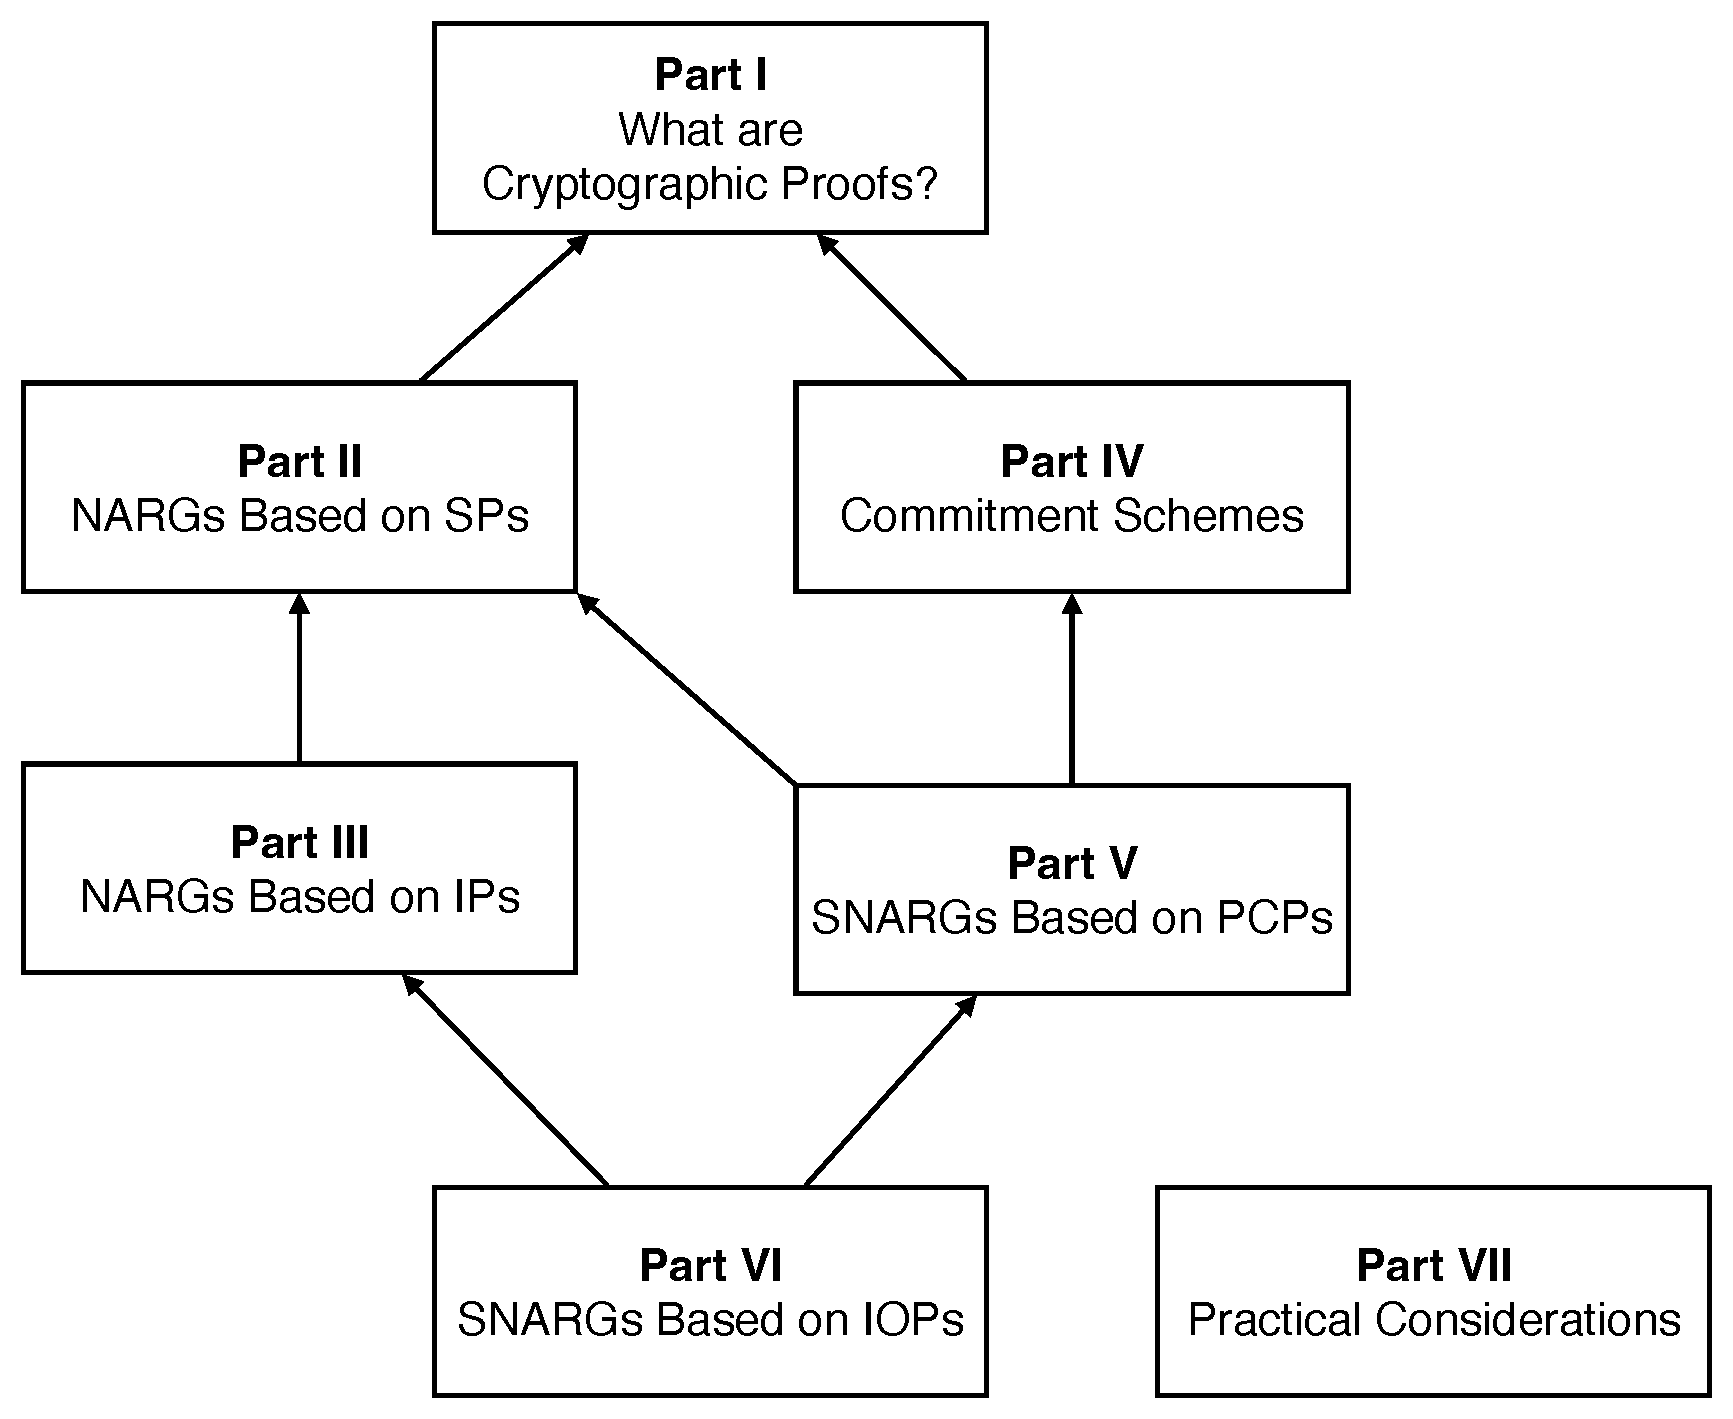
\includegraphics[width=0.7\textwidth]{\FigureFolder/part-dependency-diagram}
\caption[Parts of this book.]{Dependencies between the different parts of this book. (NARG stands for \emph{non-interactive argument}, and SNARG stands for \emph{succinct non-interactive argument}.)}
\label{figure:part-dependency-diagram}
\end{figure}

\begin{figure}[htp!]
\centering
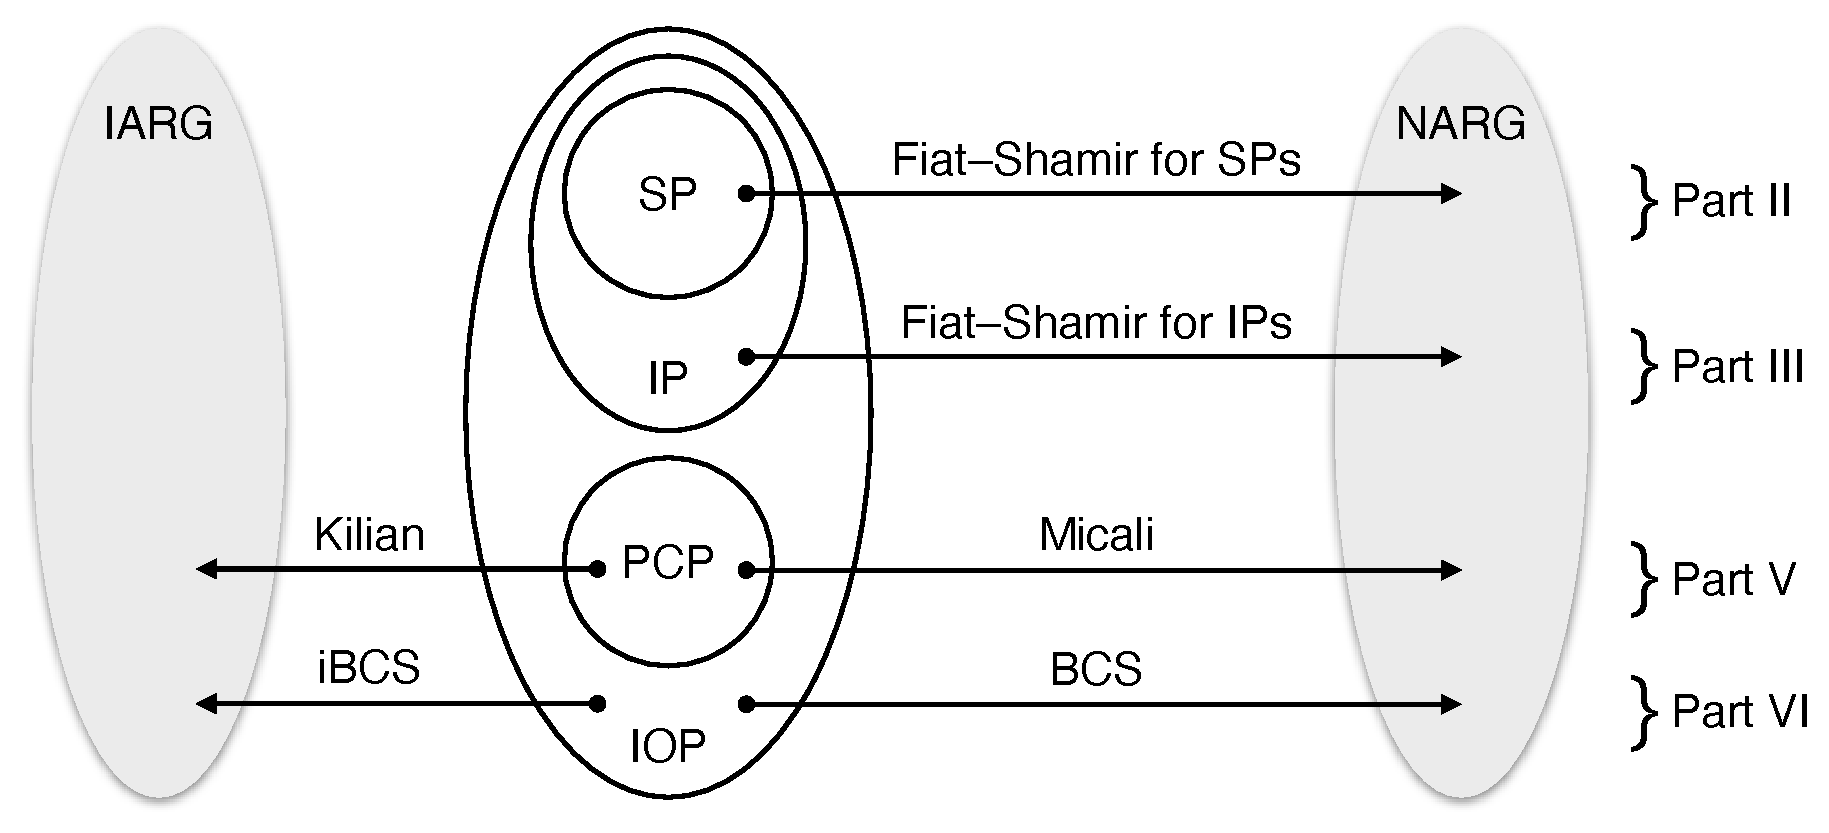
\includegraphics[width=0.8\textwidth]{\FigureFolder/transformations-summary-diagram}
\caption[Transformations in this book.]{All constructions of cryptographic proofs in this book are transformations applied to some type of probabilistic proof (SP, IP, PCP, or IOP). This diagram lists the transformations that we study, showing which ones construct an interactive argument (IARG) and which ones construct a non-interactive argument (NARG).}
\label{figure:transformations-summary-diagram}
\end{figure}

%%%%%%%%%%%%%%%%%%%%%%%%%%%%%%%%%%%%%%%%%%%%%%%%%%%%%%%%%%%%%%%%%%%%%%%%%%%%%%%
%%%%%%%%%%%%%%%%%%%%%%%%%%%%%%%%%%%%%%%%%%%%%%%%%%%%%%%%%%%%%%%%%%%%%%%%%%%%%%%
%%%%%%%%%%%%%%%%%%%%%%%%%%%%%%%%%%%%%%%%%%%%%%%%%%%%%%%%%%%%%%%%%%%%%%%%%%%%%%%
\section[nonumber=true]{How to use this book}

\parhead{Audience}
The book is aimed at people interested in understanding foundations and constructions of succinct arguments. The limited required background will make the material of this book accessible to different types of audiences.
\begin{itemize}
  \item \emph{Students.}
  An increasing number of undergraduate and graduate students wish to conduct research in cryptographic proofs, and SNARGs in particular. The material in this book enables students to gain familiarity with the main properties of argument systems in the simple ROM setting, and study how to write security reductions that transform a prover against an argument system into a prover against the underlying probabilistic proof.
  \item \emph{Practitioners.}
  Explicit and detailed constructions of several cryptographic proofs, presented with uniform notation and language, helps practitioners audit implementations. Moreover, the concrete security bounds helps practitioners set security parameters of implementations. This book includes several examples of how to make such choices.
\end{itemize}
Educators will also benefit from this book, as we outline below via examples of courses where material of this book will be useful.

\parhead{Usage}
The book can be used as a self-contained reference that a self-learner (e.g., a student or practitioner interested in the area) can follow chapter by chapter. For this it is useful to keep in mind the dependencies between parts of the book shown in \Cref{figure:part-dependency-diagram}.

Moreover, educators (e.g., a university professor) will find this book to be a useful didactic resource for certain courses. We give two examples.
\begin{itemize}
  \item \emph{Introductory cryptography.}
  An introductory cryptography course can benefit from discussions on the security definitions for argument systems in \Cref{part:what-are-crypto-proofs}, and from some of the simpler constructions of arguments. For example, the use of random oracles in \Cref{part:narg-from-sp} to remove interaction is a fundamental cryptographic paradigm known as the Fiat--Shamir transformation. Also, the succinct arguments in \Cref{part:snarg-from-pcp} are arguably among the simplest known, and have a strong pedagogical value (particularly so the Kilian transformation described there).
  \item \emph{Graduate course on cryptographic proofs.}
  A graduate course on cryptographic proofs may include a selection of material about probabilistic proofs and transformations to cryptographic proofs. This book provides a useful reference for some of the simplest such transformations, those based solely on ideal hash functions.
\end{itemize}



%%%%%%%%%%%%%%%%%%%%%%%%%%%%%%%%%%%%%%%%%%%%%%%%%%%%%%%%%%%%%%%%%%%%%%%%%%%%%%%
%%%%%%%%%%%%%%%%%%%%%%%%%%%%%%%%%%%%%%%%%%%%%%%%%%%%%%%%%%%%%%%%%%%%%%%%%%%%%%%
%%%%%%%%%%%%%%%%%%%%%%%%%%%%%%%%%%%%%%%%%%%%%%%%%%%%%%%%%%%%%%%%%%%%%%%%%%%%%%%
\section[nonumber=true]{Acknowledgements}

Work on this book was generously funded by:
\begin{itemize}[nolistsep]
  \item the \textbf{Ethereum Foundation};
  \item \textbf{Forte Labs};
  \item \textbf{Protocol Labs}; and
  \item \textbf{Provable}.
\end{itemize}
We are sincerely grateful that these entities agreed to support our vision of this book when it was conceived in the summer of 2021. Moreover, work on this book was done in part while working at \textbf{StarkWare Industries} and we are grateful for its support.

Our knowledge and enthusiasm about cryptographic proofs has greatly benefited from interactions with many wonderful colleagues and mentors over many years of academic research, as well as from forays into industry. We express our deepest gratitude to all of these colleagues.

Several people have generously agreed to review early drafts of this book, contributing valuable ideas, feedback, and corrections. We thank them in alphabetic order: Gal Arnon, Shany Ben-David, Zijing Di, Giacomo Fenzi, Ziyi Guan, Shai Keidar, Mathias Marty, Amit Sharabi, Yuxi Zheng.

Those who reported bugs and provided suggestions are acknowledged in the corresponding pull requests on this book's version history in the repository mentioned above.

Finally, we thank our families for tolerating our continuous work on this project for the past few years. Even if more prolonged and arduous than initially predicted, working on this project has been a joy, but would not have been possible without the generous support of our families.


%%%%%%%%%%%%%%%%%%%%%%%%%%%%%%%%%%%%%%%%%%%%%%%%%%%%%%%%%%%%%%%%%%%%%%%%%%%%%%%
\mainmatter
%%%%%%%%%%%%%%%%%%%%%%%%%%%%%%%%%%%%%%%%%%%%%%%%%%%%%%%%%%%%%%%%%%%%%%%%%%%%%%%


%%%%%%%%%%%%%%%%%%%%%%%%%%%%%%%%%%%%%%%%%%%%%%%%%%%%%%%%%%%%%%%%%%%%%%%%%%%%%%%
%%%%%%%%%%%%%%%%%%%%%%%%%%%%%%%%%%%%%%%%%%%%%%%%%%%%%%%%%%%%%%%%%%%%%%%%%%%%%%%
%%%%%%%%%%%%%%%%%%%%%%%%%%%%%%%%%%%%%%%%%%%%%%%%%%%%%%%%%%%%%%%%%%%%%%%%%%%%%%%
%%%%%%%%%%%%%%%%%%%%%%%%%%%%%%%%%%%%%%%%%%%%%%%%%%%%%%%%%%%%%%%%%%%%%%%%%%%%%%%
\addtocontents{toc}{\vspace{1.15\baselineskip}}
\chapter{Mathematical background}
\label{chapter:mathematical-background}

We introduce basic mathematical notation and facts that we use throughout this book.



%%%%%%%%%%%%%%%%%%%%%%%%%%%%%%%%%%%%%%%%%%%%%%%%%%%%%%%%%%%%%%%%%%%%%%%%%%%%%%%
%%%%%%%%%%%%%%%%%%%%%%%%%%%%%%%%%%%%%%%%%%%%%%%%%%%%%%%%%%%%%%%%%%%%%%%%%%%%%%%
%%%%%%%%%%%%%%%%%%%%%%%%%%%%%%%%%%%%%%%%%%%%%%%%%%%%%%%%%%%%%%%%%%%%%%%%%%%%%%%
\section{Notation}
\label{section:notation}

\parhead{Sets}
We denote by $\Cardinality{S}$ the cardinality of (i.e., number of elements in) a set $S$; if $S$ has an infinite number of elements then $\Cardinality{S} \DefineEqual \infty$. We denote by $\Reals$ the set of real numbers, by $\Naturals$ the set of positive integers $\{1,2,\dots\}$, and by $[n]$ the set of positive integers $\{1,2,\dots,n\}$. For $k \in \{0,1,\dots,n\}$, we denote by $\binom{[n]}{k}$ the set of all subsets of $[n]$ of cardinality $k$; the number of such subsets is $\binom{n}{k} \DefineEqual \frac{n!}{k! \cdot (n-k)!}$. We denote by $\{x_{1},\dots,x_{n}\}$ the set that contains the elements $x_{1},\dots,x_{n}$; its cardinality is the number of distinct elements among $x_{1},\dots,x_{n}$ (as duplicate elements are counted only once). Given a set $S$, we write $\{x_{i}\}_{i \in S}$ to denote the set that, for every $i \in S$, contains the element $x_{i}$; for example, $\{x_{i}\}_{i \in [n]}=\{x_{1},\dots,x_{n}\}$.

\parhead{Tuples}
A tuple is an ordered list of elements. We denote by $(x_{i})_{i \in [n]}$ the tuple $(x_{1},\ldots,x_{n})$; more generally, $(x_{i})_{i \in S}$ denotes a tuple whose entries are indexed by elements of a given set $S$ according to a canonical order. Duplicate elements in a tuple appear multiple times, at the appropriate locations. Tuples of tuples are obtained by nesting parentheses; for example, $((x_{i},y_{i},z_{i}))_{i \in [n]}$ is the tuple of tuples $((x_{1},y_{1},z_{1}),\dots,(x_{n},y_{n},z_{n}))$. If $x$ is a tuple whose entries are indexed by a set $S$ then, for every $i \in S$, $x[i]$ is the $i$-th entry of $x$; more generally, for a subset $T \subseteq S$, $x[T]$ denotes the tuple obtained by considering the entries of $x$ whose indices are in $T$. For example, if $x = (x_{i})_{i \in \{1,4,7\}}$ then $x[7]=x_{7}$ and $x[\{1,7\}]=(x_{i})_{i \in \{1,7\}}$.

\parhead{Strings}
Let $\ProtoAlphabet$ be a finite alphabet (i.e., a finite set). A string over $\ProtoAlphabet$ is a function $x \colon D \to \ProtoAlphabet$ over some ordered set $D$ that takes values in $\ProtoAlphabet$; in particular, $x$ is a tuple $(x_{i})_{i \in D}$ where every entry $x_{i}$ is an element of the alphabet $\ProtoAlphabet$. Typically $D=[n]$ for some $n \in \Naturals$, in which case we may write the string by listing the symbols in a sequence; for example, $001$ represents the string $x \colon [3] \to \Bits$ where $x_{1}=0$, $x_{2}=0$, and $x_{3}=1$. We use $\concat$ to denote string concatenation; for example $00 \concat 1$ is the string $001$.

For every $n \in \Naturals$, we denote by $\ProtoAlphabet^{n}$ the set of all strings over $\ProtoAlphabet$ of length $n$:
\begin{equation*}
\ProtoAlphabet^{n}
\DefineEqual
\left\{
x \colon [n] \to \ProtoAlphabet
\right\}
=
\left\{
(x_{i})_{i \in [n]} : \forall\, i \in [n], \; x_{i} \in \ProtoAlphabet
\right\}
\enspace.
\end{equation*}
We denote by $\ProtoAlphabet^{*} \DefineEqual \cup_{n \in \Naturals} \ProtoAlphabet^{n}$ the set of all finite-length strings over $\ProtoAlphabet$.

Given an ordered set $D$, we denote by $\ProtoAlphabet^{D}$ the set of strings over $\ProtoAlphabet$ of length $\Cardinality{D}$ whose entries are indexed by elements of $D$:
\begin{equation*}
\ProtoAlphabet^{D}
\DefineEqual
\left\{
x \colon D \to \ProtoAlphabet
\right\}
=
\left\{
(x_{i})_{i \in D} : \forall\, i \in D, \; x_{i} \in \ProtoAlphabet
\right\}
\enspace.
\end{equation*}
For example, if $\ProtoAlphabet = \Bits$ and $D = \{1,8,9\}$, then a string $x$ in $ \ProtoAlphabet^{D}=\Bits^{\{1,8,9\}}$ may have the following values: $x[1] = 0$, $x[8] = 1$, and $x[9]=0$.

\parhead{Bit lengths}
A binary string is a string over the alphabet $\ProtoAlphabet=\Bits$. We denote by $\BitSize{x}$ the length of a binary string $x \in \Bits^{*}$; for example $\BitSize{001}=3$. If $x$ is not a binary string then $\BitSize{x}$ denotes the length of a suitable representation of $x$ as a binary string. For example, if $x$ is a string in $\ProtoAlphabet^{n}$ then $\BitSize{x} = n \cdot \ceil{\log_{2} \Cardinality{\ProtoAlphabet}}$ by representing each of the $n$ symbols in $x$ as a $\ceil{\log_{2} \Cardinality{\ProtoAlphabet}}$-bit string (representing the appropriate symbol in $\ProtoAlphabet$ as a binary string). If $x$ is a string in $\ProtoAlphabet^{D}$ then $\BitSize{x} = n \cdot (\ceil{\log_{2} \Cardinality{D}} + \ceil{\log_{2} \Cardinality{\ProtoAlphabet}})$ by representing $x$ as a list of pairs: if $x=(x_{i})_{i \in D}$ then $x$ is encoded as a list of $n$ pairs, each pair consisting of a $\ceil{\log_{2} \Cardinality{D}}$-bit string encoding an index $i$ and a $\ceil{\log_{2} \Cardinality{\ProtoAlphabet}}$-bit string encoding the symbol $x_{i}$.

\parhead{Sampling}
We denote by $a \gets D$ the process of sampling $a$ according to the distribution $D$. Similarly, given a finite set $S$, we denote by $a \gets S$ the process of sampling $a$ according to the uniform distribution over $S$.

\parhead{Asymptotics}
We use standard asymptotic notation. For example, given two functions $f,g \colon \Naturals \to \Reals$, we write $f(n) = O(g(n))$ and $f(n) = \Omega(g(n))$ to respectively denote the fact that there exists a constant $c>0$ such that, for all large enough $n$, it holds that $f(n) \leq c \cdot g(n)$ and $f(n) \geq c \cdot g(n)$. Moreover, we write $f(n) = o(g(n))$ and $f(n) = \omega(g(n))$ to respectively denote the fact that for every constant $c>0$, for all large enough $n$, it holds that $f(n) \leq c \cdot g(n)$ and $f(n) \geq c \cdot g(n)$. We additionally use notation to refer to some unspecified polynomially-bounded function: $\poly(n)$ denotes $n^{O(1)}$ and, more generally, $\poly(n_{1},n_{2},\dots)$ denotes $(n_{1}+n_{2}+\cdots)^{O(1)}$.

\parhead{Languages and relations}
A relation $\Relation$ is a set consisting of instance-witness pairs $(\Instance,\Witness)$. The corresponding language $\GetLanguage{\Relation}$ is the set of instances $\Instance$ for which there exists a witness $\Witness$ such that $(\Instance,\Witness)$ is in the relation $\Relation$. We write $\SomeSize{\Instance}$ to denote the size of an instance; this could be the number of bits to describe $\Instance$ (namely, $\BitSize{\Instance}$) or some other measure suitable for instances of the relation $\Relation$.

\parhead{Algorithms}
We informally refer to algorithms as procedures running on an appropriate computation model. If we are not interested in the time or space complexity of an algorithm (such as when we consider unbounded adversaries), then the underlying computation model does not matter. (It does not matter whether it is a single-tape Turing machine, multi-tape Turing machine, register machine, or other.) If we discuss the time or space complexity of an algorithm then we assume that the algorithm is running on a register machine that resembles a modern computer (a finite set of instructions with read/write random-access to memory with appropriate word length). We consider both deterministic algorithms and probabilistic algorithms (which additionally have access to a string of random bits of a certain length).

An algorithm runs in polynomial time if its running time is upper bounded by a polynomial in the size of its input. (If the algorithm has multiple inputs, then we consider the sum of their sizes.)

\parhead{Interactive algorithms}
An algorithm $A$ is \emph{interactive} if it maintains state across multiple input-to-output invocations. The outputs of $A$ given sequence of inputs $a_{1},a_{2},a_{3},\dots$ are as follows:
\begin{equation*}
b_{1} \gets A(a_{1}),\;
b_{2} \gets A(a_{2}),\;
b_{3} \gets A(a_{3}),\;
\dots
\enspace.
\end{equation*}
Sometimes, it is helpful to make explicit the state passed from one execution to the next, in which case we view the algorithm $A$ as stateless:
\begin{equation*}
(b_{1},\AuxiliaryState_{1}) \gets A(a_{1}),\;
(b_{2},\AuxiliaryState_{2}) \gets A(\AuxiliaryState_{1},a_{2}),\;
(b_{3},\AuxiliaryState_{3}) \gets A(\AuxiliaryState_{2},a_{3}),\;
\dots
\enspace.
\end{equation*}

\parhead{Black boxes}
Sometimes we describe algorithms that receive other algorithms as input and rely only on their input-output functionality (by running them on certain inputs and obtaining corresponding outputs), rather than also using their description. We emphasize when this is the case by saying that they are used as \emph{black boxes}.

Let $A$ and $B$ be algorithms. We say that \emph{$A$ uses $B$ as a black-box}, denoted $A(\BlackBox{B})$, if $A$ invokes $B$ some number of times (on inputs of its choice) and otherwise does not \DoQuote{look} at $B$'s description. More precisely, for every two algorithms $B_{1}$ and $B_{2}$ that represent the same function, $A(\BlackBox{B_{1}}) = A(\BlackBox{B_{2}})$.

If $B$ is an interactive algorithm, then we define $\BlackBox{B}$ to be the black box for the \emph{stateless} representation of $B$, namely, the black box for the function that given an internal state of $B$ and an input for $B$ returns the corresponding output of $B$ and resulting internal state. In particular, $A(\BlackBox{B})$ can interact with $B$ on a sequence of inputs $a_{1},a_{2},a_{3},\dots$ as follows:
\begin{equation*}
(b_{1},\AuxiliaryState_{1}) \gets \BlackBox{B}(a_{1}),\;
(b_{2},\AuxiliaryState_{2}) \gets \BlackBox{B}(\AuxiliaryState_{1},a_{2}),\;
(b_{3},\AuxiliaryState_{3}) \gets \BlackBox{B}(\AuxiliaryState_{2},a_{3}),\;
\dots
\enspace.
\end{equation*}

There is a subtle technicality in the above sequence of black-box invocations. The (arbitrary) internal states $(\AuxiliaryState_{i})_{i}$ received by $A$ from (the stateless representation of) $B$ may contain \emph{non-black-box} information about the algorithm $B$ (e.g., the code of $B$); moreover, the internal states $(\AuxiliaryState_{i})_{i}$ may be large (e.g., of exponential size if $B$ is inefficient), impacting the efficiency of $A$. Yet $A$ is only interested in the input-output behavior of $B$, and we wish to ensure that a black-box invocation of $B$ does not burden $A$ with $B$'s inefficiencies. However, $A$ needs $B$'s internal states in order to facilitate multiple invocations of $B$ from the same execution point on different inputs.

This technicality is resolved by regarding the internal states $(\AuxiliaryState_{i})_{i}$ as merely \emph{handles} to the actual (possibly large) internal states. These handles allow the algorithm $A$ to invoke $B$ as needed by specifying the handle of an internal state rather than the internal state itself (which is not exposed to $A$). If $A$ performs at most $t$ invocations, then at most $t$ handles are needed, so each handle can be expressed as a $\ceil{\log t}$-bit string. For simplicity, we slightly abuse notation and use the same notation $(b_{i},\AuxiliaryState_{i}) \gets \BlackBox{B}(\AuxiliaryState_{i-1},a_{i})$ as above.

\parhead{Malicious parties}
We often (though not always) put a tilde over symbols that refer to malicious parties: if $P$ is the symbol that we would use for an honest party, then $\Malicious{P}$ denotes a malicious party. (A malicious party is one that does not necessarily follow the prescribed instructions of a protocol.)



%%%%%%%%%%%%%%%%%%%%%%%%%%%%%%%%%%%%%%%%%%%%%%%%%%%%%%%%%%%%%%%%%%%%%%%%%%%%%%%
%%%%%%%%%%%%%%%%%%%%%%%%%%%%%%%%%%%%%%%%%%%%%%%%%%%%%%%%%%%%%%%%%%%%%%%%%%%%%%%
%%%%%%%%%%%%%%%%%%%%%%%%%%%%%%%%%%%%%%%%%%%%%%%%%%%%%%%%%%%%%%%%%%%%%%%%%%%%%%%
\section{Probability}
\label{section:probability}

\parhead{Events}
We denote by $\Pr[\Event]$ the probability of an event $\Event$, which is a real number in $[0,1]$. For example, if $b$ is a random bit then $\Pr[b = 0]=\frac{1}{2}$. We use logical operators on events: $\Negate{\Event}$ is the negation of $\Event$; $\Event_{1} \land \Event_{2}$ is the event where $\Event_{1}$ and $\Event_{2}$ hold; $\Event_{1} \lor \Event_{2}$ is the event where $\Event_{1}$ or $\Event_{2}$ holds; and so on. For example, $\Pr[\Event \land \Negate{\Event}]=0$ and $\Pr[\Event] + \Pr[\Negate{\Event}] = 1$.

Two events $\Event_{1}$ and $\Event_{2}$ are independent if (and only if) $\Pr[\Event_{1} \land \Event_{2}] = \Pr[\Event_{1}] \cdot \Pr[\Event_{2}]$. In other words, the probability that both events hold simultaneously equals the product of the two probabilities where each event holds individually.

The probability of the event $\Event_{1}$ conditioned on the event $\Event_{2}$ is $\Pr\left[\Event_{1} \ConditionedOn \Event_{2}\right] \DefineEqual \frac{\Pr[\Event_{1} \land \Event_{2}]}{\Pr[\Event_{2}]}$. This probability is defined only when $\Pr[\Event_{2}] > 0$. If $\Event_{1}$ and $\Event_{2}$ are independent then $\Pr\left[\Event_{1} \ConditionedOn \Event_{2}\right] = \Pr[\Event_{1}]$. (Conversely, if $\Pr[\Event_{2}] > 0$ and $\Pr\left[\Event_{1} \ConditionedOn \Event_{2}\right] = \Pr[\Event_{1}]$ then $\Event_{1}$ and $\Event_{2}$ are independent.)

The law of total probability states that the probability of an event can be split across a collection of events that partition the probability space.

\begin{lemma}[law of total probability]
\label{lemma:law-of-total-probability}
Let $\Event_{1}$ be an event.
\begin{itemize}

  \item For every $\Event_{2}$,
\begin{equation*}
\Pr[\Event_{1}]
=
\Pr[\Event_{1} \land \Event_{2}]
+
\Pr[\Event_{1} \land \Negate{\Event_{2}}]
\enspace.
\end{equation*}

  \item More generally, for every collection of events $\Event_{2,1},\dots,\Event_{2,n}$ that partition the probability space (such that $\Pr[\idxlor{i \in [n]} \Event_{2,i}]=1$ and $\Pr[\Event_{2,i} \land \Event_{2,j}]=0$ for every distinct $i,j \in [n]$),
\begin{equation*}
\Pr[\Event_{1}]
=
\sum_{i \in [n]} \Pr[\Event_{1} \land \Event_{2,i}]
\enspace.
\end{equation*}
\end{itemize}
If all the relevant conditional probabilities are well-defined, the equalities above can be rewritten as
\begin{align*}
\Pr[\Event_{1}]
&=
\Pr\left[\Event_{1} \ConditionedOn \Event_{2}\right]
  \cdot \Pr[\Event_{2}]
+
\Pr\left[\Event_{1} \ConditionedOn \Negate{\Event_{2}}\right]
  \cdot \Pr[\Negate{\Event_{2}}]
\enspace\text{and}
\\
\Pr[\Event_{1}]
&=
\sum_{i \in [n]}
\Pr\left[\Event_{1} \ConditionedOn \Event_{2,i}\right]
  \cdot \Pr[\Event_{2,i}]
\enspace.
\end{align*}
\end{lemma}

The addition rule provides a way to express the probability of the union of two events:
\begin{equation*}
\Pr[\Event_{1} \lor \Event_{2}]
=
\Pr[\Event_{1}]+\Pr[\Event_{2}]-\Pr[\Event_{1} \land \Event_{2}]
\enspace.
\end{equation*}
Intuitively, $\Pr[\Event_{1}]+\Pr[\Event_{2}]$ double counts where $\Event_{1}$ and $\Event_{2}$ intersect, and so subtracting $\Pr[\Event_{1} \land \Event_{2}]$ corrects for this. In particular, we learn that $\Pr[\Event_{1} \lor \Event_{2}] \leq \Pr[\Event_{1}]+\Pr[\Event_{2}]$.

More generally, if there are more than two events, there can be intersections among any number of the events, leading to more complicated combinatorics of corrections. For example, for three events (see \Cref{figure:inclusive-exclusive-diagram} for an illustration):
\begin{align*}
\Pr[\Event_{1} \lor \Event_{2} \lor \Event_{3}]
&=
\Pr[\Event_{1}]+\Pr[\Event_{2}]+\Pr[\Event_{3}]
\\&-\Pr[\Event_{1} \land \Event_{2}]-\Pr[\Event_{2} \land \Event_{3}]-\Pr[\Event_{3} \land \Event_{1}]
\\&+\Pr[\Event_{1} \land \Event_{2} \land \Event_{3}]
\enspace.
\end{align*}
Since $\Pr[\Event_{1} \land \Event_{2} \land \Event_{3}] \geq 0$, this equality implies a simple lower bound:
\begin{align*}
\Pr[\Event_{1} \lor \Event_{2} \lor \Event_{3}]
\geq
\sum_{i \in [3]} \Pr[\Event_{i}] -
\sum_{\substack{i,j \in [3] \\ \text{with } i \neq j}} \Pr[\Event_{i} \land \Event_{j}]
\enspace.
\end{align*}
Moreover, since $\Pr[\Event_{1} \land \Event_{2} \land \Event_{3}] \leq \Pr[\Event_{1} \land \Event_{2}]$, this equality also implies a simple upper bound:
\begin{align*}
\Pr[\Event_{1} \lor \Event_{2} \lor \Event_{3}]
\leq
\sum_{i \in [3]} \Pr[\Event_{i}]
\enspace.
\end{align*}

\begin{figure}[htp!]
\centering
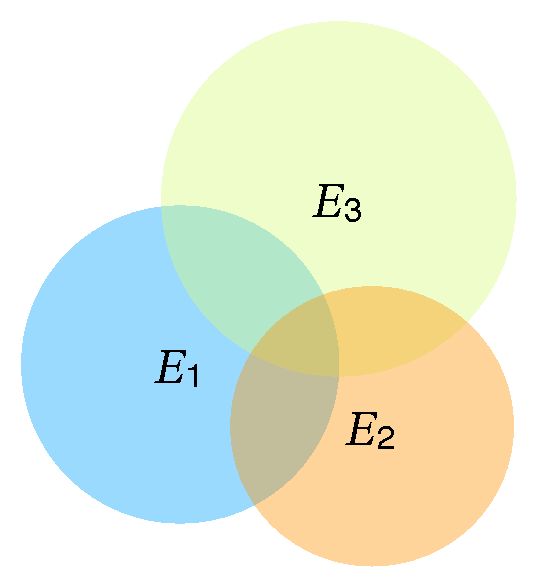
\includegraphics[width=0.3\textwidth]{\FigureFolder/inclusive-exclusive-diagram}
\caption[Pairwise and three-wise interaction of $3$ events.]{Diagram of the pairwise and three-wise intersections of events $\Event_{1},\Event_{2},\Event_{3}$.}
\label{figure:inclusive-exclusive-diagram}
\end{figure}

The general case is called the \emph{inclusion-exclusion principle}, which provides a way to express the probability of the union of $n$ events $\Event_{1},\ldots,\Event_{n}$ as a (signed) sum of the probabilities of all their intersections.

\begin{lemma}[inclusion–exclusion principle]
\label{lemma-inclusion-exclusion}
For every $n$ events $\Event_{1},\ldots,\Event_{n}$ it holds that
\begin{align*}
  \Pr\left[\idxlor{i \in [n]} \Event_{i} \right] =
  \sum_{k \in [n]}
    \left(
    (-1)^{k+1}
    \cdot
    \sum_{\substack{I \subseteq [n] \\ \text{with } \Cardinality{I}=k}} \Pr\left[\idxland{i \in I} \Event_{i} \right]
    \right)
\enspace.
\end{align*}
\end{lemma}

The equality in the above lemma can be inconvenient to use because it involves many terms. The statement below about the probability of $\idxlor{i \in [n]} \Event_{i}$ is simpler to use: it provides a lower bound and an upper bound in terms of the individual probabilities of the single events $\Event_{i}$ and of their pairwise intersections $\Event_{i} \land \Event_{j}$.

\begin{lemma}[simple inclusion–exclusion principle]
\label{lemma:inclusion-exclusion-2}
For every $n$ events $\Event_{1},\ldots,\Event_{n}$,
\begin{align*}
\sum_{i \in [n]} \Pr[\Event_{i}] -
\sum_{\substack{i,j \in [n] \\ \text{with } i \neq j}} \Pr[\Event_{i} \land \Event_{j}]
\leq
\Pr
\left[\idxlor{i \in [n]} \Event_{i} \right]
\leq
\sum_{i \in [n]} \Pr[\Event_{i}]
\enspace.
\end{align*}
\end{lemma}

\begin{proof}
We give a proof by induction on the number of events $n$.

\emph{Base case: $n \in \{1,2,3\}$.}
The case for $n=1$ holds because all expressions in the lemma are $\Pr[\Event_{1}]$. Separately, in the discussion before the lemma we prove the cases where $n=2$ and $n=3$.

\emph{Inductive case: $n > 1$.}
We prove the lemma for $n$ assuming that the lemma holds for every $n' \in [n-1]$. Define the event $\Event^{*} \DefineEqual \idxlor{i \in [n-1]} \Event_{i}$.
By the induction hypothesis for $n' = n-1$,
\begin{align}
\label{equation:inclusion-exclusion-2-eq1}
\sum_{i \in [n-1]} \Pr[\Event_{i}] -
\sum_{\substack{i,j \in [n-1] \\ \text{with } i \neq j}} \Pr[\Event_{i} \land \Event_{j}]
\leq
\Pr
\left[\Event^{*} \right]
\leq
\sum_{i \in [n-1]} \Pr[\Event_{i}]
\enspace.
\end{align}
First we prove the upper bound. By the induction hypothesis for $n'=2$ (on the events $\Event^{*}$ and $\Event_{n}$), and by \Cref{equation:inclusion-exclusion-2-eq1}, we have that
\begin{align*}
\Pr\left[\Event^{*} \lor \Event_{n} \right]
\leq \Pr[\Event^{*}] + \Pr[\Event_{n}]
\leq \sum_{i \in [n-1]} \Pr[\Event_{i}] + \Pr[\Event_{n}]
= \sum_{i \in [n]} \Pr[\Event_{i}]
\enspace.
\end{align*}
Next we prove the lower bound. Applying the (now proved) upper bound to the events $\{\Event_{i} \land \Event_{n}\}_{i \in [n]}$, we obtain
\begin{align}
\label{equation:inclusion-exclusion-2-eq2}
\Pr[\idxlor{i \in [n]} (\Event_{i} \land \Event_{n})]
\leq \sum_{i \in [n]}\Pr[\Event_{i} \land \Event_{n}]
\enspace.
\end{align}
By the induction hypothesis for $n'=2$ (on the events $\Event^{*}$ and $\Event_{n}$), and by \Cref{equation:inclusion-exclusion-2-eq1,equation:inclusion-exclusion-2-eq2}, we have that
\begin{align*}
& \Pr\left[\Event^{*} \lor \Event_{n} \right]
\\ & \geq
\Pr[\Event^{*}] + \Pr[\Event_{n}] - \Pr[\Event^{*} \land \Event_{n}]
\\ & \geq
\left(\sum_{i \in [n-1]} \Pr[\Event_{i}] - \sum_{\substack{i,j \in [n-1] \\ \text{with } i \neq j}} \Pr[\Event_{i} \land \Event_{j}] \right) + \Pr[\Event_{n}] - \Pr[\Event^{*} \land \Event_{n}]
\\ & =
\sum_{i \in [n]} \Pr[\Event_{i}] - \sum_{\substack{i,j \in [n-1] \\ \text{with } i \neq j}} \Pr[\Event_{i} \land \Event_{j}] - \Pr[\idxlor{i \in [n]} (\Event_{i} \land \Event_{n})]
\\ & \geq
\sum_{i \in [n]} \Pr[\Event_{i}] -
\sum_{\substack{i,j \in [n] \\ \text{with } i \neq j}} \Pr[\Event_{i} \land \Event_{j}]
\enspace.
\end{align*}
\end{proof}

We describe events via expressions that involve random variables. In this book random variables take values that are binary strings or real values. In the latter case, a binary random variable is one that takes only values that are zero or one.

\parhead{Random variables}
If $\RandomVariableX$ is a random variable that takes values in a finite set $\RandomVariableSupport \subseteq \Reals$ then we can define its \emph{expectation} as follows:
\begin{equation*}
\Expectation[\RandomVariableX]
\DefineEqual
\sum_{x \in \RandomVariableSupport}
x \cdot \Pr[\RandomVariableX=x]
\enspace.
\end{equation*}
Two random variables $\RandomVariableX$ and $\RandomVariableY$ are independent if (and only if) for every $x$ and $y$ it holds that $\Pr[\RandomVariableX=x \land \RandomVariableY=y] = \Pr[\RandomVariableX=x] \cdot \Pr[\RandomVariableY=y]$. More generally, the random variables $\RandomVariableX_{1},\dots,\RandomVariableX_{n}$ are independent if (and only if) for every $x_{1},\dots,x_{n}$ it holds that $\Pr[\idxland{i \in [n]}\RandomVariableX_{i}=x_{i}] = \prod_{i \in [n]} \Pr[\RandomVariableX_{i}=x_{i}]$.

The law of large numbers states that, given an infinite sequence of random variables $\{\RandomVariableX_{i}\}_{i \in \Naturals}$ that are independently and identically distributed, $\Expectation[\RandomVariableX]$ is the limit of $\frac{1}{n} \sum_{i \in [n]} \RandomVariableX_{i}$ as $n$ tends to infinity. The distance of $\frac{1}{n} \sum_{i \in [n]} \RandomVariableX_{i}$ from $\Expectation[\RandomVariableX]$ as a function of $n$ is captured by \emph{concentration bounds}. One example, is the following (additive) \emph{Chernoff bound}.



\begin{lemma}[Chernoff bound]
\label{lemma:chernoff-bound}
Let $\RandomVariableX_{1},\ldots,\RandomVariableX_{n}$ be independent binary random variables such that $\Pr[\RandomVariableX_{i}=1] = p_{i}$ for every $i \in [n]$. Let $\RandomVariableX \DefineEqual \sum_{i \in [n]} \RandomVariableX_{i}$ and $\mu \DefineEqual \Expectation[\RandomVariableX] = \sum_{i \in [n]}p_{i}$. For every $\delta \in (0,1)$,
\begin{align*}
\Pr[\AbsValue{\RandomVariableX - \mu} \geq \delta \cdot \mu]
\leq 2 \cdot e^{-\frac{\mu \delta^2}{3}}
\enspace.
\end{align*}
\end{lemma}

\parhead{Statistical distance}
We measure the statistical distance between two random variables in terms of their total variation distance, as in the definition below.

\begin{definition}
\label{definition:statistical-distance}
The \defemph{statistical distance} between two random variables $\RandomVariableX$ and $\RandomVariableY$ taking values in a finite set $\RandomVariableSupport$ is defined as
\begin{equation}
\label{definition:statistical-distance-def1}
\StatisticalDistance{\RandomVariableX}{\RandomVariableY}
\DefineEqual
\frac{1}{2} \sum_{a \in \RandomVariableSupport} \AbsValue{\Pr[\RandomVariableX=a]-\Pr[\RandomVariableY=a]}
\enspace.
\end{equation}
Equivalently, the statistical distance can also be defined as
\begin{equation}
\label{definition:statistical-distance-def2}
\StatisticalDistance{\RandomVariableX}{\RandomVariableY}
\DefineEqual
\max_{\RandomVariableSupport' \subseteq \RandomVariableSupport} \AbsValue{\Pr[\RandomVariableX \in \RandomVariableSupport']-\Pr[\RandomVariableY \in \RandomVariableSupport']}
\enspace.
\end{equation}
\end{definition}



We show that the two definitions given above (\Cref{definition:statistical-distance-def1,definition:statistical-distance-def2}) are equivalent.

\begin{claim}
The definition using \Cref{definition:statistical-distance-def1} is equivalent to the definition using \Cref{definition:statistical-distance-def2}.
\end{claim}

\begin{proof}
Define the subset $\RandomVariableSupport_{0} \subseteq \RandomVariableSupport$ as
\begin{equation*}
\RandomVariableSupport_{0}
\DefineEqual
\{ a \in \RandomVariableSupport : \Pr[\RandomVariableX=a] \geq \Pr[\RandomVariableY=a] \}
\enspace.
\end{equation*}
Additionally, let $\RandomVariableSupport_{1}$ be the complement set: $\RandomVariableSupport_{1} \DefineEqual \RandomVariableSupport \setminus \RandomVariableSupport_{0}$.

Observe that $\Pr[\RandomVariableX \in \RandomVariableSupport_{0}] + \Pr[\RandomVariableX \in \RandomVariableSupport_{1}] = 1$ and $\Pr[\RandomVariableY \in \RandomVariableSupport_{0}] + \Pr[\RandomVariableY \in \RandomVariableSupport_{1}] = 1$. Hence
\begin{equation}
\label{equation:statistical-distance-eq1}
\Pr[\RandomVariableX \in \RandomVariableSupport_{0}] - \Pr[\RandomVariableY \in \RandomVariableSupport_{0}]
=
\Pr[\RandomVariableY \in \RandomVariableSupport_{1}] - \Pr[\RandomVariableX \in \RandomVariableSupport_{1}]
\enspace.
\end{equation}

One can argue that $\RandomVariableSupport_{0}$ or $\RandomVariableSupport_{1}$ maximizes the expression $\max_{\RandomVariableSupport' \subseteq \RandomVariableSupport} \AbsValue{\Pr[\RandomVariableX \in \RandomVariableSupport']-\Pr[\RandomVariableY \in \RandomVariableSupport']}$. Then, using \Cref{equation:statistical-distance-eq1}, we get that
\begin{align*}
\Pr[\RandomVariableY \in \RandomVariableSupport_{1}] - \Pr[\RandomVariableX \in \RandomVariableSupport_{1}]
=
\max_{\RandomVariableSupport' \subseteq \RandomVariableSupport} \AbsValue{\Pr[\RandomVariableX \in \RandomVariableSupport']-\Pr[\RandomVariableY \in \RandomVariableSupport']}
=
\Pr[\RandomVariableX \in \RandomVariableSupport_{0}]-\Pr[\RandomVariableY \in \RandomVariableSupport_{0}]
\enspace.
\end{align*}

Finally, we write
\begin{align*}
\StatisticalDistance{\RandomVariableX}{\RandomVariableY}
& \DefineEqual
\frac{1}{2} \sum_{a \in \RandomVariableSupport} \AbsValue{\Pr[\RandomVariableX=a]-\Pr[\RandomVariableY=a]}
\\ & =
\frac{1}{2} \left( \sum_{a \in \RandomVariableSupport_{0}} \left( \Pr[\RandomVariableX=a]-\Pr[\RandomVariableY=a] \right) +
\sum_{a \in \RandomVariableSupport_{1}} \left( \Pr[\RandomVariableY=a]-\Pr[\RandomVariableX=a] \right) \right)
\\ & =
\frac{1}{2} \left( \Pr[\RandomVariableX \in \RandomVariableSupport_{0}]-\Pr[\RandomVariableY \in \RandomVariableSupport_{0}] +
\Pr[\RandomVariableY \in \RandomVariableSupport_{1}] - \Pr[\RandomVariableX \in \RandomVariableSupport_{1}] \right)
\\ & =
\frac{1}{2} \left( \Pr[\RandomVariableX \in \RandomVariableSupport_{0}]-\Pr[\RandomVariableY \in \RandomVariableSupport_{0}] +
(1-\Pr[\RandomVariableY \in \RandomVariableSupport_{0}]) - (1-\Pr[\RandomVariableX \in \RandomVariableSupport_{0}]) \right)
\\ & =
\Pr[\RandomVariableX \in \RandomVariableSupport_{0}] - \Pr[\RandomVariableY \in \RandomVariableSupport_{0}]
\\ & =
\max_{\RandomVariableSupport' \subseteq \RandomVariableSupport} \AbsValue{\Pr[\RandomVariableX \in \RandomVariableSupport']-\Pr[\RandomVariableY \in \RandomVariableSupport']}
\enspace.
\end{align*}
\end{proof}

The following claim states basic properties about statistical distance that we use.

\begin{claim}
\label{claim:triangle-inequality-statistical-distance}
The statistical distance function satisfies the following properties.
\begin{enumerate}[noitemsep]
  \item For every random variable $\RandomVariableX$, $\StatisticalDistance{\RandomVariableX}{\RandomVariableX} = 0$.
  \item For every random variables $\RandomVariableX,\RandomVariableY$, $0 \leq \StatisticalDistance{\RandomVariableX}{\RandomVariableY} \leq 1$.
  \item For every random variables $\RandomVariableX,\RandomVariableY,\RandomVariableZ$, $\StatisticalDistance{\RandomVariableX}{\RandomVariableZ} \leq \StatisticalDistance{\RandomVariableX}{\RandomVariableY} + \StatisticalDistance{\RandomVariableY}{\RandomVariableZ}$.
\end{enumerate}
\end{claim}

\begin{proof}
The first two properties follow directly from the definition. We prove the third property as follows:
\begin{align*}
\StatisticalDistance{\RandomVariableX}{\RandomVariableZ}
& =
\frac{1}{2} \sum_{a} \AbsValue{\Pr[\RandomVariableX=a]-\Pr[\RandomVariableZ=a]}
\\ & =
\frac{1}{2} \sum_{a} \AbsValue{\big(\Pr[\RandomVariableX=a]-\Pr[\RandomVariableY=a]\big) + \big(\Pr[\RandomVariableY = a] - \Pr[\RandomVariableZ = a]\big)}
\\ & \leq
\frac{1}{2} \sum_{a} \AbsValue{\Pr[\RandomVariableX=a]-\Pr[\RandomVariableY=a]} +
\frac{1}{2} \sum_{a} \AbsValue{(\Pr[\RandomVariableY = a] - \Pr[\RandomVariableZ = a])}
\\ & =
\StatisticalDistance{\RandomVariableX}{\RandomVariableY} + \StatisticalDistance{\RandomVariableY}{\RandomVariableZ}
\enspace.
\end{align*}
\end{proof}

The following claim states that manipulating two random variables $\RandomVariableX$ and $\RandomVariableY$ by applying the same function $f$ does not increase their statistical distance.

\begin{claim}
\label{claim:function-and-statistical-distance}
For every two random variables $\RandomVariableX,\RandomVariableY$ over a domain $\RandomVariableSupport$ and function $f$ defined over $\RandomVariableSupport$,
\begin{equation*}
\StatisticalDistance{f(\RandomVariableX)}{f(\RandomVariableY)}
\leq
\StatisticalDistance{\RandomVariableX}{\RandomVariableY}
\enspace.
\end{equation*}
\end{claim}

\begin{proof}
\begin{align*}
\StatisticalDistance{f(\RandomVariableX)}{f(\RandomVariableY)}
& =
\frac{1}{2} \sum_{b \in f(\RandomVariableSupport)} \AbsValue{\Pr[f(\RandomVariableX)=b]-\Pr[f(\RandomVariableY)=b]}
\\ & =
\frac{1}{2}
\sum_{b \in f(\RandomVariableSupport)}
\AbsValue{\sum_{a \in f^{(-1)}(b)}
\Pr[\RandomVariableX=a]-\Pr[\RandomVariableY=a]}
\\ & \leq
\frac{1}{2}
\sum_{b \in f(\RandomVariableSupport)}
\sum_{a \in f^{(-1)}(b)}
\AbsValue{\Pr[\RandomVariableX=a]-\Pr[\RandomVariableY=a]}
\\ & \leq
\frac{1}{2}
\sum_{a \in \RandomVariableSupport}
\AbsValue{\Pr[\RandomVariableX=a]-\Pr[\RandomVariableY=a]}
\\ & \leq
\StatisticalDistance{\RandomVariableX}{\RandomVariableY}
\enspace.
\end{align*}
\end{proof}

Suppose that we have a random variable $\RandomVariableX$ and two random variables $\RandomVariableY$ and $\RandomVariableY'$ that depend on $\RandomVariableX$. The following claim states that if $\RandomVariableY$ and $\RandomVariableY'$ are statistically close for many values of $\RandomVariableX$ then the joint distributions $(\RandomVariableX,\RandomVariableY)$ and $(\RandomVariableX,\RandomVariableY')$ are statistically close.

\begin{claim}
\label{claim:statistical-distance-for-derived-variables}
Let $\RandomVariableX$ be a random variable, and let $\{\RandomVariableY(x)\}_{x}$ and $\{\RandomVariableY'(x)\}_{x}$ be families of random variables. Define $\RandomVariableY$ to be the random variable obtained by sampling $x$ from $\RandomVariableX$, and then sampling $y$ from $\RandomVariableY(x)$; similarly define $\RandomVariableY'$. If $\Pr_{x \gets \RandomVariableX}[\StatisticalDistance{\RandomVariableY(x)}{\RandomVariableY'(x)} \geq \delta] \leq \epsilon$ then $\StatisticalDistance{(\RandomVariableX,\RandomVariableY)}{(\RandomVariableX,\RandomVariableY')} \leq \delta + \epsilon$.
\end{claim}

\begin{proof}
Define $S \DefineEqual \{ x : \StatisticalDistance{\RandomVariableY(x)}{\RandomVariableY'(x)} \geq \delta \}$. Then, we have that
\begin{align*}
& \StatisticalDistance{(\RandomVariableX,\RandomVariableY)}{(\RandomVariableX,\RandomVariableY')}
\\ & =
\frac{1}{2} \cdot \sum_{x,y} \AbsValue{\Pr[(\RandomVariableX,\RandomVariableY)=(x,y)] - \Pr[(\RandomVariableX,\RandomVariableY')=(x,y)]}
\\ & =
\frac{1}{2} \cdot \sum_{x,y} \AbsValue{\Pr[\RandomVariableX=x] \cdot \Pr[\RandomVariableY(x) = y] - \Pr[\RandomVariableX=x] \cdot \Pr[\RandomVariableY'(x) = y]}
\\ & =
\sum_{x} \Pr[\RandomVariableX=x] \cdot \frac{1}{2} \cdot \sum_{y} \AbsValue{\Pr[\RandomVariableY(x) = y] - \Pr[\RandomVariableY'(x) = y]}
\\ & =
\sum_{x} \Pr[\RandomVariableX=x] \cdot \StatisticalDistance{\RandomVariableY(x)}{\RandomVariableY'(x)}
\\ & =
\sum_{x \in S} \Pr[\RandomVariableX=x] \cdot \StatisticalDistance{\RandomVariableY(x)}{\RandomVariableY'(x)} +
\sum_{x \notin S} \Pr[\RandomVariableX=x] \cdot \StatisticalDistance{\RandomVariableY(x)}{\RandomVariableY'(x)}
\\ & \leq
\sum_{x \in S} \Pr[\RandomVariableX=x] \cdot 1 +
\sum_{x \notin S} \Pr[\RandomVariableX=x] \cdot \delta
\\ & \leq
\epsilon + \delta
\enspace.
\end{align*}
\end{proof}

\begin{claim}
\label{claim:statistical-distance-condition-event}
Let $\RandomVariableX$ and $\RandomVariableY$ be two random variables over the same probability space. Let $\Event_{1}$, $\Event_{2}$ be two events with $\Pr[\Event_{1}] = \Pr[\Event_{2}]$. Then,
\begin{align}
\StatisticalDistance{\RandomVariableX}{\RandomVariableY}
\leq
\StatisticalDistance{(\RandomVariableX \ConditionedOn \Event_{1})}{(\RandomVariableY \ConditionedOn \Event_{2})}
+ \Pr[\Negate{\Event_{1}}]
\enspace.
\end{align}
\end{claim}

\begin{proof}
Let $\RandomVariableSupport$ be the support of the random variables. For every subset $\RandomVariableSupport' \subseteq \RandomVariableSupport$,
\begin{align*}
&
\AbsValue{
\Pr[\RandomVariableX \in \RandomVariableSupport'] - \Pr[\RandomVariableY \in \RandomVariableSupport']
}
\\& =
\lvert
\Pr\left[\RandomVariableX \in \RandomVariableSupport' \ConditionedOn \Event_{1} \right]
\cdot \Pr[\Event_{1}]
+
\Pr\left[\RandomVariableX \in \RandomVariableSupport' \ConditionedOn \Negate{\Event_{1}}\right]
\cdot \Pr[\Negate{\Event_{1}}]
\\ & \phantom{aa} -
\Pr\left[\RandomVariableY \in \RandomVariableSupport' \ConditionedOn \Event_{2} \right]
\cdot \Pr[\Event_{2}]
-
\Pr\left[\RandomVariableY \in \RandomVariableSupport' \ConditionedOn \Negate{\Event_{2}}\right]
\cdot \Pr[\Negate{\Event_{2}}]
\rvert \EquationComment{by total probability}
\\& =
\lvert
\Pr[\Event_{1}] \cdot \left(
\Pr\left[\RandomVariableX \in \RandomVariableSupport' \ConditionedOn \Event_{1}\right]
-
\Pr\left[\RandomVariableY \in \RandomVariableSupport' \ConditionedOn \Event_{2}\right]
\right)
\\ &  \phantom{aa} +
\Pr[\Negate{\Event_{1}}] \cdot \left(
\Pr\left[\RandomVariableX \in \RandomVariableSupport' \ConditionedOn \Negate{\Event_{1}}\right]
-
\Pr\left[\RandomVariableY \in \RandomVariableSupport' \ConditionedOn \Negate{\Event_{2}}\right]
\right) \rvert \EquationComment{since $\Pr[\Event_{1}] = \Pr[\Event_{2}]$}
\\& \leq
\Pr[\Event_{1}] \cdot
\lvert
\Pr\left[\RandomVariableX \in \RandomVariableSupport' \ConditionedOn \Event_{1}\right]
-
\Pr\left[\RandomVariableY \in \RandomVariableSupport' \ConditionedOn \Event_{2}\right]
\rvert
\\ &  \phantom{aa} +
\Pr[\Negate{\Event_{1}}] \cdot
\lvert
\Pr\left[\RandomVariableX \in \RandomVariableSupport' \ConditionedOn \Negate{\Event_{1}}\right]
-
\Pr\left[\RandomVariableY \in \RandomVariableSupport' \ConditionedOn \Negate{\Event_{2}}\right]
\rvert
\\& \leq
\lvert
\Pr\left[\RandomVariableX \in \RandomVariableSupport' \ConditionedOn \Event_{1}\right]
-
\Pr\left[\RandomVariableY \in \RandomVariableSupport' \ConditionedOn \Event_{2}\right]
\rvert
+ \Pr[\Negate{\Event_{1}}]
\enspace.
\end{align*}
Then, by the equivalent definition of statistical distance (\Cref{definition:statistical-distance-def2}),
\begin{align*}
\StatisticalDistance{\RandomVariableX}{\RandomVariableY}
& \DefineEqual
\max_{\RandomVariableSupport' \subseteq \RandomVariableSupport}
\AbsValue{\Pr[\RandomVariableX \in \RandomVariableSupport']-\Pr[\RandomVariableY \in \RandomVariableSupport']}
\\ & \leq
\max_{\RandomVariableSupport' \subseteq \RandomVariableSupport}
\AbsValue{
\Pr\left[\RandomVariableX \in \RandomVariableSupport' \ConditionedOn \Event_{1}\right]
-
\Pr\left[\RandomVariableY \in \RandomVariableSupport' \ConditionedOn \Event_{2}\right]
}
+ \Pr[\Negate{\Event_{1}}]
\\ & =
\StatisticalDistance{(\RandomVariableX \ConditionedOn \Event_{1})}{(\RandomVariableY \ConditionedOn \Event_{2})} + \Pr[\Negate{\Event_{1}}]
\enspace.
\end{align*}
\end{proof}

%%%%%%%%%%%%%%%%%%%%%%%%%%%%%%%%%%%%%%%%%%%%%%%%%%%%%%%%%%%%%%%%%%%%%%%%%%%%%%%
%%%%%%%%%%%%%%%%%%%%%%%%%%%%%%%%%%%%%%%%%%%%%%%%%%%%%%%%%%%%%%%%%%%%%%%%%%%%%%%
%%%%%%%%%%%%%%%%%%%%%%%%%%%%%%%%%%%%%%%%%%%%%%%%%%%%%%%%%%%%%%%%%%%%%%%%%%%%%%%
\section{Probabilistic experiments}
\label{section:probabilistic-experiments}

We introduce notation for defining random variables and events over these.
\begin{itemize}

  \item We write $\left\{x \GivenExperiment x \gets A \right\}$ to denote the random variable that consists of the string $x$ sampled according to the probabilistic algorithm $A$.

  \item We write $\Pr\left[ f(x)=1 \GivenExperiment x \gets A \right]$ to denote the probability of the event that $f(x)=1$ when $x$ is sampled according to the probabilistic algorithm $A$, for a given boolean function $f$.

  \item We write $\Pr\left[ D(x)=1 \GivenExperiment x \gets A \right]$ to denote the probability of the event that $D(x)=1$ when $x$ is sampled according to the probabilistic algorithm $A$, for a given probabilistic algorithm $D$. In this case the probability is over the randomness of both $A$ and $D$.

\end{itemize}
Sometimes we implicitly define the algorithm $A$ or the boolean function \emph{within the expression itself}, by using pseudocode and logical expressions. For example, we can write
\begin{equation*}
\left\{
(y,z)
\GivenExperiment
\StateExperiment{
y \gets B \\
z \gets C(y)
}
\right\}
\end{equation*}
to denote the random variable $x \DefineEqual (y,z)$ that is obtained by the algorithm $A$ that samples $y$ according to $B$, samples $z$ according to $C$ on input $y$, and outputs the pair $(y,z)$. We can also write
\begin{equation*}
\Pr\left[
y=z
\GivenExperiment
\StateExperiment{
y \gets B \\
z \gets C(y)
}
\right]
\end{equation*}
to denote the probability that the random variable $x = (y,z)$ sampled as above is such that $f(x)=1$ where $f$ is the boolean function that given a pair $x=(y,z)$ outputs $1$ if and only if $y=z$.

The main purpose of probabilistic experiments in this book is to specify security properties of cryptographic schemes, by setting out the actions of an adversary and then providing \DoQuote{winning conditions} for its output.


%%%%%%%%%%%%%%%%%%%%%%%%%%%%%%%%%%%%%%%%%%%%%%%%%%%%%%%%%%%%%%%%%%%%%%%%%%%%%%%
%%%%%%%%%%%%%%%%%%%%%%%%%%%%%%%%%%%%%%%%%%%%%%%%%%%%%%%%%%%%%%%%%%%%%%%%%%%%%%%
%%%%%%%%%%%%%%%%%%%%%%%%%%%%%%%%%%%%%%%%%%%%%%%%%%%%%%%%%%%%%%%%%%%%%%%%%%%%%%%
\section{Auxiliary (in)equalities}
\label{section:equalities-and-inequalities}

We state several equalities and inequalities that we use throughout this book.

\begin{lemma}[bounds on binomial coefficients]
\label{lemma:binom-approx}
For every $n,k \in \Naturals$ with $1 \leq k \leq n$,
\begin{align*}
\left(\frac{n}{k}\right)^{k}
\leq \binom{n}{k}
\leq \left(\frac{e \cdot n}{k} \right)^{k}
\enspace.
\end{align*}
\end{lemma}



\begin{lemma}[arithmetic progression]
\label{lemma:arithmetic-progression}
For every $a,d \in \Reals$,
\begin{equation*}
\sum_{i=1}^{n} \big(a+(i-1)d\big) = na + \frac{n(n-1)}{2} d
\enspace.
\end{equation*}
\end{lemma}

\begin{lemma}[geometric progression]
\label{lemma:geometric-progression}
For every $r \in (0,1)$ and $a \in \Reals$,
\begin{equation*}
\sum_{i=1}^{n} a r^{i-1} = a \frac{r^{n}-1}{r-1}
\enspace.
\end{equation*}
\end{lemma}


\begin{lemma}
\label{lemma:sum-seq-prod}
Let $\delta_{1},\ldots,\delta_{n} \in [0,1]$ be such that $\sum_{i=1}^{n}\delta_{i} = 1$. Then,
\begin{align*}
\sum_{i=2}^{n} \delta_{i-1} \cdot \delta_{i} \leq 1/4
\enspace.
\end{align*}
\end{lemma}

\begin{proof}
We first observe that getting an upper bound of 1 is relatively easy. Indeed, since each $\delta_{i} \leq 1$ we can bound the expression by $\sum_{i=2}^{n} \delta_{i-1} \cdot \delta_{i} \leq \sum_{i=2}^{n} \delta_{i} \leq 1$. The rest of the proof is dedicated to give the tight bound of $1/4$.

Our first step is to show that the expression is maximized when all but three of the variables are zero. Let $i \in [n]$ be the minimal index to maximize the sum $\delta_{i-1} + \delta_{i+1}$. Fix any $j \in [n] \setminus \{i-1,i,i+1\}$ for which $\delta_{j} > 0$. We show that one can increase the sum by moving all the weight of $\delta_{j}$ to $\delta_{i}$. Define
\begin{align*}
\delta'_{k} \DefineEqual
\begin{cases*}
  0 \quad \text{ if } k=j \\
  \delta_{i} + \delta_{j} \quad \text{ if } k=i \\
  \delta_{k} \quad \text{ otherwise}
\end{cases*}
\enspace.
\end{align*}
Then, we show that the expression with $\delta'_{1},\ldots,\delta'_n$ is greater (or equal) to the expression with $\delta_{1},\ldots,\delta_n$. Namely, we show that
\begin{align*}
\sum_{i=1}^{n} \delta_{i-1} \cdot \delta_{i} \leq \sum_{i=1}^{n} \delta'_{i-1} \cdot \delta'_{i}
\enspace.
\end{align*}
Most of the terms are the same on both sides. The terms that are different are those that include $i$ or $j$. Thus, the expression can be rewritten as
\begin{align*}
\delta_{j-1}\delta_{j} + \delta_{j}\delta_{j+1} + \delta_{i-1}\delta_{i} + \delta_{i}\delta_{i+1}
\leq
\delta'_{j-1}\delta'_{j} + \delta'_{j}\delta'_{j+1} + \delta'_{i-1}\delta'_{i} + \delta'_{i}\delta'_{i+1}
\enspace.
\end{align*}
We expand the right side. Since $\delta'_{j}=0$, $\delta'_{i} = \delta_{i} + \delta_{j}$, we get that it suffices to show that
\begin{align*}
\delta_{j-1}\delta_{j} + \delta_{j}\delta_{j+1} + \delta_{i-1}\delta_{i} + \delta_{i}\delta_{i+1}
\leq
\delta_{i-1}(\delta_{i}+\delta_{j}) + (\delta_{i}+\delta_{j})\delta_{i+1}
\enspace.
\end{align*}
Since $\delta_{j} \neq 0$, this can be rewritten as
\begin{align*}
\delta_{j-1} + \delta_{j+1}
\leq
\delta_{i-1} + \delta_{i+1}
\enspace,
\end{align*}
which is true by our assumption on $i$. We conclude that $\delta_k=0$ for all $k \in [n] \setminus \{i-1,i,i+1\}$.

Given this, we rewrite the expression of the lemma as
\begin{align*}
\delta_{i-1} \cdot \delta_{i} + \delta_{i} \cdot \delta_{i+1}
= \delta_{i} \cdot (\delta_{i-1} + \delta_{i+1})
= \delta_{i} \cdot (\delta_{i-1} + 1-\delta_{i-1}-\delta_{i})
= \delta_{i} \cdot (1-\delta_{i})
\leq 1/4
\enspace.
\end{align*}
\end{proof}



%%%%%%%%%%%%%%%%%%%%%%%%%%%%%%%%%%%%%%%%%%%%%%%%%%%%%%%%%%%%%%%%%%%%%%%%%%%%%%%
%%%%%%%%%%%%%%%%%%%%%%%%%%%%%%%%%%%%%%%%%%%%%%%%%%%%%%%%%%%%%%%%%%%%%%%%%%%%%%%
%%%%%%%%%%%%%%%%%%%%%%%%%%%%%%%%%%%%%%%%%%%%%%%%%%%%%%%%%%%%%%%%%%%%%%%%%%%%%%%
%%%%%%%%%%%%%%%%%%%%%%%%%%%%%%%%%%%%%%%%%%%%%%%%%%%%%%%%%%%%%%%%%%%%%%%%%%%%%%%
%%%%%%%%%%%%%%%%%%%%%%%%%%%%%%%%%%%%%%%%%%%%%%%%%%%%%%%%%%%%%%%%%%%%%%%%%%%%%%%
\part{What are Cryptographic Proofs?}
\label{part:what-are-crypto-proofs}

\PartAbstract{We introduce the random oracle model and discuss basic cryptographic properties of random oracles. Then we introduce the main object of study in this book: arguments in the random oracle model. We build intuition by proving several basic observations about arguments in the random oracle model. We conclude by describing the setting of multiple random oracles, which can be realized via a single random oracle and we often use to simplify discussions.

}

%%%%%%%%%%%%%%%%%%%%%%%%%%%%%%%%%%%%%%%%%%%%%%%%%%%%%%%%%%%%%%%%%%%%%%%%%%%%%%%
%%%%%%%%%%%%%%%%%%%%%%%%%%%%%%%%%%%%%%%%%%%%%%%%%%%%%%%%%%%%%%%%%%%%%%%%%%%%%%%
%%%%%%%%%%%%%%%%%%%%%%%%%%%%%%%%%%%%%%%%%%%%%%%%%%%%%%%%%%%%%%%%%%%%%%%%%%%%%%%
%%%%%%%%%%%%%%%%%%%%%%%%%%%%%%%%%%%%%%%%%%%%%%%%%%%%%%%%%%%%%%%%%%%%%%%%%%%%%%%
\chapter{The random oracle model}
\label{chapter:what-is-rom}

Hash functions are a fundamental cryptographic primitive that enables mapping any input into a fixed-size output that \DoQuote{looks random}. A popular tool to study cryptographic protocols based on hash functions is the \emph{random oracle model} (abbreviated \emph{ROM}). The hash function in this model is assumed to be \emph{ideal} in the sense that every input is mapped to a random output, independently of any other inputs. This is modeled by granting to everyone (honest parties and malicious parties) query access to a random function, known as a \emph{random oracle}.

All constructions of cryptographic proofs studied in this book are in the ROM. In this chapter we introduce the basic notations and definitions of the ROM, and discuss the benefits and drawbacks of cryptography in the ROM.

%%%%%%%%%%%%%%%%%%%%%%%%%%%%%%%%%%%%%%%%%%%%%%%%%%%%%%%%%%%%%%%%%%%%%%%%%%%%%%%
%%%%%%%%%%%%%%%%%%%%%%%%%%%%%%%%%%%%%%%%%%%%%%%%%%%%%%%%%%%%%%%%%%%%%%%%%%%%%%%
%%%%%%%%%%%%%%%%%%%%%%%%%%%%%%%%%%%%%%%%%%%%%%%%%%%%%%%%%%%%%%%%%%%%%%%%%%%%%%%
\section{Definition}
\label{section:rom-definition}

We formalize the ROM.

\parhead{Random oracles}
For $\ROOutputSize \in \Naturals$, we denote by $\RODistribution{\ROOutputSize}$ the uniform distribution over all functions of the form $\ROFunction \colon \Bits^{*} \to \Bits^{\ROOutputSize}$. Equivalently, if $\ROFunction$ is sampled from $\RODistribution{\ROOutputSize}$, then for every input $\ROQuery$ it holds that $\ROAnswer \DefineEqual \ROFunction(\ROQuery)$ is a uniformly random $\ROOutputSize$-bit string (sampled independently for each input). We refer to $\ROFunction$ sampled from $\RODistribution{\ROOutputSize}$ as a \emph{random oracle} with output size $\ROOutputSize$.

Following the sampling notation in \Cref{section:notation}, we denote sampling $\ROFunction$ from $\RODistribution{\ROOutputSize}$ as
\begin{equation*}
\ROFunction \gets \RODistribution{\ROOutputSize}
\enspace.
\end{equation*}

The random function $\ROFunction$ is an idealization of a real-world hash function because each input in $\Bits^{*}$ is mapped to a random output, independently of the output for any other input; in contrast, any hash function that is computable via a polynomial-time algorithm (sampled from some distribution) cannot satisfy such a strong property.\footnote{The description of the hash function would have entropy bounded via some polynomial, whereas answering queries like a random oracle requires arbitrarily large entropy.}



\parhead{Oracle algorithms}
A random oracle $\ROFunction$ sampled from $\RODistribution{\ROOutputSize}$ cannot be given as input to an algorithm because $\ROFunction$ has infinite size. Instead, algorithms are granted \emph{query access} to $\ROFunction$. In more detail, an oracle algorithm is an algorithm that, in addition to an input, receives query access to an oracle, which it can query any number of times via a special operation. The operation consists of specifying an input for the oracle (a \emph{query}) and in the following computational step receiving the corresponding oracle output (an \emph{answer}). An oracle algorithm may be deterministic or probabilistic (it has the ability to use randomness separately from any random answers from the oracle itself).

For an algorithm $\ROAdversary$, oracle $\ROFunction$, and input $a$, we use the notation
\begin{equation*}
b \gets \ROAdversary^{\ROFunction}(a)
\end{equation*}
to denote the fact that $\ROAdversary$, given query access to $\ROFunction$ and given input $a$, outputs $b$; note that $b$ may be a random variable if $\ROAdversary$ is probabilistic (i.e., if $\ROAdversary$ has its own private randomness).

For $\ROQueryBound \in \Naturals$, an oracle algorithm is \emph{$\ROQueryBound$-query} if it makes at most $\ROQueryBound$ queries (regardless of the answers).

Note that if an algorithm $\ROAdversary$ runs in time $T$ then $\ROAdversary$ can only query the given oracle $\ROFunction$ at inputs $\ROQuery$ whose size is at most $T$. In particular, only a finite part of $\ROFunction$ of size $2^{T} \cdot \ROOutputSize$ matters to $\ROAdversary$'s execution.

\parhead{The model}
The ROM can be formally stated according to the following definition.

\begin{definition}
\label{definition:the-rom}
The \defemph{ROM with output size $\ROOutputSize \in \Naturals$} is the model where all parties (honest and malicious) are oracle algorithms and they are each given query access to the same function $\ROFunction \colon \Bits^{*} \to \Bits^{\ROOutputSize}$ sampled from the distribution $\RODistribution{\ROOutputSize}$.
\end{definition}

The key aspect of the ROM is that everyone has access to the \emph{same} random function. This is different from the model where each party has query access to its own independently sampled random function; in fact, such an alternative model is trivial because each party can efficiently simulate its own random function (via lazy sampling as discussed in \Cref{section:rom-lazy-sampling}). In other words, the ROM ensures that all parties access the same random answers for every possible query.

Security analyses of cryptographic protocols in the ROM differ depending on which class of adversaries is considered for the purposes of establishing security.
\begin{itemize}

  \item \emph{Bounded-query adversaries.}
  In this setting we bound the number of queries that the adversary can make to the random oracle, but do \emph{not} bound any of the adversary's other resources (in time, space, randomness, and so on). We use the integer symbol $\ROQueryBound \in \Naturals$ to denote the adversary's query bound. Intuitively, as $\ROQueryBound$ grows so does the ability of a $\ROQueryBound$-query adversary to break the security of a given cryptographic protocol.

  \item \emph{Bounded-time adversaries.}
  In this setting we bound the running time of an adversary, and in particular also bound its number of queries to the random oracle. (An adversary can make no more queries than its running time because performing a query consumes one unit of time.)

(More generally, one could consider bounding additional or other resources beyond running time, such as memory consumption. This would lead to corresponding settings.)

\end{itemize}
The setting of bounded-query adversaries can be viewed as the \DoQuote{pure} ROM where protocols can leverage, and only leverage, the same random function given to everyone. On the other hand, the setting of bounded-time adversaries enables additionally leveraging hardness assumptions (e.g., the existence of one-way functions). In particular, any result achieved in the setting of bounded-query adversaries directly holds in the setting of bounded-time adversaries (but not vice versa).

All constructions of arguments in this book are in the setting of bounded-query adversaries (the \DoQuote{pure} ROM), and so by default we always refer to this setting when we discuss the ROM.


\parhead{Additional notions}
The notions below help in describing and analyzing protocols in the ROM.
\begin{itemize}

  \item \textbf{Query encodings.}
  A random oracle $\ROFunction$ can receive as input any query $\ROQuery \in \Bits^{*}$. Sometimes we define a query $\ROQuery$ to be a tuple assembled from other binary strings. For example, $\ROQuery = (\ROQuery_{1},\ROQuery_{2})$ where $\ROQuery_{1},\ROQuery_{2}$ are other binary strings of a certain length; in such a case we implicitly use an unambiguous encoding of the tuple $(\ROQuery_{1},\ROQuery_{2})$ as a binary string in $\Bits^{*}$. Sometimes we include integers in the tuple (e.g., $\ROQuery=(3,\ROQuery')$) and it is understood that the integer is represented via a suitable binary string of a certain length (usually prescribed by a protocol.)

  \item \textbf{Query-answer traces.}
Sometimes we analyze the \emph{query-answer trace} between an algorithm $\ROAdversary$ and an oracle $\ROFunction$. We use the notation
\begin{equation*}
\ROOutputAndTrace{\ROFunction}{\ROAdversary}{\ROTrace}{b}(a)
\end{equation*}
to denote the fact that $\ROTrace$ is the ordered list of query-answer pairs made/received by the algorithm $\ROAdversary$ on input $a$; note that $\ROTrace$ is a random variable if the algorithm $\ROAdversary$ is probabilistic. We denote by $\Cardinality{\ROTrace}$ the number of query-answer pairs in the trace $\ROTrace$.

  \item \textbf{Query size.}
An algorithm $\ROAdversary$ can query the random oracle $\ROFunction$ at inputs of different size. The \emph{query size} of a query $\ROQuery$ to $\ROFunction$ is defined to be $\BitSize{\ROQuery}$ (the number of bits in the binary string $\ROQuery$). For example, if an algorithm queries $\ROFunction$ at $001$, $0101$, and $010$, then the algorithm made $2$ queries of size $3$ and $1$ query of size $4$.

\end{itemize}

\begin{remark}[input size of the random oracle]
\label{remark:finite-vs-infinite-oracle}
Sometimes a random oracle is defined in a more restricted way, with a domain that fixes input size rather than allowing any input size. Letting $\ROIODistribution{\ROInputSize}{\ROOutputSize}$ be the uniform distribution over all functions of the form $\ROFunction \colon \Bits^{\ROInputSize} \to \Bits^{\ROOutputSize}$, a random oracle with input size $\ROInputSize$ and output size $\ROOutputSize$ is a function $\ROFunction$ sampled from $\ROIODistribution{\ROInputSize}{\ROOutputSize}$. A function sampled from $\ROIODistribution{\ROInputSize}{\ROOutputSize}$ has size $2^{\ROInputSize} \cdot \ROOutputSize$, while a function sampled from $\RODistribution{\ROOutputSize}$ has infinite size. With only few exceptions in this book we consider random oracles sampled from $\RODistribution{\ROOutputSize}$ (i.e., oracles that can take inputs of any size). This simplifies constructions and analyses.
\end{remark}

\begin{remark}
\label{remark:rom-vs-urs}
The \emph{uniform random string model} (URSM) is the setting where all parties (honest and malicious) have access to a common random string of polynomial size. This model differs from the ROM in the size of this random string: the ROM can be viewed as the setting where everyone has access to the same exponentially-large random string, whereas the URSM requires the random string to be polynomially-large. The URSM is a weaker model than the ROM but does not allow for constructions of succinct arguments with unconditional security. (See \Cref{section:ursm-limitation}.)
\end{remark}








%%%%%%%%%%%%%%%%%%%%%%%%%%%%%%%%%%%%%%%%%%%%%%%%%%%%%%%%%%%%%%%%%%%%%%%%%%%%%%%
%%%%%%%%%%%%%%%%%%%%%%%%%%%%%%%%%%%%%%%%%%%%%%%%%%%%%%%%%%%%%%%%%%%%%%%%%%%%%%%
%%%%%%%%%%%%%%%%%%%%%%%%%%%%%%%%%%%%%%%%%%%%%%%%%%%%%%%%%%%%%%%%%%%%%%%%%%%%%%%
\section{Simulation by lazy sampling}
\label{section:rom-lazy-sampling}

A random oracle is an object that cannot be efficiently sampled in its entirety. Nevertheless, a probabilistic algorithm can efficiently emulate the input-output behavior of a random oracle \emph{by maintaining state across queries}. We call this \textbf{lazy sampling} of a random oracle.

A random oracle sampled from $\RODistribution{\ROOutputSize}$ assigns an independently chosen random answer in $\Bits^{\ROOutputSize}$ to every input query. The simulating algorithm maintains a list of past query-answer pairs. For each received query, if the query appears in the list, then the algorithm returns the corresponding answer; otherwise, the algorithm samples a random answer, adds the new query-answer pair to the list, and returns the sampled answer.

Formally, lazily sampling an oracle from $\RODistribution{\ROOutputSize}$ corresponds to an instance of the following probabilistic stateful algorithm.
\begin{itemize}[noitemsep]
  \item \emph{Initialization:} Set the internal state $S$ to be an empty mapping.
  \item \emph{To answer a query $\ROQuery$:} If $S$ contains the key $\ROQuery$ then set $\ROAnswer \DefineEqual S[\ROQuery]$; otherwise, sample $\ROAnswer \gets \Bits^{\ROOutputSize}$, and set $S[\ROQuery] \DefineEqual \ROAnswer$. Output $\ROAnswer$.
\end{itemize}
Throughout the book, we use the phrase
\begin{center}
\DoQuote{lazily sample an oracle $\Lazy{\ROFunction} \gets \RODistribution{\ROOutputSize}$}
\end{center}
with the notation $\Lazy{\ROFunction}$ to denote the process of using a fresh instance of the aforementioned probabilistic stateful algorithm. The notation $\Lazy{\ROFunction}$ enables us to use this random variable like any other oracle, while also reminding the reader that the oracle is lazily sampled.

Note that lazy sampling is \emph{not} a realization of a random oracle because multiple parties, each performing lazy sampling, will disagree on answers to the same queries (because they each independently sample different randomness for the answers).

Nevertheless, lazy sampling is valuable for multiple reasons. First, lazy sampling demonstrates that a random oracle has \emph{simple structure}; indeed, not all distributions over functions allow for (efficient) lazy sampling.\footnote{Here is a simple (and degenerate) example; other more interesting examples are also possible. Given a table $g \colon \Bits^{\ROOutputSize} \to \Bits^{\ROOutputSize}$, consider the (degenerate) distribution $\Distribution_{g}$ that assigns probability $1$ to the oracle $\ROFunction \colon \Bits^{*} \to \Bits^{\ROOutputSize}$ that answers queries in $\Bits^{\ROOutputSize}$ according to the table $g$ and all other queries with $0^{\ROOutputSize}$. With high probability, the shortest description of a random table $g \colon \Bits^{\ROOutputSize} \to \Bits^{\ROOutputSize}$ has $\Omega(2^{\ROOutputSize})$ bits, in which case $\Distribution_{g}$ does not have efficient lazy sampling. We conclude that there exists a distribution over functions that has no efficient lazy sampling.} Furthermore, from a pragmatic standpoint, lazy sampling is a \emph{common ingredient in security reductions}. In a security reduction, an algorithm may run as a subroutine another algorithm that expects to access a random oracle. If the outer algorithm can simply forward all queries to an external random oracle sampled for all parties then no lazy sampling is needed. However, the outer algorithm may need to rely on lazy sampling to answer queries. This may be because an external random oracle does not exist in the setting of the outer algorithm, or may be because the outer algorithm sometimes answers queries using an external random oracle and sometimes answers queries via lazy sampling, possibly correlating these latter with other quantities. We use lazy sampling within security reductions numerous times throughout this book.

%%%%%%%%%%%%%%%%%%%%%%%%%%%%%%%%%%%%%%%%%%%%%%%%%%%%%%%%%%%%%%%%%%%%%%%%%%%%%%%
%%%%%%%%%%%%%%%%%%%%%%%%%%%%%%%%%%%%%%%%%%%%%%%%%%%%%%%%%%%%%%%%%%%%%%%%%%%%%%%
%%%%%%%%%%%%%%%%%%%%%%%%%%%%%%%%%%%%%%%%%%%%%%%%%%%%%%%%%%%%%%%%%%%%%%%%%%%%%%%
\section{Pseudorandom functions vs.\ random oracles}
\label{section:prf-vs-ro}

A pseudo-random function is a cryptographic realization of a random oracle that plays a fundamental role in modern cryptography. Here we review and discuss its definition. The takeaway is that pseudorandom functions do \emph{not} play an important role in the material in this book because their security guarantee requires that the (description of) the pseudorandom function remains secret.

The security property of a pseudorandom function is that its input-output behavior is computationally indistinguishable from that of a random oracle. The adversary sees \emph{only} the input-output behavior and, in particular, does not receive as input the description of the function. For simplicity, below we consider the notion of a random oracle with fixed input size discussed in \Cref{remark:finite-vs-infinite-oracle}.

\begin{definition}
\label{definition:prf}
A \defemph{pseudorandom function family} with error $\epsilon$ is a family $\{F_{\ROInputSize,\ROOutputSize}\}_{\ROOutputSize \in \Naturals}$, where each $F_{\ROInputSize,\ROOutputSize}$ is a distribution over functions $\ROFunction \colon \Bits^{\ROInputSize} \to \Bits^{\ROOutputSize}$, such that, for every input size $\ROInputSize$ and output size $\ROOutputSize$ of the random oracle and $t$-time oracle algorithm $A$, the following two distributions are $\epsilon(\ROInputSize,\ROOutputSize,t)$-close in statistical distance:
\begin{equation*}
\left\{
A^{\ROFunction}
\GivenExperiment
\StateExperiment{
\ROFunction \gets \ROIODistribution{\ROInputSize}{\ROOutputSize}
}
\right\}
\TextAndInMath
\left\{
A^{f}
\GivenExperiment
\StateExperiment{
f \gets F_{\ROInputSize,\ROOutputSize}
}
\right\}
\enspace.
\end{equation*}
\end{definition}

The functions in the family should also be \emph{efficient to sample} and \emph{efficient to evaluate}: there must exist a probabilistic algorithm that samples $f$ from $F_{\ROInputSize,\ROOutputSize}$ in time $\poly(\ROInputSize,\ROOutputSize)$, and a deterministic algorithm that given the sampled function $f$ and an input $\ROQuery$ computes $f(\ROQuery)$ in time $\poly(\ROInputSize,\ROOutputSize)$.

Pseudorandom functions are efficient derandomizations of random oracles. Sampling a random oracle from $\ROIODistribution{\ROInputSize}{\ROOutputSize}$ requires independently sampling for each input in $\Bits^{\ROInputSize}$ a random string in $\Bits^{\ROOutputSize}$ to assign to its output. This involves $2^{\ROInputSize} \cdot \ROOutputSize$ random bits. On the other hand, sampling a pseudorandom function can be done by running the sampling algorithm, which uses $\poly(\ROInputSize,\ROOutputSize)$ random bits because the sampling algorithm runs in time $\poly(\ROInputSize,\ROOutputSize)$.

Pseudorandom functions are useful in settings where multiple parties who share the same secret wish to be \DoQuote{synchronized} in accessing the same exponentially-large random-looking string. These parties can use $f$ sampled from $F_{\ROInputSize,\ROOutputSize}$ applied to relevant inputs in order to derive outputs that \DoQuote{look random} to everyone else (who have no information about $f$ besides input-output pairs).

For example, pseudorandom functions directly imply a secret-key encryption scheme that can be viewed as a derandomization of the one-time pad. The two parties who wish to communicate via encrypted messages initially agree on a function $f \colon \Bits^{\ROOutputSize} \to \Bits^{\ROOutputSize}$ sampled from $F_{\ROOutputSize,\ROOutputSize}$, which serves as their shared secret key. A party encrypts a message $m \in \Bits^{\ROOutputSize}$ by sampling a random salt $r \in \Bits^{\ROOutputSize}$ and sending the ciphertext $c \DefineEqual (r,f(r) \oplus m) \in \Bits^{2\ROOutputSize}$. This encryption scheme can be proved secure (e.g., against chosen plaintext attacks), and the intuition is that the pseudorandom function $f$ enables the two parties to choose the ephemeral secret key $f(r)$ to encrypt $m$ via the one-time pad; other parties, who have no information about $f$ learn no information about $f(r)$ from ciphertexts.

Pseudorandom functions are a \DoQuote{lightweight} cryptographic object. They can be derived from basic cryptographic objects (e.g., one-way functions) or from hardness assumptions about groups (e.g., the discrete logarithm assumption), lattices (e.g., the learning with errors assumption), and more. In contrast, from a theoretical standpoint, the ROM is a strong idealized model with notable limitations regarding realizations with formal security guarantees (see \Cref{section:rom-benefits-and-drawbacks}).

\parhead{An insecure realization of the ROM}
The definition of a pseudorandom function suggests a natural, \emph{but insecure}, realization of the ROM: publish the description of a pseudorandom function to be used as a random oracle. This realization is insecure because the security property of a pseudorandom function \emph{requires that its description remain secret}. But in this realization, the description of the pseudorandom function is published for everyone (honest and malicious parties) to use, so we cannot rely on the security property. This concern is not hypothetical: known pseudorandom functions can be efficiently distinguished from a random oracle given their description.

Nevertheless, pseudorandom functions are an ingredient to some candidate realizations of the ROM, including via hardware tokens and software obfuscation (see \Cref{section:rom-via-alternatives}). However, these candidate realizations are not particularly useful in practice, and, more generally, pseudorandom functions do not play an important role in realizing random oracles in practice. Instead, in practice, the ROM is typically heuristically realized via suitable cryptographic hash functions (see \Cref{section:rom-as-concrete-hash}), whose descriptions are known to everyone (and do not rely on any secrets).


%%%%%%%%%%%%%%%%%%%%%%%%%%%%%%%%%%%%%%%%%%%%%%%%%%%%%%%%%%%%%%%%%%%%%%%%%%%%%%%
%%%%%%%%%%%%%%%%%%%%%%%%%%%%%%%%%%%%%%%%%%%%%%%%%%%%%%%%%%%%%%%%%%%%%%%%%%%%%%%
%%%%%%%%%%%%%%%%%%%%%%%%%%%%%%%%%%%%%%%%%%%%%%%%%%%%%%%%%%%%%%%%%%%%%%%%%%%%%%%
\section{Realizations}
\label{section:rom-realizations}

The ROM is an idealized model used for describing and analyzing protocols. In practice the ROM must be efficiently realized in some way (as it is inefficient to sample a random function and publish it for everyone to use). We informally discuss different types of realizations of the ROM: in \Cref{section:rom-as-concrete-hash} we discuss the most common, and practically useful, realization of a random oracle via cryptographic hash functions; and in \Cref{section:rom-via-alternatives} we discuss alternative realizations that, while less practically useful, may be relevant in some settings.

%%%%%%%%%%%%%%%%%%%%%%%%%%%%%%%%%%%%%%%%%%%%%%%%%%%%%%%%%%%%%%%%%%%%%%%%%%%%%%%
%%%%%%%%%%%%%%%%%%%%%%%%%%%%%%%%%%%%%%%%%%%%%%%%%%%%%%%%%%%%%%%%%%%%%%%%%%%%%%%
\subsection{Cryptographic hash functions}
\label{section:rom-as-concrete-hash}

Random oracles are typically realized via specific hash functions that are believed to be \DoQuote{cryptographically strong} in the sense that their input-output behavior is believed to sufficiently approximate that of a random oracle, at least for the purpose of preserving the security of certain protocols. Below, we discuss this heuristic realization and comment on examples of hash functions.

\parhead{The ROM heuristic}
Let $\ROProtocol$ be a protocol that uses a random oracle $\ROFunction \colon \Bits^{*} \to \Bits^{\ROOutputSize}$ sampled from the distribution $\RODistribution{\ROOutputSize}$. Let $\CHFunction \colon \Bits^{*} \to \Bits^{\ROOutputSize}$ be an efficiently computable function (there is an algorithm that computes $\CHFunction(\ROQuery)$ in time $\poly(\ROOutputSize,\BitSize{\ROQuery})$). Instantiating the ROM for $\ROProtocol$ with $\CHFunction$ means the following:
\begin{inparaenum}[(1)]
  \item $\CHFunction$ is published for everyone to see (more precisely, the algorithm to compute $\CHFunction$ is published); and
  \item $\ROProtocol$ is run with $\CHFunction$ in place of $\ROFunction$ (any query to $\ROFunction$ is replaced with a corresponding evaluation of $\CHFunction$ via its efficient algorithm).
\end{inparaenum}
These modifications lead to a new protocol $\ROProtocol'$, not anymore in the ROM, where all parties are assumed to know the hash function $\CHFunction$. (Cryptographers say that such a protocol is in the \emph{common reference string model}.)

Since the function $\CHFunction$ is not a random oracle, the new protocol $\ROProtocol'$ does not, in general, inherit the security proofs of $\ROProtocol$ in the ROM. Hence \emph{the new protocol $\ROProtocol'$ may have no proofs for its security}.

Instead, we \emph{assume} that $\ROProtocol'$ is secure, which is a plausible assumption as long as $\CHFunction$ is a sufficiently \DoQuote{strong} hash function. Formally stating this assumption, which depends on $\ROProtocol$ and $\CHFunction$, requires formulating suitable analogues of the security properties for the setting where there is no random oracle anymore. We refer to this assumption as the \emph{ROM heuristic} for the protocol $\ROProtocol$ and hash function $\CHFunction$. We use the term \DoQuote{heuristic} to highlight that, typically, this assumption is not known to be reducible to more elementary assumptions.

\parhead{Which hash functions are good?}
What hash functions $\CHFunction$ are suitable for heuristically realizing a random oracle $\ROFunction$ (at least for a particular protocol of interest)? At a minimum, we would want the hash function $\CHFunction$ to plausibly satisfy a selection of security properties of a random oracle $\ROFunction$.

For example, as proved in \Cref{section:inversion-resistance}, a random oracle $\ROFunction$ is inversion resistant: given an output $\ROAnswer$, any adversary must make many queries to $\ROFunction$ in order to find an input $\ROQuery$ such that $\ROFunction(\ROQuery) = \ROAnswer$. Hence, we want $\CHFunction$ to plausibly satisfy a similar property: finding $\ROQuery$ such that $\CHFunction(\ROQuery) = \ROAnswer$ requires a lot of time (and hence is infeasible in practice).

Other examples of security properties of a random oracle include: \emph{collision resistance} (hardness of finding $\ROQuery_{1} \neq \ROQuery_{2}$ such that $\ROFunction(\ROQuery_{1}) = \ROFunction(\ROQuery_{2})$), and \emph{prefix resistance} (hardness of finding $\ROQuery$ such that $\ROFunction(\ROQuery)$ begins with many zeros). We want $\CHFunction$ to plausibly satisfy similar hardness properties.

More generally, we want $\CHFunction$ to exhibit no useful structure in its input-output behavior so that it is as \DoQuote{random-looking} as possible (even though we know that $\CHFunction$ is not a random function). No attack should be known against $\CHFunction$, beyond \emph{generic attacks} (ones that use $\CHFunction$ only as a black-box).

Cryptanalysts study concrete proposals of hash functions $\CHFunction$ looking for non-generic attacks. They also establish partial security results, such as proving that certain classes of attacks cannot do better than generic ones. Eventually, the lack of non-generic attacks after careful study of $\CHFunction$ becomes circumstantial evidence that $\CHFunction$ can be a suitable heuristic realization of a random oracle $\ROFunction$.

\parhead{Hash functions in the real world}
Fortunately, there exist several constructions of hash functions that are widely used in practice as heuristic realizations of a random oracle, and they appear to be excellent candidates for this purpose. For many of them, there are no known non-generic attacks, and, in particular, the empirical hardness of basic security properties (such as inversion resistance and collision resistance) is similar to the corresponding hardness of a random oracle. Moreover, these hash functions are remarkably fast to compute because they involve only lightweight bit operations and are sometimes even available as single instructions on a processor.

Examples of hash functions used in practice as realizations of random oracles include SHA3 and BLAKE3. They come with different output sizes, corresponding to different choices of the output size $\ROOutputSize$ of the random oracle. For example, SHA3-256 and SHA3-512 correspond to configurations of the SHA3 function to achieve $\ROOutputSize=256$ and $\ROOutputSize=512$. In the case of SHA3-256, on an x86 architecture, one can hash in less than 15 clock cycles per byte.

Achieving secure and efficient cryptographic hash functions has been a focus of cryptography for decades. This has resulted in substantial expertise and efforts in the design and analysis of cryptographic hash functions, providing confidence in their security.
\begin{itemize}

  \item \emph{Design principles.}
  While security properties of cryptographic hash functions cannot typically be reduced to simpler hardness assumptions, researchers have developed a rich cryptanalytical tool kit that offers design principles for cryptographic hash functions that provide security against large classes of attacks.

  \item \emph{Demonstrated track record.}
  Cryptographic hash functions are critical building blocks in numerous real-world systems. These include secure communication protocols such as SSL/TLS, secure command execution such as SSH, secure network protocols such as IPsec, and cryptocurrencies such as Bitcoin. All these high-value targets provide substantial motivation to break the cryptographic hash functions used in these systems, but they have not been broken.

  \item \emph{Community focus.}
  The cryptography community recognizes that the construction and analysis of cryptographic hash functions is arguably one of the most fundamental goals in cryptography. Over the years, this area has received considerable attention from numerous experts.

  \item \emph{Priority for multiple stakeholders.}
  Academia, industry, and the government all recognize that cryptographic hash functions play a crucial role in the security of modern digital infrastructure. Substantial resources and time have been invested into coordinating knowledge from all these stakeholders in order to find the best cryptographic hash functions. For instance, the National Institute of Standards and Technology (NIST) organized an open competition to select the SHA3 standard for hash functions.

\end{itemize}

%%%%%%%%%%%%%%%%%%%%%%%%%%%%%%%%%%%%%%%%%%%%%%%%%%%%%%%%%%%%%%%%%%%%%%%%%%%%%%%
%%%%%%%%%%%%%%%%%%%%%%%%%%%%%%%%%%%%%%%%%%%%%%%%%%%%%%%%%%%%%%%%%%%%%%%%%%%%%%%
\subsection{Alternative methods}
\label{section:rom-via-alternatives}

The ROM heuristic described above is the standard approach to realize the ROM in practice. There are, however, alternative realizations of the ROM, such as:
\begin{inparaenum}[(1)]
  \item trusted parties;
  \item hardware realizations; and
  \item software realizations.
\end{inparaenum}
Some of these realizations rely on pseudorandom functions as an ingredient, but pseudorandom functions alone are an insecure realization of the ROM (see \Cref{section:prf-vs-ro}). All of these alternative realizations suffer from limitations that make them significantly less useful in practice than the ROM heuristic. We view the discussion below as largely hypothetical, and its primary aim is a pedagogical comparison.

\parhead{(1) Trusted parties}
Everyone can issue queries to a single central party, who uses lazy sampling (see \Cref{section:rom-lazy-sampling}) to answer each query. The central party is efficient since lazy sampling is efficient. However, the central party is a bottleneck for latency and throughput: every query to the central party incurs a delay (e.g., a network roundtrip) to receive the answer, and the central party must answer every query of every party. Moreover, everyone must trust the central party to follow lazy sampling, because there is no way to detect malicious behavior.

The throughput concerns can be somewhat mitigated by relying on multiple designated parties each answering queries via the same pseudorandom function (used for coordination among these parties), so that these parties are each responsible for answering a fraction of the queries. However, now everyone must trust each of the designated parties, exacerbating the trust concerns.

Alternatively, the trust concerns can be somewhat mitigated by relying on a designated committee who runs a secure computation protocol to answer each query. This would require trusting only that a certain number of the designated parties are honest, rather than all of them. However, the cost of secure computation protocols exacerbates the latency and throughput concerns.

Overall, all of the above approaches are arguably unrealistic. The trust and efficiency challenges of each approach are substantial for real-world deployments.

\parhead{(2) Hardware realizations}
A \emph{hardware token} aims to realize a (stateless or stateful) functionality while exposing only the input-output behavior. Hardware tokens naturally lead to the following realization of the ROM:
\begin{inparaenum}[(1)]
  \item a trusted central party samples a pseudorandom function, and then initializes and issues hardware tokens as needed with this pseudorandom function; and
  \item every party obtains a hardware token from the trusted central party, and uses the token in place of the random oracle.
\end{inparaenum}
Crucially, the fact that the pseudorandom function is efficient to evaluate implies that the functionality in the hardware token is an efficient algorithm.

Querying a hardware token issued by the trusted central party, rather than directly querying the trusted central party as in the previous item, potentially resolves the latency and throughput concerns. Each query is locally answered by a hardware token that is not shared with others.

Provided that the security features of all hardware tokens hold, the security guarantee of the pseudorandom function ensures that the input-output behavior of all hardware tokens is computationally indistinguishable from that of a random oracle.

However, protecting the functionality's internal state except for the input-output behavior is a tall order for a hardware token. History has shown that, in general, security features of hardware can be overcome with enough equipment and resources (which may be available if the hardware token is used for an application that constitutes a sufficiently valuable target). Moreover, even if the security features did work, substantial concerns remain: we need a trusted issuer to distribute cards to all relevant parties, which presents substantial trust and logistical concerns.

\parhead{(3) Software realizations}
The cryptographic notion of \emph{software obfuscation} captures the security goal of transforming an algorithm into another functionally-equivalent algorithm whose description reveals no information beyond the algorithm's input-output behavior (in particular, hiding the description of the algorithm). In other words, the aim of software obfuscation is a software equivalent of a secure hardware token: providing the obfuscation of an algorithm should be \DoQuote{as good as} providing a secure hardware token whose functionality is the algorithm.

This suggests a natural candidate of a software realization of a random oracle:
\begin{inparaenum}[(1)]
  \item a trusted central party samples a pseudorandom function, and publishes its obfuscation; and
  \item every party uses the obfuscated pseudorandom function as a random oracle.
\end{inparaenum}
The fact that the pseudorandom function is efficient to evaluate implies that its obfuscation is also efficient to evaluate.

While there is a trusted central party, the trusted central party acts once at setup time (to sample and obfuscate the pseudorandom function) and is not needed thereafter; this improves on prior approaches where the trusted central party is required to be always active.

The main issue with this approach is that it is likely impossible. The aforementioned security property is known as \emph{virtual black-box obfuscation} (VBB obfuscation), and cryptographers have proved that (based on plausible assumptions) such obfuscation is impossible in general, as well as impossible for specific functionalities like pseudorandom functions.

Cryptographers have also formulated weaker security notions for software obfuscation (such as indistinguishability obfuscation) and achieved constructions that satisfy these notions based on plausible assumptions. These weaker security notions, however, do not generically realize the ROM and, at best, provide heuristic realizations of it. Moreover, known constructions are notoriously expensive (the obfuscated pseudorandom function, while efficient, is much more expensive to evaluate than the original pseudorandom function), exacerbating latency concerns.

We conclude by noting that the above discussion is unrelated to non-cryptographic notions of software obfuscation (with no security guarantees) that appear in software engineering. For example, many libraries offer \DoQuote{superficial obfuscation}, which makes released code harder to reverse engineer via a collection of automated methods that change variable names, change function names, rearrange pieces of code, and so on. As another example, \DoQuote{recreational obfuscation} is a fun practice that challenges participants in competitions to write code that realizes simple functionalities via unusual and creative code, as a brain teaser.


\begin{remark}
\label{remark:software-realization-vs-others}
A less apparent limitation of realizations of the ROM that involve trusted parties or hardware is that the query-to-answer computation typically cannot be mapped to a plain computation (without oracle calls). This precludes applications where it is useful to represent ROM computations as plain computations, such as when we need to produce a succinct argument about a computation that in turn involves the verification of succinct arguments (this is known as \emph{recursive proof composition}). Because of this the ROM heuristic in \Cref{section:rom-as-concrete-hash}, and more generally any software-only realization, is convenient for such applications.
\end{remark}

%%%%%%%%%%%%%%%%%%%%%%%%%%%%%%%%%%%%%%%%%%%%%%%%%%%%%%%%%%%%%%%%%%%%%%%%%%%%%%%
%%%%%%%%%%%%%%%%%%%%%%%%%%%%%%%%%%%%%%%%%%%%%%%%%%%%%%%%%%%%%%%%%%%%%%%%%%%%%%%
%%%%%%%%%%%%%%%%%%%%%%%%%%%%%%%%%%%%%%%%%%%%%%%%%%%%%%%%%%%%%%%%%%%%%%%%%%%%%%%
\section{Benefits and drawbacks}
\label{section:rom-benefits-and-drawbacks}

The ROM plays a central role in cryptography, especially so for protocols that are practically useful. On the other hand, the ROM has notable limitations with regard to security guarantees once the ROM is instantiated. We discuss these two aspects: the benefits and the drawbacks of the ROM.

\parhead{Benefits}
\begin{itemize}

  \item \emph{Mathematically simple.}
  The ROM requires understanding only the notion of a random function. There is no need to understand abstract algebra (including topics such as finite fields or cyclic groups or polynomial rings) that are often required to understand cryptographic protocols. For example, most of the material of this book consists of security properties and security analyses against bounded-query adversaries; they can all be understood with only basic mathematical background in logic and probability (see \Cref{chapter:mathematical-background}).

  \item \emph{Concrete security.}
  Security analyses in the ROM are typically straightforward and achieve error bounds with small explicit constants; this enables setting parameters in practice to achieve specific security levels. Moreover, establishing lower bounds is often a tractable goal, and in many settings, the lower bounds show that known security analyses are essentially tight. For example, in \Cref{section:collision-resistance} we prove that finding collisions in a random oracle is hard and also show that the obtained error bound is tight up to small constants.

  \item \emph{Efficient realization.}
  The ROM can be heuristically realized via cryptographic hash functions, which results in highly-efficient constructions; see the discussion in \Cref{section:rom-as-concrete-hash}.

  \item \emph{Broad applicability.}
  Numerous cryptographic protocols used in practice rely on (a heuristic realization of) the ROM, either by itself or additionally relying on cryptographic assumptions. For example, the succinct arguments in this book are obtained in the ROM without cryptographic assumptions. Moreover, many important cryptographic primitives, such as public-key encryption, signatures, identity-based encryption, and fully homomorphic encryption, are obtained in the ROM with cryptographic assumptions. This broad applicability has made the ROM a central tool in cryptography for decades.

  \item \emph{Quantum security.}
  Many cryptographic protocols that are proved secure in the ROM can also be proved secure in the \emph{quantum ROM} (QROM), which is the natural extension of the ROM where the random function can be queried in superposition.\footnote{As long as the protocol does not separately rely on cryptography that is quantum insecure.} The error bounds typically incur predictable changes due to known speedups of quantum algorithms. This is the case for the succinct arguments in this book. (However, this is not the case in general: there exist constructions in the ROM that are not secure in the QROM.)

Moreover, many of the cryptographic hash functions used in practice are considered secure against quantum adversaries, including those typically used for the ROM heuristic (replace the random oracle via a concrete hash function as discussed in \Cref{section:rom-as-concrete-hash}).

Hence, realizing a cryptographic protocol in the (Q)ROM via the ROM heuristic typically results in a fast implementation that is plausibly secure against quantum adversaries.

\end{itemize}

\parhead{Drawbacks}
\begin{itemize}

  \item \emph{Sometimes unrealizable.}
  There exist cryptographic protocols that:
\begin{inparaenum}[(i)]
  \item can be proved secure in the ROM, but
  \item are provably insecure when the random oracle is replaced with \emph{any} efficient function.
\end{inparaenum}
(Similar statements hold for the QROM.)
This means that the ROM heuristic described in \Cref{section:rom-as-concrete-hash} does not work for these cryptographic protocols. Therefore, in general, security in the ROM (or QROM) does not imply security when the random oracle is replaced via a cryptographic hash function.

Nevertheless, the cryptographic protocols whose security fails are somewhat contrived. Such results are not known for \DoQuote{natural} constructions, including the constructions discussed in this book. Security in the ROM is widely seen as strong evidence that natural protocols in the ROM remain secure when replacing the random oracle with a cryptographic hash function.












  \item \emph{Limited applicability.}
  As discussed, the ROM, combined with cryptographic assumptions, has broad applicability. In contrast, the ROM without cryptographic assumptions (i.e., the query-bounded setting where adversaries are all-powerful except for a query bound) has limited applicability; for example, it does not suffice to achieve basic cryptographic goals such as key agreement, public-key encryption, oblivious transfer, and indistinguishability obfuscation.

Nevertheless, the ROM without cryptographic assumptions \emph{does} suffice for the succinct arguments discussed in this book.

\end{itemize}

%%%%%%%%%%%%%%%%%%%%%%%%%%%%%%%%%%%%%%%%%%%%%%%%%%%%%%%%%%%%%%%%%%%%%%%%%%%%%%%
%%%%%%%%%%%%%%%%%%%%%%%%%%%%%%%%%%%%%%%%%%%%%%%%%%%%%%%%%%%%%%%%%%%%%%%%%%%%%%%
%%%%%%%%%%%%%%%%%%%%%%%%%%%%%%%%%%%%%%%%%%%%%%%%%%%%%%%%%%%%%%%%%%%%%%%%%%%%%%%
\section{The setting of multiple random oracles}
\label{section:rom-derivations}

Sometimes it is useful to have multiple random oracles, possibly with different output sizes. We use the notation
\begin{equation*}
(\ROFunction_{i})_{i \in [\ROVectorLength]} \gets \RODistribution{(\ROChosenOutputSize_{i})_{i \in [\ROVectorLength]}}
\end{equation*}
for the process of independently sampling $\ROFunction_{i} \gets \RODistribution{\ROChosenOutputSize_{i}}$ for each $i \in [\ROVectorLength]$. We use the notation
\begin{equation*}
\ROOutputAndTrace{(\ROFunction_{i})_{i \in [\ROVectorLength]}}{\ROAdversary}{\ROTrace}{b}(a)
\end{equation*}
to denote the fact that the algorithm $\ROAdversary$, given input $a$ and query access to $(\ROFunction_{i})_{i \in [\ROVectorLength]}$, outputs $b$; moreover, the list of query-answer pairs to the oracles is $\ROTrace$. Each query-answer pair in $\ROTrace$ is uniquely associated to one of the oracles.\footnote{Formally, $\ROTrace$ is a list of triples $(i,\ROQuery,\ROAnswer)$ denoting that the query $\ROQuery$ to oracle $\ROFunction_{i}$ received answer $\ROAnswer$.}

The rest of this section explains how to avoid explicitly sampling multiple random oracles. Specifically, the random oracles $(\ROFunction_{i})_{i \in [\ROVectorLength]} \in \RODistribution{(\ROChosenOutputSize_{i})_{i \in [\ROVectorLength]}}$ can be derived from a single random oracle $\ROFunction \in \RODistribution{\ROOutputSize}$, by using the techniques of \emph{domain separation} and \emph{output extension}.

\parhead{Domain separation}
Suppose, for example, that we wish to use two independent random oracles $\ROFunction_{0}$ and $\ROFunction_{1}$ both sampled from $\RODistribution{\ROOutputSize}$. We can derive these from one random oracle $\ROFunction$ sampled from $\RODistribution{\ROOutputSize}$ by defining $\ROFunction_{0}$ and $\ROFunction_{1}$ as follows:
\begin{equation*}
\ROFunction_{0}(\ROQuery) \DefineEqual \ROFunction((0,\ROQuery))
\TextAndInMath
\ROFunction_{1}(\ROQuery) \DefineEqual \ROFunction((1,\ROQuery))
\enspace.
\end{equation*}
The different prefixes in the two definitions \DoQuote{separate} the domains of the two random oracles: no pair of queries $\ROQuery_{0},\ROQuery_{1}$ respectively to $\ROFunction_{0},\ROFunction_{1}$ results in the same query to $\ROFunction$.

More generally, we can derive $\ROVectorLength$ independent random oracles $(\ROFunction_{i})_{i \in [\ROVectorLength]}$ sampled from $\RODistribution{\ROOutputSize}$ from one random oracle $\ROFunction$ sampled from $\RODistribution{\ROOutputSize}$: for every $i \in [\ROVectorLength]$, define $\ROFunction_{i}(\ROQuery) \DefineEqual \ROFunction((i,\ROQuery))$. Here $i$ is understood to be a $\ceil{\log_{2} \ROVectorLength}$-bit prefix for domain separation. In particular, for every two distinct $i,i' \in [\ROVectorLength]$, no pair of queries $\ROQuery_{i},\ROQuery_{i'}$ respectively to $\ROFunction_{i},\ROFunction_{i'}$ results in the same query to $\ROFunction$.

Sometimes we do not make the prefixes explicit, and instead we say that we derive, via domain separation, a certain number of random oracles from the sampled random oracle. The total number of derived oracles determines the size of the query prefix.

\parhead{Extending the output size}
The output size of a random oracle $\ROFunction$ sampled from $\RODistribution{\ROOutputSize}$ is $\ROOutputSize$. We can derive a random oracle with output size $\ROChosenOutputSize$ that is different from $\ROOutputSize$. If $\ROChosenOutputSize < \ROOutputSize$ then we truncate query answers to the first $\ROChosenOutputSize$ bits: a query $\ROQuery$ is answered with the first $\ROChosenOutputSize$ bits of $\ROFunction(\ROQuery)$. If $\ROChosenOutputSize > \ROOutputSize$ then we rely on $\RONumOutputChunks \DefineEqual \ceil{\ROChosenOutputSize/\ROOutputSize}$ oracles $(\ROFunction_{i})_{i \in [\RONumOutputChunks]}$ derived from $\ROFunction$ via domain separation: a query $\ROQuery$ is answered with $\ROFunction_{1}(\ROQuery) \concat \cdots \concat \ROFunction_{\RONumOutputChunks-1}(\ROQuery) \concat \ROAnswer$, where $\ROAnswer$ are the first $\ROChosenOutputSize - \floor{\ROChosenOutputSize/\ROOutputSize}$ bits of $\ROFunction_{\RONumOutputChunks}(\ROQuery)$. (The last answer is truncated to the appropriate size, in the event that $\ROOutputSize$ does not evenly divide $\ROChosenOutputSize$.) Each query to the new \DoQuote{virtual} oracle with output size $\ROChosenOutputSize$ is translated to $\RONumOutputChunks$ queries to $\ROFunction$.




\parhead{Separation and extension}
More generally, we can derive $\ROVectorLength$ independent random oracles $(\ROFunction_{i})_{i \in [\ROVectorLength]}$ with respective output sizes $(\ROChosenOutputSize_{i})_{i \in [\ROVectorLength]}$, starting from one random oracle $\ROFunction$ with output size $\ROOutputSize$. For every $i \in [\ROVectorLength]$, we set $\ROFunction_{i} \DefineEqual \DeriveROFunction{\ROFunction}{i}{\ROChosenOutputSize_{i}}$ where $\DeriveROFunction{\ROFunction}{i}{\ROChosenOutputSize_{i}}$ is defined as follows:
\begin{itemize}[noitemsep]
\item[] $\DeriveROFunction{\ROFunction}{i}{\ROChosenOutputSize_{i}}(\ROQuery)$:
\begin{enumerate}[nosep]
  \item Set $\RONumOutputChunks_{i} \DefineEqual \ceil{\ROChosenOutputSize_{i}/\ROOutputSize}$.
  \item For every $j \in [\RONumOutputChunks_{i}]$, set $\ROAnswer_{j} \DefineEqual \ROFunction((i,j,\ROQuery))$.
  \item Truncate $\ROAnswer_{\RONumOutputChunks_{i}}$ to its first $\ROChosenOutputSize_{i} - \floor{\ROChosenOutputSize_{i}/\ROOutputSize}$ bits.
  \item Output $\ROAnswer \DefineEqual \ROAnswer_{1} \concat \cdots \concat \ROAnswer_{\RONumOutputChunks_{i}}$.
\end{enumerate}
\end{itemize}
Above, $i$ and $j$ are $\ceil{\log_{2} \ROVectorLength}$-bit and $\ceil{\log_{2} \RONumOutputChunks_{i}}$-bit prefixes used for domain separation.

\parhead{Converting algorithms}
We can convert algorithms from the setting of a single oracle to the setting of multiple oracles, and vice versa. The conversion is formally given by the procedures $\MultiToSingle$ (multi to single) and $\SingleToMulti$ (single to multi) defined and analyzed below. We use these procedures in \Cref{chapter:multiple-oracles-reduction} when reducing non-interactive arguments in the setting of multiple random oracles to non-interactive arguments in the setting of a single random oracle.

\begin{construction}
\label{construction:m2s}
Let $\GeneralAlgorithm$ be an algorithm that queries oracles $(\ROFunction_{i})_{i \in [\ROVectorLength]} \in \RODistribution{(\ROChosenOutputSize_{i})_{i \in [\ROVectorLength]}}$. Then $\MultiToSingle(\GeneralAlgorithm)$ defined below queries a single oracle $\ROFunction \in \RODistribution{\ROOutputSize}$.
\begin{itemize}[noitemsep]
\item[] $\MultiToSingle(\GeneralAlgorithm)^{\ROFunction}(a)$:
\begin{enumerate}[nolistsep]
  \item Compute the output $b \gets \GeneralAlgorithm^{(\DeriveROFunction{\ROFunction}{i}{\ROChosenOutputSize_{i}})_{i \in [\ROVectorLength]}}(a)$.
  \item Output $b$.
\end{enumerate}
\end{itemize}
\end{construction}

For every $i \in [\ROVectorLength]$, each query to $\ROFunction_{i}$ is a query to $\DeriveROFunction{\ROFunction}{i}{\ROChosenOutputSize_{i}}$, which in turn corresponds to $\ceil{\ROChosenOutputSize_{i}/\ROOutputSize}$ queries to $\ROFunction$. Hence if $\GeneralAlgorithm$ makes $\ROQueryBound$ queries to $(\ROFunction_{i})_{i \in [\ROVectorLength]}$ then $\MultiToSingle(\GeneralAlgorithm)$ makes $(\max_{i \in [\ROVectorLength]} \ceil{\ROChosenOutputSize_{i}/\ROOutputSize}) \cdot \ROQueryBound$ queries to $\ROFunction$. Moreover, the conversion is \DoQuote{local} in that $\MultiToSingle$ individually maps each query to a set of queries. Finally, $\MultiToSingle$ does not affect the algorithm's output distribution, as we show next.

\begin{lemma}
\label{lemma:multi-to-single-distribution}
Let $\GeneralAlgorithm$ be an algorithm that queries oracles $(\ROFunction_{i})_{i \in [\ROVectorLength]} \in \RODistribution{(\ROChosenOutputSize_{i})_{i \in [\ROVectorLength]}}$. Then the following two distributions are identical:
\begin{equation*}
\left\{
b
\GivenExperiment
\StateExperiment{
  (\ROFunction_{i})_{i \in [\ROVectorLength]} \gets \RODistribution{(\ROChosenOutputSize_{i})_{i \in [\ROVectorLength]}} \\
  b \gets \GeneralAlgorithm^{(\ROFunction_{i})_{i \in [\ROVectorLength]}}
}
\right\}
\TextAndInMath
\left\{
b
\GivenExperiment
\StateExperiment{
  \ROFunction \gets \RODistribution{\ROOutputSize} \\
  b \gets \MultiToSingle(\GeneralAlgorithm)^{\ROFunction}
}
\right\}
\enspace.
\end{equation*}
\end{lemma}

\begin{proof}
The lemma follows from the fact the queries of $\GeneralAlgorithm$ in the left-side experiment (which are answered via $(\ROFunction_{i})_{i \in [\ROVectorLength]}$) and in the right-side experiment (which are answered via $(\DeriveROFunction{\ROFunction}{i}{\ROChosenOutputSize_{i}})_{i \in [\ROVectorLength]}$) receive identically distributed answers, which implies that $\GeneralAlgorithm$'s output is identically distributed in the two experiments. Indeed, suppose that $\GeneralAlgorithm$ performs a query $\ROQuery$ to the $i$-th oracle.
\begin{itemize}
  \item \emph{Case 1: no prior query to the $i$-th oracle equals $\ROQuery$.} In the left-side experiment $\GeneralAlgorithm$ receives as answer $\ROFunction_{i}(\ROQuery)$, which is a random string of $\ROChosenOutputSize_{i}$ bits. In the right-side experiment $\GeneralAlgorithm$ receives as answer $\DeriveROFunction{\ROFunction}{i}{\ROChosenOutputSize_{i}}(\ROQuery)$, which also is a random string of $\ROChosenOutputSize_{i}$ bits. This latter holds because, due to domain separation, $\ROFunction$ was not previously queried at any of $((i,j,\ROQuery))_{j \in [\RONumOutputChunks_{i}]}$.
  \item \emph{Case 2: a prior query to the $i$-th oracle equals $\ROQuery$.} In this case both the left-side experiment and the right-side experiment answer consistently (with $\ROFunction_{i}(\ROQuery)$ and $\DeriveROFunction{\ROFunction}{i}{\ROChosenOutputSize_{i}}(\ROQuery)$ respectively).
\end{itemize}
\end{proof}

Next we define and analyze the \DoQuote{reverse} conversion $\SingleToMulti$.

\begin{construction}
\label{construction:s2m}
Let $\GeneralAlgorithm$ be an algorithm that queries a single oracle $\ROFunction \in \RODistribution{\ROOutputSize}$. Then $\SingleToMulti(\GeneralAlgorithm)$ defined below queries oracles $(\ROFunction_{i})_{i \in [\ROVectorLength]} \in \RODistribution{(\ROChosenOutputSize_{i})_{i \in [\ROVectorLength]}}$.
\begin{itemize}[noitemsep]
\item[] $\SingleToMulti(\GeneralAlgorithm)^{(\ROFunction_{i})_{i \in [\ROVectorLength]}}(a)$:
\begin{enumerate}[noitemsep]
  \item Lazily sample an oracle $\LazySub{\ROFunctionAlt}{\bot} \gets \RODistribution{\ROOutputSize}$ (to answer malformed queries).
  \item For every $i \in [\ROVectorLength]$, lazily sample an oracle $\LazySub{\ROFunctionAlt}{i} \gets \RODistribution{\ROChosenOutputSize_{i} - \floor{\ROChosenOutputSize_{i}/\ROOutputSize}}$ (to pad randomness when $\ROChosenOutputSize_{i}$ is not a multiple of $\ROOutputSize$).
  \item Simulate $\GeneralAlgorithm(a)$ while answering each query $\ROQuery$ as follows.
  \begin{enumerate}[noitemsep]
    \item If $\ROQuery$ has the form $(i,j,\ROQuery')$ with $i \in [\ROVectorLength]$ and $j \in [\RONumOutputChunks_{i}]$ where $\RONumOutputChunks_{i} = \ceil{\ROChosenOutputSize_{i}/\ROOutputSize}$ then:
    \begin{enumerate}[noitemsep]
      \item query $\ROFunction_{i}$ at $\ROQuery'$ to obtain $\ROAnswer$;
      \item parse $\ROAnswer$ into blocks $\ROAnswer_{1},\dots,\ROAnswer_{\RONumOutputChunks_{i}}$ each of $\ROOutputSize$ bits, except for $\ROAnswer_{\RONumOutputChunks_{i}}$ of $\ROChosenOutputSize_{i} - \floor{\ROChosenOutputSize_{i}/\ROOutputSize}$ bits;
      \item pad $\ROAnswer_{\RONumOutputChunks_{i}}$ to $\ROOutputSize$ bits using $\LazySub{\ROFunctionAlt}{i}(\ROQuery')$;
      \item return $\ROAnswer_{j}$.
    \end{enumerate}
  \item Otherwise, answer with $\ROAnswer \DefineEqual \LazySub{\ROFunctionAlt}{\bot}(\ROQuery)$.
  \end{enumerate}
  \item Output the output $b$ produced by $\GeneralAlgorithm(a)$.
\end{enumerate}
\end{itemize}
\end{construction}

Each query to $\ROFunction$ is mapped to at most one query to $(\ROFunction_{i})_{i \in [\ROVectorLength]}$. (Some queries are answered with internal randomness of $\SingleToMulti$.) Hence, if $\GeneralAlgorithm$ makes at most $\ROQueryBound$ queries to $\ROFunction$ then $\SingleToMulti(\GeneralAlgorithm)$ makes at most $\ROQueryBound$ queries to $(\ROFunction_{i})_{i \in [\ROVectorLength]}$.

We could prove a statement analogous to \Cref{lemma:multi-to-single-distribution}, saying that the conversion performed by $\SingleToMulti$ does not change an algorithm's output distribution. We prove a stronger statement.

We consider a process where an algorithm $\GeneralAlgorithm_{1}$ produces an output $b_{1}$ and then another algorithm $\GeneralAlgorithm_{2}$ receives as input $b_{2}$ and produces another output $b_{2}$. However, the two algorithms $\GeneralAlgorithm_{1}$ and $\GeneralAlgorithm_{2}$ are in different settings and so they cannot be used as is: $\GeneralAlgorithm_{1}$ is in the setting of a single oracle and $\GeneralAlgorithm_{2}$ is in the setting of multiple oracles. In order for them to be in the same setting, we can either apply $\SingleToMulti$ to $\GeneralAlgorithm_{1}$, or $\MultiToSingle$ to $\GeneralAlgorithm_{2}$. \Cref{lemma:multi-to-single-and-back-distribution} below states that either option leads to the same joint distribution of $(b_{1},b_{2})$. After that, in \Cref{lemma:multi-to-single-and-back2-distribution}, we prove an analogous lemma with $\GeneralAlgorithm_{1}$ in the setting of multiple oracles and $\GeneralAlgorithm_{2}$ in the setting of a single oracle.

\begin{lemma}
\label{lemma:multi-to-single-and-back-distribution}
Let $\GeneralAlgorithm_{1}$ be an algorithm that queries an oracle $\ROFunction \in \RODistribution{\ROOutputSize}$, and let $\GeneralAlgorithm_{2}$ be an algorithm that queries oracles $(\ROFunction_{i})_{i \in [\ROVectorLength]} \in \RODistribution{(\ROChosenOutputSize_{i})_{i \in [\ROVectorLength]}}$. Then the following two distributions are identical:
\begin{equation*}
\left\{
(b_{1},b_{2})
\GivenExperiment
\StateExperiment{
(\ROFunction_{i})_{i \in [\ROVectorLength]} \gets \RODistribution{(\ROChosenOutputSize_{i})_{i \in [\ROVectorLength]}} \\
b_{1} \gets \SingleToMulti(\GeneralAlgorithm_{1})^{(\ROFunction_{i})_{i \in [\ROVectorLength]}} \\
b_{2} \gets \GeneralAlgorithm_{2}^{(\ROFunction_{i})_{i \in [\ROVectorLength]}}(b_{1})
}
\right\}
\TextAndInMath
\left\{
(b_{1},b_{2})
\GivenExperiment
\StateExperiment{
\ROFunction \gets \RODistribution{\ROOutputSize} \\
b_{1} \gets \GeneralAlgorithm_{1}^{\ROFunction} \\
b_{2} \gets \MultiToSingle(\GeneralAlgorithm_{2})^{\ROFunction}(b_{1})
}
\right\}
\enspace.
\end{equation*}
\end{lemma}

\begin{proof}
We proceed in two steps. First, we apply \Cref{lemma:multi-to-single-distribution} to the left-side distribution. Since $\MultiToSingle$ is local (it separately transforms each query without sharing state), we can separately apply it to both lines of the left-side experiment. We deduce that the following two distributions are identical:
\begin{equation*}
\left\{
  (b_{1},b_{2})
\GivenExperiment
\StateExperiment{
  (\ROFunction_{i})_{i \in [\ROVectorLength]} \gets \RODistribution{(\ROChosenOutputSize_{i})_{i \in [\ROVectorLength]}} \\
  b_{1} \gets \SingleToMulti(\GeneralAlgorithm_{1})^{(\ROFunction_{i})_{i \in [\ROVectorLength]}} \\
  b_{2} \gets \GeneralAlgorithm_{2}^{(\ROFunction_{i})_{i \in [\ROVectorLength]}}(b_{1})
}
\right\}
\TextAndInMath
\left\{
  (b_{1},b_{2})
\GivenExperiment
\StateExperiment{
  \ROFunction \gets \RODistribution{\ROOutputSize} \\
  b_{1} \gets \MultiToSingle(\SingleToMulti(\GeneralAlgorithm_{1}))^{\ROFunction} \\
  b_{2} \gets \MultiToSingle(\GeneralAlgorithm_{2})^{\ROFunction}(b_{1})
}
\right\}
\enspace.
\end{equation*}
The second step is to argue that the following two distributions are equivalent (concluding the proof):
\begin{equation*}
\left\{
  (b_{1},b_{2})
\GivenExperiment
\StateExperiment{
  \ROFunction \gets \RODistribution{\ROOutputSize} \\
  b_{1} \gets \MultiToSingle(\SingleToMulti(\GeneralAlgorithm_{1}))^{\ROFunction} \\
  b_{2} \gets \MultiToSingle(\GeneralAlgorithm_{2})^{\ROFunction}(b_{1})
}
\right\}
\TextAndInMath
\left\{
  (b_{1},b_{2})
\GivenExperiment
\StateExperiment{
  \ROFunction \gets \RODistribution{\ROOutputSize} \\
  b_{1} \gets \GeneralAlgorithm_{1}^{\ROFunction} \\
  b_{2} \gets \MultiToSingle(\GeneralAlgorithm_{2})^{\ROFunction}(b_{1})
}
\right\}
\enspace.
\end{equation*}
Consider a query $\ROQuery$ to $\ROFunction$ performed by $\GeneralAlgorithm_{1}$.
\begin{itemize}
  \item \emph{Case 1: $\ROQuery$ has the form $(i,j,\ROQuery')$ with $i \in [\ROVectorLength]$ and $j \in [\RONumOutputChunks_{i}]$ where $\RONumOutputChunks_{i} = \ceil{\ROChosenOutputSize_{i}/\ROOutputSize}$.} $\SingleToMulti(\GeneralAlgorithm_{1})$ maps $\GeneralAlgorithm_{1}$'s query $\ROQuery$ to the query $\ROQuery'$ for $\ROFunction_{i}$, obtains the $\ROChosenOutputSize_{i}$-bit answer $\ROAnswer$, and returns the $j$-th $\ROOutputSize$-bit chunk $\ROAnswer_{j}$ of $\ROAnswer$. (If $\ROOutputSize$ does not evenly divide $\ROChosenOutputSize_{i}$ then $\ROAnswer_{\RONumOutputChunks_{i}}$ is padded to $\ROOutputSize$ bits using $\LazySub{\ROFunctionAlt}{i}(\ROQuery')$.) Then $\MultiToSingle(\SingleToMulti(\GeneralAlgorithm_{1}))$ maps $\SingleToMulti(\GeneralAlgorithm_{1})$'s query $\ROQuery'$ for $\ROFunction_{i}$ back to the query $\ROQuery$ for $\ROFunction$.

  \item \emph{Case 2: $\ROQuery$ does not have the form $(i,j,\ROQuery')$ as above.} $\SingleToMulti(\GeneralAlgorithm_{1})$ uses internal randomness to simulate the answer to $\ROQuery$ as $\LazySub{\ROFunctionAlt}{\bot}(\ROQuery)$, which means that $\MultiToSingle(\SingleToMulti(\GeneralAlgorithm_{1}))$ does not make a corresponding query to $\ROFunction$.
\end{itemize}
In both cases, the answers to the queries of $\GeneralAlgorithm_{1}$ and $\MultiToSingle(\SingleToMulti(\GeneralAlgorithm_{1}))$ are identically distributed, which means that $b_{1}$ is identically distributed in both experiments.

This alone does \emph{not} suffice to conclude that $(b_{1},b_{2})$ are identically distributed in both experiments. In the left-side experiment malformed queries of $\GeneralAlgorithm_{1}$ are answered internally; whereas in the right-side experiment malformed queries of $\GeneralAlgorithm_{1}$ are answered by $\ROFunction$ (like all other queries). In principle this could cause the two distributions to differ because $\MultiToSingle(\GeneralAlgorithm_{2})$, which receives as input $b_{1}$, may detect the inconsistency by making a malformed query to $\ROQuery$. However, since $\MultiToSingle(\GeneralAlgorithm_{2})$ performs only well-formed queries, we \emph{can} conclude that $b_{2}$ has the same distribution as well.
\end{proof}

\begin{lemma}
\label{lemma:multi-to-single-and-back2-distribution}
Let $\GeneralAlgorithm_{1}$ be an algorithm that queries oracles $(\ROFunction_{i})_{i \in [\ROVectorLength]} \in \RODistribution{(\ROChosenOutputSize_{i})_{i \in [\ROVectorLength]}}$ and let $\GeneralAlgorithm_{2}$ be an algorithm that queries an oracle $\ROFunction \in \RODistribution{\ROOutputSize}$. Then the following two distributions are identical:
\begin{equation*}
\left\{
  (b_{1},b_{2})
\GivenExperiment
\StateExperiment{
  (\ROFunction_{i})_{i \in [\ROVectorLength]} \gets \RODistribution{(\ROChosenOutputSize_{i})_{i \in [\ROVectorLength]}} \\
  b_{1} \gets \GeneralAlgorithm_{1}^{(\ROFunction_{i})_{i \in [\ROVectorLength]}} \\
  b_{2} \gets \SingleToMulti(\GeneralAlgorithm_{2})^{(\ROFunction_{i})_{i \in [\ROVectorLength]}}(b_{1})
}
\right\}
\TextAndInMath
\left\{
  (b_{1},b_{2})
\GivenExperiment
\StateExperiment{
  \ROFunction \gets \RODistribution{\ROOutputSize} \\
  b_{1} \gets \MultiToSingle(\GeneralAlgorithm_{1})^{\ROFunction} \\
  b_{2} \gets \GeneralAlgorithm_{2}^{\ROFunction}(b_{1})
}
\right\}
\enspace.
\end{equation*}
\end{lemma}

\begin{proof}
We proceed in two steps. First, we apply \Cref{lemma:multi-to-single-distribution} to the left-side distribution. Since $\MultiToSingle$ is local (it separately transforms each query without sharing state), we can separately apply it to both lines of the left-side experiment. We deduce that the following two distributions are identical:
\begin{equation*}
\left\{
  (b_{1},b_{2})
\GivenExperiment
\StateExperiment{
  (\ROFunction_{i})_{i \in [\ROVectorLength]} \gets \RODistribution{(\ROChosenOutputSize_{i})_{i \in [\ROVectorLength]}} \\
  b_{1} \gets \GeneralAlgorithm_{1}^{(\ROFunction_{i})_{i \in [\ROVectorLength]}} \\
  b_{2} \gets \SingleToMulti(\GeneralAlgorithm_{2})^{(\ROFunction_{i})_{i \in [\ROVectorLength]}}(b_{1})
}
\right\}
\TextAndInMath
\left\{
  (b_{1},b_{2})
\GivenExperiment
\StateExperiment{
  \ROFunction \gets \RODistribution{\ROOutputSize} \\
  b_{1} \gets \MultiToSingle(\GeneralAlgorithm_{1})^{\ROFunction} \\
  b_{2} \gets \MultiToSingle(\SingleToMulti(\GeneralAlgorithm_{2}))^{\ROFunction}(b_{1})
}
\right\}
\enspace.
\end{equation*}
The second step is to argue that the following two distributions are equivalent (concluding the proof):
\begin{equation*}
\left\{
  (b_{1},b_{2})
\GivenExperiment
\StateExperiment{
  \ROFunction \gets \RODistribution{\ROOutputSize} \\
  b_{1} \gets \MultiToSingle(\GeneralAlgorithm_{1})^{\ROFunction} \\
  b_{2} \gets \MultiToSingle(\SingleToMulti(\GeneralAlgorithm_{2}))^{\ROFunction}(b_{1})
}
\right\}
\TextAndInMath
\left\{
  (b_{1},b_{2})
\GivenExperiment
\StateExperiment{
  \ROFunction \gets \RODistribution{\ROOutputSize} \\
  b_{1} \gets \MultiToSingle(\GeneralAlgorithm_{1})^{\ROFunction} \\
  b_{2} \gets \GeneralAlgorithm_{2}^{\ROFunction}(b_{1})
}
\right\}
\enspace.
\end{equation*}
Consider a query $\ROQuery$ to $\ROFunction$ performed by $\GeneralAlgorithm_{2}$.
\begin{itemize}

\item \emph{Case 1: $\ROQuery$ has the form $(i,j,\ROQuery')$ with $i \in [\ROVectorLength]$ and $j \in [\RONumOutputChunks_{i}]$ where $\RONumOutputChunks_{i} = \ceil{\ROChosenOutputSize_{i}/\ROOutputSize}$.} $\SingleToMulti(\GeneralAlgorithm_{2})$ maps $\GeneralAlgorithm_{1}$'s query $\ROQuery$ to the query $\ROQuery'$ for $\ROFunction_{i}$, obtains the $\ROChosenOutputSize_{i}$-bit answer $\ROAnswer$, and returns the $j$-th $\ROOutputSize$-bit chunk $\ROAnswer_{j}$ of $\ROAnswer$. (If $\ROOutputSize$ does not evenly divide $\ROChosenOutputSize_{i}$ then $\ROAnswer_{\RONumOutputChunks_{i}}$ is padded to $\ROOutputSize$ bits using $\LazySub{\ROFunctionAlt}{i}(\ROQuery')$.) Then $\MultiToSingle(\SingleToMulti(\GeneralAlgorithm_{2}))$ maps $\SingleToMulti(\GeneralAlgorithm_{2})$'s query $\ROQuery'$ for $\ROFunction_{i}$ back to the query $\ROQuery$ for $\ROFunction$.

\item \emph{Case 2: $\ROQuery$ does not have the form $(i,j,\ROQuery')$ as above.} $\SingleToMulti(\GeneralAlgorithm_{2})$ uses internal randomness to simulate the answer to $\ROQuery$ as $\LazySub{\ROFunctionAlt}{\bot}(\ROQuery)$, which means that $\MultiToSingle(\SingleToMulti(\GeneralAlgorithm_{2}))$ does not make a corresponding query to $\ROFunction$. Since we know that $\MultiToSingle(\GeneralAlgorithm_{1})$ does not perform such query, the answer is both distributions is uniformly random.

\end{itemize}
In both cases, the answers to the queries of $\GeneralAlgorithm_{2}$ and $\MultiToSingle(\SingleToMulti(\GeneralAlgorithm_{2}))$ are identically distributed, which means that $b_{1}$, and $b_{2}$ is identically distributed in both experiments.
\end{proof}



%%%%%%%%%%%%%%%%%%%%%%%%%%%%%%%%%%%%%%%%%%%%%%%%%%%%%%%%%%%%%%%%%%%%%%%%%%%%%%%
%%%%%%%%%%%%%%%%%%%%%%%%%%%%%%%%%%%%%%%%%%%%%%%%%%%%%%%%%%%%%%%%%%%%%%%%%%%%%%%
%%%%%%%%%%%%%%%%%%%%%%%%%%%%%%%%%%%%%%%%%%%%%%%%%%%%%%%%%%%%%%%%%%%%%%%%%%%%%%%
%%%%%%%%%%%%%%%%%%%%%%%%%%%%%%%%%%%%%%%%%%%%%%%%%%%%%%%%%%%%%%%%%%%%%%%%%%%%%%%
\chapter{Basic cryptographic properties}
\label{chapter:rom-basic-properties}

We discuss basic cryptographic properties of a random oracle:
\begin{itemize}[noitemsep]
  \item \emph{unpredictability} (\Cref{section:unpredictability});
  \item \emph{inversion resistance} (\Cref{section:inversion-resistance}); and
  \item \emph{collision resistance} (\Cref{section:collision-resistance}).
\end{itemize}
These are useful to gain familiarity with basic security proofs in the random oracle model (ROM), and we rely on them throughout this book to establish security properties of various constructions.


%%%%%%%%%%%%%%%%%%%%%%%%%%%%%%%%%%%%%%%%%%%%%%%%%%%%%%%%%%%%%%%%%%%%%%%%%%%%%%%
%%%%%%%%%%%%%%%%%%%%%%%%%%%%%%%%%%%%%%%%%%%%%%%%%%%%%%%%%%%%%%%%%%%%%%%%%%%%%%%
%%%%%%%%%%%%%%%%%%%%%%%%%%%%%%%%%%%%%%%%%%%%%%%%%%%%%%%%%%%%%%%%%%%%%%%%%%%%%%%
\section{Unpredictability}
\label{section:unpredictability}

An algorithm that queries a random oracle $\ROFunction$ learns a query-answer pair with each new query to $\ROFunction$. Predicting the answers to queries that have not been made is not possible (with probability better than random guessing), as we now discuss.

Consider the following \textbf{prediction problem}: \emph{given query access to a random oracle $\ROFunction \gets \RODistribution{\ROOutputSize}$, output $(\ROQuery,\ROAnswer)$ such that $\ROFunction(\ROQuery)=\ROAnswer$ but $(\ROQuery,\ROAnswer)$ is not a query-answer pair resulting from querying $\ROFunction$}.

By definition of a random oracle $\ROFunction$ sampled from $\RODistribution{\ROOutputSize}$, any new query to $\ROFunction$ is answered via a random string in $\Bits^{\ROOutputSize}$, regardless of any other prior queries. This tells us that the success probability in the prediction problem is at most $\ROPExpression{\ROOutputSize}$, regardless of the resources (in computation or in queries to the random oracle) of the attacker. Below we formally state and prove this fact.

\begin{lemma}
\label{lemma:rom-not-queried-pair}
For every output size $\ROOutputSize \in \Naturals$ of the random oracle, query bound $\ROQueryBound \in \Naturals$, and $\ROQueryBound$-query algorithm $\ROAdversary$ that outputs a candidate query-answer pair $(\ROQuery,\ROAnswer)$,
\begin{equation*}
\Pr\left[
\begin{array}{l}
(\ROQuery,\ROAnswer) \not\in \ROTrace \\
\land\;\ROFunction(\ROQuery)=\ROAnswer
\end{array}
\GivenExperiment
\StateExperiment{
\ROFunction \gets \RODistribution{\ROOutputSize} \\
\ROOutputAndTrace{\ROFunction}{\ROAdversary}{\ROTrace}{(\ROQuery,\ROAnswer)}
}
\right]
\leq
\ROPExpression{\ROOutputSize}
\enspace.
\end{equation*}
\end{lemma}

\begin{proof}
Let $\Event$ be the event that $\ROAdversary$ queries $\ROFunction$ at $\ROQuery$. We distinguish two disjoint cases, which together yield the claimed bound.
\begin{itemize}
  \item \emph{Case 1: $\ROAdversary$ queries $\ROQuery$.}
  If $\ROAdversary$ queries $\ROFunction$ at $\ROQuery$ and $(\ROQuery,\ROAnswer) \not\in \ROTrace$ then it must be that $\ROFunction(\ROQuery) \neq \ROAnswer$. Hence
\begin{equation*}
\Pr\left[
\begin{array}{l}
(\ROQuery,\ROAnswer) \not\in \ROTrace \\
\land\;\ROFunction(\ROQuery)=\ROAnswer \\
\land\;\Event
\end{array}
\GivenExperiment
\StateExperiment{
\ROFunction \gets \RODistribution{\ROOutputSize} \\
\ROOutputAndTrace{\ROFunction}{\ROAdversary}{\ROTrace}{(\ROQuery,\ROAnswer)}
}
\right]
= 0
\enspace.
\end{equation*}

  \item \emph{Case 2: $\ROAdversary$ does not query $\ROQuery$.}
  If $\ROAdversary$ does not query $\ROFunction$ at $\ROQuery$ (in particular, $(\ROQuery,\ROAnswer) \not\in \ROTrace$) then the value of $\ROFunction(\ROQuery)$ is independent of $\ROTrace$. Hence $\ROFunction(\ROQuery)$ is independent of $\ROAnswer$, because $\ROAnswer$ is a random variable that depends only on $\ROTrace$ (and possibly internal randomness of $\ROAdversary$). Hence we can write
\begin{equation*}
\Pr\left[
\begin{array}{l}
(\ROQuery,\ROAnswer) \not\in \ROTrace \\
\land\;\ROFunction(\ROQuery)=\ROAnswer \\
\land\;\Negate{\Event}
\end{array}
\GivenExperiment
\StateExperiment{
\ROFunction \gets \RODistribution{\ROOutputSize} \\
\ROOutputAndTrace{\ROFunction}{\ROAdversary}{\ROTrace}{(\ROQuery,\ROAnswer)}
}
\right]
=
\Pr\left[
\ROAnswer' = \ROAnswer
\GivenExperiment
\StateExperiment{
\ROFunction \gets \RODistribution{\ROOutputSize} \\
\ROOutputAndTrace{\ROFunction}{\ROAdversary}{\ROTrace}{(\ROQuery,\ROAnswer)} \\
\ROAnswer' \gets \Bits^{\ROOutputSize}
}
\right]
=
\ROPExpression{\ROOutputSize}
\enspace.
\end{equation*}
\end{itemize}
\end{proof}


%%%%%%%%%%%%%%%%%%%%%%%%%%%%%%%%%%%%%%%%%%%%%%%%%%%%%%%%%%%%%%%%%%%%%%%%%%%%%%%
%%%%%%%%%%%%%%%%%%%%%%%%%%%%%%%%%%%%%%%%%%%%%%%%%%%%%%%%%%%%%%%%%%%%%%%%%%%%%%%
%%%%%%%%%%%%%%%%%%%%%%%%%%%%%%%%%%%%%%%%%%%%%%%%%%%%%%%%%%%%%%%%%%%%%%%%%%%%%%%
\section{Inversion resistance}
\label{section:inversion-resistance}

Consider the following \textbf{inversion problem}: \emph{given query access to a random oracle $\ROFunction \gets \RODistribution{\ROOutputSize}$ and given a target $\ROAnswer \in \Bits^{\ROOutputSize}$, find an input $\ROQuery \in \Bits^{*}$ such that $\ROFunction(\ROQuery)=\ROAnswer$}.

Since any query to the random oracle is answered via a random string in $\Bits^{\ROOutputSize}$, there is a natural \DoQuote{attack} to this problem: given a budget of $\ROQueryBound$ queries, make $\ROQueryBound$ arbitrary distinct queries $\ROQuery_{1},\ldots,\ROQuery_{\ROQueryBound}$ and output any query answered by $\ROAnswer$; else abort if none is found. The probability that any single query has answer $\ROAnswer$ is exactly $\frac{1}{2^{\ROOutputSize}}$, and there are $\ROQueryBound$ such queries. By the inclusion-exclusion principle (\Cref{lemma:inclusion-exclusion-2}), the probability of inverting the target $\ROAnswer$ can be lower bounded as follows:
\begin{align*}
&\Pr[\exists\,i\in[\ROQueryBound] : \ROFunction(\ROQuery_{i}) = \ROAnswer] \\
&\geq
\sum_{i \in [\ROQueryBound]}
\Pr[\ROFunction(\ROQuery_{i}) = \ROAnswer] -
\sum_{\substack{i,j \in [\ROQueryBound] \\ \text{with } i \neq j}}
\Pr\left[
\begin{array}{l}
\ROFunction(\ROQuery_{i}) = \ROAnswer \\
\land\;\ROFunction(\ROQuery_{j}) = \ROAnswer
\end{array}
\right] \\
&=
\frac{\ROQueryBound}{2^{\ROOutputSize}} - \binom{\ROQueryBound}{2}
  \cdot \frac{1}{2^{2\ROOutputSize}} \\
&\geq \frac{1}{2} \cdot \frac{\ROQueryBound}{2^{\ROOutputSize}}
\enspace.
\end{align*}

The above success probability grows linearly in $\ROQueryBound$, which in particular confirms the intuition that more queries to the random oracle lead to a higher inversion probability. Nevertheless, the success probability is small, in the sense that if the query bound $\ROQueryBound$ is some polynomial in $\ROOutputSize$, then the success probability is a negligible function of the output size $\ROOutputSize$ of the random oracle.

The lemma below implies that the above strategy is essentially optimal: the probability that \emph{any} $\ROQueryBound$-query algorithm makes a query that maps to $\ROAnswer$ is upper bounded by $O(\frac{\ROQueryBound}{2^{\ROOutputSize}})$. This tells us that a random oracle is \textbf{inversion resistant} (cryptographers sometimes refer to such properties as \emph{one-wayness}).

\begin{lemma}
\label{lemma:rom-ow}
For every output size $\ROOutputSize \in \Naturals$ of the random oracle, query bound $\ROQueryBound \in \Naturals$, $\ROQueryBound$-query algorithm $\ROAdversary$, and target $\ROAnswer \in \Bits^{\ROOutputSize}$,
\begin{equation*}
\Pr\left[
\begin{array}{c}
\exists \; \text{query }\ROQuery \; \text{in} \; \ROTrace \\
\text{such that} \; \ROFunction(\ROQuery)=\ROAnswer
\end{array}
\GivenExperiment
\StateExperiment{
\ROFunction \gets \RODistribution{\ROOutputSize} \\
\ROOutputAndTrace{\ROFunction}{\ROAdversary}{\ROTrace}{\bot}
}
\right]
\leq
\ROOWExpression{\ROOutputSize}{\ROQueryBound}
\enspace.
\end{equation*}
\end{lemma}

\begin{proof}
Assume, without loss of generality, that $\ROAdversary$'s queries to the random oracle are distinct. For every $i \in [\ROQueryBound]$, let $\RandomVariableX_{i}$ be the indicator random variable for the event that the $i$-th query by the algorithm $\ROAdversary$ maps to $\ROAnswer$. It holds that $\Pr[\RandomVariableX_{i} = 1] = \frac{1}{2^{\ROOutputSize}}$, because the response to a query (that has not been made before) is a random value in $\Bits^{\ROOutputSize}$, regardless of any other queries performed. By a union bound,
\begin{align*}
&\Pr\left[
\begin{array}{c}
\exists \; \text{query }\ROQuery \; \text{in} \; \ROTrace \\
\text{such that} \; \ROFunction(\ROQuery)=\ROAnswer
\end{array}
\GivenExperiment
\StateExperiment{
\ROFunction \gets \RODistribution{\ROOutputSize} \\
\ROOutputAndTrace{\ROFunction}{\ROAdversary}{\ROTrace}{\bot}
}
\right] \\
&=
\Pr\left[
  \exists\, i \in [\ROQueryBound]
  \text{ such that }
  \RandomVariableX_{i} = 1
\right] \\
&\leq
\sum_{i \in [\ROQueryBound]}
\Pr\left[
  \RandomVariableX_{i} = 1
\right]
=
\sum_{i \in [\ROQueryBound]}
\ROPExpression{\ROOutputSize}
=
\ROOWExpression{\ROOutputSize}{\ROQueryBound}
\enspace.
\end{align*}
\end{proof}

The above statement directly extends to when the target $\ROAnswer$ is sampled according to any distribution over $\Bits^{\ROOutputSize}$, or is chosen by the adversary in a precomputation step without access to the random oracle. This follows by the convexity of probability distributions, as the upper bound holds individually for each target $\ROAnswer$ in the support of the distribution.

But what happens if the target $\ROAnswer$ is chosen based on the random oracle? In this case the adversary could choose $\ROAnswer$ to be $\ROFunction(\ROQuery)$ for some fixed $\ROQuery$, in which case it has (trivially) found a query that maps to $\ROAnswer$. We can nevertheless consider the case where $\ROQuery$ is random (independent of the random oracle) \emph{but not known to the adversary}. In the statement below we upper bound the probability that an adversary inverts a target $\ROAnswer$ that is an answer to a random $\ROSaltSize$-bit query $\ROQuery$.

\begin{lemma}
\label{lemma:rom-ow-high-entropy}
For every output size $\ROOutputSize \in \Naturals$ of the random oracle, query bound $\ROQueryBound \in \Naturals$, $\ROQueryBound$-query algorithm $\ROAdversary$, and parameter $\ROSaltSize \in \Naturals$,
\begin{equation*}
\Pr\left[
(\ROQuery,\ROAnswer) \in \ROTrace
\GivenExperiment
\StateExperiment{
\ROFunction \gets \RODistribution{\ROOutputSize} \\
\ROQuery \gets \Bits^{\ROSaltSize} \\
\ROAnswer \gets \ROFunction(\ROQuery) \\
\ROInputOutputAndTrace{\ROFunction}{\ROAdversary}{\ROAnswer}{\ROTrace}{\bot}
}
\right]
\leq
\ROOWEntropyExpression{\ROSaltSize}
\enspace.
\end{equation*}
\end{lemma}

\begin{proof}
Since $\ROAnswer = \ROFunction(\ROQuery)$ is random in $\Bits^{\ROOutputSize}$, we can modify the experiment (the right side of the probability statement) with an experiment where $\ROAnswer$ is sampled from $\Bits^{\ROOutputSize}$ and $\ROQuery$ is sampled from $\Bits^{\ROSaltSize}$ \emph{after} the adversary's computation. The probability that $\ROQuery$ equals any of the queries in the adversary's trace $\ROTrace$ is at most $\ROOWEntropyExpression{\ROSaltSize}$. That is,
\begin{equation*}
\Pr\left[
(\ROQuery,\ROAnswer) \in \ROTrace
\GivenExperiment
\StateExperiment{
\ROFunction \gets \RODistribution{\ROOutputSize} \\
\ROQuery \gets \Bits^{\ROSaltSize} \\
\ROAnswer \gets \ROFunction(\ROQuery) \\
\ROInputOutputAndTrace{\ROFunction}{\ROAdversary}{\ROAnswer}{\ROTrace}{\bot}
}
\right]
=
\Pr\left[
(\ROQuery,\ROAnswer) \in \ROTrace
\GivenExperiment
\StateExperiment{
\ROFunction \gets \RODistribution{\ROOutputSize} \\
\ROAnswer \gets \Bits^{\ROOutputSize} \\
\ROInputOutputAndTrace{\ROFunction}{\ROAdversary}{\ROAnswer}{\ROTrace}{\bot} \\
\ROQuery \gets \Bits^{\ROSaltSize}
}
\right]
\leq
\ROOWEntropyExpression{\ROSaltSize}
\enspace.
\end{equation*}
\end{proof}

We extend the above lemma to consider the setting where an adversary is tasked with inverting every target in a list $\ROAnswer_{1},\ldots,\ROAnswer_{\ROVectorLength}$, where each target $\ROAnswer_{i}$ is with respect to a different random oracle $\ROFunction_{i}$.

\begin{lemma}
\label{lemma:rom-ow-high-entropy-vector}
For every output size $\ROOutputSize \in \Naturals$ of the random oracle, query bound $\ROQueryBound \in \Naturals$, $\ROQueryBound$-query algorithm $\ROAdversary$, parameter $\ROSaltSize \in \Naturals$, and number of targets $\ROVectorLength \in \Naturals$,
\begin{equation*}
\Pr\left[
\begin{array}{c}
\forall\,i \in [\ROVectorLength], \\
(\ROQuery_{i},\ROAnswer_{i}) \in \ROTrace
\end{array}
\GivenExperiment
\StateExperiment{
\forall\,i \in [\ROVectorLength]: \\
\IndentedBullet\ROFunction_{i} \gets \RODistribution{\ROOutputSize} \\
\IndentedBullet\ROQuery_{i} \gets \Bits^{\ROSaltSize} \\
\IndentedBullet\ROAnswer_{i} \gets \ROFunction_{i}(\ROQuery_{i}) \\
\ROInputOutputAndTrace{\ROFunction_{1},\ldots,\ROFunction_{\ROVectorLength}}{\ROAdversary}{\ROAnswer_{1},\ldots,\ROAnswer_{\ROVectorLength}}{\ROTrace}{\bot}
}
\right]
\leq
\ROOWEntropyExpressionVector{\ROSaltSize}{\ROVectorLength}
\enspace.
\end{equation*}
\end{lemma}

\begin{proof}
We follow the approach of the proof of \Cref{lemma:rom-ow-high-entropy}. For every $i \in [\ROVectorLength]$, $\ROAnswer_{i} = \ROFunction_{i}(\ROQuery_{i})$ is random in $\Bits^{\ROOutputSize}$, and thus we can modify the experiment (the right side of the probability statement) with an experiment where $\ROAnswer_{i}$ is sampled from $\Bits^{\ROOutputSize}$ and $\ROQuery_{i}$ is sampled from $\Bits^{\ROSaltSize}$ \emph{after} the adversary's computation. The probability that $\ROQuery_{i}$ equals any of the queries in the adversary's trace $\ROTrace$ is at most $\ROOWEntropyExpression{\ROSaltSize}$, and is independent from the event that $\ROQuery_{i'}$ equals any of the queries in the adversary's trace $\ROTrace$, for any $i' \neq i$. Therefore,
\begin{align*}
&\Pr\left[
\begin{array}{c}
\forall\,i \in [\ROVectorLength],\\
(\ROQuery_{i},\ROAnswer_{i}) \in \ROTrace
\end{array}
\GivenExperiment
\StateExperiment{
\forall \, i \in [\ROVectorLength]: \\
\IndentedBullet\ROFunction_{i} \gets \RODistribution{\ROOutputSize} \\
\IndentedBullet\ROQuery_{i} \gets \Bits^{\ROSaltSize} \\
\IndentedBullet\ROAnswer_{i} \gets \ROFunction_{i}(\ROQuery_{i}) \\
\ROInputOutputAndTrace{\ROFunction_{1},\ldots,\ROFunction_{\ROVectorLength}}{\ROAdversary}{\ROAnswer_{1},\ldots,\ROAnswer_{\ROVectorLength}}{\ROTrace}{\bot}
}
\right]
\\ &=
\Pr\left[
\begin{array}{c}
\forall\,i \in [\ROVectorLength],\\
(\ROQuery_{i},\ROAnswer_{i}) \in \ROTrace
\end{array}
\GivenExperiment
\StateExperiment{
\forall\,i \in [\ROVectorLength]: \\
\IndentedBullet\ROFunction_{i} \gets \RODistribution{\ROOutputSize} \\
\IndentedBullet\ROAnswer_{i} \gets \Bits^{\ROOutputSize} \\
\ROInputOutputAndTrace{\ROFunction_{1},\ldots,\ROFunction_{\ROVectorLength}}{\ROAdversary}{\ROAnswer_{1},\ldots,\ROAnswer_{\ROVectorLength}}{\ROTrace}{\bot} \\
\forall\,i \in [\ROVectorLength], \; \ROQuery_{i} \gets \Bits^{\ROSaltSize}
}
\right]
\\ &\leq
\ROOWEntropyExpressionVector{\ROSaltSize}{\ROVectorLength}
\enspace.
\end{align*}
\end{proof}


%%%%%%%%%%%%%%%%%%%%%%%%%%%%%%%%%%%%%%%%%%%%%%%%%%%%%%%%%%%%%%%%%%%%%%%%%%%%%%%
%%%%%%%%%%%%%%%%%%%%%%%%%%%%%%%%%%%%%%%%%%%%%%%%%%%%%%%%%%%%%%%%%%%%%%%%%%%%%%%
%%%%%%%%%%%%%%%%%%%%%%%%%%%%%%%%%%%%%%%%%%%%%%%%%%%%%%%%%%%%%%%%%%%%%%%%%%%%%%%
\section{Collision resistance}
\label{section:collision-resistance}

Consider the following \textbf{collision problem}: \emph{given query access to a random oracle $\ROFunction \gets \RODistribution{\ROOutputSize}$, find distinct $\ROQuery$ and $\ROQuery'$ in $\Bits^{*}$ such that $\ROFunction(\ROQuery)=\ROFunction(\ROQuery')$}.

Like the inversion problem, there is a natural \DoQuote{attack} to the collision problem: given a query bound $\ROQueryBound$ queries, make $\ROQueryBound$ arbitrary distinct queries to the random oracle and output any collision induced by these queries (else give up). Unlike the inversion problem, the success probability of this strategy is qualitatively different, as we now explain.

The probability that a single query creates a collision depends on the number of prior queries, because the query can collide with any of the previous queries. For every two queries $\ROQuery$ and $\ROQuery'$ with $\ROQuery \neq \ROQuery'$, the probability that $\ROFunction(\ROQuery)=\ROFunction(\ROQuery')$ is $\frac{1}{2^{\ROOutputSize}}$ (as for any value given to $\ROFunction(\ROQuery)=\ROAnswer$ the probability that $\ROFunction(\ROQuery')=\ROAnswer$ is $\frac{1}{2^{\ROOutputSize}}$). Since there are $\binom{\ROQueryBound}{2}$ such pairs when the attacker makes $\ROQueryBound$ distinct queries, the success probability of this attack is $\Omega(\frac{\ROQueryBound^2}{2^{\ROOutputSize}})$ (see \Cref{claim:collision-lower-bound}).

In other words, the above success probability grows \emph{quadratically} in $\ROQueryBound$, which means that the collision problem is \DoQuote{easier} than the inversion problem. In order to get a constant probability of success (say $1/2$), the number of queries required by the adversary is roughly the square root of the number of possible outputs of the random oracle. This phenomenon is known as the \DoQuote{birthday paradox}. That said, the quadratic growth does not change the fact that the success probability is small (i.e., if the query bound $\ROQueryBound$ is some polynomial in $\ROOutputSize$ then the success probability is a negligible function in the output size $\ROOutputSize$ of the random oracle).

We prove that the above strategy is essentially optimal: the probability that \emph{any} $\ROQueryBound$-query algorithm finds a collision is at most $O(\ROQueryBound^2/2^{\ROOutputSize})$. Namely, a random oracle is \textbf{collision resistant}.

\begin{lemma}
\label{lemma:rom-cr}
For every output size $\ROOutputSize \in \Naturals$ of the random oracle, query bound $\ROQueryBound \in \Naturals$, and $\ROQueryBound$-query algorithm $\ROAdversary$,
\begin{equation*}
\Pr\left[
\begin{array}{c}
\exists\, (\ROQuery,\ROAnswer),(\ROQuery',\ROAnswer) \in \ROTrace \\
\text{with } \ROQuery \neq \ROQuery'
\end{array}
\GivenExperiment
\StateExperiment{
\ROFunction \gets \RODistribution{\ROOutputSize} \\
\ROOutputAndTrace{\ROFunction}{\ROAdversary}{\ROTrace}{\bot}
}
\right]
\leq
\ROCRExpression{\ROOutputSize}{\ROQueryBound}
\enspace.
\end{equation*}
\end{lemma}

\begin{proof}
No $1$-query algorithm can satisfy the condition in the probability statement because the condition involves two distinct query-answer pairs in the trace. So suppose that $\ROQueryBound>1$. Denote by $\ROQuery_{1},\ldots,\ROQuery_{\ROQueryBound}$ the queries made by $\ROAdversary$ to the random oracle $\ROFunction$. For every $i,j \in [\ROQueryBound]$ with $i \neq j$, let $\Event_{i,j}$ be the event that $\ROQuery_{i} \neq \ROQuery_{j}$ and $\ROFunction(\ROQuery_{i}) = \ROFunction(\ROQuery_{j})$. The condition \DoQuote{there exist $(\ROQuery,\ROAnswer),(\ROQuery',\ROAnswer) \in \ROTrace$ with $\ROQuery \neq \ROQuery'$} is equivalent to $\idxlor{i,j \in [\ROQueryBound],\, i \neq j}\Event_{i,j}$. Moreover, $\Pr[\Event_{i,j}] \leq \frac{1}{2^{\ROOutputSize}}$. Indeed, if $\ROQuery_{i} = \ROQuery_{j}$ then $\Event_{i,j}$ does not hold; else if $\ROQuery_{i} \neq \ROQuery_{j}$ then $\Event_{i,j}$ holds with probability exactly $\frac{1}{2^{\ROOutputSize}}$. We conclude the proof via a union bound:
\begin{align*}
& \Pr\left[
\begin{array}{c}
\exists\, (\ROQuery,\ROAnswer),(\ROQuery',\ROAnswer) \in \ROTrace \\
\text{with } \ROQuery \neq \ROQuery'
\end{array}
\GivenExperiment
\StateExperiment{
\ROFunction \gets \RODistribution{\ROOutputSize} \\
\ROOutputAndTrace{\ROFunction}{\ROAdversary}{\ROTrace}{\bot}
}
\right]
\\&=
\Pr\left[\idxlor{i,j \in [\ROQueryBound],\, i \neq j}\Event_{i,j}\right]
\\ & \leq
\sum_{i,j \in [\ROQueryBound],\, i \neq j} \Pr[\Event_{i,j}]
\leq \binom{\ROQueryBound}{2} \cdot \frac{1}{2^{\ROOutputSize}}
= \ROCRExpression{\ROOutputSize}{\ROQueryBound}
\enspace.
\end{align*}
\end{proof}

The expression in \Cref{lemma:rom-cr} is tight up to a constant factor.

\begin{claim}
\label{claim:collision-lower-bound}
For every output size $\ROOutputSize \in \Naturals$ of the random oracle and query bound $\ROQueryBound \in \Naturals$ with $\ROQueryBound>1$ and $\frac{\ROQueryBound^2}{2^{\ROOutputSize}} \leq 1/4$, there exists a $\ROQueryBound$-query algorithm $\ROAdversary$ such that
\begin{equation*}
\Pr\left[
\begin{array}{c}
\exists\, (\ROQuery,\ROAnswer),(\ROQuery',\ROAnswer) \in \ROTrace \\
\text{with } \ROQuery \neq \ROQuery'
\end{array}
\GivenExperiment
\StateExperiment{
\ROFunction \gets \RODistribution{\ROOutputSize} \\
\ROOutputAndTrace{\ROFunction}{\ROAdversary}{\ROTrace}{\bot}
}
\right]
\geq
\frac{1}{10} \cdot\frac{\ROQueryBound^2}{2^{\ROOutputSize}}
\enspace.
\end{equation*}
\end{claim}

\begin{proof}
The algorithm $\ROAdversary$ performs any arbitrary sequence of distinct queries $\ROQuery_{1},\ldots,\ROQuery_{\ROQueryBound}$. For every $i,j \in [\ROQueryBound]$ with $i \neq j$, let $\Event_{i,j}$ be the event that $\ROQuery_{i} \neq \ROQuery_{j}$ and $\ROFunction(\ROQuery_{i}) = \ROFunction(\ROQuery_{j})$; the same as in the proof of \Cref{lemma:rom-cr}. (Such events can be defined since $\ROQueryBound > 1$.) Since $\ROAdversary$ makes distinct queries, $\Pr[\Event_{i,j}] = \frac{1}{2^{\ROOutputSize}}$. By the inclusion-exclusion principle (\Cref{lemma:inclusion-exclusion-2}), we can lower bound the success probability of $\ROAdversary$ as follows:
\begin{align*}
& \Pr\left[
\begin{array}{c}
\exists\, (\ROQuery,\ROAnswer),(\ROQuery',\ROAnswer) \in \ROTrace \\
\text{with } \ROQuery \neq \ROQuery'
\end{array}
\GivenExperiment
\StateExperiment{
\ROFunction \gets \RODistribution{\ROOutputSize} \\
\ROOutputAndTrace{\ROFunction}{\ROAdversary}{\ROTrace}{\bot}
}
\right]
\\&=
\Pr\left[\idxlor{i,j \in [\ROQueryBound],\, i \neq j}\Event_{i,j}\right]
\\ & \geq
\sum_{i,j \in [\ROQueryBound],\, i \neq j}
\Pr \left[\Event_{i,j} \right]
-
\sum_{\text{distinct} \; i,j,k \in [\ROQueryBound]}
\Pr\left[\Event_{i,j} \land \Event_{j,k}\right]
-
\sum_{\text{distinct} \; i,j,k,\ell \in [\ROQueryBound]}
\Pr\left[\Event_{i,j} \land \Event_{k,\ell}\right]
\\ & =
\binom{\ROQueryBound}{2} \cdot \frac{1}{2^{\ROOutputSize}}
- \binom{\ROQueryBound}{3} \cdot \frac{1}{2^{2\ROOutputSize}}
- \binom{\ROQueryBound}{4} \cdot \frac{1}{2^{2\ROOutputSize}}
\\ & \geq
\frac{\ROQueryBound^2}{4} \cdot \frac{1}{2^{\ROOutputSize}}
- \frac{e^3 \cdot \ROQueryBound^3}{3^3} \cdot \frac{1}{2^{2\ROOutputSize}}
- \frac{e^4 \cdot \ROQueryBound^4}{4^4} \cdot \frac{1}{2^{2\ROOutputSize}}
\quad\text{(by \Cref{lemma:binom-approx})}
\\ & \geq
\frac{\ROQueryBound^2}{4} \cdot \frac{1}{2^{\ROOutputSize}} -
\frac{6}{10} \cdot \frac{\ROQueryBound^4}{2^{2\ROOutputSize}}
\\ & \geq
\frac{1}{10} \cdot \frac{\ROQueryBound^2}{2^{\ROOutputSize}}
\quad\text{(since $\frac{\ROQueryBound^2}{2^{\ROOutputSize}} \leq 1/4$)}
\enspace.
\end{align*}
\end{proof}


%%%%%%%%%%%%%%%%%%%%%%%%%%%%%%%%%%%%%%%%%%%%%%%%%%%%%%%%%%%%%%%%%%%%%%%%%%%%%%%
%%%%%%%%%%%%%%%%%%%%%%%%%%%%%%%%%%%%%%%%%%%%%%%%%%%%%%%%%%%%%%%%%%%%%%%%%%%%%%%
%%%%%%%%%%%%%%%%%%%%%%%%%%%%%%%%%%%%%%%%%%%%%%%%%%%%%%%%%%%%%%%%%%%%%%%%%%%%%%%
%%%%%%%%%%%%%%%%%%%%%%%%%%%%%%%%%%%%%%%%%%%%%%%%%%%%%%%%%%%%%%%%%%%%%%%%%%%%%%%
\chapter{Arguments in the ROM}
\label{chapter:argument-definitions}

We introduce the basic definitions of arguments in the random oracle model (ROM).
\begin{itemize}[noitemsep]
  \item In \Cref{section:narg-basics} we introduce the main object of study in this book: \emph{non-interactive arguments} (NARGs) in the ROM.
  \item In \Cref{section:iarg-basics} we introduce \emph{interactive arguments} (IARGs) in the ROM. These serve as an intermediate notion in order to build intuition towards non-interactive counterparts.
\end{itemize}
Later in \Cref{chapter:narg-advanced} we discuss additional security definitions of NARGs that are useful in applications: \emph{knowledge soundness} and \emph{zero knowledge}.

%%%%%%%%%%%%%%%%%%%%%%%%%%%%%%%%%%%%%%%%%%%%%%%%%%%%%%%%%%%%%%%%%%%%%%%%%%%%%%%
%%%%%%%%%%%%%%%%%%%%%%%%%%%%%%%%%%%%%%%%%%%%%%%%%%%%%%%%%%%%%%%%%%%%%%%%%%%%%%%
%%%%%%%%%%%%%%%%%%%%%%%%%%%%%%%%%%%%%%%%%%%%%%%%%%%%%%%%%%%%%%%%%%%%%%%%%%%%%%%
\section{Non-interactive arguments}
\label{section:narg-basics}

A \emph{non-interactive argument} (NARG) in the ROM is a tuple
\begin{equation*}
\NARGSymbol=\ARGSystem
\end{equation*}
where $\ARGProver$ is an oracle algorithm known as the \emph{argument prover} and $\ARGVerifier$ is an oracle algorithm known as the \emph{argument verifier}.

A random oracle $\ROFunction$ is sampled from the distribution $\RODistribution{\ROOutputSize}$, for a given output size $\ROOutputSize \in \Naturals$. Anyone, including the argument prover $\ARGProver$ and the argument verifier $\ARGVerifier$, can query $\ROFunction$. The argument prover $\ARGProver$ receives as input an instance $\Instance$ and witness $\Witness$, and outputs an argument string $\ARGString$. The argument verifier $\ARGVerifier$ receives as input the instance $\Instance$ and argument string $\ARGString$, and outputs a bit denoting whether to accept (the bit is $1$) or reject (the bit is $0$). See \Cref{figure:narg-diagram} for a diagram.

We say that $\NARGSymbol=\ARGSystem$ is a non-interactive argument in the ROM for a relation $\Relation$ if it satisfies two main properties: \emph{completeness} and \emph{soundness}.
\begin{itemize}

  \item \textbf{Completeness.}
  Informally, for every instance-witness pair $(\Instance,\Witness) \in \Relation$, the (honest) argument prover $\ARGProver$ on input $(\Instance,\Witness)$ outputs an argument string $\ARGString$ such that the argument verifier $\ARGVerifier$ on input $(\Instance,\ARGString)$ accepts, with probability $1$. The probability here is taken over the choice of random oracle $\ROFunction$, as well as any randomness of $\ARGProver$ and of $\ARGVerifier$.

  See \Cref{definition:narg-completeness} below for a formal statement.

  \item \textbf{Soundness.}
  Informally, every malicious argument prover $\Malicious{\ARGProver}$ convinces the (honest) argument verifier $\ARGVerifier$ to accept an instance $\Instance \notin \GetLanguage{\Relation}$ with at most a small error probability that we denote by $\ARGSoundnessError$ (the probability is over the choice of random oracle $\ROFunction$). The malicious argument prover $\Malicious{\ARGProver}$ is computationally unbounded but may make at most $\ROQueryBound$ queries to the random oracle, for a given query bound $\ROQueryBound \in \Naturals$. In general, the error probability $\ARGSoundnessError$ depends on the query bound $\ROQueryBound$, in addition to the output size $\ROOutputSize$ of the random oracle.

An important technical detail for soundness is how the instance $\Instance$ is chosen. The notion of \emph{non-adaptive soundness} captures the case where $\Instance$ is fixed before the random oracle is sampled; see \Cref{definition:narg-nonadaptive-soundness} below for a formal statement. This definition is too weak for many applications. Indeed, a random oracle is typically sampled once and then used to prove multiple statements. These statements may be chosen by an adversary depending on the random oracle. Non-adaptive soundness provides no security guarantees in this case.

The notion of \emph{adaptive soundness} captures the case where the malicious argument prover $\Malicious{\ARGProver}$ chooses the instance $\Instance$ adaptively after interacting with the random oracle; see \Cref{definition:narg-adaptive-soundness} below for a formal statement.

All constructions of NARGs that we study satisfy the stronger notion of adaptive soundness. We discuss the notion of non-adaptive soundness mainly for pedagogical purposes: its simpler definition serves as a helpful warmup step before establishing adaptive soundness.

\end{itemize}
Below we provide the definitions of completeness, non-adaptive soundness, and adaptive soundness.

\begin{ImportantDefinition}{completeness}{narg-completeness}
A non-interactive argument $\NARGSymbol=\ARGSystem$ for a relation $\Relation$ has \defemph{(perfect) completeness} if for every output size $\ROOutputSize \in \Naturals$ of the random oracle and instance-witness pair $(\Instance,\Witness) \in \Relation$,
\begin{equation*}
\Pr\left[
\ARGVerifier^{\ROFunction}(\Instance,\ARGString)=1
\GivenExperiment
\StateExperiment{
\ROFunction \gets \RODistribution{\ROOutputSize} \\
\ARGString \gets \ARGProver^{\ROFunction}(\Instance,\Witness)
}
\right] = 1
\enspace.
\end{equation*}
The probability is taken over $\ROFunction$ and any randomness of the argument prover $\ARGProver$ and verifier $\ARGVerifier$.
\end{ImportantDefinition}

\begin{ImportantDefinition}{non-adaptive soundness}{narg-nonadaptive-soundness}
A non-interactive argument $\NARGSymbol=\ARGSystem$ for a relation $\Relation$ has \defemph{non-adaptive soundness error} $\ARGNASoundnessError$ if for every output size $\ROOutputSize \in \Naturals$ of the random oracle, query bound $\ROQueryBound \in \Naturals$, $\ROQueryBound$-query malicious argument prover $\Malicious{\ARGProver}$, and instance $\Instance \notin \GetLanguage{\Relation}$,
\begin{equation*}
\Pr\left[
\ARGVerifier^{\ROFunction}(\Instance,\ARGString)=1
\GivenExperiment
\StateExperiment{
\ROFunction \gets \RODistribution{\ROOutputSize} \\
\ARGString \gets \Malicious{\ARGProver}^{\ROFunction}
}
\right]
\leq
\ARGNASoundnessError(\ROOutputSize,\ROQueryBound,\Instance)
\enspace.
\end{equation*}
The probability is taken over $\ROFunction$ and any randomness of the argument verifier $\ARGVerifier$.
\end{ImportantDefinition}

\begin{ImportantDefinition}{adaptive soundness}{narg-adaptive-soundness}
A non-interactive argument $\NARGSymbol=\ARGSystem$ for a relation $\Relation$ has \defemph{adaptive soundness error} $\ARGSoundnessError$ if for every output size $\ROOutputSize \in \Naturals$ of the random oracle, query bound $\ROQueryBound \in \Naturals$, $\ROQueryBound$-query malicious argument prover $\Malicious{\ARGProver}$, and instance size bound $\InstanceSize \in \Naturals$,
\begin{equation*}
\Pr\left[
\begin{array}{l}
\SomeSize{\Instance} \leq \InstanceSize \\
\land\;\Instance \notin \GetLanguage{\Relation} \\
\land\;\ARGVerifier^{\ROFunction}(\Instance,\ARGString)=1
\end{array}
\GivenExperiment
\StateExperiment{
\ROFunction \gets \RODistribution{\ROOutputSize} \\
(\Instance,\ARGString) \gets \Malicious{\ARGProver}^{\ROFunction}
}
\right]
\leq
\ARGSoundnessError(\ROOutputSize,\ROQueryBound,\InstanceSize)
\enspace.
\end{equation*}
The probability is taken over $\ROFunction$ and any randomness of the argument verifier $\ARGVerifier$.
\end{ImportantDefinition}

\begin{remark}[randomness of the argument prover]
\label{remark:argument-prover-randomness}
There is no need for the malicious argument prover in \Cref{definition:narg-nonadaptive-soundness,definition:narg-adaptive-soundness} to be probabilistic: the malicious argument prover is all-powerful and so can use the best choice of any randomness to maximize the acceptance probability of the argument verifier. In contrast, the honest argument prover's randomness is useful to achieve properties such as zero knowledge (discussed in \Cref{section:narg-zero-knowledge}), and so this randomness appears in the completeness definition (\Cref{definition:narg-completeness}).
\end{remark}

\begin{figure}[htp!]
\centering
\begin{subfigure}[b]{0.4\textwidth}
\centering
  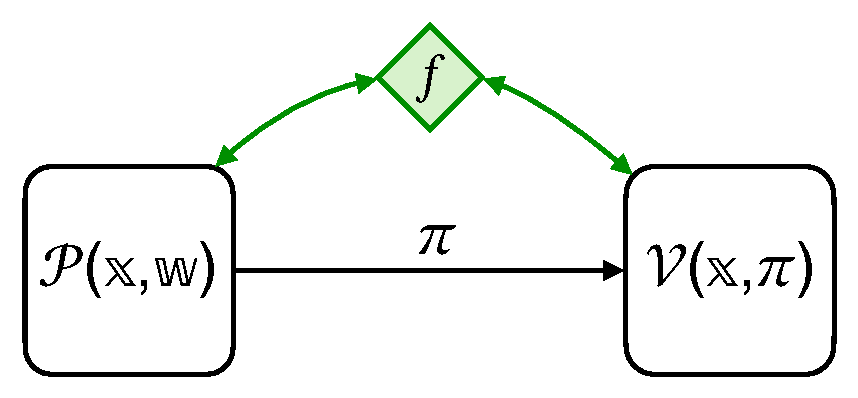
\includegraphics[width=\textwidth]{\FigureFolder/narg-diagram}
  \caption{}
  \label{figure:narg-diagram}
\end{subfigure}
\quad
\begin{subfigure}[b]{0.4\textwidth}
  \centering
  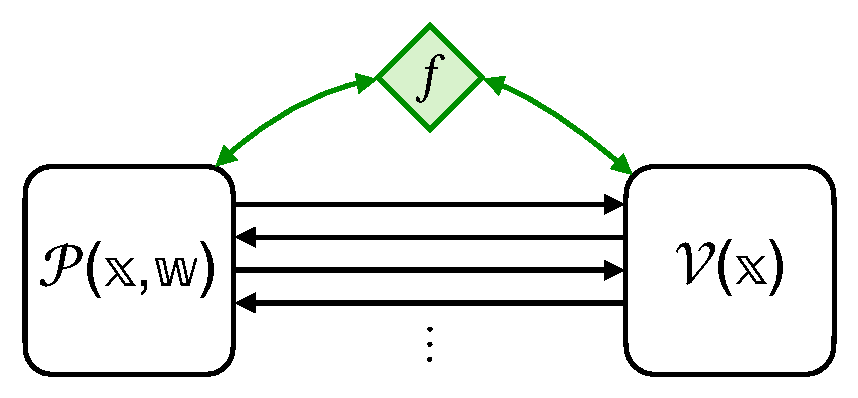
\includegraphics[width=\textwidth]{\FigureFolder/iarg-diagram}
  \caption{}
  \label{figure:iarg-diagram}
\end{subfigure}
\caption[Diagram of a NARG and an IARG.]{Diagram of a non-interactive argument (left) and an interactive argument (right), in the random oracle model. }
\label{figure:arg-diagrams}
\end{figure}

%%%%%%%%%%%%%%%%%%%%%%%%%%%%%%%%%%%%%%%%%%%%%%%%%%%%%%%%%%%%%%%%%%%%%%%%%%%%%%%
%%%%%%%%%%%%%%%%%%%%%%%%%%%%%%%%%%%%%%%%%%%%%%%%%%%%%%%%%%%%%%%%%%%%%%%%%%%%%%%
%%%%%%%%%%%%%%%%%%%%%%%%%%%%%%%%%%%%%%%%%%%%%%%%%%%%%%%%%%%%%%%%%%%%%%%%%%%%%%%
\section{Interactive arguments}
\label{section:iarg-basics}

The notion of a non-interactive argument can be relaxed to allow the argument prover and argument verifier to interact over some number of rounds. We introduce this relaxation because in this book we sometimes study simpler interactive protocols before studying non-interactive counterparts.

An \emph{interactive argument} (IARG) in the ROM is a tuple
\begin{equation*}
\IARGSymbol = \ARGSystem
\end{equation*}
where $\ARGProver$ is an oracle interactive algorithm known as the \emph{argument prover} and $\ARGVerifier$ is an oracle interactive algorithm known as the \emph{argument verifier}.

A random oracle $\ROFunction$ is sampled from the distribution $\RODistribution{\ROOutputSize}$, for a given output size $\ROOutputSize \in \Naturals$. Anyone, including the argument prover $\ARGProver$ and the argument verifier $\ARGVerifier$, can query $\ROFunction$. The argument prover $\ARGProver$ receives as input an instance $\Instance$ and witness $\Witness$, and the argument verifier $\ARGVerifier$ receives as input the instance $\Instance$. The argument prover $\ARGProver$ and argument verifier $\ARGVerifier$ interact over several rounds, and after this interaction the argument verifier $\ARGVerifier$ outputs a bit denoting whether to accept (the bit is $1$) or reject (the bit is $0$). See \Cref{figure:iarg-diagram} for a diagram.

We say that $\IARGSymbol = \ARGSystem$ is an interactive argument in the ROM for a relation $\Relation$ if it satisfies two main properties: \emph{completeness} and \emph{soundness}.
\begin{itemize}

  \item \textbf{Completeness.}
  Informally, for every instance-witness pair $(\Instance,\Witness) \in \Relation$, the (honest) argument prover $\ARGProver$ on input $(\Instance,\Witness)$ makes the argument verifier $\ARGVerifier$ on input $\Instance$ accept, with probability $1$. The probability here is taken over the choice of random oracle $\ROFunction$, as well as any randomness of $\ARGProver$ and of $\ARGVerifier$.

See \Cref{definition:iarg-completeness} below for a formal definition.

  \item \textbf{Soundness.}
  Informally, every malicious argument prover $\Malicious{\ARGProver}$ convinces the (honest) argument verifier $\ARGVerifier$ to accept an instance $\Instance \notin \GetLanguage{\Relation}$ with at most a small error probability $\ARGSoundnessError$ (over the choice of random oracle $\ROFunction$). The malicious argument prover $\Malicious{\ARGProver}$ may query the random oracle $\ROQueryBound$ for some given query bound $\ROQueryBound$, and is otherwise computationally unbounded.

Similarly to the case of a NARG, an important technical detail is how the instance $\Instance$ is chosen. In \Cref{definition:iarg-nonadaptive-soundness} below we provide a formal statement for non-adaptive soundness, and in \Cref{definition:iarg-adaptive-soundness} below we provide a formal statement for adaptive soundness.

\end{itemize}
Below we provide the definitions of completeness, non-adaptive soundness, and adaptive soundness. Given two interactive oracle algorithms $A$ and $B$, we use the notation $\ARGInteract{A}{B}$ to indicate the random variable that equals the output of $B$ after interacting with $A$, and where the probability is taken over any randomness used by $A$ or $B$ (as well as the random oracle given to $A$ and $B$).

\begin{ImportantDefinition}{completeness}{iarg-completeness}
An interactive argument $\IARGSymbol = \ARGSystem$ for a relation $\Relation$ is \defemph{(perfectly) complete} if for every output size $\ROOutputSize \in \Naturals$ of the random oracle and instance-witness pair $(\Instance,\Witness) \in \Relation$,
\begin{equation*}
\Pr\left[
\ARGInteract{\ARGProver^{\ROFunction}(\Instance,\Witness)}{\ARGVerifier^{\ROFunction}(\Instance)}=1
\GivenExperiment
\StateExperiment{
\ROFunction \gets \RODistribution{\ROOutputSize}
}
\right]
= 1
\enspace.
\end{equation*}
The probability is also over $\ROFunction$ and any randomness of the argument prover $\ARGProver$ and verifier $\ARGVerifier$.
\end{ImportantDefinition}

\begin{ImportantDefinition}{non-adaptive soundness}{iarg-nonadaptive-soundness}
An interactive argument $\IARGSymbol = \ARGSystem$ for a relation $\Relation$ has \defemph{non-adaptive soundness error} $\ARGNASoundnessError$ if for every output size $\ROOutputSize \in \Naturals$ of the random oracle, query bound $\ROQueryBound \in \Naturals$, $\ROQueryBound$-query malicious argument prover $\Malicious{\ARGProver}$, and instance $\Instance \notin \GetLanguage{\Relation}$,
\begin{equation*}
\Pr\left[
\ARGInteract{\Malicious{\ARGProver}^{\ROFunction}}{\ARGVerifier^{\ROFunction}(\Instance)}=1
\GivenExperiment
\StateExperiment{
\ROFunction \gets \RODistribution{\ROOutputSize}
}
\right]
\leq
\ARGNASoundnessError(\ROOutputSize,\ROQueryBound,\Instance)
\enspace.
\end{equation*}
The probability is taken over $\ROFunction$ and any randomness of the argument verifier $\ARGVerifier$.
\end{ImportantDefinition}

\begin{ImportantDefinition}{adaptive soundness}{iarg-adaptive-soundness}
An interactive argument $\IARGSymbol = \ARGSystem$ for a relation $\Relation$ has \defemph{adaptive soundness error} $\ARGSoundnessError$ if for every output size $\ROOutputSize \in \Naturals$ of the random oracle, query bound $\ROQueryBound \in \Naturals$, $\ROQueryBound$-query malicious argument prover $\Malicious{\ARGProver}$, and instance size bound $\InstanceSize \in \Naturals$,
\begin{equation*}
\Pr\left[
\begin{array}{l}
\SomeSize{\Instance} \leq \InstanceSize \\
\land\;\Instance \notin \GetLanguage{\Relation} \\
\land\;\ARGInteract{\Malicious{\ARGProver}^{\ROFunction}(\ROAdvState)}{\ARGVerifier^{\ROFunction}(\Instance)}=1
\end{array}
\GivenExperiment
\StateExperiment{
\ROFunction \gets \RODistribution{\ROOutputSize} \\
(\Instance,\ROAdvState) \gets \Malicious{\ARGProver}^{\ROFunction}
}
\right]
\leq
\ARGSoundnessError(\ROOutputSize,\ROQueryBound,\InstanceSize)
\enspace.
\end{equation*}
The probability is taken over $\ROFunction$ and any randomness of the argument verifier $\ARGVerifier$.
\end{ImportantDefinition}

\parhead{Public coins}
We study interactive arguments that are \emph{public-coin}, which means that each message of the argument verifier $\ARGVerifier$ is a random message. A non-interactive argument is trivially public coin because, in this case, the argument verifier does not send any messages.

\begin{definition}
\label{definition:arg-public-coin}
$\IARGSymbol = \ARGSystem$ is \defemph{public-coin} if each message $\IARGVerifierRandomMessage_{\RoundIndex}$ by the argument verifier $\ARGVerifier$ is a random binary string of some prescribed size $\IARGRandomnessComplexity_{\RoundIndex}$. In this case, the decision bit of the argument verifier $\ARGVerifier$ is a function only of the random oracle $\ROFunction$, the instance $\Instance$, and the transcript of interaction $(\IARGProverMessage_{1},\IARGVerifierRandomMessage_{1},\dots,\IARGProverMessage_{\IARGRoundComplexity},\IARGVerifierRandomMessage_{\IARGRoundComplexity})$; we denote this bit by $\ARGVerifier^{\ROFunction}\big(\IARGVerifierInput\big)$.
\end{definition}

%%%%%%%%%%%%%%%%%%%%%%%%%%%%%%%%%%%%%%%%%%%%%%%%%%%%%%%%%%%%%%%%%%%%%%%%%%%%%%%
%%%%%%%%%%%%%%%%%%%%%%%%%%%%%%%%%%%%%%%%%%%%%%%%%%%%%%%%%%%%%%%%%%%%%%%%%%%%%%%
%%%%%%%%%%%%%%%%%%%%%%%%%%%%%%%%%%%%%%%%%%%%%%%%%%%%%%%%%%%%%%%%%%%%%%%%%%%%%%%
\section{Efficiency measures}
\label{section:arg-efficiency-measures}

We study several efficiency measures for interactive and non-interactive arguments. All measures can be functions of the output size $\ROOutputSize$ of the random oracle and of the instance $\Instance$ (or the instance size bound $\InstanceSize$).

\parhead{Prover cost}
We denote by $\ARGTimeP$ the running time of the prover algorithm $\ARGProver$, and by $\ARGQueryP$ the number of queries that it makes to the random oracle (regardless of their size). If $\ARGProver$ is part of an interactive argument then $\ARGProver$ is an interactive algorithm, and these costs refer to the total running time and number of queries across all rounds of interaction.

\parhead{Verifier cost}
We denote by $\ARGTimeV$ the running time of the verifier algorithm $\ARGVerifier$, and by $\ARGQueryV$ the number of queries that it makes to the random oracle (regardless of their size). If $\ARGVerifier$ is part of an interactive argument then $\ARGVerifier$ is an interactive algorithm, and these costs refer to the total running time and number of queries across all rounds of interaction.

\parhead{Communication}
In the case of an \emph{interactive} argument, we denote by $\ARGPCommunication$ the total number of bits sent by the argument prover $\ARGProver$ (across all rounds of interaction) and we denote by $\ARGVCommunication$ the total number of bits sent by the argument verifier $\ARGVerifier$ (across all rounds of interaction). In particular, the transcript of interaction between $\ARGProver$ and $\ARGVerifier$ consists of $\ARGCommunication = \ARGPCommunication+\ARGVCommunication$ bits.

In the case of a \emph{non-interactive} argument, there is a single message $\ARGString$ from the argument prover $\ARGProver$ and no messages from the argument verifier $\ARGVerifier$, which means that $\ARGVCommunication=0$. In this case we denote by $\ARGLength=\ARGPCommunication$ the size of the argument string $\ARGString$.

%%%%%%%%%%%%%%%%%%%%%%%%%%%%%%%%%%%%%%%%%%%%%%%%%%%%%%%%%%%%%%%%%%%%%%%%%%%%%%%
%%%%%%%%%%%%%%%%%%%%%%%%%%%%%%%%%%%%%%%%%%%%%%%%%%%%%%%%%%%%%%%%%%%%%%%%%%%%%%%
%%%%%%%%%%%%%%%%%%%%%%%%%%%%%%%%%%%%%%%%%%%%%%%%%%%%%%%%%%%%%%%%%%%%%%%%%%%%%%%
\section{Succinct arguments}
\label{section:arg-succinctness}

A central goal of the non-interactive arguments described in this book is \textbf{succinctness}, which is a spectrum of efficiency goals with differing strengths. Briefly, succinctness can refer to \emph{small communication} or, additionally, \emph{fast verification}. We elaborate on these notions below.

\parhead{Baseline: the trivial argument system}
Every relation $\Relation$ has a trivial proof system: the prover sends the witness, and the verifier checks the validity of the witness. Expressing this as a trivial non-interactive argument yields two main baselines that enable defining succinctness.

The (honest) argument prover, given as input an instance $\Instance$ and witness $\Witness$, outputs the argument string $\ARGString \DefineEqual \Witness$; and the argument verifier, given as input the instance $\Instance$ and argument string $\ARGString$, checks that $(\Instance,\ARGString) \in \Relation$. This non-interactive argument does not use the random oracle, and has perfect completeness and zero soundness error. (As discussed in \Cref{remark:trivial-narg-not-zk}, the trivial non-interactive argument is not zero knowledge; but this is irrelevant to the present discussion on efficiency.)

The trivial non-interactive argument for $\Relation$ sets two important baselines.
\begin{itemize}[noitemsep]
  \item The argument size is the witness size: $\ARGLength \DefineEqual \BitSize{\Witness}$.
  \item The verification time is the time to decide the relation: $\ARGTimeV \DefineEqual \RelationTime(\Instance,\Witness)$.
\end{itemize}
Succinctness covers several goals that involve doing better in argument size or verification time.

\parhead{Succinctness in communication}
Argument systems that achieve communication that is better than the witness size are considered \emph{succinct in communication}. The relevant metric for a non-interactive argument is the argument size $\ARGLength$, while the relevant metric for an interactive argument is the prover-to-verifier communication $\ARGPCommunication$ (or perhaps even the total communication $\ARGCommunication = \ARGPCommunication+\ARGVCommunication$).

But what does \DoQuote{better than the witness size} mean?

A modest goal is communication that is sublinear in witness size while allowing for some dependence on the output size of the random oracle: $\poly(\ROOutputSize) \cdot o(\BitSize{\Witness})$.\footnote{The \DoQuote{$o(n)$} notation includes all functions $g(n)$ such that, for every $c>0$, $g(n) \leq c \cdot n$ for large enough $n$.} Even better is a (poly)logarithmic dependence on witness size while again allowing for some dependence on the output size of the random oracle: $\poly(\ROOutputSize,\log\BitSize{\Witness})$. These are not the only regimes of interest, and in fact usually it is helpful to express the communication succinctness of a succinct argument as an explicit expression of the relevant parameters. Overall, the goal is to achieve $\ARGLength \ll \BitSize{\Witness}$.

\parhead{Succinctness in verification}
Argument systems that achieve verifier time that is better than the time to decide the relation are considered \emph{succinct in verification}. The relevant metric for both interactive arguments and non-interactive arguments is the time $\ARGTimeV$ of the argument verifier.

Again, we can ask \DoQuote{what does better than the time to decide the relation} mean?

Similarly to above, a modest goal is a verification time that is sublinear in the relation decision time while allowing for some dependence on the output size of the random oracle: $\poly(\ROOutputSize) \cdot o(\RelationTime(\Instance,\Witness))$. Even better is a (poly)logarithmic dependence on the relation decision time while again allowing for some dependence on the output size of the random oracle: $\poly(\ROOutputSize,\log \RelationTime(\Instance,\Witness))$. It is helpful to express the verification succinctness of a succinct argument as an explicit expression of the relevant parameters, and overall the goal is to achieve $\ARGTimeV \ll \RelationTime(\Instance,\Witness)$.

Observe that the verifier time of an argument system is an upper bound on communication ($\ARGTimeV \geq \ARGLength$), which means that succinctness in verification usually implies (some form of) succinctness in communication. In constructions of succinct arguments, the achieved communication complexity is often better than the upper bound implied by the verifier time.

\parhead{Special case: no witnesses}
Relations $\Relation$ where there are no witnesses are a notable special case. In this case $\Relation$ can be viewed as a language $\Language$, and the trivial non-interactive argument above collapses to a solitary verifier: the argument verifier decides on its own whether the input instance $\Instance$ is $\Language$, without receiving anything from the argument prover (as there are no witnesses).

The baseline of witness size for $\Language$ is zero, so it is \emph{not meaningful to consider succinctness in communication}. Indeed, sending any argument string is more expensive in communication than sending nothing. So, there is no way to improve in communication over the baseline.

On the other hand, succinctness in verification is meaningful, namely, the goal is to achieve an argument verifier that runs in time better than the time $\LanguageTime(\Instance)$ to decide membership of $\Instance$ in the language $\Language$. As before, one can consider a modest goal of time $\poly(\ROOutputSize) \cdot o(\LanguageTime(\Instance))$, aim for a stronger goal such as $\poly(\ROOutputSize,\log \LanguageTime(\Instance))$, or, more generally, achieve $\ARGTimeV \ll \LanguageTime(\Instance)$.

A common example of a relation with no witnesses supported by succinct arguments is $\DTIME(T)$, which consists of all (deterministic) machines that accept in time $T$. It is the analogue of the relation $\NTIME(T)$ but without witnesses.

\parhead{Terminology for succinct arguments}
An interactive argument or non-interactive argument is generally called \textbf{succinct} if any of the above improvements over baseline are met. Moreover, the acronym \textbf{SNARG} stands for a succinct \emph{non-interactive} argument. In particular, in this book we study constructions of SNARGs in the random oracle model (ROM). If a SNARG satisfies knowledge soundness then it may be called a \textbf{SNARK}, and if it additionally satisfies zero knowledge it may be called a \textbf{zkSNARK}.

In practice, the random oracle is heuristically instantiated via a cryptographic hash function (see \Cref{section:rom-as-concrete-hash}), which yields an argument system in the \emph{standard model} (what cryptographers call a setting without oracles). The specification of the hash function can then be viewed as the public parameters, or \emph{setup}, of the argument system. Making the choice of cryptographic hash function typically does not involve any secret randomness, in which case the SNARG is said to have a \textbf{transparent setup} (or \textbf{public-coin setup}). Thus, for example, a zkSNARK in the ROM becomes a \textbf{zkSNARK with a transparent setup}, when the random oracle is heuristically instantiated. A notable example of SNARGs in the ROM are \textbf{STARKs} (scalable transparent arguments of knowledge), whose security in the ROM is covered by the material discussed in this book.

%%%%%%%%%%%%%%%%%%%%%%%%%%%%%%%%%%%%%%%%%%%%%%%%%%%%%%%%%%%%%%%%%%%%%%%%%%%%%%%
%%%%%%%%%%%%%%%%%%%%%%%%%%%%%%%%%%%%%%%%%%%%%%%%%%%%%%%%%%%%%%%%%%%%%%%%%%%%%%%
%%%%%%%%%%%%%%%%%%%%%%%%%%%%%%%%%%%%%%%%%%%%%%%%%%%%%%%%%%%%%%%%%%%%%%%%%%%%%%%
%%%%%%%%%%%%%%%%%%%%%%%%%%%%%%%%%%%%%%%%%%%%%%%%%%%%%%%%%%%%%%%%%%%%%%%%%%%%%%%
\chapter{Additional security definitions}
\label{chapter:narg-advanced}

In applications, arguments are often required to satisfy additional security definitions beyond completeness and soundness. Since non-interactive arguments (NARGs) are the focus of this book, below we provide these additional security definitions only for non-interactive arguments.
\begin{itemize}[noitemsep]
  \item In \Cref{section:narg-knowledge-soundness} we discuss \emph{knowledge soundness}.
  \item In \Cref{section:narg-zero-knowledge} we discuss \emph{zero knowledge}.
\end{itemize}
In this book we describe how to achieve these additional security definitions for each NARG construction that we study.

%%%%%%%%%%%%%%%%%%%%%%%%%%%%%%%%%%%%%%%%%%%%%%%%%%%%%%%%%%%%%%%%%%%%%%%%%%%%%%%
%%%%%%%%%%%%%%%%%%%%%%%%%%%%%%%%%%%%%%%%%%%%%%%%%%%%%%%%%%%%%%%%%%%%%%%%%%%%%%%
%%%%%%%%%%%%%%%%%%%%%%%%%%%%%%%%%%%%%%%%%%%%%%%%%%%%%%%%%%%%%%%%%%%%%%%%%%%%%%%
\section{Knowledge soundness}
\label{section:narg-knowledge-soundness}

The soundness property (see \Cref{definition:narg-nonadaptive-soundness,definition:narg-adaptive-soundness}) states that every malicious argument prover cannot convince the argument verifier to accept instances not in the language (associated to the relation), except for a small error probability.

\emph{Knowledge soundness} strengthens this by requiring that whenever an argument prover convinces the argument verifier to accept then, except for a small error probability, the argument prover \DoQuote{knows} a valid witness that shows that the instance is in the language.\footnote{Arguments that satisfy this property are sometimes called \emph{proofs of knowledge} or, if emphasizing the fact that security holds only against suitably bounded malicious provers, \emph{arguments of knowledge}.}

If the instance is in the language, then a witness exists and so can be found, for example, via brute-force search (an inefficient procedure). Knowledge soundness requires that there exists an efficient procedure, called the \emph{extractor}, that finds a witness from the argument prover (thereby demonstrating the malicious prover's knowledge).

There are different flavors of knowledge soundness, depending on how the extractor accesses information about the malicious prover. Below we consider two flavors, a stronger one and a weaker one. Both are \emph{adaptive}, in that the argument prover can use the random oracle to choose the instance for which to provide the argument string.\footnote{Corresponding non-adaptive relaxations can be straightforwardly derived from these definitions.}

\parhead{Straightline knowledge soundness}
The definition below captures a flavor of knowledge soundness that is known as \emph{straightline}, because the extractor only needs information associated to a single execution of the argument prover. In more detail, the extractor finds the witness given only the argument prover's output and query-answer trace with the random oracle.\footnote{In particular, since the extraction procedure does not \DoQuote{change} the random oracle, this property is said to hold in the \emph{non-programmable} ROM.} This strong notion is particularly useful in a multitude of settings.

\begin{ImportantDefinition}{straightline knowledge soundness}{adaptive-straightline-knowledge-soundness}
A non-interactive argument $\NARGSymbol=\ARGSystem$ for a relation $\Relation$ has \defemph{straightline knowledge soundness error $\ARGKnowledgeError$} if there exists a polynomial-time deterministic algorithm $\ARGExtractor$ (the \emph{extractor}) such that for every output size $\ROOutputSize \in \Naturals$ of the random oracle, query bound $\ROQueryBound \in \Naturals$, $\ROQueryBound$-query deterministic argument prover $\Malicious{\ARGProver}$, and instance size bound $\InstanceSize \in \Naturals$,
\begin{equation*}
\Pr\left[
\begin{array}{l}
\SomeSize{\Instance} \leq \InstanceSize \\
\land\;(\Instance,\Witness) \notin \Relation \\
\land\;\ARGVerifier^{\ROFunction}(\Instance,\ARGString)=1
\end{array}
\GivenExperiment
\StateExperiment{
\ROFunction \gets \RODistribution{\ROOutputSize} \\
\ROOutputAndTrace{\ROFunction}{\Malicious{\ARGProver}}{\ROTrace}{(\Instance,\ARGString)} \\
\Witness \gets \ARGExtractor(\Instance,\ARGString,\ROTrace)
}
\right]
\leq
\ARGKnowledgeError(\ROOutputSize,\ROQueryBound,\InstanceSize)
\enspace.
\end{equation*}
\end{ImportantDefinition}

\parhead{Rewinding knowledge soundness}
The definition below captures a relaxation known as \emph{rewinding}, where the extraction additionally receives the argument prover (as a black-box). This enables the extractor to re-run the argument prover multiple times on inputs of its choice. The extractor is also given access to the random oracle, for example to facilitate these re-runs. The extractor error is additionally allowed to the depend on failure probability of the argument prover (in convincing the verifier), which is also defined below.

\begin{definition}
\label{definition:argument-failure-probability}
Let $\NARGSymbol=\ARGSystem$ be a non-interactive argument. A deterministic argument prover $\Malicious{\ARGProver}$ has \defemph{failure probability $\ProverFailureProbability{\Malicious{\ARGProver}}$} if for every output size $\ROOutputSize \in \Naturals$ of the random oracle and instance size bound $\InstanceSize \in \Naturals$,
\begin{equation*}
\Pr\left[
\begin{array}{l}
  \SomeSize{\Instance} > \InstanceSize \\
  \lor \;\ARGVerifier^{\ROFunction}(\Instance,\ARGString)=0
\end{array}
\GivenExperiment
\StateExperiment{
  \ROFunction \gets \RODistribution{\ROOutputSize} \\
  (\Instance,\ARGString) \gets \Malicious{\ARGProver}^{\ROFunction}
}
\right]
\leq
\ProverFailureProbability{\Malicious{\ARGProver}}(\ROOutputSize,\InstanceSize)
\enspace.
\end{equation*}
\end{definition}

\begin{ImportantDefinition}{rewinding knowledge soundness}{adaptive-rewinding-knowledge-soundness}
A non-interactive argument $\NARGSymbol=\ARGSystem$ for a relation $\Relation$ has \defemph{rewinding knowledge soundness error $\ARGKnowledgeError$ with extraction time $\ARGKnowledgeTime$} if there exists a probabilistic algorithm $\ARGExtractor$ (the \emph{extractor}) such that for every output size $\ROOutputSize \in \Naturals$ of the random oracle, query bound $\ROQueryBound \in \Naturals$, $\ROQueryBound$-query deterministic argument prover $\Malicious{\ARGProver}$ with failure probability $\ProverFailureProbability{\Malicious{\ARGProver}}$ and running time $\ProverRunningTime{\Malicious{\ARGProver}}$, and instance size bound $\InstanceSize \in \Naturals$,
\begin{equation*}
\Pr\left[
\begin{array}{l}
\SomeSize{\Instance} \leq \InstanceSize \\
\land\;(\Instance,\Witness) \notin \Relation \\
\land\;\ARGVerifier^{\ROFunction}(\Instance,\ARGString)=1
\end{array}
\GivenExperiment
\StateExperiment{
\ROFunction \gets \RODistribution{\ROOutputSize} \\
\ROOutputAndTrace{\ROFunction}{\Malicious{\ARGProver}}{\ROTrace}{(\Instance,\ARGString)} \\
\Witness \gets \ARGExtractor^{\ROFunction}(\Instance,\ARGString,\ROTrace,\BlackBox{\Malicious{\ARGProver}})
}
\right]
\leq
\ARGKnowledgeError\left(\ROOutputSize,\ROQueryBound,\InstanceSize,\ProverFailureProbability{\Malicious{\ARGProver}}(\ROOutputSize,\InstanceSize)\right)
\enspace.
\end{equation*}
Moreover, $\ARGExtractor$ runs in expected time $\ARGKnowledgeTime\left(\ROOutputSize,\ROQueryBound,\InstanceSize,\ProverFailureProbability{\Malicious{\ARGProver}}(\ROOutputSize,\InstanceSize),\ProverRunningTime{\Malicious{\ARGProver}}(\ROOutputSize,\InstanceSize)\right)$ (over the given inputs and internal randomness).
\end{ImportantDefinition}

\Cref{definition:adaptive-straightline-knowledge-soundness} implies \Cref{definition:adaptive-rewinding-knowledge-soundness} because the two properties are the same except that in the latter the extractor is randomized and also has access to the malicious argument prover.

\begin{remark}[probabilistic provers]
\label{remark:probabilistic-argument-provers}
The knowledge soundness definitions are stated for \emph{deterministic} provers for simplicity. These imply definitions for probabilistic provers, as we now explain.
\begin{itemize}[noitemsep]
  \item The definition of \emph{straightline} knowledge soundness for probabilistic argument provers $\Malicious{\ARGProver}$ is the same as in \Cref{definition:adaptive-straightline-knowledge-soundness} except that the execution $\ROOutputAndTrace{\ROFunction}{\Malicious{\ARGProver}}{\ROTrace}{(\Instance,\ARGString)}$ in the experiment also takes into account the randomness of $\Malicious{\ARGProver}$.
  \item The definition of \emph{rewinding} knowledge soundness for probabilistic argument provers $\Malicious{\ARGProver}$ is a slight variant of \Cref{definition:adaptive-rewinding-knowledge-soundness}. Namely, letting $\ARGProverRandomnessSet$ be the set of possible random strings for $\Malicious{\ARGProver}$, the experiment is modified to explicitly account for the randomness of $\Malicious{\ARGProver}$ as follows:
\begin{align*}
\left[
\StateExperiment{
  \ROFunction \gets \RODistribution{\ROOutputSize} \\
  \ARGProverRandomness \gets \ARGProverRandomnessSet \\
  \ShortExecutionOver{(\Instance,\ARGString)}{\Malicious{\ARGProver}^{\ROFunction}(\ARGProverRandomness)}{\ROTrace} \\
  \Witness \gets \ARGExtractor^{\ROFunction}(\Instance,\ARGString,\ROTrace,\BlackBox{\Malicious{\ARGProver}(\ARGProverRandomness)})
}
\right]
\end{align*}
The extractor $\ARGExtractor$ has black-box access to the argument prover $\Malicious{\ARGProver}$ with its randomness $\ARGProverRandomness$ hardcoded. The rest of the definition is the same.
\end{itemize}
In both of the above cases, the knowledge error and extractor time bounds for probabilistic provers are directly implied by the corresponding bounds for deterministic provers. Indeed, the probabilistic argument prover $\Malicious{\ARGProver}$ can be expressed as $\Cardinality{\ARGProverRandomnessSet}$ deterministic argument provers, each corresponding to a different choice of randomness $\ARGProverRandomness \in \ARGProverRandomnessSet$ (and all with the same query bound). Since the knowledge soundness definition applies to all deterministic provers, the error bound $\ARGKnowledgeError$ holds for each of these $\Cardinality{\ARGProverRandomnessSet}$ provers. The error of $\Malicious{\ARGProver}$ is the average of these errors, and hence is upper bounded by $\ARGKnowledgeError$. Similarly for the expected running time of the extractor: the upper bound $\ARGKnowledgeTime$ holds for each of the $\Cardinality{\ARGProverRandomnessSet}$ deterministic provers; the expected running time of $\ARGExtractor$ for $\Malicious{\ARGProver}$ is the average of the expected running times for the deterministic provers, and this average is upper bounded by $\ARGKnowledgeTime$.
\end{remark}

\begin{remark}[monotonicity of $\ARGKnowledgeError$]
\label{remark:monotonicity-of-knowledge-error}
The rewinding knowledge soundness error $\ARGKnowledgeError$ depends on the parameters $\ROOutputSize,\ROQueryBound,\InstanceSize,\ProverFailureProbability{\Malicious{\ARGProver}}$. Throughout this book, we assume that $\ARGKnowledgeError$ is (weakly) monotone increasing with respect to these parameters. Except for contrived examples, known error functions $\ARGKnowledgeError$ behave this way. For example, if $\ROQueryBound$ increases then we expect $\ARGKnowledgeError$ to not decrease because the argument prover has more power (it can ask more queries to the random oracle). Moreover, if $\ProverFailureProbability{\Malicious{\ARGProver}}$ increases then we expect $\ARGKnowledgeError$ to not decrease because knowledge extraction becomes harder if the probability that the argument prover convinces the argument verifier decreases.
\end{remark}

\begin{remark}
\label{remark:simple-narg-not-knowledge-sound}
It is straightforward to construct a non-interactive argument that is \emph{not} knowledge sound (for any reasonable definition of knowledge soundness including the ones we give). Let $\mathcal{G} = \{g_{\ell} \colon \Bits^{\ell} \to \Bits^{\ell}\}_{\ell \in \Naturals}$ be a collection of permutations and consider the relation $\Relation \DefineEqual \{(\Instance,\Witness) : g_{\BitSize{\Instance}}(\Witness)=\Instance \}$. Note that $\GetLanguage{\Relation}=\Bits^{*}$, that is, the language associated to $\Relation$ is trivial (it contains all binary strings). Consider the following trivial non-interactive argument for $\Relation$:
\begin{itemize}[noitemsep]
  \item the argument prover $\ARGProver^{\ROFunction}(\Instance,\Witness)$ outputs $\ARGString \DefineEqual \bot$ (an empty string); and
  \item the argument verifier $\ARGVerifier^{\ROFunction}(\Instance,\ARGString)$ always accepts.
\end{itemize}
This non-interactive argument is perfectly complete and perfectly sound (since there are no instances not in the language).

On the other hand, any algorithm that receives as input an instance $\Instance$ and outputs a witness $\Witness$ such that $(\Instance,\Witness) \in \Relation$ has found a preimage of $\Instance$ under $g_{\BitSize{\Instance}}$. Additionally, receiving as input information about a malicious prover (e.g., its query-answer trace or even the code of the malicious prover itself) does not provide any help towards inverting $g_{\BitSize{\Instance}}$ because a malicious argument prover can convince the argument verifier without making any queries or producing any argument string.

Hence, if inverting functions from the collection of permutations $\mathcal{G}$ is hard (e.g., $\mathcal{G}$ is a collection of one-way permutations), then no efficient algorithm can find a witness for the given instance with non-negligible probability (in $\BitSize{\Instance}$). We conclude that the above non-interactive argument does not satisfy knowledge soundness.
\end{remark}

\parhead{Equivalent definition of rewinding knowledge soundness}
We use a definition equivalent to \Cref{definition:adaptive-rewinding-knowledge-soundness} when establishing rewinding knowledge soundness for non-interactive arguments. Below we discuss this alternative definition, which in this book is more convenient to work with. Briefly, the extractor $\ARGExtractor$ receives as input the query-answer trace of the argument verifier, instead of receiving query access to the random oracle.

\begin{ImportantDefinition}{rewinding knowledge soundness}{adaptive-rewinding-knowledge-soundness-verifier-trace}
A non-interactive argument $\NARGSymbol=\ARGSystem$ for a relation $\Relation$ has \defemph{rewinding knowledge soundness error $\ARGKnowledgeError$ with extraction time $\ARGKnowledgeTime$} if there exists a probabilistic algorithm $\ARGExtractor$ (the \emph{extractor}) such that for every output size $\ROOutputSize \in \Naturals$ of the random oracle, query bound $\ROQueryBound \in \Naturals$, $\ROQueryBound$-query deterministic argument prover $\Malicious{\ARGProver}$ with failure probability $\ProverFailureProbability{\Malicious{\ARGProver}}$ and running time $\ProverRunningTime{\Malicious{\ARGProver}}$, and instance size bound $\InstanceSize \in \Naturals$,
\begin{equation*}
\Pr\left[
\begin{array}{l}
  \SomeSize{\Instance} \leq \InstanceSize \\
  \land\;(\Instance,\Witness) \notin \Relation \\
  \land\;\DecisionBit=1
\end{array}
\GivenExperiment
\StateExperiment{
  \ROFunction \gets \RODistribution{\ROOutputSize} \\
  \ROOutputAndTrace{\ROFunction}{\Malicious{\ARGProver}}{\ROTrace}{(\Instance,\ARGString)} \\
  \DecisionBit \xleftarrow{\ROTraceVerifier} \ARGVerifier^{\ROFunction}(\Instance,\ARGString) \\
  \Witness \gets \ARGExtractor(\Instance,\ARGString,\ROTrace,\ROTraceVerifier,\BlackBox{\Malicious{\ARGProver}})
}
\right]
\leq
\ARGKnowledgeError\left(\ROOutputSize,\ROQueryBound,\InstanceSize,\ProverFailureProbability{\Malicious{\ARGProver}}(\ROOutputSize,\InstanceSize)\right)
\enspace.
\end{equation*}
Moreover, $\ARGExtractor$ runs in expected time $\ARGKnowledgeTime\left(\ROOutputSize,\ROQueryBound,\InstanceSize,\ProverFailureProbability{\Malicious{\ARGProver}}(\ROOutputSize,\InstanceSize),\ProverRunningTime{\Malicious{\ARGProver}}(\ROOutputSize,\InstanceSize)\right)$ (over the given inputs and internal randomness).
\end{ImportantDefinition}

Below we prove that \Cref{definition:adaptive-rewinding-knowledge-soundness} and \Cref{definition:adaptive-rewinding-knowledge-soundness-verifier-trace} are equivalent. Here we provide some intuition for this equivalence. What use is the random oracle $\ROFunction$ to the extractor $\ARGExtractor$? Information about queries performed by the malicious argument prover $\Malicious{\ARGProver}$ are included in the trace (an input to $\ARGExtractor$), so $\ARGExtractor$ does not need to access $\ROFunction$ for such queries. Queries not performed by $\Malicious{\ARGProver}$ or (honest) argument verifier $\ARGVerifier$ are random and independent of all inputs given to $\ARGExtractor$, which means that $\ARGExtractor$ can sample the answer to these queries without access to $\ROFunction$. Hence, the only queries that are potentially \DoQuote{valuable} to $\ARGExtractor$ are those performed by $\ARGVerifier$ (and not by $\Malicious{\ARGProver}$). The alternative definition provides the query-answer trace of $\ARGVerifier$ as an input to $\ARGExtractor$ to cover this case.

\begin{claim}
\label{claim:narg-knowledge-soundness-equivalent-definitions}
A non-interactive argument $\NARGSymbol=\ARGSystem$ for a relation $\Relation$ has knowledge soundness error $\ARGKnowledgeError$ with respect to definition \Cref{definition:adaptive-rewinding-knowledge-soundness} if and only if it has knowledge soundness error $\ARGKnowledgeError$ with respect to definition \Cref{definition:adaptive-rewinding-knowledge-soundness-verifier-trace}.
\end{claim}

\begin{proof}
We prove each direction of the claim separately.

\parhead{\Cref{definition:adaptive-rewinding-knowledge-soundness-verifier-trace} $\implies$ \Cref{definition:adaptive-rewinding-knowledge-soundness}}

Suppose that $\NARGSymbol$ has knowledge soundness error $\ARGKnowledgeError$ with respect to \Cref{definition:adaptive-rewinding-knowledge-soundness-verifier-trace}, and let $\ARGExtractor'$ be its extractor. We show that $\NARGSymbol$ has knowledge soundness error $\ARGKnowledgeError$ with respect to \Cref{definition:adaptive-rewinding-knowledge-soundness}, using the below extractor $\ARGExtractor$.
\begin{itemize}[noitemsep]
\item[] $\ARGExtractor^{\ROFunction}(\Instance,\ARGString,\ROTrace,\BlackBox{\Malicious{\ARGProver}})$:
\begin{enumerate}[nolistsep]
  \item Compute $\DecisionBit \xleftarrow{\ROTraceVerifier} \ARGVerifier^{\ROFunction}(\Instance,\ARGString)$.
  \item Compute $\Witness \gets \ARGExtractor'(\Instance,\ARGString,\ROTrace,\ROTraceVerifier,\BlackBox{\Malicious{\ARGProver}})$.
  \item Output $\Witness$.
\end{enumerate}
\end{itemize}
If $\ARGKnowledgeTime'$ is the running time of $\ARGExtractor'$ and $\ARGTimeV$ is the running time of $\ARGVerifier$, then the running time of $\ARGExtractor$ is at most $\ARGKnowledgeTime'(\ROOutputSize,\ROQueryBound,\InstanceSize,\ProverFailureProbability{\Malicious{\ARGProver}}(\ROOutputSize,\InstanceSize),\ProverRunningTime{\Malicious{\ARGProver}}(\ROOutputSize,\InstanceSize)) + \ARGTimeV$.

Next we upper bound the knowledge soundness error. By definition of $\ARGExtractor$,
\begin{align*}
&
\Pr\left[
\begin{array}{l}
  \SomeSize{\Instance} \leq \InstanceSize \\
  \land\;(\Instance,\Witness) \notin \Relation \\
  \land\;\ARGVerifier^{\ROFunction}(\Instance,\ARGString)=1
\end{array}
\GivenExperiment
\StateExperiment{
  \ROFunction \gets \RODistribution{\ROOutputSize} \\
  \ROOutputAndTrace{\ROFunction}{\Malicious{\ARGProver}}{\ROTrace}{(\Instance,\ARGString)} \\
  \Witness \gets \ARGExtractor^{\ROFunction}(\Instance,\ARGString,\ROTrace,\BlackBox{\Malicious{\ARGProver}})
}
\right]
\\ & \leq
\Pr\left[
\begin{array}{l}
  \SomeSize{\Instance} \leq \InstanceSize \\
  \land\;(\Instance,\Witness) \notin \Relation \\
  \land\;\DecisionBit=1
\end{array}
\GivenExperiment
\StateExperiment{
  \ROFunction \gets \RODistribution{\ROOutputSize} \\
  \ROOutputAndTrace{\ROFunction}{\Malicious{\ARGProver}}{\ROTrace}{(\Instance,\ARGString)} \\
  \DecisionBit \xleftarrow{\ROTraceVerifier} \ARGVerifier^{\ROFunction}(\Instance,\ARGString) \\
  \Witness \gets \ARGExtractor'(\Instance,\ARGString,\ROTrace,\ROTraceVerifier,\BlackBox{\Malicious{\ARGProver}})
}
\right]
\\ & =
\ARGKnowledgeError(\ROOutputSize,\ROQueryBound,\InstanceSize,\ProverFailureProbability{\Malicious{\ARGProver}}(\ROOutputSize,\InstanceSize))
\enspace.
\end{align*}

\parhead{\Cref{definition:adaptive-rewinding-knowledge-soundness} $\implies$ \Cref{definition:adaptive-rewinding-knowledge-soundness-verifier-trace}}
Suppose that $\NARGSymbol$ has knowledge soundness error $\ARGKnowledgeError$ with respect to \Cref{definition:adaptive-rewinding-knowledge-soundness}, and let $\ARGExtractor$ be its extractor. We show that $\NARGSymbol$ has knowledge soundness error $\ARGKnowledgeError$ with respect to \Cref{definition:adaptive-rewinding-knowledge-soundness-verifier-trace}, using the below extractor $\ARGExtractor'$.
\begin{itemize}[noitemsep]
\item[] $\ARGExtractor'(\Instance,\ARGString,\ROTrace,\ROTraceVerifier,\BlackBox{\Malicious{\ARGProver}})$:
\begin{enumerate}[nolistsep]
  \item Lazily sample an oracle $\Lazy{\ROFunction}' \gets \RODistribution{\ROOutputSize}$.
  \item Define $\Lazy{\ROFunction}'_{\ROTrace,\ROTraceVerifier}(\ROQuery) \DefineEqual
  \begin{cases}
    \ROAnswer & \text{if $(\ROQuery,\ROAnswer) \in \ROTrace \cup \ROTraceVerifier$}\\
    \Lazy{\ROFunction'}(\ROQuery) & \text{otherwise}
  \end{cases}$.
  \item Output $\Witness \gets \ARGExtractor^{\Lazy{\ROFunction}'_{\ROTrace,\ROTraceVerifier}}(\Instance,\ARGString,\ROTrace,\BlackBox{\Malicious{\ARGProver}})$.
\end{enumerate}
\end{itemize}
We bound the running time of $\ARGExtractor'$. Let $\ARGKnowledgeTime$ is the running time of $\ARGExtractor$. Each query to $\Lazy{\ROFunction}'_{\ROTrace,\ROTraceVerifier}(\ROQuery)$ can be answered in time $\log (\ROQueryBound + \ARGQueryV)$ where $\Cardinality{\ROTrace} = \ROQueryBound$ and $\Cardinality{\ROTraceVerifier}= \ARGQueryV$ assuming the traces are sorted first. Hence the running time of $\ARGExtractor'$ is at most $\log (\ROQueryBound + \ARGQueryV) \cdot \ARGKnowledgeTime(\ROOutputSize,\ROQueryBound,\InstanceSize,\ProverFailureProbability{\Malicious{\ARGProver}}(\ROOutputSize,\InstanceSize),\ProverRunningTime{\Malicious{\ARGProver}}(\ROOutputSize,\InstanceSize)) + O((\ROQueryBound + \ARGQueryV) \cdot \log (\ROQueryBound + \ARGQueryV))$.

Next we upper bound the knowledge soundness error. If $\ROTrace$ and $\ROTraceVerifier$ are both traces with respect to the oracle $\ROFunction$ (and thus are consistent with $\ROFunction$), then $\ROFunction$ is equivalent to $\Lazy{\ROFunction}'_{\ROTrace,\ROTraceVerifier}$. Hence we can write
\begin{align*}
& \Pr\left[
\begin{array}{l}
  \SomeSize{\Instance} \leq \InstanceSize \\
  \land\;(\Instance,\Witness) \notin \Relation \\
  \land\;\DecisionBit = 1
\end{array}
\GivenExperiment
\StateExperiment{
  \ROFunction \gets \RODistribution{\ROOutputSize} \\
  \ROOutputAndTrace{\ROFunction}{\Malicious{\ARGProver}}{\ROTrace}{(\Instance,\ARGString)} \\
  \DecisionBit \xleftarrow{\ROTraceVerifier} \ARGVerifier^{\ROFunction}(\Instance,\ARGString) \\
  \Witness \gets \ARGExtractor'(\Instance,\ARGString,\ROTrace,\ROTraceVerifier,\BlackBox{\Malicious{\ARGProver}})
}
\right]
\\ & =
\Pr\left[
\begin{array}{l}
  \SomeSize{\Instance} \leq \InstanceSize \\
  \land\;(\Instance,\Witness) \notin \Relation \\
  \land\;\DecisionBit = 1
\end{array}
\GivenExperiment
\StateExperiment{
  \ROFunction \gets \RODistribution{\ROOutputSize} \\
  \Lazy{\ROFunction}' \gets \RODistribution{\ROOutputSize} \\
  \ROOutputAndTrace{\ROFunction}{\Malicious{\ARGProver}}{\ROTrace}{(\Instance,\ARGString)} \\
  \DecisionBit \xleftarrow{\ROTraceVerifier} \ARGVerifier^{\ROFunction}(\Instance,\ARGString) \\
  \Witness \gets \ARGExtractor^{\Lazy{\ROFunction}'_{\ROTrace,\ROTraceVerifier}}(\Instance,\ARGString,\ROTrace,\BlackBox{\Malicious{\ARGProver}})
}
\right]
\EquationComment{by definition of $\ARGExtractor'$}
\\ & =
\Pr\left[
\begin{array}{l}
  \SomeSize{\Instance} \leq \InstanceSize \\
  \land\;(\Instance,\Witness) \notin \Relation \\
  \land\;\DecisionBit = 1
\end{array}
\GivenExperiment
\StateExperiment{
  \ROFunction \gets \RODistribution{\ROOutputSize} \\
  \Lazy{\ROFunction}' \gets \RODistribution{\ROOutputSize} \\
  \ROOutputAndTrace{\ROFunction}{\Malicious{\ARGProver}}{\ROTrace}{(\Instance,\ARGString)} \\
  \DecisionBit \xleftarrow{\ROTraceVerifier} \ARGVerifier^{\ROFunction}(\Instance,\ARGString) \\
  \Witness \gets \ARGExtractor^{\ROFunction}(\Instance,\ARGString,\ROTrace,\BlackBox{\Malicious{\ARGProver}})
}
\right]
\EquationComment{since $\ROFunction \equiv \Lazy{\ROFunction}'_{\ROTrace,\ROTraceVerifier}$}
\\ & =
\Pr\left[
\begin{array}{l}
  \SomeSize{\Instance} \leq \InstanceSize \\
  \land\;(\Instance,\Witness) \notin \Relation \\
  \land\;\ARGVerifier^{\ROFunction}(\Instance,\ARGString)=1
\end{array}
\GivenExperiment
\StateExperiment{
  \ROFunction \gets \RODistribution{\ROOutputSize} \\
  \ROOutputAndTrace{\ROFunction}{\Malicious{\ARGProver}}{\ROTrace}{(\Instance,\ARGString)} \\
  \Witness \gets \ARGExtractor^{\ROFunction}(\Instance,\ARGString,\ROTrace,\BlackBox{\Malicious{\ARGProver}})
}
\right]
\EquationComment{since $\Lazy{\ROFunction}'$ is not used}
\\ & \leq
\ARGKnowledgeError(\ROOutputSize,\ROQueryBound,\InstanceSize,\ProverFailureProbability{\Malicious{\ARGProver}}(\ROOutputSize,\InstanceSize))
\enspace.
\end{align*}
\end{proof}

%%%%%%%%%%%%%%%%%%%%%%%%%%%%%%%%%%%%%%%%%%%%%%%%%%%%%%%%%%%%%%%%%%%%%%%%%%%%%%%
%%%%%%%%%%%%%%%%%%%%%%%%%%%%%%%%%%%%%%%%%%%%%%%%%%%%%%%%%%%%%%%%%%%%%%%%%%%%%%%
%%%%%%%%%%%%%%%%%%%%%%%%%%%%%%%%%%%%%%%%%%%%%%%%%%%%%%%%%%%%%%%%%%%%%%%%%%%%%%%
\section{Zero knowledge}
\label{section:narg-zero-knowledge}

Soundness is a security definition that protects the argument verifier against malicious argument provers; similarly for knowledge soundness. Here we discuss a security definition that, in contrast, protects the \emph{privacy} of the (honest) argument prover.

While the instance $\Instance$ is an input to the argument prover and argument verifier, the witness $\Witness$ is an input to the argument prover only. Indeed, the argument verifier receives the argument string $\ARGString$ produced by the argument prover, instead of the witness $\Witness$. This typically enables improved efficiency: $\ARGString$ is much smaller than $\Witness$ or, additionally, $\ARGString$ is much faster to validate than directly checking that $(\Instance,\Witness)$ is in the given relation $\Relation$.

A different goal is \emph{privacy}: $\ARGString$ does not reveal any information about $\Witness$, beyond what is implied by the fact that $\Instance$ is in the language $\GetLanguage{\Relation}$ (corresponding to the relation $\Relation$). This goal is called \emph{zero knowledge}, and can be useful on its own (even without other efficiency benefits).

Zero knowledge is captured via an efficient probabilistic procedure $\ARGSimulator$ called the \emph{simulator}. Informally, we consider the statistical distance between the output of an adversary $\ARGAdversary$ in two experiments.
\begin{itemize}

  \item In a \DoQuote{real-world} experiment, the adversary $\ARGAdversary$ receives an argument string $\ARGString$ produced by the (honest) argument prover $\ARGProver$ given as input the instance $\Instance$ and (valid) witness $\Witness$.

  \item In a \DoQuote{simulated-world} experiment, the adversary $\ARGAdversary$ receives an argument string $\ARGString$ produced by the simulator $\ARGSimulator$ given as input the instance $\Instance$ only.

\end{itemize}
Zero knowledge requires that the outputs of $\ARGAdversary$ in these experiments are statistically close.

In other words, the simulator $\ARGSimulator$ efficiently samples, up to a small error, from the distribution of a \DoQuote{real} argument string $\ARGString$ while only receiving the instance $\Instance$ as input. In particular, the argument string $\ARGString$ does not \DoQuote{leak} hard-to-compute information about the witness that produced it. Note that it is crucial to consider only instance-witness pairs $(\Instance,\Witness)$ in the relation $\Relation$, because these pairs are the ones for which the honest argument prover $\ARGProver$ is intended to work.

Formalizing the above setting requires care, especially so in the ROM. For example, as justified in \Cref{section:npro-limitation}, it is essential that the simulator $\ARGSimulator$ can change answers of the random oracle. The simulator $\ARGSimulator$ outputs, in addition to an argument string $\ARGString$, a list of query-answer pairs $\ARGZKProgrammedList$ that are used to modify the random oracle. In the cryptography literature, this is known as the \emph{explicitly-programmable random oracle model} (EPROM).\footnote{This is in contrast to the \emph{fully-programmable random oracle model} (FPROM), where the simulator directly impersonates the random oracle given to the adversary and hence can adaptively choose the answer of queries by the adversary (rather outputting in advance a list of query-answer pairs that modify the random oracle).}

Below we describe a non-adaptive definition of zero knowledge, and then describe an adaptive definition of zero knowledge.

\parhead{(1) Non-adaptive zero knowledge}
We begin by considering the setting of zero knowledge for a single instance chosen before the random oracle is sampled. We require that, for every instance-witness pair $(\Instance,\Witness) \in \Relation$, the adversary's outputs in the real-world and simulated-world experiments are statistically close. In general, the statistical distance depends on the output size $\ROOutputSize \in \Naturals$ of the random oracle, the query bound $\ROQueryBound \in \Naturals$ for the adversary, and the instance $\Instance$.

\begin{definition}
\label{definition:once-nonadaptive-zk-narg}
A non-interactive argument $\NARGSymbol=\ARGSystem$ for a relation $\Relation$ has \defemph{non-adaptive zero-knowledge error $\ARGONZKError$} (in the EPROM) if there exists a probabilistic polynomial-time simulator $\ARGSimulator$ such that, for every output size $\ROOutputSize \in \Naturals$ of the random oracle, query bound $\ROQueryBound \in \Naturals$, $\ROQueryBound$-query algorithm $\ARGAdversary$, and instance-witness pair $(\Instance,\Witness) \in \Relation$, the following two distributions are $\ARGONZKError(\ROOutputSize,\ROQueryBound,\Instance)$-close in statistical distance:
\begin{equation*}
\Distribution_{\RealSymbol}
\DefineEqual
\left\{
\ARGOutput
\GivenExperiment
\StateExperiment{
\ROFunction \gets \RODistribution{\ROOutputSize} \\
\ARGString \gets \ARGProver^{\ROFunction}(\Instance,\Witness) \\
\ARGOutput \gets \ARGAdversary^{\ROFunction}(\ARGString)
}
\right\}
\TextAndInMath
\Distribution_{\SimSymbol}
\DefineEqual
\left\{
\ARGOutput
\GivenExperiment
\StateExperiment{
\ROFunction \gets \RODistribution{\ROOutputSize} \\
(\ARGString,\ARGZKProgrammedList) \gets \ARGSimulator^{\ROFunction}(\Instance) \\
\ARGOutput \gets \ARGAdversary^{\ROProgram{\ROFunction}{\ARGZKProgrammedList}}(\ARGString)
}
\right\}
\enspace.
\end{equation*}
Above, $\ROProgram{\ROFunction}{\ARGZKProgrammedList}$ denotes the function $\ROFunction$ modified to be consistent with the query-answer list $\ARGZKProgrammedList$.
\end{definition}

In the simulated-world experiment (the one on the right), the simulator has access to the random oracle, and \DoQuote{programs} the random oracle via a list $\ARGZKProgrammedList$ of query-answer pairs. (This relaxes the non-programmable notion of zero knowledge discussed in \Cref{section:npro-limitation}, which is too strong to achieve.)

We remark that, since we quantify over all algorithms $\ARGAdversary$ and instance-witness pairs $(\Instance,\Witness) \in \Relation$, the adversary $\ARGAdversary$ may have $(\Instance,\Witness)$ hardcoded in its description. Hence, \Cref{definition:once-nonadaptive-zk-narg} implies that $\ARGAdversary$ cannot distinguish the two experiments \emph{even when it knows the argument prover's inputs}.

\begin{remark}
\label{remark:trivial-narg-not-zk}
It is straightforward to construct a non-interactive argument that is \emph{not} zero knowledge according to \Cref{definition:once-nonadaptive-zk-narg}. Consider the \DoQuote{trivial} (non-succinct) non-interactive argument:
\begin{itemize}[noitemsep]
  \item the argument prover $\ARGProver^{\ROFunction}(\Instance,\Witness)$ outputs $\ARGString \DefineEqual \Witness$; and
  \item the argument verifier $\ARGVerifier^{\ROFunction}(\Instance,\ARGString)$ checks that $(\Instance,\Witness) \in \Relation$ (by running $\Relation$'s decider algorithm).
\end{itemize}
This argument is perfectly complete and perfectly sound (because it has no soundness error even against unbounded malicious provers).

On the other hand, for a given relation $\Relation$, if the trivial argument satisfies \Cref{definition:once-nonadaptive-zk-narg} then the (efficient) simulator finds a valid witness $\Witness$ given the input instance $\Instance$ (up to a small error). This implies that the relation $\Relation$ is easy to solve (and thus unlikely to be $\NP$-complete).

We learn that the trivial argument is \emph{not} zero knowledge for hard languages. In particular \Cref{definition:once-nonadaptive-zk-narg} rules out trivial constructions for languages of interest.
\end{remark}

\parhead{(2) Adaptive zero knowledge}
An adversary may, however, choose the instance based on the random oracle, which leads to an \emph{adaptive} notion of zero knowledge. We consider a strengthening of \Cref{definition:once-nonadaptive-zk-narg} where, in an initial phase, the adversary queries the random oracle and outputs its choice of instance $\Instance$ and witness $\Witness$, as well as a private state for continuing its computation after receiving the (real or simulated) argument string $\ARGString$. Note that we only need to consider adversaries that are \emph{admissible} in the sense that the chosen $\Witness$ is a valid witness for $\Instance$ (and, in particular, the chosen $\Instance$ is in the language). This is because zero knowledge protects the honest argument prover.

\begin{ImportantDefinition}{adaptive zero knowledge}{once-adaptive-zk-narg}
A non-interactive argument $\NARGSymbol=\ARGSystem$ for a relation $\Relation$ has \defemph{adaptive zero-knowledge error $\ARGOAZKError$} (in the EPROM) if there exists a probabilistic polynomial-time simulator $\ARGSimulator$ such that, for every output size $\ROOutputSize \in \Naturals$ of the random oracle, query bound $\ROQueryBound \in \Naturals$, $\ROQueryBound$-query admissible adversary $\ARGAdversary$, and instance bound $\InstanceSize \in \Naturals$, the following two distributions are $\ARGOAZKError(\ROOutputSize,\ROQueryBound,\InstanceSize)$-close in statistical distance:
\begin{equation*}
\Distribution_{\RealSymbol}
\DefineEqual
\left\{
\ARGOutput
\GivenExperiment
\StateExperiment{
\ROFunction \gets \RODistribution{\ROOutputSize} \\
(\Instance,\Witness,\ROAdvState) \gets \ARGAdversary^{\ROFunction} \\
\ARGString \gets \ARGProver^{\ROFunction}(\Instance,\Witness) \\
\ARGOutput \gets \ARGAdversary^{\ROFunction}(\ROAdvState,\ARGString)
}
\right\}
\TextAndInMath
\Distribution_{\SimSymbol}
\DefineEqual
\left\{
\ARGOutput
\GivenExperiment
\StateExperiment{
\ROFunction \gets \RODistribution{\ROOutputSize} \\
(\Instance,\Witness,\ROAdvState) \gets \ARGAdversary^{\ROFunction} \\
(\ARGString,\ARGZKProgrammedList) \gets \ARGSimulator^{\ROFunction}(\Instance) \\
\ARGOutput \gets \ARGAdversary^{\ROProgram{\ROFunction}{\ARGZKProgrammedList}}(\ROAdvState,\ARGString)
}
\right\}
\enspace.
\end{equation*}
Above, $\ARGAdversary$ is admissible if it always outputs $\Instance,\Witness$ such that $(\Instance,\Witness) \in \Relation$ and $\SomeSize{\Instance} \leq \InstanceSize$.
\end{ImportantDefinition}

\parhead{Witness indistinguishability}
Zero knowledge implies a weaker privacy property called \emph{witness indistinguishability}. Informally, this property requires that argument strings produced for the same instance (in the language) but using different valid witnesses are distributed almost identically. Below we discuss witness indistinguishability because the definition is straightforward, and helps to understand zero knowledge better.

\begin{definition}
\label{definition:adaptive-wi-narg}
A non-interactive argument $\NARGSymbol=\ARGSystem$ for a relation $\Relation$ has \defemph{adaptive witness indistinguishability error $\ARGWIError$} if for every output size $\ROOutputSize \in \Naturals$ of the random oracle, query bound $\ROQueryBound \in \Naturals$, $\ROQueryBound$-query admissible adversary $\ARGAdversary$, and instance size bound $\InstanceSize \in \Naturals$, the random variables $\RandomVariableX_{0}$ and $\RandomVariableX_{1}$ are $\ARGWIError(\ROOutputSize,\ROQueryBound,\InstanceSize)$-close in statistical distance where
\begin{equation*}
\RandomVariableX_{b}
\DefineEqual
\left\{
\ARGOutput
\GivenExperiment
\StateExperiment{
\ROFunction \gets \RODistribution{\ROOutputSize} \\
(\Instance,\Witness_{0},\Witness_{1},\ROAdvState) \gets \ARGAdversary^{\ROFunction} \\
\ARGString \gets \ARGProver^{\ROFunction}(\Instance,\Witness_{b}) \\
\ARGOutput \gets \ARGAdversary(\ROAdvState,\ARGString)
}
\right\}
\enspace.
\end{equation*}
Above, $\ARGAdversary$ is admissible if it always outputs $\Instance,\Witness_{0},\Witness_{1}$ such that $(\Instance,\Witness_{0}),(\Instance,\Witness_{1}) \in \Relation$ and $\SomeSize{\Instance} \leq \InstanceSize$.
\end{definition}

\begin{lemma}
\label{lemma:narg-zk-implies-wi}
If $\NARGSymbol=\ARGSystem$ has (adaptive) zero-knowledge error $\ARGOAZKError$ (see \Cref{definition:once-adaptive-zk-narg}) then it has (adaptive) witness indistinguishability error $2 \cdot \ARGOAZKError$.
\end{lemma}

\begin{proof}
Fix $\ARGAdversary$ that is admissible according to \Cref{definition:adaptive-wi-narg}. Define $\RandomVariableX_{\ARGSimulator}$ to be the distribution of the adversary's output when the argument string is produced by the simulator $\ARGSimulator$ provided by the zero-knowledge property:
\begin{equation*}
\RandomVariableX_{\ARGSimulator}
\DefineEqual
\left\{
\ARGOutput
\GivenExperiment
\StateExperiment{
\ROFunction \gets \RODistribution{\ROOutputSize} \\
(\Instance,\Witness_{0},\Witness_{1},\ROAdvState) \gets \ARGAdversary^{\ROFunction} \\
\ARGString \gets \ARGSimulator^{\ROFunction}(\Instance) \\
\ARGOutput \gets \ARGAdversary(\ROAdvState,\ARGString)
}
\right\}
\enspace.
\end{equation*}
The zero-knowledge property tells us that $\RandomVariableX_{0}$ and $\RandomVariableX_{\ARGSimulator}$ are $\ARGOAZKError(\ROOutputSize,\ROQueryBound,\InstanceSize)$-close in statistical distance (if we consider $(\Instance,\Witness_{0})$ as the instance-witness pair chosen by the adversary), and also that $\RandomVariableX_{1}$ and $\RandomVariableX_{\ARGSimulator}$ are $\ARGOAZKError(\ROOutputSize,\ROQueryBound,\InstanceSize)$-close in statistical distance (if we consider $(\Instance,\Witness_{1})$ as the instance-witness pair chosen by the adversary). Indeed, since $\ARGAdversary$ is admissible according to \Cref{definition:adaptive-wi-narg}, we know that $(\Instance,\Witness_{0}),(\Instance,\Witness_{1}) \in \Relation$ and $\SomeSize{\Instance} \leq \InstanceSize$, and so we can indeed invoke the zero-knowledge property on each of the instance-witness pairs. We conclude via \Cref{claim:triangle-inequality-statistical-distance} that $\RandomVariableX_{0}$ and $\RandomVariableX_{1}$ are $2 \cdot \ARGOAZKError(\ROOutputSize,\ROQueryBound,\InstanceSize)$-close in statistical distance.
\end{proof}

Note that witness indistinguishability provides no guarantees if witnesses are unique. For example, the trivial argument described in \Cref{remark:trivial-narg-not-zk}, where the argument string is simply a witness, is trivially witness indistinguishable for any (even hard) relation where every instance in the language has a unique witness. This, in particular, provides a separation between the notions of zero knowledge and witness indistinguishability. More generally, witness indistinguishability may \DoQuote{leak} information about the set of all valid witnesses for an instance, whereas zero knowledge requires that no information is leaked besides the fact the instance is in the language.

\begin{remark}
\label{remark:nonadaptive-wi-narg}
\Cref{definition:adaptive-wi-narg} can be relaxed to a corresponding non-adaptive variant, where the instance $\Instance$ and witnesses $\Witness_{0}$ and $\Witness_{1}$ are chosen before the random oracle is sampled. In such a case, an analogous statement to \Cref{lemma:narg-zk-implies-wi} holds: non-adaptive zero knowledge implies non-adaptive witness indistinguishability, again with a multiplicative factor of $2$ in the error bound.
\end{remark}







%%%%%%%%%%%%%%%%%%%%%%%%%%%%%%%%%%%%%%%%%%%%%%%%%%%%%%%%%%%%%%%%%%%%%%%%%%%%%%%
%%%%%%%%%%%%%%%%%%%%%%%%%%%%%%%%%%%%%%%%%%%%%%%%%%%%%%%%%%%%%%%%%%%%%%%%%%%%%%%
%%%%%%%%%%%%%%%%%%%%%%%%%%%%%%%%%%%%%%%%%%%%%%%%%%%%%%%%%%%%%%%%%%%%%%%%%%%%%%%
%%%%%%%%%%%%%%%%%%%%%%%%%%%%%%%%%%%%%%%%%%%%%%%%%%%%%%%%%%%%%%%%%%%%%%%%%%%%%%%
\chapter{Basic observations about arguments}
\label{chaper:narg-warmup}

We discuss basic observations about arguments in the random oracle model (ROM).
\begin{itemize}[noitemsep]
  \item In \Cref{section:soundness-error-reduction} we discuss error reduction via repetition.
  \item In \Cref{section:non-adaptive-security} we discuss the gap between non-adaptive and adaptive soundness.
  \item In \Cref{section:inefficient-prover-construction} we show how to achieve small argument size with an inefficient honest prover.
  \item In \Cref{section:lower-bound-on-argument-size} we prove a lower bound on argument size.
  \item In \Cref{section:ursm-limitation} we prove a limitation on the amount of public randomness.
  \item In \Cref{section:npro-limitation} we prove a limitation on a strong notion of zero knowledge.
  \item In \Cref{section:simulators-not-in-language} we discuss zero knowledge simulation on instances that are not in the language.
\end{itemize}



%%%%%%%%%%%%%%%%%%%%%%%%%%%%%%%%%%%%%%%%%%%%%%%%%%%%%%%%%%%%%%%%%%%%%%%%%%%%%%%
%%%%%%%%%%%%%%%%%%%%%%%%%%%%%%%%%%%%%%%%%%%%%%%%%%%%%%%%%%%%%%%%%%%%%%%%%%%%%%%
%%%%%%%%%%%%%%%%%%%%%%%%%%%%%%%%%%%%%%%%%%%%%%%%%%%%%%%%%%%%%%%%%%%%%%%%%%%%%%%
\section{Error reduction}
\label{section:soundness-error-reduction}

The soundness error of a non-interactive argument can be reduced by running multiple independent executions, with each execution using an independent random oracle derived via domain separation from the given random oracle.

\begin{construction}
\label{construction:narg-error-reduction}
Given a non-interactive argument $(\ARGProver,\ARGVerifier)$ and a repetition parameter $\ARGRepetitionParameter \in \Naturals$, define the non-interactive argument $(\ARGProver_{\ARGRepetitionParameter},\ARGVerifier_{\ARGRepetitionParameter})$ as follows:
\begin{itemize}

  \item $\ARGProver_{\ARGRepetitionParameter}^{\ROFunction}(\Instance,\Witness)$:
  \begin{enumerate}[nolistsep]
    \item For every $i \in [\ARGRepetitionParameter]$, compute the argument string $\ARGString_{i} \DefineEqual \ARGProver^{\ROFunction(i,\cdot)}(\Instance,\Witness)$.
    \item Output $\ARGString \DefineEqual (\ARGString_{i})_{i \in [\ARGRepetitionParameter]}$.
  \end{enumerate}

  \item $\ARGVerifier_{\ARGRepetitionParameter}^{\ROFunction}(\Instance,\ARGString)$:
  \begin{enumerate}[nolistsep]
    \item Parse $\ARGString$ as a tuple $(\ARGString_{i})_{i \in [\ARGRepetitionParameter]}$.
    \item For every $i \in [\ARGRepetitionParameter]$, check that $\ARGVerifier^{\ROFunction(i,\cdot)}(\Instance,\ARGString_{i})=1$.
  \end{enumerate}

\end{itemize}
Above, $\ROFunction(i,\cdot)$ denotes the fact that the oracle $\ROFunction$ is accessed by prefixing every query with a string of $\ceil{\log_{2} \ARGRepetitionParameter}$ bits that uniquely encodes the index $i \in [\ARGRepetitionParameter]$.
\end{construction}

The argument size increases by a multiplicative factor of $\ARGRepetitionParameter$, because each argument string of $(\ARGProver_{\ARGRepetitionParameter},\ARGVerifier_{\ARGRepetitionParameter})$ contains $\ARGRepetitionParameter$ argument strings of $(\ARGProver,\ARGVerifier)$. Moreover, if $(\ARGProver,\ARGVerifier)$ has zero-knowledge error $\ARGZKError$ then $(\ARGProver_{\ARGRepetitionParameter},\ARGVerifier_{\ARGRepetitionParameter})$ has zero-knowledge error $\ARGRepetitionParameter \cdot \ARGZKError$ because each of the argument strings \DoQuote{leaks} independently of the other. The lemma below shows that, on the other hand, soundness improves \emph{exponentially} in the repetition parameter $\ARGRepetitionParameter$.

\begin{lemma}
\label{lemma:narg-soundness-error-reduction}
If $(\ARGProver,\ARGVerifier)$ is a non-interactive argument for a relation $\Relation$ then, for every repetition parameter $\ARGRepetitionParameter \in \Naturals$, $(\ARGProver_{\ARGRepetitionParameter},\ARGVerifier_{\ARGRepetitionParameter})$ in \Cref{construction:non-adaptive-to-adaptive-soundness} is a non-interactive argument for $\Relation$ such that:
\begin{itemize}[noitemsep]
  \item if $(\ARGProver,\ARGVerifier)$ has non-adaptive soundness error $\ARGNASoundnessError$ then $(\ARGProver_{\ARGRepetitionParameter},\ARGVerifier_{\ARGRepetitionParameter})$ has non-adaptive soundness error $\ARGNASoundnessError^{\star}$ such that $\ARGNASoundnessError^{\star}(\ROOutputSize,\ROQueryBound,\Instance) \leq \ARGNASoundnessError(\ROOutputSize,\ROQueryBound,\Instance)^{\ARGRepetitionParameter}$; and
  \item if $(\ARGProver,\ARGVerifier)$ has adaptive soundness error $\ARGSoundnessError$ then $(\ARGProver_{\ARGRepetitionParameter},\ARGVerifier_{\ARGRepetitionParameter})$ has adaptive soundness error $\ARGSoundnessError^{\star}$ such that $\ARGSoundnessError^{\star}(\ROOutputSize,\ROQueryBound,\InstanceSize) \leq \ARGSoundnessError(\ROOutputSize,\ROQueryBound,\InstanceSize)^{\ARGRepetitionParameter}$.
\end{itemize}
\end{lemma}

\begin{proof}
We prove each item of the lemma via similar, but distinct, proofs.

\parhead{The non-adaptive case.}
Fix a security parameter $\ROOutputSize \in \Naturals$, query bound $\ROQueryBound \in \Naturals$, $\ROQueryBound$-query malicious argument prover $\Malicious{\ARGProver}$, and instance $\Instance \notin \GetLanguage{\Relation}$. We can write:
\begin{align*}
& \Pr\left[
\ARGVerifier_{\ARGRepetitionParameter}^{\ROFunction}(\Instance,\ARGString)=1
\GivenExperiment
\StateExperiment{
\ROFunction \gets \RODistribution{\ROOutputSize} \\
\ARGString \gets \Malicious{\ARGProver}^{\ROFunction}
}
\right]
\\ & =
\Pr\left[
\begin{array}{l}
\forall\, i \in [\ARGRepetitionParameter] \\
\ARGVerifier^{\ROFunction(i,\cdot)}(\Instance,\ARGString_{i})=1
\end{array}
\GivenExperiment
\StateExperiment{
\ROFunction \gets \RODistribution{\ROOutputSize} \\
(\ARGString_{i})_{i \in [\ARGRepetitionParameter]} \gets \Malicious{\ARGProver}^{\ROFunction} \\
}
\right]
\\ & =
\Pr\left[
\begin{array}{l}
\forall\, i \in [\ARGRepetitionParameter] \\
\ARGVerifier^{\ROFunction_{i}}(\Instance,\ARGString_{i})=1
\end{array}
\GivenExperiment
\StateExperiment{
\forall\, i \in [\ARGRepetitionParameter], \; \ROFunction_{i} \gets \RODistribution{\ROOutputSize} \\
(\ARGString_{i})_{i \in [\ARGRepetitionParameter]} \gets \Malicious{\ARGProver}^{\ROFunction_{1},\ldots,\ROFunction_{\ARGRepetitionParameter}} \\
}
\right]
\\ & =
\prod_{i \in [\ARGRepetitionParameter]}
\Pr\left[
\begin{array}{l}
\ARGVerifier^{\ROFunction_{i}}(\Instance,\ARGString_{i})=1 \\
\ConditionedOnText \\
\forall\, j < i, \; \ARGVerifier^{\ROFunction_{j}}(\Instance,\ARGString_{j})=1 \\
\end{array}
\GivenExperiment
\StateExperiment{
\forall\, i \in [\ARGRepetitionParameter], \; \ROFunction_{i} \gets \RODistribution{\ROOutputSize} \\
(\ARGString_{i})_{i \in [\ARGRepetitionParameter]} \gets \Malicious{\ARGProver}^{\ROFunction_{1},\ldots,\ROFunction_{\ARGRepetitionParameter}} \\
}
\right]
\enspace.
\end{align*}
Each probability in the product is upper bounded by $\ARGNASoundnessError(\ROOutputSize,\ROQueryBound,\Instance)$. Indeed, for every $i \in [\ARGRepetitionParameter]$, the conditioning in the $i$-th event affects only the oracles $\ROFunction_{1},\ldots,\ROFunction_{i-1}$, which are sampled independently from the oracle $\ROFunction_{i}$. Hence, for every $i \in [\ARGRepetitionParameter]$,
\begin{align*}
\Pr\left[
\begin{array}{l}
\ARGVerifier^{\ROFunction_{i}}(\Instance,\ARGString_{i})=1 \\
\ConditionedOnText \\
\forall\, j < i, \; \ARGVerifier^{\ROFunction_{j}}(\Instance,\ARGString_{j})=1 \\
\end{array}
\GivenExperiment
\StateExperiment{
\forall\, i \in [\ARGRepetitionParameter], \; \ROFunction_{i} \gets \RODistribution{\ROOutputSize} \\
(\ARGString_{i})_{i \in [\ARGRepetitionParameter]} \gets \Malicious{\ARGProver}^{\ROFunction_{1},\ldots,\ROFunction_{\ARGRepetitionParameter}} \\
}
\right]
\leq
\ARGNASoundnessError(\ROOutputSize,\ROQueryBound,\Instance)
\enspace.
\end{align*}
We conclude that
\begin{align*}
&\prod_{i \in [\ARGRepetitionParameter]}
\Pr\left[
\begin{array}{l}
\ARGVerifier^{\ROFunction_{i}}(\Instance,\ARGString_{i})=1 \\
\ConditionedOnText \\
\forall\, j < i, \; \ARGVerifier^{\ROFunction_{j}}(\Instance,\ARGString_{j})=1 \\
\end{array}
\GivenExperiment
\StateExperiment{
\forall\, i \in [\ARGRepetitionParameter], \; \ROFunction_{i} \gets \RODistribution{\ROOutputSize} \\
(\ARGString_{i})_{i \in [\ARGRepetitionParameter]} \gets \Malicious{\ARGProver}^{\ROFunction_{1},\ldots,\ROFunction_{\ARGRepetitionParameter}} \\
}
\right]
\\ & \leq
\prod_{i \in [\ARGRepetitionParameter]}
\ARGNASoundnessError(\ROOutputSize,\ROQueryBound,\Instance)
\\ & =
\ARGNASoundnessError(\ROOutputSize,\ROQueryBound,\Instance)^{\ARGRepetitionParameter}
\enspace.
\end{align*}

\parhead{The adaptive case.}
We follow the same logic as the non-adaptive case, while allowing the prover to choose the instance. Fix an output size $\ROOutputSize \in \Naturals$ of the random oracle, query bound $\ROQueryBound \in \Naturals$, $\ROQueryBound$-query malicious argument prover $\Malicious{\ARGProver}$, and instance size bound $\InstanceSize \in \Naturals$. We can write:
\begin{align*}
& \Pr\left[
\begin{array}{l}
\SomeSize{\Instance} \leq \InstanceSize \\
\land\;\Instance \notin \GetLanguage{\Relation} \\
\land\;\ARGVerifier_{\ARGRepetitionParameter}^{\ROFunction}(\Instance,\ARGString)=1
\end{array}
\GivenExperiment
\StateExperiment{
\ROFunction \gets \RODistribution{\ROOutputSize} \\
(\Instance,\ARGString) \gets \Malicious{\ARGProver}^{\ROFunction}
}
\right]
\\ & =
\Pr\left[
\begin{array}{l}
\SomeSize{\Instance} \leq \InstanceSize \\
\land\;\Instance \notin \GetLanguage{\Relation} \\
\land\;\forall\, i \in [\ARGRepetitionParameter],\,\ARGVerifier^{\ROFunction(i,\cdot)}(\Instance,\ARGString_{i})=1
\end{array}
\GivenExperiment
\StateExperiment{
\ROFunction \gets \RODistribution{\ROOutputSize} \\
\big(\Instance,(\ARGString_{i})_{i \in [\ARGRepetitionParameter]}\big) \gets \Malicious{\ARGProver}^{\ROFunction} \\
}
\right]
\\ & =
\Pr\left[
\begin{array}{l}
\SomeSize{\Instance} \leq \InstanceSize \\
\land\;\Instance \notin \GetLanguage{\Relation} \\
\land\;\forall\, i \in [\ARGRepetitionParameter],\,\ARGVerifier^{\ROFunction_{i}}(\Instance,\ARGString_{i})=1
\end{array}
\GivenExperiment
\StateExperiment{
\forall\, i \in [\ARGRepetitionParameter], \; \ROFunction_{i} \gets \RODistribution{\ROOutputSize} \\
\big(\Instance,(\ARGString_{i})_{i \in [\ARGRepetitionParameter]}\big) \gets \Malicious{\ARGProver}^{\ROFunction_{1},\ldots,\ROFunction_{\ARGRepetitionParameter}} \\
}
\right]
\\ & =
\prod_{i \in [\ARGRepetitionParameter]}
\Pr\left[
\begin{array}{l}
\SomeSize{\Instance} \leq \InstanceSize \\
\land\;\Instance \notin \GetLanguage{\Relation} \\
\land\;\ARGVerifier^{\ROFunction_{i}}(\Instance,\ARGString_{i})=1 \\
\ConditionedOnText \\
\forall\, j < i, \; \ARGVerifier^{\ROFunction_{j}}(\Instance,\ARGString_{j})=1 \\
\end{array}
\GivenExperiment
\StateExperiment{
\forall\, i \in [\ARGRepetitionParameter], \; \ROFunction_{i} \gets \RODistribution{\ROOutputSize} \\
\big(\Instance,(\ARGString_{i})_{i \in [\ARGRepetitionParameter]}\big) \gets \Malicious{\ARGProver}^{\ROFunction_{1},\ldots,\ROFunction_{\ARGRepetitionParameter}} \\
}
\right]
\enspace.
\end{align*}
Each probability in the product is upper bounded by $\ARGNASoundnessError(\ROOutputSize,\ROQueryBound,\InstanceSize)$. Indeed, for every $i \in [\ARGRepetitionParameter]$, the conditioning in the $i$-th event affects only the oracles $\ROFunction_{1},\ldots,\ROFunction_{i-1}$, which are sampled independently from the oracle $\ROFunction_{i}$. Hence, for every $i \in [\ARGRepetitionParameter]$,
\begin{align*}
\Pr\left[
\begin{array}{l}
\SomeSize{\Instance} \leq \InstanceSize \\
\land\;\Instance \notin \GetLanguage{\Relation} \\
\land\;\ARGVerifier^{\ROFunction_{i}}(\Instance,\ARGString_{i})=1 \\
\ConditionedOnText \\
\forall\, j < i, \; \ARGVerifier^{\ROFunction_{j}}(\Instance,\ARGString_{j})=1 \\
\end{array}
\GivenExperiment
\StateExperiment{
\forall\, i \in [\ARGRepetitionParameter], \; \ROFunction_{i} \gets \RODistribution{\ROOutputSize} \\
\big(\Instance,(\ARGString_{i})_{i \in [\ARGRepetitionParameter]}\big) \gets \Malicious{\ARGProver}^{\ROFunction_{1},\ldots,\ROFunction_{\ARGRepetitionParameter}} \\
}
\right]
\leq
\ARGNASoundnessError(\ROOutputSize,\ROQueryBound,\InstanceSize)
\enspace.
\end{align*}
We conclude that
\begin{align*}
&\prod_{i \in [\ARGRepetitionParameter]}
\Pr\left[
\begin{array}{l}
\SomeSize{\Instance} \leq \InstanceSize \\
\land\;\Instance \notin \GetLanguage{\Relation} \\
\land\;\ARGVerifier^{\ROFunction_{i}}(\Instance,\ARGString_{i})=1 \\
\ConditionedOnText \\
\forall\, j < i, \; \ARGVerifier^{\ROFunction_{j}}(\Instance,\ARGString_{j})=1 \\
\end{array}
\GivenExperiment
\StateExperiment{
\forall\, i \in [\ARGRepetitionParameter], \; \ROFunction_{i} \gets \RODistribution{\ROOutputSize} \\
\big(\Instance,(\ARGString_{i})_{i \in [\ARGRepetitionParameter]}\big) \gets \Malicious{\ARGProver}^{\ROFunction_{1},\ldots,\ROFunction_{\ARGRepetitionParameter}} \\
}
\right]
\\ & \leq
\prod_{i \in [\ARGRepetitionParameter]}
\ARGNASoundnessError(\ROOutputSize,\ROQueryBound,\InstanceSize)
\\ & =
\ARGNASoundnessError(\ROOutputSize,\ROQueryBound,\InstanceSize)^{\ARGRepetitionParameter}
\enspace.
\end{align*}
\end{proof}

\begin{remark}[error reduction in practice]
\Cref{lemma:narg-soundness-error-reduction} shows that using multiple independent executions of a non-interactive argument reduces soundness error at an exponential rate, from $\ARGNASoundnessError$ to $\ARGNASoundnessError^{\ARGRepetitionParameter}$ with $\ARGRepetitionParameter$ executions; this is at the cost of increasing the argument size by a factor of $\ARGRepetitionParameter$. However, this method is rarely used in practice because typically soundness error can be reduced in a more effective way by modifying the construction of the non-interactive argument.

For example, suppose that a non-interactive argument has argument size $\ROOutputSize$ and soundness error $\frac{\ROQueryBound^2}{2^{\ROOutputSize}}$. The method of independent executions increases the argument size to $\ARGRepetitionParameter \cdot \ROOutputSize$ and reduces the soundness error to $(\frac{\ROQueryBound^2}{2^{\ROOutputSize}})^{\ARGRepetitionParameter} = \frac{\ROQueryBound^{\ARGRepetitionParameter \cdot 2}}{2^{\ARGRepetitionParameter \cdot \ROOutputSize}}$. Alternatively, one can increase the output size of the random oracle from $\ROOutputSize$ to $\ARGRepetitionParameter \cdot \ROOutputSize$. This achieves the same argument size but a much better soundness error, $\frac{\ROQueryBound^{2}}{2^{\ARGRepetitionParameter \cdot \ROOutputSize}}$.

In a similar fashion, the soundness error of non-interactive arguments that we study in this book can be reduced by directly increasing the output of the random oracle and improving the soundness error of an underlying probabilistic proof. This is better than multiple independent executions.

We conclude by noting that the method of independent executions does \emph{not} increase the query budget needed to attack the non-interactive argument. This is apparent in the regime where $\ARGNASoundnessError(\ROOutputSize,\ROQueryBound,\InstanceSize)$ is very close to $1$: in this case $\ARGNASoundnessError(\ROOutputSize,\ROQueryBound,\InstanceSize)^{\ARGRepetitionParameter}$ is also close to $1$. In other words, when considering $\ARGNASoundnessError$ as a function of $\ROQueryBound$, the amplification process reduces the error for the part of the function that is sufficiently far from one, while causing minimal impact on the part close to $1$. (In contrast, modifying the parameters of a non-interactive argument, such as in the example above, also increases the query budget needed to attack.)
\end{remark}



%%%%%%%%%%%%%%%%%%%%%%%%%%%%%%%%%%%%%%%%%%%%%%%%%%%%%%%%%%%%%%%%%%%%%%%%%%%%%%%
%%%%%%%%%%%%%%%%%%%%%%%%%%%%%%%%%%%%%%%%%%%%%%%%%%%%%%%%%%%%%%%%%%%%%%%%%%%%%%%
%%%%%%%%%%%%%%%%%%%%%%%%%%%%%%%%%%%%%%%%%%%%%%%%%%%%%%%%%%%%%%%%%%%%%%%%%%%%%%%
\section{Non-adaptive vs.\ adaptive security}
\label{section:non-adaptive-security}

We explain how any non-interactive argument that satisfies non-adaptive soundness (\Cref{definition:narg-nonadaptive-soundness}) can be modified to achieve adaptive soundness (\Cref{definition:narg-adaptive-soundness}), while preserving argument size (and essentially all other efficiency measures). This approach has two drawbacks:
\begin{inparaenum}[(a)]
  \item it incurs a multiplicative loss of $\ROQueryBound$ (the query bound on the malicious prover) in the soundness error; and
  \item it requires including the instance in every query (or at least a hash of it).
\end{inparaenum}
These additional costs (especially the first) are undesirable in practice and, fortunately, every construction that we study is directly proved adaptively sound (and knowledge sound) without incurring the multiplicative loss or including the instance in every query (but only in a certain query that is carefully chosen).

\begin{construction}
\label{construction:non-adaptive-to-adaptive-soundness}
Given a non-interactive argument $(\ARGProver,\ARGVerifier)$, define the non-interactive argument $(\ARGProver_{\star},\ARGVerifier_{\star})$ as follows:
\begin{itemize}

  \item $\ARGProver_{\star}^{\ROFunction}(\Instance,\Witness) \DefineEqual \ARGProver^{\ROFunction(\Instance,\cdot)}(\Instance,\Witness)$. I.e., $\ARGProver_{\star}$ simulates $\ARGProver$, with each query prefixed by the instance $\Instance$.

  \item $\ARGVerifier_{\star}^{\ROFunction}(\Instance,\ARGString) \DefineEqual \ARGVerifier^{\ROFunction(\Instance,\cdot)}(\Instance,\ARGString)$. I.e., $\ARGVerifier_{\star}$ simulates $\ARGVerifier$, with each query prefixed by the instance $\Instance$.

\end{itemize}
\end{construction}

\begin{lemma}
\label{lemma:non-adaptive-to-adaptive-soundness}
If $(\ARGProver,\ARGVerifier)$ is a non-interactive argument for a relation $\Relation$ with non-adaptive soundness error $\ARGNASoundnessError$ then $(\ARGProver_{\star},\ARGVerifier_{\star})$ in \Cref{construction:non-adaptive-to-adaptive-soundness} is a non-interactive argument for $\Relation$ with adaptive soundness error $\ARGSoundnessError^{\star}$ such that
\begin{equation*}
\ARGSoundnessError^{\star}(\ROOutputSize,\ROQueryBound,\InstanceSize)
\leq
(\ROQueryBound+1) \cdot
\MaxSoundness{\ARGNASoundnessError(\ROOutputSize,\ROQueryBound,\Instance)}
\enspace.
\end{equation*}
\end{lemma}


\begin{proof}
Fix an output size $\ROOutputSize \in \Naturals$ of the random oracle, query bound $\ROQueryBound \in \Naturals$, and instance size bound $\InstanceSize \in \Naturals$.

Let $\Malicious{\ARGProver}_{\star}$ be a $\ROQueryBound$-query malicious prover that wins the adaptive soundness game of the non-interactive argument $(\ARGProver_{\star},\ARGVerifier_{\star})$ with probability $\delta$:
\begin{equation*}
\delta
\DefineEqual
\Pr\left[
\begin{array}{l}
\SomeSize{\Instance_{\star}} \leq \InstanceSize \\
\land\;\Instance_{\star} \notin \GetLanguage{\Relation} \\
\land\;\ARGVerifier_{\star}^{\ROFunction}(\Instance_{\star},\ARGString)=1
\end{array}
\GivenExperiment
\StateExperiment{
\ROFunction \gets \RODistribution{\ROOutputSize} \\
(\Instance_{\star},\ARGString) \gets \Malicious{\ARGProver}_{\star}^{\ROFunction}
}
\right]
\enspace.
\end{equation*}

Below we construct a $\ROQueryBound$-query malicious prover $\Malicious{\ARGProver}$ that convinces $\ARGVerifier$ to accept instances $\Instance$ of size $\InstanceSize$ not in $\GetLanguage{\Relation}$, which are chosen \emph{independent} of the random oracle, with probability at least $\frac{\delta}{\ROQueryBound+1}$:
\begin{equation*}
\Pr\left[
\begin{array}{l}
\SomeSize{\Instance} \leq \InstanceSize \\
\land\;\Instance \notin \GetLanguage{\Relation} \\
\land\;\ARGVerifier^{\ROFunction}(\Instance,\ARGString)=1
\end{array}
\GivenExperiment
\StateExperiment{
(\Instance,\ROAdvState) \gets \Malicious{\ARGProver} \\
\ROFunction \gets \RODistribution{\ROOutputSize} \\
\ARGString \gets \Malicious{\ARGProver}^{\ROFunction}(\ROAdvState)
}
\right]
\geq
\frac{\delta}{\ROQueryBound+1}
\enspace.
\end{equation*}
The non-adaptive soundness of $(\ARGProver,\ARGVerifier)$ tells us that the probability that a $\ROQueryBound$-query malicious prover convinces $\ARGVerifier$ to accept a fixed instance $\Instance$ not in $\GetLanguage{\Relation}$ is at most $\ARGNASoundnessError(\ROOutputSize,\ROQueryBound,\Instance)$. We deduce that
\begin{equation*}
\MaxSoundness{\ARGNASoundnessError(\ROOutputSize,\ROQueryBound,\Instance)}
\geq
\frac{\delta}{\ROQueryBound+1}
\end{equation*}
and conclude that $\ARGSoundnessError^{\star}(\ROOutputSize,\ROQueryBound,\InstanceSize) \leq (\ROQueryBound+1) \cdot \MaxSoundness{\ARGNASoundnessError(\ROOutputSize,\ROQueryBound,\Instance)}$.

We are left to construct and analyze $\Malicious{\ARGProver}$. We construct $\Malicious{\ARGProver}$ as follows:
\begin{itemize}

  \item $\Malicious{\ARGProver}$ outputs an instance (and private state) without access to the random oracle:
\begin{enumerate}[noitemsep]
  \item Sample an internal random oracle $\ROFunction' \gets \RODistribution{\ROOutputSize}$.
  \item Sample $i \in [\ROQueryBound+1]$ at random.
  \item Set $S \gets \emptyset$.
  \item Simulate $\Malicious{\ARGProver}_{\star}$ while answering each query $(\AltInstance,\ROQuery)$ as follows:
  \begin{enumerate}
    \item If $\AltInstance \notin S$, then add $\AltInstance$ to $S$.
    \item If $\Cardinality{S} = i$ then output $\Instance \DefineEqual \AltInstance$ and $\ROAdvState \DefineEqual (\Instance,\bot)$ (this query is not answered yet).
    \item Otherwise, reply with $\ROFunction'(\AltInstance,\ROQuery)$.
  \end{enumerate}
  \item If $i = \ROQueryBound + 1$ then finish the simulation of $\Malicious{\ARGProver}_{\star}$, obtain its final output $(\Instance_{\star},\ARGString)$ and output $\Instance \DefineEqual \Instance_{\star}$, and $\ROAdvState \DefineEqual (\Instance,\ARGString)$.

\newcounter{nonadaptive-malicious-prover}
\setcounter{nonadaptive-malicious-prover}{\value{enumi}}
\end{enumerate}

  \item $\Malicious{\ARGProver}$, given access to the random oracle $\ROFunction$ and input $\ROAdvState = (\Instance,\ARGString)$, outputs an argument string:
\begin{enumerate}[noitemsep]
\setcounter{enumi}{\value{nonadaptive-malicious-prover}}
  \item If $\ARGString \neq \bot$, then output $(\Instance,\ARGString)$ and halt.
  \item If $\ARGString = \bot$, continue the simulation of $\Malicious{\ARGProver}_{\star}$ while answering each query $(\AltInstance,\ROQuery)$ as follows: if $\AltInstance = \Instance$ then answer with $\ROFunction(\ROQuery)$; otherwise answer with $\ROFunction'(\AltInstance,\ROQuery)$. When $\Malicious{\ARGProver}_{\star}$ halts and outputs $(\Instance_{\star},\ARGString)$, output $\ARGString$.
\end{enumerate}

\end{itemize}

\begin{claim}
It holds that $\Pr[\Instance = \Instance_{\star}] \geq \frac{1}{\ROQueryBound+1}$.
\end{claim}

\begin{proof}
The malicious prover $\Malicious{\ARGProver}_{\star}$ performs queries of the form $(\AltInstance,\ROQuery)$. If $\AltInstance = \Instance$ then $\Malicious{\ARGProver}$ answers the query with the external random oracle; else if $\AltInstance \neq \Instance$ then $\Malicious{\ARGProver}$ answers the query with the internal random oracle. Overall $\Malicious{\ARGProver}$ answers queries of $\Malicious{\ARGProver}_{\star}$ like a random oracle would. This means that $\Malicious{\ARGProver}_{\star}$ has no information about the index $i$. Since $\Cardinality{S} \leq \ROQueryBound$ and either $\Instance_{\star} \in S$ or $\Instance_{\star}$ appears first in the final output, we get that $\Pr[\Instance = \Instance_{\star}] \geq 1/(\ROQueryBound+1)$.
\end{proof}

Whenever $\Instance = \Instance_{\star}$, the answers to every query of the form $(\Instance_{\star}, \ROQuery)$ is $\ROFunction(\ROQuery)$ (namely, it is given by external random oracle), and the answers to every query of the form $(\AltInstance, \ROQuery)$ with $\AltInstance \neq \Instance_{\star}$ is given by $\ROFunction'(\Instance, \ROQuery)$ (namely, it is given by the internal random oracle). Therefore, in this case, if $\Malicious{\ARGProver}_{\star}$ convinces $\ARGVerifier_{\star}$ on instance $\Instance_{\star}$ then $\Malicious{\ARGProver}$ convinces $\ARGVerifier$ on instance $\Instance_{\star}$. Moreover, the event that $\Instance = \Instance_{\star}$ depends only on the random choice of $i$, and is independent of the success probability of $\Malicious{\ARGProver}_{\star}$. Thus, the probability that verifier accepts the prover's proof and that $\Instance = \Instance_{\star}$ can be written as the product of these two probabilities. We conclude that
\begin{align*}
&\Pr\left[
\begin{array}{l}
\SomeSize{\Instance} \leq \InstanceSize \\
\land\;\Instance \notin \GetLanguage{\Relation} \\
\land\;\ARGVerifier^{\ROFunction}(\Instance,\ARGString)=1
\end{array}
\GivenExperiment
\StateExperiment{
(\Instance,\ROAdvState) \gets \Malicious{\ARGProver} \\
\ROFunction \gets \RODistribution{\ROOutputSize} \\
\ARGString \gets \Malicious{\ARGProver}^{\ROFunction}(\ROAdvState)
}
\right] \\
&\geq
\Pr\left[
\begin{array}{l}
\SomeSize{\Instance} \leq \InstanceSize \\
\land\;\Instance \notin \GetLanguage{\Relation} \\
\land\;\ARGVerifier_{\star}^{\ROFunction}(\Instance,\ARGString)=1 \\
\land\;\Instance_{\star} = \Instance
\end{array}
\GivenExperiment
\StateExperiment{
(\Instance,\ROAdvState) \gets \Malicious{\ARGProver} \\
\ROFunction \gets \RODistribution{\ROOutputSize} \\
(\Instance_{\star},\ARGString) \gets \Malicious{\ARGProver}_{\star}^{\ROFunction}
}
\right] \\
&\geq
\Pr\left[
\begin{array}{l}
\SomeSize{\Instance_{\star}} \leq \InstanceSize \\
\land\;\Instance_{\star} \notin \GetLanguage{\Relation} \\
\land\;\ARGVerifier_{\star}^{\ROFunction}(\Instance_{\star},\ARGString)=1 \\
\end{array}
\GivenExperiment
\StateExperiment{
\ROFunction \gets \RODistribution{\ROOutputSize} \\
(\Instance_{\star},\ARGString) \gets \Malicious{\ARGProver}_{\star}^{\ROFunction}
}
\right]
\cdot
\Pr \left[
\Instance_{\star} = \Instance
\GivenExperiment
\StateExperiment{
(\Instance,\ROAdvState) \gets \Malicious{\ARGProver} \\
\ROFunction \gets \RODistribution{\ROOutputSize} \\
(\Instance_{\star},\ARGString) \gets \Malicious{\ARGProver}_{\star}^{\ROFunction}
}
\right] \\
&\geq
\delta \cdot \frac{1}{\ROQueryBound+1}
\enspace.
\end{align*}
\end{proof}










\begin{remark}[separation for adaptivity]
\label{remark:separate-adaptive-vs-nonadaptive-soundness}
Establishing adaptive soundness is meaningful because adaptive soundness is strictly stronger than non-adaptive soundness. We show this by describing a non-interactive argument that is non-adaptively sound but is not adaptively sound.

Let $\Relation$ be the empty relation, which implies that $\Instance \notin \GetLanguage{\Relation}$ for every $\Instance$. (The analysis below works also for non-empty relations, as long as they are sparse enough.) Let $(\ARGProver,\ARGVerifier)$ be a non-interactive argument with non-adaptive soundness error $\ARGNASoundnessError$ for $\Relation$. Define $(\ARGProver_{\star},\ARGVerifier_{\star})$ to be the non-interactive argument that is defined as follows:
\begin{itemize}
  \item $\ARGProver_{\star}^{\ROFunction}(\Instance,\Witness) \DefineEqual \ARGProver^{\ROFunction}(\Instance,\Witness)$.
  \item $\ARGVerifier_{\star}^{\ROFunction}(\Instance,\ARGString)$: If $\ROFunction(0) = \Instance$ then accept; otherwise output $\ARGVerifier^{\ROFunction}(\Instance,\ARGString)$.
\end{itemize}
Namely, the argument prover $\ARGProver_{\star}$ equals the argument prover $\ARGProver$ while the argument verifier $\ARGVerifier_{\star}$ relaxes the argument verifier $\ARGVerifier$ by directly accepting any instance $\Instance$ that equals the output of the random oracle on input $0$.

The completeness property is preserved: $\ARGVerifier_{\star}$ accepts at least the same inputs as $\ARGVerifier$, and $\ARGProver_{\star}$ outputs the same argument string as $\ARGProver$. Moreover, the non-adaptive soundness error of $(\ARGProver_{\star},\ARGVerifier_{\star})$ is at most $\ARGNASoundnessError(\ROOutputSize,\ROQueryBound,\Instance)+\frac{1}{2^{\ROOutputSize}}$. Indeed, for every fixed choice of instance $\Instance$ not in $\GetLanguage{\Relation}$, a $\ROQueryBound$-query malicious prover can convince $\ARGVerifier_{\star}$ to accept $\Instance$ either by producing an argument string that convinces $\ARGVerifier$ to accept $\Instance$ or it happens to be the case that $\ROFunction(0) = \Instance$. The probability that the first case happens is at most $\ARGNASoundnessError(\ROOutputSize,\ROQueryBound,\Instance)$, and the probability that the second case happens is exactly $\frac{1}{2^{\ROOutputSize}}$ (regardless of what the malicious prover does).

On the other hand, $(\ARGProver_{\star},\ARGVerifier_{\star})$ is adaptively insecure: there is a malicious argument prover that breaks adaptive soundness with probability $1$ using one query to the random oracle. Indeed, a malicious argument prover can query the random oracle to obtain $\Instance \DefineEqual \ROFunction(0)$, which is not in $\GetLanguage{\Relation}$ (since the relation $\Relation$ is empty). Then, the malicious argument prover sets the argument string $\ARGString \DefineEqual \bot$, and outputs $(\Instance,\ARGString)$. The argument verifier $\ARGVerifier_{\star}$ accepts this instance and argument string with probability $1$ (over the choice of random oracle $\ROFunction$).
\end{remark}







%%%%%%%%%%%%%%%%%%%%%%%%%%%%%%%%%%%%%%%%%%%%%%%%%%%%%%%%%%%%%%%%%%%%%%%%%%%%%%%
%%%%%%%%%%%%%%%%%%%%%%%%%%%%%%%%%%%%%%%%%%%%%%%%%%%%%%%%%%%%%%%%%%%%%%%%%%%%%%%
%%%%%%%%%%%%%%%%%%%%%%%%%%%%%%%%%%%%%%%%%%%%%%%%%%%%%%%%%%%%%%%%%%%%%%%%%%%%%%%
\section{Construction with an inefficient prover}
\label{section:inefficient-prover-construction}

We are interested in SNARGs where the honest prover and honest verifier are efficient. We show that constructing a SNARG with an \emph{inefficient} honest prover is straightforward.

\begin{construction}
\label{construction:snarg-with-inefficient-prover}
Consider the non-interactive argument $\NARGSymbol=\ARGSystem$ constructed as follows. The argument prover $\ARGProver$ receives as input an instance $\Instance$ and witness $\Witness$, and the argument verifier $\ARGVerifier$ receives as input the instance $\Instance$. Both receive query access to a random oracle $\ROFunction \in \RODistribution{\ROOutputSize}$.
\begin{itemize}
  \item $\ARGProver^{\ROFunction}(\Instance,\Witness)$:
  \begin{enumerate}[nolistsep]
    \item Find (by exhaustive search) $\ROQuery, \ROQuery' \in \Bits^{\ROOutputSize+1}$ such that $\ROFunction(\ROQuery) = \ROFunction(\ROQuery')$ and $\ROQuery \neq \ROQuery'$.
    \item Output the argument string $\ARGString \DefineEqual (\ROQuery,\ROQuery')$.
  \end{enumerate}
  \item $\ARGVerifier^{\ROFunction}(\Instance,\ARGString)$:
  \begin{enumerate}[nolistsep]
    \item Parse the argument string $\ARGString$ as a pair $(\ROQuery,\ROQuery')$ with $\ROQuery,\ROQuery' \in \Bits^{\ROOutputSize+1}$.
    \item Check that $\ROQuery \neq \ROQuery'$ and $\ROFunction(\ROQuery) = \ROFunction(\ROQuery')$.
  \end{enumerate}
\end{itemize}
\end{construction}

\begin{lemma}
\label{lemma:small-argument-with-inefficient-prover}
For every relation $\Relation$, $\NARGSymbol$ in \Cref{construction:snarg-with-inefficient-prover} is a non-interactive argument for $\Relation$ with adaptive soundness error
\begin{align*}
\ARGSoundnessError(\ROOutputSize,\ROQueryBound,\InstanceSize)
\leq
\ROCommonExpression{\ROOutputSize}{\ROQueryBound}
\enspace.
\end{align*}
The argument size is $\ARGLength = 2 \cdot (\ROOutputSize+1)$ and the argument verifier makes $\ARGQueryV = 2$ random oracle queries.
\end{lemma}



Given a query bound $\ROQueryBound \in \Naturals$, ensuring that the soundness error $\ARGSoundnessError(\ROOutputSize,\ROQueryBound,\InstanceSize)$ is at most a target $\ARGTargetSoundnessError \in (0,1)$ requires setting the security parameter $\ROOutputSize$ to $\log \frac{\ROQueryBound^2}{2\ARGTargetSoundnessError}$. In this case, the argument size is
\begin{equation*}
\ARGLength
= 2 \cdot (\ROOutputSize+1)
= 2 \cdot \left(\log \frac{\ROQueryBound^2}{2\ARGTargetSoundnessError}+1\right)
= 2 \cdot \log \frac{\ROQueryBound^2}{\ARGTargetSoundnessError}
\leq
4 \cdot \log \frac{\ROQueryBound}{\ARGTargetSoundnessError}
\enspace.
\end{equation*}
As discussed in \Cref{section:lower-bound-on-argument-size}, this argument size is essentially optimal. For example, if we set $\ROQueryBound \DefineEqual 2^{128}$ and $\ARGTargetSoundnessError \DefineEqual 2^{-128}$ (a conservative parameter choice), then the argument size $\ARGLength$ is 768 bits (equivalently, 96 bytes).

\begin{proof}[Proof of \Cref{lemma:small-argument-with-inefficient-prover}]
First we prove completeness (\Cref{definition:narg-completeness}). For every $\ROFunction \in \RODistribution{\ROOutputSize}$, $\ROFunction$ has $2^{\ROOutputSize}$ distinct outputs, less than the number of inputs in $\Bits^{\ROOutputSize+1}$; so there exist inputs $\ROQuery,\ROQuery' \in \Bits^{\ROOutputSize+1}$ such that $\ROQuery \neq \ROQuery'$ and $\ROFunction(\ROQuery) = \ROFunction(\ROQuery')$. The argument prover $\ARGProver$, which can query $\ROFunction$ any number of times, can find such a pair and the argument verifier $\ARGVerifier$ accepts it. Hence, regardless of the input instance $\Instance$ and witness $\Witness$, $\ARGProver$ convinces $\ARGVerifier$ with probability $1$ over the choice of random oracle $\ROFunction$.

Next we prove adaptive soundness (\Cref{definition:narg-adaptive-soundness}). The argument verifier $\ARGVerifier$ ignores the input instance $\Instance$, and checks that the argument string $\ARGString$ contains a valid collision. For every malicious $\ROQueryBound$-query argument prover $\Malicious{\ARGProver}$, by \Cref{lemma:rom-cr} the probability that the query-answer trace of $\Malicious{\ARGProver}$ contains $\ROQuery,\ROQuery' \in \Bits^{\ROOutputSize+1}$ such that $\ROQuery \neq \ROQuery'$ and $\ROFunction(\ROQuery) = \ROFunction(\ROQuery')$ is at most $\ROCRExpression{\ROOutputSize}{\ROQueryBound}$. Moreover, if $\Malicious{\ARGProver}$ outputs $(\ROQuery,\ROQuery')$ such that either was not queried, then the probability that $\ROFunction(\ROQuery) = \ROFunction(\ROQuery')$ is $\ROPExpression{\ROOutputSize}$ (this follows from \Cref{lemma:rom-not-queried-pair}). Together, we upper bound the success probability of $\Malicious{\ARGProver}$ as follows:
\begin{align*}
& \Pr\left[
\begin{array}{l}
\SomeSize{\Instance} \leq \InstanceSize \\
\land\;\Instance \notin \GetLanguage{\Relation} \\
\land\;\ARGVerifier^{\ROFunction}(\Instance,\ARGString)=1
\end{array}
\GivenExperiment
\StateExperiment{
\ROFunction \gets \RODistribution{\ROOutputSize} \\
(\Instance,\ARGString) \gets \Malicious{\ARGProver}^{\ROFunction}
}
\right]
\\ & \leq
\Pr\left[
\begin{array}{l}
\ROFunction(\ROQuery) = \ROFunction(\ROQuery')\\
\land \; \ROQuery \neq \ROQuery'
\end{array}
\GivenExperiment
\StateExperiment{
\ROFunction \gets \RODistribution{\ROOutputSize} \\
\big(\Instance,(\ROQuery ,\ROQuery')\big) \gets \Malicious{\ARGProver}^{\ROFunction}
}
\right]
\\ & \leq
\ROCRExpression{\ROOutputSize}{\ROQueryBound} + \frac{1}{2^{\ROOutputSize}}
\\ & \leq
\ROCommonExpression{\ROOutputSize}{\ROQueryBound}
\enspace.
\end{align*}
\end{proof}

\begin{remark}[knowledge soundness]
\label{remark:inefficient-narg-knowledge-soundess}
The non-interactive argument with an inefficient prover in \Cref{construction:snarg-with-inefficient-prover} satisfies (even adaptive) soundness but does it also satisfy knowledge soundness?

Superficially the answer may appear to be no. Extraction should work for every prover that convinces the verifier (with high enough probability) and, in particular, for the honest prover. In this non-interactive argument, the honest prover searches for a collision, completely ignoring the input instance and witness; hence, the honest prover's output and query-answer trace contain no information about the witness. It seems that an extractor would have no chance to infer any information about valid witnesses for the given instance, when given the honest prover's input-output behavior and corresponding query-answer traces.

Nevertheless, the non-interactive argument \emph{does} satisfy (even adaptive) knowledge soundness. This is because, as we proved, no malicious argument prover can convince the argument verifier to accept with probability more than $\ROCommonExpression{\ROOutputSize}{\ROQueryBound}$, even for an adaptively chosen instance $\Instance$ (regardless of whether $\Instance$ is in $\GetLanguage{\Relation}$ or not). Therefore, we upper bound the (adaptive) knowledge soundness error as $\ARGKnowledgeError(\ROOutputSize,\ROQueryBound,\InstanceSize) \leq \ROCommonExpression{\ROOutputSize}{\ROQueryBound}$, and let the knowledge extractor do nothing. The knowledge extractor is never tasked with extracting a witness as no malicious argument prover convinces the argument verifier with more than the aforementioned knowledge soundness error.
\end{remark}

\begin{remark}[zero knowledge]
\label{remark:inefficient-narg-zero-knowledge}
The non-interactive argument with an inefficient prover in \Cref{construction:snarg-with-inefficient-prover} can be modified to additionally satisfy zero knowledge (with perfect simulation). The honest argument prover finds by exhaustive search and outputs a pair $(\ROQuery, \ROQuery')$ with $\ROQuery, \ROQuery' \in \Bits^{\ROOutputSize+1}$ such that $\ROQuery \neq \ROQuery'$ and $\ROFunction(\ROQuery) = \ROFunction(\ROQuery')$. To facilitate simulation, we modify the honest argument prover to uniformly sample pairs $(\ROQuery, \ROQuery')$ until a collision is found. The simulator can then sample and output a pair $(\ROQuery, \ROQuery')$ (conditioned on $\ROQuery \neq \ROQuery'$) and \emph{program} the random oracle to satisfy $\ROFunction(\ROQuery) = \ROFunction(\ROQuery')$. The output of this simulator is identically distributed to the output of the honest argument prover.
\end{remark}

\begin{remark}[improving argument size]
\label{remark:inefficient-prover-narg-improvement}
The argument size can be improved, at the cost of introducing a small completeness error. Informally, the idea is to challenge the prover to solve an inversion problem rather than a collision problem.

In more detail, for a parameter $\ell \in \Naturals$, consider the argument verifier $\ARGVerifier$ such that $\ARGVerifier^{\ROFunction}(\Instance,\ARGString)$ checks that $\ARGString \in \Bits^{\ROOutputSize+\ell}$ and $\ROFunction(\ARGString) = 0^{\ROOutputSize}$. The corresponding (honest) argument prover $\ARGProver$ is tasked with finding a suitable argument string $\ARGString$ to convince the verifier.

It is straightforward to show that the (adaptive) soundness error of this non-interactive argument is $\ARGSoundnessError(\ROOutputSize,\ROQueryBound,\InstanceSize) \leq \frac{\ROQueryBound}{2^{\ROOutputSize}}$. Moreover, the argument size is $\ARGLength = \ROOutputSize+\ell$ and the argument verifier makes $\ARGQueryV = 1$ random oracle query.

Given a query bound $\ROQueryBound \in \Naturals$, ensuring that the soundness error $\ARGSoundnessError(\ROOutputSize,\ROQueryBound,\InstanceSize)$ is at most a target $\ARGTargetSoundnessError \in (0,1)$ requires setting the security parameter $\ROOutputSize$ to $\log \frac{\ROQueryBound}{\ARGTargetSoundnessError}$. In this case, the argument size is
\begin{equation*}
\ROOutputSize+\ell
= \log \frac{\ROQueryBound}{\ARGTargetSoundnessError}+\ell
\enspace.
\end{equation*}

However, it can be that $0^{\ROOutputSize}$ has no inverses in which case the honest argument prover fails. The probability that $\ROFunction$ maps a fixed input to $0^{\ROOutputSize}$ is $2^{-\ROOutputSize}$, independently of other inputs. So the probability that $\ROFunction$ does \emph{not} map any input in $\Bits^{\ROOutputSize+\ell}$ to $0^{\ROOutputSize}$ (i.e., the honest argument prover fails) is
\begin{align*}
\left(1 - \frac{1}{2^{\ROOutputSize}}\right)^{2^{\ROOutputSize+\ell}}
\leq e^{-\ell}
\enspace.
\end{align*}
\end{remark}




%%%%%%%%%%%%%%%%%%%%%%%%%%%%%%%%%%%%%%%%%%%%%%%%%%%%%%%%%%%%%%%%%%%%%%%%%%%%%%%
%%%%%%%%%%%%%%%%%%%%%%%%%%%%%%%%%%%%%%%%%%%%%%%%%%%%%%%%%%%%%%%%%%%%%%%%%%%%%%%
%%%%%%%%%%%%%%%%%%%%%%%%%%%%%%%%%%%%%%%%%%%%%%%%%%%%%%%%%%%%%%%%%%%%%%%%%%%%%%%
\section{Lower bound on argument size}
\label{section:lower-bound-on-argument-size}

We describe a lower bound on the argument size of any non-interactive argument scheme. We prove that any non-interactive argument in the random oracle model must have argument size $\ARGLength = \Omega(\log\frac{\ROQueryBound}{\ARGQueryV \cdot \ARGNASoundnessError(\ROOutputSize,\ROQueryBound,\Instance)})$, where $\ARGQueryV$ is the number of queries performed by the argument verifier and $\ARGNASoundnessError$ is the non-adaptive soundness error. This lower bound does \emph{not} depend on the number of queries $\ARGQueryP$ performed by the (honest) argument prover, so it holds even when the (honest) argument prover is inefficient.

The lower bound applies to any argument that is \emph{non-trivial}. Indeed, an argument for an easy relation could have argument size $\ARGLength=0$ (and argument verifier query complexity $\ARGQueryV=0$), because the argument verifier may decide membership in the corresponding language by itself (without the help of the prover and without querying the random oracle). As explained in \Cref{remark:trivial-argument-systems}, requiring that the argument is non-trivial, according to the definition below, is necessary for the relation to be hard.

\begin{definition}
\label{definition:non-trivial-narg}
A non-interactive argument $\NARGSymbol=\ARGSystem$ for a relation $\Relation$ with argument size $\ARGLength$ is \defemph{non-trivial} if there exists an instance $\Instance \notin \GetLanguage{\Relation}$ such that for every $\ROOutputSize \in \Naturals$
\begin{align*}
\Pr\left[
\begin{array}{l}
\exists\, \ARGString \in \Bits^{\ARGLength} :
\ARGVerifier^{\ROFunction}(\Instance,\ARGString)=1
\end{array}
\GivenExperiment
\StateExperiment{
\ROFunction \gets \RODistribution{\ROOutputSize}
}
\right]
\geq 1/2
\enspace.
\end{align*}
\end{definition}

\begin{lemma}
\label{lemma:lower-bound-on-argument-size}
Let $\NARGSymbol=\ARGSystem$ be a non-interactive argument for a relation $\Relation$ with non-adaptive soundness error $\ARGNASoundnessError$ (\Cref{definition:narg-nonadaptive-soundness}) and argument verifier query complexity $\ARGQueryV$.\footnote{And possibly imperfect completeness (the probability in \Cref{definition:narg-completeness} is above a threshold rather than $1$).} If $\NARGSymbol$ is non-trivial then there exists an instance $\Instance \notin \GetLanguage{\Relation}$ such that, for every query bound $\ROQueryBound \in \Naturals$ and random oracle output size $\ROOutputSize \in \Naturals$ with  $\ARGNASoundnessError(\ROOutputSize,\ROQueryBound,\Instance) < 1/2$, the argument size of $\NARGSymbol$ satisfies
\begin{equation*}
\ARGLength
\geq
\frac{1}{4} \cdot \log\frac{\ROQueryBound}{\ARGQueryV \cdot \ARGNASoundnessError(\ROOutputSize,\ROQueryBound,\Instance)}
\enspace.
\end{equation*}
\end{lemma}

\begin{proof}
Fix an instance $\Instance \notin \GetLanguage{\Relation}$ for which the non-triviality condition holds, and fix $\ROOutputSize,\ROQueryBound \in \Naturals$. For any such instance, we prove that $\ARGLength \geq \log\frac{\ROQueryBound}{\ARGQueryV}$ and $\ARGLength \geq \log\frac{1}{2\ARGNASoundnessError(\ROOutputSize,\ROQueryBound,\Instance)}$. We conclude that
\begin{align*}
\ARGLength
\geq
\max \left\{
\log \frac{\ROQueryBound}{\ARGQueryV}
,
\log \frac{1}{2\ARGNASoundnessError}
\right\}
\geq
\frac{1}{4}
\cdot
\log \frac{\ROQueryBound}{\ARGQueryV \cdot \ARGNASoundnessError(\ROOutputSize,\ROQueryBound,\Instance)}
\enspace.
\end{align*}
\begin{itemize}

\item $\ARGLength \geq \log\frac{\ROQueryBound}{\ARGQueryV}$:
Assume towards contradiction that $\ARGLength < \log\frac{\ROQueryBound}{\ARGQueryV}$. Consider the $\ROQueryBound$-query cheating prover $\Malicious{\ARGProver}$ that, given a random oracle $\ROFunction$, works as follows:
\begin{inparaenum}[(i)]
  \item for every $\ARGString \in \Bits^{\ARGLength}$, if $\ARGVerifier^{\ROFunction}(\Instance,\ARGString)=1$ then output $\ARGString$ and halt; otherwise,
  \item output $\ARGString \DefineEqual \bot$.
\end{inparaenum}
The number of queries made by $\Malicious{\ARGProver}$ is at most $2^{\ARGLength} \cdot \ARGQueryV < (\ROQueryBound/\ARGQueryV) \cdot \ARGQueryV = \ROQueryBound$. By construction of $\Malicious{\ARGProver}$, for every $\ROFunction \in \RODistribution{\ROOutputSize}$, if there exists $\ARGString \in \Bits^{\ARGLength}$ such that $\ARGVerifier^{\ROFunction}(\Instance,\ARGString)=1$ then $\Malicious{\ARGProver}$ finds and outputs $\ARGString$. Hence, using the non-triviality condition, we can lower bound the success probability of $\Malicious{\ARGProver}$:
\begin{align*}
&\Pr\left[
\ARGVerifier^{\ROFunction}(\Instance,\ARGString)=1
\GivenExperiment
\StateExperiment{
\ROFunction \gets \RODistribution{\ROOutputSize} \\
\ARGString \gets \Malicious{\ARGProver}^{\ROFunction}
}
\right]
\\& =
\Pr\left[
\begin{array}{l}
\exists\, \ARGString \in \Bits^{\ARGLength} :
\ARGVerifier^{\ROFunction}(\Instance,\ARGString)=1
\end{array}
\GivenExperiment
\StateExperiment{
\ROFunction \gets \RODistribution{\ROOutputSize}
}
\right]
\geq 1/2
\enspace.
\end{align*}
We deduce that $\ARGNASoundnessError(\ROOutputSize,\ROQueryBound,\Instance) \geq 1/2$, which contradicts the assumption that $\ARGNASoundnessError(\ROOutputSize,\ROQueryBound,\Instance) < 1/2$.

\item $\ARGLength \geq \log\frac{1}{2\ARGNASoundnessError(\ROOutputSize,\ROQueryBound,\Instance)}$: Consider the cheating prover $\Malicious{\ARGProver}$ that outputs a random argument string in $\Bits^{\ARGLength}$. Condition on the event that there exists $\ARGString \in \Bits^{\ARGLength}$ such that $\ARGVerifier^{\ROFunction}(\Instance,\ARGString)=1$, which by the non-triviality condition holds with probability at least $1/2$; in this case, the probability that $\Malicious{\ARGProver}$ outputs $\ARGString$ is $2^{-\ARGLength}$. Thus, $\Malicious{\ARGProver}$ convinces $\ARGVerifier$ to accept $\Instance$ with probability at least $1/2 \cdot 2^{-\ARGLength}$. Since the soundness error is $\ARGNASoundnessError(\ROOutputSize,\ROQueryBound,\Instance)$, we conclude that $1/2 \cdot 2^{-\ARGLength} \leq \ARGNASoundnessError(\ROOutputSize,\ROQueryBound,\Instance)$.

\end{itemize}
\end{proof}

\begin{remark}[trivial arguments]
\label{remark:trivial-argument-systems}
We explain that if a relation $\Relation$ has a \emph{trivial} argument $\ARGSystem$ (it does not satisfy the condition in \Cref{definition:non-trivial-narg}) then the relation can be decided via a fast probabilistic algorithm. This tells us that the relation cannot be hard.

Consider the probabilistic algorithm that, on input an instance $\Instance$, works as follows. First, lazily sample an oracle $\Lazy{\ROFunction} \gets \RODistribution{\ROOutputSize}$. Then, enumerate over all strings $\ARGString \in \Bits^{\ARGLength}$, and check for each one if $\ARGVerifier^{\Lazy{\ROFunction}}(\Instance,\ARGString)=1$. If there exists $\ARGString \in \Bits^{\ARGLength}$ such that $\ARGVerifier^{\Lazy{\ROFunction}}(\Instance,\ARGString)=1$ then output $1$; otherwise output $0$.

Since $\ARGSystem$ is trivial, for every $\Instance \notin \GetLanguage{\Relation}$ it holds that
\begin{align*}
\Pr\left[
\begin{array}{l}
\exists\, \ARGString \in \Bits^{\ARGLength} :
\ARGVerifier^{\ROFunction}(\Instance,\ARGString)=1
\end{array}
\GivenExperiment
\StateExperiment{
\ROFunction \gets \RODistribution{\ROOutputSize}
}
\right]
< 1/2
\enspace.
\end{align*}
We analyze the success probability of the probabilistic algorithm.
\begin{itemize}

  \item If $\Instance \in \GetLanguage{\Relation}$ then, by the completeness property, with high probability over the random oracle (in fact with probability 1 if the argument is perfectly complete), there exists $\ARGString \in \Bits^{\ARGLength}$ such that $ \ARGVerifier^{\ROFunction}(\Instance,\ARGString)=1$ and thus the algorithm outputs 1.

  \item If $\Instance \notin \GetLanguage{\Relation}$ then, by the triviality assumption, with probability at least $1/2$ there exists no $\ARGString \in \Bits^{\ARGLength}$ such that $ \ARGVerifier^{\ROFunction}(\Instance,\ARGString)=1$, so the algorithm outputs $0$ with probability at least $1/2$.

\end{itemize}

The running time of the algorithm is $2^{\ARGLength} \cdot \poly(\ROOutputSize,\BitSize{\Instance})$.

If $\ARGLength$ is small then the relation $\Relation$ is not hard. For example, the (randomized) exponential-time hypothesis states that $3$SAT cannot be decided by probabilistic algorithms in time $2^{o(n)}$. Provided $\ARGLength = o(n)$ (i.e., $\ARGLength$ is small), a trivial argument for $3$SAT disproves this conjecture. (The regime $\ARGLength = \Omega(n)$ is not interesting because a satisfying assignment consists of $n$ bits.)
\end{remark}

\begin{remark}[the interactive case]
\label{remark:lower-bound-argument-size-interactive-case}
A non-interactive argument is a special case of an interactive argument. Hence \Cref{lemma:lower-bound-on-argument-size} provides, in particular, a lower bound on the communication complexity of any interactive argument.
\end{remark}

\begin{remark}[tightness]
\label{remark:lower-bound-tightness}
The non-interactive argument with an inefficient honest argument prover in \Cref{section:inefficient-prover-construction} tells us that the lower bound in \Cref{lemma:lower-bound-on-argument-size} cannot be improved (up to constants), unless we introduce additional assumptions (e.g., the honest argument prover is efficient). Indeed, that non-interactive argument achieves argument size $\ARGLength=O(\log\frac{\ROQueryBound}{\ARGNASoundnessError})$ with $\ARGQueryV=O(1)$, while the lower bound implies that $\ARGLength=\Omega(\log\frac{\ROQueryBound}{\ARGNASoundnessError})$ when $\ARGQueryV=O(1)$.
\end{remark}







%%%%%%%%%%%%%%%%%%%%%%%%%%%%%%%%%%%%%%%%%%%%%%%%%%%%%%%%%%%%%%%%%%%%%%%%%%%%%%%
%%%%%%%%%%%%%%%%%%%%%%%%%%%%%%%%%%%%%%%%%%%%%%%%%%%%%%%%%%%%%%%%%%%%%%%%%%%%%%%
%%%%%%%%%%%%%%%%%%%%%%%%%%%%%%%%%%%%%%%%%%%%%%%%%%%%%%%%%%%%%%%%%%%%%%%%%%%%%%%
\section{Limitation on public randomness}
\label{section:ursm-limitation}

A random oracle is a large amount of public randomness, available to all (honest and malicious) parties. Relying on less randomness would be more convenient though (no cryptographic hash function heuristically realizing the random oracle would be needed). We explain why non-interactive arguments cannot rely on little randomness (in the information-theoretic setting of this book).\footnote{If we allow for computational hardness assumptions, and correspondingly limit adversaries to be computationally bounded, one can achieve interesting goals about argument systems by relying on less (or even no) public randomness.}

\parhead{Impossibility in the URSM}
A simple form of public randomness is a \emph{uniform random string}: for a size $\ROOutputSize \in \Naturals$, all (honest and malicious) parties receive as input a random string sampled from $\Bits^{\ROOutputSize}$. We should think of $\ROOutputSize$ as polynomially bounded, because efficient parties must have enough time to read the entire random $\ROOutputSize$-bit string.

One could define non-interactive arguments in the \emph{uniform random string model} (URSM). We do not do this explicitly, but the definitions for the URSM can be directly obtained from the definitions for the ROM in \Cref{section:narg-basics} by replacing the random oracle $\ROFunction \gets \RODistribution{\ROOutputSize}$ with a uniform random string $\URS \gets \Bits^{\ROOutputSize}$ (and viewing $\URS$ as an explicit input or as a degenerate oracle that answers every query with $\URS$). Note that, for the resulting notion of a non-interactive argument in the URSM, query budgets are not relevant anymore, and so malicious parties are unbounded in every relevant resource (as we are in an information-theoretic setting).

It would be (far) more desirable to construct succinct non-interactive arguments in the URSM rather than in the ROM (since the URSM does not suffer from the realization challenges of the ROM discussed in \Cref{section:rom-realizations,section:rom-benefits-and-drawbacks}). However it is straightforward to prove that succinct non-interactive arguments in the URSM do not exist for interesting (i.e., hard) relations.

We argue this only informally.

A non-interactive argument in the URSM for a relation $\Relation$ is \emph{non-trivial} if there exists an instance $\Instance \not\in \GetLanguage{\Relation}$ such that for every size $\ROOutputSize \in \Naturals$ the probability, over the choice of $\URS \in \Bits^{\ROOutputSize}$, that there exists an argument string that convinces the argument verifier to accept $\Instance$ is at least $1/2$. This non-triviality notion is analogous to \Cref{definition:non-trivial-narg} (which is in the ROM); and similarly to \Cref{remark:trivial-argument-systems} one can show that if a non-interactive argument for $\Relation$ is trivial then it can be decided in probabilistic time $2^{\ARGLength} \cdot \poly(\ROOutputSize,\BitSize{\Instance})$, where $\ARGLength$ is the argument size. (In which case $\ARGLength$ cannot be small.)

For a non-interactive argument that is non-trivial, a malicious argument prover (who has unbounded resources) can find and output an argument string that convinces the argument verifier on the instance not in the language guaranteed by the non-triviality condition, if such an argument string exists; and such an argument string exists with probability at least $1/2$.

We deduce that a non-interactive argument in the URSM is trivial or has large soundness error.

\parhead{A random oracle must be \DoQuote{big}}
The above discussion justifies why one considers a model where there are multiple uniform random strings rather a single one.

A similar reasoning as above also tells us that if a malicious argument prover has enough query budget to query every uniform random string available then it can conduct the same attack, again leading us to conclude that if the public randomness contains too few uniform random strings then a non-interactive argument must be trivial or have large soundness error.

Below we formulate the above intuition in a broader sense. The notion of random oracle that we consider includes infinitely many uniform random strings (as the random oracle takes as input queries of any length). However, if the argument verifier considers only a small part of the random oracle, a malicious argument prover can again perform an attack like the above one. We describe a brute-force attack on any non-interactive argument where the argument verifier performs queries of bounded size. We deduce that the argument verifier must rely on query the random oracle at many locations (i.e., rely on many uniform random strings in the public randomness), telling us that succinct non-interactive arguments in the ROM indeed must rely on the availability of a large amount of public randomness.

\begin{lemma}
\label{lemma:ursm-limitation}
Let $\NARGSymbol=\ARGSystem$ be a non-interactive argument for a relation $\Relation$ with non-adaptive soundness error $\ARGNASoundnessError$. Suppose that $\NARGSymbol$ is non-trivial (\Cref{definition:non-trivial-narg}) and the largest query size used by the argument verifier is $\ell$. There exists an instance $\Instance \notin \GetLanguage{\Relation}$ such that for every $\ROOutputSize \in \Naturals$ it holds that $\ARGNASoundnessError(\ROOutputSize,2^{\ell},\Instance) \geq 1/2$.
\end{lemma}

\begin{proof}
Fix an instance $\Instance \notin \GetLanguage{\Relation}$ for which the non-triviality condition holds. Consider the $\ROQueryBound$-query malicious argument prover $\Malicious{\ARGProver}$ that, given a random oracle $\ROFunction$, works as follows:
\begin{inparaenum}[(i)]
  \item for every $\ARGString \in \Bits^{\ARGLength}$, if $\ARGVerifier^{\ROFunction}(\Instance,\ARGString)=1$ then output $\ARGString$ and halt; otherwise,
  \item output $\ARGString \DefineEqual \bot$.
\end{inparaenum}
The number of queries made by $\Malicious{\ARGProver}$ is at most $2^{\ell}$ as that is the total number of possible queries to the random oracle with query size at most $\ell$. By construction of $\Malicious{\ARGProver}$, for every $\ROFunction \in \RODistribution{\ROOutputSize}$, if there exists $\ARGString \in \Bits^{\ARGLength}$ such that $\ARGVerifier^{\ROFunction}(\Instance,\ARGString)=1$ then $\Malicious{\ARGProver}$ finds and outputs $\ARGString$. Hence, using the non-triviality condition, we can lower bound the success probability of $\Malicious{\ARGProver}$:
\begin{align*}
&\Pr\left[
\ARGVerifier^{\ROFunction}(\Instance,\ARGString)=1
\GivenExperiment
\StateExperiment{
  \ROFunction \gets \RODistribution{\ROOutputSize} \\
  \ARGString \gets \Malicious{\ARGProver}^{\ROFunction}
}
\right]
\\& =
\Pr\left[
\begin{array}{l}
  \exists\, \ARGString \in \Bits^{\ARGLength} :
  \ARGVerifier^{\ROFunction}(\Instance,\ARGString)=1
\end{array}
\GivenExperiment
\StateExperiment{
  \ROFunction \gets \RODistribution{\ROOutputSize}
}
\right]
\geq 1/2
\enspace.
\end{align*}
We deduce that $\ARGNASoundnessError(\ROOutputSize,2^{\ell},\Instance) \geq 1/2$.
\end{proof}


%%%%%%%%%%%%%%%%%%%%%%%%%%%%%%%%%%%%%%%%%%%%%%%%%%%%%%%%%%%%%%%%%%%%%%%%%%%%%%%
%%%%%%%%%%%%%%%%%%%%%%%%%%%%%%%%%%%%%%%%%%%%%%%%%%%%%%%%%%%%%%%%%%%%%%%%%%%%%%%
%%%%%%%%%%%%%%%%%%%%%%%%%%%%%%%%%%%%%%%%%%%%%%%%%%%%%%%%%%%%%%%%%%%%%%%%%%%%%%%
\section{Limitation on zero knowledge}
\label{section:npro-limitation}

Zero knowledge in the ROM can be defined in several ways. Here we prove that a simple and natural definition of zero knowledge is too strong, which explains why weaker, yet still meaningful, definitions are typically used instead (such as those discussed in \Cref{section:narg-zero-knowledge}).

In more detail, we prove that \DoQuote{simulation is as hard as decision} for what is called \emph{zero knowledge in the non-programmable random oracle model} in cryptography literature.

In this notion of zero knowledge, the simulator cannot change answers of the random oracle in order to produce a simulated proof and, in particular, the simulator and the adversary have access to the same random oracle.\footnote{This is in contrast to the definitions that we consider in \Cref{section:narg-zero-knowledge}, where the simulator can change answers of the random oracle, in such a way that the adversary does not notice the difference, possibly up to a small error.}

Intuitively, this notion is too strong because the simulator has no structural advantage compared to a malicious argument prover, and so if a non-interactive argument did have a simulator then that simulator can be used to decide the language. Since the simulator is efficient, we deduce that the language is \DoQuote{easy}, and thus trivially has zero knowledge proofs.

In more detail, the lemma below tells us that if a non-interactive argument is zero knowledge in the non-programmable random oracle model, then we can obtain an efficient probabilistic algorithm to decide the language. In particular, we should not expect there to exist non-interactive arguments with this type of zero knowledge for languages of interest (e.g., $\NP$-complete languages).

\begin{lemma}
\label{lemma:npro-limitation}
Let $\NARGSymbol=\ARGSystem$ be a non-interactive argument for a relation $\Relation$ with (non-adaptive) soundness error $\ARGNASoundnessError$, where the argument verifier $\ARGVerifier$ makes $\ARGQueryV$ queries to the random oracle and runs in time $\ProtoTime_{\ARGVerifier}$. Suppose that there exists a probabilistic algorithm $\ARGSimulator$ such that for every output size $\ROOutputSize \in \Naturals$ of the random oracle, query bound $\ROQueryBound \in \Naturals$, $\ROQueryBound$-query algorithm $\ARGAdversary$, and instance-witness pair $(\Instance,\Witness) \in \Relation$, the following two distributions are $\ARGZKError(\ROOutputSize,\ROQueryBound,\Instance)$-close in statistical distance:
\begin{equation*}
\left\{
\ARGAdversary^{\ROFunction}(\ARGString)
\GivenExperiment
\StateExperiment{
\ROFunction \gets \RODistribution{\ROOutputSize} \\
\ARGString \gets \ARGProver^{\ROFunction}(\Instance,\Witness)
}
\right\}
\TextAndInMath
\left\{
\ARGAdversary^{\ROFunction}(\ARGString)
\GivenExperiment
\StateExperiment{
\ROFunction \gets \RODistribution{\ROOutputSize} \\
\ARGString \gets \ARGSimulator^{\ROFunction}(\Instance)
}
\right\}
\enspace.
\end{equation*}
If $\ARGSimulator$ makes at most $\ROQueryBound_{\ARGSimulator}$ queries and runs in time $\ProtoTime_{\ARGSimulator}$ then, for every $\ROOutputSize \in \Naturals$, $\GetLanguage{\Relation}$ can be decided via a probabilistic algorithm that runs in time $\ProtoTime_{\ARGSimulator}+\ProtoTime_{\ARGVerifier}$ and that has false negative error at most $\ARGZKError(\ROOutputSize,\ARGQueryV,\Instance)$ and false positive error at most $\ARGNASoundnessError(\ROOutputSize,\ROQueryBound_{\ARGSimulator},\Instance)$.
\end{lemma}

\begin{proof}
Consider the probabilistic algorithm $\NPDecider$ that, given an instance $\Instance$, works as follows:
\begin{enumerate}[noitemsep]
  \item Lazily sample an oracle $\Lazy{\ROFunction} \gets \RODistribution{\ROOutputSize}$.
  \item Run the simulator to sample an argument string $\ARGString \gets \ARGSimulator^{\Lazy{\ROFunction}}(\Instance)$.
  \item Compute and output $\ARGVerifier^{\Lazy{\ROFunction}}(\Instance,\ARGString)$.
\end{enumerate}
The running time of $\NPDecider$ is the running time of $\ARGSimulator$ plus the running time of $\ARGVerifier$. Moreover, for every instance $\Instance$,
\begin{equation}
\label{equation:npro-limitation}
\Pr[\NPDecider(\Instance)=1]
=
\Pr\left[
\ARGVerifier^{\ROFunction}(\Instance,\ARGString)=1
\GivenExperiment
\StateExperiment{
\ROFunction \gets \RODistribution{\ROOutputSize} \\
\ARGString \gets \ARGSimulator^{\ROFunction}(\Instance)
}
\right]
\enspace.
\end{equation}
We analyze the error probability of $\NPDecider$ on the instance $\Instance$. If $\Instance \in \GetLanguage{\Relation}$ then we want $\NPDecider(\Instance)$ to output $1$ with high probability (equivalently, bound the false negative error); and if $\Instance \notin \GetLanguage{\Relation}$ then we want $\NPDecider(\Instance)$ to output $1$ with low probability (equivalently, bound the false positive error).
\begin{itemize}

  \item \emph{Case 1: $\Instance \in \GetLanguage{\Relation}$.}
  We argue that $\Pr[\NPDecider(\Instance)=1] \geq 1 - \ARGZKError(\ROOutputSize,\ARGQueryV,\Instance)$. Fix any witness $\Witness$ such that $(\Instance,\Witness) \in \Relation$. By completeness of $\ARGSystem$,
\begin{equation*}
\Pr\left[
\ARGVerifier^{\ROFunction}(\Instance,\ARGString)=1
\GivenExperiment
\StateExperiment{
\ROFunction \gets \RODistribution{\ROOutputSize} \\
\ARGString \gets \ARGProver^{\ROFunction}(\Instance,\Witness)
}
\right] = 1
\enspace.
\end{equation*}
Hence, using the above equality and \Cref{equation:npro-limitation}, we can write
\begin{align*}
&\AbsValue{1-\Pr[\NPDecider(\Instance)=1]}
\\&=
\AbsValue{
\Pr\left[
\ARGVerifier^{\ROFunction}(\Instance,\ARGString)=1
\GivenExperiment
\StateExperiment{
\ROFunction \gets \RODistribution{\ROOutputSize} \\
\ARGString \gets \ARGProver^{\ROFunction}(\Instance,\Witness)
}
\right]
-
\Pr\left[
\ARGVerifier^{\ROFunction}(\Instance,\ARGString)=1
\GivenExperiment
\StateExperiment{
\ROFunction \gets \RODistribution{\ROOutputSize} \\
\ARGString \gets \ARGSimulator^{\ROFunction}(\Instance)
}
\right]
}
\enspace.
\end{align*}
This absolute value is at most $\ARGZKError(\ROOutputSize,\ARGQueryV,\Instance)$ because we can use the (non-adaptive) zero-knowledge property of $\ARGSystem$ on the argument verifier $\ARGVerifier$, which we view as an adversary that makes at most $\ARGQueryV$ queries to the random oracle. We conclude that the probability that $\NPDecider(\Instance)=1$ is at least $1-\ARGZKError(\ROOutputSize,\ARGQueryV,\Instance)$.

  \item \emph{Case 2: $\Instance \notin \GetLanguage{\Relation}$.}
  We can view the simulator as an adversary that makes at most $\ROQueryBound_{\ARGSimulator}$ queries to the random oracle and therefore, by \Cref{equation:npro-limitation}, $\Pr[\NPDecider(\Instance)=1] \leq \ARGNASoundnessError(\ROOutputSize,\ROQueryBound_{\ARGSimulator},\Instance)$.

\end{itemize}
\end{proof}

\begin{remark}
\label{remark:limitation-fails-with-ro-programming}
We do not expect \Cref{lemma:npro-limitation} to hold if the simulator can program the random oracle. Indeed, this can be observed by the proof. In Case 2, the simulator cannot be considered an adversary as the simulator programs the random oracle, an act that an adversary cannot perform. Hence, we would not be able to conclude that $\Pr[\NPDecider(\Instance)=1] \leq \ARGNASoundnessError(\ROOutputSize,\ROQueryBound_{\ARGSimulator},\Instance)$.
\end{remark}

%%%%%%%%%%%%%%%%%%%%%%%%%%%%%%%%%%%%%%%%%%%%%%%%%%%%%%%%%%%%%%%%%%%%%%%%%%%%%%%
%%%%%%%%%%%%%%%%%%%%%%%%%%%%%%%%%%%%%%%%%%%%%%%%%%%%%%%%%%%%%%%%%%%%%%%%%%%%%%%
%%%%%%%%%%%%%%%%%%%%%%%%%%%%%%%%%%%%%%%%%%%%%%%%%%%%%%%%%%%%%%%%%%%%%%%%%%%%%%%
\section{Simulation on instances not in the language}
\label{section:simulators-not-in-language}

The zero-knowledge property of a non-interactive argument states that argument strings produced by the simulator are statistically close to argument strings produced by the (honest) argument prover, for instances accompanied by valid witnesses (which means that the instances are in the language). But what happens if the simulator is invoked on instances that are \emph{not} in the language?

Intuitively, if the simulator produces argument strings that do not convince the argument verifier then the language is easy to decide. Indeed, if an instance is in the language then the simulator produces convincing proofs. Hence for hard languages we expect the simulator to produce convincing proofs.

In more detail, the lemma below states that the probability that the simulator produces convincing proofs captures the error for deciding the language. In particular, for a hard language, we expect this to hold with all but negligible probability. Note that it suffices to consider non-adaptive zero-knowledge (\Cref{definition:once-nonadaptive-zk-narg}).

\begin{lemma}
\label{lemma:simulators-not-in-language}
Let $\NARGSymbol=\ARGSystem$ be a non-interactive argument for a relation $\Relation$ with (non-adaptive) zero-knowledge error $\ARGZKError$. Let $\ARGSimulator$ be the zero-knowledge simulator, and suppose that for instances $\Instance \notin \GetLanguage{\Relation}$ it produces convincing proofs with probability $\delta$:
\begin{equation*}
\delta(\ROOutputSize,\Instance)
\DefineEqual
\Pr\left[
\ARGVerifier^{\ROProgram{\ROFunction}{\ARGZKProgrammedList}}(\Instance,\ARGString)=1
\GivenExperiment
\StateExperiment{
\ROFunction \gets \RODistribution{\ROOutputSize} \\
(\ARGString,\ARGZKProgrammedList) \gets \ARGSimulator^{\ROFunction}(\Instance)
}
\right]
\enspace.
\end{equation*}
If $\ARGSimulator$ makes at most $\ROQueryBound_{\ARGSimulator}$ queries and runs in time $\ProtoTime_{\ARGSimulator}$ then, for every $\ROOutputSize \in \Naturals$, $\GetLanguage{\Relation}$ can be decided via a probabilistic algorithm that runs in time $\ProtoTime_{\ARGSimulator}+\ProtoTime_{\ARGVerifier}$ and that has false negative error at most $\ARGZKError(\ROOutputSize,\ARGQueryV,\Instance)$ and false positive error at most $\delta(\ROOutputSize,\Instance)$.
\end{lemma}

The proof of the lemma is subtly different from that of \Cref{lemma:npro-limitation}. We deliberately write the proof with similar structure and notation, to facilitate a comparison between the two. The main difference is that in Case 1 we adjust the argument to account for the fact that the simulator programs the oracle and in Case 2 we rely on the hypothesis that the simulator produces convincing proofs with probability $\delta$.

\begin{proof}
Consider the probabilistic algorithm $\NPDecider$ that, given an instance $\Instance$, works as follows:
\begin{enumerate}[noitemsep]
  \item Lazily sample an oracle $\Lazy{\ROFunction} \gets \RODistribution{\ROOutputSize}$.
  \item Run the simulator to sample an argument string and programmed values $(\ARGString,\ARGZKProgrammedList) \gets \ARGSimulator^{\Lazy{\ROFunction}}(\Instance)$.
  \item Compute and output $\ARGVerifier^{\ROProgram{\Lazy{\ROFunction}}{\ARGZKProgrammedList}}(\Instance,\ARGString)$.
\end{enumerate}
The running time of $\NPDecider$ is the running time of $\ARGSimulator$ plus the running time of $\ARGVerifier$. Moreover, for every instance $\Instance$,
\begin{equation}
\label{equation:simulator-instances-not-in-language}
\Pr[\NPDecider(\Instance)=1]
=
\Pr\left[
\ARGVerifier^{\ROProgram{\ROFunction}{\ARGZKProgrammedList}}(\Instance,\ARGString)=1
\GivenExperiment
\StateExperiment{
\ROFunction \gets \RODistribution{\ROOutputSize} \\
(\ARGString,\ARGZKProgrammedList) \gets \ARGSimulator^{\ROFunction}(\Instance)
}
\right]
\enspace.
\end{equation}
We analyze the error probability of $\NPDecider$ on the instance $\Instance$. If $\Instance \in \GetLanguage{\Relation}$ then we want $\NPDecider(\Instance)$ to output $1$ with high probability (equivalently, bound the false negative error); and if $\Instance \notin \GetLanguage{\Relation}$ then we want $\NPDecider(\Instance)$ to output $1$ with low probability (equivalently, bound the false positive error).
\begin{itemize}

  \item \emph{Case 1: $\Instance \in \GetLanguage{\Relation}$.}
  We argue that $\Pr[\NPDecider(\Instance)=1] \geq 1 - \ARGZKError(\ROOutputSize,\ARGQueryV,\Instance)$. Fix any witness $\Witness$ such that $(\Instance,\Witness) \in \Relation$. By completeness of $\ARGSystem$,
\begin{equation*}
\Pr\left[
\ARGVerifier^{\ROFunction}(\Instance,\ARGString)=1
\GivenExperiment
\StateExperiment{
\ROFunction \gets \RODistribution{\ROOutputSize} \\
\ARGString \gets \ARGProver^{\ROFunction}(\Instance,\Witness)
}
\right] = 1
\enspace.
\end{equation*}
Hence, using the above equality and \Cref{equation:simulator-instances-not-in-language}, we can write
\begin{align*}
& \AbsValue{1-\Pr[\NPDecider(\Instance)=1]}
=  \\ & \AbsValue{
\Pr\left[
\ARGVerifier^{\ROFunction}(\Instance,\ARGString)=1
\GivenExperiment
\StateExperiment{
\ROFunction \gets \RODistribution{\ROOutputSize} \\
\ARGString \gets \ARGProver^{\ROFunction}(\Instance,\Witness)
}
\right]
-
\Pr\left[
\ARGVerifier^{\ROProgram{\ROFunction}{\ARGZKProgrammedList}}(\Instance,\ARGString)=1
\GivenExperiment
\StateExperiment{
\ROFunction \gets \RODistribution{\ROOutputSize} \\
(\ARGString,\ARGZKProgrammedList) \gets \ARGSimulator^{\ROFunction}(\Instance)
}
\right]
}
\enspace.
\end{align*}
This absolute value is at most $\ARGZKError(\ROOutputSize,\ARGQueryV,\Instance)$ because we can use the (non-adaptive) zero-knowledge property of $\ARGSystem$ on the argument verifier $\ARGVerifier$, which we view as an adversary that makes at most $\ARGQueryV$ queries to the random oracle. We conclude that the probability that $\NPDecider(\Instance)=1$ is at least $1-\ARGZKError(\ROOutputSize,\ARGQueryV,\Instance)$.

  \item \emph{Case 2: $\Instance \notin \GetLanguage{\Relation}$.}
  By \Cref{equation:simulator-instances-not-in-language}, $\Pr[\NPDecider(\Instance)=1] = \delta(\ROOutputSize,\Instance)$.

\end{itemize}
\end{proof}

\begin{remark}[simulators in this book]
\label{remark:constructed-simulators-output-convincing-arguments}
All simulators that we construct in this book are such that they output argument strings that convince the argument verifier to accept (provided that the simulator does not abort, which happens with small probability). This is regardless of whether the input instance is in the language (corresponding to the relation) or not. This follows by inspection of the simulators constructed in \Cref{section:fs-zero-knowledge,section:micali-zero-knowledge,section:bcs-zero-knowledge}. (And given that the simulator for the underlying probabilistic proof samples accepting views for the verifier of the probabilistic proof.)
\end{remark}





%%%%%%%%%%%%%%%%%%%%%%%%%%%%%%%%%%%%%%%%%%%%%%%%%%%%%%%%%%%%%%%%%%%%%%%%%%%%%%%
%%%%%%%%%%%%%%%%%%%%%%%%%%%%%%%%%%%%%%%%%%%%%%%%%%%%%%%%%%%%%%%%%%%%%%%%%%%%%%%
%%%%%%%%%%%%%%%%%%%%%%%%%%%%%%%%%%%%%%%%%%%%%%%%%%%%%%%%%%%%%%%%%%%%%%%%%%%%%%%
%%%%%%%%%%%%%%%%%%%%%%%%%%%%%%%%%%%%%%%%%%%%%%%%%%%%%%%%%%%%%%%%%%%%%%%%%%%%%%%
\chapter{Arguments with multiple random oracles}
\label{chapter:multiple-oracles-reduction}

The definitions for a non-interactive argument in \Cref{section:narg-basics} consider the setting where (honest and malicious) parties have query access to a \emph{single} random oracle $\ROFunction$ sampled from $\RODistribution{\ROOutputSize}$. In this book we often work with a relaxed notion, where parties have query access to \emph{multiple} random oracles $(\ROFunction_{i})_{i \in [\ROVectorLength]}$, possibly with different output sizes $(\ROChosenOutputSize_{i})_{i \in [\ROVectorLength]}$. In this chapter we explain how this multiple-oracle setting directly follows from the single-oracle setting with no security loss, by using the oracle derivation techniques in \Cref{section:rom-derivations}; in particular, the number of oracles and their output sizes can be specified \emph{after} the single oracle has been sampled. The takeaway is that we can feel free to use multiple oracles when convenient, as they can be \DoQuote{implemented} via a single oracle.

%%%%%%%%%%%%%%%%%%%%%%%%%%%%%%%%%%%%%%%%%%%%%%%%%%%%%%%%%%%%%%%%%%%%%%%%%%%%%%%
%%%%%%%%%%%%%%%%%%%%%%%%%%%%%%%%%%%%%%%%%%%%%%%%%%%%%%%%%%%%%%%%%%%%%%%%%%%%%%%
%%%%%%%%%%%%%%%%%%%%%%%%%%%%%%%%%%%%%%%%%%%%%%%%%%%%%%%%%%%%%%%%%%%%%%%%%%%%%%%
\section{Definitions}
\label{section:narg-multiple-oracles-basic-definitions}

We provide security definitions for non-interactive arguments in the setting of multiple random oracles. In comparison to the single-oracle setting, the main difference is that the number and output sizes of the random oracles depend on two parameters: a security parameter $\SecurityParameter \in \Naturals$ and an instance size bound $\InstanceSize \in \Naturals$. Both parameters are known to the argument prover and argument verifier, but we suppress them as inputs to simplify notation. In more detail, definitions of a non-interactive argument with multiple oracles are obtained from those with a single oracle by replacing the line \DoQuote{$\ROFunction \gets \RODistribution{\ROOutputSize}$} with the line \DoQuote{$\ROFunction \gets \RODistribution{\ARGOracles(\SecurityParameter,\InstanceSize)}$} in a probability experiment, where $\ARGOracles$ is an \emph{oracle configuration function} that, given a security parameter $\SecurityParameter$ and instance size bound $\InstanceSize$, specifies the output sizes $(\ROChosenOutputSize_{i})_{i \in [\ROVectorLength]}$ for the oracles to be sampled; thus, $\ROFunction$ sampled from $\RODistribution{\ARGOracles(\SecurityParameter,\InstanceSize)}=\RODistribution{(\ROChosenOutputSize_{i})_{i \in [\ROVectorLength]}}$ is a vector $(\ROFunction_{i})_{i \in [\ROVectorLength]}$ where each random oracle $\ROFunction_{i}$ has output size $\ROChosenOutputSize_{i}$. Below we list formal statements of the security definitions for the multiple-oracle setting, which extend the definitions for the single-oracle setting introduced in \Cref{section:narg-basics} and \Cref{chapter:narg-advanced}.

\begin{definition}[oracle configuration]
\label{definition:narg-oracle-configuration}
Let $\ARGOracles$ be a function that receives as input a security parameter $\SecurityParameter \in \Naturals$ and an instance size bound $\InstanceSize \in \Naturals$ and outputs a list of output sizes $(\ROChosenOutputSize_{i})_{i \in [\ROVectorLength]}$. A non-interactive argument $\NARGSymbol=\ARGSystem$ has \defemph{oracle configuration $\ARGOracles$} if the argument prover $\ARGProver$ and argument verifier $\ARGVerifier$ have query access to random oracles sampled from $\RODistribution{\ARGOracles(\SecurityParameter,\InstanceSize)}$, when using security parameter $\SecurityParameter$ and instances $\Instance$ with $\SomeSize{\Instance} \leq \InstanceSize$.
\end{definition}

\begin{definition}[completeness]
\label{definition:narg-completeness-with-cnf}
A non-interactive argument $\NARGSymbol=\ARGSystem$ for a relation $\Relation$ with oracle configuration $\ARGOracles$ has \defemph{(perfect) completeness} if for every security parameter $\SecurityParameter \in \Naturals$, instance size bound $\InstanceSize \in \Naturals$, and instance-witness pair $(\Instance,\Witness) \in \Relation$ with $\SomeSize{\Instance} \leq \InstanceSize$,
\begin{equation*}
\Pr\left[
\ARGVerifier^{\ROFunction}(\Instance,\ARGString)=1
\GivenExperiment
\StateExperiment{
  \ROFunction \gets \RODistribution{\ARGOracles(\SecurityParameter,\InstanceSize)} \\
  \ARGString \gets \ARGProver^{\ROFunction}(\Instance,\Witness)
}
\right] = 1
\enspace.
\end{equation*}
\end{definition}

\begin{definition}[non-adaptive soundness]
\label{definition:narg-nonadaptive-soundness-with-cnf}
A non-interactive argument $\NARGSymbol=\ARGSystem$ for a relation $\Relation$ with oracle configuration $\ARGOracles$ has \defemph{non-adaptive soundness error} $\ARGNASoundnessError$ if for every security parameter $\SecurityParameter \in \Naturals$, instance size bound $\InstanceSize \in \Naturals$, query bound $\ROQueryBound \in \Naturals$, $\ROQueryBound$-query malicious argument prover $\Malicious{\ARGProver}$, and instance $\Instance \notin \GetLanguage{\Relation}$ with $\SomeSize{\Instance} \leq \InstanceSize$,
\begin{equation*}
\Pr\left[
\ARGVerifier^{\ROFunction}(\Instance,\ARGString)=1
\GivenExperiment
\StateExperiment{
  \ROFunction \gets \RODistribution{\ARGOracles(\SecurityParameter,\InstanceSize)} \\
  \ARGString \gets \Malicious{\ARGProver}^{\ROFunction}
}
\right]
\leq
\ARGNASoundnessError(\SecurityParameter,\ROQueryBound,\Instance)
\enspace.
\end{equation*}
\end{definition}

\begin{definition}[adaptive soundness]
\label{definition:narg-adaptive-soundness-with-cnf}
A non-interactive argument $\NARGSymbol=\ARGSystem$ for a relation $\Relation$ with oracle configuration $\ARGOracles$ has \defemph{adaptive soundness error} $\ARGSoundnessError$ if for every security parameter $\SecurityParameter \in \Naturals$, instance size bound $\InstanceSize \in \Naturals$, query bound $\ROQueryBound \in \Naturals$, and $\ROQueryBound$-query malicious argument prover $\Malicious{\ARGProver}$,
\begin{equation*}
\Pr\left[
\begin{array}{l}
  \SomeSize{\Instance} \leq \InstanceSize \\
  \land\;\Instance \notin \GetLanguage{\Relation} \\
  \land\;\ARGVerifier^{\ROFunction}(\Instance,\ARGString)=1
\end{array}
\GivenExperiment
\StateExperiment{
  \ROFunction \gets \RODistribution{\ARGOracles(\SecurityParameter,\InstanceSize)} \\
  (\Instance,\ARGString) \gets \Malicious{\ARGProver}^{\ROFunction}
}
\right]
\leq
\ARGSoundnessError(\SecurityParameter,\ROQueryBound,\InstanceSize)
\enspace.
\end{equation*}
\end{definition}

\begin{definition}
\label{definition:adaptive-straightline-knowledge-soundness-with-cnf}
A non-interactive argument $\NARGSymbol=\ARGSystem$ for a relation $\Relation$ has \defemph{straightline knowledge soundness error $\ARGKnowledgeError$} if there exists a polynomial-time deterministic algorithm $\ARGExtractor$ (the \emph{extractor}) such that for every security parameter $\SecurityParameter \in \Naturals$, instance size bound $\InstanceSize \in \Naturals$, query bound $\ROQueryBound \in \Naturals$, and $\ROQueryBound$-query deterministic argument prover $\Malicious{\ARGProver}$,
\begin{equation*}
\Pr\left[
\begin{array}{l}
\SomeSize{\Instance} \leq \InstanceSize \\
\land\;(\Instance,\Witness) \notin \Relation \\
\land\;\ARGVerifier^{\ROFunction}(\Instance,\ARGString)=1
\end{array}
\GivenExperiment
\StateExperiment{
\ROFunction \gets \RODistribution{\ARGOracles(\SecurityParameter,\InstanceSize)} \\
\ROOutputAndTrace{\ROFunction}{\Malicious{\ARGProver}}{\ROTrace}{(\Instance,\ARGString)} \\
\Witness \gets \ARGExtractor(\Instance,\ARGString,\ROTrace)
}
\right]
\leq
\ARGKnowledgeError(\SecurityParameter,\ROQueryBound,\InstanceSize)
\enspace.
\end{equation*}
\end{definition}

\begin{definition}
\label{definition:argument-failure-probability-with-cnf}
Let $\NARGSymbol=\ARGSystem$ be a non-interactive argument. A deterministic argument prover $\Malicious{\ARGProver}$ has \defemph{failure probability $\ProverFailureProbability{\Malicious{\ARGProver}}$} if for every security parameter $\SecurityParameter \in \Naturals$ and instance size bound $\InstanceSize \in \Naturals$,
\begin{equation*}
\Pr\left[
\begin{array}{l}
  \SomeSize{\Instance} > \InstanceSize \\
  \lor \;\ARGVerifier^{\ROFunction}(\Instance,\ARGString)=0
\end{array}
\GivenExperiment
\StateExperiment{
  \ROFunction \gets \RODistribution{\ARGOracles(\SecurityParameter,\InstanceSize)} \\
  (\Instance,\ARGString) \gets \Malicious{\ARGProver}^{\ROFunction}
}
\right]
\leq
\ProverFailureProbability{\Malicious{\ARGProver}}(\SecurityParameter,\InstanceSize)
\enspace.
\end{equation*}
\end{definition}

\begin{definition}
\label{definition:adaptive-rewinding-knowledge-soundness-with-cnf}
A non-interactive argument $\NARGSymbol=\ARGSystem$ for a relation $\Relation$ has \defemph{rewinding knowledge soundness error $\ARGKnowledgeError$ with extraction time $\ARGKnowledgeTime$} if there exists a probabilistic algorithm $\ARGExtractor$ (the \emph{extractor}) such that for every security parameter $\SecurityParameter \in \Naturals$, instance size bound $\InstanceSize \in \Naturals$, query bound $\ROQueryBound \in \Naturals$, and $\ROQueryBound$-query deterministic argument prover $\Malicious{\ARGProver}$ with failure probability $\ProverFailureProbability{\Malicious{\ARGProver}}$ and running time $\ProverRunningTime{\Malicious{\ARGProver}}$,
\begin{equation*}
\Pr\left[
\begin{array}{l}
  \SomeSize{\Instance} \leq \InstanceSize \\
  \land\;(\Instance,\Witness) \notin \Relation \\
  \land\;\DecisionBit=1
\end{array}
\GivenExperiment
\StateExperiment{
\ROFunction \gets \RODistribution{\ARGOracles(\SecurityParameter,\InstanceSize)} \\
  \ROOutputAndTrace{\ROFunction}{\Malicious{\ARGProver}}{\ROTrace}{(\Instance,\ARGString)} \\
  \DecisionBit \xleftarrow{\ROTraceVerifier} \ARGVerifier^{\ROFunction}(\Instance,\ARGString) \\
  \Witness \gets \ARGExtractor(\Instance,\ARGString,\ROTrace,\ROTraceVerifier,\BlackBox{\Malicious{\ARGProver}})
}
\right]
\leq
\ARGKnowledgeError\left(\SecurityParameter,\ROQueryBound,\InstanceSize,\ProverFailureProbability{\Malicious{\ARGProver}}(\SecurityParameter,\InstanceSize)\right)
\enspace.
\end{equation*}
Moreover, $\ARGExtractor$ runs in expected time $\ARGKnowledgeTime\left(\SecurityParameter,\ROQueryBound,\InstanceSize,\ProverFailureProbability{\Malicious{\ARGProver}}(\SecurityParameter,\InstanceSize),\ProverRunningTime{\Malicious{\ARGProver}}(\SecurityParameter,\InstanceSize)\right)$ (over the given inputs and internal randomness).
\end{definition}

\begin{definition}
\label{definition:once-adaptive-zk-narg-with-cnf}
A non-interactive argument $\NARGSymbol=\ARGSystem$ for a relation $\Relation$ has \defemph{adaptive zero-knowledge error $\ARGOAZKError$} (in the EPROM) if there exists a probabilistic polynomial-time simulator $\ARGSimulator$ such that, for every security parameter $\SecurityParameter \in \Naturals$, instance bound $\InstanceSize \in \Naturals$, query bound $\ROQueryBound \in \Naturals$, and $\ROQueryBound$-query admissible adversary $\ARGAdversary$, the following two distributions are $\ARGOAZKError(\SecurityParameter,\ROQueryBound,\InstanceSize)$-close in statistical distance:
\begin{equation*}
\Distribution_{\RealSymbol}
\DefineEqual
\left\{
\ARGOutput
\GivenExperiment
\StateExperiment{
\ROFunction \gets \RODistribution{\ARGOracles(\SecurityParameter,\InstanceSize)} \\
(\Instance,\Witness,\ROAdvState) \gets \ARGAdversary^{\ROFunction} \\
\ARGString \gets \ARGProver^{\ROFunction}(\Instance,\Witness) \\
\ARGOutput \gets \ARGAdversary^{\ROFunction}(\ROAdvState,\ARGString)
}
\right\}
\TextAndInMath
\Distribution_{\SimSymbol}
\DefineEqual
\left\{
\ARGOutput
\GivenExperiment
\StateExperiment{
\ROFunction \gets \RODistribution{\ARGOracles(\SecurityParameter,\InstanceSize)} \\
(\Instance,\Witness,\ROAdvState) \gets \ARGAdversary^{\ROFunction} \\
(\ARGString,\ARGZKProgrammedList) \gets \ARGSimulator^{\ROFunction}(\Instance) \\
\ARGOutput \gets \ARGAdversary^{\ROProgram{\ROFunction}{\ARGZKProgrammedList}}(\ROAdvState,\ARGString)
}
\right\}
\enspace.
\end{equation*}
Above, $\ARGAdversary$ is admissible if it always outputs $\Instance,\Witness$ such that $(\Instance,\Witness) \in \Relation$ and $\SomeSize{\Instance} \leq \InstanceSize$.
\end{definition}

%%%%%%%%%%%%%%%%%%%%%%%%%%%%%%%%%%%%%%%%%%%%%%%%%%%%%%%%%%%%%%%%%%%%%%%%%%%%%%%
%%%%%%%%%%%%%%%%%%%%%%%%%%%%%%%%%%%%%%%%%%%%%%%%%%%%%%%%%%%%%%%%%%%%%%%%%%%%%%%
%%%%%%%%%%%%%%%%%%%%%%%%%%%%%%%%%%%%%%%%%%%%%%%%%%%%%%%%%%%%%%%%%%%%%%%%%%%%%%%
\section{Multiple oracles based on a single oracle}
\label{section:narg-multiple-oracles-from-single-oracle}

We explain how to reduce the multiple-oracle setting to the single-oracle setting for a non-interactive argument. Specifically, we use the procedure $\MultiToSingle$ (multi to single) from \Cref{construction:m2s} to modify a non-interactive argument that uses multiple oracles into a non-interactive argument that uses a single oracle.

\begin{construction}
\label{construction:arg-multi-to-single-oracle}
Let $(\ARGProver,\ARGVerifier)$ be a non-interactive argument that uses oracles $(\ROFunction_{i})_{i \in [\ROVectorLength]}$ sampled from $\RODistribution{(\ROChosenOutputSize_{i})_{i \in [\ROVectorLength]}}$. We construct a non-interactive argument $(\ARGProver_{\star},\ARGVerifier_{\star})$ that uses an oracle $\ROFunction \in \RODistribution{\ROOutputSize}$.
\begin{itemize}
  \item $\ARGProver_{\star}^{\ROFunction}(\Instance,\Witness) \DefineEqual \MultiToSingle(\ARGProver)^{\ROFunction}(\Instance,\Witness)$.
  \item $\ARGVerifier_{\star}^{\ROFunction}(\Instance,\ARGString) \DefineEqual \MultiToSingle(\ARGVerifier)^{\ROFunction}(\Instance,\ARGString)$.
\end{itemize}
If $\ARGProver$ makes at most $\ARGQueryP$ queries to $(\ROFunction_{i})_{i \in [\ROVectorLength]}$ then $\ARGProver_{\star}$ makes at most $(\max_{i \in [\ROVectorLength]} \ceil{\ROChosenOutputSize_{i}/\ROOutputSize}) \cdot \ARGQueryP$ queries to $\ROFunction$. If $\ARGVerifier$ makes at most $\ARGQueryV$ queries to $(\ROFunction_{i})_{i \in [\ROVectorLength]}$ then $\ARGVerifier_{\star}$ make at most $(\max_{i \in [\ROVectorLength]} \ceil{\ROChosenOutputSize_{i}/\ROOutputSize}) \cdot \ARGQueryV$ queries to $\ROFunction$.
\end{construction}

Below we explain how $(\ARGProver_{\star},\ARGVerifier_{\star})$ inherits the security guarantees of $(\ARGProver,\ARGVerifier)$, by invoking the lemmas proved in \Cref{section:rom-derivations}. We discuss, in turn, completeness, (adaptive) soundness, knowledge soundness (first straightline and then rewinding), and zero knowledge. In these discussions, we slightly overload notation and write:
\begin{inparaenum}[(a)]
  \item $\MultiToSingle(\ROTrace)$ to mean the query-answer trace resulting from applying $\MultiToSingle$ from \Cref{construction:m2s} to any machine whose query-answer trace is $\ROTrace$; and, similarly,
  \item $\SingleToMulti(\ROTrace)$ to mean the query-answer trace resulting from applying $\SingleToMulti$ from \Cref{construction:s2m} to any machine whose query-answer trace is $\ROTrace$.
\end{inparaenum}
Both operations are well-defined because $\MultiToSingle$ and $\SingleToMulti$ only modify the queries and answers of the input machine.

\parhead{Completeness}
If $(\ARGProver,\ARGVerifier)$ is (perfectly) complete then $(\ARGProver_{\star},\ARGVerifier_{\star})$ is (perfectly) complete. For every instance-witness pair $(\Instance,\Witness) \in \Relation$,
\begin{equation*}
\left\{
\DecisionBit
\GivenExperiment
\StateExperiment{
  \ROFunction \gets \RODistribution{\ROOutputSize} \\
  \ARGString \gets \ARGProver_{\star}^{\ROFunction}(\Instance,\Witness) \\
  \DecisionBit = \ARGVerifier_{\star}^{\ROFunction}(\Instance,\ARGString)
}
\right\}
\quad \equiv \quad
\left\{
\DecisionBit
\GivenExperiment
\StateExperiment{
  (\ROFunction_{i})_{i \in [\ROVectorLength]} \gets \RODistribution{(\ROChosenOutputSize_{i})_{i \in [\ROVectorLength]}} \\
  \ARGString \gets \ARGProver^{(\ROFunction_{i})_{i \in [\ROVectorLength]}}(\Instance,\Witness) \\
  \DecisionBit = \ARGVerifier^{(\ROFunction_{i})_{i \in [\ROVectorLength]}}(\Instance,\ARGString)
}
\right\}
\enspace.
\end{equation*}
The above follows directly from \Cref{lemma:multi-to-single-distribution}: define $\GeneralAlgorithm$ to be the right-side experiment and observe that, since the operation $\MultiToSingle$ is local (it transforms each query locally without sharing state), we can apply $\MultiToSingle$ to each step of the right-side experiment separately.

\parhead{Soundness}
If $(\ARGProver,\ARGVerifier)$ has (adaptive) soundness error $\ARGSoundnessError(\ROOutputSize,\ROQueryBound,\InstanceSize)$ then $(\ARGProver_{\star},\ARGVerifier_{\star})$ has (adaptive) soundness error $\ARGSoundnessError(\ROOutputSize,\ROQueryBound,\InstanceSize)$. Fix a query bound $\ROQueryBound \in \Naturals$ and $\ROQueryBound$-query malicious argument prover $\Malicious{\ARGProver}_{\star}$ against $\ARGVerifier_{\star}$, and instance $\Instance$. Then $\SingleToMulti(\Malicious{\ARGProver}_{\star})$, which makes at most $\ROQueryBound$ queries, has the same success probability against $\ARGVerifier$:
\begin{equation*}
\left\{
b \land b'
\GivenExperiment
\StateExperiment{
  \ROFunction \gets \RODistribution{\ROOutputSize} \\
  (\Instance,\ARGString) \gets \Malicious{\ARGProver}_{\star}^{\ROFunction} \\
  b = \ARGVerifier_{\star}^{\ROFunction}(\Instance,\ARGString) \\
  b' = \SomeSize{\Instance} \leq \InstanceSize \land\; \Instance \notin \GetLanguage{\Relation}
}
\right\}
\quad \equiv \quad
\left\{
b \land b'
\GivenExperiment
\StateExperiment{
  (\ROFunction_{i})_{i \in [\ROVectorLength]} \gets \RODistribution{(\ROChosenOutputSize_{i})_{i \in [\ROVectorLength]}} \\
  (\Instance,\ARGString) \gets \SingleToMulti(\Malicious{\ARGProver}_{\star})^{(\ROFunction_{i})_{i \in [\ROVectorLength]}} \\
  b = \ARGVerifier^{(\ROFunction_{i})_{i \in [\ROVectorLength]}}(\Instance,\ARGString) \\
  b' = \SomeSize{\Instance} \leq \InstanceSize \land\; \Instance \notin \GetLanguage{\Relation}
}
\right\}
\enspace.
\end{equation*}
The above follows directly from \Cref{lemma:multi-to-single-and-back-distribution}.

\parhead{Straightline knowledge soundness}
If $(\ARGProver,\ARGVerifier)$ has straightline knowledge soundness error $\ARGKnowledgeError(\ROOutputSize,\ROQueryBound,\InstanceSize)$ then $(\ARGProver_{\star},\ARGVerifier_{\star})$ has straightline knowledge soundness error $\ARGKnowledgeError(\ROOutputSize,\ROQueryBound,\InstanceSize)$. Let $\ARGExtractor$ be the extractor for $\ARGVerifier$. Define the extractor $\ARGExtractor_{\star}$ for $\ARGVerifier_{\star}$ as follows:
\begin{equation*}
\ARGExtractor_{\star}(\Instance,\ARGString,\ROTrace) \DefineEqual \ARGExtractor(\Instance,\ARGString,\SingleToMulti(\ROTrace))
\enspace.
\end{equation*}
Fix a query bound $\ROQueryBound \in \Naturals$ and $\ROQueryBound$-query argument prover $\Malicious{\ARGProver}_{\star}$ against $\ARGVerifier_{\star}$. First we argue that:
\begin{equation*}
\left\{
(\DecisionBit,\Instance, \SingleToMulti(\ROTrace_{\star}))
\GivenExperiment
\StateExperiment{
  \ROFunction \gets \RODistribution{\ROOutputSize} \\
  (\Instance,\ARGString) \xleftarrow{\ROTrace_{\star}} \Malicious{\ARGProver}_{\star}^{\ROFunction} \\
  \DecisionBit = \ARGVerifier_{\star}^{\ROFunction}(\Instance,\ARGString)
}
\right\}
\quad \equiv \quad
\left\{
(\DecisionBit,\Instance,\ROTrace)
\GivenExperiment
\StateExperiment{
  (\ROFunction_{i})_{i \in [\ROVectorLength]} \gets \RODistribution{(\ROChosenOutputSize_{i})_{i \in [\ROVectorLength]}} \\
  (\Instance,\ARGString) \xleftarrow{\ROTrace} \SingleToMulti(\Malicious{\ARGProver}_{\star})^{(\ROFunction_{i})_{i \in [\ROVectorLength]}} \\
  \DecisionBit = \ARGVerifier^{(\ROFunction_{i})_{i \in [\ROVectorLength]}}(\Instance,\ARGString)
}
\right\}
\enspace.
\end{equation*}
The above follows from \Cref{lemma:multi-to-single-and-back-distribution} as follows: define $\GeneralAlgorithm_{1}$ to run $\Malicious{\ARGProver}_{\star}$ and output its output $(\Instance,\ARGString)$ and query-answer trace $\ROTrace_{\star}$, and define $\GeneralAlgorithm_{2}$ to be the verifier $\ARGVerifier$. If the trace of $\SingleToMulti(\Malicious{\ARGProver})$ is $\ROTrace$ and the trace of $\Malicious{\ARGProver}_{\star}$ is $\ROTrace_{\star}$, then $\SingleToMulti(\ROTrace_{\star}) = \ROTrace$. Since the extractor $\ARGExtractor_{\star}$ depends only on $(\Instance,\ARGString,\SingleToMulti(\ROTrace_{\star}))$, we conclude that:
\begin{equation*}
\left\{
(\DecisionBit,\Instance,\Witness)
\GivenExperiment
\StateExperiment{
  \ROFunction \gets \RODistribution{\ROOutputSize} \\
  (\Instance,\ARGString) \xleftarrow{\ROTrace_{\star}} \Malicious{\ARGProver}_{\star}^{\ROFunction} \\
  \DecisionBit = \ARGVerifier_{\star}^{\ROFunction}(\Instance,\ARGString) \\
  \Witness = \ARGExtractor_{\star}(\Instance,\ARGString,\ROTrace_{\star})
}
\right\}
\quad \equiv \quad
\left\{
(\DecisionBit,\Instance,\Witness)
\GivenExperiment
\StateExperiment{
  (\ROFunction_{i})_{i \in [\ROVectorLength]} \gets \RODistribution{(\ROChosenOutputSize_{i})_{i \in [\ROVectorLength]}} \\
  (\Instance,\ARGString) \xleftarrow{\ROTrace} \SingleToMulti(\Malicious{\ARGProver}_{\star})^{(\ROFunction_{i})_{i \in [\ROVectorLength]}} \\
  \DecisionBit = \ARGVerifier^{(\ROFunction_{i})_{i \in [\ROVectorLength]}}(\Instance,\ARGString) \\
  \Witness = \ARGExtractor(\Instance,\ARGString,\ROTrace)
}
\right\}
\enspace.
\end{equation*}

\parhead{Rewinding knowledge soundness}
If $(\ARGProver,\ARGVerifier)$ has rewinding knowledge soundness error $\ARGKnowledgeError(\ROOutputSize,\ROQueryBound,\InstanceSize,\ProverFailureProbability{\Malicious{\ARGProver}})$ with extraction time $\ARGKnowledgeTime(\ROOutputSize,\ROQueryBound,\InstanceSize,\ProverFailureProbability{\Malicious{\ARGProver}},\ProverRunningTime{\Malicious{\ARGProver}})$ then $(\ARGProver_{\star},\ARGVerifier_{\star})$ has rewinding knowledge soundness error $\ARGKnowledgeError(\ROOutputSize,\ROQueryBound,\InstanceSize,\ProverFailureProbability{\Malicious{\ARGProver}})$ with extraction time $\ARGKnowledgeTime(\ROOutputSize,\ROQueryBound,\InstanceSize,\ProverFailureProbability{\Malicious{\ARGProver}},\ProverRunningTime{\Malicious{\ARGProver}}+O(\ROQueryBound \cdot \max_{i \in [\ROVectorLength]}\{\ROChosenOutputSize_{i}\}))$. Fix a query bound $\ROQueryBound \in \Naturals$ and $\ROQueryBound$-query argument prover $\Malicious{\ARGProver}_{\star}$ against $\ARGVerifier_{\star}$.
Let $\ARGExtractor$ be the extractor for $\ARGVerifier$. Define the extractor $\ARGExtractor_{\star}$ for $\ARGVerifier_{\star}$ as follows:
\begin{align*}
\ARGExtractor_{\star}(\Instance,\ARGString,\ROTrace, \BlackBox{\Malicious{\ARGProver}_{\star}}) \DefineEqual \ARGExtractor(\Instance,\ARGString,\SingleToMulti(\ROTrace), \BlackBox{\SingleToMulti(\Malicious{\ARGProver}_{\star})})
\enspace.
\end{align*}
Since $\SingleToMulti$ is probabilistic, we explicitly write $\Malicious{\ARGProver} \gets \SingleToMulti(\Malicious{\ARGProver}_{\star})$ so that all invocations of $\Malicious{\ARGProver}$ use the same randomness. Note that $\Malicious{\ARGProver}$ can be realized given black-box access to $\Malicious{\ARGProver}_{\star}$.

From \Cref{lemma:multi-to-single-and-back-distribution}, we get that
\begin{equation*}
\left\{
b \land b'
\GivenExperiment
\StateExperiment{
  \ROFunction \gets \RODistribution{\ROOutputSize} \\
  (\Instance,\ARGString) \gets \Malicious{\ARGProver}_{\star}^{\ROFunction} \\
  b = \ARGVerifier_{\star}^{\ROFunction}(\Instance,\ARGString) \\
  b' = \SomeSize{\Instance} \leq \InstanceSize
}
\right\}
\quad \equiv \quad
\left\{
b \land b'
\GivenExperiment
\StateExperiment{
  (\ROFunction_{i})_{i \in [\ROVectorLength]} \gets \RODistribution{(\ROChosenOutputSize_{i})_{i \in [\ROVectorLength]}} \\
  \Malicious{\ARGProver} \gets \SingleToMulti(\Malicious{\ARGProver}_{\star}) \\
  (\Instance,\ARGString) \gets \Malicious{\ARGProver}^{(\ROFunction_{i})_{i \in [\ROVectorLength]}} \\
  b = \ARGVerifier^{(\ROFunction_{i})_{i \in [\ROVectorLength]}}(\Instance,\ARGString) \\
  b' = \SomeSize{\Instance} \leq \InstanceSize
}
\right\}
\enspace.
\end{equation*}
Therefore, the failure probabilities of
$\Malicious{\ARGProver}_{\star}$ (see \Cref{definition:argument-failure-probability}) and of $\Malicious{\ARGProver}$ (see \Cref{definition:argument-failure-probability-with-cnf}) are equal. Let $\ROTrace_{\star}$ be the trace of $\Malicious{\ARGProver}_{\star}$ to $\ROFunction$. Then the trace of $\Malicious{\ARGProver}$ to $(\ROFunction_{i})_{i \in [\ROVectorLength]}$ is $\ROTrace = \SingleToMulti(\ROTrace_{\star})$. Therefore, by \Cref{lemma:multi-to-single-and-back-distribution} we get that
\begin{equation*}
\left\{
b \land b'
\GivenExperiment
\StateExperiment{
  \ROFunction \gets \RODistribution{\ROOutputSize} \\
  (\Instance,\ARGString) \xleftarrow{\ROTrace_{\star}} \Malicious{\ARGProver}_{\star}^{\ROFunction} \\
  b = \ARGVerifier_{\star}^{\ROFunction}(\Instance,\ARGString) \\
  \Witness = \ARGExtractor_{\star}(\Instance,\ARGString,\ROTrace_{\star},\BlackBox{\ARGProver_{\star}}) \\
  b' = \SomeSize{\Instance} \leq \InstanceSize \land (\Instance,\Witness) \notin \Relation
}
\right\}
\quad \equiv \quad
\left\{
b \land b'
\GivenExperiment
\StateExperiment{
  (\ROFunction_{i})_{i \in [\ROVectorLength]} \gets \RODistribution{(\ROChosenOutputSize_{i})_{i \in [\ROVectorLength]}} \\
  \Malicious{\ARGProver} \gets \SingleToMulti(\Malicious{\ARGProver}_{\star}) \\
  (\Instance,\ARGString) \xleftarrow{\ROTrace} \Malicious{\ARGProver}^{(\ROFunction_{i})_{i \in [\ROVectorLength]}} \\
  b = \ARGVerifier^{(\ROFunction_{i})_{i \in [\ROVectorLength]}}(\Instance,\ARGString) \\
  \Witness = \ARGExtractor(\Instance,\ARGString,\ROTrace,\BlackBox{\Malicious{\ARGProver}}) \\
  b' = \SomeSize{\Instance} \leq \InstanceSize \land (\Instance,\Witness) \notin \Relation
}
\right\}
\enspace.
\end{equation*}
The probability of the right side to satisfy $b \land b'=1$ is upper bounded by the rewinding knowledge soundness error of the multi-oracle scheme $(\ARGProver,\ARGVerifier)$ with respect to the prover $\Malicious{\ARGProver}$ (which has the same failure probability as $\Malicious{\ARGProver}_{\star}$).

\parhead{Zero knowledge}
If $(\ARGProver,\ARGVerifier)$ has adaptive zero-knowledge error $\ARGOAZKError(\ROOutputSize,\ROQueryBound,\InstanceSize)$ then $(\ARGProver_{\star},\ARGVerifier_{\star})$ has adaptive zero-knowledge error $\ARGOAZKError(\ROOutputSize,\ROQueryBound,\InstanceSize)$. Let $\ARGSimulator$ be the simulator for $\ARGProver$. Define the simulator $\ARGSimulator_{\star}$ for $\ARGProver_{\star}$ as follows.
\begin{itemize}[noitemsep]
\item[] $\ARGSimulator^{\ROFunction}_{\star}(\Instance)$:
\begin{enumerate}[nosep]
  \item $(\ARGString,\ARGZKProgrammedList) \gets \MultiToSingle(\ARGSimulator)^{\ROFunction}(\Instance)$.
  \item Set $\ARGZKProgrammedList_{\star} \DefineEqual \MultiToSingle(\ARGZKProgrammedList)$.
  \item Output $(\ARGString,\ARGZKProgrammedList_{\star})$.
\end{enumerate}
\end{itemize}
Fix a query bound $\ROQueryBound \in \Naturals$ and $\ROQueryBound$-query admissible adversary $\ARGAdversary_{\star}$ (i.e., an adversary that always outputs $\Instance,\Witness$ such that $(\Instance,\Witness) \in \Relation$ and $\SomeSize{\Instance} \leq \InstanceSize$). Since $\SingleToMulti$ is probabilistic, we explicitly write $\ARGAdversary \gets \SingleToMulti(\ARGAdversary_{\star})$ so that all invocations of $\ARGAdversary$ use the same randomness. By applying \Cref{lemma:multi-to-single-and-back2-distribution}, we get
\begin{equation*}
\left\{
y
\GivenExperiment
\StateExperiment{
  \ROFunction \gets \RODistribution{\ROOutputSize} \\
  (\Instance,\Witness,\AuxiliaryState) \gets \ARGAdversary_{\star}^{\ROFunction} \\
  \ARGString \gets \ARGProver_{\star}^{\ROFunction}(\Instance,\Witness) \\
  y \gets \ARGAdversary_{\star}^{\ROFunction}(\AuxiliaryState, \ARGString)
}
\right\}
\quad \equiv \quad
\left\{
y
\GivenExperiment
\StateExperiment{
  (\ROFunction_{i})_{i \in [\ROVectorLength]} \gets \RODistribution{(\ROChosenOutputSize_{i})_{i \in [\ROVectorLength]}} \\
  \ARGAdversary \gets \SingleToMulti(\ARGAdversary_{\star}) \\
  (\Instance,\Witness,\AuxiliaryState) \gets \ARGAdversary^{(\ROFunction_{i})_{i \in [\ROVectorLength]}} \\
  \ARGString \gets \ARGProver^{(\ROFunction_{i})_{i \in [\ROVectorLength]}}(\Instance,\Witness) \\
  y \gets \ARGAdversary^{(\ROFunction_{i})_{i \in [\ROVectorLength]}}(\AuxiliaryState, \ARGString)
}
\right\}
\enspace.
\end{equation*}
Then, since $(\ARGProver,\ARGVerifier)$ is zero knowledge, the following two distributions are $\ARGONZKError(\ROOutputSize,\ROQueryBound,\InstanceSize)$-close in statistical distance:
\begin{equation*}
\left\{
y
\GivenExperiment
\StateExperiment{
  (\ROFunction_{i})_{i \in [\ROVectorLength]} \gets \RODistribution{(\ROChosenOutputSize_{i})_{i \in [\ROVectorLength]}} \\
  \ARGAdversary \gets \SingleToMulti(\ARGAdversary_{\star}) \\
  (\Instance,\Witness,\AuxiliaryState) \gets \ARGAdversary^{(\ROFunction_{i})_{i \in [\ROVectorLength]}} \\
  \ARGString \gets \ARGProver^{(\ROFunction_{i})_{i \in [\ROVectorLength]}}(\Instance,\Witness) \\
  y \gets \ARGAdversary^{(\ROFunction_{i})_{i \in [\ROVectorLength]}}(\AuxiliaryState, \ARGString)
}
\right\}
\TextAndInMath
\left\{
y
\GivenExperiment
\StateExperiment{
  (\ROFunction_{i})_{i \in [\ROVectorLength]} \gets \RODistribution{(\ROChosenOutputSize_{i})_{i \in [\ROVectorLength]}} \\
  \ARGAdversary \gets \SingleToMulti(\ARGAdversary_{\star}) \\
  (\Instance,\Witness,\AuxiliaryState) \gets \ARGAdversary^{(\ROFunction_{i})_{i \in [\ROVectorLength]}} \\
  (\ARGString, \ARGZKProgrammedList) \gets \ARGSimulator^{(\ROFunction_{i})_{i \in [\ROVectorLength]}}(\Instance) \\
  y \gets \ARGAdversary^{(\ROFunction_{i}[\ARGZKProgrammedList])_{i \in [\ROVectorLength]}}(\AuxiliaryState, \ARGString)
}
\right\}
\enspace.
\end{equation*}
Next, we apply \Cref{lemma:multi-to-single-and-back2-distribution} with an algorithm $\GeneralAlgorithm$ that computes $(\Instance,\Witness,\AuxiliaryState) \gets \ARGAdversary^{(\ROFunction_{i})_{i \in [\ROVectorLength]}}$, then computes $(\ARGString, \ARGZKProgrammedList) \gets \ARGSimulator^{(\ROFunction_{i})_{i \in [\ROVectorLength]}}(\Instance)$, and finally outputs $y \gets \ARGAdversary^{(\ROFunction_{i}[\ARGZKProgrammedList])_{i \in [\ROVectorLength]}}(\AuxiliaryState, \ARGString)$. All queries by $\ARGAdversary$ to a programmed location $\ROFunction_{i}[\ARGZKProgrammedList]$ are handled internally in $\GeneralAlgorithm$ (given the programmed answer in $\ARGZKProgrammedList$), and thus are not exposed to $\MultiToSingle$. However, this is equivalent to first computing $\ARGZKProgrammedList_{\star} = \MultiToSingle(\ARGZKProgrammedList)$, and then exposing all queries to $\ROFunction[\ARGZKProgrammedList_{\star}]$.  This gives us the equivalence of the following two distributions:
\begin{equation*}
\left\{
y
\GivenExperiment
\StateExperiment{
  (\ROFunction_{i})_{i \in [\ROVectorLength]} \gets \RODistribution{(\ROChosenOutputSize_{i})_{i \in [\ROVectorLength]}} \\
  \ARGAdversary \gets \SingleToMulti(\ARGAdversary_{\star}) \\
  (\Instance,\Witness,\AuxiliaryState) \gets \ARGAdversary^{(\ROFunction_{i})_{i \in [\ROVectorLength]}} \\
  (\ARGString, \ARGZKProgrammedList) \gets \ARGSimulator^{(\ROFunction_{i})_{i \in [\ROVectorLength]}}(\Instance) \\
  y \gets \ARGAdversary^{(\ROFunction_{i}[\ARGZKProgrammedList])_{i \in [\ROVectorLength]}}(\AuxiliaryState, \ARGString)
}
\right\}
\TextAndInMath
\left\{
y
\GivenExperiment
\StateExperiment{
  \ROFunction \gets \RODistribution{\ROOutputSize} \\
  \ARGAdversary \gets \SingleToMulti(\ARGAdversary_{\star}) \\
  (\Instance,\Witness,\AuxiliaryState) \gets \MultiToSingle(\ARGAdversary)^{(\ROFunction)} \\
  (\ARGString, \ARGZKProgrammedList) \gets \MultiToSingle(\ARGSimulator)^{\ROFunction} \\
  \ARGZKProgrammedList_{\star} \gets \MultiToSingle(\ARGZKProgrammedList) \\
  y \gets \MultiToSingle(\ARGAdversary)^{\ROProgram{\ROFunction}{\ARGZKProgrammedList_{\star}}}(\AuxiliaryState, \ARGString)
}
\right\}
\enspace.
\end{equation*}
Finally, we note that the right-side distribution is same as computing $(\ARGString, \ARGZKProgrammedList_{\star}) \gets \ARGSimulator_{\star}^{\ROFunction}$ (by the definition of $\ARGSimulator_{\star}$) and then running $y \gets \ARGAdversary_{\star}^{\ROProgram{\ROFunction}{\ARGZKProgrammedList_{\star}}}(\ARGString)$. We conclude that following two distributions are $\ARGONZKError(\ROOutputSize,\ROQueryBound,\InstanceSize)$-close in statistical distance:
\begin{equation*}
\left\{
y
\GivenExperiment
\StateExperiment{
  \ROFunction \gets \RODistribution{\ROOutputSize} \\
  (\Instance,\Witness,\AuxiliaryState) \gets \ARGAdversary_{\star}^{\ROFunction} \\
  \ARGString \gets \ARGProver_{\star}^{\ROFunction}(\Instance,\Witness) \\
  y \gets \ARGAdversary_{\star}^{\ROFunction}(\AuxiliaryState, \ARGString)
}
\right\}
\TextAndInMath
\left\{
y
\GivenExperiment
\StateExperiment{
  \ROFunction \gets \RODistribution{\ROOutputSize} \\
  (\Instance,\Witness,\AuxiliaryState) \gets \ARGAdversary_{\star}^{\ROFunction} \\
  (\ARGString, \ARGZKProgrammedList_{\star}) \gets \ARGSimulator_{\star}^{\ROFunction} \\
  y \gets \ARGAdversary_{\star}^{\ROProgram{\ROFunction}{\ARGZKProgrammedList_{\star}}}(\AuxiliaryState, \ARGString)
}
\right\}
\enspace.
\end{equation*}




%%%%%%%%%%%%%%%%%%%%%%%%%%%%%%%%%%%%%%%%%%%%%%%%%%%%%%%%%%%%%%%%%%%%%%%%%%%%%%%
%%%%%%%%%%%%%%%%%%%%%%%%%%%%%%%%%%%%%%%%%%%%%%%%%%%%%%%%%%%%%%%%%%%%%%%%%%%%%%%
%%%%%%%%%%%%%%%%%%%%%%%%%%%%%%%%%%%%%%%%%%%%%%%%%%%%%%%%%%%%%%%%%%%%%%%%%%%%%%%
%%%%%%%%%%%%%%%%%%%%%%%%%%%%%%%%%%%%%%%%%%%%%%%%%%%%%%%%%%%%%%%%%%%%%%%%%%%%%%%
%%%%%%%%%%%%%%%%%%%%%%%%%%%%%%%%%%%%%%%%%%%%%%%%%%%%%%%%%%%%%%%%%%%%%%%%%%%%%%%
\part{NARGs Based on SPs}
\label{part:narg-from-sp}

\PartAbstract{We introduce sigma protocols (SPs), which are simple interactive protocols between a prover and a verifier. Then we describe how to use a hash function (the random oracle) to transform any sigma protocol into a corresponding non-interactive argument (NARG), thereby \DoQuote{removing} the interaction from the sigma protocol. This involves several delicate technical details, and so we proceed in two steps: first we describe a warmup construction that achieves only non-adaptive security; and then we describe a modified construction that achieves adaptive security. Finally, we introduce state-restoration soundness for SPs, a stronger notion of soundness that tightly captures the security guarantees of the NARG in terms of the underlying SP. While not essential to the case of SPs, state restoration soundness plays a crucial role in later parts of this book, and it is useful to get acquainted with it in the simple setting of SPs.}

%%%%%%%%%%%%%%%%%%%%%%%%%%%%%%%%%%%%%%%%%%%%%%%%%%%%%%%%%%%%%%%%%%%%%%%%%%%%%%%
%%%%%%%%%%%%%%%%%%%%%%%%%%%%%%%%%%%%%%%%%%%%%%%%%%%%%%%%%%%%%%%%%%%%%%%%%%%%%%%
%%%%%%%%%%%%%%%%%%%%%%%%%%%%%%%%%%%%%%%%%%%%%%%%%%%%%%%%%%%%%%%%%%%%%%%%%%%%%%%
%%%%%%%%%%%%%%%%%%%%%%%%%%%%%%%%%%%%%%%%%%%%%%%%%%%%%%%%%%%%%%%%%%%%%%%%%%%%%%%
\chapter{Sigma protocols}
\label{chapter:sp}

We introduce notations and definitions for \emph{sigma protocols} (SPs), which are $3$-message protocols between a prover and a verifier. The $3$-message back-and-forth interaction, when visualized, is reminiscent of the letter $\Sigma$, and hence the name \DoQuote{sigma protocol}.

In subsequent chapters we study how to construct non-interactive arguments from SPs. This is known as the \emph{Fiat--Shamir transformation} \cite{FiatS86}. Later on in \Cref{part:narg-from-ip}, we study how to construct non-interactive arguments from public-coin IPs, a generalization of SPs. We discuss the special case of SPs first because we can introduce key ideas in a simpler setting. Moreover, there are SPs for interesting relations, which makes the special case of SPs of standalone interest.


%%%%%%%%%%%%%%%%%%%%%%%%%%%%%%%%%%%%%%%%%%%%%%%%%%%%%%%%%%%%%%%%%%%%%%%%%%%%%%%
%%%%%%%%%%%%%%%%%%%%%%%%%%%%%%%%%%%%%%%%%%%%%%%%%%%%%%%%%%%%%%%%%%%%%%%%%%%%%%%
%%%%%%%%%%%%%%%%%%%%%%%%%%%%%%%%%%%%%%%%%%%%%%%%%%%%%%%%%%%%%%%%%%%%%%%%%%%%%%%
\section{Definition}
\label{section:definition-of-sp}

A sigma protocol (SP) is a tuple of algorithms
\begin{equation*}
\SPSymbol=\SPSystem
\end{equation*}
that works as follows. The SP prover $\SPProver$ receives as input an instance $\Instance$ and witness $\Witness$, and the SP verifier $\SPVerifier$ receives as input the instance $\Instance$. First the SP prover sends a first message $\SPCommitment \in \Bits^{\SPPToVComplexity_{1}}$ known as the \emph{commitment}, computed as $(\SPCommitment,\AuxiliaryState) \DefineEqual \SPProver(\Instance,\Witness)$. Then the SP verifier sends a random message $\SPChallenge \in \Bits^{\SPRandomnessComplexity}$ known as the \emph{challenge}. Finally the SP prover sends a second message $\SPResponse \DefineEqual \SPProver(\AuxiliaryState,\SPChallenge) \in \Bits^{\SPPToVComplexity_{2}}$ known as the \emph{response}. The SP verifier accepts if and only if $\SPVerifier(\Instance,\SPCommitment,\SPChallenge,\SPResponse)$ outputs $1$. See \Cref{figure:sp-diagram} for a diagram of an SP.

\begin{figure}[htp!]
\centering
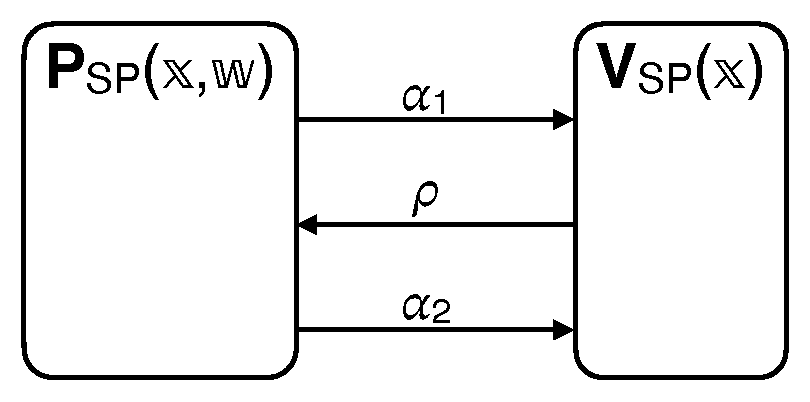
\includegraphics[width=0.5\textwidth]{\FigureFolder/sp-diagram}
\caption{Diagram of an SP.}
\label{figure:sp-diagram}
\end{figure}

The tuple $\SPSymbol=\SPSystem$ is a SP for a relation $\Relation$ with \emph{(perfect) completeness} and \emph{soundness error $\SPSoundnessError$} if it satisfies the two properties stated below.\footnote{This slightly deviates from the cryptography literature, where sigma protocols are assumed to satisfy stronger notions of security than the ones in this chapter. Specifically, in the cryptography literature, a sigma protocol satisfies \emph{special soundness} (rather than merely standard soundness as in this chapter) and special honest-verifier zero-knowledge (rather than merely honest-verifier zero-knowledge as in this chapter). This choice is for consistency with other parts of the book, and we separately consider strong soundness notions like special soundness (in \Cref{chapter:special-soundness}).}

\begin{definition}
\label{definition:sp-completeness}
$\SPSymbol=\SPSystem$ for a relation $\Relation$ has \defemph{perfect completeness} if for every $(\Instance,\Witness) \in \Relation$,
\begin{equation*}
\Pr\left[
\SPVerifier(\Instance,\SPCommitment,\SPChallenge,\SPResponse)=1
\GivenExperiment
\StateExperiment{
(\SPCommitment,\AuxiliaryState) \gets \SPProver(\Instance,\Witness) \\
\SPChallenge \gets \Bits^{\SPRandomnessComplexity} \\
\SPResponse \gets \SPProver(\AuxiliaryState,\SPChallenge)
}
\right]
=1
\enspace.
\end{equation*}
\end{definition}

\begin{definition}
\label{definition:sp-soundness}
$\SPSymbol=\SPSystem$ for a relation $\Relation$ has \defemph{soundness error $\SPSoundnessError$} if for every $\Instance \notin \GetLanguage{\Relation}$ and malicious SP prover $\SPMaliciousProver$,
\begin{equation*}
\Pr\left[
\SPVerifier(\Instance,\SPCommitment,\SPChallenge,\SPResponse)=1
\GivenExperiment
\StateExperiment{
(\SPCommitment,\AuxiliaryState) \gets \SPMaliciousProver \\
\SPChallenge \gets \Bits^{\SPRandomnessComplexity} \\
\SPResponse \gets \SPMaliciousProver(\AuxiliaryState,\SPChallenge)
}
\right]
\leq
\SPSoundnessError(\Instance)
\enspace.
\end{equation*}
We additionally define $\SPSoundnessError(\InstanceSize) \DefineEqual \MaxSoundness{\SPSoundnessError(\Instance)}$.
\end{definition}

A malicious SP prover $\SPMaliciousProver$ is all-powerful, so the soundness condition in \Cref{definition:sp-soundness} is equivalent to the following:
\begin{equation}
\label{equation:sp-alternative-soundness}
\forall\,\Instance \notin \GetLanguage{\Relation}\;\;
\forall\,\SPCommitment \in \Bits^{\SPPToVComplexity_{1}}\;
\Pr_{\SPChallenge \in \Bits^{\SPRandomnessComplexity}}
\left[
\exists\, \SPResponse \in \Bits^{\SPPToVComplexity_{2}} :
\SPVerifier(\Instance,\SPCommitment,\SPChallenge,\SPResponse)=1
\right]
\leq \SPSoundnessError(\Instance)
\enspace.
\end{equation}

\parhead{Knowledge soundness}
The soundness notion (\Cref{definition:sp-soundness}) can be strengthened to a knowledge soundness notion, which informally means that whenever an SP prover convinces the SP verifier then an efficient extractor finds a witness, up to some error. In more detail, we require the existence of a probabilistic algorithm $\SPExtractor$ that works as follows. Fix any instance $\Instance$ and SP prover $\SPMaliciousProver$. The SP prover $\SPMaliciousProver$ and SP verifier $\SPVerifier$ (on input $\Instance$) interact; denote by $(\SPCommitment,\SPChallenge,\SPResponse)$ the transcript of this interaction and by $b$ the decision bit of the SP verifier $\SPVerifier$. The knowledge extractor $\SPExtractor$ is tasked to find a witness $\Witness$ when given as input the instance $\Instance$, the interaction transcript $(\SPCommitment,\SPChallenge,\SPResponse)$, and black-box access to the SP prover $\SPMaliciousProver$. This means that the knowledge extractor $\SPExtractor$ is \emph{rewinding}: it can re-run the SP prover $\SPMaliciousProver$ multiple times, possibly with correlated inputs. The knowledge soundness error is an upper bound on the probability that $b=1$ ($\SPMaliciousProver$ convinces $\SPVerifier$) and $(\Instance,\Witness) \notin \Relation$ ($\SPExtractor$ does not find a witness). In general, the knowledge soundness error may be a function of the failure probability of $\SPMaliciousProver$, which we define below.

\begin{definition}
\label{definition:sp-failure-probability}
Let $\SPSymbol=\SPSystem$ be an SP. A deterministic SP prover $\SPMaliciousProver$ has \defemph{failure probability $\ProverFailureProbability{\SPMaliciousProver}$} if for every instance $\Instance$:
\begin{equation*}
\Pr\left[
\SPVerifier(\Instance,\SPCommitment,\SPChallenge,\SPResponse)=0
\GivenExperiment
\StateExperiment{
(\SPCommitment,\AuxiliaryState) \gets \SPMaliciousProver \\
\SPChallenge \gets \Bits^{\SPRandomnessComplexity} \\
\SPResponse \gets \SPMaliciousProver(\AuxiliaryState,\SPChallenge)
}
\right]
\leq \ProverFailureProbability{\SPMaliciousProver}(\Instance)
\enspace.
\end{equation*}
\end{definition}

\begin{definition}
\label{definition:sp-knowledge-soundness}
$\SPSymbol=\SPSystem$ for a relation $\Relation$ has \defemph{rewinding knowledge soundness error $\SPKnowledgeError$ with extraction time $\SPKnowledgeTime$} if there exists a probabilistic algorithm $\SPExtractor$ (the \emph{extractor}) such that for every instance $\Instance$ and deterministic SP prover $\SPMaliciousProver$ running in time $\ProverRunningTime{\SPMaliciousProver}$ the following holds:
\begin{equation*}
\Pr\left[
\begin{array}{l}
(\Instance,\Witness) \notin \Relation \\
\land\;\SPVerifier(\Instance,\SPCommitment,\SPChallenge,\SPResponse)=1
\end{array}
\GivenExperiment
\StateExperiment{
(\SPCommitment,\AuxiliaryState) \gets \SPMaliciousProver \\
\SPChallenge \gets \Bits^{\SPRandomnessComplexity} \\
\SPResponse \gets \SPMaliciousProver(\AuxiliaryState,\SPChallenge) \\
\Witness \gets \SPExtractor(\Instance,\SPCommitment,\SPChallenge,\SPResponse,\BlackBox{\SPMaliciousProver})
}
\right]
\leq
\SPKnowledgeError(\Instance,\ProverFailureProbability{\SPMaliciousProver}(\Instance))
\enspace.
\end{equation*}
Moreover, $\SPExtractor(\Instance,\SPCommitment,\SPChallenge,\SPResponse,\BlackBox{\SPMaliciousProver})$ runs in expected time $\SPKnowledgeTime(\Instance,\ProverFailureProbability{\SPMaliciousProver}(\Instance),\ProverRunningTime{\SPMaliciousProver}(\Instance))$ (over the given inputs and internal randomness). We additionally define
\begin{align*}
\SPKnowledgeError(\InstanceSize,\ProverFailureProbability{\SPMaliciousProver}) &\DefineEqual \MaxKnowledge{\SPKnowledgeError(\Instance,\ProverFailureProbability{\SPMaliciousProver}(\Instance))}
\enspace,\quad\text{and} \\
\SPKnowledgeTime(\InstanceSize,\ProverFailureProbability{\SPMaliciousProver},\ProverRunningTime{\SPMaliciousProver}) &\DefineEqual \MaxKnowledge{\SPKnowledgeTime(\Instance,\ProverFailureProbability{\SPMaliciousProver}(\Instance),\ProverRunningTime{\SPMaliciousProver}(\Instance))}
\enspace.
\end{align*}
\end{definition}

If $\SPSymbol=\SPSystem$ has knowledge soundness error $\SPKnowledgeError$ (with any extraction time $\SPKnowledgeTime$) then it has soundness error $\SPSoundnessError$ such that $\SPSoundnessError(\Instance) \leq  \min_{\ProverFailureProbability{} \in [0,1]} \SPKnowledgeError(\Instance,\ProverFailureProbability{})$: if $\Instance \notin \GetLanguage{\Relation}$ then the extractor cannot output a witness $\Witness$ such that $(\Instance,\Witness) \in \Relation$ (as none exists), in which case the event bounded by the knowledge soundness condition equals the event bounded by the soundness condition.

A notable special case of \Cref{definition:sp-knowledge-soundness} is \emph{straightline extraction}: $\SPExtractor$ is a polynomial-time deterministic algorithm that receives as input the instance $\Instance$ and SP prover messages $(\SPCommitment,\SPResponse)$ (but not the SP verifier challenge $\SPChallenge$ or access to $\SPMaliciousProver$).

\parhead{Zero knowledge}
An SP is \emph{zero knowledge} if the SP prover, when interacting with the SP verifier, reveals no information beyond the fact that the proved statement is true. If the SP verifier is allowed to behave arbitrarily, then the property is called \emph{malicious-verifier} zero knowledge; otherwise, if the SP verifier must follow the honest strategy, then the property is called \emph{honest-verifier} zero knowledge. This latter (and weaker) property suffices for the applications that we consider, and so our definitions focus on that property only. The formal definition consists of two steps:
\begin{inparaenum}[(a)]
  \item we formalize the \emph{view} of the SP verifier, which is all the information that the SP verifier learns by interacting with the SP prover;
  \item we say that the interactive proof is zero knowledge if the view of the SP verifier can be (approximately) simulated by a polynomial-time probabilistic algorithm, known as the \emph{simulator}.
\end{inparaenum}
The intuition here is that anything that is computable efficiently with randomness is \DoQuote{for free}, and so does not count as revealed knowledge. Crucially, the property is only required to hold for true statements, and the simulator is only given as input the statement (but not any \DoQuote{help} such as a witness, which may be hard to compute).

\begin{definition}
\label{definition:sp-view}
The SP verifier's \defemph{view} in $\SPSymbol=\SPSystem$ on the instance-witness pair $(\Instance,\Witness)$, denoted $\SPView{\SPProver}{\SPVerifier}{\Instance}{\Witness}$, is the random variable $\SPSampledView$ where:
\begin{itemize}[nolistsep]
  \item $(\SPCommitment,\AuxiliaryState) \gets \SPProver(\Instance,\Witness)$;
  \item $\SPChallenge$ is a random choice of randomness for the SP verifier $\SPVerifier$; and
  \item $\SPResponse \gets \SPProver(\AuxiliaryState,\SPChallenge)$.
\end{itemize}
Note that the honest SP prover $\SPProver(\Instance,\Witness)$ may use its own private randomness (and is not part of the SP verifier's view).
\end{definition}

\begin{definition}
\label{definition:sp-hvzk}
$\SPSymbol=\SPSystem$ for a relation $\Relation$ has \defemph{honest-verifier zero-knowledge error $\SPZKError$} if there exists a polynomial-time probabilistic algorithm $\SPSimulator$ such that for every instance-witness pair $(\Instance,\Witness) \in \Relation$ the following random variables are $\SPZKError(\Instance)$-close in statistical distance:
\begin{equation*}
\SPView{\SPProver}{\SPVerifier}{\Instance}{\Witness}
\TextAndInMath
\SPSimulator(\Instance)
\enspace.
\end{equation*}
We additionally define $\SPZKError(\InstanceSize) \DefineEqual \MaxZK{\SPZKError(\Instance)}$.
\end{definition}


\begin{remark}[comparison with prior definitions of knowledge soundness]
\label{remark:comparison-with-prior-knowledge-soundness}
\Cref{definition:sp-knowledge-soundness} strengthens definitions of rewinding knowledge soundness commonly used in the literature. \Cref{definition:sp-knowledge-soundness} considers a single probability experiment in which the prover is run and subsequently the extractor receives as input the transcript of interaction and black-box access to the prover. This is in contrast to traditional definitions of rewinding knowledge soundness, which consider two probability experiments, one for the prover (considering the prover's success probability) and one for the extractor (considering the extractor's success probability).

\Cref{definition:sp-knowledge-soundness} facilitates achieving \emph{adaptive} rewinding knowledge soundness for corresponding non-interactive arguments (according to \Cref{definition:adaptive-rewinding-knowledge-soundness}, and its equivalent \Cref{definition:adaptive-rewinding-knowledge-soundness-verifier-trace}). We use the same \DoQuote{single-experiment format} as \Cref{definition:sp-knowledge-soundness} for all other notions of rewinding knowledge soundness in this book: \Cref{definition:ip-knowledge-soundness} for IPs and \Cref{definition:iop-knowledge-soundness} for IOPs; and also for all corresponding state-restoration strengthenings in \Cref{definition:sp-state-restoration-knowledge,definition:ip-state-restoration-knowledge,definition:iop-state-restoration-knowledge}.

We show how \Cref{definition:sp-knowledge-soundness} implies a common definition of rewinding knowledge soundness (there are others in the literature, also implied similarly).
\begin{center}
\begin{minipage}{0.9\textwidth}
There exists an extractor $\SPExtractor'$ such that for every adversary $\SPMaliciousProver$:
\begin{align*}
&\Pr\left[
(\Instance,\Witness) \in \Relation
\GivenExperiment
\StateExperiment{
  \Witness \gets \SPExtractor'(\Instance,\BlackBox{\SPMaliciousProver})
}
\right]
\\ & \geq
\Pr\left[
  \SPVerifier(\Instance,\SPCommitment,\SPChallenge,\SPResponse)=1
\GivenExperiment
\StateExperiment{
  (\SPCommitment,\AuxiliaryState) \gets \SPMaliciousProver \\
  \SPChallenge \gets \Bits^{\SPRandomnessComplexity} \\
  \SPResponse \gets \SPMaliciousProver(\AuxiliaryState,\SPChallenge)
}
\right]
-
\SPKnowledgeError(\Instance,\ProverFailureProbability{\SPMaliciousProver}(\Instance))
\enspace.
\end{align*}
\end{minipage}
\end{center}
We show that if $\SPSymbol=\SPSystem$ satisfies \Cref{definition:sp-knowledge-soundness} with an extractor $\SPExtractor$ then $\SPSymbol=\SPSystem$ satisfies the above definition with the extractor $\SPExtractor'$ defined below.
\begin{itemize}[noitemsep]
\item[] $\SPExtractor'(\Instance,\BlackBox{\SPMaliciousProver})$:
\begin{enumerate}[nolistsep]
  \item Compute $(\SPCommitment,\AuxiliaryState) \gets \SPMaliciousProver$.
  \item Sample $\SPChallenge \gets \Bits^{\SPRandomnessComplexity}$.
  \item Compute $\SPResponse \gets \SPMaliciousProver(\AuxiliaryState,\SPChallenge)$.
  \item Compute $\Witness \gets \SPExtractor(\Instance,\SPCommitment,\SPChallenge,\SPResponse,\BlackBox{\SPMaliciousProver})$.
  \item Output $\Witness$.
\end{enumerate}
\end{itemize}
We get that
\begin{align*}
&\Pr\left[
(\Instance,\Witness) \in \Relation
\GivenExperiment
\StateExperiment{
  \Witness \gets \SPExtractor'(\Instance,\BlackBox{\SPMaliciousProver})
}
\right]
\\ & =
\Pr\left[
(\Instance,\Witness) \in \Relation
\GivenExperiment
\StateExperiment{
  (\SPCommitment,\AuxiliaryState) \gets \SPMaliciousProver \\
  \SPChallenge \gets \Bits^{\SPRandomnessComplexity} \\
  \SPResponse \gets \SPMaliciousProver(\AuxiliaryState,\SPChallenge) \\
  \Witness \gets \SPExtractor(\Instance,\SPCommitment,\SPChallenge,\SPResponse,\BlackBox{\SPMaliciousProver})
}
\right] \EquationComment{by definition of $\SPExtractor'$}
\\ & \geq
\Pr\left[
\begin{array}{l}
  (\Instance,\Witness) \in \Relation \\
  \land\;\SPVerifier(\Instance,\SPCommitment,\SPChallenge,\SPResponse)=1
\end{array}
\GivenExperiment
\StateExperiment{
  (\SPCommitment,\AuxiliaryState) \gets \SPMaliciousProver \\
  \SPChallenge \gets \Bits^{\SPRandomnessComplexity} \\
  \SPResponse \gets \SPMaliciousProver(\AuxiliaryState,\SPChallenge) \\
  \Witness \gets \SPExtractor(\Instance,\SPCommitment,\SPChallenge,\SPResponse,\BlackBox{\SPMaliciousProver})
}
\right]
\\ & =
\Pr\left[
\SPVerifier(\Instance,\SPCommitment,\SPChallenge,\SPResponse)=1
\GivenExperiment
\StateExperiment{
  (\SPCommitment,\AuxiliaryState) \gets \SPMaliciousProver \\
  \SPChallenge \gets \Bits^{\SPRandomnessComplexity} \\
  \SPResponse \gets \SPMaliciousProver(\AuxiliaryState,\SPChallenge) \\
  \Witness \gets \SPExtractor(\Instance,\SPCommitment,\SPChallenge,\SPResponse,\BlackBox{\SPMaliciousProver})
}
\right]
\\ & \; \; -
\Pr\left[
\begin{array}{l}
  (\Instance,\Witness) \notin \Relation \\
  \land\;\SPVerifier(\Instance,\SPCommitment,\SPChallenge,\SPResponse)=1
\end{array}
\GivenExperiment
\StateExperiment{
  (\SPCommitment,\AuxiliaryState) \gets \SPMaliciousProver \\
  \SPChallenge \gets \Bits^{\SPRandomnessComplexity} \\
  \SPResponse \gets \SPMaliciousProver(\AuxiliaryState,\SPChallenge) \\
  \Witness \gets \SPExtractor(\Instance,\SPCommitment,\SPChallenge,\SPResponse,\BlackBox{\SPMaliciousProver})
}
\right]
\\ & \geq
\Pr\left[
  \SPVerifier(\Instance,\SPCommitment,\SPChallenge,\SPResponse)=1
\GivenExperiment
\StateExperiment{
  (\SPCommitment,\AuxiliaryState) \gets \SPMaliciousProver \\
  \SPChallenge \gets \Bits^{\SPRandomnessComplexity} \\
  \SPResponse \gets \SPMaliciousProver(\AuxiliaryState,\SPChallenge)
}
\right]
-
\SPKnowledgeError(\Instance,\ProverFailureProbability{\SPMaliciousProver}(\Instance))
\enspace.
\end{align*}
\end{remark}


%%%%%%%%%%%%%%%%%%%%%%%%%%%%%%%%%%%%%%%%%%%%%%%%%%%%%%%%%%%%%%%%%%%%%%%%%%%%%%%
%%%%%%%%%%%%%%%%%%%%%%%%%%%%%%%%%%%%%%%%%%%%%%%%%%%%%%%%%%%%%%%%%%%%%%%%%%%%%%%
%%%%%%%%%%%%%%%%%%%%%%%%%%%%%%%%%%%%%%%%%%%%%%%%%%%%%%%%%%%%%%%%%%%%%%%%%%%%%%%
%%%%%%%%%%%%%%%%%%%%%%%%%%%%%%%%%%%%%%%%%%%%%%%%%%%%%%%%%%%%%%%%%%%%%%%%%%%%%%%
\chapter{Warmup: non-adaptive security}
\label{chapter:warmup-narg-from-sp-nonadaptive-security}

We describe how to transform any sigma protocol (SP) into a non-interactive argument that has \emph{non}-adaptive security, via a simple warmup construction.

\parhead{Organization}
In \Cref{section:warmup-narg-from-sp-construction} we describe the construction. In \Cref{section:warmup-narg-from-sp-lower-bound} we show a lower bound on the non-adaptive soundness error. In \Cref{section:warmup-narg-from-sp-nonadaptive-soundness} we show non-adaptive soundness. In \Cref{section:warmup-narg-from-sp-nonadaptive-knowledge-soundness} we show non-adaptive knowledge soundness. In \Cref{section:warmup-narg-from-sp-nonadaptive-zk} we show non-adaptive zero knowledge. In \Cref{section:warmup-narg-from-sp-no-adaptive-security} we explain why the construction does \emph{not} have adaptive security.



%%%%%%%%%%%%%%%%%%%%%%%%%%%%%%%%%%%%%%%%%%%%%%%%%%%%%%%%%%%%%%%%%%%%%%%%%%%%%%%
%%%%%%%%%%%%%%%%%%%%%%%%%%%%%%%%%%%%%%%%%%%%%%%%%%%%%%%%%%%%%%%%%%%%%%%%%%%%%%%
%%%%%%%%%%%%%%%%%%%%%%%%%%%%%%%%%%%%%%%%%%%%%%%%%%%%%%%%%%%%%%%%%%%%%%%%%%%%%%%
\section{Construction}
\label{section:warmup-narg-from-sp-construction}

The main idea is that the argument prover can use the random oracle to produce the SP verifier challenge in a way that is independent of the SP commitment, and subsequently send an argument string that contains the SP commitment and SP response.

In more detail, the SP verifier participates in the interaction only by sending its challenge $\SPChallenge$ after receiving the SP prover commitment $\SPCommitment$. Hence, the argument prover can query the random oracle $\ROFunction$ at $\SPCommitment$ to obtain $\SPChallenge \DefineEqual \ROFunction(\SPCommitment)$ as a challenge. By definition of the random oracle, the answer $\ROFunction(\SPCommitment)$ is uniformly random. The argument prover can then compute its response $\SPResponse$ based on $\ROFunction(\SPCommitment)$, and send the argument string $\ARGString \DefineEqual (\SPCommitment,\SPResponse)$. The argument verifier can then run the SP verifier decision predicate on the commitment $\SPCommitment$, challenge $\ROFunction(\SPCommitment)$, and response $\SPResponse$.

The output size of the random oracle and the size of an SP challenge must equal. An SP challenge $\SPChallenge$ consists of $\SPRandomnessComplexity$ bits, so the random oracle $\ROFunction$ is sampled from $\RODistribution{\SPRandomnessComplexity}$.



\begin{construction}
\label{construction:warmup-narg-from-sp}
Let $\SPSymbol=\SPSystem$ be an SP. Consider the non-interactive argument $\NARGSymbol=\ARGSystem$ constructed as follows. The argument prover $\ARGProver$ receives as input an instance $\Instance$ and witness $\Witness$, and the argument verifier $\ARGVerifier$ receives as input the instance $\Instance$ and an argument string $\ARGString$. Both receive query access to a random oracle $\ROFunction \in \RODistribution{\SPRandomnessComplexity}$; this implies that the oracle configuration $\ARGOracles$ is defined as $\ARGOracles(\SecurityParameter,\InstanceSize) \DefineEqual \SPRandomnessComplexity$ (see \Cref{definition:narg-oracle-configuration}).
\begin{itemize}
  \item $\ARGProver^{\ROFunction}(\Instance,\Witness)$:
  \begin{enumerate}[nolistsep]
    \item Run the SP prover to obtain the first message and auxiliary state: $(\SPCommitment,\AuxiliaryState) \gets \SPProver(\Instance,\Witness)$.
    \item \label{step:warmup-fs-for-sp-challenge-derivation}
    Derive the SP verifier challenge as $\SPChallenge \DefineEqual \ROFunction(\SPCommitment)$.
    \item Run the SP prover to obtain the second message: $\SPResponse \gets \SPProver(\AuxiliaryState,\SPChallenge)$.
    \item Output the argument string $\ARGString \DefineEqual (\SPCommitment,\SPResponse)$.
  \end{enumerate}
  \item $\ARGVerifier^{\ROFunction}(\Instance,\ARGString)$:
  \begin{enumerate}[nolistsep]
    \item Parse the argument string $\ARGString$ as a commitment-response pair $(\SPCommitment,\SPResponse)$.
    \item Derive the SP verifier challenge $\SPChallenge$ as in \Cref{step:warmup-fs-for-sp-challenge-derivation} of the argument prover $\ARGProver$.
    \item Check that the SP verifier accepts: $\SPVerifier(\Instance,\SPCommitment,\SPChallenge,\SPResponse)=1$.
  \end{enumerate}
\end{itemize}
\end{construction}

\begin{figure}[htp!]
\centering
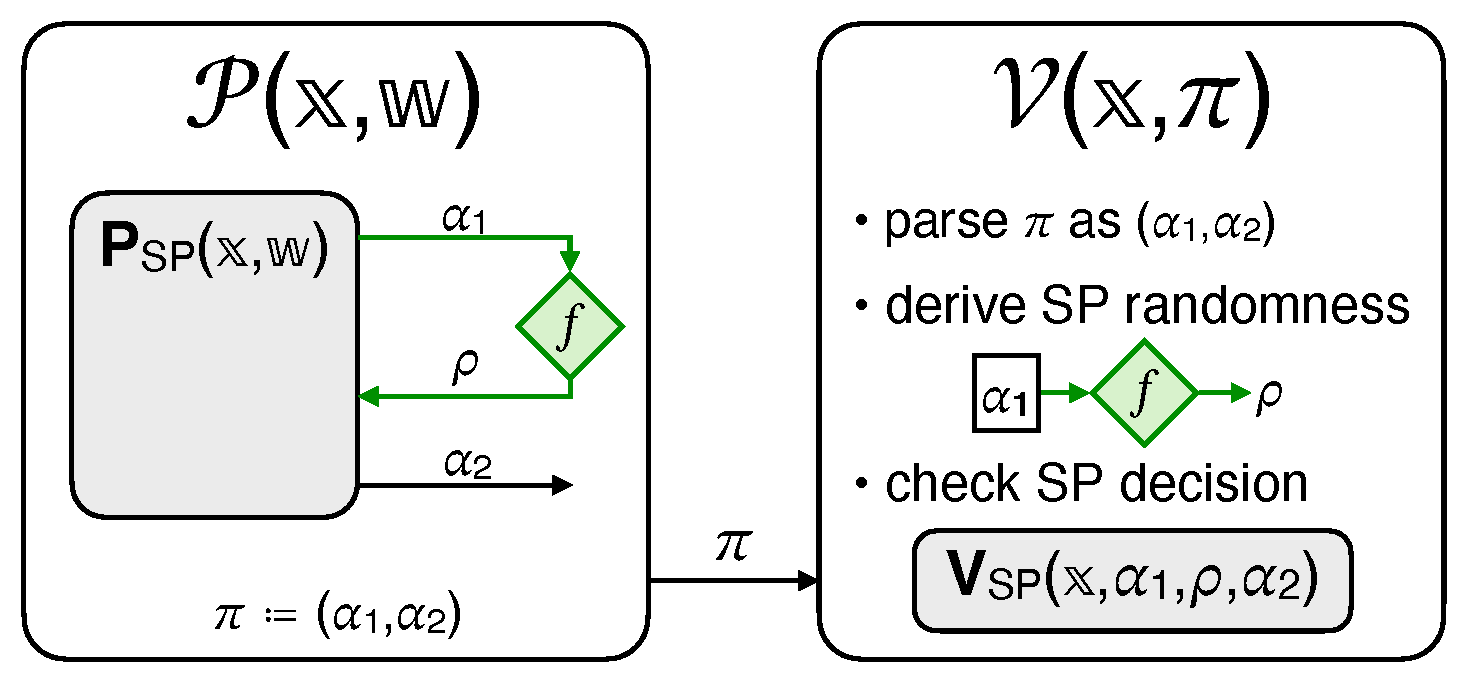
\includegraphics[width=0.65\textwidth]{\FigureFolder/warmup-fs-sp-diagram}
\caption{Diagram of \Cref{construction:warmup-narg-from-sp}.}
\label{figure:warmup-narg-from-sp}
\end{figure}

%%%%%%%%%%%%%%%%%%%%%%%%%%%%%%%%%%%%%%%%%%%%%%%%%%%%%%%%%%%%%%%%%%%%%%%%%%%%%%%
%%%%%%%%%%%%%%%%%%%%%%%%%%%%%%%%%%%%%%%%%%%%%%%%%%%%%%%%%%%%%%%%%%%%%%%%%%%%%%%
%%%%%%%%%%%%%%%%%%%%%%%%%%%%%%%%%%%%%%%%%%%%%%%%%%%%%%%%%%%%%%%%%%%%%%%%%%%%%%%
\section{Lower bound on the non-adaptive soundness error}
\label{section:warmup-narg-from-sp-lower-bound}

We describe a malicious argument prover that \DoQuote{attacks} \Cref{construction:warmup-narg-from-sp}, thereby establishing a lower-bound on the non-adaptive soundness error. This provides the basic intuition for what non-adaptive soundness error we should expect of this construction.

Informally, while a malicious SP prover has only a \emph{single} chance to convince the SP verifier, a malicious argument prover for \Cref{construction:warmup-narg-from-sp} has \emph{multiple} chances to convince the SP verifier that underlies the argument verifier. Intuitively, this means that the soundness error of the non-interactive argument is \emph{not} equal to the soundness error of the SP (not even up to a small additive error). Instead, in general, the transformation incurs a multiplicative factor in soundness error that is proportional to the number of chances to convince the underlying SP verifier.

In more detail, we formalize the above intuition via an attack that works when transforming SPs that satisfy a certain property.\footnote{We cannot expect an attack that works for \emph{every} SP. For example, if the underlying SP has soundness error $0$ then so does the non-interactive argument (because, in the soundness case, there is no way to convince the underlying SP verifier regardless of the number of attempts).} Consider an SP for a given relation $\Relation$ that satisfies the following mild requirement (satisfied by natural SPs):
\begin{equation}
\label{equation:sp-attack-property}
\exists\,\Instance \notin \GetLanguage{\Relation},\;
\forall\,\SPCommitment \in \Bits^{\SPPToVComplexity_{1}}\;
\Pr\left[
\begin{array}{l}
\exists\, \SPResponse \in \Bits^{\SPPToVComplexity_{2}} \text{ s.t.} \\
\SPVerifier(\Instance,\SPCommitment,\SPChallenge,\SPResponse)=1
\end{array}
\GivenExperiment
\StateExperiment{
\SPChallenge \gets \Bits^{\SPRandomnessComplexity}
}
\right]
=
\SPSoundnessError(\Instance)
\enspace.
\end{equation}
For a given query bound $\ROQueryBound \in \Naturals$, consider the $\ROQueryBound$-query argument prover $\Malicious{\ARGProver}$ defined as follows:
\begin{enumerate}[noitemsep]
  \item For up to $\ROQueryBound$ times:
  \begin{enumerate}[nolistsep]
    \item Choose any SP prover first message $\SPCommitment \in \Bits^{\SPPToVComplexity_{1}}$ that was not previously chosen.
    \item Query the random oracle to compute the SP verifier challenge $\SPChallenge \DefineEqual \ROFunction(\SPCommitment)$.
    \item If there exists $\SPResponse \in \Bits^{\SPPToVComplexity_{2}}$ such that $\SPVerifier(\Instance,\SPCommitment,\SPChallenge,\SPResponse)=1$ then output $\ARGString \DefineEqual (\SPCommitment,\SPResponse)$.
  \end{enumerate}
  \item Output $\ARGString \DefineEqual \bot$.
\end{enumerate}

\begin{lemma}
\label{lemma:attack-against-warmup-narg-from-sp}
Let $\SPSymbol=\SPSystem$ be an SP for a relation $\Relation$ that satisfies \Cref{equation:sp-attack-property}. Then $\NARGSymbol=\ARGSystem$ defined in \Cref{construction:warmup-narg-from-sp} is a non-interactive argument for $\Relation$ with non-adaptive soundness error $\ARGSoundnessError$ (see \Cref{definition:narg-nonadaptive-soundness-with-cnf}) such that there exists $\Instance \notin \GetLanguage{\Relation}$ such that for every security parameter $\SecurityParameter \in \Naturals$ and query bound $\ROQueryBound \in \Naturals$,
\begin{equation*}
\ARGSoundnessError(\SecurityParameter,\ROQueryBound,\Instance)
\geq
\ROQueryBound \cdot \SPSoundnessError(\Instance) -
\binom{\ROQueryBound}{2} \cdot \SPSoundnessError(\Instance)^2
\enspace.
\end{equation*}
In particular, if $\ROQueryBound \cdot \SPSoundnessError(\Instance) \leq 1$ then the lower bound is at least $\frac{\ROQueryBound}{2} \cdot \SPSoundnessError(\Instance)$.
\end{lemma}

\begin{proof}
Fix an instance $\Instance \notin \GetLanguage{\Relation}$ that satisfies \Cref{equation:sp-attack-property}. We use the inclusion-exclusion principle (\Cref{lemma:inclusion-exclusion-2}) to lower bound the winning probability of $\Malicious{\ARGProver}$. For every $i \in [\ROQueryBound]$, let $\SPCommitmentIndexed{i} \in \Bits^{\SPPToVComplexity_{1}}$ be the $i$-th query of $\Malicious{\ARGProver}$ and let $\RandomVariableX_{i}$ be the indicator random variable for the event that there exists $\SPResponse \in \Bits^{\SPPToVComplexity_{2}}$ such that $\SPVerifier(\Instance,\SPCommitmentIndexed{i},\ROFunction(\SPCommitmentIndexed{i}),\SPResponse)=1$. The random variables $(\RandomVariableX_{i})_{i \in [\ROQueryBound]}$ are independent. From \Cref{equation:sp-attack-property}, we know that $\Pr[\RandomVariableX_{i}=1] = \SPSoundnessError(\Instance)$. Therefore we get that
\begin{align*}
&\Pr\left[
\ARGVerifier^{\ROFunction}(\Instance,\ARGString)=1
\GivenExperiment
\StateExperiment{
\ROFunction \gets \RODistribution{\SPRandomnessComplexity} \\
\ARGString \gets \Malicious{\ARGProver}^{\ROFunction}
}
\right] \\
& = \Pr\left[
\SPVerifier(\Instance,\SPCommitment,\ROFunction(\SPCommitment),\SPResponse)=1
\GivenExperiment
\StateExperiment{
\ROFunction \gets \RODistribution{\SPRandomnessComplexity} \\
(\SPCommitment,\SPResponse) \gets \Malicious{\ARGProver}^{\ROFunction}
}
\right] \EquationComment{by definition of $\ARGVerifier$}
\\ & =
\Pr[\exists\, i \in [\ROQueryBound] :  \RandomVariableX_{i}=1] \EquationComment{by definition of $\Malicious{\ARGProver}$}
\\ & \geq
\sum_{i \in [\ROQueryBound]}\Pr[\RandomVariableX_{i}=1] - \sum_{\substack{i,j \in [\ROQueryBound] \\ \text{with } i \neq j}}\Pr[\RandomVariableX_{i} \cdot \RandomVariableX_{j}=1] \EquationComment{by \Cref{lemma:inclusion-exclusion-2}}
\\ & =
\sum_{i \in [\ROQueryBound]}\Pr[\RandomVariableX_{i}=1] - \sum_{\substack{i,j \in [\ROQueryBound] \\ \text{with } i \neq j}}\Pr[\RandomVariableX_{i}=1] \cdot \Pr[\RandomVariableX_{j}=1] \EquationComment{by independence}
\\ & =
\ROQueryBound \cdot \SPSoundnessError(\Instance) -
\binom{\ROQueryBound}{2} \cdot \SPSoundnessError(\Instance)^2
\enspace.
\end{align*}
\end{proof}

We conclude that \Cref{construction:warmup-narg-from-sp} is \emph{not} sound if the underlying SP does not have small enough soundness error. Next we wish to understand the converse: is \Cref{construction:warmup-narg-from-sp} sound if the underlying SP has small enough soundness error?

\begin{remark}
\label{remark:attack-against-narg-from-sp}
The malicious argument prover $\Malicious{\ARGProver}$ described above attempts to convince the SP verifier with $\ROQueryBound$ queries, and if it fails it outputs the empty argument string $\ARGString \DefineEqual \bot$. A minor improvement is to \emph{not} output the empty argument string: if all $\ROQueryBound$ queries fail then $\Malicious{\ARGProver}$ outputs $\ARGString \DefineEqual (\SPCommitment,\SPResponse)$ for any first message $\SPCommitment$ not queried so far and the best response $\SPResponse$ for $\SPCommitment$. For specific SPs, this is tantamount to $\Malicious{\ARGProver}$ having an additional query due to the chance that a tuple $(\SPCommitment,\SPResponse)$ sampled this way convinces the SP verifier. This explains why, in the soundness analysis in \Cref{section:warmup-narg-from-sp-nonadaptive-soundness}, we obtain the multiplicative factor $\ROQueryBound+1$ in the soundness error, rather than $\ROQueryBound$.
\end{remark}

%%%%%%%%%%%%%%%%%%%%%%%%%%%%%%%%%%%%%%%%%%%%%%%%%%%%%%%%%%%%%%%%%%%%%%%%%%%%%%%
%%%%%%%%%%%%%%%%%%%%%%%%%%%%%%%%%%%%%%%%%%%%%%%%%%%%%%%%%%%%%%%%%%%%%%%%%%%%%%%
%%%%%%%%%%%%%%%%%%%%%%%%%%%%%%%%%%%%%%%%%%%%%%%%%%%%%%%%%%%%%%%%%%%%%%%%%%%%%%%
\section{Non-adaptive soundness}
\label{section:warmup-narg-from-sp-nonadaptive-soundness}

We prove that \Cref{construction:warmup-narg-from-sp} has non-adaptive soundness error $\ARGSoundnessError(\SecurityParameter,\ROQueryBound,\Instance) \leq (\ROQueryBound+1) \cdot \SPSoundnessError(\Instance)$. This shows that \Cref{construction:warmup-narg-from-sp} is non-adaptively sound if the underlying SP has a small enough soundness error and that the attack in \Cref{section:warmup-narg-from-sp-lower-bound} is essentially optimal. Later in \Cref{section:fs-lack-of-adaptive-soundness} we explain why \Cref{construction:warmup-narg-from-sp} does not achieve adaptive soundness.

We provide two security analyses.
\begin{itemize}
  \item In \Cref{section:warmup-narg-from-sp-inefficient-reduction} we provide an analysis that directly upper bounds the non-adaptive soundness error of the non-interactive argument by invoking the upper bound on the soundness error of the underlying SP.
  \item In \Cref{section:warmup-narg-from-sp-efficient-reduction} we provide an alternative analysis: we prove that every malicious argument prover can be \emph{efficiently} transformed into a corresponding malicious SP prover with a multiplicative loss of $\ROQueryBound+1$ in convincing probability.
\end{itemize}
The alternative analysis shows the same upper bound for the non-adaptive soundness error but is a stronger statement: it provides an efficient method to translate strategies for convincing the argument verifier into strategies for convincing the SP verifier.

In the rest of this book, we always provide \emph{efficient security analyses} (efficient transformations of adversaries, analogous to that in \Cref{section:warmup-narg-from-sp-efficient-reduction}) because an efficient translation of adversarial strategies is useful in many settings. We give two examples.
\begin{itemize}
  \item An efficient translation of adversarial strategies is typically one of the steps to establishing knowledge soundness. In \Cref{section:warmup-narg-from-sp-nonadaptive-knowledge-soundness} we see how the efficient translation of adversarial strategies plays a role towards the knowledge soundness of \Cref{construction:warmup-narg-from-sp}.
  \item If the underlying SP were to satisfy only computational soundness due to the use of cryptographic assumptions (i.e., the SP is in fact a $3$-message interactive argument), proving soundness of \Cref{construction:warmup-narg-from-sp} would require constructing an efficient adversary for the interactive argument from the given adversary of the non-interactive argument.
\end{itemize}

%%%%%%%%%%%%%%%%%%%%%%%%%%%%%%%%%%%%%%%%%%%%%%%%%%%%%%%%%%%%%%%%%%%%%%%%%%%%%%%
%%%%%%%%%%%%%%%%%%%%%%%%%%%%%%%%%%%%%%%%%%%%%%%%%%%%%%%%%%%%%%%%%%%%%%%%%%%%%%%
\subsection{An inefficient security reduction}
\label{section:warmup-narg-from-sp-inefficient-reduction}

\begin{lemma}
\label{lemma:warmup-narg-from-sp-inefficient-reduction}
Let $\SPSymbol=\SPSystem$ be an SP for a relation $\Relation$ with soundness error $\SPSoundnessError$. Then $\NARGSymbol=\ARGSystem$ defined in \Cref{construction:warmup-narg-from-sp} is a non-interactive argument for $\Relation$ with non-adaptive soundness error $\ARGSoundnessError$ (see \Cref{definition:narg-adaptive-soundness-with-cnf}) such that for every instance $\Instance \notin \GetLanguage{\Relation}$,
\begin{equation*}
\ARGSoundnessError(\SecurityParameter,\ROQueryBound,\Instance)
\leq
(\ROQueryBound+1) \cdot \SPSoundnessError(\Instance)
\enspace.
\end{equation*}
\end{lemma}

\begin{proof}
Let $\Malicious{\ARGProver}$ be a $\ROQueryBound$-query malicious argument prover that outputs an argument string $\ARGString = (\SPCommitment,\SPResponse)$. We upper bound the probability that $\ARGVerifier^{\ROFunction}(\Instance,\ARGString)=1$.
\begin{itemize}

  \item \emph{Case 1: $\SPCommitment$ is a query in the trace.}
We argue that
\begin{equation*}
\Pr\left[
\begin{array}{l}
\SPVerifier(\Instance,\SPCommitment,\ROFunction(\SPCommitment),\SPResponse)=1 \\
\land\;\big(\SPCommitment,\ROFunction(\SPCommitment)\big) \in \ROTrace
\end{array}
\GivenExperiment
\StateExperiment{
\ROFunction \gets \RODistribution{\SPRandomnessComplexity} \\
\ROOutputAndTrace{\ROFunction}{\Malicious{\ARGProver}}{\ROTrace}{(\SPCommitment,\SPResponse)}
}
\right]
\leq
\ROQueryBound \cdot \SPSoundnessError(\Instance)
\enspace.
\end{equation*}
We upper bound the probability that there exists a query-answer pair $(\SPCommitment,\SPChallenge) \in \ROTrace$ and a response $\SPResponse \in \Bits^{\SPPToVComplexity_{2}}$ such that $\SPVerifier(\Instance,\SPCommitment,\SPChallenge,\SPResponse)=1$. The soundness of the SP (see \Cref{equation:sp-alternative-soundness}) gives that for every (distinct) query $\SPCommitment \in \Bits^{\SPPToVComplexity_{1}}$ it holds that
\begin{align*}
\Pr\left[
\begin{array}{l}
\exists\, \SPResponse \in \Bits^{\SPPToVComplexity_{2}} \text{ s.t.} \\
\SPVerifier(\Instance,\SPCommitment,\SPChallenge,\SPResponse)=1
\end{array}
\GivenExperiment
\StateExperiment{
\SPChallenge \in \Bits^{\SPRandomnessComplexity}
}
\right]
\leq
\SPSoundnessError(\Instance)
\enspace.
\end{align*}
Since $\Malicious{\ARGProver}$ performs at most $\ROQueryBound$ queries, we get that
\begin{align*}
\Pr\left[
\begin{array}{l}
 \SPVerifier(\Instance,\ROFunction(\SPCommitment),\SPChallenge,\SPResponse)=1 \\
 \land \; (\SPCommitment,\ROFunction(\SPCommitment)) \in \ROTrace
\end{array}
\GivenExperiment
\StateExperiment{
\ROFunction \gets \RODistribution{\SPRandomnessComplexity} \\
\ROOutputAndTrace{\ROFunction}{\Malicious{\ARGProver}}{\ROTrace}{(\SPCommitment,\SPResponse)}
}
\right]
\leq \ROQueryBound \cdot \SPSoundnessError(\Instance)
\enspace.
\end{align*}

  \item \emph{Case 2: $\SPCommitment$ is not a query in the trace.}
We argue that
\begin{equation*}
\Pr\left[
\begin{array}{l}
\SPVerifier(\Instance,\SPCommitment,\ROFunction(\SPCommitment),\SPResponse)=1 \\
\land\;\big(\SPCommitment,\ROFunction(\SPCommitment)\big) \notin \ROTrace
\end{array}
\GivenExperiment
\StateExperiment{
\ROFunction \gets \RODistribution{\SPRandomnessComplexity} \\
\ROOutputAndTrace{\ROFunction}{\Malicious{\ARGProver}}{\ROTrace}{(\SPCommitment,\SPResponse)}
}
\right]
\leq
\SPSoundnessError(\Instance)
\enspace.
\end{equation*}
Suppose that the malicious argument prover $\Malicious{\ARGProver}$ outputs $\SPCommitment$ that is not a query in the trace $\ROTrace$. Then, the response $\ROFunction(\SPCommitment)$ is random, and thus by the soundness of the SP, the probability that the SP verifier accepts in this case is at most $\SPSoundnessError(\Instance)$.

\end{itemize}
We conclude that
\begin{align*}
&\Pr\left[
\ARGVerifier^{\ROFunction}(\Instance,\ARGString)=1
\GivenExperiment
\StateExperiment{
\ROFunction \gets \RODistribution{\SPRandomnessComplexity} \\
\ARGString \gets \Malicious{\ARGProver}^{\ROFunction}
}
\right]
\\&=
\Pr\left[
\SPVerifier(\Instance,\SPCommitment,\ROFunction(\SPCommitment),\SPResponse)=1
\GivenExperiment
\StateExperiment{
\ROFunction \gets \RODistribution{\SPRandomnessComplexity} \\
(\SPCommitment,\SPResponse) \gets \Malicious{\ARGProver}^{\ROFunction}
}
\right]
\\&\leq
\ROQueryBound \cdot \SPSoundnessError(\Instance)
+
\SPSoundnessError(\Instance)
\\&=
(\ROQueryBound+1) \cdot \SPSoundnessError(\Instance)
\enspace.
\end{align*}
\end{proof}

%%%%%%%%%%%%%%%%%%%%%%%%%%%%%%%%%%%%%%%%%%%%%%%%%%%%%%%%%%%%%%%%%%%%%%%%%%%%%%%
%%%%%%%%%%%%%%%%%%%%%%%%%%%%%%%%%%%%%%%%%%%%%%%%%%%%%%%%%%%%%%%%%%%%%%%%%%%%%%%
\subsection{An efficient security reduction}
\label{section:warmup-narg-from-sp-efficient-reduction}

\begin{lemma}
\label{lemma:warmup-narg-from-sp-efficient-reduction}
Let $\SPSymbol=\SPSystem$ be an SP for a relation $\Relation$, and let $\NARGSymbol=\ARGSystem$ be the non-interactive argument defined in \Cref{construction:warmup-narg-from-sp}. There exists an SP prover $\SPMaliciousProver$ such that for every instance $\Instance$, query bound $\ROQueryBound \in \Naturals$, and malicious $\ROQueryBound$-query argument prover $\Malicious{\ARGProver}$,
\begin{align*}
&\Pr\left[
\ARGVerifier^{\ROFunction}(\Instance,\ARGString) = 1
\GivenExperiment
\StateExperiment{
\ROFunction \gets \RODistribution{\SPRandomnessComplexity} \\
\ARGString \gets \Malicious{\ARGProver}^{\ROFunction}
}
\right]
\\&\leq
(\ROQueryBound+1) \cdot
\Pr\left[
\SPVerifier(\Instance,\SPCommitment,\SPChallenge,\SPResponse)=1
\GivenExperiment
\StateExperiment{
(\SPCommitment, \AuxiliaryState) \gets \SPMaliciousProver(\BlackBox{\Malicious{\ARGProver}}) \\
\SPChallenge \gets \Bits^{\SPRandomnessComplexity} \\
\SPResponse \gets \SPMaliciousProver(\AuxiliaryState, \SPChallenge)
}
\right]
\enspace.
\end{align*}
Moreover, if the running time of $\Malicious{\ARGProver}$ is $\ARGTimeP$ then the running time of $\SPMaliciousProver$ is $\ARGTimeP + O(\SPRandomnessComplexity \cdot \ROQueryBound)$.
\end{lemma}

\begin{construction}
\label{construction:fs-for-sp-efficient-reduction}
The SP prover $\SPMaliciousProver$ is parametrized by the query bound $\ROQueryBound$ and receives an argument prover $\Malicious{\ARGProver}$ as a black box, and works as follows.
\begin{itemize}[noitemsep]
  \item First SP prover message: $\SPMaliciousProver(\BlackBox{\Malicious{\ARGProver}}) \to (\SPCommitment, \AuxiliaryState)$.
  \begin{enumerate}[noitemsep]
    \item Lazily sample an oracle $\Lazy{\ROFunction} \gets \RODistribution{\SPRandomnessComplexity}$.
    \item Sample an index $i \in [\ROQueryBound+1]$ at random.
    \item Simulate $\Malicious{\ARGProver}^{\Lazy{\ROFunction}}$ up to before the $i$-th unique query $\ROQuery$ to $\ROFunction$:
    \begin{enumerate}[noitemsep]
      \item If $\Malicious{\ARGProver}$ already stopped with output $(\SPCommitment',\SPResponse')$, then set $\SPCommitment \DefineEqual \SPCommitment'$.
      \item Else if the query $\ROQuery$ can be parsed as $\SPCommitmentIndexed{i}$, then set $\SPCommitment \DefineEqual \SPCommitmentIndexed{i}$.
      \item Else set $\SPCommitment \DefineEqual \bot$.
    \end{enumerate}
    \item Let $\AuxiliaryState_{\Malicious{\ARGProver}}$ be the state of $\Malicious{\ARGProver}$.
    \item Output the first SP prover message $\SPCommitment$ and the auxiliary information $\AuxiliaryState \DefineEqual (\AuxiliaryState_{\Malicious{\ARGProver}},\SPCommitment,\Lazy{\ROFunction})$.
  \end{enumerate}
  \item Second SP prover message: $\SPMaliciousProver(\AuxiliaryState=(\AuxiliaryState_{\Malicious{\ARGProver}},\SPCommitment,\Lazy{\ROFunction}), \SPChallenge \in \Bits^{\SPRandomnessComplexity}) \to \SPResponse$.
  \begin{enumerate}[noitemsep]
    \item Set $\ARGZKProgrammedList \DefineEqual \{(\SPCommitment,\SPChallenge)\}$.
    \item Use $\AuxiliaryState_{\Malicious{\ARGProver}}$ to continue the simulation of $\Malicious{\ARGProver}^{\ROProgram{\Lazy{\ROFunction}}{\ARGZKProgrammedList}}$ until it outputs $(\SPCommitment',\SPResponse')$.
    \item If $\SPCommitment' \neq \SPCommitment$ set $\SPResponse \DefineEqual \bot$; otherwise set $\SPResponse \DefineEqual \SPResponse'$.
    \item Output the second SP prover message $\SPResponse$.
  \end{enumerate}
\end{itemize}
\end{construction}
Note that the running of $\SPMaliciousProver$ is $\ARGTimeP + O(\SPRandomnessComplexity \cdot \ROQueryBound)$ since each of the $\ROQueryBound$ queries takes time at most $O(\SPRandomnessComplexity)$ to simulate.

\begin{proof}[Proof of \Cref{lemma:warmup-narg-from-sp-efficient-reduction}]
The SP prover $\SPMaliciousProver$ simulates $\Malicious{\ARGProver}$ with a random function (sampled in a lazy way): $\SPMaliciousProver$ runs $\Malicious{\ARGProver}$ with the oracle $\ROProgram{\ROFunction}{\ARGZKProgrammedList}$, where $\ARGZKProgrammedList = \{(\SPCommitment,\SPChallenge)\}$ programs $\ROFunction$ with the random answer $\SPChallenge$ for the query $\SPCommitment$. Moreover, the choice of $i \in [\ROQueryBound+1]$ is independent of the execution of $\Malicious{\ARGProver}$. If $\SPCommitment' = \SPCommitmentIndexed{j}$ for some $j \in [\ROQueryBound]$ then $\SPCommitment' = \SPCommitment$ assuming $\SPMaliciousProver$ sampled $i = j$. Otherwise, if $\SPCommitment'$ is not a query in the query-answer trace, then $\SPCommitment' = \SPCommitment$ if $\SPMaliciousProver$ sampled $i = \ROQueryBound+1$. We deduce that the probability that $\SPCommitment' = \SPCommitment$, and thus that $\SPResponse \neq \bot$, is at least $\frac{1}{\ROQueryBound+1}$. Therefore the following two distributions are equivalent:
\begin{equation}
\label{eq:SP-warmup-prover-equiv-dist}
\left\{
  (\SPCommitment,\SPChallenge,\SPResponse)
\GivenExperiment
\StateExperiment{
  (\SPCommitment, \AuxiliaryState) \gets \SPMaliciousProver(\BlackBox{\Malicious{\ARGProver}}) \\
  \SPChallenge \gets \Bits^{\SPRandomnessComplexity} \\
  \SPResponse \gets \SPMaliciousProver(\AuxiliaryState, \SPChallenge) \\
  \ConditionedOnText \\
  \SPResponse \neq \bot
}
\right\}
\equiv
\left\{
  (\SPCommitment,\SPChallenge,\SPResponse)
\GivenExperiment
\StateExperiment{
  \ROFunction \gets \RODistribution{\SPRandomnessComplexity} \\
  (\SPCommitment,\SPResponse) \gets \Malicious{\ARGProver}^{\ROFunction} \\
  \SPChallenge \DefineEqual \ROFunction(\SPCommitment)
}
\right\}
\enspace.
\end{equation}
Moreover, we can lower bound the probability that $\SPResponse \neq \bot$ as follows:
\begin{equation}
\label{eq:SP-warmup-prover-guess-alpha}
\Pr\left[
  \SPResponse \neq \bot
\GivenExperiment
\StateExperiment{
  (\SPCommitment, \AuxiliaryState) \gets \SPMaliciousProver(\BlackBox{\Malicious{\ARGProver}}) \\
  \SPChallenge \gets \Bits^{\SPRandomnessComplexity} \\
  \SPResponse \gets \SPMaliciousProver(\AuxiliaryState, \SPChallenge)
}
\right]
\geq
\frac{1}{\ROQueryBound+1}
\enspace.
\end{equation}
Using the above, we conclude that
\begin{align*}
& \Pr\left[
\SPVerifier(\Instance,\SPCommitment,\SPChallenge,\SPResponse)=1
\GivenExperiment
\StateExperiment{
(\SPCommitment, \AuxiliaryState) \gets \SPMaliciousProver(\BlackBox{\Malicious{\ARGProver}}) \\
\SPChallenge \gets \Bits^{\SPRandomnessComplexity} \\
\SPResponse \gets \SPMaliciousProver(\AuxiliaryState, \SPChallenge)
}
\right]
\\ & \geq
\Pr\left[
\SPResponse \neq \bot
\GivenExperiment
\StateExperiment{
(\SPCommitment, \AuxiliaryState) \gets \SPMaliciousProver(\BlackBox{\Malicious{\ARGProver}}) \\
\SPChallenge \gets \Bits^{\SPRandomnessComplexity} \\
\SPResponse \gets \SPMaliciousProver(\AuxiliaryState, \SPChallenge)
}
\right]
\cdot
\Pr\left[
\begin{array}{l}
\SPVerifier(\Instance,\SPCommitment,\SPChallenge,\SPResponse)=1 \\
\ConditionedOnText \\
\SPResponse \neq \bot
\end{array}
\GivenExperiment
\StateExperiment{
(\SPCommitment, \AuxiliaryState) \gets \SPMaliciousProver(\BlackBox{\Malicious{\ARGProver}}) \\
\SPChallenge \gets \Bits^{\SPRandomnessComplexity} \\
\SPResponse \gets \SPMaliciousProver(\AuxiliaryState, \SPChallenge)
}
\right]
\\ & \geq
\frac{1}{\ROQueryBound+1} \cdot
\Pr\left[
\SPVerifier(\Instance,\SPCommitment,\ROFunction(\SPCommitment),\SPResponse)=1
\GivenExperiment
\StateExperiment{
\ROFunction \gets \RODistribution{\SPRandomnessComplexity} \\
(\SPCommitment,\SPResponse) \gets \Malicious{\ARGProver}^{\ROFunction}
}
\right]
\\ & =
\frac{1}{\ROQueryBound+1} \cdot
\Pr\left[
\ARGVerifier^{\ROFunction}(\Instance,\ARGString) = 1
\GivenExperiment
\StateExperiment{
\ROFunction \gets \RODistribution{\SPRandomnessComplexity} \\
\ARGString \gets \Malicious{\ARGProver}^{\ROFunction}
}
\right]
\enspace.
\end{align*}
\end{proof}

%%%%%%%%%%%%%%%%%%%%%%%%%%%%%%%%%%%%%%%%%%%%%%%%%%%%%%%%%%%%%%%%%%%%%%%%%%%%%%%
%%%%%%%%%%%%%%%%%%%%%%%%%%%%%%%%%%%%%%%%%%%%%%%%%%%%%%%%%%%%%%%%%%%%%%%%%%%%%%%
%%%%%%%%%%%%%%%%%%%%%%%%%%%%%%%%%%%%%%%%%%%%%%%%%%%%%%%%%%%%%%%%%%%%%%%%%%%%%%%
\section{Non-adaptive knowledge soundness}
\label{section:warmup-narg-from-sp-nonadaptive-knowledge-soundness}

We prove that \Cref{construction:warmup-narg-from-sp} satisfies the weak notion of \emph{non-adaptive} knowledge soundness.

Suppose that $\SPSymbol=\SPSystem$ has rewinding knowledge soundness error $\SPKnowledgeError$ with extraction time $\SPKnowledgeTime$ relative to an extractor $\SPExtractor$ (see \Cref{definition:sp-knowledge-soundness}). Below we show that $\NARGSymbol=\ARGSystem$ in \Cref{construction:warmup-narg-from-sp} satisfies non-adaptive rewinding knowledge soundness (the non-adaptive restriction of \Cref{definition:adaptive-rewinding-knowledge-soundness-with-cnf}) with knowledge soundness error $\ARGKnowledgeError$ with extraction time $\ARGKnowledgeTime$ relative to an extractor $\ARGExtractor$ (that we construct) such that
\begin{itemize}[noitemsep]

  \item $\ARGKnowledgeError(\SecurityParameter,\ROQueryBound,\Instance,\ProverFailureProbability{\Malicious{\ARGProver}}(\SecurityParameter,\Instance))\leq(\ROQueryBound+1) \cdot \SPKnowledgeError\left(\Instance,\ProverFailureProbabilityPrime{\Malicious{\ARGProver}}(\SecurityParameter,\Instance)\right)$, and

  \item $\ARGKnowledgeTime(\SecurityParameter,\ROQueryBound,\Instance,\ProverFailureProbability{\Malicious{\ARGProver}}(\SecurityParameter,\Instance),\ProverRunningTime{\Malicious{\ARGProver}}(\SecurityParameter,\Instance))
  \leq \SPKnowledgeTime\left(\Instance,\ProverFailureProbabilityPrime{\Malicious{\ARGProver}}(\SecurityParameter,\Instance),\ProverRunningTimePrime{\Malicious{\ARGProver}}(\SecurityParameter,\Instance)\right)$.

\end{itemize}
Above, $\ProverFailureProbabilityPrime{\Malicious{\ARGProver}}(\SecurityParameter,\Instance) \DefineEqual 1-\frac{1-\ProverFailureProbability{\Malicious{\ARGProver}}(\SecurityParameter,\Instance)}{\ROQueryBound+1}$ and $\ProverRunningTimePrime{\Malicious{\ARGProver}}(\SecurityParameter,\Instance) \DefineEqual \ProverRunningTime{\Malicious{\ARGProver}}(\SecurityParameter,\Instance)+O(\SPRandomnessComplexity \cdot \ROQueryBound)$.

Moreover, if $\SPExtractor$ is a straightline extractor ($\SPExtractor$ receives as input only the instance $\Instance$ and SP prover messages $(\SPCommitment,\SPResponse)$) then $\SPKnowledgeError$ and $\SPKnowledgeTime$ do not depend on the prover failure probability (or prover running time); therefore, $\ARGExtractor$ is also a straightline extractor, so the knowledge soundness error and extraction time satisfy simplified upper bounds:
\begin{equation*}
\ARGKnowledgeError(\SecurityParameter,\ROQueryBound,\Instance) \leq (\ROQueryBound+1) \cdot \SPKnowledgeError(\Instance)
\TextAndInMath
\ARGKnowledgeTime(\SecurityParameter,\ROQueryBound,\Instance) \leq \SPKnowledgeTime(\Instance)
\enspace.
\end{equation*}

The following lemma directly implies the above bounds. The lemma states that the non-adaptive knowledge soundness error of the non-interactive argument for a given argument prover $\Malicious{\ARGProver}$ is upper bounded by $\ROQueryBound+1$ times the knowledge soundness error of the underlying SP for the corresponding SP prover $\SPMaliciousProver(\BlackBox{\Malicious{\ARGProver}})$ from \Cref{construction:fs-for-sp-efficient-reduction}.

\begin{lemma}
\label{lemma:fs-for-sp-na-knowledge-soundness}
Let $\SPSymbol=\SPSystem$ be an SP for a relation $\Relation$, and let $\NARGSymbol=\ARGSystem$ be the non-interactive argument defined in \Cref{construction:warmup-narg-from-sp}. There exists an argument extractor $\ARGExtractor$ such that for every instance $\Instance$, query bound $\ROQueryBound \in \Naturals$, and malicious $\ROQueryBound$-query argument prover $\Malicious{\ARGProver}$,
\begin{align*}
& \Pr\left[
\begin{array}{l}
  (\Instance,\Witness) \notin \Relation \\
  \land\;\DecisionBit = 1
\end{array}
\GivenExperiment
\StateExperiment{
  \ROFunction \gets \RODistribution{\SPRandomnessComplexity} \\
  \ARGString \xleftarrow{\ROTrace} \Malicious{\ARGProver}^{\ROFunction} \\
  \DecisionBit \xleftarrow{\ROTraceVerifier} \ARGVerifier^{\ROFunction}(\Instance,\ARGString) \\
  \Witness \gets \ARGExtractor(\Instance,\ARGString,\ROTrace,\ROTraceVerifier,\BlackBox{\Malicious{\ARGProver}})
}
\right]
\\ & \leq
(\ROQueryBound+1) \cdot
\Pr\left[
\begin{array}{l}
  (\Instance,\Witness) \notin \Relation \\
  \land\;\SPVerifier(\Instance,\SPCommitment,\SPChallenge,\SPResponse)=1
\end{array}
\GivenExperiment
\StateExperiment{
  (\SPCommitment, \AuxiliaryState) \gets \SPMaliciousProver(\BlackBox{\Malicious{\ARGProver}}) \\
  \SPChallenge \gets \Bits^{\SPRandomnessComplexity} \\
  \SPResponse \gets \SPMaliciousProver(\AuxiliaryState, \SPChallenge) \\
  \Witness \gets \SPExtractor(\Instance,\SPCommitment,\SPChallenge,\SPResponse,\BlackBox{\SPMaliciousProver(\BlackBox{\Malicious{\ARGProver}})})
}
\right]
\enspace.
\end{align*}
Moreover, the running time of $\ARGExtractor$ is $\SPKnowledgeTime\left(\Instance,1-\frac{1-\ProverFailureProbability{\Malicious{\ARGProver}}(\SecurityParameter,\Instance)}{\ROQueryBound+1},\ProverRunningTime{\Malicious{\ARGProver}}(\SecurityParameter,\Instance)+O(\SPRandomnessComplexity \cdot \ROQueryBound)\right)$.
\end{lemma}

\begin{construction}
\label{construction:fs-for-sp-extractor}
The argument extractor $\ARGExtractor$ receives as input an instance $\Instance$, argument string $\ARGString$, query-answer trace $\ROTrace$ of the argument prover, query-answer trace $\ROTraceVerifier$ of the argument verifier, and black-box access to the argument prover $\Malicious{\ARGProver}$, and works as follows.
\begin{itemize}[noitemsep]
\item[] $\ARGExtractor(\Instance,\ARGString,\ROTrace,\ROTraceVerifier,\BlackBox{\Malicious{\ARGProver}})$:
\begin{enumerate}[nolistsep]
  \item Parse the argument string $\ARGString$ as a tuple $(\SPCommitment,\SPResponse)$.
  \item Parse the trace $\ROTraceVerifier$ as a single query-answer pair $((\SPCommitment,\SPChallenge))$.
  \item Let $\SPMaliciousProver$ be the SP prover in \Cref{construction:fs-for-sp-efficient-reduction} obtained from $\Malicious{\ARGProver}$.
  \item Compute the witness: $\Witness \gets \SPExtractor(\Instance,\SPCommitment,\SPChallenge,\SPResponse,\SPMaliciousProver(\BlackBox{\Malicious{\ARGProver}}))$.
  \item Output $\Witness$.
\end{enumerate}
\end{itemize}
\end{construction}

\begin{proof}
We upper bound the knowledge soundness error of the non-interactive argument. Observe that $\ARGExtractor$ relies on $\ROTraceVerifier$ to set $\SPChallenge$ equal to $\ROFunction(\SPCommitment)$. Hence we can write
\begin{align*}
& \Pr\left[
\begin{array}{l}
  (\Instance,\Witness) \notin \Relation \\
  \land\;\DecisionBit=1
\end{array}
\GivenExperiment
\StateExperiment{
  \ROFunction \gets \RODistribution{\SecurityParameter} \\
  \ROOutputAndTrace{\ROFunction}{\Malicious{\ARGProver}}{\ROTrace}{\ARGString} \\
  \DecisionBit \xleftarrow{\ROTraceVerifier} \ARGVerifier^{\ROFunction}(\Instance,\ARGString) \\
  \Witness \gets \ARGExtractor(\Instance,\ARGString,\ROTrace,\ROTraceVerifier,\BlackBox{\Malicious{\ARGProver}})
}
\right]
\\ & =
\Pr\left[
\begin{array}{l}
  (\Instance,\Witness) \notin \Relation \\
  \land\;\SPVerifier(\Instance,\SPCommitment,\SPChallenge,\SPResponse)=1
\end{array}
\GivenExperiment
\StateExperiment{
  \ROFunction \gets \RODistribution{\SecurityParameter} \\
  \ROOutputAndTrace{\ROFunction}{\Malicious{\ARGProver}}{\ROTrace}{(\SPCommitment,\SPResponse)} \\
  \SPChallenge \DefineEqual \ROFunction(\SPCommitment) \\
  \Witness \gets \SPExtractor(\Instance,\SPCommitment,\SPChallenge,\SPResponse,\SPMaliciousProver(\BlackBox{\Malicious{\ARGProver}}))
}
\right]
\EquationComment{by definition of $\ARGExtractor$}
\\ & =
\Pr\left[
\begin{array}{l}
  (\Instance,\Witness) \notin \Relation \\
  \land\;\SPVerifier(\Instance,\SPCommitment,\SPChallenge,\SPResponse)=1 \\
 \ConditionedOnText \\
 \SPResponse \neq \bot
\end{array}
\GivenExperiment
\StateExperiment{
  (\SPCommitment, \AuxiliaryState) \gets \SPMaliciousProver(\BlackBox{\Malicious{\ARGProver}}) \\
  \SPChallenge \gets \Bits^{\SPRandomnessComplexity} \\
  \SPResponse \gets \SPMaliciousProver(\AuxiliaryState, \SPChallenge) \\
  \Witness \gets \SPExtractor(\Instance,\SPCommitment,\SPChallenge,\SPResponse,\BlackBox{\SPMaliciousProver})
}
\right]
\EquationComment{by \Cref{eq:SP-warmup-prover-equiv-dist}}
\\ & =
\Pr\left[
\begin{array}{l}
  (\Instance,\Witness) \notin \Relation \\
  \land\;\SPVerifier(\Instance,\SPCommitment,\SPChallenge,\SPResponse)=1 \\
  \land\;\SPResponse \neq \bot
\end{array}
\GivenExperiment
\StateExperiment{
  (\SPCommitment, \AuxiliaryState) \gets \SPMaliciousProver(\BlackBox{\Malicious{\ARGProver}}) \\
  \SPChallenge \gets \Bits^{\SPRandomnessComplexity} \\
  \SPResponse \gets \SPMaliciousProver(\AuxiliaryState, \SPChallenge) \\
  \Witness \gets \SPExtractor(\Instance,\SPCommitment,\SPChallenge,\SPResponse,\BlackBox{\SPMaliciousProver})
}
\right]
\\ & \phantom{aaa} \Bigg /
\Pr\left[
\SPResponse \neq \bot
\GivenExperiment
\StateExperiment{
  (\SPCommitment, \AuxiliaryState) \gets \SPMaliciousProver(\BlackBox{\Malicious{\ARGProver}}) \\
  \SPChallenge \gets \Bits^{\SPRandomnessComplexity} \\
  \SPResponse \gets \SPMaliciousProver(\AuxiliaryState, \SPChallenge)
}
\right]
\\ & \leq
(\ROQueryBound +1) \cdot
\Pr\left[
\begin{array}{l}
  (\Instance,\Witness) \notin \Relation \\
  \land\;\SPVerifier(\Instance,\SPCommitment,\SPChallenge,\SPResponse)=1
\end{array}
\GivenExperiment
\StateExperiment{
  (\SPCommitment, \AuxiliaryState) \gets \SPMaliciousProver(\BlackBox{\Malicious{\ARGProver}}) \\
  \SPChallenge \gets \Bits^{\SPRandomnessComplexity} \\
  \SPResponse \gets \SPMaliciousProver(\AuxiliaryState, \SPChallenge) \\
  \Witness \gets \SPExtractor(\Instance,\SPCommitment,\SPChallenge,\SPResponse,\BlackBox{\SPMaliciousProver})
}
\right]
\enspace.
\end{align*}
The last inequality comes from \Cref{eq:SP-warmup-prover-guess-alpha} and the fact that $\SPVerifier(\Instance,\SPCommitment,\SPChallenge,\SPResponse)=1$ implies that $\SPResponse \neq \bot$.

Next, we discuss the running time of $\ARGExtractor$. This depends on the running time of $\SPExtractor$, which in turn depends on the failure probability and running time of $\SPMaliciousProver(\BlackBox{\Malicious{\ARGProver}})$. By \Cref{lemma:warmup-narg-from-sp-efficient-reduction}, the failure probability of $\SPMaliciousProver(\BlackBox{\Malicious{\ARGProver}})$ is $\ProverFailureProbabilityPrime{\Malicious{\ARGProver}}(\SecurityParameter,\Instance) \DefineEqual 1-\frac{1-\ProverFailureProbability{\Malicious{\ARGProver}}(\SecurityParameter,\Instance)}{\ROQueryBound+1}$, and the running time of $\SPMaliciousProver(\BlackBox{\Malicious{\ARGProver}})$ is $\ProverRunningTimePrime{\Malicious{\ARGProver}}(\SecurityParameter,\Instance) \DefineEqual \ProverRunningTime{\Malicious{\ARGProver}}(\SecurityParameter,\Instance)+O(\SPRandomnessComplexity \cdot \ROQueryBound)$. Therefore, the running time of the SP extractor $\SPExtractor$, as invoked by $\ARGExtractor$, is $\SPKnowledgeTime\left(\Instance,\ProverFailureProbabilityPrime{\Malicious{\ARGProver}}(\SecurityParameter,\Instance),\ProverRunningTimePrime{\Malicious{\ARGProver}}(\SecurityParameter,\Instance)\right)$. All other operations in $\ARGExtractor$ are merely syntactic.
\end{proof}


%%%%%%%%%%%%%%%%%%%%%%%%%%%%%%%%%%%%%%%%%%%%%%%%%%%%%%%%%%%%%%%%%%%%%%%%%%%%%%%
%%%%%%%%%%%%%%%%%%%%%%%%%%%%%%%%%%%%%%%%%%%%%%%%%%%%%%%%%%%%%%%%%%%%%%%%%%%%%%%
%%%%%%%%%%%%%%%%%%%%%%%%%%%%%%%%%%%%%%%%%%%%%%%%%%%%%%%%%%%%%%%%%%%%%%%%%%%%%%%
\section{Non-adaptive zero knowledge}
\label{section:warmup-narg-from-sp-nonadaptive-zk}

We prove that \Cref{construction:warmup-narg-from-sp} satisfies the weak notion of non-adaptive zero knowledge in \Cref{definition:once-nonadaptive-zk-narg}. Later in \Cref{section:fs-lack-of-adaptive-zk} we explain why \Cref{construction:warmup-narg-from-sp} does \emph{not} satisfy the stronger notion of adaptive zero knowledge in \Cref{definition:once-adaptive-zk-narg-with-cnf}.

\begin{lemma}
\label{lemma:fs-for-sp-nonadaptive-zk}
Let $\SPSymbol$ be an SP for a relation $\Relation$ with honest-verifier zero-knowledge error $\SPZKError$. For every security parameter $\SecurityParameter \in \Naturals$, \Cref{construction:warmup-narg-from-sp} is a non-interactive argument for $\Relation$ with non-adaptive zero-knowledge error $\ARGZKError$ (see \Cref{definition:once-nonadaptive-zk-narg}) such that
\begin{equation*}
\ARGZKError(\SecurityParameter,\ROQueryBound,\Instance)
\leq
\SPZKError(\Instance)
\enspace.
\end{equation*}
\end{lemma}

\begin{construction}
\label{construction:fs-for-sp-nonadaptive-simulator}
The simulator is an algorithm $\ARGSimulator^{\ROFunction}(\Instance)$ that works as follows. Below we denote by $\SPSimulator$ the honest-verifier zero-knowledge simulator of the SP (see \Cref{definition:sp-hvzk}).
\begin{itemize}
  \item $\ARGSimulator^{\ROFunction}(\Instance)$:
  \begin{enumerate}[nolistsep]
    \item Sample a simulated view of the SP verifier: $(\Instance,\SPCommitment,\SPChallenge,\SPResponse) \gets \SPSimulator(\Instance)$.
    \item Set the argument string $\ARGString \DefineEqual (\SPCommitment,\SPResponse)$.
    \item Set the list of query-answer pairs $\ARGZKProgrammedList \DefineEqual \{(\SPCommitment,\SPChallenge)\}$.
    \item Output $(\ARGString,\ARGZKProgrammedList)$.
  \end{enumerate}
\end{itemize}
Note that $\ARGSimulator$ programs the oracle $\ROFunction$ at one point via the output $\ARGZKProgrammedList$ (and does not query $\ROFunction$).
\end{construction}

\begin{proof}
Fix an algorithm $\ARGAdversary$ and an instance-witness pair $(\Instance,\Witness) \in \Relation$. (The number of queries of $\ARGAdversary$ to the random oracle does not matter in this analysis.) We wish to upper bound the statistical distance between the following two distributions:
\begin{equation*}
\Distribution_{\RealSymbol}
\DefineEqual
\left\{
\ARGOutput
\GivenExperiment
\StateExperiment{
\ROFunction \gets \RODistribution{\SPRandomnessComplexity} \\
\Paint{\ARGString \gets \ARGProver^{\ROFunction}(\Instance,\Witness)} \\
\ARGOutput \gets \ARGAdversary^{\ROFunction}(\ARGString)
}
\right\}
\TextAndInMath
\Distribution_{\SimSymbol}
\DefineEqual
\left\{
\ARGOutput
\GivenExperiment
\StateExperiment{
\ROFunction \gets \RODistribution{\SPRandomnessComplexity} \\
\Paint{(\ARGString,\ARGZKProgrammedList) \gets \ARGSimulator^{\ROFunction}(\Instance)} \\
\ARGOutput \gets \ARGAdversary^{\ROProgram{\ROFunction}{\ARGZKProgrammedList}}(\ARGString)
}
\right\}
\enspace.
\end{equation*}
By construction of the argument prover $\ARGProver$ and the simulator $\ARGSimulator$, the above two distributions correspond to the following two distributions:
\begin{equation*}
\left\{
\ARGOutput
\GivenExperiment
\StateExperiment{
\ROFunction \gets \RODistribution{\SPRandomnessComplexity} \\
\Paint{(\SPCommitment,\AuxiliaryState) \gets \SPProver(\Instance,\Witness)} \\
\Paint{\SPChallenge \DefineEqual \ROFunction(\SPCommitment)} \\
\Paint{\SPResponse \gets \SPProver(\AuxiliaryState,\SPChallenge)} \\
\Paint{\ARGString \DefineEqual (\SPCommitment,\SPResponse)} \\
\ARGOutput \gets \ARGAdversary^{\ROFunction}(\ARGString)
}
\right\}
\TextAndInMath
\left\{
\ARGOutput
\GivenExperiment
\StateExperiment{
\ROFunction \gets \RODistribution{\SPRandomnessComplexity} \\
\Paint{(\Instance,\SPCommitment,\SPChallenge,\SPResponse) \gets \SPSimulator(\Instance)} \\
\Paint{\ARGString \DefineEqual (\SPCommitment,\SPResponse)} \\
\Paint{\ARGZKProgrammedList \DefineEqual \{(\SPCommitment,\SPChallenge)\}} \\
\ARGOutput \gets \ARGAdversary^{\ROProgram{\ROFunction}{\ARGZKProgrammedList}}(\ARGString)
}
\right\}
\enspace.
\end{equation*}
In both cases, the output of $\ARGAdversary$ is a function of $\ARGString = (\SPCommitment,\SPResponse)$ and of the answers to $\ARGAdversary$'s queries to the oracle. In fact, in this analysis we can afford for $\ARGAdversary$ to query the oracle everywhere, and it suffices to upper bound the statistical distance between the following two distributions:
\begin{equation*}
\left\{
(\SPCommitment,\SPChallenge,\SPResponse,\ROFunction)
\GivenExperiment
\StateExperiment{
\ROFunction \gets \RODistribution{\SPRandomnessComplexity} \\
(\SPCommitment,\AuxiliaryState) \gets \SPProver(\Instance,\Witness) \\
\SPChallenge \DefineEqual \ROFunction(\SPCommitment) \\
\SPResponse \gets \SPProver(\AuxiliaryState,\SPChallenge)
}
\right\}
\TextAndInMath
\left\{
(\SPCommitment,\SPChallenge,\SPResponse,\ROProgram{\ROFunction}{\ARGZKProgrammedList})
\GivenExperiment
\StateExperiment{
\ROFunction \gets \RODistribution{\SPRandomnessComplexity} \\
(\Instance,\SPCommitment,\SPChallenge,\SPResponse) \gets \SPSimulator(\Instance) \\
\ARGZKProgrammedList \DefineEqual \{(\SPCommitment,\SPChallenge)\}
}
\right\}
\enspace.
\end{equation*}
In the left distribution the tuple $(\SPCommitment,\SPChallenge,\SPResponse)$ with $\SPChallenge \DefineEqual \ROFunction(\SPCommitment)$ is distributed as in a real SP view ($\SPChallenge$ is random in $\Bits^{\SPRandomnessComplexity}$); and in the right distribution the tuple $(\SPCommitment,\SPChallenge,\SPResponse)$ is sampled by the SP simulator and the oracle $\ROFunction$ is programmed to answer $\SPChallenge$ for the query $\SPCommitment$. The statistical distance between these two tuples is upper bounded by the honest-verifier zero-knowledge error $\SPZKError(\Instance)$.

Moreover, in both distributions, the answers to all queries other than $\SPCommitment$ are uniformly and independently random of $(\SPCommitment,\SPChallenge,\SPResponse)$, and hence do not contribute any additional statistical distance.

In sum, the only difference between the two distributions comes from whether the tuple $(\SPCommitment,\SPChallenge,\SPResponse)$ is a real SP view or a simulated SP view, and is thus upper bounded by $\SPZKError(\Instance)$.
\end{proof}

%%%%%%%%%%%%%%%%%%%%%%%%%%%%%%%%%%%%%%%%%%%%%%%%%%%%%%%%%%%%%%%%%%%%%%%%%%%%%%%
%%%%%%%%%%%%%%%%%%%%%%%%%%%%%%%%%%%%%%%%%%%%%%%%%%%%%%%%%%%%%%%%%%%%%%%%%%%%%%%
%%%%%%%%%%%%%%%%%%%%%%%%%%%%%%%%%%%%%%%%%%%%%%%%%%%%%%%%%%%%%%%%%%%%%%%%%%%%%%%
\section{Lack of adaptive security}
\label{section:warmup-narg-from-sp-no-adaptive-security}

\Cref{construction:warmup-narg-from-sp} does not satisfy \emph{adaptive} notions of security. We explain why, and outline modifications of the construction that enable achieving adaptive security (as we will prove later).

%%%%%%%%%%%%%%%%%%%%%%%%%%%%%%%%%%%%%%%%%%%%%%%%%%%%%%%%%%%%%%%%%%%%%%%%%%%%%%%
%%%%%%%%%%%%%%%%%%%%%%%%%%%%%%%%%%%%%%%%%%%%%%%%%%%%%%%%%%%%%%%%%%%%%%%%%%%%%%%
\subsection{Lack of adaptive soundness}
\label{section:fs-lack-of-adaptive-soundness}

Consider the SP for the empty relation (no instance is in the corresponding language) where the SP verifier accepts if and only if the SP verifier challenge equals the instance (that is, $\Instance = \SPChallenge$). For every $\Instance$ the probability that the SP verifier accepts is at most $\frac{1}{2^{\SPRandomnessComplexity}}$ because this is an upper bound on the probability that the SP verifier random challenge $\SPChallenge \in \Bits^{\SPRandomnessComplexity}$ equals the instance $\Instance$.

We consider the non-interactive argument obtained by applying \Cref{construction:warmup-narg-from-sp} to this SP. The discussion in \Cref{section:warmup-narg-from-sp-nonadaptive-soundness} tells us that, for every instance $\Instance$, any $\ROQueryBound$-query malicious argument prover makes the argument verifier accept $\Instance$ with probability at most $\ROQueryBound+1$ times $\frac{1}{2^{\SPRandomnessComplexity}}$.

On the other hand, a malicious argument prover can choose an instance $\Instance$ based on the random oracle to convince the argument verifier: set $\Instance \DefineEqual \ROFunction(\SPCommitment)$, because this is how in \Cref{construction:warmup-narg-from-sp} the SP verifier challenge $\SPChallenge$ is derived. Hence this malicious argument prover convinces the argument verifier, with probability $1$ over the choice of random oracle, to accept an adaptively chosen instance that is not in the language.

We deduce that \Cref{construction:warmup-narg-from-sp} does \emph{not} have adaptive soundness.

\parhead{Solution}
A modification to \Cref{construction:warmup-narg-from-sp} that should prevent the above attack is to include the instance $\Instance$ in the query to the random oracle for deriving the SP verifier challenge $\SPChallenge$. That is, we modify the construction so that $\SPChallenge$ is derived as follows:
\begin{equation*}
\SPChallenge \DefineEqual \ROFunction(\Instance,\SPCommitment)
\enspace.
\end{equation*}
Intuitively, this modification ensures that the instance $\Instance$ cannot be chosen after deriving the SP verifier challenge $\SPChallenge$. In \Cref{section:narg-from-sp-construction} we describe the modified construction, and in \Cref{section:narg-from-sp-adaptive-soundness} we prove that it satisfies the notion of adaptive soundness (\Cref{definition:narg-adaptive-soundness-with-cnf}): we prove that the adaptive soundness error of the (so modified) non-interactive argument is at most $\ROQueryBound+1$ times the SP soundness error. (This upper bound on the soundness error is essentially tight due to the lower bound on the soundness error in \Cref{section:warmup-narg-from-sp-lower-bound}, which carries over to the modified construction because the \DoQuote{resampling attack} is unaffected by the modification.)

%%%%%%%%%%%%%%%%%%%%%%%%%%%%%%%%%%%%%%%%%%%%%%%%%%%%%%%%%%%%%%%%%%%%%%%%%%%%%%%
%%%%%%%%%%%%%%%%%%%%%%%%%%%%%%%%%%%%%%%%%%%%%%%%%%%%%%%%%%%%%%%%%%%%%%%%%%%%%%%
\subsection{Lack of adaptive zero knowledge}
\label{section:fs-lack-of-adaptive-zk}

The discussion in \Cref{section:warmup-narg-from-sp-nonadaptive-zk} tells us that \Cref{construction:warmup-narg-from-sp} satisfies the weak notion of one-time \emph{non-adaptive} zero knowledge (\Cref{definition:once-nonadaptive-zk-narg}), if the underlying SP is honest-verifier zero-knowledge. Below we explain why the construction does not straightforwardly satisfy the stronger notion of \emph{adaptive} zero knowledge (\Cref{definition:once-adaptive-zk-narg-with-cnf}). This is regardless of whether the instance $\Instance$ is included in the query to achieve adaptive soundness as discussed in \Cref{section:fs-lack-of-adaptive-soundness}.

Consider the simulator $\ARGSimulator$ in \Cref{construction:fs-for-sp-nonadaptive-simulator}: given as input an instance $\Instance$, the simulator $\ARGSimulator$ samples an SP verifier view $(\Instance,\SPCommitment,\SPChallenge,\SPResponse) \gets \SPSimulator(\Instance)$ and then programs the random oracle at the query $\SPCommitment$ to answer $\SPChallenge$. Suppose that the SP for the given relation $\Relation$ is \DoQuote{trivial}: $\SPCommitment=0$, $\SPChallenge$ is a random challenge, and $\SPResponse=0$. This could happen, e.g., if the relation $\Relation$ is efficiently decidable (as the SP verifier can efficiently decide the relation without the help of the SP prover). Now consider the adversary $\ARGAdversary$ for \Cref{definition:once-adaptive-zk-narg-with-cnf} that is defined as follows:
\begin{itemize}
  \item $\ARGAdversary$, given query access to the random oracle $\ROFunction$,
outputs an arbitrary instance $\Instance$ and witness $\Witness$ such that $(\Instance,\Witness) \in \Relation$ as well as the auxiliary state $\ROAdvState \DefineEqual \ROAnswer$ where $\ROAnswer \DefineEqual \ROFunction(0)$.
  \item $\ARGAdversary$, given query access to the random oracle $\ROFunction$ (if in the real world) or the programmed random oracle $\ROProgram{\ROFunction}{\ARGZKProgrammedList}$ (if in the simulated world) and given input $(\ROAdvState,\ARGString)$, outputs \texttt{real} if querying the oracle returns $\ROAnswer$ and outputs \texttt{sim} otherwise. (In particular, $\ARGAdversary$ ignores the argument string $\ARGString$.)
\end{itemize}

In the real world $\ARGAdversary$ outputs \texttt{real} with probability $1$, because $\ARGAdversary$ outputs \texttt{real} if and only if the answer to the query $\ROQuery=0$ is the same in both phases (before and after programming), which is the case because in the real world $\ARGAdversary$ has access to the same oracle in the two phases.

In the simulated world the oracle in the second phase is programmed. The simulator above programs the random oracle to be a freshly sampled challenge, which is different from $\ROAnswer$ stored in $\ROAdvState$ with all but a probability of $\frac{1}{2^{\SPRandomnessComplexity}}$.

Overall the statistical distance between the outputs in the two cases is at least $1-\frac{1}{2^{\SPRandomnessComplexity}}$ (that is, the adversary distinguishes almost always between the real world and the simulated world).

The above discussion does not qualify as a counter example because we did not establish that for every simulator there exists a distinguishing adversary. In fact, one could argue that this example could be resolved by having the simulator depend on the relation, and not program the random oracle for trivial examples like the one above.

Nevertheless, the above discussion does show that the simple simulator in \Cref{construction:fs-for-sp-nonadaptive-simulator} does \emph{not} work. Moreover, it is desirable to have a simple simulator that works for all relations.

\parhead{Solution}
A modification to \Cref{construction:warmup-narg-from-sp} that, intuitively, should prevent the above problem is to include a random salt $\RandSaltString$ in the query to the random oracle for deriving the SP verifier challenge. That is, we modify the construction so that $\SPChallenge$ is derived as follows:
\begin{equation*}
\SPChallenge \DefineEqual \ROFunction(\SPCommitment,\RandSaltString)
\enspace.
\end{equation*}
Intuitively, this modification ensures that the argument simulator $\ARGSimulator$ programs the location $(\SPCommitment,\RandSaltString)$, which is unpredictable unless the adversary guesses the random salt $\RandSaltString$ in the first phase (which is unlikely). In \Cref{section:narg-from-sp-construction} we describe the modified construction, and in \Cref{section:narg-from-sp-zero-knowledge} we prove that it satisfies the notion of adaptive zero-knowledge (\Cref{definition:once-adaptive-zk-narg-with-cnf}).


%%%%%%%%%%%%%%%%%%%%%%%%%%%%%%%%%%%%%%%%%%%%%%%%%%%%%%%%%%%%%%%%%%%%%%%%%%%%%%%
%%%%%%%%%%%%%%%%%%%%%%%%%%%%%%%%%%%%%%%%%%%%%%%%%%%%%%%%%%%%%%%%%%%%%%%%%%%%%%%
%%%%%%%%%%%%%%%%%%%%%%%%%%%%%%%%%%%%%%%%%%%%%%%%%%%%%%%%%%%%%%%%%%%%%%%%%%%%%%%
%%%%%%%%%%%%%%%%%%%%%%%%%%%%%%%%%%%%%%%%%%%%%%%%%%%%%%%%%%%%%%%%%%%%%%%%%%%%%%%
\chapter{The Fiat--Shamir transformation for SPs}
\label{chapter:fiat-shamir-transformation-for-sp}

We describe how to transform any sigma protocol (SP) into a non-interactive argument that has adaptive security, addressing the limitations of the warmup construction in \Cref{chapter:warmup-narg-from-sp-nonadaptive-security}.

\parhead{Organization}
In \Cref{section:narg-from-sp-construction} we describe the improved construction, and in \Cref{section:narg-from-sp-adaptive-soundness} we show that it has adaptive soundness. In \Cref{chapter:fs-for-sp-additional} we study additional security definitions for this construction.

%%%%%%%%%%%%%%%%%%%%%%%%%%%%%%%%%%%%%%%%%%%%%%%%%%%%%%%%%%%%%%%%%%%%%%%%%%%%%%%
%%%%%%%%%%%%%%%%%%%%%%%%%%%%%%%%%%%%%%%%%%%%%%%%%%%%%%%%%%%%%%%%%%%%%%%%%%%%%%%
%%%%%%%%%%%%%%%%%%%%%%%%%%%%%%%%%%%%%%%%%%%%%%%%%%%%%%%%%%%%%%%%%%%%%%%%%%%%%%%
\section{Construction}
\label{section:narg-from-sp-construction}

We add to \Cref{construction:warmup-narg-from-sp} the features discussed in \Cref{section:warmup-narg-from-sp-no-adaptive-security} to additionally achieve adaptive security:
\begin{inparaenum}[(i)]
  \item including the instance $\Instance$ in the query to the random oracle;
  \item including a random salt $\RandSaltString$ in the query to the random oracle.
\end{inparaenum}
Below is the resulting construction.

\begin{ImportantConstruction}{\FSonSPText}{fs-for-sp}
Let $\SPSymbol=\SPSystem$ be an SP. Let $\SecurityParameter \in \Naturals$ be a security parameter and $\PrivacyParameter \in \Naturals$ be a privacy parameter.

We define $\NARGSymbol \DefineEqual \FSonSPTransformation{\SPSymbol}{\SecurityParameter}{\PrivacyParameter}$ to be the non-interactive argument $\NARGSymbol=\ARGSystem$ constructed as follows. The argument prover $\ARGProver$ receives as input an instance $\Instance$ and witness $\Witness$, and the argument verifier $\ARGVerifier$ receives as input the instance $\Instance$ and an argument string $\ARGString$. Both receive query access to a random oracle $\ROFunction \in \RODistribution{\SPRandomnessComplexity}$; this implies that the oracle configuration $\ARGOracles$ is defined as $\ARGOracles(\SecurityParameter,\InstanceSize) \DefineEqual \SPRandomnessComplexity$ (see \Cref{definition:narg-oracle-configuration}).
\begin{itemize}
  \item $\ARGProver^{\ROFunction}(\Instance,\Witness)$:
  \begin{enumerate}[nolistsep]
    \item Run the SP prover to obtain the first message and auxiliary state: $(\SPCommitment,\AuxiliaryState) \gets \SPProver(\Instance,\Witness)$.
      \item Sample a random salt $\RandSaltString \in \Bits^{\RandSaltSize}$.
    \item \label{step:fs-for-sigma-protocol-challenge-derivation}
    Derive the SP verifier challenge as $\SPChallenge \DefineEqual \ROFunction(\Instance,\SPCommitment,\RandSaltString)$.
    \item Run the SP prover to obtain the second message: $\SPResponse \gets \SPProver(\AuxiliaryState,\SPChallenge)$.
    \item Output the argument string $\ARGString \DefineEqual \SPFSARGString$.
  \end{enumerate}
  \item $\ARGVerifier^{\ROFunction}(\Instance,\ARGString)$:
  \begin{enumerate}[nolistsep]
    \item Parse the argument string $\ARGString$ as a tuple $\SPFSARGString$.
    \item Derive the SP verifier challenge $\SPChallenge$ as in \Cref{step:fs-for-sigma-protocol-challenge-derivation} of the argument prover $\ARGProver$.
    \item Check that the SP verifier accepts: $\SPVerifier(\Instance,\SPCommitment,\SPChallenge,\SPResponse)=1$.
  \end{enumerate}
\end{itemize}
\end{ImportantConstruction}

\parhead{Efficiency}
We discuss efficiency properties of the above construction.
\begin{itemize}

  \item \emph{Argument size.}
  The argument string $\ARGString$ contains the two prover messages and a salt, but not the verifier message. Hence its size equals the prover-to-verifier communication complexity of the SP plus the salt size:
\begin{equation*}
  \BitSize{\SPCommitment} + \BitSize{\SPResponse} + \RandSaltSize
= \SPPToVComplexity_{1} + \SPPToVComplexity_{2} + \RandSaltSize
\enspace.
\end{equation*}
In particular, the transformation \emph{does not compress prover messages}, but rather merely removes the interaction between the prover and verifier.

  \item \emph{Prover complexity.}
  The cost of the argument prover $\ARGProver$ is essentially the same as that of the underlying SP prover $\SPProver$. The only difference is that the argument prover $\ARGProver$ additionally makes $1$ query of size $\BitSize{\Instance}+\BitSize{\SPCommitment}+\RandSaltSize$ to the random oracle.

  \item \emph{Verifier complexity.}
  The cost of the argument verifier $\ARGVerifier$ is essentially the same as that of the underlying SP verifier $\SPVerifier$. The only difference is that the argument verifier $\ARGVerifier$ additionally makes $1$ query, the same one as the argument prover $\ARGProver$.

\end{itemize}

\begin{figure}[htp!]
\centering
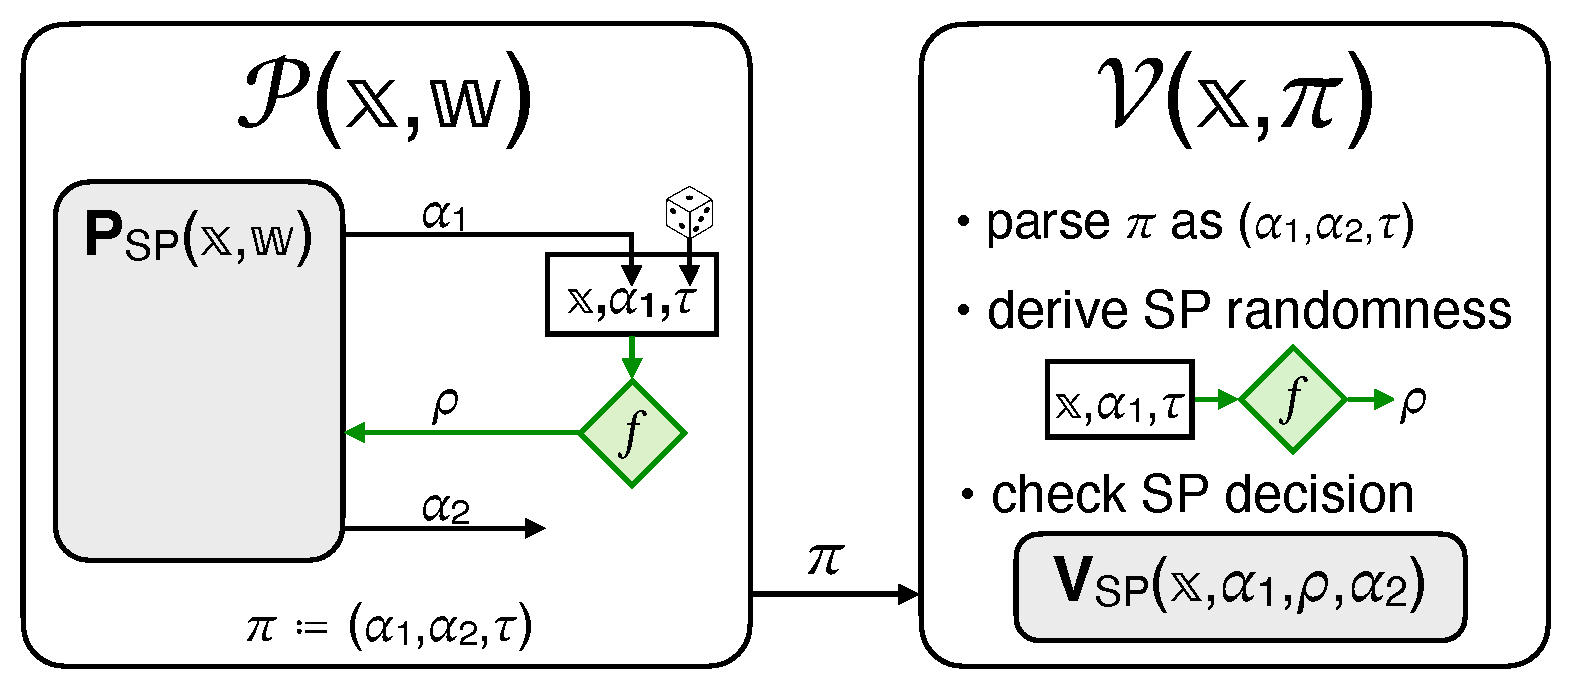
\includegraphics[width=0.7\textwidth]{\FigureFolder/fs-sp-diagram}
\caption[Diagram of the FS transformation for SPs]{Diagram of the \FSonSPText ($\FSonSPSymbol$ in \Cref{construction:fs-for-sp}).}
\label{figure:fs-for-sp-diagram}
\end{figure}

%%%%%%%%%%%%%%%%%%%%%%%%%%%%%%%%%%%%%%%%%%%%%%%%%%%%%%%%%%%%%%%%%%%%%%%%%%%%%%%
%%%%%%%%%%%%%%%%%%%%%%%%%%%%%%%%%%%%%%%%%%%%%%%%%%%%%%%%%%%%%%%%%%%%%%%%%%%%%%%
%%%%%%%%%%%%%%%%%%%%%%%%%%%%%%%%%%%%%%%%%%%%%%%%%%%%%%%%%%%%%%%%%%%%%%%%%%%%%%%
\section{Adaptive soundness}
\label{section:narg-from-sp-adaptive-soundness}

We prove that the adaptive soundness error of the non-interactive argument in \Cref{construction:fs-for-sp} is at most $\ROQueryBound+1$ times the soundness error of the underlying SP. This directly follows from a lemma that (efficiently) transforms a malicious argument prover into a malicious SP prover, with a loss of at most a factor of $\ROQueryBound+1$ in convincing probability.

\begin{ImportantTheorem}{}{narg-from-sp-adaptive-soundness}
Let $\SPSymbol=\SPSystem$ be an SP for a relation $\Relation$ with soundness error $\SPSoundnessError$. For every security parameter $\SecurityParameter \in \Naturals$ and privacy parameter $\PrivacyParameter \in \Naturals$, $\NARGSymbol \DefineEqual \FSonSPTransformation{\SPSymbol}{\SecurityParameter}{\PrivacyParameter}$ in \Cref{construction:fs-for-sp} is a non-interactive argument for $\Relation$ with adaptive soundness error $\ARGSoundnessError$ (see \Cref{definition:narg-adaptive-soundness-with-cnf}) such that
\begin{equation*}
\ARGSoundnessError(\SecurityParameter,\ROQueryBound,\InstanceSize)
\leq
(\ROQueryBound+1)
\cdot
\SPSoundnessError(\InstanceSize)
\enspace.
\end{equation*}
\end{ImportantTheorem}

\begin{lemma}
\label{lemma:fs-for-sigma-protocols-adaptive}
There exists an SP prover $\SPMaliciousProver$ such that for every instance size bound $\InstanceSize \in \Naturals$, query bound $\ROQueryBound \in \Naturals$, and malicious $\ROQueryBound$-query argument prover $\Malicious{\ARGProver}$,
\begin{align*}
&\Pr\left[
\begin{array}{l}
\SomeSize{\Instance} \leq \InstanceSize \\
\land\;\Instance \notin \GetLanguage{\Relation} \\
\land\;\ARGVerifier^{\ROFunction}(\Instance,\ARGString) = 1
\end{array}
\GivenExperiment
\StateExperiment{
\ROFunction \gets \RODistribution{\SPRandomnessComplexity} \\
(\Instance,\ARGString) \gets \Malicious{\ARGProver}^{\ROFunction}
}
\right]
\\&
\leq
(\ROQueryBound+1) \cdot
\Pr\left[
\begin{array}{l}
\SomeSize{\Instance} \leq \InstanceSize \\
\land\;\Instance \notin \GetLanguage{\Relation} \\
\land\;\SPVerifier(\Instance,\SPCommitment,\SPChallenge,\SPResponse)=1
\end{array}
\GivenExperiment
\StateExperiment{
(\Instance,\SPCommitment, \AuxiliaryState) \gets \SPMaliciousProver(\BlackBox{\Malicious{\ARGProver}}) \\
\SPChallenge \gets \Bits^{\SPRandomnessComplexity} \\
\SPResponse \gets \SPMaliciousProver(\AuxiliaryState, \SPChallenge)
}
\right]
\enspace.
\end{align*}
Moreover, if the running time of $\Malicious{\ARGProver}$ is $\ARGTimeP$ then the running time of $\SPMaliciousProver$ is $\ARGTimeP + O(\SPRandomnessComplexity \cdot \ROQueryBound)$.
\end{lemma}

\begin{construction}
\label{construction:fs-for-sigma-protocols-adaptive}
The SP prover $\SPMaliciousProver$ is parameterized by the query bound $\ROQueryBound$ and receives an argument prover $\Malicious{\ARGProver}$ as a black box, and works as follows.
\begin{itemize}[noitemsep]
  \item First SP prover message: $\SPMaliciousProver(\BlackBox{\Malicious{\ARGProver}}) \to (\Instance,\SPCommitment, \AuxiliaryState)$.
  \begin{enumerate}[noitemsep]
    \item Lazily sample an oracle $\Lazy{\ROFunction} \gets \RODistribution{\SPRandomnessComplexity}$.
    \item Sample an index $i \in [\ROQueryBound+1]$ at random.
    \item Simulate $\Malicious{\ARGProver}^{\Lazy{\ROFunction}}$ up to before the $i$-th unique query $\ROQuery$ to $\ROFunction$:
    \begin{enumerate}[noitemsep]
      \item If $\Malicious{\ARGProver}$ already stopped with output $(\Instance',(\SPCommitment',\SPResponse',\RandSaltString'))$, then set $\Instance \DefineEqual \Instance'$, $\RandSaltString \DefineEqual \RandSaltString'$, $\SPCommitment \DefineEqual \SPCommitment'$.
      \item Else if the query $\ROQuery$ can be parsed as $(\Instance_{i},\SPCommitmentIndexed{i},\RandSaltString_{i})$, then set $\Instance \DefineEqual \Instance_{i}$, $\RandSaltString \DefineEqual \RandSaltString_{i}$, $\SPCommitment \DefineEqual \SPCommitmentIndexed{i}$.
      \item Else set $\Instance \DefineEqual \bot$, $\RandSaltString \DefineEqual \bot$, $\SPCommitment \DefineEqual \bot$.
    \end{enumerate}
    \item Let $\AuxiliaryState_{\Malicious{\ARGProver}}$ be the state of $\Malicious{\ARGProver}$.
    \item Output the instance $\Instance$, first SP prover message $\SPCommitment$, and the auxiliary information $\AuxiliaryState \DefineEqual (\Lazy{\ROFunction},\Instance,\SPCommitment,\RandSaltString,\AuxiliaryState_{\Malicious{\ARGProver}})$.
  \end{enumerate}
  \item Second SP prover message: $\SPMaliciousProver(\AuxiliaryState=(\Lazy{\ROFunction},\Instance,\SPCommitment,\RandSaltString,\AuxiliaryState_{\Malicious{\ARGProver}}), \SPChallenge \in \Bits^{\SPRandomnessComplexity}) \to \SPResponse$.
  \begin{enumerate}[noitemsep]
    \item Set $\ARGZKProgrammedList \DefineEqual \{((\Instance,\SPCommitment,\RandSaltString),\SPChallenge)\}$.
    \item Use $\AuxiliaryState_{\Malicious{\ARGProver}}$ to continue the simulation of $\Malicious{\ARGProver}^{\ROProgram{\Lazy{\ROFunction}}{\ARGZKProgrammedList}}$ until it outputs $(\Instance',(\SPCommitment',\SPResponse',\RandSaltString'))$.
    \item If $\Instance' \neq \Instance \lor \SPCommitment' \neq \SPCommitment \lor \RandSaltString' \neq \RandSaltString$ set $\SPResponse \DefineEqual \bot$; otherwise set $\SPResponse \DefineEqual \SPResponse'$.
    \item Output the second SP prover message $\SPResponse$.
  \end{enumerate}
\end{itemize}
\end{construction}

\begin{proof}
The SP prover $\SPMaliciousProver$ simulates $\Malicious{\ARGProver}$ with a random function (sampled in a lazy way): $\SPMaliciousProver$ runs $\Malicious{\ARGProver}$ with the oracle $\ROProgram{\ROFunction}{\ARGZKProgrammedList}$, where $\ARGZKProgrammedList = \{((\Instance,\SPCommitment,\RandSaltString),\SPChallenge)\}$ programs $\ROFunction$ with the random answer $\SPChallenge$ for the query $(\Instance,\SPCommitment,\RandSaltString)$. Moreover, the choice of $i \in [\ROQueryBound+1]$ is independent of the execution of $\Malicious{\ARGProver}$. If $(\Instance',\SPCommitment',\RandSaltString') = (\Instance_{j},\SPCommitmentIndexed{j},\RandSaltString_{j})$ for some $j \in [\ROQueryBound]$ then $(\Instance',\SPCommitment',\RandSaltString') = (\Instance,\SPCommitment,\RandSaltString)$ if $\SPMaliciousProver$ sampled $i = j$ (note that in this case the query is well-formed and can be  parsed). Otherwise, if $(\Instance',\SPCommitment',\RandSaltString')$ is not a query in the query-answer trace, then $(\Instance',\SPCommitment',\RandSaltString') = (\Instance,\SPCommitment,\RandSaltString)$ if $\SPMaliciousProver$ sampled $i = \ROQueryBound+1$. We deduce that the probability that $(\Instance',\SPCommitment',\RandSaltString') = (\Instance,\SPCommitment,\RandSaltString)$, and thus that $\SPResponse \neq \bot$, is at least $\frac{1}{\ROQueryBound+1}$. Therefore, the following two distributions are equivalent:
\begin{equation}
\label{eq:sp-prover-equiv-dist}
\left\{
  (\Instance,\SPCommitment,\SPChallenge,\SPResponse)
\GivenExperiment
\StateExperiment{
  (\Instance, \SPCommitment, \AuxiliaryState) \gets \SPMaliciousProver(\BlackBox{\Malicious{\ARGProver}}) \\
  \SPChallenge \gets \Bits^{\SPRandomnessComplexity} \\
  \SPResponse \gets \SPMaliciousProver(\AuxiliaryState, \SPChallenge) \\
  \ConditionedOnText \\
  \SPResponse \neq \bot
}
\right\}
\equiv
\left\{
  (\Instance,\SPCommitment,\SPChallenge,\SPResponse)
\GivenExperiment
\StateExperiment{
  \ROFunction \gets \RODistribution{\SPRandomnessComplexity} \\
  (\Instance,\SPFSARGString) \gets \Malicious{\ARGProver}^{\ROFunction} \\
  \SPChallenge \DefineEqual \ROFunction(\Instance,\SPCommitment,\RandSaltString)
}
\right\}
\enspace.
\end{equation}
Moreover, we can lower bound the probability that $\SPResponse \neq \bot$ as follows:
\begin{equation}
\label{eq:sp-prover-guess-alpha}
\Pr\left[
  \SPResponse \neq \bot
\GivenExperiment
\StateExperiment{
  (\Instance, \SPCommitment, \AuxiliaryState) \gets \SPMaliciousProver(\BlackBox{\Malicious{\ARGProver}}) \\
  \SPChallenge \gets \Bits^{\SPRandomnessComplexity} \\
  \SPResponse \gets \SPMaliciousProver(\AuxiliaryState, \SPChallenge)
}
\right]
\geq
\frac{1}{\ROQueryBound+1}
\enspace.
\end{equation}
Using the above, we conclude that
\begin{align*}
& \Pr\left[
\begin{array}{l}
\SomeSize{\Instance} \leq \InstanceSize \\
\land\;\Instance \notin \GetLanguage{\Relation} \\
\land\;\SPVerifier(\Instance,\SPCommitment,\SPChallenge,\SPResponse)=1
\end{array}
\GivenExperiment
\StateExperiment{
(\Instance, \SPCommitment, \AuxiliaryState) \gets \SPMaliciousProver(\BlackBox{\Malicious{\ARGProver}}) \\
\SPChallenge \gets \Bits^{\SPRandomnessComplexity} \\
\SPResponse \gets \SPMaliciousProver(\AuxiliaryState, \SPChallenge)
}
\right]
\\ & \geq
\Pr\left[
\SPResponse \neq \bot
\GivenExperiment
\StateExperiment{
(\Instance, \SPCommitment, \AuxiliaryState) \gets \SPMaliciousProver(\BlackBox{\Malicious{\ARGProver}}) \\
\SPChallenge \gets \Bits^{\SPRandomnessComplexity} \\
\SPResponse \gets \SPMaliciousProver(\AuxiliaryState, \SPChallenge)
}
\right]
\\ & \phantom{aaaaa} \cdot
\Pr\left[
\begin{array}{l}
\SomeSize{\Instance} \leq \InstanceSize \\
\land\;\Instance \notin \GetLanguage{\Relation} \\
\land\;\SPVerifier(\Instance,\SPCommitment,\SPChallenge,\SPResponse)=1 \\
\ConditionedOnText \\
\SPResponse \neq \bot
\end{array}
\GivenExperiment
\StateExperiment{
(\Instance, \SPCommitment, \AuxiliaryState) \gets \SPMaliciousProver(\BlackBox{\Malicious{\ARGProver}}) \\
\SPChallenge \gets \Bits^{\SPRandomnessComplexity} \\
\SPResponse \gets \SPMaliciousProver(\AuxiliaryState, \SPChallenge)
}
\right]
\\ & \geq
\frac{1}{\ROQueryBound+1} \cdot
\Pr\left[
\begin{array}{l}
\SomeSize{\Instance} \leq \InstanceSize \\
\land\;\Instance \notin \GetLanguage{\Relation} \\
\land\;\SPVerifier(\Instance,\SPCommitment,\ROFunction(\Instance,\SPCommitment,\RandSaltString),\SPResponse)=1
\end{array}
\GivenExperiment
\StateExperiment{
\ROFunction \gets \RODistribution{\SPRandomnessComplexity} \\
(\Instance,(\SPCommitment,\SPResponse,\RandSaltString)) \gets \Malicious{\ARGProver}^{\ROFunction}
}
\right]
\\ & =
\frac{1}{\ROQueryBound+1} \cdot
\Pr\left[
\begin{array}{l}
\SomeSize{\Instance} \leq \InstanceSize \\
\land\;\Instance \notin \GetLanguage{\Relation} \\
\land\;\ARGVerifier^{\ROFunction}(\Instance,\ARGString) = 1
\end{array}
\GivenExperiment
\StateExperiment{
\ROFunction \gets \RODistribution{\SPRandomnessComplexity} \\
(\Instance,\ARGString) \gets \Malicious{\ARGProver}^{\ROFunction}
}
\right]
\enspace.
\end{align*}
\end{proof}

















































































































%%%%%%%%%%%%%%%%%%%%%%%%%%%%%%%%%%%%%%%%%%%%%%%%%%%%%%%%%%%%%%%%%%%%%%%%%%%%%%%
%%%%%%%%%%%%%%%%%%%%%%%%%%%%%%%%%%%%%%%%%%%%%%%%%%%%%%%%%%%%%%%%%%%%%%%%%%%%%%%
%%%%%%%%%%%%%%%%%%%%%%%%%%%%%%%%%%%%%%%%%%%%%%%%%%%%%%%%%%%%%%%%%%%%%%%%%%%%%%%
%%%%%%%%%%%%%%%%%%%%%%%%%%%%%%%%%%%%%%%%%%%%%%%%%%%%%%%%%%%%%%%%%%%%%%%%%%%%%%%
\chapter{Additional security definitions}
\label{chapter:fs-for-sp-additional}

We prove that \Cref{construction:fs-for-sp} satisfies additional security definitions.

%%%%%%%%%%%%%%%%%%%%%%%%%%%%%%%%%%%%%%%%%%%%%%%%%%%%%%%%%%%%%%%%%%%%%%%%%%%%%%%
%%%%%%%%%%%%%%%%%%%%%%%%%%%%%%%%%%%%%%%%%%%%%%%%%%%%%%%%%%%%%%%%%%%%%%%%%%%%%%%
%%%%%%%%%%%%%%%%%%%%%%%%%%%%%%%%%%%%%%%%%%%%%%%%%%%%%%%%%%%%%%%%%%%%%%%%%%%%%%%
\section{Knowledge soundness}
\label{section:fs-sigma-protocol-adaptive-knowledge-soundness}

In \Cref{construction:fs-for-sp}, if the SP satisfies knowledge soundness then the resulting non-interactive argument satisfies adaptive knowledge soundness.

\begin{ImportantTheorem}{}{narg-from-sp-adaptive-knowledge-soundness}
Let $\SPSymbol=\SPSystem$ be an SP for a relation $\Relation$ with rewinding knowledge soundness error $\SPKnowledgeError$ with extraction time $\SPKnowledgeTime$ (see \Cref{definition:sp-knowledge-soundness}). For every security parameter $\SecurityParameter \in \Naturals$ and privacy parameter $\PrivacyParameter \in \Naturals$, $\NARGSymbol \DefineEqual \FSonSPTransformation{\SPSymbol}{\SecurityParameter}{\PrivacyParameter}$ in \Cref{construction:fs-for-sp} is a non-interactive argument for $\Relation$ with rewinding knowledge soundness error $\ARGKnowledgeError$ with extraction time $\ARGKnowledgeTime$ (see \Cref{definition:adaptive-rewinding-knowledge-soundness-with-cnf}) such that
\begin{itemize}[nolistsep]

  \item $\ARGKnowledgeError(\SecurityParameter,\ROQueryBound,\InstanceSize,\ProverFailureProbability{\Malicious{\ARGProver}}(\SecurityParameter,\InstanceSize))\leq(\ROQueryBound+1) \cdot \SPKnowledgeError\left(\InstanceSize,\ProverFailureProbabilityPrime{\Malicious{\ARGProver}}(\SecurityParameter,\InstanceSize)\right)$, and

  \item $\ARGKnowledgeTime(\SecurityParameter,\ROQueryBound,\InstanceSize,\ProverFailureProbability{\Malicious{\ARGProver}}(\SecurityParameter,\InstanceSize),\ProverRunningTime{\Malicious{\ARGProver}}(\SecurityParameter,\InstanceSize)) \leq \SPKnowledgeTime\left(\InstanceSize,\ProverFailureProbabilityPrime{\Malicious{\ARGProver}}(\SecurityParameter,\InstanceSize),\ProverRunningTimePrime{\Malicious{\ARGProver}}(\SecurityParameter,\InstanceSize)\right)$.

\end{itemize}
Above, $\ProverFailureProbabilityPrime{\Malicious{\ARGProver}}(\SecurityParameter,\InstanceSize) \DefineEqual 1-\frac{1-\ProverFailureProbability{\Malicious{\ARGProver}}(\SecurityParameter,\InstanceSize)}{\ROQueryBound+1}$ and $\ProverRunningTimePrime{\Malicious{\ARGProver}}(\SecurityParameter,\InstanceSize) \DefineEqual \ProverRunningTime{\Malicious{\ARGProver}}(\SecurityParameter,\InstanceSize)+O(\SPRandomnessComplexity \cdot \ROQueryBound)$.

Moreover, if the SP extractor is straightline then the NARG extractor is also straightline (see \Cref{definition:adaptive-straightline-knowledge-soundness-with-cnf}). In this case:
\begin{itemize}[nolistsep]
  \item the (straightline) knowledge soundness error is $\ARGKnowledgeError(\SecurityParameter,\ROQueryBound,\InstanceSize)\leq(\ROQueryBound+1) \cdot \SPKnowledgeError(\InstanceSize)$; and
  \item the (straightline) extraction time is $\ARGKnowledgeTime(\SecurityParameter,\ROQueryBound,\InstanceSize) \leq \SPKnowledgeTime(\InstanceSize)$.
\end{itemize}
\end{ImportantTheorem}

The theorem directly follows from the lemma below.

\begin{lemma}
\label{lemma:fs-for-sp-adaptive-knowledge-soundness}
Let $\SPExtractor$ be the SP extractor for $\SPSymbol=\SPSystem$. There exists an argument extractor $\ARGExtractor$ such that for every query bound $\ROQueryBound \in \Naturals$, malicious $\ROQueryBound$-query argument prover $\Malicious{\ARGProver}$, and instance size bound $\InstanceSize \in \Naturals$,
\begin{align*}
& \Pr\left[
\begin{array}{l}
  \SomeSize{\Instance} \leq \InstanceSize \\
  \land\;(\Instance,\Witness) \notin \Relation \\
  \land\;\DecisionBit = 1
\end{array}
\GivenExperiment
\StateExperiment{
  \ROFunction \gets \RODistribution{\SPRandomnessComplexity} \\
  (\Instance, \ARGString) \xleftarrow{\ROTrace} \Malicious{\ARGProver}^{\ROFunction} \\
  \DecisionBit \xleftarrow{\ROTraceVerifier} \ARGVerifier^{\ROFunction}(\Instance,\ARGString) \\
  \Witness \gets \ARGExtractor(\Instance,\ARGString,\ROTrace,\ROTraceVerifier,\BlackBox{\Malicious{\ARGProver}})
}
\right]
\\ & \leq
(\ROQueryBound+1) \cdot
\Pr\left[
\begin{array}{l}
  \SomeSize{\Instance} \leq \InstanceSize \\
  \land\;(\Instance,\Witness) \notin \Relation \\
  \land\;\SPVerifier(\Instance,\SPCommitment,\SPChallenge,\SPResponse)=1
\end{array}
\GivenExperiment
\StateExperiment{
  (\Instance, \SPCommitment, \AuxiliaryState) \gets \SPMaliciousProver(\BlackBox{\Malicious{\ARGProver}}) \\
  \SPChallenge \gets \Bits^{\SPRandomnessComplexity} \\
  \SPResponse \gets \SPMaliciousProver(\AuxiliaryState, \SPChallenge) \\
  \Witness \gets \SPExtractor(\Instance,\SPCommitment,\SPChallenge,\SPResponse,\BlackBox{\SPMaliciousProver})
}
\right]
\enspace.
\end{align*}
Moreover, the running time of $\ARGExtractor$ is $\SPKnowledgeTime\left(\InstanceSize,1-\frac{1-\ProverFailureProbability{\Malicious{\ARGProver}}(\SecurityParameter,\Instance)}{\ROQueryBound+1},\ProverRunningTime{\Malicious{\ARGProver}}(\SecurityParameter,\Instance)+O(\SPRandomnessComplexity \cdot \ROQueryBound)\right)$.
\end{lemma}

\begin{construction}
\label{construction:fs-for-sp-adaptive-extractor}
The argument extractor $\ARGExtractor$ receives as input an instance $\Instance$, argument string $\ARGString$, query-answer trace $\ROTrace$ of the argument prover, query-answer trace $\ROTraceVerifier$ of the argument verifier, and black-box access to the argument prover $\Malicious{\ARGProver}$, and works as follows.
\begin{itemize}[noitemsep]
\item[] $\ARGExtractor(\Instance,\ARGString,\ROTrace,\ROTraceVerifier,\BlackBox{\Malicious{\ARGProver}})$:
\begin{enumerate}[nolistsep]
  \item Parse the argument string $\ARGString$ as a tuple $\SPFSARGString$.
  \item Parse the query-answer trace $\ROTraceVerifier$ of the argument verifier as a single pair $((\Instance,\SPCommitment,\RandSaltString),\SPChallenge)$.
  \item Let $\SPMaliciousProver \DefineEqual \SPMaliciousProver(\BlackBox{\Malicious{\ARGProver}})$ be the SP prover in \Cref{construction:fs-for-sp-efficient-reduction}.
  \item Compute the witness: $\Witness \gets \SPExtractor(\Instance,\SPCommitment,\SPChallenge,\SPResponse,\SPMaliciousProver(\BlackBox{\Malicious{\ARGProver}}))$.
  \item Output $\Witness$.
\end{enumerate}
\end{itemize}
\end{construction}

\begin{proof}
We upper bound the rewinding knowledge soundness error. Note that $\ARGVerifier$ invokes the random oracle $\ROFunction$ once only: the query $(\Instance,\SPCommitment,\RandSaltString)$, which is answered via $\SPChallenge \DefineEqual \ROFunction(\Instance,\SPCommitment,\RandSaltString)$. We can write
\begin{align*}
& \Pr\left[
\begin{array}{l}
  \SomeSize{\Instance} \leq \InstanceSize \\
  \land\;(\Instance,\Witness) \notin \Relation \\
  \land\;\DecisionBit = 1
\end{array}
\GivenExperiment
\StateExperiment{
  \ROFunction \gets \RODistribution{\SecurityParameter} \\
  \ROOutputAndTrace{\ROFunction}{\Malicious{\ARGProver}}{\ROTrace}{(\Instance,\ARGString)} \\
  \DecisionBit \xleftarrow{\ROTraceVerifier} \ARGVerifier^{\ROFunction}(\Instance,\ARGString) \\
  \Witness \gets \ARGExtractor(\Instance,\ARGString,\ROTrace,\ROTraceVerifier,\BlackBox{\Malicious{\ARGProver}})
}
\right]
\\ & =
\Pr\left[
\begin{array}{l}
  \SomeSize{\Instance} \leq \InstanceSize \\
  \land\;(\Instance,\Witness) \notin \Relation \\
  \land\;\SPVerifier(\Instance,\SPCommitment,\SPChallenge,\SPResponse)=1
\end{array}
\GivenExperiment
\StateExperiment{
  \ROFunction \gets \RODistribution{\SecurityParameter} \\
  \ROOutputAndTrace{\ROFunction}{\Malicious{\ARGProver}}{\ROTrace}{(\Instance,\SPFSARGString)} \\
  \SPChallenge \DefineEqual \ROFunction(\Instance,\SPCommitment,\RandSaltString) \\
  \Witness \gets \SPExtractor(\Instance,\SPCommitment,\SPChallenge,\SPResponse,\SPMaliciousProver(\BlackBox{\Malicious{\ARGProver}}))
}
\right]
\EquationComment{by definition of $\ARGExtractor$}
\\ & =
\Pr\left[
\begin{array}{l}
  \SomeSize{\Instance} \leq \InstanceSize \\
  \land\;(\Instance,\Witness) \notin \Relation \\
  \land\;\SPVerifier(\Instance,\SPCommitment,\SPChallenge,\SPResponse)=1 \\
  \ConditionedOnText \\
  \SPResponse \neq \bot
\end{array}
\GivenExperiment
\StateExperiment{
  (\Instance, \SPCommitment, \AuxiliaryState) \gets \SPMaliciousProver(\BlackBox{\Malicious{\ARGProver}}) \\
  \SPChallenge \gets \Bits^{\SPRandomnessComplexity} \\
  \SPResponse \gets \SPMaliciousProver(\AuxiliaryState, \SPChallenge) \\
  \Witness \gets \SPExtractor(\Instance,\SPCommitment,\SPChallenge,\SPResponse,\BlackBox{\SPMaliciousProver})
}
\right]
\EquationComment{by \Cref{eq:sp-prover-equiv-dist}}
\\ & =
\Pr\left[
\begin{array}{l}
  \SomeSize{\Instance} \leq \InstanceSize \\
  \land\;(\Instance,\Witness) \notin \Relation \\
  \land\;\SPVerifier(\Instance,\SPCommitment,\SPChallenge,\SPResponse)=1 \\
  \land\; \SPResponse \neq \bot
\end{array}
\GivenExperiment
\StateExperiment{
  (\Instance, \SPCommitment, \AuxiliaryState) \gets \SPMaliciousProver(\BlackBox{\Malicious{\ARGProver}}) \\
  \SPChallenge \gets \Bits^{\SPRandomnessComplexity} \\
  \SPResponse \gets \SPMaliciousProver(\AuxiliaryState, \SPChallenge) \\
  \Witness \gets \SPExtractor(\Instance,\SPCommitment,\SPChallenge,\SPResponse,\BlackBox{\SPMaliciousProver})
}
\right]
\\ & \phantom{aaa} \Big /
\Pr\left[
  \SPResponse \neq \bot
\GivenExperiment
\StateExperiment{
  (\Instance, \SPCommitment, \AuxiliaryState) \gets \SPMaliciousProver(\BlackBox{\Malicious{\ARGProver}}) \\
  \SPChallenge \gets \Bits^{\SPRandomnessComplexity} \\
  \SPResponse \gets \SPMaliciousProver(\AuxiliaryState, \SPChallenge)
}
\right]
\\ & \leq
(\ROQueryBound +1) \cdot
\Pr\left[
\begin{array}{l}
  \SomeSize{\Instance} \leq \InstanceSize \\
  \land\;(\Instance,\Witness) \notin \Relation \\
  \land\;\SPVerifier(\Instance,\SPCommitment,\SPChallenge,\SPResponse)=1
\end{array}
\GivenExperiment
\StateExperiment{
  (\Instance, \SPCommitment, \AuxiliaryState) \gets \SPMaliciousProver(\BlackBox{\Malicious{\ARGProver}}) \\
  \SPChallenge \gets \Bits^{\SPRandomnessComplexity} \\
  \SPResponse \gets \SPMaliciousProver(\AuxiliaryState, \SPChallenge) \\
  \Witness \gets \SPExtractor(\Instance,\SPCommitment,\SPChallenge,\SPResponse,\BlackBox{\SPMaliciousProver})
}
\right]
\enspace.
\end{align*}
The last inequality comes from \Cref{eq:sp-prover-guess-alpha} and the fact that $\SPVerifier(\Instance,\SPCommitment,\SPChallenge,\SPResponse)=1$ implies that $\SPResponse \neq \bot$.

Next, we discuss the running time of $\ARGExtractor$. This depends on the running time of $\SPExtractor$, which in turn depends on the failure probability and running time of $\SPMaliciousProver(\BlackBox{\Malicious{\ARGProver}})$. Observe that \Cref{lemma:fs-for-sigma-protocols-adaptive} does not suffice to upper bound the failure probability of $\SPMaliciousProver(\BlackBox{\Malicious{\ARGProver}})$, because the probability events in the lemma include the condition $\Instance \notin \GetLanguage{\Relation}$, while the failure probability does not include this condition. Nevertheless, using \Cref{eq:sp-prover-equiv-dist,eq:sp-prover-guess-alpha} in the proof of \Cref{lemma:fs-for-sigma-protocols-adaptive}, we can straightforwardly upper bound the failure probability (by lower bounding the success probability):
\begin{align*}
& \Pr\left[
\begin{array}{l}
  \SomeSize{\Instance} \leq \InstanceSize \\
  \land\;\SPVerifier(\Instance,\SPCommitment,\SPChallenge,\SPResponse)=1
\end{array}
\GivenExperiment
\StateExperiment{
  (\Instance, \SPCommitment, \AuxiliaryState) \gets \SPMaliciousProver(\BlackBox{\Malicious{\ARGProver}}) \\
  \SPChallenge \gets \Bits^{\SPRandomnessComplexity} \\
  \SPResponse \gets \SPMaliciousProver(\AuxiliaryState, \SPChallenge)
}
\right]
\\ & \geq
\Pr\left[
\SPResponse \neq \bot
\GivenExperiment
\StateExperiment{
  (\Instance, \SPCommitment, \AuxiliaryState) \gets \SPMaliciousProver(\BlackBox{\Malicious{\ARGProver}}) \\
  \SPChallenge \gets \Bits^{\SPRandomnessComplexity} \\
  \SPResponse \gets \SPMaliciousProver(\AuxiliaryState, \SPChallenge)
}
\right]
\\ &\phantom{aaaaa}\cdot
\Pr\left[
\begin{array}{l}
  \SomeSize{\Instance} \leq \InstanceSize \\
  \land\;\SPVerifier(\Instance,\SPCommitment,\SPChallenge,\SPResponse)=1 \\
  \ConditionedOnText \\
  \SPResponse \neq \bot
\end{array}
\GivenExperiment
\StateExperiment{
  (\Instance, \SPCommitment, \AuxiliaryState) \gets \SPMaliciousProver(\BlackBox{\Malicious{\ARGProver}}) \\
  \SPChallenge \gets \Bits^{\SPRandomnessComplexity} \\
  \SPResponse \gets \SPMaliciousProver(\AuxiliaryState, \SPChallenge)
}
\right]
\\ & \geq
\frac{1}{\ROQueryBound+1} \cdot
\Pr\left[
\begin{array}{l}
  \SomeSize{\Instance} \leq \InstanceSize \\
  \land\;\SPVerifier(\Instance,\SPCommitment,\ROFunction(\Instance,\SPCommitment,\RandSaltString),\SPResponse)=1
\end{array}
\GivenExperiment
\StateExperiment{
  \ROFunction \gets \RODistribution{\SPRandomnessComplexity} \\
  (\Instance,(\SPCommitment,\SPResponse,\RandSaltString)) \gets \Malicious{\ARGProver}^{\ROFunction}
}
\right]
\\ & =
\frac{1}{\ROQueryBound+1} \cdot
\Pr\left[
\begin{array}{l}
  \SomeSize{\Instance} \leq \InstanceSize \\
  \land\;\ARGVerifier^{\ROFunction}(\Instance,\ARGString)=1
\end{array}
\GivenExperiment
\StateExperiment{
  \ROFunction \gets \RODistribution{\SPRandomnessComplexity} \\
  (\Instance,\ARGString) \gets \Malicious{\ARGProver}^{\ROFunction}
}
\right]
\enspace.
\end{align*}
Taking the complement events and rearranging:
\begin{align*}
& \Pr\left[
\begin{array}{l}
  \SomeSize{\Instance} > \InstanceSize \\
  \lor\;\SPVerifier(\Instance,\SPCommitment,\SPChallenge,\SPResponse)=0
\end{array}
\GivenExperiment
\StateExperiment{
  (\Instance, \SPCommitment, \AuxiliaryState) \gets \SPMaliciousProver(\BlackBox{\Malicious{\ARGProver}}) \\
  \SPChallenge \gets \Bits^{\SPRandomnessComplexity} \\
  \SPResponse \gets \SPMaliciousProver(\AuxiliaryState, \SPChallenge)
}
\right]
\\ & \leq
1-
\frac{1}{\ROQueryBound+1} \cdot
\left(
1-
\Pr\left[
\begin{array}{l}
  \SomeSize{\Instance} > \InstanceSize \\
  \lor\;\ARGVerifier^{\ROFunction}(\Instance,\ARGString)=0
\end{array}
\GivenExperiment
\StateExperiment{
  \ROFunction \gets \RODistribution{\SPRandomnessComplexity} \\
  (\Instance,\ARGString) \gets \Malicious{\ARGProver}^{\ROFunction}
}
\right]
\right)
\\ & =
1-
\frac{1}{\ROQueryBound+1} \cdot
\left(
1-\ProverFailureProbability{\Malicious{\ARGProver}}(\SecurityParameter,\InstanceSize)
\right)
\enspace.
\end{align*}
We deduce that the failure probability of $\SPMaliciousProver(\BlackBox{\Malicious{\ARGProver}})$ is $\ProverFailureProbabilityPrime{\Malicious{\ARGProver}}(\SecurityParameter,\InstanceSize) \DefineEqual 1-\frac{1-\ProverFailureProbability{\Malicious{\ARGProver}}(\SecurityParameter,\InstanceSize)}{\ROQueryBound+1}$. Moreover, by inspection of \Cref{construction:fs-for-sp-efficient-reduction}, the running time of $\SPMaliciousProver(\BlackBox{\Malicious{\ARGProver}})$ is $\ProverRunningTimePrime{\Malicious{\ARGProver}}(\SecurityParameter,\InstanceSize) \DefineEqual \ProverRunningTime{\Malicious{\ARGProver}}(\SecurityParameter,\InstanceSize)+O(\SPRandomnessComplexity \cdot \ROQueryBound)$. Therefore, the running time of the SP extractor $\SPExtractor$, as invoked by $\ARGExtractor$, is $\SPKnowledgeTime\left(\InstanceSize,\ProverFailureProbabilityPrime{\Malicious{\ARGProver}}(\SecurityParameter,\InstanceSize),\ProverRunningTimePrime{\Malicious{\ARGProver}}(\SecurityParameter,\InstanceSize)\right)$. All other operations in $\ARGExtractor$ are merely syntactic.
\end{proof}

We conclude by discussing the special case of straightline extraction. Suppose that $\SPExtractor$ is a straightline extractor, which means that $\SPExtractor$ is a deterministic algorithm that does not receive as input the SP prover $\SPMaliciousProver$. Then $\ARGExtractor$ in \Cref{construction:fs-for-sp-adaptive-extractor} is a straightline extractor because $\ARGExtractor$ uses $\Malicious{\ARGProver}$ only to construct $\SPMaliciousProver(\BlackBox{\Malicious{\ARGProver}})$, which $\SPExtractor$ no longer needs. In this case, $\SPKnowledgeError$ does not depend on the failure probability of $\SPMaliciousProver$, so the knowledge soundness error bound simplifies to $\ARGKnowledgeError(\SecurityParameter,\ROQueryBound,\InstanceSize)\leq(\ROQueryBound+1) \cdot \SPKnowledgeError(\InstanceSize)$. Similarly, $\SPKnowledgeTime$ does not depend on the failure probability or running time of $\SPMaliciousProver$, so the extraction time bound simplifies to $\ARGKnowledgeTime(\SecurityParameter,\ROQueryBound,\InstanceSize) \leq \SPKnowledgeTime(\InstanceSize)$.

%%%%%%%%%%%%%%%%%%%%%%%%%%%%%%%%%%%%%%%%%%%%%%%%%%%%%%%%%%%%%%%%%%%%%%%%%%%%%%%
%%%%%%%%%%%%%%%%%%%%%%%%%%%%%%%%%%%%%%%%%%%%%%%%%%%%%%%%%%%%%%%%%%%%%%%%%%%%%%%
%%%%%%%%%%%%%%%%%%%%%%%%%%%%%%%%%%%%%%%%%%%%%%%%%%%%%%%%%%%%%%%%%%%%%%%%%%%%%%%
\section{Zero knowledge}
\label{section:narg-from-sp-zero-knowledge}

In \Cref{construction:fs-for-sp}, if the SP satisfies honest-verifier zero knowledge (and the privacy parameter $\PrivacyParameter$ of the construction is large enough), then the resulting non-interactive argument satisfies adaptive zero knowledge.

\begin{ImportantTheorem}{}{narg-from-sp-zero-knowledge}
Let $\SPSymbol$ be an SP for a relation $\Relation$ with honest-verifier zero-knowledge error $\SPZKError$ (see \Cref{definition:sp-hvzk}). For every security parameter $\SecurityParameter \in \Naturals$ and privacy parameter $\PrivacyParameter \in \Naturals$, \Cref{construction:fs-for-sp} is a non-interactive argument for $\Relation$ with adaptive zero-knowledge error $\ARGZKError$ (see \Cref{definition:once-adaptive-zk-narg-with-cnf}) such that
\begin{equation*}
\ARGZKError(\SecurityParameter,\ROQueryBound,\InstanceSize)
\leq
\FSSPZKExpression
\enspace.
\end{equation*}
\end{ImportantTheorem}

\begin{construction}
\label{construction:narg-from-sp-simulator}
The simulator is an algorithm $\ARGSimulator^{\ROFunction}(\Instance)$ that works as follows. Below we denote by $\SPSimulator$ the honest-verifier zero-knowledge simulator of the SP (see \Cref{definition:sp-hvzk}).
\begin{itemize}
  \item $\ARGSimulator^{\ROFunction}(\Instance)$:
  \begin{enumerate}[nolistsep]
    \item \label{step:narg-from-sp-zksimulator:sample-view}
    Sample a simulated view of the SP verifier: $(\Instance,\SPCommitment,\SPChallenge,\SPResponse) \gets \SPSimulator(\Instance)$.
    \item Sample a random salt $\RandSaltString \in \Bits^{\RandSaltSize}$.
    \item Set the argument string $\ARGString \DefineEqual \SPFSARGString$.
    \item \label{step:narg-from-sp-zksimulator:add-randomness}
    Set the list of query-answer pairs $\ARGZKProgrammedList \DefineEqual \{((\Instance,\SPCommitment,\RandSaltString),\SPChallenge)\}$.
    \item Output $(\ARGString,\ARGZKProgrammedList)$.
  \end{enumerate}
\end{itemize}
Note that $\ARGSimulator$ programs the oracle $\ROFunction$ at one point via the output $\ARGZKProgrammedList$ (and does not query $\ROFunction$).
\end{construction}

\begin{proof}
Fix a query bound $\ROQueryBound \in \Naturals$, $\ROQueryBound$-query admissible adversary $\ARGAdversary$, and instance bound $\InstanceSize \in \Naturals$. We wish to upper bound the statistical distance between the output of $\ARGAdversary$ in the real world and in the simulated world. For that, we introduce a hybrid simulator (that takes the witness as input and programs the oracle): $\ARGSimulatorHybrid^{\ROFunction}(\Instance,\Witness)$ acts as $\ARGSimulator^{\ROFunction}(\Instance)$ except that the view in \Cref{step:narg-from-sp-zksimulator:sample-view} is sampled as a real view $\SPSampledView \gets \SPView{\SPProver}{\SPVerifier}{\Instance}{\Witness}$. We list the real-world, hybrid-world, and simulated-world distributions, making explicit the operations underlying the relevant algorithms.
\begin{enumerate}
  \item The real-world distribution:
\begin{equation*}
\Distribution_{\RealSymbol}
\DefineEqual
\left\{
\ARGOutput
\GivenExperiment
\StateExperiment{
\ROFunction \gets \RODistribution{\SPRandomnessComplexity} \\
(\Instance,\Witness,\ROAdvState) \gets \ARGAdversary^{\ROFunction} \\
\Paint{\ARGString \gets \ARGProver^{\ROFunction}(\Instance,\Witness)} \\
\ARGOutput \gets \ARGAdversary^{\ROFunction}(\ROAdvState,\ARGString)
}
\right\}
\equiv
\left\{
\ARGOutput
\GivenExperiment
\StateExperiment{
\ROFunction \gets \RODistribution{\SPRandomnessComplexity} \\
(\Instance,\Witness,\ROAdvState) \gets \ARGAdversary^{\ROFunction} \\
\Paint{(\SPCommitment,\AuxiliaryState) \gets \SPProver(\Instance,\Witness)} \\
\Paint{\RandSaltString \gets \Bits^{\RandSaltSize}} \\
\Paint{\SPChallenge \DefineEqual \ROFunction(\Instance,\SPCommitment,\RandSaltString)} \\
\Paint{\SPResponse \gets \SPProver(\AuxiliaryState,\SPChallenge)} \\
\Paint{\ARGString \DefineEqual \SPFSARGString} \\
\ARGOutput \gets \ARGAdversary^{\ROFunction}(\ROAdvState,\ARGString)
}
\right\}
\enspace.
\end{equation*}

  \item The hybrid-world distribution:
\begin{equation*}
\Distribution_{\mathrm{H}}
\DefineEqual
\left\{
\ARGOutput
\GivenExperiment
\StateExperiment{
\ROFunction \gets \RODistribution{\SPRandomnessComplexity} \\
(\Instance,\Witness,\ROAdvState) \gets \ARGAdversary^{\ROFunction} \\
\Paint{(\ARGString,\ARGZKProgrammedList) \gets \ARGSimulatorHybrid^{\ROFunction}(\Instance,\Witness)} \\
\ARGOutput \gets \ARGAdversary^{\ROProgram{\ROFunction}{\ARGZKProgrammedList}}(\ROAdvState,\ARGString)
}
\right\}
\equiv
\left\{
\ARGOutput
\GivenExperiment
\StateExperiment{
\ROFunction \gets \RODistribution{\SPRandomnessComplexity} \\
(\Instance,\Witness,\ROAdvState) \gets \ARGAdversary^{\ROFunction} \\
\Paint{(\SPCommitment,\AuxiliaryState) \gets \SPProver(\Instance,\Witness)} \\
\Paint{\SPChallenge \gets \Bits^{\SPRandomnessComplexity}} \\
\Paint{\SPResponse \gets \SPProver(\AuxiliaryState,\SPChallenge)} \\
\Paint{\RandSaltString \gets \Bits^{\RandSaltSize}} \\
\Paint{\ARGString \DefineEqual \SPFSARGString} \\
\Paint{\ARGZKProgrammedList \DefineEqual \{((\Instance,\SPCommitment,\RandSaltString),\SPChallenge)\}} \\
\ARGOutput \gets \ARGAdversary^{\ROProgram{\ROFunction}{\ARGZKProgrammedList}}(\ROAdvState,\ARGString)
}
\right\}
\enspace.
\end{equation*}

  \item The simulated-world distribution:
\begin{equation*}
\Distribution_{\SimSymbol}
\DefineEqual
\left\{
\ARGOutput
\GivenExperiment
\StateExperiment{
\ROFunction \gets \RODistribution{\SPRandomnessComplexity} \\
(\Instance,\Witness,\ROAdvState) \gets \ARGAdversary^{\ROFunction} \\
\Paint{(\ARGString,\ARGZKProgrammedList) \gets \ARGSimulator^{\ROFunction}(\Instance)} \\
\ARGOutput \gets \ARGAdversary^{\ROProgram{\ROFunction}{\ARGZKProgrammedList}}(\ROAdvState,\ARGString)
}
\right\}
\equiv
\left\{
\ARGOutput
\GivenExperiment
\StateExperiment{
\ROFunction \gets \RODistribution{\SPRandomnessComplexity} \\
(\Instance,\Witness,\ROAdvState) \gets \ARGAdversary^{\ROFunction} \\
\Paint{(\Instance,\SPCommitment,\SPChallenge,\SPResponse) \gets \SPSimulator(\Instance)} \\
\Paint{\RandSaltString \gets \Bits^{\RandSaltSize}} \\
\Paint{\ARGString \DefineEqual \SPFSARGString} \\
\Paint{\ARGZKProgrammedList \DefineEqual \{((\Instance,\SPCommitment,\RandSaltString),\SPChallenge)\}} \\
\ARGOutput \gets \ARGAdversary^{\ROProgram{\ROFunction}{\ARGZKProgrammedList}}(\ROAdvState,\ARGString)
}
\right\}
\enspace.
\end{equation*}

\end{enumerate}
Next we analyze the statistical difference between these distributions.
\begin{itemize}

\item \emph{Real versus hybrid.}
We analyze the statistical distance between $\Distribution_{\RealSymbol}$ and $\Distribution_{\mathrm{H}}$.

The two distributions only differ in that the hybrid simulator $\ARGSimulatorHybrid$ programs the oracle $\ROFunction$ by setting the answer to the query $(\Instance,\SPCommitment,\RandSaltString)$ to be a freshly sampled SP challenge $\SPChallenge$ (independent of $\ROFunction$), whereas the argument prover $\ARGProver$ does not program the oracle (it sets $\SPChallenge$ to be the answer of $\ROFunction$ to the query $(\Instance,\SPCommitment,\RandSaltString)$).

The distribution of $((\Instance,\SPCommitment,\RandSaltString),\SPChallenge)$ is the same in both cases. However, $\ARGAdversary$ has access to $\ROFunction$ before $\ROFunction$ is programmed. Thus, $\ARGAdversary$ can distinguish between the two distributions \emph{only} if $\ARGAdversary$ queries $\ROFunction$ at $(\Instance,\SPCommitment,\RandSaltString)$ before $\ROFunction$ is programmed (and also after $\ROFunction$ is programmed).

The programmed query $(\Instance,\SPCommitment,\RandSaltString)$ is such that $\RandSaltString \in \Bits^{\RandSaltSize}$ is sampled independently and uniformly at random. The probability that $\ARGAdversary$ queries $(\Instance,\SPCommitment,\RandSaltString)$ before $\RandSaltString$ is sampled is at most $\frac{\ROQueryBound}{2^{\RandSaltSize}}$ (since $\ARGAdversary$ makes at most $\ROQueryBound$ queries to $\ROFunction$). In particular, this is an upper bound on the statistical distance between $\Distribution_{\RealSymbol}$ and $\Distribution_{\mathrm{H}}$.

\item \emph{Hybrid versus simulated.}
We analyze the statistical distance between $\Distribution_{\mathrm{H}}$ and $\Distribution_{\SimSymbol}$.

The two distributions only differ in that $\ARGSimulatorHybrid$ samples a real SP view, and $\ARGSimulator$ samples a simulated SP view. By the zero-knowledge property of the SP, the statistical distance between the SP views for $(\Instance,\Witness) \in \Relation$ is at most $\SPZKError(\Instance)$. Since $\ARGAdversary$ outputs $(\Instance,\Witness) \in \Relation$ with $\SomeSize{\Instance} \leq \InstanceSize$ (as $\ARGAdversary$ is admissible), the statistical distance between $\Distribution_{\mathrm{H}}$ and $\Distribution_{\SimSymbol}$ is upper bounded by $\SPZKError(\InstanceSize)$.

\end{itemize}
Adding these error terms yields the statistical difference claimed in the lemma.
\end{proof}



%%%%%%%%%%%%%%%%%%%%%%%%%%%%%%%%%%%%%%%%%%%%%%%%%%%%%%%%%%%%%%%%%%%%%%%%%%%%%%%
%%%%%%%%%%%%%%%%%%%%%%%%%%%%%%%%%%%%%%%%%%%%%%%%%%%%%%%%%%%%%%%%%%%%%%%%%%%%%%%
%%%%%%%%%%%%%%%%%%%%%%%%%%%%%%%%%%%%%%%%%%%%%%%%%%%%%%%%%%%%%%%%%%%%%%%%%%%%%%%
%%%%%%%%%%%%%%%%%%%%%%%%%%%%%%%%%%%%%%%%%%%%%%%%%%%%%%%%%%%%%%%%%%%%%%%%%%%%%%%
\chapter{State restoration}
\label{chapter:fs-for-sp-sr}

We describe \emph{state-restoration soundness}, a notion of soundness for sigma protocols (SPs). This notion requires security against a class of malicious provers called \emph{state-restoration provers}, which are more powerful than the provers considered for standard soundness for SPs (\Cref{definition:sp-soundness}).

State-restoration soundness is a notion that plays a central role in this book. Briefly, we study non-interactive arguments constructed from different types of probabilistic proofs (SPs, IPs, PCPs, IOPs), and the security of these non-interactive arguments is characterized by state-restoration soundness of the probabilistic proof rather than by standard soundness of the probabilistic proof. In general, state-restoration soundness is a far stronger notion than standard soundness, so one cannot merely rely on the standard soundness of the probabilistic proof; instead, one must explicitly assume that the given probabilistic proof has good state-restoration soundness.

However, in special cases, good standard soundness \emph{does} imply good state-restoration soundness. These special cases include SPs (studied in this part) and PCPs (studied in \Cref{part:snarg-from-pcp}). Therefore in the special cases of SPs and PCPs it is possible to directly relate the security of the non-interactive argument constructed from an SP or PCP to the standard soundness of the given probabilistic proof, without having to deal with state-restoration soundness of the probabilistic proof.

In this chapter we nevertheless study state-restoration soundness for SPs in detail. This clarifies how state-restoration soundness has played an implicit role in the security analysis of \Cref{construction:fs-for-sp}, and also serves as a helpful warm up towards settings where we \emph{must} consider state-restoration soundness (specifically, when starting from IPs in \Cref{part:narg-from-ip} or from IOPs in \Cref{part:snarg-from-iop}). Specifically, this chapter is organized as follows.
\begin{itemize}[noitemsep]
  \item In \Cref{section:sp-sr-definition} we define state-restoration soundness for SPs.
  \item In \Cref{section:sp-fs-via-sr} we express the security of the Fiat--Shamir transformation for SPs (\Cref{construction:fs-for-sp}) in terms of state-restoration soundness.
  \item In \Cref{section:sp-sr-comparison} we compare state-restoration soundness and standard soundness.
\end{itemize}
Throughout we also consider state-restoration \emph{knowledge} soundness.

%%%%%%%%%%%%%%%%%%%%%%%%%%%%%%%%%%%%%%%%%%%%%%%%%%%%%%%%%%%%%%%%%%%%%%%%%%%%%%%
%%%%%%%%%%%%%%%%%%%%%%%%%%%%%%%%%%%%%%%%%%%%%%%%%%%%%%%%%%%%%%%%%%%%%%%%%%%%%%%
%%%%%%%%%%%%%%%%%%%%%%%%%%%%%%%%%%%%%%%%%%%%%%%%%%%%%%%%%%%%%%%%%%%%%%%%%%%%%%%
\section{Definition}
\label{section:sp-sr-definition}

The standard notion of soundness for an SP considers the setting where a malicious SP prover attempts to convince the SP verifier in a single interaction (see \Cref{definition:sp-soundness}): the malicious SP prover sends a first message, the SP verifier responds with some randomness, and the malicious SP prover sends a second message; then the SP verifier accepts or rejects based on (the instance and) this transcript of interaction. In contrast, state-restoration soundness considers the setting where a malicious SP prover attempts to convince the SP verifier multiple times across related interactions, and the malicious SP prover wins if it finds an interaction that convinces the SP verifier.

In more detail, we consider an \emph{SP state-restoration game} that informally works as follows. The game samples a random function $\SRRandomness \in \RODistribution{\SPRandomnessComplexity}$ to be used as SP verifier randomness. In this game, the goal of the malicious SP prover is to output an instance $\Instance$, SP prover messages $(\SPCommitment,\SPResponse)$, and salt $\SRSaltString$ that convinces the SP verifier according to the following condition:
\begin{equation*}
\SPVerifier(\Instance,\SPCommitment,\SPChallenge,\SPResponse)=1
\quad
\text{where}
\quad
\SPChallenge \DefineEqual \SRRandomness(\Instance,\SPCommitment,\SRSaltString)
\enspace.
\end{equation*}
The salt $\SRSaltString$ is a string of $\SRSaltSize$ bits, for some salt parameter $\SRSaltSize \in \Naturals$.

The malicious SP prover has a budget of $\SRBudget \in \Naturals$ moves to invest in choosing its output. A move consists of outputting a tuple $(\Instance,\SPCommitment,\SRSaltString)$ (possibly unrelated to the eventual output), and the game responds with corresponding randomness $\SPChallenge \DefineEqual \SRRandomness(\Instance,\SPCommitment,\SRSaltString)$.

On one extreme, if the malicious SP prover makes no moves, it has no information about the random function $\SRRandomness$. This means that it chooses an output $(\Instance,\SPCommitment,\SRSaltString,\SPResponse)$ without seeing any SP verifier random messages. This is a poor way to play the game.

A minimal strategy for the malicious SP prover is to recreate a single interaction with the SP verifier: output a move $(\Instance,\SPCommitment,\SRSaltString)$; then obtain, as a response from the game, the SP verifier challenge $\SPChallenge \DefineEqual \SRRandomness(\Instance,\SPCommitment,\SRSaltString)$; and finally output $(\Instance,\SPCommitment,\SRSaltString,\SPResponse)$ for some choices of second SP prover message $\SPResponse$. This enables the malicious SP prover to win with probability that is at least that of winning in a single interaction with the SP verifier.

However, the malicious SP prover can do more than this: the malicious SP prover can use moves to see multiple \DoQuote{random continuations} of an interaction with the SP verifier. For example, the malicious SP prover can first output a move $(\Instance,\SPCommitment,\SRSaltString)$ to obtain the SP verifier challenge $\SPChallenge \DefineEqual \SRRandomness(\Instance,\SPCommitment,\SRSaltString)$, and then also output the move $(\Instance,\SPCommitment,\SRSaltString')$ for some salt $\SRSaltString'$ different from $\SRSaltString$ to obtain another SP verifier challenge $\SPChallenge' \DefineEqual \SRRandomness(\Instance,\SPCommitment,\SRSaltString')$. This enables the malicious SP prover to choose, in hindsight, which of the two transcripts to complete, which increases the probability of convincing the SP verifier.

The salt parameter $\SRSaltSize$ limits how many times the malicious SP prover can extend the same partial transcript. For example, the malicious SP prover can see at most $2^{\SRSaltSize}$ different choices of $\SPChallenge$ for the same instance $\Instance$ and first SP prover message $\SPCommitment$. (Each $\SRSaltSize$-bit salt leads to a fresh randomness choice.)

\begin{definition}
\label{definition:sp-state-restoration-game}
The \defemph{SP state-restoration game} for $\SPSymbol=\SPSystem$ with salt size $\SRSaltSize \in \Naturals$, function $\SRRandomness \in \RODistribution{\SPRandomnessComplexity}$, and SP state-restoration prover $\SPMaliciousSRProver$ is defined below.
\begin{itemize}[noitemsep]
\item[] $\SPStateRestorationGame{\SRSaltSize}{\SRRandomness}{\SPMaliciousSRProver}$:
\begin{enumerate}[nolistsep]
  \item Repeat the following until $\SPMaliciousSRProver$ decides to exit the loop.
  \begin{enumerate}[nolistsep]
    \item $\SPMaliciousSRProver$ outputs $(\Instance,\SPCommitment,\SRSaltString)$, where $\Instance$ is an instance, $\SPCommitment \in \Bits^{\SPPToVComplexity_{1}}$ is an SP prover commitment, and $\SRSaltString \in \Bits^{\SRSaltSize}$ is a salt string. \label{step:sp-srgame-main-loop}
    \item Set $\SPChallenge \DefineEqual \SRRandomness(\Instance,\SPCommitment,\SRSaltString)$.
    \item Send $\SPChallenge$ to $\SPMaliciousSRProver$.
  \end{enumerate}
  \item $\SPMaliciousSRProver$ outputs $(\Instance,\SPCommitment,\SRSaltString,\SPResponse)$, where $\Instance$ is an instance, $\SPCommitment \in \Bits^{\SPPToVComplexity_{1}}$ is an SP prover commitment, $\SRSaltString \in \Bits^{\SRSaltSize}$ is a salt string, and $\SPResponse \in \Bits^{\SPPToVComplexity_{2}}$ is an SP prover response. \label{step:sp-srgame-main-output}
  \item Set $\SPChallenge \DefineEqual \SRRandomness(\Instance,\SPCommitment,\SRSaltString)$.
  \item Output $(\Instance,\SPCommitment,\SRSaltString,\SPChallenge,\SPResponse)$.
\end{enumerate}
\end{itemize}
We denote by $\SRTrace$ the list of move-response pairs of the form $((\Instance,\SPCommitment,\SRSaltString),\SPChallenge)$ performed in the loop. We show $\SRTrace$ in an execution of the SP state-restoration game using the following notation:
\begin{equation*}
(\Instance,\SPCommitment,\SRSaltString,\SPChallenge,\SPResponse)
\xleftarrow{\SRTrace}
\SPStateRestorationGame{\SRSaltSize}{\SRRandomness}{\SPMaliciousSRProver}
\enspace.
\end{equation*}
We say that $\SPMaliciousSRProver$ is \defemph{$\SRBudget$-move} if $\SPMaliciousSRProver$ exits the loop after at most $\SRBudget$ iterations.
\end{definition}

The above game directly leads to the notion of state-restoration soundness error: it is an upper bound on the probability that any SP prover in the SP state-restoration game can find an instance not in the language and an accepting transcript for it.

\begin{definition}
\label{definition:sp-state-restoration-soundness}
$\SPSymbol=\SPSystem$ has \defemph{state-restoration soundness error $\SPSRSoundnessError$} if for every salt size $\SRSaltSize \in \Naturals$, move budget $\SRBudget \in \Naturals$, $\SRBudget$-move malicious SP state-restoration prover $\SPMaliciousSRProver$, and instance size bound $\InstanceSize \in \Naturals$:
\begin{equation*}
\Pr\left[
\begin{array}{l}
\SomeSize{\Instance} \leq \InstanceSize \\
\land\;\Instance \notin \GetLanguage{\Relation} \\
\land\;\SPVerifier(\Instance,\SPCommitment,\SPChallenge,\SPResponse)=1
\end{array}
\GivenExperiment
\StateExperiment{
\SRRandomness \gets \RODistribution{\SPRandomnessComplexity} \\
\ShortExecution{(\Instance,\SPCommitment,\SRSaltString,\SPChallenge,\SPResponse)}{\SPStateRestorationGame{\SRSaltSize}{\SRRandomness}{\SPMaliciousSRProver}}
}
\right]
\leq \SPSRSoundnessError(\SRSaltSize,\SRBudget,\InstanceSize)
\enspace.
\end{equation*}
\end{definition}

We also define the notion of state-restoration \emph{knowledge soundness} error: it is an upper bound on the probability that any SP prover in the SP state-restoration game can find an instance and an accepting transcript for it such that an extractor algorithm cannot find a witness for the instance (given the relevant information about the SP prover and its moves in the game).

In more detail, we consider two flavors of state-restoration knowledge soundness: \textbf{straightline} knowledge soundness, and a relaxation known as \textbf{rewinding} knowledge soundness. The former notion is primarily of pedagogical value because most SPs of interest only satisfy the latter notion.

The straightline variant of state-restoration knowledge soundness considers a (deterministic) knowledge extractor $\SPSRExtractor$ tasked with finding a witness $\Witness$ when given the final output $(\Instance,\SPCommitment,\SRSaltString,\SPChallenge,\SPResponse)$ of the state-restoration prover $\SPMaliciousSRProver$ and its move-response trace $\SRTrace$. The knowledge extractor $\SPSRExtractor$ does not receive the randomness $\SPChallenge$ used by the SP verifier.

\begin{definition}
\label{definition:sp-state-restoration-knowledge-straightline}
$\SPSymbol=\SPSystem$ has \defemph{straightline state-restoration knowledge soundness error $\SPSRKnowledgeError$} if there exists a polynomial-time deterministic algorithm $\SPSRExtractor$ (the \emph{extractor}) such that for every salt size $\SRSaltSize \in \Naturals$, move budget $\SRBudget \in \Naturals$, $\SRBudget$-move deterministic SP state-restoration prover $\SPMaliciousSRProver$, and instance size bound $\InstanceSize$:
\begin{equation*}
\Pr\left[
\begin{array}{l}
\SomeSize{\Instance} \leq \InstanceSize \\
\land\;(\Instance,\Witness) \notin \Relation \\
\land\;\SPVerifier(\Instance,\SPCommitment,\SPChallenge,\SPResponse)=1
\end{array}
\GivenExperiment
\StateExperiment{
\SRRandomness \gets \RODistribution{\SPRandomnessComplexity} \\
\ShortExecutionOver{(\Instance,\SPCommitment,\SRSaltString,\SPChallenge,\SPResponse)}{\SPStateRestorationGame{\SRSaltSize}{\SRRandomness}{\SPMaliciousSRProver}}{\SRTrace} \\
\Witness \gets \SPSRExtractor(\Instance,\SPCommitment,\SPResponse,\SRSaltString,\SRTrace)
}
\right]
\leq \SPSRKnowledgeError(\SRSaltSize,\SRBudget,\InstanceSize)
\enspace.
\end{equation*}
\end{definition}

The rewinding variant of state-restoration knowledge soundness relaxes the prior notion by considering a knowledge extractor that additionally receives the randomness $\SPChallenge$ used by the SP verifier and black-box access to the state-restoration prover $\SPMaliciousSRProver$. In this case, the error may additionally depend on the failure probability of $\SPMaliciousSRProver$ (an upper bound on the probability that the final output of $\SPMaliciousSRProver$ does \emph{not} convince the SP verifier). Intuitively, as the failure probability increases, the error of extraction increases.

\begin{definition}
\label{definition:sp-sr-failure-probability}
Let $\SPSymbol=\SPSystem$ be an SP. A deterministic SP state-restoration prover $\SPMaliciousSRProver$ has \defemph{failure probability $\ProverFailureProbability{\SPMaliciousSRProver}$} if for every salt size $\SRSaltSize \in \Naturals$ and instance size bound $\InstanceSize$:
\begin{equation*}
\Pr\left[
\begin{array}{l}
  \SomeSize{\Instance} > \InstanceSize \\
  \lor\;\SPVerifier(\Instance,\SPCommitment,\SPChallenge,\SPResponse)=0
\end{array}
\GivenExperiment
\StateExperiment{
  \SRRandomness \gets \RODistribution{\SPRandomnessComplexity} \\
  (\Instance,\SPCommitment,\SRSaltString,\SPChallenge,\SPResponse) \gets \SPStateRestorationGame{\SRSaltSize}{\SRRandomness}{\SPMaliciousSRProver}
}
\right]
\leq \ProverFailureProbability{\SPMaliciousSRProver}(\SRSaltSize,\InstanceSize)
\enspace.
\end{equation*}
\end{definition}

\begin{definition}
\label{definition:sp-state-restoration-knowledge}
We say that $\SPSymbol=\SPSystem$ has \defemph{rewinding state-restoration knowledge soundness error $\SPSRKnowledgeError$ with extraction time $\SPSRKnowledgeTime$} if there exists a probabilistic algorithm $\SPSRExtractor$ (the \emph{extractor}) such that for every salt size $\SRSaltSize \in \Naturals$, move budget $\SRBudget \in \Naturals$, $\SRBudget$-move deterministic SP state-restoration prover $\SPMaliciousSRProver$ with failure probability $\ProverFailureProbability{\SPMaliciousSRProver}$ and running time $\ProverRunningTime{\SPMaliciousSRProver}$, and instance size bound $\InstanceSize$:
\begin{align*}
&\Pr\left[
\begin{array}{l}
  \SomeSize{\Instance} \leq \InstanceSize \\
  \land\;(\Instance,\Witness) \notin \Relation \\
  \land\;\SPVerifier(\Instance,\SPCommitment,\SPChallenge,\SPResponse)=1
\end{array}
\GivenExperiment
\StateExperiment{
  \SRRandomness \gets \RODistribution{\SPRandomnessComplexity} \\
  (\Instance,\SPCommitment,\SRSaltString,\SPChallenge,\SPResponse) \xleftarrow{\SRTrace} \SPStateRestorationGame{\SRSaltSize}{\SRRandomness}{\SPMaliciousSRProver} \\
  \Witness \gets \SPSRExtractor(\Instance,\SPCommitment,\SRSaltString,\SPChallenge,\SPResponse,\SRTrace,\BlackBox{\SPMaliciousSRProver})
}
\right]
\\&\leq \SPSRKnowledgeError(\SRSaltSize,\SRBudget,\InstanceSize,\ProverFailureProbability{\SPMaliciousSRProver}(\SRSaltSize,\InstanceSize))
\enspace.
\end{align*}
Moreover, $\SPSRExtractor$ runs in expected time $\SPSRKnowledgeTime(\SRSaltSize,\SRBudget,\InstanceSize,\ProverFailureProbability{\SPMaliciousSRProver}(\SRSaltSize,\InstanceSize),\ProverRunningTime{\SPMaliciousSRProver}(\SRSaltSize,\InstanceSize))$ (over the given inputs and internal randomness).
\end{definition}

%%%%%%%%%%%%%%%%%%%%%%%%%%%%%%%%%%%%%%%%%%%%%%%%%%%%%%%%%%%%%%%%%%%%%%%%%%%%%%%
%%%%%%%%%%%%%%%%%%%%%%%%%%%%%%%%%%%%%%%%%%%%%%%%%%%%%%%%%%%%%%%%%%%%%%%%%%%%%%%
%%%%%%%%%%%%%%%%%%%%%%%%%%%%%%%%%%%%%%%%%%%%%%%%%%%%%%%%%%%%%%%%%%%%%%%%%%%%%%%
\section{Security from state restoration}
\label{section:sp-fs-via-sr}

The state-restoration game for an SP is closely related to the security of the non-interactive argument obtained by applying the Fiat--Shamir transformation to the SP.

Let $\SPSymbol=\SPSystem$ be an SP and let $\NARGSymbol=\ARGSystem$ be the non-interactive argument $\NARGSymbol \DefineEqual \FSonSPTransformation{\SPSymbol}{\SecurityParameter}{\PrivacyParameter}$ (see \Cref{construction:fs-for-sp}). There is a straightforward equivalence between two types of provers:
\begin{inparaenum}[(i)]
  \item provers $\SPMaliciousSRProver$ in the SP state-restoration game $\SPStateRestorationGame{\SRSaltSize}{\SRRandomness}{\SPMaliciousSRProver}$ for $\SPSymbol$; and
  \item provers $\Malicious{\ARGProver}$ against the argument verifier $\ARGVerifier$.
\end{inparaenum}
\begin{itemize}

  \item An argument prover $\Malicious{\ARGProver}$ against $\ARGVerifier$ can be viewed as an SP state-restoration prover $\SPMaliciousSRProver \DefineEqual \SPMaliciousSRProver(\BlackBox{\Malicious{\ARGProver}})$ in the game $\SPStateRestorationGame{\SRSaltSize}{\SRRandomness}{\SPMaliciousSRProver}$. Queries of $\Malicious{\ARGProver}$ to the random oracle are interpreted as move in the SP state-restoration game; this excludes \DoQuote{garbage} queries that cannot be interpreted as moves, which $\SPMaliciousSRProver$ answers using internal randomness.
\begin{itemize}
\item[] $\SPMaliciousSRProver(\BlackBox{\Malicious{\ARGProver}})$:
\begin{enumerate}[noitemsep]
  \item Lazily sample an oracle $\Lazy{\ROFunctionAlt} \gets \RODistribution{\SPRandomnessComplexity}$ (to answer malformed queries).
  \item Simulate $\Malicious{\ARGProver}$ while answering a query $\ROQuery$ to $\ROFunction$ as follows:
  \begin{enumerate}[noitemsep]
    \item If $\ROQuery$ can be parsed as a tuple $(\Instance,\SPCommitment,\SRSaltString)$ (where $\Instance$ is an instance, $\SPCommitment \in \Bits^{\SPPToVComplexity_{1}}$ is an SP prover commitment, and $\SRSaltString \in \Bits^{\SRSaltSize}$ is a salt string):
    \begin{enumerate}[nolistsep]
      \item Output the move $(\Instance,\SPCommitment,\SRSaltString)$ to the SP state-restoration game.
      \item Receive the response $\SPChallenge$ from the SP state-restoration game.
    \end{enumerate}
    \item Otherwise set $\SPChallenge \DefineEqual \Lazy{\ROFunctionAlt}(\ROQuery)$.
    \item Return $\SPChallenge$ as the answer to the query.
  \end{enumerate}
  \item The simulation of $\Malicious{\ARGProver}$ ends with an output $(\Instance,\ARGString)$, where $\ARGString = \SPFSARGString$.
  \item Set the salt string $\SRSaltString \DefineEqual \RandSaltString$.
  \item The final output is $(\Instance,\SPCommitment,\SRSaltString,\SPResponse)$.
\end{enumerate}
\end{itemize}

  \item Conversely, a prover $\SPMaliciousSRProver$ in the SP state-restoration game $\SPStateRestorationGame{\SRSaltSize}{\SRRandomness}{\SPMaliciousSRProver}$ can be viewed as an argument prover $\Malicious{\ARGProver} \DefineEqual \Malicious{\ARGProver}(\BlackBox{\SPMaliciousSRProver})$ against $\ARGVerifier$. Each move of $\SPMaliciousSRProver$ in the SP state-restoration game is mapped to a query to the random oracle. (There are no \DoQuote{garbage} moves in this case.)

\end{itemize}
This equivalence directly characterizes the adaptive soundness of \Cref{construction:fs-for-sp} in terms of the state-restoration soundness of the underlying SP.

\begin{lemma}
\label{lemma:fs-for-sigma-protocol-adaptive-soundness}
Let $\SPSymbol=\SPSystem$ be an SP for a relation $\Relation$ with state-restoration soundness error $\SPSRSoundnessError$. For every security parameter $\SecurityParameter \in \Naturals$ and privacy parameter $\PrivacyParameter \in \Naturals$, $\NARGSymbol \DefineEqual \FSonSPTransformation{\SPSymbol}{\SecurityParameter}{\PrivacyParameter}$ in \Cref{construction:fs-for-sp} is a non-interactive argument for $\Relation$ with adaptive soundness error $\ARGSoundnessError$ (see \Cref{definition:narg-adaptive-soundness-with-cnf}) such that
\begin{equation*}
\ARGSoundnessError(\SecurityParameter,\ROQueryBound,\InstanceSize)
\leq
\SPSRSoundnessError(\PrivacyParameter,\ROQueryBound,\InstanceSize)
\enspace.
\end{equation*}
In fact, if $\SPSRSoundnessError$ is a tight upper bound then $\ARGSoundnessError(\SecurityParameter,\ROQueryBound,\InstanceSize) \geq \SPSRSoundnessError(\PrivacyParameter,\ROQueryBound,\InstanceSize)$.
\end{lemma}

The above correspondence also tells us about the \emph{knowledge} soundness of \Cref{construction:fs-for-sp} in terms of the state-restoration \emph{knowledge} soundness of the underlying SP. Given an SP state-restoration extractor $\SPSRExtractor$, we construct an argument extractor $\ARGExtractor$ for $\NARGSymbol=\ARGSystem$ (intended to fulfill \Cref{definition:adaptive-rewinding-knowledge-soundness-with-cnf}). The argument extractor $\ARGExtractor$ receives as input an instance $\Instance$, argument string $\ARGString$, query-answer trace $\ROTrace$ of the argument prover, query-answer trace $\ROTraceVerifier$ of the argument verifier, and black-box access to the argument prover $\Malicious{\ARGProver}$, and works as follows.
\begin{itemize}
\item[] $\ARGExtractor(\Instance,\ARGString,\ROTrace,\ROTraceVerifier,\BlackBox{\Malicious{\ARGProver}})$:
\begin{enumerate}[nolistsep]
  \item Parse the argument string $\ARGString$ as a tuple $\SPFSARGString$.
  \item Set the salt string $\SRSaltString \DefineEqual \RandSaltString$.
  \item Set the move-response trace $\SRTrace$ equal to the query-answer trace $\ROTrace$, ignoring any entries in $\ROTrace$ where queries cannot be parsed as moves of the SP state-restoration game.
  \item Parse the trace $\ROTraceVerifier$ as a single query-answer pair $((\Instance,\SPCommitment,\RandSaltString),\SPChallenge)$.
  \item Set $\SPMaliciousSRProver \DefineEqual \SPMaliciousSRProver(\BlackBox{\Malicious{\ARGProver}})$ to be the SP state-restoration prover defined above.
  \item Compute the witness: $\Witness \gets \SPSRExtractor(\Instance,\SPCommitment,\SRSaltString,\SPChallenge,\SPResponse,\SRTrace,\SPMaliciousSRProver)$.
  \item Output $\Witness$.
\end{enumerate}
\end{itemize}
The operations above are syntactically allowed as we now explain.
\begin{itemize}[noitemsep]
  \item Salts in the non-interactive argument and in the SP state restoration game are of the same type, so it is possible to set $\SRSaltString \DefineEqual \RandSaltString$.
  \item The moves of $\SPMaliciousSRProver(\BlackBox{\Malicious{\ARGProver}})$ are the queries of $\BlackBox{\Malicious{\ARGProver}}$ that can be parsed as moves, so if $\ROTrace$ is the query-answer trace of $\Malicious{\ARGProver}$ then $\SRTrace$ as defined above is the move-response trace of $\SPMaliciousSRProver(\BlackBox{\Malicious{\ARGProver}})$.
\end{itemize}
The construction of $\ARGExtractor$ from $\SPSRExtractor$ directly implies the following lemma. Indeed, $\SPMaliciousSRProver(\BlackBox{\Malicious{\ARGProver}})$ has the same failure probability as $\BlackBox{\Malicious{\ARGProver}}$, and the running time of $\SPMaliciousSRProver(\BlackBox{\Malicious{\ARGProver}})$ is the running time of $\Malicious{\ARGProver}$ plus $O(\SPRandomnessComplexity \cdot \ROQueryBound)$ (to identify and drop queries that cannot be interpreted as moves).

\begin{lemma}
\label{lemma:fs-for-sigma-protocol-adaptive-knowledge-soundness}
Let $\SPSymbol=\SPSystem$ be an SP for a relation $\Relation$ with rewinding state-restoration knowledge soundness error $\SPSRKnowledgeError$ with extraction time $\SPSRKnowledgeTime$ (see \Cref{definition:sp-state-restoration-knowledge}). For every security parameter $\SecurityParameter \in \Naturals$ and privacy parameter $\PrivacyParameter \in \Naturals$, $\NARGSymbol \DefineEqual \FSonSPTransformation{\SPSymbol}{\SecurityParameter}{\PrivacyParameter}$ in \Cref{construction:fs-for-sp} is a non-interactive argument for $\Relation$ with rewinding knowledge soundness error $\ARGKnowledgeError$ with extraction time $\ARGKnowledgeTime$ (\Cref{definition:adaptive-rewinding-knowledge-soundness-with-cnf}) such that
\begin{itemize}[nolistsep]
  \item $\ARGKnowledgeError(\SecurityParameter,\ROQueryBound,\InstanceSize,\ProverFailureProbability{\Malicious{\ARGProver}}) \leq \SPSRKnowledgeError(\PrivacyParameter,\ROQueryBound,\InstanceSize,\ProverFailureProbability{\Malicious{\ARGProver}})$, and
  \item $\ARGKnowledgeTime(\SecurityParameter,\ROQueryBound,\InstanceSize,\ProverFailureProbability{\Malicious{\ARGProver}},\ProverRunningTime{\Malicious{\ARGProver}}) \leq \SPSRKnowledgeTime(\PrivacyParameter,\ROQueryBound,\InstanceSize,\ProverFailureProbability{\Malicious{\ARGProver}},\ProverRunningTime{\Malicious{\ARGProver}}+O(\SPRandomnessComplexity \cdot \ROQueryBound))$.
\end{itemize}
Moreover, if the SP state-restoration extractor is straightline (\Cref{definition:sp-state-restoration-knowledge-straightline}) then the NARG extractor is also straightline (see \Cref{definition:adaptive-straightline-knowledge-soundness-with-cnf}). In this case:
\begin{itemize}[nolistsep]
  \item the (straightline) knowledge soundness error is $\ARGKnowledgeError(\SecurityParameter,\ROQueryBound,\InstanceSize) \leq \SPSRKnowledgeError(\PrivacyParameter,\ROQueryBound,\InstanceSize)$; and
  \item the (straightline) extraction time is $\ARGKnowledgeTime(\SecurityParameter,\ROQueryBound,\InstanceSize) \leq \SPSRKnowledgeTime(\PrivacyParameter,\ROQueryBound,\InstanceSize)$.
\end{itemize}
\end{lemma}

%%%%%%%%%%%%%%%%%%%%%%%%%%%%%%%%%%%%%%%%%%%%%%%%%%%%%%%%%%%%%%%%%%%%%%%%%%%%%%%
%%%%%%%%%%%%%%%%%%%%%%%%%%%%%%%%%%%%%%%%%%%%%%%%%%%%%%%%%%%%%%%%%%%%%%%%%%%%%%%
%%%%%%%%%%%%%%%%%%%%%%%%%%%%%%%%%%%%%%%%%%%%%%%%%%%%%%%%%%%%%%%%%%%%%%%%%%%%%%%
\section{Comparison with standard soundness notions}
\label{section:sp-sr-comparison}

We compare state-restoration soundness and knowledge soundness for an SP to the standard notions of soundness and knowledge soundness.

The SP state-restoration game gives the prover $\ROQueryBound+1$ attempts at convincing the SP verifier (once per loop and once after all loops), each time possibly with a different instance and transcript of interaction. Intuitively, the maximum winning probability of any cheating prover, for instances not in the language, is at most $\ROQueryBound+1$ times the SP soundness error. Moreover, this upper bound is essentially tight because, in common parameter regimes, the SP state restoration soundness error is at least $\Omega(\ROQueryBound)$ times the SP soundness error. We prove this next.

\begin{lemma}
\label{lemma:sp-srs-to-soundness}
Let $\SPSymbol=\SPSystem$ be an SP. If $\SPSymbol$ has soundness error $\SPSoundnessError$ then $\SPSymbol$ has state-restoration soundness error $\SPSRSoundnessError$ such that
\begin{equation*}
\SPSRSoundnessError(\SRSaltSize,\SRBudget,\InstanceSize)
\leq (\SRBudget+1) \cdot \SPSoundnessError(\InstanceSize)
\enspace.
\end{equation*}
Note that the salt size $\SRSaltSize$ does not affect the upper bound. Moreover,
\begin{equation*}
\SPSRSoundnessError(\SRSaltSize,\SRBudget,\InstanceSize)
\geq
\min\{\SRBudget,2^{\SRSaltSize}\} \cdot \SPSoundnessError(\InstanceSize)
-
\binom{\min\{\SRBudget,2^{\SRSaltSize}\}}{2} \cdot \SPSoundnessError(\InstanceSize)^{2}
\enspace.
\end{equation*}
\end{lemma}

\begin{proof}[Proof of upper bound]
We show that
\begin{equation*}
\SPSRSoundnessError(\SRSaltSize,\SRBudget,\InstanceSize)
\leq (\SRBudget+1) \cdot \SPSoundnessError(\InstanceSize)
\enspace.
\end{equation*}
We describe a SP prover $\SPMaliciousProver$ such that for every salt size $\SRSaltSize \in \Naturals$, move budget $\SRBudget \in \Naturals$, $\SRBudget$-move malicious SP state-restoration prover $\SPMaliciousSRProver$, and instance size bound $\InstanceSize \in \Naturals$ satisfies:
\begin{align*}
& \Pr\left[
\begin{array}{l}
  \SomeSize{\Instance} \leq \InstanceSize \\
  \land\;\Instance \notin \GetLanguage{\Relation} \\
  \land\;\SPVerifier(\Instance,\SPCommitment,\SPChallenge,\SPResponse)=1
\end{array}
\GivenExperiment
\StateExperiment{
  \SRRandomness \gets \RODistribution{\SPRandomnessComplexity} \\
  \ShortExecution{(\Instance,\SPCommitment,\SRSaltString,\SPChallenge,\SPResponse)}{\SPStateRestorationGame{\SRSaltSize}{\SRRandomness}{\SPMaliciousSRProver}}
}
\right]
\\ & \leq
(\ROQueryBound+1) \cdot
\Pr \left[
\begin{array}{l}
  \SomeSize{\Instance} \leq \InstanceSize \\
  \land\;\Instance \notin \GetLanguage{\Relation} \\
  \land\;\SPVerifier(\Instance,\SPCommitment,\SPChallenge,\SPResponse)=1
\end{array}
\GivenExperiment
\StateExperiment{
  (\Instance,\SPCommitment,\AuxiliaryState) \gets \SPMaliciousProver(\BlackBox{\SPMaliciousSRProver}) \\
  \SPChallenge \gets \Bits^{\SPRandomnessComplexity} \\
  \SPResponse \gets \SPMaliciousProver(\AuxiliaryState,\SPChallenge)
}
\right]
\enspace.
\end{align*}
This suffices to prove the lemma because, by soundness of the SP (see \Cref{definition:sp-soundness}), the probability that an SP prover convinces the SP verifier on an instance $\Instance \notin \GetLanguage{\Relation}$ is at most $\SPSoundnessError(\Instance)$; therefore, since the experiment above only considers instances $\Instance \notin \GetLanguage{\Relation}$ with $\SomeSize{\Instance} \leq \InstanceSize$, the above quantity is upper bounded by $(\ROQueryBound+1) \cdot \SPSoundnessError(\InstanceSize)$.

We construct the SP prover and argue the inequality.

\begin{construction}
\label{construction-sp-sr-malicious-prover}
The SP prover $\SPMaliciousProver$ receives as input a salt size $\SRSaltSize \in \Naturals$ and move budget $\SRBudget \in \Naturals$ and black-box access to a SP state-restoration prover $\SPMaliciousSRProver$, and works as follows.
\begin{itemize}
\item[] $\SPMaliciousProver(\BlackBox{\SPMaliciousSRProver}) \to (\Instance,\SPCommitment,\AuxiliaryState)$:
\begin{enumerate}[noitemsep]
  \item Lazily sample an oracle $\LazySRRandomness \gets \RODistribution{\SPRandomnessComplexity}$.
  \item Sample a random index $\SRIteration \in [\ROQueryBound+1]$.
  \item If $\SRIteration \in [\ROQueryBound]$ then emulate $\SPStateRestorationGame{\SRSaltSize}{\LazySRRandomness}{\SPMaliciousSRProver}$ up to the $\SRIteration$-th output $(\Instance',\SPCommitment',\SRSaltString')$ of $\SPMaliciousSRProver$ (there are at most $\ROQueryBound$ outputs in the loop in \Cref{step:pcp-srgame-main-loop}), and set $\SPResponse' \DefineEqual \bot$.
  \item Otherwise ($\SRIteration = \ROQueryBound+1$), emulate $\SPStateRestorationGame{\SRSaltSize}{\LazySRRandomness}{\SPMaliciousSRProver}$ up to its final output $(\Instance',\SPCommitment',\SRSaltString',\SPResponse')$. In this case, $\SPResponse' \neq \bot$.
  \item Let $\AuxiliaryState^{\SRSuperscript}$ be the state of $\SPMaliciousSRProver$.
  \item Output $(\Instance,\SPCommitment,\AuxiliaryState)$ where $\Instance \DefineEqual \Instance'$, $\SPCommitment' \DefineEqual \SPCommitment$, and $\AuxiliaryState \DefineEqual (\AuxiliaryState^{\SRSuperscript},\LazySRRandomness,\SPResponse')$.
\end{enumerate}
\item[] $\SPMaliciousProver(\AuxiliaryState,\SPChallenge) \to \SPResponse$:
\begin{enumerate}[noitemsep]
  \item Parse $\AuxiliaryState$ as a tuple $(\AuxiliaryState^{\SRSuperscript},\LazySRRandomness,\SPResponse')$.
  \item If $\SPResponse' \neq \bot$ then output $\SPResponse \DefineEqual \SPResponse'$.
  \item Otherwise, use $\AuxiliaryState^{\SRSuperscript}$ and $\LazySRRandomness$ to continue emulating $\SPStateRestorationGame{\SRSaltSize}{\LazySRRandomness}{\SPMaliciousSRProver}$ while answering the $\SRIteration$-th move (and any other moves equal to this move) with $\SPChallenge$.
  \item Let $(\Instance',\SPCommitment',\SRSaltString',\SPResponse')$ be the final output of the game.
  \item Output $\SPResponse \DefineEqual \SPResponse'$.
\end{enumerate}
\end{itemize}
\end{construction}

The SP state-restoration prover $\SPMaliciousSRProver$ produces at most $\ROQueryBound+1$ outputs: one output per iteration of the loop (there are at most $\ROQueryBound$ iterations), and a final output after the loop. The final output either equals an earlier output or not. We denote by $I$ the set of indices of any appearance of the final output: $I$ contains the index of any iteration in which the final output appears, or (if the final output first appears after the loop) $I$ is a singleton containing the number of iterations plus one. Note that $I$ is a random variable over $\{1,\dots,\ROQueryBound+1\}$ that depends on $\LazySRRandomness$. Whenever $\SRIteration \in I$, the $\SRIteration$-th output of $\SPMaliciousSRProver$ equals the final output of $\SPMaliciousSRProver$, so in this case $\SPMaliciousProver$ and $\SPMaliciousSRProver$ output the same instance $\Instance$, SP commitment $\SPCommitment$, and SP response $\SPResponse$. Moreover, the SP verifier randomness $\SPChallenge$ is sampled from $\Bits^{\SPRandomnessComplexity}$, the same distribution as $\SPChallenge \DefineEqual \LazySRRandomness(\Instance,\SPCommitment,\SRSaltString)$ for a random choice of $\LazySRRandomness \in \RODistribution{\SPRandomnessComplexity}$. This allows us to conclude the following about the probability that $\SPVerifier$ accepts.
\begin{align*}
& \Pr \left[
\begin{array}{l}
  \SomeSize{\Instance} \leq \InstanceSize \\
  \land\;\Instance \notin \GetLanguage{\Relation} \\
  \land\;\SPVerifier(\Instance,\SPCommitment,\SPChallenge,\SPResponse)=1
\end{array}
\GivenExperiment
\StateExperiment{
  (\SPCommitment,\AuxiliaryState) \gets \SPMaliciousProver(\BlackBox{\SPMaliciousSRProver}) \\
  \SPChallenge \gets \Bits^{\SPRandomnessComplexity} \\
  \SPResponse \gets \SPMaliciousProver(\AuxiliaryState,\SPChallenge)
}
\right]
\\ & \geq
\Pr \left[
\begin{array}{l}
  \SomeSize{\Instance} \leq \InstanceSize \\
  \land\;\Instance \notin \GetLanguage{\Relation} \\
  \land\;\SPVerifier(\Instance,\SPCommitment,\SPChallenge,\SPResponse)=1 \\
  \land\;\SRIteration \in I
\end{array}
\GivenExperiment
\StateExperiment{
  \SRRandomness \gets \RODistribution{\SPRandomnessComplexity} \\
  \ShortExecution{(\Instance,\SPCommitment,\SRSaltString,\SPChallenge,\SPResponse)}{\SPStateRestorationGame{\SRSaltSize}{\SRRandomness}{\SPMaliciousSRProver}} \\
  \SRIteration \gets [\ROQueryBound+1]
}
\right]
\enspace.
\end{align*}
Since $\SRIteration$ and $I$ are independent, $\Pr[\SRIteration \in I] \geq \frac{1}{\ROQueryBound+1}$. This lets us lower bound the previous probability:
\begin{equation*}
\geq
\frac{1}{\ROQueryBound+1} \cdot
\Pr \left[
\begin{array}{l}
  \SomeSize{\Instance} \leq \InstanceSize \\
  \land\;\Instance \notin \GetLanguage{\Relation} \\
  \land\;\SPVerifier(\Instance,\SPCommitment,\SPChallenge,\SPResponse)=1
\end{array}
\GivenExperiment
\StateExperiment{
  \SRRandomness \gets \RODistribution{\SPRandomnessComplexity} \\
  \ShortExecution{(\Instance,\SPCommitment,\SRSaltString,\SPChallenge,\SPResponse)}{\SPStateRestorationGame{\SRSaltSize}{\SRRandomness}{\SPMaliciousSRProver}}
}
\right]
\enspace.
\end{equation*}
We conclude that:
\begin{align*}
& \Pr \left[
\begin{array}{l}
  \SomeSize{\Instance} \leq \InstanceSize \\
  \land\;\Instance \notin \GetLanguage{\Relation} \\
  \land\;\SPVerifier(\Instance,\SPCommitment,\SPChallenge,\SPResponse)=1
\end{array}
\GivenExperiment
\StateExperiment{
  \SRRandomness \gets \RODistribution{\SPRandomnessComplexity} \\
  \ShortExecution{(\Instance,\SPCommitment,\SRSaltString,\SPChallenge,\SPResponse)}{\SPStateRestorationGame{\SRSaltSize}{\SRRandomness}{\SPMaliciousSRProver}}
}
\right]
\\ & \leq
(\ROQueryBound+1) \cdot
\Pr \left[
\begin{array}{l}
  \SomeSize{\Instance} \leq \InstanceSize \\
  \land\;\Instance \notin \GetLanguage{\Relation} \\
  \land\;\SPVerifier(\Instance,\SPCommitment,\SPChallenge,\SPResponse)=1
\end{array}
\GivenExperiment
\StateExperiment{
  (\Instance,\SPCommitment,\AuxiliaryState) \gets \SPMaliciousProver(\BlackBox{\SPMaliciousSRProver}) \\
  \SPChallenge \gets \Bits^{\SPRandomnessComplexity} \\
  \SPResponse \gets \SPMaliciousProver(\AuxiliaryState,\SPChallenge)
}
\right]
\\ & \leq
(\SRBudget +1) \cdot \SPSoundnessError(\InstanceSize)
\enspace.
\end{align*}
Salts play a meaningful role in the SP state-restoration game (in that they lead to a more general class of games) but do not affect the above argument.
\end{proof}

\begin{proof}[Proof of lower bound]
We show that
\begin{equation*}
\SPSRSoundnessError(\SRSaltSize,\SRBudget,\InstanceSize)
\geq
\min\{\SRBudget,2^{\SRSaltSize}\} \cdot \SPSoundnessError(\InstanceSize)
-
\binom{\min\{\SRBudget,2^{\SRSaltSize}\}}{2} \cdot \SPSoundnessError(\InstanceSize)^{2}
\enspace.
\end{equation*}
We describe a \DoQuote{universal} state-restoration attack. Let $\SPMaliciousProver$ be a malicious SP prover that convinces the SP verifier $\SPVerifier$ with probability exactly $\SPSoundnessError$; without loss of generality, $\SPMaliciousProver$ is deterministic. Consider the SP state-restoration prover $\SPMaliciousSRProver$ that, in the SP state-restoration game, runs $\SPMaliciousProver$ as many times as possible each time with a unique salt (thereby resulting in a fresh SP verifier challenge), in an attempt to convince the SP verifier.
\begin{itemize}
\item[] $\SPMaliciousSRProver$:
\begin{enumerate}[nolistsep]
  \item Compute $(\Instance,\SPCommitment,\AuxiliaryState) \DefineEqual \SPMaliciousProver$ (the instance and SP commitment output by $\SPMaliciousProver$).
  \item For each $\SRSaltString \in \Bits^{\SRSaltSize}$ (or until the move budget $\SRBudget$ is exhausted):
  \begin{enumerate}[nolistsep]
    \item Output the move $(\Instance,\SPCommitment,\SRSaltString)$, in order to receive the response $\SPChallenge \DefineEqual \SRRandomness(\Instance,\SPCommitment,\SRSaltString)$.
    \item Compute $\SPResponse \DefineEqual \SPMaliciousProver(\AuxiliaryState,\SPChallenge)$ (the SP response output by $\SPMaliciousProver$ given $\SPChallenge$).
    \item If $\SPVerifier(\Instance,\SPCommitment,\SPChallenge,\SPResponse)=1$ then output $(\Instance,\SPCommitment,\SRSaltString,\SPResponse)$.
  \end{enumerate}
\end{enumerate}
\end{itemize}
Note that $\SPMaliciousSRProver$ performs at most $\min\{\SRBudget,2^{\SRSaltSize}\}$ moves. The probability that the output of $\SPMaliciousSRProver$ convinces $\SPVerifier$ is the probability that at least one of the $\min\{\SRBudget,2^{\SRSaltSize}\}$ moves convinces $\SPVerifier$. Each move causes $\SPVerifier$ to accept with probability $\SPSoundnessError$ (independently of any other executions) because the SP state-restoration game responds with a fresh SP verifier challenge to each unique move (moves are unique since the salts are unique). By the simple inclusion-exclusion principle (\Cref{lemma:inclusion-exclusion-2}), the probability that at least one move convinces $\SPVerifier$ is at least the lower bound stated above.
\end{proof}

Next, we compare knowledge soundness and state-restoration knowledge soundness. Intuitively, similarly to the case of soundness, we expect a multiplicative loss of $\SRBudget+1$ in the knowledge soundness error, due to the fact that, in the SP state-restoration game, the prover has $\ROQueryBound+1$ attempts at convincing the SP verifier. Less obvious is an additional loss, this time in the failure probability: the transformation from an SP state-restoration prover $\SPMaliciousSRProver$ to an SP prover $\SPMaliciousProver$ incurs a multiplicative loss of $\SRBudget+1$ in convincing probability, and this loss (potentially) affects the knowledge soundness error and extraction time. Nevertheless, this second loss is sometimes immaterial because there are settings in which the failure probability does not affect the knowledge soundness error or extraction time (e.g., the setting of special soundness discussed in \Cref{section:ss-sigma-protocols-knowledge}). More generally, the impact of the loss in failure probability depends on the specifics of the functions that determine the knowledge soundness error and extraction time. Overall, we prove the following lemma.

\begin{lemma}
\label{lemma:sp-srs-to-knowledge-soundness}
Let $\SPSymbol=\SPSystem$ be an SP. If $\SPSymbol$ has rewinding knowledge soundness error $\SPKnowledgeError$ with extraction time $\SPKnowledgeTime$ then $\SPSymbol$ has state-restoration knowledge soundness error $\SPSRKnowledgeError$ with extraction time $\SPSRKnowledgeTime$ such that
\begin{itemize}[noitemsep]

  \item $\SPSRKnowledgeError\left(\SRSaltSize,\SRBudget,\InstanceSize,\ProverFailureProbability{\SPMaliciousSRProver}(\SRSaltSize,\InstanceSize)\right) \leq (\SRBudget+1) \cdot \SPKnowledgeError\left(\InstanceSize,\ProverFailureProbabilityPrime{\SPMaliciousSRProver}(\SRSaltSize,\InstanceSize)\right)$, and

  \item $\SPSRKnowledgeTime\left(\SRSaltSize,\SRBudget,\InstanceSize,\ProverFailureProbability{\SPMaliciousSRProver}(\SRSaltSize,\InstanceSize),\ProverRunningTime{\SPMaliciousSRProver}(\SRSaltSize,\InstanceSize)\right) \leq \SPKnowledgeTime\left(\InstanceSize,\ProverFailureProbabilityPrime{\SPMaliciousSRProver}(\SRSaltSize,\InstanceSize),\ProverRunningTimePrime{\SPMaliciousSRProver}(\SRSaltSize,\InstanceSize)\right)$.

\end{itemize}
Above, $\ProverFailureProbabilityPrime{\SPMaliciousSRProver}(\SRSaltSize,\InstanceSize) \DefineEqual 1-\frac{1-\ProverFailureProbability{\SPMaliciousSRProver}(\SRSaltSize,\InstanceSize)}{\SRBudget+1}$ and $\ProverRunningTimePrime{\SPMaliciousSRProver}(\SRSaltSize,\InstanceSize) \DefineEqual \ProverRunningTime{\SPMaliciousSRProver}(\SRSaltSize,\InstanceSize)+O(\SRBudget \cdot \SPRandomnessComplexity)$.

Moreover, if the SP extractor is straightline then the SP state-restoration extractor is also straightline; in that case, the upper bound on the knowledge soundness error is $\SPSRKnowledgeError(\SRSaltSize,\SRBudget,\InstanceSize)\leq(\SRBudget+1) \cdot \SPKnowledgeError(\InstanceSize)$ and the upper bound on the extraction time is $\SPSRKnowledgeTime(\SRSaltSize,\SRBudget,\InstanceSize) \leq \SPKnowledgeTime(\InstanceSize)$.
\end{lemma}

\begin{proof}
The proof is similar to the proof of \Cref{lemma:sp-srs-to-soundness} (state-restoration soundness). Let $\SPMaliciousProver$ be the SP prover in \Cref{construction-sp-sr-malicious-prover} obtained from an SP state-restoration prover $\SPMaliciousSRProver$. Let $\SPExtractor$ be the SP extractor. We construct an SP state-restoration extractor $\SPSRExtractor$ as follows:
\begin{equation*}
\SPSRExtractor(\Instance,\SPCommitment,\SRSaltString,\SPChallenge,\SPResponse,\SRTrace,\BlackBox{\SPMaliciousSRProver})
\DefineEqual
\SPExtractor(\Instance,\SPCommitment,\SPChallenge,\SPResponse,\BlackBox{\SPMaliciousProver}(\BlackBox{\SPMaliciousSRProver}))
\enspace.
\end{equation*}
It is straightforward to argue that the failure probability of $\SPMaliciousProver$ satisfies $\ProverFailureProbabilityPrime{\SPMaliciousSRProver}(\SRSaltSize,\InstanceSize) \DefineEqual 1-\frac{1-\ProverFailureProbability{\SPMaliciousSRProver}(\SRSaltSize,\InstanceSize)}{\SRBudget+1}$. Thus, the running time of $\SPSRExtractor$ is bounded by $\SPSRKnowledgeTime\left(\SRSaltSize,\SRBudget,\InstanceSize,\ProverFailureProbability{\SPMaliciousSRProver}(\SRSaltSize,\InstanceSize),\ProverRunningTime{\SPMaliciousSRProver}(\SRSaltSize,\InstanceSize)\right) \leq \SPKnowledgeTime\left(\InstanceSize,\ProverFailureProbabilityPrime{\SPMaliciousSRProver}(\SRSaltSize,\InstanceSize),\ProverRunningTimePrime{\SPMaliciousSRProver}(\SRSaltSize,\InstanceSize)\right)$ since the running time of $\SPMaliciousProver$ is $\ProverRunningTimePrime{\SPMaliciousSRProver}(\SRSaltSize,\InstanceSize) \DefineEqual \ProverRunningTime{\SPMaliciousSRProver}(\SRSaltSize,\InstanceSize)+O(\SRBudget \cdot \SPRandomnessComplexity)$ ($\SPMaliciousProver$ simulates $\SPMaliciousSRProver$ in an SP state-restoration game).

We are left to argue the success probability of this extractor.

The SP state-restoration prover $\SPMaliciousSRProver$ produces at most $\ROQueryBound+1$ outputs: one output per iteration of the loop (there are at most $\ROQueryBound$ iterations), and a final output after the loop. The final output either equals an earlier output or not. We denote by $I$ the set of indices of any appearance of the final output: $I$ contains the index of any iteration in which the final output appears, or (if the final output first appears after the loop) $I$ is a singleton containing the number of iterations plus one. Note that $I$ is a random variable over $\{1,\dots,\ROQueryBound+1\}$ that depends on $\LazySRRandomness$. Whenever $\SRIteration \in I$, the $\SRIteration$-th output of $\SPMaliciousSRProver$ equals the final output of $\SPMaliciousSRProver$, so in this case $\SPMaliciousProver$ and $\SPMaliciousSRProver$ output the same instance $\Instance$, SP commitment $\SPCommitment$, and SP response $\SPResponse$. Moreover, the SP verifier randomness $\SPChallenge$ is sampled from $\Bits^{\SPRandomnessComplexity}$, the same distribution as $\SPChallenge \DefineEqual \LazySRRandomness(\Instance,\SPCommitment,\SRSaltString)$ for a random choice of $\LazySRRandomness \in \RODistribution{\SPRandomnessComplexity}$. This allows us to conclude the following about the success probability of the extractor.
\begin{align*}
& \Pr \left[
\begin{array}{l}
  \SomeSize{\Instance} \leq \InstanceSize \\
  \land\;(\Instance,\Witness) \notin \Relation \\
  \land\;\SPVerifier(\Instance,\SPCommitment,\SPChallenge,\SPResponse)=1 \\
\end{array}
\GivenExperiment
\StateExperiment{
  (\SPCommitment,\AuxiliaryState) \gets \SPMaliciousProver(\BlackBox{\SPMaliciousSRProver}) \\
  \SPChallenge \gets \Bits^{\SPRandomnessComplexity} \\
  \SPResponse \gets \SPMaliciousProver(\AuxiliaryState,\SPChallenge) \\
  \Witness \gets \SPExtractor(\Instance,\SPCommitment,\SPChallenge,\SPResponse,\BlackBox{\SPMaliciousProver}(\BlackBox{\SPMaliciousSRProver}))
}
\right]
\\ & \geq
\Pr \left[
\begin{array}{l}
  \SomeSize{\Instance} \leq \InstanceSize \\
  \land\;(\Instance,\Witness) \notin \Relation \\
  \land\;\SPVerifier(\Instance,\SPCommitment,\SPChallenge,\SPResponse)=1 \\
  \land\;\SRIteration \in I
\end{array}
\GivenExperiment
\StateExperiment{
  \SRRandomness \gets \RODistribution{\SPRandomnessComplexity} \\
  \ShortExecutionOver{(\Instance,\SPCommitment,\SRSaltString,\SPChallenge,\SPResponse)}{\SPStateRestorationGame{\SRSaltSize}{\SRRandomness}{\SPMaliciousSRProver}}{\SRTrace} \\
  \SRIteration \gets [\ROQueryBound+1]  \\
  \Witness \gets \SPSRExtractor(\Instance,\SPCommitment,\SRSaltString,\SPChallenge,\SPResponse,\SRTrace,\BlackBox{\SPMaliciousSRProver})
}
\right]
\enspace.
\end{align*}
Since $\SRIteration$ and $I$ are independent, $\Pr[\SRIteration \in I] \geq \frac{1}{\ROQueryBound+1}$. This lets us lower bound the previous probability:
\begin{equation*}
\geq
\frac{1}{\ROQueryBound+1} \cdot
\Pr \left[
\begin{array}{l}
  \SomeSize{\Instance} \leq \InstanceSize \\
  \land\;(\Instance,\Witness) \notin \Relation \\
  \land\;\SPVerifier(\Instance,\SPCommitment,\SPChallenge,\SPResponse)=1
\end{array}
\GivenExperiment
\StateExperiment{
  \SRRandomness \gets \RODistribution{\SPRandomnessComplexity} \\
  \ShortExecutionOver{(\Instance,\SPCommitment,\SRSaltString,\SPChallenge,\SPResponse)}{\SPStateRestorationGame{\SRSaltSize}{\SRRandomness}{\SPMaliciousSRProver}}{\SRTrace}\\
  \Witness \gets \SPSRExtractor(\Instance,\SPCommitment,\SRSaltString,\SPChallenge,\SPResponse,\SRTrace,\BlackBox{\SPMaliciousSRProver})
}
\right]
\enspace.
\end{equation*}
This lets us conclude that:
\begin{align*}
& \Pr \left[
\begin{array}{l}
  \SomeSize{\Instance} \leq \InstanceSize \\
  \land\;(\Instance,\Witness) \notin \Relation \\
  \land\;\SPVerifier(\Instance,\SPCommitment,\SPChallenge,\SPResponse)=1
\end{array}
\GivenExperiment
\StateExperiment{
  \SRRandomness \gets \RODistribution{\SPRandomnessComplexity} \\
  \ShortExecutionOver{(\Instance,\SPCommitment,\SRSaltString,\SPChallenge,\SPResponse)}{\SPStateRestorationGame{\SRSaltSize}{\SRRandomness}{\SPMaliciousSRProver}}{\ROTrace}\\
  \Witness \gets \SPSRExtractor(\Instance,\SPCommitment,\SRSaltString,\SPChallenge,\SPResponse,\SRTrace,\BlackBox{\SPMaliciousSRProver})
}
\right]
\\ & \leq
(\ROQueryBound+1) \cdot
\Pr \left[
\begin{array}{l}
  \SomeSize{\Instance} \leq \InstanceSize \\
  \land\;(\Instance,\Witness) \notin \Relation \\
  \land\;\SPVerifier(\Instance,\SPCommitment,\SPChallenge,\SPResponse)=1
\end{array}
\GivenExperiment
\StateExperiment{
  (\Instance,\SPCommitment,\AuxiliaryState) \gets \SPMaliciousProver(\BlackBox{\SPMaliciousSRProver}) \\
  \SPChallenge \gets \Bits^{\SPRandomnessComplexity} \\
  \SPResponse \gets \SPMaliciousProver(\AuxiliaryState,\SPChallenge) \\
  \Witness \gets \SPExtractor(\Instance,\SPCommitment,\SPChallenge,\SPResponse,\BlackBox{\SPMaliciousProver}(\BlackBox{\SPMaliciousSRProver}))
}
\right]
\\ & \leq
(\SRBudget +1) \cdot \SPKnowledgeError\left(\InstanceSize,\ProverFailureProbabilityPrime{\SPMaliciousSRProver}(\SRSaltSize,\InstanceSize)\right)
\enspace.
\end{align*}
\end{proof}



%%%%%%%%%%%%%%%%%%%%%%%%%%%%%%%%%%%%%%%%%%%%%%%%%%%%%%%%%%%%%%%%%%%%%%%%%%%%%%%
%%%%%%%%%%%%%%%%%%%%%%%%%%%%%%%%%%%%%%%%%%%%%%%%%%%%%%%%%%%%%%%%%%%%%%%%%%%%%%%
%%%%%%%%%%%%%%%%%%%%%%%%%%%%%%%%%%%%%%%%%%%%%%%%%%%%%%%%%%%%%%%%%%%%%%%%%%%%%%%
%%%%%%%%%%%%%%%%%%%%%%%%%%%%%%%%%%%%%%%%%%%%%%%%%%%%%%%%%%%%%%%%%%%%%%%%%%%%%%%
%%%%%%%%%%%%%%%%%%%%%%%%%%%%%%%%%%%%%%%%%%%%%%%%%%%%%%%%%%%%%%%%%%%%%%%%%%%%%%%
\part{NARGs Based on IPs}
\label{part:narg-from-ip}

\PartAbstract{We introduce public-coin interactive proofs (public-coin IPs), a type of probabilistic proof that generalizes sigma protocols (SPs) to multiple rounds. We show how to use a hash function (the random oracle) to transform any public-coin IP into a corresponding non-interactive argument (NARG), thereby \DoQuote{removing} the interaction from the public-coin IP. This builds on ideas from the special case of SPs in \Cref{part:narg-from-sp}. A key difference is that, in order for the transformation from a public-coin IP to a NARG to be secure, the public-coin IP must satisfy a stronger notion of soundness, known as state-restoration soundness.}


%%%%%%%%%%%%%%%%%%%%%%%%%%%%%%%%%%%%%%%%%%%%%%%%%%%%%%%%%%%%%%%%%%%%%%%%%%%%%%%
%%%%%%%%%%%%%%%%%%%%%%%%%%%%%%%%%%%%%%%%%%%%%%%%%%%%%%%%%%%%%%%%%%%%%%%%%%%%%%%
%%%%%%%%%%%%%%%%%%%%%%%%%%%%%%%%%%%%%%%%%%%%%%%%%%%%%%%%%%%%%%%%%%%%%%%%%%%%%%%
%%%%%%%%%%%%%%%%%%%%%%%%%%%%%%%%%%%%%%%%%%%%%%%%%%%%%%%%%%%%%%%%%%%%%%%%%%%%%%%
\chapter{Interactive proofs}
\label{chapter:ip}

We introduce notations and definitions for \emph{interactive proofs} (IPs), which are multi-round protocols between a prover and a verifier. This generalizes the notion of SPs introduced in \Cref{chapter:sp}.

In subsequent chapters we study how to construct non-interactive arguments from public-coin IPs. This is known as the \emph{Fiat--Shamir transformation} \cite{FiatS86}, and builds and extends ideas introduced for the case of SPs.

%%%%%%%%%%%%%%%%%%%%%%%%%%%%%%%%%%%%%%%%%%%%%%%%%%%%%%%%%%%%%%%%%%%%%%%%%%%%%%%
%%%%%%%%%%%%%%%%%%%%%%%%%%%%%%%%%%%%%%%%%%%%%%%%%%%%%%%%%%%%%%%%%%%%%%%%%%%%%%%
%%%%%%%%%%%%%%%%%%%%%%%%%%%%%%%%%%%%%%%%%%%%%%%%%%%%%%%%%%%%%%%%%%%%%%%%%%%%%%%
\section{Definition}
\label{section:ip-definitions}

An interactive proof (IP) is a tuple of algorithms
\begin{equation*}
\IPSymbol=\IPSystem
\end{equation*}
that works as follows. The IP prover $\IPProver$ receives as input an instance $\Instance$ and a witness $\Witness$, and the IP verifier $\IPVerifier$ receives as input the instance $\Instance$. They interact over some number $\IPRoundComplexity$ of rounds, where in each round $\RoundIndex \in [\IPRoundComplexity]$ the IP prover $\IPProver$ sends a message $\IPProverMessage_{\RoundIndex}$ and then the IP verifier $\IPVerifier$ sends a message $\IPVerifierRandomMessage_{\RoundIndex}$.\footnote{Alternatively, an IP can be defined so that in each round the IP verifier sends a message and then the IP prover sends a message. The convention that we use (the IP prover moves first) is consistent with the special case of SPs (where the SP prover moves first) and offers other notational benefits.} After the interaction, the IP verifier $\IPVerifier$ outputs a bit denoting whether to accept or reject, computed based on the instance $\Instance$, the received prover messages $\IPTuple{\IPProverMessage}$, and the IP verifier's own randomness (these form the entire view of the IP verifier). Both algorithms may be probabilistic. See \Cref{figure:ip-diagram} for a diagram of an IP.

\begin{figure}[htp!]
\centering
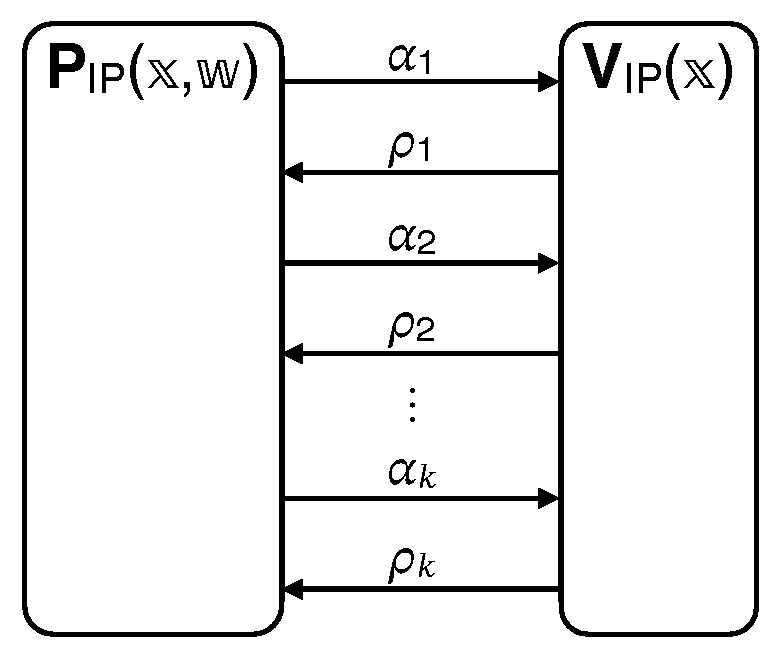
\includegraphics[width=0.5\textwidth]{\FigureFolder/ip-diagram}
\caption{Diagram of an IP.}
\label{figure:ip-diagram}
\end{figure}

The tuple $\IPSymbol=\IPSystem$ is an IP for a relation $\Relation$ with \emph{(perfect) completeness} and \emph{soundness error $\IPSoundnessError$} if it satisfies the two properties stated below.

\begin{definition}
\label{definition:ip-completeness}
$\IPSymbol=\IPSystem$ for a relation $\Relation$ has \defemph{perfect completeness} if for every $(\Instance,\Witness) \in \Relation$
\begin{equation*}
\Pr[
\IPInteract{\IPProver(\Instance,\Witness)}{\IPVerifier(\Instance)}=1
]
=1
\enspace.
\end{equation*}
\end{definition}

\begin{definition}
\label{definition:ip-soundness}
$\IPSymbol=\IPSystem$ for a relation $\Relation$ has \defemph{soundness error $\IPSoundnessError$} if for every $\Instance \notin \GetLanguage{\Relation}$ and malicious IP prover $\IPMaliciousProver$
\begin{equation*}
\Pr[
\IPInteract{\IPMaliciousProver}{\IPVerifier(\Instance)}=1
]
\leq
\IPSoundnessError(\Instance)
\enspace.
\end{equation*}
We additionally define $\IPSoundnessError(\InstanceSize) \DefineEqual \MaxSoundness{\IPSoundnessError(\Instance)}$.
\end{definition}

Above, given two interactive algorithms $A$ and $B$, we use the notation $\IPInteract{A}{B}$ to indicate the random variable that equals the output of $B$ after interacting with $A$, and where the probability is taken over any randomness used by $A$ or $B$.

See \Cref{figure:ip-diagram} for a diagram.

\parhead{Efficiency measures}
We are interested in several efficiency measures of an IP.
\begin{itemize}

  \item \emph{Round complexity}, denoted $\IPRoundComplexity$, is the number of back-and-forth interactions between the IP prover and the IP verifier. Each round contains (at most) two messages: an IP prover message and an IP verifier message. If we wish to be more precise in describing the interaction (e.g., when an IP has small round complexity), we may instead specify the number of \emph{messages} and whether the IP prover or IP verifier sends the first message in the interaction.

  \item \emph{Communication complexity} refers to the total number of bits exchanged between the IP prover and IP verifier. In more detail, for every $\RoundIndex \in [\IPRoundComplexity]$, we denote by $\IPPToVComplexity_{\RoundIndex}$ and $\IPVToPComplexity_{\RoundIndex}$ the size of the $\RoundIndex$-th IP prover message and the $\RoundIndex$-th IP verifier message. Therefore the size of the prover-to-verifier transcript is $\IPPToVComplexity = \sum_{\RoundIndex \in [\IPRoundComplexity]} \IPPToVComplexity_{\RoundIndex}$ and the size of the verifier-to-prover transcript is $\IPVToPComplexity = \sum_{\RoundIndex \in [\IPRoundComplexity]} \IPVToPComplexity_{\RoundIndex}$. In particular, the communication complexity is $\IPPToVComplexity+\IPVToPComplexity$.

  \item \emph{Prover time and verifier time}, denoted $\IPProverTime$ and $\IPVerifierTime$, are the running times of the IP prover and the IP verifier (across the whole interaction).

\end{itemize}
The above efficiency measures may be functions of the given instance $\Instance$ (and possibly other parameters associated to the construction of an IP).

\parhead{Public-coin IPs}
In this book we only consider IPs that are \emph{public-coin}, which is a property of the IP verifier $\IPVerifier$.

\begin{definition}
\label{definition:ip-public-coin}
$\IPSymbol=\IPSystem$ is \defemph{public-coin} if every message $\IPVerifierRandomMessage_{\RoundIndex}$ sent by the IP verifier $\IPVerifier$ is a random binary string of some prescribed size $\IPRandomnessComplexity_{\RoundIndex}$ (that is statistically independent of everything else); moreover, the IP verifier $\IPVerifier$ has no other randomness. In this case, the decision bit of the IP verifier $\IPVerifier$ is a function only of the instance $\Instance$ and the transcript of interaction $(\IPProverMessage_{1},\IPVerifierRandomMessage_{1},\dots,\IPProverMessage_{\IPRoundComplexity},\IPVerifierRandomMessage_{\IPRoundComplexity})$. We denote this bit by
\begin{equation*}
\IPVerifier\big(\IPVerifierInput\big)
\enspace.
\end{equation*}
\end{definition}

In this case the total randomness complexity is $\IPRandomnessComplexity \DefineEqual \sum_{\RoundIndex \in [\IPRoundComplexity]} \IPRandomnessComplexity_{\RoundIndex}$, and the maximum randomness complexity in any round (which we sometimes use in an analysis) is $\IPMaxRandomnessComplexity \DefineEqual \max_{\RoundIndex \in [\IPRoundComplexity]} \IPRandomnessComplexity_{\RoundIndex}$. Moreover, the verifier-to-prover communication complexity coincides with randomness complexity: for every $\RoundIndex \in [\IPRoundComplexity]$, $\IPVToPComplexity_{\RoundIndex} = \IPRandomnessComplexity_{\RoundIndex}$; and thus $\IPVToPComplexity = \sum_{\RoundIndex \in [\IPRoundComplexity]} \IPVToPComplexity_{\RoundIndex} = \sum_{\RoundIndex \in [\IPRoundComplexity]} \IPRandomnessComplexity_{\RoundIndex} = \IPRandomnessComplexity$.


\parhead{Knowledge soundness}
The soundness notion (\Cref{definition:ip-soundness}) can be strengthened to a knowledge soundness notion, which informally means that whenever an IP prover convinces the IP verifier, then an efficient extractor finds a witness (up to some error). In more detail, we require the existence of a probabilistic algorithm $\IPExtractor$ that works as follows. Fix any instance $\Instance$ and IP prover $\IPMaliciousProver$. The IP prover $\IPMaliciousProver$ and IP verifier $\IPVerifier$ (on input $\Instance$) interact; denote by $\IPTranscript$ the transcript of this interaction and by $b$ the decision bit of the IP verifier $\IPVerifier$. The knowledge extractor $\IPExtractor$ is tasked to find a witness $\Witness$ when given as input the instance $\Instance$, the interaction transcript $\IPTranscript$, and black-box access to the IP prover $\IPMaliciousProver$. This means that the knowledge extractor $\IPExtractor$ is \emph{rewinding}: it can re-run the IP prover $\IPMaliciousProver$ multiple times, possibly with correlated inputs. The knowledge soundness error is an upper bound on the probability that $b=1$ ($\IPMaliciousProver$ convinces $\IPVerifier$) and $(\Instance,\Witness) \notin \Relation$ ($\IPExtractor$ does not find a witness). In general, the knowledge soundness error may be a function of the failure probability of $\IPMaliciousProver$, which we define below.

\begin{definition}
\label{definition:ip-failure-probability}
Let $\IPSymbol=\IPSystem$ be an IP. A deterministic IP prover $\IPMaliciousProver$ has \defemph{failure probability $\ProverFailureProbability{\IPMaliciousProver}$} if for every instance $\Instance$:
\begin{equation*}
\Pr[
\IPInteract{\IPMaliciousProver}{\IPVerifier(\Instance)}=0
]
\leq \ProverFailureProbability{\IPMaliciousProver}(\Instance)
\enspace.
\end{equation*}
\end{definition}

\begin{definition}
\label{definition:ip-knowledge-soundness}
$\IPSymbol=\IPSystem$ for a relation $\Relation$ has \defemph{rewinding knowledge soundness error $\IPKnowledgeError$ with extraction time $\IPKnowledgeTime$} if there exists a probabilistic algorithm $\IPExtractor$ (the \emph{extractor}) such that for every instance $\Instance$ and deterministic IP prover $\IPMaliciousProver$ with running time $\ProverRunningTime{\IPMaliciousProver}$ the following holds:
\begin{equation*}
\Pr\left[
\begin{array}{l}
(\Instance,\Witness) \notin \Relation \\
\land\;\DecisionBit=1
\end{array}
\GivenExperiment
\StateExperiment{
\DecisionBit \xleftarrow{\IPTranscript} \IPInteract{\IPMaliciousProver}{\IPVerifier(\Instance)} \\
\Witness \gets \IPExtractor(\Instance,\IPTuple{\IPProverMessage},\IPTuple{\IPVerifierRandomMessage},\BlackBox{\IPMaliciousProver})
}
\right]
\leq
\IPKnowledgeError(\Instance,\ProverFailureProbability{\IPMaliciousProver}(\Instance))
\enspace.
\end{equation*}
Moreover, $\IPExtractor(\Instance,\IPTuple{\IPProverMessage},\IPTuple{\IPVerifierRandomMessage},\BlackBox{\IPMaliciousProver})$ runs in expected time $\IPKnowledgeTime(\Instance,\ProverFailureProbability{\IPMaliciousProver}(\Instance),\ProverRunningTime{\IPMaliciousProver}(\Instance))$. We additionally define
\begin{align*}
\IPKnowledgeError(\InstanceSize,\ProverFailureProbability{\IPMaliciousProver}) &\DefineEqual \MaxKnowledge{\IPKnowledgeError(\Instance,\ProverFailureProbability{\IPMaliciousProver}(\Instance))}
\enspace,\quad\text{and} \\
\IPKnowledgeTime(\InstanceSize,\ProverFailureProbability{\IPMaliciousProver},\ProverRunningTime{\IPMaliciousProver}) &\DefineEqual \MaxKnowledge{\IPKnowledgeTime(\Instance,\ProverFailureProbability{\IPMaliciousProver}(\Instance),\ProverRunningTime{\IPMaliciousProver}(\Instance))}
\enspace.
\end{align*}
\end{definition}

If $\IPSymbol=\IPSystem$ has knowledge soundness error $\IPKnowledgeError$ (with any extraction time $\IPKnowledgeTime$) then it has soundness error $\IPSoundnessError$ such that $\IPSoundnessError(\Instance) \leq \min_{\ProverFailureProbability{} \in [0,1]} \IPKnowledgeError(\Instance,\ProverFailureProbability{})$: if $\Instance \notin \GetLanguage{\Relation}$ then the extractor cannot output a witness $\Witness$ such that $(\Instance,\Witness) \in \Relation$ (as none exists), in which case the event bounded by the knowledge soundness condition equals the event bounded by the soundness condition.

A notable special case of \Cref{definition:ip-knowledge-soundness} is \emph{straightline extraction}: $\IPExtractor$ is a polynomial-time deterministic algorithm that receives as input the instance $\Instance$ and IP prover messages $\IPTuple{\IPProverMessage}$ (but not the IP verifier messages $\IPTuple{\IPVerifierRandomMessage}$ or access to $\IPMaliciousProver$).


\parhead{Zero knowledge}
An IP is \emph{zero knowledge} if the IP prover, when interacting with the IP verifier, reveals no information beyond the fact that the proved statement is true. If the IP verifier is allowed to behave arbitrarily, then the property is called \emph{malicious-verifier} zero knowledge; otherwise, if the IP verifier must follow the honest strategy, then the property is called \emph{honest-verifier} zero knowledge. This latter (and weaker) property suffices for the applications that we consider, and so our definitions focus on that property only. The formal definition consists of two steps:
\begin{inparaenum}[(a)]
  \item we formalize the \emph{view} of the IP verifier, which is all the information that the IP verifier learns by interacting with the IP prover;
  \item we say that the interactive proof is zero knowledge if the view of the IP verifier can be (approximately) simulated by a polynomial-time probabilistic algorithm, known as the \emph{simulator}.
\end{inparaenum}
The intuition here is that anything that is computable efficiently with randomness is \DoQuote{for free}, and so does not count as revealed knowledge. Crucially, the property is only required for instance-witness pairs in the relation, and the simulator is only given as input the instance (but not the witness).

\begin{definition}
\label{definition:ip-view}
The IP verifier's \defemph{view} in $\IPSymbol=\IPSystem$ on the instance-witness pair $(\Instance,\Witness)$, denoted $\IPView{\IPProver}{\IPVerifier}{\Instance}{\Witness}$, is the random variable $\IPSampledView$ where:
\begin{itemize}[nolistsep]
  \item $\IPVerifierRandomness$ is a random choice of randomness for the IP verifier $\IPVerifier$; and
  \item $\IPTuple{\IPProverMessage}$ are the prover messages received in an interaction between $\IPProver(\Instance,\Witness)$ and $\IPVerifier(\Instance,\IPVerifierRandomness)$.
\end{itemize}
Note that the honest IP prover $\IPProver(\Instance,\Witness)$ may use its own private randomness (and is not part of the IP verifier's view). If the IP is public-coin then the view shows each round's randomness: $\IPPublicSampledView$.
\end{definition}

\begin{definition}
\label{definition:ip-hvzk}
$\IPSymbol=\IPSystem$ for a relation $\Relation$ has \defemph{honest-verifier zero-knowledge error $\IPZKError$} if there exists a polynomial-time probabilistic algorithm $\IPSimulator$ such that for every instance-witness pair $(\Instance,\Witness) \in \Relation$ the following random variables are $\IPZKError(\Instance)$-close in statistical distance:
\begin{equation*}
\IPView{\IPProver}{\IPVerifier}{\Instance}{\Witness}
\TextAndInMath
\IPSimulator(\Instance)
\enspace.
\end{equation*}
We additionally define $\IPZKError(\InstanceSize) \DefineEqual \MaxZK{\IPZKError(\Instance)}$.
\end{definition}

%%%%%%%%%%%%%%%%%%%%%%%%%%%%%%%%%%%%%%%%%%%%%%%%%%%%%%%%%%%%%%%%%%%%%%%%%%%%%%%
%%%%%%%%%%%%%%%%%%%%%%%%%%%%%%%%%%%%%%%%%%%%%%%%%%%%%%%%%%%%%%%%%%%%%%%%%%%%%%%
%%%%%%%%%%%%%%%%%%%%%%%%%%%%%%%%%%%%%%%%%%%%%%%%%%%%%%%%%%%%%%%%%%%%%%%%%%%%%%%
\section{State restoration}
\label{section:fs-sr-attacks}

We describe \emph{state-restoration soundness}, a notion of soundness for public-coin IPs. This notion requires security against a more powerful class of malicious provers called \emph{state-restoration provers}.

In \Cref{section:fs-sr-definition} we define state-restoration soundness for IPs. In \Cref{section:fs-sr-comparison} we compare state-restoration soundness and standard soundness for IPs.

The security of a non-interactive argument obtained from a given IP via the Fiat--Shamir transformation is characterized by the state-restoration soundness of the IP, as we discuss in \Cref{chapter:slow-fs-for-ip}. However, in stark contrast to the case of state-restoration soundness for SPs (discussed in \Cref{chapter:fs-for-sp-sr}), good standard soundness for an IP does not, in general, imply good state-restoration soundness. (An IP can have small standard soundness error but huge state-restoration soundness error; see \Cref{remark:sr-tightness-of-upper-bound}.) Therefore, to ensure security of the Fiat--Shamir transformation, one must assume that the given IP has small state-restoration soundness error.

Small state-restoration soundness error is implied by natural strong notions of soundness, such as special soundness (see \Cref{chapter:special-soundness}) and round-by-round soundness (see \Cref{chapter:rbr-soundness}).

Analogous considerations hold for state-restoration \emph{knowledge} soundness versus standard \emph{knowledge} soundness.

%%%%%%%%%%%%%%%%%%%%%%%%%%%%%%%%%%%%%%%%%%%%%%%%%%%%%%%%%%%%%%%%%%%%%%%%%%%%%%%
%%%%%%%%%%%%%%%%%%%%%%%%%%%%%%%%%%%%%%%%%%%%%%%%%%%%%%%%%%%%%%%%%%%%%%%%%%%%%%%
\subsection{Definition}
\label{section:fs-sr-definition}

The standard notion of soundness for an IP considers the setting where a malicious IP prover attempts to convince the IP verifier in a single interaction (see \Cref{definition:ip-soundness}): in each round the malicious IP prover sends a message and the IP verifier responds with some randomness, and at the end of the interaction the IP verifier accepts or rejects based on (the instance and) the transcript of interaction. In contrast, state-restoration soundness considers the setting where a malicious IP prover attempts to convince the IP verifier multiple times across related interactions, and the malicious IP prover wins if it finds an interaction that convinces the IP verifier.

In more detail, we consider an \emph{IP state-restoration game} that informally works as follows. The game samples $\IPRoundComplexity$ random functions to be used as IP verifier randomness: for every $\RoundIndex \in [\IPRoundComplexity]$, the game samples a random function $\SRRandomness_{\RoundIndex} \in \RODistribution{\IPRandomnessComplexity_{\RoundIndex}}$ to choose IP verifier randomness corresponding to the $\RoundIndex$-th round. In this game the goal of the malicious IP prover is to output an instance $\Instance$, IP prover messages $(\IPProverMessage_{1},\dots,\IPProverMessage_{\IPRoundComplexity})$, and salts $(\SRSaltString_{1},\dots,\SRSaltString_{\IPRoundComplexity})$ that convince the IP verifier according to the following condition:
\begin{equation*}
\IPVerifier\big(\IPVerifierInput\big)=1
\quad
\text{where}
\quad
\IPVerifierRandomMessage_{\RoundIndex} \DefineEqual \SRRandomness_{\RoundIndex}\IPSRGameStateEntry{\RoundIndex}
\enspace.
\end{equation*}
Each salt $\SRSaltString_{\RoundIndex}$ is a string of $\SRSaltSize$ bits, for some salt parameter $\SRSaltSize \in \Naturals$.

The malicious IP prover has a budget of $\SRBudget \in \Naturals$ moves to invest in choosing its output. A move consists of outputting a tuple $\IPSRGameStateEntry{\RoundIndex}$ (possibly unrelated to the eventual output), and the game responds with the randomness $\IPVerifierRandomMessage_{\RoundIndex} \DefineEqual \SRRandomness_{\RoundIndex}\IPSRGameStateEntry{\RoundIndex}$.

On one extreme, if the malicious IP prover makes no moves then it has no information about the random functions $\IPTuple{\SRRandomness}$. This means that it chooses an output $\IPSRGameStateEntry{\IPRoundComplexity}$ without seeing any IP verifier random messages. This is a poor way to play the game.

The malicious IP prover can at minimum recreate a single interaction with the IP verifier: output a move $(\Instance,(\IPProverMessage_{1}),(\SRSaltString_{1}))$ to obtain, as a response from the game, the IP verifier challenge $\IPVerifierRandomMessage_{1} \DefineEqual \SRRandomness_{1}(\Instance,(\IPProverMessage_{1}),(\SRSaltString_{1}))$; and then, for each $\RoundIndex \in \{2,\dots,\IPRoundComplexity\}$, output a move $\IPSRGameStateEntry{\RoundIndex}$ based on the prior randomness $\IPVerifierRandomMessage_{1},\dots,\IPVerifierRandomMessage_{\RoundIndex-1}$ and then obtain, as a response from the game, the next round randomness $\IPVerifierRandomMessage_{\RoundIndex} \DefineEqual \SRRandomness_{\RoundIndex}\IPSRGameStateEntry{\RoundIndex}$. This enables the malicious IP prover to win with probability that is at least that of winning in a single interaction with the IP verifier.

However, the malicious IP prover can do more than this: the malicious IP prover can use moves to see multiple \DoQuote{random continuations} of an interaction with the IP verifier. For example, the malicious IP prover can first output a move $(\Instance,(\IPProverMessage_{1}),(\SRSaltString_{1}))$ to obtain the IP verifier challenge $\IPVerifierRandomMessage_{1} \DefineEqual \SRRandomness_{1}(\Instance,(\IPProverMessage_{1}),(\SRSaltString_{1}))$, and subsequently explore two different extensions of this transcript: output the moves $(\Instance,(\IPProverMessage_{1},\IPProverMessage_{2}),(\SRSaltString_{1},\SRSaltString_{2}))$ and $(\Instance,(\IPProverMessage_{1},\IPProverMessage_{2}'),(\SRSaltString_{1},\SRSaltString_{2}))$ for two different IP prover messages $\IPProverMessage_{2}$ and $\IPProverMessage_{2}'$ in order to obtain two different IP verifier challenges $\IPVerifierRandomMessage_{2}$ and $\IPVerifierRandomMessage_{2}'$. And so on.

The salt parameter $\SRSaltSize$ limits how many times the malicious IP prover can extend the same partial transcript. For example, the malicious IP prover can see at most $2^{\SRSaltSize}$ different choices of $\IPVerifierRandomMessage_{1}$ for the same instance $\Instance$ and IP prover message $\IPProverMessage_{1}$. (Each $\SRSaltSize$-bit salt leads to a fresh randomness choice.)

\begin{definition}
\label{definition:ip-state-restoration-game}
The \defemph{IP state-restoration game} for $\IPSymbol=\IPSystem$ with salt size $\SRSaltSize \in \Naturals$, functions $\SRRandomness = \IPTuple{\SRRandomness} \in \RODistribution{\IPTuple{\IPRandomnessComplexity}}$, and IP state-restoration prover $\IPMaliciousSRProver$ is defined below.
\begin{itemize}[noitemsep]
\item[] $\IPStateRestorationGame{\SRSaltSize}{\SRRandomness}{\IPMaliciousSRProver}$:
\begin{enumerate}[nolistsep]
  \item Repeat the following until $\IPMaliciousSRProver$ decides to exit the loop.
  \begin{enumerate}[nolistsep]
    \item $\IPMaliciousSRProver$ outputs $\IPSRGameStateEntry{\RoundIndex}$, where $\Instance$ is an instance, $(\IPProverMessage_{1},\dots,\IPProverMessage_{\RoundIndex})$ are IP prover messages, and $(\SRSaltString_{1},\dots,\SRSaltString_{\RoundIndex})$ are salt strings in $\Bits^{\SRSaltSize}$.
    \item Set $\IPVerifierRandomMessage_{\RoundIndex} \DefineEqual \SRRandomness_{\RoundIndex}\IPSRGameStateEntry{\RoundIndex}$.
    \item Send $\IPVerifierRandomMessage_{\RoundIndex}$ to $\IPMaliciousSRProver$.
  \end{enumerate}
  \item $\IPMaliciousSRProver$ outputs $\IPSRGameStateEntry{\IPRoundComplexity}$, where $\Instance$ is an instance, $(\IPProverMessage_{1},\dots,\IPProverMessage_{\IPRoundComplexity})$ are IP prover messages, and $(\SRSaltString_{1},\dots,\SRSaltString_{\IPRoundComplexity})$ are salt strings in $\Bits^{\SRSaltSize}$.
    \item For every $\RoundIndex \in [\IPRoundComplexity]$, set $\IPVerifierRandomMessage_{\RoundIndex} \DefineEqual \SRRandomness_{\RoundIndex}\IPSRGameStateEntry{\RoundIndex}$.
  \item Output $\IPSROutput$.
\end{enumerate}
\end{itemize}
We denote by $\SRTrace$ the list of move-response pairs of the form $(\IPSRGameStateEntry{\RoundIndex},\IPVerifierRandomMessage_{\RoundIndex})$ performed in the loop. We show $\SRTrace$ in an execution of the IP state-restoration game using the following notation:
\begin{equation*}
\IPSROutput \xleftarrow{\SRTrace} \IPStateRestorationGame{\SRSaltSize}{\SRRandomness}{\IPMaliciousSRProver}
\enspace.
\end{equation*}
We say that $\IPMaliciousSRProver$ is \defemph{$\SRBudget$-move} if $\IPMaliciousSRProver$ exits the loop after at most $\SRBudget$ iterations.
\end{definition}

The above game directly leads to the notion of state-restoration soundness error: it is an upper bound on the probability that any IP prover in the IP state-restoration game can find an instance not in the language and an accepting transcript for it.

\begin{definition}
\label{definition:ip-state-restoration-soundness}
$\IPSymbol=\IPSystem$ has \defemph{state-restoration soundness error $\IPSRSoundnessError$} if for every salt size $\SRSaltSize \in \Naturals$, move budget $\SRBudget \in \Naturals$, $\SRBudget$-move malicious IP state-restoration prover $\IPMaliciousSRProver$, and instance size bound $\InstanceSize \in \Naturals$:
\begin{equation*}
\Pr\left[
\begin{array}{l}
\SomeSize{\Instance} \leq \InstanceSize \\
\land\;\Instance \notin \GetLanguage{\Relation} \\
\land\;\IPVerifier\big(\IPVerifierInput\big)=1
\end{array}
\GivenExperiment
\StateExperiment{
\SRRandomness = \IPTuple{\SRRandomness} \gets \RODistribution{\IPTuple{\IPRandomnessComplexity}} \\
\LongExecution{\IPSROutput}{\IPStateRestorationGame{\SRSaltSize}{\SRRandomness}{\IPMaliciousSRProver}}
}
\right]
\leq \IPSRSoundnessError(\SRSaltSize,\SRBudget,\InstanceSize)
\enspace.
\end{equation*}
\end{definition}

We also define the notion of state-restoration \emph{knowledge soundness} error: it is an upper bound on the probability that any IP prover in the IP state-restoration game can find an instance and an accepting transcript for it such that an extractor algorithm cannot find a witness for the instance (given the relevant information about the malicious prover and its moves in the game).

In more detail, we consider two flavors of state-restoration knowledge soundness: \textbf{straightline} knowledge soundness, and a relaxation known as \textbf{rewinding} knowledge soundness.\footnote{Many IPs of interest satisfy the relaxed notion of rewinding knowledge soundness rather than the stronger notion of straightline knowledge soundness. Nevertheless, we consider both for two reasons. First, the straightline flavor is simpler to understand than the rewinding flavor, so it plays a meaningful pedagogical unit. Second, in \Cref{section:bcs-knowledge-soundness} we rely on (a relaxation of) the straightline variant as an intermediate notion when proving the knowledge soundness of \Cref{construction:bcs-transformation} as a composition of two transformations.}

The straightline variant of state-restoration knowledge soundness considers a (deterministic) knowledge extractor $\IPSRExtractor$ that is tasked with finding a witness $\Witness$ while given the final output $\IPSRGameStateEntry{\IPRoundComplexity}$ of the state-restoration prover $\IPMaliciousSRProver$ and its move-response trace $\SRTrace$. The knowledge extractor $\IPSRExtractor$ does not receive the randomness $\IPTuple{\IPVerifierRandomMessage}$ used by the IP verifier.

\begin{definition}
\label{definition:ip-state-restoration-knowledge-straightline}
$\IPSymbol=\IPSystem$ has \defemph{straightline state-restoration knowledge soundness error $\IPSRKnowledgeError$} if there exists a polynomial-time deterministic algorithm $\IPSRExtractor$ (the \emph{extractor}) such that for every salt size $\SRSaltSize \in \Naturals$, move budget $\SRBudget \in \Naturals$, $\SRBudget$-move deterministic IP state-restoration prover $\IPMaliciousSRProver$, and instance size bound $\InstanceSize$:
\begin{equation*}
\Pr\left[
\begin{array}{l}
\SomeSize{\Instance} \leq \InstanceSize \\
\land\;(\Instance,\Witness) \notin \Relation \\
\land\;\IPVerifier\big(\IPVerifierInput\big)=1
\end{array}
\GivenExperiment
\StateExperiment{
\SRRandomness = \IPTuple{\SRRandomness} \gets \RODistribution{\IPTuple{\IPRandomnessComplexity}} \\
\LongExecutionOver{\IPSROutput}{\IPStateRestorationGame{\SRSaltSize}{\SRRandomness}{\IPMaliciousSRProver}}{\SRTrace} \\
\Witness \gets \IPSRExtractor(\Instance,\IPTuple{\IPProverMessage},\IPTuple{\SRSaltString},\SRTrace)
}
\right]
\leq \IPSRKnowledgeError(\SRSaltSize,\SRBudget,\InstanceSize)
\enspace.
\end{equation*}
\end{definition}

The rewinding variant of state-restoration knowledge soundness relaxes the prior notion by considering a knowledge extractor that additionally receives the randomness $\IPTuple{\IPVerifierRandomMessage}$ used by the IP verifier and black-box access to the state-restoration prover $\IPMaliciousSRProver$. In this case, the error may additionally depend on the failure probability of $\IPMaliciousSRProver$ (an upper bound on the probability that the final output of $\IPMaliciousSRProver$ does \emph{not} convince the IP verifier). Intuitively, as the failure probability increases, the error of extraction increases.

The motivation to consider the rewinding variant is that there are notable classes of IPs that satisfy this property. For example, in \Cref{chapter:special-soundness}, we discuss how IPs that satisfy \emph{special soundness} also satisfy rewinding state-restoration knowledge soundness.

\begin{definition}
\label{definition:ip-sr-failure-probability}
Let $\IPSymbol=\IPSystem$ be an IP. A deterministic IP state-restoration prover $\IPMaliciousSRProver$ has \defemph{failure probability $\ProverFailureProbability{\IPMaliciousSRProver}$} if for every salt size $\SRSaltSize \in \Naturals$ and instance size bound $\InstanceSize$:
\begin{equation*}
\Pr\left[
\begin{array}{l}
\SomeSize{\Instance} \leq \InstanceSize \\
\land\;\IPVerifier\big(\IPVerifierInput\big)=0
\end{array}
\GivenExperiment
\StateExperiment{
\SRRandomness = \IPTuple{\SRRandomness} \gets \RODistribution{\IPTuple{\IPRandomnessComplexity}} \\
\LongExecution{\IPSROutput}{\IPStateRestorationGame{\SRSaltSize}{\SRRandomness}{\IPMaliciousSRProver}}
}
\right]
\leq \ProverFailureProbability{\IPMaliciousSRProver}(\SRSaltSize,\InstanceSize)
\enspace.
\end{equation*}
\end{definition}

\begin{definition}
\label{definition:ip-state-restoration-knowledge}
$\IPSymbol=\IPSystem$ has \defemph{rewinding state-restoration knowledge soundness error $\IPSRKnowledgeError$ with extraction time $\IPSRKnowledgeTime$} if there exists a probabilistic algorithm $\IPSRExtractor$ (the \emph{extractor}) such that for every salt size $\SRSaltSize \in \Naturals$, move budget $\SRBudget \in \Naturals$, $\SRBudget$-move deterministic IP state-restoration prover $\IPMaliciousSRProver$ with failure probability $\ProverFailureProbability{\IPMaliciousSRProver}$ and running time $\ProverRunningTime{\IPMaliciousSRProver}$, and instance size bound $\InstanceSize$:
\begin{align*}
\Pr&\left[
\begin{array}{l}
\SomeSize{\Instance} \leq \InstanceSize \\
\land\;(\Instance,\Witness) \notin \Relation \\
\land\;\IPVerifier\big(\IPVerifierInput\big)=1
\end{array}
\GivenExperiment
\StateExperiment{
\SRRandomness = \IPTuple{\SRRandomness} \gets \RODistribution{\IPTuple{\IPRandomnessComplexity}} \\
\LongExecutionOver{\IPSROutput}{\IPStateRestorationGame{\SRSaltSize}{\SRRandomness}{\IPMaliciousSRProver}}{\SRTrace} \\
\Witness \gets \IPSRExtractor(\Instance,\IPTuple{\IPProverMessage},\SRSaltStrings{\IPRoundComplexity},\IPTuple{\IPVerifierRandomMessage},\SRTrace,\BlackBox{\IPMaliciousSRProver})
}
\right]
\\ & \leq \IPSRKnowledgeError(\SRSaltSize,\SRBudget,\InstanceSize,\ProverFailureProbability{\IPMaliciousSRProver}(\SRSaltSize,\InstanceSize))
\enspace.
\end{align*}
Moreover, $\IPSRExtractor$ runs in expected time $\IPSRKnowledgeTime(\SRSaltSize,\SRBudget,\InstanceSize,\ProverFailureProbability{\IPMaliciousSRProver}(\SRSaltSize,\InstanceSize),\ProverRunningTime{\IPMaliciousSRProver}(\SRSaltSize,\InstanceSize))$ (over the given inputs and internal randomness).
\end{definition}

\begin{remark}[non-adaptive choice of instance]
\label{remarm:sr-non-adaptive-choice-of-instance}
The IP state-restoration soundness and knowledge soundness games naturally restrict to the setting where the instance $\Instance$ is fixed in advance, rather than being chosen by the IP prover $\IPMaliciousSRProver$. Here we consider an adaptive choice of instance $\Instance$ to match the adaptive soundness and knowledge soundness notions that we consider for non-interactive arguments.
\end{remark}

%%%%%%%%%%%%%%%%%%%%%%%%%%%%%%%%%%%%%%%%%%%%%%%%%%%%%%%%%%%%%%%%%%%%%%%%%%%%%%%
%%%%%%%%%%%%%%%%%%%%%%%%%%%%%%%%%%%%%%%%%%%%%%%%%%%%%%%%%%%%%%%%%%%%%%%%%%%%%%%
\subsection{Comparison with standard soundness}
\label{section:fs-sr-comparison}

The lemma below compares state-restoration soundness to (standard) soundness for public-coin IPs. The lower bound tells us that state-restoration soundness error is at least a multiplicative factor of $\Omega(\frac{\SRBudget}{\IPRoundComplexity})$ larger than standard soundness error. But it can be much larger than that, especially if the round complexity $\IPRoundComplexity$ of the IP is large. Both the upper bound and the lower bound in the lemma are right up to small-order terms, as explained in the corresponding remarks below.

\begin{lemma}
\label{lemma:ip-sr-vs-standard}
Let $\IPSymbol=\IPSystem$ be a public-coin IP with round complexity $\IPRoundComplexity$ and soundness error $\IPSoundnessError$. For every $\SRSaltSize,\SRBudget,\InstanceSize \in \Naturals$ with $\SRSaltSize \geq \log \frac{\SRBudget}{\IPRoundComplexity}$, $\IPSymbol$ has state-restoration soundness error $\IPSRSoundnessError$ such that
\begin{equation*}
\floor{\frac{\SRBudget}{\IPRoundComplexity}} \cdot \IPSoundnessError(\InstanceSize)
-
\binom{\floor{\frac{\SRBudget}{\IPRoundComplexity}}}{2} \cdot \IPSoundnessError(\InstanceSize)^{2}
\leq
\IPSRSoundnessError(\SRSaltSize,\SRBudget,\InstanceSize)
\leq
\binom{\SRBudget + \IPRoundComplexity}{\IPRoundComplexity} \cdot \IPSoundnessError(\InstanceSize)
\enspace.
\end{equation*}
\end{lemma}

\begin{proof}[Proof of lower bound]
We show that
\begin{equation*}
\IPSRSoundnessError(\SRSaltSize,\SRBudget,\InstanceSize)
\geq
\floor{\frac{\SRBudget}{\IPRoundComplexity}} \cdot \IPSoundnessError(\InstanceSize)
-
\binom{\floor{\frac{\SRBudget}{\IPRoundComplexity}}}{2} \cdot \IPSoundnessError(\InstanceSize)^{2}
\enspace.
\end{equation*}
We describe a \DoQuote{universal} state-restoration attack. Let $\IPMaliciousProver$ be a malicious IP prover that convinces the IP verifier $\IPVerifier$ with probability exactly $\IPSoundnessError$. Consider the IP state-restoration prover $\IPMaliciousSRProver$ that, in the IP state-restoration game, runs $\IPMaliciousProver$ for $\floor{\frac{\SRBudget}{\IPRoundComplexity}}$ times, each time with a unique salt. (This is possible because $\SRSaltSize \geq \log \frac{\SRBudget}{\IPRoundComplexity}$.) Then $\IPMaliciousSRProver$ outputs an accepting execution, if any exists. Each execution costs $\IPRoundComplexity$ moves, and convinces the IP verifier $\IPVerifier$ with probability $\IPSoundnessError$ (independently of any other executions). By the simple inclusion-exclusion principle (\Cref{lemma:inclusion-exclusion-2}), the probability that at least one execution is accepting is at least the lower bound stated above.
\end{proof}

\begin{remark}[tightness of the lower bound]
\label{remark:sr-tightness-of-lower-bound}
The lower bound above is tight up to small-order terms. In particular, there is a public-coin IP with round complexity $\IPRoundComplexity$, soundness error $\IPSoundnessError$, and state-restoration soundness error $\IPSRSoundnessError$ such that $\IPSRSoundnessError(\SRSaltSize,\SRBudget,\InstanceSize) \leq \SRBudget \cdot \IPSoundnessError(\InstanceSize)$.

Consider the following IP for a trivial language $\Language$: the IP verifier sends $\log 1/\IPSoundnessError$ random bits as its first message, and accepts if and only if all bits are $0$ or $\Instance \in \Language$; pad the rest of the interaction with dummy rounds so to obtain a $\IPRoundComplexity$-round public-coin protocol. The IP verifier accepts instances $\Instance \in \Language$ with probability $1$, and accepts instances $\Instance \notin \Language$ with probability $\IPSoundnessError$. For this public-coin IP, the state-restoration soundness error is at most $\SRBudget \cdot \IPSoundnessError(\InstanceSize)$ (because an IP state-restoration prover has at most $\SRBudget$ attempts to obtain an all-zero message from the IP verifier).
\end{remark}

\begin{proof}[Proof of upper bound]
We show that
\begin{equation*}
\IPSRSoundnessError(\SRSaltSize,\SRBudget,\InstanceSize)
\leq
\binom{\SRBudget + \IPRoundComplexity}{\IPRoundComplexity} \cdot \IPSoundnessError(\InstanceSize)
\enspace.
\end{equation*}
Let $\IPMaliciousSRProver$ be an IP state-restoration prover that wins the IP state-restoration game $\IPStateRestorationGame{\SRSaltSize}{\SRRandomness}{\IPMaliciousSRProver}$ with probability $\delta$. Assume, without loss of generality, that $\IPMaliciousSRProver$ does not make duplicate moves. Moreover, assume that the final output $\IPSRGameStateEntry{\IOPRoundComplexity}$ of $\IPMaliciousSRProver$ is such that the moves $\IPSRGameStateEntry{\RoundIndex}$ for all $\RoundIndex \in [\IOPRoundComplexity]$ have been previously performed; this can be ensured by increasing the move budget from $\SRBudget$ to $\SRBudget + \IOPRoundComplexity$. We construct a malicious IP prover $\IPMaliciousProver$ that convinces the IP verifier $\IPVerifier$ with probability at least $\binom{\SRBudget + \IPRoundComplexity}{\IPRoundComplexity}^{-1} \cdot \delta$ (without any state restoration).
\begin{itemize}[noitemsep]
\item[] $\IPMaliciousProver$:
\begin{enumerate}[nolistsep]
  \item Sample a random subset $S \subseteq [\SRBudget + \IPRoundComplexity]$ of cardinality $\IPRoundComplexity$.
  \item For every $\RoundIndex \in [\IPRoundComplexity]$, denote by $S[\RoundIndex]$ the $\RoundIndex$-th smallest value in $S$.
  \item For every $\RoundIndex \in [\IPRoundComplexity]$, lazily sample an oracle $\LazySub{\SRRandomness}{\RoundIndex} \gets \RODistribution{\IPRandomnessComplexity_{\RoundIndex}}$.
  \item Simulate an execution of the IP state-restoration game with $\IPMaliciousSRProver$, where the $j$-th move is answered as follows:
  \begin{enumerate}[nolistsep]
    \item Let $\RoundIndex \in [\IPRoundComplexity]$ be such that the move has the form $\IPSRGameStateEntry{\RoundIndex}$.
    \item If $j = S[\RoundIndex]$: send the prover message $\IPProverMessage_{\RoundIndex}$ to the IP verifier, receive the random message $\IPVerifierRandomMessage_{\RoundIndex}$, and answer the move with $\IPVerifierRandomMessage_{\RoundIndex}$.
    \item If $j \neq S[\RoundIndex]$: answer the move with $\LazySub{\SRRandomness}{\RoundIndex}\IPSRGameStateEntry{\RoundIndex}$.
  \end{enumerate}
\end{enumerate}
\end{itemize}

The IP state-restoration game allows $\IPMaliciousSRProver$ to attempt to convince the IP verifier across multiple related interactions, with each round of the game corresponds to a random extension for a chosen partial transcript (that might or might not exist as a previous move). When $\IPMaliciousSRProver$ ultimately chooses a transcript of interaction, we can associate distinct indices $i_{1},\dots,i_{\IPRoundComplexity} \subseteq [\SRBudget+\IPRoundComplexity]$ such that the randomness used by the IP verifier in round $j$ is the randomness returned to $\IPMaliciousSRProver$ in round $i_{j}$ of the game. In other words, the transcript of interaction chosen by $\IPMaliciousSRProver$ appears as a subset of its $\SRBudget+\IPRoundComplexity$ moves. Hence we can construct an IP prover $\IPMaliciousProver$ from $\IPMaliciousSRProver$ by guessing this subset, playing against the real IP verifier on this subset, and simulating the rest of the game.
\end{proof}

\begin{remark}[tightness of the upper bound]
\label{remark:sr-tightness-of-upper-bound}
The upper bound above is tight up to small-order terms. In particular, there is a public-coin IP with round complexity $\IPRoundComplexity$, soundness error $\IPSoundnessError$, and state-restoration soundness error $\IPSRSoundnessError$ such that $\IPSRSoundnessError(\SRSaltSize,\SRBudget,\InstanceSize) \geq \binom{\SRBudget/6}{\IPRoundComplexity} \cdot \IPSoundnessError(\InstanceSize)$.

Let $\Language$ be a language decidable in polynomial time, and consider the following $\IPRoundComplexity$-round IP for $\Language$. The IP verifier sends $\ell \DefineEqual \frac{\log 1/\IPSoundnessError}{\IPRoundComplexity}$ random bits in each round, and accepts an instance $\Instance$ if and only if $\Instance \in \Language$ (by using the language's decider) or all random bits in every round are zero. The soundness error of this IP is $\IPSoundnessError$.

Consider an IP state-restoration prover that makes $\SRBudget/\IPRoundComplexity$ moves per round, attempting to obtain random bits for this round that are all zero. If $\SRBudget/\IPRoundComplexity \geq 2^{\ell}$ then this attack succeeds with probability one. If instead $\SRBudget/\IPRoundComplexity < 2^{\ell}$, then we can use the inclusion-exclusion principle (\Cref{lemma:inclusion-exclusion-2}). For any $i \in [\SRBudget/\IPRoundComplexity]$, let $\Event_{i}$ be the event that the $i$-th move is answered with $\ell$ zeros. Then, the probability of succeeding in a particular round is at least
\begin{align*}
\Pr[\idxlor{i \in [\SRBudget/\IPRoundComplexity]} \Event_{i}]
& \geq
\sum_{i \in [\SRBudget/\IPRoundComplexity]} \Pr[\Event_{i}] -
\sum_{\substack{i,j \in [\SRBudget/\IPRoundComplexity] \\ \text{with } i \neq j}} \Pr[\Event_{i} \land \Event_{j}]
\\ & =
\frac{\SRBudget}{\IPRoundComplexity} \cdot \frac{1}{2^{\ell}} - \binom{\SRBudget/\IPRoundComplexity}{2} \cdot \frac{1}{2^{2\ell}}
\\ & \geq
\frac{\SRBudget}{\IPRoundComplexity} \cdot \frac{1}{2^{\ell}} - \frac{(\SRBudget/\IPRoundComplexity)^2}{2} \cdot \frac{1}{2^{2\ell}}
\\ & \geq
\frac{\SRBudget}{\IPRoundComplexity} \cdot \frac{1}{2^{\ell}} - \frac{\SRBudget/\IPRoundComplexity}{2} \cdot \frac{1}{2^{\ell}} \EquationComment{since $\SRBudget/\IPRoundComplexity < 2^{\ell}$}
\\ & =
\frac{\SRBudget}{2\IPRoundComplexity} \cdot \frac{1}{2^{\ell}}
\enspace.
\end{align*}
We conclude that
\begin{align*}
\IPSRSoundnessError(\SRSaltSize,\SRBudget,\InstanceSize)
&\geq
\left(\frac{\SRBudget}{2\IPRoundComplexity} \cdot \frac{1}{2^{\ell}} \right)^{\IPRoundComplexity} \\
&\geq
\left(\frac{e \cdot \SRBudget/6}{\IPRoundComplexity}\right)^{\IPRoundComplexity} \cdot \frac{1}{2^{\IPRoundComplexity \cdot \ell}} \EquationComment{since $1/2 > e/6$} \\
&\geq
\binom{\SRBudget/6}{\IPRoundComplexity} \cdot \IPSoundnessError(\InstanceSize)
\enspace. \EquationComment{by \Cref{lemma:binom-approx}}
\end{align*}
\end{remark}







%%%%%%%%%%%%%%%%%%%%%%%%%%%%%%%%%%%%%%%%%%%%%%%%%%%%%%%%%%%%%%%%%%%%%%%%%%%%%%%
%%%%%%%%%%%%%%%%%%%%%%%%%%%%%%%%%%%%%%%%%%%%%%%%%%%%%%%%%%%%%%%%%%%%%%%%%%%%%%%
%%%%%%%%%%%%%%%%%%%%%%%%%%%%%%%%%%%%%%%%%%%%%%%%%%%%%%%%%%%%%%%%%%%%%%%%%%%%%%%
%%%%%%%%%%%%%%%%%%%%%%%%%%%%%%%%%%%%%%%%%%%%%%%%%%%%%%%%%%%%%%%%%%%%%%%%%%%%%%%
\chapter{The Fiat--Shamir transformation for IPs}
\label{chapter:slow-fs-for-ip}

We describe how to transform any public-coin interactive proof (IP) into a corresponding non-interactive argument, via a construction that is known as the \emph{Fiat--Shamir transformation} \cite{FiatS86}.

The key idea of the construction is to use the random oracle to emulate an interaction between the IP prover and IP verifier, and set the argument string to include the IP prover messages of the interaction. This builds on the case of SPs (a special case of public-coin IPs) discussed in \Cref{part:narg-from-sp}. Similarly to the case of SPs, the construction's only goal is to \DoQuote{remove the interaction} and, in particular, results in an argument string that is at least as large as the IP prover-to-verifier communication complexity. Hence the resulting non-interactive argument is not succinct.

\parhead{Organization}
In \Cref{section:slow-fs-for-ip} we describe the construction. In \Cref{section:slow-fs-attack-sr} we provide a lower bound on the soundness error. In \Cref{section:slow-fs-reduction} we provide an upper bound on the soundness error. In \Cref{section:slow-fs-knowledge-soundness} we provide an upper bound on the knowledge soundness error.

%%%%%%%%%%%%%%%%%%%%%%%%%%%%%%%%%%%%%%%%%%%%%%%%%%%%%%%%%%%%%%%%%%%%%%%%%%%%%%%
%%%%%%%%%%%%%%%%%%%%%%%%%%%%%%%%%%%%%%%%%%%%%%%%%%%%%%%%%%%%%%%%%%%%%%%%%%%%%%%
%%%%%%%%%%%%%%%%%%%%%%%%%%%%%%%%%%%%%%%%%%%%%%%%%%%%%%%%%%%%%%%%%%%%%%%%%%%%%%%
\section{Construction}
\label{section:slow-fs-for-ip}

We describe how to transform any public-coin IP into a non-interactive argument. The high-level idea is that the argument prover can emulate an interaction of the IP prover and the IP verifier by using the random oracle to derive the IP verifier challenges, and subsequently send an argument string that contains the IP prover messages corresponding to this interaction (which the argument verifier can check by re-deriving the IP verifier challenges). Turning this high-level idea into a secure construction involves delicate technical details, which we discuss below.

\parhead{Intuition}
Let $\IPSymbol=\IPSystem$ be a public-coin IP with round complexity $\IPRoundComplexity$. We wish to construct a non-interactive argument $\NARGSymbol=\ARGSystem$ where the argument prover $\ARGProver$ uses the random oracle to emulate an interaction between the IP prover and IP verifier, and the argument verifier $\ARGVerifier$ uses the random oracle to reconstruct this interaction and uses the IP verifier to check the interaction.

The argument prover $\ARGProver$ derives the first IP verifier challenge $\IPVerifierRandomMessage_{1}$ analogously to the case of an SP in \Cref{construction:fs-for-sp}: $\ARGProver$ uses the IP prover $\IPProver$ to compute the first IP prover message $\IPProverMessage_{1}$, and then sets the first IP verifier challenge to be $\IPVerifierRandomMessage_{1} \DefineEqual \ROFunction(\Instance,\IPProverMessage_{1})$.\footnote{We discuss the adjustment of output sizes to match the length of IP verifier challenges later on.} Recall from \Cref{section:fs-lack-of-adaptive-soundness} that the instance $\Instance$ appears in the query $(\Instance,\IPProverMessage_{1})$ in order to ensure adaptive security, intuitively ensuring that a malicious argument prover cannot choose the instance $\Instance$ after seeing the query answer $\IPVerifierRandomMessage_{1}$.

But how should the argument prover $\ARGProver$ derive subsequent IP verifier challenges $\IPVerifierRandomMessage_{\RoundIndex}$ with $\RoundIndex > 1$? (This question did not arise in the case of an SP, where there is a single IP verifier challenge.)

An idea is to set $\IPVerifierRandomMessage_{\RoundIndex} \DefineEqual \ROFunction(\Instance,\IPProverMessage_{\RoundIndex})$ where $\IPProverMessage_{\RoundIndex}$ is the $\RoundIndex$-th IP prover message.

However this does not \DoQuote{enforce} the chronological order of interaction: a malicious argument prover could compute the second IP verifier challenge $\IPVerifierRandomMessage_{2} \DefineEqual \ROFunction(\Instance,\IPProverMessage_{2})$ for a specially-chosen message $\IPProverMessage_{2}$, and only after that compute the first IP verifier challenge $\IPVerifierRandomMessage_{1} \DefineEqual \ROFunction(\Instance,\IPProverMessage_{1})$ for a specially-chosen message $\IPProverMessage_{1}$ that depends on $\IPVerifierRandomMessage_{2}$, which could lead to an attack against the non-interactive argument. For example, suppose that the IP verifier accepts if and only if $\IPProverMessage_{1} = \IPVerifierRandomMessage_{2}$ (the IP prover first message equals the IP verifier second challenge). While this event occurs with a small probability in an interaction between an IP prover and the IP verifier (because the IP prover sends its first message before the IP verifier second challenge is sampled and sent), a malicious argument prover can make this event occur always if IP verifier challenges are derived as $\IPVerifierRandomMessage_{\RoundIndex} \DefineEqual \ROFunction(\Instance,\IPProverMessage_{\RoundIndex})$.

A natural solution, which we will show is secure, is to derive IP verifier challenges by including \emph{all} IP prover messages so far in the query to the random oracle:
\begin{equation*}
\IPVerifierRandomMessage_{\RoundIndex}
\DefineEqual
\ROFunction(\Instance,\IPProverMessage_{1},\dots,\IPProverMessage_{\RoundIndex})
\enspace.
\end{equation*}
Intuitively, this ensures that the argument prover \DoQuote{commits} to the IP prover messages $\IPProverMessage_{1},\dots,\IPProverMessage_{\RoundIndex}$ before seeing the $\RoundIndex$-th IP verifier challenge $\IPVerifierRandomMessage_{\RoundIndex}$, which chronologically comes after these messages.

\parhead{Additional considerations}
Analogously to the case of SPs in \Cref{construction:fs-for-sp}, deriving IP verifier challenges requires additional care.
\begin{itemize}

\item \emph{Salts.}
Each query to the random oracle should be unpredictable (so that we can prove adaptive zero knowledge), and so each query includes a fresh salt. In more detail, the argument prover includes a random salt $\RandSaltString_{\RoundIndex}$ in the query to derive the $\RoundIndex$-th IP verifier challenge. Again to enforce a precise chronological order, each query additionally includes all prior salts. Overall, for every $\RoundIndex \in [\IPRoundComplexity]$, the query to derive the $\RoundIndex$-th IP verifier challenge is as follows:
\begin{equation*}
\IPVerifierRandomMessage_{\RoundIndex}
\DefineEqual
\ROFunction\SlowFSLaterQuery{\RoundIndex}
\enspace.
\end{equation*}

\item \emph{Output sizes.}
The $\RoundIndex$-th IP verifier challenge consists of $\IPRandomnessComplexity_{\RoundIndex}$ bits, so we use a random oracle $\ROFunction_{\RoundIndex} \in \RODistribution{\IPRandomnessComplexity_{\RoundIndex}}$ to derive this challenge. Overall, given random oracles $\IPTuple{\ROFunction} \in \RODistribution{\IPTuple{\IPRandomnessComplexity}}$, for every $\RoundIndex \in [\IPRoundComplexity]$, the $\RoundIndex$-th IP verifier challenge is derived as follows:
\begin{equation*}
\IPVerifierRandomMessage_{\RoundIndex}
\DefineEqual
\begin{cases}
\ROFunction_{1}\FSFirstQuery
& \text{ if $\RoundIndex=1$} \\
\ROFunction_{\RoundIndex}\SlowFSLaterQuery{\RoundIndex}
& \text{ if $\RoundIndex>1$}
\end{cases}
\enspace.
\end{equation*}

\end{itemize}

\parhead{Final construction}
The above considerations lead to the following construction.

\begin{ImportantConstruction}{\FSonIPText}{slow-fs-for-public-coin-ip}
Let $\IPSymbol=\IPSystem$ be a public-coin IP with round complexity $\IPRoundComplexity$. Let $\SecurityParameter \in \Naturals$ be a security parameter and $\PrivacyParameter \in \Naturals$ be a privacy parameter.

We define $\NARGSymbol \DefineEqual \FSonIPTransformation{\IPSymbol}{\SecurityParameter}{\PrivacyParameter}$ to be the non-interactive argument $\NARGSymbol=\ARGSystem$ constructed as follows. The argument prover $\ARGProver$ receives as input an instance $\Instance$ and witness $\Witness$, and the argument verifier $\ARGVerifier$ receives as input the instance $\Instance$ and an argument string $\ARGString$. Both receive query access to random oracles $\IPTuple{\ROFunction} \in \RODistribution{\IPTuple{\IPRandomnessComplexity}}$; this implies that the oracle configuration $\ARGOracles$ is defined as $\ARGOracles(\SecurityParameter,\InstanceSize) \DefineEqual \IPTuple{\IPRandomnessComplexity}$ (see \Cref{definition:narg-oracle-configuration}).
\begin{itemize}

  \item $\ARGProver^{\ROFunction}(\Instance,\Witness)$:
  \begin{enumerate}[nolistsep]
    \item For $\RoundIndex = 1,\dots,\IPRoundComplexity$:
    \begin{enumerate}[nolistsep]
      \item \label{step:slow-fs-for-general-prover-derivation}
      Compute the $\RoundIndex$-th message (and auxiliary state) of the IP prover:
      \begin{equation*}
      (\IPProverMessage_{\RoundIndex},\IPAuxiliaryState_{\RoundIndex})
      \DefineEqual
      \begin{cases}
      \IPProver(\Instance,\Witness)
      & \text{ if $\RoundIndex=1$} \\
      \IPProver(\IPAuxiliaryState_{\RoundIndex-1},\IPVerifierRandomMessage_{\RoundIndex-1})
      & \text{ if $\RoundIndex>1$}
      \end{cases}
      \enspace.
      \end{equation*}
      \item Sample a random salt $\RandSaltString_{\RoundIndex} \in \Bits^{\RandSaltSize}$.
      \item \label{step:slow-fs-for-general-challenge-derivation}
      Derive the $\RoundIndex$-th random message of the IP verifier:
      \begin{equation*}
      \IPVerifierRandomMessage_{\RoundIndex}
      \DefineEqual
      \begin{cases}
      \ROFunction_{1}\FSFirstQuery
      & \text{ if $\RoundIndex=1$} \\
      \ROFunction_{\RoundIndex}\SlowFSLaterQuery{\RoundIndex}
      & \text{ if $\RoundIndex>1$}
      \end{cases}
      \enspace.
      \end{equation*}
    \end{enumerate}
    \item Output the argument string $\ARGString \DefineEqual \FSARGString$.
  \end{enumerate}

  \item $\ARGVerifier^{\ROFunction}(\Instance,\ARGString)$:
  \begin{enumerate}[nolistsep]
    \item Parse the argument string $\ARGString$ as a tuple $\FSARGString$.
    \item For $\RoundIndex = 1,\dots,\IPRoundComplexity$:
    \begin{enumerate}[nolistsep]
      \item derive the $\RoundIndex$-th IP verifier message $\IPVerifierRandomMessage_{\RoundIndex}$ as in \Cref{step:slow-fs-for-general-challenge-derivation} of the argument prover $\ARGProver$.
    \end{enumerate}
    \item Check that the IP verifier accepts: $\IPVerifier\big(\IPVerifierInput\big)=1$.
  \end{enumerate}

\end{itemize}
\end{ImportantConstruction}

\begin{figure}[htp!]
\centering
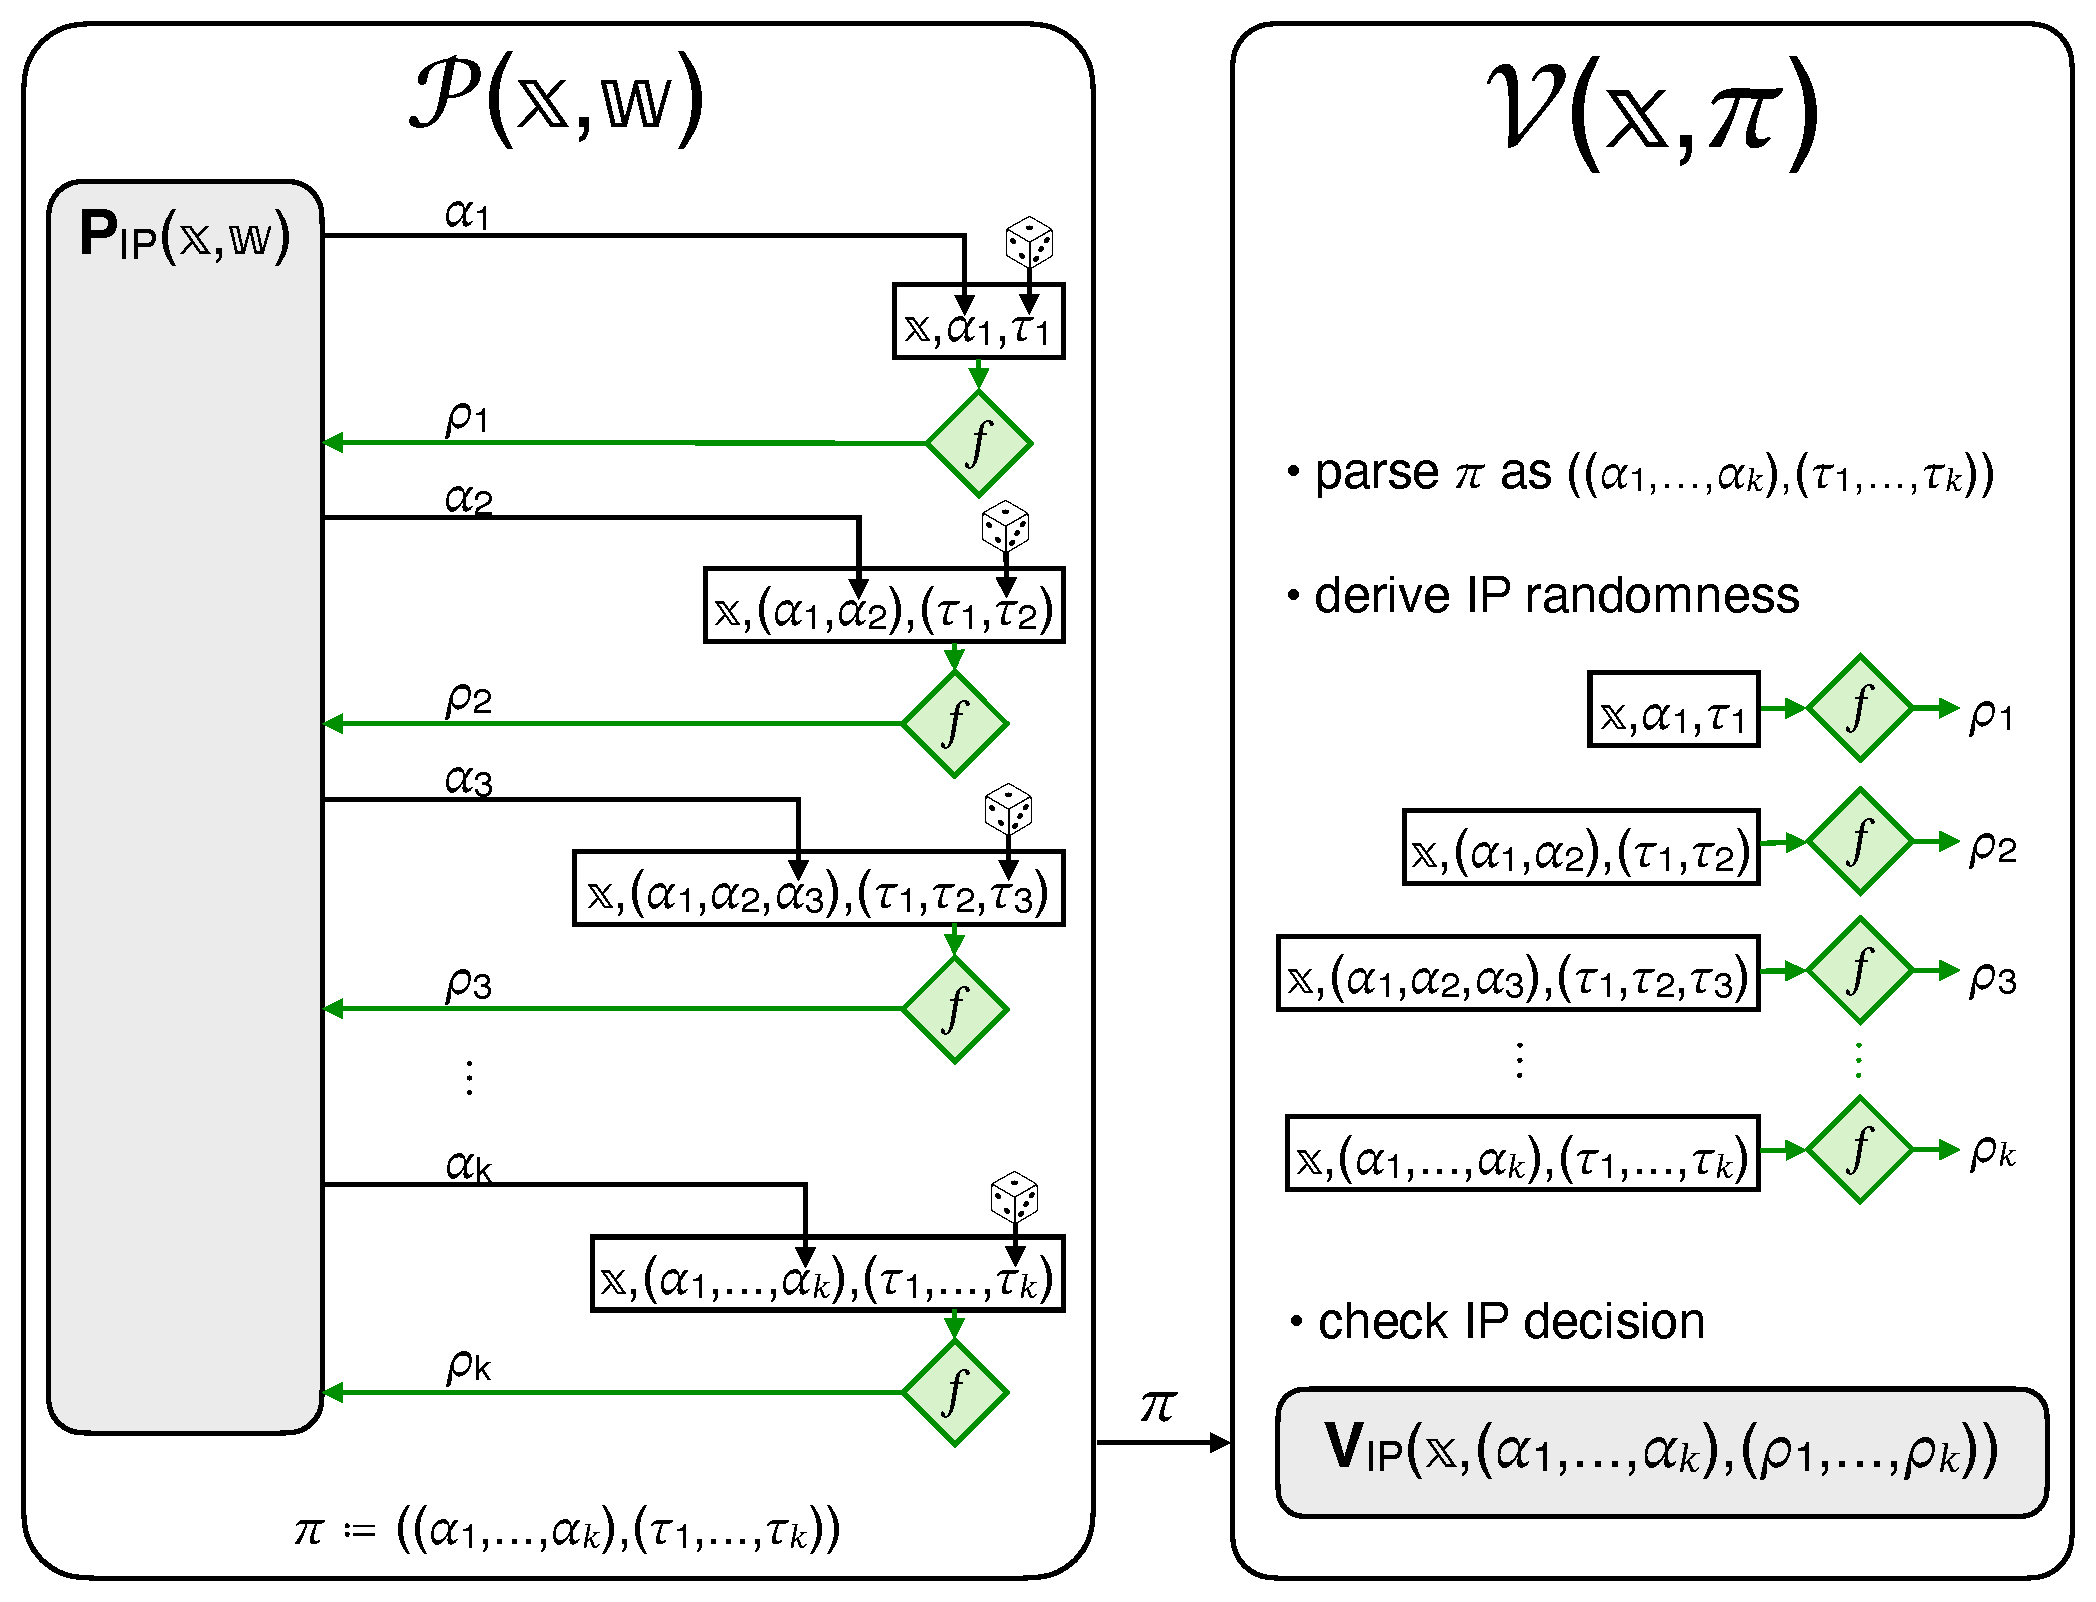
\includegraphics[width=0.85\textwidth]{\FigureFolder/slow-fs-ip-diagram}
\caption[Diagram of the FS transformation for public-coin IPs]{Diagram of the \FSonIPText ($\FSonIPSymbol$ in \Cref{construction:slow-fs-for-public-coin-ip}).}
\label{figure:slow-fs-for-ip-diagram}
\end{figure}

%%%%%%%%%%%%%%%%%%%%%%%%%%%%%%%%%%%%%%%%%%%%%%%%%%%%%%%%%%%%%%%%%%%%%%%%%%%%%%%
%%%%%%%%%%%%%%%%%%%%%%%%%%%%%%%%%%%%%%%%%%%%%%%%%%%%%%%%%%%%%%%%%%%%%%%%%%%%%%%
%%%%%%%%%%%%%%%%%%%%%%%%%%%%%%%%%%%%%%%%%%%%%%%%%%%%%%%%%%%%%%%%%%%%%%%%%%%%%%%
\section{Lower bound on the soundness error}
\label{section:slow-fs-attack-sr}

We show that every state-restoration attack on a public-coin IP translates into a corresponding attack on the resulting non-interactive argument (obtained via \Cref{construction:slow-fs-for-public-coin-ip}). Hence, a small state-restoration soundness error for the public-coin IP is \emph{necessary} for a small soundness error for the resulting non-interactive argument.\footnote{Having small soundness error does not imply having small state-restoration soundness error; see \Cref{remark:sr-tightness-of-upper-bound}.} Later in \Cref{section:slow-fs-reduction} we prove that a small state-restoration soundness error is also \emph{sufficient}.

The intuition is similar to the lower bound in \Cref{section:warmup-narg-from-sp-lower-bound} for the Fiat--Shamir transformation applied to SPs. Namely, while a malicious IP prover has a single chance to convince the IP verifier, a malicious argument prover for \Cref{construction:slow-fs-for-public-coin-ip} has \emph{multiple} chances to convince the IP verifier that underlies the argument verifier. Hence the soundness error of the non-interactive argument is greater than the soundness error of the IP.

In more detail, the malicious argument prover can \DoQuote{explore} different partial transcripts of interaction by querying the random oracle with different IP prover messages and salts, and eventually output an argument string $\ARGString = \FSARGString$ based on this information. For example, the malicious argument prover can first query the random oracle at $\FSFirstQuery$ to obtain the IP verifier challenge $\IPVerifierRandomMessage_{1}$, and subsequently explore two different extensions of this transcript: query the random oracle at $\big(\Instance,(\IPProverMessage_{1},\IPProverMessage_{2}),(\RandSaltString_{1},\RandSaltString_{2})\big)$ and $\big(\Instance,(\IPProverMessage_{1},\IPProverMessage_{2}'),(\RandSaltString_{1},\RandSaltString_{2})\big)$ for two different IP prover messages $\IPProverMessage_{2}$ and $\IPProverMessage_{2}'$ in order to obtain two different IP verifier challenges $\IPVerifierRandomMessage_{2}$ and $\IPVerifierRandomMessage_{2}'$. And so on. The malicious argument prover can also try its luck by outputting an argument string $\ARGString = \FSARGString$ for which it has not seen some of the corresponding randomness.

This type of exploration is exactly what is modeled by the IP state-restoration game in \Cref{definition:ip-state-restoration-game}. Indeed, we show that every IP state-restoration strategy can be directly translated into a strategy to convince the argument verifier in \Cref{construction:slow-fs-for-public-coin-ip} with (at least) the same convincing probability. In particular, the soundness error of the non-interactive argument is lower bounded by the underlying IP's state-restoration soundness error.

\begin{lemma}
\label{lemma:attack-against-narg-from-ip}
Let $\IPSymbol=\IPSystem$ be a public-coin IP for a relation $\Relation$ with state-restoration soundness error exactly $\IPSRSoundnessError$. For every security parameter $\SecurityParameter \in \Naturals$ and privacy parameter $\PrivacyParameter \in \Naturals$, $\NARGSymbol \DefineEqual \FSonIPTransformation{\IPSymbol}{\SecurityParameter}{\PrivacyParameter}$ in \Cref{construction:slow-fs-for-public-coin-ip} is a non-interactive argument for $\Relation$ with adaptive soundness error $\ARGSoundnessError$ (see \Cref{definition:narg-adaptive-soundness-with-cnf}) such that for every query bound $\ROQueryBound \in \Naturals$ and instance size bound $\InstanceSize \in \Naturals$,
\begin{equation*}
\ARGSoundnessError(\SecurityParameter,\ROQueryBound,\InstanceSize)
\geq
\IPSRSoundnessError(\SRSaltSize,\SRBudget,\InstanceSize)
\enspace.
\end{equation*}
\end{lemma}

\begin{construction}
\label{construction:attack-against-narg-from-ip}
Let $\IPMaliciousSRProver$ be a $\ROQueryBound$-move IP state-restoration prover for $\IPSymbol=\IPSystem$ that succeeds with probability $\IPSRSoundnessError(\SRSaltSize,\SRBudget,\InstanceSize)$. We construct a $\ROQueryBound$-query argument prover $\Malicious{\ARGProver}$ for $\NARGSymbol \DefineEqual \FSonIPTransformation{\IPSymbol}{\SecurityParameter}{\PrivacyParameter}$ that, given query access to random oracles $\IPTuple{\ROFunction} \in \RODistribution{\IPTuple{\IPRandomnessComplexity}}$ and black-box access to $\IPMaliciousSRProver$, works as follows.
\begin{enumerate}[noitemsep]
  \item Repeat the following $\ROQueryBound$ times (or until $\IPMaliciousSRProver$ decides to exit the loop):
  \begin{enumerate}[nolistsep]
    \item $\IPMaliciousSRProver$ outputs a move $\IPSRGameStateEntry{\RoundIndex}$;
    \item answer with $\ROFunction_{\RoundIndex}\IPSRGameStateEntry{\RoundIndex}$.
\end{enumerate}
  \item $\IPMaliciousSRProver$ outputs $\IPSRGameStateEntry{\IPRoundComplexity}$.
  \item For every $\RoundIndex \in [\IPRoundComplexity]$, set $\RandSaltString_{\RoundIndex} \DefineEqual \SRSaltString_{\RoundIndex}$.
  \item Set the argument string $\ARGString \DefineEqual \FSARGString$.
  \item Output $(\Instance,\ARGString)$.
\end{enumerate}
In other words, the argument prover $\Malicious{\ARGProver}$ emulates the IP state-restoration attack performed by $\IPMaliciousSRProver$, choosing randomness of the IP state-restoration game according to the random oracles $\IPTuple{\ROFunction}$.
\end{construction}

\begin{proof}
The lemma directly follows from the observation that $\IPMaliciousSRProver$ wins in the IP state-restoration game if and only if $\Malicious{\ARGProver}$ convinces the argument verifier, whenever the randomness choices are the same in both cases. (Randomness consists of a sample from $\RODistribution{\IPTuple{\IPRandomnessComplexity}}$.) We conclude that
\begin{align*}
& \Pr\left[
\begin{array}{l}
\SomeSize{\Instance} \leq \InstanceSize \\
\land\;\Instance \notin \GetLanguage{\Relation} \\
\land \; \ARGVerifier^{\ROFunction}(\Instance,\ARGString) = 1
\end{array}
\GivenExperiment
\StateExperiment{
\ROFunction=\IPTuple{\ROFunction} \gets \RODistribution{\IPTuple{\IPRandomnessComplexity}} \\
(\Instance,\ARGString) \gets \Malicious{\ARGProver}^{\ROFunction}(\BlackBox{\IPMaliciousSRProver})
}
\right]
\\ & =
\Pr\left[
\begin{array}{l}
\SomeSize{\Instance} \leq \InstanceSize \\
\land\;\Instance \notin \GetLanguage{\Relation} \\
\land\;\IPVerifier\big(\IPVerifierInput\big)=1
\end{array}
\GivenExperiment
\StateExperiment{
\SRRandomness=\IPTuple{\SRRandomness} \gets \RODistribution{\IPTuple{\IPRandomnessComplexity}} \\
\big(\IPVerifierInput\big) \gets \IPStateRestorationGame{\SRSaltSize}{\SRRandomness}{\IPMaliciousSRProver}
}
\right]
\enspace.
\end{align*}
\end{proof}

%%%%%%%%%%%%%%%%%%%%%%%%%%%%%%%%%%%%%%%%%%%%%%%%%%%%%%%%%%%%%%%%%%%%%%%%%%%%%%%
%%%%%%%%%%%%%%%%%%%%%%%%%%%%%%%%%%%%%%%%%%%%%%%%%%%%%%%%%%%%%%%%%%%%%%%%%%%%%%%
%%%%%%%%%%%%%%%%%%%%%%%%%%%%%%%%%%%%%%%%%%%%%%%%%%%%%%%%%%%%%%%%%%%%%%%%%%%%%%%
\section{Soundness}
\label{section:slow-fs-reduction}

We prove that \Cref{construction:slow-fs-for-public-coin-ip} is adaptively sound. The following theorem states that the adaptive soundness error of the non-interactive argument is upper bounded by the IP state-restoration soundness error of the underlying IP. In particular, a small state-restoration soundness error for the IP is \emph{sufficient} for a small adaptive soundness error for the resulting non-interactive argument.

\begin{ImportantTheorem}{}{slow-fs-for-public-coin-ip}
Let $\IPSymbol$ be a public-coin IP for a relation $\Relation$ with state-restoration soundness error $\IPSRSoundnessError$. For every security parameter $\SecurityParameter \in \Naturals$ and privacy parameter $\PrivacyParameter \in \Naturals$, $\NARGSymbol \DefineEqual \FSonIPTransformation{\IPSymbol}{\SecurityParameter}{\PrivacyParameter}$ in \Cref{construction:slow-fs-for-public-coin-ip} is a non-interactive argument for $\Relation$ with adaptive soundness error $\ARGSoundnessError$ (see \Cref{definition:narg-adaptive-soundness-with-cnf}) such that
\begin{equation*}
\ARGSoundnessError(\SecurityParameter,\ROQueryBound,\InstanceSize)
\leq
\IPSRSoundnessError(\PrivacyParameter,\ROQueryBound,\InstanceSize)
\enspace.
\end{equation*}
\end{ImportantTheorem}

\begin{proof}
Fix a query bound $\ROQueryBound \in \Naturals$, $\ROQueryBound$-query argument prover $\Malicious{\ARGProver}$, and instance size bound $\InstanceSize \in \Naturals$. In \Cref{construction:slow-fs-sr-prover} we describe an IP state-restoration prover $\IPMaliciousSRProver$ that, using $\Malicious{\ARGProver}$ as a black box, wins the IP state-restoration soundness game with (at least) the same probability as $\Malicious{\ARGProver}$ convinces the argument verifier $\ARGVerifier$. Specifically, \Cref{lemma:slow-fs-sr-prover} upper bounds the winning probability of the argument prover $\Malicious{\ARGProver}$ by the winning probability of the IP state-restoration prover $\IPMaliciousSRProver$.
\end{proof}

\begin{construction}
\label{construction:slow-fs-sr-prover}
The IP state-restoration prover $\IPMaliciousSRProver$ is parametrized by the security parameter $\SecurityParameter$ and instance size bound $\InstanceSize$ and receives an argument prover $\BlackBox{\Malicious{\ARGProver}}$ as a black box.
\begin{enumerate}[noitemsep]
  \item For every $\RoundIndex \in [\IPRoundComplexity]$, lazily sample an oracle $\LazySub{\ROFunctionAlt}{\RoundIndex} \gets \RODistribution{\IPRandomnessComplexity_{\RoundIndex}}$ (to answer malformed queries).
  \item Simulate $\Malicious{\ARGProver}$ while answering a query $\ROQuery$ to $\ROFunction_{\RoundIndex}$ as follows:
  \begin{enumerate}[noitemsep]
    \item If $\ROQuery$ can be parsed as a tuple $\SlowFSLaterQuery{\RoundIndex}$:
    \begin{enumerate}[nolistsep]
      \item Output the move $\SlowFSLaterQuery{\RoundIndex}$ to the IP state-restoration game.
      \item Receive the response $\IPVerifierRandomMessage_{\RoundIndex}$ from the IP state-restoration game.
    \end{enumerate}
    \item Otherwise set $\IPVerifierRandomMessage_{\RoundIndex} \DefineEqual \LazySub{\ROFunctionAlt}{\RoundIndex}(\ROQuery)$.
    \item Return $\IPVerifierRandomMessage_{\RoundIndex}$ as the answer to the query.
  \end{enumerate}
  \item The simulation of $\Malicious{\ARGProver}$ ends with an output $(\Instance,\ARGString)$, where $\ARGString = \FSARGString$.
  \item For every $\RoundIndex \in [\IPRoundComplexity]$, set the salt string $\SRSaltString_{\RoundIndex} \DefineEqual \RandSaltString_{\RoundIndex}$.
  \item The final output is $\IPSRGameStateEntry{\IPRoundComplexity}$.
\end{enumerate}
The IP state-restoration prover $\IPMaliciousSRProver$ makes at most $\ROQueryBound$ moves in the IP state-restoration game, since $\IPMaliciousSRProver$ makes at most one move for each query of $\Malicious{\ARGProver}$ (which makes at most $\ROQueryBound$ queries). Moreover the running time of $\IPMaliciousSRProver$ is at most the running time of $\Malicious{\ARGProver}$ plus $O(\IPMaxRandomnessComplexity \cdot \ROQueryBound)$.
\end{construction}

\begin{construction}
\label{construction:slow-to-sr-trace}
The function $\FSToSR$ receives as input a query-answer trace $\ROTrace$ and outputs a move-response trace $\SRTrace$ computed as follows.
\begin{itemize}[noitemsep]
  \item[] $\FSToSR(\ROTrace)$:
  \begin{enumerate}[nolistsep]
    \item Initialize an empty list of move-response pairs $\SRTrace$.
    \item For each query-answer $(\ROQuery,\ROAnswer)$ in $\ROTrace$ (taken in order): if $\ROQuery$ is a query to $\ROFunction_{\RoundIndex}$ and can be parsed as a tuple $\SlowFSLaterQuery{\RoundIndex}$, append $(\ROQuery,\ROAnswer)$ to $\SRTrace$.
    \item Output $\SRTrace$.
  \end{enumerate}
\end{itemize}
If $\Malicious{\ARGProver}$ has query-answer trace $\ROTrace$ then $\IPMaliciousSRProver(\BlackBox{\Malicious{\ARGProver}})$ has a move-response trace $\SRTrace$ (in the IP state-restoration game) that is output by the procedure $\FSToSR$. The running time of $\FSToSR$ is $O(\IPMaxRandomnessComplexity \cdot \ROQueryBound)$, as processing each of at most $\ROQueryBound$ query-answer pairs takes time $O(\IPMaxRandomnessComplexity)$.
\end{construction}

\begin{lemma}
\label{lemma:slow-fs-sr-prover}
$\IPMaliciousSRProver$ in \Cref{construction:slow-fs-sr-prover} is such that
\begin{align*}
& \Pr\left[
\begin{array}{l}
\SomeSize{\Instance} \leq \InstanceSize \\
\land\;\Instance \notin \GetLanguage{\Relation} \\
\land\;\ARGVerifier^{\ROFunction}(\Instance,\ARGString) = 1
\end{array}
\GivenExperiment
\StateExperiment{
\ROFunction=\IPTuple{\ROFunction} \gets \RODistribution{\IPTuple{\IPRandomnessComplexity}} \\
(\Instance,\ARGString) \gets \Malicious{\ARGProver}^{\ROFunction}
}
\right]
\\ & \leq
\Pr\left[
\begin{array}{l}
\SomeSize{\Instance} \leq \InstanceSize \\
\land\;\Instance \notin \GetLanguage{\Relation} \\
\land\;\IPVerifier\big(\IPVerifierInput\big)=1
\end{array}
\GivenExperiment
\StateExperiment{
\SRRandomness=\IPTuple{\SRRandomness} \gets \RODistribution{\IPTuple{\IPRandomnessComplexity}} \\
\LongExecution{\IPSROutput}{\IPStateRestorationGame{\SRSaltSize}{\SRRandomness}{\IPMaliciousSRProver(\BlackBox{\Malicious{\ARGProver}})}} \\
}
\right]
\enspace.
\end{align*}
Moreover, if the running time of $\Malicious{\ARGProver}$ is $\ARGTimeP$ then the running time of $\IPMaliciousSRProver$ is $\ARGTimeP + O(\IPMaxRandomnessComplexity \cdot \ROQueryBound)$.
\end{lemma}

\begin{proof}
It suffices to prove the inequality for an arbitrary choice of randomness for $\Malicious{\ARGProver}$ (in case $\Malicious{\ARGProver}$ is not deterministic), so fix such a choice of randomness. The proof of the lemma follows immediately from the following equivalence of distributions:
\begin{align}
\label{eq:slow-fs-sr-prover}
&\left\{
(\SRTrace,\IPTuple{\IPVerifierRandomMessage},\Instance,\ARGString,\DecisionBit)
\GivenExperiment
\StateExperiment{
\ROFunction=\IPTuple{\ROFunction} \gets \RODistribution{\IPTuple{\IPRandomnessComplexity}} \\
\ROOutputAndTrace{\ROFunction}{\Malicious{\ARGProver}}{\ROTrace}{(\Instance,\ARGString)} \\
\DecisionBit \xleftarrow{\ROTraceVerifier} \ARGVerifier^{\ROFunction}(\Instance,\ARGString) \\
\SRTrace \DefineEqual \FSToSR(\ROTrace) \\
\text{parse} \; \ROTraceVerifier \; \text{as} \;  (\ROQuery_{\RoundIndex},\IPVerifierRandomMessage_{\RoundIndex})_{\RoundIndex \in [\IPRoundComplexity]} \\
}
\right\}
\\ \equiv &
\left\{
(\SRTrace,\IPTuple{\IPVerifierRandomMessage},\Instance,\ARGString,\DecisionBit)
\GivenExperiment
\StateExperiment{
\SRRandomness=\IPTuple{\SRRandomness} \gets \RODistribution{\IPTuple{\IPRandomnessComplexity}} \\
\ShortExecutionOver{\IPSROutput}{\IPStateRestorationGame{\SRSaltSize}{\SRRandomness}{\IPMaliciousSRProver(\BlackBox{\Malicious{\ARGProver}})}}{\SRTrace} \\
\IPTuple{\RandSaltString} \DefineEqual \IPTuple{\SRSaltString} \\
\ARGString \DefineEqual \FSARGString \\
\DecisionBit \gets \IPVerifier\big(\IPVerifierInput\big)
}
\right\}
\enspace. \nonumber
\end{align}
We argue that $(\SRTrace,\IPTuple{\IPVerifierRandomMessage},\Instance,\ARGString,\DecisionBit)$ is identically distributed in both experiments.

The cheating argument prover $\Malicious{\ARGProver}$ receives the same distribution of query answers in both sides: in the left-side experiment $\Malicious{\ARGProver}$ receives answers from the random oracles $\IPTuple{\ROFunction}$; and in the right-side experiment $\Malicious{\ARGProver}$ receives answers either from the IP state-restoration prover $\IPMaliciousSRProver$ (which in turn receives answers from the IP state restoration game with randomness $\IPTuple{\SRRandomness}$) or from the auxiliary oracles $(\LazySub{\ROFunctionAlt}{\RoundIndex})_{\RoundIndex \in [\IPRoundComplexity]}$ (which are lazily sampled). In both cases, unique queries get independent random answers, and duplicate queries are answered consistently.

Hence the output $(\Instance,\ARGString)$ of $\Malicious{\ARGProver}$ in both experiments is equally distributed. (In the right-side experiment $\ARGString$ is disassembled within the IP state-restoration game and reassembled outside of it.)

Next we discuss the decision bit $\DecisionBit$ and the randomness $\IPTuple{\IPVerifierRandomMessage}$ in both experiments.
\begin{itemize}
  \item \emph{Left-side experiment.}
  The bit $\DecisionBit$ is $\ARGVerifier^{\ROFunction}(\Instance,\ARGString)$. By construction of the argument verifier $\ARGVerifier$ and recalling that $\ARGString = \FSARGString$, the bit $\DecisionBit$ is $\IPVerifier\big(\IPVerifierInput\big)$ where $\IPVerifierRandomMessage_{\RoundIndex} \DefineEqual \ROFunction_{\RoundIndex}\SlowFSLaterQuery{\RoundIndex}$ for every $\RoundIndex \in [\IPRoundComplexity]$.
  \item \emph{Right-side experiment.}
  By definition of the IP state-restoration game, the bit $\DecisionBit$ is equal to $\IPVerifier\big(\IPVerifierInput\big)$ where $\Instance$ is the instance output by $\Malicious{\ARGProver}$, $\ARGString=\FSARGString$ is the argument string output by $\Malicious{\ARGProver}$, and $\IPVerifierRandomMessage_{\RoundIndex} \DefineEqual \SRRandomness_{\RoundIndex}\SlowFSLaterQuery{\RoundIndex}$ for every $\RoundIndex \in [\IPRoundComplexity]$.
\end{itemize}
Recalling that $\ROFunction=\IPTuple{\ROFunction}$ and $\SRRandomness=\IPTuple{\SRRandomness}$ have the same distribution in both experiments, we deduce that the decision bit $\DecisionBit$, and the random values $\IPTuple{\IPVerifierRandomMessage}$ have the same distribution in both experiments.

Finally, $\FSToSR(\ROTrace)$ removes queries in $\ROTrace$ that are not well-formed and $\IPMaliciousSRProver$ forwards (and only forwards) well-formed queries of $\Malicious{\ARGProver}$ to the IP state-restoration game, so $\FSToSR(\ROTrace)$ in the left-side experiment and $\SRTrace$ in the right-side experiment have the same distribution.
\end{proof}

\begin{remark}[the case of SPs]
\label{remark:fs-ip-implies-sigma}
An SP is a special case of a public-coin IP where the verifier sends a single random challenge and, in particular, the notions of state restoration for SPs in \Cref{section:sp-sr-definition} are special cases of the notions of state restoration for IPs in \Cref{section:fs-sr-definition}. Moreover, \Cref{construction:fs-for-sp} (NARG from an SP) is a special case of \Cref{construction:slow-fs-for-public-coin-ip} (NARG from an IP) and, correspondingly, \Cref{lemma:fs-for-sigma-protocol-adaptive-soundness} ($\ARGSoundnessError(\SecurityParameter,\ROQueryBound,\InstanceSize) \leq \SPSRSoundnessError(\PrivacyParameter,\ROQueryBound,\InstanceSize)$) is a special case of \Cref{theorem:slow-fs-for-public-coin-ip} ($\ARGSoundnessError(\SecurityParameter,\ROQueryBound,\InstanceSize) \leq \IPSRSoundnessError(\PrivacyParameter,\ROQueryBound,\InstanceSize)$). Finally, \Cref{lemma:sp-srs-to-soundness} tells us that the SP state-restoration soundness error for an SP is at most $\SRBudget+1$ times the soundness error of the SP: $\SPSRSoundnessError(\PrivacyParameter,\SRBudget,\InstanceSize) \leq (\SRBudget+1) \cdot \SPSoundnessError(\InstanceSize)$. Hence, if we apply \Cref{theorem:slow-fs-for-public-coin-ip} to an SP then we get that the adaptive soundness error of the resulting non-interactive argument is upper bounded as follows:
\begin{equation*}
\ARGSoundnessError(\SecurityParameter,\ROQueryBound,\InstanceSize)
\leq
\IPSRSoundnessError(\PrivacyParameter,\ROQueryBound,\InstanceSize)
=
\SPSRSoundnessError(\PrivacyParameter,\ROQueryBound,\InstanceSize)
\leq
(\ROQueryBound+1) \cdot \SPSoundnessError(\InstanceSize)
\enspace.
\end{equation*}
Thus we recover the same upper bound as in \Cref{theorem:narg-from-sp-adaptive-soundness} for \Cref{construction:fs-for-sp}.

A similar discussion holds for knowledge soundness rather than soundness.
\end{remark}

\begin{remark}[on adaptive security]
\label{remark:adaptivity-in-slow-fs}
In \Cref{construction:slow-fs-for-public-coin-ip} every query to the random oracle (by the argument prover and by the argument verifier) includes the instance $\Instance$. This is consistent with the generic transformation to achieve adaptive security in \Cref{section:non-adaptive-security}. However, unlike \Cref{section:non-adaptive-security}, the upper bound on the adaptive soundness error in \Cref{theorem:slow-fs-for-public-coin-ip} does not have a multiplicative factor of $\ROQueryBound$ (when compared to the non-adaptive soundness error). This is because we give a direct proof of adaptive soundness for this construction.
\end{remark}



%%%%%%%%%%%%%%%%%%%%%%%%%%%%%%%%%%%%%%%%%%%%%%%%%%%%%%%%%%%%%%%%%%%%%%%%%%%%%%%
%%%%%%%%%%%%%%%%%%%%%%%%%%%%%%%%%%%%%%%%%%%%%%%%%%%%%%%%%%%%%%%%%%%%%%%%%%%%%%%
%%%%%%%%%%%%%%%%%%%%%%%%%%%%%%%%%%%%%%%%%%%%%%%%%%%%%%%%%%%%%%%%%%%%%%%%%%%%%%%
\section{Knowledge soundness}
\label{section:slow-fs-knowledge-soundness}

We prove that \Cref{construction:slow-fs-for-public-coin-ip} satisfies (adaptive) knowledge soundness. The following theorem states that the adaptive knowledge soundness error of the non-interactive argument is upper bounded by the IP state-restoration knowledge soundness error of the underlying IP.

\begin{ImportantTheorem}{}{slow-fs-knowledge-soundness}
Let $\IPSymbol$ be a public-coin IP for a relation $\Relation$ with rewinding state-restoration knowledge soundness error $\IPSRKnowledgeError$ with extraction time $\IPKnowledgeTime$ (see \Cref{definition:ip-state-restoration-knowledge}). For every security parameter $\SecurityParameter \in \Naturals$ and privacy parameter $\PrivacyParameter \in \Naturals$, $\NARGSymbol \DefineEqual \FSonIPTransformation{\IPSymbol}{\SecurityParameter}{\PrivacyParameter}$ in \Cref{construction:slow-fs-for-public-coin-ip} is a non-interactive argument for $\Relation$ with rewinding knowledge soundness error $\ARGKnowledgeError$ with extraction time $\ARGKnowledgeTime$ (see \Cref{definition:adaptive-rewinding-knowledge-soundness-with-cnf}) such that
\begin{itemize}[nolistsep]
  \item $\ARGKnowledgeError(\SecurityParameter,\ROQueryBound,\InstanceSize,\ProverFailureProbability{\Malicious{\ARGProver}}(\SecurityParameter,\InstanceSize)) \leq \IPSRKnowledgeError\left(\PrivacyParameter,\ROQueryBound,\InstanceSize,\ProverFailureProbability{\Malicious{\ARGProver}}(\SecurityParameter,\InstanceSize)\right)$, and
  \item $\ARGKnowledgeTime(\SecurityParameter,\ROQueryBound,\InstanceSize, \ProverFailureProbability{\Malicious{\ARGProver}}(\SecurityParameter,\InstanceSize),\ProverRunningTime{\Malicious{\ARGProver}}(\SecurityParameter,\InstanceSize)) \leq \IPSRKnowledgeTime\left(\PrivacyParameter,\ROQueryBound,\InstanceSize,\ProverFailureProbability{\Malicious{\ARGProver}}(\SecurityParameter,\InstanceSize),\ProverRunningTime{\Malicious{\ARGProver}}(\SecurityParameter,\InstanceSize)+O(\IPMaxRandomnessComplexity \cdot \ROQueryBound)\right) + O(\IPMaxRandomnessComplexity \cdot \ROQueryBound)$.
\end{itemize}
Moreover, if the IP state-restoration extractor is straightline (see \Cref{definition:ip-state-restoration-knowledge-straightline}) then the NARG extractor is also straightline (see \Cref{definition:adaptive-straightline-knowledge-soundness-with-cnf}). In this case:
\begin{itemize}[nolistsep]
  \item the (straightline) knowledge soundness error is $\ARGKnowledgeError(\SecurityParameter,\ROQueryBound,\InstanceSize) \leq \IPSRKnowledgeError(\PrivacyParameter,\ROQueryBound,\InstanceSize)$; and
  \item the (straightline) extraction time is $\ARGKnowledgeTime(\SecurityParameter,\ROQueryBound,\InstanceSize) \leq \IPSRKnowledgeTime(\PrivacyParameter,\ROQueryBound,\InstanceSize) + O(\IPMaxRandomnessComplexity \cdot \ROQueryBound)$.
\end{itemize}
\end{ImportantTheorem}

\begin{construction}
\label{construction:slow-fs-extractor}
Let $\IPSRExtractor$ be the IP state-restoration extractor for $\IPSymbol$. Let $\FSToSR$ be the trace translation procedure in \Cref{construction:slow-to-sr-trace}. The extractor $\ARGExtractor$ for $\NARGSymbol$ receives as input an instance $\Instance$, argument string $\ARGString$, query-answer trace $\ROTrace$ of the argument prover, query-answer trace $\ROTraceVerifier$ of the argument verifier, and black-box access to the argument prover $\Malicious{\ARGProver}$, and works as follows.
\begin{itemize}[noitemsep]
\item[] $\ARGExtractor(\Instance,\ARGString,\ROTrace,\ROTraceVerifier, \BlackBox{\Malicious{\ARGProver}})$:
\begin{enumerate}[nolistsep]
  \item Parse $\ARGString$ as a tuple $\FSARGString$.
  \item Compute the move-response trace from the query-answer trace: $\SRTrace \DefineEqual \FSToSR(\ROTrace)$.
  \item Parse the trace $\ROTraceVerifier$ as $\IPRoundComplexity$ query-answer pairs $\left(\left(\SlowFSLaterQuery{\RoundIndex},\IPVerifierRandomMessage_{\RoundIndex}\right)\right)_{\RoundIndex \in [\IPRoundComplexity]}$.
  \item Use $\Malicious{\ARGProver}$ to construct the IP state-restoration prover $\IPMaliciousSRProver \DefineEqual \IPMaliciousSRProver(\BlackBox{\Malicious{\ARGProver}})$ in \Cref{construction:slow-fs-sr-prover}.
  \item Compute the witness: $\Witness \gets \IPSRExtractor(\Instance,\IPTuple{\IPProverMessage},\IPTuple{\RandSaltString},\IPTuple{\IPVerifierRandomMessage},\SRTrace,\BlackBox{\IPMaliciousSRProver})$.
  \item Output $\Witness$.
\end{enumerate}
\end{itemize}
\end{construction}

\begin{proof}
Fix a $\ROQueryBound$-query malicious argument prover $\Malicious{\ARGProver}$. We upper bound the rewinding knowledge soundness error as follows:
\begin{align*}
&\Pr\left[
\begin{array}{l}
  \SomeSize{\Instance} \leq \InstanceSize \\
  \land\;(\Instance,\Witness) \notin \Relation \\
  \land\;\DecisionBit = 1
\end{array}
\GivenExperiment
\StateExperiment{
  \ROFunction \gets \RODistribution{\IPTuple{\IPRandomnessComplexity}} \\
  \ROOutputAndTrace{\ROFunction}{\Malicious{\ARGProver}}{\ROTrace}{(\Instance,\ARGString)} \\
  \DecisionBit \xleftarrow{\ROTraceVerifier} \ARGVerifier^{\ROFunction}(\Instance,\ARGString) \\
  \Witness \gets \ARGExtractor(\Instance,\ARGString,\ROTrace, \ROTraceVerifier, \BlackBox{\Malicious{\ARGProver}})
}
\right]
\\ & =
\Pr\left[
\begin{array}{l}
  \SomeSize{\Instance} \leq \InstanceSize \\
  \land\;(\Instance,\Witness) \notin \Relation \\
  \land\;\DecisionBit = 1
\end{array}
\GivenExperiment
\StateExperiment{
  \ROFunction \gets \RODistribution{\IPTuple{\IPRandomnessComplexity}} \\
  \ROOutputAndTrace{\ROFunction}{\Malicious{\ARGProver}}{\ROTrace}{(\Instance,\FSARGString)} \\
  \DecisionBit \xleftarrow{\ROTraceVerifier} \ARGVerifier^{\ROFunction}(\Instance,\FSARGString) \\
  \SRTrace \DefineEqual \FSToSR(\ROTrace) \\
  \ROTraceVerifier = \left(\left(\SlowFSLaterQuery{\RoundIndex},\IPVerifierRandomMessage_{\RoundIndex}\right)\right)_{\RoundIndex \in [\IPRoundComplexity]} \\
  \Witness \gets \IPSRExtractor(\Instance,\IPTuple{\IPProverMessage},\IPTuple{\RandSaltString},\IPTuple{\IPVerifierRandomMessage},\SRTrace,\BlackBox{\IPMaliciousSRProver(\BlackBox{\Malicious{\ARGProver}})})
}
\right]
\\ & \; \EquationComment{by definition of $\ARGExtractor$}
\\ & \leq
\Pr\left[
\begin{array}{l}
  \SomeSize{\Instance} \leq \InstanceSize \\
  \land\;(\Instance,\Witness) \notin \Relation \\
   \land\;\IPVerifier\big(\IPVerifierInput\big)
\end{array}
\GivenExperiment
\StateExperiment{
  \SRRandomness=\IPTuple{\SRRandomness} \gets \RODistribution{\IPTuple{\IPRandomnessComplexity}} \\
  \LongExecutionOver{\IPSROutput}{\IPStateRestorationGame{\SRSaltSize}{\SRRandomness}{\IPMaliciousSRProver}}{\SRTrace} \\
  \Witness \gets \IPSRExtractor(\Instance,\IPTuple{\IPProverMessage},\SRSaltStrings{\IPRoundComplexity},\IPTuple{\IPVerifierRandomMessage},\SRTrace,\BlackBox{\IPMaliciousSRProver(\BlackBox{\Malicious{\ARGProver}})})
}
\right]
\\ & \; \EquationComment{by \Cref{eq:slow-fs-sr-prover}}
\\ & \leq
\IPSRKnowledgeError(\PrivacyParameter,\ROQueryBound,\InstanceSize,\ProverFailureProbability{\IPMaliciousSRProver})
\EquationComment{by definition of $\IPSRKnowledgeError$}
\\ & \leq
\IPSRKnowledgeError(\PrivacyParameter,\ROQueryBound,\InstanceSize,\ProverFailureProbability{\Malicious{\ARGProver}})
\EquationComment{since $\ProverFailureProbability{\IPMaliciousSRProver} \leq \ProverFailureProbability{\Malicious{\ARGProver}}$ by \Cref{eq:slow-fs-sr-prover}}
\enspace.
\end{align*}
The running time of $\ARGExtractor$ on $\Malicious{\ARGProver}$ equals the running time of $\FSToSR$ plus the running time of $\IPSRExtractor$ on $\IPMaliciousSRProver(\BlackBox{\Malicious{\ARGProver}})$:
\begin{equation*}
\ARGKnowledgeTime(\SecurityParameter,\ROQueryBound,\InstanceSize,\ProverFailureProbability{\Malicious{\ARGProver}},\ProverRunningTime{\Malicious{\ARGProver}})
\leq
O(\IPMaxRandomnessComplexity \cdot \ROQueryBound)
+
\IPSRKnowledgeTime(\PrivacyParameter,\ROQueryBound,\InstanceSize,\ProverFailureProbability{\IPMaliciousSRProver},\ProverRunningTime{\IPMaliciousSRProver})
\enspace.
\end{equation*}
Since $\ProverFailureProbability{\IPMaliciousSRProver} \leq \ProverFailureProbability{\Malicious{\ARGProver}}$ (by \Cref{eq:slow-fs-sr-prover}), $\ProverRunningTime{\IPMaliciousSRProver} \leq \ProverRunningTime{\Malicious{\ARGProver}}+O(\IPMaxRandomnessComplexity \cdot \ROQueryBound)$ (as discussed in \Cref{construction:slow-fs-sr-prover}), and $\IPSRKnowledgeTime$ is non-decreasing in the failure probability and running time of the prover, we deduce that
\begin{equation*}
\IPSRKnowledgeTime(\PrivacyParameter,\ROQueryBound,\InstanceSize,\ProverFailureProbability{\IPMaliciousSRProver},\ProverRunningTime{\IPMaliciousSRProver})
\leq
\IPSRKnowledgeTime(\PrivacyParameter,\ROQueryBound,\InstanceSize,\ProverFailureProbability{\Malicious{\ARGProver}},\ProverRunningTime{\Malicious{\ARGProver}}+O(\IPMaxRandomnessComplexity \cdot \ROQueryBound))
\enspace,
\end{equation*}
which yields the extraction time bound in the lemma statement.

\parhead{The straightline case}
The above analysis directly specializes to the straightline case. Suppose that $\IPSRExtractor$ is a straightline extractor (\Cref{definition:ip-state-restoration-knowledge-straightline}): it is a deterministic algorithm that does not need access to the IP state-restoration prover $\IPMaliciousSRProver$. Then $\ARGExtractor$ in \Cref{construction:slow-fs-extractor} is a straightline extractor (\Cref{definition:adaptive-straightline-knowledge-soundness-with-cnf}): there is no need to construct $\IPMaliciousSRProver$ from $\Malicious{\ARGProver}$, and in particular no need to receive $\Malicious{\ARGProver}$. In this case $\IPSRKnowledgeError$ does not depend on the failure probability of $\IPMaliciousSRProver(\BlackBox{\Malicious{\ARGProver}})$, so the (straightline) knowledge soundness error bound simplifies to $\ARGKnowledgeError(\SecurityParameter,\ROQueryBound,\InstanceSize) \leq \IPSRKnowledgeError(\PrivacyParameter,\ROQueryBound,\InstanceSize)$. Moreover, the running time $\IPSRKnowledgeTime$ of $\IPSRExtractor$ does not depend on the failure probability or running time of $\IPMaliciousSRProver(\BlackBox{\Malicious{\ARGProver}})$, so the extraction time bound simplifies to $\ARGKnowledgeTime(\SecurityParameter,\ROQueryBound,\InstanceSize) \leq \IPSRKnowledgeTime(\PrivacyParameter,\ROQueryBound,\InstanceSize) + O(\IPMaxRandomnessComplexity \cdot \ROQueryBound)$ (the running time of $\IPSRExtractor$ plus the running time of $\FSToSR$).
\end{proof}

%%%%%%%%%%%%%%%%%%%%%%%%%%%%%%%%%%%%%%%%%%%%%%%%%%%%%%%%%%%%%%%%%%%%%%%%%%%%%%%
%%%%%%%%%%%%%%%%%%%%%%%%%%%%%%%%%%%%%%%%%%%%%%%%%%%%%%%%%%%%%%%%%%%%%%%%%%%%%%%
%%%%%%%%%%%%%%%%%%%%%%%%%%%%%%%%%%%%%%%%%%%%%%%%%%%%%%%%%%%%%%%%%%%%%%%%%%%%%%%
%%%%%%%%%%%%%%%%%%%%%%%%%%%%%%%%%%%%%%%%%%%%%%%%%%%%%%%%%%%%%%%%%%%%%%%%%%%%%%%
\chapter{Optimization: a faster variant}
\label{chapter:fast-fs-for-ip}

In \Cref{chapter:slow-fs-for-ip} we discussed how to transform any public-coin interactive proof (IP) into a corresponding non-interactive argument, via \Cref{construction:slow-fs-for-public-coin-ip}. Here we study a faster variant of that construction: in \Cref{section:fast-fs-for-ip} we highlight an inefficiency and describe how to resolve it via a modified construction; and in \Cref{section:fast-fs-reduction} we analyze the soundness of the modified construction. Later in \Cref{chapter:fs-additional} we study additional security definitions for this modified construction.

%%%%%%%%%%%%%%%%%%%%%%%%%%%%%%%%%%%%%%%%%%%%%%%%%%%%%%%%%%%%%%%%%%%%%%%%%%%%%%%
%%%%%%%%%%%%%%%%%%%%%%%%%%%%%%%%%%%%%%%%%%%%%%%%%%%%%%%%%%%%%%%%%%%%%%%%%%%%%%%
%%%%%%%%%%%%%%%%%%%%%%%%%%%%%%%%%%%%%%%%%%%%%%%%%%%%%%%%%%%%%%%%%%%%%%%%%%%%%%%
\section{Construction}
\label{section:fast-fs-for-ip}

We describe an inefficiency of \Cref{construction:slow-fs-for-public-coin-ip} and then describe a modified construction that addresses this inefficiency.

\parhead{Problem 1: quadratic blowup in hashing}
In \Cref{construction:slow-fs-for-public-coin-ip}, for every $\RoundIndex>1$, the $\RoundIndex$-th query to the random oracle $\ROQuery_{\RoundIndex} \DefineEqual \SlowFSLaterQuery{\RoundIndex}$ contains within it the $(\RoundIndex-1)$-th query $\ROQuery_{\RoundIndex-1} \DefineEqual \SlowFSLaterQuery{\RoundIndex-1}$ to the random oracle. Therefore:
\begin{inparaenum}[(i)]
  \item the instance $\Instance$ appears in $\IPRoundComplexity$ queries; and
  \item each IP prover message $\IPProverMessage_{\RoundIndex}$ and each salt $\RandSaltString_{\RoundIndex}$ appears in $\IPRoundComplexity-\RoundIndex+1$ queries.
\end{inparaenum}
This redundant structure creates a \DoQuote{quadratic cost} in the total size of the queries (that is visually evident in \Cref{figure:slow-fs-for-ip-diagram}):
\begin{equation*}
\sum_{\RoundIndex \in [\IPRoundComplexity]}
\BitSize{\ROQuery_{\RoundIndex}}
=
\IPRoundComplexity \cdot \BitSize{\Instance}
+
\sum_{\RoundIndex \in [\IPRoundComplexity]}
(\IPRoundComplexity-\RoundIndex+1) \cdot (\BitSize{\IPProverMessage_{\RoundIndex}}+\RandSaltSize)
=
\Omega(\IPRoundComplexity^2)
\enspace.
\end{equation*}
While this structure in the queries is precisely what ensures a chronological order, the structure also leads to the quadratic cost.

\parhead{Solution 1: hash chain}
The aforementioned quadratic cost can be reduced to linear by modifying the construction to use a \DoQuote{hash chain}. The intuition is that each query includes a hash of the previous query, rather than the previous query itself. This creates a \DoQuote{hash chain} structure that enforces the desired chronological order of the $\IPRoundComplexity$ queries. In more detail, the first query remains $\ROQuery_{1} \DefineEqual \FSFirstQuery$ as before, and its answer serves as the first IP verifier challenge $\IPVerifierRandomMessage_{1}$. The answer $\IPVerifierRandomMessage_{1}$ additionally serves as the hash of the prior query, which we include in the second query: we define the second query to be $\ROQuery_{2} \DefineEqual (\IPVerifierRandomMessage_{1},\IPProverMessage_{2},\RandSaltString_{2})$. The answer to this second query is $\IPVerifierRandomMessage_{2}$, which serves as the second IP verifier challenge as well as the hash of the second query. In general, for every $\RoundIndex \in \{2,\dots,\IPRoundComplexity\}$, the $\RoundIndex$-th query is $\FastFSLaterQuery{\RoundIndex}$. This hashing pattern is known as the \emph{Merkle--Damg\r{a}rd construction}, and it is commonly used to hash messages whose size is bigger than a hash function's input size. Here we use the fact that the hashing is incremental, which (intuitively) ensures that the IP verifier challenges are appropriately interleaved between IP prover messages.

\parhead{Problem 2: attacks to the hash chain}
The hash chain must be secure against attacks, in particular ensuring that, for every $\RoundIndex \in \{2,\dots,\IPRoundComplexity\}$, if an adversary makes a query $\FastFSLaterQuery{\RoundIndex}$ to the oracle $\ROFunction_{\RoundIndex}$ then the adversary is committed to (at most) one tuple $\SlowFSLaterQuery{\RoundIndex-1}$ that includes a choice of instance, prior messages, and prior salts. If the adversary were to find a collision or invert an element in the hash chain, then the adversary may \emph{not} be committed to (at most) one such tuple. The success probability of such attacks for round $\RoundIndex$ depends on the output size of $\ROFunction_{\RoundIndex}$, which is $\IPRandomnessComplexity_{\RoundIndex}$ (the number of random bits sent by IP verifier in round $\RoundIndex$). However the values $\IPTuple{\IPRandomnessComplexity}$ are determined by the underlying IP, and the hash chain is insecure if at least one of them is not large enough.

\parhead{Solution 2: padding the randomness}
One solution is to set the output size of each oracle $\ROFunction_{\RoundIndex}$ to be $\max \{\IPRandomnessComplexity_{\RoundIndex},\SecurityParameter\}$. On the one hand this ensures that there are enough random bits to simulate the underlying IP. On the other hand, this also ensures that the hash chain is secure (even if each $\IPRandomnessComplexity_{\RoundIndex}$ equals $1$), up to a small additive error that represents the success probability of collision/inversion attacks. For notational simplicity we take the simpler approach of assuming that each $\IPRandomnessComplexity_{\RoundIndex}$ is at least $\SecurityParameter$. This is essentially equivalent to the above because any IP can be straightforwardly modified to satisfy the condition $\min_{\RoundIndex \in [\IPRoundComplexity]} \IPRandomnessComplexity_{\RoundIndex} \geq \SecurityParameter$ (as the IP verifier can ignore any unused random bits).

\parhead{Final construction}
The above considerations lead to the following construction.

\begin{ImportantConstruction}{\FastFSonIPText}{fast-fs-for-public-coin-ip}
Let $\IPSymbol=\IPSystem$ be a public-coin IP with round complexity $\IPRoundComplexity$ and randomness complexity $\IPRandomnessComplexity$. Let $\SecurityParameter \in \Naturals$ be a security parameter. Let $\RandSaltSize \in \Naturals$ be a privacy parameter. Suppose that $\min_{\RoundIndex \in [\IPRoundComplexity]} \IPRandomnessComplexity_{\RoundIndex} \geq \SecurityParameter$.

We define $\NARGSymbol \DefineEqual \FastFSonIPTransformation{\IPSymbol}{\SecurityParameter}{\PrivacyParameter}$ to be the non-interactive argument $\NARGSymbol=\ARGSystem$ constructed as follows. The argument prover $\ARGProver$ receives as input an instance $\Instance$ and witness $\Witness$, and the argument verifier $\ARGVerifier$ receives as input the instance $\Instance$ and an argument string $\ARGString$. Both receive query access to random oracles $\IPTuple{\ROFunction} \in \RODistribution{\IPTuple{\IPRandomnessComplexity}}$; this implies that the oracle configuration $\ARGOracles$ is defined as $\ARGOracles(\SecurityParameter,\InstanceSize) \DefineEqual \IPTuple{\IPRandomnessComplexity}$ (see \Cref{definition:narg-oracle-configuration}).
\begin{itemize}

  \item $\ARGProver^{\ROFunction}(\Instance,\Witness)$:
  \begin{enumerate}[nolistsep]
    \item For $\RoundIndex = 1,\dots,\IPRoundComplexity$:
    \begin{enumerate}[nolistsep]
      \item \label{step:fast-fs-for-general-prover-derivation}
      Compute the $\RoundIndex$-th message (and auxiliary state) of the IP prover:
      \begin{equation*}
      (\IPProverMessage_{\RoundIndex},\IPAuxiliaryState_{\RoundIndex})
      \DefineEqual
      \begin{cases}
      \IPProver(\Instance,\Witness)
      & \text{ if $\RoundIndex=1$} \\
      \IPProver(\IPAuxiliaryState_{\RoundIndex-1},\IPVerifierRandomMessage_{\RoundIndex-1})
      & \text{ if $\RoundIndex>1$}
      \end{cases}
      \enspace.
      \end{equation*}
      \item Sample a random salt $\RandSaltString_{\RoundIndex} \in \Bits^{\RandSaltSize}$.
      \item \label{step:fast-fs-for-general-challenge-derivation}
      Derive the $\RoundIndex$-th random message of the IP verifier:
      \begin{equation*}
      \IPVerifierRandomMessage_{\RoundIndex}
      \DefineEqual
      \begin{cases}
      \ROFSFirstRoundFunction\FSFirstQuery \in \Bits^{\IPRandomnessComplexity_{1}}
      & \text{ if $\RoundIndex=1$} \\
      \ROFunction_{\RoundIndex}\FastFSLaterQuery{\RoundIndex} \in \Bits^{\IPRandomnessComplexity_{\RoundIndex}}
      & \text{ if $\RoundIndex>1$}
      \end{cases}
      \enspace.
      \end{equation*}
    \end{enumerate}
    \item Output the argument string $\ARGString \DefineEqual \FSARGString$.
  \end{enumerate}

  \item $\ARGVerifier^{\ROFunction}(\Instance,\ARGString)$:
  \begin{enumerate}[nolistsep]
    \item Parse the argument string $\ARGString$ as a tuple $\FSARGString$.
    \item For $\RoundIndex = 1,\dots,\IPRoundComplexity$:
    \begin{enumerate}[nolistsep]
      \item derive the $\RoundIndex$-th IP verifier message $\IPVerifierRandomMessage_{\RoundIndex}$ as in \Cref{step:fast-fs-for-general-challenge-derivation} of the argument prover $\ARGProver$.
    \end{enumerate}
    \item Check that the IP verifier accepts: $\IPVerifier\big(\IPVerifierInput\big)=1$.
  \end{enumerate}

\end{itemize}
\end{ImportantConstruction}

\parhead{Efficiency}
We discuss efficiency properties of the above construction.
\begin{itemize}

  \item \emph{Argument size.}
  The argument string $\ARGString$ contains all IP prover messages (and none of the IP verifier messages) and $\IPRoundComplexity$ salts. Hence the size of $\ARGString$ is the prover-to-verifier communication complexity of the IP plus $\IPRoundComplexity \cdot \RandSaltSize$:
\begin{equation*}
\sum_{\RoundIndex \in [\IPRoundComplexity]}\BitSize{\IPProverMessage_{\RoundIndex}}
+ \IPRoundComplexity \cdot \RandSaltSize
= \sum_{\RoundIndex \in [\IPRoundComplexity]} \IPPToVComplexity_{\RoundIndex} + \IPRoundComplexity \cdot \RandSaltSize
= \IPPToVComplexity + \IPRoundComplexity \cdot \RandSaltSize
\enspace.
\end{equation*}
Analogously to the case for an SP in \Cref{chapter:fiat-shamir-transformation-for-sp}, the transformation \emph{does not compress prover messages}, but rather merely removes the interaction between the prover and verifier.

  \item \emph{Prover complexity.}
  The cost of the argument prover $\ARGProver$ is essentially the same as that of the underlying IP prover $\IPProver$. The only difference is that the argument prover additionally makes $1$ query to the random oracle for each one of the $\IPRoundComplexity$ rounds. The query size in round $1$ is $\BitSize{\Instance} + \BitSize{\IPProverMessage_{1}} + \BitSize{\RandSaltString_{1}} = \BitSize{\Instance} + \IPPToVComplexity_{1} + \RandSaltSize$, while for every $\RoundIndex \in \{2,\dots,\IPRoundComplexity\}$ the query size in round $\RoundIndex$ is $\BitSize{\IPVerifierRandomMessage_{\RoundIndex-1}} + \BitSize{\IPProverMessage_{\RoundIndex}} + \BitSize{\RandSaltString_{\RoundIndex}} + = \IPRandomnessComplexity_{\RoundIndex-1} + \IPPToVComplexity_{\RoundIndex} + \RandSaltSize$.

  \item \emph{Verifier complexity.}
  The cost of the argument verifier $\ARGVerifier$ is essentially the same as that of the underlying IP verifier $\IPVerifier$. The only difference is that the argument verifier additionally makes $1$ query to the random oracle for each one of the $\IPRoundComplexity$ rounds, and the queries are the same as the argument prover $\ARGProver$.

\end{itemize}

\begin{remark}[single-oracle variant]
\label{remark:fast-fs-one-oracle}
A single-oracle variant of \Cref{construction:slow-fs-for-public-coin-ip} sometimes appears in the literature: for every $\RoundIndex \in [\IPRoundComplexity]$, the $\RoundIndex$-th random message of the IP verifier is derived as $\ROFunction(\ROQuery_{\RoundIndex})$ rather than as $\ROFunction_{\RoundIndex}(\ROQuery_{\RoundIndex})$ (where $\IPTuple{\ROQuery}$ are the queries defined in \Cref{construction:slow-fs-for-public-coin-ip}). This variants incurs ambiguities that demand a different analysis, and incur a larger soundness error.

In more detail, a security analysis of the single-oracle variant may be unable to determine the round for which a query was intended. In particular, the queries $\IPTuple{\ROQuery}$ may have the same format if the instance and all IP verifier messages have the same length and all IP prover messages have the same length. An adversary can exploit this ambiguity: the adversary can create a long hash chain and after that decide which segment of $\IPRoundComplexity$ hashes to use for constructing an argument string. While it does increase the adversary's probability of convincing the argument verifier, this capability is not devastating. Specifically, the single-oracle variant has soundness error that is (roughly) $\IPRoundComplexity$ times larger than the soundness error of \Cref{construction:slow-fs-for-public-coin-ip}.


Nevertheless this multiplicative cost is noticeable, and it is desirable to avoid it.

\Cref{construction:slow-fs-for-public-coin-ip} does not have this ambiguity because the $\RoundIndex$-th query $\ROQuery_{\RoundIndex}$ is intended for the $\RoundIndex$-th oracle $\ROFunction_{\RoundIndex}$. Thus each query-answer pair in the query-answer trace of a malicious argument prover can be uniquely associated to an IP round; in particular, query-answer pairs associated to the first IP round determine the start of a hash chain, preventing the problem described above.\footnote{It would suffice to domain separate the random oracle into two random oracles (rather than $\IPRoundComplexity$): one for the first round, and one for the other $\IPRoundComplexity-1$ rounds. However, the case of one random oracle per IP round is easier to analyze, and also leads to minor improvements in concrete security parameters (e.g., the zero-knowledge error that we establish in \Cref{theorem:fast-fs-zero-knowledge} is slightly smaller than one can obtain for the case of two random oracles).}
\end{remark}

\begin{figure}[htp!]
\centering
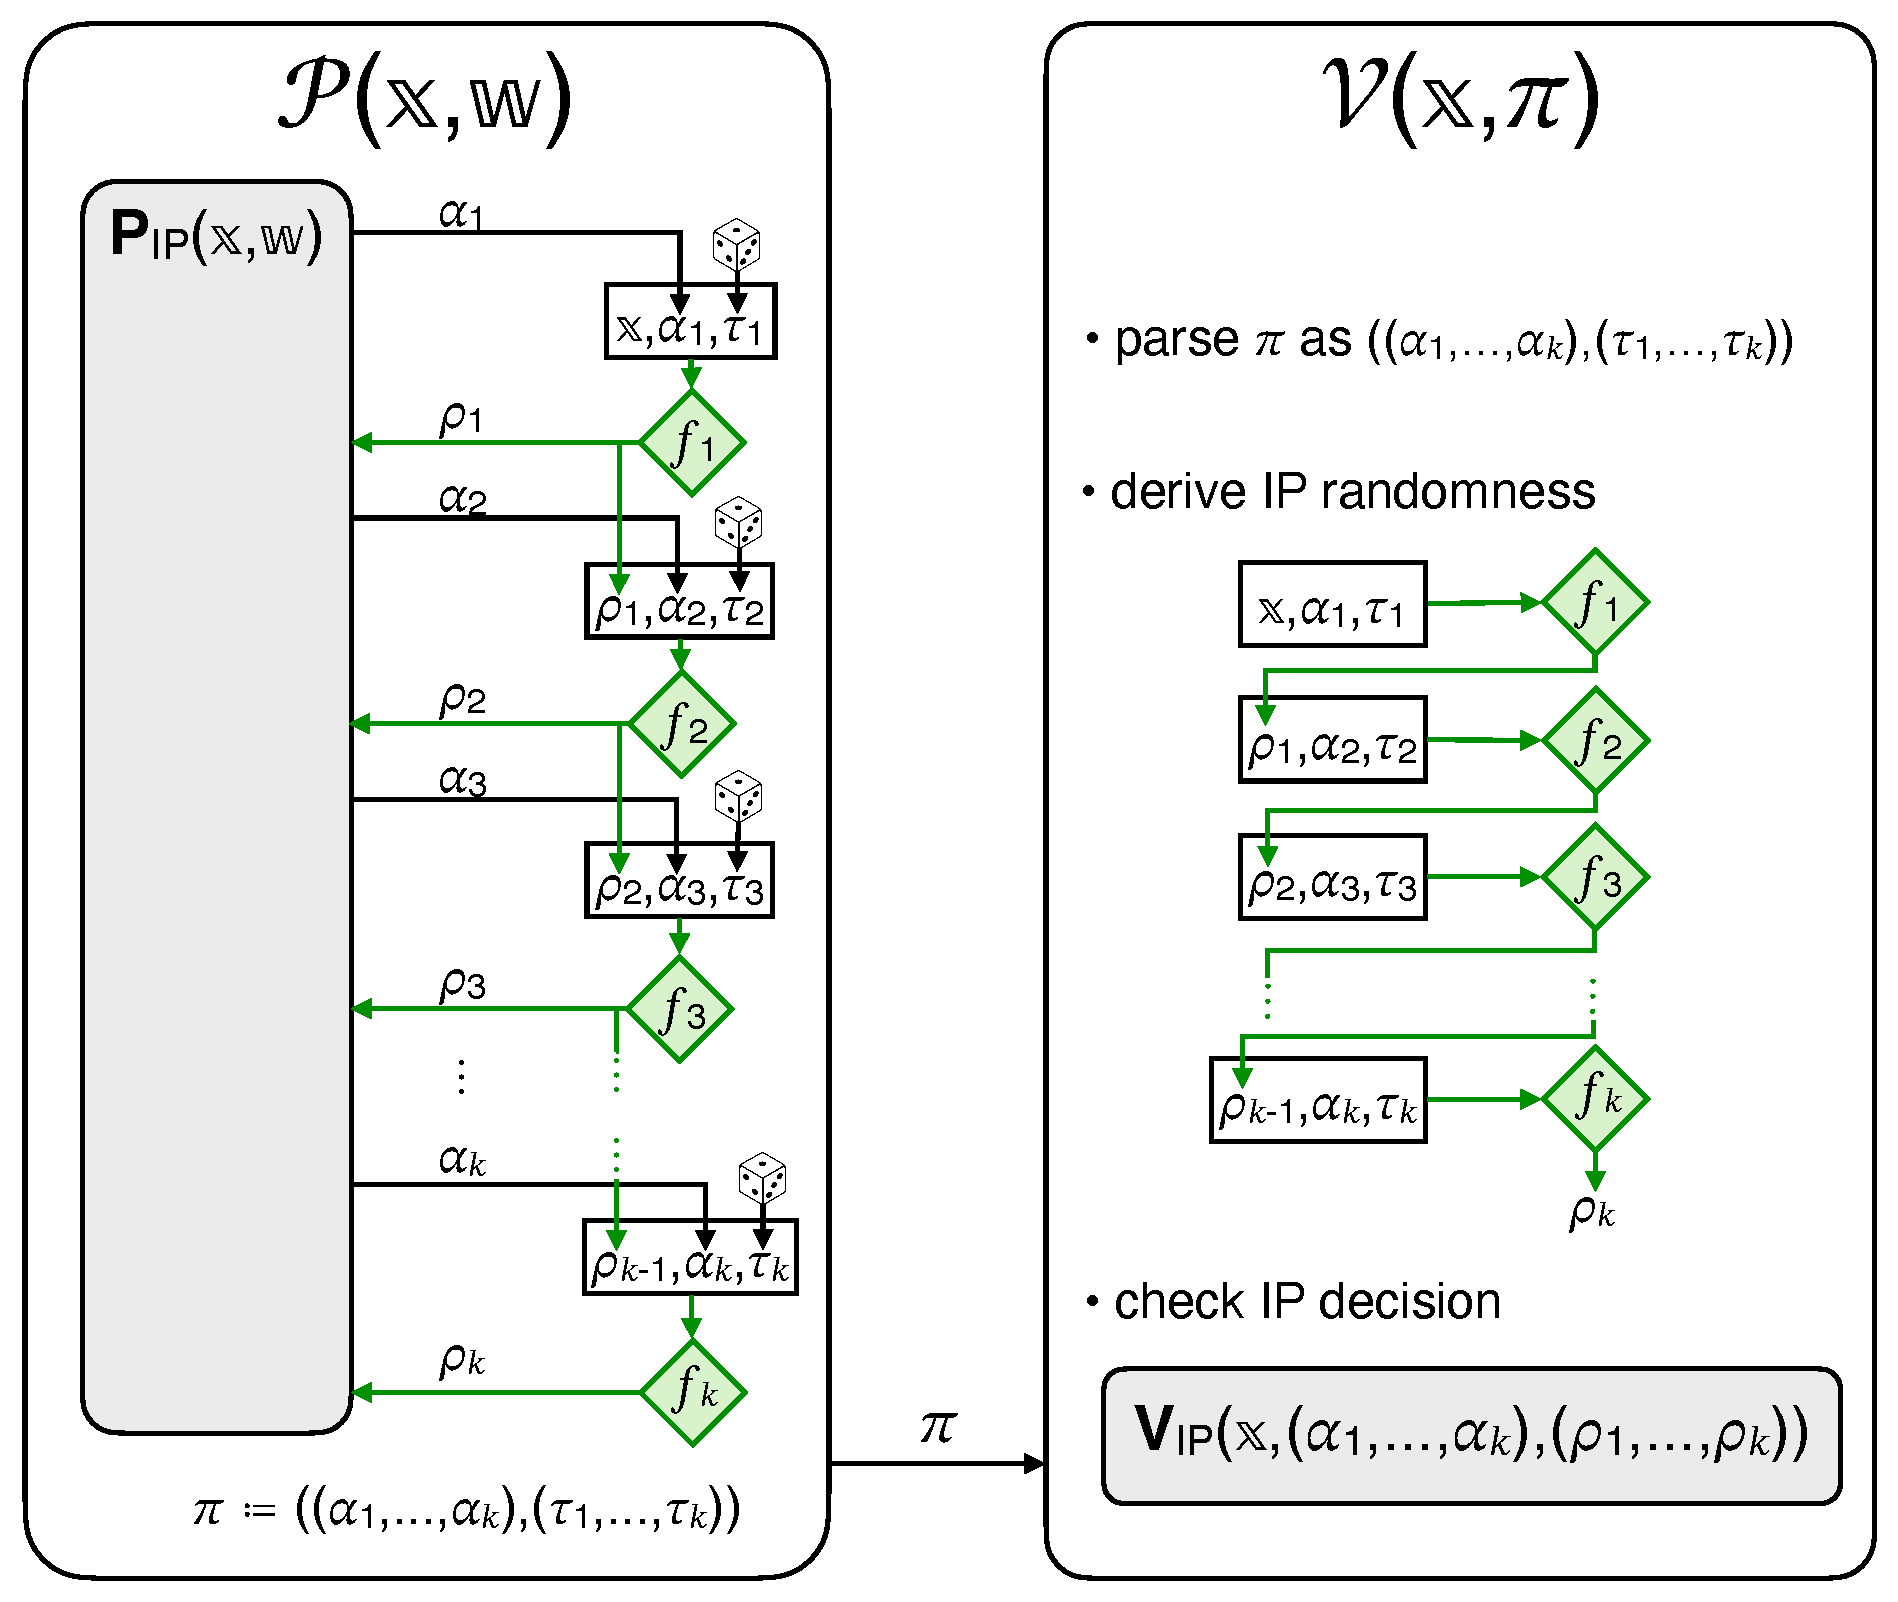
\includegraphics[width=0.8\textwidth]{\FigureFolder/fast-fs-ip-diagram}
\caption[Diagram of the fast FS transformation for public-coin IPs]{Diagram of the \FastFSonIPText ($\FastFSonIPSymbol$ in \Cref{construction:fast-fs-for-public-coin-ip}).}
\label{figure:fast-fs-for-ip-diagram}
\end{figure}

%%%%%%%%%%%%%%%%%%%%%%%%%%%%%%%%%%%%%%%%%%%%%%%%%%%%%%%%%%%%%%%%%%%%%%%%%%%%%%%
%%%%%%%%%%%%%%%%%%%%%%%%%%%%%%%%%%%%%%%%%%%%%%%%%%%%%%%%%%%%%%%%%%%%%%%%%%%%%%%
%%%%%%%%%%%%%%%%%%%%%%%%%%%%%%%%%%%%%%%%%%%%%%%%%%%%%%%%%%%%%%%%%%%%%%%%%%%%%%%
\section{Soundness}
\label{section:fast-fs-reduction}

We prove that \Cref{construction:fast-fs-for-public-coin-ip} is adaptively sound. The following theorem states that the adaptive soundness error of the non-interactive argument is upper bounded by the IP state-restoration soundness error of the underlying IP plus a small error term (which represents the probability of \DoQuote{breaking} the hash chain). In particular, a small state-restoration soundness error for the IP is \emph{sufficient} for a small soundness error for the resulting non-interactive argument.

\begin{ImportantTheorem}{}{fast-fs-for-public-coin-ip}
Let $\IPSymbol$ be a public-coin IP for a relation $\Relation$ with state-restoration soundness error $\IPSRSoundnessError$. For every security parameter $\SecurityParameter \in \Naturals$ and privacy parameter $\PrivacyParameter \in \Naturals$, $\NARGSymbol \DefineEqual \FastFSonIPTransformation{\IPSymbol}{\SecurityParameter}{\PrivacyParameter}$ in \Cref{construction:fast-fs-for-public-coin-ip} is a non-interactive argument for $\Relation$ with adaptive soundness error $\ARGSoundnessError$ (see \Cref{definition:narg-adaptive-soundness-with-cnf}) such that
\begin{equation*}
\ARGSoundnessError(\SecurityParameter,\ROQueryBound,\InstanceSize)
\leq
\FSIPSoundnessExpression
\enspace.
\end{equation*}
\end{ImportantTheorem}

\begin{proof}
We reduce the soundness of \Cref{construction:fast-fs-for-public-coin-ip} to the soundness of \Cref{construction:slow-fs-for-public-coin-ip}. We show that every malicious argument prover for \Cref{construction:fast-fs-for-public-coin-ip} can be translated to a malicious argument prover for \Cref{construction:slow-fs-for-public-coin-ip} that wins with almost the same probability.

Denote by $\ARGVerifier_{\FastFSSymbol}$ the argument verifier in \Cref{construction:fast-fs-for-public-coin-ip} and by $\ARGVerifier_{\SlowFSSymbol}$ the argument verifier in \Cref{construction:slow-fs-for-public-coin-ip}. Fix a query bound $\ROQueryBound \in \Naturals$, $\ROQueryBound$-query argument prover $\FastFSMaliciousProver$, and instance size bound $\InstanceSize \in \Naturals$. We construct an argument prover $\SlowFSMaliciousProver$ that, using $\FastFSMaliciousProver$ as a black box, convinces $\ARGVerifier_{\SlowFSSymbol}$ with almost the same probability as $\FastFSMaliciousProver$ convinces $\ARGVerifier_{\FastFSSymbol}$ (on the same instances). Specifically, see \Cref{construction:fast-fs-malicious-prover} and \Cref{lemma:slow-vs-fast:stat-distance}, which directly implies the theorem.

This requires some effort. The construction of $\SlowFSMaliciousProver$ relies on a procedure $\FastFSMappingOracle$ (\DoQuote{fast to slow}) that translates queries of $\FastFSMaliciousProver$ to queries of $\SlowFSMaliciousProver$. In turn, $\FastFSMappingOracle$ relies on a subroutine $\FSTranscriptExtractor$, which receives as input a round index, an IP verifier challenge $\IPVerifierRandomMessage$, and a trace $\ROTrace$, and outputs the unique hash chain in $\ROTrace$ that ends in $\IPVerifierRandomMessage$ (aborting if $\ROTrace$ contains no such hash chain or contains multiple such hash chains). Below we define these procedures, and prove a generic claim about them. Then we return to $\SlowFSMaliciousProver$ and its analysis.
\end{proof}

\begin{definition}
\label{definition:fast-fs-chain-backtrack}
The procedure $\FSTranscriptExtractor$ is defined as follows.
\begin{itemize}[noitemsep]
\item[] $\FSTranscriptExtractor(\RoundIndex,\IPVerifierRandomMessage,\ROTrace)$:
\begin{enumerate}[nolistsep]
  \item Find query-answer pairs $(\ROQuery_{1},\IPVerifierRandomMessage_{1}),\ldots,(\ROQuery_{\RoundIndex},\IPVerifierRandomMessage_{\RoundIndex})$ in the trace $\ROTrace$ such that:
  \begin{itemize}[nolistsep]
    \item $(\ROQuery_{1},\IPVerifierRandomMessage_{1})$ is a query-answer pair for the oracle $\ROFunction_{1}$ and $\ROQuery_{1}$ has the form $\FSFirstQuery$;
    \item for every $j \in \{2,\dots,\RoundIndex\}$, $(\ROQuery_{j},\IPVerifierRandomMessage_{j})$ is a query-answer pair for the oracle $\ROFunction_{j}$ and $\ROQuery_{j}$ has the form $\FastFSLaterQuery{j}$;
    \item $\IPVerifierRandomMessage_{\RoundIndex} = \IPVerifierRandomMessage$.
  \end{itemize}
  \item Abort if no such list exists or if at least two such lists exist (of any lengths).
  \item Output $\SlowFSLaterQuery{\RoundIndex}$.
\end{enumerate}
\end{itemize}
If the query-answer trace $\ROTrace$ is sorted lexicographically by answer (and then by query), then $\FSTranscriptExtractor$ involves $\RoundIndex$ lookups each taking time $O(\IPMaxRandomnessComplexity \cdot \log \ROQueryBound)$, for a total running time of $O(\RoundIndex \cdot \IPMaxRandomnessComplexity \cdot \log \ROQueryBound)$. If $\ROTrace$ is not sorted then $\FSTranscriptExtractor$ first sorts $\ROTrace$ in time $O(\IPMaxRandomnessComplexity \cdot \ROQueryBound \cdot \log \ROQueryBound)$ and then performs the $\RoundIndex$ lookups, for a total running time of $O(\IPMaxRandomnessComplexity \cdot (\ROQueryBound+\RoundIndex) \cdot \log \ROQueryBound) = O(\IPMaxRandomnessComplexity \cdot (\ROQueryBound+\IPRoundComplexity) \cdot \log \ROQueryBound)$.
\end{definition}

\begin{construction}
\label{fast-fs:def-mapping-oracle}
The procedure $\FastFSMappingOracle$ receives query access to random oracles $\ROFunction = \IPTuple{\ROFunction}$ and black-box access to an algorithm $\ROAdversary$, an input $a$, and works as follows.
\begin{itemize}[noitemsep]
\item[] $\FastFSMappingOracle^{\ROFunction}(\BlackBox{\ROAdversary})(a)$:
\begin{enumerate}[noitemsep]
  \item For every $\RoundIndex \in [\IPRoundComplexity]$, lazily sample an oracle $\LazySub{\ROFunctionAlt}{\RoundIndex} \gets \RODistribution{\IPRandomnessComplexity_{\RoundIndex}}$ (to answer malformed queries).
  \item Set $\ROTrace_{\FastFSSymbol}$ to be an empty query-answer trace.
  \item Simulate $\ROAdversary(a)$ while answering a query $\ROQuery$ to the $\RoundIndex$-th oracle $\ROFunction_{\RoundIndex}$:
  \begin{enumerate}[nolistsep]
    \item If $\RoundIndex=1$ and $\ROQuery$ has the form $\FSFirstQuery$:
    \begin{enumerate}[nolistsep]
      \item answer with $\ROAnswer \DefineEqual \ROFunction_{1}(\ROQuery)$;
      \item add $(\ROQuery,\ROAnswer)$ to $\ROTrace_{\FastFSSymbol}$ as a query to oracle $\ROFunction_{1}$.
    \end{enumerate}
    \item If $\RoundIndex>1$ and $\ROQuery$ has the form $\FastFSLaterQuery{\RoundIndex}$:
    \begin{enumerate}[nolistsep]
      \item run $\SlowFSLaterQuery{\RoundIndex-1} \DefineEqual \FSTranscriptExtractor(\RoundIndex-1, \IPVerifierRandomMessage_{\RoundIndex-1}, \ROTrace_{\FastFSSymbol})$;
      \item if $\FSTranscriptExtractor$ aborted then answer with $\LazySub{\ROFunctionAlt}{\RoundIndex}(\ROQuery)$;
      \item otherwise answer with $\ROAnswer \DefineEqual \ROFunction_{\RoundIndex}\SlowFSLaterQuery{\RoundIndex}$, and add $(\ROQuery,\ROAnswer)$ to $\ROTrace_{\FastFSSymbol}$ as a query to oracle $\ROFunction_{\RoundIndex}$.
    \end{enumerate}
    \item Else answer with $\LazySub{\ROFunctionAlt}{\RoundIndex}(\ROQuery)$.
  \end{enumerate}
  \item Once $\ROAdversary$ halts with outputs $b$, output $b$.
\end{enumerate}
\end{itemize}
We use $b \xgetsbelow{\ROTrace_{\FastFSSymbol}} \FastFSMappingOracle^{\ROFunction}(\ROAdversary)$ to denote the internal variable $\ROTrace_{\FastFSSymbol}$ at the end of the execution of $\ROAdversary$; note that $\ROTrace_{\FastFSSymbol}$ is not the query-answer trace of $\ROAdversary$ to $\ROFunction$.

If $\ROAdversary$ makes at most $\ROQueryBound$ queries to $\ROFunction=\IPTuple{\ROFunction}$ then $\FastFSMappingOracle(\ROAdversary)$ makes at most $\ROQueryBound$ queries to $\ROFunction=\IPTuple{\ROFunction}$. Moreover, the running time of $\FastFSMappingOracle(\ROAdversary)$ equals the running time of $\ROAdversary$ plus $O(\IPMaxRandomnessComplexity \cdot \IPRoundComplexity \cdot \ROQueryBound \cdot \log \ROQueryBound)$. Indeed, $\FastFSMappingOracle$ runs $\ROAdversary$ and answers each of its $\ROQueryBound$ queries following a certain procedure. The time to answer a query is dominated by the time to run $\FSTranscriptExtractor$, which is at most $O(\IPRoundComplexity \cdot \IPMaxRandomnessComplexity \cdot \log \ROQueryBound)$ provided that $\ROTrace_{\FastFSSymbol}$ is sorted; this amounts to $\ROQueryBound \cdot O(\IPRoundComplexity \cdot \IPMaxRandomnessComplexity \cdot \log \ROQueryBound)$ total work across all $\ROQueryBound$ queries. Separately, ensuring that $\ROTrace_{\FastFSSymbol}$ is always sorted takes time $O(\IPMaxRandomnessComplexity \cdot \ROQueryBound \cdot \log \ROQueryBound)$ across all $\ROQueryBound$ queries.
\end{construction}



\begin{construction}
\label{construction:fast-trace-to-slow-trace}
The function $\FastTraceToSlowTrace$ receives as input a query-answer trace $\ROTrace_{\FastFSSymbol}$ of length $\ROQueryBound$ and outputs a query-answer trace $\ROTrace_{\SlowFSSymbol}$, and works as follows.
\begin{itemize}[noitemsep]
\item[] $\FastTraceToSlowTrace(\ROTrace_{\FastFSSymbol})$:
\begin{enumerate}[nolistsep]
  \item Initialize an empty query-answer trace $\ROTrace_{\SlowFSSymbol}$.
  \item For $\ROQueryIndex = 1,\dots,\ROQueryBound$:
  \begin{enumerate}[nolistsep]
    \item Let $(\ROQuery,\ROAnswer)$ be the $\ROQueryIndex$-th query-answer pair in $\ROTrace_{\FastFSSymbol}$, and let it be to the $\RoundIndex$-th oracle.
    \item If $\RoundIndex=1$ then add $(\ROQuery,\ROAnswer)$ to $\ROTrace_{\SlowFSSymbol}$ as a query-answer pair for $\ROFunction_{1}$.
    \item If $\RoundIndex \in \{2,\dots,\IPRoundComplexity\}$ and $\ROQuery$ has the form $\FastFSLaterQuery{\RoundIndex}$ then:
    \begin{enumerate}[nolistsep]
      \item run $\SlowFSLaterQuery{\RoundIndex-1} \DefineEqual \FSTranscriptExtractor(\RoundIndex-1, \IPVerifierRandomMessage_{\RoundIndex-1}, \ROTrace_{\FastFSSymbol})$;
      \item if $\FSTranscriptExtractor$ did not abort then add $\big(\SlowFSLaterQuery{\RoundIndex-1},\ROAnswer\big)$ to $\ROTrace_{\SlowFSSymbol}$ as a query-answer pair for $\ROFunction_{\RoundIndex}$.
    \end{enumerate}
  \end{enumerate}
  \item Output $\ROTrace_{\SlowFSSymbol}$.
\end{enumerate}
\end{itemize}
The function $\FastTraceToSlowTrace$ can be computed in time $\FastTraceToSlowTraceTime$ by sorting $\ROTrace_{\FastFSSymbol}$ (by answer and then by query) and then, inside the main loop, searching from each previous element in the sequence one by one.
\end{construction}

We prove a generic claim about $\FastFSMappingOracle$ (\Cref{fast-fs:def-mapping-oracle}) and $\FastTraceToSlowTrace$ (\Cref{construction:fast-trace-to-slow-trace}). We define two events based on a query-answer trace, and then the union of the two events:
\begin{enumerate}[noitemsep]
  \item $\CollisionEvent(\ROTrace_{\FastFSSymbol})$ is the event that $\ROTrace_{\FastFSSymbol}$ contains a collision on the same oracle (i.e., there exists $\RoundIndex \in [\IPRoundComplexity]$ such that $\ROTrace_{\FastFSSymbol}$ contains two distinct queries to the oracle $\ROFunction_{\RoundIndex}$ with the same answer);
  \item $\InversionEvent(\ROTrace_{\FastFSSymbol})$ is the event that there exist $\ROQueryIndex_{1}, \ROQueryIndex_{2} \in [\ROQueryBound]$ with $\ROQueryIndex_{1} < \ROQueryIndex_{2}$ and $\RoundIndex \in \{2,\dots,\IPRoundComplexity\}$ such that the $\ROQueryIndex_{1}$-th query in $\ROTrace_{\FastFSSymbol}$ is to oracle $\ROFunction_{\RoundIndex}$ and has the form $\FastFSLaterQuery{\RoundIndex}$ and the $\ROQueryIndex_{2}$-th answer in $\ROTrace_{\FastFSSymbol}$ is to the oracle $\ROFunction_{\RoundIndex-1}$ and has the answer $\IPVerifierRandomMessage_{\RoundIndex-1}$.
  \item $\Event(\ROTrace_{\FastFSSymbol}) \DefineEqual \CollisionEvent(\ROTrace_{\FastFSSymbol}) \lor \InversionEvent(\ROTrace_{\FastFSSymbol})$.
\end{enumerate}

\begin{claim}
\label{fast-fs:claim-fast-to-slow-conditioned}
For every algorithm $\ROAdversary$ the following two distributions are identical:
\begin{align*}
&\left\{
\begin{array}{l}
  (\ROTrace_{\SlowFSSymbol},y) \\
  \ConditionedOnText \\
  \Negate{\Event(\ROTrace)}
\end{array}
\GivenExperiment
\StateExperiment{
  \ROFunction \gets \RODistribution{\IPTuple{\IPRandomnessComplexity}} \\
  y \xleftarrow{\ROTrace} \ROAdversary^{\ROFunction} \\
  \ROTrace_{\SlowFSSymbol} \gets \FastTraceToSlowTrace(\ROTrace)
}
\right\}
\\ & \equiv
\left\{
\begin{array}{l}
  (\ROTrace,y) \\
  \ConditionedOnText \\
  \Negate{\Event(\ROTrace_{\FastFSSymbol})}
\end{array}
\GivenExperiment
\StateExperiment{
  \ROFunction \gets \RODistribution{\IPTuple{\IPRandomnessComplexity}} \\
  y \xleftarrow[\ROTrace_{\FastFSSymbol}]{\ROTrace} \FastFSMappingOracle^{\ROFunction}(\ROAdversary)
}
\right\}
\enspace.
\end{align*}
Above, $\ROTrace_{\FastFSSymbol}$ in the right-side experiment is the query-answer trace internally maintained by $\FastFSMappingOracle$, and $\ROTrace$ is the query-answer trace to $\ROFunction$. Moreover, $\Pr[\Event(\ROTrace)] =  \Pr[\Event(\ROTrace_{\FastFSSymbol})]$.
\end{claim}

\begin{proof}
We show that the distribution of query answers given to $\ROAdversary$ in both experiments are identical. Then we discuss the distributions of $(\ROTrace_{\SlowFSSymbol},y)$ and $(\ROTrace,y)$.

We separately consider the case of duplicate queries and new queries. Below, for every $\ROQueryIndex \in [\ROQueryBound]$, we let $\ROTrace_{\ROQueryIndex}$ be the prefix of $\ROTrace_{\FastFSSymbol}$ containing the first $\ROQueryIndex$ query-answer pairs.

\parhead{Case 1: duplicate queries}
In the left-side experiment, it is clear that duplicate queries to $\ROFunction$ are answered consistently. Next we argue that, in the right-side experiment, answers given by $\FastFSMappingOracle^{\ROFunction}$ for duplicate queries are consistent. This is evident for all queries except for queries to $\ROFunction_{\RoundIndex}$ of the form $\FastFSLaterQuery{\RoundIndex}$ for some $\RoundIndex \in \{2,\dots,\IPRoundComplexity\}$. These queries are answered via the output of $\FSTranscriptExtractor$ (if no abort) or via the lazily sampled oracles $(\LazySub{\ROFunctionAlt}{\RoundIndex})_{\RoundIndex \in [\IPRoundComplexity]}$ (if there is an abort). Duplicate queries are handled in $\FastFSMappingOracle^{\ROFunction}$ by multiple executions of $\FSTranscriptExtractor$ with the same index and input $\IPVerifierRandomMessage$ but \emph{different input traces}, which in principle might result in different answers. However, we prove that the relevant executions of $\FSTranscriptExtractor$ all have the same output (provided $\Negate{\CollisionEvent(\ROTrace_{\FastFSSymbol})} \land \Negate{\InversionEvent(\ROTrace_{\FastFSSymbol})}$ holds), using the fact that the traces for later executions are extensions of traces for earlier executions.

Assume that $\Negate{\CollisionEvent(\ROTrace_{\FastFSSymbol})} \land \Negate{\InversionEvent(\ROTrace_{\FastFSSymbol})}$ holds. Let $\ROQueryIndex_{1},\ROQueryIndex_{2} \in [\ROQueryBound]$ with $\ROQueryIndex_{1} < \ROQueryIndex_{2}$. Let $\FastFSLaterQuery{\RoundIndex}$ be the $\ROQueryIndex_{1}$-th query in $\ROTrace_{\FastFSSymbol}$ (assume it is a query to $\ROFunction_{\RoundIndex}$). We prove that
\begin{align*}
\FSTranscriptExtractor(\RoundIndex-1,\IPVerifierRandomMessage_{\RoundIndex-1},\ROTrace_{\ROQueryIndex_{1}})
= \FSTranscriptExtractor(\RoundIndex-1,\IPVerifierRandomMessage_{\RoundIndex-1},\ROTrace_{\ROQueryIndex_{2}})
\enspace,
\end{align*}
where above we assume that if $\FSTranscriptExtractor$ aborts then it outputs a special abort symbol.

Recall that $\FSTranscriptExtractor$ searches for valid sequences $(\ROQuery_{1},\IPVerifierRandomMessage_{1}),\ldots,(\ROQuery_{\RoundIndex-1},\IPVerifierRandomMessage_{\RoundIndex-1})$ of query-answer pairs in the given trace. It aborts if no valid sequence is found, or if multiple valid sequences are found. We distinguish between different cases.
\begin{itemize}[noitemsep]
  \item $\FSTranscriptExtractor(\RoundIndex-1,\IPVerifierRandomMessage_{\RoundIndex-1},\ROTrace_{\ROQueryIndex_{1}})$ aborts and $\FSTranscriptExtractor(\RoundIndex-1,\IPVerifierRandomMessage_{\RoundIndex-1},\ROTrace_{\ROQueryIndex_{2}})$ aborts. In this case, both executions output the same special abort symbol and hence have the same output.
  \item $\FSTranscriptExtractor(\RoundIndex-1,\IPVerifierRandomMessage_{\RoundIndex-1},\ROTrace_{\ROQueryIndex_{1}})$ aborts but $\FSTranscriptExtractor(\RoundIndex-1,\IPVerifierRandomMessage_{\RoundIndex-1},\ROTrace_{\ROQueryIndex_{2}})$ does not abort. This means that $\ROTrace_{\ROQueryIndex_{2}}$ contains a valid sequence but $\ROTrace_{\ROQueryIndex_{1}}$ does not contain one. However, since the query $\FastFSLaterQuery{\RoundIndex}$ was performed in $\ROTrace_{\ROQueryIndex_{1}}$ this contradicts $\Negate{\InversionEvent(\ROTrace_{\FastFSSymbol})}$.
  \item $\FSTranscriptExtractor(\RoundIndex-1,\IPVerifierRandomMessage_{\RoundIndex-1},\ROTrace_{\ROQueryIndex_{1}})$ does not abort and $\FSTranscriptExtractor(\RoundIndex-1,\IPVerifierRandomMessage_{\RoundIndex-1},\ROTrace_{\ROQueryIndex_{2}})$ aborts. This means that $\ROTrace_{\ROQueryIndex_{1}}$ contains a valid sequence, and thus also $\ROTrace_{\ROQueryIndex_{2}}$. If $\FSTranscriptExtractor(\RoundIndex-1,\IPVerifierRandomMessage_{\RoundIndex-1},\ROTrace_{\ROQueryIndex_{2}})$ aborts then it must be because more than one valid sequence exists, which contradicts $\Negate{\CollisionEvent(\ROTrace_{\FastFSSymbol})}$.
  \item $\FSTranscriptExtractor(\RoundIndex-1,\IPVerifierRandomMessage_{\RoundIndex-1},\ROTrace_{\ROQueryIndex_{1}})$ does not abort and $\FSTranscriptExtractor(\RoundIndex-1,\IPVerifierRandomMessage_{\RoundIndex-1},\ROTrace_{\ROQueryIndex_{2}})$ does not abort. This means that $\ROTrace_{\ROQueryIndex_{1}}$ contains a single valid sequence and $\ROTrace_{\ROQueryIndex_{2}}$ contains a single valid sequence. These sequences must be the same, as otherwise $\ROTrace_{\ROQueryIndex_{2}}$ would contains two sequences (as $\ROTrace_{\ROQueryIndex_{1}}$ is a prefix of $\ROTrace_{\ROQueryIndex_{2}}$), contradicting $\Negate{\CollisionEvent(\ROTrace_{\FastFSSymbol})}$ (two valid sequences would cause a collision with the same oracle). Thus, the output of $\FSTranscriptExtractor$ is the same in both cases.
\end{itemize}

\parhead{Case 2: new queries}
It is clear that on the left side each new query gets a random response conditioned on the events. We move to the right side, and argue that answers given by $\FastFSMappingOracle^{\ROFunction}$ to \emph{new} query $\ROQuery$ (a query that was not previously issued) are uniformly random, conditioned on the event. Suppose that $\ROQuery$ is the $\ROQueryIndex$-th query. There are several cases.
\begin{itemize}[noitemsep]
  \item The query is to $\ROFunction_{1}$ but does not have the form $\FSFirstQuery$. In this case $\FastFSMappingOracle^{\ROFunction}$ answers with $\LazySub{\ROFunctionAlt}{1}(\ROQuery)$. Since $\ROQuery$ is a new query, $\LazySub{\ROFunctionAlt}{1}$ has not been queried at $\ROQuery$ and thus the answer $\LazySub{\ROFunctionAlt}{1}(\ROQuery)$ is uniformly random.
  \item The query is to $\ROFunction_{1}$ and has the form $\FSFirstQuery$. In this case $\FastFSMappingOracle^{\ROFunction}$ answers with $\ROFunction_{1}(\ROQuery)$. Since $\ROQuery$ is a new query, $\ROFunction_{1}$ has not been queried at $\ROQuery$ and thus the answer $\ROFunction_{1}(\ROQuery)$ is uniformly random.
  \item The query is to $\ROFunction_{\RoundIndex}$ (for $1 < \RoundIndex \leq \IPRoundComplexity$) but does not have the form $\FastFSLaterQuery{\RoundIndex}$. In this case $\FastFSMappingOracle^{\ROFunction}$ answers with $\LazySub{\ROFunctionAlt}{\RoundIndex}(\ROQuery)$. Since $\ROQuery$ is a new query, $\LazySub{\ROFunctionAlt}{\RoundIndex}$ has not been queried at $\ROQuery$ and thus the answer $\LazySub{\ROFunctionAlt}{\RoundIndex}(\ROQuery)$ is uniformly random.
  \item The query is to $\ROFunction_{\RoundIndex}$ (for $1 < \RoundIndex \leq \IPRoundComplexity$), has the form $\FastFSLaterQuery{\RoundIndex}$, but $\FSTranscriptExtractor$ aborts. In this case $\FastFSMappingOracle^{\ROFunction}$ answers with $\LazySub{\ROFunctionAlt}{\RoundIndex}(\ROQuery)$. Since $\ROQuery$ is a new query, $\LazySub{\ROFunctionAlt}{\RoundIndex}$ has not been queried at $\ROQuery$ and thus the answer $\LazySub{\ROFunctionAlt}{\RoundIndex}(\ROQuery)$ is uniformly random.
  \item The query is to $\ROFunction_{\RoundIndex}$ (for $1 < \RoundIndex \leq \IPRoundComplexity$), has the form $\FastFSLaterQuery{\RoundIndex}$, and $\FSTranscriptExtractor$ does not abort. Denote the output of $\FSTranscriptExtractor$ as $\SlowFSLaterQuery{\RoundIndex-1}$. In this case $\FastFSMappingOracle^{\ROFunction}$ answers with $\ROFunction_{\RoundIndex}\SlowFSLaterQuery{\RoundIndex}$. Suppose, towards a contradiction, that $\SlowFSLaterQuery{\RoundIndex}$ was queried before. Hence there exists a previous query at time $\ROQueryIndex' < \ROQueryIndex$ of the form $(\IPVerifierRandomMessage'_{\RoundIndex-1},\IPProverMessage_{\RoundIndex},\RandSaltString_{\RoundIndex})$ such that
\begin{align*}
\FSTranscriptExtractor(\RoundIndex-1,\IPVerifierRandomMessage'_{\RoundIndex-1},\ROTrace_{\ROQueryIndex'})
= \FSTranscriptExtractor(\RoundIndex-1,\IPVerifierRandomMessage_{\RoundIndex-1},\ROTrace_{\ROQueryIndex})
\enspace.
\end{align*}
This implies that $\IPVerifierRandomMessage'_{\RoundIndex} = \IPVerifierRandomMessage_{\RoundIndex}$ and thus it is a duplicate query. Since we assumed that $\ROQuery$ is a new query, we deduce that the answer $\ROFunction_{\RoundIndex}\SlowFSLaterQuery{\RoundIndex}$ is uniformly random.
\end{itemize}
In both experiments the queries of $\ROAdversary$ are answered with the same distribution, so $\ROAdversary$'s output $y$ has the same distribution in both experiments. Moreover, in the left-side experiment $\ROTrace_{\SlowFSSymbol}$ is the output of $\FastTraceToSlowTrace$ applied to $\ROAdversary$'s query-answer trace, while in the right-side experiment $\ROTrace$ is the query-answer trace of $\FastFSMappingOracle(\ROAdversary)$; both $\FastTraceToSlowTrace$ and $\FastFSMappingOracle$ apply the same logic to $\ROAdversary$'s queries, and therefore produce the same trace (since $\ROAdversary$'s queries are answered with the same distribution). Overall, the distribution of $(\FastTraceToSlowTrace(\ROTrace),y)$ is identical to that of $(\ROTrace,y)$ which concludes the proof.

Moreover, the events $\Event(\ROTrace)$ and $\Event(\ROTrace_{\FastFSSymbol})$ are the same event applied to the two traces that we have shown have the same distribution. We conclude that $\Pr[\Event(\ROTrace)] = \Pr[\Event(\ROTrace_{\FastFSSymbol})]$.
\end{proof}

\begin{construction}
\label{construction:fast-fs-malicious-prover}
The argument prover $\SlowFSMaliciousProver$ receives query access to the random oracles $\ROFunction = \IPTuple{\ROFunction}$ and black-box access to the argument prover $\FastFSMaliciousProver$, and is defined as
\begin{equation*}
\SlowFSMaliciousProver^{\ROFunction}(\BlackBox{\FastFSMaliciousProver}) \DefineEqual \FastFSMappingOracle^{\ROFunction}(\BlackBox{\FastFSMaliciousProver})
\enspace.
\end{equation*}
The running time of $\SlowFSMaliciousProver$ is $\ProverRunningTime{\FastFSMaliciousProver} + O(\IPMaxRandomnessComplexity \cdot \IPRoundComplexity \cdot \ROQueryBound \cdot \log \ROQueryBound)$.
\end{construction}

\begin{lemma}
\label{lemma:slow-vs-fast:stat-distance}
The following two distributions are $\FSErrorExpression$-close in statistical distance:
\begin{align*}
\left\{
  (\DecisionBit,\Instance,\ARGString, \ROTrace_{\SlowFSSymbol})
  \GivenExperiment
\StateExperiment{
  \ROFunction \gets \RODistribution{\IPTuple{\IPRandomnessComplexity}} \\
  (\Instance,\ARGString) \xleftarrow{\ROTrace} \FastFSMaliciousProver^{\ROFunction} \\
  \DecisionBit \xleftarrow{\ROTraceVerifier} \ARGVerifier_{\FastFSSymbol}^{\ROFunction}(\Instance,\ARGString) \\
  \ROTrace_{\SlowFSSymbol} \gets \FastTraceToSlowTrace(\ROTrace \concat \ROTraceVerifier)
}
\right\}
\text{and}
\left\{
  (\DecisionBit,\Instance,\ARGString, \ROTrace \concat \ROTraceVerifier)
\GivenExperiment
\StateExperiment{
  \ROFunction \gets \RODistribution{\IPTuple{\IPRandomnessComplexity}} \\
  (\Instance,\ARGString) \xleftarrow{\ROTrace} \SlowFSMaliciousProver^{\ROFunction} \\
  \DecisionBit \xleftarrow{\ROTraceVerifier} \ARGVerifier_{\SlowFSSymbol}^{\ROFunction}(\Instance,\ARGString)
}
\right\}
\enspace.
\end{align*}
\end{lemma}

\begin{proof}
First, we upper bound the probability of the event $\Event(\ROTrace_{\FastFSSymbol}) = \CollisionEvent(\ROTrace_{\FastFSSymbol}) \lor \InversionEvent(\ROTrace_{\FastFSSymbol})$.

\begin{claim}
The following bound holds
\label{fast-fs:claim-bound-events}
\begin{align*}
\Pr\left[
\Event(\ROTrace_{\FastFSSymbol} \concat \ROTraceVerifierFast)
\GivenExperiment
\StateExperiment{
  \ROFunction \gets \RODistribution{\IPTuple{\IPRandomnessComplexity}} \\
  (\Instance,\ARGString) \xleftarrow[\ROTrace_{\FastFSSymbol}]{\ROTrace} \FastFSMappingOracle^{\ROFunction}(\FastFSMaliciousProver) \\
  \DecisionBit \xleftarrow[\ROTraceVerifierFast]{\ROTraceVerifier} \FastFSMappingOracle^{\ROFunction}(\ARGVerifier_{\FastFSSymbol}(\Instance,\ARGString))
}
\right]
\leq
\frac{\ROQueryBound^2}{2^{\SecurityParameter}}
\enspace.
\end{align*}
\end{claim}

\begin{proof}
Let $I_{\RoundIndex}$ be the indices of queries to oracle $\ROFunction_{\RoundIndex}$ in $\ROTrace_{\FastFSSymbol}$, and let $\ROQueryBound_{\RoundIndex} \DefineEqual \Cardinality{I_{\RoundIndex}}$; also let $\ROQueryBound_{0} \DefineEqual 0$. Note that $\sum_{\RoundIndex \in [\IPRoundComplexity]}\ROQueryBound_{\RoundIndex} \leq \ROQueryBound + \IPRoundComplexity$, because each simulated query of $\FastFSMaliciousProver$ (which makes at most $\ROQueryBound$ queries) adds at most one query to $\ROTrace_{\FastFSSymbol}$, and each simulated query of $\ARGVerifier_{\FastFSSymbol}$ (which makes $\IPRoundComplexity$ queries) adds at most one query to $\ROTrace_{\FastFSSymbol}$. Also, $\ROQueryBound_{\RoundIndex} \leq \ROQueryBound + 1$ for every $\RoundIndex \in [\IPRoundComplexity]$ because $\ARGVerifier_{\FastFSSymbol}$ makes one query to each oracle.

For every $\ROQueryIndex \in [\ROQueryBound + \IPRoundComplexity]$, let $\ROTrace_{\ROQueryIndex}$ the prefix of $\ROTrace_{\FastFSSymbol}$ of length $\ROQueryIndex$. We upper bound the probability that the $\ROQueryIndex$-th query causes the first collision or inversion: we upper bound the probability of the event $\Event(\ROTrace_{\ROQueryIndex})$ conditioned on $\Negate{\Event(\ROTrace_{\ROQueryIndex-1})}$. Let $\ROAdversary_{\ROQueryIndex}$ be the algorithm that performs the first $\ROQueryIndex-1$ queries of $\ROAdversary$ and then outputs the $\ROQueryIndex$-th query $\ROQuery_{\ROQueryIndex}$. By \Cref{fast-fs:claim-fast-to-slow-conditioned} applied to $\ROAdversary_{\ROQueryIndex}$, the answer to $\ROQuery_{\ROQueryIndex}$ from $\FastFSMappingOracle^{\ROFunction}$ is uniformly random. This lets us derive the following two bounds.
\begin{itemize}

  \item Let $\CollisionEvent^{\ROQueryIndex}$ be the event that the $\ROQueryIndex$-th query causes a collision. Suppose that $\Event(\ROTrace_{\ROQueryIndex-1})$ does not hold, and suppose that the $\ROQueryIndex$-th query is to oracle $\ROFunction_{\RoundIndex}$. Fix any previous query to oracle $\ROFunction_{\RoundIndex}$; the probability that the $\ROQueryIndex$-th query has the same answer is at most $\frac{1}{2^{\IPRandomnessComplexity_{\RoundIndex}}} \leq \frac{1}{2^{\SecurityParameter}}$. Letting $\ROQueryBound_{\RoundIndex,\ROQueryIndex}$ be the number of queries to $\ROFunction_{\RoundIndex}$ before the $\ROQueryIndex$-th query, we deduce that $\Pr\left[\CollisionEvent^{\ROQueryIndex} \ConditionedOn \Negate{\Event(\ROTrace_{\ROQueryIndex-1})}\right] \leq \frac{\ROQueryBound_{\RoundIndex,\ROQueryIndex}}{2^{\SecurityParameter}}$.

Let $\RoundIndex(\ROQueryIndex) \in [\IPRoundComplexity]$ be the index such that the $\ROQueryIndex$-th query is to oracle $\ROFunction_{\RoundIndex(\ROQueryIndex)}$. Then
\begin{align*}
\sum_{\ROQueryIndex \in [\ROQueryBound + \IPRoundComplexity]}\Pr\left[\CollisionEvent^{\ROQueryIndex} \ConditionedOn \Negate{\Event(\ROTrace_{\ROQueryIndex-1})}\right]
 \leq
\sum_{\ROQueryIndex \in [\ROQueryBound + \IPRoundComplexity]} \frac{\ROQueryBound_{\RoundIndex(\ROQueryIndex),\ROQueryIndex}}{2^{\SecurityParameter}}
 =
\sum_{\RoundIndex \in [\IPRoundComplexity]}
\sum_{\ell = 1}^{\ROQueryBound_{\RoundIndex}}
\frac{\ell}{2^{\SecurityParameter}}
 \leq
\sum_{\RoundIndex \in [\IPRoundComplexity]}
\frac{1}{2} \cdot \frac{\ROQueryBound_{\RoundIndex}^{2}}{2^{\SecurityParameter}}
\enspace.
\end{align*}


  \item Let $\InversionEvent^{\ROQueryIndex}$ be the event that the $\ROQueryIndex$-th query causes an inversion, i.e., there exists $\ROQueryIndex' \in \{1,\dots,\ROQueryIndex-1\}$ such that:
\begin{inparaenum}[(i)]
  \item the $\ROQueryIndex'$-th query is to $\ROFunction_{\RoundIndex}$ and has the form $\FastFSLaterQuery{\RoundIndex}$; and
  \item the $\ROQueryIndex$-th query, denoted by $\ROQuery_{\ROQueryIndex}$, is to oracle $\ROFunction_{\RoundIndex-1}$, does not equal any prior query, and has the answer $\ROFunction_{\RoundIndex-1}(\ROQuery_{\ROQueryIndex}) = \IPVerifierRandomMessage_{\RoundIndex-1}$.
\end{inparaenum}
Since the answer to $\ROQuery_{\ROQueryIndex}$ is random (as $\Event(\ROTrace_{\ROQueryIndex-1})$ does not hold), the probability that $\ROQuery_{\ROQueryIndex}$ causes an inversion is $\Pr\left[\ROFunction_{\RoundIndex-1}(\ROQuery_{\ROQueryIndex}) = \IPVerifierRandomMessage_{\RoundIndex-1} \ConditionedOn \Negate{\Event(\ROTrace_{\ROQueryIndex-1})}\right] = \frac{1}{2^{\IPRandomnessComplexity_{\RoundIndex-1}}} \leq \frac{1}{2^{\SecurityParameter}}$.

This lets us derive the following bound:
\begin{align*}
\sum_{\ROQueryIndex \in [\ROQueryBound + \IPRoundComplexity]} \Pr\left[\InversionEvent^{\ROQueryIndex} \ConditionedOn \Negate{\Event(\ROTrace_{\ROQueryIndex-1})}\right]
 & \leq
\sum_{i = 2}^{\IPRoundComplexity} \;
\sum_{\ROQueryIndex \in I_{\RoundIndex-1}, \ROQueryIndex' \in I_{\RoundIndex}}
\Pr\left[\ROFunction_{\RoundIndex-1}(\ROQuery_{\ROQueryIndex}) = \IPVerifierRandomMessage_{\RoundIndex-1} \ConditionedOn \Negate{\Event(\ROTrace_{\ROQueryIndex-1})}\right]
\\ & \leq
\sum_{i = 2}^{\IPRoundComplexity} \;
\sum_{\ROQueryIndex \in I_{\RoundIndex-1}, \ROQueryIndex' \in I_{\RoundIndex}}
 \frac{1}{2^{\SecurityParameter}}
\\ & =
\sum_{i = 2}^{\IPRoundComplexity}
\frac{\ROQueryBound_{\RoundIndex-1} \cdot \ROQueryBound_{\RoundIndex}}{2^{\SecurityParameter}}
\enspace.
\end{align*}
\end{itemize}
Together, we conclude the following upper bound for the probability of $\Event(\ROTrace_{\FastFSSymbol})$:
\begin{align*}
\Pr[\Event(\ROTrace_{\FastFSSymbol})]
& = \Pr[\CollisionEvent(\ROTrace_{\FastFSSymbol}) \lor \InversionEvent(\ROTrace_{\FastFSSymbol})] \\
& \leq
\sum_{\ROQueryIndex \in [\ROQueryBound + \IPRoundComplexity]}
\Pr\left[\CollisionEvent^{\ROQueryIndex}(\ROTrace_{\FastFSSymbol}) \lor \InversionEvent^{\ROQueryIndex}(\ROTrace_{\FastFSSymbol}) \ConditionedOn \Negate{\Event(\ROTrace_{\ROQueryIndex-1})}\right]
\\ & \leq
\sum_{\ROQueryIndex \in [\ROQueryBound + \IPRoundComplexity]}
\Pr\left[\CollisionEvent^{\ROQueryIndex}(\ROTrace_{\FastFSSymbol}) \ConditionedOn \Negate{\Event(\ROTrace_{\ROQueryIndex-1})}\right]
+
\Pr\left[\InversionEvent^{\ROQueryIndex}(\ROTrace_{\FastFSSymbol}) \ConditionedOn \Negate{\Event(\ROTrace_{\ROQueryIndex-1})}\right]
\\ & \leq
\frac{1}{2^{\SecurityParameter}} \cdot
\left(
\sum_{\RoundIndex \in [\IPRoundComplexity]}
\frac{\ROQueryBound_{\RoundIndex}^2}{2} +
\sum_{\RoundIndex=2}^{\IPRoundComplexity}
\ROQueryBound_{\RoundIndex-1} \cdot \ROQueryBound_{\RoundIndex}
\right)
\\ & \leq
\frac{1}{2^{\SecurityParameter}} \cdot
\left(
\frac{(\ROQueryBound+1)^2}{2} +
\frac{(\ROQueryBound+1)^2}{4}
\right)
\\ & \leq
\frac{\ROQueryBound^2}{2^{\SecurityParameter}}
\enspace.
\end{align*}
In the second to last inequality above, we use the upper bound $\sum_{\RoundIndex \in [\IPRoundComplexity]}
\frac{\ROQueryBound_{\RoundIndex}^2}{2} \leq \frac{(\ROQueryBound+1)^2}{2}$ since the maximum is attained when $\ROQueryBound_{i}=\ROQueryBound+1$ for some $\RoundIndex \in [\IPRoundComplexity]$, and we use the upper bound $\sum_{\RoundIndex \in [\IPRoundComplexity]}
\ROQueryBound_{\RoundIndex-1} \cdot \ROQueryBound_{\RoundIndex} \leq \frac{(\ROQueryBound+1)^2}{4}$ implied by \Cref{lemma:sum-seq-prod} (by setting $\delta_{\RoundIndex} \DefineEqual \frac{\ROQueryBound_{\RoundIndex}}{\ROQueryBound+1}$). The last inequality holds for every $\ROQueryBound \geq 7$.


\end{proof}

Next, we relate the execution of $\ARGVerifier_{\SlowFSSymbol}^{\ROFunction}(\Instance,\ARGString)=1$ to the execution of $\FastFSMappingOracle^{\ROFunction}(\ARGVerifier_{\FastFSSymbol})(\Instance,\ARGString)=1$.

\begin{claim}
\label{fast-fs:claim-fast-slow-g}
The following two distributions are equivalent:
\begin{align*}
& \left\{
\begin{array}{l}
  (\DecisionBit,\Instance,\ARGString,\ROTrace \concat \ROTraceVerifier) \\
  \ConditionedOnText \\
  \Negate{\Event(\ROTrace_{\FastFSSymbol} \concat \ROTraceVerifierFast)}
\end{array}
\GivenExperiment
\StateExperiment{
  \ROFunction \gets \RODistribution{\IPTuple{\IPRandomnessComplexity}} \\
  (\Instance,\ARGString) \xleftarrow[\ROTrace_{\FastFSSymbol}]{\ROTrace} \SlowFSMaliciousProver^{\ROFunction} \\
  \DecisionBit \xleftarrow[\ROTraceVerifierFast]{\ROTraceVerifier} \FastFSMappingOracle^{\ROFunction}(\ARGVerifier_{\FastFSSymbol})(\Instance,\ARGString)
}
\right\}
\\ &\equiv
\left\{
\begin{array}{l}
  (\DecisionBit,\Instance,\ARGString,\ROTrace \concat \ROTraceVerifier) \\
  \ConditionedOnText \\
  \Negate{\Event(\ROTrace_{\FastFSSymbol} \concat \ROTraceVerifierFast)}
\end{array}
\GivenExperiment
\StateExperiment{
  \ROFunction \gets \RODistribution{\IPTuple{\IPRandomnessComplexity}} \\
  (\Instance,\ARGString) \xleftarrow[\ROTrace_{\FastFSSymbol}]{\ROTrace} \SlowFSMaliciousProver^{\ROFunction} \\
  \DecisionBit \xleftarrow{\ROTraceVerifier} \ARGVerifier_{\SlowFSSymbol}^{\ROFunction}(\Instance,\ARGString) \\
  \DecisionBit' \xleftarrow[\ROTraceVerifierFast]{\ROTraceVerifier'} \FastFSMappingOracle^{\ROFunction}(\ARGVerifier_{\FastFSSymbol})(\Instance,\ARGString)
}
\right\}
\enspace.
\end{align*}
\end{claim}

\begin{proof}
The analysis below relies only on the fact that the event $\CollisionEvent(\ROTrace_{\FastFSSymbol})$ does not hold; the claim statement includes the condition that the event $\InversionEvent(\ROTrace_{\FastFSSymbol})$ does not hold only to simplify how the claim is invoked later on. Let $(\Instance,\ARGString)$ be the output of $\SlowFSMaliciousProver$, where $\ARGString = \FSARGString$.

On the right side, $\ARGVerifier_{\SlowFSSymbol}^{\ROFunction}(\Instance,\ARGString)=1$ if and only if $\IPVerifier\big(\IPVerifierInput\big)=1$ where
\begin{align*}
\forall\,\RoundIndex \in [\IPRoundComplexity]\,,\;
\IPVerifierRandomMessage_{\RoundIndex} = \ROFunction_{\RoundIndex}\SlowFSLaterQuery{\RoundIndex}
\enspace.
\end{align*}
On the left side, $\FastFSMappingOracle^{\ROFunction}(\ARGVerifier_{\FastFSSymbol}(\Instance,\ARGString))=1$ if and only if $\IPVerifier\big(\Instance,\IPTuple{\IPProverMessage},\IPTuple{\IPVerifierRandomMessage'}\big)=1$ where $\IPVerifierRandomMessage'_{\RoundIndex}$ is derived by the $\FastFSMappingOracle^{\ROFunction}$ algorithm. We show that $\IPVerifierRandomMessage'_{\RoundIndex} = \IPVerifierRandomMessage_{\RoundIndex}$ for every $\RoundIndex \in [\IPRoundComplexity]$.

The case where $\RoundIndex=1$ holds straightforwardly because
\begin{align*}
\IPVerifierRandomMessage'_{1}
= \ROFunction_{1}\FSFirstQuery = \IPVerifierRandomMessage_{1}
\enspace.
\end{align*}

We continue to the case where $\RoundIndex=2$. The randomness $\IPVerifierRandomMessage'_{2}$ is derived as follows. The algorithm $\FastFSMappingOracle^{\ROFunction}_{2}$, on input $(\IPVerifierRandomMessage_{1},\IPProverMessage_{2},\RandSaltString_{2})$, runs $\FSTranscriptExtractor(1,\IPVerifierRandomMessage_{1},\ROTrace)$ and must obtain the output $\FSFirstQuery$; indeed, a different output would yield a collision in $\ROTrace_{\FastFSSymbol}$ (contradicting $\Negate{\CollisionEvent(\ROTrace_{\FastFSSymbol})}$). Hence, we get that $\ROFunction_{2}\big(\Instance,(\IPProverMessage_{1},\IPProverMessage_{2}),(\RandSaltString_{1},\RandSaltString_{2})\big) = \IPVerifierRandomMessage_{2}$.

This continues in a similar manner up to $\IPRoundComplexity$, which we show by induction on $\RoundIndex$. We already discussed the base case of $\RoundIndex=2$ (and also $\RoundIndex=1$). For every $\RoundIndex \in \{3,\dots,\IPRoundComplexity\}$, $\IPVerifierRandomMessage'_{\RoundIndex}$ is derived as follows. The algorithm $\FastFSMappingOracle^{\ROFunction}$, on input $\FastFSLaterQuery{\RoundIndex}$, runs $\FSTranscriptExtractor(\RoundIndex-1,\IPVerifierRandomMessage_{\RoundIndex-1},\ROTrace_{\FastFSSymbol})$. Note that $\FSTranscriptExtractor(\RoundIndex-1,\IPVerifierRandomMessage_{\RoundIndex-1},\ROTrace_{\FastFSSymbol})$ does not abort because:
\begin{inparaenum}[(i)]
  \item the trace $\ROTrace_{\FastFSSymbol}$ contains all queries of $\FastFSMappingOracle^{\ROFunction}(\ARGVerifier_{\FastFSSymbol}(\Instance,\ARGString))$, so $\FSTranscriptExtractor$ has at least one chain to backtrack to; and
  \item no other chain can exist since that would imply a collision (contradicting $\Negate{\CollisionEvent(\ROTrace_{\FastFSSymbol})}$).
\end{inparaenum}
By the induction hypothesis, $\FSTranscriptExtractor(\RoundIndex-2,\IPVerifierRandomMessage_{\RoundIndex-2},\ROTrace_{\FastFSSymbol})$ gives the output ${\big(\Instance,(\IPProverMessage_{1},\dots,\IPProverMessage_{\RoundIndex-2}),(\RandSaltString_{1},\dots,\RandSaltString_{\RoundIndex-2})\big)}$. This means that the output of $\FSTranscriptExtractor(\RoundIndex-1,\IPVerifierRandomMessage_{\RoundIndex-1},\ROTrace_{\FastFSSymbol})$ must be $\SlowFSLaterQuery{\RoundIndex-1}$, as a different output would yield a collision in $\ROTrace_{\FastFSSymbol}$. Hence, we get that $\ROFunction_{\RoundIndex}\SlowFSLaterQuery{\RoundIndex} = \IPVerifierRandomMessage_{\RoundIndex}$, which lets us conclude that
\begin{align*}
\IPVerifierRandomMessage'_{\RoundIndex}
= \ROFunction_{\RoundIndex}\SlowFSLaterQuery{\RoundIndex}
= \IPVerifierRandomMessage_{\RoundIndex}
\enspace.
\end{align*}
\end{proof}

The claims we have proven allow us to upper bound the statistical distance as follows. We begin by showing that the following two distributions are equivalent:
\begin{align*}
& \left\{
\begin{array}{l}
  (\DecisionBit,\Instance,\ARGString,\ROTrace_{\SlowFSSymbol}) \\
   \ConditionedOnText \\
  \Negate{\Event(\ROTrace \concat \ROTraceVerifier)}
\end{array}
\GivenExperiment
\StateExperiment{
  \ROFunction \gets \RODistribution{\IPTuple{\IPRandomnessComplexity}} \\
  (\Instance,\ARGString) \xleftarrow{\ROTrace} \FastFSMaliciousProver^{\ROFunction} \\
  \DecisionBit \xleftarrow{\ROTraceVerifier} \ARGVerifier_{\FastFSSymbol}^{\ROFunction}(\Instance,\ARGString)\\
  \ROTrace_{\SlowFSSymbol} \gets \FastTraceToSlowTrace(\ROTrace \concat \ROTraceVerifier)
}
\right\}
\\ & \; \text{and}\; \\ &
\left\{
\begin{array}{l}
  (\DecisionBit,\Instance,\ARGString,\ROTrace \concat \ROTraceVerifier) \\
  \ConditionedOnText \\
  \Negate{\Event(\ROTrace_{\FastFSSymbol} \concat \ROTraceVerifierFast)}
\end{array}
\GivenExperiment
\StateExperiment{
  \ROFunction \gets \RODistribution{\IPTuple{\IPRandomnessComplexity}} \\
  (\Instance,\ARGString) \xleftarrow[\ROTrace_{\FastFSSymbol}]{\ROTrace} \SlowFSMaliciousProver^{\ROFunction} \\
  \DecisionBit \xleftarrow{\ROTraceVerifier} \ARGVerifier_{\SlowFSSymbol}^{\ROFunction}(\Instance,\ARGString) \\
  \DecisionBit' \xleftarrow[\ROTraceVerifierFast]{\ROTraceVerifier'} \FastFSMappingOracle^{\ROFunction}(\ARGVerifier_{\FastFSSymbol})(\Instance,\ARGString)
}
\right\}
\enspace.
\end{align*}
Note that $\Negate{\Event(\ROTrace \concat \ROTraceVerifier)}$ implies that $\Negate{\Event(\ROTrace)}$ and $\Negate{\Event(\ROTraceVerifier)}$. Hence, by applying \Cref{fast-fs:claim-fast-to-slow-conditioned} for $\ROAdversary \DefineEqual \FastFSMaliciousProver$ the left-side distribution is equivalent to
\begin{align*}
\left\{
\begin{array}{l}
  (\DecisionBit,\Instance,\ARGString,\ROTrace \concat \ROTraceVerifierSlow) \\
  \ConditionedOnText \\
  \Negate{\Event(\ROTrace_{\FastFSSymbol} \concat \ROTraceVerifier)}
\end{array}
\GivenExperiment
\StateExperiment{
  \ROFunction \gets \RODistribution{\IPTuple{\IPRandomnessComplexity}} \\
  (\Instance,\ARGString) \xleftarrow[\ROTrace_{\FastFSSymbol}]{\ROTrace} \FastFSMappingOracle^{\ROFunction}(\FastFSMaliciousProver) \\
  \DecisionBit \xleftarrow{\ROTraceVerifier} \ARGVerifier_{\FastFSSymbol}^{\ROFunction}(\Instance,\ARGString) \\
  \ROTraceVerifierSlow \gets \FastTraceToSlowTrace(\ROTraceVerifier)
}
\right\}
\enspace;
\end{align*}
moreover, the claim tells us that $\Pr[\Event(\ROTrace \concat \ROTraceVerifier)] = \Pr[\Event(\ROTrace_{\FastFSSymbol} \concat \ROTraceVerifier)]$. Then, by applying \Cref{fast-fs:claim-fast-to-slow-conditioned} for $\ROAdversary \DefineEqual \ARGVerifier_{\FastFSSymbol}$ the last distribution is equivalent to:
\begin{align*}
\left\{
\begin{array}{l}
  (\DecisionBit,\Instance,\ARGString,\ROTrace \concat \ROTraceVerifier) \\
  \ConditionedOnText \\
  \Negate{\Event(\ROTrace_{\FastFSSymbol} \concat \ROTraceVerifierFast)}
\end{array}
\GivenExperiment
\StateExperiment{
  \ROFunction \gets \RODistribution{\IPTuple{\IPRandomnessComplexity}} \\
  (\Instance,\ARGString) \xleftarrow[\ROTrace_{\FastFSSymbol}]{\ROTrace} \FastFSMappingOracle^{\ROFunction}(\FastFSMaliciousProver) \\
  \DecisionBit \xleftarrow[\ROTraceVerifierFast]{\ROTraceVerifier} \FastFSMappingOracle^{\ROFunction}(\ARGVerifier_{\FastFSSymbol})(\Instance,\ARGString)
}
\right\}
\enspace;
\end{align*}
moreover, the claim tells us that $\Pr[\Event(\ROTrace_{\FastFSSymbol} \concat \ROTraceVerifier)] = \Pr[\Event(\ROTrace_{\FastFSSymbol} \concat \ROTraceVerifierFast)] = \Pr[\Event(\ROTrace \concat \ROTraceVerifier)]$. By the definition of $\SlowFSMaliciousProver$ (see \Cref{construction:fast-fs-malicious-prover}), the last distribution is equivalent to:
\begin{align*}
\left\{
\begin{array}{l}
  (\DecisionBit,\Instance,\ARGString,\ROTrace \concat \ROTraceVerifier) \\
  \ConditionedOnText \\
  \Negate{\Event(\ROTrace_{\FastFSSymbol} \concat \ROTraceVerifierFast)}
\end{array}
\GivenExperiment
\StateExperiment{
  \ROFunction \gets \RODistribution{\IPTuple{\IPRandomnessComplexity}} \\
  (\Instance,\ARGString) \xleftarrow[\ROTrace_{\FastFSSymbol}]{\ROTrace} \SlowFSMaliciousProver^{\ROFunction} \\
  \DecisionBit \xleftarrow[\ROTraceVerifierFast]{\ROTraceVerifier} \FastFSMappingOracle^{\ROFunction}(\ARGVerifier_{\FastFSSymbol})(\Instance,\ARGString)
}
\right\}
\enspace.
\end{align*}
Finally, by \Cref{fast-fs:claim-fast-slow-g} the last distribution is equivalent to:
\begin{align*}
\left\{
\begin{array}{l}
  (\DecisionBit,\Instance,\ARGString,\ROTrace \concat \ROTraceVerifier) \\
  \ConditionedOnText \\
  \Negate{\Event(\ROTrace_{\FastFSSymbol} \concat \ROTraceVerifierFast)}
\end{array}
\GivenExperiment
\StateExperiment{
  \ROFunction \gets \RODistribution{\IPTuple{\IPRandomnessComplexity}} \\
  (\Instance,\ARGString) \xleftarrow{\ROTrace} \SlowFSMaliciousProver^{\ROFunction} \\
  \DecisionBit \xleftarrow{\ROTraceVerifier} \ARGVerifier_{\SlowFSSymbol}^{\ROFunction}(\Instance,\ARGString) \\
  \DecisionBit' \xleftarrow{\ROTraceVerifier'} \FastFSMappingOracle^{\ROFunction}(\ARGVerifier_{\FastFSSymbol})(\Instance,\ARGString)
}
\right\}
\enspace.
\end{align*}
By \Cref{fast-fs:claim-bound-events}, we get the bound $\Pr[\Event(\ROTrace \concat \ROTraceVerifier)] \leq \FSErrorExpression$. Moreover, we have argued above that $\Pr[\Event(\ROTrace \concat \ROTraceVerifier)] = \Pr[\Event(\ROTrace_{\FastFSSymbol} \concat \ROTraceVerifierFast)]$. Thus we can apply \Cref{claim:statistical-distance-condition-event}, and obtain that:
\begin{align*}
& \StatisticalDistance{
\left\{
  (\DecisionBit,\Instance,\ARGString,\ROTrace_{\SlowFSSymbol})
\GivenExperiment
\StateExperiment{
  \ROFunction \gets \RODistribution{\IPTuple{\IPRandomnessComplexity}} \\
  (\Instance,\ARGString) \xleftarrow{\ROTrace} \FastFSMaliciousProver^{\ROFunction} \\
  \DecisionBit \xleftarrow{\ROTraceVerifier} \ARGVerifier_{\FastFSSymbol}^{\ROFunction}(\Instance,\ARGString)\\
  \ROTrace_{\SlowFSSymbol} \gets \FastTraceToSlowTrace(\ROTrace \concat \ROTraceVerifier)
}
\right\}
}
{
\left\{
(\DecisionBit,\Instance,\ARGString,\ROTrace \concat \ROTraceVerifier)
\GivenExperiment
\StateExperiment{
  \ROFunction \gets \RODistribution{\IPTuple{\IPRandomnessComplexity}} \\
  (\Instance,\ARGString) \xleftarrow{\ROTrace} \SlowFSMaliciousProver^{\ROFunction} \\
  \DecisionBit \xleftarrow{\ROTraceVerifier} \ARGVerifier_{\SlowFSSymbol}^{\ROFunction}(\Instance,\ARGString)
}
\right\}
}
\\ & \leq
\StatisticalDistanceSymbol \left(
\left\{
\begin{array}{l}
  (\DecisionBit,\Instance,\ARGString,\ROTrace_{\SlowFSSymbol}) \\
  \ConditionedOnText \\
  \Negate{\Event(\ROTrace \concat \ROTraceVerifier)}
\end{array}
\GivenExperiment
\StateExperiment{
  \ROFunction \gets \RODistribution{\IPTuple{\IPRandomnessComplexity}} \\
  (\Instance,\ARGString) \xleftarrow{\ROTrace} \FastFSMaliciousProver^{\ROFunction} \\
  \DecisionBit \xleftarrow{\ROTraceVerifier} \ARGVerifier_{\FastFSSymbol}^{\ROFunction}(\Instance,\ARGString)\\
  \LongExecution{\ROTrace_{\SlowFSSymbol}}{\FastTraceToSlowTrace(\ROTrace \concat \ROTraceVerifier)}
}
\right\} \right.
,\\ & \phantom{aaaaai}
\left.
\left\{
\begin{array}{l}
  (\DecisionBit,\Instance,\ARGString,\ROTrace \concat \ROTraceVerifier) \\
  \ConditionedOnText \\
  \Negate{\Event(\ROTrace_{\FastFSSymbol} \concat \ROTraceVerifierFast)}
\end{array}
\GivenExperiment
\StateExperiment{
  \ROFunction \gets \RODistribution{\IPTuple{\IPRandomnessComplexity}} \\
  (\Instance,\ARGString) \xleftarrow[\ROTrace_{\FastFSSymbol}]{\ROTrace} \SlowFSMaliciousProver^{\ROFunction} \\
  \DecisionBit \xleftarrow{\ROTraceVerifier} \ARGVerifier_{\SlowFSSymbol}^{\ROFunction}(\Instance,\ARGString) \\
  \ShortExecutionOverBelow{\DecisionBit'}{\FastFSMappingOracle^{\ROFunction}(\ARGVerifier_{\FastFSSymbol})(\Instance,\ARGString)}{\ROTraceVerifier'}{\ROTraceVerifierFast}
}
\right\}
\right) + \Pr[\Event(\ROTrace \concat \ROTraceVerifier)]
\\ & \leq
0 + \FSErrorExpression \leq  \FSErrorExpression
\enspace.
\end{align*}
\end{proof}

\begin{remark}[on adaptive security]
\label{remark:adaptivity-in-fast-fs}
In \Cref{construction:fast-fs-for-public-coin-ip} only the first query to the random oracle (by the argument prover and by the argument verifier) includes the instance $\Instance$. This differs from \Cref{construction:slow-fs-for-public-coin-ip} and the generic transformation to achieve adaptive security in \Cref{section:non-adaptive-security}. Indeed, in \Cref{construction:fast-fs-for-public-coin-ip}, it suffices for the hash chain to start with the instance $\Instance$ to achieve adaptive soundness; moreover, adaptive soundness in \Cref{theorem:fast-fs-for-public-coin-ip} is \DoQuote{for free} because the underlying security reduction does not incur a multiplicative factor of $\ROQueryBound$ in the adaptive soundness error compared to the non-adaptive soundness error (the generic case in \Cref{section:non-adaptive-security} has this factor).
\end{remark}


%%%%%%%%%%%%%%%%%%%%%%%%%%%%%%%%%%%%%%%%%%%%%%%%%%%%%%%%%%%%%%%%%%%%%%%%%%%%%%%
%%%%%%%%%%%%%%%%%%%%%%%%%%%%%%%%%%%%%%%%%%%%%%%%%%%%%%%%%%%%%%%%%%%%%%%%%%%%%%%
%%%%%%%%%%%%%%%%%%%%%%%%%%%%%%%%%%%%%%%%%%%%%%%%%%%%%%%%%%%%%%%%%%%%%%%%%%%%%%%
%%%%%%%%%%%%%%%%%%%%%%%%%%%%%%%%%%%%%%%%%%%%%%%%%%%%%%%%%%%%%%%%%%%%%%%%%%%%%%%
\chapter{Additional security definitions}
\label{chapter:fs-additional}

We prove that \Cref{construction:fast-fs-for-public-coin-ip} satisfies additional security definitions.

%%%%%%%%%%%%%%%%%%%%%%%%%%%%%%%%%%%%%%%%%%%%%%%%%%%%%%%%%%%%%%%%%%%%%%%%%%%%%%%
%%%%%%%%%%%%%%%%%%%%%%%%%%%%%%%%%%%%%%%%%%%%%%%%%%%%%%%%%%%%%%%%%%%%%%%%%%%%%%%
%%%%%%%%%%%%%%%%%%%%%%%%%%%%%%%%%%%%%%%%%%%%%%%%%%%%%%%%%%%%%%%%%%%%%%%%%%%%%%%
\section{Knowledge soundness}
\label{section:fs-knowledge-soundness}

In \Cref{construction:fast-fs-for-public-coin-ip}, if the IP satisfies (state-restoration) knowledge soundness then the resulting non-interactive argument satisfies adaptive knowledge soundness.

\begin{ImportantTheorem}{}{fast-fs-knowledge-soundness}
Let $\IPSymbol$ be a public-coin IP for a relation $\Relation$ with rewinding state-restoration knowledge soundness error $\IPSRKnowledgeError$ with extraction time $\IPKnowledgeTime$ (see \Cref{definition:ip-state-restoration-knowledge}), round complexity $\IPRoundComplexity$, and maximum randomness complexity $\IPMaxRandomnessComplexity \DefineEqual \max_{\RoundIndex \in [\IPRoundComplexity]} \IPRandomnessComplexity_{\RoundIndex}$. For every security parameter $\SecurityParameter \in \Naturals$ and privacy parameter $\PrivacyParameter \in \Naturals$, $\NARGSymbol \DefineEqual \FastFSonIPTransformation{\IPSymbol}{\SecurityParameter}{\PrivacyParameter}$ in \Cref{construction:fast-fs-for-public-coin-ip} is a non-interactive argument for $\Relation$ with rewinding knowledge soundness error $\ARGKnowledgeError$ with extraction time $\ARGKnowledgeTime$ (see \Cref{definition:adaptive-rewinding-knowledge-soundness-with-cnf}) such that
\begin{itemize}[nolistsep]
  \item $\ARGKnowledgeError(\SecurityParameter,\ROQueryBound,\InstanceSize,\ProverFailureProbability{\Malicious{\ARGProver}}(\SecurityParameter,\InstanceSize)) \leq \IPSRKnowledgeError\left(\PrivacyParameter,\ROQueryBound,\InstanceSize,\ProverFailureProbabilityPrime{\Malicious{\ARGProver}}(\SecurityParameter,\InstanceSize)\right) + \FSErrorExpression$, and
  \item $\ARGKnowledgeTime(\SecurityParameter,\ROQueryBound,\InstanceSize,\ProverFailureProbability{\Malicious{\ARGProver}}(\SecurityParameter,\InstanceSize),\ProverRunningTime{\Malicious{\ARGProver}}(\SecurityParameter,\InstanceSize)) \leq \IPSRKnowledgeTime\left(\PrivacyParameter,\ROQueryBound,\InstanceSize,\ProverFailureProbabilityPrime{\Malicious{\ARGProver}}(\SecurityParameter,\InstanceSize), \ProverRunningTimePrime{\Malicious{\ARGProver}}(\SecurityParameter,\InstanceSize)\right) + \FastTraceToSlowTraceTime$.
\end{itemize}
Above, $\ProverFailureProbabilityPrime{\Malicious{\ARGProver}}(\SecurityParameter,\InstanceSize) \DefineEqual \ProverFailureProbability{\Malicious{\ARGProver}}(\SecurityParameter,\InstanceSize) + \FSErrorExpression$ and $\ProverRunningTimePrime{\Malicious{\ARGProver}}(\SecurityParameter,\InstanceSize) \DefineEqual \ProverRunningTime{\Malicious{\ARGProver}}(\SecurityParameter,\InstanceSize) + \FastTraceToSlowTraceTime$.

Moreover, if the IP state-restoration extractor is straightline (see \Cref{definition:ip-state-restoration-knowledge-straightline}) then the NARG extractor is also straightline (see \Cref{definition:adaptive-straightline-knowledge-soundness-with-cnf}). In this case:
\begin{itemize}[nolistsep]
  \item the (straightline) knowledge soundness error is $\ARGKnowledgeError(\SecurityParameter,\ROQueryBound,\InstanceSize) \leq \IPSRKnowledgeError(\PrivacyParameter,\ROQueryBound,\InstanceSize) + \FSErrorExpression$; and
  \item the (straightline) extraction time is $\ARGKnowledgeTime(\SecurityParameter,\ROQueryBound,\InstanceSize) \leq \IPSRKnowledgeTime(\PrivacyParameter,\ROQueryBound,\InstanceSize) + \FastTraceToSlowTraceTime$.
\end{itemize}
\end{ImportantTheorem}

\begin{construction}
\label{construction:fast-fs-extractor}
Let $\ARGExtractor_{\SlowFSSymbol}$ be the knowledge extractor for $\ARGVerifier_{\SlowFSSymbol}$ in \Cref{construction:slow-fs-extractor} (constructed and analyzed in \Cref{section:slow-fs-knowledge-soundness}). The extractor $\ARGExtractor_{\FastFSSymbol}$ for $\ARGVerifier_{\FastFSSymbol}$ receives as input an instance $\Instance$, argument string $\ARGString$, query-answer trace $\ROTrace$ of the argument prover, query-answer trace $\ROTraceVerifier$ of the argument verifier, and (black-box access to) the IP prover $\BlackBox{\FastFSMaliciousProver}$, and works as follows.
\begin{itemize}[noitemsep]
\item[] $\ARGExtractor_{\FastFSSymbol}(\Instance,\ARGString,\ROTrace,\ROTraceVerifier,\BlackBox{\FastFSMaliciousProver})$:
\begin{enumerate}[nolistsep]
  \item Compute the query-answer trace $\ROTrace_{\SlowFSSymbol} \DefineEqual \FastTraceToSlowTrace(\ROTrace \concat \ROTraceVerifier)$.
  \item Set $\ROTraceVerifierSlow$ to be the suffix of $\ROTrace_{\SlowFSSymbol}$ of length $\IPRoundComplexity$.
  \item Let $\SlowFSMaliciousProver \DefineEqual \SlowFSMaliciousProver(\BlackBox{\FastFSMaliciousProver})$ be the argument prover in \Cref{construction:fast-fs-malicious-prover}.
  \item Output $\Witness \DefineEqual \ARGExtractor_{\SlowFSSymbol}(\Instance,\ARGString,\ROTrace_{\SlowFSSymbol},\ROTraceVerifierSlow,\BlackBox{\SlowFSMaliciousProver})$.
\end{enumerate}
\end{itemize}
\end{construction}

\begin{proof}
Fix a $\ROQueryBound$-query malicious argument prover $\FastFSMaliciousProver$. We analyze the error probability of the extractor $\ARGExtractor_{\FastFSSymbol}$. We can write:
\begin{align*}
&\Pr\left[
\begin{array}{l}
  \SomeSize{\Instance} \leq \InstanceSize \\
  \land\;(\Instance,\Witness) \notin \Relation \\
  \land\;\DecisionBit = 1
\end{array}
\GivenExperiment
\StateExperiment{
  \ROFunction \gets \RODistribution{\IPTuple{\IPRandomnessComplexity}} \\
  (\Instance,\ARGString) \xleftarrow{\ROTrace} \FastFSMaliciousProver^{\ROFunction} \\
  \DecisionBit \xleftarrow{\ROTraceVerifier} \ARGVerifier_{\FastFSSymbol}^{\ROFunction}(\Instance,\ARGString) \\
  \Witness \gets \ARGExtractor_{\FastFSSymbol}(\Instance,\ARGString,\ROTrace,\ROTraceVerifier,\BlackBox{\FastFSMaliciousProver})
}
\right]
\\ & =
\Pr\left[
\begin{array}{l}
  \SomeSize{\Instance} \leq \InstanceSize \\
  \land\;(\Instance,\Witness) \notin \Relation \\
  \land\;\DecisionBit = 1
\end{array}
\GivenExperiment
\StateExperiment{
  \ROFunction \gets \RODistribution{\IPTuple{\IPRandomnessComplexity}} \\
  (\Instance,\ARGString) \xleftarrow{\ROTrace} \FastFSMaliciousProver^{\ROFunction} \\
  \DecisionBit \xleftarrow{\ROTraceVerifier} \ARGVerifier_{\FastFSSymbol}^{\ROFunction}(\Instance,\ARGString) \\
  \ROTrace_{\SlowFSSymbol} \DefineEqual \FastTraceToSlowTrace(\ROTrace \concat \ROTraceVerifier)\\
  \ROTraceVerifierSlow \text{ is the suffix of } \ROTrace_{\SlowFSSymbol} \\
  \Witness \gets \ARGExtractor_{\SlowFSSymbol}(\Instance,\ARGString,\ROTrace_{\SlowFSSymbol},\ROTraceVerifierSlow,\BlackBox{\SlowFSMaliciousProver})
}
\right]
\EquationComment{by definition of $\ARGExtractor_{\FastFSSymbol}$}
\\ & \leq
\Pr\left[
\begin{array}{l}
  \SomeSize{\Instance} \leq \InstanceSize \\
  \land\;(\Instance,\Witness) \notin \Relation \\
  \land\;\DecisionBit = 1
\end{array}
\GivenExperiment
\StateExperiment{
  \ROFunction \gets \RODistribution{\IPTuple{\IPRandomnessComplexity}} \\
  (\Instance,\ARGString) \xleftarrow{\ROTrace} \SlowFSMaliciousProver^{\ROFunction} \\
  \DecisionBit \xleftarrow{\ROTraceVerifier} \ARGVerifier_{\SlowFSSymbol}^{\ROFunction}(\Instance,\ARGString) \\
  \Witness \gets \ARGExtractor_{\SlowFSSymbol}(\Instance,\ARGString,\ROTrace,\ROTraceVerifier,\BlackBox{\SlowFSMaliciousProver})
}
\right]
+ \FSErrorExpression
\EquationComment{by \Cref{lemma:slow-vs-fast:stat-distance}}
\\ & \leq
\ARGSlowKnowledgeError(\SecurityParameter,\ROQueryBound,\InstanceSize,\ProverFailureProbability{\SlowFSMaliciousProver})
\EquationComment{by the knowledge soundness error for the $\ROQueryBound$-query prover $\SlowFSMaliciousProver^{\ROFunction}$}
\\ & \leq
\ARGSlowKnowledgeError\left(\SecurityParameter,\ROQueryBound,\InstanceSize,\ProverFailureProbability{\FastFSMaliciousProver} + \FSErrorExpression\right)
\EquationComment{by \Cref{lemma:slow-vs-fast:stat-distance}, $\ProverFailureProbability{\SlowFSMaliciousProver} \leq \ProverFailureProbability{\FastFSMaliciousProver} + \FSErrorExpression$}
\\ & \leq
\IPSRKnowledgeError\left(\PrivacyParameter,\ROQueryBound,\InstanceSize,\ProverFailureProbability{\FastFSMaliciousProver} + \FSErrorExpression\right)
\EquationComment{by \Cref{theorem:slow-fs-knowledge-soundness}}
\enspace.
\end{align*}
Finally, by combining the above equations we get
\begin{align*}
\Pr\left[
\begin{array}{l}
  \SomeSize{\Instance} \leq \InstanceSize \\
  \land\;(\Instance,\Witness) \notin \Relation \\
  \land\;\DecisionBit = 1
\end{array}
\GivenExperiment
\StateExperiment{
  \ROFunction \gets \RODistribution{\IPTuple{\IPRandomnessComplexity}} \\
  \ROOutputAndTrace{\ROFunction}{\FastFSMaliciousProver}{\ROTrace}{(\Instance,\ARGString)} \\
  \DecisionBit \xleftarrow{\ROTraceVerifier} \ARGVerifier_{\FastFSSymbol}^{\ROFunction}(\Instance,\ARGString) \\
  \Witness \gets \ARGExtractor_{\FastFSSymbol}(\Instance,\ARGString,\ROTrace,\ROTraceVerifier,\BlackBox{\FastFSMaliciousProver})
}
\right]
\leq
\IPSRKnowledgeError\left(\PrivacyParameter,\ROQueryBound,\InstanceSize,\ProverFailureProbability{\FastFSMaliciousProver} + \FSErrorExpression\right)
+ \FSErrorExpression
\enspace.
\end{align*}
We discuss the running time of $\ARGExtractor_{\FastFSSymbol}$ on $\FastFSMaliciousProver$. The extractor $\ARGExtractor_{\FastFSSymbol}$ runs $\FastTraceToSlowTrace$ on both traces in time $\FastTraceToSlowTraceTime$, and then emulates the execution of $\ARGExtractor_{\SlowFSSymbol}$ on $\SlowFSMaliciousProver \DefineEqual \SlowFSMaliciousProver(\BlackBox{\FastFSMaliciousProver})$. We deduce that
\begin{equation*}
\ARGKnowledgeTime(\SecurityParameter,\ROQueryBound,\InstanceSize,\ProverFailureProbability{\FastFSMaliciousProver},\ProverRunningTime{\FastFSMaliciousProver})
\leq
\IPSRKnowledgeTime(\PrivacyParameter,\ROQueryBound,\InstanceSize,\ProverFailureProbability{\SlowFSMaliciousProver},\ProverRunningTime{\SlowFSMaliciousProver}) + \FastTraceToSlowTraceTime
\enspace.
\end{equation*}
Since $\ProverFailureProbability{\SlowFSMaliciousProver} \leq \ProverFailureProbability{\FastFSMaliciousProver} + \FSErrorExpression$, $\ProverRunningTime{\SlowFSMaliciousProver} \leq \ProverRunningTime{\FastFSMaliciousProver} + \FastTraceToSlowTraceTime$, and using \Cref{theorem:slow-fs-knowledge-soundness} we get that
\begin{align*}
& \ARGKnowledgeTime(\SecurityParameter,\ROQueryBound,\InstanceSize,\ProverFailureProbability{\FastFSMaliciousProver},\ProverRunningTime{\FastFSMaliciousProver})
\\ & \leq
\IPSRKnowledgeTime(\PrivacyParameter,\ROQueryBound,\InstanceSize,\ProverFailureProbability{\SlowFSMaliciousProver},\ProverRunningTime{\SlowFSMaliciousProver}) + \FastTraceToSlowTraceTime
\\ & \leq
\IPSRKnowledgeTime\left(\PrivacyParameter,\ROQueryBound,\InstanceSize,\ProverFailureProbability{\FastFSMaliciousProver} + \FSErrorExpression,\ProverRunningTime{\FastFSMaliciousProver} + \FastTraceToSlowTraceTime\right) + \FastTraceToSlowTraceTime
\enspace.
\end{align*}

\parhead{The straightline case}
The above analysis directly specializes to the straightline case. Suppose that $\IPSRExtractor$ is a straightline extractor (\Cref{definition:ip-state-restoration-knowledge-straightline}): it is a deterministic algorithm that does not need access to the IP state-restoration prover $\IPMaliciousSRProver$. Then, by \Cref{theorem:slow-fs-knowledge-soundness}, $\ARGExtractor_{\SlowFSSymbol}$ is a straightline extractor (\Cref{definition:adaptive-straightline-knowledge-soundness-with-cnf}): it is a deterministic algorithm that does not need access to the argument prover $\SlowFSMaliciousProver$. In turn, $\ARGExtractor_{\FastFSSymbol}$ in \Cref{construction:fast-fs-extractor} is a straightline extractor (\Cref{definition:adaptive-straightline-knowledge-soundness-with-cnf}): it is a deterministic algorithm that does not need access to the argument prover $\FastFSMaliciousProver$. In this case, the knowledge soundness error bound does not depend on the failure probability of the prover, and simplifies to $\ARGKnowledgeError(\SecurityParameter,\ROQueryBound,\InstanceSize) \leq \IPSRKnowledgeError(\PrivacyParameter,\ROQueryBound,\InstanceSize) + \FSErrorExpression$. Similarly, the extraction time bound does not depend on the failure probability or running time of the prover, and simplifies to $\ARGKnowledgeTime(\SecurityParameter,\ROQueryBound,\InstanceSize) \leq \IPSRKnowledgeTime(\PrivacyParameter,\ROQueryBound,\InstanceSize) + \FastTraceToSlowTraceTime$.
\end{proof}



%%%%%%%%%%%%%%%%%%%%%%%%%%%%%%%%%%%%%%%%%%%%%%%%%%%%%%%%%%%%%%%%%%%%%%%%%%%%%%%
%%%%%%%%%%%%%%%%%%%%%%%%%%%%%%%%%%%%%%%%%%%%%%%%%%%%%%%%%%%%%%%%%%%%%%%%%%%%%%%
%%%%%%%%%%%%%%%%%%%%%%%%%%%%%%%%%%%%%%%%%%%%%%%%%%%%%%%%%%%%%%%%%%%%%%%%%%%%%%%
\section{Zero knowledge}
\label{section:fs-zero-knowledge}

In \Cref{construction:fast-fs-for-public-coin-ip}, if the public-coin IP satisfies honest-verifier zero knowledge (and the privacy parameter $\PrivacyParameter$ of the construction is large enough) then the resulting non-interactive argument satisfies adaptive zero knowledge.

\begin{ImportantTheorem}{}{fast-fs-zero-knowledge}
Let $\IPSymbol$ be a public-coin IP for a relation $\Relation$ with round complexity $\IPRoundComplexity$ and honest-verifier zero-knowledge error $\IPZKError$ (see \Cref{definition:ip-hvzk}). For every security parameter $\SecurityParameter \in \Naturals$ and privacy parameter $\PrivacyParameter \in \Naturals$, $\NARGSymbol \DefineEqual \FastFSonIPTransformation{\IPSymbol}{\SecurityParameter}{\PrivacyParameter}$ in \Cref{construction:fast-fs-for-public-coin-ip} is a non-interactive argument for $\Relation$ with adaptive zero-knowledge error $\ARGZKError$ (see \Cref{definition:once-adaptive-zk-narg-with-cnf}) such that
\begin{equation*}
\ARGZKError(\SecurityParameter,\ROQueryBound,\InstanceSize)
\leq
\FSIPZKExpression
\enspace.
\end{equation*}
\end{ImportantTheorem}

\begin{construction}
\label{construction:fs-simulator}
The simulator is an algorithm $\ARGSimulator^{\ROFunction}(\Instance)$ that works as follows. Below we denote by $\IPSimulator$ the honest-verifier zero-knowledge simulator of the IP (see \Cref{definition:ip-hvzk}).
\begin{itemize}
  \item $\ARGSimulator^{\ROFunction}(\Instance)$:
  \begin{enumerate}[nolistsep]
    \item \label{step:fs-zksimulator:sample-view}
    Sample a simulated view of the IP verifier: $\IPPublicSampledView \gets \IPSimulator(\Instance)$.
    \item For $\RoundIndex = 1,\dots,\IPRoundComplexity$:
    \begin{enumerate}[nolistsep]
      \item Sample a random salt $\RandSaltString_{\RoundIndex} \in \Bits^{\RandSaltSize}$.
      \item Set
      $\ROQuery_{\RoundIndex}
      \DefineEqual
      \begin{cases}
      \FSFirstQuery
      & \text{ if $\RoundIndex=1$} \\
      \FastFSLaterQuery{\RoundIndex}
      & \text{ if $\RoundIndex>1$}
      \end{cases}$.
      \item \label{step:fs-zksimulator:add-randomness}
      Set the query-answer list $\ARGZKProgrammedList_{\RoundIndex} \DefineEqual \{(\ROQuery_{\RoundIndex},\IPVerifierRandomMessage_{\RoundIndex})\}$, to be used to program oracle $\ROFunction_{\RoundIndex}$.
    \end{enumerate}
    \item Set the argument string $\ARGString \DefineEqual \FSARGString$.
    \item Set $\ARGZKProgrammedList \DefineEqual \IPTuple{\ARGZKProgrammedList}$.
    \item Output $(\ARGString,\ARGZKProgrammedList)$.
  \end{enumerate}

\end{itemize}
Note that $\ARGSimulator$ programs the oracles $\ROFunction = \IPTuple{\ROFunction}$ at one point each via the output $\ARGZKProgrammedList$ (and does not query $\ROFunction$).
\end{construction}

\begin{proof}
Fix a query bound $\ROQueryBound \in \Naturals$, $\ROQueryBound$-query admissible adversary $\ARGAdversary$, and instance bound $\InstanceSize \in \Naturals$. We wish to upper bound the statistical distance between the output of $\ARGAdversary$ in the real world and in the simulated world. For that, we introduce a hybrid simulator (that takes the witness as input and programs the oracle): $\ARGSimulatorHybrid^{\ROFunction}(\Instance,\Witness)$ acts as $\ARGSimulator^{\ROFunction}(\Instance)$ except that the view in \Cref{step:fs-zksimulator:sample-view} is sampled as a real view $\IPPublicSampledView \gets \IPView{\IPProver}{\IPVerifier}{\Instance}{\Witness}$. We list the real-world, hybrid-world, and simulated-world distributions, making explicit the operations underlying the relevant algorithms.
\begin{enumerate}
  \item The real-world distribution:
\begin{smallerequation*}
\Distribution_{\RealSymbol}
\DefineEqual
\left\{
\ARGOutput
\GivenExperiment
\StateExperiment{
\ROFunction \gets \RODistribution{\IPTuple{\IPRandomnessComplexity}} \\
(\Instance,\Witness,\ROAdvState) \gets \ARGAdversary^{\ROFunction} \\
\Paint{\ARGString \gets \ARGProver^{\ROFunction}(\Instance,\Witness)} \\
\ARGOutput \gets \ARGAdversary^{\ROFunction}(\ROAdvState,\ARGString)
}
\right\}
\equiv
\left\{
\ARGOutput
\GivenExperiment
\StateExperiment{
\ROFunction=\IPTuple{\ROFunction} \gets \RODistribution{\IPTuple{\IPRandomnessComplexity}} \\
(\Instance,\Witness,\ROAdvState) \gets \ARGAdversary^{\ROFunction} \\
\Paint{\text{For $\RoundIndex = 1,\dots,\IPRoundComplexity$:}} \\
\Paint{\IndentedBullet(\IPProverMessage_{\RoundIndex},\IPAuxiliaryState_{\RoundIndex})
  \DefineEqual
  \begin{cases}
  \IPProver(\Instance,\Witness)
  \text{ if $\RoundIndex=1$} \\
  \IPProver(\IPAuxiliaryState_{\RoundIndex-1},\IPVerifierRandomMessage_{\RoundIndex-1})
  \text{ if $\RoundIndex>1$}
  \end{cases}} \\
\Paint{\IndentedBullet\RandSaltString_{\RoundIndex} \gets \Bits^{\RandSaltSize}} \\
\Paint{\IndentedBullet\ROQuery_{\RoundIndex}
  \DefineEqual
  \begin{cases}
  \FSFirstQuery
  \text{ if $\RoundIndex=1$} \\
  \FastFSLaterQuery{\RoundIndex}
  \text{ if $\RoundIndex>1$}
  \end{cases}} \\
\Paint{\IndentedBullet\IPVerifierRandomMessage_{\RoundIndex} \DefineEqual \ROFunction_{\RoundIndex}(\ROQuery_{\RoundIndex})} \\
\Paint{\ARGString \DefineEqual \FSARGString} \\
\ARGOutput \gets \ARGAdversary^{\ROFunction}(\ROAdvState,\ARGString)
}
\right\}
\enspace.
\end{smallerequation*}
  \item The hybrid-world distribution:
\begin{smallerequation*}
\Distribution_{\mathrm{H}}
\DefineEqual
\left\{
\ARGOutput
\GivenExperiment
\StateExperiment{
\ROFunction \gets \RODistribution{\IPTuple{\IPRandomnessComplexity}} \\
(\Instance,\Witness,\ROAdvState) \gets \ARGAdversary^{\ROFunction} \\
\Paint{(\ARGString,\ARGZKProgrammedList) \gets \ARGSimulatorHybrid^{\ROFunction}(\Instance,\Witness)} \\
\ARGOutput \gets \ARGAdversary^{\ROProgram{\ROFunction}{\ARGZKProgrammedList}}(\ROAdvState,\ARGString)
}
\right\}
\equiv
\left\{
\ARGOutput
\GivenExperiment
\StateExperiment{
\ROFunction=\IPTuple{\ROFunction} \gets \RODistribution{\IPTuple{\IPRandomnessComplexity}} \\
(\Instance,\Witness,\ROAdvState) \gets \ARGAdversary^{\ROFunction} \\
\Paint{\text{For $\RoundIndex = 1,\dots,\IPRoundComplexity$:}} \\
\Paint{\IndentedBullet(\IPProverMessage_{\RoundIndex},\IPAuxiliaryState_{\RoundIndex})
  \DefineEqual
  \begin{cases}
  \IPProver(\Instance,\Witness)
  \text{ if $\RoundIndex=1$} \\
  \IPProver(\IPAuxiliaryState_{\RoundIndex-1},\IPVerifierRandomMessage_{\RoundIndex-1})
  \text{ if $\RoundIndex>1$}
  \end{cases}} \\
\Paint{\IndentedBullet\RandSaltString_{\RoundIndex} \gets \Bits^{\RandSaltSize}} \\
\Paint{\IndentedBullet\ROQuery_{\RoundIndex}
  \DefineEqual
  \begin{cases}
  \FSFirstQuery
  \text{ if $\RoundIndex=1$} \\
  \FastFSLaterQuery{\RoundIndex}
  \text{ if $\RoundIndex>1$}
  \end{cases}} \\
\Paint{\IndentedBullet\IPVerifierRandomMessage_{\RoundIndex} \gets \Bits^{\IPRandomnessComplexity_{\RoundIndex}}} \\
\Paint{\IndentedBullet\ARGZKProgrammedList_{\RoundIndex} \DefineEqual \{(\ROQuery_{\RoundIndex},\IPVerifierRandomMessage_{\RoundIndex})\}} \\
\Paint{\ARGZKProgrammedList \DefineEqual \IPTuple{\ARGZKProgrammedList}} \\
\Paint{\ARGString \DefineEqual \FSARGString} \\
\ARGOutput \gets \ARGAdversary^{\ROProgram{\ROFunction}{\ARGZKProgrammedList}}(\ROAdvState,\ARGString)
}
\right\}
\enspace.
\end{smallerequation*}
  \item The simulated-world distribution:
\begin{smallerequation*}
\Distribution_{\SimSymbol}
\DefineEqual
\left\{
\ARGOutput
\GivenExperiment
\StateExperiment{
\ROFunction \gets \RODistribution{\IPTuple{\IPRandomnessComplexity}} \\
(\Instance,\Witness,\ROAdvState) \gets \ARGAdversary^{\ROFunction} \\
\Paint{(\ARGString,\ARGZKProgrammedList) \gets \ARGSimulator^{\ROFunction}(\Instance)} \\
\ARGOutput \gets \ARGAdversary^{\ROProgram{\ROFunction}{\ARGZKProgrammedList}}(\ROAdvState,\ARGString)
}
\right\}
\equiv
\left\{
\ARGOutput
\GivenExperiment
\StateExperiment{
\ROFunction=\IPTuple{\ROFunction} \gets \RODistribution{\IPTuple{\IPRandomnessComplexity}} \\
(\Instance,\Witness,\ROAdvState) \gets \ARGAdversary^{\ROFunction} \\
\Paint{\IPPublicSampledView \gets \IPSimulator(\Instance)} \\
\Paint{\text{For $\RoundIndex = 1,\dots,\IPRoundComplexity$:}} \\
\Paint{\IndentedBullet\RandSaltString_{\RoundIndex} \gets \Bits^{\RandSaltSize}} \\
\Paint{\IndentedBullet\ROQuery_{\RoundIndex}
  \DefineEqual
  \begin{cases}
  \FSFirstQuery
  \text{ if $\RoundIndex=1$} \\
  \FastFSLaterQuery{\RoundIndex}
  \text{ if $\RoundIndex>1$}
  \end{cases}} \\
\Paint{\IndentedBullet\ARGZKProgrammedList_{\RoundIndex} \DefineEqual \{(\ROQuery_{\RoundIndex},\IPVerifierRandomMessage_{\RoundIndex})\}} \\
\Paint{\ARGZKProgrammedList \DefineEqual \IPTuple{\ARGZKProgrammedList}} \\
\Paint{\ARGString \DefineEqual \FSARGString} \\
\ARGOutput \gets \ARGAdversary^{\ROProgram{\ROFunction}{\ARGZKProgrammedList}}(\ROAdvState,\ARGString)
}
\right\}
\enspace.
\end{smallerequation*}
\end{enumerate}
Next we analyze the statistical difference between these distributions.
\begin{itemize}

 \item \emph{Real versus hybrid.}
We analyze the statistical distance between $\Distribution_{\RealSymbol}$ and $\Distribution_{\mathrm{H}}$.

The two distributions only differ in that the hybrid simulator $\ARGSimulatorHybrid$ programs the oracles with freshly sampled IP challenges, whereas the argument prover $\ARGProver$ does not program the oracles (it sets the IP challenges to be the answers of the random oracles to certain queries).

For every $\RoundIndex \in [\IPRoundComplexity]$, the distribution of the query-answer pair $(\ROQuery_{\RoundIndex},\IPVerifierRandomMessage_{\RoundIndex})$ for the oracle $\ROFunction_{\RoundIndex}$ is the same in both cases. However, $\ARGAdversary$ has access to the oracles $\ROFunction = \IPTuple{\ROFunction}$ before they are programmed. Thus, $\ARGAdversary$ can distinguish between the two distributions \emph{only} if $\ARGAdversary$ queries an oracle $\ROFunction_{\RoundIndex}$ at $\ROQuery_{\RoundIndex}$ before $\ROFunction_{\RoundIndex}$ is programmed there (and also after $\ROFunction_{\RoundIndex}$ is programmed).

Suppose that $\ARGAdversary$ makes $\ROQueryBound_{\RoundIndex}$ queries to oracle $\ROFunction_{\RoundIndex}$; note that $\sum_{\RoundIndex \in [\IPRoundComplexity]} \ROQueryBound_{\RoundIndex} \leq \ROQueryBound$. For every $\RoundIndex \in [\IPRoundComplexity]$, the query $\ROQuery_{\RoundIndex}$ includes a salt $\RandSaltString_{\RoundIndex} \in \Bits^{\RandSaltSize}$ that is sampled independently and uniformly at random. Hence, for every $\RoundIndex \in [\IPRoundComplexity]$, the probability that $\ARGAdversary$ queries $\ROFunction_{\RoundIndex}$ at $\ROQuery_{\RoundIndex}$ before $\RandSaltString_{\RoundIndex}$ is sampled is at most $\frac{\ROQueryBound_{\RoundIndex}}{2^{\RandSaltSize}}$. We conclude that the probability that there exists $\RoundIndex \in [\IPRoundComplexity]$ for which this happens is at most
\begin{equation*}
\sum_{\RoundIndex \in [\IPRoundComplexity]} \frac{\ROQueryBound_{\RoundIndex}}{2^{\RandSaltSize}}
\leq
\frac{\ROQueryBound}{2^{\RandSaltSize}}
\enspace.
\end{equation*}
In particular, this is an upper bound on the statistical distance between $\Distribution_{\RealSymbol}$ and $\Distribution_{\mathrm{H}}$.

\item \emph{Hybrid versus simulated.}
We analyze the statistical distance between $\Distribution_{\mathrm{H}}$ and $\Distribution_{\SimSymbol}$.

The two distributions only differ in that $\ARGSimulatorHybrid$ samples a real IP view and $\ARGSimulator$ samples a simulated IP view. By the zero-knowledge property of the IP, the statistical distance between the IP views for $(\Instance,\Witness) \in \Relation$ is at most $\IPZKError(\Instance)$. Since $\ARGAdversary$ outputs $(\Instance,\Witness) \in \Relation$ with $\SomeSize{\Instance} \leq \InstanceSize$ (as $\ARGAdversary$ is admissible), the statistical distance between $\Distribution_{\mathrm{H}}$ and $\Distribution_{\SimSymbol}$ is upper bounded by $\IPZKError(\InstanceSize)$.

\end{itemize}
Adding these error terms yields the statistical difference claimed in the lemma.
\end{proof}

%%%%%%%%%%%%%%%%%%%%%%%%%%%%%%%%%%%%%%%%%%%%%%%%%%%%%%%%%%%%%%%%%%%%%%%%%%%%%%%
%%%%%%%%%%%%%%%%%%%%%%%%%%%%%%%%%%%%%%%%%%%%%%%%%%%%%%%%%%%%%%%%%%%%%%%%%%%%%%%
%%%%%%%%%%%%%%%%%%%%%%%%%%%%%%%%%%%%%%%%%%%%%%%%%%%%%%%%%%%%%%%%%%%%%%%%%%%%%%%
\section{A security reduction from state-restoration}
\label{section:fs-direct-reduction-to-sr}

We have established the soundness and knowledge soundness of \Cref{construction:fast-fs-for-public-coin-ip} via a reduction to the soundness and knowledge soundness of \Cref{construction:slow-fs-for-public-coin-ip}. Given a malicious argument prover $\FastFSMaliciousProver$ against $\ARGVerifier_{\FastFSSymbol}$, we construct a corresponding malicious argument prover $\SlowFSMaliciousProver \DefineEqual \SlowFSMaliciousProver(\BlackBox{\FastFSMaliciousProver})$ against $\ARGVerifier_{\SlowFSSymbol}$. In turn, we have established the soundness and knowledge soundness of \Cref{construction:slow-fs-for-public-coin-ip} via a reduction to the state-restoration soundness and knowledge soundness of the underlying IP. Given a malicious argument prover $\SlowFSMaliciousProver$ against $\ARGVerifier_{\SlowFSSymbol}$, we construct a corresponding IP state-restoration prover $\IPMaliciousSRProver \DefineEqual \IPMaliciousSRProver(\BlackBox{\SlowFSMaliciousProver})$. Each of these steps is accompanied by a \DoQuote{trace translation} function: $\FastTraceToSlowTrace$ for the first step and $\FSToSR$ for the second step.

Below we state a lemma that captures the concatenation of these two steps, yielding a direct reduction from the security of \Cref{construction:fast-fs-for-public-coin-ip} to the security of the underlying IP. We rely on the lemma in \Cref{part:snarg-from-iop}, when constructing non-interactive arguments from IOPs. The statement of the lemma relies on the concatenation of the two malicious provers (given in \Cref{construction:direct-fs-malicious-prover}) and the concatenation of the two trace translation functions (given in \Cref{construction:fast-trace-to-sr-trace}).

\begin{construction}
\label{construction:direct-fs-malicious-prover}
The IP state-restoration prover $\IPMaliciousSRProver$ receives black-box access to an argument prover $\FastFSMaliciousProver$, and is defined as follows:
\begin{equation*}
\IPMaliciousSRProver(\BlackBox{\FastFSMaliciousProver})
\DefineEqual
\IPMaliciousSRProver(\BlackBox{\SlowFSMaliciousProver(\BlackBox{\FastFSMaliciousProver})})
\enspace.
\end{equation*}
Above, $\SlowFSMaliciousProver$ is the argument prover in \Cref{construction:fast-fs-malicious-prover}, and $\IPMaliciousSRProver$ is the IP state-restoration prover in \Cref{construction:slow-fs-sr-prover}. If $\FastFSMaliciousProver$ makes at most $\ROQueryBound$ queries to $\ROFunction=\IPTuple{\ROFunction}$ then $\IPMaliciousSRProver$ makes at most $\ROQueryBound$ moves; moreover, the running time of $\IPMaliciousSRProver$ equals the running time of $\FastFSMaliciousProver$ plus $O(\IPMaxRandomnessComplexity \cdot \IPRoundComplexity \cdot \ROQueryBound \cdot \log \ROQueryBound)$.
\end{construction}

\begin{construction}
\label{construction:fast-trace-to-sr-trace}
The function $\FastToSRTrace$ receives as input a query-answer trace $\ROTrace$ and outputs a move-response trace $\SRTrace$ computed as follows.
\begin{itemize}[noitemsep]
\item[] $\FastToSRTrace(\ROTrace)$:
\begin{enumerate}[nolistsep]
  \item Compute $\ROTrace_{\SlowFSSymbol} \DefineEqual \FastTraceToSlowTrace(\ROTrace)$ (see \Cref{construction:fast-trace-to-slow-trace}).
  \item Compute $\SRTrace \DefineEqual \FSToSR(\ROTrace_{\SlowFSSymbol})$ (see \Cref{construction:slow-to-sr-trace}).
  \item Output $\SRTrace$.
\end{enumerate}
\end{itemize}
Note that if the query-answer trace of $\FastFSMaliciousProver$ is $\ROTrace$ then the move-response trace of $\IPMaliciousSRProver(\BlackBox{\FastFSMaliciousProver})$ is $\SRTrace$. The running time of $\FastToSRTrace$ is $\FastTraceToSlowTraceTime$.
\end{construction}

\begin{lemma}
\label{lemma:fast-fs-to-state-restoration}
The following two distributions are $\FSErrorExpression$-close in statistical distance:
\begin{equation*}
\left\{
  (\SRTrace, (\IPVerifierRandomMessage_{\RoundIndex})_{\RoundIndex \in [\IPRoundComplexity]},\Instance,\ARGString,\DecisionBit)
\GivenExperiment
\StateExperiment{
  \ROFunction=\IPTuple{\ROFunction} \gets \RODistribution{\IPTuple{\IPRandomnessComplexity}} \\
  (\Instance,\ARGString) \xleftarrow{\ROTrace} \FastFSMaliciousProver^{\ROFunction} \\
  \DecisionBit \xleftarrow{\ROTraceVerifier} \ARGVerifier_{\FastFSSymbol}^{\ROFunction}(\Instance,\ARGString) \\
  \SRTrace \DefineEqual \FastToSRTrace(\ROTrace) \\
  \text{parse} \; \ROTraceVerifier \; \text{as} \; (\ROQuery_{\RoundIndex},\IPVerifierRandomMessage_{\RoundIndex})_{\RoundIndex \in [\IPRoundComplexity]}
}
\right\}
\end{equation*}
and
\begin{equation*}
\left\{
  (\SRTrace,\IPTuple{\IPVerifierRandomMessage},\Instance,\ARGString,\DecisionBit)
\GivenExperiment
\StateExperiment{
  \SRRandomness=\IPTuple{\SRRandomness} \gets \RODistribution{\IPTuple{\IPRandomnessComplexity}} \\
  \ShortExecutionOver{\IPSROutput}{\IPStateRestorationGame{\SRSaltSize}{\SRRandomness}{\IPMaliciousSRProver(\BlackBox{\FastFSMaliciousProver})}}{\SRTrace} \\
  \IPTuple{\RandSaltString} \DefineEqual \IPTuple{\SRSaltString} \\
  \ARGString \DefineEqual \FSARGString \\
  \DecisionBit \gets \IPVerifier\big(\IPVerifierInput\big)
}
\right\}
\enspace.
\end{equation*}
\end{lemma}

\begin{proof}
By definition of $\FastToSRTrace$ (\Cref{construction:fast-trace-to-sr-trace}), the upper distribution in the lemma statement is equivalent to the following distribution:
\begin{equation*}
\left\{
  (\SRTrace, (\IPVerifierRandomMessage_{\RoundIndex})_{\RoundIndex \in [\IPRoundComplexity]},\Instance,\ARGString,\DecisionBit)
\GivenExperiment
\StateExperiment{
  \ROFunction=\IPTuple{\ROFunction} \gets \RODistribution{\IPTuple{\IPRandomnessComplexity}} \\
  (\Instance,\ARGString) \xleftarrow{\ROTrace} \FastFSMaliciousProver^{\ROFunction} \\
  \DecisionBit \xleftarrow{\ROTraceVerifier} \ARGVerifier_{\FastFSSymbol}^{\ROFunction}(\Instance,\ARGString) \\
  \ROTrace_{\SlowFSSymbol} \DefineEqual \FastTraceToSlowTrace(\ROTrace) \\
  \SRTrace \DefineEqual \FSToSR(\ROTrace_{\SlowFSSymbol}) \\
  \text{parse} \; \ROTraceVerifier \; \text{as} \; (\ROQuery_{\RoundIndex},\IPVerifierRandomMessage_{\RoundIndex})_{\RoundIndex \in [\IPRoundComplexity]}
}
\right\}
\enspace.
\end{equation*}
By \Cref{lemma:slow-vs-fast:stat-distance} the above distribution is $\FSErrorExpression$-close in statistical distance to the following distribution:
\begin{equation*}
\left\{
  (\SRTrace, (\IPVerifierRandomMessage_{\RoundIndex})_{\RoundIndex \in [\IPRoundComplexity]},\Instance,\ARGString,\DecisionBit)
\GivenExperiment
\StateExperiment{
  \ROFunction=\IPTuple{\ROFunction} \gets \RODistribution{\IPTuple{\IPRandomnessComplexity}} \\
  (\Instance,\ARGString) \xgetsbelow{\ROTrace_{\FastFSSymbol}} \SlowFSMaliciousProver^{\ROFunction} \\
  \DecisionBit \gets \ARGVerifier_{\SlowFSSymbol}^{\ROFunction}(\Instance,\ARGString) \\
  \ROTrace_{\SlowFSSymbol} \DefineEqual \FastTraceToSlowTrace(\ROTrace) \\
  \SRTrace \DefineEqual \FSToSR(\ROTrace_{\SlowFSSymbol}) \\
  \ROTraceVerifier \gets \ARGVerifier_{\SlowFSSymbol} \text{ queries of } \ROTrace_{\FastFSSymbol} \\
  \text{parse} \; \ROTraceVerifier \; \text{as} \;  (\ROQuery_{\RoundIndex},\IPVerifierRandomMessage_{\RoundIndex})_{\RoundIndex \in [\IPRoundComplexity]}
}
\right\}
\enspace.
\end{equation*}
By definition of $\SlowFSMaliciousProver$ (\Cref{construction:fast-fs-malicious-prover}) and of $\FastTraceToSlowTrace$ (\Cref{construction:fast-trace-to-slow-trace}), the above distribution is equivalent to the following distribution:
\begin{equation*}
\left\{
  (\SRTrace, (\IPVerifierRandomMessage_{\RoundIndex})_{\RoundIndex \in [\IPRoundComplexity]},\Instance,\ARGString,\DecisionBit)
\GivenExperiment
\StateExperiment{
  \ROFunction=\IPTuple{\ROFunction} \gets \RODistribution{\IPTuple{\IPRandomnessComplexity}} \\
  (\Instance,\ARGString) \xleftarrow{\ROTrace_{\SlowFSSymbol}} \SlowFSMaliciousProver^{\ROFunction} \\
  \DecisionBit \gets \ARGVerifier_{\SlowFSSymbol}^{\ROFunction}(\Instance,\ARGString) \\
  \SRTrace \DefineEqual \FSToSR(\ROTrace_{\SlowFSSymbol}) \\
  \ROTraceVerifier \gets \ARGVerifier_{\SlowFSSymbol} \text{ queries of } \ROTrace_{\FastFSSymbol} \\
  \text{parse} \; \ROTraceVerifier \; \text{as} \;  (\ROQuery_{\RoundIndex},\IPVerifierRandomMessage_{\RoundIndex})_{\RoundIndex \in [\IPRoundComplexity]}
}
\right\}
\enspace.
\end{equation*}
By \Cref{eq:slow-fs-sr-prover}, the above distribution is equivalent to the following distribution (which is the lower distribution in the lemma statement):
\begin{equation*}
\left\{
  (\SRTrace,\IPTuple{\IPVerifierRandomMessage},\Instance,\ARGString,\DecisionBit)
\GivenExperiment
\StateExperiment{
  \SRRandomness=\IPTuple{\SRRandomness} \gets \RODistribution{\IPTuple{\IPRandomnessComplexity}} \\
  \ShortExecutionOver{\IPSROutput}{\IPStateRestorationGame{\SRSaltSize}{\SRRandomness}{\IPMaliciousSRProver(\BlackBox{\SlowFSMaliciousProver})}}{\SRTrace} \\
  \IPTuple{\RandSaltString} \DefineEqual \IPTuple{\SRSaltString} \\
  \ARGString \DefineEqual \FSARGString \\
  \DecisionBit \gets \IPVerifier\big(\IPVerifierInput\big)
}
\right\}
\enspace.
\end{equation*}
\end{proof}

%%%%%%%%%%%%%%%%%%%%%%%%%%%%%%%%%%%%%%%%%%%%%%%%%%%%%%%%%%%%%%%%%%%%%%%%%%%%%%%
%%%%%%%%%%%%%%%%%%%%%%%%%%%%%%%%%%%%%%%%%%%%%%%%%%%%%%%%%%%%%%%%%%%%%%%%%%%%%%%
%%%%%%%%%%%%%%%%%%%%%%%%%%%%%%%%%%%%%%%%%%%%%%%%%%%%%%%%%%%%%%%%%%%%%%%%%%%%%%%
%%%%%%%%%%%%%%%%%%%%%%%%%%%%%%%%%%%%%%%%%%%%%%%%%%%%%%%%%%%%%%%%%%%%%%%%%%%%%%%
%%%%%%%%%%%%%%%%%%%%%%%%%%%%%%%%%%%%%%%%%%%%%%%%%%%%%%%%%%%%%%%%%%%%%%%%%%%%%%%
\part{Commitment Schemes}
\label{part:commitment-schemes}

\PartAbstract{Succinct arguments in the random oracle model (ROM) rely on suitable commitment schemes in the ROM, which we study in detail in this part. First we study the security properties of a basic commitment scheme in the ROM: the commitment is the output of the random oracle when given as input the message and a random salt. This commitment scheme is only a warmup because it lacks a key property used for succinct arguments: the ability to cheaply open a subset of entries of the message (as opposed to only being able to open the entire message). Then we study Merkle commitment schemes in the ROM, which have this \DoQuote{succinct opening} capability.}

%%%%%%%%%%%%%%%%%%%%%%%%%%%%%%%%%%%%%%%%%%%%%%%%%%%%%%%%%%%%%%%%%%%%%%%%%%%%%%%
%%%%%%%%%%%%%%%%%%%%%%%%%%%%%%%%%%%%%%%%%%%%%%%%%%%%%%%%%%%%%%%%%%%%%%%%%%%%%%%
%%%%%%%%%%%%%%%%%%%%%%%%%%%%%%%%%%%%%%%%%%%%%%%%%%%%%%%%%%%%%%%%%%%%%%%%%%%%%%%
%%%%%%%%%%%%%%%%%%%%%%%%%%%%%%%%%%%%%%%%%%%%%%%%%%%%%%%%%%%%%%%%%%%%%%%%%%%%%%%
\chapter{Basic commitment scheme}
\label{chapter:basic-commitment}

A (non-interactive) commitment scheme enables a party to commit to a message $\CMMessage$ to obtain a commitment $\CMCommitment$ in such a way that:
\begin{inparaenum}[(a)]
  \item the committing party can subsequently \DoQuote{open} the commitment $\CMCommitment$ to the message $\CMMessage$;
  \item it is intractable to open $\CMCommitment$ to a different message $\CMMessage'$; and
  \item the commitment $\CMCommitment$ reveals no information about the message $\CMMessage$.
\end{inparaenum}
Commitment schemes are a fundamental cryptographic primitive, and in particular they play a key role in the construction of succinct arguments in the random oracle model.

Here we describe a basic commitment scheme obtained from the random oracle, which we denote by $\CMSymbol$. This serves two purposes:
\begin{inparaenum}[(1)]
  \item analyzing the security properties of $\CMSymbol$ is a useful warm up to more sophisticated constructions in the random oracle model; and
  \item $\CMSymbol$ is an ingredient to the construction of a Merkle commitment scheme $\MTSymbol$ (studied in \Cref{chapter:merkle-commitment}), which is used to construct succinct arguments.
\end{inparaenum}

The basic commitment scheme is a tuple of algorithms
\begin{equation*}
\CMSymbol = (\CMCommit,\CMCheck)
\end{equation*}
and has several parameters: an output size $\ROOutputSize \in \Naturals$ of the random oracle, a message length $\CMMessageLength \in \Naturals$, and a salt size $\CMSaltSize \in \Naturals$. We use the notation $\CMConstructor{\ROOutputSize}{\CMMessageLength}{\CMSaltSize}$ when we wish to make these parameters explicit. The algorithms receive query access to a random oracle $\ROFunction \in \RODistribution{\ROOutputSize}$ and work as follows.
\begin{itemize}

  \item \emph{Commit.}
  The algorithm $\CMCommit$ receives as input a message $\CMMessage \in \Bits^{\CMMessageLength}$, samples a random salt $\CMSaltString \in \Bits^{\CMSaltSize}$, queries the random oracle $\ROFunction$ to compute the commitment $\CMCommitment \DefineEqual \ROFunction(\CMMessage,\CMSaltString) \in \Bits^{\ROOutputSize}$, and outputs the pair $(\CMCommitment,\CMSaltString)$.

  \item \emph{Check.}
  The algorithm $\CMCheck$ receives as input a commitment $\CMCommitment$, message $\CMMessage \in \Bits^{\CMMessageLength}$, and salt $\CMSaltString \in \Bits^{\CMSaltSize}$, and queries the random oracle to check that $\CMCommitment = \ROFunction(\CMMessage,\CMSaltString)$.

\end{itemize}
See \Cref{figure:basic-commitment-diagram} for a diagram.

\parhead{Organization}
We prove several properties about the basic commitment scheme $\CMSymbol$.
\begin{itemize}[noitemsep]
  \item In \Cref{section:basic-commitment-binding} we prove that $\CMSymbol$ is \emph{binding}.
  \item In \Cref{section:basic-commitment-extractability} we prove that $\CMSymbol$ is \emph{extractable}.
  \item In \Cref{section:basic-commitment-hiding} we prove that $\CMSymbol$ is \emph{hiding}.
\end{itemize}

\begin{figure}[htp!]
\centering
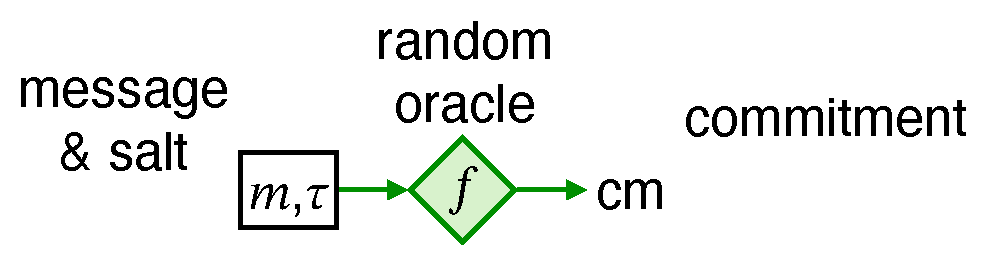
\includegraphics[width=0.5\textwidth]{\FigureFolder/basic-commitment-diagram}
\caption{Diagram of the basic commitment scheme $\CMSymbol$.}
\label{figure:basic-commitment-diagram}
\end{figure}

%%%%%%%%%%%%%%%%%%%%%%%%%%%%%%%%%%%%%%%%%%%%%%%%%%%%%%%%%%%%%%%%%%%%%%%%%%%%%%%
%%%%%%%%%%%%%%%%%%%%%%%%%%%%%%%%%%%%%%%%%%%%%%%%%%%%%%%%%%%%%%%%%%%%%%%%%%%%%%%
%%%%%%%%%%%%%%%%%%%%%%%%%%%%%%%%%%%%%%%%%%%%%%%%%%%%%%%%%%%%%%%%%%%%%%%%%%%%%%%
\section{Binding}
\label{section:basic-commitment-binding}

We prove that $\CMSymbol$ is \emph{binding}: an adversary cannot find two distinct messages that open the same commitment. In more detail, we consider an experiment where the adversary, given access to a random oracle $\ROFunction$, is challenged to output a commitment $\CMCommitment$ and two message-salt pairs $(\CMMessage_{0},\CMSaltString_{0})$ and $(\CMMessage_{1},\CMSaltString_{1})$ such that:
\begin{inparaenum}[(i)]
  \item the messages $\CMMessage_{0}$ and $\CMMessage_{1}$ are distinct (and the salts $\CMSaltString_{0}$ and $\CMSaltString_{1}$ may or may not be distinct); and
  \item $\CMCheck^{\ROFunction}(\CMCommitment,\CMMessage_{0},\CMSaltString_{0})=1$ and $\CMCheck^{\ROFunction}(\CMCommitment,\CMMessage_{1},\CMSaltString_{1})=1$.
\end{inparaenum}
The maximum winning probability of an adversary in this experiment is the \emph{binding error} of $\CMSymbol$.

Breaking the binding property of $\CMSymbol$ is related to finding collisions in the random oracle, because the aforementioned condition of opening the same commitment via two different messages is equivalent to $\ROFunction(\CMMessage_{0},\CMSaltString_{0})=\ROFunction(\CMMessage_{1},\CMSaltString_{1})$ for $\CMMessage_{0} \neq \CMMessage_{1}$.

By the discussion on finding collisions in \Cref{section:collision-resistance}, the binding error is $\Omega(\frac{\ROQueryBound^2}{2^{\ROOutputSize}})$: the collision-finding strategy in the proof of \Cref{claim:collision-lower-bound} can be modified in a straightforward way to find, with probability $\Omega(\frac{\ROQueryBound^2}{2^{\ROOutputSize}})$, $(\CMMessage_{0},\CMSaltString_{0})$ and $(\CMMessage_{1},\CMSaltString_{1})$ such that $\CMMessage_{0} \neq \CMMessage_{1}$ and $\ROFunction(\CMMessage_{0},\CMSaltString_{0})=\ROFunction(\CMMessage_{1},\CMSaltString_{1})$. On the other hand, the lemma below states that any $\ROQueryBound$-query algorithm can break the binding property with probability at most $O(\frac{\ROQueryBound^2}{2^{\ROOutputSize}})$, where the probability is taken over the choice of random oracle. The proof relies on collision resistance of the random oracle, as well as on unpredictability of the random oracle for an edge case in the analysis. Note that the salt size $\CMSaltSize$ of $\CMSymbol$ does \emph{not} play a role in this upper bound, and in particular it can be zero.

\begin{lemma}[$\CMSymbol$ is binding]
\label{lemma:cm-binding}
Let $\CMSymbol \DefineEqual \CMConstructor{\ROOutputSize}{\CMMessageLength}{\CMSaltSize}$. For every query bound $\ROQueryBound \in \Naturals$ and $\ROQueryBound$-query algorithm $\CMAdversary$ (that outputs a commitment $\CMCommitment$, messages $\CMMessage_{0},\CMMessage_{0}$, and salts $\CMSaltString_{0},\CMSaltString_{1}$), if $\ROQueryBound \geq 2$ then
\begin{equation*}
\Pr\left[
\begin{array}{l}
\CMMessage_{0} \neq \CMMessage_{1} \\
\land\;\CMCheck^{\ROFunction}(\CMCommitment,\CMMessage_{0},\CMSaltString_{0})=1 \\
\land\;\CMCheck^{\ROFunction}(\CMCommitment,\CMMessage_{1},\CMSaltString_{1})=1
\end{array}
\GivenExperiment
\StateExperiment{
\ROFunction \gets \RODistribution{\ROOutputSize} \\
(\CMCommitment,\CMMessage_{0},\CMSaltString_{0},\CMMessage_{1},\CMSaltString_{1}) \gets \CMAdversary^{\ROFunction}
}
\right]
\leq
\CMBindingExpression{\ROOutputSize}{\ROQueryBound}
\enspace.
\end{equation*}
\end{lemma}

\begin{proof}
The condition in the probability statement is, by definition of $\CMCheck$, equivalent to
\begin{equation*}
\CMMessage_{0} \neq \CMMessage_{1}
\TextAndInMath
\ROFunction(\CMMessage_{0},\CMSaltString_{0})
=
\ROFunction(\CMMessage_{1},\CMSaltString_{1})
\enspace.
\end{equation*}
In particular, $(\CMMessage_{0},\CMSaltString_{0})$ and $(\CMMessage_{1},\CMSaltString_{1})$ form a collision for $\ROFunction$.

Let $\Event$ be the event that $\CMAdversary$ makes the queries $(\CMMessage_{0},\CMSaltString_{0})$ and $(\CMMessage_{1},\CMSaltString_{1})$ to $\ROFunction$ (i.e., the query-answer trace of $\CMAdversary$ contains $(\CMMessage_{0},\CMSaltString_{0})$ and $(\CMMessage_{1},\CMSaltString_{1})$ as queries). We distinguish between two cases.
\begin{itemize}
  \item \emph{Case 1: $\CMAdversary$ wins the binding game and $\Event$ does not hold.} In this case $\CMAdversary$ outputs $(\CMMessage_{0},\CMSaltString_{0})$ and $(\CMMessage_{1},\CMSaltString_{1})$ that are a collision and either:
\begin{inparaenum}[(i)]
  \item neither pair was queried, or
  \item exactly one pair was queried.
\end{inparaenum}
By the unpredictability property of a random oracle (\Cref{lemma:rom-not-queried-pair}), the probability that either happens is $\ROPExpression{\ROOutputSize}$ because, in either case, $\CMAdversary$ outputs a string that is not part of the query-answer trace $\ROTrace$ and the random oracle $\ROFunction$ maps to a certain output.

  \item \emph{Case 2: $\CMAdversary$ wins the binding game and $\Event$ holds.} In this case the query-answer trace $\ROTrace$ of $\CMAdversary$ contains a collision, because $(\CMMessage_{0},\CMSaltString_{0})$ and $(\CMMessage_{1},\CMSaltString_{1})$ are contained in $\ROTrace$ and satisfy $\ROFunction(\CMMessage_{0},\CMSaltString_{0}) = \ROFunction(\CMMessage_{1},\CMSaltString_{1})$. By \Cref{lemma:rom-cr} the probability that $\ROTrace$ contains a collision is at most $\ROCRExpression{\ROOutputSize}{\ROQueryBound}$.

\end{itemize}
We conclude that
\begin{align*}
&\Pr\left[
\begin{array}{c}
\text{$\CMAdversary$ wins the} \\
\text{binding game}
\end{array}
\right] \\
=&
\Pr\left[
\begin{array}{c}
\text{$\CMAdversary$ wins the} \\
\text{binding game}
\end{array}
\land
\Event
\right]
+
\Pr\left[
\begin{array}{c}
\text{$\CMAdversary$ wins the} \\
\text{binding game}
\end{array}
\land
\Negate{\Event}
\right]
\\ \leq &
\frac{1}{2} \cdot \frac{(\ROQueryBound-1) \cdot \ROQueryBound}{2^{\ROOutputSize}} + \frac{1}{2^{\ROOutputSize}}
\\ = &
\frac{1}{2} \cdot \frac{\ROQueryBound^2 - \ROQueryBound + 2}{2^{\ROOutputSize}}
\enspace.
\end{align*}
Finally, if $\ROQueryBound \geq 2$ then the last expression above is at most $\CMBindingExpression{\ROOutputSize}{\ROQueryBound}$.
\end{proof}

\begin{remark}[statistical binding]
\label{remark:cm-statistical-binding}
The binding property of $\CMSymbol$ in \Cref{lemma:cm-binding} is \emph{computational} because the binding error $\CMBindingExpression{\ROOutputSize}{\ROQueryBound}$ is small only if the adversary makes a bounded number of queries $\ROQueryBound$ to the random oracle. However, if the output size $\ROOutputSize$ of the random oracle is large enough, then $\CMSymbol$ achieves \emph{statistical} binding, namely, a binding property that holds event against adversaries that make an unbounded number of queries to the random oracle (think of $\ROQueryBound=\infty$). The statistical security comes from the simple fact that, if $\ROOutputSize$ is large enough, the commitment scheme $\CMSymbol$ is \emph{injective} with high probability over the choice of random oracle, in which case each commitment has a single preimage (and thus \DoQuote{collisions} do not exist).

To see this, we upper bound the probability that the commitment scheme $\CMSymbol$ is not injective:
\begin{align*}
& \Pr\left[
\begin{array}{l}
\exists\,\CMMessage_{0}, \CMMessage_{1} \in \Bits^{\CMMessageLength}
\text{ with } \CMMessage_{0} \neq \CMMessage_{1} \\
\exists\,\CMSaltString_{0},\CMSaltString_{1} \in \Bits^{\CMSaltSize}
\end{array}
\text{ s.t. }
\CMCommit(\CMMessage_{0},\CMSaltString_{0}) = \CMCommit(\CMMessage_{1},\CMSaltString_{1})
\right]
\\ & \leq
2^{2 \cdot (\CMMessageLength + \CMSaltSize)} \cdot \Pr[
\CMCommit(0^{\CMMessageLength},0^{\CMSaltSize})
=
\CMCommit(1^{\CMMessageLength},0^{\CMSaltSize})]
\\ & =
2^{2 \cdot (\CMMessageLength + \CMSaltSize)} \cdot
\frac{1}{2^{\ROOutputSize}}
\\ & =
\frac{1}{2^{\ROOutputSize - 2 \cdot (\CMMessageLength + \CMSaltSize)}}
\enspace.
\end{align*}
We conclude that the probability that $\CMSymbol$ is injective is at least $1-\frac{1}{2^{\ROOutputSize - 2 \cdot (\CMMessageLength + \CMSaltSize)}}$, which is close to $1$ if $\ROOutputSize \gg 2 \cdot (\CMMessageLength + \CMSaltSize)$. This regime of parameters is, however, not relevant for the setting of succinct arguments (where we need the commitment size $\ROOutputSize$ to be much smaller than the message size $\CMMessageLength$), and so we limit the discussion of statistical binding to this remark.

Note that, conversely, whenever the commitment scheme $\CMSymbol$ is not injective (with respect to messages), an adversary that makes sufficiently many queries to the random oracle can indeed find distinct messages $\CMMessage_{0}$ and $\CMMessage_{1}$ such that $\CMCommit(\CMMessage_{0},\CMSaltString_{0}) = \CMCommit(\CMMessage_{1},\CMSaltString_{1})$ for some salts $\CMSaltString_{0}$ and $\CMSaltString_{1}$, and thereby break the binding property.
\end{remark}

%%%%%%%%%%%%%%%%%%%%%%%%%%%%%%%%%%%%%%%%%%%%%%%%%%%%%%%%%%%%%%%%%%%%%%%%%%%%%%%
%%%%%%%%%%%%%%%%%%%%%%%%%%%%%%%%%%%%%%%%%%%%%%%%%%%%%%%%%%%%%%%%%%%%%%%%%%%%%%%
%%%%%%%%%%%%%%%%%%%%%%%%%%%%%%%%%%%%%%%%%%%%%%%%%%%%%%%%%%%%%%%%%%%%%%%%%%%%%%%
\section{Extractability}
\label{section:basic-commitment-extractability}

We prove that $\CMSymbol$ is \emph{extractable}, which informally means that if an adversary outputs a commitment that it subsequently opens then the adversary \DoQuote{knew} the opening at commitment time. In \Cref{section:basic-commitment-single-extractability} we study this property for one commitment and in \Cref{section:basic-commitment-multi-extractability} we study it for multiple commitments; then in \Cref{section:basic-commitment-extractability-implies-binding} we explain how extractability implies binding.

%%%%%%%%%%%%%%%%%%%%%%%%%%%%%%%%%%%%%%%%%%%%%%%%%%%%%%%%%%%%%%%%%%%%%%%%%%%%%%%
%%%%%%%%%%%%%%%%%%%%%%%%%%%%%%%%%%%%%%%%%%%%%%%%%%%%%%%%%%%%%%%%%%%%%%%%%%%%%%%
\subsection{Extraction for one commitment}
\label{section:basic-commitment-single-extractability}

The extractability property is formalized via an efficient algorithm $\CMExtractor$ called an \emph{extractor}. We consider an experiment of the following form.
\begin{itemize}

  \item In a commitment phase, the adversary, given oracle access to the random oracle, performs a computation and outputs a commitment $\CMCommitment$ and a private state $\ROAdvState$. Let $\ROTrace$ be the query-answer trace of the adversary in this phase.

  \item Then, in an opening phase, the adversary, given oracle access to the random oracle and as input the private state $\ROAdvState$, continues its computation and outputs a message $\CMMessage$ and salt $\CMSaltString$.

\end{itemize}
Extractability states that if the adversary's output message $\CMMessage$ and salt $\CMSaltString$ are a valid opening of the previously-output commitment $\CMCommitment$ then the extractor $\CMExtractor$, given the commitment $\CMCommitment$ and the query-answer trace $\ROTrace$, \emph{also} outputs the same message $\CMMessage$ and salt $\CMSaltString$, up to a small error. In other words, the adversary \DoQuote{knew} the opening $(\CMCommitment,\CMSaltString)$ in the commitment phase because $\CMExtractor$ finds $(\CMCommitment,\CMSaltString)$ by examining only the query-answer trace of the adversary relevant for producing the commitment (without seeing the subsequent query-answer trace in the opening phase).

The lemma below formally states the property and bounds the extraction error, which happens to be the same as the binding error in \Cref{lemma:cm-binding}.

\begin{lemma}[$\CMSymbol$ is extractable]
\label{lemma:cm-extractability}
Let $\CMSymbol \DefineEqual \CMConstructor{\ROOutputSize}{\CMMessageLength}{\CMSaltSize}$. There exists a polynomial-time deterministic algorithm $\CMExtractor$ such that for every query bound $\ROQueryBound \in \Naturals$ and $\ROQueryBound$-query algorithm $\CMAdversary$, if $\ROQueryBound \geq 3$ then
\begin{equation*}
\Pr\left[
\begin{array}{l}
\CMCheck^{\ROFunction}(\CMCommitment,\CMMessage,\CMSaltString)=1 \\
\land\;(\CMMessage',\CMSaltString') \neq (\CMMessage,\CMSaltString)
\end{array}
\GivenExperiment
\StateExperiment{
\ROFunction \gets \RODistribution{\ROOutputSize} \\
\ROOutputAndTrace{\ROFunction}{\CMAdversary}{\ROTrace}{(\CMCommitment,\ROAdvState)} \\
(\CMMessage',\CMSaltString') \gets \CMExtractor(\CMCommitment,\ROTrace) \\
(\CMMessage,\CMSaltString) \gets \CMAdversary^{\ROFunction}(\ROAdvState)
}
\right]
\leq
\CMExtractabilityExpression{\ROOutputSize}{\ROQueryBound}
\enspace.
\end{equation*}
Moreover, $\CMExtractor$ runs in time $O\big(\ROQueryBound \cdot (\CMMessageLength + \CMSaltSize + \ROOutputSize)\big)$.
\end{lemma}

\begin{proof}
We define the extractor $\CMExtractor$ as follows.
\begin{center}
\begin{minipage}{0.9\textwidth}
$\CMExtractor(\CMCommitment,\ROTrace)$:
Search the trace $\ROTrace$ for a query-answer pair of the form $((\CMMessage',\CMSaltString'),\CMCommitment)$, where $\CMMessage' \in \Bits^{\CMMessageLength}$ is a message and $\CMSaltString' \in \Bits^{\CMSaltSize}$ is a salt. If no such pair exists in $\ROTrace$ then abort. If such a pair is found then output $(\CMMessage',\CMSaltString')$.
\end{minipage}
\end{center}
The extractor has the stated time complexity because it scans a query-answer trace consisting of at most $\ROQueryBound$ entries, in order to search for a $(\CMMessageLength + \CMSaltSize + \ROOutputSize)$-bit entry where the answer equals $\CMCommitment$.

We argue that the extractor satisfies the statement.

Fix any $\ROQueryBound_{1},\ROQueryBound_{2} \in \Naturals$ such that $\ROQueryBound_{1} + \ROQueryBound_{2} \leq \ROQueryBound$. Let $\ROTrace'$ be the query-answer trace of the computation $(\CMMessage,\CMSaltString) \gets \CMAdversary^{\ROFunction}(\ROAdvState)$. We prove the upper bound of $\CMExtractabilityExpression{\ROOutputSize}{\ROQueryBound}$ conditioned on the event that $\ROQueryBound_{1} = \Cardinality{\ROTrace}$ and $\ROQueryBound_{2} = \Cardinality{\ROTrace'}$. Then the lemma follows because this upper bound holds for every $\ROQueryBound_{1},\ROQueryBound_{2} \in \Naturals$ such that $\ROQueryBound_{1} + \ROQueryBound_{2} \leq \ROQueryBound$, and every computation of the $\ROQueryBound$-query adversary $\CMAdversary$ implies a setting of $\ROQueryBound_{1},\ROQueryBound_{2}$.

If $\CMCheck^{\ROFunction}(\CMCommitment,\CMMessage,\CMSaltString)=1$ and $\CMExtractor(\CMCommitment,\ROTrace)$ outputs $(\CMMessage',\CMSaltString')$ such that $(\CMMessage',\CMSaltString') \neq (\CMMessage,\CMSaltString)$ then one of the following cases must hold.
\begin{itemize}

  \item There are two or more queries in the query-answer trace $\ROTrace$ whose answer is $\CMCommitment$. By \Cref{lemma:rom-cr} the probability that this happens is at most $\ROCRExpression{\ROOutputSize}{\ROQueryBound_{1}}$.

  \item There exists a query $(\CMMessage_{j},\CMSaltString_{j})$ in $\ROTrace'$ whose answer is $\CMCommitment$ that is not a query in $\ROTrace$. For every query $(\CMMessage_{j},\CMSaltString_{j})$ in $\ROTrace'$, the probability that $\ROFunction(\CMMessage_{j},\CMSaltString_{j}) = \CMCommitment$ is $\ROPExpression{\ROOutputSize}$. Hence by a union bound the probability that there exists such a query is at most $\ROQueryBound_{2} \cdot \ROPExpression{\ROOutputSize}$.

  \item The adversary $\CMAdversary$ outputs $(\CMMessage,\CMSaltString)$ such that $ \ROFunction(\CMMessage,\CMSaltString)=\CMCommitment$ but $((\CMMessage,\CMSaltString),\CMCommitment)$ is not a query-answer pair in $\ROTrace$ or $\ROTrace'$. By \Cref{lemma:rom-not-queried-pair}, the probability that this happens is at most $\ROPExpression{\ROOutputSize}$.

\end{itemize}
We conclude that the extraction error is at most
\begin{align*}
&\ROCRExpression{\ROOutputSize}{\ROQueryBound_{1}}
+ \ROQueryBound_{2} \cdot \ROPExpression{\ROOutputSize}
+ \ROPExpression{\ROOutputSize} \\
&= \frac{1}{2} \cdot \frac{\ROQueryBound_{1}^2-\ROQueryBound_{1}+2\ROQueryBound_{2}+2}{2^{\ROOutputSize}} \\
&\leq \frac{1}{2} \cdot \frac{\ROQueryBound_{1}^2-\ROQueryBound_{1}+2(\ROQueryBound-\ROQueryBound_{1})+2}{2^{\ROOutputSize}} \EquationComment{since $\ROQueryBound_{1}+\ROQueryBound_{2} \leq \ROQueryBound$} \\
&= \frac{1}{2} \cdot \frac{\ROQueryBound_{1}^2-3\ROQueryBound_{1}+2\ROQueryBound+2}{2^{\ROOutputSize}} \\
&\leq \frac{1}{2} \cdot \frac{\max\{2\ROQueryBound+2,\ROQueryBound^2-\ROQueryBound+2\}}{2^{\ROOutputSize}}
\enspace.
\end{align*}
The last inequality is due to the fact that the expression is a convex function in $\ROQueryBound_{1}$ so its maximum on the interval $\ROQueryBound_{1} \in \{0,1,\dots,\ROQueryBound\}$ is achieved at either $\ROQueryBound_{1}=0$ or $\ROQueryBound_{1}=\ROQueryBound$.

Finally, if $\ROQueryBound \geq 3$ then the last expression above is at most $\frac{1}{2} \cdot \frac{\ROQueryBound^2-\ROQueryBound+2}{2^{\ROOutputSize}}$ (in the maximum the first term is at most the second term), which in turn is at most $\CMExtractabilityExpression{\ROOutputSize}{\ROQueryBound}$.
\end{proof}

%%%%%%%%%%%%%%%%%%%%%%%%%%%%%%%%%%%%%%%%%%%%%%%%%%%%%%%%%%%%%%%%%%%%%%%%%%%%%%%
%%%%%%%%%%%%%%%%%%%%%%%%%%%%%%%%%%%%%%%%%%%%%%%%%%%%%%%%%%%%%%%%%%%%%%%%%%%%%%%
\subsection{Extraction for multiple commitments}
\label{section:basic-commitment-multi-extractability}

We discuss how extractability extends to adversaries that output \emph{multiple} commitments. This serves as a warm up to similar properties that we study for Merkle commitments in \Cref{chapter:merkle-commitment}, which we use to analyze constructions of succinct arguments that involve multiple commitments.

We wish to prove that for any commitment that the adversary subsequently opens successfully, the extractor is able to find a corresponding opening while only given the query-answer trace of the adversary up to the point of producing that commitment. (We cannot expect to say anything about commitments that the adversary outputs but does not open successfully.)

We consider an experiment of the following form.
\begin{itemize}

  \item In a commitment phase, the adversary, given oracle access to the random oracle, performs a stateful computation during which it outputs $\CMNumCommitments$ commitments $\CMCommitment_{1},\dots,\CMCommitment_{\CMNumCommitments}$. Let $\ROAdvState_{i}$ be the private state of the adversary when it outputs $\CMCommitment_{i}$, and let $\ROTrace_{i}$ be the query-answer trace of the adversary between outputting the $(i-1)$-th commitment and the $i$-th commitment.

  \item Then, in an opening phase, the adversary, given oracle access to the random oracle and as input the private state $\ROAdvState_{\CMNumCommitments}$, concludes its computation and outputs $\CMNumCommitments$ message-salt pairs $\big((\CMMessage_{i},\CMSaltString_{i})\big)_{i \in [\CMNumCommitments]}$.

\end{itemize}
We wish to prove that, for every $i \in [\CMNumCommitments]$, if the message $\CMMessage_{i}$ and salt $\CMSaltString_{i}$ are a valid opening of the previously-output commitment $\CMCommitment_{i}$ then an extractor $\CMMultiExtractor$, given the commitment $\CMCommitment_{i}$ and the query-answer trace $\ROTrace_{1} \concat \cdots \concat \ROTrace_{i}$ (all the query-answer pairs leading to outputting $\CMCommitment_{i}$), \emph{also} outputs the same message $\CMMessage_{i}$ and salt $\CMSaltString_{i}$, up to a small error.

Intuitively, such a statement should follow directly from \Cref{lemma:cm-extractability} via a union bound: if the adversary outputs $\CMNumCommitments$ commitments and subsequently $\CMNumCommitments$ openings, then the probability that there exists one of the openings that is valid but the extractor did not succeed for the corresponding commitment is at most $\CMNumCommitments$ times the error in \Cref{lemma:cm-extractability}.

Perhaps surprisingly, the multiplicative loss of $\CMNumCommitments$ can be avoided. The dominant error incurred in extraction is linked to a global event rather than an event specific to one or another commitment. Indeed, from the proof of \Cref{lemma:cm-extractability}, extraction for a particular commitment fails if the query-answer trace either contains multiple queries whose answer is the commitment (the adversary found a collision) or does not contain a query whose answer is the commitment (the adversary guessed the answer). The former event is global and leads to the dominant error, while the latter event is specific to a single commitment and hence is incurred once per commitment.

This leads to a lemma with the error bound below. We let $\CMMultiExtractor$ be a \emph{stateful} algorithm; hence $\CMMultiExtractor$ may store information from prior invocations and so it suffices, in its $i$-th invocation, to receive only the commitment and query-answer trace corresponding to the $i$-th output of the adversary. Maintaining state across invocations also enables efficiency improvements.

\begin{lemma}[$\CMSymbol$ is multi-extractable]
\label{lemma:cm-multi-extractability}
Let $\CMSymbol \DefineEqual \CMConstructor{\ROOutputSize}{\CMMessageLength}{\CMSaltSize}$. There exists a polynomial-time deterministic \textbf{stateful} algorithm $\CMMultiExtractor$ such that for every query bound $\ROQueryBound \in \Naturals$, $\ROQueryBound$-query algorithm $\CMAdversary$, and number of commitments $\CMNumCommitments \in \Naturals$, if $\ROQueryBound \geq 2\CMNumCommitments$ then
\begin{align*}
&\Pr\left[
\begin{array}{l}
\exists\,i \in [\CMNumCommitments] \text{ such that:} \\
\CMCheck^{\ROFunction}(\CMCommitment_{i},\CMMessage_{i},\CMSaltString_{i})=1 \\
\land\;(\CMMessage_{i}',\CMSaltString_{i}') \neq (\CMMessage_{i},\CMSaltString_{i})
\end{array}
\GivenExperiment
\StateExperiment{
\ROFunction \gets \RODistribution{\ROOutputSize} \\
\text{For $i=1,\dots,\CMNumCommitments$:} \\
\IndentedBullet\ROInputOutputAndTrace{\ROFunction}{\CMAdversary}{\ROAdvState_{i-1}}{\ROTrace_{i}}{(\CMCommitment_{i},\ROAdvState_{i})} \\
\IndentedBullet(\CMMessage_{i}',\CMSaltString_{i}') \gets \CMMultiExtractor(\CMCommitment_{i},\ROTrace_{i}) \\
\big((\CMMessage_{i},\CMSaltString_{i})\big)_{i \in [\CMNumCommitments]} \gets \CMAdversary^{\ROFunction}(\ROAdvState_{\CMNumCommitments})
}
\right]
\\&\leq
\CMMultiExtractabilityExpression{\ROOutputSize}{\ROQueryBound}{\CMNumCommitments}
\enspace.
\end{align*}
Above we denote by $\ROAdvState_{0}$ the empty string for notational simplicity.

Moreover, $\CMMultiExtractor$ runs in time $O\big( \CMNumCommitments \cdot \ROQueryBound \cdot (\CMMessageLength + \CMSaltSize + \ROOutputSize) \big)$ (across the $\CMNumCommitments$ invocations).
\end{lemma}

We provide an intuitive justification for the error expression above, for simplicity for the case with no salts ($\CMSaltSize = 0$). Consider the following adversary. For the first $\CMNumCommitments-1$ commitments, the adversary performs no queries and simply outputs random commitment strings $(\CMCommitment_{i})_{i \in [\CMNumCommitments-1]}$. Then the adversary performs $\ROQueryBound$ distinct queries, using all of its query budget in the last trace $\ROTrace_{\CMNumCommitments}$. If there exists two distinct queries $\ROQuery_{1}$ and $\ROQuery_{2}$ such that $\ROFunction(\ROQuery_{1}) = \ROFunction(\ROQuery_{2})$, then the adversary outputs $\CMCommitment_{\CMNumCommitments} \DefineEqual \ROFunction(\ROQuery_{1})$ and wins (the adversary can open $\CMCommitment_{\CMNumCommitments}$ in two ways). This explains the first term of the error bound. Otherwise, if there exists a query $\ROQuery$ with a response $\ROAnswer \in \{\CMCommitment_{i}\}_{i \in [\CMNumCommitments-1]}$, then the adversary also wins (if $\ROAnswer = \CMCommitment_{i}$ then the extractor fails on $\CMCommitment_{i}$ because it runs given an empty trace while the adversary can open $\CMCommitment_{i}$). This explains the second term in the error bound, as each query has a probability of $\frac{\CMNumCommitments-1}{2^{\ROOutputSize}}$ to hit a previous commitment.

\begin{proof}
The stateful extractor $\CMMultiExtractor$ is similar to the (stateless) extractor $\CMExtractor$ in the proof of \Cref{lemma:cm-extractability}. The extractor $\CMMultiExtractor$ internally maintains the concatenation of all query-answer traces received so far (after the $i$-th invocation it stores the trace $\ROTrace \DefineEqual \ROTrace_{1} \concat \cdots \concat \ROTrace_{i}$), and uses this trace to search for the message and salt corresponding to the given commitment.
\begin{itemize}

  \item[] $\CMMultiExtractor(\CMCommitment_{i},\ROTrace_{i})$:
  \begin{enumerate}[nolistsep]
    \item Append $\ROTrace_{i}$ to the query-answer trace $\ROTrace$ stored in the internal state.
    \item Run $\CMExtractor$ on input $(\CMCommitment_{i},\ROTrace)$. (Search the trace $\ROTrace$ for a query-answer pair of the form $((\CMMessage'_{i},\CMSaltString'_{i}),\CMCommitment_{i})$, where $\CMMessage'_{i} \in \Bits^{\CMMessageLength}$ is a message and $\CMSaltString'_{i} \in \Bits^{\CMSaltSize}$ is a salt. If no such pair exists in $\ROTrace$ then abort. If such a pair is found then output $(\CMMessage'_{i},\CMSaltString'_{i})$.)
  \end{enumerate}
\end{itemize}
By \Cref{lemma:cm-extractability} each invocation of $\CMExtractor$ runs in time at most $O\big(\ROQueryBound \cdot (\CMMessageLength + \CMSaltSize + \ROOutputSize) \big)$, because the stored query-answer trace contains at most $\ROQueryBound$ entries. The $\CMNumCommitments$ invocations yield the claimed total running time. The time complexity can be improved via a suitable use of dynamic data structures in the internal state (and foregoing $\CMExtractor$ as a subroutine); see \Cref{remark:cm-multi-extractor-efficient-implementation}.

We argue that the extractor satisfies the statement.

Fix any $\ROQueryBound_{1},\ROQueryBound_{2} \in \Naturals$ such that $\ROQueryBound_{1} + \ROQueryBound_{2} \leq \ROQueryBound$. Let $\ROTrace'$ be the query-answer trace of the computation $\big((\CMMessage_{i},\CMSaltString_{i})\big)_{i \in [\CMNumCommitments]} \gets \CMAdversary^{\ROFunction}(\ROAdvState_{\CMNumCommitments})$. We prove the upper bound of $\CMMultiExtractabilityExpression{\ROOutputSize}{\ROQueryBound}{\CMNumCommitments}$ conditioned on the event that $\ROQueryBound_{1} = \Cardinality{\ROTrace_{1} \concat \cdots \concat \ROTrace_{\CMNumCommitments}}$ and $\ROQueryBound_{2} = \Cardinality{\ROTrace'}$. Then the lemma follows because this upper bound holds for every $\ROQueryBound_{1},\ROQueryBound_{2} \in \Naturals$ such that $\ROQueryBound_{1} + \ROQueryBound_{2} \leq \ROQueryBound$, and every computation of the $\ROQueryBound$-query adversary $\CMAdversary$ implies a setting of $\ROQueryBound_{1},\ROQueryBound_{2}$.

If there exists $i \in [\CMNumCommitments]$ such that $\CMCheck^{\ROFunction}(\CMCommitment_{i},\CMMessage_{i},\CMSaltString_{i})=1$ and $\CMMultiExtractor(\CMCommitment_{i},\ROTrace_{i})$ outputs $(\CMMessage_{i}',\CMSaltString_{i}')$ such that $(\CMMessage_{i}',\CMSaltString_{i}') \neq (\CMMessage_{i},\CMSaltString_{i})$ then one of the following cases must hold.
\begin{itemize}

  \item \emph{Collision.} The adversary finds a collision in the trace. That is, there are two or more queries in the query-answer trace $\ROTrace_{1} \concat \cdots \concat \ROTrace_{\CMNumCommitments}$ with the same answer (in particular, whose answer is one of $\{ \CMCommitment_{i} \}_{i \in [\CMNumCommitments]}$). By \Cref{lemma:rom-cr} the probability that this happens is at most $\ROCRExpression{\ROOutputSize}{\ROQueryBound_{1}}$.

  \item \emph{Inversion.} The adversary inverts one of the previously given commitments. That is, there exists $i \in [\CMNumCommitments]$ and a query $(\CMMessage,\CMSaltString)$ in $\ROTrace_{i+1} \concat \cdots \concat \ROTrace_{\CMNumCommitments} \concat \ROTrace'$ whose answer is $\CMCommitment_{i}$ that is not a query in $\ROTrace_{1} \concat \cdots \concat \ROTrace_{i}$. For every query $(\CMMessage,\CMSaltString)$ in $\ROTrace_{i+1} \concat \cdots \concat \ROTrace_{\CMNumCommitments} \concat \ROTrace'$, the probability that $\ROFunction(\CMMessage,\CMSaltString)  = \CMCommitment_{i}$ is at most $\ROPExpression{\ROOutputSize}$. Hence by a union bound over $i \in [\CMNumCommitments]$ and all queries, the probability that there exists such an $i \in [\CMNumCommitments]$ and a query is at most $(\ROQueryBound_{1}+\ROQueryBound_{2}) \cdot \frac{\CMNumCommitments}{2^{\ROOutputSize}}$.

  \item \emph{Pure luck.} The adversary is lucky, and $\CMCheck$ accepts even though no collisions or inversions where found. That is, there exists $i \in [\CMNumCommitments]$ such that the adversary $\CMAdversary$ outputs $(\CMMessage,\CMSaltString)$ with $\ROFunction(\CMMessage,\CMSaltString) = \CMCommitment_{i}$ but $((\CMMessage,\CMSaltString),\CMCommitment_{i})$ is not a query-answer pair in $\ROTrace_{1} \concat \cdots \concat \ROTrace_{\CMNumCommitments} \concat \ROTrace'$. By \Cref{lemma:rom-not-queried-pair}, the probability that this happens is at most $\ROPExpression{\ROOutputSize}$. Taking a union bound over $i \in [\CMNumCommitments]$, the probability there exists such an $i \in [\CMNumCommitments]$ is at most $\CMNumCommitments \cdot \ROPExpression{\ROOutputSize}$.

\end{itemize}
We conclude that the extraction error is at most
\begin{align*}
&\ROCRExpression{\ROOutputSize}{\ROQueryBound_{1}}
+ (\ROQueryBound_{1}+\ROQueryBound_{2}) \cdot \frac{\CMNumCommitments}{2^{\ROOutputSize}}
+ \frac{\CMNumCommitments}{2^{\ROOutputSize}} \\
&=
\frac{1}{2} \cdot \frac{\ROQueryBound_{1}^2-\ROQueryBound_{1}+2\CMNumCommitments}{2^{\ROOutputSize}}
+ (\ROQueryBound_{1}+\ROQueryBound_{2}) \cdot \frac{\CMNumCommitments}{2^{\ROOutputSize}} \\
&\leq
\frac{1}{2} \cdot \frac{\ROQueryBound^2-\ROQueryBound+2\CMNumCommitments}{2^{\ROOutputSize}}
+ \ROQueryBound \cdot \frac{\CMNumCommitments}{2^{\ROOutputSize}}
\enspace.
\end{align*}
Finally, if $\ROQueryBound \geq 2\CMNumCommitments$ then the last expression above is at most $\CMMultiExtractabilityExpression{\ROOutputSize}{\ROQueryBound}{\CMNumCommitments}$ (itself at most $\frac{\ROQueryBound^2}{2^{\ROOutputSize}}$).
\end{proof}

\begin{remark}[time complexity of $\CMMultiExtractor$]
\label{remark:cm-multi-extractor-efficient-implementation}
The running time of $\CMMultiExtractor$ stated in \Cref{lemma:cm-multi-extractability} can be improved, by maintaining a \emph{sorted} trace in order to support fast searching. At the start, $\CMMultiExtractor$ initializes an empty search tree that supports inserts and searches in logarithmic time complexity (e.g., an AVL tree). At the $i$-th invocation of $\CMMultiExtractor$, given input $(\CMCommitment_{i},\ROTrace_{i})$, do the following: insert into the search tree the query-answer pairs of $\ROTrace_{i}$ one by one; then search the search tree for a query-answer pair of the form $((\CMMessage'_{i},\CMSaltString'_{i}),\CMCommitment_{i})$ (and abort if no such pair is found). The running time of this implementation is $O((\ROQueryBound + \CMNumCommitments) \cdot \log \ROQueryBound \cdot (\CMMessageLength + \CMSaltSize + \ROOutputSize))$ (the multiplicative term $(\ROQueryBound + \CMNumCommitments) \cdot \log \ROQueryBound$ replaces $\CMNumCommitments \cdot \ROQueryBound$), as we now explain. Each element in the trace consists of $O(\CMMessageLength + \CMSaltSize + \ROOutputSize)$ bits, and there are at most $\ROQueryBound$ elements. Hence, each insert or search operation takes time $O((\CMMessageLength + \CMSaltSize + \ROOutputSize) \cdot \log \ROQueryBound)$. The total number of insert and search operations is $\ROQueryBound + \CMNumCommitments$ ($\ROQueryBound$ inserts and $\CMNumCommitments$ searches), yielding the claimed time.
\end{remark}

%%%%%%%%%%%%%%%%%%%%%%%%%%%%%%%%%%%%%%%%%%%%%%%%%%%%%%%%%%%%%%%%%%%%%%%%%%%%%%%
%%%%%%%%%%%%%%%%%%%%%%%%%%%%%%%%%%%%%%%%%%%%%%%%%%%%%%%%%%%%%%%%%%%%%%%%%%%%%%%
\subsection{Extractability implies binding}
\label{section:basic-commitment-extractability-implies-binding}

The extractability property in \Cref{lemma:cm-extractability} is a strong security guarantee: any bounded-query adversary that opens a commitment must have \DoQuote{known} the opening at commitment time. In fact, \emph{extractability is stronger than binding}: we show that if $\CMSymbol$ satisfies extractability with error $\CMExtractionError$ then $\CMSymbol$ satisfies binding with error $\CMBindingError \leq 2 \cdot \CMExtractionError$ (a closely related error).\footnote{This implication loses a factor of $2$, and we present it merely for didactic purposes. Indeed, for $\CMSymbol$ we prove almost the same errors in \Cref{lemma:cm-binding} (binding error) and \Cref{lemma:cm-extractability} (extraction error).}

Let $\CMAdversary$ be a $\ROQueryBound$-query algorithm that opens a commitment in two ways with probability $\CMBindingError$:
\begin{equation*}
\CMBindingError
\DefineEqual
\Pr\left[
\begin{array}{l}
  \CMMessage_{0} \neq \CMMessage_{1} \\
  \land\;\CMCheck^{\ROFunction}(\CMCommitment,\CMMessage_{0},\CMSaltString_{0})=1 \\
  \land\;\CMCheck^{\ROFunction}(\CMCommitment,\CMMessage_{1},\CMSaltString_{1})=1
\end{array}
\GivenExperiment
\StateExperiment{
\ROFunction \gets \RODistribution{\ROOutputSize} \\
(\CMCommitment,\CMMessage_{0},\CMSaltString_{0},\CMMessage_{1},\CMSaltString_{1}) \gets \CMAdversary^{\ROFunction}
}
\right]
\enspace.
\end{equation*}

Let $\CMAdversary_{e}$ be the $\ROQueryBound$-query algorithm for the extraction game that is defined as follows.
\begin{itemize}[noitemsep]
  \item $\CMAdversary_{e}^{\ROFunction}$: Run $\CMAdversary^{\ROFunction}$ to get $(\CMCommitment,\CMMessage_{0},\CMSaltString_{0},\CMMessage_{1},\CMSaltString_{1})$, set $\ROAdvState \DefineEqual (\CMMessage_{0},\CMSaltString_{0},\CMMessage_{1},\CMSaltString_{1})$, and output $(\CMCommitment,\ROAdvState)$.
  \item $\CMAdversary_{e}^{\ROFunction}(\ROAdvState)$: Sample a random bit $b$ (by using private randomness or via a fresh additional query to the random oracle) and output the message and salt $(\CMMessage_{b},\CMSaltString_{b})$ stored in $\ROAdvState$.
\end{itemize}
Fix any candidate extractor $\CMExtractor$. Consider an output $(\CMCommitment,\CMMessage_{0},\CMSaltString_{0},\CMMessage_{1},\CMSaltString_{1})$ of $\CMAdversary$ that breaks the binding property (i.e., satisfies the conditions in the probability statement above). If we run $\CMExtractor$ on $\CMCommitment$ (the commitment output by $\CMAdversary_{e}$ in the first step) and $\ROTrace$ (the query-answer trace by $\CMAdversary_{e}$ in the first step) then we obtain an output $(\CMMessage,\CMSaltString)$ that, with probability at least $1/2$, satisfies $(\CMMessage,\CMSaltString) \neq (\CMMessage_{b},\CMSaltString_{b})$. This is because the inputs to the extractor $\CMExtractor$ are independent of the bit $b$ (which is sampled by $\CMAdversary_{e}$ after the inputs to $\CMExtractor$ are determined). Moreover, by the definition of $\CMAdversary_{e}$, we know that $\CMCheck^{\ROFunction}(\CMCommitment,\CMMessage_{b},\CMSaltString_{b})=1$ regardless of the choice of bit $b$. We deduce that
\begin{equation*}
\frac{1}{2} \cdot \CMBindingError \leq
\Pr\left[
\begin{array}{l}
  \CMCheck^{\ROFunction}(\CMCommitment,\CMMessage_{b},\CMSaltString_{b})=1 \\
  \land\;(\CMMessage,\CMSaltString) \neq (\CMMessage_{b},\CMSaltString_{b})
\end{array}
\GivenExperiment
\StateExperiment{
  \ROFunction \gets \RODistribution{\ROOutputSize} \\
  \ROOutputAndTrace{\ROFunction}{\CMAdversary_{e}}{\ROTrace}{(\CMCommitment,\ROAdvState)} \\
  (\CMMessage,\CMSaltString) \gets \CMExtractor(\CMCommitment,\ROTrace) \\
  (\CMMessage_{b},\CMSaltString_{b}) \gets \CMAdversary_{e}^{\ROFunction}(\ROAdvState)
}
\right]
\enspace.
\end{equation*}
We conclude that any extraction error $\CMExtractionError$ that can be proved must satisfy the relation $\frac{1}{2} \cdot \CMBindingError \leq \CMExtractionError$ which gives us the desired bound on the binding error $\CMBindingError$.

%%%%%%%%%%%%%%%%%%%%%%%%%%%%%%%%%%%%%%%%%%%%%%%%%%%%%%%%%%%%%%%%%%%%%%%%%%%%%%%
%%%%%%%%%%%%%%%%%%%%%%%%%%%%%%%%%%%%%%%%%%%%%%%%%%%%%%%%%%%%%%%%%%%%%%%%%%%%%%%
%%%%%%%%%%%%%%%%%%%%%%%%%%%%%%%%%%%%%%%%%%%%%%%%%%%%%%%%%%%%%%%%%%%%%%%%%%%%%%%
\section{Hiding}
\label{section:basic-commitment-hiding}

We prove that $\CMSymbol$ is \emph{hiding}, which informally means that a commitment $\CMCommitment$ computed as $\ROFunction(\CMMessage,\CMSaltString)$ for a random $\CMSaltString \in \Bits^{\CMSaltSize}$ reveals no information about $\CMMessage$, up to a small statistical \DoQuote{leakage} error.

In more detail, we compare the output of an adversary $\CMAdversary^{\ROFunction}(\CMCommitment)$ in two cases:
\begin{itemize}[noitemsep]
  \item $\CMCommitment$ is computed as $\ROFunction(\CMMessage,\CMSaltString)$;
  \item $\CMCommitment$ is output by a probabilistic algorithm $\CMSimulator$ that is only given oracle access to $\ROFunction$ (and in particular does not know the message $\CMMessage$).
\end{itemize}
The hiding property requires that the outputs of the adversary in these two cases are statistically close. Moreover, the adversary may choose the message $\CMMessage$ by querying the random oracle $\ROFunction$.

The statistical distance depends, in general, on several parameters:
\begin{inparaenum}[(a)]
  \item the output size $\ROOutputSize \in \Naturals$ of the random oracle;
  \item the message size $\CMMessageLength \in \Naturals$;
  \item the salt size $\CMSaltSize \in \Naturals$; and
  \item the number of queries $\ROQueryBound$ to the random oracle made by the algorithm trying to distinguish between the two distributions.
\end{inparaenum}
In the lemma below we also consider the case where $\ROQueryBound=\infty$, which corresponds to adversaries that can make an unbounded number of queries to the random oracle (in order to choose the message and also in order to distinguish between the two distributions).

\begin{lemma}[$\CMSymbol$ is hiding]
\label{lemma:cm-hiding}
Let $\CMSymbol \DefineEqual \CMConstructor{\ROOutputSize}{\CMMessageLength}{\CMSaltSize}$. There exists a polynomial-time probabilistic algorithm $\CMSimulator$ such that for every query bound $\ROQueryBound \in \Naturals$ and $\ROQueryBound$-query algorithm $\CMAdversary$, the following two distributions are $\CMHidingError(\ROOutputSize,\CMMessageLength,\CMSaltSize,\ROQueryBound)$-close in statistical distance
\begin{equation*}
\left\{
\CMAdversary^{\ROFunction}(\ROAdvState,\CMCommitment)
\GivenExperiment
\StateExperiment{
\ROFunction \gets \RODistribution{\ROOutputSize} \\
(\CMMessage,\ROAdvState) \gets \CMAdversary^{\ROFunction} \\
(\CMCommitment,\CMSaltString) \gets \CMCommit^{\ROFunction}(\CMMessage)
}
\right\}
\TextAndInMath
\left\{
\CMAdversary^{\ROFunction}(\ROAdvState,\CMCommitment)
\GivenExperiment
\StateExperiment{
\ROFunction \gets \RODistribution{\ROOutputSize} \\
(\CMMessage,\ROAdvState) \gets \CMAdversary^{\ROFunction} \\
\CMCommitment \gets \CMSimulator^{\ROFunction}
}
\right\}
\enspace.
\end{equation*}
Above,
\begin{equation*}
\CMHidingError(\ROOutputSize,\CMMessageLength,\CMSaltSize,\ROQueryBound)
\leq
\begin{cases}
\CMHidingExpressionFinite{\CMSaltSize}{\ROQueryBound}
& \text{ if $\ROQueryBound<\infty$} \\
\CMHidingExpressionInfinite{\CMSaltSize}
& \text{ if $\ROQueryBound=\infty$}
\end{cases}
\enspace.
\end{equation*}
Moreover, $\CMSimulator^{\ROFunction}$ outputs a random string in $\Bits^{\ROOutputSize}$.
\end{lemma}

Of course, the bound for $\ROQueryBound=\infty$ is also a bound for $\ROQueryBound<\infty$. This is useful when $\ROQueryBound$ is large compared to $\CMSaltSize$, in which case the expression $\ROQueryBound \cdot 2^{-\CMSaltSize}$ is not small anymore.

Below we prove the upper bounds for the two cases, providing intuition before each analysis.

\parhead{The case of $\ROQueryBound<\infty$}
There is a straightforward $\ROQueryBound$-query distinguishing strategy:
\begin{itemize}[noitemsep]
  \item In the first phase, $\CMAdversary^{\ROFunction}$ outputs $\CMMessage \DefineEqual 0^{\CMMessageLength}$ (some fixed arbitrary message) and $\ROAdvState \DefineEqual \bot$.
  \item In the second phase, $\CMAdversary^{\ROFunction}(\ROAdvState,\CMCommitment)$ repeatedly samples a random salt $\CMSaltString \in \Bits^{\CMSaltSize}$ and checks if $\CMCommitment=\ROFunction(\CMMessage,\CMSaltString)$; if so then it outputs $1$; else if all $\ROQueryBound$ attempts fail then it outputs a random bit $b$.
\end{itemize}
In one case, if $\CMCommitment=\ROFunction(\CMMessage,\CMSaltString)$ for a random salt $\CMSaltString$ then the probability that the above strategy guesses this salt is $\Omega(\ROQueryBound \cdot 2^{-\CMSaltSize})$. (One can obtain an explicit constant by applying the inclusion-exclusion principle.) In the other case, if $\CMCommitment$ is a random string in $\Bits^{\ROOutputSize}$ (independent of $\ROFunction$) then, except with probability $2^{\CMSaltSize-\ROOutputSize}$, no salt $\CMSaltString$ satisfies $\CMCommitment=\ROFunction(\CMMessage,\CMSaltString)$. Overall, the distinguishing strategy leads to a statistical distance between the two cases that is $\Omega(\ROQueryBound \cdot 2^{-\CMSaltSize} - 2^{\CMSaltSize-\ROOutputSize})$.

Below we prove that this strategy is essentially optimal when $\ROOutputSize$ is sufficiently larger than $\CMSaltSize$ (e.g., $\ROOutputSize \geq 2\CMSaltSize$), in which case the lower bound becomes $\Omega(\ROQueryBound \cdot 2^{-\CMSaltSize})$. This is because \emph{every} $\ROQueryBound$-query algorithm $\CMAdversary$ achieves a statistical distance that is at most $\ROQueryBound \cdot 2^{-\CMSaltSize}$.


\begin{proof}[Proof for $\ROQueryBound<\infty$]
The adversary $\CMAdversary$ performs queries in two phases: the first phase leads to $\CMAdversary$ choosing the message $\CMMessage$; and the second phase is after $\CMAdversary$ receives the commitment $\CMCommitment$. Let $\ROTrace_{1}$ be the query-answer trace of the first phase and $\ROTrace_{2}$ the query-answer trace of the second phase. Define $\ROQueryBound_{1} \DefineEqual \Cardinality{\ROTrace_{1}}$ and $\ROQueryBound_{2} \DefineEqual \Cardinality{\ROTrace_{2}}$. Note that $\ROQueryBound_{1} + \ROQueryBound_{2} \leq \ROQueryBound$. The final output of $\CMAdversary$ is a deterministic function of the query-answer pairs in the traces $\ROTrace_{1}$ and $\ROTrace_{2}$ and the commitment $\CMCommitment$. In one experiment $\CMCommitment$ is computed as $\ROFunction(\CMMessage,\CMSaltString)$ and in the other experiment it is computed as $\CMSimulator^{\ROFunction}$. By \Cref{claim:function-and-statistical-distance}, the statistical distance between the final output of $\CMAdversary$ in the two experiments is at most the statistical distance between the following two random variables:
\begin{align*}
\Big(
\ROTrace_{1},\ROFunction(\CMMessage,\CMSaltString),\ROTrace_{2}\Big)
\;\; \text{and} \;\;
\Big(\ROTrace_{1},\CMSimulator^{\ROFunction},\ROTrace_{2}\Big)
\enspace.
\end{align*}
The simulator $\CMSimulator$ outputs a random string in $\Bits^{\ROOutputSize}$.

Let $\Event$ be the event that $(\CMMessage,\CMSaltString)$ is one of the queries in $\ROTrace_{1}$ or $\ROTrace_{2}$. Conditioned on $\Negate{\Event}$, $\ROFunction(\CMMessage,\CMSaltString)$ is random $\Bits^{\ROOutputSize}$, in which case it is distributed as $\CMSimulator^{\ROFunction}$. Therefore the statistical distance between the two random variables above is at most $\Pr[\Event]$, which we upper bound next.

\begin{claim}
\label{claim:cm-hiding-hit-query}
It holds that
\begin{align*}
\Pr[\Event]
=
\Pr\left[
\CMAdversary^{\ROFunction}(\ROAdvState,\CMCommitment) \text{ queries } (\CMMessage,\CMSaltString)
\GivenExperiment
\StateExperiment{
  \ROFunction \gets \RODistribution{\ROOutputSize} \\
  (\CMMessage,\ROAdvState) \gets \CMAdversary^{\ROFunction} \\
  \CMSaltString \gets \Bits^{\CMSaltSize} \\
  \CMCommitment \gets \ROFunction(\CMCommitment,\CMSaltString)
}
\right]
\leq
\ROOWEntropyExpression{\CMSaltSize}
\enspace.
\end{align*}
\end{claim}

\begin{proof}
First, we consider the trace $\ROTrace_{1}$. The probability that $(\CMMessage,\CMSaltString)$ is a query in $\ROTrace_{1}$ is at most $\frac{\Cardinality{\ROTrace_{1}}}{2^{\CMSaltSize}} \leq \frac{\ROQueryBound_{1}}{2^{\CMSaltSize}}$, because $\CMCommitment$ is the answer to the query $(\CMMessage,\CMSaltString)$ where $\CMMessage$ is the message chosen by the adversary and $\CMSaltString$ is a random salt $\CMSaltString \in \Bits^{\CMSaltSize}$ sampled independently of $\ROTrace_{1}$. Next, we consider the queries in $\ROTrace_{2}$, performed after the adversary has chosen the message $\CMMessage$. Conditioned on the query $(\CMMessage,\CMSaltString)$ not appearing in $\ROTrace_{1}$, the probability that any of the queries in $\ROTrace_{2}$ is $(\CMMessage,\CMSaltString)$ equals the same probability but when sampling $\CMSaltString$ \emph{after} the adversary performs the queries in $\ROTrace_{2}$. Formally, we apply \Cref{lemma:rom-ow-high-entropy} with respect to $\ROFunction'(\CMSaltString) \DefineEqual \ROFunction(\CMMessage,\CMSaltString)$, and deduce that the probability that $(\CMMessage,\CMSaltString)$ is a query in $\ROTrace_{2}$ is at most $\frac{\Cardinality{\ROTrace_{2}}}{2^{\CMSaltSize}} \leq \frac{\ROQueryBound_{2}}{2^{\CMSaltSize}}$. Together, we conclude that
\begin{align*}
\Pr[\Event]
\leq
\frac{\ROQueryBound_{1}}{2^{\CMSaltSize}} + \frac{\ROQueryBound_{2}}{2^{\CMSaltSize}}
= \frac{\ROQueryBound}{2^{\CMSaltSize}}
\enspace.
\end{align*}
\end{proof}
\end{proof}

\parhead{The case of $\ROQueryBound=\infty$}
If the distinguisher may query the random oracle an unbounded number of times then it can use strategies that are quite different from the bounded case. In particular, the distinguisher may query the random oracle $\ROFunction$ at every input, and use the information to attempt to learn $\CMMessage$. For example, for some $\ROFunction$, it is the case that $\Pr_{\CMSaltString}\left[\CMMessage = 1 \ConditionedOn \ROFunction(\CMMessage \concat \CMSaltString) = \CMCommitment\right] \gg \Pr_{\CMSaltString}\left[\CMMessage = 0 \ConditionedOn \ROFunction(\CMMessage \concat \CMSaltString) = \CMCommitment\right]$ for $\CMCommitment = \ROFunction(\CMMessage \concat \CMSaltString)$, in which case $\CMAdversary$ can determine $\CMMessage$ from $\CMCommitment$ with good accuracy. Nevertheless, we expect that most random oracles are \DoQuote{well-behaved}: for every image $\CMCommitment \in \Bits^{\ROOutputSize}$ and any two messages $\CMMessage,\CMMessage'$ the number of pre-images of the form $(\CMMessage,\CMSaltString)$ is roughly the same as the number of pre-images of the form $(\CMMessage',\CMSaltString)$. In such a case, it remains (statistically) hard to distinguish if the message is $\CMMessage$ or $\CMMessage'$ (or even $\CMCommitment$ is simply random).

Informally, the error is a sum of two terms: $2^{-2\ROOutputSize \CMMessageLength \CMSaltSize} +
2 \sqrt{\ROOutputSize \CMMessageLength \CMSaltSize} \cdot 2^{-\frac{\CMSaltSize - \ROOutputSize}{2}} = O(\sqrt{\ROOutputSize \CMMessageLength \CMSaltSize} \cdot 2^{-\frac{\CMSaltSize - \ROOutputSize}{2}})$. The first term comes from the probability that a random oracle is not well-behaved. The second term (which is the dominant one) is the statistical distance of a random variable of the form $\ROFunction(\CMMessage \concat \CMSaltString)$ from a random string in $\Bits^{\ROOutputSize}$, for a fixed well-behaved $\ROFunction$ and over a random choice of $\CMSaltString$. In \Cref{claim:cm-tightness-of-unbounded-case} further below we prove that the bound is essentially tight.

\begin{proof}[Proof for $\ROQueryBound=\infty$]
The adversary is unbounded, and so its final output is a deterministic function of the random oracle $\ROFunction$ (in its entirety) and the commitment $\CMCommitment$. In one experiment $\CMCommitment$ is computed as $\ROFunction(\CMMessage,\CMSaltString)$ and in the other experiment it is computed as $\CMSimulator^{\ROFunction}$. By \Cref{claim:function-and-statistical-distance}, the statistical distance between the adversary's final output in the two experiments is at most the statistical distance between the following two random variables:
\begin{align*}
\Big(
\ROFunction,
\ROFunction(\CMMessage,\CMSaltString)
\Big)
\;\; \text{and} \;\;
\Big(
\ROFunction,
\CMSimulator^{\ROFunction}
\Big)
\enspace.
\end{align*}
The simulator $\CMSimulator$ outputs a random string in $\Bits^{\ROOutputSize}$.

For every $\CMMessage \in \Bits^{\CMMessageLength}$, $\CMCommitment \in \Bits^{\ROOutputSize}$, and $\CMSaltString \in \Bits^{\CMSaltSize}$, define $\RandomVariableZ_{\CMMessage,\CMCommitment,\CMSaltString}$ to be the indicator random variable (over the choice of $\ROFunction$) that denotes the event that $\ROFunction(\CMMessage,\CMSaltString) = \CMCommitment$. Note that $(\RandomVariableZ_{\CMMessage,\CMCommitment,\CMSaltString})_{\CMSaltString \in \Bits^{\CMSaltSize}}$ are independent random variables, and that $\Pr[\RandomVariableZ_{\CMMessage,\CMCommitment,\CMSaltString}=1]=2^{-\ROOutputSize}$ for every $\CMSaltString \in \Bits^{\CMSaltSize}$.

For every $\CMMessage \in \Bits^{\CMMessageLength}$ and $\CMCommitment \in \Bits^{\ROOutputSize}$, define $\RandomVariableZ_{\CMMessage,\CMCommitment}$ to be the random variable (over the choice of $\ROFunction$) that counts the number of salts that map the message $\CMMessage$ to the commitment $\CMCommitment$:
\begin{equation*}
\RandomVariableZ_{\CMMessage,\CMCommitment}
\DefineEqual
\sum_{\CMSaltString \in \Bits^{\CMSaltSize}} \RandomVariableZ_{\CMMessage,\CMCommitment,\CMSaltString}
\enspace.
\end{equation*}
Note that $\Expectation[\RandomVariableZ_{\CMMessage,\CMCommitment}] = \sum_{\CMSaltString \in \Bits^{\CMSaltSize}} \Expectation[\RandomVariableZ_{\CMMessage,\CMCommitment,\CMSaltString}] = 2^{\CMSaltSize-\ROOutputSize}$. By a Chernoff bound (\Cref{lemma:chernoff-bound}),
\begin{align*}
\Pr_{\ROFunction}\Big[
\AbsValue{
\RandomVariableZ_{\CMMessage,\CMCommitment}
-
\Expectation[\RandomVariableZ_{\CMMessage,\CMCommitment}]
}
\geq
\delta \cdot \Expectation[\RandomVariableZ_{\CMMessage,\CMCommitment}]
\Big]
\leq 2e^{-\frac{\Expectation[\RandomVariableZ_{\CMMessage,\CMCommitment}] \delta^2}{3}}
\enspace.
\end{align*}
Setting $\delta \DefineEqual 4\sqrt{\frac{\ROOutputSize \CMMessageLength \CMSaltSize}{\Expectation[\RandomVariableZ_{\CMMessage,\CMCommitment}]}} = 4\sqrt{\ROOutputSize \CMMessageLength \CMSaltSize} \cdot 2^{-\frac{\CMSaltSize-\ROOutputSize}{2}}$, we get
\begin{align*}
\Pr_{\ROFunction}\left[
\AbsValue{
\RandomVariableZ_{\CMMessage,\CMCommitment}
-
2^{\CMSaltSize-\ROOutputSize}
}
\geq
4\sqrt{\ROOutputSize \CMMessageLength \CMSaltSize} \cdot 2^{\frac{\CMSaltSize-\ROOutputSize}{2}}
\right]
\leq 2e^{-\frac{16\ROOutputSize \CMMessageLength \CMSaltSize}{3}}
\leq e^{-4\ROOutputSize \CMMessageLength \CMSaltSize}
\enspace.
\end{align*}
Taking a union bound over all $\CMCommitment \in \Bits^{\ROOutputSize}$, and dividing by $2^{\CMSaltSize}$ we deduce that
\begin{align}
\label{eq:hiding-good-event}
\Pr_{\ROFunction}\left[
\exists\,\CMCommitment \in \Bits^{\ROOutputSize}
:
\AbsValue{
\frac{\RandomVariableZ_{\CMMessage,\CMCommitment}}{2^{\CMSaltSize}}
-
\frac{1}{2^{\ROOutputSize}}
}
\geq 4\sqrt{\ROOutputSize \CMMessageLength \CMSaltSize} \cdot 2^{-\frac{\CMSaltSize +  \ROOutputSize}{2}}
\right]
\leq 2^{\ROOutputSize} \cdot e^{-4\ROOutputSize \CMMessageLength \CMSaltSize}
\enspace.
\end{align}

Let $U_{\ROOutputSize}$ be the uniform distribution over $\Bits^{\ROOutputSize}$; also, for a given $\ROFunction$, let $D_{\CMMessage}(\ROFunction)$ be the distribution $\ROFunction(\CMMessage,\CMSaltString)$ for a uniform random salt $\CMSaltString \in \Bits^{\CMSaltSize}$. For every $\ROFunction$ such that the event in \Cref{eq:hiding-good-event} does not hold (namely, for every $\CMCommitment \in \Bits^{\ROOutputSize}$ it holds that $\AbsValue{\frac{\RandomVariableZ_{\CMMessage,\CMCommitment}}{2^{\CMSaltSize}} - \frac{1}{2^{\ROOutputSize}}} < 4\sqrt{\ROOutputSize \CMMessageLength \CMSaltSize} \cdot 2^{-\frac{\CMSaltSize +  \ROOutputSize}{2}}$), we have that
\begin{align*}
& \Delta(D_{\CMMessage}(\ROFunction),U_{\ROOutputSize}) \\
& = \frac{1}{2} \cdot \sum_{\CMCommitment \in \Bits^{\ROOutputSize}} \AbsValue{\frac{\RandomVariableZ_{\CMMessage,\CMCommitment}(\ROFunction)}{2^{\CMSaltSize}} - \frac{1}{2^{\ROOutputSize}}} \\
& < \frac{1}{2} \cdot \sum_{\CMCommitment \in \Bits^{\ROOutputSize}} 4\sqrt{\ROOutputSize \CMMessageLength \CMSaltSize} \cdot 2^{-\frac{\CMSaltSize +  \ROOutputSize}{2}} \\
& = 2 \cdot 2^{\ROOutputSize} \cdot \sqrt{\ROOutputSize \CMMessageLength \CMSaltSize} \cdot 2^{-\frac{\CMSaltSize +  \ROOutputSize}{2}} \\
& = 2 \sqrt{\ROOutputSize \CMMessageLength \CMSaltSize} \cdot 2^{-\frac{\CMSaltSize - \ROOutputSize}{2}}
\enspace.
\end{align*}
Taking a union bound over all $\CMMessage \in \Bits^{\CMMessageLength}$, we deduce that
\begin{align*}
\Pr_{\ROFunction}
\left[\exists\,\CMMessage \in \Bits^{\CMMessageLength} : \StatisticalDistance{D_{\CMMessage}(\ROFunction)}{U_{\ROOutputSize}} \geq 2 \sqrt{\ROOutputSize \CMMessageLength \CMSaltSize} \cdot 2^{-\frac{\CMSaltSize - \ROOutputSize}{2}}
\right]
\leq 2^{\CMMessageLength} \cdot 2^{\ROOutputSize} \cdot e^{-4\ROOutputSize \CMMessageLength \CMSaltSize}
\leq 2^{-2\ROOutputSize \CMMessageLength \CMSaltSize}
\enspace.
\end{align*}
Using \Cref{claim:statistical-distance-for-derived-variables} we conclude that the statistical distance is
\begin{equation*}
\StatisticalDistance{(\ROFunction,D_{\CMMessage}(\ROFunction))}{(\ROFunction,U_{\ROOutputSize})}
\leq
2^{-2\ROOutputSize \CMMessageLength \CMSaltSize} +
2 \sqrt{\ROOutputSize \CMMessageLength \CMSaltSize} \cdot 2^{-\frac{\CMSaltSize - \ROOutputSize}{2}}
\leq
3 \sqrt{\ROOutputSize \CMMessageLength \CMSaltSize} \cdot 2^{-\frac{\CMSaltSize - \ROOutputSize}{2}}
\enspace.
\end{equation*}
\end{proof}

\begin{claim}
\label{claim:cm-tightness-of-unbounded-case}
Let $\CMSymbol \DefineEqual \CMConstructor{\ROOutputSize}{\CMMessageLength}{\CMSaltSize}$. For every message $\CMMessage \in \Bits^{\CMMessageLength}$ there exists an unbounded adversary $\CMAdversary$ for which the following two distributions are $\Omega(2^{-\frac{\CMSaltSize-\ROOutputSize}{2}})$-far in statistical distance:
\begin{equation*}
\left\{
\CMAdversary^{\ROFunction}(\CMCommitment)
\GivenExperiment
\StateExperiment{
  \ROFunction \gets \RODistribution{\ROOutputSize} \\
  (\CMCommitment,\CMSaltString) \gets \CMCommit^{\ROFunction}(\CMMessage)
}
\right\}
\TextAndInMath
\left\{
\CMAdversary^{\ROFunction}(\CMCommitment)
\GivenExperiment
\StateExperiment{
  \ROFunction \gets \RODistribution{\ROOutputSize} \\
  \CMCommitment \gets \CMSimulator^{\ROFunction}
}
\right\}
\enspace.
\end{equation*}
\end{claim}

\begin{proof}
The adversary $\CMAdversary$ performs the following $2^{\CMSaltSize}$-query attack: compute $\Pr_{\CMSaltString}[\ROFunction(\CMMessage,\CMSaltString) = \CMCommitment]$ and output $1$ if and only if this probability is at least $\alpha \DefineEqual 2^{-\ROOutputSize} + \frac{1}{4} \cdot 2^{\frac{-\CMSaltSize - \ROOutputSize-1}{2}}$.

Fix a random oracle $\ROFunction$. For every $\ROAnswer \in \Bits^{\ROOutputSize}$, define $S_{\ROFunction,\ROAnswer} \DefineEqual \{ \CMSaltString \in \Bits^{\CMSaltSize} : \ROFunction(\CMMessage,\CMSaltString) = \ROAnswer \}$. Define $\RandomVariableX_{\ROFunction,\ROAnswer}$ to be $1$ if $\Pr_{\CMSaltString}[\CMSaltString \in S_{\ROFunction,\ROAnswer}] \geq \alpha$, and $0$ otherwise. Define $\RandomVariableX_{\ROFunction} \DefineEqual \sum_{\ROAnswer \in \Bits^{\ROOutputSize}}\RandomVariableX_{\ROFunction,\ROAnswer}$.

For every $\ROFunction \in \RODistribution{\ROOutputSize}$, the probability that $\CMAdversary$ outputs $1$ equals the probability that the random salt $\CMSaltString$ is such that $\RandomVariableX_{\ROFunction,\ROFunction(\CMMessage,\CMSaltString)}=1$. Hence
\begin{align*}
& \Pr\left[
\CMAdversary^{\ROFunction}(\CMCommitment) = 1
\GivenExperiment
\StateExperiment{
  (\CMCommitment,\CMSaltString) \gets \CMCommit^{\ROFunction}(\CMMessage)
}
\right] \\
&=
\Pr\left[
\CMAdversary^{\ROFunction}(\CMCommitment) = 1
\GivenExperiment
\StateExperiment{
  \CMSaltString \gets \Bits^{\CMSaltSize} \\
  \CMCommitment \gets \ROFunction(\CMMessage,\CMSaltString)
}
\right]
\\ & =
\sum_{\ROAnswer \in \Bits^{\ROOutputSize}}\Pr_{\CMSaltString}[\CMSaltString \in S_{\ROFunction,\ROAnswer}] \cdot \RandomVariableX_{\ROFunction,\ROAnswer} \\
&\geq
\sum_{\ROAnswer \in \Bits^{\ROOutputSize}} \alpha \cdot \RandomVariableX_{\ROFunction,\ROAnswer}
=
\alpha \cdot \RandomVariableX_{\ROFunction}
\enspace.
\end{align*}
Averaging over all $\ROFunction$ we get that
\begin{align*}
&\Pr\left[
\CMAdversary^{\ROFunction}(\CMCommitment) = 1
\GivenExperiment
\StateExperiment{
  \ROFunction \gets \RODistribution{\ROOutputSize} \\
  (\CMCommitment,\CMSaltString) \gets \CMCommit^{\ROFunction}(\CMMessage)
}
\right]
\\&=
\Pr\left[
\CMAdversary^{\ROFunction}(\CMCommitment) = 1
\GivenExperiment
\StateExperiment{
  \ROFunction \gets \RODistribution{\ROOutputSize} \\
  \CMSaltString \gets \Bits^{\CMSaltSize} \\
  \CMCommitment \gets \ROFunction(\CMMessage,\CMSaltString)
}
\right]
\geq
\alpha \cdot \Expectation_{\ROFunction}[\RandomVariableX_{\ROFunction}]
\enspace.
\end{align*}
On the other hand,
\begin{align*}
&\Pr\left[
\CMAdversary^{\ROFunction}(\CMCommitment) = 1
\GivenExperiment
\StateExperiment{
  \ROFunction \gets \RODistribution{\ROOutputSize} \\
  \CMCommitment \gets \CMSimulator^{\ROFunction}
}
\right]
\\&= \Pr\left[
\CMAdversary^{\ROFunction}(\CMCommitment) = 1
\GivenExperiment
\StateExperiment{
  \ROFunction \gets \RODistribution{\ROOutputSize} \\
  \CMCommitment \gets \Bits^{\ROOutputSize}
}
\right]
= 2^{-\ROOutputSize} \cdot \Expectation_{\ROFunction}[\RandomVariableX_{\ROFunction}]
\enspace.
\end{align*}
Thus, the statistical distance $\delta$ is at least
\begin{equation*}
\delta
\geq \alpha \cdot \Expectation_{\ROFunction}[\RandomVariableX_{\ROFunction}] - 2^{-\ROOutputSize} \cdot \Expectation_{\ROFunction}[\RandomVariableX_{\ROFunction}]
= \Expectation_{\ROFunction}[\RandomVariableX_{\ROFunction}] \cdot (\alpha - 2^{-\ROOutputSize})
= \Expectation_{\ROFunction}[\RandomVariableX_{\ROFunction}] \cdot \frac{1}{4} \cdot 2^{\frac{-\CMSaltSize - \ROOutputSize-1}{2}}
\enspace.
\end{equation*}
We lower bound $\Expectation_{\ROFunction}[\RandomVariableX_{\ROFunction}]$ in the following claim.

\begin{claim}
$\Expectation_{\ROFunction}[\RandomVariableX_{\ROFunction}] = \Omega(2^{\ROOutputSize})$
\end{claim}

\begin{proof}
We lower bound $\Expectation_{\ROFunction}[\RandomVariableX_{\ROFunction,\ROAnswer}]$ for every $\ROAnswer \in \Bits^{\ROOutputSize}$. The expectation  $\Expectation_{\ROFunction}[\RandomVariableX_{\ROFunction,\ROAnswer}]$ equals the probability that a binomial distribution with $2^{\CMSaltSize}$ experiments and success probability $2^{-\ROOutputSize}$ is at least $2^{\CMSaltSize} \cdot \alpha$. Denoting the binomial probability with $\mathsf{Bin}$, we have that $\Expectation_{\ROFunction}[\RandomVariableX_{\ROFunction,\ROAnswer}] = \Pr[\mathsf{Bin}(2^{\CMSaltSize},2^{-\ROOutputSize}) \geq 2^{\CMSaltSize} \cdot \alpha]$. The binomial distribution can be approximated (up to constant factor) by a normal distribution (denoted by $\mathsf{N}$) as follows: for any $x$, $\Pr[\mathsf{Bin}(n,p) \geq x]  = \Omega(\Pr[\mathsf{N}(np,np(1-p)) \geq x])$. Thus, there is a constant $c > 0$ such that
\begin{align*}
\Expectation_{\ROFunction}[\RandomVariableX_{\ROFunction,\ROAnswer}]
& = \Pr[\mathsf{Bin}(2^{\CMSaltSize},2^{-\ROOutputSize}) \geq 2^{\CMSaltSize} \cdot \alpha]
\\ & \geq
c \cdot \Pr[\mathsf{N}(2^{\CMSaltSize-\ROOutputSize},2^{\CMSaltSize-\ROOutputSize}(1-2^{-\ROOutputSize})) \geq 2^{\CMSaltSize} \cdot \alpha]
\\ & \geq
c \cdot \Pr[\mathsf{N}(2^{\CMSaltSize-\ROOutputSize}, 2^{\CMSaltSize-\ROOutputSize-1}) \geq 2^{\CMSaltSize} \cdot \alpha]
\\ & =
c \cdot \Pr[\mathsf{N}(0, 2^{\CMSaltSize-\ROOutputSize-1}) \geq 2^{\CMSaltSize} \cdot \alpha - 2^{\CMSaltSize-\ROOutputSize}]
\\ & =
c \cdot \Pr\left[\mathsf{N}(0,1) \geq \frac{\alpha - 2^{-\ROOutputSize}}{2^{\frac{-\CMSaltSize-\ROOutputSize-1}{2}}}\right]
\EquationComment{recall that $b \cdot \mathsf{N}(0,\sigma^2) =  \mathsf{N}(0,b^2 \cdot \sigma^2)$.}
\\ & =
c \cdot \Pr\left[\mathsf{N}(0,1) \geq \frac{1}{4}\right]
= \Omega\left(1\right)
\enspace.
\end{align*}
Then, by linearity of expectation, we get that $\Expectation_{\ROFunction}[\RandomVariableX_{\ROFunction}] \geq \Omega(2^{\ROOutputSize})$.
\end{proof}
Plugging this in the lower bound for $\delta$ we get that
\begin{align*}
\delta \geq
\Expectation_{\ROFunction}[\RandomVariableX_{\ROFunction}] \cdot \frac{1}{4} \cdot 2^{\frac{-\CMSaltSize - \ROOutputSize-1}{2}}
 =
\Omega\left(2^{\ROOutputSize} \cdot \frac{1}{4} \cdot 2^{\frac{-\CMSaltSize - \ROOutputSize-1}{2}}\right)
 =
\Omega \left(2^{-\frac{\CMSaltSize-\ROOutputSize}{2}} \right)
\enspace.
\end{align*}
\end{proof}




%%%%%%%%%%%%%%%%%%%%%%%%%%%%%%%%%%%%%%%%%%%%%%%%%%%%%%%%%%%%%%%%%%%%%%%%%%%%%%%
%%%%%%%%%%%%%%%%%%%%%%%%%%%%%%%%%%%%%%%%%%%%%%%%%%%%%%%%%%%%%%%%%%%%%%%%%%%%%%%
%%%%%%%%%%%%%%%%%%%%%%%%%%%%%%%%%%%%%%%%%%%%%%%%%%%%%%%%%%%%%%%%%%%%%%%%%%%%%%%
%%%%%%%%%%%%%%%%%%%%%%%%%%%%%%%%%%%%%%%%%%%%%%%%%%%%%%%%%%%%%%%%%%%%%%%%%%%%%%%
\chapter{Merkle commitment scheme}
\label{chapter:merkle-commitment}

We describe the \emph{Merkle commitment scheme}, a commitment scheme in the ROM that produces succinct commitments to long lists of values and enables to cheaply open particular subsets of vales in the list. This useful \DoQuote{succinct opening} property is used to construct succinct arguments in the ROM.\footnote{More generally, succinct commitments with succinct opening are known as \emph{vector commitments} in the cryptography literature, and constructions are known from various cryptographic assumptions. They are used to construct succinct arguments in various settings also beyond the (pure) ROM.} The commitment scheme is so called because it relies on Merkle trees \cite{Merkle89-tree}, a powerful and versatile data structure based on hash functions. A Merkle commitment scheme uses the basic commitment scheme $\CMSymbol$ as a building block, so throughout this chapter we assume familiarity with the material in \Cref{chapter:basic-commitment}.

\parhead{Organization}
In \Cref{section:merkle-commitment-definition} we describe the construction of a Merkle commitment scheme, and discuss its efficiency properties. Then in \Cref{section:merkle-commitment-completeness} we discuss its \emph{completeness property}, that is, how an honest use of the commitment scheme always leads to successful validity checks. After that we discuss security properties. In \Cref{section:merkle-commitment-collision-lemma} we establish a technical property that we use in several analyses. Finally, we discuss the main security properties of a Merkle commitment scheme:
\begin{itemize}[noitemsep]
  \item in \Cref{section:merkle-commitment-binding} we prove that $\MTSymbol$ is \emph{binding};
  \item in \Cref{section:merkle-commitment-extractability} we prove that $\MTSymbol$ is \emph{extractable};
  \item in \Cref{section:merkle-commitment-hiding} we prove that $\MTSymbol$ is \emph{hiding}.
\end{itemize}

%%%%%%%%%%%%%%%%%%%%%%%%%%%%%%%%%%%%%%%%%%%%%%%%%%%%%%%%%%%%%%%%%%%%%%%%%%%%%%%
%%%%%%%%%%%%%%%%%%%%%%%%%%%%%%%%%%%%%%%%%%%%%%%%%%%%%%%%%%%%%%%%%%%%%%%%%%%%%%%
%%%%%%%%%%%%%%%%%%%%%%%%%%%%%%%%%%%%%%%%%%%%%%%%%%%%%%%%%%%%%%%%%%%%%%%%%%%%%%%
\section{Definition}
\label{section:merkle-commitment-definition}

A \emph{Merkle commitment scheme} is a tuple of three algorithms:
\begin{equation*}
\MTSymbol = (\MTCommit,\MTOpen,\MTCheck)
\enspace.
\end{equation*}
The scheme has several parameters: an output size $\ROOutputSize \in \Naturals$ of the random oracle, a message alphabet $\MTAlphabet$, a message length $\MTMessageLength$, and a salt size $\MTSaltSize \in \Naturals$. We use the notation $\MTConstructor{\ROOutputSize}{\MTAlphabet}{\MTMessageLength}{\MTSaltSize}$ when we wish to make these parameters explicit.

The algorithms receive query access to a random oracle $\ROFunction \in \RODistribution{\ROOutputSize}$ and have the following syntax.
\begin{itemize}
  \item \emph{Commit.}
  The algorithm $\MTCommit$ receives as input a message vector $\MTMessageVector \in \MTAlphabet^{\MTMessageLength}$, and computes a Merkle commitment $\MTCommitment \in \Bits^{\ROOutputSize}$ and corresponding opening trapdoor $\MTTrapdoor \in \Bits^{O((\MTSaltSize + \ROOutputSize) \cdot \MTMessageLength)}$. This algorithm is probabilistic if privacy is desired (otherwise it is deterministic).
  \item \emph{Open.}
  The algorithm $\MTOpen$ receives as input opening trapdoor $\MTTrapdoor$ and a subset $\MTMessageIndexSet \subseteq [\MTMessageLength]$, and computes an opening proof $\MTProof$ that authenticates the values at the locations in $\MTMessageIndexSet$.
  \item \emph{Check.}
  The algorithm $\MTCheck$ receives as input a Merkle commitment $\MTCommitment$, subset $\MTMessageIndexSet \subseteq [\MTMessageLength]$, claimed values $\MTMessageSubVector \in \MTAlphabet^{\MTMessageIndexSet}$, and opening proof $\MTProof$, and computes a bit indicating whether the opening proof $\MTProof$ authenticates $\MTMessageSubVector$ as values for the locations in $\MTMessageIndexSet$ with respect to $\MTCommitment$.
\end{itemize}
Henceforth we assume that $\MTMessageLength$ is a power of $2$; see \Cref{remark:mt-any-message-length} for a discussion of how to remove this assumption.

\parhead{Binary tree}
We introduce notation for a (perfect) binary tree on $\MTMessageLength$ leaves,\footnote{A binary tree is \emph{perfect} if all internal vertices have two children and all leaf vertices belong to the same layer.} which then we use to describe the algorithms of the Merkle commitment scheme. Those algorithms can be viewed as labeling (or checking the labels of) vertices of this (perfect) binary tree.

\begin{definition}
\label{definition:mt-graph}
For $\MTMessageLength \in \Naturals$, $\MTGraph_{\MTMessageLength} = (\MTVertexSet_{\MTMessageLength},\MTEdgeSet_{\MTMessageLength})$ is the (perfect) \defemph{binary tree graph} of depth
\begin{equation}
\label{equation:mt-depth-definition}
\MTDepth \DefineEqual \log_{2} \MTMessageLength
\end{equation}
where the vertex set $\MTVertexSet_{\MTMessageLength}$ and edge set $\MTEdgeSet_{\MTMessageLength}$ are defined as follows:
\begin{align*}
\MTVertexSet_{\MTMessageLength} &\DefineEqual \left\{ (\MTLayer,\MTMessageIndex) : \MTLayer \in \{0,1,\dots,\MTDepth\} , \MTMessageIndex \in [2^{\MTLayer}] \right\} \enspace, \\
\MTEdgeSet_{\MTMessageLength} &\DefineEqual \left\{ \big((\MTLayer-1,\MTMessageIndex),(\MTLayer,2\MTMessageIndex-b)\big) : \MTLayer \in \{1,\dots,\MTDepth\} , \MTMessageIndex \in [2^{\MTLayer-1}] , b \in \{1,0\} \right\} \enspace.
\end{align*}
\end{definition}

We use the depth $\MTDepth$ throughout this chapter without explicitly re-defining it as in \Cref{equation:mt-depth-definition}.

\begin{definition}
\label{definition:mt-paths}
We make the following notational definitions:
\begin{itemize}[nolistsep]
  \item The \defemph{root vertex} of $\MTGraph_{\MTMessageLength}$ is the vertex $(0,1)$.
  \item The \defemph{leaf vertices} of $\MTGraph_{\MTMessageLength}$ are the vertices $\{(\MTDepth,\MTMessageIndex)\}_{\MTMessageIndex \in [\MTMessageLength]}$.
  \item A vertex $(\MTLayer,\MTMessageIndex)$ is \defemph{odd} if $\MTMessageIndex$ is odd and it is \defemph{even} if $\MTMessageIndex$ is even.
  \item The \defemph{sibling} of a non-root vertex $(\MTLayer,\MTMessageIndex)$ (i.e., with $\MTLayer > 0$) is $(\MTLayer,\MTMessageIndex+1)$ if $(\MTLayer,\MTMessageIndex)$ is odd and is $(\MTLayer,\MTMessageIndex-1)$ if $(\MTLayer,\MTMessageIndex)$ is even.
  \item The \defemph{path} from the $\MTMessageIndex$-th leaf vertex $(\MTDepth,\MTMessageIndex)$ to the root vertex is denoted by $\MTPath(\MTMessageIndex)$; the vertex in $\MTPath(\MTMessageIndex)$ that is in layer $\MTLayer$ is denoted $\MTPathIndex{\MTMessageIndex}{\MTLayer} \in \{\MTLayer\} \times [2^{\MTLayer}]$.
  \item The \defemph{copath} from the $\MTMessageIndex$-th leaf vertex $(\MTDepth,\MTMessageIndex)$ to the root vertex is denoted by $\MTCoPath(\MTMessageIndex)$, and is the list of siblings of each vertex in $\MTPath(\MTMessageIndex)$, except the root vertex (which has no siblings); the vertex in $\MTCoPath(\MTMessageIndex)$ that is in layer $\MTLayer$ is denoted $\MTPathCoIndex{\MTMessageIndex}{\MTLayer} \in \{\MTLayer\} \times [2^{\MTLayer}]$ (and is the sibling of $\MTPathIndex{\MTMessageIndex}{\MTLayer}$).
  \item For $\MTMessageIndexSet \subseteq [\MTMessageLength]$, $\MTPath(\MTMessageIndexSet) \DefineEqual \idxcup{\MTMessageIndex \in \MTMessageIndexSet} \MTPath(\MTMessageIndex)$ and $\MTCoPath(\MTMessageIndexSet) \DefineEqual \idxcup{\MTMessageIndex \in \MTMessageIndexSet} \MTCoPath(\MTMessageIndex)$ (viewing lists as sets).
\end{itemize}
\end{definition}

Using this notation we can write:
\begin{equation*}
\MTPath(\MTMessageIndex)
=
\Big(
\MTPathIndex{\MTMessageIndex}{\MTLayer}
\Big)_{\MTLayer \in \{0,1,\dots,\MTDepth\}}
\TextAndInMath
\MTCoPath(\MTMessageIndex)
=
\Big(
\MTPathCoIndex{\MTMessageIndex}{\MTLayer}
\Big)_{\MTLayer \in \{1,\dots,\MTDepth\}}
\enspace.
\end{equation*}
For every $\MTMessageIndex \in [\MTMessageLength]$, $\MTPathIndex{\MTMessageIndex}{0} = (0,1)$ is the root vertex and $\MTPathIndex{\MTMessageIndex}{\MTDepth} = (\MTDepth,\MTMessageIndex)$ is the $\MTMessageIndex$-th leaf.

\begin{figure}[htp!]
\centering
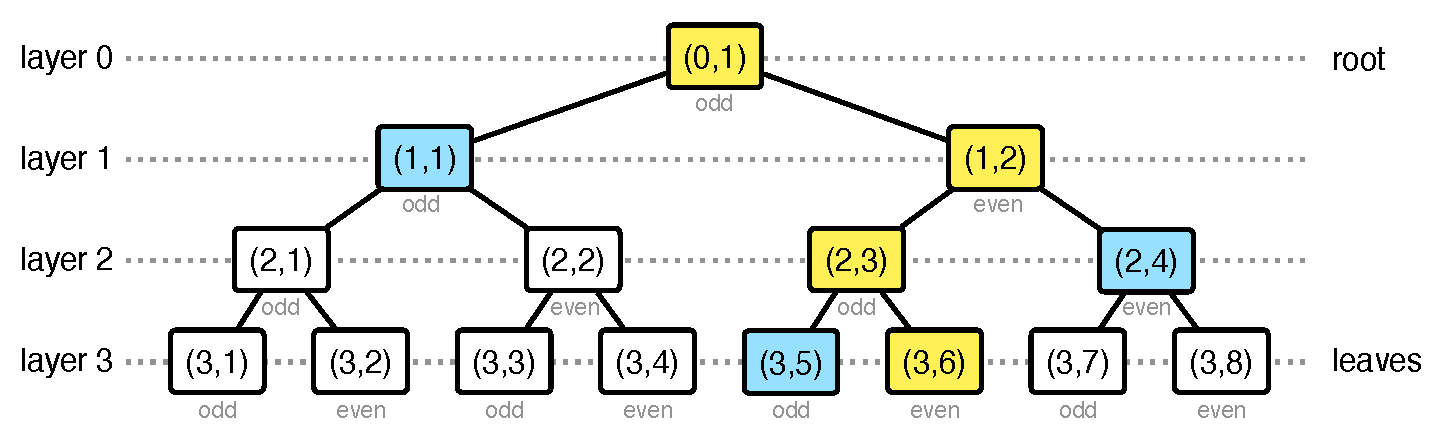
\includegraphics[width=0.75\textwidth]{\FigureFolder/tree-diagram}
\caption[The binary tree graph $\MTGraph_{8}$.]{Diagram of the binary tree graph $\MTGraph_{8}$. The vertices highlighted in yellow are $\MTPath(6) = \big( (3,6),(2,3),(1,2),(0,1) \big)$ and the vertices highlighted in blue are $\MTCoPath(6) = \big( (3,5),(2,4),(1,1) \big)$. For example, $\MTPathIndex{6}{1}=(1,2)$ and $\MTPathCoIndex{6}{1}=(1,1)$.}
\label{figure:tree-diagram}
\end{figure}

\parhead{Construction}
We describe each of the algorithms in the Merkle commitment scheme $\MTSymbol$.
\begin{itemize}[leftmargin=*]

  \item $\MTCommit^{\ROFunction}(\MTMessageVector) \to (\MTCommitment,\MTTrapdoor)$
  \begin{enumerate}[nolistsep]
    \item \label{step:mt-sample-salts}
    For each message location $\MTMessageIndex = 1,\dots,\MTMessageLength$:
    \begin{itemize}[nolistsep]
      \item sample a salt $\MTSaltString_{\MTMessageIndex} \in \Bits^{\MTSaltSize}$;
      \item compute the (hiding) commitment $\MTVertexLabelByName{\MTDepth}{\MTMessageIndex} \DefineEqual \ROFunction(\MTMessageVector[\MTMessageIndex],\MTSaltString_{\MTMessageIndex}) \in \Bits^{\ROOutputSize}$.
    \end{itemize}
    \item For each layer $\MTLayer = \MTDepth-1,\dots,0$ and for each $\MTMessageIndex = 1,\dots,2^{\MTLayer}$:
    \begin{itemize}[nolistsep]
      \item compute the (non-hiding) commitment $\MTVertexLabelByName{\MTLayer}{\MTMessageIndex} \DefineEqual \ROFunction(\MTVertexLabelByName{\MTLayer+1}{2\MTMessageIndex-1},\MTVertexLabelByName{\MTLayer+1}{2\MTMessageIndex}) \in \Bits^{\ROOutputSize}$.
    \end{itemize}
    \item Set the Merkle commitment $\MTCommitment \DefineEqual \MTVertexLabelByName{0}{1}$.
    \item Set the salts $\MTSaltStrings \DefineEqual (\MTSaltString_{\MTMessageIndex})_{\MTMessageIndex \in [\MTMessageLength]}$.
    \item Set the commitments $\MTVertexLabels \DefineEqual ((\MTVertexLabelByName{\MTLayer}{\MTMessageIndex})_{\MTMessageIndex \in [2^{\MTLayer}]})_{\MTLayer=0}^{\MTDepth}$, which we can visualize in the following way:
\begin{equation*}
\MTVertexLabels
=
\begin{bmatrix}
    \MTVertexLabelByName{0}{1} & & & & & \\
    \MTVertexLabelByName{1}{1} & \MTVertexLabelByName{1}{2} & & & & \\
    \MTVertexLabelByName{2}{1} & \MTVertexLabelByName{2}{2} & \MTVertexLabelByName{2}{3} & \MTVertexLabelByName{2}{4} & & \\
    \vdots & \vdots & \vdots & \vdots & \ddots & \\
    \MTVertexLabelByName{\MTDepth}{1} & \dots & \dots & \dots & \dots & \MTVertexLabelByName{\MTDepth}{2^{\MTDepth}}
\end{bmatrix}
\enspace.
\end{equation*}
    \item Set the opening trapdoor $\MTTrapdoor \DefineEqual (\MTSaltStrings,\MTVertexLabels)$.
    \item Output $(\MTCommitment,\MTTrapdoor)$.
  \end{enumerate}

  Informally, this algorithm first commits to each message entry via a basic commitment scheme (the one discussed in \Cref{chapter:basic-commitment}) and labels the leaves of the binary tree with these commitments, and then recursively labels every vertex in the tree with the hash of the labels of its two children.

  \item $\MTOpen^{\ROFunction}(\MTTrapdoor, \MTMessageIndexSet) \to \MTProof$
  \begin{enumerate}[nolistsep]
    \item For every $\MTMessageIndex \in \MTMessageIndexSet$, set the authentication path for location $\MTMessageIndex$:
\begin{equation}
\label{equation:mt-authpath-structure}
\MTAuthPath_{\MTMessageIndex}
\DefineEqual
\big(
  \MTSaltString_{\MTMessageIndex}
  ,
  (\MTVertexLabelByCoPath{\MTMessageIndex}{\MTLayer})_{\MTLayer \in \{1,\dots,\MTDepth\}}
\big)
\enspace.
\end{equation}
    \item Output the opening proof $\MTProof \DefineEqual (\MTAuthPath_{\MTMessageIndex})_{\MTMessageIndex \in \MTMessageIndexSet}$.
  \end{enumerate}

  Informally, this algorithm includes an authentication path for each opened location. An authentication for a location includes the salt for that location, as well as the values assigned to siblings of vertices from that leaf location to the root.

  \item $\MTCheck^{\ROFunction}(\MTCommitment,\MTMessageIndexSet,\MTMessageSubVector,\MTProof) \to b$
  \begin{enumerate}[nolistsep]
    \item Parse $\MTProof$ as $(\MTAuthPath_{\MTMessageIndex})_{\MTMessageIndex \in \MTMessageIndexSet}$.
    \item For every $\MTMessageIndex \in \MTMessageIndexSet$, check that $\MTAuthPath_{\MTMessageIndex}$ authenticates the value $\MTMessageSubVector[\MTMessageIndex] \in \MTAlphabet$ as the $\MTMessageIndex$-th opening relative to the Merkle commitment $\MTCommitment \in \Bits^{\ROOutputSize}$ by computing $(\MTVertexLabelByPath{\MTMessageIndex}{\MTLayer})_{\MTLayer \in \{0,1,\dots,\MTDepth\}}$:
    \begin{enumerate}[nolistsep]
      \item \label{step:mtcheck:leaf-query}
      compute the commitment $\MTVertexLabelByName{\MTDepth}{\MTMessageIndex} \DefineEqual \ROFunction(\MTMessageSubVector[\MTMessageIndex],\MTSaltString_{\MTMessageIndex})$;
      \item compute the commitments $(\MTVertexLabelByPath{\MTMessageIndex}{\MTLayer})_{\MTLayer \in \{0,1,\dots,\MTDepth-1\}}$ as follows:\\ for each layer $\MTLayer = \MTDepth-1,\dots,1,0$:
      \begin{itemize}[nolistsep]
        \item if $\MTPathIndex{\MTMessageIndex}{\MTLayer+1}$ is an odd vertex then set $\MTLeftVertexLabel \DefineEqual \MTVertexLabelByPath{\MTMessageIndex}{\MTLayer+1}$ and $\MTRightVertexLabel \DefineEqual \MTVertexLabelByCoPath{\MTMessageIndex}{\MTLayer+1}$;
        \item if $\MTPathIndex{\MTMessageIndex}{\MTLayer+1}$ is an even vertex then set $\MTLeftVertexLabel \DefineEqual \MTVertexLabelByCoPath{\MTMessageIndex}{\MTLayer+1}$ and $\MTRightVertexLabel \DefineEqual \MTVertexLabelByPath{\MTMessageIndex}{\MTLayer+1}$;
        \item \label{step:mtcheck:internal-query}
        compute the commitment $\MTVertexLabelByPath{\MTMessageIndex}{\MTLayer} \DefineEqual \ROFunction(\MTLeftVertexLabel,\MTRightVertexLabel)$.
      \end{itemize}
      \item check that $\MTCommitment = \MTVertexLabelByName{0}{1}$.
    \end{enumerate}
  \end{enumerate}

  Informally, this algorithm checks the authentication path from each location. Checking an authentication path involves re-computing the values assigned to vertices from the leaf vertex of the location to the root vertex, and checking that the resulting root value equals the given Merkle commitment. Note that
\begin{equation}
\label{equation:mt-check-and-for-each-location}
\MTCheck^{\ROFunction}(\MTCommitment,\MTMessageIndexSet,\MTMessageSubVector,\MTProof)
=
\idxland{\MTMessageIndex \in \MTMessageIndexSet}\, \MTCheck^{\ROFunction}(\MTCommitment,\MTMessageIndex,\MTMessageSubVector[\MTMessageIndex],\MTAuthPath_{\MTMessageIndex})
\enspace.
\end{equation}
Above we slightly abuse notation in that we drop the set notation when $\MTCheck$ receives a single location and a single corresponding authentication path.

\end{itemize}

\parhead{Efficiency}
We discuss the efficiency of each algorithm.
\begin{itemize}

  \item The algorithm $\MTCommit$ makes $\MTMessageLength$ queries of size $\log\Cardinality{\MTAlphabet}+\MTSaltSize$, and $\sum_{\MTLayer \in [\MTDepth]} \MTMessageLength/2^{\MTDepth-\MTLayer-1} \leq \MTMessageLength$ queries of size $2\ROOutputSize$. The output Merkle commitment $\MTCommitment$ has size $\ROOutputSize$ and opening trapdoor $\MTTrapdoor$ has size $\MTSaltSize \MTMessageLength + 2\MTMessageLength\ROOutputSize$.

  \item The algorithm $\MTOpen$ makes no oracle calls, and simply includes in the opening proof an authentication path for each index in the set $\MTMessageIndexSet$. An authentication path has size $\MTSaltSize + \MTDepth\ROOutputSize$, since it includes the salt and a hash per layer. Hence an opening proof consists of $\Cardinality{\MTMessageIndexSet} \cdot (\MTSaltSize + \MTDepth\ROOutputSize)$ bits. The path-pruning optimization discussed in \Cref{section:compressing-opening-proof} reduces the size of an opening proof.

  \item The algorithm $\MTCheck$, for each location in the set $\MTMessageIndexSet$, makes one query of size $\log\Cardinality{\MTAlphabet}+\MTSaltSize$ and $\MTDepth$ queries of size $2\ROOutputSize$. The total number of queries is $\Cardinality{\cup_{\MTMessageIndex \in \MTMessageIndexSet}\MTPath(\MTMessageIndex)}$ (there may be duplicates).

\end{itemize}

\begin{figure}[htp!]
\centering
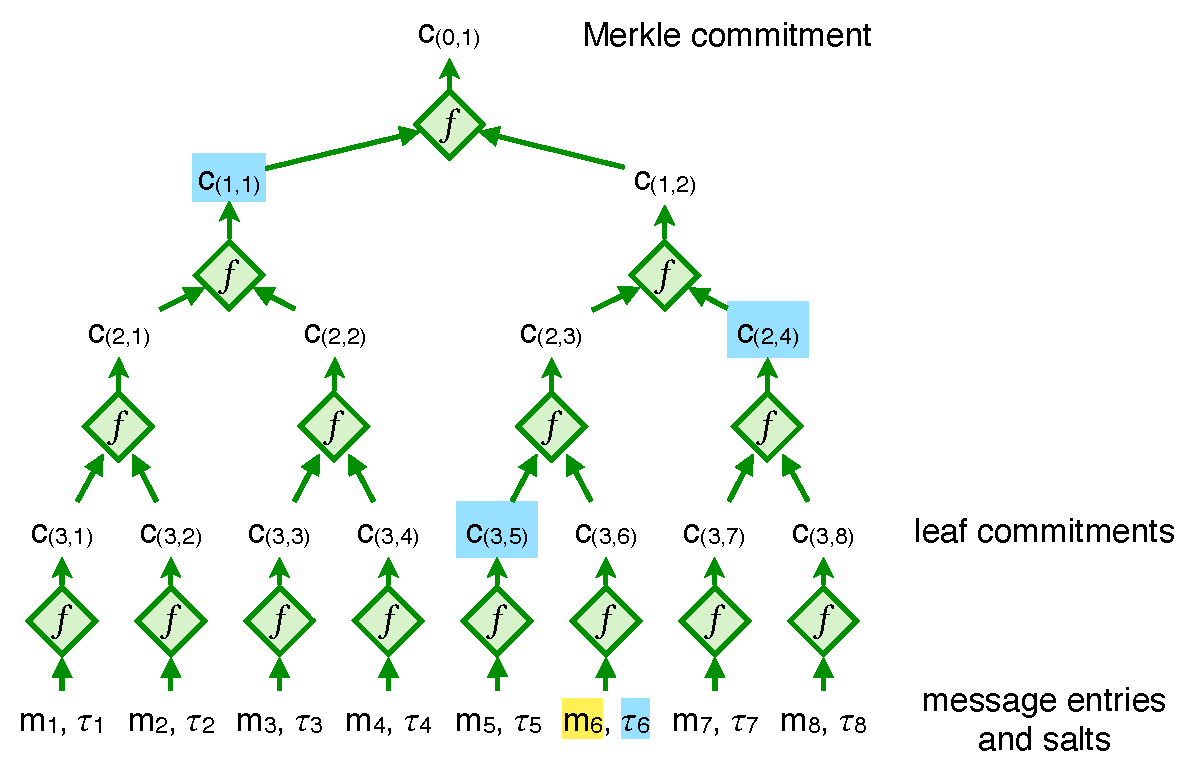
\includegraphics[width=0.7\textwidth]{\FigureFolder/mt-diagram}
\caption[Computation of $\MTCommit$ for $\MTMessageLength=8$.]{Diagram of the computation in $\MTCommit$ to produce a Merkle commitment for a message of length $\MTMessageLength=8$. Moreover, highlighted in blue is the information included in an opening proof $\MTProof$ for the $6$-th entry of the message (which is highlighted in yellow): the salt $\MTSaltString_{6}$ and the commitments $(\MTVertexLabel_{(3,5)},\MTVertexLabel_{(2,4)},\MTVertexLabel_{(1,1)})$ that correspond to the copath $\MTCoPath(6) = \big( (3,5),(2,4),(1,1) \big)$.}
\label{figure:mt-diagram}
\end{figure}

\begin{remark}[no privacy]
\label{remark:mt-no-privacy}
If no privacy is desired then the construction of $\MTSymbol$ simplifies as follows:
\begin{inparaenum}[(i)]
  \item $\MTSaltSize = 0$ (no salts are sampled);
  \item in $\MTCommit$, set $\MTVertexLabelByName{\MTDepth}{\MTMessageIndex} \DefineEqual \MTMessageVector[\MTMessageIndex]$ for each $\MTMessageIndex \in [\MTMessageLength]$ (instead of committing first by setting $\MTVertexLabelByName{\MTDepth}{\MTMessageIndex} \DefineEqual \ROFunction(\MTMessageVector[\MTMessageIndex],\MTSaltString_{\MTMessageIndex})$) and then the opening trapdoor $\MTTrapdoor$ does not include any salts;
  \item in $\MTOpen$, each authentication path $\MTAuthPath_{\MTMessageIndex}$ does not include any salt;
  \item in $\MTCheck$, similarly to $\MTCommit$, simply set $\MTVertexLabelByName{\MTDepth}{\MTMessageIndex} \DefineEqual \MTMessageVector[\MTMessageIndex]$ for each $\MTMessageIndex \in \MTMessageIndexSet$ (in \Cref{step:mtcheck:leaf-query}).
\end{inparaenum}
The efficiency measures are correspondingly reduced by setting $\MTSaltSize=0$.
\end{remark}

\begin{remark}[recomputing the tree]
\label{remark:recomputing-the-tree}
Some information from $\MTTrapdoor$ can be omitted (thereby reducing its size) at the expense of additional computation by $\MTOpen$. Specifically, the commitments $((\MTVertexLabelByName{\MTLayer}{\MTMessageIndex})_{\MTMessageIndex \in [2^{\MTLayer}]})_{\MTLayer=1}^{\MTDepth-1}$ in the opening trapdoor $\MTTrapdoor$ can be derived via at most $\MTMessageLength$ random oracle calls from the commitments $(\MTVertexLabelByName{\MTDepth}{\MTMessageIndex})_{\MTMessageIndex \in [\MTMessageLength]}$, and thus could be omitted from $\MTTrapdoor$. In such a case, $\MTOpen$ would have to query the random oracle to (re)derive the commitments required to construct the relevant authentication paths. In fact, $(\MTVertexLabelByName{\MTDepth}{\MTMessageIndex})_{\MTMessageIndex \in [\MTMessageLength]}$ can themselves be derived from the message $\MTMessageVector$ and salts $\MTSaltStrings$ via $\MTMessageLength$ random oracle calls; so one could even set $\MTTrapdoor \DefineEqual (\MTMessageVector,\MTSaltStrings)$, which may be advantageous if $\log\Cardinality{\MTAlphabet}$ is smaller than $\ROOutputSize$. These can be useful time-memory tradeoffs in practice.
\end{remark}

\begin{remark}[local updates]
\label{remark:locally-updatable}
Merkle commitments are \emph{locally updatable}, which is a useful feature in many applications (though we do not explore it further within the context of succinct arguments). Suppose you are given a Merkle commitment $\MTCommitment$ of a message $\MTMessageVector$, and you want to update it to be a Merkle commitment $\MTCommitment'$ of a message $\MTMessageVector'$ where $\MTMessageVector'$ is equal to $\MTMessageVector$ except for the $\MTMessageIndex$-th entry. There is no need to recompute the tree from scratch: one only needs to recompute the commitments for the vertices on the paths $\MTPath(\MTMessageIndex)$ and $\MTCoPath(\MTMessageIndex)$, while the other commitments remain unchanged. The work needed for this update is proportional to the depth of the tree (which is logarithmic in the message length) rather than the message length.
\end{remark}

\begin{remark}[$\MTMessageLength=1$]
\label{remark:mt-message-length-one}
The message length $\MTMessageLength=1$ is a power of $2$, and in this case the binary tree $\MTGraph_{\MTMessageLength}$ contains a single vertex, the root vertex. In this degenerate case ($\MTMessageLength=1$) the Merkle commitment $\MTSymbol$ happens to equal the basic commitment $\CMSymbol$.
\end{remark}

\begin{remark}[any message length]
\label{remark:mt-any-message-length}
The description of the Merkle commitment scheme $\MTSymbol$ given above involves a binary tree over $\MTMessageLength$ leaves, where $\MTMessageLength$ is the number of entries in the message vector. Notationally it is far simpler to describe and analyze the case when $\MTMessageLength$ is a power of $2$ (which we assume throughout this chapter) because the internal vertices in the binary tree can be labeled via a simple naming scheme and, more generally, all paths from the root vertex to a leaf vertex \DoQuote{look the same}. But how do Merkle commitment schemes work when $\MTMessageLength$ is not a power of $2$?

One option is to pad the message with dummy values (an arbitrary symbol from the alphabet $\MTAlphabet$) until the padded message length reaches a power of $2$; this, at most, doubles the length relative to the original (unpadded) message. All security analyses of this chapter hold for the padded message, and in particular for the original (unpadded) message.

While the padding is not expensive, there are cheaper solutions that involve binary trees with precisely $\MTMessageLength$ leaves (without using any padding). This optimization is explained in \Cref{section:any-message-length}.
\end{remark}

\begin{remark}[other arities]
\label{remark:other-arities}
The description above involves a perfect \emph{binary} tree. However the construction of a Merkle commitment scheme and the properties that we study (completeness, binding, extractability, hiding) directly extend to perfect trees of any arity. (In fact, see \Cref{section:any-message-length} for a \emph{generalized} Merkle commitment scheme that is defined for \emph{any tree}.)  If the tree has arity $\MTArity \geq 2$ then each authentication path contains $\MTArity-1$ vertices per layer rather than $1$, and the number of layers in the tree is $\log_{\MTArity} \MTMessageLength$ rather than $\log_{2} \MTMessageLength$. Larger arities are usually not advantageous for the size of opening proofs (the tree has fewer layers but there are more sibling vertices for an overall bigger opening proof size), though there may be other reasons to consider trees of higher arity (e.g., fewer calls to the random oracle).
\end{remark}

%%%%%%%%%%%%%%%%%%%%%%%%%%%%%%%%%%%%%%%%%%%%%%%%%%%%%%%%%%%%%%%%%%%%%%%%%%%%%%%
%%%%%%%%%%%%%%%%%%%%%%%%%%%%%%%%%%%%%%%%%%%%%%%%%%%%%%%%%%%%%%%%%%%%%%%%%%%%%%%
%%%%%%%%%%%%%%%%%%%%%%%%%%%%%%%%%%%%%%%%%%%%%%%%%%%%%%%%%%%%%%%%%%%%%%%%%%%%%%%
\section{Completeness}
\label{section:merkle-commitment-completeness}

We prove that $\MTCommit$ has \emph{completeness}, namely, if the algorithms of the Merkle commitment scheme are used as intended then validity checks always pass. In more detail, $\MTCommit$ can be used to commit to any message vector, and $\MTOpen$ can be used to open any subset of locations of the message vector in such a way that the resulting opening proof is accepted by $\MTCheck$.

\begin{lemma}[$\MTSymbol$ is complete]
\label{lemma:mt-completeness}
Let $\MTSymbol \DefineEqual \MTConstructor{\ROOutputSize}{\MTAlphabet}{\MTMessageLength}{\MTSaltSize}$. For every adversary $\MTAdversary$,
\begin{equation*}
\Pr\left[
\MTCheck^{\ROFunction}(\MTCommitment,\MTMessageIndexSet,\MTMessageVector[\MTMessageIndexSet],\MTProof)=1
\GivenExperiment
\StateExperiment{
\ROFunction \gets \RODistribution{\ROOutputSize} \\
(\MTMessageVector,\MTMessageIndexSet) \gets \MTAdversary^{\ROFunction} \\
(\MTCommitment,\MTTrapdoor) \gets \MTCommit^{\ROFunction}(\MTMessageVector) \\
\MTProof \gets \MTOpen^{\ROFunction}(\MTTrapdoor, \MTMessageIndexSet)
}
\right]
= 1
\enspace.
\end{equation*}
\end{lemma}

A formal proof of this lemma would involve analyzing each step of each Merkle commitment algorithm in order to establish that all validity checks pass. This would be not provide useful insights. Instead we sketch the proof at high level to provide the main intuition.

Fix an arbitrary choice of oracle $\ROFunction \in \RODistribution{\ROOutputSize}$, message $\MTMessageVector \in \MTAlphabet^{\MTMessageLength}$, and subset $\MTMessageIndexSet \subseteq [\MTMessageLength]$.

The algorithm $\MTCommit$ computes the Merkle commitment for $\MTMessageVector$ by first committing to each entry of $\MTMessageVector$ (using a random salt $\MTSaltString_{\MTMessageIndex}$ for each message entry $\MTMessageVector[\MTMessageIndex]$), then pairwise hashes the resulting list to halve its size, and so on, until it obtains a single output $\MTCommitment$; the trapdoor $\MTTrapdoor$ is set to contain all the salts that were sampled and all the commitments $\MTVertexLabels \DefineEqual ((\MTVertexLabelByName{\MTLayer}{\MTMessageIndex})_{\MTMessageIndex \in [2^{\MTLayer}]})_{\MTLayer=0}^{\MTDepth}$ that were computed.

Subsequently, the algorithm $\MTOpen$ includes in the opening proof $\MTProof$ an authentication path $\MTAuthPath_{\MTMessageIndex} = \big(\MTSaltString_{\MTMessageIndex},(\MTVertexLabelByCoPath{\MTMessageIndex}{\MTLayer})_{\MTLayer \in \{1,\dots,\MTDepth\}}\big)$ for each index $\MTMessageIndex$ in the subset $\MTMessageIndexSet$.

The algorithm $\MTCheck$, for each index $\MTMessageIndex$ in the subset $\MTMessageIndexSet$, checks that the authentication path $\MTAuthPath_{\MTMessageIndex}$ is valid relative to the Merkle commitment $\MTCommitment$, index $\MTMessageIndex$, and value $\MTMessageSubVector[\MTMessageIndex]$. The check for each authentication path succeeds because $\MTOpen$ constructed that path by including the correct salt and the correct commitments, which will lead $\MTCheck$ to recompute the same value for the root vertex as $\MTCommitment$.



%%%%%%%%%%%%%%%%%%%%%%%%%%%%%%%%%%%%%%%%%%%%%%%%%%%%%%%%%%%%%%%%%%%%%%%%%%%%%%%
%%%%%%%%%%%%%%%%%%%%%%%%%%%%%%%%%%%%%%%%%%%%%%%%%%%%%%%%%%%%%%%%%%%%%%%%%%%%%%%
%%%%%%%%%%%%%%%%%%%%%%%%%%%%%%%%%%%%%%%%%%%%%%%%%%%%%%%%%%%%%%%%%%%%%%%%%%%%%%%
\section{Collision lemma}
\label{section:merkle-commitment-collision-lemma}

We formulate and prove a \emph{collision lemma} for Merkle commitments, which is a basic security property that we use in later sections. Informally, the lemma states that authenticating different values for the same leaf in a Merkle commitment leads to a collision in the random oracle. Stating this property precisely, however, requires some care. The discussion below takes an incremental approach by considering simpler types of collision lemmas. First, we describe a collision lemma for the basic commitment scheme $\CMSymbol$ in \Cref{chapter:basic-commitment}. Second, we describe a special case of the collision lemma for Merkle commitment schemes. Third, and finally, we describe the (general) collision lemma for Merkle commitment schemes.

\parhead{Starting simple: collisions in $\CMSymbol$}
Consider the basic commitment scheme $\CMSymbol$ in \Cref{chapter:basic-commitment}, whose checking algorithm $\CMCheck$ simply consists of checking a query-answer pair of the random oracle: $\CMCheck^{\ROFunction}(\CMCommitment,\CMMessage,\CMSaltString)=1$ if and only if $\CMCommitment = \ROFunction(\CMMessage,\CMSaltString)$. Consider a commitment $\CMCommitment$ and two message-salt pairs, $(\CMMessage_{0},\CMSaltString_{0})$ and $(\CMMessage_{1},\CMSaltString_{1})$. Suppose that both pairs are valid openings of the commitment, that is, $\CMCheck^{\ROFunction}(\CMCommitment,\CMMessage_{0},\CMSaltString_{0})=1$ and $\CMCheck^{\ROFunction}(\CMCommitment,\CMMessage_{1},\CMSaltString_{1})=1$. By the definition of $\CMCheck$, these conditions are equivalent to $\CMCommitment = \ROFunction(\CMMessage_{0},\CMSaltString_{0})$ and $\CMCommitment = \ROFunction(\CMMessage_{1},\CMSaltString_{1})$, from which we deduce that $\ROFunction(\CMMessage_{0},\CMSaltString_{0})=\ROFunction(\CMMessage_{1},\CMSaltString_{1})$. This tells us that if either $\CMMessage_{0} \neq \CMMessage_{1}$ (the messages are distinct) or $\CMSaltString_{0} \neq \CMSaltString_{1}$ (the salts are distinct) then the two executions of $\CMCheck$ on the two inputs result in a collision for $\ROFunction$. Thus, in $\CMSymbol$, \emph{opening the same commitment either via two different messages or via two different salts leads to a collision}. We can summarize this property as a \DoQuote{collision lemma for $\CMSymbol$} via the following implication:
\begin{equation*}
\left[
\begin{array}{l}
\big(
\CMMessage_{0} \neq \CMMessage_{1}
\lor
\CMSaltString_{0} \neq \CMSaltString_{1}
\big) \\
\land \;\CMCheck^{\ROFunction}(\CMCommitment,\CMMessage_{0},\CMSaltString_{0})=1 \\
\land \;\CMCheck^{\ROFunction}(\CMCommitment,\CMMessage_{1},\CMSaltString_{1})=1
\end{array}
\right]
\Rightarrow\;
\left[
\begin{array}{c}
\text{$(\CMMessage_{0},\CMSaltString_{0})$ and $(\CMMessage_{1},\CMSaltString_{1})$} \\
\text{are a collision for $\ROFunction$}
\end{array}
\right]
\enspace.
\end{equation*}

\parhead{What about $\MTSymbol$?}
We wish to derive a similar lemma for the Merkle commitment scheme $\MTSymbol$. The challenge is that messages in $\MTSymbol$ can be opened at subsets of locations (rather than only at all locations), which complicates the assumptions under which a collision can be proved to exist. Moreover, the algorithm $\MTCheck$, which validates the corresponding opening proofs, involves a more complex computation. In particular, the computation involves multiple queries to the random oracle (rather than one query as in $\CMSymbol$), and arguing that a collision exists in the relevant query-answer traces will involve a delicate case analysis. We tackle this additional complexity by first analyzing a special case and then analyzing the general case.

\parhead{Special case: opening a single leaf}
As a warmup we consider the special case where we only consider opening proofs for a single leaf. In other words, we consider computations for $\MTCheck^{\ROFunction}(\MTCommitment,\MTMessageIndexSet,\MTMessageSubVector,\MTProof)$ where the set $\MTMessageIndexSet = \{\MTMessageIndex\}$ is a singleton and so:
\begin{inparaenum}[(i)]
  \item $\MTMessageSubVector$ is a vector consisting of a single entry $\MTMessageEntry$ in $\MTAlphabet$; and
  \item $\MTProof$ consists of a single authentication path $\MTAuthPath$.
\end{inparaenum}

Consider a Merkle commitment $\MTCommitment$ and position $\MTMessageIndex \in [\MTMessageLength]$, and two openings: a claimed value $\MTMessageEntry_{0} \in \MTAlphabet$ and corresponding authentication path $\MTAuthPath_{0}$, and another claimed value $\MTMessageEntry_{1} \in \MTAlphabet$ and corresponding authentication path $\MTAuthPath_{1}$. Suppose that both openings are valid, that is, $\MTCheck^{\ROFunction}(\MTCommitment,\MTMessageIndex,\MTMessageEntry_{0},\MTAuthPath_{0})=1$ and $\MTCheck^{\ROFunction}(\MTCommitment,\MTMessageIndex,\MTMessageEntry_{1},\MTAuthPath_{1})=1$. Intuitively, since the two computations share the same Merkle commitment $\MTCommitment$, if $\MTMessageEntry_{0} \neq \MTMessageEntry_{1}$ then the two random oracle computations \DoQuote{collide} at some layer of the binary tree in order to eventually lead to the same Merkle commitment $\MTCommitment$ at the root of the tree. The collision is either at a leaf commitment, or at an internal commitment; see \Cref{figure:mt-collision-lemma} for an example. In fact, we can prove that the same is true even if $\MTMessageEntry_{0} = \MTMessageEntry_{1}$ and $\MTAuthPath_{0} \neq \MTAuthPath_{1}$.

\begin{figure}[htp!]
\centering
\begin{subfigure}[b]{0.4\textwidth}
\centering
  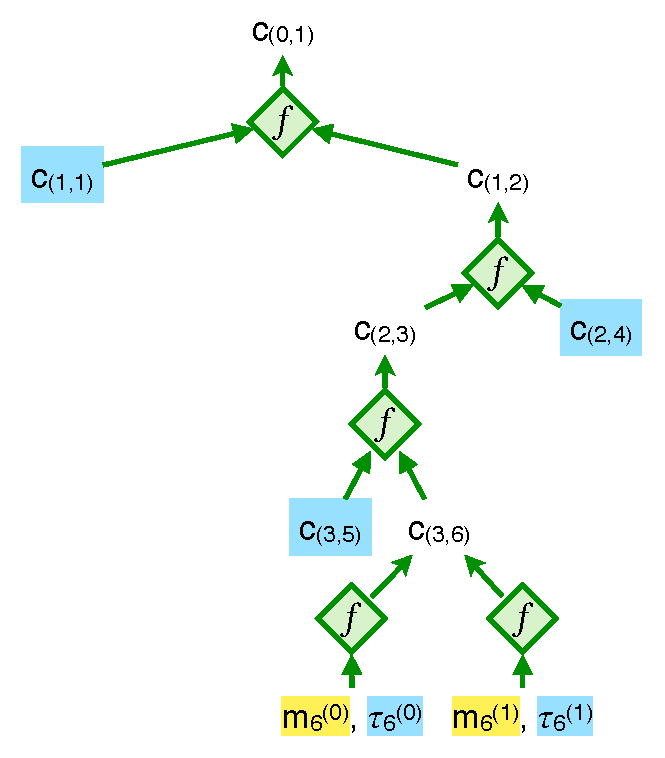
\includegraphics[width=\textwidth]{\FigureFolder/mt-collision-lemma-diagram-1}
  \caption{}
  \label{figure:mt-collision-lemma-1}
\end{subfigure}
\quad
\begin{subfigure}[b]{0.55\textwidth}
  \centering
  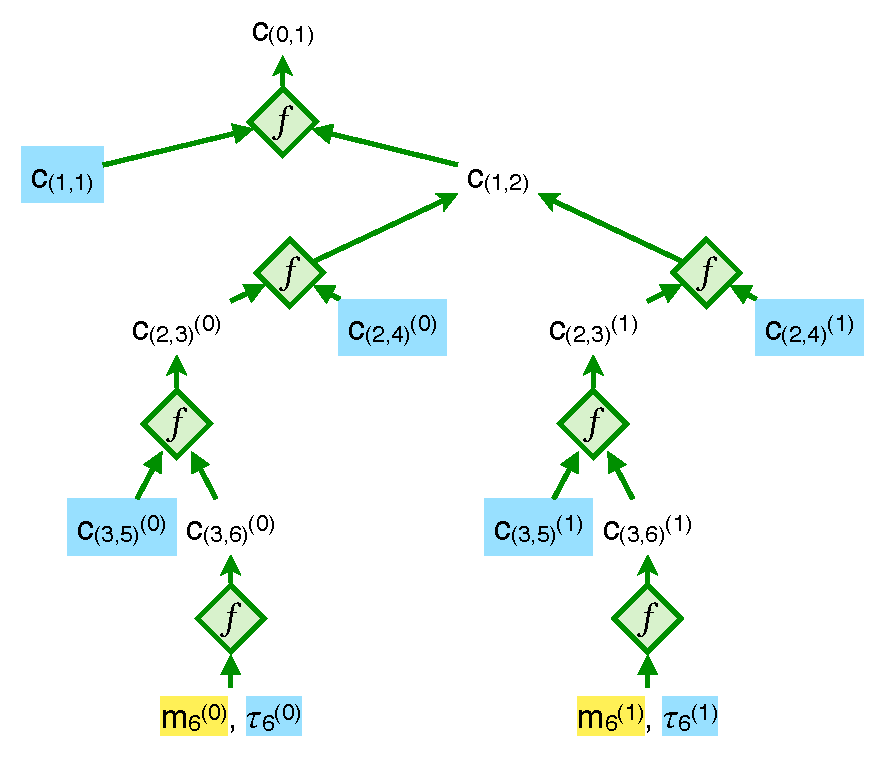
\includegraphics[width=\textwidth]{\FigureFolder/mt-collision-lemma-diagram-2}
  \caption{}
  \label{figure:mt-collision-lemma-2}
\end{subfigure}
\caption[Collision between two authentication paths.]{Example of a collision for two paths that authenticate two different values for the $6$-th entry (out of $8$ entries). There are two cases: in the left, a collision at a leaf commitment; and, on the right, a collision at an internal commitment.}
\label{figure:mt-collision-lemma}
\end{figure}

More precisely, the collision involves a query from the query-answer trace $\ROHonestTrace_{0}$ of the computation $\MTCheck^{\ROFunction}(\MTCommitment,\MTMessageIndex,\MTMessageEntry_{0},\MTAuthPath_{0})$ and a query from the query-answer trace $\ROHonestTrace_{1}$ of the computation $\MTCheck^{\ROFunction}(\MTCommitment,\MTMessageIndex,\MTMessageEntry_{1},\MTAuthPath_{1})$.

Note that here it is necessary for the two openings to be about the same position $\MTMessageIndex$. This is because it is possible to open two different positions via two different values (or different authentication paths) without causing collisions. Indeed, this would happen for most choices of random oracle for a message with different values.

We formally state and prove this below.

\begin{lemma}
\label{lemma:simple-mt-colliding-paths}
Let $\MTSymbol \DefineEqual \MTConstructor{\ROOutputSize}{\MTAlphabet}{\MTMessageLength}{\MTSaltSize}$. Fix arbitrary choices of oracle $\ROFunction \in \RODistribution{\ROOutputSize}$ and:
\begin{inparaenum}[\emptylabel]
  \item a Merkle commitment $\MTCommitment \in \Bits^{\ROOutputSize}$;
  \item an index $\MTMessageIndex \in [\MTMessageLength]$;
  \item message entries $\MTMessageEntry_{0},\MTMessageEntry_{1} \in \MTAlphabet$; and
  \item authentication paths $\MTAuthPath_{0},\MTAuthPath_{1}$.
\end{inparaenum}
For $b \in \Bits$, let $\ROHonestTrace_{b}$ be the query-answer trace of $\MTCheck^{\ROFunction}(\MTCommitment,\MTMessageIndex,\MTMessageEntry_{b},\MTAuthPath_{b})$. Then the following implication holds:
\begin{equation}
\label{equation:simple-mt-colliding-paths}
\left[
\begin{array}{l}
\big(
\MTMessageEntry_{0} \neq \MTMessageEntry_{1}
\lor
\MTAuthPath_{0} \neq \MTAuthPath_{1}
\big) \\
\land \;\MTCheck^{\ROFunction}(\MTCommitment,\MTMessageIndex,\MTMessageEntry_{0},\MTAuthPath_{0})=1 \\
\land \;\MTCheck^{\ROFunction}(\MTCommitment,\MTMessageIndex,\MTMessageEntry_{1},\MTAuthPath_{1})=1
\end{array}
\right]
\Rightarrow\;
\left[
\begin{array}{c}
\exists\,
(\ROQuery_{0},\ROAnswer_{0}) \in \ROHonestTrace_{0}
,
(\ROQuery_{1},\ROAnswer_{1}) \in \ROHonestTrace_{1}
\\
\text{with $\ROQuery_{0} \neq \ROQuery_{1}$}
\text{ such that } \ROAnswer_{0}=\ROAnswer_{1}
\end{array}
\right]
\enspace.
\end{equation}
\end{lemma}

\begin{proof}
Fix $b \in \Bits$. The authentication path $\MTAuthPath_{b}$ for index $\MTMessageIndex$ has the following structure:
\begin{equation*}
\MTAuthPath_{b}
=
\Big(
  \MTSaltString_{\MTMessageIndex}^{(b)}
  ,
  (\MTVertexLabelByCoPath{\MTMessageIndex}{\MTLayer}^{(b)})_{\MTLayer \in \{1,\dots,\MTDepth\}}
\Big)
\enspace,
\end{equation*}
where $\MTSaltString_{\MTMessageIndex}^{(b)}$ is a Merkle salt and $(\MTVertexLabelByCoPath{\MTMessageIndex}{\MTLayer}^{(b)})_{\MTLayer \in \{1,\dots,\MTDepth\}}$ are commitments labeling vertices in $\MTCoPath(\MTMessageIndex)$.

Moreover, the computation $\MTCheck^{\ROFunction}(\MTCommitment,\MTMessageIndex,\MTMessageEntry_{b},\MTAuthPath_{b})$ leads to a query-answer trace $\ROHonestTrace_{b}$ consisting of $\MTDepth+1$ query-answer pairs. The answers in $\ROHonestTrace_{b}$ are denoted
\begin{equation*}
(\MTVertexLabelByPath{\MTMessageIndex}{\MTLayer}^{(b)})_{\MTLayer \in \{0,1,\dots,\MTDepth\}}
\enspace.
\end{equation*}
Finally, $\MTCheck^{\ROFunction}(\MTCommitment,\MTMessageIndex,\MTMessageEntry_{b},\MTAuthPath_{b}) = 1$ implies that $\MTCommitment = \MTVertexLabelByName{0}{1}^{(b)}$.

In particular, we deduce that $\MTVertexLabelByName{0}{1}^{(0)}=\MTVertexLabelByName{0}{1}^{(1)}$.

We consider two cases.
\begin{itemize}

  \item \emph{Case 1: there exists $\MTLayer \in [\MTDepth]$ such that $\MTVertexLabelByPath{\MTMessageIndex}{\MTLayer}^{(0)} \neq \MTVertexLabelByPath{\MTMessageIndex}{\MTLayer}^{(1)}$ or $\MTVertexLabelByCoPath{\MTMessageIndex}{\MTLayer}^{(0)} \neq \MTVertexLabelByCoPath{\MTMessageIndex}{\MTLayer}^{(1)}$.}

Let $\MTLayer$ be the minimal index satisfying this condition.
\begin{itemize}[nolistsep]
  \item If $\MTPathIndex{\MTMessageIndex}{\MTLayer}$ is an odd vertex then for $b \in \Bits$ set $(\MTLeftVertexLabel^{(b)},\MTRightVertexLabel^{(b)}) \DefineEqual (\MTVertexLabelByPath{\MTMessageIndex}{\MTLayer}^{(b)},\MTVertexLabelByCoPath{\MTMessageIndex}{\MTLayer}^{(b)})$.
  \item If $\MTPathIndex{\MTMessageIndex}{\MTLayer}$ is an even vertex then for $b \in \Bits$ set $(\MTLeftVertexLabel^{(b)},\MTRightVertexLabel^{(b)}) \DefineEqual (\MTVertexLabelByCoPath{\MTMessageIndex}{\MTLayer}^{(b)},\MTVertexLabelByPath{\MTMessageIndex}{\MTLayer}^{(b)})$.
\end{itemize}
For $b \in \Bits$ the pair $(\MTLeftVertexLabel^{(b)},\MTRightVertexLabel^{(b)})$ is a query in $\ROHonestTrace_{b}$ (see \Cref{step:mtcheck:internal-query} in the description of $\MTCheck$).

These two queries are a collision for $\ROFunction$ due to the following.
\begin{itemize}[nosep]

  \item $(\MTLeftVertexLabel^{(0)},\MTRightVertexLabel^{(0)}) \neq (\MTLeftVertexLabel^{(1)},\MTRightVertexLabel^{(1)})$. \\ This follows since $\MTVertexLabelByPath{\MTMessageIndex}{\MTLayer}^{(0)} \neq \MTVertexLabelByPath{\MTMessageIndex}{\MTLayer}^{(1)}$ or $\MTVertexLabelByCoPath{\MTMessageIndex}{\MTLayer}^{(0)} \neq \MTVertexLabelByCoPath{\MTMessageIndex}{\MTLayer}^{(1)}$.

  \item $\ROFunction(\MTLeftVertexLabel^{(0)},\MTRightVertexLabel^{(0)})=\ROFunction(\MTLeftVertexLabel^{(1)},\MTRightVertexLabel^{(1)})$. \\ This follows since $\MTVertexLabelByPath{\MTMessageIndex}{\MTLayer-1}^{(0)} = \ROFunction(\MTLeftVertexLabel^{(0)},\MTRightVertexLabel^{(0)})$, $\MTVertexLabelByPath{\MTMessageIndex}{\MTLayer-1}^{(1)} = \ROFunction(\MTLeftVertexLabel^{(1)},\MTRightVertexLabel^{(1)})$, and $\MTVertexLabelByPath{\MTMessageIndex}{\MTLayer-1}^{(0)} = \MTVertexLabelByPath{\MTMessageIndex}{\MTLayer-1}^{(1)}$. The last equality holds because $\MTLayer$ is the minimal index satisfying the condition (and we know that $\MTVertexLabelByName{0}{1}^{(0)}=\MTVertexLabelByName{0}{1}^{(1)}$).

\end{itemize}

  \item \emph{Case 2: $\MTVertexLabelByName{\MTDepth}{\MTMessageIndex}^{(0)}=\MTVertexLabelByName{\MTDepth}{\MTMessageIndex}^{(1)}$, and $\MTMessageEntry_{0} \neq \MTMessageEntry_{1}$ or $\MTSaltString_{\MTMessageIndex}^{(0)} \neq \MTSaltString_{\MTMessageIndex}^{(1)}$.}

For $b \in \Bits$ the pair $(\MTMessageEntry_{b},\MTSaltString_{\MTMessageIndex}^{(b)})$ is a query in $\ROHonestTrace_{b}$ (see \Cref{step:mtcheck:leaf-query} in the description of $\MTCheck$).

These two queries are a collision for $\ROFunction$ due to the following.
\begin{itemize}[nosep]
  \item $(\MTMessageEntry_{0},\MTSaltString_{\MTMessageIndex}^{(0)}) \neq (\MTMessageEntry_{1},\MTSaltString_{\MTMessageIndex}^{(1)})$. This follows since $\MTMessageEntry_{0} \neq \MTMessageEntry_{1}$ or $\MTSaltString_{\MTMessageIndex}^{(0)} \neq \MTSaltString_{\MTMessageIndex}^{(1)}$.
  \item $\ROFunction(\MTMessageEntry_{0},\MTSaltString_{\MTMessageIndex}^{(0)})=\ROFunction(\MTMessageEntry_{1},\MTSaltString_{\MTMessageIndex}^{(1)})$. This follows since $\MTVertexLabelByName{\MTDepth}{\MTMessageIndex}^{(0)} = \ROFunction(\MTMessageEntry_{0},\MTSaltString_{\MTMessageIndex}^{(0)})$, $\MTVertexLabelByName{\MTDepth}{\MTMessageIndex}^{(1)} = \ROFunction(\MTMessageEntry_{1},\MTSaltString_{\MTMessageIndex}^{(1)})$, and $\MTVertexLabelByName{\MTDepth}{\MTMessageIndex}^{(0)}=\MTVertexLabelByName{\MTDepth}{\MTMessageIndex}^{(1)}$.
\end{itemize}

\end{itemize}
In either case we find a collision with one query in $\ROHonestTrace_{0}$ and the other query in $\ROHonestTrace_{1}$.

We are left to argue that the antecedent in \Cref{equation:simple-mt-colliding-paths} implies that Case 1 or Case 2 holds.

If Case 1 holds then we are done. So suppose that Case 1 does not hold, which means that $(\MTVertexLabelByPath{\MTMessageIndex}{\MTLayer}^{(0)})_{\MTLayer \in [\MTDepth]}=(\MTVertexLabelByPath{\MTMessageIndex}{\MTLayer}^{(1)})_{\MTLayer \in [\MTDepth]}$ and $(\MTVertexLabelByCoPath{\MTMessageIndex}{\MTLayer}^{(0)})_{\MTLayer \in [\MTDepth]}=(\MTVertexLabelByCoPath{\MTMessageIndex}{\MTLayer}^{(1)})_{\MTLayer \in [\MTDepth]}$ (and in particular that $\MTVertexLabelByName{\MTDepth}{\MTMessageIndex}^{(0)}=\MTVertexLabelByName{\MTDepth}{\MTMessageIndex}^{(1)}$). If $\MTMessageEntry_{0} \neq \MTMessageEntry_{1}$ then Case 2 holds. Suppose instead that $\MTAuthPath_{0} \neq \MTAuthPath_{1}$. The only way for the two authentication paths to differ in this case is for the Merkle salts to differ ($\MTSaltString_{\MTMessageIndex}^{(0)} \neq \MTSaltString_{\MTMessageIndex}^{(1)}$), in which case again Case 2 holds.
\end{proof}

\parhead{General case: opening multiple leaves}
We now consider the collision lemma for the general case, where opening proofs may authenticate multiple leaves. Consider a Merkle commitment $\MTCommitment$, as well as:
\begin{inparaenum}[\emptylabel]
  \item two index sets $\MTMessageIndexSet_{0},\MTMessageIndexSet_{1}$;
  \item two vectors $\MTMessageSubVector_{0},\MTMessageSubVector_{1}$;
  \item two opening proofs $\MTProof_{0},\MTProof_{1}$.
\end{inparaenum}
Suppose that both openings are valid, that is, $\MTCheck^{\ROFunction}(\MTCommitment,\MTMessageIndexSet_{0},\MTMessageSubVector_{0},\MTProof_{0})=1$ and $\MTCheck^{\ROFunction}(\MTCommitment,\MTMessageIndexSet_{1},\MTMessageSubVector_{1},\MTProof_{1})=1$.

Intuitively, and similarly to the case of a single leaf, if there is a position $\MTMessageIndex \in \MTMessageIndexSet_{0} \cap \MTMessageIndexSet_{1}$ such that $\MTMessageSubVector_{0}[\MTMessageIndex] \neq \MTMessageSubVector_{0}[\MTMessageIndex]$ then we can find a collision in (the union of the relevant) query-answer traces. Informally, the prior argument works applied to the authentication paths for the index $\MTMessageIndex$ in the opening proofs $\MTProof_{0}$ and $\MTProof_{1}$ (and the subset of query-answer pairs used to validate these paths).

Less obvious is the fact that we cannot expect (in general) to find a collision if $\MTProof_{0} \neq \MTProof_{1}$. This is because the two opening proofs are for potentially different index sets $\MTMessageIndexSet_{0}$ and $\MTMessageIndexSet_{1}$, and so the opening proofs can be different. Nevertheless, we can prove that if the opening proofs are for the same index set ($\MTMessageIndexSet_{0}=\MTMessageIndexSet_{1}$) and they are different ($\MTProof_{0} \neq \MTProof_{1}$) then we can find a collision.

We formally state and prove this below.

\begin{lemma}
\label{lemma:mt-colliding-paths}
Let $\MTSymbol \DefineEqual \MTConstructor{\ROOutputSize}{\MTAlphabet}{\MTMessageLength}{\MTSaltSize}$. Fix arbitrary choices of oracle $\ROFunction \in \RODistribution{\ROOutputSize}$ and:
\begin{itemize}[nolistsep]
  \item a Merkle commitment $\MTCommitment \in \Bits^{\ROOutputSize}$;
  \item a set $\MTMessageIndexSet_{0} \subseteq [\MTMessageLength]$, vector $\MTMessageSubVector_{0} \in \MTAlphabet^{\MTMessageIndexSet_{0}}$, and opening proof $\MTProof_{0}$;
  \item a set $\MTMessageIndexSet_{1} \subseteq [\MTMessageLength]$, vector $\MTMessageSubVector_{1} \in \MTAlphabet^{\MTMessageIndexSet_{1}}$, and opening proof $\MTProof_{1}$.
\end{itemize}
For $b \in \Bits$, let $\ROHonestTrace_{b}$ be the query-answer trace of $\MTCheck^{\ROFunction}(\MTCommitment,\MTMessageIndexSet_{b},\MTMessageSubVector_{b},\MTProof_{b})$. Then the following implication holds:
\begin{equation}
\label{equation:mt-colliding-paths}
\left[
\begin{array}{l}
\begin{pmatrix}
\exists\;\MTMessageIndex \in \MTMessageIndexSet_{0} \cap \MTMessageIndexSet_{1} : \MTMessageSubVector_{0}[\MTMessageIndex] \neq \MTMessageSubVector_{1}[\MTMessageIndex] \\
\text{or} \\
\MTMessageIndexSet_{0} = \MTMessageIndexSet_{1} \; \land \; \MTProof_{0} \neq \MTProof_{1}
\end{pmatrix} \\
\land \;\MTCheck^{\ROFunction}(\MTCommitment,\MTMessageIndexSet_{0},\MTMessageSubVector_{0},\MTProof_{0})=1 \\
\land \;\MTCheck^{\ROFunction}(\MTCommitment,\MTMessageIndexSet_{1},\MTMessageSubVector_{1},\MTProof_{1})=1
\end{array}
\right]
\Rightarrow\;
\left[
\begin{array}{c}
\exists\,
(\ROQuery_{0},\ROAnswer_{0}) \in \ROHonestTrace_{0}
,
(\ROQuery_{1},\ROAnswer_{1}) \in \ROHonestTrace_{1}
\\
\text{with $\ROQuery_{0} \neq \ROQuery_{1}$}
\text{ such that } \ROAnswer_{0}=\ROAnswer_{1}
\end{array}
\right]
\enspace.
\end{equation}
\end{lemma}

\begin{proof}
Fix $b \in \Bits$. The opening proof $\MTProof_{b}$ for the set $\MTMessageIndexSet_{b}$ has the following structure:
\begin{equation*}
\MTProof_{b}
=
\Big(
  \MTSaltString_{\MTMessageIndex}^{(b)}
  ,
  (\MTVertexLabelByCoPath{\MTMessageIndex}{\MTLayer}^{(b)})_{\MTLayer \in \{1,\dots,\MTDepth\}}
\Big)_{\MTMessageIndex \in \MTMessageIndexSet_{b}}
\enspace.
\end{equation*}
Above, the value $\MTSaltString_{\MTMessageIndex}^{(b)}$ is the Merkle salt used to authenticate leaf $\MTMessageIndex$, and the values $(\MTVertexLabelByCoPath{\MTMessageIndex}{\MTLayer}^{(b)})_{\MTLayer \in \{1,\dots,\MTDepth\}}$ are the commitments labeling vertices in $\MTCoPath(\MTMessageIndex)$ used to authenticate leaf $\MTMessageIndex$.

Moreover, the computation $\MTCheck^{\ROFunction}(\MTCommitment,\MTMessageIndexSet_{b},\MTMessageSubVector_{b},\MTProof_{b})$ obtains as answers from $\ROFunction$ the commitments corresponding to vertices in $\MTPath(\MTMessageIndex)$. We denote these commitments as
\begin{equation*}
(\MTVertexLabelByPath{\MTMessageIndex}{\MTLayer}^{(b)})_{\MTLayer \in \{0,1,\dots,\MTDepth\}}
\enspace.
\end{equation*}

Finally, $\MTCheck^{\ROFunction}(\MTCommitment,\MTMessageIndexSet_{b},\MTMessageSubVector_{b},\MTProof_{b}) = 1$ implies that $\MTCommitment = \MTVertexLabelByName{0}{1}^{(b)}$.

In particular, we deduce that $\MTVertexLabelByName{0}{1}^{(0)}=\MTVertexLabelByName{0}{1}^{(1)}$.

We consider two cases.
\begin{enumerate}

  \item \emph{Case 1: there exist $\MTMessageIndex \in \MTMessageIndexSet_{0} \cap \MTMessageIndexSet_{1}$ and $\MTLayer \in [\MTDepth]$ such that $\MTVertexLabelByPath{\MTMessageIndex}{\MTLayer}^{(0)} \neq \MTVertexLabelByPath{\MTMessageIndex}{\MTLayer}^{(1)}$ or $\MTVertexLabelByCoPath{\MTMessageIndex}{\MTLayer}^{(0)} \neq \MTVertexLabelByCoPath{\MTMessageIndex}{\MTLayer}^{(1)}$.}

Let $\MTLayer$ be the minimal index satisfying this condition (for an arbitrary choice of $\MTMessageIndex$).
\begin{itemize}[nolistsep]
  \item If $\MTPathIndex{\MTMessageIndex}{\MTLayer}$ is an odd vertex then for $b \in \Bits$ set $(\MTLeftVertexLabel^{(b)},\MTRightVertexLabel^{(b)}) \DefineEqual (\MTVertexLabelByPath{\MTMessageIndex}{\MTLayer}^{(b)},\MTVertexLabelByCoPath{\MTMessageIndex}{\MTLayer}^{(b)})$.
  \item If $\MTPathIndex{\MTMessageIndex}{\MTLayer}$ is an even vertex then for $b \in \Bits$ set $(\MTLeftVertexLabel^{(b)},\MTRightVertexLabel^{(b)}) \DefineEqual (\MTVertexLabelByCoPath{\MTMessageIndex}{\MTLayer}^{(b)},\MTVertexLabelByPath{\MTMessageIndex}{\MTLayer}^{(b)})$.
\end{itemize}
For $b \in \Bits$ the pair $(\MTLeftVertexLabel^{(b)},\MTRightVertexLabel^{(b)})$ is the query in $\ROHonestTrace_{b}$ (see \Cref{step:mtcheck:internal-query} in the description of $\MTCheck$).

These two queries are a collision for $\ROFunction$ due to the following.
\begin{itemize}[nosep]

  \item $(\MTLeftVertexLabel^{(0)},\MTRightVertexLabel^{(0)}) \neq (\MTLeftVertexLabel^{(1)},\MTRightVertexLabel^{(1)})$. \\ This follows since $\MTVertexLabelByPath{\MTMessageIndex}{\MTLayer}^{(0)} \neq \MTVertexLabelByPath{\MTMessageIndex}{\MTLayer}^{(1)}$ or $\MTVertexLabelByCoPath{\MTMessageIndex}{\MTLayer}^{(0)} \neq \MTVertexLabelByCoPath{\MTMessageIndex}{\MTLayer}^{(1)}$.

  \item $\ROFunction(\MTLeftVertexLabel^{(0)},\MTRightVertexLabel^{(0)})=\ROFunction(\MTLeftVertexLabel^{(1)},\MTRightVertexLabel^{(1)})$. \\ This follows since $\MTVertexLabelByPath{\MTMessageIndex}{\MTLayer-1}^{(0)} = \ROFunction(\MTLeftVertexLabel^{(0)},\MTRightVertexLabel^{(0)})$, $\MTVertexLabelByPath{\MTMessageIndex}{\MTLayer-1}^{(1)} = \ROFunction(\MTLeftVertexLabel^{(1)},\MTRightVertexLabel^{(1)})$, and $\MTVertexLabelByPath{\MTMessageIndex}{\MTLayer-1}^{(0)} = \MTVertexLabelByPath{\MTMessageIndex}{\MTLayer-1}^{(1)}$. The last equality holds because $\MTLayer$ is a minimal index satisfying the condition for this choice of $\MTMessageIndex$ (and we know that $\MTVertexLabelByName{0}{1}^{(0)}=\MTVertexLabelByName{0}{1}^{(1)}$).

\end{itemize}

  \item \emph{Case 2: there exists $\MTMessageIndex \in \MTMessageIndexSet_{0} \cap \MTMessageIndexSet_{1}$ such that $\MTVertexLabelByName{\MTDepth}{\MTMessageIndex}^{(0)}=\MTVertexLabelByName{\MTDepth}{\MTMessageIndex}^{(1)}$ and such that $\MTMessageSubVector_{0}[\MTMessageIndex] \neq \MTMessageSubVector_{1}[\MTMessageIndex]$ or $\MTSaltString_{\MTMessageIndex}^{(0)} \neq \MTSaltString_{\MTMessageIndex}^{(1)}$.}

For $b \in \Bits$ the pair $(\MTMessageSubVector_{b}[\MTMessageIndex],\MTSaltString_{\MTMessageIndex}^{(b)})$ is a query in $\ROHonestTrace_{b}$ (see \Cref{step:mtcheck:leaf-query} in the description of $\MTCheck$).

These two queries are a collision for $\ROFunction$ due to the following.
\begin{itemize}[nosep]
  \item $(\MTMessageSubVector_{0}[\MTMessageIndex],\MTSaltString_{\MTMessageIndex}^{(0)}) \neq (\MTMessageSubVector_{1}[\MTMessageIndex],\MTSaltString_{\MTMessageIndex}^{(1)})$. \\ This follows since $\MTMessageSubVector_{0}[\MTMessageIndex] \neq \MTMessageSubVector_{1}[\MTMessageIndex]$ or $\MTSaltString_{\MTMessageIndex}^{(0)} \neq \MTSaltString_{\MTMessageIndex}^{(1)}$.
  \item $\ROFunction(\MTMessageSubVector_{0}[\MTMessageIndex],\MTSaltString_{\MTMessageIndex}^{(0)})=\ROFunction(\MTMessageSubVector_{1}[\MTMessageIndex],\MTSaltString_{\MTMessageIndex}^{(1)})$. \\ This follows since $\MTVertexLabelByName{\MTDepth}{\MTMessageIndex}^{(0)} = \ROFunction(\MTMessageSubVector_{0}[\MTMessageIndex],\MTSaltString_{\MTMessageIndex}^{(0)})$, $\MTVertexLabelByName{\MTDepth}{\MTMessageIndex}^{(1)} = \ROFunction(\MTMessageSubVector_{1}[\MTMessageIndex],\MTSaltString_{\MTMessageIndex}^{(1)})$, and $\MTVertexLabelByName{\MTDepth}{\MTMessageIndex}^{(0)}=\MTVertexLabelByName{\MTDepth}{\MTMessageIndex}^{(1)}$.
\end{itemize}

\end{enumerate}
In either case we find a collision with one query in $\ROHonestTrace_{0}$ and the other query in $\ROHonestTrace_{1}$.

We are left to argue that the antecedent in \Cref{equation:mt-colliding-paths} implies that Case 1 or Case 2 holds.

Suppose that there exists $\MTMessageIndex \in \MTMessageIndexSet_{0} \cap \MTMessageIndexSet_{1}$ such that $\MTMessageSubVector_{0}[\MTMessageIndex] \neq \MTMessageSubVector_{1}[\MTMessageIndex]$. One of the following must hold.
\begin{itemize}[nolistsep]
  \item If there exists $\MTLayer \in [\MTDepth]$ such that $\MTVertexLabelByPath{\MTMessageIndex}{\MTLayer}^{(0)} \neq \MTVertexLabelByPath{\MTMessageIndex}{\MTLayer}^{(1)}$, then Case 1 holds.
  \item If instead $(\MTVertexLabelByPath{\MTMessageIndex}{\MTLayer}^{(0)})_{\MTLayer \in [\MTDepth]}=(\MTVertexLabelByPath{\MTMessageIndex}{\MTLayer}^{(1)})_{\MTLayer \in [\MTDepth]}$, then in particular $\MTVertexLabelByName{\MTDepth}{\MTMessageIndex}^{(0)}=\MTVertexLabelByName{\MTDepth}{\MTMessageIndex}^{(1)}$ and so Case 2 holds.
\end{itemize}

Alternatively, suppose that $\MTMessageIndexSet_{0} = \MTMessageIndexSet_{1}$ and $\MTProof_{0} \neq \MTProof_{1}$. If Case 1 holds then we are done. So suppose that Case 1 does not hold; in particular we know that $(\MTVertexLabelByCoPath{\MTMessageIndex}{\MTLayer}^{(0)})_{\MTLayer \in [\MTDepth]}=(\MTVertexLabelByCoPath{\MTMessageIndex}{\MTLayer}^{(1)})_{\MTLayer \in [\MTDepth]}$. If so, the only way for $\MTProof_{0} \neq \MTProof_{1}$ to hold is that there exists $\MTMessageIndex \in \MTMessageIndexSet_{0} \cap \MTMessageIndexSet_{1}$ such that $\MTSaltString_{\MTMessageIndex}^{(0)} \neq \MTSaltString_{\MTMessageIndex}^{(1)}$. Moreover for this $\MTMessageIndex$ we know that $\MTVertexLabelByName{\MTDepth}{\MTMessageIndex}^{(0)}=\MTVertexLabelByName{\MTDepth}{\MTMessageIndex}^{(1)}$ because Case 1 does not hold. Hence Case 2 holds.
\end{proof}





%%%%%%%%%%%%%%%%%%%%%%%%%%%%%%%%%%%%%%%%%%%%%%%%%%%%%%%%%%%%%%%%%%%%%%%%%%%%%%%
%%%%%%%%%%%%%%%%%%%%%%%%%%%%%%%%%%%%%%%%%%%%%%%%%%%%%%%%%%%%%%%%%%%%%%%%%%%%%%%
%%%%%%%%%%%%%%%%%%%%%%%%%%%%%%%%%%%%%%%%%%%%%%%%%%%%%%%%%%%%%%%%%%%%%%%%%%%%%%%
\section{Binding}
\label{section:merkle-commitment-binding}

The basic security property of the Merkle commitment scheme is that it is \emph{binding}: a Merkle commitment cannot be opened at the same locations to different values, regardless of the Merkle opening proofs. In more detail, the probability, over the choice of random oracle, that an adversary succeeds in this task is small relative to its query complexity. The salt size $\MTSaltSize$ does not play any role in this property, and in particular it could be zero. This property is analogous to the one that we studied for the basic commitment scheme $\CMSymbol$ in \Cref{chapter:basic-commitment} (see \Cref{lemma:cm-binding} in \Cref{section:basic-commitment-binding}).

Later sections actually rely on a stronger property known as extractability, which we discuss in \Cref{section:merkle-commitment-extractability}. Nevertheless, it is useful to understand binding first in order to familiarize oneself with the basic structure of the Merkle commitment scheme.

\begin{lemma}[$\MTSymbol$ is binding]
\label{lemma:mt-binding}
Let $\MTSymbol \DefineEqual \MTConstructor{\ROOutputSize}{\MTAlphabet}{\MTMessageLength}{\MTSaltSize}$. For every query bound $\ROQueryBound \in \Naturals$ and $\ROQueryBound$-query algorithm $\MTAdversary$,
\begin{equation*}
\Pr\left[
\begin{array}{l}
\exists\;\MTMessageIndex \in \MTMessageIndexSet_{0} \cap \MTMessageIndexSet_{1} \text{ s.t. } \MTMessageSubVector_{0}[\MTMessageIndex] \neq \MTMessageSubVector_{1}[\MTMessageIndex] \\
\land \; \MTCheck^{\ROFunction}(\MTCommitment,\MTMessageIndexSet_{0},\MTMessageSubVector_{0},\MTProof_{0})=1 \\
\land \; \MTCheck^{\ROFunction}(\MTCommitment,\MTMessageIndexSet_{1},\MTMessageSubVector_{1},\MTProof_{1})=1
\end{array}
\GivenExperiment
\StateExperiment{
\ROFunction \gets \RODistribution{\ROOutputSize} \\
(\MTCommitment,
\MTMessageIndexSet_{0},\MTMessageSubVector_{0},\MTProof_{0},
\MTMessageIndexSet_{1},\MTMessageSubVector_{1},\MTProof_{1})
\gets \MTAdversary^{\ROFunction}
}
\right]
\leq
\MTBindingError(\ROOutputSize,\ROQueryBound,\MTMessageLength)
\enspace.
\end{equation*}
Above, $\MTBindingError(\ROOutputSize,\ROQueryBound,\MTMessageLength) \leq \MTBindingExpression{\ROOutputSize}{\ROQueryBound}$ if $\ROQueryBound \geq 2(\MTDepth+1)^2$.
\end{lemma}

Informally, by the collision lemma in \Cref{section:merkle-commitment-collision-lemma}, breaking the binding property implies a collision in the query-answer traces of the two executions of $\MTCheck$. The proof below upper bounds the probability that the adversary produces outputs that result in such a collision.

Note that a straightforward analysis would consider the probability of a collision in the query-answer trace resulting from concatenating the adversary's trace and the query-answer traces of the two executions of $\MTCheck$; this would yield a bound of $\binom{\ROQueryBound+2(\MTDepth+1)}{2} \cdot \frac{1}{2^{\ROOutputSize}}$. The proof below improves on this upper bound via a more careful analysis of which collisions are relevant.

\begin{proof}
Let $\ROTrace$ be the query-answer trace of $\MTAdversary^{\ROFunction}$. We define two events:
\begin{itemize}[noitemsep]
  \item $\Event$ is the event that $\MTAdversary$'s output satisfies the conditions in the probability statement; and
  \item $\CollisionEvent$ is the event that $\ROTrace$ contains a collision.
\end{itemize}
Our goal is to upper bound the probability that $\Event$ holds.

We break the analysis into two cases as follows:
\begin{equation*}
\Pr[\Event]
= \Pr[\Event \land \CollisionEvent]
+ \Pr[\Event \land \Negate{\CollisionEvent}]
\enspace.
\end{equation*}
We upper bound each term individually, yielding the claimed upper bound.
\begin{enumerate}

  \item The probability of $\Event \land \CollisionEvent$ is upper bounded by the probability of $\CollisionEvent$, which by \Cref{lemma:rom-cr} is at most $\ROCRExpression{\ROOutputSize}{\ROQueryBound}$.

  \item The event $\Event \land \Negate{\CollisionEvent}$ implies that
\begin{itemize}[nolistsep]
  \item $\ROTrace$ contains no collisions,
  \item $\exists\;\MTMessageIndex \in \MTMessageIndexSet_{0} \cap \MTMessageIndexSet_{1} \text{ s.t. } \MTMessageSubVector_{0}[\MTMessageIndex] \neq \MTMessageSubVector_{1}[\MTMessageIndex]$,
  \item $\MTCheck^{\ROFunction}(\MTCommitment,\MTMessageIndexSet_{0},\MTMessageSubVector_{0},\MTProof_{0})=1$, and
  \item $\MTCheck^{\ROFunction}(\MTCommitment,\MTMessageIndexSet_{1},\MTMessageSubVector_{1},\MTProof_{1})=1$.
\end{itemize}
Let $\MTMessageIndex \in \MTMessageIndexSet_{0} \cap \MTMessageIndexSet_{1}$ be the minimal index such that $\MTMessageSubVector_{0}[\MTMessageIndex] \neq \MTMessageSubVector_{1}[\MTMessageIndex]$. Let $\MTAuthPath_{0}$ and $\MTAuthPath_{1}$ be the authentication paths for location $\MTMessageIndex$ in $\MTProof_{0}$ and $\MTProof_{1}$ respectively. Define the query-answer traces:
\begin{itemize}[noitemsep]
  \item $\ROHonestTrace_{0}$ is the query-answer trace of $\MTCheck^{\ROFunction}(\MTCommitment,\MTMessageIndex,\MTMessageSubVector_{0}[\MTMessageIndex],\MTAuthPath_{0})$; and
  \item $\ROHonestTrace_{1}$ is the query-answer trace of $\MTCheck^{\ROFunction}(\MTCommitment,\MTMessageIndex,\MTMessageSubVector_{1}[\MTMessageIndex],\MTAuthPath_{1})$.
\end{itemize}
Note that $\MTCheck^{\ROFunction}(\MTCommitment,\MTMessageIndexSet_{0},\MTMessageSubVector_{0},\MTProof_{0})=1$ implies that $\MTCheck^{\ROFunction}(\MTCommitment,\MTMessageIndex,\MTMessageSubVector_{0}[\MTMessageIndex],\MTAuthPath_{0})=1$, and similarly $\MTCheck^{\ROFunction}(\MTCommitment,\MTMessageIndexSet_{1},\MTMessageSubVector_{1},\MTProof_{1})=1$ implies that $\MTCheck^{\ROFunction}(\MTCommitment,\MTMessageIndex,\MTMessageSubVector_{1}[\MTMessageIndex],\MTAuthPath_{1})=1$.

By \Cref{lemma:mt-colliding-paths} we get a collision in these traces: there are distinct queries $\ROQuery_{0},\ROQuery_{1}$ and an answer $\ROAnswer$ such that $(\ROQuery_{0},\ROAnswer) \in \ROHonestTrace_{0}$ and $(\ROQuery_{1},\ROAnswer) \in \ROHonestTrace_{1}$. Thus, we show that
\begin{equation*}
\Pr[\Event \land \Negate{\CollisionEvent}]
\leq
\Pr\left[
\begin{array}{c}
\text{$\ROTrace$ contains no collisions and there exist} \\
\text{$(\ROQuery_{0},\ROAnswer) \in \ROHonestTrace_{0}$ and $(\ROQuery_{1},\ROAnswer) \in \ROHonestTrace_{1}$ with $\ROQuery_{0} \neq \ROQuery_{1}$}
\end{array}
\right]
\leq
\frac{(\MTDepth+1)^2}{2^{\ROOutputSize}}
\enspace.
\end{equation*}
We are left to argue the second inequality above. Since $\ROTrace$ contains no collisions, it cannot be that $(\ROQuery_{0},\ROAnswer) \in \ROTrace$ and $(\ROQuery_{1},\ROAnswer) \in \ROTrace$ simultaneously. Fix any pair of distinct queries $(\ROQuery_{0},\ROQuery_{1})$ such that $\ROQuery_{0}$ appears as a query in $\ROHonestTrace_{0}$ and $\ROQuery_{1}$ appears as a query in $\ROHonestTrace_{1}$, but not both queries are in $\ROTrace$. Then, the probability that $\ROFunction(\ROQuery_{0}) = \ROFunction(\ROQuery_{1})$ is $\frac{1}{2^{\ROOutputSize}}$. Taking a union bound over all such pairs $(\ROQuery_{0},\ROQuery_{1})$, the probability that there exist $(\ROQuery_{0},\ROAnswer) \in \ROHonestTrace_{0}$ and $(\ROQuery_{1},\ROAnswer) \in \ROHonestTrace_{1}$ with $\ROQuery_{0} \neq \ROQuery_{1}$ is at most $\frac{\Cardinality{\ROHonestTrace_{0}} \cdot \Cardinality{\ROHonestTrace_{1}}}{2^{\ROOutputSize}}$. The claimed bound since $\Cardinality{\ROHonestTrace_{0}},\Cardinality{\ROHonestTrace_{1}} \leq \MTDepth+1$ ($\MTCheck$ makes one query to compute the commitment $\MTVertexLabelByName{\MTDepth}{\MTMessageIndex}$ and then $\MTDepth$ queries to compute the commitments $(\MTVertexLabelByPath{\MTMessageIndex}{\MTLayer})_{\MTLayer \in \{0,1,\dots,\MTDepth-1\}}$).

\end{enumerate}
We conclude that
\begin{align*}
\Pr[\Event]
& = \Pr[\Event \land \CollisionEvent]
+ \Pr[\Event \land \Negate{\CollisionEvent}]
\\ & \leq
\ROCRExpression{\ROOutputSize}{\ROQueryBound} + \frac{(\MTDepth+1)^2}{2^{\ROOutputSize}}
\enspace.
\end{align*}
Finally, if $\ROQueryBound \geq 2(\MTDepth+1)^2$ then the above expression is at most $\ROCommonExpression{\ROOutputSize}{\ROQueryBound}$.
\end{proof}

We additionally state a lemma that captures binding in the case where the commitment is honestly generated by $\MTCommit$ on a given message, and the adversary wins if the adversary produces a valid opening that is inconsistent with the message. The lemma directly follows from \Cref{lemma:mt-binding}, and we use it in \Cref{chapter:preprocessing-snargs}.

\begin{lemma}
\label{lemma:mt-other-binding}
Let $\MTSymbol \DefineEqual \MTConstructor{\ROOutputSize}{\MTAlphabet}{\MTMessageLength}{\MTSaltSize}$. For every query bound $\ROQueryBound \in \Naturals$ and $\ROQueryBound$-query algorithm $\MTAdversary$,
\begin{equation*}
\Pr\left[
\begin{array}{l}
\MTCheck^{\ROFunction}(\MTCommitment,\MTMessageIndexSet,\MTMessageSubVector,\MTProof)=1 \\
\land\;\MTMessageVector[\MTMessageIndexSet] \neq \MTMessageSubVector
\end{array}
\GivenExperiment
\StateExperiment{
\ROFunction \gets \RODistribution{\ROOutputSize} \\
(\MTMessageVector,\ROAdvState) \gets \MTAdversary^{\ROFunction} \\
(\MTCommitment,\MTTrapdoor) \gets \MTCommit^{\ROFunction}(\MTMessageVector) \\
(\MTMessageIndexSet,\MTMessageSubVector,\MTProof) \gets \MTAdversary^{\ROFunction}(\ROAdvState,\MTCommitment,\MTTrapdoor)
}
\right]
\leq
\MTOtherBindingError(\ROOutputSize,\ROQueryBound,\MTMessageLength)
\enspace.
\end{equation*}
Above, $\MTOtherBindingError(\ROOutputSize,\ROQueryBound,\MTMessageLength) \leq \MTHonestBindingExpression{\ROOutputSize}{\ROQueryBound}{\MTMessageLength}$ if $\ROQueryBound \geq 2(\MTDepth+1)^{2}$.
\end{lemma}

\begin{proof}
We reduce to the binding property of $\MTSymbol$ in \Cref{lemma:mt-binding}. Let $\MTAdversary_{2}$ be the algorithm that, using $\MTAdversary$ as a subroutine, works as follows.
\begin{itemize}[noitemsep]
\item[] $\MTAdversary_{2}^{\ROFunction}$:
\begin{enumerate}[noitemsep]
  \item $(\MTMessageVector,\ROAdvState) \gets \MTAdversary^{\ROFunction}$.
  \item $(\MTCommitment,\MTTrapdoor) \gets \MTCommit^{\ROFunction}(\MTMessageVector)$.
  \item $(\MTMessageIndexSet,\MTMessageSubVector,\MTProof_{0}) \gets \MTAdversary^{\ROFunction}(\ROAdvState,\MTCommitment,\MTTrapdoor)$.
  \item $\MTProof_{1} \gets \MTOpen^{\ROFunction}(\MTTrapdoor, \MTMessageIndexSet)$.
  \item Output $(\MTCommitment,
  \MTMessageIndexSet,\MTMessageSubVector,\MTProof_{0},
  \MTMessageIndexSet,\MTMessageVector,\MTProof_{1})$.
\end{enumerate}
\end{itemize}
The algorithm $\MTAdversary_{2}$ makes at most $\ROQueryBound_{2} \DefineEqual \ROQueryBound + 2\MTMessageLength$ queries. Moreover, $\MTCheck^{\ROFunction}(\MTCommitment,\MTMessageIndexSet,\MTMessageVector,\MTProof_{1})=1$ holds always for its output. Therefore,
\begin{align*}
&\Pr\left[
\begin{array}{l}
  \MTCheck^{\ROFunction}(\MTCommitment,\MTMessageIndexSet,\MTMessageSubVector,\MTProof)=1 \\
  \land\;\MTMessageVector[\MTMessageIndexSet] \neq \MTMessageSubVector
\end{array}
\GivenExperiment
\StateExperiment{
  \ROFunction \gets \RODistribution{\ROOutputSize} \\
  (\MTMessageVector,\ROAdvState) \gets \MTAdversary^{\ROFunction} \\
  (\MTCommitment,\MTTrapdoor) \gets \MTCommit^{\ROFunction}(\MTMessageVector) \\
  (\MTMessageIndexSet,\MTMessageSubVector,\MTProof) \gets \MTAdversary^{\ROFunction}(\ROAdvState,\MTCommitment,\MTTrapdoor)
}
\right]
\\ & =
\Pr\left[
\begin{array}{l}
  \exists\;\MTMessageIndex \in \MTMessageIndexSet  \text{ s.t. } \MTMessageSubVector[\MTMessageIndex] \neq \MTMessageVector[\MTMessageIndex] \\
  \land \; \MTCheck^{\ROFunction}(\MTCommitment,\MTMessageIndexSet,\MTMessageSubVector,\MTProof_{0})=1 \\
  \land \; \MTCheck^{\ROFunction}(\MTCommitment,\MTMessageIndexSet,\MTMessageVector,\MTProof_{1})=1
\end{array}
\GivenExperiment
\StateExperiment{
  \ROFunction \gets \RODistribution{\ROOutputSize} \\
  (\MTCommitment,
  \MTMessageIndexSet,\MTMessageSubVector,\MTProof_{0},
  \MTMessageIndexSet,\MTMessageVector,\MTProof_{1})
  \gets \MTAdversary_{2}^{\ROFunction}
}
\right]
\\ & \leq
\MTBindingExpression{\ROOutputSize}{\ROQueryBound_{2}}
\EquationComment{by \Cref{lemma:mt-binding}}
\\ & =
\MTHonestBindingExpression{\ROOutputSize}{\ROQueryBound}{\MTMessageLength}
\enspace.
\end{align*}
\end{proof}

%%%%%%%%%%%%%%%%%%%%%%%%%%%%%%%%%%%%%%%%%%%%%%%%%%%%%%%%%%%%%%%%%%%%%%%%%%%%%%%
%%%%%%%%%%%%%%%%%%%%%%%%%%%%%%%%%%%%%%%%%%%%%%%%%%%%%%%%%%%%%%%%%%%%%%%%%%%%%%%
%%%%%%%%%%%%%%%%%%%%%%%%%%%%%%%%%%%%%%%%%%%%%%%%%%%%%%%%%%%%%%%%%%%%%%%%%%%%%%%
\section{Extractability}
\label{section:merkle-commitment-extractability}

We prove that the Merkle commitment scheme is \emph{extractable}, a security property that informally states that if an adversary outputs a Merkle commitment and then subsequently opens the Merkle commitment at a subset of locations then the adversary \DoQuote{knew} the opening at commitment time. In \Cref{section:merkle-commitment-single-extractability} we study this property for one commitment, in \Cref{section:merkle-commitment-multi-extractability} we study it for multiple commitments, and in \Cref{section:merkle-commitment-multi-configuration-multi-extractability} we study it for multiple commitments across multiple configurations. Finally, in \Cref{section:merkle-commitment-extractability-implies-binding} we prove that extractability implies binding.

%%%%%%%%%%%%%%%%%%%%%%%%%%%%%%%%%%%%%%%%%%%%%%%%%%%%%%%%%%%%%%%%%%%%%%%%%%%%%%%
%%%%%%%%%%%%%%%%%%%%%%%%%%%%%%%%%%%%%%%%%%%%%%%%%%%%%%%%%%%%%%%%%%%%%%%%%%%%%%%
\subsection{Extraction for one commitment}
\label{section:merkle-commitment-single-extractability}

The extractability property is formalized via an efficient algorithm $\MTExtractor$ known as the \emph{extractor}. This is analogous to the extractability property that we proved for the basic commitment scheme $\CMSymbol$ in \Cref{chapter:basic-commitment} (see \Cref{section:basic-commitment-extractability}), but for a major difference. Namely, \emph{we cannot expect to extract an entire message for a given Merkle commitment}.

The adversary may output a Merkle commitment obtained from a partial tree, and then subsequently open parts of this partial tree. Hence $\MTExtractor$ (an efficient algorithm) cannot output an entire message whose Merkle commitment is the one output by the adversary, because that would entail, e.g., inverting the random oracle.

In light of the above, the extractability property only requires $\MTExtractor$ to output a message that agrees with the adversary only at locations that the adversary knows how to open. In particular, if the adversary never provides an opening for certain locations then no requirements are imposed on those locations of the extracted message.

In more detail, we consider an experiment of the following form.
\begin{itemize}

  \item First, in a commitment phase, the adversary, given oracle access to the random oracle, performs a computation and outputs a Merkle commitment $\MTCommitment$ and a private state $\ROAdvState$. Let $\ROTrace$ be the query-answer trace of the adversary in this phase.

  \item Then, in an opening phase, the adversary, given oracle access to the random oracle and as input the private state $\ROAdvState$, continues its computation and outputs an index set $\MTMessageIndexSet$, opening values $\MTMessageSubVector$, and opening proof $\MTProof$.

\end{itemize}
Extractability states that if the adversary's output satisfies $\MTCheck^{\ROFunction}(\MTCommitment,\MTMessageIndexSet,\MTMessageSubVector,\MTProof)=1$ then the extractor $\MTExtractor$, given the Merkle commitment $\MTCommitment$ and the query-answer trace $\ROTrace$, outputs a message $\MTMessageVector$ and opening trapdoor $\MTTrapdoor$ such that $\MTMessageVector$ agrees with $\MTMessageSubVector$ on $\MTMessageIndexSet$ and $\MTTrapdoor$ leads to the opening proof $\MTProof$ when specialized to $\MTMessageIndexSet$. (Up to a small error.) In other words, the adversary \DoQuote{knew} the local opening in the commitment phase because the extractor found it by examining only the query-answer trace of the adversary relevant for producing the commitment (without seeing the subsequent query-answer trace in the opening phase).

The lemma below formally states the property and provides the extraction error.

\begin{lemma}[$\MTSymbol$ is extractable]
\label{lemma:mt-extractability}
Let $\MTSymbol \DefineEqual \MTConstructor{\ROOutputSize}{\MTAlphabet}{\MTMessageLength}{\MTSaltSize}$. There exists a deterministic algorithm $\MTExtractor$ such that, for every query bound $\ROQueryBound \in \Naturals$ and $\ROQueryBound$-query algorithm $\MTAdversary$,
\begin{equation*}
\Pr\left[
\begin{array}{l}
\MTCheck^{\ROFunction}(\MTCommitment,\MTMessageIndexSet,\MTMessageSubVector,\MTProof)=1 \\
\land\;(\MTMessageVector[\MTMessageIndexSet] \neq \MTMessageSubVector \lor \MTProof' \neq \MTProof)
\end{array}
\GivenExperiment
\StateExperiment{
\ROFunction \gets \RODistribution{\ROOutputSize} \\
\ROOutputAndTrace{\ROFunction}{\MTAdversary}{\ROTrace}{(\MTCommitment,\ROAdvState)} \\
(\MTMessageVector,\MTTrapdoor) \gets \MTExtractor(\MTCommitment,\ROTrace) \\
(\MTMessageIndexSet,\MTMessageSubVector,\MTProof) \gets \MTAdversary^{\ROFunction}(\ROAdvState) \\
\MTProof' \gets \MTOpen^{\ROFunction}(\MTTrapdoor, \MTMessageIndexSet)
}
\right]
\leq
\MTExtractionError(\ROOutputSize,\ROQueryBound,\MTMessageLength)
\enspace.
\end{equation*}
Above:
\begin{itemize}[nolistsep]
  \item $\MTExtractionError(\ROOutputSize,\ROQueryBound,\MTMessageLength) \leq \MTExtractabilityExpression{\ROOutputSize}{\ROQueryBound}{\MTMessageLength}{\MTDepth}$ if $\ROQueryBound \geq 4\MTMessageLength+1$, which in turn is at most $\MTExtractabilityShortExpression{\ROOutputSize}{\ROQueryBound}$ if $\MTExtractabilityCondition{\ROQueryBound}{\MTMessageLength}{\MTDepth}$;
  \item $\MTExtractor$ runs in time $\MTExtractorTimeFunction{\ROOutputSize}{\MTAlphabet}{\MTMessageLength}{\MTSaltSize}{\ROQueryBound} = O\big( \ROQueryBound \cdot \MTMessageLength \cdot (\log\Cardinality{\MTAlphabet} + \MTSaltSize + \ROOutputSize)\big)$.
\end{itemize}
\end{lemma}

We describe the intuition behind the extractor $\MTExtractor$, and then provide a formal description of it. The extractor $\MTExtractor$ is tasked with finding a message that \DoQuote{explains} any future opening to a given Merkle commitment $\MTCommitment$, given the query-answer trace of the adversary that produced the Merkle commitment. Intuitively, all the information about possible openings of the adversary is available in the query-answer trace of the adversary's computation till it outputs the Merkle commitment $\MTCommitment$. So the extractor merely needs to organize the query-answer trace into a partial tree, and read off the leaves of this tree, filling in with an arbitrary value any missing leaves. Because a random oracle is inversion resistant and collision resistant, no adversary is able to provide any other openings other than those contained in the leaves output this way, up to a small probability of error.

In order to define the extractor, it will be convenient to partition the queries into three types: leaf queries (for computing the leaves of the Merkle tree), inner vertex queries (for computing the internal vertices of the tree), and other (queries that do not match these previous categories).
\begin{definition}
\label{definition:query-types}
Let $\ROTrace = \big( (\ROQuery_{i},\ROAnswer_{i}) \big)_{i \in [\ROQueryBound]}$ be a query-answer trace for an oracle $\ROFunction \colon \Bits^{*} \to \Bits^{\ROOutputSize}$. We partition the query-answer pairs in $\ROTrace$ according to three \defemph{types of queries}.
\begin{enumerate}[nolistsep]
  \item \emph{Leaf vertex queries.}
  A set $\MTLeafQueries$ that contains queries-answer pairs $(\ROQuery,\ROAnswer)$ where $\ROQuery=(\MTMessageEntry,\MTSaltString)$ for some message entry $\MTMessageEntry \in \MTAlphabet$ and salt $\MTSaltString \in \Bits^{\MTSaltSize}$.
  \item \emph{Inner vertex queries.}
  A set $\MTInternalQueries$ that contains queries-answer pairs $(\ROQuery,\ROAnswer)$ where $\ROQuery \in \Bits^{2\ROOutputSize}$.
  \item \emph{Other queries.}
  A set $\MTOtherQueries$ that contains all other query-answer pairs.
\end{enumerate}
\end{definition}

We describe the extractor $\MTExtractor$.

\begin{construction}
\label{construction:mt-extractor}
Given as input a Merkle commitment $\MTCommitment \in \Bits^{\ROOutputSize}$ and query-answer trace $\ROTrace = \big( (\ROQuery_{i},\ROAnswer_{i}) \big)_{i \in [\ROQueryBound]}$, $\MTExtractor$ works as follows.
\begin{enumerate}[noitemsep]

\item If $\MTCommitment$ is not the answer to any query in $\ROTrace$, then output $(\MTMessageVector,\MTTrapdoor) \DefineEqual (\bot,\bot)$.

\item \label{step:mt-extractor-partition-queries}
Let $\MTLeafQueries,\MTInternalQueries,\MTOtherQueries$ be the partitioning of $\ROTrace$ according to \Cref{definition:query-types}.

\item \label{step:mt-extractor-build-tree}
Label the binary tree $\MTGraph_{\MTMessageLength}$ (see \Cref{definition:mt-graph}) as follows:
\begin{itemize}
  \item The root of $\MTGraph_{\MTMessageLength}$ is labeled with $\MTCommitment$.
  \item While there is a query-answer pair $(\ROQuery, \ROAnswer) \in \MTInternalQueries$ where $\ROAnswer$ is a label of a vertex in $\MTGraph_{\MTMessageLength}$, set the label of the left child to be $\StringLeftHalf{\ROQuery}$ and the label of the right child to be $\StringRightHalf{\ROQuery}$ (where $\StringLeftHalf{\ROQuery}$ and $\StringRightHalf{\ROQuery}$ are the left half and right half of $\ROQuery$ respectively). Remove $(\ROQuery,\ROAnswer)$ from $\MTInternalQueries$.
  \item While there is a query-answer pair $(\ROQuery,\ROAnswer) \in \MTLeafQueries$ where $\ROAnswer$ is the label of the $\MTMessageIndex$-th leaf of $\MTGraph_{\MTMessageLength}$ for some $\MTMessageIndex \in [\MTMessageLength]$, set $\MTMessageEntry_{\MTMessageIndex} \DefineEqual \MTMessageEntry$ and $\MTSaltString_{\MTMessageIndex} \DefineEqual \MTSaltString$, where $\ROQuery = (\MTMessageEntry,\MTSaltString)$. Remove $(\ROQuery,\ROAnswer)$ from $\MTLeafQueries$.
\end{itemize}

\item \label{step:mt-extractor-fill-rest}
Set arbitrarily the values of any label in $\MTGraph_{\MTMessageLength}$ or pair $(\MTMessageEntry_{\MTMessageIndex},\MTSaltString_{\MTMessageIndex})$ not defined in the previous step.

\item Set the commitments $\MTVertexLabels \DefineEqual ((\MTVertexLabelByName{\MTLayer}{\MTMessageIndex})_{\MTMessageIndex \in [2^{\MTLayer}]})_{\MTLayer=0}^{\MTDepth}$, where $\MTVertexLabelByName{\MTLayer}{\MTMessageIndex}$ is the label of the $\MTMessageIndex$-th vertex in layer $\MTLayer$ of the tree $\MTGraph_{\MTMessageLength}$.

\item Set the message vector $\MTMessageVector \DefineEqual (\MTMessageEntry_{\MTMessageIndex})_{\MTMessageIndex \in [\MTMessageLength]}$.

\item Set the opening trapdoor $\MTTrapdoor \DefineEqual (\MTSaltStrings,\MTVertexLabels)$, where $\MTSaltStrings \DefineEqual (\MTSaltString_{\MTMessageIndex})_{\MTMessageIndex \in [\MTMessageLength]}$.

\item Output $(\MTMessageVector,\MTTrapdoor)$.

\end{enumerate}
\end{construction}


\begin{proof}[Proof of \Cref{lemma:mt-extractability}]
We discuss the time complexity of $\MTExtractor$ in \Cref{remark:mt-extractor-time}. Below we analyze its success probability.

Consider the following query-answer traces:
\begin{itemize}[noitemsep]
  \item $\ROTrace$ is the query-answer trace of the execution $\ROOutputAndTrace{\ROFunction}{\MTAdversary}{\ROTrace}{(\MTCommitment,\ROAdvState)}$;
  \item $\ROOpenTrace$ is the query-answer trace of the execution
  $\ROInputOutputAndTrace{\ROFunction}{\MTAdversary}{\ROAdvState}{\ROOpenTrace}{(\MTMessageIndexSet,\MTMessageSubVector,\MTProof)}$;
  \item $\ROHonestTrace$ is the query-answer trace of the execution $\MTCheck^{\ROFunction}(\MTCommitment,\MTMessageIndexSet,\MTMessageSubVector,\MTProof)$.
\end{itemize}

Fix any $\ROQueryBound_{1},\ROQueryBound_{2} \in \Naturals$ with $\ROQueryBound_{1} + \ROQueryBound_{2} \leq \ROQueryBound$. We prove the claimed upper bound conditioned on the event that $\ROQueryBound_{1} = \Cardinality{\ROTrace}$ and $\ROQueryBound_{2} = \Cardinality{\ROOpenTrace}$. The lemma follows from this because the upper bound holds for every $\ROQueryBound_{1},\ROQueryBound_{2} \in \Naturals$ with $\ROQueryBound_{1} + \ROQueryBound_{2} \leq \ROQueryBound$, and every computation of the $\ROQueryBound$-query adversary $\MTAdversary$ implies a setting of $\ROQueryBound_{1},\ROQueryBound_{2} \in \Naturals$ with $\ROQueryBound_{1} + \ROQueryBound_{2} \leq \ROQueryBound$.

We define several events:
\begin{itemize}[noitemsep]
  \item $\Event$ is the event that the conditions in the probability statement hold;
  \item $\CollisionEvent$ is the event that $\ROTrace$ contains a collision;
  \item $\NotEqualEvent$ is the event that $\MTGraph_{\MTMessageLength} \neq \hat{\MTGraph_{\MTMessageLength}}$ where
  \begin{itemize}[nolistsep]
    \item $\MTGraph_{\MTMessageLength}$ is the tree generated in the execution of $\MTExtractor(\MTCommitment,\ROTrace)$ and
    \item $\hat{\MTGraph_{\MTMessageLength}}$ is the tree generated in the execution of $\MTExtractor(\MTCommitment,\ROTrace \concat \ROOpenTrace)$.
  \end{itemize}
  \item $\SubsetEvent$ is the event that $\ROHonestTrace \not \subseteq \ROTrace$ and $\MTCheck^{\ROFunction}(\MTCommitment,\MTMessageIndexSet,\MTMessageSubVector,\MTProof)=1$.
\end{itemize}
Our goal is to upper bound the probability that $\Event$ holds. We break the analysis into four cases:
\begin{align*}
\Pr[\Event]
\leq
\Pr[\CollisionEvent]
+ \Pr\left[\NotEqualEvent \ConditionedOn \Negate{\CollisionEvent}\right]
+ \Pr\left[\SubsetEvent \ConditionedOn \Negate{\CollisionEvent} \land \Negate{\NotEqualEvent} \right]
+ \Pr\left[\Event \ConditionedOn \Negate{\CollisionEvent} \land \Negate{\NotEqualEvent} \land \Negate{\SubsetEvent}\right]
\enspace.
\end{align*}
We upper bound each term individually, yielding the claimed upper bound.
\begin{enumerate}

  \item An upper bound on the probability of the event $\CollisionEvent$ follows directly from \Cref{lemma:rom-cr}:
  \begin{equation*}
\Pr[\CollisionEvent]
\leq
\ROCRExpression{\ROOutputSize}{\ROQueryBound_{1}}
\enspace.
\end{equation*}

 \item We upper bound the probability of the event $\left.\NotEqualEvent \ConditionedOn \Negate{\CollisionEvent}\right.$.

If $\MTGraph_{\MTMessageLength} \neq \hat{\MTGraph_{\MTMessageLength}}$ then there exists a query in $\ROOpenTrace$ that is not in $\ROTrace$ with an answer that equals a non-dummy label in $\MTGraph_{\MTMessageLength}$. (A non-dummy label is one added in \Cref{step:mt-extractor-build-tree}, rather than \Cref{step:mt-extractor-fill-rest}, of the extractor.) We bound the probability that such a query exists.

Since the event $\CollisionEvent$ does not hold ($\ROTrace$ contains no collisions), each vertex in the tree $\MTGraph_{\MTMessageLength}$ is labeled at most once. There are at most $\min\{2\ROQueryBound_{1}+1,2\MTMessageLength\}$ non-dummy labels in $\MTGraph_{\MTMessageLength}$: the root vertex is labeled separately, and each query in $\ROTrace$ results in at most $2$ newly-labeled vertices; moreover, there are at most $2\MTMessageLength$ vertices in the tree. Hence the probability that any fixed query in $\ROOpenTrace$ (that is not in $\ROTrace$) has an answer that equals one of the labels in $\MTGraph_{\MTMessageLength}$ is at most $\frac{\min\{2\ROQueryBound_{1}+1,2\MTMessageLength\}}{2^{\ROOutputSize}}$.

Taking a union bound over all queries in $\ROOpenTrace$,
\begin{align*}
\Pr\left[\NotEqualEvent \ConditionedOn \Negate{\CollisionEvent}\right]
\leq
\Cardinality{\ROOpenTrace} \cdot \frac{\min\{2\ROQueryBound_{1}+1,2\MTMessageLength\}}{2^{\ROOutputSize}}
=
\ROQueryBound_{2} \cdot \frac{\min\{2\ROQueryBound_{1}+1,2\MTMessageLength\}}{2^{\ROOutputSize}}
\enspace.
\end{align*}

 \item We upper bound the probability of the event $\left.\SubsetEvent \ConditionedOn \Negate{\CollisionEvent} \land \Negate{\NotEqualEvent} \right.$.

For every $\MTMessageIndex \in \MTMessageIndexSet$, let $\ROHonestTrace_{\MTMessageIndex} \subseteq \ROHonestTrace$ be the query-answer trace of $\MTCheck^{\ROFunction}(\MTCommitment,\MTMessageIndex,\MTMessageSubVector[\MTMessageIndex],\MTAuthPath_{\MTMessageIndex})$, where $\MTAuthPath_{\MTMessageIndex}$ is the authentication path for location $\MTMessageIndex$ in $\MTProof$.

Suppose that $\SubsetEvent$ holds. Then $\ROHonestTrace \not \subseteq \ROTrace$, so there exists $\MTMessageIndex \in \MTMessageIndexSet$ such that $\ROHonestTrace_{\MTMessageIndex} \not \subseteq \ROTrace$. Moreover, $\MTCheck^{\ROFunction}(\MTCommitment,\MTMessageIndex,\MTMessageSubVector[\MTMessageIndex],\MTAuthPath_{\MTMessageIndex})=1$, so the query-answer trace $\ROHonestTrace_{\MTMessageIndex}$ can be viewed as a path that \DoQuote{ends} in the Merkle commitment $\MTCommitment$, and thus \DoQuote{connects} somewhere into $\MTGraph_{\MTMessageLength}$ (the tree generated in the execution of $\MTExtractor(\MTCommitment,\ROTrace)$). In sum, if $\SubsetEvent$ holds then there exists a query in $\ROHonestTrace_{\MTMessageIndex}$ that is not in $\ROTrace$ with an answer that equals a non-dummy label in $\MTGraph_{\MTMessageLength}$. (A non-dummy label is one added in \Cref{step:mt-extractor-build-tree}, rather than \Cref{step:mt-extractor-fill-rest}, of the extractor.)

Since the event $\CollisionEvent$ does not hold ($\ROTrace$ contains no collisions), each vertex in the tree $\MTGraph_{\MTMessageLength}$ is labeled at most once. There are at most $\min\{2\ROQueryBound_{1}+1,2\MTMessageLength\}$ non-dummy labels in $\MTGraph_{\MTMessageLength}$ (we argued this in the prior point). Moreover, $\MTGraph_{\MTMessageLength} = \hat{\MTGraph_{\MTMessageLength}}$ because $\NotEqualEvent$ does not hold. Hence there are no queries in $\ROOpenTrace \setminus \ROTrace$ that have an answer that equals a non-dummy label in $\MTGraph_{\MTMessageLength}$ (otherwise, there would be a leaf in $\hat{\MTGraph_{\MTMessageLength}}$ labeled differently from the corresponding leaf in $\MTGraph_{\MTMessageLength}$). Hence the probability that any fixed query in $\ROHonestTrace_{\MTMessageIndex}$ (that is not in $\ROTrace \cup \ROOpenTrace$) has an answer that equals a non-dummy label in $\MTGraph_{\MTMessageLength}$ is at most $\frac{\min\{2\ROQueryBound_{1}+1,2\MTMessageLength\}}{2^{\ROOutputSize}}$.

Considering any choice of $\MTMessageIndexSet \subseteq [\MTMessageLength]$ and $\MTMessageIndex \in \MTMessageIndexSet$ and taking a union bound over all queries in $\ROHonestTrace_{\MTMessageIndex}$,
\begin{align*}
\Pr\left[\SubsetEvent \ConditionedOn \Negate{\CollisionEvent} \land \Negate{\NotEqualEvent} \right]
\leq
\max_{\MTMessageIndexSet \subseteq [\MTMessageLength]}
\max_{\MTMessageIndex \in \MTMessageIndexSet}
\Cardinality{\ROHonestTrace_{\MTMessageIndex}} \cdot \frac{\min\{2\ROQueryBound_{1}+1,2\MTMessageLength\}}{2^{\ROOutputSize}}
\leq
(\MTDepth+1) \cdot \frac{\min\{2\ROQueryBound_{1}+1,2\MTMessageLength\}}{2^{\ROOutputSize}}
\enspace.
\end{align*}

  \item We show that the event $\Event$ cannot happen if $\CollisionEvent$ does not hold, $\NotEqualEvent$ does not hold, and $\SubsetEvent$ does not hold (in fact, it suffices to assume $\Negate{\CollisionEvent} \land \Negate{\SubsetEvent}$ but we include $\Negate{\NotEqualEvent}$ for symmetry). We provide this as a claim (as we reuse it in later sections).

\begin{claim}
\label{lemma:mt-extractability-same-trees}
It holds that
\begin{equation*}
\Pr\left[
\begin{array}{l}
  \MTCheck^{\ROFunction}(\MTCommitment,\MTMessageIndexSet,\MTMessageSubVector,\MTProof)=1 \\
  \land\;(\MTMessageVector[\MTMessageIndexSet] \neq \MTMessageSubVector \lor \MTProof' \neq \MTProof) \\
  \ConditionedOnText \\
  \Negate{\CollisionEvent} \land \Negate{\NotEqualEvent} \land \Negate{\SubsetEvent}
\end{array}
\GivenExperiment
\StateExperiment{
  \ROFunction \gets \RODistribution{\ROOutputSize} \\
  \ROOutputAndTrace{\ROFunction}{\MTAdversary}{\ROTrace}{(\MTCommitment,\ROAdvState)} \\
  (\MTMessageVector,\MTTrapdoor) \gets \MTExtractor(\MTCommitment,\ROTrace) \\
  (\MTMessageIndexSet,\MTMessageSubVector,\MTProof) \gets \MTAdversary^{\ROFunction}(\ROAdvState) \\
  \MTProof' \gets \MTOpen^{\ROFunction}(\MTTrapdoor, \MTMessageIndexSet)
}
\right]
=0
\enspace.
\end{equation*}
\end{claim}

\begin{proof}
The conditioning means that all of the events $\CollisionEvent,\NotEqualEvent,\SubsetEvent$ do not hold. Suppose that $\MTCheck^{\ROFunction}(\MTCommitment,\MTMessageIndexSet,\MTMessageSubVector,\MTProof)=1$ (as otherwise the claim holds trivially). Then, $\ROHonestTrace \subseteq \ROTrace$ (since $\SubsetEvent$ does not hold). Below we argue that (under the conditioning) this implies that $\MTMessageVector[\MTMessageIndexSet] = \MTMessageSubVector$ and $\MTProof' = \MTProof$. Note that the opening proofs $\MTProof$ and $\MTProof'$ consist of authentication paths $(\MTAuthPath_{\MTMessageIndex})_{\MTMessageIndex \in \MTMessageIndexSet}$ and $(\MTAuthPath'_{\MTMessageIndex})_{\MTMessageIndex \in \MTMessageIndexSet}$. Moreover, from \Cref{equation:mt-check-and-for-each-location} we know that
\begin{align*}
&\MTCheck^{\ROFunction}(\MTCommitment,\MTMessageIndexSet,\MTMessageSubVector,\MTProof)
=
\idxland{\MTMessageIndex \in \MTMessageIndexSet}\, \MTCheck^{\ROFunction}(\MTCommitment,\MTMessageIndex,\MTMessageSubVector[\MTMessageIndex],\MTAuthPath_{\MTMessageIndex})
\enspace, \text{ and} \\
&\MTCheck^{\ROFunction}(\MTCommitment,\MTMessageIndexSet,\MTMessageVector[\MTMessageIndexSet],\MTProof')
=
\idxland{\MTMessageIndex \in \MTMessageIndexSet}\, \MTCheck^{\ROFunction}(\MTCommitment,\MTMessageIndex,\MTMessageVector[\MTMessageIndex],\MTAuthPath'_{\MTMessageIndex})
\enspace.
\end{align*}
\begin{itemize}

  \item We show that $\MTMessageVector[\MTMessageIndexSet] = \MTMessageSubVector$.

Fix $\MTMessageIndex \in \MTMessageIndexSet$ and consider the following query-answer traces:
\begin{itemize}[nolistsep]
  \item $\ROHonestTrace_{\MTMessageIndex}$ is the query-answer trace of the execution $\MTCheck^{\ROFunction}(\MTCommitment,\MTMessageIndex,\MTMessageSubVector[\MTMessageIndex],\MTAuthPath_{\MTMessageIndex})$;
  \item $\ROHonestTrace'_{\MTMessageIndex}$ is the query-answer trace of the execution $\MTCheck^{\ROFunction}(\MTCommitment,\MTMessageIndex,\MTMessageVector[\MTMessageIndex],\MTAuthPath'_{\MTMessageIndex})$.
\end{itemize}

We know that $\ROHonestTrace_{\MTMessageIndex} \subseteq \ROHonestTrace$ (since $\MTCheck$ validates each authentication path in the opening proof), so $\ROHonestTrace_{\MTMessageIndex} \subseteq \ROTrace$. Moreover, we know that  $\MTCheck^{\ROFunction}(\MTCommitment,\MTMessageIndex,\MTMessageSubVector[\MTMessageIndex],\MTAuthPath_{\MTMessageIndex})=1$ (since $\MTCheck^{\ROFunction}(\MTCommitment,\MTMessageIndexSet,\MTMessageSubVector,\MTProof)=1$).

Next, the extractor $\MTExtractor$, given input $(\MTCommitment,\ROTrace)$, uses the query-answer pairs in $\ROTrace$ to assign values to the entries of $\MTMessageVector$ that have a valid authentication paths in $\ROTrace$ to the Merkle commitment $\MTCommitment$ (see \Cref{step:mt-extractor-build-tree} of \Cref{construction:mt-extractor}); the remaining entries of $\MTMessageVector$ are assigned arbitrary values (see \Cref{step:mt-extractor-fill-rest} of \Cref{construction:mt-extractor}). Since $\ROHonestTrace_{\MTMessageIndex} \subseteq \ROTrace$, we know that the $\MTMessageIndex$-th entry of $\MTMessageVector$ is assigned a non-arbitrary value (as the trace $\ROTrace$ contains a path from the $\MTMessageIndex$-th leaf to the root), and hence $\ROHonestTrace'_{\MTMessageIndex} \subseteq \ROTrace$. Moreover, the opening trapdoor $\MTTrapdoor$ output by $\MTExtractor$ enables $\MTOpen$ to output valid authentication paths for entries that are assigned non-arbitrary values, including the authentication path $\MTAuthPath'_{\MTMessageIndex}$, so we also deduce that $\MTCheck^{\ROFunction}(\MTCommitment,\MTMessageIndex,\MTMessageVector[\MTMessageIndex],\MTAuthPath'_{\MTMessageIndex})=1$.

We have established that:
\begin{itemize}[nolistsep]
  \item $\ROHonestTrace_{\MTMessageIndex}$ is contained in $\ROTrace$, and $\MTCheck^{\ROFunction}(\MTCommitment,\MTMessageIndex,\MTMessageSubVector[\MTMessageIndex],\MTAuthPath_{\MTMessageIndex})=1$; and
  \item $\ROHonestTrace'_{\MTMessageIndex}$ is contained in $\ROTrace$, and $\MTCheck^{\ROFunction}(\MTCommitment,\MTMessageIndex,\MTMessageVector[\MTMessageIndex],\MTAuthPath'_{\MTMessageIndex})= 1$.
\end{itemize}

Now suppose by way of contradiction that $\MTMessageVector[\MTMessageIndexSet] \neq \MTMessageSubVector$. By \Cref{lemma:mt-colliding-paths}, $\ROTrace$ contains a collision, which contradicts the conditioning.

  \item We show that $\MTProof' = \MTProof$.

Suppose by way of contradiction that $\MTProof' \neq \MTProof$. This means that there exists an index $\MTMessageIndex \in \MTMessageIndexSet$ such that $\MTAuthPath'_{\MTMessageIndex} \neq \MTAuthPath_{\MTMessageIndex}$. Above we argued that $\MTMessageVector[\MTMessageIndexSet] = \MTMessageSubVector$, which means that $\MTMessageVector[\MTMessageIndex] = \MTMessageSubVector[\MTMessageIndex]$. Above we also argued that $\MTCheck^{\ROFunction}(\MTCommitment,\MTMessageIndex,\MTMessageVector[\MTMessageIndex],\MTAuthPath'_{\MTMessageIndex})=1$ and that $\MTCheck^{\ROFunction}(\MTCommitment,\MTMessageIndex,\MTMessageSubVector[\MTMessageIndex],\MTAuthPath_{\MTMessageIndex})=1$, and that the corresponding traces $\ROHonestTrace'_{\MTMessageIndex}$ and $\ROHonestTrace_{\MTMessageIndex}$ are in $\ROTrace$. By \Cref{lemma:simple-mt-colliding-paths}, $\ROTrace$ contains a collision, which contradicts the conditioning.

\end{itemize}
\end{proof}
\end{enumerate}
We conclude that
\begin{align*}
&\Pr[\Event]
\\ & \leq
\Pr[\CollisionEvent]
+ \Pr\left[\NotEqualEvent \ConditionedOn \Negate{\CollisionEvent}\right]
+ \Pr\left[\SubsetEvent \ConditionedOn \Negate{\CollisionEvent} \land \Negate{\NotEqualEvent}\right]
+ \Pr\left[\Event \ConditionedOn \Negate{\CollisionEvent} \land \Negate{\NotEqualEvent} \land \Negate{\SubsetEvent}\right]
\\ & \leq
\ROCRExpression{\ROOutputSize}{\ROQueryBound_{1}}
+ \frac{\ROQueryBound_{2} \cdot \min\{2\ROQueryBound_{1}+1,2\MTMessageLength\}}{2^{\ROOutputSize}}
+ \frac{(\MTDepth+1) \cdot \min\{2\ROQueryBound_{1}+1,2\MTMessageLength\}}{2^{\ROOutputSize}}
+ 0
\\ & \leq
\ROCRExpression{\ROOutputSize}{\ROQueryBound_{1}}
+ \frac{(\ROQueryBound-\ROQueryBound_{1} + \MTDepth+1) \cdot \min\{2\ROQueryBound_{1}+1,2\MTMessageLength\}}{2^{\ROOutputSize}} \\
\\ & \leq
\ROCRExpression{\ROOutputSize}{\ROQueryBound_{1}}
+ \frac{(\ROQueryBound-\ROQueryBound_{1} + \MTDepth+1) \cdot 2\MTMessageLength}{2^{\ROOutputSize}}
\enspace.
\end{align*}
The expression is a convex function in $\ROQueryBound_{1}$ so its maximum on the interval $\ROQueryBound_{1} \in \{0,1,\dots,\ROQueryBound\}$ is achieved at either $\ROQueryBound_{1}=0$ or $\ROQueryBound_{1} = \ROQueryBound$. Hence the expression is upper bounded from the maximum of these two options:
\begin{equation*}
\Pr[\Event]
\leq
\max\left\{
\frac{(\ROQueryBound + \MTDepth+1) \cdot 2\MTMessageLength}{2^{\ROOutputSize}}
,
\ROCRExpression{\ROOutputSize}{\ROQueryBound}
+ \frac{(\MTDepth+1) \cdot 2\MTMessageLength}{2^{\ROOutputSize}}
\right\}
\enspace.
\end{equation*}

We conclude that if $\ROQueryBound \geq 4\MTMessageLength+1$ then the first term is no more than the second term, and so
\begin{equation*}
\Pr[\Event]
\leq \MTExtractabilityExpression{\ROOutputSize}{\ROQueryBound}{\MTMessageLength}{\MTDepth}
\enspace.
\end{equation*}
\end{proof}

\begin{remark}[time complexity of $\MTExtractor$]
\label{remark:mt-extractor-time}
We discuss how a straightforward realization of $\MTExtractor$ leads to the time complexity claimed in \Cref{lemma:mt-extractability}, and how in common parameter regimes this time complexity can be improved.

The dominant contribution comes from \Cref{step:mt-extractor-build-tree}, which we discuss below. Indeed, all other steps (partitioning queries, giving arbitrary values to unlabeled vertices in the tree, and assembling the extractor outputs) can be performed in time at most $O\big((\ROQueryBound + \MTMessageLength) \cdot (\log\Cardinality{\MTAlphabet} + \MTSaltSize + \ROOutputSize)\big)$.

\Cref{step:mt-extractor-build-tree} requires structuring certain information from the query-trace into a partial binary tree. This involves at most $\min\{2\MTMessageLength,\ROQueryBound\}=O(\MTMessageLength)$ iterations (each iteration corresponds to a vertex in the tree and an entry in the trace), proceeding layer by layer from the root towards the leaves. Each iteration involves searching the query-answer trace for an entry in which the answer equals the label of the vertex. Each of these $O(\MTMessageLength)$ searches takes at most time $O\big(\ROQueryBound \cdot (\log\Cardinality{\MTAlphabet} + \MTSaltSize + \ROOutputSize)\big)$, which leads to the time complexity $O\big( \ROQueryBound \cdot \MTMessageLength \cdot (\log\Cardinality{\MTAlphabet} + \MTSaltSize + \ROOutputSize)\big)$ claimed in \Cref{lemma:mt-extractability}.

We can do better by using suitable data structures. Realizing \Cref{step:mt-extractor-build-tree} essentially requires a \emph{static dictionary} because we need to perform $\min\{2\MTMessageLength,\ROQueryBound\}$ lookups into a (static) list of at most $\ROQueryBound$ entries, with each entry consisting of at most $\MTTraceEntrySize \DefineEqual O(\log\Cardinality{\MTAlphabet} + \MTSaltSize + \ROOutputSize)$ bits. One way to achieve this is to sort the query-answer trace by answers, and then perform lookups via binary search. Sorting the trace takes time $O(\ROQueryBound \cdot \log \ROQueryBound \cdot \MTTraceEntrySize)$ and performing each of the $\min\{2\MTMessageLength,\ROQueryBound\}$ lookups takes time $O(\log \ROQueryBound \cdot \MTTraceEntrySize)$; this leads to a total time complexity of $O((\ROQueryBound+\min\{2\MTMessageLength,\ROQueryBound\}) \cdot \log \ROQueryBound \cdot \MTTraceEntrySize) = O(\ROQueryBound \cdot \log \ROQueryBound \cdot \MTTraceEntrySize)$.

The above expression improves on the time in \Cref{lemma:mt-extractability} provided that $\log \ROQueryBound = O(\MTMessageLength)$.
\end{remark}

%%%%%%%%%%%%%%%%%%%%%%%%%%%%%%%%%%%%%%%%%%%%%%%%%%%%%%%%%%%%%%%%%%%%%%%%%%%%%%%
%%%%%%%%%%%%%%%%%%%%%%%%%%%%%%%%%%%%%%%%%%%%%%%%%%%%%%%%%%%%%%%%%%%%%%%%%%%%%%%
\subsection{Extraction for multiple commitments}
\label{section:merkle-commitment-multi-extractability}

We discuss how extractability extends to adversaries that output multiple Merkle commitments. Intuitively, this should follow directly from \Cref{lemma:mt-extractability} via a union bound: if the adversary outputs $\MTNumCommitments$ commitments and subsequently $\MTNumCommitments$ openings, then the probability that there exists one of the openings that is valid but the extractor did not succeed for the corresponding commitment is at most $\MTNumCommitments$ times the error in \Cref{lemma:mt-extractability}. This error can, however, be improved. Each execution of the Merkle commitment extractor is applied to a (possibly) different Merkle commitment, but with (possibly different prefixes of) the \emph{same} query-answer trace $\ROTrace$. This enables a tighter analysis.

The lemma below extends \Cref{lemma:mt-extractability} to the case where an adversary outputs $\MTNumCommitments$ Merkle commitments and the extractor is tasked to extract for those $\MTNumOpenings \in [\MTNumCommitments]$ commitments that the adversary chooses to open (successfully). This is useful when extracting multiple times for different Merkle commitments but with the same query-answer trace. Similarly to \Cref{lemma:cm-multi-extractability} for the basic commitment scheme $\CMSymbol$, we let the extractor $\MTMultiExtractor$ be a stateful algorithm.

\begin{lemma}[$\MTSymbol$ is multi-extractable]
\label{lemma:mt-multi-extractability}
Let $\MTSymbol \DefineEqual \MTConstructor{\ROOutputSize}{\MTAlphabet}{\MTMessageLength}{\MTSaltSize}$. There exists a deterministic \textbf{stateful} algorithm $\MTMultiExtractor$ such that for every query bound $\ROQueryBound \in \Naturals$, $\ROQueryBound$-query algorithm $\MTAdversary$, number of commitments $\MTNumCommitments \in \Naturals$, and number of openings $\MTNumOpenings \in [\MTNumCommitments]$,
\begin{align*}
&\Pr\left[
\begin{array}{l}
\exists\, j \in [\MTNumOpenings] : \\
\phantom{a}\MTCheck^{\ROFunction}(\MTCommitment_{\MTCommitmentIndex_{j}},\MTMessageIndexSet_{\MTCommitmentIndex_{j}},\MTMessageSubVector_{\MTCommitmentIndex_{j}},\MTProof_{\MTCommitmentIndex_{j}})=1 \\
\phantom{a}\land\,(\MTMessageVector_{\MTCommitmentIndex_{j}}[\MTMessageIndexSet_{\MTCommitmentIndex_{j}}] \neq \MTMessageSubVector_{\MTCommitmentIndex_{j}} \lor \MTProof'_{\MTCommitmentIndex_{j}} \neq \MTProof_{\MTCommitmentIndex_{j}}) \\
\text{or } \\
\exists\,\MTCommitmentIndex,\MTCommitmentIndex' \in [\MTNumCommitments] : \\
\phantom{a} \MTCommitment_{\MTCommitmentIndex} = \MTCommitment_{\MTCommitmentIndex'} \land (\MTMessageVector_{\MTCommitmentIndex},\MTTrapdoor_{\MTCommitmentIndex}) \neq (\MTMessageVector_{\MTCommitmentIndex'},\MTTrapdoor_{\MTCommitmentIndex'})
\end{array}
\GivenExperiment
\StateExperiment{
\ROFunction \gets \RODistribution{\ROOutputSize} \\
\ROAdvState_{0} \DefineEqual \bot \\
\text{For $\MTCommitmentIndex=1,\dots,\MTNumCommitments$:} \\
\IndentedBullet\ROInputOutputAndTrace{\ROFunction}{\MTAdversary}{\ROAdvState_{\MTCommitmentIndex-1}}{\ROTrace_{\MTCommitmentIndex}}{(\MTCommitment_{\MTCommitmentIndex},\ROAdvState_{\MTCommitmentIndex})} \\
\IndentedBullet(\MTMessageVector_{\MTCommitmentIndex},\MTTrapdoor_{\MTCommitmentIndex}) \gets \MTMultiExtractor(\MTCommitment_{\MTCommitmentIndex},\ROTrace_{\MTCommitmentIndex}) \\
\big((\MTCommitmentIndex_{j}, \MTMessageIndexSet_{\MTCommitmentIndex_{j}},\MTMessageSubVector_{\MTCommitmentIndex_{j}},\MTProof_{\MTCommitmentIndex_{j}})\big)_{j \in [\MTNumOpenings]} \gets \MTAdversary^{\ROFunction}(\ROAdvState_{\MTNumCommitments}) \\
\text{For $j \in [\MTNumOpenings]$: } \MTProof'_{\MTCommitmentIndex_{j}} \gets \MTOpen^{\ROFunction}(\MTTrapdoor_{\MTCommitmentIndex_{j}}, \MTMessageIndexSet_{\MTCommitmentIndex_{j}})
}
\right]
\\&\leq
\MTMultiExtractionError(\ROOutputSize,\ROQueryBound,\MTMessageLength,\MTNumCommitments,\MTNumOpenings)
\enspace.
\end{align*}
Above:
\begin{itemize}[nolistsep]
  \item $\MTMultiExtractionError(\ROOutputSize,\ROQueryBound,\MTMessageLength,\MTNumCommitments,\MTNumOpenings) \leq \MTMultiExtractabilityShortExpression{\ROOutputSize}{\ROQueryBound}$ if $\MTMultiExtractabilityCondition{\ROQueryBound}{\MTNumOpenings}{\MTDepth}$;
  \item the total running time of $\MTMultiExtractor$ across the $\MTNumCommitments$ invocations is
\begin{equation*}
\MTMultiExtractorTimeFunction{\ROOutputSize}{\MTAlphabet}{\MTMessageLength}{\MTSaltSize}{\ROQueryBound}{\MTNumCommitments} = O\big(\MTNumCommitments \cdot \ROQueryBound \cdot \MTMessageLength \cdot (\log\Cardinality{\MTAlphabet} + \MTSaltSize + \ROOutputSize)\big)
\enspace.
\end{equation*}
\end{itemize}
\end{lemma}

\begin{proof}
The stateful extractor $\MTMultiExtractor$ is similar to the (stateless) extractor $\MTExtractor$ in \Cref{construction:mt-extractor}. The extractor $\MTMultiExtractor$ internally maintains the concatenation of all query-answer traces received so far (after the $i$-th invocation it stores the trace $\ROTrace \DefineEqual \ROTrace_{1} \concat \cdots \concat \ROTrace_{i}$), and uses this trace to construct the message and trapdoor corresponding to the given commitment.
\begin{itemize}
\item[] $\MTMultiExtractor(\MTCommitment_{\MTCommitmentIndex},\ROTrace_{\MTCommitmentIndex})$:
\begin{enumerate}[nolistsep]
  \item Append $\ROTrace_{\MTCommitmentIndex}$ to the query-answer trace $\ROTrace$ stored in the internal state.
  \item Compute and output $(\MTMessageVector_{\MTCommitmentIndex},\MTTrapdoor_{\MTCommitmentIndex}) \DefineEqual \MTExtractor(\MTCommitment_{\MTCommitmentIndex},\ROTrace)$.
\end{enumerate}
\end{itemize}
By \Cref{lemma:mt-extractability} each invocation of $\MTExtractor$ runs in time at most $O\big( \ROQueryBound \cdot \MTMessageLength \cdot (\log\Cardinality{\MTAlphabet} + \MTSaltSize + \ROOutputSize)\big)$, because the stored query-answer trace contains at most $\ROQueryBound$ entries. The $\MTNumCommitments$ invocations yield the claimed total running time. The time complexity can be improved via a suitable use of dynamic data structures in the internal state (and foregoing $\MTExtractor$ as a subroutine); see \Cref{remark:mt-multi-extractor-efficient-implementation}.

Now we analyze the extraction error. Consider the following query-answer traces:
\begin{itemize}[noitemsep]
  \item $\ROTrace \DefineEqual \ROTrace_{1} \concat \cdots \concat \ROTrace_{\MTNumCommitments}$;
  \item $\ROOpenTrace$ is the query-answer trace of the execution $\big((\MTCommitmentIndex_{j}, \MTMessageIndexSet_{\MTCommitmentIndex_{j}},\MTMessageSubVector_{\MTCommitmentIndex_{j}},\MTProof_{\MTCommitmentIndex_{j}})\big)_{j \in [\MTNumOpenings]} \gets \MTAdversary^{\ROFunction}(\ROAdvState_{\MTNumCommitments})$;
  \item for every $j \in [\MTNumOpenings]$, $\ROHonestTrace_{j}$ is the query-answer trace of the execution $\MTCheck^{\ROFunction}(\MTCommitment_{\MTCommitmentIndex_{j}},\MTMessageIndexSet_{\MTCommitmentIndex_{j}},\MTMessageSubVector_{\MTCommitmentIndex_{j}},\MTProof_{\MTCommitmentIndex_{j}})$.
\end{itemize}

Fix any $\ROQueryBound_{1},\ROQueryBound_{2} \in \Naturals$ with $\ROQueryBound_{1} + \ROQueryBound_{2} \leq \ROQueryBound$. We prove the claimed upper bound conditioned on the event that $\ROQueryBound_{1} = \Cardinality{\ROTrace}$ and $\ROQueryBound_{2} = \Cardinality{\ROOpenTrace}$. The lemma follows from this because the upper bound holds for every $\ROQueryBound_{1},\ROQueryBound_{2} \in \Naturals$ with $\ROQueryBound_{1} + \ROQueryBound_{2} \leq \ROQueryBound$, and every computation of the $\ROQueryBound$-query adversary $\MTAdversary$ implies a setting of $\ROQueryBound_{1},\ROQueryBound_{2} \in \Naturals$ with $\ROQueryBound_{1} + \ROQueryBound_{2} \leq \ROQueryBound$.

We define several events.
\begin{itemize}[noitemsep]
  \item $\Event$ is the event that the conditions in the probability statement hold.
  \item $\CollisionEvent$ is the event that $\ROTrace$ contains a collision.
  \item $\NotEqualEventA$ is the event that there exists $j \in [\MTNumOpenings]$ with $\MTGraph_{\MTMessageLength}^{\MTCommitmentIndex_{j}} \neq \hat{\MTGraph_{\MTMessageLength}}^{\MTCommitmentIndex_{j}}$ where
  \begin{itemize}[nosep]
    \item $\MTGraph_{\MTMessageLength}^{\MTCommitmentIndex_{j}}$ is the tree generated during the execution of $\MTExtractor(\MTCommitment_{\MTCommitmentIndex_{j}},\ROTrace_{1} \concat \cdots \concat \ROTrace_{\MTCommitmentIndex_{j}})$, and
    \item $\hat{\MTGraph_{\MTMessageLength}}^{\MTCommitmentIndex_{j}}$ is the tree generated during the execution of $\MTExtractor(\MTCommitment_{\MTCommitmentIndex_{j}}, \ROTrace \concat \ROOpenTrace)$.
  \end{itemize}
  \item $\NotEqualEventB$ is the event that there exist $\MTCommitmentIndex, \MTCommitmentIndex' \in [\MTNumCommitments]$ with $\MTCommitment_{\MTCommitmentIndex} = \MTCommitment_{\MTCommitmentIndex'}$ and $\MTGraph_{\MTMessageLength}^{\MTCommitmentIndex} \neq \MTGraph_{\MTMessageLength}^{\MTCommitmentIndex'}$ where
  \begin{itemize}[nosep]
    \item $\MTGraph_{\MTMessageLength}^{\MTCommitmentIndex}$ is the tree generated during the execution of $\MTExtractor(\MTCommitment_{\MTCommitmentIndex}, \ROTrace_{1} \concat \cdots \concat \ROTrace_{\MTCommitmentIndex})$, and
    \item $\MTGraph_{\MTMessageLength}^{\MTCommitmentIndex'}$ is the tree generated during the execution of $\MTExtractor(\MTCommitment_{\MTCommitmentIndex'}, \ROTrace_{1} \concat \cdots \concat \ROTrace_{\MTCommitmentIndex'})$.
  \end{itemize}
  \item $\NotEqualEvent$ is the event $\NotEqualEventA \vee \NotEqualEventB$.
  \item $\SubsetEvent$ is the event that there exists $j \in [\MTNumOpenings]$ with $\ROHonestTrace_{j} \not \subseteq \ROTrace$ and $\MTCheck^{\ROFunction}(\MTCommitment_{\MTCommitmentIndex_{j}},\MTMessageIndexSet_{\MTCommitmentIndex_{j}},\MTMessageSubVector_{\MTCommitmentIndex_{j}},\MTProof_{\MTCommitmentIndex_{j}})=1$.
\end{itemize}
The trees $(\MTGraph_{\MTMessageLength}^{\MTCommitmentIndex})_{\MTCommitmentIndex \in [\MTNumCommitments]}$ defined in $\NotEqualEvent$ are the trees generated during the execution of   $\MTMultiExtractor$: for every $\MTCommitmentIndex \in [\MTNumCommitments]$, $\MTMultiExtractor(\MTCommitment_{\MTCommitmentIndex},\ROTrace_{\MTCommitmentIndex})$ corresponds to $\MTExtractor(\MTCommitment_{\MTCommitmentIndex},\ROTrace_{1} \concat \cdots \concat \ROTrace_{\MTCommitmentIndex})$.

Our goal is to upper bound the probability that $\Event$ holds. We break the analysis into five cases:
\begin{align*}
\Pr[\Event] &
\leq
\Pr[\CollisionEvent] + \Pr\left[\NotEqualEventA \ConditionedOn \Negate{\CollisionEvent}\right]
+ \Pr\left[\NotEqualEventB \ConditionedOn \Negate{\CollisionEvent}\right]
\\ &\quad
+ \Pr\left[\SubsetEvent \ConditionedOn \Negate{\CollisionEvent} \land \Negate{\NotEqualEvent} \right]
+ \Pr\left[\Event \ConditionedOn \Negate{\CollisionEvent} \land \Negate{\NotEqualEvent} \land \Negate{\SubsetEvent} \right]
\enspace.
\end{align*}
We upper bound each term individually, yielding the claimed upper bound.
\begin{enumerate}

  \item An upper bound on the probability of the event $\CollisionEvent$ follows directly from \Cref{lemma:rom-cr}:
\begin{equation*}
\Pr[\CollisionEvent]
\leq
\ROCRExpression{\ROOutputSize}{\ROQueryBound_{1}}
\enspace.
\end{equation*}

  \item We upper bound the probability of the event $\left.\NotEqualEventA \ConditionedOn \Negate{\CollisionEvent}\right.$.

Since $\NotEqualEventA$ holds (there exists $j \in [\MTNumOpenings]$ such that $\MTGraph_{\MTMessageLength}^{\MTCommitmentIndex_{j}} \neq \hat{\MTGraph_{\MTMessageLength}}^{\MTCommitmentIndex_{j}}$), $\ROTrace_{\MTCommitmentIndex_{j}+1} \concat \cdots \concat \ROTrace_{\MTNumCommitments} \concat \ROOpenTrace$ contains a query that is not in $\ROTrace_{1} \concat \cdots \concat \ROTrace_{\MTCommitmentIndex_{j}}$ with an answer that equals a non-dummy label in $\MTGraph_{\MTMessageLength}^{\MTCommitmentIndex_{j}}$.

Since the event $\CollisionEvent$ does not hold ($\ROTrace$ contains no collisions), the aforementioned query cannot be in $\ROTrace_{\MTCommitmentIndex_{j}+1} \concat \cdots \concat \ROTrace_{\MTNumCommitments}$ because that would form a collision in $\ROTrace$. Hence it suffices to upper bound the probability that there exists a query in $\ROOpenTrace$ that is not in $\ROTrace_{1} \concat \cdots \concat \ROTrace_{\MTCommitmentIndex_{j}}$ with an answer that equals a non-dummy label in $\MTGraph_{\MTMessageLength}^{\MTCommitmentIndex_{j}}$.

Since the event $\CollisionEvent$ does not hold ($\ROTrace$ contains no collisions), each vertex in any of the trees $(\MTGraph_{\MTMessageLength}^{\MTCommitmentIndex})_{\MTCommitmentIndex \in [\MTNumCommitments]}$ is labeled at most once. The number of non-dummy labels in all trees $(\MTGraph_{\MTMessageLength}^{\MTCommitmentIndex_{j}})_{j \in [\MTNumOpenings]}$ is upper bounded by $\min\{3\ROQueryBound_{1},\MTNumOpenings \cdot 2\MTMessageLength\}$. The upper bound $3\ROQueryBound_{1}$ is since the trees are constructed from a trace of length at most $\ROQueryBound_{1}$ and each query can add at most three labels in one tree (most queries add two labels but the first one in a tree adds three since the root is added as a label as well). The upper bound $\MTNumOpenings \cdot 2\MTMessageLength$ is since each tree has at most $2\MTMessageLength$ labels. For every query in $\ROOpenTrace$, the probability that the query answer equals one of the these non-dummy labels is at most $\frac{\min\{3\ROQueryBound_{1},\MTNumOpenings \cdot 2\MTMessageLength\}}{2^{\ROOutputSize}}$.

Taking a union bound over all queries in $\ROOpenTrace$,
\begin{align*}
\Pr\left[\NotEqualEventA \ConditionedOn \Negate{\CollisionEvent}\right]
\leq
\Cardinality{\ROOpenTrace} \cdot \frac{\min\{3\ROQueryBound_{1},\MTNumOpenings \cdot 2\MTMessageLength\}}{2^{\ROOutputSize}}
=
\ROQueryBound_{2} \cdot \frac{\min\{3\ROQueryBound_{1},\MTNumOpenings \cdot 2\MTMessageLength\}}{2^{\ROOutputSize}}
\enspace.
\end{align*}

  \item We upper bound the probability of the event $\left.\NotEqualEventB \ConditionedOn \Negate{\CollisionEvent}\right.$.

Since the event $\CollisionEvent$ does not hold ($\ROTrace$ contains no collisions), each vertex in any of the trees $(\MTGraph_{\MTMessageLength}^{\MTCommitmentIndex})_{\MTCommitmentIndex \in [\MTNumCommitments]}$ is labeled at most once.

For every $\MTCommitmentIndex,\MTCommitmentIndex' \in [\MTNumCommitments]$ with $\MTCommitmentIndex < \MTCommitmentIndex'$ and $\MTCommitment_{\MTCommitmentIndex} = \MTCommitment_{\MTCommitmentIndex'}$, if $\MTGraph_{\MTMessageLength}^{\MTCommitmentIndex} \neq \MTGraph_{\MTMessageLength}^{\MTCommitmentIndex'}$ then there must be a query in $\ROTrace_{1} \concat \cdots \concat \ROTrace_{\MTCommitmentIndex'}$ that is not in $\ROTrace_{1} \concat \cdots \concat \ROTrace_{\MTCommitmentIndex}$ with an answer that equals a non-dummy label $\MTGraph_{\MTMessageLength}^{\MTCommitmentIndex}$. Below we upper bound the probability that such a pair of indexes $\MTCommitmentIndex,\MTCommitmentIndex' \in [\MTNumCommitments]$ exist.

Suppose that, for $j \in [\ROQueryBound_{1}]$, the adversary's $j$-th query happens in iteration $\MTCommitmentIndex'$ of the loop (i.e., at the end of this iteration the adversary outputs $\MTCommitment_{\MTCommitmentIndex'}$). The number of non-dummy labels in $\MTGraph_{\MTMessageLength}^{1},\ldots,\MTGraph_{\MTMessageLength}^{\MTCommitmentIndex'-1}$ is at most $2(j-1)$: each query-answer pair leads to at most two new labels in a single tree, and we exclude the roots since that would cause a collision inside $\ROTrace$. Hence the probability that the answer of the $j$-th query matches any of the non-dummy labels is at most $\frac{2(j-1)}{2^{\ROOutputSize}}$.


Summing over all $\ROQueryBound_{1}$ queries in $\ROTrace$,
\begin{align*}
\Pr\left[\NotEqualEventB \ConditionedOn \Negate{\CollisionEvent}\right]
\leq
\sum_{j=1}^{\ROQueryBound_{1}} \frac{2(j-1)}{2^{\ROOutputSize}}
= \frac{(\ROQueryBound_{1}-1) \cdot \ROQueryBound_{1}}{2^{\ROOutputSize}}
\enspace.
\end{align*}

  \item We upper bound the probability of the event $\left.\SubsetEvent \ConditionedOn \Negate{\CollisionEvent} \land \Negate{\NotEqualEvent}  \right.$.

For every $j \in [\MTNumOpenings]$ and $\iota \in \MTMessageIndexSet_{\MTCommitmentIndex_{j}}$, let $\ROHonestTrace_{j,\iota} \subseteq \ROHonestTrace_{j}$ be the query-answer trace of the execution $\MTCheck^{\ROFunction}(\MTCommitment_{\MTCommitmentIndex_{j}},\iota,\MTMessageSubVector[\iota],\MTAuthPath_{\iota})$, where $\MTAuthPath_{\iota}$ is the authentication path for location $\iota$ in $\MTProof_{\MTCommitmentIndex_{j}}$.

Suppose that $\SubsetEvent$ holds. Then there exists $j \in [\MTNumOpenings]$ such that $\ROHonestTrace_{j} \not \subseteq \ROTrace$. Let $\ROHonestTrace'_{j} \DefineEqual \ROHonestTrace_{j,\iota}$ where $\iota$ is any index such that $\ROHonestTrace_{j,\iota} \not \subseteq \ROTrace$. Moreover, $\MTCheck^{\ROFunction}(\MTCommitment,\MTMessageIndex,\MTMessageSubVector[\MTMessageIndex],\MTAuthPath_{\MTMessageIndex})=1$, so the query-answer trace $\ROHonestTrace'_{j}$ can be viewed as a path that \DoQuote{ends} in the Merkle commitment $\MTCommitment_{\MTCommitmentIndex_{j}}$, and thus \DoQuote{connects} somewhere into $\MTGraph_{\MTMessageLength}^{\MTCommitmentIndex_{j}}$. In sum, if $\SubsetEvent$ holds then there exists a query in $\ROHonestTrace'_{j}$ that is not in $\ROTrace$ with an answer that equals a non-dummy label in $\MTGraph_{\MTMessageLength}^{\MTCommitmentIndex_{j}}$.

Since the event $\CollisionEvent$ does not hold ($\ROTrace$ contains no collisions), each vertex in any of the trees $(\MTGraph_{\MTMessageLength}^{\MTCommitmentIndex})_{\MTCommitmentIndex \in [\MTNumCommitments]}$ is labeled at most once. The number of non-dummy labels in all trees $(\MTGraph_{\MTMessageLength}^{\MTCommitmentIndex_{j}})_{j \in [\MTNumOpenings]}$ is upper bounded by $\min\{3\ROQueryBound_{1},\MTNumOpenings \cdot 2\MTMessageLength\}$. The upper bound $3\ROQueryBound_{1}$ is since the trees are constructed from a trace of length at most $\ROQueryBound_{1}$ and each query can add at most three labels in one tree (most queries add two labels but the first one in a tree adds three since the root is added as a label as well). The upper bound $\MTNumOpenings \cdot 2\MTMessageLength$ is since each tree has at most $2\MTMessageLength$ labels. For every query in $\ROHonestTrace'_{j}$ (that is not in $\ROTrace$), the probability that the query answer equals one of the these non-dummy labels is at most $\frac{\min\{3\ROQueryBound_{1},\MTNumOpenings \cdot 2\MTMessageLength\}}{2^{\ROOutputSize}}$.

Since $\Negate{\NotEqualEvent}$ (and thus $\Negate{\NotEqualEventA}$), there are no queries in $\ROTrace'$ with an answer that equals a non-dummy label in $\MTGraph_{\MTMessageLength}^{\MTCommitmentIndex_{j}}$. Recall that $\ROHonestTrace'_{j}$ has length $\MTDepth+1$. Taking a union bound over all queries in $\ROHonestTrace'_{j}$, the probability that there exists a query in $\ROHonestTrace'_{j}$ (that is not in $\ROTrace \cup \ROOpenTrace$) with an answer that equals a non-dummy label in $\MTGraph_{\MTMessageLength}^{\MTCommitmentIndex_{j}}$ is at most $(\MTDepth+1) \cdot \frac{\min\{3\ROQueryBound_{1},\MTNumOpenings \cdot 2\MTMessageLength\}}{2^{\ROOutputSize}}$.

Taking a union bound over all $j \in [\MTNumOpenings]$,
\begin{align*}
\Pr\left[\SubsetEvent \ConditionedOn \Negate{\CollisionEvent} \land \Negate{\NotEqualEvent} \right]
\leq
\MTNumOpenings \cdot (\MTDepth+1) \cdot \frac{\min\{3\ROQueryBound_{1},\MTNumOpenings \cdot 2\MTMessageLength\}}{2^{\ROOutputSize}}
\enspace.
\end{align*}

  \item We show that the event $\left.\Event \ConditionedOn \Negate{\CollisionEvent} \land \Negate{\NotEqualEvent} \land \Negate{\SubsetEvent}\right.$ cannot happen.

First we argue that for every $\MTCommitmentIndex,\MTCommitmentIndex' \in [\MTNumCommitments]$ with $\MTCommitment_{\MTCommitmentIndex} = \MTCommitment_{\MTCommitmentIndex'}$ it holds that $(\MTMessageVector_{\MTCommitmentIndex},\MTTrapdoor_{\MTCommitmentIndex}) = (\MTMessageVector_{\MTCommitmentIndex'},\MTTrapdoor_{\MTCommitmentIndex'})$. This follows directly from the fact that $\Negate{\NotEqualEventB}$ implies that $\MTGraph_{\MTMessageLength}^{\MTCommitmentIndex} = \MTGraph_{\MTMessageLength}^{\MTCommitmentIndex'}$, and so the extracted message vectors and trapdoor information are the same, namely, $(\MTMessageVector_{\MTCommitmentIndex},\MTTrapdoor_{\MTCommitmentIndex}) = (\MTMessageVector_{\MTCommitmentIndex'},\MTTrapdoor_{\MTCommitmentIndex'})$.

Next we argue that for every $j \in [\MTNumOpenings]$ if $\MTCheck^{\ROFunction}(\MTCommitment_{\MTCommitmentIndex_{j}},\MTMessageIndexSet_{\MTCommitmentIndex_{j}},\MTMessageSubVector_{\MTCommitmentIndex_{j}},\MTProof_{\MTCommitmentIndex_{j}})=1$ then $\MTMessageVector_{\MTCommitmentIndex_{j}}[\MTMessageIndexSet_{\MTCommitmentIndex_{j}}] = \MTMessageSubVector_{\MTCommitmentIndex_{j}}$ and $\MTProof'_{\MTCommitmentIndex_{j}} = \MTProof_{\MTCommitmentIndex_{j}}$. This follows from applying \Cref{lemma:mt-extractability-same-trees} for all commitments $\{\MTCommitment_{\MTCommitmentIndex}\}_{\MTCommitmentIndex \in [\MTNumCommitments]}$, as we now explain. Fix any $\MTCommitmentIndex \in [\MTNumCommitments]$ and $j \in [\MTNumOpenings]$, and consider the trace up to the point where the adversary outputs $\MTCommitment_{\MTCommitmentIndex}$ (i.e., the trace $\ROTrace_{1} \concat \cdots \concat \ROTrace_{\MTCommitmentIndex}$), and the trace of all queries performed after (i.e., the trace $\ROTrace_{\MTCommitmentIndex+1} \concat \cdots \concat \ROTrace_{\MTNumCommitments} \concat \ROOpenTrace)$. Since we assume $\Negate{\CollisionEvent} \land \Negate{\NotEqualEvent} \land \Negate{\SubsetEvent}$, both conditions in the probability statement of \Cref{lemma:mt-extractability-same-trees} hold as well. This implies that if $\MTCheck^{\ROFunction}(\MTCommitment_{\MTCommitmentIndex_{j}},\MTMessageIndexSet_{\MTCommitmentIndex_{j}},\MTMessageSubVector_{\MTCommitmentIndex_{j}},\MTProof_{\MTCommitmentIndex_{j}})=1$ then $\MTMessageVector_{\MTCommitmentIndex_{j}}[\MTMessageIndexSet_{\MTCommitmentIndex_{j}}] = \MTMessageSubVector_{\MTCommitmentIndex_{j}}$ and $\MTProof'_{\MTCommitmentIndex_{j}} = \MTProof_{\MTCommitmentIndex_{j}}$ as required.
\end{enumerate}
We conclude that
\begin{align*}
&\Pr[\Event]
\\ & \leq
\Pr[\CollisionEvent]
+ \Pr\left[\NotEqualEventA \ConditionedOn \Negate{\CollisionEvent}\right]
+ \Pr\left[\NotEqualEventB \ConditionedOn \Negate{\CollisionEvent}\right]
+ \Pr\left[\SubsetEvent \ConditionedOn \Negate{\CollisionEvent} \land \Negate{\NotEqualEvent} \right]
\\ & +
\Pr\left[\Event \ConditionedOn \Negate{\CollisionEvent} \land \Negate{\NotEqualEvent} \land \Negate{\SubsetEvent}\right]
\\ & \leq
\ROCRExpression{\ROOutputSize}{\ROQueryBound_{1}} +
\frac{\ROQueryBound_{2} \cdot \min\{3\ROQueryBound_{1},\MTNumOpenings \cdot 2\MTMessageLength\}}{2^{\ROOutputSize}} +
\frac{(\ROQueryBound_{1}-1) \cdot \ROQueryBound_{1}}{2^{\ROOutputSize}}
+ \MTNumOpenings \cdot (\MTDepth+1) \cdot \frac{\min\{3\ROQueryBound_{1},\MTNumOpenings \cdot 2\MTMessageLength\}}{2^{\ROOutputSize}}
+ 0
\\ & \leq
\frac{3}{2} \cdot \frac{\ROQueryBound_{1}^2}{2^{\ROOutputSize}} +
\frac{(\ROQueryBound - \ROQueryBound_{1} + \MTNumOpenings \cdot (\MTDepth+1)) \cdot 3\ROQueryBound_{1}}{2^{\ROOutputSize}}
\enspace.
\end{align*}


The expression above is a concave function in $\ROQueryBound_{1}$, and is maximized for a value of $\ROQueryBound_{1} > \ROQueryBound$. Since $\ROQueryBound_{1} \leq \ROQueryBound$, the maximal value is attained when $\ROQueryBound_{1}=\ROQueryBound$. We deduce that
\begin{align*}
\Pr[\Event]
& \leq
\frac{3}{2} \cdot \frac{\ROQueryBound^2}{2^{\ROOutputSize}} +
\frac{\MTNumOpenings \cdot (\MTDepth+1) \cdot 3\ROQueryBound}{2^{\ROOutputSize}}
\enspace.
\end{align*}
We conclude that if $\MTMultiExtractabilityCondition{\ROQueryBound}{\MTNumOpenings}{\MTDepth}$ then we can derive the upper bound
\begin{align*}
\Pr[\Event]
\leq
\frac{3}{2} \cdot \frac{\ROQueryBound^2}{2^{\ROOutputSize}} +
\frac{\ROQueryBound/6 \cdot 3\ROQueryBound}{2^{\ROOutputSize}}
=
\MTMultiExtractabilityShortExpression{\ROOutputSize}{\ROQueryBound}
\enspace.
\end{align*}
\end{proof}

\begin{remark}[time complexity of $\MTMultiExtractor$]
\label{remark:mt-multi-extractor-efficient-implementation}
A straightforward realization of procedure $\MTMultiExtractor$ leads to the time complexity claimed in \Cref{lemma:mt-multi-extractability}, because $\MTExtractor$ is run at most $\MTNumCommitments$ times.

If $\log \ROQueryBound = O(\MTNumCommitments \cdot \MTMessageLength)$ (a natural regime) then we can do better by using suitable data structures. The idea is similar to the improved realization of $\MTExtractor$ described in \Cref{remark:mt-extractor-time}. The main difference is that $\MTMultiExtractor$ receives, with each invocation, an additional query-answer trace. We use a dynamic dictionary (instead of a static dictionary), for which inserts and searches take time $\log \ROQueryBound \cdot \MTTraceEntrySize$ (when there are $\ROQueryBound$ entries each consisting of $\MTTraceEntrySize$ bits); these are the same costs as for a static dictionary. The total number of inserts into the dictionary is $\ROQueryBound$, and the total number of searches is $O(\MTNumCommitments \cdot \MTMessageLength)$. This leads to a time complexity that is $O((\ROQueryBound + \MTNumCommitments \cdot \MTMessageLength) \cdot \log \ROQueryBound \cdot \MTTraceEntrySize)$ where $\MTTraceEntrySize \DefineEqual \log\Cardinality{\MTAlphabet} + \MTSaltSize + \ROOutputSize$. This expression improves on the one in \Cref{lemma:mt-multi-extractability} provided that $\log \ROQueryBound = O(\MTNumCommitments \cdot \MTMessageLength)$.
\end{remark}

\begin{remark}[simultaneous extraction of multiple Merkle commitments]
\label{remark:mt-multi-extractor-multiple-roots}
We also consider adversaries that output multiple Merkle commitments in some invocations. In the experiment of \Cref{lemma:mt-multi-extractability}, this corresponds to the case where an adversary makes no queries between some invocations (and so is covered by the lemma). We introduce notation for this special case.

We use the notation
\begin{equation*}
\big((\MTMessageVector_{j},\MTTrapdoor_{j})\big)_{j \in [m]} \gets \MTMultiExtractor((\MTCommitment_{j})_{j \in [m]},\ROTrace_{\MTCommitmentIndex})
\end{equation*}
as syntactic sugar for these $m$ invocations of $\MTMultiExtractor$:
\begin{itemize}[nolistsep]
  \item $(\MTMessageVector_{1},\MTTrapdoor_{1}) \gets \MTMultiExtractor(\MTCommitment_{1},\ROTrace)$;
  \item for $j=2,\dots,m$, $(\MTMessageVector_{j},\MTTrapdoor_{j}) \gets \MTMultiExtractor(\MTCommitment_{j},\bot)$.
\end{itemize}
By construction of $\MTMultiExtractor$, this amounts to the following operations:
\begin{itemize}[noitemsep]
\item[] $\MTMultiExtractor((\MTCommitment_{j})_{j \in [m]},\ROTrace_{\MTCommitmentIndex})$:
\begin{enumerate}[nolistsep]
  \item Append $\ROTrace_{\MTCommitmentIndex}$ to the query-answer trace $\ROTrace$ stored in the internal state.
  \item For $j=1,\dots,m$, compute $(\MTMessageVector_{j},\MTTrapdoor_{j}) \gets \MTExtractor(\MTCommitment_{j},\ROTrace)$.
  \item Output $\big((\MTMessageVector_{j},\MTTrapdoor_{j})\big)_{j \in [m]}$.
\end{enumerate}
\end{itemize}
In particular, the order of extraction among the $m$ Merkle commitments does not matter because each invocation of $\MTExtractor$ is with respect to the same (internally stored) query-answer trace.
\end{remark}

%%%%%%%%%%%%%%%%%%%%%%%%%%%%%%%%%%%%%%%%%%%%%%%%%%%%%%%%%%%%%%%%%%%%%%%%%%%%%%%
%%%%%%%%%%%%%%%%%%%%%%%%%%%%%%%%%%%%%%%%%%%%%%%%%%%%%%%%%%%%%%%%%%%%%%%%%%%%%%%
\subsection{Extraction for multiple configurations and commitments}
\label{section:merkle-commitment-multi-configuration-multi-extractability}

We discuss how extractability extends to adversaries that output multiple Merkle commitments across multiple configurations. We consider a setting with multiple configurations $(\MTSymbol_{\MTConfigIndex} \DefineEqual \MTConstructor{\ROOutputSize}{\MTAlphabet}{\MTMessageLength_{\MTConfigIndex}}{\MTSaltSize})_{\MTConfigIndex \in [\MTNumOpenings]}$ of the Merkle commitment scheme. The adversary outputs $\MTNumOpenings$ commitments, each intended for one of the $\MTNumOpenings$ configurations; and subsequently the adversary outputs an opening per configuration. Note that the configurations do not have to be pairwise different, and the special case where all configurations equal is a special case that corresponds to \Cref{lemma:mt-multi-extractability}.

\begin{lemma}[$\MTSymbol$ is multi-extractable across configurations]
\label{lemma:mt-multi-configuration-multi-extractability}
Let $(\MTSymbol_{\MTConfigIndex} \DefineEqual \MTConstructor{\ROOutputSize}{\MTAlphabet}{\MTMessageLength_{\MTConfigIndex}}{\MTSaltSize})_{\MTConfigIndex \in [\MTNumOpenings]}$ and $\MTMessageLength \DefineEqual \max_{\MTConfigIndex \in [\MTNumOpenings]} \MTMessageLength_{\MTConfigIndex}$. There exists a deterministic \textbf{stateful} algorithm $\MTMultiExtractor$ such that for every query bound $\ROQueryBound \in \Naturals$, $\ROQueryBound$-query algorithm $\MTAdversary$, and number of commitments $\MTNumCommitments \in \Naturals$,
\begin{align*}
&\Pr\left[
\begin{array}{l}
\exists\, \MTConfigIndex \in [\MTNumOpenings] : \\
\phantom{a}\MTIdxCheck{\MTConfigIndex}^{\ROFunction}(\MTCommitment_{\MTCommitmentIndex_{\MTConfigIndex}},\MTMessageIndexSet_{\MTCommitmentIndex_{\MTConfigIndex}},\MTMessageSubVector_{\MTCommitmentIndex_{\MTConfigIndex}},\MTProof_{\MTCommitmentIndex_{\MTConfigIndex}})=1 \\
\phantom{a}\land\,(\MTMessageVector_{\MTCommitmentIndex_{\MTConfigIndex}}[\MTMessageIndexSet_{\MTCommitmentIndex_{\MTConfigIndex}}] \neq \MTMessageSubVector_{\MTCommitmentIndex_{\MTConfigIndex}} \lor \MTProof'_{\MTCommitmentIndex_{\MTConfigIndex}} \neq \MTProof_{\MTCommitmentIndex_{\MTConfigIndex}}) \\
\text{or } \\
\exists\,\MTCommitmentIndex,\MTCommitmentIndex' \in [\MTNumCommitments] : \\
\phantom{a} \MTCommitment_{\MTCommitmentIndex} = \MTCommitment_{\MTCommitmentIndex'} \land (\MTMessageVector_{\MTCommitmentIndex},\MTTrapdoor_{\MTCommitmentIndex}) \neq (\MTMessageVector_{\MTCommitmentIndex'},\MTTrapdoor_{\MTCommitmentIndex'})
\end{array}
\GivenExperiment
\StateExperiment{
\ROFunction \gets \RODistribution{\ROOutputSize} \\
\ROAdvState_{0} \DefineEqual \bot \\
\text{For $\MTCommitmentIndex=1,\dots,\MTNumCommitments$:} \\
\IndentedBullet\ROInputOutputAndTrace{\ROFunction}{\MTAdversary}{\ROAdvState_{\MTCommitmentIndex-1}}{\ROTrace_{\MTCommitmentIndex}}{(\MTConfigIndex_{\MTCommitmentIndex} \in [\MTNumOpenings],\MTCommitment_{\MTCommitmentIndex},\ROAdvState_{\MTCommitmentIndex})} \\
\IndentedBullet(\MTMessageVector_{\MTCommitmentIndex},\MTTrapdoor_{\MTCommitmentIndex}) \gets \MTMultiExtractor(\MTConfigIndex_{\MTCommitmentIndex},\MTCommitment_{\MTCommitmentIndex},\ROTrace_{\MTCommitmentIndex}) \\
\big((\MTCommitmentIndex_{\MTConfigIndex} \in [\MTNumCommitments], \MTMessageIndexSet_{\MTCommitmentIndex_{\MTConfigIndex}},\MTMessageSubVector_{\MTCommitmentIndex_{\MTConfigIndex}},\MTProof_{\MTCommitmentIndex_{\MTConfigIndex}})\big)_{\MTConfigIndex \in [\MTNumOpenings]} \gets \MTAdversary^{\ROFunction}(\ROAdvState_{\MTNumCommitments}) \\
\text{For $\MTConfigIndex \in [\MTNumOpenings]$: } \MTProof'_{\MTCommitmentIndex_{\MTConfigIndex}} \gets \MTIdxOpen{\MTConfigIndex}^{\ROFunction}(\MTTrapdoor_{\MTCommitmentIndex_{\MTConfigIndex}}, \MTMessageIndexSet_{\MTCommitmentIndex_{\MTConfigIndex}})
}
\right]
\\&\leq
\MTMultiMultiExtractionError(\ROOutputSize,\ROQueryBound,\MTMessageLength,\MTNumCommitments,\MTNumOpenings)
\enspace.
\end{align*}
Above:
\begin{itemize}[nolistsep]
  \item $\MTMultiMultiExtractionError(\ROOutputSize,\ROQueryBound,\MTMessageLength,\MTNumCommitments,\MTNumOpenings) \leq \MTMultiMultiExtractabilityShortExpression{\ROOutputSize}{\ROQueryBound}$ if $\MTMultiMultiExtractabilityCondition{\ROQueryBound}{\MTNumOpenings}{\MTDepth}$;
  \item the total running time of $\MTMultiExtractor$ across the $\MTNumCommitments$ invocations is
\begin{equation*}
\MTMultiMultiExtractorTimeFunction{\ROOutputSize}{\MTAlphabet}{\MTMessageLength}{\MTSaltSize}{\ROQueryBound}{\MTNumCommitments} = O\big(\MTNumCommitments \cdot \ROQueryBound \cdot \MTMessageLength \cdot (\log\Cardinality{\MTAlphabet} + \MTSaltSize + \ROOutputSize)\big)
\enspace.
\end{equation*}
\end{itemize}
\end{lemma}

\begin{proof}[Proof sketch]
The stateful extractor $\MTMultiExtractor$ is a straightforward generalization of the stateful extractor in the proof \Cref{lemma:mt-multi-extractability}. The extractor $\MTMultiExtractor$ internally maintains the concatenation of all query-answer traces received so far (after the $i$-th invocation it stores the trace $\ROTrace \DefineEqual \ROTrace_{1} \concat \cdots \concat \ROTrace_{i}$), and uses the relevant Merkle commitment extractor on this trace to construct the message and trapdoor corresponding to the given commitment.
\begin{itemize}
\item[] $\MTMultiExtractor(\MTConfigIndex_{\MTCommitmentIndex},\MTCommitment_{\MTCommitmentIndex},\ROTrace_{\MTCommitmentIndex})$:
\begin{enumerate}[nolistsep]
  \item Append $\ROTrace_{\MTCommitmentIndex}$ to the query-answer trace $\ROTrace$ stored in the internal state.
  \item Compute and output $(\MTMessageVector_{\MTCommitmentIndex},\MTTrapdoor_{\MTCommitmentIndex}) \DefineEqual \MTIdxExtractor{\MTConfigIndex_{\MTCommitmentIndex}}(\MTCommitment_{\MTCommitmentIndex},\ROTrace)$.
\end{enumerate}
\end{itemize}
By \Cref{lemma:mt-extractability}, for every $\MTConfigIndex \in [\MTNumOpenings]$, each invocation of $\MTIdxExtractor{\MTConfigIndex}$ runs in time at most $O\big( \ROQueryBound \cdot \MTMessageLength_{\MTConfigIndex} \cdot (\log\Cardinality{\MTAlphabet} + \MTSaltSize + \ROOutputSize)\big)$, because the stored query-answer trace contains at most $\ROQueryBound$ entries. The $\MTNumCommitments$ invocations yield the claimed total running time. The time complexity can be improved via a suitable use of dynamic data structures in the internal state (and foregoing $\MTIdxExtractor{\MTConfigIndex}$ as a subroutine); see \Cref{remark:mt-multi-extractor-efficient-implementation}.

Next, we discuss the extraction error. The analysis is analogous to the one for \Cref{lemma:mt-multi-extractability}, so we do not spell it out in full detail. The minor differences are due to multiple Merkle commitment schemes that are defined relative to the same random oracle.

The query-answer traces are similarly defined: $\ROTrace \DefineEqual \ROTrace_{1} \concat \cdots \concat \ROTrace_{\MTNumCommitments}$; $\ROOpenTrace$ is the query-answer trace of the execution $\big((\MTCommitmentIndex_{\MTConfigIndex}, \MTMessageIndexSet_{\MTCommitmentIndex_{\MTConfigIndex}},\MTMessageSubVector_{\MTCommitmentIndex_{\MTConfigIndex}},\MTProof_{\MTCommitmentIndex_{\MTConfigIndex}})\big)_{\MTConfigIndex \in [\MTNumOpenings]} \gets \MTAdversary^{\ROFunction}(\ROAdvState_{\MTNumCommitments})$; and, for every $\MTConfigIndex \in [\MTNumOpenings]$, $\ROHonestTrace_{\MTConfigIndex}$ is the query-answer trace of the execution $\MTIdxCheck{\MTConfigIndex}^{\ROFunction}(\MTCommitment_{\MTCommitmentIndex_{\MTConfigIndex}},\MTMessageIndexSet_{\MTCommitmentIndex_{\MTConfigIndex}},\MTMessageSubVector_{\MTCommitmentIndex_{\MTConfigIndex}},\MTProof_{\MTCommitmentIndex_{\MTConfigIndex}})$. The analysis considers several events that are also similarly defined:
\begin{inparaenum}[(i)]
  \item $\Event$ is the event that the conditions in the probability statement hold;
  \item the collision event $\CollisionEvent$ is identical ($\ROTrace$ contains a collision);
  \item the events $\NotEqualEventA$ and $\NotEqualEventB$ regarding different trees are adjusted to the corresponding Merkle commitment scheme, by letting $\MTGraph_{\MTMessageLength}^{\MTCommitmentIndex_{\MTConfigIndex}}$ and $\hat{\MTGraph_{\MTMessageLength}}^{\MTCommitmentIndex_{\MTConfigIndex}}$ be the trees respectively generated during the execution of $\MTIdxExtractor{\MTConfigIndex_{\MTCommitmentIndex}}(\MTCommitment_{\MTCommitmentIndex_{\MTConfigIndex}},\ROTrace_{1} \concat \cdots \concat \ROTrace_{\MTCommitmentIndex_{\MTConfigIndex}})$ and $\MTIdxExtractor{\MTConfigIndex_{\MTCommitmentIndex}}(\MTCommitment_{\MTCommitmentIndex_{\MTConfigIndex}}, \ROTrace \concat \ROOpenTrace)$;
  \item $\NotEqualEvent$ is defined the same way ($\NotEqualEventA \vee \NotEqualEventB$);
  \item $\SubsetEvent$ is the event that there exists $\MTConfigIndex \in [\MTNumOpenings]$ with $\ROHonestTrace_{\MTConfigIndex} \not \subseteq \ROTrace$ and $\MTIdxCheck{\MTConfigIndex}^{\ROFunction}(\MTCommitment_{\MTCommitmentIndex_{\MTConfigIndex}},\MTMessageIndexSet_{\MTCommitmentIndex_{\MTConfigIndex}},\MTMessageSubVector_{\MTCommitmentIndex_{\MTConfigIndex}},\MTProof_{\MTCommitmentIndex_{\MTConfigIndex}})=1$.
\end{inparaenum}

The analysis considers five cases:
\begin{align*}
\Pr[\Event] &
\leq
\Pr[\CollisionEvent] + \Pr\left[\NotEqualEventA \ConditionedOn \Negate{\CollisionEvent}\right]
+ \Pr\left[\NotEqualEventB \ConditionedOn \Negate{\CollisionEvent}\right]
\\ &\quad
+ \Pr\left[\SubsetEvent \ConditionedOn \Negate{\CollisionEvent} \land \Negate{\NotEqualEvent} \right]
+ \Pr\left[\Event \ConditionedOn \Negate{\CollisionEvent} \land \Negate{\NotEqualEvent} \land \Negate{\SubsetEvent} \right]
\enspace.
\end{align*}
Each upper bound follows the same logic as in the proof of \Cref{lemma:mt-multi-extractability}, obtaining the same overall upper bound when defining $\MTMessageLength \DefineEqual \max_{\MTConfigIndex \in [\MTNumOpenings]} \MTMessageLength_{\MTConfigIndex}$ as the maximum overall message length.
\end{proof}

%%%%%%%%%%%%%%%%%%%%%%%%%%%%%%%%%%%%%%%%%%%%%%%%%%%%%%%%%%%%%%%%%%%%%%%%%%%%%%%
%%%%%%%%%%%%%%%%%%%%%%%%%%%%%%%%%%%%%%%%%%%%%%%%%%%%%%%%%%%%%%%%%%%%%%%%%%%%%%%
\subsection{Extractability implies binding}
\label{section:merkle-commitment-extractability-implies-binding}

The extractability property in \Cref{lemma:mt-extractability} is a strong security guarantee: any bounded-query adversary that opens a commitment must have \DoQuote{known} the opening at commitment time. In fact, \emph{extractability is stronger than binding}: we show that if $\MTSymbol$ satisfies extractability with error $\MTExtractionError$ then $\MTSymbol$ satisfies binding with error $\MTBindingError \leq 2 \cdot \MTExtractionError$ (a closely related error).\footnote{This implication loses a factor of $2$, and we present it merely for didactic purposes. Indeed, for $\MTSymbol$ we prove almost the same errors in \Cref{lemma:mt-binding} (binding error) and \Cref{lemma:mt-extractability} (extraction error).}

Let $\MTAdversary$ be a $\ROQueryBound$-query algorithm that opens a commitment in two ways with probability $\MTBindingError$:
\begin{equation*}
\MTBindingError
\DefineEqual
\Pr\left[
\begin{array}{l}
\exists\;\MTMessageIndex \in \MTMessageIndexSet_{0} \cap \MTMessageIndexSet_{1} \text{ s.t. } \MTMessageSubVector_{0}[\MTMessageIndex] \neq \MTMessageSubVector_{1}[\MTMessageIndex] \\
\land \; \MTCheck^{\ROFunction}(\MTCommitment,\MTMessageIndexSet_{0},\MTMessageSubVector_{0},\MTProof_{0})=1 \\
\land \; \MTCheck^{\ROFunction}(\MTCommitment,\MTMessageIndexSet_{1},\MTMessageSubVector_{1},\MTProof_{1})=1
\end{array}
\GivenExperiment
\StateExperiment{
\ROFunction \gets \RODistribution{\ROOutputSize} \\
(\MTCommitment,
\MTMessageIndexSet_{0},\MTMessageSubVector_{0},\MTProof_{0},
\MTMessageIndexSet_{1},\MTMessageSubVector_{1},\MTProof_{1})
\gets \MTAdversary^{\ROFunction}
}
\right]
\enspace.
\end{equation*}

Let $\MTAdversary_{e}$ be the $\ROQueryBound$-query algorithm for the extraction game that is defined as follows.
\begin{itemize}[noitemsep]
  \item $\MTAdversary_{e}^{\ROFunction}$: Run $\MTAdversary^{\ROFunction}$ to get $(\MTCommitment,
\MTMessageIndexSet_{0},\MTMessageSubVector_{0},\MTProof_{0},
\MTMessageIndexSet_{1},\MTMessageSubVector_{1},\MTProof_{1})$, set $\ROAdvState \DefineEqual (\MTMessageIndexSet_{0},\MTMessageSubVector_{0},\MTProof_{0},
\MTMessageIndexSet_{1},\MTMessageSubVector_{1},\MTProof_{1})$, and output $(\MTCommitment,\ROAdvState)$.
  \item $\MTAdversary_{e}^{\ROFunction}(\ROAdvState)$: Sample a random bit $b$ (by using private randomness or via a fresh additional query to the random oracle) and output the tuple $(\MTMessageIndexSet_{b},\MTMessageSubVector_{b},\MTProof_{b})$ stored in $\ROAdvState$.
\end{itemize}
Fix any candidate extractor $\MTExtractor$. Fix any output $(\MTCommitment,\MTMessageIndexSet_{0},\MTMessageSubVector_{0},\MTProof_{0},\MTMessageIndexSet_{1},\MTMessageSubVector_{1},\MTProof_{1})$  of $\MTAdversary$ that breaks the binding property (i.e., satisfies the conditions in the probability statement above). If we run $\MTExtractor$ on $\MTCommitment$ (the commitment output by $\MTAdversary_{e}$ in the first step) and $\ROTrace$ (the query-answer trace by $\MTAdversary_{e}$ in the first step) then we obtain an output $(\MTMessageVector,\MTTrapdoor)$ that, with probability at least $1/2$, satisfies $\MTMessageVector[\MTMessageIndexSet] \neq \MTMessageSubVector_{b} \lor \MTProof \neq \MTProof_{b}$, where $\MTProof \DefineEqual \MTOpen^{\ROFunction}(\MTTrapdoor, \MTMessageIndexSet_{b})$. This is because the inputs to the extractor $\MTExtractor$ are independent of the bit $b$ (which is sampled by $\MTAdversary_{e}$ after the inputs to $\MTExtractor$ are determined). Moreover, by the definition of $\MTAdversary_{e}$, we know that $\MTCheck^{\ROFunction}(\MTCommitment,\MTMessageIndexSet_{b},\MTMessageSubVector_{b},\MTProof_{b})=1$ regardless of the choice of bit $b$. We deduce that
\begin{equation*}
\frac{1}{2} \cdot \MTBindingError \leq
\Pr\left[
\begin{array}{l}
  \MTCheck^{\ROFunction}(\MTCommitment,\MTMessageIndexSet_{b},\MTMessageSubVector_{b},\MTProof_{b})=1 \\
  \land\;(\MTMessageVector[\MTMessageIndexSet] \neq \MTMessageSubVector_{b} \lor \MTProof \neq \MTProof_{b})
\end{array}
\GivenExperiment
\StateExperiment{
  \ROFunction \gets \RODistribution{\ROOutputSize} \\
  \ROOutputAndTrace{\ROFunction}{\MTAdversary_{e}}{\ROTrace}{(\MTCommitment,\ROAdvState)} \\
  (\MTMessageVector,\MTTrapdoor) \gets \MTExtractor(\MTCommitment,\ROTrace) \\
  (\MTMessageIndexSet_{b},\MTMessageSubVector_{b},\MTProof_{b}) \gets \MTAdversary_{e}^{\ROFunction}(\ROAdvState) \\
  \MTProof \gets \MTOpen^{\ROFunction}(\MTTrapdoor, \MTMessageIndexSet_{b})
}
\right]
\enspace.
\end{equation*}
We conclude that any extraction error $\MTExtractionError$ that can be proved must satisfy the relation $\frac{1}{2} \cdot \MTBindingError \leq \MTExtractionError$ which gives us the desired bound on the binding error $\MTBindingError$.


%%%%%%%%%%%%%%%%%%%%%%%%%%%%%%%%%%%%%%%%%%%%%%%%%%%%%%%%%%%%%%%%%%%%%%%%%%%%%%%
%%%%%%%%%%%%%%%%%%%%%%%%%%%%%%%%%%%%%%%%%%%%%%%%%%%%%%%%%%%%%%%%%%%%%%%%%%%%%%%
%%%%%%%%%%%%%%%%%%%%%%%%%%%%%%%%%%%%%%%%%%%%%%%%%%%%%%%%%%%%%%%%%%%%%%%%%%%%%%%
\section{Hiding}
\label{section:merkle-commitment-hiding}

The binding and extractability properties of Merkle commitments protect the receiver from malicious senders. Merkle commitments additionally satisfy certain \emph{hiding} properties, which instead protect the sender. Informally, hiding ensures that information about the committed message that the sender did not open is hidden from the receiver. The mechanism that enables this is the random salts used to commit to each message entry at the leaf layer of the tree (see \Cref{step:mt-sample-salts} in $\MTCommit$); in fact, this mechanism can be viewed as using the basic commitment scheme $\CMSymbol$ (from \Cref{chapter:basic-commitment}) to commit to each message entry.

We discuss hiding properties of Merkle commitments in two steps. In \Cref{section:merkle-commitment-hiding-1} we explain how a Merkle commitment reveals no information about the committed message. Then in \Cref{section:merkle-commitment-hiding-2} we explain how additionally providing an opening proof reveals no information about the message beyond the opened entries of the message.

%%%%%%%%%%%%%%%%%%%%%%%%%%%%%%%%%%%%%%%%%%%%%%%%%%%%%%%%%%%%%%%%%%%%%%%%%%%%%%%
%%%%%%%%%%%%%%%%%%%%%%%%%%%%%%%%%%%%%%%%%%%%%%%%%%%%%%%%%%%%%%%%%%%%%%%%%%%%%%%
\subsection{Merkle commitments hide the message}
\label{section:merkle-commitment-hiding-1}

We prove that a Merkle commitment $\MTCommitment$ reveals essentially no information about the underlying committed message $\MTMessageVector$. Formally this is captured via the simulation paradigm: there exists a polynomial-time probabilistic algorithm $\MTSimulateRoot$ that samples a string, without any information about the message $\MTMessageVector$, whose distribution is statistically close to $\MTCommitment$. This is analogous to the hiding property for the basic commitment scheme $\CMSymbol$ in \Cref{chapter:basic-commitment} (see \Cref{lemma:cm-hiding} in \Cref{section:basic-commitment-hiding}). Below we state the hiding property and prove the statistical error bound. Note that the statistical error depends on several parameters:
\begin{inparaenum}[(a)]
  \item the output size $\ROOutputSize \in \Naturals$ of the random oracle;
  \item the salt size $\CMSaltSize \in \Naturals$;
  \item the message size $\MTMessageLength \in \Naturals$;
  \item the number of queries $\ROQueryBound$ to the random oracle made by an algorithm trying to distinguish between the two distributions.
\end{inparaenum}

\begin{lemma}[$\MTCommitment$ is hiding]
\label{lemma:mt-root-hiding}
Let $\MTSymbol \DefineEqual \MTConstructor{\ROOutputSize}{\MTAlphabet}{\MTMessageLength}{\MTSaltSize}$. There exists a polynomial-time probabilistic algorithm $\MTSimulateRoot$ such that for every query bound $\ROQueryBound \in \Naturals$ and $\ROQueryBound$-query algorithm $\MTAdversary$, the following two distributions are $\MTZKRootError(\ROOutputSize,\MTMessageLength,\MTSaltSize,\ROQueryBound)$-close in statistical distance:
\begin{equation*}
\left\{
  \MTAdversary^{\ROFunction}(\ROAdvState,\MTCommitment)
\GivenExperiment
\StateExperiment{
  \ROFunction \gets \RODistribution{\ROOutputSize} \\
  (\MTMessageVector \in \MTAlphabet^{\MTMessageLength},\ROAdvState) \gets \MTAdversary^{\ROFunction} \\
  (\MTCommitment,\MTTrapdoor) \gets \MTCommit^{\ROFunction}(\MTMessageVector)
}
\right\}
\TextAndInMath
\left\{
  \MTAdversary^{\ROFunction}(\ROAdvState,\MTCommitment)
\GivenExperiment
\StateExperiment{
  \ROFunction \gets \RODistribution{\ROOutputSize} \\
  (\MTMessageVector \in \MTAlphabet^{\MTMessageLength},\ROAdvState) \gets \MTAdversary^{\ROFunction} \\
  \MTCommitment \gets \MTSimulateRoot^{\ROFunction}
}
\right\}
\enspace.
\end{equation*}
Above,
\begin{equation*}
\MTZKRootError(\ROOutputSize,\MTMessageLength,\MTSaltSize,\ROQueryBound)
\leq
\begin{cases}
\MTRootPrivacyError
& \text{ if $\ROQueryBound<\infty$} \\
\MTMessageLength \cdot \CMHidingError(\ROOutputSize,\MTSaltSize,\infty) +\MTMessageLength \cdot \CMHidingError(\ROOutputSize,\ROOutputSize,\infty)
& \text{ if $\ROQueryBound=\infty$}
\end{cases}
\end{equation*}
where $\CMHidingError$ is the hiding error of $\CMSymbol = \CMConstructor{\ROOutputSize}{\CMMessageLength}{\CMSaltSize}$ from \Cref{lemma:cm-hiding}.
\end{lemma}



We sketch a straightforward way to upper bound $\MTZKRootError(\ROOutputSize,\MTMessageLength,\MTSaltSize,\ROQueryBound)$. Each inner vertex in the Merkle tree can be viewed as a basic commitment scheme, as it is obtained by hashing a left child that acts as the message and the right child that acts as the salt. Therefore, going from the leaf layer towards the root, we can use the basic commitment's simulator to replace each commitment with a simulated value. This incurs an error of $\CMHidingError(\ROOutputSize,\MTSaltSize,\ROQueryBound)$ for each leaf, and an error of $\CMHidingError(\ROOutputSize,\ROOutputSize,\ROQueryBound)$ for each inner vertex. This adds up to at most an error of $\MTMessageLength \cdot \CMHidingError(\ROOutputSize,\MTSaltSize,\ROQueryBound) + \MTMessageLength \cdot \CMHidingError(\ROOutputSize,\ROOutputSize,\ROQueryBound)$. We essentially follow this approach for the case of $\ROQueryBound=\infty$ (and hence the similar bound). However for the case of $\ROQueryBound<\infty$ we provide an improved analysis that achieves a better bound (that in particular avoids the multiplicative security loss of $\MTMessageLength$); this is useful for setting parameters in practice.

\begin{proof}[Proof for $\ROQueryBound < \infty$]
The adversary $\MTAdversary$ performs queries in two phases: the first phase leads to $\MTAdversary$ choosing the message $\MTMessageVector$; and the second phase is after $\MTAdversary$ receives the commitment $\MTCommitment$. Let $\ROTrace_{1}$ be the query-answer trace of the first phase and $\ROTrace_{2}$ the query-answer trace of the second phase. Define $\ROQueryBound_{1} \DefineEqual \Cardinality{\ROTrace_{1}}$ and $\ROQueryBound_{2} \DefineEqual \Cardinality{\ROTrace_{2}}$. Note that $\ROQueryBound_{1} + \ROQueryBound_{2} \leq \ROQueryBound$. The final output of $\MTCommitment$ is a deterministic function of the query-answer pairs in the traces $\ROTrace_{1}$ and $\ROTrace_{2}$ and the commitment $\MTCommitment$. In one experiment, $\MTCommitment$ is computed as $\MTCommit^{\ROFunction}(\MTMessageVector)$ (throughout this analysis, we drop the opening trapdoor $\MTTrapdoor$ that is also output by $\MTCommit$) and in the other experiment it is computed as $\MTSimulateRoot^{\ROFunction}$. By \Cref{claim:function-and-statistical-distance}, the statistical distance between the final output of $\MTAdversary$ in the two experiments is at most the statistical distance between the following two random variables:
\begin{align*}
\Big(\ROTrace_{1},\MTCommit^{\ROFunction}(\MTMessageVector),\ROTrace_{2}\Big)
\TextAndInMath
\Big(\ROTrace_{1},\MTSimulateRoot^{\ROFunction},\ROTrace_{2}\Big)
\enspace.
\end{align*}
The simulator $\MTSimulateRoot$ outputs a random string in $\Bits^{\ROOutputSize}$.

The root $\MTCommitment = \MTVertexLabelByName{0}{1}$ is the result of querying $\ROFunction$ at $(\MTVertexLabelByName{1}{1},\MTVertexLabelByName{1}{2})$. Let $\Event$ be the event that $((\MTVertexLabelByName{1}{1},\MTVertexLabelByName{1}{2}),\MTCommitment)$ appears as a query-answer pair in
$\ROTrace_{1}$ or $\ROTrace_{2}$. We argue that if $\Event$ does not happen, the statistical distance between the two random variables above is zero. Without any other queries, the distributions of $\MTCommitment \DefineEqual \MTCommit^{\ROFunction}(\MTMessageVector)$ and $\MTCommitment \DefineEqual \MTSimulateRoot^{\ROFunction}$ are identical (both are uniformly random). In fact, if the adversary does not query $\ROFunction$ at $(\MTVertexLabelByName{1}{1},\MTVertexLabelByName{1}{2})$ then all query answers are uniform and independent of $\MTCommitment$ (which is also the case when given the simulated root).

We conclude that the statistical distance between the two random variables is at most $\Pr[\Event]$. We give an upper bound on $\Pr[\Event]$ that, while we believe is not tight, suffices for the lemma.

Let $\ROHonestTrace$ be the trace of queries performed in the execution of $\MTCommitment \gets \MTCommit^{\ROFunction}(\MTMessageVector)$, and let $\Event_{\mathrm{any}}$ be the event that there exists a query-answer pair in $\ROHonestTrace$ that appears in $\ROTrace_{1}$ or $\ROTrace_{2}$. Note that $\Pr[\Event] \leq \Pr[\Event_{\mathrm{any}}]$. We upper bound $\Pr[\Event_{\mathrm{any}}]$ by separately considering the case of queries in $\ROHonestTrace$ corresponding to leaf vertices and queries in $\ROHonestTrace$ corresponding to internal vertices.
\begin{itemize}

\item \emph{Leaf vertices.}
Let $\Event_{\MTDepth}$ be the event that a leaf query in $\ROHonestTrace$ appears in $\ROTrace_{1}$ or $\ROTrace_{2}$. We upper bound $\Pr[\Event_{\MTDepth}]$. Fix $\MTMessageIndex \in [\MTMessageLength]$. The $\MTMessageIndex$-th leaf query has the form $(\MTMessageEntry_{\MTMessageIndex},\MTSaltString_{\MTMessageIndex})$, where $\MTSaltString_{\MTMessageIndex}$ is a random salt string in $\Bits^{\MTSaltSize}$. The probability that $(\MTMessageEntry_{\MTMessageIndex},\MTSaltString_{\MTMessageIndex})$ equals one of the $\ROQueryBound_{1}$ queries in $\ROTrace_{1}$ is at most $\frac{\ROQueryBound_{1}}{2^{\MTSaltSize}}$; this addresses the queries made by the adversary before receiving the input $\MTCommitment$. After receiving the input $\MTCommitment$, the adversary makes further queries, resulting in the query-answer trace $\ROTrace_{2}$. The probability that any of the $\ROQueryBound_{2}$ queries in $\ROTrace_{2}$ equals $(\MTMessageEntry_{\MTMessageIndex},\MTSaltString_{\MTMessageIndex})$ is at most $\frac{\ROQueryBound_{2}}{2^{\MTSaltSize}}$. Taking a union bound over all $\MTMessageIndex \in [\MTMessageLength]$,
\begin{equation*}
\Pr[\Event_{\MTDepth}]
\leq \MTMessageLength \cdot \left(\frac{\ROQueryBound_{1}}{2^{\MTSaltSize}} + \frac{\ROQueryBound_{2}}{2^{\MTSaltSize}}\right)
\leq \frac{\MTMessageLength \cdot \ROQueryBound}{2^{\MTSaltSize}}
\enspace.
\end{equation*}

\item \emph{Internal vertices.}
Let $((\MTVertexLabelByName{\MTLayer}{\MTMessageIndex})_{\MTMessageIndex \in [2^{\MTLayer}]})_{\MTLayer=0}^{\MTDepth}$ be the query answers in $\ROHonestTrace$. For every layer $\MTLayer \in \{0,1,\ldots,\MTDepth-1\}$, let $\Event_{\MTLayer}$ be the event that there exists a vertex index $\MTMessageIndex \in [2^{\MTLayer}]$ such that $((\MTVertexLabelByName{\MTLayer+1}{2\MTMessageIndex-1},\MTVertexLabelByName{\MTLayer+1}{2\MTMessageIndex}),\MTVertexLabelByName{\MTLayer}{\MTMessageIndex})$ appears as a query-answer pair in $\ROTrace_{1}$ or $\ROTrace_{2}$. We upper bound $\Pr\left[\idxlor{\MTLayer \in \{0,1,\ldots,\MTDepth-1\}} \Event_{\MTLayer} \ConditionedOn \Negate{\Event_{\MTDepth}}\right]$.

For every $\MTLayer \in \{0,1,\ldots,\MTDepth-1\}$, we argue that
\begin{align*}
\Pr\left[
\Event_{\MTLayer}=1
\ConditionedOn
\Negate{\Event_{\MTDepth}} \land \Negate{\Event_{\MTDepth-1}} \land \dots \land \Negate{\Event_{\MTLayer+1}}
\right]
\leq 2^{\MTLayer} \cdot \frac{\ROQueryBound}{2^{2\ROOutputSize}}
\enspace.
\end{align*}

First, we consider the trace $\ROTrace_{1}$. Conditioning on $\Negate{\Event_{\MTDepth}} \land \Negate{\Event_{\MTDepth-1}} \land \dots \land \Negate{\Event_{\MTLayer+1}}$, none of the queries in $\ROHonestTrace$ corresponding to layers $\MTDepth,\MTDepth-1,\dots,\MTLayer+1$ appears in $\ROTrace_{1}$, and so the answer to such queries is uniformly random (independent of query answers in $\ROTrace_{1}$). Hence for every $\MTMessageIndex \in [2^{\MTLayer}]$ the pair $(\MTVertexLabelByName{\MTLayer+1}{2\MTMessageIndex-1},\MTVertexLabelByName{\MTLayer+1}{2\MTMessageIndex})$ is uniformly random in $\Bits^{2\ROOutputSize}$ (each commitment is $\ROOutputSize$ bits long). The probability that $(\MTVertexLabelByName{\MTLayer+1}{2\MTMessageIndex-1},\MTVertexLabelByName{\MTLayer+1}{2\MTMessageIndex})$ equals one of the $\ROQueryBound_{1}$ queries in $\ROTrace_{1}$ is at most $\frac{\ROQueryBound_{1}}{2^{2\ROOutputSize}}$. The probability that such an index $\MTMessageIndex \in [2^{\MTLayer}]$ exists is at most $2^{\MTLayer} \cdot \frac{\ROQueryBound_{1}}{2^{2\ROOutputSize}}$.

Next, we consider the trace $\ROTrace_{2}$. Conditioning on $\Negate{\Event_{\MTDepth}} \land \Negate{\Event_{\MTDepth-1}} \land \dots \land \Negate{\Event_{\MTLayer+1}}$, none of the queries in $\ROHonestTrace$ corresponding to layers $\MTDepth,\MTDepth-1,\dots,\MTLayer+1$ appears in $\ROTrace_{2}$. Thus, the answers to queries corresponding to layer $\MTLayer+1$, which are the queries corresponding to layer $\MTLayer$, are uniformly random (independent of $\ROTrace_{2}$). The probability that any of the queries in $\ROTrace_{2}$ equals any of the queries in $\ROHonestTrace$ corresponding to layer $\MTLayer$ is at most $2^{\MTLayer} \cdot \frac{\ROQueryBound_{2}}{2^{2\ROOutputSize}}$.

We establish that
\begin{align*}
\Pr\left[
\Event_{\MTLayer}=1
\ConditionedOn
\Negate{\Event_{\MTDepth}} \land \Negate{\Event_{\MTDepth-1}} \land \dots \land \Negate{\Event_{\MTLayer+1}}
\right]
\leq
2^{\MTLayer} \cdot \frac{\ROQueryBound_{1}}{2^{2\ROOutputSize}} + 2^{\MTLayer} \cdot \frac{\ROQueryBound_{2}}{2^{2\ROOutputSize}}
=
2^{\MTLayer} \cdot \frac{\ROQueryBound_{1} + \ROQueryBound_{2}}{2^{2\ROOutputSize}}
\leq
2^{\MTLayer} \cdot \frac{\ROQueryBound}{2^{2\ROOutputSize}}
\enspace.
\end{align*}

Finally, taking a union bound over every layer $\MTLayer \in \{0,1,\ldots,\MTDepth-1\}$,
\begin{align*}
\Pr\left[\lor_{\MTLayer \in \{0,1,\ldots,\MTDepth\}} \Event_{\MTLayer} \ConditionedOn \Negate{\Event_{\MTDepth}} \right]
& \leq
\sum_{\MTLayer \in \{0,1,\ldots,\MTDepth-1\}}
\Pr\left[
\Event_{\MTLayer}=1
\ConditionedOn
\Negate{\Event_{\MTDepth}} \land \Negate{\Event_{\MTDepth-1}} \land \dots \land \Negate{\Event_{\MTLayer+1}}
\right]
\\ & \leq
\sum_{\MTLayer \in \{0,1,\ldots,\MTDepth-1\}}
2^{\MTLayer} \cdot \frac{\ROQueryBound}{2^{2\ROOutputSize}}
\\ & =
(2^{\MTDepth}-1) \cdot \frac{\ROQueryBound}{2^{2\ROOutputSize}}
\\ & \leq
\frac{\MTMessageLength \cdot \ROQueryBound}{2^{2\ROOutputSize}}
\enspace.
\end{align*}

\end{itemize}
The event $\Event_{\mathrm{any}}$ equals the event $\idxlor{\MTLayer \in \{0,1,\ldots,\MTDepth\}} \Event_{\MTLayer}$, so we deduce that
\begin{align*}
\Pr[\Event_{\mathrm{any}}]
= \Pr[\lor_{\MTLayer \in \{0,1,\ldots,\MTDepth\}} \Event_{\MTLayer}]
\leq \Pr[\Event_{\MTDepth}] + \Pr\left[\lor_{\MTLayer \in \{0,1,\ldots,\MTDepth-1\}} \Event_{\MTLayer} \ConditionedOn \Negate{\Event_{\MTDepth}}\right]
\leq \frac{\MTMessageLength \cdot \ROQueryBound}{2^{\MTSaltSize}} + \frac{\MTMessageLength \cdot \ROQueryBound}{2^{2\ROOutputSize}}
\enspace.
\end{align*}
This gives us the upper bound stated in the lemma. Finally, note that if $\MTSaltSize \leq 2\ROOutputSize$ (a mild condition) then we get the following simplified upper bound:
\begin{align*}
\Pr[\Event_{\mathrm{any}}]
\leq \frac{2\MTMessageLength\ROQueryBound}{2^{\MTSaltSize}}
\enspace.
\end{align*}
\end{proof}

\begin{proof}[Proof for $\ROQueryBound=\infty$]
The simulator $\MTSimulateRoot$ outputs a random string in $\Bits^{\ROOutputSize}$.

Consider the leaf layer. Each leaf is a basic commitment as defined in \Cref{chapter:basic-commitment}. Using \Cref{lemma:cm-hiding}, we can replace a leaf by a uniform random string over $\Bits^{\ROOutputSize}$ and lose an additive term of $\CMHidingError(\ROOutputSize,\CMSaltSize,\infty)$ in the statistical distance. Thus, replacing all leaves with random string gives us the error of $\MTMessageLength \cdot \CMHidingError(\ROOutputSize,\CMSaltSize,\infty)$.

We continue layer by layer up to the root. Each vertex of the tree can be viewed as a basic commitment where the left child is the message, and the right child is considered as the salt (of size $\ROOutputSize$). Thus, replacing it with a random strings gives us an error of $\CMHidingError(\ROOutputSize,\ROOutputSize,\infty)$. We replace each vertex, one by one, with a random string, until we reach the root. The number of vertices is at most $\MTMessageLength$ and thus we have an error of $\MTMessageLength \cdot \CMHidingError(\ROOutputSize,\ROOutputSize,\infty)$.

Overall, the total error accumulated is upper bounded by $\MTMessageLength \cdot \CMHidingError(\ROOutputSize,\MTSaltSize,\infty) + \MTMessageLength \cdot \CMHidingError(\ROOutputSize,\ROOutputSize,\infty)$.
\end{proof}

\begin{remark}
In many cases, it is useful to have the simulator output a uniformly random string, which is the case of our simulator. However, the second term in the error expression for $\ROQueryBound=\infty$ can be avoided at the price of changing the simulator to output the root of a Merkle commitment starting from random leaves instead of a uniformly random string. In this case, we only need to replace the leaves with simulated ones and incur only an error of $\MTMessageLength \cdot \CMHidingError(\ROOutputSize,\MTSaltSize,\infty)$.
\end{remark}





%%%%%%%%%%%%%%%%%%%%%%%%%%%%%%%%%%%%%%%%%%%%%%%%%%%%%%%%%%%%%%%%%%%%%%%%%%%%%%%
%%%%%%%%%%%%%%%%%%%%%%%%%%%%%%%%%%%%%%%%%%%%%%%%%%%%%%%%%%%%%%%%%%%%%%%%%%%%%%%
\subsection{Merkle opening proofs hide the rest of the message}
\label{section:merkle-commitment-hiding-2}

We prove that a Merkle opening proof $\MTProof$, which is used to authenticate the entries of a message in a subset $\MTMessageIndexSet \subseteq [\MTMessageLength]$ of locations, hides the entries of the message outside of $\MTMessageIndexSet$ (i.e., with locations in $[\MTMessageLength] \setminus \MTMessageIndexSet$). Formally, this is captured via the simulation paradigm: there exists a polynomial-time probabilistic algorithm $\MTSimulator$ that, given as input the entries of the message in $\MTMessageIndexSet$, samples a string whose distribution is statistically close to $\MTProof$. For convenience to later sections, the property that we consider below additionally includes the Merkle commitment $\MTCommitment$ in order to provide a \emph{joint} hiding property across $\MTCommitment$ and $\MTProof$. In particular, the property below implies the one above (\Cref{lemma:mt-root-hiding}) by taking $\MTMessageIndexSet=\emptyset$ (as in this case the Merkle opening proof is empty and the simulator receives no entries of the message).

\begin{lemma}[$\MTCommitment$ and $\MTProof$ are hiding]
\label{lemma:mt-privacy}
Let $\MTSymbol \DefineEqual \MTConstructor{\ROOutputSize}{\MTAlphabet}{\MTMessageLength}{\MTSaltSize}$. There exists a polynomial-time probabilistic algorithm $\MTSimulator$ such that for every query bound $\ROQueryBound \in \Naturals$, $\ROQueryBound$-query algorithm $\MTAdversary$, and opening size $\MTMessageIndexSetSize \in \Naturals$, the following two distributions are $\MTZKProofError(\ROOutputSize,\MTMessageLength,\MTSaltSize,\MTMessageIndexSetSize,\ROQueryBound)$-close in statistical distance:
\begin{equation*}
\left\{
  \MTAdversary^{\ROFunction}(\ROAdvState,\MTCommitment,\MTMessageVector[\MTMessageIndexSet],\MTProof)
\GivenExperiment
\StateExperiment{
  \ROFunction \gets \RODistribution{\ROOutputSize} \\
  \left(\MTMessageVector \in \MTAlphabet^{\MTMessageLength},\MTMessageIndexSet \in \binom{[\MTMessageLength]}{\MTMessageIndexSetSize},\ROAdvState\right) \gets \MTAdversary^{\ROFunction} \\
  (\MTCommitment,\MTTrapdoor) \gets \MTCommit^{\ROFunction}(\MTMessageVector) \\
  \MTProof \gets \MTOpen^{\ROFunction}(\MTTrapdoor, \MTMessageIndexSet)
}
\right\}
\end{equation*}
and
\begin{equation*}
\left\{
  \MTAdversary^{\ROFunction}(\ROAdvState,\MTCommitment,\MTMessageVector[\MTMessageIndexSet],\MTProof)
\GivenExperiment
\StateExperiment{
  \ROFunction \gets \RODistribution{\ROOutputSize} \\
  \left(\MTMessageVector \in \MTAlphabet^{\MTMessageLength},\MTMessageIndexSet \in \binom{[\MTMessageLength]}{\MTMessageIndexSetSize},\ROAdvState\right) \gets \MTAdversary^{\ROFunction} \\
  (\MTCommitment, \MTProof) \gets \MTSimulator^{\ROFunction}(\MTMessageIndexSet,\MTMessageVector[\MTMessageIndexSet])
}
\right\}
\enspace.
\end{equation*}
Letting $\MTZKRootError$ be the error defined and upper bounded in \Cref{lemma:mt-root-hiding}, we define the error function $\MTZKProofError$ used above as follows:
\begin{itemize}
  \item if $\MTMessageIndexSetSize=0$ then $\MTZKProofError(\ROOutputSize,\MTMessageLength,\MTSaltSize,\MTMessageIndexSetSize,\ROQueryBound) \DefineEqual \MTZKRootError(\ROOutputSize,\MTMessageLength,\MTSaltSize,\ROQueryBound)$; and
  \item if $\MTMessageIndexSetSize>0$ then $\MTZKProofError(\ROOutputSize,\MTMessageLength,\MTSaltSize,\MTMessageIndexSetSize,\ROQueryBound) \DefineEqual \max_{\MTMessageIndexSet \in \binom{[\MTMessageLength]}{\MTMessageIndexSetSize}} \sum_{(\MTLayer,\MTMessageIndex) \in \MTCoPathOptVertexSet} \MTZKRootError(\ROOutputSize,2^{\MTDepth-\MTLayer},\MTSaltSize,\ROQueryBound)$, where $\MTCoPathOptVertexSet$ is the set of vertices in the copaths but not the paths for $\MTMessageIndexSet$, i.e.,
\begin{equation*}
\MTCoPathOptVertexSet
\DefineEqual
\MTCoPath(\MTMessageIndexSet) \setminus \MTPath(\MTMessageIndexSet)
=
\left(\idxcup{\MTMessageIndex \in \MTMessageIndexSet}\MTCoPath(\MTMessageIndex)\right)
\setminus
\left(\idxcup{\MTMessageIndex \in \MTMessageIndexSet}\MTPath(\MTMessageIndex)\right)
\enspace.
\end{equation*}
\end{itemize}
In particular, if $\MTMessageIndexSetSize>0$ then taking $\MTZKProofError(\ROOutputSize,\MTMessageLength,\MTSaltSize,\MTMessageIndexSetSize,\ROQueryBound) \DefineEqual \MTProofPrivacyError$ suffices;\footnote{Indeed, $\sum_{(\MTLayer,\MTMessageIndex) \in \MTCoPath(\MTMessageIndexSet) \setminus \MTPath(\MTMessageIndexSet)} \MTZKRootError(\ROOutputSize,2^{\MTDepth-\MTLayer},\MTSaltSize,\ROQueryBound) \leq \sum_{(\MTLayer,\MTMessageIndex) \in \MTCoPath(\MTMessageIndexSet)} \MTZKRootError(\ROOutputSize,2^{\MTDepth-\MTLayer},\MTSaltSize,\ROQueryBound) \leq \sum_{\MTMessageIndex \in \MTMessageIndexSet} \sum_{\MTLayer \in [\MTDepth]} \MTZKRootError(\ROOutputSize,2^{\MTDepth-\MTLayer},\MTSaltSize,\ROQueryBound) = \MTProofPrivacyError$. Here we use the fact that every copath contains one vertex per layer (except the root layer).} by \Cref{remark:mtzk-plugging-in-root-hiding-bound} if $\ROQueryBound<\infty$ this expression is at most $\MTProofPrivacyExpression$.
\end{lemma}



Note that if $\MTMessageIndexSetSize=0$ then the adversary receives only a Merkle commitment $\MTCommitment$; the adversary receives no message entries or opening proof $\MTProof$ (it is empty). This degenerate case corresponds to the setting of \Cref{lemma:mt-root-hiding}, so the statistical distance is upper bounded by $\MTZKRootError(\ROOutputSize,\MTMessageLength,\MTSaltSize,\ROQueryBound)=\MTZKRootError(\ROOutputSize,2^{\MTDepth},\MTSaltSize,\ROQueryBound)$. Henceforth we assume that $\MTMessageIndexSetSize>0$, which is the \DoQuote{interesting} case of \Cref{lemma:mt-privacy}.

First we study the case of simulating (the Merkle commitment and) the opening proof for a single leaf and then study the case of multiple leaves.

\parhead{Single leaf}
In the case of a single leaf, the simulator receives a leaf index $\MTMessageIndex \in [\MTMessageLength]$ and a message entry $\MTMessageSubVector \in \MTAlphabet$, and is tasked to sample a Merkle commitment $\MTCommitment$ and authentication path $\MTAuthPath$ whose distribution is close to that obtained by honestly committing to any message whose $\MTMessageIndex$-th entry is $\MTMessageSubVector$ and then opening that location. Informally, the simulator does this by sampling the salt for the leaf at random (just like $\MTCommit$ does), sampling the commitments along $\MTCoPath(\MTMessageIndex)$ via $\MTSimulateRoot$ (rather than obtaining them from a computation on a message), and computing from these the implied Merkle commitment $\MTCommitment$ according to the way an authentication path is checked. In more detail, the simulator is constructed as follows.

\begin{construction}
\label{construction:mt-simulator-single-leaf}
The simulator for the case of a single leaf works as follows.
\begin{itemize}

  \item[] $\MTSimulator^{\ROFunction}(\MTMessageIndex,\MTMessageSubVector)$:
  \begin{enumerate}[nolistsep]

    \item Sample a random salt $\MTSaltString_{\MTMessageIndex} \in \Bits^{\MTSaltSize}$.

    \item Compute the commitment $\MTVertexLabelByName{\MTDepth}{\MTMessageIndex} \DefineEqual \ROFunction(\MTMessageSubVector,\MTSaltString_{\MTMessageIndex})$.

    \item For $\MTLayer = \MTDepth-1,\dots,1,0$:
    \begin{enumerate}[nolistsep]

      \item Sample the commitment $\MTVertexLabelByCoPath{\MTMessageIndex}{\MTLayer+1} \gets \MTSimulateRoot^{\ROFunction}$.

      \item If $\MTPathIndex{\MTMessageIndex}{\MTLayer+1}$ is an odd vertex then set $\MTLeftVertexLabel \DefineEqual \MTVertexLabelByPath{\MTMessageIndex}{\MTLayer+1}$ and $\MTRightVertexLabel \DefineEqual \MTVertexLabelByCoPath{\MTMessageIndex}{\MTLayer+1}$.

      \item If $\MTPathIndex{\MTMessageIndex}{\MTLayer+1}$ is an even vertex then set $\MTLeftVertexLabel \DefineEqual \MTVertexLabelByCoPath{\MTMessageIndex}{\MTLayer+1}$ and $\MTRightVertexLabel \DefineEqual \MTVertexLabelByPath{\MTMessageIndex}{\MTLayer+1}$.

      \item Compute the commitment $\MTVertexLabelByPath{\MTMessageIndex}{\MTLayer} \DefineEqual \ROFunction(\MTLeftVertexLabel,\MTRightVertexLabel)$.

    \end{enumerate}

    \item Set $\MTCommitment \DefineEqual \MTVertexLabelByName{0}{1}$.

    \item Set $\MTAuthPath \DefineEqual \big(\MTSaltString_{\MTMessageIndex},(\MTVertexLabelByCoPath{\MTMessageIndex}{\MTLayer})_{\MTLayer \in \{1,\dots,\MTDepth\}}\big)$. (For convenience $\MTLayer$ now ranges from $1$ to $\MTDepth$.)

    \item Output $(\MTCommitment,\MTAuthPath)$.

  \end{enumerate}

\end{itemize}
\end{construction}

The output of this simulator always validates, that is, is such that $\MTCheck^{\ROFunction}(\MTCommitment,\MTMessageIndex,\MTMessageSubVector,\MTAuthPath)=1$. The number of queries to the random oracle is $\MTDepth+1$. Intuitively, the statistical distance from the real distribution is at most $\MTPathPrivacyError$ because of the following reasons.
\begin{itemize}[noitemsep]
  \item The salt $\MTSaltString_{\MTMessageIndex}$ in $\MTAuthPath$ is distributed as in the real distribution.
  \item For every $\MTLayer \in [\MTDepth]$, the commitment $\MTVertexLabelByCoPath{\MTMessageIndex}{\MTLayer}$ in $\MTAuthPath$ can be viewed as a root of a subtree of size $2^{\MTDepth-\MTLayer}$, and simulating it via $\MTSimulateRoot^{\ROFunction}$ contributes a statistical error of $\MTZKRootError(\ROOutputSize,2^{\MTDepth-\MTLayer},\MTSaltSize,\ROQueryBound)$.
  \item The Merkle commitment $\MTCommitment$ is determined by the other values and the random oracle.
\end{itemize}

\parhead{Multiple leaves}
The case of simulating a Merkle commitment and opening proof for multiple leaves $\MTMessageIndexSet$ may superficially look rather straightforward: for each leaf index $\MTMessageIndex \in \MTMessageIndexSet$, sample an authentication path for $\MTMessageIndex$ by following the simulator for a single leaf in \Cref{construction:mt-simulator-single-leaf}.

While intuitive, the above strategy does \emph{not} work. The problem is that the commitments across multiple authentication paths in $\MTProof$ may not be consistent with one another. First, the same vertex may appear in multiple copaths, and thus its commitment is sampled multiple times inconsistently; this problem is straightforwardly addressed by not sampling the commitment for a vertex if it was already sampled.\footnote{For example, for a message of size $\MTMessageLength=4$, both $\MTCoPath(1)$ and $\MTCoPath(2)$ contain the vertex $(1,2)$.} Second, and this is more subtle, a commitment sampled as part of the copath for a leaf index may be the result of an oracle query to check the copath of another leaf index.\footnote{For example, for a message of size $\MTMessageLength=4$, $\MTCoPath(1)$ contains the vertex $(1,2)$, and if the opening proof contains authentication paths for entries $1$ and $3$, then the commitment of the vertex $(1,2)$ must be the output of the random oracle applied to the commitment of vertices $(2,3)$ (derived from entry $3$ of the message and its salt) and of $(2,4)$ (provided in $\MTCoPath(3)$).} These considerations imply that the simulator should produce the opening proof $\MTProof$ in a more global way: sample all the commitments in $\MTProof$ that do not depend on other commitments, and then derive from these any remaining commitments in $\MTProof$ using the random oracle.

In more detail, an opening proof $\MTProof$ for an index set $\MTMessageIndexSet$ contains commitments for vertices in $\MTCoPath(\MTMessageIndexSet)$ (vertices that belongs to the copath corresponding to some location in $\MTMessageIndexSet$). For every $\MTMessageIndex \in \MTMessageIndexSet$, checking the authentication path corresponding to $\MTMessageIndex$ involves computing the commitments for vertices in $\MTPath(\MTMessageIndex)$ from the commitments for vertices in $\MTCoPath(\MTMessageIndex)$ (and the message entry and salt). Hence, the commitments in $\MTProof$ that are derived from other commitments are those in $\MTPath(\MTMessageIndexSet)$. We conclude that the commitments in $\MTProof$ that are to be sampled are those corresponding to vertices in $\MTCoPath(\MTMessageIndexSet) \setminus \MTPath(\MTMessageIndexSet)$. These considerations lead to the following simulator.

\begin{construction}
\label{construction:mt-simulator}
Given query access to a random oracle $\ROFunction \in \RODistribution{\ROOutputSize}$, the simulator $\MTSimulator$ receives as input a subset $\MTMessageIndexSet$ and corresponding entries $(\MTMessageEntry_{\MTMessageIndex})_{\MTMessageIndex \in \MTMessageIndexSet}$ of a message, and works as follows.
\begin{itemize}[noitemsep]

  \item[] $\MTSimulator^{\ROFunction}(\MTMessageIndexSet,(\MTMessageEntry_{\MTMessageIndex})_{\MTMessageIndex \in \MTMessageIndexSet})$:
\begin{enumerate}[noitemsep]
  \item If $\MTMessageIndexSet=\emptyset$, set $\MTCommitment \gets \MTSimulateRoot^{\ROFunction}$ and $\MTProof \DefineEqual \bot$, and output $(\MTCommitment,\MTProof)$.
  \item For every $\MTMessageIndex \in \MTMessageIndexSet$, sample a random salt $\MTSaltString_{\MTMessageIndex} \in \Bits^{\MTSaltSize}$.
  \item For every $\MTMessageIndex \in \MTMessageIndexSet$, compute the commitment $\MTVertexLabelByName{\MTDepth}{\MTMessageIndex} \DefineEqual \ROFunction(\MTMessageEntry_{\MTMessageIndex},\MTSaltString_{\MTMessageIndex})$.
  \item For every $(\MTLayer,\MTMessageIndex) \in \MTCoPath(\MTMessageIndexSet) \setminus \MTPath(\MTMessageIndexSet)$, set $\MTVertexLabelByName{\MTLayer}{\MTMessageIndex} \gets \MTSimulateRoot^{\ROFunction}$.
  \item For $\MTLayer = \MTDepth,\dots,1$ (in this order) and $\MTMessageIndex \in [2^{\MTLayer}]$: \\ \phantom{aa} if $(\MTLayer,\MTMessageIndex) \in \MTPath(\MTMessageIndexSet)$ then set $\MTVertexLabelByName{\MTLayer}{\MTMessageIndex} \DefineEqual \ROFunction(\MTVertexLabelByName{\MTLayer+1}{2\MTMessageIndex-1},\MTVertexLabelByName{\MTLayer+1}{2\MTMessageIndex}) \in \Bits^{\ROOutputSize}$.
    \item Set $\MTCommitment \DefineEqual \MTVertexLabelByName{0}{1}$. (Note that $(0,1) \in \MTPath(\MTMessageIndexSet)$.)
    \item For every $\MTMessageIndex \in \MTMessageIndexSet$, set $\MTAuthPath_{\MTMessageIndex} \DefineEqual \big(\MTSaltString_{\MTMessageIndex},(\MTVertexLabel_{\MTGraphVertex})_{\MTGraphVertex \in \MTCoPath(\MTMessageIndex)}\big) = \big(\MTSaltString_{\MTMessageIndex},(\MTVertexLabelByCoPath{\MTMessageIndex}{\MTLayer})_{\MTLayer \in \{1,\dots,\MTDepth\}}\big)$.
  \item Output $(\MTCommitment,\MTProof)$ where $\MTProof \DefineEqual (\MTAuthPath_{\MTMessageIndex})_{\MTMessageIndex \in \MTMessageIndexSet}$.
\end{enumerate}
\end{itemize}
\end{construction}

\begin{definition}
\label{definition:independent-vertices-in-tree}
Two vertices $\MTGraphVertex_{1},\MTGraphVertex_{2}$ in the tree $\MTGraph_{\MTMessageLength}$ are \defemph{independent} if the subtree rooted at $\MTGraphVertex_{1}$ is disjoint from the subtree rooted at $\MTGraphVertex_{2}$.
\end{definition}

\begin{claim}
\label{claim:copaths-minus-paths-are-independent}
The vertices in $\MTCoPath(\MTMessageIndexSet) \setminus \MTPath(\MTMessageIndexSet)$ are pairwise independent.
\end{claim}

\begin{proof}
Suppose there exist $\MTGraphVertex_{1}$ and $\MTGraphVertex_{2}$ in $\MTCoPath(\MTMessageIndexSet) \setminus \MTPath(\MTMessageIndexSet)$ that are not independent. Since $\MTGraph_{\MTMessageLength}$ is a tree, one must be a descendant of the other; without loss of generality, $\MTGraphVertex_{2}$ is a descendant of $\MTGraphVertex_{1}$. Since $\MTGraphVertex_{2} \in \MTCoPath(\MTMessageIndexSet)$, there exists $\MTMessageIndex \in \MTMessageIndexSet$ such that $\MTGraphVertex_{2} \in \MTCoPath(\MTMessageIndex)$, and hence the sibling $\MTGraphVertex_{2}'$ of $\MTGraphVertex_{2}$ is in $\MTPath(\MTMessageIndex)$. The vertex $\MTGraphVertex_{2}'$ is also a descendant of $\MTGraphVertex_{1}$. This tells us that $\MTGraphVertex_{1} \in \MTPath(\MTMessageIndex)$, a contradiction.
\end{proof}

\begin{claim}
\label{claim:in-paths-are-determined}
For every $(\MTLayer,\MTMessageIndex) \in \MTPath(\MTMessageIndexSet)$, $(\MTLayer+1,2\MTMessageIndex-1),(\MTLayer+1,2\MTMessageIndex) \in \MTCoPath(\MTMessageIndexSet) \cup \MTPath(\MTMessageIndexSet)$.
\end{claim}

\begin{proof}
If $(\MTLayer,\MTMessageIndex)$ is on some path from a leaf vertex to the root vertex,
one of the two children $(\MTLayer+1,2\MTMessageIndex-1)$ and $(\MTLayer+1,2\MTMessageIndex)$ of $(\MTLayer,\MTMessageIndex)$ is on that path and the other is on the corresponding copath.
\end{proof}

\begin{proof}[Proof of \Cref{lemma:mt-privacy}]
Fix $\MTMessageVector \in \MTAlphabet^{\MTMessageLength}$ and $\MTMessageIndexSet \in \binom{[\MTMessageLength]}{\MTMessageIndexSetSize}$. We argue that if the adversary $\MTAdversary$ outputs the message vector $\MTMessageVector$ and index set $\MTMessageIndexSet$ then the statistical distance between the two distributions (conditioned on this output) is at most $\sum_{(\MTLayer,\MTMessageIndex) \in \MTCoPathOptVertexSet} \MTZKRootError(\ROOutputSize,2^{\MTDepth-\MTLayer},\MTSaltSize,\ROQueryBound)$ where $\MTCoPathOptVertexSet = \MTCoPath(\MTMessageIndexSet) \setminus \MTPath(\MTMessageIndexSet)$. The lemma then follows by taking the maximum across all possible outputs $\MTMessageVector$ and $\MTMessageIndexSet$.

The simulator $\MTSimulator$ proceeds layer by layer from the leaf vertices towards the root vertex, setting the values of commitments in the opening proof $\MTProof$ either by sampling them via $\MTSimulateRoot$ or by deriving them via the random oracle $\ROFunction$ from other commitments.

First we discuss the leaf layer. For every $\MTMessageIndex \in \MTMessageIndexSet$, the simulator samples a random salt $\MTSaltString_{\MTMessageIndex} \in \Bits^{\MTSaltSize}$ and sets the commitment $\MTVertexLabelByName{\MTDepth}{\MTMessageIndex} \DefineEqual \ROFunction(\MTMessageEntry_{\MTMessageIndex},\MTSaltString_{\MTMessageIndex})$. This is distributed exactly as in the real commitment experiment, so no simulation errors are incurred in the leaf layer.

Next we discuss the commitments $((\MTVertexLabel_{\MTGraphVertex})_{\MTGraphVertex \in \MTCoPath(\MTMessageIndex)})_{\MTMessageIndex \in \MTMessageIndexSet}=((\MTVertexLabelByCoPath{\MTMessageIndex}{\MTLayer})_{\MTLayer \in \{1,\dots,\MTDepth\}})_{\MTMessageIndex \in \MTMessageIndexSet}$.
\begin{itemize}
  \item By \Cref{claim:copaths-minus-paths-are-independent}, vertices in $\MTCoPath(\MTMessageIndexSet) \setminus \MTPath(\MTMessageIndexSet)$ are pairwise independent. Hence, for every $(\MTLayer,\MTMessageIndex) \in \MTCoPath(\MTMessageIndexSet) \setminus \MTPath(\MTMessageIndexSet)$, setting $\MTVertexLabelByName{\MTLayer}{\MTMessageIndex} \gets \MTSimulateRoot^{\ROFunction}$ incurs a simulation error of $\MTZKRootError(\ROOutputSize,2^{\MTDepth-\MTLayer},\MTSaltSize,\ROQueryBound)$. Indeed, $(\MTLayer,\MTMessageIndex)$ is the root vertex of a perfect binary tree of depth $\MTDepth-\MTLayer$, and this perfect binary tree is disjoint from the perfect binary trees of any other vertex in $\MTCoPath(\MTMessageIndexSet) \setminus \MTPath(\MTMessageIndexSet)$. Hence, the total simulation error here is $\sum_{(\MTLayer,\MTMessageIndex) \in \MTCoPathOptVertexSet} \MTZKRootError(\ROOutputSize,2^{\MTDepth-\MTLayer},\MTSaltSize,\ROQueryBound)$.
  \item By \Cref{claim:in-paths-are-determined}, for every $(\MTLayer,\MTMessageIndex) \in \MTPath(\MTMessageIndexSet)$, $(\MTLayer+1,2\MTMessageIndex-1),(\MTLayer+1,2\MTMessageIndex) \in \MTCoPath(\MTMessageIndexSet) \cup \MTPath(\MTMessageIndexSet)$. Hence, the value of the commitment $\MTVertexLabelByName{\MTLayer}{\MTMessageIndex}$ is determined by the values of the commitments $\MTVertexLabelByName{\MTLayer+1}{2\MTMessageIndex-1}$ and $\MTVertexLabelByName{\MTLayer+1}{2\MTMessageIndex}$, which the simulator has either previously sampled or computed. Specifically, for correctness of the simulator's output, the value of the commitment $\MTVertexLabelByName{\MTLayer}{\MTMessageIndex}$ must equal the answer $\ROFunction(\MTVertexLabelByName{\MTLayer+1}{2\MTMessageIndex-1},\MTVertexLabelByName{\MTLayer+1}{2\MTMessageIndex})$. No simulation errors are incurred by setting values for these commitments.
\end{itemize}

Finally, for correctness of the simulator's output, the root commitment $\MTCommitment \DefineEqual \MTVertexLabelByName{0}{1}$ must equal the answer $\ROFunction(\MTVertexLabelByName{1}{1},\MTVertexLabelByName{1}{2})$. The values for both commitments are set by the simulator because $(0,1) \in \MTPath(\MTMessageIndexSet)$. No simulation error is incurred by setting the root commitment.
\end{proof}

\begin{remark}[expressions for $\MTZKProofError$]
\label{remark:mtzk-plugging-in-root-hiding-bound}
The expressions for $\MTZKProofError$ in \Cref{lemma:mt-privacy} are in terms of $\MTZKRootError$. Here we describe the expression that we obtain for $\MTZKProofError$ in the case $\ROQueryBound<\infty$ when we plug in the expression for $\MTZKRootError$ in \Cref{lemma:mt-root-hiding} (for $\ROQueryBound<\infty$).

First we discuss the case of a single leaf. We get the expression $\MTZKProofError(\ROOutputSize,\MTMessageLength,\MTSaltSize,\MTMessageIndexSetSize=1,\ROQueryBound) = \MTPathPrivacyError \leq (\frac{\ROQueryBound}{2^{\MTSaltSize}} + \frac{\ROQueryBound}{2^{2\ROOutputSize}}) \cdot \sum_{\MTLayer \in [\MTDepth]} 2^{\MTDepth-\MTLayer} = (\frac{\ROQueryBound}{2^{\MTSaltSize}} + \frac{\ROQueryBound}{2^{2\ROOutputSize}}) \cdot (2^{\MTDepth}-1) \leq \frac{\MTMessageLength \cdot \ROQueryBound}{2^{\MTSaltSize}} + \frac{\MTMessageLength \cdot \ROQueryBound}{2^{2\ROOutputSize}}$.

Next we discuss the case of multiple leaves, using the simplified upper bound at the end of \Cref{lemma:mt-privacy}. We get the expression $\MTProofPrivacyError \leq \MTMessageIndexSetSize \cdot (\frac{\ROQueryBound}{2^{\MTSaltSize}} + \frac{\ROQueryBound}{2^{2\ROOutputSize}}) \cdot \sum_{\MTLayer \in [\MTDepth]} 2^{\MTDepth-\MTLayer} = \MTMessageIndexSetSize \cdot (\frac{\ROQueryBound}{2^{\MTSaltSize}} + \frac{\ROQueryBound}{2^{2\ROOutputSize}}) \cdot (2^{\MTDepth}-1) \leq \MTProofPrivacyExpression$.
\end{remark}

\begin{remark}[superadditive and monotonic $\MTZKProofError$]
\label{remark:mtzk-superadditive-and-monotonic}
For convenience we assume that the error bound $\MTZKProofError(\ROOutputSize,\MTMessageLength,\MTSaltSize,\MTMessageIndexSetSize,\ROQueryBound)$ is \emph{superadditive} in the message length $\MTMessageLength$ and opening size $\MTMessageIndexSetSize$, which means that
\begin{equation*}
\MTZKProofError(\ROOutputSize,\MTMessageLength_{1},\MTSaltSize,\MTMessageIndexSetSize_{1},\ROQueryBound)
+
\MTZKProofError(\ROOutputSize,\MTMessageLength_{2},\MTSaltSize,\MTMessageIndexSetSize_{2},\ROQueryBound)
\leq
\MTZKProofError(\ROOutputSize,\MTMessageLength_{1}+\MTMessageLength_{2},\MTSaltSize,\MTMessageIndexSetSize_{1}+\MTMessageIndexSetSize_{2},\ROQueryBound)
\enspace.
\end{equation*}
In particular, $\MTZKProofError$ is \emph{monotonic} (more precisely, nondecreasing) in the message length and opening size. This holds for the upper bound $\MTZKProofError(\ROOutputSize,\MTMessageLength,\MTSaltSize,\MTMessageIndexSetSize,\ROQueryBound) = \MTProofPrivacyError$ in \Cref{lemma:mt-privacy}.

We use this to simplify certain expressions later on (in \Cref {section:micali-zero-knowledge,section:bcs-zero-knowledge}). However, tighter upper bounds on $\MTZKProofError$ might not be monotonic (and thus also not superadditive) in the message length $\MTMessageLength$ or opening size $\MTMessageIndexSetSize$. If so one can consider the non-simplified expressions in our analyses.

For example, in the upper bound $\max_{\MTMessageIndexSet \in \binom{[\MTMessageLength]}{\MTMessageIndexSetSize}} \sum_{(\MTLayer,\MTMessageIndex) \in \MTCoPathOptVertexSet} \MTZKRootError(\ROOutputSize,2^{\MTDepth-\MTLayer},\MTSaltSize,\ROQueryBound)$, the size of the set $\MTCoPathOptVertexSet$ does \emph{not} monotonically increase in the size $\MTMessageIndexSetSize$ of $\MTMessageIndexSet$ (informally, $\MTCoPathOptVertexSet$ first gets bigger and then gets smaller). In the extreme setting where $\MTMessageIndexSet=[\MTMessageLength]$ (i.e., the size of $\MTMessageIndexSet$ is the largest possible value $\MTMessageIndexSetSize=\MTMessageLength)$ the set $\MTCoPathOptVertexSet$ is empty, and the hiding error is zero ($\MTZKProofError(\ROOutputSize,\MTMessageLength,\MTSaltSize,\MTMessageIndexSetSize=\MTMessageLength,\ROQueryBound)=0$).
\end{remark}

%%%%%%%%%%%%%%%%%%%%%%%%%%%%%%%%%%%%%%%%%%%%%%%%%%%%%%%%%%%%%%%%%%%%%%%%%%%%%%%
%%%%%%%%%%%%%%%%%%%%%%%%%%%%%%%%%%%%%%%%%%%%%%%%%%%%%%%%%%%%%%%%%%%%%%%%%%%%%%%
%%%%%%%%%%%%%%%%%%%%%%%%%%%%%%%%%%%%%%%%%%%%%%%%%%%%%%%%%%%%%%%%%%%%%%%%%%%%%%%
%%%%%%%%%%%%%%%%%%%%%%%%%%%%%%%%%%%%%%%%%%%%%%%%%%%%%%%%%%%%%%%%%%%%%%%%%%%%%%%
%%%%%%%%%%%%%%%%%%%%%%%%%%%%%%%%%%%%%%%%%%%%%%%%%%%%%%%%%%%%%%%%%%%%%%%%%%%%%%%
\part{SNARGs Based on PCPs}
\label{part:snarg-from-pcp}

\PartAbstract{The non-interactive arguments constructed so far (in \Cref{part:narg-from-sp,part:narg-from-ip}) are not succinct: the size of the argument string is at least the prover-to-verifier communication complexity of the underlying interactive proof (or sigma protocol). Indeed, we used the hash function (the random oracle) only to remove interaction, without any reduction in the prover-to-verifier communication complexity.

In this part we study how to construct (interactive and non-interactive) arguments that are succinct. We introduce the notion of probabilistically checkable proofs (PCPs), a type of probabilistic proof where the verifier reads a few locations of a long proof string. Then we explain how to use commitment schemes from \Cref{part:commitment-schemes} (specifically, Merkle commitment schemes) to compile any PCP into a succinct argument. We consider first the case of a succinct interactive argument, and then build on this to additionally achieve a succinct non-interactive argument (a SNARG).}

%%%%%%%%%%%%%%%%%%%%%%%%%%%%%%%%%%%%%%%%%%%%%%%%%%%%%%%%%%%%%%%%%%%%%%%%%%%%%%%
%%%%%%%%%%%%%%%%%%%%%%%%%%%%%%%%%%%%%%%%%%%%%%%%%%%%%%%%%%%%%%%%%%%%%%%%%%%%%%%
%%%%%%%%%%%%%%%%%%%%%%%%%%%%%%%%%%%%%%%%%%%%%%%%%%%%%%%%%%%%%%%%%%%%%%%%%%%%%%%
%%%%%%%%%%%%%%%%%%%%%%%%%%%%%%%%%%%%%%%%%%%%%%%%%%%%%%%%%%%%%%%%%%%%%%%%%%%%%%%
\chapter{Probabilistically checkable proofs}
\label{chapter:pcp}

We introduce notations and definitions for \emph{probabilistically checkable proofs} (PCPs), which are proof strings that can be checked by a verifier that randomly reads a few locations of the proof string.

In subsequent chapters we study how to construct succinct arguments from PCPs, via transformations that are arguably among the simplest methods to construct succinct arguments. In \Cref{chapter:kilian-transformation} we study the \emph{Kilian transformation}, which compiles any given PCP into a succinct \emph{interactive} argument. Then in \Cref{chapter:micali-transformation,chapter:micali-additional} we study the \emph{Micali transformation}, which compiles any given PCP into a succinct \emph{non-interactive} argument.


%%%%%%%%%%%%%%%%%%%%%%%%%%%%%%%%%%%%%%%%%%%%%%%%%%%%%%%%%%%%%%%%%%%%%%%%%%%%%%%
%%%%%%%%%%%%%%%%%%%%%%%%%%%%%%%%%%%%%%%%%%%%%%%%%%%%%%%%%%%%%%%%%%%%%%%%%%%%%%%
%%%%%%%%%%%%%%%%%%%%%%%%%%%%%%%%%%%%%%%%%%%%%%%%%%%%%%%%%%%%%%%%%%%%%%%%%%%%%%%
\section{Definition}
\label{section:pcp-definition}

A probabilistically checkable proof (PCP) is a tuple of algorithms
\begin{equation*}
\PCPSymbol = \PCPSystem
\end{equation*}
that works as follows. The PCP prover $\PCPProver$ receives as input an instance $\Instance$ and a witness $\Witness$, and outputs a PCP string $\PCPString$ (possibly using some randomness); the PCP string is a list of symbols, each taken from a finite-size alphabet. The PCP verifier $\PCPVerifier$ receives as input the instance $\Instance$ and is granted query access to the PCP string $\PCPString$. The PCP verifier $\PCPVerifier$ probabilistically queries locations of $\PCPString$, with each query answered with the corresponding symbol at that location; then $\PCPVerifier$ outputs a bit denoting whether to accept or reject. See \Cref{figure:pcp-diagram} for a diagram of a PCP.

\begin{figure}[htp!]
\centering
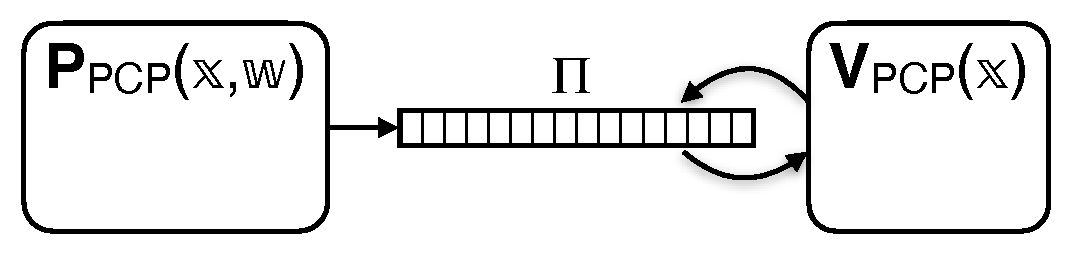
\includegraphics[width=0.55\textwidth]{\FigureFolder/pcp-diagram}
\caption{Diagram of a PCP.}
\label{figure:pcp-diagram}
\end{figure}

The tuple $\PCPSymbol=\PCPSystem$ is a PCP for a relation $\Relation$ with \emph{(perfect) completeness} and \emph{soundness error $\PCPSoundnessError$} if it satisfies the two properties stated below.

\begin{definition}
\label{definition:pcp-completeness}
$\PCPSymbol=\PCPSystem$ for a relation $\Relation$ has \defemph{perfect completeness} if for every $(\Instance,\Witness) \in \Relation$,
\begin{equation*}
\Pr
\left[
\PCPVerifier^{\PCPString}(\Instance)=1
\GivenExperiment
\StateExperiment{
\PCPString \gets \PCPProver(\Instance,\Witness)
}
\right]
=1
\enspace.
\end{equation*}
\end{definition}

In other words, for every true statement, the probability that the (honest) PCP prover produces a PCP string that convinces the (honest) PCP verifier is $1$. The probability is taken over the randomness of the PCP verifier, as well as any randomness used by the PCP prover. (A PCP prover may use randomness, e.g., to achieve zero-knowledge, a property discussed further below.)

\begin{definition}
\label{definition:pcp-soundness}
$\PCPSymbol=\PCPSystem$ for a relation $\Relation$ has \defemph{soundness error $\PCPSoundnessError$} if for every $\Instance \notin \GetLanguage{\Relation}$ and (unbounded) malicious PCP prover $\PCPMaliciousProver$,
\begin{equation*}
\Pr
\left[
\PCPVerifier^{\PCPString}(\Instance)=1
\GivenExperiment
\StateExperiment{
\PCPString \gets \PCPMaliciousProver
}
\right]
\leq
\PCPSoundnessError(\Instance)
\enspace.
\end{equation*}
\end{definition}

In other words, for every false statement, the probability that a computationally unbounded malicious PCP prover outputs a PCP string that convinces the (honest) PCP verifier is at most $\PCPSoundnessError$. The probability is taken over the randomness of the PCP verifier, as well as any randomness of the malicious PCP prover. The malicious PCP prover is computationally unbounded, so randomness does not help (the PCP prover can have the best choice of randomness hardcoded). Nevertheless we provide the more general definition for convenience in later discussions.

The PCP soundness error $\PCPSoundnessError$ depends on the instance $\Instance$ given as input to the PCP verifier. For convenience, we additionally define notation for the largest soundness error across any instance $\Instance$ (not in the language) whose size is at most a bound $\InstanceSize$:
\begin{align*}
\PCPSoundnessError(\InstanceSize)
\DefineEqual
\MaxSoundness{\PCPSoundnessError(\Instance)}
\enspace.
\end{align*}
In particular, we can use $\PCPSoundnessError(\InstanceSize)$ to upper bound the winning probability of a malicious PCP prover that chooses the instance (as long as the instance is not in the language). That is, \Cref{definition:pcp-soundness} implies that for every instance size bound $\InstanceSize \in \Naturals$ and (unbounded) malicious PCP prover $\PCPMaliciousProver$,
\begin{equation*}
\Pr
\left[
\begin{array}{l}
  \SomeSize{\Instance} \leq \InstanceSize \\
  \land\;\Instance \notin \GetLanguage{\Relation} \\
  \land\;\PCPVerifier^{\PCPString}(\Instance)=1
\end{array}
\GivenExperiment
\StateExperiment{
  (\Instance,\PCPString) \gets \PCPMaliciousProver
}
\right]
\leq
\PCPSoundnessError(\InstanceSize)
\enspace.
\end{equation*}

\parhead{Efficiency measures}
We are interested in several efficiency measures of a PCP.
\begin{itemize}

  \item \emph{Alphabet}, denoted $\PCPAlphabet$, is the alphabet used to write the PCP string.

  \item \emph{Proof length}, denoted $\PCPProofLength$, is the number of symbols in the PCP string. The total number of bits in a PCP string is $\PCPProofLength \cdot \log \Cardinality{\PCPAlphabet}$.

  \item \emph{Query complexity}, denoted $\PCPQueryComplexity$, is the number of locations in the PCP string read by the PCP verifier. Each query returns a symbol of $\log \Cardinality{\PCPAlphabet}$ bits.

  \item \emph{Randomness complexity}, denoted $\PCPRandomnessComplexity$, is the number of random bits used by the PCP verifier.

  \item \emph{Prover time and verifier time}, denoted $\PCPProverTime$ and $\PCPVerifierTime$, are the time complexities of the PCP prover (to output the PCP string) and PCP verifier (to output its decision bit), respectively.

\end{itemize}
The above efficiency measures may be functions of the instance $\Instance$ (and possibly other parameters associated to the construction of a PCP).

\parhead{Knowledge soundness}
The soundness notion can be strengthened to a knowledge soundness notion, which informally means that whenever the PCP verifier accepts a PCP string then, up to some error, an efficient deterministic extractor outputs a witness when given the instance and the PCP string. (Note that the extractor does not receive as input the randomness of the PCP verifier.)

\begin{definition}
\label{definition:pcp-knowledge-soundness}
$\PCPSymbol=\PCPSystem$ for a relation $\Relation$ has \defemph{knowledge soundness error $\PCPKnowledgeError$} if there exists a polynomial-time deterministic algorithm $\PCPExtractor$ such that for every instance $\Instance$ and malicious prover $\PCPMaliciousProver$ the following holds:
\begin{equation*}
\Pr\left[
\begin{array}{l}
\PCPVerifier^{\PCPString}(\Instance)=1 \\
\land\;(\Instance,\Witness) \notin \Relation
\end{array}
\GivenExperiment
\StateExperiment{
\PCPString \gets \PCPMaliciousProver \\
\Witness \gets \PCPExtractor(\Instance,\PCPString)
}
\right]
\leq
\PCPKnowledgeError(\Instance)
\enspace.
\end{equation*}
We additionally define $\PCPKnowledgeError(\InstanceSize) \DefineEqual \MaxKnowledge{\PCPKnowledgeError(\Instance)}$.
\end{definition}

If $\PCPSymbol=\PCPSystem$ has knowledge soundness error $\PCPKnowledgeError$ then it has soundness error $\PCPSoundnessError \leq \PCPKnowledgeError$: if $\Instance \notin \GetLanguage{\Relation}$ then the extractor cannot output a witness $\Witness$ such that $(\Instance,\Witness) \in \Relation$, in which case the event bounded by the knowledge soundness condition equals the event bounded by the soundness condition.



\parhead{Zero knowledge}
A notion of zero knowledge for PCPs against honest PCP verifiers suffices for the applications that we study. Informally, zero knowledge states that the \emph{verifier's view} can be efficiently simulated by a probabilistic algorithm that receives as input the instance (but not a corresponding witness). The view consists of the instance, the randomness, and the query answers from the given PCP string. Honest-verifier zero knowledge then requires that the simulated view is statistically close to a view in a real execution, provided that the proved statement is true.

\begin{definition}
\label{definition:pcp-view}
The PCP verifier's \defemph{view} in $\PCPSymbol=\PCPSystem$ on the instance-witness pair $(\Instance,\Witness)$, denoted $\PCPView{\PCPProver}{\PCPVerifier}{\Instance}{\Witness}$, is the random variable $\PCPSampledView$ where:
\begin{itemize}[nolistsep]
  \item $\PCPVerifierRandomMessage \in \Bits^{\PCPRandomnessComplexity}$ is a random choice of randomness for the PCP verifier $\PCPVerifier$;
  \item $\PCPQuerySet \subseteq [\PCPProofLength]$ and $\PCPEntries \in \PCPAlphabet^{\PCPQuerySet}$ are the queries and answers when running $\PCPVerifier^{\PCPString}(\Instance,\PCPVerifierRandomMessage)$ for $\PCPString \gets \PCPProver(\Instance,\Witness)$.
\end{itemize}
The PCP prover $\PCPProver(\Instance,\Witness)$ may use private randomness (not part of the PCP verifier's view).
\end{definition}

\begin{definition}
\label{definition:pcp-hvzk}
$\PCPSymbol=\PCPSystem$ for a relation $\Relation$ has \defemph{honest-verifier zero-knowledge error $\PCPZKError$} if there exists a polynomial-time probabilistic algorithm $\PCPSimulator$ such that for every instance-witness pair $(\Instance,\Witness) \in \Relation$ the following random variables are $\PCPZKError(\Instance)$-close in statistical distance:
\begin{equation*}
\PCPView{\PCPProver}{\PCPVerifier}{\Instance}{\Witness}
\TextAndInMath
\PCPSimulator(\Instance)
\enspace.
\end{equation*}
We additionally define $\PCPZKError(\InstanceSize) \DefineEqual \MaxZK{\PCPZKError(\Instance)}$.
\end{definition}

\parhead{Verification on local views}
We sometimes run a PCP verifier with query access to a \emph{partial} PCP string defined on a subset of locations, and it is useful to introduce notation for this setting.

\begin{definition}
\label{definition:pcp-local-view}
Let $\PCPQuerySet \subseteq [\PCPProofLength]$ be a query set, $\PCPEntries \in \PCPAlphabet^{\PCPQuerySet}$ query answers, $\Instance$ an instance, and $\PCPVerifierRandomMessage \in \Bits^{\PCPRandomnessComplexity}$ a choice of PCP randomness. We denote by
\begin{equation*}
\PCPVerifier^{\PCPLocalView{\PCPQuerySet}{\PCPEntries}}(\Instance,\PCPVerifierRandomMessage)
\end{equation*}
the decision bit of the PCP verifier $\PCPVerifier$, given instance $\Instance$ and PCP randomness $\PCPVerifierRandomMessage$, when each query $\PCPQueryIndex \in \PCPQuerySet$ is answered with $\PCPEntries[\PCPQueryIndex] \in \PCPAlphabet$. (If $\PCPVerifier$ queries outside the set $\PCPQuerySet$ then $\PCPVerifier^{\PCPLocalView{\PCPQuerySet}{\PCPEntries}}(\Instance,\PCPVerifierRandomMessage)=0$.)
\end{definition}

%%%%%%%%%%%%%%%%%%%%%%%%%%%%%%%%%%%%%%%%%%%%%%%%%%%%%%%%%%%%%%%%%%%%%%%%%%%%%%%
%%%%%%%%%%%%%%%%%%%%%%%%%%%%%%%%%%%%%%%%%%%%%%%%%%%%%%%%%%%%%%%%%%%%%%%%%%%%%%%
%%%%%%%%%%%%%%%%%%%%%%%%%%%%%%%%%%%%%%%%%%%%%%%%%%%%%%%%%%%%%%%%%%%%%%%%%%%%%%%
\section{State restoration}
\label{section:pcp-state-restoration}

We introduce the \emph{PCP state restoration game}, where a PCP prover attacks a PCP multiple times. Then we discuss notions of soundness and knowledge soundness associated to this game. These are stronger notions of soundness and knowledge soundness that we use, in later sections, to describe the security properties of the Micali transformation (which we study in \Cref{chapter:micali-transformation}).

These notions are analogous to the notions of state-restoration soundness and knowledge soundness for SPs discussed in \Cref{chapter:fs-for-sp-sr}. Similarly to the case of SPs, good standard soundness implies good state-restoration soundness; specifically, the state-restoration soundness error of a PCP is $\Theta(\ROQueryBound)$ times the standard soundness error of the PCP. Similar considerations hold for state-restoration knowledge soundness compared to standard knowledge soundness.

In this chapter we use state-restoration soundness (and knowledge soundness) as a convenient intermediate step towards the security of the non-interactive argument obtained by applying the Micali transformation to a given PCP, as discussed in \Cref{chapter:micali-transformation}.

\parhead{SR game}
We consider a game where a PCP prover attacks a PCP multiple times. A move consists of proposing an instance $\Instance$ and a PCP string $\PCPString$, and the game responds with a fresh choice of PCP randomness $\PCPVerifierRandomMessage$. The PCP prover can propose the same instance and PCP string more times (to see multiple fresh choices of PCP randomness), but up to some limit (as determined by a salt size). The goal of the PCP prover is to output an instance $\Instance$ and a PCP string $\PCPString$ such that $\PCPVerifier^{\PCPString}(\Instance,\PCPVerifierRandomMessage)=1$ where $\PCPVerifierRandomMessage$ is the PCP randomness chosen for that move. (The PCP prover can also output an instance and PCP string that was not one of its moves.)

We refer to this as a \emph{PCP state-restoration game}, because the adversary is \DoQuote{attacking} the PCP by trying to sample multiple PCP verifier states.

The salt size $\SRSaltSize \in \Naturals$ in the definition below implies that a PCP prover can see at most $2^{\SRSaltSize}$ fresh choices of PCP randomness for the same instance and PCP string. The game's randomness, used to consistently answer the PCP prover's moves, is captured by the random function $\SRRandomness \in \RODistribution{\PCPRandomnessComplexity}$.

\begin{definition}
\label{definition:pcp-state-restoration-game}
The \defemph{PCP state-restoration game} for $\PCPSymbol=\PCPSystem$ with salt size $\SRSaltSize \in \Naturals$, function $\SRRandomness \in \RODistribution{\PCPRandomnessComplexity}$, and PCP state-restoration prover $\PCPMaliciousSRProver$ is defined below.
\begin{itemize}[noitemsep]
\item[] $\PCPStateRestorationGame{\SRSaltSize}{\SRRandomness}{\PCPMaliciousSRProver}$:
\begin{enumerate}[nolistsep]
  \item \label{step:pcp-srgame-main-loop}
  Repeat the following until $\PCPMaliciousSRProver$ decides to exit the loop.
  \begin{enumerate}
    \item \label{step:pcp-srgame-loop-output}
    $\PCPMaliciousSRProver$ outputs $(\Instance,\PCPString,\SRSaltString)$, where $\Instance$ is an instance, $\PCPString \in \PCPAlphabet^{\PCPProofLength}$ is a PCP string, and $\SRSaltString \in \Bits^{\SRSaltSize}$ is a salt string.
    \item Set $\PCPVerifierRandomMessage \DefineEqual \SRRandomness(\Instance,\PCPString,\SRSaltString)$.
    \item Send $\PCPVerifierRandomMessage$ to $\PCPMaliciousSRProver$.
  \end{enumerate}
  \item \label{step:pcp-srgame-final-output} $\PCPMaliciousSRProver$ outputs $(\Instance,\PCPString,\SRSaltString)$, where $\Instance$ is an instance, $\PCPString \in \PCPAlphabet^{\PCPProofLength}$ is a PCP string, and $\SRSaltString \in \Bits^{\SRSaltSize}$ is a salt string.
  \item Set $\PCPVerifierRandomMessage \DefineEqual \SRRandomness(\Instance,\PCPString,\SRSaltString)$.
  \item Output $(\Instance,\PCPString,\SRSaltString,\PCPVerifierRandomMessage)$.
\end{enumerate}
\end{itemize}
We denote by $\SRTrace$ the list of move-response pairs of the form $((\Instance,\PCPString,\SRSaltString),\PCPVerifierRandomMessage)$ performed in the loop. We show $\SRTrace$ in an execution of the PCP state-restoration game using the following notation:
\begin{equation*}
(\Instance,\PCPString,\SRSaltString,\PCPVerifierRandomMessage) \xleftarrow{\SRTrace} \PCPStateRestorationGame{\SRSaltSize}{\SRRandomness}{\PCPMaliciousSRProver}
\enspace.
\end{equation*}
We say that $\PCPMaliciousSRProver$ is \defemph{$\SRBudget$-move} if $\PCPMaliciousSRProver$ exits the loop after at most $\SRBudget$ iterations.
\end{definition}

\parhead{SR soundness}
State-restoration soundness captures the maximum probability that a prover playing the PCP state-restoration game finds an instance and PCP string such that the instance is not in the language and the PCP string convinces the PCP verifier.

\begin{definition}
\label{definition:pcp-state-restoration-soundness}
$\PCPSymbol=\PCPSystem$ has \defemph{state-restoration soundness error $\PCPSRSoundnessError$} if for every salt size $\SRSaltSize \in \Naturals$, move budget $\SRBudget \in \Naturals$, $\SRBudget$-move malicious PCP state-restoration prover $\PCPMaliciousSRProver$, and instance size bound $\InstanceSize \in \Naturals$:
\begin{equation*}
\Pr\left[
\begin{array}{l}
\SomeSize{\Instance} \leq \InstanceSize \\
\land\;\Instance \notin \GetLanguage{\Relation} \\
\land\;\PCPVerifier^{\PCPString}(\Instance,\PCPVerifierRandomMessage)=1
\end{array}
\GivenExperiment
\StateExperiment{
\SRRandomness \gets \RODistribution{\PCPRandomnessComplexity} \\
(\Instance,\PCPString,\SRSaltString,\PCPVerifierRandomMessage) \gets
\PCPStateRestorationGame{\SRSaltSize}{\SRRandomness}{\PCPMaliciousSRProver}
}
\right]
\leq \PCPSRSoundnessError(\SRSaltSize,\SRBudget,\InstanceSize)
\enspace.
\end{equation*}
\end{definition}

The PCP state-restoration game gives the cheating prover $\ROQueryBound+1$ attempts at convincing the PCP verifier (once per loop and once after all loops), each time possibly with a different instance and proof. Intuitively, the maximum winning probability of any cheating prover, for instances not in the language, is at most $\ROQueryBound+1$ times the PCP soundness error. We prove this next.

\begin{theorem}
\label{theorem:pcp-srs-to-soundness}
Let $\PCPSymbol=\PCPSystem$ be a PCP. If $\PCPSymbol$ has soundness error $\PCPSoundnessError$ then $\PCPSymbol$ has state-restoration soundness error $\PCPSRSoundnessError$ such that
\begin{equation*}
\PCPSRSoundnessError(\SRSaltSize,\SRBudget,\InstanceSize)
\leq (\SRBudget+1) \cdot \PCPSoundnessError(\InstanceSize)
\enspace.
\end{equation*}
Note that the salt size $\SRSaltSize$ does not affect the upper bound.

In more detail, there exists a PCP prover $\PCPMaliciousProver$ such that for every salt size $\SRSaltSize \in \Naturals$, move budget $\SRBudget \in \Naturals$, $\SRBudget$-move malicious PCP state-restoration prover $\PCPMaliciousSRProver$, and instance size bound $\InstanceSize \in \Naturals$:
\begin{align*}
& \Pr\left[
\begin{array}{l}
  \SomeSize{\Instance} \leq \InstanceSize \\
  \land\;\Instance \notin \GetLanguage{\Relation} \\
  \land\;\PCPVerifier^{\PCPString}(\Instance,\PCPVerifierRandomMessage)=1
\end{array}
\GivenExperiment
\StateExperiment{
  \SRRandomness \gets \RODistribution{\PCPRandomnessComplexity} \\
  (\Instance,\PCPString,\SRSaltString,\PCPVerifierRandomMessage) \gets
  \PCPStateRestorationGame{\SRSaltSize}{\SRRandomness}{\PCPMaliciousSRProver}
}
\right]
\\ & \leq
(\ROQueryBound+1) \cdot
\Pr \left[
\begin{array}{l}
  \SomeSize{\Instance} \leq \InstanceSize \\
  \land\;\Instance \notin \GetLanguage{\Relation} \\
  \land\;\PCPVerifier^{\PCPString}(\Instance,\PCPVerifierRandomMessage)=1
\end{array}
\GivenExperiment
\StateExperiment{
  (\Instance,\PCPString) \gets \PCPMaliciousProver(\SRSaltSize,\SRBudget,\BlackBox{\PCPMaliciousSRProver}) \\
  \PCPVerifierRandomMessage \gets \Bits^{\PCPRandomnessComplexity}
}
\right]
\enspace.
\end{align*}
\end{theorem}

\begin{construction}
\label{construction-pcp-sr-malicious-prover}
The PCP prover $\PCPMaliciousProver$ receives as input a salt size $\SRSaltSize \in \Naturals$ and move budget $\SRBudget \in \Naturals$ and black-box access to a PCP state-restoration prover $\PCPMaliciousSRProver$, and works as follows.
\begin{enumerate}[noitemsep]
  \item Lazily sample an oracle $\LazySRRandomness \gets \RODistribution{\PCPRandomnessComplexity}$.
  \item Sample a random index $\SRIteration \in [\ROQueryBound+1]$.
  \item Emulate the execution of $\PCPStateRestorationGame{\SRSaltSize}{\LazySRRandomness}{\PCPMaliciousSRProver}$ up to the $\SRIteration$-th output $(\Instance,\PCPString,\SRSaltString)$ of $\PCPMaliciousSRProver$. (There are at most $\ROQueryBound$ outputs in the loop in \Cref{step:pcp-srgame-main-loop}, and an output in \Cref{step:pcp-srgame-final-output}.) Note that black-box access to $\PCPMaliciousSRProver$ suffices for this.
  \item Output $(\Instance,\PCPString)$.
\end{enumerate}
\end{construction}

\begin{proof}
The PCP state-restoration prover $\PCPMaliciousSRProver$ produces at most $\ROQueryBound+1$ outputs: one output per iteration of the loop (there are at most $\ROQueryBound$ iterations), and a final output after the loop. The final output either equals an earlier output or not. We denote by $I$ the set of indices of any appearance of the final output: $I$ contains the index of any iteration in which the final output appears, or (if the final output first appears after the loop) $I$ is a singleton containing the number of iterations plus one. Note that $I$ is a random variable over $\{1,\dots,\ROQueryBound+1\}$ that depends on $\SRRandomness$. Whenever $\SRIteration \in I$, the $\SRIteration$-th output of $\PCPMaliciousSRProver$ equals the final output of $\PCPMaliciousSRProver$, so in this case $\PCPMaliciousProver$ and $\PCPMaliciousSRProver$ output the same instance $\Instance$ and PCP string $\PCPString$. Moreover, the PCP verifier randomness $\PCPVerifierRandomMessage$ is sampled from $\Bits^{\PCPRandomnessComplexity}$, the same distribution as $\PCPVerifierRandomMessage \DefineEqual \SRRandomness(\Instance,\PCPString,\SRSaltString)$ for a random choice of $\SRRandomness \in \RODistribution{\PCPRandomnessComplexity}$. Hence we can write:
\begin{align*}
& \Pr \left[
\begin{array}{l}
  \SomeSize{\Instance} \leq \InstanceSize \\
  \land\;\Instance \notin \GetLanguage{\Relation} \\
  \land\;\PCPVerifier^{\PCPString}(\Instance,\PCPVerifierRandomMessage)=1
\end{array}
\GivenExperiment
\StateExperiment{
  (\Instance,\PCPString) \gets \PCPMaliciousProver(\SRSaltSize,\SRBudget,\BlackBox{\PCPMaliciousSRProver}) \\
  \PCPVerifierRandomMessage \gets \Bits^{\PCPRandomnessComplexity}
}
\right]
\\ & \geq
\Pr \left[
\begin{array}{l}
  \SomeSize{\Instance} \leq \InstanceSize \\
  \land\;\Instance \notin \GetLanguage{\Relation} \\
  \land\;\PCPVerifier^{\PCPString}(\Instance,\PCPVerifierRandomMessage)=1 \\
  \land\;\SRIteration \in I
\end{array}
\GivenExperiment
\StateExperiment{
  \SRRandomness \gets \RODistribution{\PCPRandomnessComplexity} \\
  (\Instance,\PCPString,\SRSaltString,\PCPVerifierRandomMessage) \gets
  \PCPStateRestorationGame{\SRSaltSize}{\SRRandomness}{\PCPMaliciousSRProver} \\
  \SRIteration \gets [\ROQueryBound+1] \\
}
\right]
\enspace.
\end{align*}
Since $\SRIteration$ and $I$ are independent, $\Pr[\SRIteration \in I] \geq \frac{1}{\ROQueryBound+1}$. This lets us lower bound the previous probability:
\begin{equation*}
\geq
\frac{1}{\ROQueryBound+1} \cdot
\Pr \left[
\begin{array}{l}
  \SomeSize{\Instance} \leq \InstanceSize \\
  \land\;\Instance \notin \GetLanguage{\Relation} \\
  \land\;\PCPVerifier^{\PCPString}(\Instance,\PCPVerifierRandomMessage)=1
\end{array}
\GivenExperiment
\StateExperiment{
  \SRRandomness \gets \RODistribution{\PCPRandomnessComplexity} \\
  (\Instance,\PCPString,\SRSaltString,\PCPVerifierRandomMessage) \gets
  \PCPStateRestorationGame{\SRSaltSize}{\SRRandomness}{\PCPMaliciousSRProver}
}
\right]
\enspace.
\end{equation*}
We conclude that:
\begin{align*}
& \Pr \left[
\begin{array}{l}
\SomeSize{\Instance} \leq \InstanceSize \\
\land\;\Instance \notin \GetLanguage{\Relation} \\
\land\;\PCPVerifier^{\PCPString}(\Instance,\PCPVerifierRandomMessage)=1
\end{array}
\GivenExperiment
\StateExperiment{
\SRRandomness \gets \RODistribution{\PCPRandomnessComplexity} \\
(\Instance,\PCPString,\SRSaltString,\PCPVerifierRandomMessage) \gets
\PCPStateRestorationGame{\SRSaltSize}{\SRRandomness}{\PCPMaliciousSRProver}
}
\right]
\\ & \leq
(\ROQueryBound+1) \cdot
\Pr \left[
\begin{array}{l}
  \SomeSize{\Instance} \leq \InstanceSize \\
  \land\;\Instance \notin \GetLanguage{\Relation} \\
  \land\;\PCPVerifier^{\PCPString}(\Instance,\PCPVerifierRandomMessage)=1
\end{array}
\GivenExperiment
\StateExperiment{
  (\Instance,\PCPString) \gets \PCPMaliciousProver(\SRSaltSize,\SRBudget,\BlackBox{\PCPMaliciousSRProver}) \\
  \PCPVerifierRandomMessage \gets \Bits^{\PCPRandomnessComplexity}
}
\right]
\\ & \leq
(\SRBudget +1) \cdot \PCPSoundnessError(\InstanceSize)
\enspace.
\end{align*}
Salts play a meaningful role in the PCP state-restoration game (in that they lead to a more general class of games) but do not affect the above argument.
\end{proof}

\parhead{SR knowledge soundness}
State-restoration knowledge soundness captures the maximum probability that a prover playing the PCP state-restoration game finds an instance and PCP string such that the given extractor cannot find a witness for the instance and the PCP string convinces the PCP verifier.

\begin{definition}
\label{definition:pcp-state-restoration-knowledge-soundness}
$\PCPSymbol=\PCPSystem$ has \defemph{state-restoration knowledge soundness error $\PCPSRKnowledgeError$} if there exists a polynomial-time deterministic algorithm $\PCPSRExtractor$ (the \emph{extractor}) such that for every salt size $\SRSaltSize \in \Naturals$, move budget $\SRBudget \in \Naturals$, $\SRBudget$-move deterministic PCP state-restoration prover $\PCPMaliciousSRProver$, and instance size bound $\InstanceSize$:
\begin{equation*}
\Pr\left[
\begin{array}{l}
\SomeSize{\Instance} \leq \InstanceSize \\
\land\;(\Instance,\Witness) \notin \Relation \\
\land\;\PCPVerifier^{\PCPString}(\Instance,\PCPVerifierRandomMessage)=1
\end{array}
\GivenExperiment
\StateExperiment{
\SRRandomness \gets \RODistribution{\PCPRandomnessComplexity} \\
(\Instance,\PCPString,\SRSaltString,\PCPVerifierRandomMessage) \gets
\PCPStateRestorationGame{\SRSaltSize}{\SRRandomness}{\PCPMaliciousSRProver} \\
\Witness \gets \PCPSRExtractor(\Instance,\PCPString)
}
\right]
\leq \PCPSRKnowledgeError(\SRSaltSize,\SRBudget,\InstanceSize)
\enspace.
\end{equation*}
\end{definition}

Similarly to \Cref{theorem:pcp-srs-to-soundness}, $(\ROQueryBound+1)$ times the knowledge soundness error of a PCP is an upper bound on its state-restoration knowledge soundness error.

\begin{theorem}
\label{theorem:pcp-srk-to-knowledge}
Let $\PCPSymbol=\PCPSystem$ be a PCP. If $\PCPSymbol$ has knowledge soundness error $\PCPKnowledgeError$ then $\PCPSymbol$ has state-restoration knowledge soundness error $\PCPSRKnowledgeError$ such that
\begin{equation*}
\PCPSRKnowledgeError(\SRSaltSize,\SRBudget,\InstanceSize)
\leq (\SRBudget +1) \cdot \PCPKnowledgeError(\InstanceSize)
\enspace.
\end{equation*}
Note that the salt size $\SRSaltSize$ does not affect the upper bound.

In more detail, letting $\PCPExtractor$ be the knowledge extractor for $\PCPSymbol$, there exists a PCP prover $\PCPMaliciousProver$ and a PCP state-restoration extractor $\PCPSRExtractor$ such that for every salt size $\SRSaltSize \in \Naturals$, move budget $\SRBudget \in \Naturals$, $\SRBudget$-move malicious PCP state-restoration prover $\PCPMaliciousSRProver$, and instance size bound $\InstanceSize \in \Naturals$:
\begin{align*}
& \Pr\left[
\begin{array}{l}
  \SomeSize{\Instance} \leq \InstanceSize \\
  \land\;(\Instance,\Witness) \notin \Relation \\
  \land\;\PCPVerifier^{\PCPString}(\Instance,\PCPVerifierRandomMessage)=1
\end{array}
\GivenExperiment
\StateExperiment{
  \SRRandomness \gets \RODistribution{\PCPRandomnessComplexity} \\
(\Instance,\PCPString,\SRSaltString,\PCPVerifierRandomMessage) \gets
\PCPStateRestorationGame{\SRSaltSize}{\SRRandomness}{\PCPMaliciousSRProver} \\
\Witness \gets \PCPSRExtractor(\Instance,\PCPString)
}
\right]
\\ & \leq
(\ROQueryBound+1) \cdot
\Pr \left[
\begin{array}{l}
  \SomeSize{\Instance} \leq \InstanceSize \\
  \land\;(\Instance, \Witness) \notin \Relation \\
  \land\;\PCPVerifier^{\PCPString}(\Instance,\PCPVerifierRandomMessage)=1
\end{array}
\GivenExperiment
\StateExperiment{
  (\Instance,\PCPString) \gets \PCPMaliciousProver(\SRSaltSize,\SRBudget,\BlackBox{\PCPMaliciousSRProver}) \\
  \PCPVerifierRandomMessage \gets \Bits^{\PCPRandomnessComplexity} \\
  \Witness \gets \PCPExtractor(\Instance,\PCPString)
}
\right]
\enspace.
\end{align*}
\end{theorem}

\begin{proof}
The proof is similar to the soundness proof in \Cref{theorem:pcp-srs-to-soundness}. Let $\PCPMaliciousProver$ be the PCP prover in \Cref{construction-pcp-sr-malicious-prover}. The extractor $\PCPSRExtractor$ applies the extractor $\PCPExtractor$ of the underlying PCP: $\PCPSRExtractor(\Instance,\PCPString) \DefineEqual \PCPExtractor(\Instance,\PCPString)$. We are left to argue the success probability of this extractor.

The PCP state-restoration prover $\PCPMaliciousSRProver$ produces at most $\ROQueryBound+1$ outputs: one output per iteration of the loop (there are at most $\ROQueryBound$ iterations), and a final output after the loop. The final output either equals an earlier output or not. We denote by $I$ the set of indices of any appearance of the final output: $I$ contains the index of any iteration in which the final output appears, or (if the final output first appears after the loop) $I$ is a singleton containing the number of iterations plus one. Note that $I$ is a random variable over $\{1,\dots,\ROQueryBound+1\}$ that depends on $\SRRandomness$. Whenever $\SRIteration \in I$, the $\SRIteration$-th output of $\PCPMaliciousSRProver$ equals the final output of $\PCPMaliciousSRProver$, so in this case $\PCPMaliciousProver$ and $\PCPMaliciousSRProver$ output the same instance $\Instance$ and PCP string $\PCPString$. Moreover, the PCP verifier randomness $\PCPVerifierRandomMessage$ is sampled from $\Bits^{\PCPRandomnessComplexity}$, the same distribution as $\PCPVerifierRandomMessage \DefineEqual \SRRandomness(\Instance,\PCPString,\SRSaltString)$ for a random choice of $\SRRandomness \in \RODistribution{\PCPRandomnessComplexity}$. Hence we can write:
\begin{align*}
& \Pr \left[
\begin{array}{l}
  \SomeSize{\Instance} \leq \InstanceSize \\
  \land\;(\Instance,\Witness) \notin \Relation \\
  \land\;\PCPVerifier^{\PCPString}(\Instance,\PCPVerifierRandomMessage)=1
\end{array}
\GivenExperiment
\StateExperiment{
  (\Instance,\PCPString) \gets \PCPMaliciousProver(\SRSaltSize,\SRBudget,\BlackBox{\PCPMaliciousSRProver}) \\
  \PCPVerifierRandomMessage \gets \Bits^{\PCPRandomnessComplexity} \\
  \Witness \gets \PCPExtractor(\Instance,\PCPString)
}
\right]
\\ & \geq
\Pr \left[
\begin{array}{l}
  \SomeSize{\Instance} \leq \InstanceSize \\
  \land\;(\Instance,\Witness) \notin \Relation \\
  \land\;\PCPVerifier^{\PCPString}(\Instance,\PCPVerifierRandomMessage)=1 \\
  \land\;\SRIteration \in I
\end{array}
\GivenExperiment
\StateExperiment{
  \SRRandomness \gets \RODistribution{\PCPRandomnessComplexity} \\
  (\Instance,\PCPString,\SRSaltString,\PCPVerifierRandomMessage) \gets
  \PCPStateRestorationGame{\SRSaltSize}{\SRRandomness}{\PCPMaliciousSRProver} \\
  \Witness \gets \PCPSRExtractor(\Instance,\PCPString) \\
   \SRIteration \gets [\ROQueryBound+1] \\
}
\right]
\enspace.
\end{align*}
Since $\SRIteration$ and $I$ are independent, $\Pr[\SRIteration \in I] \geq \frac{1}{\ROQueryBound+1}$. This lets us lower bound the previous probability:
\begin{equation*}
\geq
\frac{1}{\ROQueryBound+1} \cdot
\Pr \left[
\begin{array}{l}
  \SomeSize{\Instance} \leq \InstanceSize \\
  \land\;(\Instance,\Witness) \notin \Relation \\
  \land\;\PCPVerifier^{\PCPString}(\Instance,\PCPVerifierRandomMessage)=1
\end{array}
\GivenExperiment
\StateExperiment{
  \SRRandomness \gets \RODistribution{\PCPRandomnessComplexity} \\
  (\Instance,\PCPString,\SRSaltString,\PCPVerifierRandomMessage) \gets
  \PCPStateRestorationGame{\SRSaltSize}{\SRRandomness}{\PCPMaliciousSRProver} \\
  \Witness \gets \PCPSRExtractor(\Instance,\PCPString)
}
\right]
\enspace.
\end{equation*}
We conclude that:
\begin{align*}
& \Pr \left[
\begin{array}{l}
  \SomeSize{\Instance} \leq \InstanceSize \\
  \land\;(\Instance,\Witness) \notin \Relation \\
  \land\;\PCPVerifier^{\PCPString}(\Instance,\PCPVerifierRandomMessage)=1
\end{array}
\GivenExperiment
\StateExperiment{
  \SRRandomness \gets \RODistribution{\PCPRandomnessComplexity} \\
  (\Instance,\PCPString,\SRSaltString,\PCPVerifierRandomMessage) \gets
  \PCPStateRestorationGame{\SRSaltSize}{\SRRandomness}{\PCPMaliciousSRProver} \\
  \Witness \gets \PCPSRExtractor(\Instance,\PCPString)
}
\right]
\\ & \leq
(\ROQueryBound+1) \cdot
\Pr \left[
\begin{array}{l}
  \SomeSize{\Instance} \leq \InstanceSize \\
  \land\;(\Instance, \Witness) \notin \Relation \\
  \land\;\PCPVerifier^{\PCPString}(\Instance,\PCPVerifierRandomMessage)=1
\end{array}
\GivenExperiment
\StateExperiment{
  (\Instance,\PCPString) \gets \PCPMaliciousProver(\SRSaltSize,\SRBudget,\BlackBox{\PCPMaliciousSRProver}) \\
  \PCPVerifierRandomMessage \gets \Bits^{\PCPRandomnessComplexity} \\
  \Witness \gets \PCPExtractor(\Instance,\PCPString)
}
\right]
\\ & \leq
(\SRBudget +1) \cdot \PCPKnowledgeError(\InstanceSize)
\enspace.
\end{align*}
\end{proof}

%%%%%%%%%%%%%%%%%%%%%%%%%%%%%%%%%%%%%%%%%%%%%%%%%%%%%%%%%%%%%%%%%%%%%%%%%%%%%%%
%%%%%%%%%%%%%%%%%%%%%%%%%%%%%%%%%%%%%%%%%%%%%%%%%%%%%%%%%%%%%%%%%%%%%%%%%%%%%%%
%%%%%%%%%%%%%%%%%%%%%%%%%%%%%%%%%%%%%%%%%%%%%%%%%%%%%%%%%%%%%%%%%%%%%%%%%%%%%%%
%%%%%%%%%%%%%%%%%%%%%%%%%%%%%%%%%%%%%%%%%%%%%%%%%%%%%%%%%%%%%%%%%%%%%%%%%%%%%%%
\chapter{Warmup: succinct interactive arguments from PCPs}
\label{chapter:kilian-transformation}

We describe how to construct a succinct \emph{interactive} argument, starting from any probabilistically checkable proof (PCP). This is known as the \emph{Kilian transformation} \cite{Kilian92}. Later, in \Cref{chapter:micali-transformation}, we build on this to construct a succinct \emph{non-interactive} argument (again starting from any PCP). Throughout, we assume familiarity with the Merkle commitment scheme (which we study in \Cref{chapter:merkle-commitment}).

%%%%%%%%%%%%%%%%%%%%%%%%%%%%%%%%%%%%%%%%%%%%%%%%%%%%%%%%%%%%%%%%%%%%%%%%%%%%%%%
%%%%%%%%%%%%%%%%%%%%%%%%%%%%%%%%%%%%%%%%%%%%%%%%%%%%%%%%%%%%%%%%%%%%%%%%%%%%%%%
%%%%%%%%%%%%%%%%%%%%%%%%%%%%%%%%%%%%%%%%%%%%%%%%%%%%%%%%%%%%%%%%%%%%%%%%%%%%%%%
\section{Construction}
\label{section:kilian-construction}

The PCP model envisages a setting where the PCP verifier has query access to a proof string. The succinct interactive argument that we describe here relies on the Merkle commitment scheme to \DoQuote{implement} this query access interface, as we now elaborate.

The argument verifier wishes to query the PCP string but can neither receive it (the PCP string is too long) nor trust the argument prover to answer queries (the argument prover could choose how to answer based on the received queries). The Kilian transformation resolves this via a commit-challenge-response structure that is a common paradigm in cryptographic protocols (e.g., many SPs follow this structure); in particular, the transformation relies on the Merkle commitment scheme, which provides succinct commitments with local openings (in the random oracle model).
\begin{enumerate}[noitemsep]

  \item \emph{Commit} ($\ARGProver \to \ARGVerifier$).
  The argument prover sends to the argument verifier a short Merkle commitment to the PCP string.

  \item \emph{Challenge} ($\ARGVerifier \to \ARGProver$).
  The argument verifier sends PCP randomness to the argument prover, which determines a set of queries.

  \item \emph{Response} ($\ARGProver \to \ARGVerifier$).
  The argument prover opens the queried locations of the PCP string.

\end{enumerate}
The first message ensures that the argument prover is (computationally) bound to a particular PCP string via the Merkle commitment, and so the argument verifier does not have to worry about sending the PCP randomness to the argument prover in the second message. The third (and final) message authenticates the claimed answers relative to the Merkle commitment. This sketch is merely an intuition, and we will see that establishing a formal security proof requires some work.

Below we describe the construction in detail.

\begin{ImportantConstruction}{\KilianText}{kilian-transformation}
Let $\PCPSymbol=\PCPSystem$ be a PCP with proof length $\PCPProofLength$ over alphabet $\PCPAlphabet$, query complexity $\PCPQueryComplexity$, and randomness complexity $\PCPRandomnessComplexity$. Let $\SecurityParameter \in \Naturals$ be a security parameter and $\PrivacyParameter \in \Naturals$ be a privacy parameter. Define $\MTSymbol \DefineEqual \MTConstructor{\SecurityParameter}{\PCPAlphabet}{\PCPProofLength}{\PrivacyParameter}$ to be the Merkle commitment scheme with the stated parameters. (The output size of the random oracle for the Merkle commitment scheme equals the security parameter $\SecurityParameter$.)

We define $\IARGSymbol \DefineEqual \KilianTransformation{\PCPSymbol}{\SecurityParameter}{\PrivacyParameter}$ to be the $3$-message public-coin interactive argument $\IARGSymbol = \ARGSystem$ constructed as follows. The argument prover $\ARGProver$ receives as input an instance $\Instance$ and witness $\Witness$, and the argument verifier $\ARGVerifier$ receives as input the instance $\Instance$. Both receive query access to a random oracle $\ROFunction \in \RODistribution{\SecurityParameter}$ and they interact as below.
\begin{enumerate}

\item \emph{Commit.}
The argument prover $\ARGProver$ computes its first message as follows.
\begin{enumerate}[nolistsep]
  \item Compute the PCP string $\PCPString \DefineEqual \PCPProver(\Instance,\Witness) \in \PCPAlphabet^{\PCPProofLength}$.
  \item Commit to $\PCPString$ via the Merkle commitment scheme: $(\MTCommitment,\MTTrapdoor) \DefineEqual \MTCommit^{\ROFunction}(\PCPString)$.
  \item Send the Merkle commitment $\MTCommitment \in \Bits^{\SecurityParameter}$.
\end{enumerate}

\item \emph{Challenge.}
The argument verifier $\ARGVerifier$ sends randomness $\PCPVerifierRandomMessage \in \Bits^{\PCPRandomnessComplexity}$ for the PCP verifier $\PCPVerifier$.

\item \emph{Response.}
The argument prover $\ARGProver$ computes its second message as follows.
\begin{enumerate}[nolistsep]
  \item Simulate the PCP verifier $\PCPVerifier^{\PCPString}(\Instance,\PCPVerifierRandomMessage)$, yielding a query set $\PCPQuerySet \subseteq [\PCPProofLength]$ with $\Cardinality{\PCPQuerySet} \leq \PCPQueryComplexity$.
  \item Set $\PCPEntries \DefineEqual \PCPString[\PCPQuerySet] \in \PCPAlphabet^{\PCPQuerySet}$ to be the answers for the query set.
  \item Compute an opening proof for $\PCPEntries$: $\MTProof \DefineEqual \MTOpen^{\ROFunction}(\MTTrapdoor, \PCPQuerySet)$.
  \item Send $(\PCPQuerySet,\PCPEntries,\MTProof)$.
\end{enumerate}

\item \emph{Verification.}
The argument verifier $\ARGVerifier$ checks the following.
\begin{enumerate}[nolistsep]
  \item Check that $\PCPVerifier^{\PCPLocalView{\PCPQuerySet}{\PCPEntries}}(\Instance,\PCPVerifierRandomMessage)=1$. (The PCP verifier $\PCPVerifier(\Instance,\PCPVerifierRandomMessage)$ accepts if each query $\PCPQueryIndex \in \PCPQuerySet$ is answered with $\PCPEntries[\PCPQueryIndex] \in \PCPAlphabet$. If any query falls outside the set $\PCPQuerySet$ then reject.)
  \item Check that $\MTCheck^{\ROFunction}(\MTCommitment,\PCPQuerySet,\PCPEntries,\MTProof)=1$. (The query answers $\PCPEntries \in \PCPAlphabet^{\PCPQuerySet}$ are authenticated with respect to the Merkle commitment $\MTCommitment$.)
\end{enumerate}

\end{enumerate}
\end{ImportantConstruction}

\parhead{Efficiency}
We discuss efficiency properties of the above construction.
\begin{itemize}

  \item \emph{Communication complexity.}
  The argument prover sends to the argument verifier:
  \begin{itemize}[nolistsep]
    \item one Merkle commitment $\MTCommitment$, consisting of $\SecurityParameter$ bits;
    \item $\PCPQueryComplexity$ query-answer pairs, consisting of $\PCPQueryComplexity \cdot (\log \PCPProofLength + \log \Cardinality{\PCPAlphabet})$ bits; and
    \item a Merkle opening proof for $\PCPQueryComplexity$ locations, consisting of at most $\PCPQueryComplexity \cdot (\PrivacyParameter + \SecurityParameter \cdot \log \PCPProofLength)$ bits.\footnote{See \Cref{section:compressing-opening-proof} for more on the size of Merkle opening proofs.}
  \end{itemize}
Hence the number of bits sent by the argument prover is at most:
\begin{equation}
\label{equation:kilian-prover-to-verifier}
\SecurityParameter
+
\PCPQueryComplexity
\cdot
(
  \log \PCPProofLength
+ \log \Cardinality{\PCPAlphabet}
+ \PrivacyParameter
+ \SecurityParameter \cdot \log \PCPProofLength
)
= O\big(
\PCPQueryComplexity
\cdot
(\log \Cardinality{\PCPAlphabet} + \PrivacyParameter + \SecurityParameter \cdot \log \PCPProofLength)
\big)
\enspace.
\end{equation}
In the other direction, the argument verifier sends to the argument prover the randomness $\PCPVerifierRandomMessage$, which consists of $\PCPRandomnessComplexity$ bits. If zero knowledge is not a goal, the privacy parameter $\PrivacyParameter$ equals $0$.

Simply sending the (uncommitted) PCP string $\PCPString$ would have cost $\PCPProofLength \cdot \log \Cardinality{\PCPAlphabet}$ bits. Therefore, using the Merkle commitment scheme to succinctly commit to the PCP string and then locally open the queried locations reduces the communication complexity to $\PCPQueryComplexity \cdot (\log \PCPProofLength + \log \Cardinality{\PCPAlphabet})$ plus the information that is used to commit and authenticate. For most parameter settings, this is significantly smaller than the number of bits in the PCP string, achieving the desired \DoQuote{succinct communication complexity}.

  \item \emph{Prover complexity.}
  The complexity of the argument prover is typically dominated by the complexity of the underlying PCP prover. Moreover, the number of queries to the random oracle is $\ARGQueryP = O(\PCPProofLength)$ (to commit to the PCP string).

  \item \emph{Verifier complexity.}
  The complexity of the argument verifier is typically dominated by the complexity of the underlying PCP verifier. Moreover, the number of queries to the random oracle is $\ARGQueryV = O(\PCPQueryComplexity \cdot \log \PCPProofLength)$ (to check the Merkle opening proof for $\PCPQueryComplexity$ answers).

\end{itemize}

\begin{figure}[htp!]
\centering
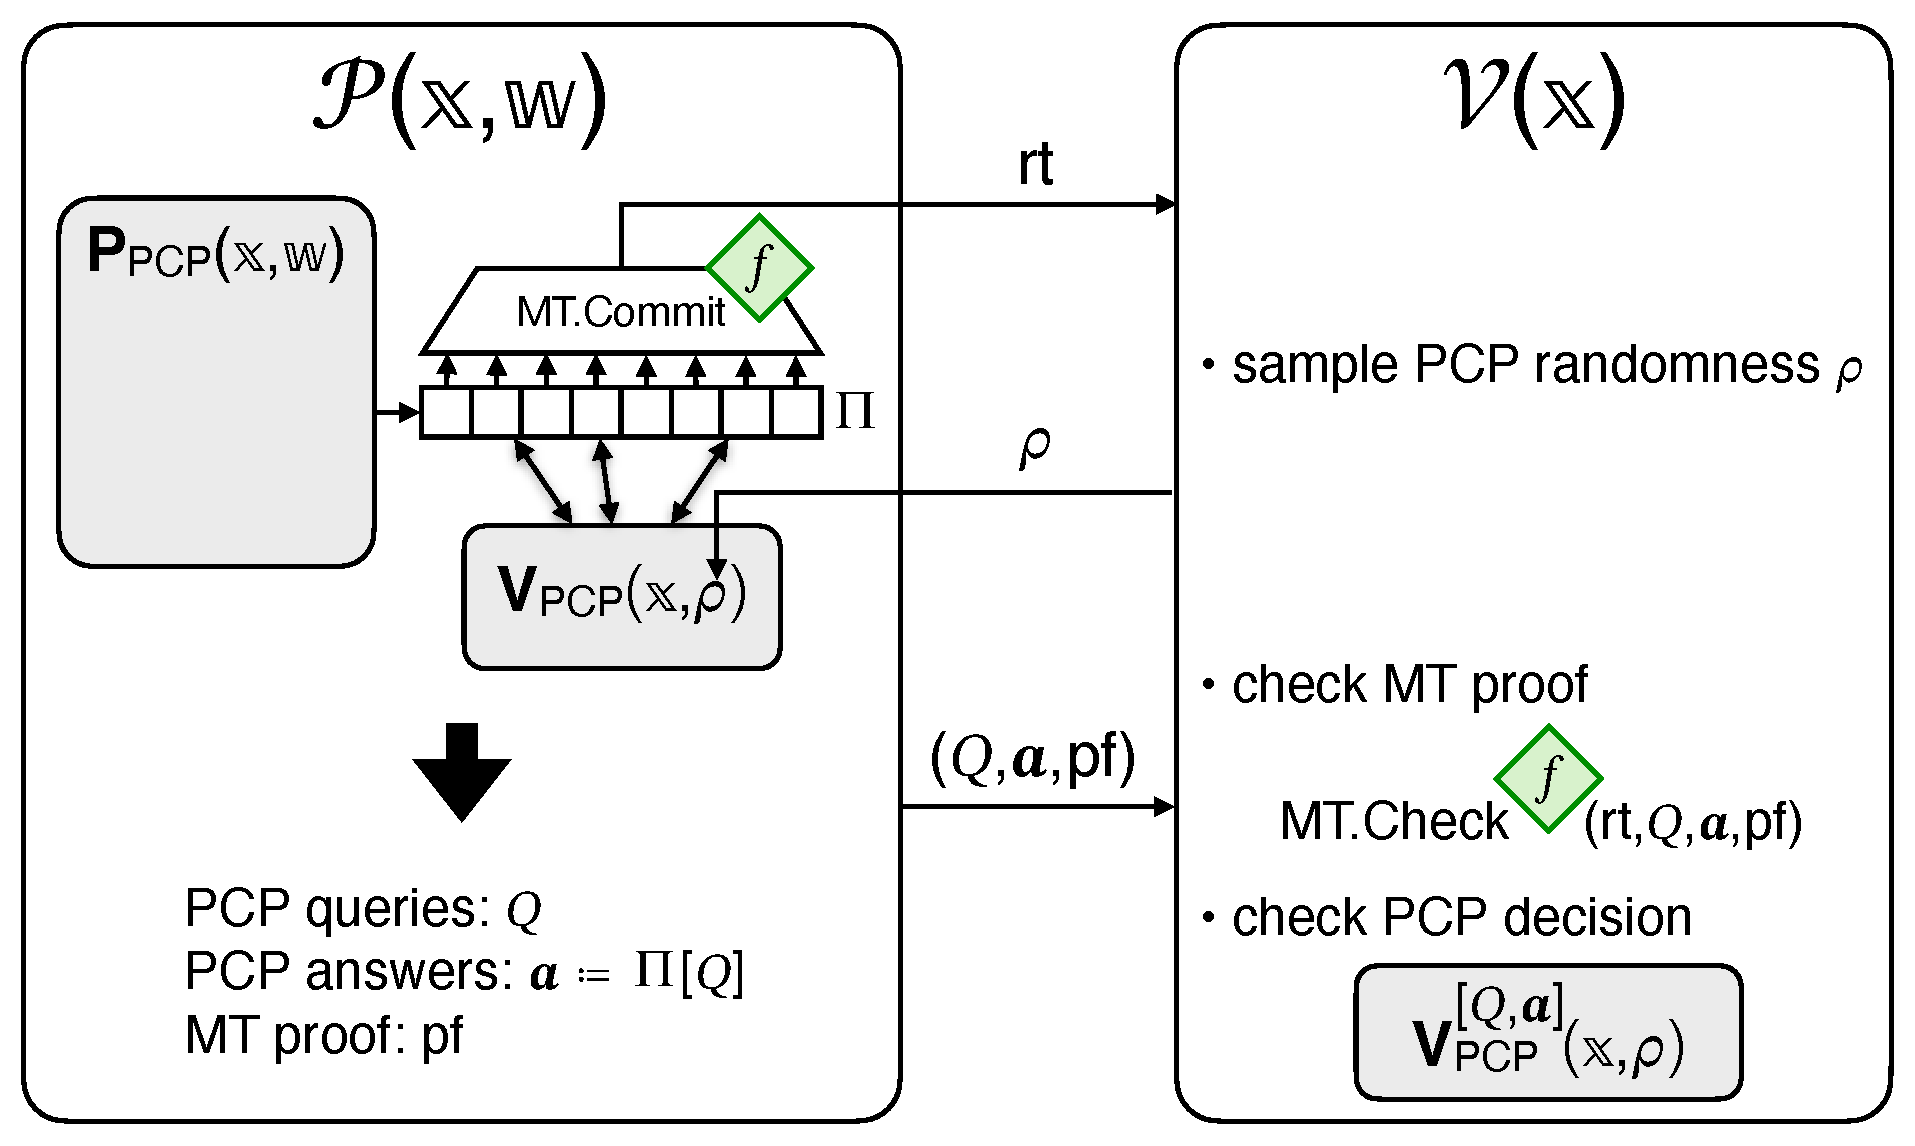
\includegraphics[width=0.8\textwidth]{\FigureFolder/kilian-diagram}
\caption[Diagram of the Kilian transformation]{Diagram of the \KilianText ($\KilianSymbol$ in \Cref{construction:kilian-transformation}).}
\label{figure:kilian-diagram}
\end{figure}

%%%%%%%%%%%%%%%%%%%%%%%%%%%%%%%%%%%%%%%%%%%%%%%%%%%%%%%%%%%%%%%%%%%%%%%%%%%%%%%
%%%%%%%%%%%%%%%%%%%%%%%%%%%%%%%%%%%%%%%%%%%%%%%%%%%%%%%%%%%%%%%%%%%%%%%%%%%%%%%
%%%%%%%%%%%%%%%%%%%%%%%%%%%%%%%%%%%%%%%%%%%%%%%%%%%%%%%%%%%%%%%%%%%%%%%%%%%%%%%
\section{Non-adaptive soundness}
\label{section:kilian-nonadaptive-soundness}

We prove that \Cref{construction:kilian-transformation} is \emph{non-adaptively} sound (\Cref{definition:iarg-nonadaptive-soundness}): for every instance that is not in the language, the probability that a bounded-query adversary convinces the argument verifier is small. \Cref{theorem:kilian-nonadaptive-soundness} below provides an upper bound on this error, which is the soundness error of the underlying PCP plus a small term. This term represents the error incurred by \DoQuote{breaking} (the extractability property of) the Merkle commitment scheme used to commit to the PCP string. Later in \Cref{section:kilian-adaptive-soundness} we prove that \Cref{construction:kilian-transformation} is also \emph{adaptively} sound.

\begin{ImportantTheorem}{}{kilian-nonadaptive-soundness}
Let $\PCPSymbol$ be a PCP for a relation $\Relation$ with soundness error $\PCPSoundnessError$ and proof length $\PCPProofLength$. For every security parameter $\SecurityParameter \in \Naturals$ and privacy parameter $\PrivacyParameter \in \Naturals$, $\IARGSymbol \DefineEqual \KilianTransformation{\PCPSymbol}{\SecurityParameter}{\PrivacyParameter}$ in \Cref{construction:kilian-transformation} is an interactive argument for $\Relation$ with non-adaptive soundness error $\ARGNASoundnessError$ (see \Cref{definition:iarg-nonadaptive-soundness}) such that
\begin{equation*}
\ARGNASoundnessError(\SecurityParameter,\ROQueryBound,\Instance)
\leq
\PCPSoundnessError(\Instance)
+
\MTExtractionError(\SecurityParameter,\ROQueryBound,\PCPProofLength)
\enspace.
\end{equation*}
Above $\MTExtractionError$ is the Merkle commitment extraction error from \Cref{lemma:mt-extractability}, and $\MTExtractionError(\SecurityParameter,\ROQueryBound,\PCPProofLength) \leq \MTExtractabilityShortExpression{\SecurityParameter}{\ROQueryBound}$ if $\MTExtractabilityCondition{\ROQueryBound}{\PCPProofLength}{\log\PCPProofLength}$.
\end{ImportantTheorem}

We prove the theorem via a security reduction of the following form. For every fixed instance $\Instance$, any malicious argument prover $\Malicious{\ARGProver}$ that convinces the argument verifier $\ARGVerifier(\Instance)$ with probability $\delta$ can be transformed into a corresponding malicious PCP prover $\PCPMaliciousProver$ that convinces the PCP verifier $\PCPVerifier(\Instance)$ with probability at least $\delta$ minus a small term. \Cref{theorem:kilian-nonadaptive-soundness} follows by noting that if $\Instance \notin \GetLanguage{\Relation}$ then the PCP verifier accepts $\Instance$ with probability at most $\PCPSoundnessError(\Instance)$.

Below we state the security reduction and then prove it.

\begin{lemma}
\label{lemma:kilian-nonadaptive-reduction}
There exists a PCP prover $\PCPMaliciousProver$ such that for every $\ROQueryBound$-query argument prover $\Malicious{\ARGProver}$ the following holds for every instance $\Instance$:
\begin{equation*}
\Pr
\left[
\ARGInteract{\Malicious{\ARGProver}^{\ROFunction}}{\ARGVerifier^{\ROFunction}(\Instance)}=1
\GivenExperiment
\StateExperiment{
\ROFunction \gets \RODistribution{\SecurityParameter}
}
\right]
\leq
\Pr
\left[
\PCPVerifier^{\PCPString}(\Instance,\PCPVerifierRandomMessage)=1
\GivenExperiment
\StateExperiment{
\PCPString \gets \PCPMaliciousProver(\BlackBox{\ARGProver}) \\
\PCPVerifierRandomMessage \gets \Bits^{\PCPRandomnessComplexity}
}
\right]
+
\MTExtractionError(\SecurityParameter,\ROQueryBound,\PCPProofLength)
\enspace.
\end{equation*}
Moreover, the running time of $\PCPMaliciousProver$ equals the running time of $\Malicious{\ARGProver}$ plus $\MTExtractorTimeFunction{\SecurityParameter}{\PCPAlphabet}{\PCPProofLength}{\PrivacyParameter}{\ROQueryBound}$ where $\MTExtractorTimeSymbol$ is the time complexity of the Merkle commitment extractor in \Cref{lemma:mt-extractability}.
\end{lemma}

\begin{proof}
Let $\MTExtractor$ be the Merkle commitmnet extractor from \Cref{lemma:mt-extractability} in \Cref{section:merkle-commitment-single-extractability}. The PCP prover $\PCPMaliciousProver$ works as follows.
\begin{itemize}
\item[] $\PCPMaliciousProver(\BlackBox{\ARGProver})$:
\begin{enumerate}[nolistsep]

  \item Run the argument prover $\Malicious{\ARGProver}$, simulating its random oracle $\ROFunction$, until $\Malicious{\ARGProver}$ outputs a Merkle commitment $\MTCommitment$; let $\ROTrace$ be the query-answer trace of this partial execution. (The argument prover $\Malicious{\ARGProver}$ is an interactive algorithm, whose full execution would also involve giving PCP randomness $\PCPVerifierRandomMessage$ to $\Malicious{\ARGProver}$ and then obtaining the next message of $\Malicious{\ARGProver}$. Here we use a partial execution.)

  \item Run the Merkle commitment extractor to obtain a PCP string:
  \begin{equation*}
  (\PCPString,\MTTrapdoor) \gets \MTExtractor(\MTCommitment,\ROTrace)
  \enspace.
  \end{equation*}
  ($\MTExtractor$ also outputs an opening trapdoor $\MTTrapdoor$, but it is not used here.)

  \item Output the PCP string $\PCPString$.

\end{enumerate}
\end{itemize}
The PCP prover $\PCPMaliciousProver$ uses the argument prover $\Malicious{\ARGProver}$ as a black box. The running time of $\PCPMaliciousProver$ is the running time of (a partial execution of) $\Malicious{\ARGProver}$ plus the running time of the (efficient) extractor $\MTExtractor$ on a query-answer trace of size at most $\ROQueryBound$.

We argue that the PCP prover $\PCPMaliciousProver$ satisfies the claimed property.

By construction, the argument verifier $\ARGVerifier$ accepts if and only if the PCP verifier $\PCPVerifier$ accepts and the Merkle commitment checking algorithm $\MTCheck$ accepts:
\begin{align*}
&\Pr
\left[
\ARGInteract{\Malicious{\ARGProver}^{\ROFunction}}{\ARGVerifier^{\ROFunction}(\Instance)}=1
\GivenExperiment
\StateExperiment{
\ROFunction \gets \RODistribution{\SecurityParameter}
}
\right]
\\
=&
\Pr
\left[
\begin{array}{l}
\PCPVerifier^{\PCPLocalView{\PCPQuerySet}{\PCPEntries}}(\Instance,\PCPVerifierRandomMessage)=1 \\
\land\;\MTCheck^{\ROFunction}(\MTCommitment,\PCPQuerySet,\PCPEntries,\MTProof)=1
\end{array}
\GivenExperiment
\StateExperiment{
\ROFunction \gets \RODistribution{\SecurityParameter} \\
(\MTCommitment,\ROAdvState) \gets \Malicious{\ARGProver}^{\ROFunction} \\
\PCPVerifierRandomMessage \gets \Bits^{\PCPRandomnessComplexity} \\
(\PCPQuerySet,\PCPEntries,\MTProof) \gets \Malicious{\ARGProver}^{\ROFunction}(\ROAdvState,\PCPVerifierRandomMessage)
}
\right]
\enspace.
\end{align*}
We split the above probability as a sum of two probabilities that separately consider the disjoint cases $\PCPString[\PCPQuerySet] = \PCPEntries$ and $\PCPString[\PCPQuerySet] \neq \PCPEntries$ where $\PCPString$ is the PCP string output by $\MTExtractor$:
\begin{align}
\label{equation:kilian-nonadaptive-soundess-ext-works}
&\Pr
\left[
\begin{array}{l}
\PCPVerifier^{\PCPLocalView{\PCPQuerySet}{\PCPEntries}}(\Instance,\PCPVerifierRandomMessage)=1 \\
\land\;\MTCheck^{\ROFunction}(\MTCommitment,\PCPQuerySet,\PCPEntries,\MTProof)=1 \\
\land\;\PCPString[\PCPQuerySet] = \PCPEntries
\end{array}
\GivenExperiment
\StateExperiment{
\ROFunction \gets \RODistribution{\SecurityParameter} \\
\ROOutputAndTrace{\ROFunction}{\Malicious{\ARGProver}}{\ROTrace}{(\MTCommitment,\ROAdvState)} \\
(\PCPString,\MTTrapdoor) \gets \MTExtractor(\MTCommitment,\ROTrace) \\
\PCPVerifierRandomMessage \gets \Bits^{\PCPRandomnessComplexity} \\
(\PCPQuerySet,\PCPEntries,\MTProof) \gets \Malicious{\ARGProver}^{\ROFunction}(\ROAdvState,\PCPVerifierRandomMessage)
}
\right] \\
\label{equation:kilian-nonadaptive-soundess-ext-fails}
+&
\Pr
\left[
\begin{array}{l}
\PCPVerifier^{\PCPLocalView{\PCPQuerySet}{\PCPEntries}}(\Instance,\PCPVerifierRandomMessage)=1 \\
\land\;\MTCheck^{\ROFunction}(\MTCommitment,\PCPQuerySet,\PCPEntries,\MTProof)=1 \\
\land\;\PCPString[\PCPQuerySet] \neq \PCPEntries
\end{array}
\GivenExperiment
\StateExperiment{
\ROFunction \gets \RODistribution{\SecurityParameter} \\
\ROOutputAndTrace{\ROFunction}{\Malicious{\ARGProver}}{\ROTrace}{(\MTCommitment,\ROAdvState)} \\
(\PCPString,\MTTrapdoor) \gets \MTExtractor(\MTCommitment,\ROTrace) \\
\PCPVerifierRandomMessage \gets \Bits^{\PCPRandomnessComplexity} \\
(\PCPQuerySet,\PCPEntries,\MTProof) \gets \Malicious{\ARGProver}^{\ROFunction}(\ROAdvState,\PCPVerifierRandomMessage)
}
\right]
\enspace.
\end{align}
We conclude the proof by upper bounding each of the two terms.
\begin{itemize}

  \item The term in \Cref{equation:kilian-nonadaptive-soundess-ext-works} is upper bounded by the PCP error, as we now explain. If $\PCPString[\PCPQuerySet] = \PCPEntries$ (the extracted PCP string agrees with the query answers) then $\PCPVerifier^{\PCPLocalView{\PCPQuerySet}{\PCPEntries}}(\Instance,\PCPVerifierRandomMessage) = \PCPVerifier^{\PCPString}(\Instance,\PCPVerifierRandomMessage)$ (the PCP verifier returns the same output). Moreover, the probability does not decrease if we omit the condition on $\MTCheck$ (and thus can ignore the second output of $\Malicious{\ARGProver}$). Therefore the term in \Cref{equation:kilian-nonadaptive-soundess-ext-works} can be upper bounded by the following expression:
\begin{equation*}
\Pr
\left[
\begin{array}{l}
\PCPVerifier^{\PCPString}(\Instance,\PCPVerifierRandomMessage)=1 \\
\end{array}
\GivenExperiment
\StateExperiment{
\ROFunction \gets \RODistribution{\SecurityParameter} \\
\ROOutputAndTrace{\ROFunction}{\Malicious{\ARGProver}}{\ROTrace}{(\MTCommitment,\ROAdvState)} \\
(\PCPString,\MTTrapdoor) \gets \MTExtractor(\MTCommitment,\ROTrace) \\
\PCPVerifierRandomMessage \gets \Bits^{\PCPRandomnessComplexity}
}
\right]
\enspace.
\end{equation*}
The first three lines of the (right-side) experiment correspond to an execution of the PCP prover $\PCPMaliciousProver(\BlackBox{\ARGProver})$. Hence the above probability equals the following probability:
\begin{equation*}
\Pr
\left[
\PCPVerifier^{\PCPString}(\Instance,\PCPVerifierRandomMessage)=1
\GivenExperiment
\StateExperiment{
\PCPString \gets \PCPMaliciousProver(\BlackBox{\ARGProver}) \\
\PCPVerifierRandomMessage \gets \Bits^{\PCPRandomnessComplexity}
}
\right]
\enspace.
\end{equation*}

  \item The term in \Cref{equation:kilian-nonadaptive-soundess-ext-fails} is upper bounded via the Merkle commitment extraction error (\Cref{lemma:mt-extractability}), as we now explain. The probability does not decrease if we omit the condition on $\PCPVerifier$. Therefore the term in \Cref{equation:kilian-nonadaptive-soundess-ext-fails} can be upper bounded by the following expression:
\begin{equation*}
\Pr\left[
\begin{array}{l}
\MTCheck^{\ROFunction}(\MTCommitment,\PCPQuerySet,\PCPEntries,\MTProof)=1 \\
\land\;\PCPString[\PCPQuerySet] \neq \PCPEntries
\end{array}
\GivenExperiment
\StateExperiment{
\ROFunction \gets \RODistribution{\SecurityParameter} \\
\ROOutputAndTrace{\ROFunction}{\Malicious{\ARGProver}}{\ROTrace}{(\MTCommitment,\ROAdvState)} \\
(\PCPString,\MTTrapdoor) \gets \MTExtractor(\MTCommitment,\ROTrace) \\
\PCPVerifierRandomMessage \gets \Bits^{\PCPRandomnessComplexity} \\
(\PCPQuerySet,\PCPEntries,\MTProof) \gets \Malicious{\ARGProver}^{\ROFunction}(\ROAdvState,\PCPVerifierRandomMessage)
}
\right]
\enspace.
\end{equation*}
In turn, the above probability is at most $\MTExtractionError(\SecurityParameter,\ROQueryBound,\PCPProofLength)$ by \Cref{lemma:mt-extractability}. (Here we do not use the fact that \Cref{lemma:mt-extractability} guarantees that $\MTTrapdoor$ can be used to extract a Merkle opening proof.)

\end{itemize}
\end{proof}


%%%%%%%%%%%%%%%%%%%%%%%%%%%%%%%%%%%%%%%%%%%%%%%%%%%%%%%%%%%%%%%%%%%%%%%%%%%%%%%
%%%%%%%%%%%%%%%%%%%%%%%%%%%%%%%%%%%%%%%%%%%%%%%%%%%%%%%%%%%%%%%%%%%%%%%%%%%%%%%
%%%%%%%%%%%%%%%%%%%%%%%%%%%%%%%%%%%%%%%%%%%%%%%%%%%%%%%%%%%%%%%%%%%%%%%%%%%%%%%
\section{Adaptive soundness}
\label{section:kilian-adaptive-soundness}

We prove that \Cref{construction:kilian-transformation} is \emph{adaptively} sound (\Cref{definition:iarg-adaptive-soundness}): the probability that a bounded-query adversary outputs an instance not in the language and convinces the argument verifier is small. \Cref{theorem:kilian-adaptive-soundness} below provides an upper bound on this error (which happens to be the same as the non-adaptive case in \Cref{theorem:kilian-nonadaptive-soundness}).

\begin{ImportantTheorem}{}{kilian-adaptive-soundness}
Let $\PCPSymbol$ be a PCP for a relation $\Relation$ with soundness error $\PCPSoundnessError$ and proof length $\PCPProofLength$. For every security parameter $\SecurityParameter \in \Naturals$ and privacy parameter $\PrivacyParameter \in \Naturals$, $\IARGSymbol \DefineEqual \KilianTransformation{\PCPSymbol}{\SecurityParameter}{\PrivacyParameter}$ in \Cref{construction:kilian-transformation} is an interactive argument for $\Relation$ with adaptive soundness error $\ARGSoundnessError$ (see \Cref{definition:iarg-adaptive-soundness}) such that
\begin{equation*}
\ARGSoundnessError(\SecurityParameter,\ROQueryBound,\InstanceSize)
\leq
\KilianSoundnessErrorExpression
\enspace.
\end{equation*}
Above $\MTExtractionError$ is the Merkle commitment extraction error from \Cref{lemma:mt-extractability}, and $\MTExtractionError(\SecurityParameter,\ROQueryBound,\PCPProofLength) \leq \MTExtractabilityShortExpression{\SecurityParameter}{\ROQueryBound}$ if $\MTExtractabilityCondition{\ROQueryBound}{\PCPProofLength}{\log\PCPProofLength}$.
\end{ImportantTheorem}

We cannot use the security reduction in \Cref{lemma:kilian-nonadaptive-reduction} to prove the adaptive case, because now the choice of instance by the malicious argument prover depends on the random oracle.

Nevertheless, we can adapt the statement of the lemma and its proof in a straightforward way to accommodate instances chosen by the malicious argument prover. \Cref{theorem:kilian-adaptive-soundness} follows by noting that, for every instance $\Instance$ such that $\SomeSize{\Instance} \leq \InstanceSize$ and $\Instance \notin \GetLanguage{\Relation}$, the PCP verifier accepts $\Instance$ with probability at most $\PCPSoundnessError(\InstanceSize) = \MaxSoundness{\PCPSoundnessError(\Instance)}$ (see \Cref{definition:pcp-soundness}).

\begin{lemma}
\label{lemma:kilian-adaptive-reduction}
There exists a PCP prover $\PCPMaliciousProver$ such that for every $\ROQueryBound$-query argument prover $\Malicious{\ARGProver}$ the following holds for every instance size bound $\InstanceSize \in \Naturals$:
\begin{align*}
&\Pr\left[
\begin{array}{l}
\SomeSize{\Instance} \leq \InstanceSize \\
\land\;\Instance \notin \GetLanguage{\Relation} \\
\land\;\ARGInteract{\Malicious{\ARGProver}^{\ROFunction}(\ROAdvState)}{\ARGVerifier^{\ROFunction}(\Instance)}=1
\end{array}
\GivenExperiment
\StateExperiment{
\ROFunction \gets \RODistribution{\SecurityParameter} \\
(\Instance,\ROAdvState) \gets \Malicious{\ARGProver}^{\ROFunction}
}
\right]\\
&\leq
\Pr
\left[
\begin{array}{l}
\SomeSize{\Instance} \leq \InstanceSize \\
\land\;\Instance \notin \GetLanguage{\Relation} \\
\land\;\PCPVerifier^{\PCPString}(\Instance,\PCPVerifierRandomMessage)=1
\end{array}
\GivenExperiment
\StateExperiment{
(\Instance,\PCPString) \gets \PCPMaliciousProver(\BlackBox{\ARGProver}) \\
\PCPVerifierRandomMessage \gets \Bits^{\PCPRandomnessComplexity}
}
\right]
+
\MTExtractionError(\SecurityParameter,\ROQueryBound,\PCPProofLength)
\enspace.
\end{align*}
Moreover, the running time of $\PCPMaliciousProver$ equals the running time of $\Malicious{\ARGProver}$ plus $\MTExtractorTimeFunction{\SecurityParameter}{\PCPAlphabet}{\PCPProofLength}{\PrivacyParameter}{\ROQueryBound}$ where $\MTExtractorTimeSymbol$ is the time complexity of the Merkle commitment extractor in \Cref{lemma:mt-extractability}.
\end{lemma}

\begin{proof}
Below, since the argument prover $\Malicious{\ARGProver}$ moves first, we can write that $\Malicious{\ARGProver}$ outputs simultaneously the choice of instance $\Instance$, its first message $\MTCommitment$ for the argument verifier $\ARGVerifier$, and an auxiliary state $\ROAdvState$ for after receiving $\ARGVerifier$'s message $\PCPVerifierRandomMessage$.

Let $\MTExtractor$ be the Merkle commitment extractor from \Cref{lemma:mt-extractability} in \Cref{section:merkle-commitment-single-extractability}. The PCP prover $\PCPMaliciousProver$ works as follows.
\begin{itemize}
\item[] $\PCPMaliciousProver(\BlackBox{\ARGProver})$:
\begin{enumerate}[noitemsep]

  \item Run the argument prover $\Malicious{\ARGProver}$, simulating its random oracle $\ROFunction$, until $\Malicious{\ARGProver}$ outputs $(\Instance,\MTCommitment,\ROAdvState)$; let $\ROTrace$ be the query-answer trace of this partial execution. (The argument prover $\Malicious{\ARGProver}$ is an interactive algorithm, whose full execution would also involve giving PCP randomness $\PCPVerifierRandomMessage$ to $\Malicious{\ARGProver}$ and then obtaining the next message of $\Malicious{\ARGProver}$. Here we use a partial execution.)

  \item Run the Merkle commitment extractor to obtain a PCP string:
  \begin{equation*}
  (\PCPString,\MTTrapdoor) \gets \MTExtractor(\MTCommitment,\ROTrace)
  \enspace.
  \end{equation*}
  ($\MTExtractor$ also outputs an opening trapdoor $\MTTrapdoor$, but it is not used here.)

  \item Output the instance $\Instance$ and PCP string $\PCPString$.

\end{enumerate}
\end{itemize}
The PCP prover $\PCPMaliciousProver$ uses the argument prover $\Malicious{\ARGProver}$ as a black box. The running time of $\PCPMaliciousProver$ is the running time of (a partial execution of) $\Malicious{\ARGProver}$ plus the running time of the (efficient) extractor $\MTExtractor$ on a query-answer trace of size at most $\ROQueryBound$.

We argue that the PCP prover $\PCPMaliciousProver$ satisfies the claimed property.

By construction, the argument verifier $\ARGVerifier$ accepts if and only if the PCP verifier $\PCPVerifier$ accepts and the Merkle commitment checking algorithm $\MTCheck$ accepts:
\begin{align*}
&\Pr\left[
\begin{array}{l}
\SomeSize{\Instance} \leq \InstanceSize \\
\land\;\Instance \notin \GetLanguage{\Relation} \\
\land\;\ARGInteract{\Malicious{\ARGProver}^{\ROFunction}(\ROAdvState)}{\ARGVerifier^{\ROFunction}(\Instance)}=1
\end{array}
\GivenExperiment
\StateExperiment{
\ROFunction \gets \RODistribution{\SecurityParameter} \\
(\Instance,\ROAdvState) \gets \Malicious{\ARGProver}^{\ROFunction}
}
\right] \\
=&\Pr\left[
\begin{array}{l}
\SomeSize{\Instance} \leq \InstanceSize \\
\land\;\Instance \notin \GetLanguage{\Relation} \\
\land\;\PCPVerifier^{\PCPLocalView{\PCPQuerySet}{\PCPEntries}}(\Instance,\PCPVerifierRandomMessage)=1 \\
\land\;\MTCheck^{\ROFunction}(\MTCommitment,\PCPQuerySet,\PCPEntries,\MTProof)=1
\end{array}
\GivenExperiment
\StateExperiment{
\ROFunction \gets \RODistribution{\SecurityParameter} \\
\ROOutputAndTrace{\ROFunction}{\Malicious{\ARGProver}}{\ROTrace}{(\Instance,\MTCommitment,\ROAdvState)} \\
\PCPVerifierRandomMessage \gets \Bits^{\PCPRandomnessComplexity} \\
(\PCPQuerySet,\PCPEntries,\MTProof) \gets \Malicious{\ARGProver}^{\ROFunction}(\ROAdvState,\PCPVerifierRandomMessage)
}
\right]
\enspace.
\end{align*}
We split the above probability as a sum of two probabilities that separately consider the disjoint cases $\PCPString[\PCPQuerySet] = \PCPEntries$ and $\PCPString[\PCPQuerySet] \neq \PCPEntries$ where $\PCPString$ is the PCP string output by $\MTExtractor$:
\begin{align}
\label{equation:kilian-adaptive-soundess-ext-works}
&\Pr
\left[
\begin{array}{l}
\SomeSize{\Instance} \leq \InstanceSize \\
\land\;\Instance \notin \GetLanguage{\Relation} \\
\land\;\PCPVerifier^{\PCPLocalView{\PCPQuerySet}{\PCPEntries}}(\Instance,\PCPVerifierRandomMessage)=1 \\
\land\;\MTCheck^{\ROFunction}(\MTCommitment,\PCPQuerySet,\PCPEntries,\MTProof)=1 \\
\land\;\PCPString[\PCPQuerySet] = \PCPEntries
\end{array}
\GivenExperiment
\StateExperiment{
\ROFunction \gets \RODistribution{\SecurityParameter} \\
\ROOutputAndTrace{\ROFunction}{\Malicious{\ARGProver}}{\ROTrace}{(\Instance,\MTCommitment,\ROAdvState)} \\
(\PCPString,\MTTrapdoor) \gets \MTExtractor(\MTCommitment,\ROTrace) \\
\PCPVerifierRandomMessage \gets \Bits^{\PCPRandomnessComplexity} \\
(\PCPQuerySet,\PCPEntries,\MTProof) \gets \Malicious{\ARGProver}^{\ROFunction}(\ROAdvState,\PCPVerifierRandomMessage)
}
\right] \\
\label{equation:kilian-adaptive-soundess-ext-fails}
+&
\Pr
\left[
\begin{array}{l}
\SomeSize{\Instance} \leq \InstanceSize \\
\land\;\Instance \notin \GetLanguage{\Relation} \\
\land\;\PCPVerifier^{\PCPLocalView{\PCPQuerySet}{\PCPEntries}}(\Instance,\PCPVerifierRandomMessage)=1 \\
\land\;\MTCheck^{\ROFunction}(\MTCommitment,\PCPQuerySet,\PCPEntries,\MTProof)=1 \\
\land\;\PCPString[\PCPQuerySet] \neq \PCPEntries
\end{array}
\GivenExperiment
\StateExperiment{
\ROFunction \gets \RODistribution{\SecurityParameter} \\
\ROOutputAndTrace{\ROFunction}{\Malicious{\ARGProver}}{\ROTrace}{(\Instance,\MTCommitment,\ROAdvState)} \\
(\PCPString,\MTTrapdoor) \gets \MTExtractor(\MTCommitment,\ROTrace) \\
\PCPVerifierRandomMessage \gets \Bits^{\PCPRandomnessComplexity} \\
(\PCPQuerySet,\PCPEntries,\MTProof) \gets \Malicious{\ARGProver}^{\ROFunction}(\ROAdvState,\PCPVerifierRandomMessage)
}
\right]
\enspace.
\end{align}
We conclude the proof by upper bounding each of the two terms.
\begin{itemize}

  \item The term in \Cref{equation:kilian-adaptive-soundess-ext-works} is upper bounded by the PCP error, as we now explain. If $\PCPString[\PCPQuerySet] = \PCPEntries$ (the extracted PCP string agrees with the query answers) then $\PCPVerifier^{\PCPLocalView{\PCPQuerySet}{\PCPEntries}}(\Instance,\PCPVerifierRandomMessage) = \PCPVerifier^{\PCPString}(\Instance,\PCPVerifierRandomMessage)$ (the PCP verifier returns the same output). Moreover, the probability does not decrease if we omit the condition on $\MTCheck$ (and thus can ignore the second output of $\Malicious{\ARGProver}$). Therefore the term in \Cref{equation:kilian-adaptive-soundess-ext-works} can be upper bounded by the following expression:
\begin{equation*}
\Pr
\left[
\begin{array}{l}
\SomeSize{\Instance} \leq \InstanceSize \\
\land\;\Instance \notin \GetLanguage{\Relation} \\
\land\;\PCPVerifier^{\PCPString}(\Instance,\PCPVerifierRandomMessage)=1
\end{array}
\GivenExperiment
\StateExperiment{
\ROFunction \gets \RODistribution{\SecurityParameter} \\
\ROOutputAndTrace{\ROFunction}{\Malicious{\ARGProver}}{\ROTrace}{(\Instance,\MTCommitment,\ROAdvState)} \\
(\PCPString,\MTTrapdoor) \gets \MTExtractor(\MTCommitment,\ROTrace) \\
\PCPVerifierRandomMessage \gets \Bits^{\PCPRandomnessComplexity}
}
\right]
\enspace.
\end{equation*}
The first three lines of the (right-side) experiment correspond to an execution of the PCP prover $\PCPMaliciousProver(\BlackBox{\ARGProver})$. Hence the above probability equals the following probability:
\begin{equation*}
\Pr
\left[
\begin{array}{l}
\SomeSize{\Instance} \leq \InstanceSize \\
\land\;\Instance \notin \GetLanguage{\Relation} \\
\land\;\PCPVerifier^{\PCPString}(\Instance,\PCPVerifierRandomMessage)=1
\end{array}
\GivenExperiment
\StateExperiment{
(\Instance,\PCPString) \gets \PCPMaliciousProver(\BlackBox{\ARGProver}) \\
\PCPVerifierRandomMessage \gets \Bits^{\PCPRandomnessComplexity}
}
\right]
\enspace.
\end{equation*}

  \item The term in \Cref{equation:kilian-adaptive-soundess-ext-fails} is upper bounded via the Merkle commitment extraction error (\Cref{lemma:mt-extractability}), as we now explain. The probability does not decrease if we omit the condition on $\PCPVerifier$. Therefore the term in \Cref{equation:kilian-adaptive-soundess-ext-fails} can be upper bounded by the following expression:
\begin{equation*}
\Pr\left[
\begin{array}{l}
\MTCheck^{\ROFunction}(\MTCommitment,\PCPQuerySet,\PCPEntries,\MTProof)=1 \\
\land\;\PCPString[\PCPQuerySet] \neq \PCPEntries
\end{array}
\GivenExperiment
\StateExperiment{
\ROFunction \gets \RODistribution{\SecurityParameter} \\
\ROOutputAndTrace{\ROFunction}{\Malicious{\ARGProver}}{\ROTrace}{(\Instance,\MTCommitment,\ROAdvState)} \\
(\PCPString,\MTTrapdoor) \gets \MTExtractor(\MTCommitment,\ROTrace) \\
\PCPVerifierRandomMessage \gets \Bits^{\PCPRandomnessComplexity} \\
(\PCPQuerySet,\PCPEntries,\MTProof) \gets \Malicious{\ARGProver}^{\ROFunction}(\ROAdvState,\PCPVerifierRandomMessage)
}
\right]
\enspace.
\end{equation*}
In turn, the above probability is at most $\MTExtractionError(\SecurityParameter,\ROQueryBound,\PCPProofLength)$ by \Cref{lemma:mt-extractability}. (Here we do not use the fact that \Cref{lemma:mt-extractability} guarantees that $\MTTrapdoor$ can be used to extract a Merkle opening proof.)

\end{itemize}
\end{proof}


%%%%%%%%%%%%%%%%%%%%%%%%%%%%%%%%%%%%%%%%%%%%%%%%%%%%%%%%%%%%%%%%%%%%%%%%%%%%%%%
%%%%%%%%%%%%%%%%%%%%%%%%%%%%%%%%%%%%%%%%%%%%%%%%%%%%%%%%%%%%%%%%%%%%%%%%%%%%%%%
%%%%%%%%%%%%%%%%%%%%%%%%%%%%%%%%%%%%%%%%%%%%%%%%%%%%%%%%%%%%%%%%%%%%%%%%%%%%%%%
\section{Additional security definitions}
\label{section:kilian-additional-security-definitions}

In this book, interactive arguments serve as a warmup towards non-interactive counterparts. Therefore, here we only outline what happens for some security definitions beyond (non-adaptive and adaptive) soundness. We informally discuss how \Cref{construction:kilian-transformation} satisfies knowledge soundness and zero knowledge.

\parhead{Knowledge soundness}
The interactive argument in \Cref{construction:kilian-transformation} satisfies (adaptive) knowledge soundness, assuming that the underlying PCP has knowledge soundness. A knowledge extractor receives as input an instance (chosen by the argument prover), the transcript of interaction, and the query-answer trace of the argument prover, and outputs a candidate witness. For this construction, the extractor outputs a candidate witness, which is the result of applying the PCP extractor to the PCP string output by the Merkle commitment extractor. One can show that if the PCP has knowledge soundness error $\PCPKnowledgeError$, the knowledge soundness error of the interactive argument is $\ARGKnowledgeError(\SecurityParameter,\ROQueryBound,\InstanceSize) \leq \PCPKnowledgeError(\InstanceSize)+\MTExtractionError(\SecurityParameter,\ROQueryBound,\PCPProofLength)$ (which is analogous to the case of adaptive soundness in \Cref{theorem:kilian-adaptive-soundness}).

\parhead{Zero knowledge}
The interactive argument in \Cref{construction:kilian-transformation} is \emph{honest-verifier} zero knowledge, assuming the underlying PCP satisfies honest-verifier zero knowledge (and the privacy parameter $\PrivacyParameter$ of the construction is large enough). Briefly, the zero knowledge simulator uses the PCP simulator to sample a simulated view of the PCP verifier and then uses the Merkle commitment simulator to sample a corresponding Merkle commitment. For an instance $\Instance$ in the language, the simulation error is at most $\PCPZKError(\Instance) + \MTZKProofError(\SecurityParameter,\PCPProofLength(\Instance),\PrivacyParameter,\PCPQueryComplexity(\Instance),\ROQueryBound)$, where $\MTZKProofError$ is the hiding error of the Merkle commitment scheme from \Cref{lemma:mt-privacy}.

The notion of honest-verifier zero-knowledge for an interactive argument suffices for many cryptographic applications and, in particular, suffices to obtain zero-knowledge non-interactive arguments via the Fiat--Shamir transformation (when applied to an interactive argument rather than an interactive proof).

One can also consider the stronger notion of \emph{malicious-verifier} zero-knowledge for an interactive argument. In \Cref{construction:kilian-transformation} this means that a malicious argument verifier sends a message $\PCPVerifierRandomMessage \in \Bits^{\PCPRandomnessComplexity}$ that may not be random; rather $\PCPVerifierRandomMessage$ depends arbitrarily on the argument prover's first message $\MTCommitment$. Simulating the verifier's view in this case involves some changes:
\begin{inparaenum}[(a)]
  \item the simulator sends a dummy Merkle commitment $\MTCommitment$ to the malicious verifier, who replies with a message $\PCPVerifierRandomMessage \in \Bits^{\PCPRandomnessComplexity}$;
  \item the PCP simulator must sample a PCP verifier view for the given $\PCPVerifierRandomMessage$ (rather than for a random $\PCPVerifierRandomMessage$);
  \item we allow programming the random oracle so that the simulator can construct a Merkle commitment on the local view that matches the previously sent commitment $\MTCommitment$.
\end{inparaenum}
The simulation error is at most $\PCPZKError(\Instance) + \MTZKProofError(\SecurityParameter,\PCPProofLength(\Instance),\PrivacyParameter,\PCPQueryComplexity(\Instance),\ROQueryBound)$ plus a small error term representing the probability that the adversary detects the programmed locations of the random oracle.




%%%%%%%%%%%%%%%%%%%%%%%%%%%%%%%%%%%%%%%%%%%%%%%%%%%%%%%%%%%%%%%%%%%%%%%%%%%%%%%
%%%%%%%%%%%%%%%%%%%%%%%%%%%%%%%%%%%%%%%%%%%%%%%%%%%%%%%%%%%%%%%%%%%%%%%%%%%%%%%
%%%%%%%%%%%%%%%%%%%%%%%%%%%%%%%%%%%%%%%%%%%%%%%%%%%%%%%%%%%%%%%%%%%%%%%%%%%%%%%
%%%%%%%%%%%%%%%%%%%%%%%%%%%%%%%%%%%%%%%%%%%%%%%%%%%%%%%%%%%%%%%%%%%%%%%%%%%%%%%
\chapter{The Micali transformation}
\label{chapter:micali-transformation}

We describe how to construct a succinct \emph{non-interactive} argument, starting from any probabilistically checkable proof (PCP). This is known as the \emph{Micali transformation} \cite{Micali00}, which builds on the Kilian transformation (the succinct interactive argument discussed in \Cref{chapter:kilian-transformation}).


%%%%%%%%%%%%%%%%%%%%%%%%%%%%%%%%%%%%%%%%%%%%%%%%%%%%%%%%%%%%%%%%%%%%%%%%%%%%%%%
%%%%%%%%%%%%%%%%%%%%%%%%%%%%%%%%%%%%%%%%%%%%%%%%%%%%%%%%%%%%%%%%%%%%%%%%%%%%%%%
%%%%%%%%%%%%%%%%%%%%%%%%%%%%%%%%%%%%%%%%%%%%%%%%%%%%%%%%%%%%%%%%%%%%%%%%%%%%%%%
\section{Construction}
\label{section:micali-construction}

The construction can be informally described in two steps.
\begin{itemize}[noitemsep]
  \item First apply the Kilian transformation from \Cref{chapter:kilian-transformation}. This transforms the given PCP into a succinct interactive argument with the structure of a SP (prover sends a commitment, then the verifier sends a challenge, and finally the prover sends a response).
  \item Then, using a separate random oracle, apply the Fiat--Shamir transformation for SPs from \Cref{chapter:fiat-shamir-transformation-for-sp}. This removes the interaction, resulting in a succinct non-interactive argument.
\end{itemize}
In more detail, the argument prover, after committing to the PCP string via a Merkle commitment, uses the random oracle to itself derive PCP randomness based on the Merkle commitment (rather than receiving the PCP randomness from the verifier). This enables the argument prover to send in a single message all the relevant information: the Merkle commitment, the PCP answers, and the Merkle opening proof authenticating them. The argument verifier re-derives the PCP randomness, and checks that both PCP verifier and the Merkle commitment checking algorithm accept.

Similarly to the Fiat--Shamir transformation for SPs, there are delicate technical details to ensure adaptive security. The instance $\Instance$ (whose membership in the language is being proved) is included in the query to the random oracle to derive PCP randomness. Moreover, this query also includes a random salt $\RandSaltString$, sampled by the argument prover and sent to the argument verifier along with the other information. See \Cref{section:warmup-narg-from-sp-no-adaptive-security} for an intuitive discussion that motivates these technical details in the context of the Fiat--Shamir transformation for SPs.

Below we describe the construction in detail.

\begin{ImportantConstruction}{\MicaliText}{micali-transformation}
Let $\PCPSymbol=\PCPSystem$ be a PCP with proof length $\PCPProofLength$ over alphabet $\PCPAlphabet$, query complexity $\PCPQueryComplexity$, and randomness complexity $\PCPRandomnessComplexity$. Let $\SecurityParameter \in \Naturals$ be a security parameter and $\PrivacyParameter \in \Naturals$ be a privacy parameter. Define $\MTSymbol \DefineEqual \MTConstructor{\SecurityParameter}{\PCPAlphabet}{\PCPProofLength}{\PrivacyParameter}$ to be the Merkle commitment scheme with the stated parameters.

We define $\NARGSymbol \DefineEqual \MicaliTransformation{\PCPSymbol}{\SecurityParameter}{\PrivacyParameter}$ to be the non-interactive argument $\NARGSymbol=\ARGSystem$ constructed as follows. The argument prover $\ARGProver$ receives as input an instance $\Instance$ and witness $\Witness$, and the argument verifier $\ARGVerifier$ receives as input the instance $\Instance$ and an argument string $\ARGString$. Both receive query access to random oracles $\ROFunction = (\ROTreeFunction,\RORandFunction) \in \RODistribution{(\SecurityParameter,\PCPRandomnessComplexity)}$:
\begin{inparaenum}[(a)]
  \item an oracle $\ROTreeFunction$ used for the Merkle commitment scheme $\MTSymbol$, and
  \item an oracle $\RORandFunction$ used to derive PCP randomness;
\end{inparaenum}
this implies that the oracle configuration $\ARGOracles$ is defined as $\ARGOracles(\SecurityParameter,\InstanceSize) \DefineEqual (\SecurityParameter,\PCPRandomnessComplexity)$ (see \Cref{definition:narg-oracle-configuration}).
\begin{itemize}

\item $\ARGProver^{\ROFunction}(\Instance,\Witness)$:
\begin{enumerate}[nolistsep]
  \item Compute the PCP string $\PCPString \DefineEqual \PCPProver(\Instance,\Witness) \in \PCPAlphabet^{\PCPProofLength}$.
  \item Commit to $\PCPString$ via the Merkle commitment scheme: $(\MTCommitment,\MTTrapdoor) \DefineEqual \MTCommit^{\ROTreeFunction}(\PCPString)$.
  \item Sample a random salt $\RandSaltString \in \Bits^{\RandSaltSize}$.
  \item \label{step:micali-derive-randomness}
  Derive PCP randomness $\PCPVerifierRandomMessage \DefineEqual \RORandFunction\MicaliFSQuery \in \Bits^{\PCPRandomnessComplexity}$.
  \item Simulate the PCP verifier $\PCPVerifier^{\PCPString}(\Instance,\PCPVerifierRandomMessage)$, yielding a query set $\PCPQuerySet \subseteq [\PCPProofLength]$ with $\Cardinality{\PCPQuerySet} \leq \PCPQueryComplexity$.
  \item Set $\PCPEntries \DefineEqual \PCPString[\PCPQuerySet] \in \PCPAlphabet^{\PCPQuerySet}$ to be the answers for the query set.
  \item Compute an opening proof for $\PCPEntries$: $\MTProof \DefineEqual \MTOpen^{\ROTreeFunction}(\MTTrapdoor, \PCPQuerySet)$.
  \item Output $\ARGString \DefineEqual \MicaliARGString$.
  \end{enumerate}

  \item $\ARGVerifier^{\ROFunction}(\Instance,\ARGString)$:
\begin{enumerate}[nolistsep]
  \item Parse the argument string $\ARGString$ as a tuple $\MicaliARGString$.
  \item Derive PCP randomness $\PCPVerifierRandomMessage$ as in \Cref{step:micali-derive-randomness} of the argument prover $\ARGProver$.
  \item Check that $\PCPVerifier^{\PCPLocalView{\PCPQuerySet}{\PCPEntries}}(\Instance,\PCPVerifierRandomMessage)=1$. (The PCP verifier $\PCPVerifier(\Instance, \PCPVerifierRandomMessage)$ accepts if each query $\PCPQueryIndex \in \PCPQuerySet$ is answered with $\PCPEntries[\PCPQueryIndex] \in \PCPAlphabet$. If any query falls outside the set $\PCPQuerySet$ then reject.)
  \item Check that $\MTCheck^{\ROTreeFunction}(\MTCommitment,\PCPQuerySet,\PCPEntries,\MTProof)=1$. (The query answers $\PCPEntries \in \PCPAlphabet^{\PCPQuerySet}$ are authenticated with respect to the Merkle commitment $\MTCommitment$.)
\end{enumerate}

\end{itemize}
\end{ImportantConstruction}

\parhead{Efficiency}
We discuss efficiency properties of the above construction.
\begin{itemize}

  \item \emph{Argument size.}
  The argument string $\ARGString$ in the above construction contains the same information sent from the argument prover in the Kilian transformation (the Merkle commitment and the authenticated answers to the queries), plus a salt consisting of $\RandSaltSize$ bits. Similarly to \Cref{equation:kilian-prover-to-verifier}, this leads to an argument size with the same asymptotics:
\begin{equation}
\label{equation:micali-prover-to-verifier}
\SecurityParameter + \PCPQueryComplexity \cdot (\log \PCPProofLength + \log \Cardinality{\PCPAlphabet} + \PrivacyParameter + \SecurityParameter \cdot \log \PCPProofLength) + \RandSaltSize
= O\big(\PCPQueryComplexity \cdot (\log \Cardinality{\PCPAlphabet} + \PrivacyParameter + \SecurityParameter \cdot \log \PCPProofLength)\big)
\enspace.
\end{equation}
The difference is that the argument prover provides the information in a single message, with randomness derived via the random oracle (as in the Fiat--Shamir transformation).

  \item \emph{Prover complexity.}
  The complexity of the argument prover is typically dominated by the complexity of the underlying PCP prover, as in the Kilian transformation. Moreover, the number of queries to the random oracle is $\ARGQueryP = O(\PCPProofLength)$:
\begin{itemize}[nolistsep]
  \item $O(\PCPProofLength)$ queries to the random oracle $\ROTreeFunction$ (to commit to the PCP string, as in the Kilian transformation); and
  \item $1$ query to the random oracle $\RORandFunction$ (to derive PCP randomness).
\end{itemize}

  \item \emph{Verifier complexity.}
  The complexity of the argument verifier is typically dominated by the complexity of the underlying PCP verifier, as in the Kilian transformation. Moreover, the number of queries to the random oracle is $\ARGQueryV = O(\PCPQueryComplexity \cdot \log \PCPProofLength)$:
\begin{itemize}[nolistsep]
  \item $O(\PCPQueryComplexity \cdot \log \PCPProofLength)$ queries to the random oracle $\ROTreeFunction$ (to check the Merkle opening proof for $\PCPQueryComplexity$ answers, as in the Kilian transformation); and
  \item $1$ query to the random oracle $\RORandFunction$ (to derive PCP randomness, like the argument prover).
\end{itemize}

\end{itemize}

\begin{figure}[htp!]
\centering
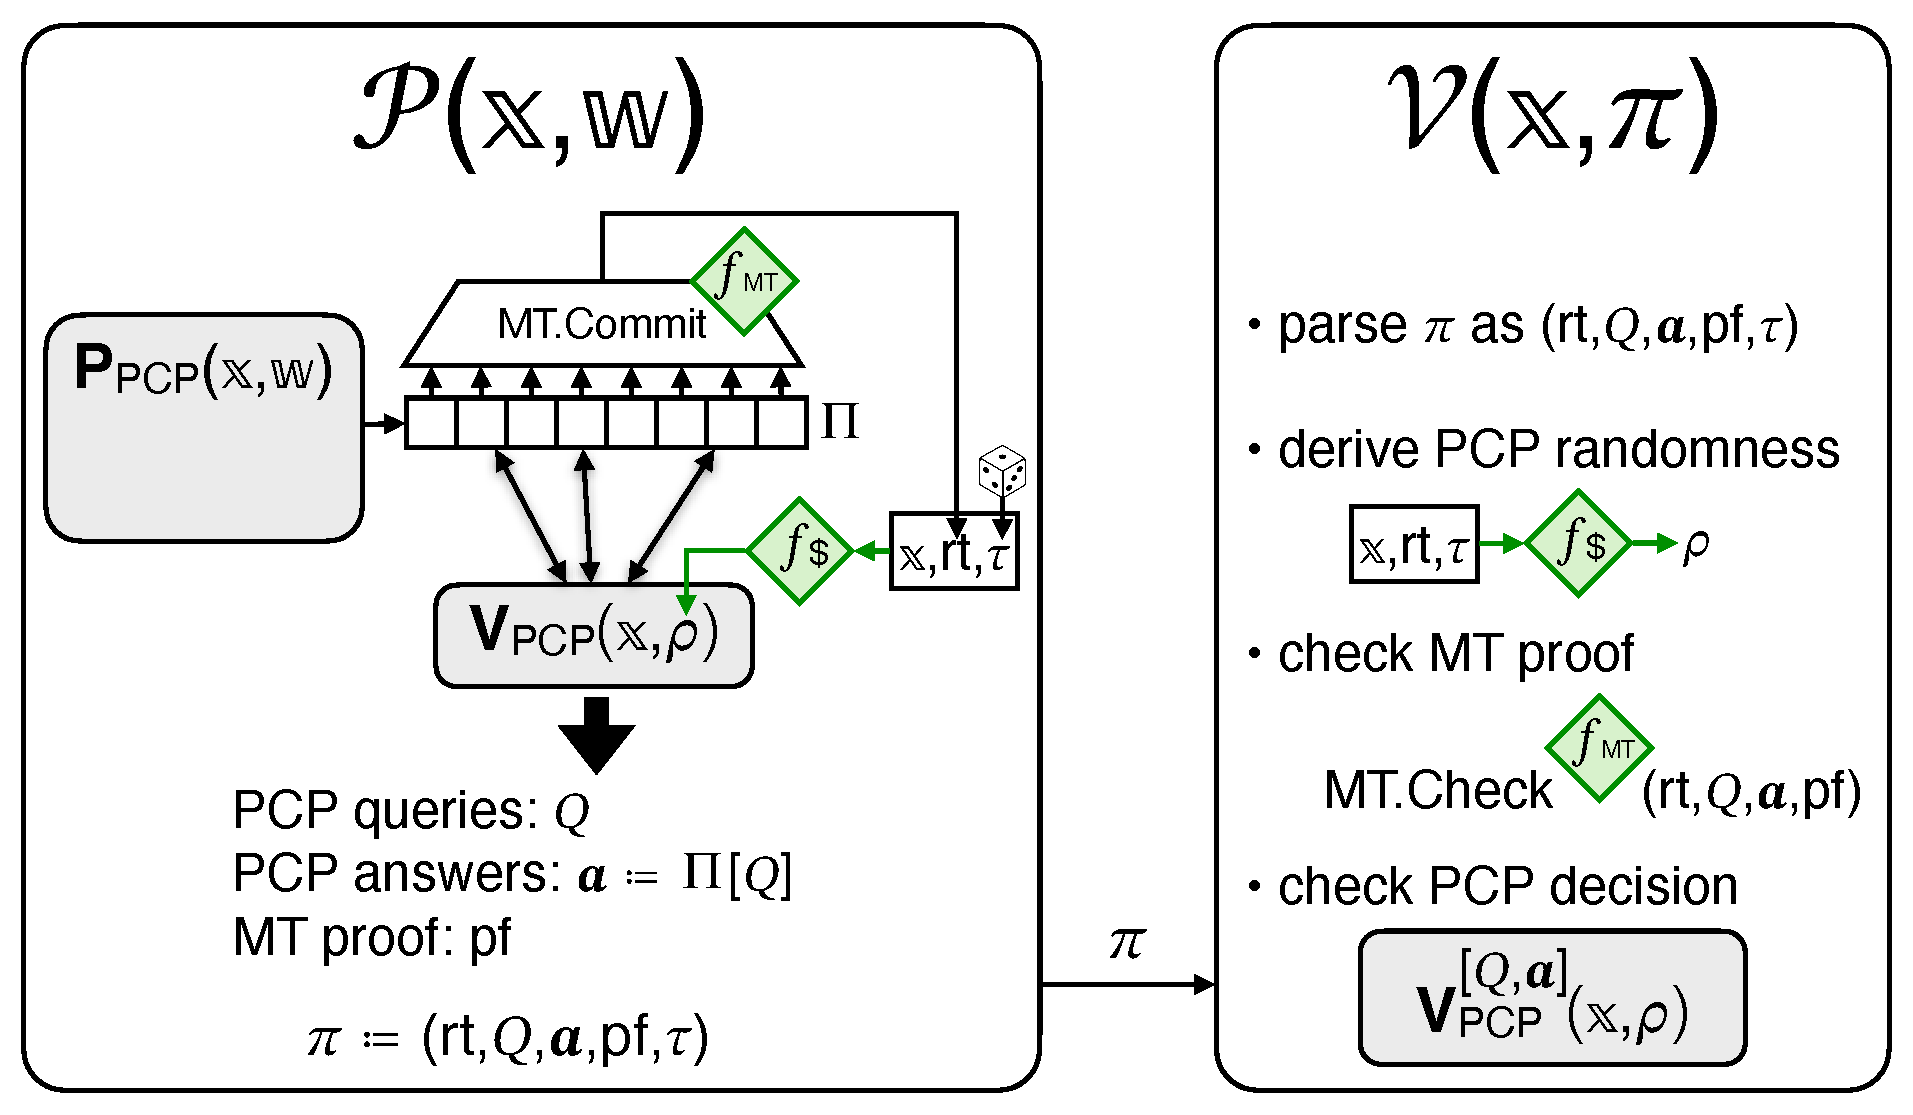
\includegraphics[width=0.8\textwidth]{\FigureFolder/micali-diagram}
\caption[Diagram of the Micali transformation]{Diagram of the \MicaliText ($\MicaliSymbol$ in \Cref{construction:micali-transformation}).}
\label{figure:micali-diagram}
\end{figure}

%%%%%%%%%%%%%%%%%%%%%%%%%%%%%%%%%%%%%%%%%%%%%%%%%%%%%%%%%%%%%%%%%%%%%%%%%%%%%%%
%%%%%%%%%%%%%%%%%%%%%%%%%%%%%%%%%%%%%%%%%%%%%%%%%%%%%%%%%%%%%%%%%%%%%%%%%%%%%%%
%%%%%%%%%%%%%%%%%%%%%%%%%%%%%%%%%%%%%%%%%%%%%%%%%%%%%%%%%%%%%%%%%%%%%%%%%%%%%%%
\section{Soundness}
\label{section:micali-soundness}

We prove that \Cref{construction:micali-transformation} is (adaptively) sound. The following theorem states that the (adaptive) soundness error of the non-interactive argument against a $\ROQueryBound$-query argument prover is upper bounded by the soundness error of the underlying PCP \emph{multiplied by $\ROQueryBound+1$} plus a small term. This latter term represents the error term incurred by \DoQuote{breaking} the Merkle commitment scheme used to commit to the PCP string.

\begin{ImportantTheorem}{}{micali-soundness}
Let $\PCPSymbol$ be a PCP for a relation $\Relation$ with soundness error $\PCPSoundnessError$ and proof length $\PCPProofLength$. For every security parameter $\SecurityParameter \in \Naturals$ and privacy parameter $\PrivacyParameter \in \Naturals$, $\NARGSymbol \DefineEqual \MicaliTransformation{\PCPSymbol}{\SecurityParameter}{\PrivacyParameter}$ in \Cref{construction:micali-transformation} is a non-interactive argument for $\Relation$ with adaptive soundness error $\ARGSoundnessError$ (see \Cref{definition:narg-adaptive-soundness-with-cnf}) such that
\begin{equation*}
\ARGSoundnessError(\SecurityParameter,\ROQueryBound,\InstanceSize)
\leq
\MicaliSoundnessExpression
\enspace.
\end{equation*}
Above $\MTMultiExtractionError$ is the Merkle commitment multi-extraction error from \Cref{lemma:mt-multi-extractability}, and $\MTMultiExtractionError(\SecurityParameter,\ROQueryBound,\PCPProofLength,\ROQueryBound+1,1) \leq \MTMultiExtractabilityShortExpression{\SecurityParameter}{\ROQueryBound}$ if $\MTMultiExtractabilityCondition{\ROQueryBound}{1}{\log\PCPProofLength}$.
\end{ImportantTheorem}

The soundness error in \Cref{theorem:micali-soundness} (soundness of the Micali transformation) differs from the soundness error in \Cref{theorem:kilian-adaptive-soundness} (soundness of the Kilian transformation) in two ways:
\begin{itemize}[noitemsep]
  \item the PCP soundness error $\PCPSoundnessError(\InstanceSize)$ is multiplied by $(\ROQueryBound+1)$; and
  \item the additive error arising from \DoQuote{breaking} the Merkle commitment scheme is a multi-extraction error (one opening out of $\ROQueryBound+1$ commitments) rather than a single-extraction error.
\end{itemize}
In particular, for the same level of desired security, a PCP must be $(\ROQueryBound+1)$ times \DoQuote{sounder} to be used in the Micali transformation when compared to in the Kilian transformation.

The above differences come from the fact that in the Kilian transformation an argument prover has a single opportunity to attack the underlying PCP: after sending to the argument verifier a Merkle commitment $\MTCommitment$, the argument prover receives PCP randomness from the argument verifier, and has to open the requested locations in a way that is consistent with the Merkle commitment.

In contrast, in the Micali transformation, the argument prover can explore different choices of PCP randomness for different choices of Merkle commitments (in fact, even for the same Merkle commitment by changing the salt), because each PCP randomness is obtained as the answer to a certain query to the random oracle. Each such exploration costs a query, so a $\ROQueryBound$-query argument prover can see at most $\ROQueryBound$ choices of PCP randomness; in fact, the argument prover can also output a Merkle commitment for which it did not query the random oracle (and hence for which it did not see the corresponding PCP randomness). This informally justifies the term $(\ROQueryBound+1) \cdot \PCPSoundnessError(\InstanceSize)$ in the soundness error expression. The other term in the soundness error expression denotes the fact that in the security reduction we extract a PCP string from the Merkle commitment, out of up to $\ROQueryBound+1$ explored by the argument prover, that the argument prover outputs in the argument string. This is a multi-extraction error, unlike in the case of the Kilian transformation.

The above phenomenon is analogous to what happens in the Fiat--Shamir transformation for SPs (see \Cref{chapter:fiat-shamir-transformation-for-sp}), wherein the soundness error of the resulting non-interactive argument is $\ROQueryBound+1$ times the SP soundness error. No other error terms appear because no Merkle commitment schemes are used in that case.

Analyzing the Micali transformation as the \DoQuote{black-box} application of the Fiat--Shamir transformation to the Kilian transformation does not lead to an asymptotically tight result. (See \Cref{remark:micali-from-fs-applied-to-killian}.) Instead, we analyze the Micali transformation directly: \Cref{theorem:micali-soundness} directly follows from the lemma below. We separately bound the number $\RORandQueryBound$ of queries to the (derived) oracle $\RORandFunction$ and the number $\ROTreeQueryBound$ of queries to the (derived) oracle $\ROTreeFunction$. Both are upper bounded by the number $\ROQueryBound$ of queries to the random oracle $\ROFunction$.

\begin{lemma}
\label{lemma:micali-adaptive-reduction}
There exists a PCP prover $\PCPMaliciousProver$ such that for every $(\ROTreeQueryBound,\RORandQueryBound)$-query argument prover $\Malicious{\ARGProver}$ the following holds for every instance size bound $\InstanceSize \in \Naturals$:
\begin{align*}
&\Pr\left[
\begin{array}{l}
  \SomeSize{\Instance} \leq \InstanceSize \\
  \land\;\Instance \notin \GetLanguage{\Relation} \\
  \land\;\ARGVerifier^{\ROFunction}(\Instance,\ARGString)=1
\end{array}
\GivenExperiment
\StateExperiment{
  \ROFunction=(\ROTreeFunction,\RORandFunction) \gets \RODistribution{(\SecurityParameter,\PCPRandomnessComplexity)} \\
  (\Instance,\ARGString) \gets \Malicious{\ARGProver}^{\ROFunction}
}
\right]
\\ & \leq
(\RORandQueryBound+1) \cdot
\Pr\left[
\begin{array}{l}
  \SomeSize{\Instance} \leq \InstanceSize \\
  \land\;\Instance \notin \GetLanguage{\Relation} \\
  \land\;\PCPVerifier^{\PCPString}(\Instance,\PCPVerifierRandomMessage)=1
\end{array}
\GivenExperiment
\StateExperiment{
  (\Instance,\PCPString) \gets \PCPMaliciousProver(\BlackBox{\ARGProver}) \\
  \PCPVerifierRandomMessage \gets \Bits^{\PCPRandomnessComplexity}
}
\right]
+
\MTMultiExtractionError(\SecurityParameter,\ROTreeQueryBound,\PCPProofLength,\RORandQueryBound+1,1)
\enspace.
\end{align*}
\end{lemma}

We state a claim that reduces the argument prover to a PCP state-restoration prover, up to a multi-extraction error. Then we prove the lemma by using the fact that PCP state-restoration soundness can be related to the PCP's (standard) soundness.

While the state-restoration game has a formal output, for the purpose of analysis we externalize certain quantities introduced during the execution of the game. We place these quantities under the arrow that leads to the game output. Specifically, in the claim below, we consider a query-answer trace $\ROTreeTrace$ and a bit $\DecisionBit_{\MTSubscript}$, which are set by the PCP state-restoration prover $\PCPMaliciousSRProver$ that we construct.

\begin{claim}
\label{claim:micali-reduction}
There exists a PCP state-restoration prover $\PCPMaliciousSRProver$ such that, for every $(\ROTreeQueryBound,\RORandQueryBound)$-query argument prover $\Malicious{\ARGProver}$, $\PCPMaliciousSRProver$ makes at most $\RORandQueryBound$ moves and the following two distributions are $\MTMultiExtractionError(\SecurityParameter,\ROTreeQueryBound,\PCPProofLength,\RORandQueryBound+1,1)$-close in statistical distance
\begin{align*}
&
\left\{
  (\ROTreeTrace,\Instance,\PCPString,b)
\GivenExperiment
\StateExperiment{
  \ROFunction=(\ROTreeFunction,\RORandFunction) \gets \RODistribution{(\SecurityParameter,\PCPRandomnessComplexity)} \\
  \ROOutputAndTrace{\ROFunction}{\Malicious{\ARGProver}}{\ROTrace}{(\Instance,\ARGString=\MicaliARGString)} \\
(\PCPString, \MTTrapdoor) \gets \MTExtractor(\MTCommitment, \ROTreeTrace) \\
  b = \ARGVerifier^{\ROFunction}(\Instance,\ARGString)
}
\right\}
\quad \text{and} \quad
\\ &
\left\{
  (\ROTreeTrace,\Instance,\PCPString,b)
\GivenExperiment
\StateExperiment{
  \ROFunction=(\ROTreeFunction,\RORandFunction) \gets \RODistribution{(\SecurityParameter,\PCPRandomnessComplexity)} \\
  \ShortExecutionBelow{(\Instance,\PCPString,\SRSaltString,\PCPVerifierRandomMessage)}{\PCPStateRestorationGame{\SecurityParameter+\RandSaltSize}{\RORandFunction} {(\PCPMaliciousSRProver(\BlackBox{\Malicious{\ARGProver}}))^{\ROTreeFunction}}}{\ROTreeTrace,\DecisionBit_{\MTSubscript}} \\
  b \DefineEqual \PCPVerifier^{\PCPString}(\Instance,\PCPVerifierRandomMessage) \land \DecisionBit_{\MTSubscript}
}
\right\}
\enspace.
\end{align*}
Moreover, the running time of $\PCPMaliciousSRProver$ equals the running time of $\Malicious{\ARGProver}$ plus $\MTMultiExtractorTimeFunction{\SecurityParameter}{\PCPAlphabet}{\PCPProofLength}{\PrivacyParameter}{\ROTreeQueryBound}{\RORandQueryBound+1}$ where $\MTMultiExtractorTimeSymbol$ is the time complexity of the Merkle commitment multi-extractor in \Cref{lemma:mt-multi-extractability}.
\end{claim}

\begin{construction}
\label{construction:micali-reduction}
Let $\MTMultiExtractor$ be the Merkle commitment multi-extractor for $\MTSymbol$ from \Cref{lemma:mt-multi-extractability} in \Cref{section:merkle-commitment-multi-extractability}. The PCP state-restoration prover $\PCPMaliciousSRProver \DefineEqual \PCPMaliciousSRProver(\BlackBox{\Malicious{\ARGProver}})$ works as follows.
\begin{enumerate}[noitemsep]
  \item Lazily sample an oracle $\Lazy{\ROFunctionAlt} \gets \RODistribution{\PCPRandomnessComplexity}$ (to be used as auxiliary randomness).
  \item Initialize an empty query-answer trace $\ROTreeTrace$.
  \item Simulate $\Malicious{\ARGProver}$ while answering its queries as described below.
  \item When $\Malicious{\ARGProver}$ performs a query to the oracle $\ROTreeFunction$, answer according to $\ROTreeFunction$ and append the resulting query-answer pair to $\ROTreeTrace$.
  \item When $\Malicious{\ARGProver}$ performs the $\SRIteration$-th query $\ROQuery_{\SRIteration}$ to the oracle $\RORandFunction$, do the following:
  \begin{enumerate}[nolistsep]
    \item If $\ROQuery_{\SRIteration}$ can be parsed as a tuple $(\Instance_{\SRIteration},\MTCommitment_{\SRIteration},\RandSaltString_{\SRIteration})$ where $\Instance_{\SRIteration}$ is an instance, $\MTCommitment_{\SRIteration}$ a Merkle commitment, and $\RandSaltString_{\SRIteration}$ a salt string:
  \begin{enumerate}[noitemsep]
    \item Let $\ROTrace_{\SRIteration} \subseteq \ROTreeTrace$ be the query-answer pairs for $\ROTreeFunction$ between the previous iteration and the current iteration (or the beginning if this is the first iteration).
    \item \label{micali-step:mt-extractor}
    Run the Merkle extractor: $(\PCPString_{\SRIteration},\MTTrapdoor_{\SRIteration}) \DefineEqual \MTMultiExtractor(\MTCommitment_{\SRIteration},\ROTrace_{\SRIteration})$.
    \item Set the salt string $\SRSaltString_{\SRIteration} \DefineEqual (\MTCommitment_{\SRIteration},\RandSaltString_{\SRIteration})$.
    \item Submit in \Cref{step:pcp-srgame-loop-output} of the game the move $(\Instance_{\SRIteration},\PCPString_{\SRIteration},\SRSaltString_{\SRIteration})$. \label{step:SRGame-pcp-perform-move}
    \item Receive PCP randomness $\PCPVerifierRandomMessage_{\SRIteration} \in \Bits^{\PCPRandomnessComplexity}$ from the game. \label{step:SRGame-pcp-randomness}
  \end{enumerate}
    \item Otherwise set $\PCPVerifierRandomMessage_{\SRIteration} \DefineEqual \Lazy{\ROFunctionAlt}(\ROQuery_{\SRIteration})$.
    \item Return $\PCPVerifierRandomMessage_{\SRIteration}$ to $\Malicious{\ARGProver}$ as the answer to its query.
  \end{enumerate}
  \item Let $(\Instance,\ARGString)$ be the output of $\Malicious{\ARGProver}$ when it halts, and parse $\ARGString$ as $\MicaliARGString$.
  \item Let $\ROTrace' \subseteq \ROTreeTrace$ be the query-answer pairs for $\ROTreeFunction$ between the last iteration and $\Malicious{\ARGProver}$'s halting.
  \item \label{micali-step:mt-extractor-final} Run the Merkle extractor to obtain a PCP string: $(\PCPString,\MTTrapdoor) \DefineEqual \MTMultiExtractor(\MTCommitment,\ROTrace')$.
  \item Set the salt string $\SRSaltString \DefineEqual (\MTCommitment,\RandSaltString)$.
  \item Set $\DecisionBit_{\MTSubscript} \DefineEqual \MTCheck^{\ROTreeFunction}(\MTCommitment,\PCPQuerySet,\MTMessageSubVector,\MTProof)$. (This bit is only used in the analysis.)
  \item Output $(\Instance,\PCPString,\SRSaltString)$.
\end{enumerate}
The prover $\PCPMaliciousSRProver$ potentially makes a move (in \Cref{step:SRGame-pcp-perform-move}) for every query of $\Malicious{\ARGProver}$ to the oracle $\RORandFunction$ (no other moves are performed). Since there are at most $\RORandQueryBound$ queries to $\RORandFunction$, we get that $\PCPMaliciousSRProver$ performs at most $\RORandQueryBound$ moves. In terms of running time, $\PCPMaliciousSRProver$ simulates $\Malicious{\ARGProver}$ (which takes the running time of $\Malicious{\ARGProver}$) and additionally performs at most $\RORandQueryBound+1$ Merkle commitment extractions (at most once per query of $\Malicious{\ARGProver}$ to $\RORandFunction$ plus an additional one for the output of $\Malicious{\ARGProver}$). The total time for all extractions is given by the expression $\MTMultiExtractorTimeFunction{\SecurityParameter}{\PCPAlphabet}{\PCPProofLength}{\PrivacyParameter}{\ROTreeQueryBound}{\RORandQueryBound+1}$ where $\MTMultiExtractorTimeSymbol$ is the (total) time complexity of $\MTMultiExtractor$ in \Cref{lemma:mt-multi-extractability}. Hence the running time of $\PCPMaliciousSRProver$ is as in the claim.
\end{construction}

\begin{proof}[Proof of \Cref{claim:micali-reduction}]
We define an event $\Event$ over the probability space of sampling a random oracle $\ROFunction=(\ROTreeFunction,\RORandFunction) \gets \RODistribution{(\SecurityParameter,\PCPRandomnessComplexity)}$, running $\ROOutputAndTrace{\ROFunction}{\Malicious{\ARGProver}}{\ROTrace}{(\Instance,\ARGString=\MicaliARGString)}$ (as in the top distribution of the claim statement), and then running $\PCPStateRestorationGame{\SecurityParameter+\RandSaltSize}{\RORandFunction}{(\PCPMaliciousSRProver(\BlackBox{\Malicious{\ARGProver}}))^{\ROTreeFunction}}$ (as in the bottom distribution of the claim statement). The event $\Event$ is as follows:
\begin{enumerate}[noitemsep]
  \item $\ARGVerifier^{\ROFunction}(\Instance,\ARGString)=1$ and $\PCPString[\PCPQuerySet] \neq \PCPEntries$ (the argument verifier accepts but the Merkle commitment multi-extractor fails in extracting a corresponding PCP string in \Cref{micali-step:mt-extractor-final}); OR
  \item there exists $\SRIteration, \SRIteration' \in [\RORandQueryBound]$ such that $\MTCommitment_{\SRIteration} = \MTCommitment_{\SRIteration'}$ but $\PCPString_{\SRIteration} \neq \PCPString_{\SRIteration'}$ (the Merkle commitment multi-extractor outputs two different strings on the same Merkle commitment but with different query-answer traces).
\end{enumerate}
It suffices to upper bound the probability that $\Event$ holds and showing that the following two distributions (which additionally include the randomness $\PCPVerifierRandomMessage$) are identical:
\begin{align*}
&
\left\{
\begin{array}{l}
  (\ROTreeTrace,\PCPVerifierRandomMessage,\Instance,\PCPString,\DecisionBit) \\
    \ConditionedOnText \\
    \Negate{\Event}
\end{array}
\GivenExperiment
\StateExperiment{
  \ROFunction=(\ROTreeFunction,\RORandFunction) \gets \RODistribution{(\SecurityParameter,\PCPRandomnessComplexity)} \\
  \ROOutputAndTrace{\ROFunction}{\Malicious{\ARGProver}}{\ROTrace}{(\Instance,\ARGString=\MicaliARGString)} \\
  (\PCPString, \MTTrapdoor) \gets \MTExtractor(\MTCommitment, \ROTreeTrace) \\
  \DecisionBit \DefineEqual \ARGVerifier^{\ROFunction}(\Instance,\ARGString) \\
  \PCPVerifierRandomMessage \DefineEqual \RORandFunction\MicaliFSQuery
}
\right\}
\\ &
\equiv
\\ &
\left\{
\begin{array}{l}
 (\ROTreeTrace,\PCPVerifierRandomMessage,\Instance,\PCPString,\DecisionBit) \\
\ConditionedOnText \\
\Negate{\Event}
\end{array}
\GivenExperiment
\StateExperiment{
  \ROFunction=(\ROTreeFunction,\RORandFunction) \gets \RODistribution{(\SecurityParameter,\PCPRandomnessComplexity)} \\
  \ShortExecutionBelow{(\Instance,\PCPString,\SRSaltString,\PCPVerifierRandomMessage)}{\PCPStateRestorationGame{\SecurityParameter+\RandSaltSize}{\RORandFunction}{(\PCPMaliciousSRProver(\BlackBox{\Malicious{\ARGProver}}))^{\ROTreeFunction}}}{\ROTreeTrace,\DecisionBit_{\MTSubscript}} \\
  \DecisionBit \DefineEqual \PCPVerifier^{\PCPString}(\Instance,\PCPVerifierRandomMessage) \land \DecisionBit_{\MTSubscript}
}
\right\}
\enspace.
\end{align*}
Below we refer to the two experiments as the left-side experiment (the one to the left of the equality) and the right-side experiment (the one to the right of the equality). Both experiments involve the execution (or emulation) of $\Malicious{\ARGProver}$.

First we argue that the distribution of \emph{answers} to oracle queries are identical in both experiments.
\begin{itemize}

\item \emph{Queries to the oracle $\ROTreeFunction$.}
In the left-side experiment $\Malicious{\ARGProver}$ directly queries $\ROTreeFunction$, while in the right-side experiment $\Malicious{\ARGProver}$ queries $\ROTreeFunction$ through $\PCPMaliciousSRProver$ (which emulates $\Malicious{\ARGProver}$ and has query access to $\ROTreeFunction$). Both experiments are conditioned on the same event $\Negate{\Event}$. We conclude that the distribution of the query-answer trace $\ROTreeTrace$ is identical in both experiments.

\item \emph{Queries to the oracle $\RORandFunction$.}
In the left-side experiment, $\Malicious{\ARGProver}$ directly queries $\RORandFunction$, receiving corresponding answers, conditioned on the event $\Negate{\Event}$.

In the right-side experiment, $\RORandFunction$ is given as the auxiliary randomness $\SRRandomness$ in the PCP state-restoration game, and queries of $\Malicious{\ARGProver}$ to $\RORandFunction$ are translated to moves of $\PCPMaliciousSRProver$ or forwarded to the (lazily sampled) oracle $\Lazy{\ROFunctionAlt}$. Specifically, if a query $\ROQuery_{\SRIteration}$ to $\RORandFunction$ has the form $(\Instance_{\SRIteration},\MTCommitment_{\SRIteration},\RandSaltString_{\SRIteration})$ then it receives the answer $\SRRandomness(\Instance_{\SRIteration},\PCPString_{\SRIteration}, \SRSaltString_{\SRIteration})=\RORandFunction(\Instance_{\SRIteration},\PCPString_{\SRIteration}, \SRSaltString_{\SRIteration})$ for $\SRSaltString_{\SRIteration} = (\MTCommitment_{\SRIteration},\RandSaltString_{\SRIteration})$; otherwise, it receives the answer $\Lazy{\ROFunctionAlt}(\ROQuery_{\SRIteration})$. All answers are conditioned on the event $\Negate{\Event}$.

Every unique query $\ROQuery_{\SRIteration}$ is mapped to a unique PCP state-restoration move $(\Instance_{\SRIteration},\PCPString_{\SRIteration}, \SRSaltString_{\SRIteration})$ or to a unique input to $\Lazy{\ROFunctionAlt}$. Moreover, any duplicate query is mapped to the same move in the PCP state-restoration game or the same input to $\Lazy{\ROFunctionAlt}$. The latter case is clear but the former case follows from the fact that $\Event$ does not hold, as we now explain. Assume that rounds $\SRIteration$ and $\SRIteration'$ are duplicate queries that can be parsed as identical tuples $(\Instance_{\SRIteration},\MTCommitment_{\SRIteration},\RandSaltString_{\SRIteration})$ and $(\Instance_{\SRIteration'},\MTCommitment_{\SRIteration'},\RandSaltString_{\SRIteration'})$. The mapped queries are identical except (potentially) the strings $\PCPString_{\SRIteration}$ and $\PCPString_{\SRIteration'}$. However both are extracted from the same Merkle commitment $\MTCommitment_{\SRIteration}=\MTCommitment_{\SRIteration'}$, so it must be that $\PCPString_{\SRIteration}=\PCPString_{\SRIteration'}$: if $\PCPString_{\SRIteration} \neq \PCPString_{\SRIteration'}$ then this would contradict the assumption that $\Event$ does not hold. Note that while queries to $\ROTreeFunction$ are the same in both experiments, queries to $\RORandFunction$ (in the left-side experiment) differ from moves in the PCP state-restoration game (in the right-side experiment).

\end{itemize}
Next, given that $\Malicious{\ARGProver}$ sees the same distribution of answers, we argue that all elements in $(\ROTreeTrace, \PCPVerifierRandomMessage, \Instance, \PCPString, b)$ have the same distribution in both experiments.
\begin{itemize}

\item \emph{Distribution of $\Instance,\PCPString$.}
Since $\Malicious{\ARGProver}$ receives answers that have the same distribution in both experiments (as argued above), its output $(\Instance,\ARGString)$ has the same distribution in both experiments as well. Recall that $\ARGString = \MicaliARGString$ and that $(\PCPString, \MTTrapdoor) \gets \MTExtractor(\MTCommitment, \ROTreeTrace)$. Since $\ROTreeTrace$ is identical in both experiments, we conclude that $\PCPString$ is identical as well.

\item \emph{Distribution of $\PCPVerifierRandomMessage$.}
For the same reasons as the answer of the queries, $\PCPVerifierRandomMessage$ is identically distributed in both experiments. If the query-answer pair $(\MicaliFSQuery,\PCPVerifierRandomMessage)$ was already performed, then since the answers to $\RORandFunction$ are uniformly distributed we have that $\PCPVerifierRandomMessage$ is uniformly distributed in both sides. Otherwise, the query-answer pair $(\MicaliFSQuery,\PCPVerifierRandomMessage)$ can be viewed as an additional query, which by the same argument is uniformly distributed.

\item \emph{Distribution of the bit $\DecisionBit$.}
The bit $\DecisionBit$ is a function of $(\Instance,\PCPVerifierRandomMessage,\ARGString)$ in the left-side experiment and is a function of $(\Instance,\PCPVerifierRandomMessage,\PCPString,\DecisionBit_{\MTSubscript})$ in the right-side experiment. We show that $\DecisionBit=1$ on the left-side experiment implies that $\DecisionBit=1$ on the right-side experiment, and the same holds for $\DecisionBit=0$.

If $\ARGVerifier^{\ROFunction}(\Instance,\ARGString)=1$ ($\DecisionBit=1$ in the left-side experiment) then we know that: $\PCPVerifier^{\PCPLocalView{\PCPQuerySet}{\PCPEntries}}(\Instance,\PCPVerifierRandomMessage)=1$ and $\MTCheck^{\ROTreeFunction}(\MTCommitment,\PCPQuerySet,\MTMessageSubVector,\MTProof)=1$. Since the event $\Event$ does not hold, this implies that $\PCPString[\PCPQuerySet] = \PCPEntries$, which in turn implies that $\PCPVerifier^{\PCPString}(\Instance,\PCPVerifierRandomMessage) = 1$. Since $\MTCheck^{\ROTreeFunction}(\MTCommitment,\PCPQuerySet,\MTMessageSubVector,\MTProof)=1$ we have that $\DecisionBit_{\MTSubscript}=1$ in the right-side experiment. Overall, we get that $\DecisionBit=1$ in the right-side experiment.

If $\ARGVerifier^{\ROFunction}(\Instance,\ARGString)=0$ ($\DecisionBit=0$ in the left-side experiment), then either:
\begin{inparaenum}[(a)]
  \item $\PCPVerifier^{\PCPLocalView{\PCPQuerySet}{\PCPEntries}}(\Instance,\PCPVerifierRandomMessage)=0$; or
  \item $\MTCheck^{\ROTreeFunction}(\MTCommitment,\PCPQuerySet,\MTMessageSubVector,\MTProof)=0$.
\end{inparaenum}
If $\MTCheck^{\ROTreeFunction}(\MTCommitment,\PCPQuerySet,\MTMessageSubVector,\MTProof)=0$ then $\DecisionBit_{\MTSubscript} = 0$. Otherwise $\MTCheck^{\ROTreeFunction}(\MTCommitment,\PCPQuerySet,\MTMessageSubVector,\MTProof)=1$ and $\PCPVerifier^{\PCPLocalView{\PCPQuerySet}{\PCPEntries}}(\Instance,\PCPVerifierRandomMessage)=0$, which implies that $\PCPString[\PCPQuerySet] = \PCPEntries$ (as else we would have $\MTCheck^{\ROTreeFunction}(\MTCommitment,\PCPQuerySet,\MTMessageSubVector,\MTProof)=0$), which means that $\PCPVerifier^{\PCPString}(\Instance,\PCPVerifierRandomMessage) = 0$. In both cases $\DecisionBit=0$ in the right-side experiment.

\end{itemize}

Finally, we are left to upper bound the probability of the event $\Event$. This is straightforward via \Cref{lemma:mt-multi-extractability}, which considers \emph{extraction from multiple commitments}. Indeed, we invoke the Merkle commitment multi-extractor $\MTMultiExtractor$ multiple times, each time on a (possibly) different root $\MTCommitment_{\SRIteration}$ with trace $\ROTrace_{\SRIteration}$ (recall that $\MTMultiExtractor$ is a stateful algorithm). According to the lemma, the probability that there exists an execution for which $\MTMultiExtractor$ does not succeed (but for which the adversary outputs a valid proof) is upper bounded by $\MTMultiExtractionError(\SecurityParameter,\ROTreeQueryBound,\PCPProofLength,\RORandQueryBound+1,1)$. Here the function $\MTMultiExtractionError$ gets five parameters: $\SecurityParameter$ is the security parameter, $\ROTreeQueryBound$ is the query bound, $\PCPProofLength$ is the length of the PCP string $\PCPString$, $\RORandQueryBound+1$ is the number of output Merkle commitments, and $1$ is the number of opened Merkle commitments (the argument prover opens one of the output commitments).
\end{proof}

\begin{proof}[Proof of \Cref{lemma:micali-adaptive-reduction}]
The probability statement on the left-side of the inequality is a function of the instance $\Instance$ and the bit $\DecisionBit = \ARGVerifier^{\ROFunction}(\Instance,\ARGString)$, generated from a random experiment. Using \Cref{claim:micali-reduction}, we can switch the experiment with the argument prover for the corresponding experiment with the state-restoration prover, the same instance, and the bit $\DecisionBit=\PCPVerifier^{\PCPString}(\Instance,\PCPVerifierRandomMessage) \land \DecisionBit_{\MTSubscript}$.

Hence we get that the probability in the lemma statement can be upper bounded as follows:
\begin{align*}
&\Pr\left[
\begin{array}{l}
  \SomeSize{\Instance} \leq \InstanceSize \\
  \land\;\Instance \notin \GetLanguage{\Relation} \\
  \land\;\ARGVerifier^{\ROFunction}(\Instance,\ARGString)=1
\end{array}
\GivenExperiment
\StateExperiment{
  \ROFunction=(\ROTreeFunction,\RORandFunction) \gets \RODistribution{(\SecurityParameter,\PCPRandomnessComplexity)} \\
  (\Instance,\ARGString) \gets \Malicious{\ARGProver}^{\ROFunction}
}
\right]
\\ & \leq
\Pr\left[
\begin{array}{l}
\SomeSize{\Instance} \leq \InstanceSize \\
\land\;\Instance \notin \GetLanguage{\Relation} \\
\land\;\PCPVerifier^{\PCPString}(\Instance,\PCPVerifierRandomMessage) = 1\\
\land\;\DecisionBit_{\MTSubscript}=1
\end{array}
\GivenExperiment
\StateExperiment{
\ROFunction=(\ROTreeFunction,\RORandFunction) \gets \RODistribution{(\SecurityParameter,\PCPRandomnessComplexity)} \\
\ShortExecutionBelow{(\Instance,\PCPString,\SRSaltString,\PCPVerifierRandomMessage)}{\PCPStateRestorationGame{\SecurityParameter+\RandSaltSize}{\RORandFunction} {(\PCPMaliciousSRProver)^{\ROTreeFunction}}}
{\DecisionBit_{\MTSubscript}} \\
}
\right]
\\ & \quad\quad +
\MTMultiExtractionError(\SecurityParameter,\ROTreeQueryBound,\PCPProofLength,\RORandQueryBound+1,1)
\EquationComment{by \Cref{claim:micali-reduction}}
\\ & \leq
\Pr\left[
\begin{array}{l}
\SomeSize{\Instance} \leq \InstanceSize \\
\land\;\Instance \notin \GetLanguage{\Relation} \\
\land\;\PCPVerifier^{\PCPString}(\Instance,\PCPVerifierRandomMessage) = 1
\end{array}
\GivenExperiment
\StateExperiment{
\ROFunction=(\ROTreeFunction,\RORandFunction) \gets \RODistribution{(\SecurityParameter,\PCPRandomnessComplexity)} \\
\ShortExecution{(\Instance,\PCPString,\SRSaltString,\PCPVerifierRandomMessage)}{\PCPStateRestorationGame{\SecurityParameter+\RandSaltSize}{\RORandFunction} {(\PCPMaliciousSRProver)^{\ROTreeFunction}}} \\
}
\right]
\\ & \quad\quad +
\MTMultiExtractionError(\SecurityParameter,\ROTreeQueryBound,\PCPProofLength,\RORandQueryBound+1,1)
\EquationComment{by dropping the condition $\DecisionBit_{\MTSubscript}=1$}
\enspace.
\end{align*}
Above $\PCPMaliciousSRProver \DefineEqual \PCPMaliciousSRProver(\BlackBox{\Malicious{\ARGProver}})$ is the PCP state-restoration prover obtained from $\Malicious{\ARGProver}$ in the claim. The argument prover $\Malicious{\ARGProver}$ makes at most $\RORandQueryBound$ queries to $\RORandFunction$, so $\PCPMaliciousSRProver$ makes at most $\RORandQueryBound$ moves, and so (by \Cref{definition:pcp-state-restoration-soundness}) the above probability is upper bounded by the following expression:
\begin{equation*}
\PCPSRSoundnessError(\SecurityParameter+\RandSaltSize,\RORandQueryBound,\InstanceSize)
+ \MTMultiExtractionError(\SecurityParameter,\ROTreeQueryBound,\PCPProofLength,\RORandQueryBound+1,1)
\enspace.
\end{equation*}
By \Cref{theorem:pcp-srs-to-soundness} (which bounds PCP state-restoration soundness error in terms of soundness error), the above probability is upper bounded by the following expression:
\begin{equation*}
(\RORandQueryBound+1) \cdot
\Pr\left[
\begin{array}{l}
  \SomeSize{\Instance} \leq \InstanceSize \\
  \land\;\Instance \notin \GetLanguage{\Relation} \\
  \land\;\PCPVerifier^{\PCPString}(\Instance,\PCPVerifierRandomMessage)=1
\end{array}
\GivenExperiment
\StateExperiment{
  (\Instance,\PCPString) \gets \PCPMaliciousProver \\
  \PCPVerifierRandomMessage \gets \Bits^{\PCPRandomnessComplexity}
}
\right]
+ \MTMultiExtractionError(\SecurityParameter,\ROTreeQueryBound,\PCPProofLength,\RORandQueryBound+1,1)
\enspace.
\end{equation*}
Above, $\PCPMaliciousProver \DefineEqual \PCPMaliciousProver(\SRSaltSize,\SRBudget,\BlackBox{\PCPMaliciousSRProver})$ is the PCP prover obtained from \Cref{theorem:pcp-srs-to-soundness}.
\end{proof}

\begin{remark}[alternative soundness analysis]
\label{remark:micali-from-fs-applied-to-killian}
In \Cref{section:micali-construction} we explain how the Micali transformation can be viewed as the Fiat--Shamir transformation for SPs applied to the ($3$-message public-coin) interactive argument resulting from the Kilian transformation (applied to the PCP).

So why does the above soundness analysis not follow this structure? (We do not simply combine the soundness guarantees of the Fiat--Shamir transformation and of the Kilian transformation.)

One issue is that we would need to extend the soundness analysis of the Fiat--Shamir transformation to work for a relaxation of SPs that are interactive arguments. The Kilian transformation outputs a protocol with the structure of an SP but with weaker soundness: it is an interactive argument rather than an interactive proof. That said, this extension could be carried out, which would lead to a modular analysis of the Micali transformation, resolving this particular issue.

There is another, more important, issue though. A modular analysis based on the two transformations would incur an undesirable overhead in soundness error, as we now explain. The Kilian transformation has a soundness error that is the sum of the PCP soundness error and a Merkle commitment single-extraction error. The Fiat--Shamir transformation for SPs (and relaxations thereof) has a soundness error that is $\RORandQueryBound+1$ times the soundness error of the SP. Overall this would establish a soundness error for the Micali transformation that is
\begin{equation*}
(\RORandQueryBound+1)
\cdot
\left(
\PCPSoundnessError(\InstanceSize)
+
\MTExtractionError(\SecurityParameter,\ROTreeQueryBound,\PCPProofLength)
\right)
\enspace.
\end{equation*}
However, the upper bound that we establish for the Micali transformation is better:
\begin{equation*}
(\RORandQueryBound+1) \cdot \PCPSoundnessError(\InstanceSize)
+
\MTMultiExtractionError(\SecurityParameter,\ROTreeQueryBound,\PCPProofLength,\RORandQueryBound+1,1)
\enspace.
\end{equation*}
Indeed, $(\RORandQueryBound+1)$ times the single-extraction error $\MTExtractionError(\SecurityParameter,\ROTreeQueryBound,\PCPProofLength)$ is much bigger than the multi-extraction error $\MTMultiExtractionError(\SecurityParameter,\ROTreeQueryBound,\PCPProofLength,\RORandQueryBound+1,1)$. Roughly, the former is $O(\frac{\RORandQueryBound\ROTreeQueryBound^2}{2^{\SecurityParameter}})$ while the latter is $O(\frac{\ROTreeQueryBound^2}{2^{\SecurityParameter}})$.
\end{remark}

\begin{remark}[optimization via domain separation]
\label{remark:micali-domain-separation}
The expression in \Cref{theorem:micali-soundness} is essentially tight. Nevertheless, a minor modification to the Micali transformation yields modest improvements in security. Briefly, the idea is to use multiple oracles within the Merkle commitment (e.g., via domain separation).
\end{remark}


%%%%%%%%%%%%%%%%%%%%%%%%%%%%%%%%%%%%%%%%%%%%%%%%%%%%%%%%%%%%%%%%%%%%%%%%%%%%%%%
%%%%%%%%%%%%%%%%%%%%%%%%%%%%%%%%%%%%%%%%%%%%%%%%%%%%%%%%%%%%%%%%%%%%%%%%%%%%%%%
%%%%%%%%%%%%%%%%%%%%%%%%%%%%%%%%%%%%%%%%%%%%%%%%%%%%%%%%%%%%%%%%%%%%%%%%%%%%%%%
%%%%%%%%%%%%%%%%%%%%%%%%%%%%%%%%%%%%%%%%%%%%%%%%%%%%%%%%%%%%%%%%%%%%%%%%%%%%%%%
\chapter{Additional security definitions}
\label{chapter:micali-additional}

We prove that \Cref{construction:micali-transformation} satisfies additional security definitions.

%%%%%%%%%%%%%%%%%%%%%%%%%%%%%%%%%%%%%%%%%%%%%%%%%%%%%%%%%%%%%%%%%%%%%%%%%%%%%%%
%%%%%%%%%%%%%%%%%%%%%%%%%%%%%%%%%%%%%%%%%%%%%%%%%%%%%%%%%%%%%%%%%%%%%%%%%%%%%%%
%%%%%%%%%%%%%%%%%%%%%%%%%%%%%%%%%%%%%%%%%%%%%%%%%%%%%%%%%%%%%%%%%%%%%%%%%%%%%%%
\section{Knowledge soundness}
\label{section:micali-knowledge-soundness}

In \Cref{construction:micali-transformation}, if the PCP satisfies knowledge soundness then the resulting non-interactive argument satisfies adaptive knowledge soundness.

\begin{ImportantTheorem}{}{micali-knowledge-soundness}
Let $\PCPSymbol$ be a PCP for a relation $\Relation$ with knowledge soundness error $\PCPKnowledgeError$ (see \Cref{definition:pcp-knowledge-soundness}). For every security parameter $\SecurityParameter \in \Naturals$ and privacy parameter $\PrivacyParameter \in \Naturals$, $\NARGSymbol \DefineEqual \MicaliTransformation{\PCPSymbol}{\SecurityParameter}{\PrivacyParameter}$ in \Cref{construction:micali-transformation} is a non-interactive argument for $\Relation$ with knowledge soundness error $\ARGKnowledgeError$ (see \Cref{definition:adaptive-straightline-knowledge-soundness-with-cnf}) such that
\begin{equation*}
\ARGKnowledgeError(\SecurityParameter,\ROQueryBound,\InstanceSize)
\leq
\MicaliKnowledgeExpression
\enspace.
\end{equation*}
Above $\MTMultiExtractionError$ is the Merkle commitment multi-extraction error from \Cref{lemma:mt-multi-extractability}, and $\MTMultiExtractionError(\SecurityParameter,\ROQueryBound,\PCPProofLength,\ROQueryBound+1,1) \leq \MTMultiExtractabilityShortExpression{\SecurityParameter}{\ROQueryBound}$ if $\MTMultiExtractabilityCondition{\ROQueryBound}{1}{\log\PCPProofLength}$.
\end{ImportantTheorem}

The expression above is the same as in \Cref{theorem:micali-soundness} (soundness of the Micali transformation), except that soundness error is replaced by knowledge soundness error. Intuitively, this is because the soundness analysis \emph{already} involves the extraction of a PCP string (via the Merkle commitment multi-extractor), which the PCP extractor can use to recover a witness for the instance. The multiplicative loss $\ROQueryBound+1$ persists, as a malicious argument prover can attack the PCP up to $\ROQueryBound+1$ times.

The proof of the theorem follows steps similar to those used in the soundness analysis for \Cref{theorem:micali-soundness}. First, we (re)use \Cref{claim:micali-reduction} to reduce an adversary against the non-interactive argument to an adversary performing a PCP state-restoration attack. Then, we use \Cref{theorem:pcp-srk-to-knowledge} to upper bound the probability that the adversary succeeds in a PCP state-restoration attack against knowledge soundness in terms of the PCP knowledge soundness error.

\begin{proof}[Proof of \Cref{theorem:micali-knowledge-soundness}]
Let $\PCPExtractor$ be the knowledge extractor for $\PCPSymbol$, and let $\PCPSRExtractor$ be the PCP state-restoration extractor obtained from $\PCPExtractor$ via \Cref{theorem:pcp-srk-to-knowledge}.

Fix any $\ROQueryBound$-query malicious argument prover $\Malicious{\ARGProver}$ and instance size bound $\InstanceSize \in \Naturals$. Let $\ROTrace$ be the query-answer trace of $\Malicious{\ARGProver}$; let $\ROTreeTrace$ and $\RORandTrace$ be the query-answer traces for the oracles $\ROTreeFunction$ and $\RORandFunction$, respectively. Let $\ROTreeQueryBound \DefineEqual \Cardinality{\ROTreeTrace}$ and $\RORandQueryBound \DefineEqual \Cardinality{\RORandTrace}$, and observe that $\ROTreeQueryBound + \RORandQueryBound = \ROQueryBound$.

The extractor $\ARGExtractor$, given input $(\Instance,\ARGString,\ROTrace)$, works as follows.
\begin{itemize}[noitemsep]
\item[] $\ARGExtractor(\Instance,\ARGString,\ROTrace)$:
\begin{enumerate}[noitemsep]
  \item Parse $\ARGString$ as a tuple $\MicaliARGString$.
  \item Derive $\ROTreeTrace$ from $\ROTrace$.
  \item Compute $(\PCPString,\MTTrapdoor) \gets \MTExtractor(\MTCommitment,\ROTreeTrace)$.
  \item Output $\Witness \DefineEqual \PCPSRExtractor(\Instance,\PCPString)$.
\end{enumerate}
\end{itemize}

By \Cref{theorem:pcp-srk-to-knowledge} (which bounds PCP state-restoration knowledge soundness error in terms of PCP knowledge soundness error) and \Cref{claim:micali-reduction} (and the fact that $\ROTreeQueryBound,\RORandQueryBound \leq \ROQueryBound$) we conclude that:
\begin{align*}
& \Pr\left[
\begin{array}{l}
\SomeSize{\Instance} \leq \InstanceSize \\
\land\;(\Instance,\Witness) \notin \Relation \\
\land\;\ARGVerifier^{\ROFunction}(\Instance,\ARGString)=1
\end{array}
\GivenExperiment
\StateExperiment{
\ROFunction=(\ROTreeFunction,\RORandFunction) \gets \RODistribution{(\SecurityParameter,\PCPRandomnessComplexity)} \\
\ROOutputAndTrace{\ROFunction}{\Malicious{\ARGProver}}{\ROTrace}{(\Instance,\ARGString)} \\
\Witness \gets \ARGExtractor(\Instance,\ARGString,\ROTrace)
}
\right]
\\ & =
\Pr\left[
\begin{array}{l}
  \SomeSize{\Instance} \leq \InstanceSize \\
  \land\;(\Instance,\Witness) \notin \Relation \\
  \land\;\ARGVerifier^{\ROFunction}(\Instance,\ARGString)=1
\end{array}
\GivenExperiment
\StateExperiment{
  \ROFunction=(\ROTreeFunction,\RORandFunction) \gets \RODistribution{(\SecurityParameter,\PCPRandomnessComplexity)} \\
  \ROOutputAndTrace{\ROFunction}{\Malicious{\ARGProver}}{\ROTrace}{(\Instance,\ARGString)} \\
  \ARGString \DefineEqual \MicaliARGString \\
  (\PCPString,\MTTrapdoor) \gets \MTExtractor(\MTCommitment,\ROTreeTrace) \\
  \Witness \gets \PCPSRExtractor(\Instance,\PCPString)
}
\right]
\EquationComment{by definition of $\ARGExtractor$}
\\ & =
\Pr\left[
\begin{array}{l}
\SomeSize{\Instance} \leq \InstanceSize \\
\land\;(\Instance,\Witness) \notin \Relation \\
\land\;\PCPVerifier^{\PCPString}(\Instance,\PCPVerifierRandomMessage) = 1 \\
\land\; \DecisionBit_{\MTSubscript}=1
\end{array}
\GivenExperiment
\StateExperiment{
\ROFunction=(\ROTreeFunction,\RORandFunction) \gets \RODistribution{(\SecurityParameter,\PCPRandomnessComplexity)} \\
\LongExecutionOver{(\Instance,\PCPString,\SRSaltString,\PCPVerifierRandomMessage)}{\PCPStateRestorationGame{\SecurityParameter+\RandSaltSize}{\RORandFunction}{(\PCPMaliciousSRProver(\BlackBox{\Malicious{\ARGProver}}))^{\ROTreeFunction}}}{\SRTrace,\DecisionBit_{\MTSubscript}} \\
\Witness \gets \PCPSRExtractor(\Instance,\PCPString)
}
\right]
\\ & \phantom{aa} + \MTMultiExtractionError(\SecurityParameter,\ROTreeQueryBound,\PCPProofLength,\RORandQueryBound+1,1)
 \EquationComment{by \Cref{claim:micali-reduction}}
\\  & \leq
\Pr\left[
\begin{array}{l}
\SomeSize{\Instance} \leq \InstanceSize \\
\land\;(\Instance,\Witness) \notin \Relation \\
\land\;\PCPVerifier^{\PCPString}(\Instance,\PCPVerifierRandomMessage) = 1
\end{array}
\GivenExperiment
\StateExperiment{
\ROFunction=(\ROTreeFunction,\RORandFunction) \gets \RODistribution{(\SecurityParameter,\PCPRandomnessComplexity)} \\
\LongExecutionOver{(\Instance,\PCPString,\SRSaltString,\PCPVerifierRandomMessage)}{\PCPStateRestorationGame{\SecurityParameter+\RandSaltSize}{\RORandFunction}{(\PCPMaliciousSRProver(\BlackBox{\Malicious{\ARGProver}}))^{\ROTreeFunction}}}{\SRTrace} \\
\Witness \gets \PCPSRExtractor(\Instance,\PCPString)
}
\right]
\\ & \phantom{aa} + \MTMultiExtractionError(\SecurityParameter,\ROTreeQueryBound,\PCPProofLength,\RORandQueryBound+1,1)
\\ & \leq
\PCPSRKnowledgeError(\SecurityParameter + \SRSaltSize,\RORandQueryBound,\InstanceSize)
+ \MTMultiExtractionError(\SecurityParameter,\ROTreeQueryBound,\PCPProofLength,\RORandQueryBound+1,1)
\EquationComment{by \Cref{definition:pcp-state-restoration-knowledge-soundness}}
\\ &  \leq
(\RORandQueryBound+1) \cdot \PCPKnowledgeError(\InstanceSize)
+ \MTMultiExtractionError(\SecurityParameter,\ROTreeQueryBound,\PCPProofLength,\RORandQueryBound+1,1)
\EquationComment{by \Cref{theorem:pcp-srk-to-knowledge}}
\\ &  \leq
(\ROQueryBound+1) \cdot \PCPKnowledgeError(\InstanceSize)
+ \MTMultiExtractionError(\SecurityParameter,\ROQueryBound,\PCPProofLength,\ROQueryBound+1,1)
\EquationComment{since $\ROTreeQueryBound,\RORandQueryBound \leq \ROQueryBound$}
\enspace.
\end{align*}
\end{proof}



%%%%%%%%%%%%%%%%%%%%%%%%%%%%%%%%%%%%%%%%%%%%%%%%%%%%%%%%%%%%%%%%%%%%%%%%%%%%%%%
%%%%%%%%%%%%%%%%%%%%%%%%%%%%%%%%%%%%%%%%%%%%%%%%%%%%%%%%%%%%%%%%%%%%%%%%%%%%%%%
%%%%%%%%%%%%%%%%%%%%%%%%%%%%%%%%%%%%%%%%%%%%%%%%%%%%%%%%%%%%%%%%%%%%%%%%%%%%%%%
\section{Zero knowledge}
\label{section:micali-zero-knowledge}

In \Cref{construction:micali-transformation}, if the PCP satisfies honest-verifier zero knowledge (and the privacy parameter $\PrivacyParameter$ of the construction is large enough) then the resulting non-interactive argument satisfies adaptive zero knowledge.

\begin{ImportantTheorem}{}{micali-zero-knowledge}
Let $\PCPSymbol$ be a PCP for a relation $\Relation$ with proof length $\PCPProofLength$, query complexity $\PCPQueryComplexity$, and honest-verifier zero-knowledge error $\PCPZKError$ (see \Cref{definition:pcp-hvzk}). For every security parameter $\SecurityParameter \in \Naturals$ and privacy parameter $\PrivacyParameter \in \Naturals$, $\NARGSymbol \DefineEqual \MicaliTransformation{\PCPSymbol}{\SecurityParameter}{\PrivacyParameter}$ in \Cref{construction:micali-transformation} is a non-interactive argument for $\Relation$ with adaptive zero-knowledge error $\ARGZKError$ (see \Cref{definition:once-adaptive-zk-narg-with-cnf}) such that
\begin{equation*}
\ARGZKError(\SecurityParameter,\ROQueryBound,\InstanceSize)
\leq
\MicaliZKExpression
\enspace,
\end{equation*}
where $\MTZKProofError$ is the hiding error of the Merkle commitment scheme from \Cref{lemma:mt-privacy}.
\end{ImportantTheorem}

The above expression has an intuitive explanation. Any given argument string $\ARGString = \MicaliARGString$ contains PCP answers and a Merkle opening proof; the former incurs a statistical error $\PCPZKError$ determined by the zero-knowledge property of the PCP, and the latter incurs a statistical error $\MTZKProofError$ determined by the privacy property of the Merkle commitment scheme. The PCP merely needs to be zero knowledge against the honest verifier, because the PCP answers are produced based on PCP randomness obtained as answer from the random oracle, which is uniformly random.

The expression in the lemma also includes another term that arises for technical reasons due to rare events when the simulator programs random locations of the random oracle.

We formalize the above intuition by constructing the simulator and then proving the lemma by showing that its simulation error is as claimed.

\begin{construction}
\label{construction:micali-simulator}
The simulator is an algorithm $\ARGSimulator^{\ROFunction}(\Instance)$ that works as follows.
Below we denote by $\PCPSimulator$ the honest-verifier zero-knowledge simulator of the PCP (see \Cref{definition:pcp-hvzk}).
\begin{itemize}
  \item $\ARGSimulator^{\ROFunction}(\Instance)$:
  \begin{enumerate}[nolistsep]
    \item \label{step:micali-zksimulator:sample-view}
    Sample a simulated view of the PCP verifier: $\PCPSampledView \gets \PCPSimulator(\Instance)$.
    \item \label{step:micali-zksimulator:simulate-tree}
    Run the $\MTSymbol$ simulator with $\ROTreeFunction$ as the oracle: $(\MTCommitment, \MTProof) \gets \MTSimulator^{\ROTreeFunction}(\PCPQuerySet,\PCPEntries)$.
    \item Sample a random salt $\RandSaltString \in \Bits^{\RandSaltSize}$.
    \item Set the argument string $\ARGString \DefineEqual \MicaliARGString$.
    \item Set the query-answer list $\ARGZKProgrammedList_{\ROTreeSymbol} \DefineEqual \emptyset$. (The oracle $\ROTreeFunction$ is not programmed.)
    \item \label{step:micali-zksimulator:add-randomness}
    Set the query-answer list $\ARGZKProgrammedList_{\RORandSymbol} \DefineEqual \{(\MicaliFSQuery,\PCPVerifierRandomMessage)\}$, to be used to program oracle $\RORandFunction$.
    \item Set $\ARGZKProgrammedList \DefineEqual (\ARGZKProgrammedList_{\ROTreeSymbol},\ARGZKProgrammedList_{\RORandSymbol})$.
    \item Output $(\ARGString,\ARGZKProgrammedList)$.
   \end{enumerate}
\end{itemize}
Note that $\ARGSimulator$ programs the oracle $\RORandFunction$ at one point and does not program the oracle $\ROTreeFunction$ (and, conversely, $\ARGSimulator$ queries $\ROTreeFunction$ but does not query $\RORandFunction$).
\end{construction}

\begin{proof}
Fix a query bound $\ROQueryBound \in \Naturals$, $\ROQueryBound$-query admissible adversary $\ARGAdversary$, and instance bound $\InstanceSize \in \Naturals$. We wish to upper bound the statistical distance between the output of $\ARGAdversary$ in the real world and in the simulated world. For that, we introduce two hybrid simulators (that take the witness as input):
\begin{itemize}[nolistsep]
  \item $\ARGSimulatorHybridTwo^{\ROFunction}(\Instance,\Witness)$ acts as $\ARGSimulator^{\ROFunction}(\Instance)$ except that the view in \Cref{step:micali-zksimulator:sample-view} is sampled as a real view $\PCPSampledView \gets \PCPView{\PCPProver}{\PCPVerifier}{\Instance}{\Witness}$ of the PCP.
  \item $\ARGSimulatorHybridOne^{\ROFunction}(\Instance,\Witness)$ acts as $\ARGSimulatorHybridTwo^{\ROFunction}(\Instance,\Witness)$ except that it samples the Merkle commitment using $\MTCommit$ and opening proof using $\MTOpen$ (instead of via $\MTSimulator$).
\end{itemize}
We list the real-world, first-hybrid-world, second-hybrid-world, and simulated-world distributions, making explicit the operations underlying the relevant algorithms.
\begin{enumerate}
  \item The real-world distribution:
\begin{equation*}
\Distribution_{\RealSymbol}
\DefineEqual
\left\{
\ARGOutput
\GivenExperiment
\StateExperiment{
\ROFunction \gets \RODistribution{(\SecurityParameter,\PCPRandomnessComplexity)} \\
(\Instance,\Witness,\ROAdvState) \gets \ARGAdversary^{\ROFunction} \\
\Paint{\ARGString \gets \ARGProver^{\ROFunction}(\Instance,\Witness)} \\
\ARGOutput \gets \ARGAdversary^{\ROFunction}(\ROAdvState,\ARGString)
}
\right\}
\equiv
\left\{
\ARGOutput
\GivenExperiment
\StateExperiment{
\ROFunction=(\ROTreeFunction,\RORandFunction) \gets \RODistribution{(\SecurityParameter,\PCPRandomnessComplexity)} \\
(\Instance,\Witness,\ROAdvState) \gets \ARGAdversary^{\ROFunction} \\
\Paint{\PCPString \gets \PCPProver(\Instance,\Witness)} \\
\Paint{(\MTCommitment,\MTTrapdoor) \gets \MTCommit^{\ROTreeFunction}(\PCPString)} \\
\Paint{\RandSaltString \gets \Bits^{\RandSaltSize}} \\
\Paint{\PCPVerifierRandomMessage \DefineEqual \RORandFunction\MicaliFSQuery} \\
\Paint{\PCPQuerySet \DefineEqual \text{queries of } \PCPVerifier^{\PCPString}(\Instance,\PCPVerifierRandomMessage)} \\
\Paint{\PCPEntries \DefineEqual \PCPString[\PCPQuerySet]} \\
\Paint{\MTProof \DefineEqual \MTOpen^{\ROTreeFunction}(\MTTrapdoor,\PCPQuerySet)} \\
\Paint{\ARGString \DefineEqual \MicaliARGString} \\
\ARGOutput \gets \ARGAdversary^{\ROFunction}(\ROAdvState,\ARGString)
}
\right\}
\enspace.
\end{equation*}
  \item The first-hybrid-world distribution:
\begin{equation*}
\Distribution_{\mathrm{H1}}
\DefineEqual
\left\{
\ARGOutput
\GivenExperiment
\StateExperiment{
\ROFunction \gets \RODistribution{(\SecurityParameter,\PCPRandomnessComplexity)} \\
(\Instance,\Witness,\ROAdvState) \gets \ARGAdversary^{\ROFunction} \\
\Paint{(\ARGString,\ARGZKProgrammedList) \gets \ARGSimulatorHybridOne^{\ROFunction}(\Instance,\Witness)} \\
\ARGOutput \gets \ARGAdversary^{\ROProgram{\ROFunction}{\ARGZKProgrammedList}}(\ROAdvState,\ARGString)
}
\right\}
\equiv
\left\{
\ARGOutput
\GivenExperiment
\StateExperiment{
\ROFunction=(\ROTreeFunction,\RORandFunction) \gets \RODistribution{(\SecurityParameter,\PCPRandomnessComplexity)} \\
(\Instance,\Witness,\ROAdvState) \gets \ARGAdversary^{\ROFunction} \\
\Paint{\PCPString \gets \PCPProver(\Instance,\Witness)} \\
\Paint{(\MTCommitment,\MTTrapdoor) \gets \MTCommit^{\ROTreeFunction}(\PCPString)} \\
\Paint{\RandSaltString \gets \Bits^{\RandSaltSize}} \\
\Paint{\PCPVerifierRandomMessage \gets \Bits^{\PCPRandomnessComplexity}} \\
\Paint{\PCPQuerySet \DefineEqual \text{queries of } \PCPVerifier^{\PCPString}(\Instance,\PCPVerifierRandomMessage)} \\
\Paint{\PCPEntries \DefineEqual \PCPString[\PCPQuerySet]} \\
\Paint{\MTProof \DefineEqual \MTOpen^{\ROTreeFunction}(\MTTrapdoor,\PCPQuerySet)} \\
\Paint{\ARGZKProgrammedList \DefineEqual (\ARGZKProgrammedList_{\ROTreeSymbol},\ARGZKProgrammedList_{\RORandSymbol}):} \\
\Paint{\IndentedBullet\ARGZKProgrammedList_{\ROTreeSymbol} \DefineEqual \emptyset} \\
\Paint{\IndentedBullet\ARGZKProgrammedList_{\RORandSymbol} \DefineEqual \{(\MicaliFSQuery,\PCPVerifierRandomMessage)\}} \\
\Paint{\ARGString \DefineEqual \MicaliARGString} \\
\ARGOutput \gets \ARGAdversary^{\ROProgram{\ROFunction}{\ARGZKProgrammedList}}(\ROAdvState,\ARGString)
}
\right\}
\enspace.
\end{equation*}
  \item The second-hybrid-world distribution:
\begin{equation*}
\Distribution_{\mathrm{H2}}
\DefineEqual
\left\{
\ARGOutput
\GivenExperiment
\StateExperiment{
\ROFunction \gets \RODistribution{(\SecurityParameter,\PCPRandomnessComplexity)} \\
(\Instance,\Witness,\ROAdvState) \gets \ARGAdversary^{\ROFunction} \\
\Paint{(\ARGString,\ARGZKProgrammedList) \gets \ARGSimulatorHybridTwo^{\ROFunction}(\Instance,\Witness)} \\
\ARGOutput \gets \ARGAdversary^{\ROProgram{\ROFunction}{\ARGZKProgrammedList}}(\ROAdvState,\ARGString)
}
\right\}
\equiv
\left\{
\ARGOutput
\GivenExperiment
\StateExperiment{
\ROFunction=(\ROTreeFunction,\RORandFunction) \gets \RODistribution{(\SecurityParameter,\PCPRandomnessComplexity)} \\
(\Instance,\Witness,\ROAdvState) \gets \ARGAdversary^{\ROFunction} \\
\Paint{\PCPString \gets \PCPProver(\Instance,\Witness)} \\
\Paint{\RandSaltString \gets \Bits^{\RandSaltSize}} \\
\Paint{\PCPVerifierRandomMessage \gets \Bits^{\PCPRandomnessComplexity}} \\
\Paint{\PCPQuerySet \DefineEqual \text{queries of } \PCPVerifier^{\PCPString}(\Instance,\PCPVerifierRandomMessage)} \\
\Paint{\PCPEntries \DefineEqual \PCPString[\PCPQuerySet]} \\
\Paint{(\MTCommitment, \MTProof) \gets \MTSimulator^{\ROTreeFunction}(\PCPQuerySet,\PCPEntries)} \\
\Paint{\ARGZKProgrammedList \DefineEqual (\ARGZKProgrammedList_{\ROTreeSymbol},\ARGZKProgrammedList_{\RORandSymbol}):} \\
\Paint{\IndentedBullet\ARGZKProgrammedList_{\ROTreeSymbol} \DefineEqual \emptyset} \\
\Paint{\IndentedBullet\ARGZKProgrammedList_{\RORandSymbol} \DefineEqual \{(\MicaliFSQuery,\PCPVerifierRandomMessage)\}} \\
\Paint{\ARGString \DefineEqual \MicaliARGString} \\
\ARGOutput \gets \ARGAdversary^{\ROProgram{\ROFunction}{\ARGZKProgrammedList}}(\ROAdvState,\ARGString)
}
\right\}
\enspace.
\end{equation*}
  \item The simulated-world distribution:
\begin{equation*}
\Distribution_{\SimSymbol}
\DefineEqual
\left\{
\ARGOutput
\GivenExperiment
\StateExperiment{
\ROFunction \gets \RODistribution{(\SecurityParameter,\PCPRandomnessComplexity)} \\
(\Instance,\Witness,\ROAdvState) \gets \ARGAdversary^{\ROFunction} \\
\Paint{(\ARGString,\ARGZKProgrammedList) \gets \ARGSimulator^{\ROFunction}(\Instance)} \\
\ARGOutput \gets \ARGAdversary^{\ROProgram{\ROFunction}{\ARGZKProgrammedList}}(\ROAdvState,\ARGString)
}
\right\}
\equiv
\left\{
\ARGOutput
\GivenExperiment
\StateExperiment{
\ROFunction=(\ROTreeFunction,\RORandFunction) \gets \RODistribution{(\SecurityParameter,\PCPRandomnessComplexity)} \\
(\Instance,\Witness,\ROAdvState) \gets \ARGAdversary^{\ROFunction} \\
\Paint{\PCPSampledView \gets \PCPSimulator(\Instance)} \\
\Paint{(\MTCommitment, \MTProof) \gets \MTSimulator^{\ROTreeFunction}(\PCPQuerySet,\PCPEntries)} \\
\Paint{\RandSaltString \gets \Bits^{\RandSaltSize}} \\
\Paint{\ARGZKProgrammedList \DefineEqual (\ARGZKProgrammedList_{\ROTreeSymbol},\ARGZKProgrammedList_{\RORandSymbol}):} \\
\Paint{\IndentedBullet\ARGZKProgrammedList_{\ROTreeSymbol} \DefineEqual \emptyset} \\
\Paint{\IndentedBullet\ARGZKProgrammedList_{\RORandSymbol} \DefineEqual \{(\MicaliFSQuery,\PCPVerifierRandomMessage)\}} \\
\Paint{\ARGString \DefineEqual \MicaliARGString} \\
\ARGOutput \gets \ARGAdversary^{\ROProgram{\ROFunction}{\ARGZKProgrammedList}}(\ROAdvState,\ARGString)
}
\right\}
\enspace.
\end{equation*}
\end{enumerate}
Next we analyze the statistical difference between these distributions.
\begin{itemize}

  \item \emph{Real versus first hybrid.}
We analyze the statistical distance between $\Distribution_{\RealSymbol}$ and $\Distribution_{\mathrm{H1}}$.

The two distributions only differ in that the hybrid simulator $\ARGSimulatorHybridOne$ programs the oracle $\RORandFunction$ by setting the answer to the query $\MicaliFSQuery$ to be a freshly sampled PCP randomness $\PCPVerifierRandomMessage$ (independent of $\ROFunction$), whereas the argument prover $\ARGProver$ does not program the oracle (it sets $\PCPVerifierRandomMessage$ to be the answer of $\RORandFunction$ to the query $\MicaliFSQuery$).

The distribution of $(\MicaliFSQuery,\PCPVerifierRandomMessage)$ is the same in both cases. However, $\ARGAdversary$ has access to $\ROFunction=(\ROTreeFunction,\RORandFunction)$ before $\RORandFunction$ is programmed. Thus, $\ARGAdversary$ can distinguish between the two distributions \emph{only} if $\ARGAdversary$ queries $\RORandFunction$ at $\MicaliFSQuery$ before $\RORandFunction$ is programmed (and also after $\RORandFunction$ is programmed).

The programmed query $\MicaliFSQuery$ is such that $\RandSaltString \in \Bits^{\RandSaltSize}$ is sampled independently and uniformly at random. The probability that $\ARGAdversary$ queries $\MicaliFSQuery$ before $\RandSaltString$ is sampled is at most $\frac{\ROQueryBound}{2^{\RandSaltSize}}$ (since $\ARGAdversary$ makes at most $\ROQueryBound$ queries to $\ROFunction$). In particular, this is an upper bound on the statistical distance between $\Distribution_{\RealSymbol}$ and $\Distribution_{\mathrm{H1}}$.

  \item \emph{First hybrid versus second hybrid.}
We analyze the statistical distance between $\Distribution_{\mathrm{H1}}$ and $\Distribution_{\mathrm{H2}}$.

The two distributions only differ in that $\ARGSimulatorHybridOne$ samples the Merkle commitment using $\MTCommit$ and opening proof using $\MTOpen$, and $\ARGSimulatorHybridTwo$ samples a simulated Merkle commitment and opening proof using $\MTSimulator$.

The adversary $\ARGAdversary$ is admissible, which implies that $\SomeSize{\Instance} \leq \InstanceSize$. By the hiding property of Merkle commitment schemes (\Cref{lemma:mt-privacy}), the statistical distance between $\Distribution_{\mathrm{H1}}$ and $\Distribution_{\mathrm{H2}}$ is upper bounded by
\begin{equation*}
\MaxZK{\MTZKProofError(\SecurityParameter,\PCPProofLength(\Instance),\PrivacyParameter,\PCPQueryComplexity(\Instance),\ROQueryBound)}
\enspace.
\end{equation*}
Then, if the error bound $\MTZKProofError$ is a monotonic function in the proof length and query complexity, we can upper bound the above expression by the following one:
\begin{equation*}
\MTZKProofError(\SecurityParameter,\PCPProofLength(\InstanceSize),\PrivacyParameter,\PCPQueryComplexity(\InstanceSize),\ROQueryBound)
\enspace.
\end{equation*}
(As discussed in \Cref{remark:mtzk-superadditive-and-monotonic}, the error bound $\MTZKProofError$ that we provide is monotonic.)

  \item \emph{Second hybrid versus simulated.}
We analyze the statistical distance between $\Distribution_{\mathrm{H2}}$ and $\Distribution_{\SimSymbol}$.

The two distributions only differ in that $\ARGSimulatorHybridTwo$ samples a real PCP view and $\ARGSimulator$ samples a simulated PCP view. By the zero-knowledge property of the PCP, the statistical distance between the PCP views for $(\Instance,\Witness) \in \Relation$ is at most $\PCPZKError(\Instance)$. Since $\ARGAdversary$ outputs $(\Instance,\Witness) \in \Relation$ with $\SomeSize{\Instance} \leq \InstanceSize$ (as $\ARGAdversary$ is admissible), the statistical distance between $\Distribution_{\mathrm{H2}}$ and $\Distribution_{\SimSymbol}$ is upper bounded by $\PCPZKError(\InstanceSize)$.

\end{itemize}
Adding these error terms yields the statistical difference claimed in the lemma.
\end{proof}

%%%%%%%%%%%%%%%%%%%%%%%%%%%%%%%%%%%%%%%%%%%%%%%%%%%%%%%%%%%%%%%%%%%%%%%%%%%%%%%
%%%%%%%%%%%%%%%%%%%%%%%%%%%%%%%%%%%%%%%%%%%%%%%%%%%%%%%%%%%%%%%%%%%%%%%%%%%%%%%
%%%%%%%%%%%%%%%%%%%%%%%%%%%%%%%%%%%%%%%%%%%%%%%%%%%%%%%%%%%%%%%%%%%%%%%%%%%%%%%
%%%%%%%%%%%%%%%%%%%%%%%%%%%%%%%%%%%%%%%%%%%%%%%%%%%%%%%%%%%%%%%%%%%%%%%%%%%%%%%
%%%%%%%%%%%%%%%%%%%%%%%%%%%%%%%%%%%%%%%%%%%%%%%%%%%%%%%%%%%%%%%%%%%%%%%%%%%%%%%
\part{SNARGs Based on IOPs}
\label{part:snarg-from-iop}

\PartAbstract{We show how to construct succinct arguments from a more general kind of probabilistic proof, known as interactive oracle proofs (IOPs). These probabilistic proofs simultaneously combine features of interactive proofs (multiple rounds) and probabilistically checkable proofs (few queries to a long proof string). IOPs are of significant practical interest because highly-efficient constructions are known, which lead to corresponding highly-efficient succinct arguments.

In this part we introduce interactive oracle proofs, and then describe how to construct succinct interactive arguments and then succinct non-interactive arguments. This involves combining many ideas introduced in earlier parts of this book.}

%%%%%%%%%%%%%%%%%%%%%%%%%%%%%%%%%%%%%%%%%%%%%%%%%%%%%%%%%%%%%%%%%%%%%%%%%%%%%%%
%%%%%%%%%%%%%%%%%%%%%%%%%%%%%%%%%%%%%%%%%%%%%%%%%%%%%%%%%%%%%%%%%%%%%%%%%%%%%%%
%%%%%%%%%%%%%%%%%%%%%%%%%%%%%%%%%%%%%%%%%%%%%%%%%%%%%%%%%%%%%%%%%%%%%%%%%%%%%%%
%%%%%%%%%%%%%%%%%%%%%%%%%%%%%%%%%%%%%%%%%%%%%%%%%%%%%%%%%%%%%%%%%%%%%%%%%%%%%%%
\chapter{Interactive oracle proofs}
\label{chapter:iop}

We introduce notations and definitions for \emph{interactive oracle proofs} (IOPs), which are multi-round generalizations of PCPs.

In subsequent chapters we study how to construct non-interactive succinct arguments from IOPs. This includes the \emph{iBCS transformation} in \Cref{chapter:ibcs-transformation} and then, building on it, the \emph{BCS transformation} in \Cref{chapter:bcs-transformation,chapter:bcs-additional}.


%%%%%%%%%%%%%%%%%%%%%%%%%%%%%%%%%%%%%%%%%%%%%%%%%%%%%%%%%%%%%%%%%%%%%%%%%%%%%%%
%%%%%%%%%%%%%%%%%%%%%%%%%%%%%%%%%%%%%%%%%%%%%%%%%%%%%%%%%%%%%%%%%%%%%%%%%%%%%%%
%%%%%%%%%%%%%%%%%%%%%%%%%%%%%%%%%%%%%%%%%%%%%%%%%%%%%%%%%%%%%%%%%%%%%%%%%%%%%%%
\section{Definition}
\label{section:iop-definition}

An interactive oracle proof (IOP) is a tuple of algorithms
\begin{equation*}
\IOPSymbol=\IOPSystem
\end{equation*}
that works as follows. The IOP prover $\IOPProver$ receives as input an instance $\Instance$ and a witness $\Witness$, and the IOP verifier $\IOPVerifier$ receives as input the instance $\Instance$. They interact over some number $\IOPRoundComplexity$ of rounds, where in each round $\RoundIndex \in [\IOPRoundComplexity]$ the IOP prover $\IOPProver$ sends a proof string $\IOPString_{\RoundIndex}$ and then the IOP verifier $\IOPVerifier$ sends a message $\IOPVerifierMessage_{\RoundIndex}$. The IOP verifier may query any of the received proof strings at any location. After the interaction, the IOP verifier $\IOPVerifier$ outputs a bit denoting whether to accept or reject, computed based on the instance $\Instance$, the IOP verifier's own randomness, and the answers to any queries to the proof strings (these form the entire view of the IOP verifier). Both algorithms may be probabilistic. See \Cref{figure:iop-diagram} for a diagram of an IOP.

\begin{figure}[htp!]
\centering
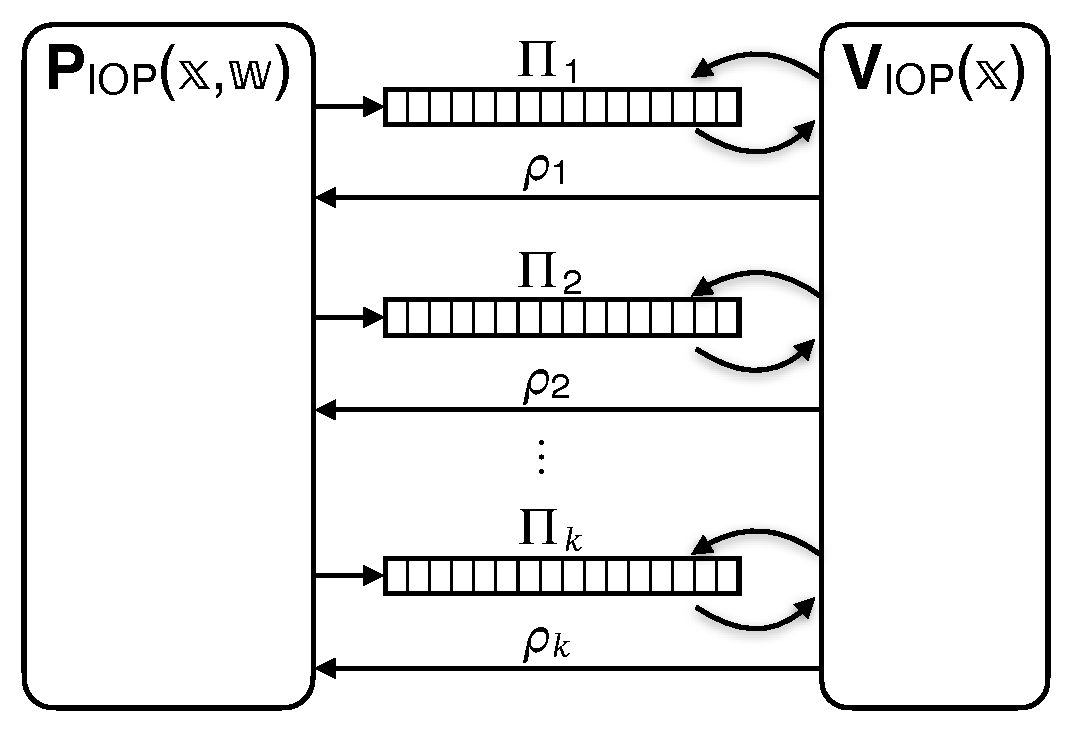
\includegraphics[width=0.6\textwidth]{\FigureFolder/iop-diagram}
\caption{Diagram of an IOP.}
\label{figure:iop-diagram}
\end{figure}

The tuple $\IOPSymbol=\IOPSystem$ is an IOP for a relation $\Relation$ with \emph{(perfect) completeness} and \emph{soundness error $\IOPSoundnessError$} if it satisfies the two properties stated below.

\begin{definition}
\label{definition:iop-completeness}
$\IOPSymbol=\IOPSystem$ for a relation $\Relation$ has \defemph{perfect completeness} if for every $(\Instance,\Witness) \in \Relation$,
\begin{equation*}
\Pr[
\IOPInteract{\IOPProver(\Instance,\Witness)}{\IOPVerifier(\Instance)}=1
]
=1
\enspace.
\end{equation*}
\end{definition}

\begin{definition}
\label{definition:iop-soundness}
$\IOPSymbol=\IOPSystem$ for a relation $\Relation$ has \defemph{soundness error $\IOPSoundnessError$} if for every $\Instance \notin \GetLanguage{\Relation}$ and malicious IOP prover $\IOPMaliciousProver$,
\begin{equation*}
\Pr[
\IOPInteract{\IOPMaliciousProver}{\IOPVerifier(\Instance)}=1
]
\leq
\IOPSoundnessError(\Instance)
\enspace.
\end{equation*}
We additionally define $\IOPSoundnessError(\InstanceSize) \DefineEqual \MaxSoundness{\IOPSoundnessError(\Instance)}$.
\end{definition}

Above, given two interactive algorithms $A$ and $B$, we use the notation $\IOPInteract{A}{B}$ to indicate the random variable that equals the output of $B$ after interacting with $A$, and where the probability is taken over any randomness used by $A$ or $B$.

\parhead{Public-coin IOPs}
We only consider IOPs that are \emph{public-coin}, which is a property of the IOP verifier $\IOPVerifier$ (and is analogous to the one for the case of IPs in \Cref{definition:ip-public-coin}).

\begin{definition}
\label{definition:iop-public-coin}
$\IOPSymbol=\IOPSystem$ is \defemph{public-coin} if every message $\IOPVerifierRandomMessage_{\RoundIndex}$ sent by the IOP verifier $\IOPVerifier$ is a random binary string of some prescribed size $\IOPRandomnessComplexity_{\RoundIndex}$ (that is statistically independent of everything else); moreover, the IOP verifier $\IOPVerifier$ has no other randomness. In this case, the decision bit of the IOP verifier $\IOPVerifier$ is a function only of the instance $\Instance$, the IOP verifier randomness $\IOPVerifierRandomMessage = \IOPVerifierRandomMessages$, and answers to queries to the received IOP strings $\IOPStrings$. We denote this bit by
\begin{equation*}
\IOPVerifier^{\IOPStrings}(\IOPVerifierInput)
\enspace.
\end{equation*}
\end{definition}

In a public-coin IOP all queries by the IOP verifier can, without loss of generality, be postponed until after the interaction with the IOP prover. This is because the IOP verifier's messages to the IOP prover do not depend on the answer to any query. Therefore, a public-coin IOP can be viewed as having two phases:
\begin{inparaenum}[(i)]
  \item the \emph{interaction phase}, where the IOP prover and IOP verifier exchange messages, and the IOP verifier does not make any queries; and then
  \item the \emph{query phase}, where the IOP verifier queries the received proof strings and then outputs a decision bit, based on the instance $\Instance$, the IOP verifier randomness $\IOPVerifierRandomMessage = \IOPVerifierRandomMessages$, and answers to its queries.
\end{inparaenum}

\parhead{Efficiency measures}
We are interested in several efficiency measures of a IOP.
\begin{itemize}

  \item \emph{Round complexity}, denoted $\IOPRoundComplexity$, is the number of back-and-forth interactions between the prover and verifier.

  \item \emph{Alphabet}, denoted $\IOPAlphabet$, is the alphabet used to write proof strings. (In general, each proof string may be over a different alphabet, or multiple alphabets, but for simplicity we focus on one alphabet for all proof strings.)

  \item \emph{Proof length}, denoted $\IOPProofLength$, is the number of symbols across all proof strings. The total number of bits across all proof strings is thus $\IOPProofLength \cdot \log \Cardinality{\IOPAlphabet}$. We denote by $\IOPProofLength_{\RoundIndex}$ the number of symbols in the proof string in round $\RoundIndex \in [\IOPRoundComplexity]$. Hence $\IOPProofLength = \sum_{\RoundIndex \in [\IOPRoundComplexity]} \IOPProofLength_{\RoundIndex}$.

  \item \emph{Randomness complexity}, denoted $\IOPRandomnessComplexity$, is the number of random bits used by the verifier across all rounds. We denote by $\IOPRandomnessComplexity_{\RoundIndex}$ the randomness complexity in round $\RoundIndex \in [\IOPRoundComplexity]$. Hence $\IOPRandomnessComplexity = \sum_{\RoundIndex \in [\IOPRoundComplexity]} \IOPRandomnessComplexity_{\RoundIndex}$.

  \item \emph{Query complexity}, denoted $\IOPQueryComplexity$, is the number of locations in all proof strings read by the verifier. (Hence each query returns a symbol of $\log \Cardinality{\IOPAlphabet}$ bits.) We denote by $\IOPQueryComplexity_{\RoundIndex}$ the query complexity to the proof string in round $\RoundIndex \in [\IOPRoundComplexity]$. Hence $\IOPQueryComplexity = \sum_{\RoundIndex \in [\IOPRoundComplexity]} \IOPQueryComplexity_{\RoundIndex}$.

  \item \emph{Prover time and verifier time}, denoted $\IOPProverTime$ and $\IOPVerifierTime$, are the time complexities of the prover (to output the IOP strings) and verifier (to output its decision bit).

\end{itemize}
The above efficiency measures may be functions of the instance $\Instance$ (and possibly other parameters associated to the construction of an IOP).

\parhead{Non-oracle messages}
In some IOP constructions it is useful to allow the IOP prover to send non-oracle messages: in each round $\RoundIndex \in [\IOPRoundComplexity]$ of an IOP, the IOP prover may send, in addition to the proof string $\IOPString_{\RoundIndex}$, a non-oracle message $\IOPProverMessage_{\RoundIndex}$ that the IOP verifier reads in its entirety. Thus, in the case of a public-coin IOP, the decision of the IOP verifier would then be computed as
\begin{equation*}
\IOPVerifier^{\IOPStrings}(\IOPVerifierInputWithProverMessages)
\enspace.
\end{equation*}
One could view the non-oracle message $\IOPProverMessage_{\RoundIndex}$ to be a segment of the IOP string $\IOPString_{\RoundIndex}$ that the IOP verifier always queries, but this view incurs minor overheads in constructions of succinct arguments based on IOPs. These overheads can be avoided via simple modifications to the construction that directly support non-oracle messages; we discuss these in \Cref{remark:ibcs-non-oracle-messages,remark:bcs-non-oracle-messages}.



\parhead{Knowledge soundness}
The soundness notion (\Cref{definition:iop-soundness}) can be strengthened to knowledge soundness notions that are analogous to those in the case of IPs in \Cref{section:ip-definitions}. Informally, whenever an IOP prover convinces the IOP verifier, then an efficient extractor finds a witness (up to some error), given suitable information about the IOP prover.

Fix any instance $\Instance$ and IOP prover $\IOPMaliciousProver$. The IOP prover $\IOPMaliciousProver$ and IOP verifier $\IOPVerifier$ (on input $\Instance$) interact; denote by $\IOPTranscript$ the transcript of this interaction and by $\DecisionBit$ the decision bit of the IOP verifier $\IOPVerifier$. The knowledge extractor $\IOPExtractor$ is tasked to find a witness $\Witness$ when given as input the instance $\Instance$, the interaction transcript $\IOPTranscript$, and black-box access to the IOP prover $\IOPMaliciousProver$. This means that the knowledge extractor $\IOPExtractor$ is \emph{rewinding}: it can re-run the IOP prover $\IOPMaliciousProver$ multiple times, possibly with correlated inputs. The knowledge soundness error is an upper bound on the probability that $\DecisionBit=1$ ($\IOPMaliciousProver$ convinces $\IOPVerifier$) and $(\Instance,\Witness) \notin \Relation$ ($\IOPExtractor$ does not find a witness). In general, the knowledge soundness error may be a function of the failure probability of $\IOPMaliciousProver$, which we define below.

\begin{definition}
\label{definition:iop-failure-probability}
Let $\IOPSymbol=\IOPSystem$ be an IOP. A deterministic IOP prover $\IOPMaliciousProver$ has \defemph{failure probability $\ProverFailureProbability{\IOPMaliciousProver}$} if for every instance $\Instance$:
\begin{equation*}
\Pr[
\IOPInteract{\IOPMaliciousProver}{\IOPVerifier(\Instance)}=0
]
\leq \ProverFailureProbability{\IOPMaliciousProver}(\Instance)
\enspace.
\end{equation*}
\end{definition}

\begin{definition}
\label{definition:iop-knowledge-soundness}
$\IOPSymbol=\IOPSystem$ for a relation $\Relation$ has \defemph{rewinding knowledge soundness error $\IOPKnowledgeError$ with extraction time $\IOPKnowledgeTime$} if there exists a probabilistic algorithm $\IOPExtractor$ (the \emph{extractor}) such that for every instance $\Instance$ and deterministic IOP prover $\IOPMaliciousProver$ with running time $\ProverRunningTime{\IOPMaliciousProver}$ the following holds:
\begin{equation*}
\Pr\left[
\begin{array}{l}
(\Instance,\Witness) \notin \Relation \\
\land\;\DecisionBit=1
\end{array}
\GivenExperiment
\StateExperiment{
\DecisionBit \xleftarrow{\IOPTranscript} \IOPInteract{\IOPMaliciousProver}{\IOPVerifier(\Instance)} \\
\Witness \gets \IOPExtractor(\Instance,\IOPTuple{\IOPString},\IOPTuple{\IOPVerifierRandomMessage},\BlackBox{\IOPMaliciousProver})
}
\right]
\leq
\IOPKnowledgeError(\Instance,\ProverFailureProbability{\IOPMaliciousProver}(\Instance))
\enspace.
\end{equation*}
Moreover, $\IOPExtractor(\Instance,\IOPTuple{\IOPString},\IOPTuple{\IOPVerifierRandomMessage},\BlackBox{\IOPMaliciousProver})$ runs in expected time $\IOPKnowledgeTime(\Instance,\ProverFailureProbability{\IOPMaliciousProver}(\Instance),\ProverRunningTime{\IOPMaliciousProver}(\Instance))$. We additionally define
\begin{align*}
\IOPKnowledgeError(\InstanceSize,\ProverFailureProbability{\IOPMaliciousProver}) &\DefineEqual \MaxKnowledge{\IOPKnowledgeError(\Instance,\ProverFailureProbability{\IOPMaliciousProver}(\Instance))}
\enspace,\quad\text{and} \\
\IOPKnowledgeTime(\InstanceSize,\ProverFailureProbability{\IOPMaliciousProver},\ProverRunningTime{\IOPMaliciousProver}) &\DefineEqual \MaxKnowledge{\IOPKnowledgeTime(\Instance,\ProverFailureProbability{\IOPMaliciousProver}(\Instance),\ProverRunningTime{\IOPMaliciousProver}(\Instance))}
\enspace.
\end{align*}
\end{definition}

If $\IOPSymbol=\IOPSystem$ has knowledge soundness error $\IOPKnowledgeError$ (with any extraction time $\IOPKnowledgeTime$) then it has soundness error $\IOPSoundnessError$ such that $\IOPSoundnessError(\Instance) \leq \min_{\ProverFailureProbability{} \in [0,1]} \IOPKnowledgeError(\Instance,\ProverFailureProbability{})$: if $\Instance \notin \GetLanguage{\Relation}$ then the extractor cannot output a witness $\Witness$ such that $(\Instance,\Witness) \in \Relation$ (as none exists), in which case the event bounded by the knowledge soundness condition equals the event bounded by the soundness condition.

A notable special case of \Cref{definition:iop-knowledge-soundness} is \emph{straightline extraction}: $\IOPExtractor$ is a polynomial-time deterministic algorithm that receives as input the instance $\Instance$ and IOP strings $\IOPTuple{\IOPString}$ (but not the IOP verifier messages $\IOPTuple{\IOPVerifierRandomMessage}$ or access to $\IOPMaliciousProver$).

\begin{definition}
\label{definition:iop-knowledge-straightline}
$\IOPSymbol=\IOPSystem$ for a relation $\Relation$ has \defemph{straightline knowledge soundness error $\IOPKnowledgeError$} if there exists a polynomial-time deterministic algorithm $\IOPExtractor$ (the \emph{extractor}) such that for every deterministic IOP prover $\IOPMaliciousProver$ and instance $\Instance$:
\begin{equation*}
\Pr\left[
\begin{array}{l}
(\Instance,\Witness) \notin \Relation \\
\land\;\DecisionBit=1
\end{array}
\GivenExperiment
\StateExperiment{
\DecisionBit \xleftarrow{\IOPTranscript} \IOPInteract{\IOPMaliciousProver}{\IOPVerifier(\Instance)} \\
\Witness \gets \IOPExtractor(\Instance,\IOPStrings)
}
\right]
\leq \IOPKnowledgeError(\Instance)
\enspace.
\end{equation*}
\end{definition}

\parhead{Zero knowledge}
A notion of zero knowledge for IOPs against honest IOP verifiers suffices for the applications that we study. Informally, zero knowledge states that the view of the verifier can be efficiently simulated by a probabilistic algorithm that only has access to the instance. In the case of a IOP the view consists of the instance, the randomness, and the query answers from the given IOP string. Honest-verifier zero knowledge then requires that the simulated view is statistically close to a view in a real execution, provided that the proved statement is true.

\begin{definition}
\label{definition:iop-view}
The IOP verifier's \defemph{view} in $\IOPSymbol=\IOPSystem$ on the instance-witness pair $(\Instance,\Witness)$, denoted $\IOPView{\IOPProver}{\IOPVerifier}{\Instance}{\Witness}$, is the random variable $\IOPSampledView$ where:
\begin{itemize}[nolistsep]
  \item $\IOPVerifierRandomMessage \in \Bits^{\IOPRandomnessComplexity}$ is a random choice of randomness for the IOP verifier $\IOPVerifier$;
  \item $(\PCPQuerySet_{\RoundIndex} \subseteq [\PCPProofLength_{\RoundIndex}])_{\RoundIndex \in [\IOPRoundComplexity]}$ and $(\PCPEntries_{\RoundIndex} \in \PCPAlphabet^{\PCPQuerySet_{\RoundIndex}})_{\RoundIndex \in [\IOPRoundComplexity]}$ are the queries and answers made across the $\IOPRoundComplexity$ IOP strings in an interaction between $\IOPProver(\Instance,\Witness)$ and $\IOPVerifier(\Instance, \IOPVerifierRandomMessage)$.
\end{itemize}
The IOP prover $\IOPProver(\Instance,\Witness)$ may use private randomness (not part of the IOP verifier's view). If the IOP is public-coin then the view shows each round's randomness: $\IOPPublicSampledView$.
\end{definition}

\begin{definition}
\label{definition:iop-hvzk}
$\IOPSymbol=\IOPSystem$ for a relation $\Relation$ has \defemph{honest-verifier zero-knowledge error $\IOPZKError$} if there exists a polynomial-time probabilistic algorithm $\IOPSimulator$ such that for every instance-witness pair $(\Instance,\Witness) \in \Relation$ the following random variables are $\IOPZKError(\Instance)$-close in statistical distance:
\begin{equation*}
\IOPView{\IOPProver}{\IOPVerifier}{\Instance}{\Witness}
\TextAndInMath
\IOPSimulator(\Instance)
\enspace.
\end{equation*}
We additionally define $\IOPZKError(\InstanceSize) \DefineEqual \MaxZK{\IOPZKError(\Instance)}$.
\end{definition}

\parhead{Verification on local views}
We sometimes run an IOP verifier with query access to \emph{partial} IOP strings defined on a subset of locations, and it is useful to introduce notation for this setting.

\begin{definition}
\label{definition:iop-local-view}
Let $(\PCPQuerySet_{\RoundIndex} \subseteq [\PCPProofLength_{\RoundIndex}])_{\RoundIndex \in [\IOPRoundComplexity]}$ be query sets, $(\PCPEntries_{\RoundIndex} \in \PCPAlphabet^{\PCPQuerySet_{\RoundIndex}})_{\RoundIndex \in [\IOPRoundComplexity]}$ query answers, $\Instance$ an instance, and $\IOPVerifierRandomMessage = \IOPVerifierRandomMessages \in \Bits^{\IOPRandomnessComplexity}$ a choice of IOP randomness (split according to rounds). We denote by
\begin{equation*}
\IOPVerifier^{\IOPLocalView{\IOPQuerySet}{\IOPEntries}}(\Instance,\IOPVerifierRandomMessages)
\end{equation*}
the decision bit of the IOP verifier $\IOPVerifier$, given instance $\Instance$ and IOP randomness $\IOPVerifierRandomMessage = \IOPVerifierRandomMessages$, when each query $\IOPQueryIndex \in \IOPQuerySet_{\RoundIndex}$ is answered with $\IOPEntries_{\RoundIndex}[\IOPQueryIndex] \in \IOPAlphabet$. (If $\IOPVerifier$ queries outside the sets $(\PCPQuerySet_{\RoundIndex})_{\RoundIndex \in [\IOPRoundComplexity]}$ then $\IOPVerifier^{\IOPLocalView{\IOPQuerySet}{\IOPEntries}}(\Instance,\IOPVerifierRandomMessages)=0$.)
\end{definition}


%%%%%%%%%%%%%%%%%%%%%%%%%%%%%%%%%%%%%%%%%%%%%%%%%%%%%%%%%%%%%%%%%%%%%%%%%%%%%%%
%%%%%%%%%%%%%%%%%%%%%%%%%%%%%%%%%%%%%%%%%%%%%%%%%%%%%%%%%%%%%%%%%%%%%%%%%%%%%%%
%%%%%%%%%%%%%%%%%%%%%%%%%%%%%%%%%%%%%%%%%%%%%%%%%%%%%%%%%%%%%%%%%%%%%%%%%%%%%%%
\section{State restoration}
\label{section:iop-state-restoration}

We state definitions for state-restoration soundness for public-coin IOPs. These definitions equal the definitions for public-coin IPs in \Cref{section:fs-sr-definition} except for straightforward syntactical changes:
\begin{itemize}[noitemsep]
  \item IP prover messages $\IPProverMessage_{\RoundIndex}$ are replaced by IOP strings $\IOPString_{\RoundIndex}$; and
  \item the IP acceptance condition $\IPVerifier\big(\IPVerifierInput\big)=1$ is replaced by the IOP acceptance condition $\IOPConvincingCondition=1$.
\end{itemize}
While the differences are minor, we state the definitions for the case of IOPs for the sake of completeness. We refer the reader to the discussion for IPs for motivation and intuition.

Note that the discussion in \Cref{section:fs-sr-comparison}, which compares the notions of standard soundness and state-restoration soundness for public-coin IPs, directly carries over to the case public-coin IOPs. In particular, the security of a non-interactive argument obtained from a given IOP via the BCS transformation is characterized by the state-restoration soundness of the IOP, as we discuss in \Cref{chapter:bcs-transformation}. Therefore, to ensure security of the BCS transformation, one must assume that the given IOP has small state-restoration soundness error.

As for IPs, small state-restoration soundness error for an IOP is implied by natural strong notions of soundness, such as special soundness (see \Cref{chapter:special-soundness}) and round-by-round soundness (see \Cref{chapter:rbr-soundness}).

\begin{definition}
\label{definition:iop-state-restoration-game}
The \defemph{IOP state-restoration game} for $\IOPSymbol=\IOPSystem$ with salt size $\SRSaltSize \in \Naturals$, functions $\SRRandomness=\IOPTuple{\SRRandomness} \in \RODistribution{(\IOPRandomnessComplexity_{\RoundIndex})_{\RoundIndex \in [\IOPRoundComplexity]}}$, and IOP state-restoration prover $\IOPMaliciousSRProver$ is defined below.
\begin{itemize}[noitemsep]
\item[] $\IOPStateRestorationGame{\SRSaltSize}{\SRRandomness}{\IOPMaliciousSRProver}$:
\begin{enumerate}[nolistsep]
  \item Repeat the following until $\IOPMaliciousSRProver$ decides to exit the loop.
  \begin{enumerate}[nolistsep]
    \item $\IOPMaliciousSRProver$ outputs $\IOPSRGameStateEntry{\RoundIndex}$, where $\Instance$ is an instance, $(\IOPString_{1},\dots,\IOPString_{\RoundIndex})$ are IOP strings, and $(\SRSaltString_{1},\dots,\SRSaltString_{\RoundIndex})$ are salt strings in $\Bits^{\SRSaltSize}$.
    \item Set $\IOPVerifierRandomMessage_{\RoundIndex} \DefineEqual \SRRandomness_{\RoundIndex}\IOPSRGameStateEntry{\RoundIndex}$.
    \item Send $\IOPVerifierRandomMessage_{\RoundIndex}$ to $\IOPMaliciousSRProver$.
  \end{enumerate}
  \item $\IOPMaliciousSRProver$ outputs $\IOPSRGameStateEntry{\IOPRoundComplexity}$, where $\Instance$ is an instance, $(\IOPString_{1},\dots,\IOPString_{\IOPRoundComplexity})$ are IOP strings, and $(\SRSaltString_{1},\dots,\SRSaltString_{\IOPRoundComplexity})$ are salt strings in $\Bits^{\SRSaltSize}$.
  \item For every $\RoundIndex \in [\IOPRoundComplexity]$, set $\IOPVerifierRandomMessage_{\RoundIndex} \DefineEqual \SRRandomness_{\RoundIndex}\IOPSRGameStateEntry{\RoundIndex}$.
  \item Output $\IOPSROutput$.
\end{enumerate}
\end{itemize}
We denote by $\SRTrace$ the list of move-response pairs of the form $(\IOPSRGameStateEntry{\RoundIndex},\IOPVerifierRandomMessage_{\RoundIndex})$ performed in the loop. We show $\SRTrace$ in an execution of the IOP state-restoration game using the following notation:
\begin{equation*}
\IOPSROutput \xleftarrow{\SRTrace} \IOPStateRestorationGame{\SRSaltSize}{\SRRandomness}{\IOPMaliciousSRProver}
\enspace.
\end{equation*}
We say that $\IOPMaliciousSRProver$ is \defemph{$\SRBudget$-move} if $\IOPMaliciousSRProver$ exits the loop after at most $\SRBudget$ iterations.
\end{definition}

\begin{definition}
\label{definition:iop-state-restoration-soundness}
$\IOPSymbol=\IOPSystem$ has \defemph{state-restoration soundness error $\IOPSRSoundnessError$} if for every salt size $\SRSaltSize \in \Naturals$, move budget $\SRBudget \in \Naturals$, $\SRBudget$-move malicious IOP state-restoration prover $\IOPMaliciousSRProver$, and instance size bound $\InstanceSize \in \Naturals$:
\begin{equation*}
\Pr\left[
\begin{array}{l}
\SomeSize{\Instance} \leq \InstanceSize \\
\land\;\Instance \notin \GetLanguage{\Relation} \\
\land\;\IOPConvincingCondition=1
\end{array}
\GivenExperiment
\StateExperiment{
\SRRandomness = \IOPTuple{\SRRandomness} \gets \RODistribution{(\IOPRandomnessComplexity_{\RoundIndex})_{\RoundIndex \in [\IOPRoundComplexity]}} \\
\LongExecution{\IOPSROutput}{\IOPStateRestorationGame{\SRSaltSize}{\SRRandomness}{\IOPMaliciousSRProver}}
}
\right]
\leq \IOPSRSoundnessError(\SRSaltSize,\SRBudget,\InstanceSize)
\enspace.
\end{equation*}
\end{definition}

\begin{definition}
\label{definition:iop-state-restoration-knowledge-straightline}
$\IOPSymbol=\IOPSystem$ has \defemph{straightline state-restoration knowledge soundness error $\IOPSRKnowledgeError$} if there exists a polynomial-time deterministic algorithm $\IOPSRExtractor$ (the \emph{extractor}) such that for every salt size $\SRSaltSize \in \Naturals$, move budget $\SRBudget \in \Naturals$, $\SRBudget$-move deterministic IOP state-restoration prover $\IOPMaliciousSRProver$, and instance size bound $\InstanceSize$:
\begin{equation*}
\Pr\left[
\begin{array}{l}
\SomeSize{\Instance} \leq \InstanceSize \\
\land\;(\Instance,\Witness) \notin \Relation \\
\land\;\IOPConvincingCondition=1
\end{array}
\GivenExperiment
\StateExperiment{
\SRRandomness = \IOPTuple{\SRRandomness} \gets \RODistribution{(\IOPRandomnessComplexity_{\RoundIndex})_{\RoundIndex \in [\IOPRoundComplexity]}} \\
\LongExecutionOver{\IOPSROutput}{\IOPStateRestorationGame{\SRSaltSize}{\SRRandomness}{\IOPMaliciousSRProver}}{\SRTrace} \\
\Witness \gets \IOPSRExtractor(\Instance,\IOPStrings,(\SRSaltString_{\RoundIndex})_{\RoundIndex \in [\IOPRoundComplexity]},\SRTrace)
}
\right]
\leq \IOPSRKnowledgeError(\SRSaltSize,\SRBudget,\InstanceSize)
\enspace.
\end{equation*}
\end{definition}

\begin{definition}
\label{definition:iop-sr-failure-probability}
Let $\IOPSymbol=\IOPSystem$ be an IOP. A deterministic IOP state-restoration prover $\IOPMaliciousSRProver$ has \defemph{failure probability $\ProverFailureProbability{\IOPMaliciousSRProver}$} if for every salt size $\SRSaltSize \in \Naturals$ and instance size bound $\InstanceSize$:
\begin{equation*}
\Pr\left[
\begin{array}{l}
\SomeSize{\Instance} > \InstanceSize \\
\lor\;\IOPConvincingCondition=0
\end{array}
\GivenExperiment
\StateExperiment{
\SRRandomness = \IOPTuple{\SRRandomness} \gets \RODistribution{(\IOPRandomnessComplexity_{\RoundIndex})_{\RoundIndex \in [\IOPRoundComplexity]}} \\
\LongExecution{\IOPSROutput}{\IOPStateRestorationGame{\SRSaltSize}{\SRRandomness}{\IOPMaliciousSRProver}} \\
}
\right]
\leq \ProverFailureProbability{\IOPMaliciousSRProver}(\SRSaltSize,\InstanceSize)
\enspace.
\end{equation*}
\end{definition}

\begin{definition}
\label{definition:iop-state-restoration-knowledge}
$\IOPSymbol=\IOPSystem$ has \defemph{rewinding state-restoration knowledge soundness error $\IOPSRKnowledgeError$ with extraction time $\IOPSRKnowledgeTime$} if there exists a probabilistic algorithm $\IOPSRExtractor$ (the \emph{extractor}) such that for every salt size $\SRSaltSize \in \Naturals$, move budget $\SRBudget \in \Naturals$, $\SRBudget$-move deterministic IOP state-restoration prover $\IOPMaliciousSRProver$ with failure probability $\ProverFailureProbability{\IOPMaliciousSRProver}$ and running time $\ProverRunningTime{\IOPMaliciousSRProver}$, and instance size bound $\InstanceSize$:
\begin{align*}
\Pr& \left[
\begin{array}{l}
\SomeSize{\Instance} \leq \InstanceSize \\
\land\;(\Instance,\Witness) \notin \Relation \\
\land\;\IOPConvincingCondition=1
\end{array}
\GivenExperiment
\StateExperiment{
\SRRandomness = \IOPTuple{\SRRandomness} \gets \RODistribution{(\IOPRandomnessComplexity_{\RoundIndex})_{\RoundIndex \in [\IOPRoundComplexity]}} \\
\LongExecutionOver{\IOPSROutput}{\IOPStateRestorationGame{\SRSaltSize}{\SRRandomness}{\IOPMaliciousSRProver}}{\SRTrace} \\
\Witness \gets \IOPSRExtractor(\Instance,\IOPStrings,(\SRSaltString_{\RoundIndex})_{\RoundIndex \in [\IOPRoundComplexity]},\IOPVerifierRandomMessages,\SRTrace,\BlackBox{\IOPMaliciousSRProver})
}
\right]
\\ & \leq \IOPSRKnowledgeError(\SRSaltSize,\SRBudget,\InstanceSize,\ProverFailureProbability{\IOPMaliciousSRProver}(\SRSaltSize,\InstanceSize))
\enspace.
\end{align*}
Moreover, $\IOPSRExtractor$ runs in expected time $\IOPSRKnowledgeTime(\SRSaltSize,\SRBudget,\InstanceSize,\ProverFailureProbability{\IOPMaliciousSRProver}(\SRSaltSize,\InstanceSize),\ProverRunningTime{\IOPMaliciousSRProver}(\SRSaltSize,\InstanceSize))$ (over the given inputs and internal randomness).
\end{definition}


%%%%%%%%%%%%%%%%%%%%%%%%%%%%%%%%%%%%%%%%%%%%%%%%%%%%%%%%%%%%%%%%%%%%%%%%%%%%%%%
%%%%%%%%%%%%%%%%%%%%%%%%%%%%%%%%%%%%%%%%%%%%%%%%%%%%%%%%%%%%%%%%%%%%%%%%%%%%%%%
%%%%%%%%%%%%%%%%%%%%%%%%%%%%%%%%%%%%%%%%%%%%%%%%%%%%%%%%%%%%%%%%%%%%%%%%%%%%%%%
%%%%%%%%%%%%%%%%%%%%%%%%%%%%%%%%%%%%%%%%%%%%%%%%%%%%%%%%%%%%%%%%%%%%%%%%%%%%%%%
\chapter{Warmup: succinct interactive arguments from IOPs}
\label{chapter:ibcs-transformation}

We describe how to construct a succinct \emph{interactive} argument, starting from any public-coin interactive oracle proof (IOP); later, in \Cref{chapter:bcs-transformation}, we describe how to additionally achieve a succinct \emph{non-interactive} argument. The non-interactive argument in \Cref{chapter:bcs-transformation} is known as the Ben-Sasson--Chiesa--Spooner (BCS) transformation, and the interactive argument in this chapter is a simplification of it known as the \emph{interactive BCS (iBCS) transformation}. Throughout, we assume familiarity with the Merkle commitment scheme as introduced in \Cref{chapter:merkle-commitment}.



%%%%%%%%%%%%%%%%%%%%%%%%%%%%%%%%%%%%%%%%%%%%%%%%%%%%%%%%%%%%%%%%%%%%%%%%%%%%%%%
%%%%%%%%%%%%%%%%%%%%%%%%%%%%%%%%%%%%%%%%%%%%%%%%%%%%%%%%%%%%%%%%%%%%%%%%%%%%%%%
%%%%%%%%%%%%%%%%%%%%%%%%%%%%%%%%%%%%%%%%%%%%%%%%%%%%%%%%%%%%%%%%%%%%%%%%%%%%%%%
\section{Construction}
\label{section:ibcs-construction}

The IOP model envisages a setting where the IOP verifier interacts with the IOP prover and has query access to the IOP prover's messages. Similarly to the Kilian transformation for PCPs (see \Cref{chapter:kilian-transformation}), the succinct interactive argument that we describe here relies on the Merkle commitment scheme to \DoQuote{implement} this query access interface. While this approach works for a more general class of IOPs, here we describe and analyze the case for public-coin IOPs.

The interactive phase of the public-coin IOP is mapped to a corresponding phase of the interactive argument: for each round $\RoundIndex \in [\IOPRoundComplexity]$, the argument prover uses the IOP prover to generate the $\RoundIndex$-th proof string $\IOPString_{\RoundIndex}$, uses the Merkle commitment scheme to generate a short commitment $\MTCommitment_{\RoundIndex}$ to $\IOPString_{\RoundIndex}$, and sends $\MTCommitment_{\RoundIndex}$ to the argument verifier; then the argument verifier sends the IOP verifier's (random) $\RoundIndex$-th message $\IOPVerifierRandomMessage_{\RoundIndex}$ to the argument prover.

Next, the query phase of the public-coin IOP is mapped to a final message: the argument prover, having now received all IOP verifier random messages, simulates the IOP verifier in order to determine its queries across all IOP strings, and then sends a message that includes the queried locations, the query answers, and Merkle opening proofs that authenticate the answers for those locations (relative to the Merkle commitments sent earlier).

Finally, the argument verifier checks that the IOP verifier accepts (given the instance, its randomness, and answers to the queries) and that all Merkle opening proofs are valid.

Note that the IOP strings $\IOPStrings$ may, in general, have different lengths $\IOPTuple{\IOPProofLength}$. Hence, for each round $\RoundIndex \in [\IOPRoundComplexity]$, we configure a Merkle commitment scheme $\MTSymbol_{\RoundIndex} \DefineEqual \MTConstructor{\SecurityParameter}{\IOPAlphabet}{\IOPProofLength_{\RoundIndex}}{\PrivacyParameter}$ to be used to commit to the $\RoundIndex$-th IOP string $\IOPString_{\RoundIndex} \in \IOPAlphabet^{\IOPProofLength_{\RoundIndex}}$. For simplicity we do not consider different random oracles across the different configurations (doing so simplifies the analysis slightly but adds more notation to the construction).

Below we describe the construction in detail.

\begin{ImportantConstruction}{\IBCSText}{ibcs-transformation}
Let $\IOPSymbol=\IOPSystem$ be a public-coin IOP with round complexity $\IOPRoundComplexity$, proof length $\IOPProofLength$ over alphabet $\IOPAlphabet$, query complexity $\IOPQueryComplexity$, and randomness complexity $\IOPRandomnessComplexity$. Let $\SecurityParameter \in \Naturals$ be a security parameter and $\PrivacyParameter \in \Naturals$ be a privacy parameter. For every $\RoundIndex \in [\IOPRoundComplexity]$, define $\MTSymbol_{\RoundIndex} \DefineEqual \MTConstructor{\SecurityParameter}{\IOPAlphabet}{\IOPProofLength_{\RoundIndex}}{\PrivacyParameter}$ to be the Merkle commitment scheme with the stated parameters. (The output size of the random oracle for every Merkle commitment scheme equals the security parameter $\SecurityParameter$.)

We define $\IARGSymbol \DefineEqual \IBCSTransformation{\IOPSymbol}{\SecurityParameter}{\PrivacyParameter}$ to be the public-coin interactive argument $\IARGSymbol = \ARGSystem$ constructed as follows. The argument prover $\ARGProver$ receives as input an instance $\Instance$ and witness $\Witness$, and the argument verifier $\ARGVerifier$ receives as input the instance $\Instance$. Both receive query access to a random oracle $\ROFunction \in \RODistribution{\SecurityParameter}$ and they interact as below.
\begin{enumerate}

\item For $\RoundIndex = 1,\dots,\IOPRoundComplexity$:
\begin{itemize}

  \item \emph{Prover message.}
  The argument prover $\ARGProver$ computes its $\RoundIndex$-th message as follows.
  \begin{enumerate}[nolistsep]
    \item Compute the $\RoundIndex$-th proof string (and auxiliary state) of the IOP prover:
    \begin{equation*}
    (\IOPString_{\RoundIndex} \in \IOPAlphabet^{\IOPProofLength_{\RoundIndex}},\IOPAuxiliaryState_{\RoundIndex})
    \DefineEqual
    \begin{cases}
    \IOPProver(\Instance,\Witness)
    & \text{ if $\RoundIndex=1$} \\
    \IOPProver(\IOPAuxiliaryState_{\RoundIndex-1},\IOPVerifierRandomMessage_{\RoundIndex-1})
    & \text{ if $\RoundIndex>1$}
    \end{cases}
    \enspace.
    \end{equation*}
    \item Commit to $\IOPString_{\RoundIndex}$ via the Merkle commitment scheme $\MTSymbol_{\RoundIndex}$:
    \begin{equation*}
    (\MTCommitment_{\RoundIndex},\MTTrapdoor_{\RoundIndex}) \DefineEqual \MTIdxCommit{\RoundIndex}^{\ROFunction}(\IOPString_{\RoundIndex})
    \enspace.
    \end{equation*}
    \item \label{step:ibcs-send-commitment}
    Send the $\RoundIndex$-th Merkle commitment $\MTCommitment_{\RoundIndex} \in \Bits^{\SecurityParameter}$.
  \end{enumerate}

  \item \emph{Verifier message.}
  The argument verifier $\ARGVerifier$ sends the $\RoundIndex$-th random message $\IOPVerifierRandomMessage_{\RoundIndex} \in \Bits^{\IOPRandomnessComplexity_{\RoundIndex}}$ for the IOP verifier $\IOPVerifier$.

\end{itemize}

\item \emph{Answer queries.}
The argument prover $\ARGProver$ does the following.
\begin{enumerate}[nolistsep]
  \item \label{step:ibcs-simulate-verifier}
  Simulate the IOP verifier $\IOPVerifier^{\IOPStrings}(\IOPVerifierInput)$, yielding query sets $(\IOPQuerySet_{\RoundIndex} \subseteq [\IOPProofLength_{\RoundIndex}])_{\RoundIndex \in [\IOPRoundComplexity]}$.
  \item For every $\RoundIndex \in [\IOPRoundComplexity]$, set $\IOPEntries_{\RoundIndex} \DefineEqual \IOPString_{\RoundIndex}[\IOPQuerySet_{\RoundIndex}] \in \IOPAlphabet^{\IOPQuerySet_{\RoundIndex}}$ to be the answers for the $\RoundIndex$-th query set.
  \item For every $\RoundIndex \in [\IOPRoundComplexity]$, compute an opening proof for $\IOPEntries_{\RoundIndex}$: $\MTProof_{\RoundIndex} \DefineEqual \MTIdxOpen{\RoundIndex}^{\ROFunction}(\MTTrapdoor_{\RoundIndex},\IOPQuerySet_{\RoundIndex})$.
  \item Send $\big((\IOPQuerySet_{\RoundIndex},\IOPEntries_{\RoundIndex},\MTProof_{\RoundIndex})\big)_{\RoundIndex \in [\IOPRoundComplexity]}$.
\end{enumerate}

\item \emph{Verification.}
The argument verifier $\ARGVerifier$ checks the following.
\begin{enumerate}[nolistsep]
  \item \label{step:ibcs-check-iop-verifier}
  Check that $\IOPVerifier^{\IOPLocalView{\IOPQuerySet}{\IOPEntries}}(\IOPVerifierInput)=1$. (The IOP verifier $\IOPVerifier(\IOPVerifierInput)$ accepts if each query $\IOPQueryIndex \in \IOPQuerySet_{\RoundIndex}$ is answered with $\IOPEntries_{\RoundIndex}[\IOPQueryIndex] \in \IOPAlphabet$. If any query falls outside the sets $(\IOPQuerySet_{\RoundIndex})_{\RoundIndex \in [\IOPRoundComplexity]}$ then reject.)
  \item Check that $\idxland{\RoundIndex \in [\IOPRoundComplexity]} \MTIdxCheck{\RoundIndex}^{\ROFunction}(\MTCommitment_{\RoundIndex},\IOPQuerySet_{\RoundIndex},\IOPEntries_{\RoundIndex},\MTProof_{\RoundIndex})=1$. (The query answers are authenticated with respect to the Merkle commitments $\IOPTuple{\MTCommitment}$.)
\end{enumerate}

\end{enumerate}
\end{ImportantConstruction}

\parhead{Efficiency}
We discuss efficiency properties of the above construction. Recall that $\IOPProofLength = \sum_{\RoundIndex \in [\IOPRoundComplexity]} \IOPProofLength_{\RoundIndex}$ and $\IOPQueryComplexity = \sum_{\RoundIndex \in [\IOPRoundComplexity]} \IOPQueryComplexity_{\RoundIndex}$, where $\IOPProofLength_{\RoundIndex}$ and $\IOPQueryComplexity_{\RoundIndex}$ are the proof length and the query complexity for the $\RoundIndex$-th proof string in the IOP, respectively.
\begin{itemize}

  \item \emph{Communication complexity.}
  The argument prover sends to the argument verifier:
\begin{itemize}[nolistsep]
  \item $\IOPRoundComplexity$ Merkle commitments, which amounts to $\IOPRoundComplexity \cdot \SecurityParameter$ bits;
  \item for each $\RoundIndex \in [\IOPRoundComplexity]$, $\IOPQueryComplexity_{\RoundIndex}$ query-answer pairs in $[\IOPProofLength_{\RoundIndex}] \times \IOPAlphabet$, which amounts to $\sum_{\RoundIndex \in [\IOPRoundComplexity]} \IOPQueryComplexity_{\RoundIndex} \cdot (\log \IOPProofLength_{\RoundIndex} + \log \Cardinality{\IOPAlphabet}) \leq \IOPQueryComplexity \cdot (\log \IOPProofLength + \log \Cardinality{\IOPAlphabet})$ bits; and
  \item for each $\RoundIndex \in [\IOPRoundComplexity]$, a Merkle opening proof for $\IOPQueryComplexity_{\RoundIndex}$ queries in $[\IOPProofLength_{\RoundIndex}]$, which amounts to $\sum_{\RoundIndex \in [\IOPRoundComplexity]} \IOPQueryComplexity_{\RoundIndex} \cdot (\PrivacyParameter + \SecurityParameter \cdot \log \IOPProofLength_{\RoundIndex}) \leq \IOPQueryComplexity \cdot (\PrivacyParameter + \SecurityParameter \cdot \log \IOPProofLength)$ bits.\footnote{See \Cref{section:compressing-opening-proof} for more on the size of Merkle opening proofs.}
\end{itemize}
Hence the number of bits sent by the argument prover is at most:
\begin{equation}
\label{equation:ibcs-prover-to-verifier}
\IOPRoundComplexity \cdot \SecurityParameter + \IOPQueryComplexity \cdot (\log \IOPProofLength + \log \Cardinality{\IOPAlphabet} + \PrivacyParameter + \SecurityParameter \cdot \log \IOPProofLength)
= O\big(\IOPRoundComplexity \cdot \SecurityParameter + \IOPQueryComplexity \cdot (\log \Cardinality{\IOPAlphabet} + \PrivacyParameter + \SecurityParameter \cdot \log \IOPProofLength)\big)
\enspace.
\end{equation}
In the other direction, the argument verifier sends to the argument prover $\IOPRandomnessComplexity = \sum_{\RoundIndex \in [\IOPRoundComplexity]} \IOPRandomnessComplexity_{\RoundIndex}$ random bits. If zero knowledge is not a goal, then the privacy parameter $\PrivacyParameter$ equals $0$.

Simply sending the (uncommitted) IOP strings $\IOPStrings$ (across an interaction) would have cost $\sum_{\RoundIndex \in [\IOPRoundComplexity]} \IOPProofLength_{\RoundIndex} \cdot \log \Cardinality{\IOPAlphabet} = \IOPProofLength \cdot \log \Cardinality{\IOPAlphabet}$ bits. Therefore, using the Merkle commitment scheme to succinctly commit and then locally open the queried locations reduces the communication complexity to $\IOPQueryComplexity \cdot (\log \IOPProofLength + \log \Cardinality{\IOPAlphabet})$ plus data used to commit and authenticate. (For most parameter settings, the precise expression mentioned above is significantly smaller than the number of bits in the IOP string.)

  \item \emph{Prover complexity.}
  The complexity of the argument prover is typically dominated by the complexity of the underlying IOP prover. Moreover, the number of queries to the random oracle is $\ARGQueryP = \sum_{\RoundIndex \in [\IOPRoundComplexity]} O(\IOPProofLength_{\RoundIndex}) = O(\IOPProofLength)$; this is because the argument prover commits to each proof string $\IOPString_{\RoundIndex} \in \IOPAlphabet^{\IOPProofLength_{\RoundIndex}}$ in $O(\IOPProofLength_{\RoundIndex})$ queries (via $\MTIdxCommit{\RoundIndex}$), and $\IOPProofLength = \sum_{\RoundIndex \in [\IOPRoundComplexity]} \IOPProofLength_{\RoundIndex}$ (this is the definition of $\IOPProofLength$).

  \item \emph{Verifier complexity.}
  The complexity of the argument verifier is typically dominated by the complexity of the underlying IOP verifier. Moreover, the number of queries to the random oracle is $\ARGQueryV = \sum_{\RoundIndex \in [\IOPRoundComplexity]} O(\IOPQueryComplexity_{\RoundIndex} \cdot \log \IOPProofLength_{\RoundIndex}) = O(\IOPQueryComplexity \cdot \log \IOPProofLength)$; this is because the argument verifier checks each opening proof $\MTProof_{\RoundIndex}$ in $O(\IOPQueryComplexity_{\RoundIndex} \cdot \log \IOPProofLength_{\RoundIndex})$ queries (via $\MTIdxCheck{\RoundIndex}$), $\IOPQueryComplexity = \sum_{\RoundIndex \in [\IOPRoundComplexity]} \IOPQueryComplexity_{\RoundIndex}$ (this is the definition of $\IOPQueryComplexity$), and $\IOPProofLength_{\RoundIndex} \leq \IOPProofLength$.

\end{itemize}

\begin{remark}[non-oracle messages in \Cref{construction:ibcs-transformation}]
\label{remark:ibcs-non-oracle-messages}
We discuss the modifications needed to additionally support non-oracle messages $\IOPTuple{\IOPProverMessage}$ from the IOP prover.
\begin{itemize}
  \item In \Cref{step:ibcs-send-commitment}, the argument prover $\ARGProver$ can additionally send a non-oracle message $\IOPProverMessage_{\RoundIndex}$ (if any is output by $\IOPProver$), in which case the $\RoundIndex$-th argument prover message is $(\MTCommitment_{\RoundIndex},\IOPProverMessage_{\RoundIndex})$.
  \item In \Cref{step:ibcs-simulate-verifier} of the argument prover $\ARGProver$, the IOP verifier is run as $\IOPVerifier^{\IOPStrings}\big(\IOPVerifierInputWithProverMessages\big)$.
  \item In \Cref{step:ibcs-check-iop-verifier} of the argument verifier $\ARGVerifier$, the explicit input to the IOP verifier is
\begin{equation*}
\big(\IOPVerifierInputWithProverMessages\big)
\enspace.
\end{equation*}
\end{itemize}
\end{remark}

\begin{figure}[htp!]
\centering
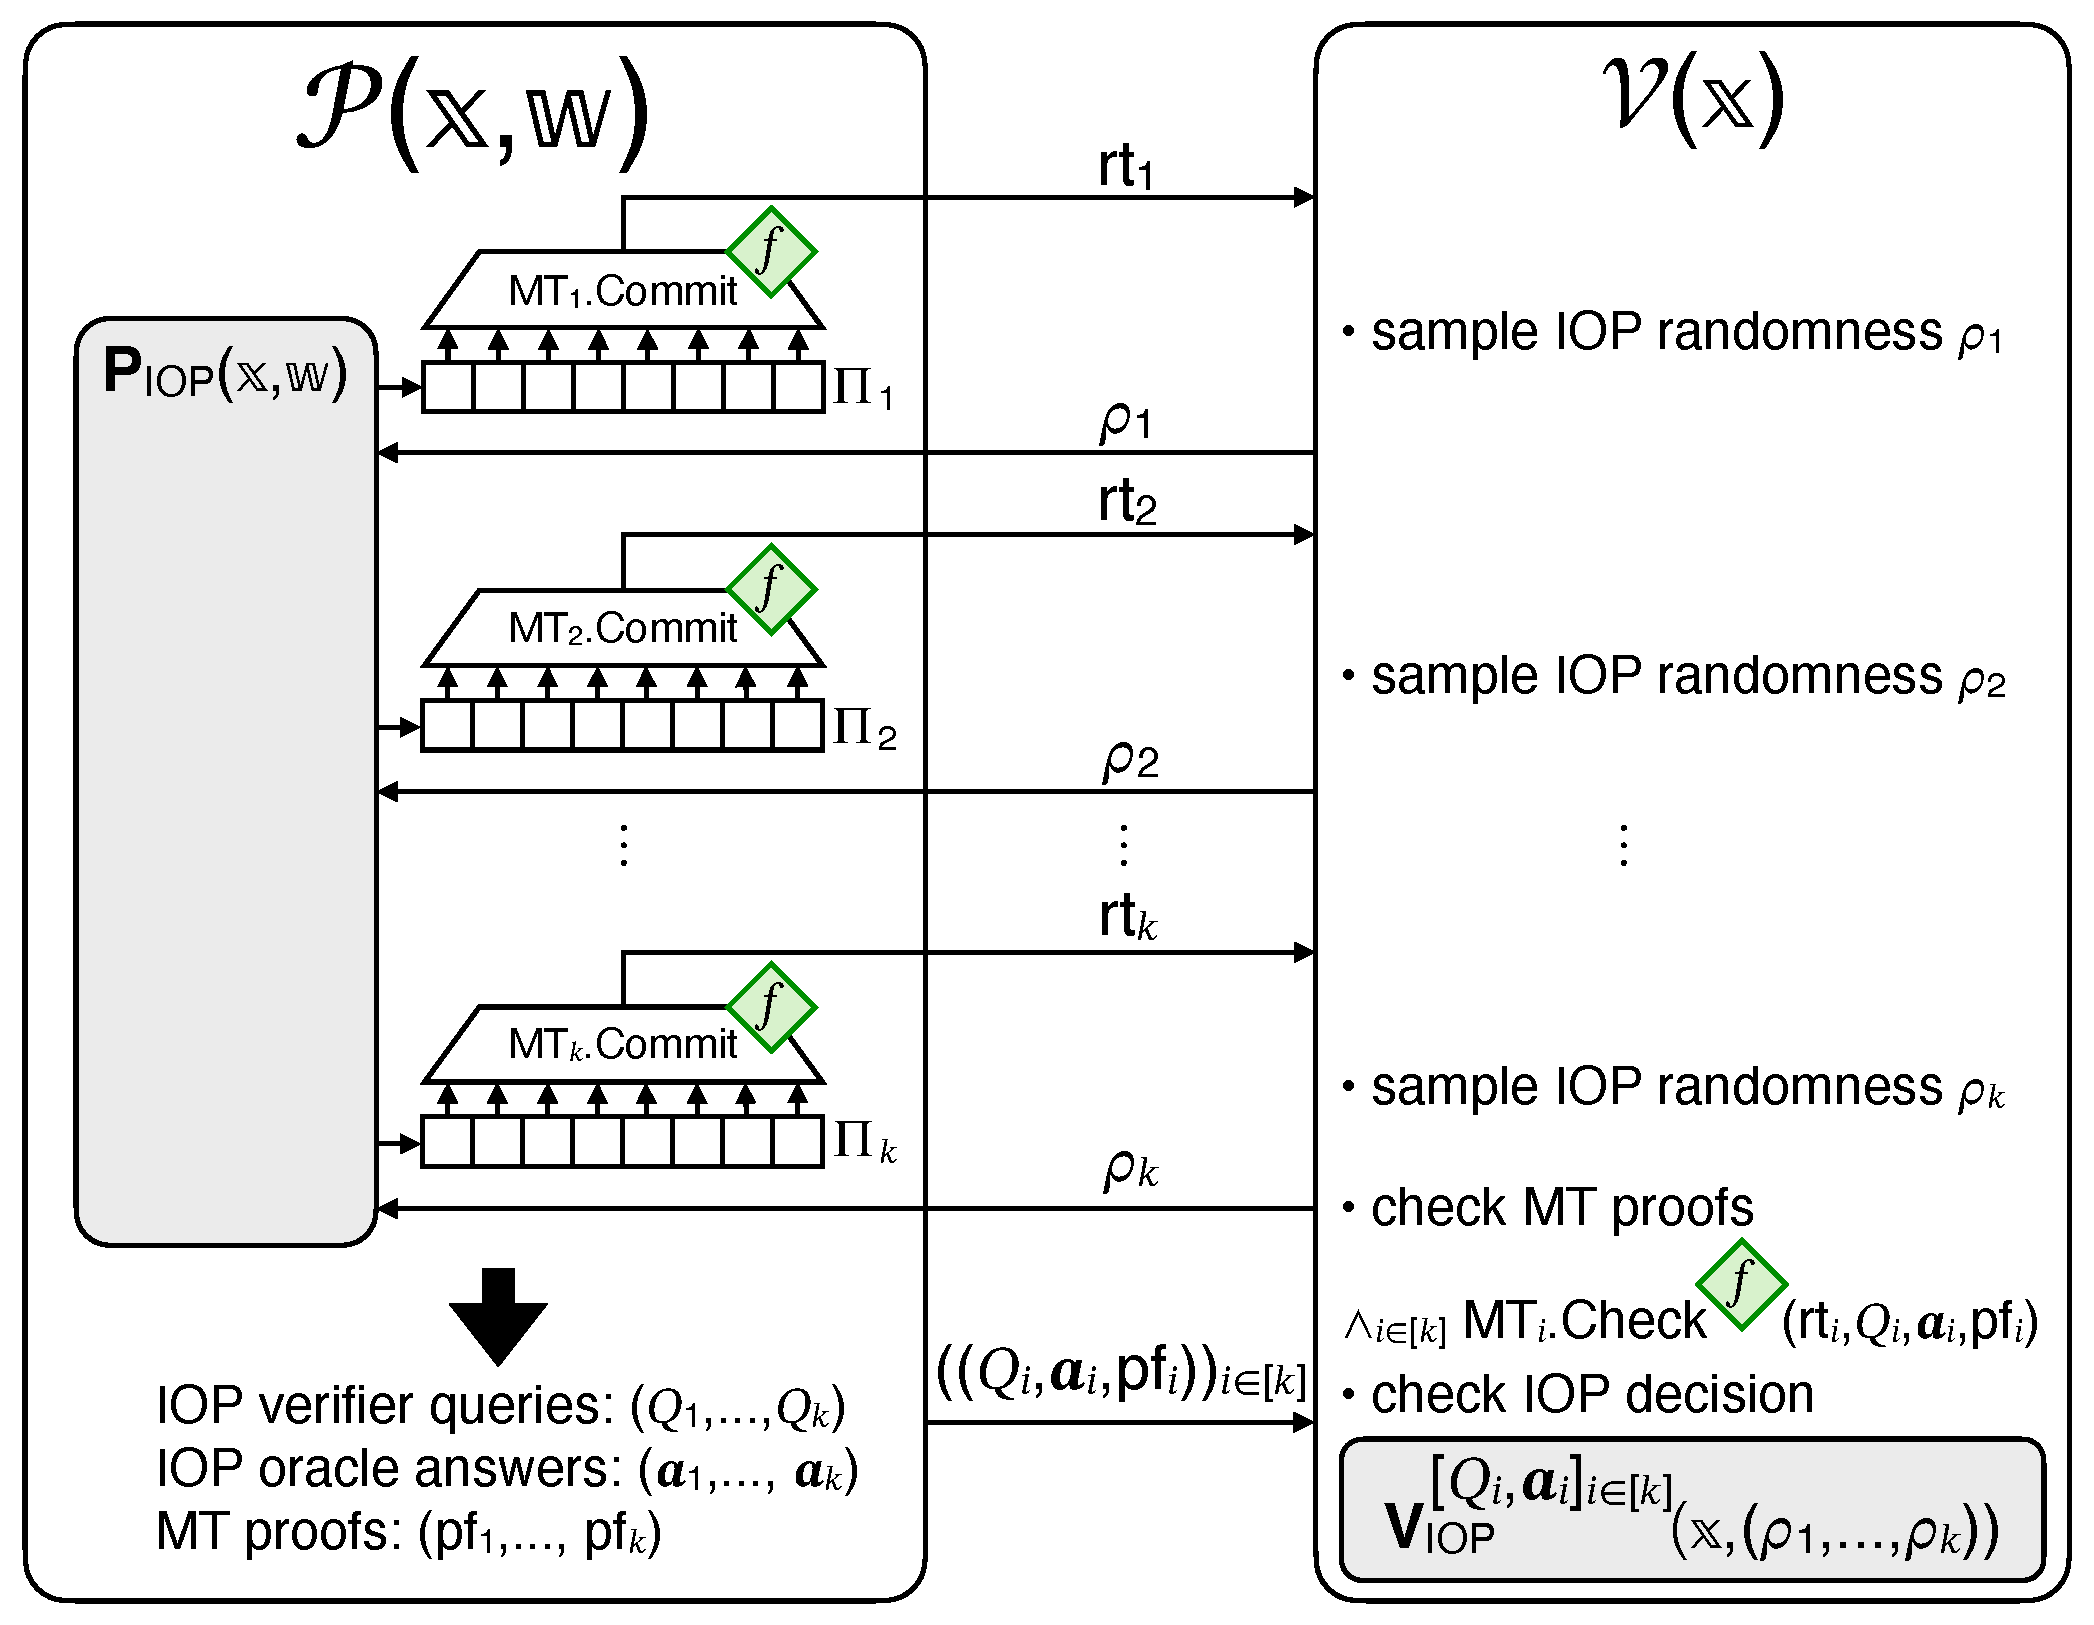
\includegraphics[width=0.8\textwidth]{\FigureFolder/ibcs-diagram}
\caption[Diagram of the iBCS transformation]{Diagram of the \IBCSText ($\IBCSSymbol$ in \Cref{construction:ibcs-transformation}).}
\label{figure:ibcs-diagram}
\end{figure}

%%%%%%%%%%%%%%%%%%%%%%%%%%%%%%%%%%%%%%%%%%%%%%%%%%%%%%%%%%%%%%%%%%%%%%%%%%%%%%%
%%%%%%%%%%%%%%%%%%%%%%%%%%%%%%%%%%%%%%%%%%%%%%%%%%%%%%%%%%%%%%%%%%%%%%%%%%%%%%%
%%%%%%%%%%%%%%%%%%%%%%%%%%%%%%%%%%%%%%%%%%%%%%%%%%%%%%%%%%%%%%%%%%%%%%%%%%%%%%%
\section{Non-adaptive soundness}
\label{section:ibcs-nonadaptive-soundness}

We prove that \Cref{construction:ibcs-transformation} is \emph{non-adaptively} sound (\Cref{definition:iarg-nonadaptive-soundness}): for any given instance that is not in the language, the probability that a bounded-query adversary convinces the argument verifier to accept is small. \Cref{theorem:ibcs-nonadaptive-soundness} below provides an upper bound on this error, which is the soundness error of the underlying IOP plus a small term. This is analogous to the case of PCPs, in \Cref{theorem:kilian-nonadaptive-soundness} (in \Cref{section:kilian-nonadaptive-soundness}). Later in \Cref{section:ibcs-adaptive-soundness} we prove that \Cref{construction:ibcs-transformation} is also \emph{adaptively} sound.

\begin{ImportantTheorem}{}{ibcs-nonadaptive-soundness}
Let $\IOPSymbol$ be a public-coin IOP for a relation $\Relation$ with soundness error $\IOPSoundnessError$, round complexity $\IOPRoundComplexity$, and proof length $\IOPProofLength$. For every security parameter $\SecurityParameter \in \Naturals$ and privacy parameter $\PrivacyParameter \in \Naturals$, $\IARGSymbol \DefineEqual \IBCSTransformation{\IOPSymbol}{\SecurityParameter}{\PrivacyParameter}$ in \Cref{construction:ibcs-transformation} is an interactive argument for $\Relation$ with non-adaptive soundness error $\ARGNASoundnessError$ (see \Cref{definition:iarg-nonadaptive-soundness}) such that
\begin{equation*}
\ARGNASoundnessError(\SecurityParameter,\ROQueryBound,\Instance)
\leq
\IOPSoundnessError(\Instance)
+
\MTMultiMultiExtractionError(\SecurityParameter,\ROQueryBound,\IOPProofLength,\IOPRoundComplexity,\IOPRoundComplexity)
\enspace.
\end{equation*}
Above $\MTMultiMultiExtractionError$ is the Merkle commitment multi-extraction error from \Cref{lemma:mt-multi-configuration-multi-extractability}, and $\MTMultiMultiExtractionError(\SecurityParameter,\ROQueryBound,\IOPProofLength,\IOPRoundComplexity,\IOPRoundComplexity) \leq \MTMultiMultiExtractabilityShortExpression{\SecurityParameter}{\ROQueryBound}$ if $\MTMultiMultiExtractabilityCondition{\ROQueryBound}{\IOPRoundComplexity}{\log\IOPProofLength}$.
\end{ImportantTheorem}

We prove the theorem via a security reduction of the following form. For every fixed instance $\Instance$, any malicious argument prover $\Malicious{\ARGProver}$ that convinces the argument verifier $\ARGVerifier(\Instance)$ with probability $\delta$ can be transformed into a corresponding malicious IOP prover $\IOPMaliciousProver$ that convinces the IOP verifier $\IOPVerifier(\Instance)$ with probability at least $\delta$ minus a small term. \Cref{theorem:ibcs-nonadaptive-soundness} follows by noting that if $\Instance \notin \GetLanguage{\Relation}$ then any IOP prover $\IOPMaliciousProver$ convinces $\IOPVerifier(\Instance)$ with probability at most $\IOPSoundnessError(\Instance)$.

Below we state the security reduction and then prove it.

\begin{lemma}
\label{lemma:ibcs-reduction}
There exists an IOP prover $\IOPMaliciousProver$ such that for every $\ROQueryBound$-query argument prover $\Malicious{\ARGProver}$ the following holds for every instance $\Instance$:
\begin{equation*}
\Pr
\left[
\ARGInteract{\Malicious{\ARGProver}^{\ROFunction}}{\ARGVerifier^{\ROFunction}(\Instance)}=1
\GivenExperiment
\StateExperiment{
\ROFunction \gets \RODistribution{\SecurityParameter}
}
\right]
\leq
\Pr
\left[
\IOPInteract{\IOPMaliciousProver(\BlackBox{\ARGProver})}{\IOPVerifier(\Instance)}=1
\right]
+
\MTMultiMultiExtractionError(\SecurityParameter,\ROQueryBound,\IOPProofLength,\IOPRoundComplexity,\IOPRoundComplexity)
\enspace.
\end{equation*}
Moreover, the running time of $\IOPMaliciousProver$ equals the running time of $\Malicious{\ARGProver}$ plus $\MTMultiMultiExtractorTimeFunction{\SecurityParameter}{\IOPAlphabet}{\IOPProofLength}{\PrivacyParameter}{\ROQueryBound}{\IOPRoundComplexity}$ where $\MTMultiMultiExtractorTimeSymbol$ is the time complexity of the Merkle commitment multi-extractor in \Cref{lemma:mt-multi-configuration-multi-extractability}.
\end{lemma}

\begin{proof}
Let $\MTMultiExtractor$ be the Merkle commitment multi-extractor for $(\MTSymbol_{\RoundIndex})_{\RoundIndex \in [\IOPRoundComplexity]}$ from \Cref{lemma:mt-multi-configuration-multi-extractability} in \Cref{section:merkle-commitment-multi-extractability}. The IOP prover $\IOPMaliciousProver$ uses the argument prover $\Malicious{\ARGProver}$ as a black box, and works as follows.
\begin{itemize}[noitemsep]
\item[] $\IOPMaliciousProver(\BlackBox{\ARGProver})$:
\begin{enumerate}[nolistsep]

  \item Start running the argument prover $\Malicious{\ARGProver}$, simulating its random oracle $\ROFunction$.

  \item For $\RoundIndex = 1,\dots,\IOPRoundComplexity$:
  \begin{enumerate}

    \item When $\Malicious{\ARGProver}$ outputs the $\RoundIndex$-th Merkle commitment $\MTCommitment_{\RoundIndex}$, let $\ROTrace_{\RoundIndex}$ be the query-answer trace of this partial execution since outputting $\MTCommitment_{\RoundIndex-1}$ (or the beginning if $\RoundIndex=1$).

    \item Run the Merkle commitment multi-extractor to obtain a proof string:
    \begin{equation*}
    (\IOPString_{\RoundIndex},\MTTrapdoor_{\RoundIndex}) \gets \MTMultiExtractor(\RoundIndex,\MTCommitment_{\RoundIndex},\ROTrace_{\RoundIndex})
    \enspace.
    \end{equation*}
    ($\MTMultiExtractor$ also outputs an opening trapdoor $\MTTrapdoor_{\RoundIndex}$, but it is not used here.)

    \item Send the IOP string $\IOPString_{\RoundIndex}$ to the IOP verifier.

    \item Receive the IOP random message $\IOPVerifierRandomMessage_{\RoundIndex} \in \Bits^{\IOPRandomnessComplexity_{\RoundIndex}}$, and forward it to $\Malicious{\ARGProver}$.

  \end{enumerate}
\end{enumerate}
\end{itemize}
The running time of $\IOPMaliciousProver$ is the running time of (a partial execution of) $\Malicious{\ARGProver}$ plus $\MTMultiMultiExtractorTimeFunction{\SecurityParameter}{\IOPAlphabet}{\IOPProofLength}{\PrivacyParameter}{\ROQueryBound}{\IOPRoundComplexity}$; indeed, the Merkle commitment multi-extractor $\MTMultiExtractor$ is invoked against an adversary that makes at most $\ROQueryBound$ queries to the random oracle and outputs $\IOPRoundComplexity$ Merkle commitments across its execution.

We now argue that the IOP prover $\IOPMaliciousProver$ satisfies the claimed property.

By construction, the argument verifier $\ARGVerifier$ accepts if and only if the IOP verifier $\IOPVerifier$ accepts and each invocation of the Merkle commitment checking algorithm $\MTIdxCheck{\RoundIndex}$ accepts:
\begin{align*}
&\Pr
\left[
\ARGInteract{\Malicious{\ARGProver}^{\ROFunction}}{\ARGVerifier^{\ROFunction}(\Instance)}=1
\GivenExperiment
\StateExperiment{
\ROFunction \gets \RODistribution{\SecurityParameter}
}
\right]
\\
=&
\Pr
\left[
\begin{array}{l}
\IOPVerifier^{\IOPLocalView{\IOPQuerySet}{\IOPEntries}}(\IOPVerifierInput)=1 \\
\land\;\idxland{\RoundIndex \in [\IOPRoundComplexity]} \MTIdxCheck{\RoundIndex}^{\ROFunction}(\MTCommitment_{\RoundIndex},\IOPQuerySet_{\RoundIndex},\IOPEntries_{\RoundIndex},\MTProof_{\RoundIndex})=1
\end{array}
\GivenExperiment
\StateExperiment{
\ROFunction \gets \RODistribution{\SecurityParameter} \\
\text{For $\RoundIndex=1,\dots,\IOPRoundComplexity$:} \\
\IndentedBullet(\MTCommitment_{\RoundIndex},\ROAdvState_{\RoundIndex}) \gets \Malicious{\ARGProver}^{\ROFunction}(\ROAdvState_{\RoundIndex-1},\IOPVerifierRandomMessage_{\RoundIndex-1}) \\
\IndentedBullet\IOPVerifierRandomMessage_{\RoundIndex} \gets \Bits^{\IOPRandomnessComplexity_{\RoundIndex}} \\
\big((\IOPQuerySet_{\RoundIndex},\IOPEntries_{\RoundIndex},\MTProof_{\RoundIndex})\big)_{\RoundIndex \in [\IOPRoundComplexity]} \gets \Malicious{\ARGProver}^{\ROFunction}(\ROAdvState_{\IOPRoundComplexity},\IOPVerifierRandomMessage_{\IOPRoundComplexity})
}
\right]
\enspace.
\end{align*}
We split the above probability as a sum of two probabilities that separately consider the disjoint cases where all extractions succeed or at least one extraction fails:
\begin{align}
\label{equation:ibcs-nonadaptive-soundess-ext-works}
&\Pr
\left[
\begin{array}{l}
\IOPVerifier^{\IOPLocalView{\IOPQuerySet}{\IOPEntries}}(\IOPVerifierInput)=1 \\
\land\;\idxland{\RoundIndex \in [\IOPRoundComplexity]} \MTIdxCheck{\RoundIndex}^{\ROFunction}(\MTCommitment_{\RoundIndex},\IOPQuerySet_{\RoundIndex},\IOPEntries_{\RoundIndex},\MTProof_{\RoundIndex})=1 \\
\land\;\idxland{\RoundIndex \in [\IOPRoundComplexity]} \IOPString_{\RoundIndex}[\IOPQuerySet_{\RoundIndex}] = \IOPEntries_{\RoundIndex}
\end{array}
\GivenExperiment
\StateExperiment{
\ROFunction \gets \RODistribution{\SecurityParameter} \\
\text{For $\RoundIndex=1,\dots,\IOPRoundComplexity$:} \\
\IndentedBullet\ROInputOutputAndTrace{\ROFunction}{\Malicious{\ARGProver}}{\ROAdvState_{\RoundIndex-1},\IOPVerifierRandomMessage_{\RoundIndex-1}}{\ROTrace_{\RoundIndex}}{(\MTCommitment_{\RoundIndex},\ROAdvState_{\RoundIndex})} \\
\IndentedBullet(\IOPString_{\RoundIndex},\MTTrapdoor_{\RoundIndex}) \gets \MTMultiExtractor(\RoundIndex,\MTCommitment_{\RoundIndex},\ROTrace_{\RoundIndex}) \\
\IndentedBullet\IOPVerifierRandomMessage_{\RoundIndex} \gets \Bits^{\IOPRandomnessComplexity_{\RoundIndex}} \\
\big((\IOPQuerySet_{\RoundIndex},\IOPEntries_{\RoundIndex},\MTProof_{\RoundIndex})\big)_{\RoundIndex \in [\IOPRoundComplexity]} \gets \Malicious{\ARGProver}^{\ROFunction}(\ROAdvState_{\IOPRoundComplexity},\IOPVerifierRandomMessage_{\IOPRoundComplexity})
}
\right] \\
\label{equation:ibcs-nonadaptive-soundess-ext-fails}
+&
\Pr
\left[
\begin{array}{l}
\IOPVerifier^{\IOPLocalView{\IOPQuerySet}{\IOPEntries}}(\IOPVerifierInput)=1 \\
\land\;\idxland{\RoundIndex \in [\IOPRoundComplexity]} \MTIdxCheck{\RoundIndex}^{\ROFunction}(\MTCommitment_{\RoundIndex},\IOPQuerySet_{\RoundIndex},\IOPEntries_{\RoundIndex},\MTProof_{\RoundIndex})=1 \\
\land\;\idxlor{\RoundIndex \in [\IOPRoundComplexity]} \IOPString_{\RoundIndex}[\IOPQuerySet_{\RoundIndex}] \neq \IOPEntries_{\RoundIndex}
\end{array}
\GivenExperiment
\StateExperiment{
\ROFunction \gets \RODistribution{\SecurityParameter} \\
\text{For $\RoundIndex=1,\dots,\IOPRoundComplexity$:} \\
\IndentedBullet\ROInputOutputAndTrace{\ROFunction}{\Malicious{\ARGProver}}{\ROAdvState_{\RoundIndex-1},\IOPVerifierRandomMessage_{\RoundIndex-1}}{\ROTrace_{\RoundIndex}}{(\MTCommitment_{\RoundIndex},\ROAdvState_{\RoundIndex})} \\
\IndentedBullet(\IOPString_{\RoundIndex},\MTTrapdoor_{\RoundIndex}) \gets \MTMultiExtractor(\RoundIndex,\MTCommitment_{\RoundIndex},\ROTrace_{\RoundIndex}) \\
\IndentedBullet\IOPVerifierRandomMessage_{\RoundIndex} \gets \Bits^{\IOPRandomnessComplexity_{\RoundIndex}} \\
\big((\IOPQuerySet_{\RoundIndex},\IOPEntries_{\RoundIndex},\MTProof_{\RoundIndex})\big)_{\RoundIndex \in [\IOPRoundComplexity]} \gets \Malicious{\ARGProver}^{\ROFunction}(\ROAdvState_{\IOPRoundComplexity},\IOPVerifierRandomMessage_{\IOPRoundComplexity})
}
\right]
\enspace.
\end{align}
We conclude the proof by upper bounding each of the two terms.
\begin{itemize}

  \item The term in \Cref{equation:ibcs-nonadaptive-soundess-ext-works} is upper bounded by the IOP error, as we now explain. If $\idxland{\RoundIndex \in [\IOPRoundComplexity]} \IOPString_{\RoundIndex}[\IOPQuerySet_{\RoundIndex}] = \IOPEntries_{\RoundIndex}$ (every extracted IOP string agrees with the relevant query answers) then $\IOPVerifier^{\IOPLocalView{\IOPQuerySet}{\IOPEntries}}(\IOPVerifierInput) = \IOPVerifier^{(\IOPString)_{\RoundIndex \in [\IOPRoundComplexity]}}(\IOPVerifierInput)$ (the IOP verifier returns the same output). Moreover, the probability does not decrease if we omit the conditions for every $\MTIdxCheck{\RoundIndex}$ (and thus can ignore the final output of $\Malicious{\ARGProver}$). Therefore the term in \Cref{equation:ibcs-nonadaptive-soundess-ext-works} can be upper bounded by the following expression:
\begin{equation*}
\Pr
\left[
\IOPVerifier^{(\IOPString)_{\RoundIndex \in [\IOPRoundComplexity]}}(\IOPVerifierInput)=1
\GivenExperiment
\StateExperiment{
\ROFunction \gets \RODistribution{\SecurityParameter} \\
\text{For $\RoundIndex=1,\dots,\IOPRoundComplexity$:} \\
\IndentedBullet\ROInputOutputAndTrace{\ROFunction}{\Malicious{\ARGProver}}{\ROAdvState_{\RoundIndex-1},\IOPVerifierRandomMessage_{\RoundIndex-1}}{\ROTrace_{\RoundIndex}}{(\MTCommitment_{\RoundIndex},\ROAdvState_{\RoundIndex})} \\
\IndentedBullet(\IOPString_{\RoundIndex},\MTTrapdoor_{\RoundIndex}) \gets \MTMultiExtractor(\RoundIndex,\MTCommitment_{\RoundIndex},\ROTrace_{\RoundIndex}) \\
\IndentedBullet\IOPVerifierRandomMessage_{\RoundIndex} \gets \Bits^{\IOPRandomnessComplexity_{\RoundIndex}}
}
\right]
\enspace.
\end{equation*}
The right-side experiment corresponds to an interaction between the IOP prover $\IOPMaliciousProver(\BlackBox{\ARGProver})$ and the IOP verifier (which sends $\IOPVerifierRandomMessage_{\RoundIndex}$ in round $\RoundIndex$). Hence the above probability equals the following probability:
\begin{equation*}
\Pr
\left[
\IOPInteract{\IOPMaliciousProver}{\IOPVerifier(\IOPVerifierInput)}=1
\GivenExperiment
\StateExperiment{
\IOPVerifierRandomMessages \gets \Bits^{\IOPRandomnessComplexity}
}
\right]
\enspace.
\end{equation*}


  \item The term in \Cref{equation:ibcs-nonadaptive-soundess-ext-fails} is upper bounded via the Merkle commitment multi-extraction error (\Cref{lemma:mt-multi-configuration-multi-extractability}), as we now explain. The probability does not decrease if we omit the condition on $\IOPVerifier$. Therefore the term in \Cref{equation:ibcs-nonadaptive-soundess-ext-fails} can be upper bounded by the following expression:
\begin{equation*}
\Pr\left[
\begin{array}{l}
\idxland{\RoundIndex \in [\IOPRoundComplexity]} \MTIdxCheck{\RoundIndex}^{\ROFunction}(\MTCommitment_{\RoundIndex},\IOPQuerySet_{\RoundIndex},\IOPEntries_{\RoundIndex},\MTProof_{\RoundIndex})=1 \\
\land\;\idxlor{\RoundIndex \in [\IOPRoundComplexity]} \IOPString_{\RoundIndex}[\IOPQuerySet_{\RoundIndex}] \neq \IOPEntries_{\RoundIndex}
\end{array}
\GivenExperiment
\StateExperiment{
\ROFunction \gets \RODistribution{\SecurityParameter} \\
\text{For $\RoundIndex=1,\dots,\IOPRoundComplexity$:} \\
\IndentedBullet\ROInputOutputAndTrace{\ROFunction}{\Malicious{\ARGProver}}{\ROAdvState_{\RoundIndex-1},\IOPVerifierRandomMessage_{\RoundIndex-1}}{\ROTrace_{\RoundIndex}}{(\MTCommitment_{\RoundIndex},\ROAdvState_{\RoundIndex})} \\
\IndentedBullet(\IOPString_{\RoundIndex},\MTTrapdoor_{\RoundIndex}) \gets \MTMultiExtractor(\RoundIndex,\MTCommitment_{\RoundIndex},\ROTrace_{\RoundIndex}) \\
\IndentedBullet\IOPVerifierRandomMessage_{\RoundIndex} \gets \Bits^{\IOPRandomnessComplexity_{\RoundIndex}} \\
\big((\IOPQuerySet_{\RoundIndex},\IOPEntries_{\RoundIndex},\MTProof_{\RoundIndex})\big)_{\RoundIndex \in [\IOPRoundComplexity]} \gets \Malicious{\ARGProver}^{\ROFunction}(\ROAdvState_{\IOPRoundComplexity},\IOPVerifierRandomMessage_{\IOPRoundComplexity})
}
\right]
\enspace.
\end{equation*}
In turn, the above probability is at most $\MTMultiMultiExtractionError(\SecurityParameter,\ROQueryBound,\IOPProofLength,\IOPRoundComplexity,\IOPRoundComplexity)$ by \Cref{lemma:mt-multi-configuration-multi-extractability}. (Here we do not use the fact that \Cref{lemma:mt-multi-configuration-multi-extractability} guarantees that each $\MTTrapdoor_{\RoundIndex}$ can be used to extract a corresponding Merkle opening proof.)

\end{itemize}
\end{proof}

%%%%%%%%%%%%%%%%%%%%%%%%%%%%%%%%%%%%%%%%%%%%%%%%%%%%%%%%%%%%%%%%%%%%%%%%%%%%%%%
%%%%%%%%%%%%%%%%%%%%%%%%%%%%%%%%%%%%%%%%%%%%%%%%%%%%%%%%%%%%%%%%%%%%%%%%%%%%%%%
%%%%%%%%%%%%%%%%%%%%%%%%%%%%%%%%%%%%%%%%%%%%%%%%%%%%%%%%%%%%%%%%%%%%%%%%%%%%%%%
\section{Adaptive soundness}
\label{section:ibcs-adaptive-soundness}

We prove that \Cref{construction:ibcs-transformation} is \emph{adaptively} sound (\Cref{definition:iarg-adaptive-soundness}): the probability that a bounded-query adversary outputs an instance not in the language and convinces the argument verifier is small. \Cref{theorem:ibcs-adaptive-soundness} below provides an upper bound on this error (which happens to be the same as the non-adaptive case in \Cref{theorem:ibcs-nonadaptive-soundness}).

\begin{ImportantTheorem}{}{ibcs-adaptive-soundness}
Let $\IOPSymbol$ be a public-coin IOP for a relation $\Relation$ with soundness error $\IOPSoundnessError$, round complexity $\IOPRoundComplexity$, and proof length $\IOPProofLength$. For every security parameter $\SecurityParameter \in \Naturals$ and privacy parameter $\PrivacyParameter \in \Naturals$, $\IARGSymbol \DefineEqual \IBCSTransformation{\IOPSymbol}{\SecurityParameter}{\PrivacyParameter}$ in \Cref{construction:ibcs-transformation} is an interactive argument for $\Relation$ with adaptive soundness error $\ARGSoundnessError$ (see \Cref{definition:iarg-adaptive-soundness}) such that
\begin{equation*}
\ARGSoundnessError(\SecurityParameter,\ROQueryBound,\InstanceSize)
\leq
\IBCSSoundnessErrorExpression
\enspace.
\end{equation*}
Above $\MTMultiMultiExtractionError$ is the Merkle commitment multi-extraction error from \Cref{lemma:mt-multi-configuration-multi-extractability}, and $\MTMultiMultiExtractionError(\SecurityParameter,\ROQueryBound,\IOPProofLength,\IOPRoundComplexity,\IOPRoundComplexity) \leq \MTMultiMultiExtractabilityShortExpression{\SecurityParameter}{\ROQueryBound}$ if $\MTMultiMultiExtractabilityCondition{\ROQueryBound}{\IOPRoundComplexity}{\log\IOPProofLength}$.
\end{ImportantTheorem}

We cannot use the security reduction in \Cref{lemma:ibcs-reduction} to prove the adaptive case, because now the choice of instance by the malicious argument prover depends on the random oracle. Nevertheless, we can adapt the statement of the lemma and its proof in a straightforward way to accommodate instances chosen by the malicious argument prover. \Cref{theorem:ibcs-adaptive-soundness} follows by noting that, for every instance $\Instance$ such that $\SomeSize{\Instance} \leq \InstanceSize$ and $\Instance \notin \GetLanguage{\Relation}$, the IOP verifier accepts $\Instance$ with probability at most $\IOPSoundnessError(\InstanceSize) = \MaxSoundness{\IOPSoundnessError(\Instance)}$ (see \Cref{definition:iop-soundness}).

\begin{lemma}
\label{lemma:ibcs-adaptive-reduction}
There exists an IOP prover $\IOPMaliciousProver$ such that for every $\ROQueryBound$-query argument prover $\Malicious{\ARGProver}$ the following holds for every instance size bound $\InstanceSize \in \Naturals$:
\begin{align*}
&\Pr
\left[
\begin{array}{l}
\SomeSize{\Instance} \leq \InstanceSize \\
\land\;\Instance \notin \GetLanguage{\Relation} \\
\land\;\ARGInteract{\Malicious{\ARGProver}^{\ROFunction}(\ROAdvState)}{\ARGVerifier^{\ROFunction}(\Instance)}=1
\end{array}
\GivenExperiment
\StateExperiment{
\ROFunction \gets \RODistribution{\SecurityParameter} \\
(\Instance,\ROAdvState) \gets \Malicious{\ARGProver}^{\ROFunction}
}
\right]
\\
&\leq
\Pr
\left[
\begin{array}{l}
\SomeSize{\Instance} \leq \InstanceSize \\
\land\;\Instance \notin \GetLanguage{\Relation} \\
\land\;\IOPInteract{\IOPMaliciousProver(\IOPAuxiliaryState,\BlackBox{\ARGProver})}{\IOPVerifier(\Instance)}=1
\end{array}
\GivenExperiment
\StateExperiment{
(\Instance,\IOPAuxiliaryState) \gets \IOPMaliciousProver(\BlackBox{\ARGProver})
}
\right]
+
\MTMultiMultiExtractionError(\SecurityParameter,\ROQueryBound,\IOPProofLength,\IOPRoundComplexity,\IOPRoundComplexity)
\enspace.
\end{align*}
Moreover, the running time of $\IOPMaliciousProver$ equals the running time of $\Malicious{\ARGProver}$ plus $\MTMultiMultiExtractorTimeFunction{\SecurityParameter}{\IOPAlphabet}{\IOPProofLength}{\PrivacyParameter}{\ROQueryBound}{\IOPRoundComplexity}$ where $\MTMultiMultiExtractorTimeSymbol$ is the time complexity of the Merkle commitment multi-extractor in \Cref{lemma:mt-multi-configuration-multi-extractability}.
\end{lemma}

\begin{proof}
Below, since the argument prover $\Malicious{\ARGProver}$ moves first, we can write that $\Malicious{\ARGProver}$ outputs simultaneously the choice of instance $\Instance$, its first message $\MTCommitment_{1}$ for $\ARGVerifier$, and an auxiliary state $\ROAdvState_{1}$ for after receiving $\ARGVerifier$'s first message.

Let $\MTMultiExtractor$ be the Merkle commitment multi-extractor for $(\MTSymbol_{\RoundIndex})_{\RoundIndex \in [\IOPRoundComplexity]}$ from \Cref{lemma:mt-multi-configuration-multi-extractability} in \Cref{section:merkle-commitment-multi-extractability}. The IOP prover $\IOPMaliciousProver$ uses the argument prover $\Malicious{\ARGProver}$ as a black box, and works as follows.
\begin{itemize}[noitemsep]
\item[] $\IOPMaliciousProver(\BlackBox{\ARGProver})$:
\begin{enumerate}[nolistsep]

  \item Start running the argument prover $\Malicious{\ARGProver}$, simulating its random oracle $\ROFunction$.

  \item For $\RoundIndex = 1,\dots,\IOPRoundComplexity$:
  \begin{enumerate}

    \item If $\RoundIndex=1$: When $\Malicious{\ARGProver}$ outputs the instance $\Instance$ and its first Merkle commitment $\MTCommitment_{1}$, let $\ROTrace_{1}$ be the query-answer trace of this partial execution since the beginning. \\ If $\RoundIndex>1$: When $\Malicious{\ARGProver}$ outputs the $\RoundIndex$-th Merkle commitment $\MTCommitment_{\RoundIndex}$, let $\ROTrace_{\RoundIndex}$ be the query-answer trace of this partial execution since outputting $\MTCommitment_{\RoundIndex-1}$.

    \item Run the Merkle commitment multi-extractor to obtain a proof string:
    \begin{equation*}
    (\IOPString_{\RoundIndex},\MTTrapdoor_{\RoundIndex}) \gets \MTMultiExtractor(\MTCommitment_{\RoundIndex},\ROTrace_{\RoundIndex})
    \enspace.
    \end{equation*}
    ($\MTMultiExtractor$ also outputs an opening trapdoor $\MTTrapdoor_{\RoundIndex}$, but it is not used here.)

    \item Send the IOP string $\IOPString_{\RoundIndex}$ to the IOP verifier.

    \item Receive the IOP random message $\IOPVerifierRandomMessage_{\RoundIndex} \in \Bits^{\IOPRandomnessComplexity_{\RoundIndex}}$, and forward it to $\Malicious{\ARGProver}$.

  \end{enumerate}
\end{enumerate}
\end{itemize}
The running time of $\IOPMaliciousProver$ is the running time of (a partial execution of) $\Malicious{\ARGProver}$ plus $\MTMultiMultiExtractorTimeFunction{\SecurityParameter}{\IOPAlphabet}{\IOPProofLength}{\PrivacyParameter}{\ROQueryBound}{\IOPRoundComplexity}$; indeed, the Merkle commitment multi-extractor $\MTMultiExtractor$ is invoked against an adversary that makes at most $\ROQueryBound$ queries to the random oracle and outputs $\IOPRoundComplexity$ Merkle commitments across its execution.

We argue that the IOP prover $\IOPMaliciousProver$ satisfies the claimed property.

By construction, the argument verifier $\ARGVerifier$ accepts if and only if the IOP verifier $\IOPVerifier$ accepts and each invocation of the Merkle commitment checking algorithm $\MTIdxCheck{\RoundIndex}$ accepts:
\begin{align*}
&\Pr
\left[
\begin{array}{l}
\SomeSize{\Instance} \leq \InstanceSize \\
\land\;\Instance \notin \GetLanguage{\Relation} \\
\land\;\ARGInteract{\Malicious{\ARGProver}^{\ROFunction}(\ROAdvState)}{\ARGVerifier^{\ROFunction}(\Instance)}=1
\end{array}
\GivenExperiment
\StateExperiment{
\ROFunction \gets \RODistribution{\SecurityParameter} \\
(\Instance,\ROAdvState) \gets \Malicious{\ARGProver}^{\ROFunction}
}
\right]
\\
=&
\Pr
\left[
\begin{array}{l}
\SomeSize{\Instance} \leq \InstanceSize \\
\land\;\Instance \notin \GetLanguage{\Relation} \\
\land\;\IOPVerifier^{\IOPLocalView{\IOPQuerySet}{\IOPEntries}}(\IOPVerifierInput)=1 \\
\land\;\idxland{\RoundIndex \in [\IOPRoundComplexity]} \MTIdxCheck{\RoundIndex}^{\ROFunction}(\MTCommitment_{\RoundIndex},\IOPQuerySet_{\RoundIndex},\IOPEntries_{\RoundIndex},\MTProof_{\RoundIndex})=1
\end{array}
\GivenExperiment
\StateExperiment{
\ROFunction \gets \RODistribution{\SecurityParameter} \\
(\Instance,\MTCommitment_{1},\ROAdvState_{1}) \gets \Malicious{\ARGProver}^{\ROFunction} \\
\IOPVerifierRandomMessage_{1} \gets \Bits^{\IOPRandomnessComplexity_{1}} \\
\text{For $\RoundIndex=2,\dots,\IOPRoundComplexity$:} \\
\IndentedBullet(\MTCommitment_{\RoundIndex},\ROAdvState_{\RoundIndex}) \gets \Malicious{\ARGProver}^{\ROFunction}(\ROAdvState_{\RoundIndex-1},\IOPVerifierRandomMessage_{\RoundIndex-1}) \\
\IndentedBullet\IOPVerifierRandomMessage_{\RoundIndex} \gets \Bits^{\IOPRandomnessComplexity_{\RoundIndex}} \\
\big((\IOPQuerySet_{\RoundIndex},\IOPEntries_{\RoundIndex},\MTProof_{\RoundIndex})\big)_{\RoundIndex \in [\IOPRoundComplexity]} \gets \Malicious{\ARGProver}^{\ROFunction}(\ROAdvState_{\IOPRoundComplexity},\IOPVerifierRandomMessage_{\IOPRoundComplexity})
}
\right]
\enspace.
\end{align*}
We split the above probability as a sum of two probabilities that separately consider the disjoint cases where all extractions succeed or at least one extraction fails:
\begin{align}
\label{equation:ibcs-adaptive-soundess-ext-works}
&\Pr
\left[
\begin{array}{l}
\SomeSize{\Instance} \leq \InstanceSize \\
\land\;\Instance \notin \GetLanguage{\Relation} \\
\land\;\IOPVerifier^{\IOPLocalView{\IOPQuerySet}{\IOPEntries}}(\IOPVerifierInput)=1 \\
\land\;\idxland{\RoundIndex \in [\IOPRoundComplexity]} \MTIdxCheck{\RoundIndex}^{\ROFunction}(\MTCommitment_{\RoundIndex},\IOPQuerySet_{\RoundIndex},\IOPEntries_{\RoundIndex},\MTProof_{\RoundIndex})=1 \\
\land\;\idxland{\RoundIndex \in [\IOPRoundComplexity]} \IOPString_{\RoundIndex}[\IOPQuerySet_{\RoundIndex}] = \IOPEntries_{\RoundIndex}
\end{array}
\GivenExperiment
\StateExperiment{
\ROFunction \gets \RODistribution{\SecurityParameter} \\
\ROOutputAndTrace{\ROFunction}{\Malicious{\ARGProver}}{\ROTrace_{1}}{(\Instance,\MTCommitment_{1},\ROAdvState_{1})} \\
(\IOPString_{1},\MTTrapdoor_{1}) \gets \MTMultiExtractor(1,\MTCommitment_{1},\ROTrace_{1}) \\
\IOPVerifierRandomMessage_{1} \gets \Bits^{\IOPRandomnessComplexity_{1}} \\
\text{For $\RoundIndex=2,\dots,\IOPRoundComplexity$:} \\
\IndentedBullet\ROInputOutputAndTrace{\ROFunction}{\Malicious{\ARGProver}}{\ROAdvState_{\RoundIndex-1},\IOPVerifierRandomMessage_{\RoundIndex-1}}{\ROTrace_{\RoundIndex}}{(\MTCommitment_{\RoundIndex},\ROAdvState_{\RoundIndex})} \\
\IndentedBullet(\IOPString_{\RoundIndex},\MTTrapdoor_{\RoundIndex}) \gets \MTMultiExtractor(\RoundIndex,\MTCommitment_{\RoundIndex},\ROTrace_{\RoundIndex}) \\
\IndentedBullet\IOPVerifierRandomMessage_{\RoundIndex} \gets \Bits^{\IOPRandomnessComplexity_{\RoundIndex}} \\
\big((\IOPQuerySet_{\RoundIndex},\IOPEntries_{\RoundIndex},\MTProof_{\RoundIndex})\big)_{\RoundIndex \in [\IOPRoundComplexity]} \gets \Malicious{\ARGProver}^{\ROFunction}(\ROAdvState_{\IOPRoundComplexity},\IOPVerifierRandomMessage_{\IOPRoundComplexity})
}
\right] \\
\label{equation:ibcs-adaptive-soundess-ext-fails}
+&
\Pr
\left[
\begin{array}{l}
\SomeSize{\Instance} \leq \InstanceSize \\
\land\;\Instance \notin \GetLanguage{\Relation} \\
\land\;\IOPVerifier^{\IOPLocalView{\IOPQuerySet}{\IOPEntries}}(\IOPVerifierInput)=1 \\
\land\;\idxland{\RoundIndex \in [\IOPRoundComplexity]} \MTIdxCheck{\RoundIndex}^{\ROFunction}(\MTCommitment_{\RoundIndex},\IOPQuerySet_{\RoundIndex},\IOPEntries_{\RoundIndex},\MTProof_{\RoundIndex})=1 \\
\land\;\idxlor{\RoundIndex \in [\IOPRoundComplexity]} \IOPString_{\RoundIndex}[\IOPQuerySet_{\RoundIndex}] \neq \IOPEntries_{\RoundIndex}
\end{array}
\GivenExperiment
\StateExperiment{
\ROFunction \gets \RODistribution{\SecurityParameter} \\
\ROOutputAndTrace{\ROFunction}{\Malicious{\ARGProver}}{\ROTrace_{1}}{(\Instance,\MTCommitment_{1},\ROAdvState_{1})} \\
(\IOPString_{1},\MTTrapdoor_{1}) \gets \MTMultiExtractor(1,\MTCommitment_{1},\ROTrace_{1}) \\
\IOPVerifierRandomMessage_{1} \gets \Bits^{\IOPRandomnessComplexity_{1}} \\
\text{For $\RoundIndex=2,\dots,\IOPRoundComplexity$:} \\
\IndentedBullet\ROInputOutputAndTrace{\ROFunction}{\Malicious{\ARGProver}}{\ROAdvState_{\RoundIndex-1},\IOPVerifierRandomMessage_{\RoundIndex-1}}{\ROTrace_{\RoundIndex}}{(\MTCommitment_{\RoundIndex},\ROAdvState_{\RoundIndex})} \\
\IndentedBullet(\IOPString_{\RoundIndex},\MTTrapdoor_{\RoundIndex}) \gets \MTMultiExtractor(\RoundIndex,\MTCommitment_{\RoundIndex},\ROTrace_{\RoundIndex}) \\
\IndentedBullet\IOPVerifierRandomMessage_{\RoundIndex} \gets \Bits^{\IOPRandomnessComplexity_{\RoundIndex}} \\
\big((\IOPQuerySet_{\RoundIndex},\IOPEntries_{\RoundIndex},\MTProof_{\RoundIndex})\big)_{\RoundIndex \in [\IOPRoundComplexity]} \gets \Malicious{\ARGProver}^{\ROFunction}(\ROAdvState_{\IOPRoundComplexity},\IOPVerifierRandomMessage_{\IOPRoundComplexity})
}
\right]
\enspace.
\end{align}
We conclude the proof by upper bounding each of the two terms.
\begin{itemize}

  \item The term in \Cref{equation:ibcs-adaptive-soundess-ext-works} is upper bounded by the IOP error, as we now explain. If $\idxland{\RoundIndex \in [\IOPRoundComplexity]} \IOPString_{\RoundIndex}[\IOPQuerySet_{\RoundIndex}] = \IOPEntries_{\RoundIndex}$ (every extracted IOP string agrees with the relevant query answers) then $\IOPVerifier^{\IOPLocalView{\IOPQuerySet}{\IOPEntries}}(\IOPVerifierInput) = \IOPVerifier^{(\IOPString)_{\RoundIndex \in [\IOPRoundComplexity]}}(\IOPVerifierInput)$ (the IOP verifier returns the same output). Moreover, the probability does not decrease if we omit the conditions for every $\MTIdxCheck{\RoundIndex}$ (and thus can ignore the final output of $\Malicious{\ARGProver}$). Therefore the term in \Cref{equation:ibcs-adaptive-soundess-ext-works} can be upper bounded by the following expression:
\begin{equation*}
\Pr
\left[
\begin{array}{l}
\SomeSize{\Instance} \leq \InstanceSize \\
\land\;\Instance \notin \GetLanguage{\Relation} \\
\land\;\IOPVerifier^{(\IOPString)_{\RoundIndex \in [\IOPRoundComplexity]}}(\IOPVerifierInput)=1
\end{array}
\GivenExperiment
\StateExperiment{
\ROFunction \gets \RODistribution{\SecurityParameter} \\
\ROOutputAndTrace{\ROFunction}{\Malicious{\ARGProver}}{\ROTrace_{1}}{(\Instance,\MTCommitment_{1},\ROAdvState_{1})} \\
(\IOPString_{1},\MTTrapdoor_{1}) \gets \MTMultiExtractor(1,\MTCommitment_{1},\ROTrace_{1}) \\
\IOPVerifierRandomMessage_{1} \gets \Bits^{\IOPRandomnessComplexity_{1}} \\
\text{For $\RoundIndex=2,\dots,\IOPRoundComplexity$:} \\
\IndentedBullet\ROInputOutputAndTrace{\ROFunction}{\Malicious{\ARGProver}}{\ROAdvState_{\RoundIndex-1},\IOPVerifierRandomMessage_{\RoundIndex-1}}{\ROTrace_{\RoundIndex}}{(\MTCommitment_{\RoundIndex},\ROAdvState_{\RoundIndex})} \\
\IndentedBullet(\IOPString_{\RoundIndex},\MTTrapdoor_{\RoundIndex}) \gets \MTMultiExtractor(\RoundIndex,\MTCommitment_{\RoundIndex},\ROTrace_{\RoundIndex}) \\
\IndentedBullet\IOPVerifierRandomMessage_{\RoundIndex} \gets \Bits^{\IOPRandomnessComplexity_{\RoundIndex}}
}
\right]
\enspace.
\end{equation*}
The right-side experiment corresponds to an interaction between the IOP prover $\IOPMaliciousProver(\BlackBox{\ARGProver})$ and the IOP verifier (which sends $\IOPVerifierRandomMessage_{\RoundIndex}$ in round $\RoundIndex$). Hence the above probability equals the following probability:
\begin{equation*}
\Pr
\left[
\begin{array}{l}
\SomeSize{\Instance} \leq \InstanceSize \\
\land\;\Instance \notin \GetLanguage{\Relation} \\
\land\;\IOPInteract{\IOPMaliciousProver(\IOPAuxiliaryState,\BlackBox{\ARGProver})}{\IOPVerifier(\Instance)}=1
\end{array}
\GivenExperiment
\StateExperiment{
(\Instance,\IOPAuxiliaryState) \gets \IOPMaliciousProver(\BlackBox{\ARGProver})
}
\right]
\enspace.
\end{equation*}

  \item The term in \Cref{equation:ibcs-adaptive-soundess-ext-fails} is upper bounded via the Merkle commitment multi-extraction error (\Cref{lemma:mt-multi-configuration-multi-extractability}), as we now explain. The probability does not decrease if we omit the condition on $\IOPVerifier$. Therefore the term in \Cref{equation:ibcs-adaptive-soundess-ext-fails} can be upper bounded by the following expression:
\begin{equation*}
\Pr\left[
\begin{array}{l}
\idxland{\RoundIndex \in [\IOPRoundComplexity]} \MTIdxCheck{\RoundIndex}^{\ROFunction}(\MTCommitment_{\RoundIndex},\IOPQuerySet_{\RoundIndex},\IOPEntries_{\RoundIndex},\MTProof_{\RoundIndex})=1 \\
\land\;\idxlor{\RoundIndex \in [\IOPRoundComplexity]} \IOPString_{\RoundIndex}[\IOPQuerySet_{\RoundIndex}] \neq \IOPEntries_{\RoundIndex}
\end{array}
\GivenExperiment
\StateExperiment{
\ROFunction \gets \RODistribution{\SecurityParameter} \\
\ROOutputAndTrace{\ROFunction}{\Malicious{\ARGProver}}{\ROTrace_{1}}{(\Instance,\MTCommitment_{1},\ROAdvState_{1})} \\
(\IOPString_{1},\MTTrapdoor_{1}) \gets \MTMultiExtractor(1,\MTCommitment_{1},\ROTrace_{1}) \\
\IOPVerifierRandomMessage_{1} \gets \Bits^{\IOPRandomnessComplexity_{1}} \\
\text{For $\RoundIndex=2,\dots,\IOPRoundComplexity$:} \\
\IndentedBullet\ROInputOutputAndTrace{\ROFunction}{\Malicious{\ARGProver}}{\ROAdvState_{\RoundIndex-1},\IOPVerifierRandomMessage_{\RoundIndex-1}}{\ROTrace_{\RoundIndex}}{(\MTCommitment_{\RoundIndex},\ROAdvState_{\RoundIndex})} \\
\IndentedBullet(\IOPString_{\RoundIndex},\MTTrapdoor_{\RoundIndex}) \gets \MTMultiExtractor(\RoundIndex,\MTCommitment_{\RoundIndex},\ROTrace_{\RoundIndex}) \\
\IndentedBullet\IOPVerifierRandomMessage_{\RoundIndex} \gets \Bits^{\IOPRandomnessComplexity_{\RoundIndex}} \\
\big((\IOPQuerySet_{\RoundIndex},\IOPEntries_{\RoundIndex},\MTProof_{\RoundIndex})\big)_{\RoundIndex \in [\IOPRoundComplexity]} \gets \Malicious{\ARGProver}^{\ROFunction}(\ROAdvState_{\IOPRoundComplexity},\IOPVerifierRandomMessage_{\IOPRoundComplexity})
}
\right]
\enspace.
\end{equation*}
In turn, the above probability is at most $\MTMultiMultiExtractionError(\SecurityParameter,\ROQueryBound,\IOPProofLength,\IOPRoundComplexity,\IOPRoundComplexity)$ by \Cref{lemma:mt-multi-configuration-multi-extractability}. (Here we do not use the fact that \Cref{lemma:mt-multi-configuration-multi-extractability} guarantees that each $\MTTrapdoor_{\RoundIndex}$ can be used to extract a corresponding Merkle opening proof.)

\end{itemize}
\end{proof}


%%%%%%%%%%%%%%%%%%%%%%%%%%%%%%%%%%%%%%%%%%%%%%%%%%%%%%%%%%%%%%%%%%%%%%%%%%%%%%%
%%%%%%%%%%%%%%%%%%%%%%%%%%%%%%%%%%%%%%%%%%%%%%%%%%%%%%%%%%%%%%%%%%%%%%%%%%%%%%%
%%%%%%%%%%%%%%%%%%%%%%%%%%%%%%%%%%%%%%%%%%%%%%%%%%%%%%%%%%%%%%%%%%%%%%%%%%%%%%%
%%%%%%%%%%%%%%%%%%%%%%%%%%%%%%%%%%%%%%%%%%%%%%%%%%%%%%%%%%%%%%%%%%%%%%%%%%%%%%%
\chapter{The BCS transformation}
\label{chapter:bcs-transformation}

We describe how to construct a succinct \emph{non-interactive} argument, starting from any public-coin interactive oracle proof (IOP). This is known as the \emph{Ben-Sasson--Chiesa--Spooner (BCS) transformation} \cite{BenSassonCS16}, and builds on the succinct interactive argument discussed in \Cref{chapter:ibcs-transformation}.

%%%%%%%%%%%%%%%%%%%%%%%%%%%%%%%%%%%%%%%%%%%%%%%%%%%%%%%%%%%%%%%%%%%%%%%%%%%%%%%
%%%%%%%%%%%%%%%%%%%%%%%%%%%%%%%%%%%%%%%%%%%%%%%%%%%%%%%%%%%%%%%%%%%%%%%%%%%%%%%
%%%%%%%%%%%%%%%%%%%%%%%%%%%%%%%%%%%%%%%%%%%%%%%%%%%%%%%%%%%%%%%%%%%%%%%%%%%%%%%
\section{Construction}
\label{section:bcs-construction}

The construction can be informally described in two steps.
\begin{itemize}[noitemsep]
  \item First apply the iBCS transformation from \Cref{chapter:ibcs-transformation}. This transforms the given (public-coin) IOP into a succinct (public-coin) interactive argument. Recall that this involves, for each round $\RoundIndex \in [\IOPRoundComplexity]$, a Merkle commitment scheme $\MTSymbol_{\RoundIndex}$ configured as $\MTConstructor{\SecurityParameter}{\IOPAlphabet}{\IOPProofLength_{\RoundIndex}}{\PrivacyParameter}$ to fit the length of the IOP string $\IOPString_{\RoundIndex} \in \IOPAlphabet^{\IOPProofLength_{\RoundIndex}}$ of round $\RoundIndex$.
  \item Then, using a separate random oracle, apply the Fiat--Shamir transformation for (public-coin) IPs from \Cref{chapter:fast-fs-for-ip}. This removes the interaction, resulting in a succinct non-interactive argument. (Alternatively, one could apply the \DoQuote{plain} variant of the Fiat--Shamir transformation from \Cref{chapter:slow-fs-for-ip}; see \Cref{remark:bcs-with-slow-fs}.)
\end{itemize}
In other words, the prover, after committing to each IOP string via a Merkle commitment, can simply use the random oracle to itself derive IOP randomness based on the Merkle commitment (rather than receiving the IOP randomness from the verifier).

Below we describe the construction in detail.



\begin{ImportantConstruction}{\BCSText}{bcs-transformation}
Let $\IOPSymbol=\IOPSystem$ be a public-coin IOP with round complexity $\IOPRoundComplexity$, proof length $\IOPProofLength$ over alphabet $\IOPAlphabet$, query complexity $\IOPQueryComplexity$, and randomness complexity $\IOPRandomnessComplexity$. Let $\SecurityParameter \in \Naturals$ be a security parameter and $\PrivacyParameter \in \Naturals$ be a privacy parameter. Suppose that $\min_{\RoundIndex \in [\IOPRoundComplexity]} \IOPRandomnessComplexity_{\RoundIndex} \geq \SecurityParameter$. For every $\RoundIndex \in [\IOPRoundComplexity]$, define $\MTSymbol_{\RoundIndex} \DefineEqual \MTConstructor{\SecurityParameter}{\IOPAlphabet}{\IOPProofLength_{\RoundIndex}}{\PrivacyParameter}$ to be the Merkle commitment scheme with the stated parameters. (The output size of the random oracle for every Merkle commitment scheme equals the security parameter $\SecurityParameter$.)

We define $\NARGSymbol \DefineEqual \BCSTransformation{\IOPSymbol}{\SecurityParameter}{\PrivacyParameter}$ to be the non-interactive argument $\NARGSymbol=\ARGSystem$ constructed as follows. The argument prover $\ARGProver$ receives as input an instance $\Instance$ and witness $\Witness$, and the argument verifier $\ARGVerifier$ receives as input the instance $\Instance$ and an argument string $\ARGString$. Both receive query access to $\IOPRoundComplexity+1$ random oracles $(\ROTreeFunction,(\RORandRoundFunction{\RoundIndex})_{\RoundIndex \in [\IOPRoundComplexity]}) \in \RODistribution{(\SecurityParameter,\IOPTuple{\IOPRandomnessComplexity})}$:
\begin{inparaenum}[(a)]
  \item an oracle $\ROTreeFunction$ used for the Merkle commitment schemes $\IOPTuple{\MTSymbol}$, and
  \item for every $\RoundIndex \in [\IOPRoundComplexity]$, an oracle $\RORandRoundFunction{\RoundIndex}$ used to derive IOP randomness for round $\RoundIndex$ (and extend the hash chain);
\end{inparaenum}
this implies that the oracle configuration $\ARGOracles$ is defined as $\ARGOracles(\SecurityParameter,\InstanceSize) \DefineEqual (\SecurityParameter,\IOPTuple{\IOPRandomnessComplexity})$ (see \Cref{definition:narg-oracle-configuration}).
\begin{itemize}

\item $\ARGProver^{\ROFunction}(\Instance,\Witness)$:
\begin{enumerate}[nolistsep]
  \item For $\RoundIndex = 1,\dots,\IOPRoundComplexity$:
  \begin{enumerate}[nolistsep]
    \item Compute the $\RoundIndex$-th proof string (and auxiliary state) of the IOP prover:
    \begin{equation*}
    (\IOPString_{\RoundIndex} \in \IOPAlphabet^{\IOPProofLength_{\RoundIndex}},\IOPAuxiliaryState_{\RoundIndex})
    \DefineEqual
    \begin{cases}
    \IOPProver(\Instance,\Witness)
    & \text{ if $\RoundIndex=1$} \\
    \IOPProver(\IOPAuxiliaryState_{\RoundIndex-1},\IOPVerifierRandomMessage_{\RoundIndex-1})
    & \text{ if $\RoundIndex>1$}
    \end{cases}
    \enspace.
    \end{equation*}
  \item Commit to $\IOPString_{\RoundIndex}$ via the Merkle commitment scheme $\MTSymbol_{\RoundIndex}$:
  \begin{equation*}
  (\MTCommitment_{\RoundIndex},\MTTrapdoor_{\RoundIndex}) \DefineEqual \MTIdxCommit{\RoundIndex}^{\ROTreeFunction}(\IOPString_{\RoundIndex})
  \enspace.
  \end{equation*}
  \item Sample a random salt $\RandSaltString_{\RoundIndex} \in \Bits^{\RandSaltSize}$.
  \item \label{step:bcs-derive-randomness}
  Derive IOP randomness
  \begin{equation*}
  \IOPVerifierRandomMessage_{\RoundIndex}
  \DefineEqual
  \begin{cases}
  \RORandRoundFunction{1}\BCSFSFirstQuery \in \Bits^{\IOPRandomnessComplexity_{1}}
  & \text{ if $\RoundIndex=1$} \\
  \RORandRoundFunction{\RoundIndex}\BCSFSLaterQuery{\RoundIndex} \in \Bits^{\IOPRandomnessComplexity_{\RoundIndex}}
  & \text{ if $\RoundIndex>1$}
  \end{cases}
  \enspace.
  \end{equation*}
  \end{enumerate}
  \item \label{step:bcs-simulate-verifier}
  Simulate the IOP verifier $\IOPVerifier^{\IOPStrings}(\IOPVerifierInput)$, yielding query sets $(\IOPQuerySet_{\RoundIndex} \subseteq [\IOPProofLength_{\RoundIndex}])_{\RoundIndex \in [\IOPRoundComplexity]}$.
  \item For every $\RoundIndex \in [\IOPRoundComplexity]$, set $\IOPEntries_{\RoundIndex} \DefineEqual \IOPString_{\RoundIndex}[\IOPQuerySet_{\RoundIndex}] \in \IOPAlphabet^{\IOPQuerySet_{\RoundIndex}}$ to be the answers for the $\RoundIndex$-th query set.
  \item For every $\RoundIndex \in [\IOPRoundComplexity]$, compute an opening proof for $\IOPEntries_{\RoundIndex}$:
  \begin{equation*}
  \MTProof_{\RoundIndex} \DefineEqual \MTIdxOpen{\RoundIndex}^{\ROTreeFunction}(\MTTrapdoor_{\RoundIndex},\IOPQuerySet_{\RoundIndex})
  \enspace.
  \end{equation*}
  \item \label{step:bcs-output-argument-string}
  Output the argument string $\ARGString \DefineEqual \BCSARGString$.
  \end{enumerate}

  \item $\ARGVerifier^{\ROFunction}(\Instance,\ARGString)$:
\begin{enumerate}[nolistsep]
  \item Parse the argument string $\ARGString$ as a tuple $\BCSARGString$.
  \item For $\RoundIndex = 1,\dots,\IOPRoundComplexity$:
  \begin{enumerate}[nolistsep]
    \item derive IOP verifier randomness $\IOPVerifierRandomMessage_{\RoundIndex}$ as in \Cref{step:bcs-derive-randomness} of the argument prover $\ARGProver$.
  \end{enumerate}
  \item \label{step:bcs-check-iop-verifier}
  Check that $\IOPVerifier^{\IOPLocalView{\IOPQuerySet}{\IOPEntries}}(\IOPVerifierInput)=1$. (The IOP verifier $\IOPVerifier(\IOPVerifierInput)$ accepts if each query $\IOPQueryIndex \in \IOPQuerySet_{\RoundIndex}$ is answered with $\IOPEntries_{\RoundIndex}[\IOPQueryIndex] \in \IOPAlphabet$. If any query falls outside the sets $(\IOPQuerySet_{\RoundIndex})_{\RoundIndex \in [\IOPRoundComplexity]}$ then reject.)
  \item Check that $\idxland{\RoundIndex \in [\IOPRoundComplexity]} \MTIdxCheck{\RoundIndex}^{\ROTreeFunction}(\MTCommitment_{\RoundIndex},\IOPQuerySet_{\RoundIndex},\IOPEntries_{\RoundIndex},\MTProof_{\RoundIndex})=1$. (The query answers are authenticated with respect to the Merkle commitments $\IOPTuple{\MTCommitment}$.)
\end{enumerate}

\end{itemize}
\end{ImportantConstruction}

\parhead{Efficiency}
We discuss efficiency properties of the above construction.
\begin{itemize}

  \item \emph{Argument size.}
  The argument string $\ARGString$ in the above construction contains the same information sent from the argument prover in the iBCS transformation (the Merkle commitments, and the authenticated answers to the queries), plus $\IOPRoundComplexity$ salts. Via a similar step as in \Cref{equation:ibcs-prover-to-verifier}, this leads to an argument size that is
\begin{equation}
\label{equation:bcs-prover-to-verifier}
O\big(\IOPRoundComplexity \cdot (\SecurityParameter+\RandSaltSize) + \IOPQueryComplexity \cdot (\log \Cardinality{\IOPAlphabet} + \PrivacyParameter + \SecurityParameter \cdot \log \IOPProofLength)\big)
\enspace.
\end{equation}
The difference is that the argument prover provides the information in a single message, with randomness derived via the random oracle (as in the Fiat--Shamir transformation).

  \item \emph{Prover complexity.}
  The complexity of the argument prover is typically dominated by the complexity of the underlying IOP prover, as in the iBCS transformation. Moreover, the number of queries to the random oracle is $\ARGQueryP = O(\IOPRoundComplexity+\IOPProofLength)$:
\begin{inparaenum}[(a)]
  \item $O(\IOPProofLength)$ queries to the random oracle $\ROTreeFunction$ (to commit to the IOP strings, as in the iBCS transformation); and
  \item $\IOPRoundComplexity$ queries to the random oracle $\RORandFunction$ (to derive IOP randomness).
\end{inparaenum}

  \item \emph{Verifier complexity.}
  The complexity of the argument verifier is typically dominated by the complexity of the underlying IOP verifier, as in the iBCS transformation. Moreover, the number of queries to the random oracle is $\ARGQueryV = O(\IOPRoundComplexity + \IOPQueryComplexity \cdot \log \IOPProofLength)$:
\begin{inparaenum}[(a)]
  \item $O(\IOPQueryComplexity \cdot \log \IOPProofLength)$ queries to the random oracle $\ROTreeFunction$ (to check the Merkle opening proofs for $\IOPQueryComplexity$ answers, as in the iBCS transformation); and
  \item $\IOPRoundComplexity$ queries to the random oracle $\RORandFunction$ (to derive IOP randomness).
\end{inparaenum}

\end{itemize}

\begin{remark}[non-oracle messages in \Cref{construction:bcs-transformation}]
\label{remark:bcs-non-oracle-messages}
We discuss the modifications needed to additionally support non-oracle messages $\IOPTuple{\IOPProverMessage}$ from the IOP prover.
\begin{itemize}
  \item In \Cref{step:bcs-derive-randomness} of the argument prover $\ARGProver$, the IOP randomness is derived as
  \begin{equation*}
  \IOPVerifierRandomMessage_{\RoundIndex}
  \DefineEqual
  \begin{cases}
  \RORandRoundFunction{1}(\Instance,\MTCommitment_{1},\IOPProverMessage_{1},\RandSaltString_{1}) \in \Bits^{\IOPRandomnessComplexity_{1}}
  & \text{ if $\RoundIndex=1$} \\
  \RORandRoundFunction{\RoundIndex}(\IOPVerifierRandomMessage_{\RoundIndex-1},\MTCommitment_{\RoundIndex},\IOPProverMessage_{\RoundIndex},\RandSaltString_{\RoundIndex}) \in \Bits^{\IOPRandomnessComplexity_{\RoundIndex}}
  & \text{ if $\RoundIndex>1$}
  \end{cases}
  \enspace.
  \end{equation*}
  That is, the non-oracle message $\IOPProverMessage_{\RoundIndex}$ is included in the query to the random oracle.
  \item In \Cref{step:bcs-simulate-verifier} of the argument prover $\ARGProver$, the IOP verifier is run as
  \begin{equation*}
  \IOPVerifier^{\IOPStrings}\big(\IOPVerifierInputWithProverMessages\big)
  \enspace.
  \end{equation*}
  \item In \Cref{step:bcs-output-argument-string} of the argument prover $\ARGProver$, the argument string $\ARGString$ is augmented to include all the non-oracle messages:
  \begin{equation*}
  \big((\MTCommitment_{\RoundIndex},\IOPQuerySet_{\RoundIndex},\IOPEntries_{\RoundIndex},\IOPProverMessage_{\RoundIndex},\MTProof_{\RoundIndex},\RandSaltString_{\RoundIndex})\big)_{\RoundIndex \in [\IOPRoundComplexity]}
  \enspace.
  \end{equation*}
  \item In \Cref{step:bcs-check-iop-verifier} of the argument verifier $\ARGVerifier$, the explicit input to the IOP verifier is
\begin{equation*}
\big(\IOPVerifierInputWithProverMessages\big)
\enspace.
\end{equation*}
\end{itemize}
\end{remark}

\begin{remark}
\label{remark:bcs-with-slow-fs}
\Cref{construction:bcs-transformation} is the result of applying the faster variant of the Fiat--Shamir transformation (\Cref{construction:fast-fs-for-public-coin-ip}) to the interactive argument in \Cref{construction:ibcs-transformation}. One can, instead, apply the plain variant of the Fiat--Shamir transformation (\Cref{construction:slow-fs-for-public-coin-ip}), resulting in a simpler (and less optimized) construction. In this case, we do not need the condition $\min_{\RoundIndex \in [\IOPRoundComplexity]} \IOPRandomnessComplexity_{\RoundIndex} \geq \SecurityParameter$. Moreover, in \Cref{step:bcs-derive-randomness} the argument prover derives the IOP randomness as follows
\begin{equation*}
\IOPVerifierRandomMessage_{\RoundIndex}
\DefineEqual
\begin{cases}
  \RORandRoundFunction{1}(\Instance,\MTCommitment_{1},\RandSaltString_{1}) \in \Bits^{\IOPRandomnessComplexity_{1}}
  & \text{ if $\RoundIndex=1$} \\
  \RORandRoundFunction{\RoundIndex}\big(\Instance,(\MTCommitment_{1},\dots,\MTCommitment_{\RoundIndex}),(\RandSaltString_{1},\dots,\RandSaltString_{\RoundIndex})\big) \in \Bits^{\IOPRandomnessComplexity_{\RoundIndex}}
  & \text{ if $\RoundIndex>1$}
\end{cases}
\enspace.
\end{equation*}
Similarly to the differing security bounds between the plain variant and faster variant of the Fiat--Shamir transformation, the above simpler variant leads to slightly smaller security bounds: the error term $\FSErrorExpression$, which represents the possibility of breaking the hash chain in the faster variant, does not appear in the security bounds.
\end{remark}

\begin{remark}[more randomness than time]
\label{remark:oracle-randomness}
We explain how the BCS transformation can be modified to support IOPs where the IOP verifier has oracle access to its own randomness, which in particular enables the IOP prover to receive much more randomness than allowed by the IOP verifier's running time.

Consider a generalization of the definition of a public-coin IOP whereby the IOP verifier's decision is computed by querying the randomness sent by the IOP verifier over the interaction. In other words, the decision is computed as
\begin{equation*}
\IOPVerifier^{\IOPStrings,\IOPVerifierRandomMessages}(\Instance)
\quad\text{rather than}\quad
\IOPVerifier^{\IOPStrings}\big(\IOPVerifierInput\big)
\enspace.
\end{equation*}

We can modify \Cref{construction:bcs-transformation} to support this more general notion of public-coin IOPs. Namely, in \Cref{step:bcs-derive-randomness} the argument prover $\ARGProver$ derives the $j$-th entry $\IOPVerifierRandomMessage_{\RoundIndex,j}$ of the random string $\IOPVerifierRandomMessage_{\RoundIndex}$ as
\begin{equation*}
\IOPVerifierRandomMessage_{\RoundIndex,j}
\DefineEqual
\begin{cases}
\RORandRoundFunction{1}(\Instance,\MTCommitment_{1},\RandSaltString_{1},j)
& \text{ if $\RoundIndex=1$} \\
\RORandRoundFunction{\RoundIndex}(\IOPVerifierRandomMessage_{\RoundIndex-1},\MTCommitment_{\RoundIndex},\RandSaltString_{\RoundIndex},j)
& \text{ if $\RoundIndex>1$}
\end{cases}
\enspace.
\end{equation*}
Subsequently, the argument verifier $\ARGVerifier$ uses the random oracle $\RORandRoundFunction{\RoundIndex}$ to recompute only the entries of $\IOPVerifierRandomMessage_{\RoundIndex}$ that the IOP verifier queries.

This ensures that the running time of the argument verifier $\ARGVerifier$ \emph{only} depends on the number of queries to the randomness, \emph{but not on the total randomness complexity}. Indeed, the argument verifier only needs to invoke the random oracle to answer randomness queries of the underlying IOP verifier, and in particular, does not have to materialize the unqueried randomness. This is because the random oracle, which serves as a shared randomness resource, enables the argument prover to suitably materialize all the relevant randomness without impacting the argument verifier.

We did not discuss such a generalization for the Fiat--Shamir transformation or the Micali transformation, but in both cases it is straightforward to support an IP verifier or PCP verifier that makes oracle queries to its own randomness.
\end{remark}

\begin{figure}[htp!]
\centering
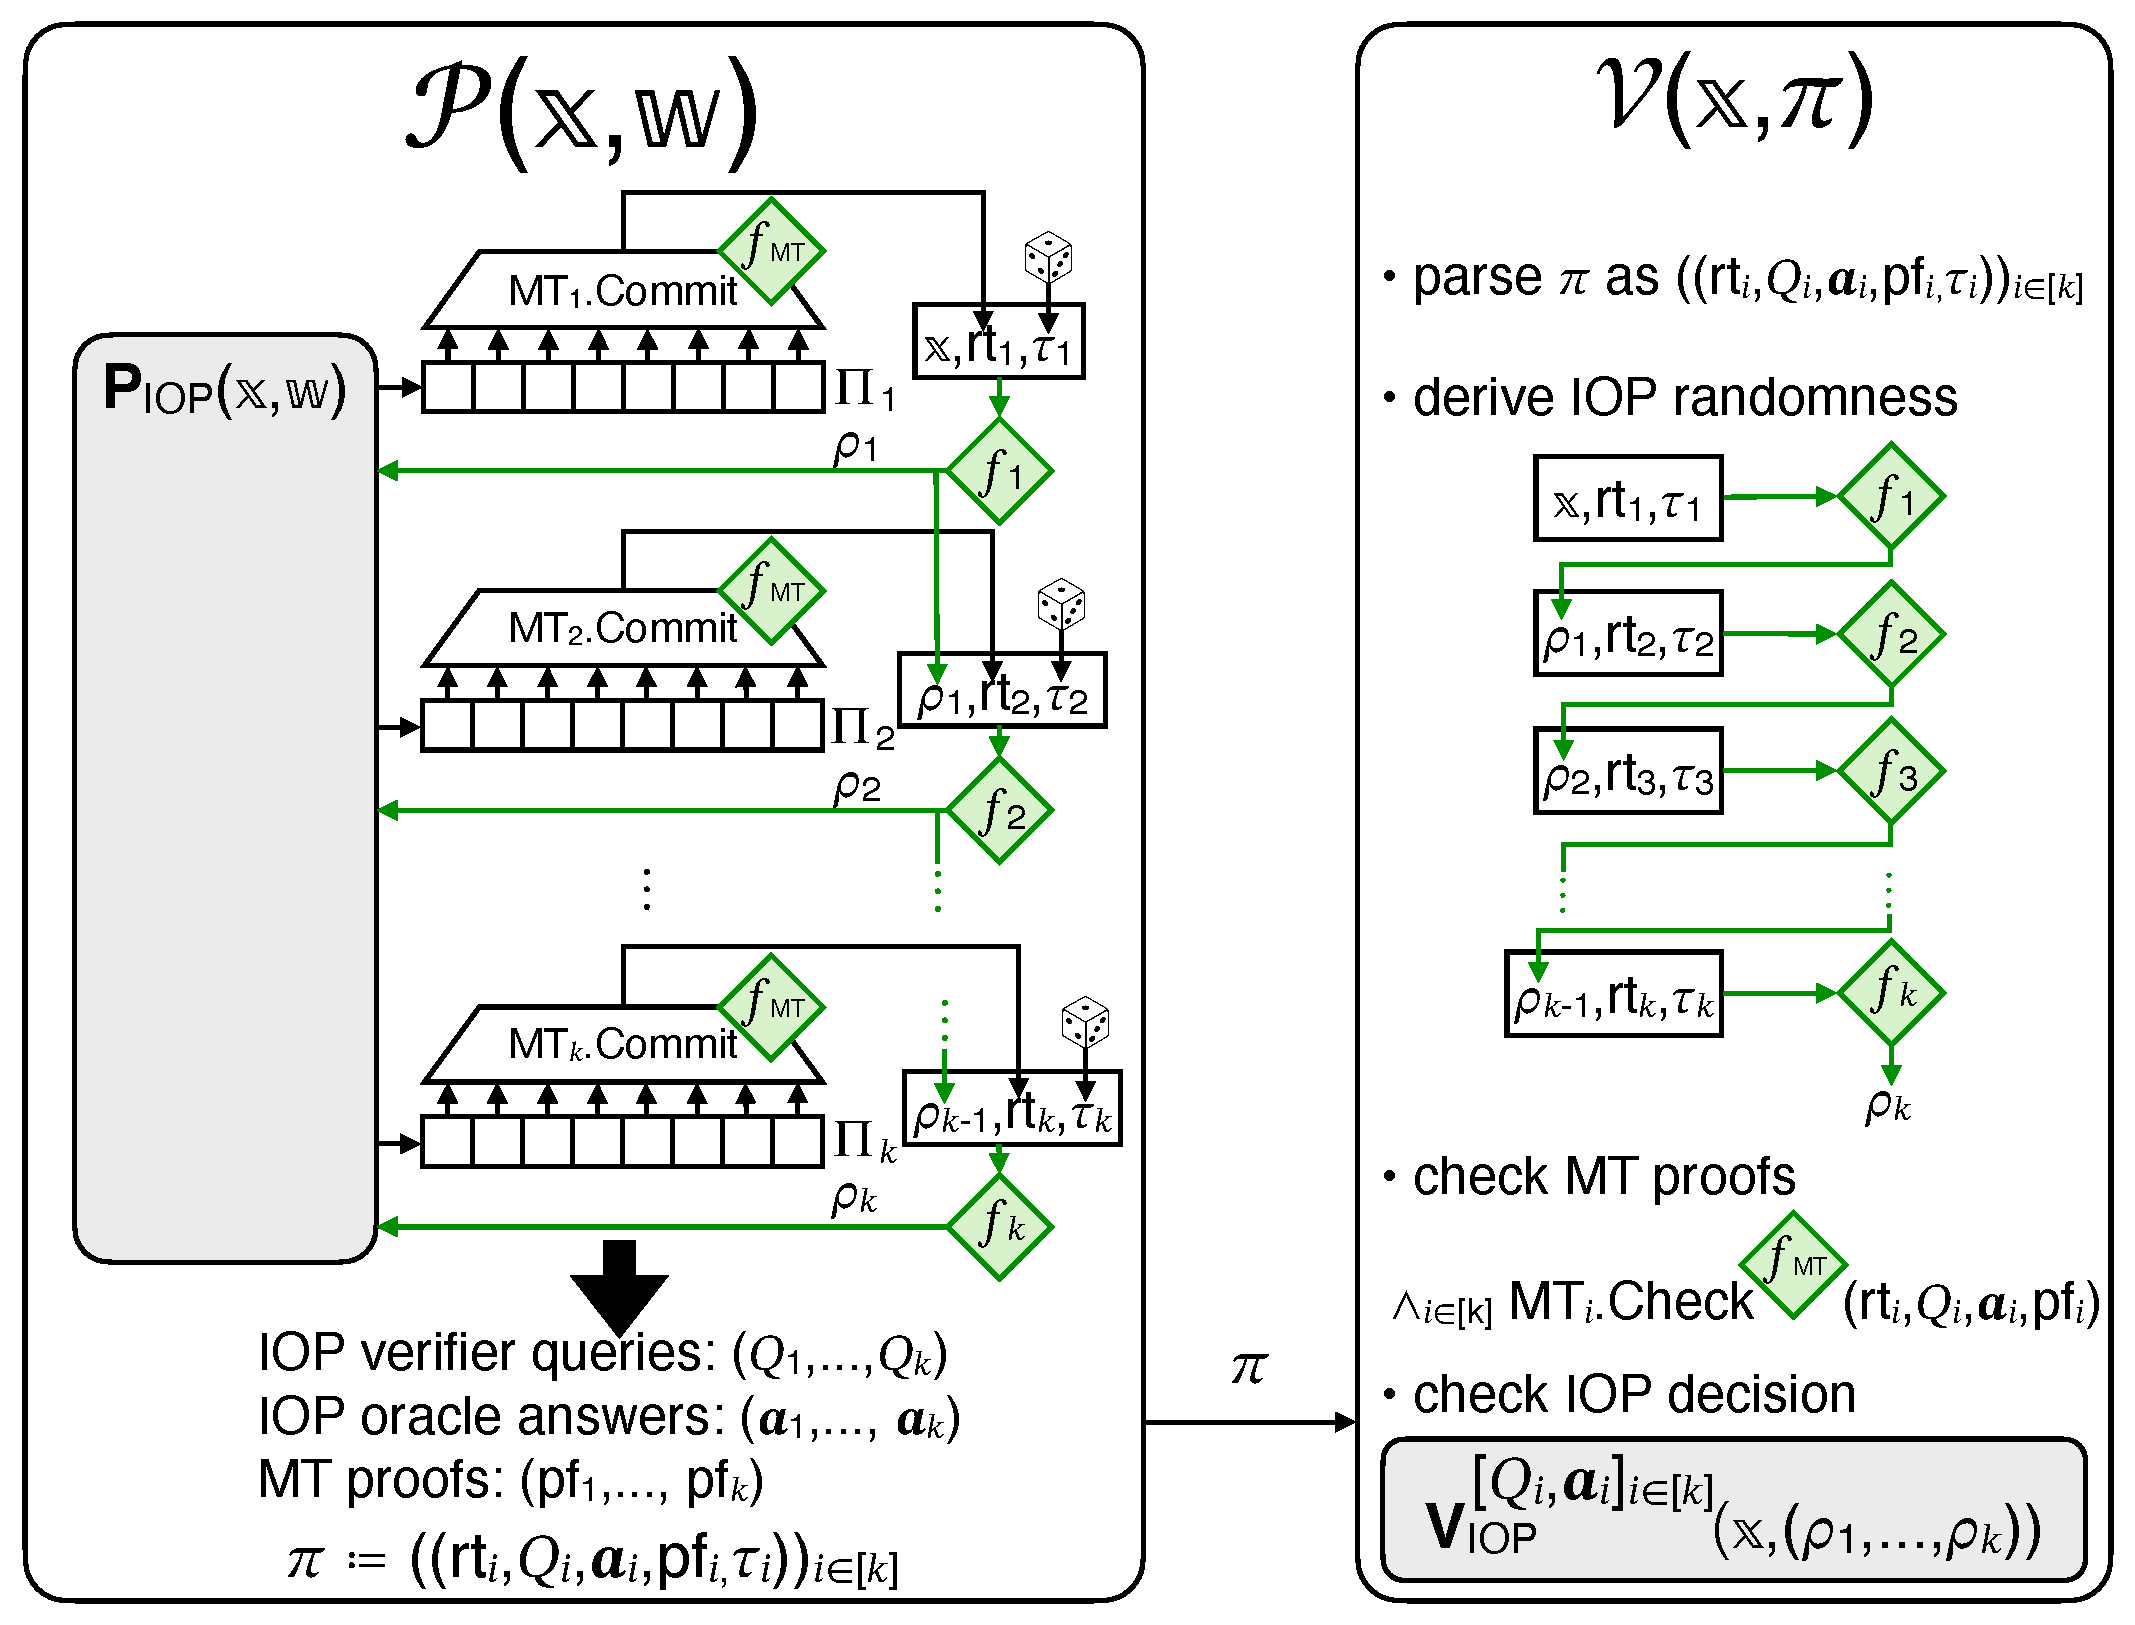
\includegraphics[width=0.8\textwidth]{\FigureFolder/bcs-diagram}
\caption[Diagram of the BCS transformation]{Diagram of the \BCSText ($\BCSSymbol$ in \Cref{construction:bcs-transformation}).}
\label{figure:bcs-diagram}
\end{figure}

%%%%%%%%%%%%%%%%%%%%%%%%%%%%%%%%%%%%%%%%%%%%%%%%%%%%%%%%%%%%%%%%%%%%%%%%%%%%%%%
%%%%%%%%%%%%%%%%%%%%%%%%%%%%%%%%%%%%%%%%%%%%%%%%%%%%%%%%%%%%%%%%%%%%%%%%%%%%%%%
%%%%%%%%%%%%%%%%%%%%%%%%%%%%%%%%%%%%%%%%%%%%%%%%%%%%%%%%%%%%%%%%%%%%%%%%%%%%%%%
\section{Soundness}
\label{section:bcs-soundness}

We prove that \Cref{construction:bcs-transformation} is adaptively sound. The following theorem states that the adaptive soundness error of the non-interactive argument is upper bounded by the IOP state-restoration soundness error of the underlying IOP plus a small error term. The error term has two parts: one part represents the probability of \DoQuote{breaking} the Merkle commitment scheme used to commit to IOP strings; and the other part represents the probability of \DoQuote{breaking} the hash-chain of IOP randomness strings. The fact that the upper bound depends on the IOP state-restoration soundness error, rather than the IOP (standard) soundness error, is expected, due to the use of the Fiat--Shamir transformation.

\begin{ImportantTheorem}{}{bcs-soundness}
Let $\IOPSymbol$ be a public-coin IOP for a relation $\Relation$ with state-restoration soundness error $\IOPSRSoundnessError$ (see \Cref{definition:iop-state-restoration-soundness}), round complexity $\IOPRoundComplexity$, and proof length $\IOPProofLength$. For every security parameter $\SecurityParameter \in \Naturals$ and privacy parameter $\PrivacyParameter \in \Naturals$, $\NARGSymbol \DefineEqual \BCSTransformation{\IOPSymbol}{\SecurityParameter}{\PrivacyParameter}$ in \Cref{construction:bcs-transformation} is a non-interactive argument for $\Relation$ with adaptive soundness error $\ARGSoundnessError$ (see \Cref{definition:narg-adaptive-soundness-with-cnf}) such that
\begin{equation*}
\ARGSoundnessError(\SecurityParameter,\ROQueryBound,\InstanceSize)
\leq
\BCSSoundnessExpression
\enspace.
\end{equation*}
Above $\MTMultiMultiExtractionError$ is the Merkle commitment multi-extraction error from \Cref{lemma:mt-multi-configuration-multi-extractability}. If $\MTMultiMultiExtractabilityCondition{\ROQueryBound}{\IOPRoundComplexity}{\log\IOPProofLength}$, then $\ARGSoundnessError(\SecurityParameter,\ROQueryBound,\InstanceSize) \leq \IOPSRSoundnessError(\SecurityParameter+\RandSaltSize,\ROQueryBound,\InstanceSize) + \BCSSimplifiedError$.
\end{ImportantTheorem}

We discuss two natural approaches to prove the theorem. In \Cref{sec:bcs-direct-soundness-analysis} we outline one approach, and in \Cref{sec:bcs-modular-soundness-analysis} we work out the other approach.

%%%%%%%%%%%%%%%%%%%%%%%%%%%%%%%%%%%%%%%%%%%%%%%%%%%%%%%%%%%%%%%%%%%%%%%%%%%%%%%
%%%%%%%%%%%%%%%%%%%%%%%%%%%%%%%%%%%%%%%%%%%%%%%%%%%%%%%%%%%%%%%%%%%%%%%%%%%%%%%
\subsection{Direct approach}
\label{sec:bcs-direct-soundness-analysis}

\Cref{theorem:bcs-soundness} can be proved by reducing an argument prover $\Malicious{\ARGProver}$ to a corresponding IOP state-restoration prover $\IOPMaliciousSRProver$, relying on the security properties of Merkle commitment schemes and hash chains (each of which introduces a small error). The lemma below captures this reduction and directly implies the theorem using the fact that $\RORandQueryBound,\ROTreeQueryBound \leq \ROQueryBound$.

\begin{lemma}
\label{lemma:bcs-soundness-reduction}
There exists an IOP state-restoration prover $\IOPMaliciousSRProver$ such that, for every $(\ROTreeQueryBound,\RORandQueryBound)$-query argument prover $\Malicious{\ARGProver}$, $\IOPMaliciousSRProver(\BlackBox{\Malicious{\ARGProver}})$ makes at most $\RORandQueryBound$ moves and the following holds:
\begin{align*}
&\Pr\left[
\begin{array}{l}
\SomeSize{\Instance} \leq \InstanceSize \\
\land\;\Instance \notin \GetLanguage{\Relation} \\
\land\;\ARGVerifier^{\ROFunction}(\Instance,\ARGString)=1
\end{array}
\GivenExperiment
\StateExperiment{
\ROFunction=(\ROTreeFunction,(\RORandRoundFunction{\RoundIndex})_{\RoundIndex \in [\IOPRoundComplexity]}) \gets \RODistribution{(\SecurityParameter,\IOPTuple{\IOPRandomnessComplexity})} \\
(\Instance,\ARGString) \gets \Malicious{\ARGProver}^{\ROFunction}
}
\right] \\
&\leq
\Pr\left[
\begin{array}{l}
\SomeSize{\Instance} \leq \InstanceSize \\
\land\;\Instance \notin \GetLanguage{\Relation} \\
\land\;\IOPConvincingCondition=1
\end{array}
\GivenExperiment
\StateExperiment{
\ROTreeFunction \gets \RODistribution{\SecurityParameter} \\
\SRRandomness=\IOPTuple{\SRRandomness} \gets \RODistribution{\IOPTuple{\IOPRandomnessComplexity}} \\
\LongExecution{\IOPSROutput}{\IOPStateRestorationGame{\SecurityParameter+\RandSaltSize}{\SRRandomness}{(\IOPMaliciousSRProver(\BlackBox{\Malicious{\ARGProver}}))^{\ROTreeFunction})}}
}
\right]
\\ & \quad\quad +
\MTMultiMultiExtractionError(\SecurityParameter,\ROTreeQueryBound,\IOPProofLength,(\RORandQueryBound+1)\cdot\IOPRoundComplexity,\IOPRoundComplexity)
+ \frac{\RORandQueryBound^2}{2^{\SecurityParameter}}
\enspace.
\end{align*}
Moreover, the running time of $\IOPMaliciousSRProver$ is bounded by
\begin{equation*}
\ARGTimeP
+ \MTMultiMultiExtractorTimeFunction{\SecurityParameter}{\IOPAlphabet}{\IOPProofLength}{\PrivacyParameter}{\ROTreeQueryBound}{(\RORandQueryBound+1) \cdot \IOPRoundComplexity}
+ O(\IOPMaxRandomnessComplexity \cdot \IOPRoundComplexity \cdot \RORandQueryBound \cdot \log \RORandQueryBound)
\enspace,
\end{equation*}
where $\ARGTimeP$ is the running time of $\Malicious{\ARGProver}$ and $\MTMultiMultiExtractorTimeSymbol$ is the time complexity of the Merkle commitment multi-extractor in \Cref{lemma:mt-multi-configuration-multi-extractability}.
\end{lemma}

We do not prove the lemma (we work out the other approach in \Cref{sec:bcs-modular-soundness-analysis} instead). Nevertheless in \Cref{construction:bcs-direct-reduction} below we describe how to construct $\IOPMaliciousSRProver$ from $\Malicious{\ARGProver}$, as it aids in understanding the security reduction; also state in \Cref{claim:bcs-reduction} the key clai to proving the above lemma. We recommend comparing the construction of $\IOPMaliciousSRProver$ to the construction of $\PCPMaliciousSRProver$ for the Micali transformation in \Cref{construction:micali-reduction}.

\begin{construction}
\label{construction:bcs-direct-reduction}
Let $\MTMultiExtractor$ be the Merkle commitment multi-extractor for $(\MTSymbol_{\RoundIndex})_{\RoundIndex \in [\IOPRoundComplexity]}$ from \Cref{lemma:mt-multi-configuration-multi-extractability} in \Cref{section:merkle-commitment-multi-extractability}; below we use the notation for $\MTMultiExtractor$ introduced in \Cref{remark:mt-multi-extractor-multiple-roots}. Let $\FSTranscriptExtractor$ be the procedure in \Cref{definition:fast-fs-chain-backtrack} (used in the analysis of the Fiat--Shamir transformation). The IOP state-restoration prover $\IOPMaliciousSRProver \DefineEqual \IOPMaliciousSRProver(\BlackBox{\Malicious{\ARGProver}})$ works as follows.
\begin{enumerate}[noitemsep]
  \item For every $\RoundIndex \in [\IOPRoundComplexity]$, lazily sample an oracle $\LazySub{\ROFunctionAlt}{\RoundIndex} \gets \RODistribution{\IOPRandomnessComplexity_{\RoundIndex}}$ (to be used as auxiliary randomness).
  \item Initialize an empty query-answer trace $\ROTreeTrace$.
  \item Simulate $\Malicious{\ARGProver}$ while answering its queries as described below.
  \item When $\Malicious{\ARGProver}$ performs a query to the oracle $\ROTreeFunction$, answer according to $\ROTreeFunction$ and append the resulting query-answer pair to $\ROTreeTrace$.
  \item When $\Malicious{\ARGProver}$ performs a query $\ROQuery$ to the oracle $\RORandRoundFunction{\RoundIndex}$ (for $\RoundIndex \in [\IOPRoundComplexity]$), do the following:
  \begin{enumerate}[nolistsep]
    \item Let $\ROTrace \subseteq \ROTreeTrace$ be the query-answer pairs for $\ROTreeFunction$ between the previous iteration and the current iteration (or the beginning, if this is the first iteration).
    \item If $\RoundIndex=1$ and $\ROQuery$ looks like a query $\BCSFSFirstQuery$:
    \begin{enumerate}[nolistsep]
    \item Run the Merkle extractor: $(\IOPString_{1},\MTTrapdoor_{1}) \DefineEqual \MTMultiExtractor(1,\MTCommitment_{1},\ROTrace)$.
    \item Set the salt string $\SRSaltString_{1} \DefineEqual (\MTCommitment_{1},\RandSaltString_{1})$.
    \item Output the move $(\Instance,\IOPString_{1},\SRSaltString_{1})$ for the IOP state-restoration game.
    \item Receive IOP randomness $\IOPVerifierRandomMessage_{1} \in \Bits^{\IOPRandomnessComplexity_{1}}$ from the game.
    \end{enumerate}
    \item If $\RoundIndex \in \{2,\dots,\IOPRoundComplexity\}$ and $\ROQuery$ looks like a query $\BCSFSLaterQuery{\RoundIndex}$:
    \begin{enumerate}[nolistsep]
      \item Let $\ROTrace_{\FastFSSymbol}$ be the query-answer trace of $\Malicious{\ARGProver}$ to $(\RORandRoundFunction{\RoundIndex})_{\RoundIndex \in [\IOPRoundComplexity]}$ (so far).
      \item Compute $\big(\Instance,(\MTCommitment_{1},\dots,\MTCommitment_{\RoundIndex-1}),(\RandSaltString_{1},\dots,\RandSaltString_{\RoundIndex-1})\big) \DefineEqual \FSTranscriptExtractor(\RoundIndex-1, \IOPVerifierRandomMessage_{\RoundIndex-1}, \ROTrace_{\FastFSSymbol})$.
      \item If $\FSTranscriptExtractor$ aborted then set $\IOPVerifierRandomMessage_{\RoundIndex} \DefineEqual \LazySub{\ROFunctionAlt}{\RoundIndex}(\ROQuery)$ and skip to \Cref{item:bcs-direct-reduction:answer-query}.
      \item Compute $((\IOPString_{1},\MTTrapdoor_{1}),\dots,(\IOPString_{\RoundIndex},\MTTrapdoor_{\RoundIndex})) \DefineEqual \MTMultiExtractor((1,\dots,\RoundIndex),(\MTCommitment_{1},\dots,\MTCommitment_{\RoundIndex}),\ROTrace)$.
      \item For every $j \in [\RoundIndex]$, set the salt string $\SRSaltString_{j} \DefineEqual (\MTCommitment_{j},\RandSaltString_{j})$.
      \item Output the move $\IOPSRGameStateEntry{\RoundIndex}$ for the IOP state-restoration game.
      \item Receive IOP randomness $\IOPVerifierRandomMessage_{\RoundIndex} \in \Bits^{\IOPRandomnessComplexity_{\RoundIndex}}$ from the game.
    \end{enumerate}
    \item Otherwise set $\IOPVerifierRandomMessage_{\RoundIndex} \DefineEqual \LazySub{\ROFunctionAlt}{\RoundIndex}(\ROQuery)$.
    \item \label{item:bcs-direct-reduction:answer-query}
    Return $\IOPVerifierRandomMessage_{\RoundIndex}$ to $\Malicious{\ARGProver}$ as the answer to its query.
  \end{enumerate}
  \item Let $(\Instance,\ARGString)$ be the output of $\Malicious{\ARGProver}$ when it halts, and parse $\ARGString$ as $\BCSARGString$.
  \item Let $\ROTrace' \subseteq \ROTreeTrace$ be the query-answer pairs for $\ROTreeFunction$ between the last iteration and $\Malicious{\ARGProver}$'s halting.
  \item Run the Merkle extractor: $\big((\IOPString_{\RoundIndex},\MTTrapdoor_{\RoundIndex})\big)_{\RoundIndex \in [\IOPRoundComplexity]} \DefineEqual \MTMultiExtractor((\RoundIndex)_{\RoundIndex \in [\IOPRoundComplexity]},(\MTCommitment_{\RoundIndex})_{\RoundIndex \in [\IOPRoundComplexity]},\ROTrace')$.
  \item For every $\RoundIndex \in [\IOPRoundComplexity]$, set the salt string $\SRSaltString_{\RoundIndex} \DefineEqual (\MTCommitment_{\RoundIndex},\RandSaltString_{\RoundIndex})$.
  \item Set $\DecisionBit_{\MTSubscript} \DefineEqual \idxland{\RoundIndex \in [\IOPRoundComplexity]} \MTIdxCheck{\RoundIndex}^{\ROTreeFunction}(\MTCommitment_{\RoundIndex},\IOPQuerySet_{\RoundIndex},\IOPEntries_{\RoundIndex},\MTProof_{\RoundIndex})=1$. (This bit is only used in the analysis.)
  \item Output $\IOPSRGameStateEntry{\IOPRoundComplexity}$.
\end{enumerate}
The prover $\IOPMaliciousSRProver$ potentially makes a move for every query of $\Malicious{\ARGProver}$ to the oracles $(\RORandRoundFunction{\RoundIndex})_{\RoundIndex \in [\IOPRoundComplexity]}$ (no other moves are performed). Since $\Malicious{\ARGProver}$ makes at most $\RORandQueryBound$ queries to $(\RORandRoundFunction{\RoundIndex})_{\RoundIndex \in [\IOPRoundComplexity]}$, $\IOPMaliciousSRProver$ performs at most $\RORandQueryBound$ moves. Next, we discuss the running time of $\IOPMaliciousSRProver$. The simulation of $\Malicious{\ARGProver}$ takes time $\ARGTimeP$, the running time of $\Malicious{\ARGProver}$. Moreover, $\IOPMaliciousSRProver$, performs at most $\RORandQueryBound$ calls to $\FSTranscriptExtractor$; $\IOPMaliciousSRProver$ can ensure that the query-answer trace $\ROTrace_{\FastFSSymbol}$ given as input to $\FSTranscriptExtractor$ is already sorted (lexicographically by answer and then by query), which takes time $\IOPMaxRandomnessComplexity \cdot \RORandQueryBound \cdot \log \RORandQueryBound$, and then each call to $\FSTranscriptExtractor$ takes time $\IOPRoundComplexity \cdot \IOPMaxRandomnessComplexity \cdot \log \RORandQueryBound$ (see \Cref{definition:fast-fs-chain-backtrack}). Finally, $\IOPMaliciousSRProver$ performs at most $(\RORandQueryBound+1) \cdot \IOPRoundComplexity$ calls and Merkle commitment extractions ($\Malicious{\ARGProver}$ makes at most $\RORandQueryBound$ queries to $(\RORandRoundFunction{\RoundIndex})_{\RoundIndex \in [\IOPRoundComplexity]}$ each leading to up to $\IOPRoundComplexity$ Merkle commitment extractions and a final output leading to $\IOPRoundComplexity$ Merkle commitment extractions). The total time for all extractions is given by the expression $\MTMultiMultiExtractorTimeFunction{\SecurityParameter}{\IOPAlphabet}{\IOPProofLength}{\PrivacyParameter}{\ROTreeQueryBound}{(\RORandQueryBound+1) \cdot \IOPRoundComplexity}$ where $\MTMultiMultiExtractorTimeSymbol$ is the (total) time complexity of $\MTMultiExtractor$ in \Cref{lemma:mt-multi-configuration-multi-extractability}.

Overall, running time of $\IOPMaliciousSRProver$ equals the running time of $\Malicious{\ARGProver}$ plus $\MTMultiMultiExtractorTimeFunction{\SecurityParameter}{\IOPAlphabet}{\IOPProofLength}{\PrivacyParameter}{\ROTreeQueryBound}{(\RORandQueryBound+1) \cdot \IOPRoundComplexity} + O(\IOPMaxRandomnessComplexity \cdot \IOPRoundComplexity \cdot \RORandQueryBound \cdot \log \RORandQueryBound)$.
\end{construction}

\begin{claim}
\label{claim:bcs-reduction}
For every $(\ROTreeQueryBound,\RORandQueryBound)$-query argument prover $\Malicious{\ARGProver}$, $\IOPMaliciousSRProver(\BlackBox{\Malicious{\ARGProver}})$ in \Cref{construction:bcs-direct-reduction} makes at most $\RORandQueryBound$ moves and the statistical distance of the following two distribution is upper bounded by $\MTMultiMultiExtractionError(\SecurityParameter,\ROTreeQueryBound,\IOPProofLength,(\RORandQueryBound+1)\cdot\IOPRoundComplexity,\IOPRoundComplexity) + \frac{\RORandQueryBound^2}{2^{\SecurityParameter}}$:
\begin{align*}
&
\left\{
  (\ROTreeTrace,\IOPVerifierRandomMessages,\Instance,\IOPStrings,\DecisionBit)
\GivenExperiment
\StateExperiment{
  \ROFunction=(\ROTreeFunction,(\RORandRoundFunction{\RoundIndex})_{\RoundIndex \in [\IOPRoundComplexity]}) \gets \RODistribution{(\SecurityParameter,\IOPTuple{\IOPRandomnessComplexity})} \\
  \ROOutputAndTrace{\ROFunction}{\Malicious{\ARGProver}}{\ROTrace}{(\Instance,\ARGString=\BCSARGString)} \\
  \big((\IOPString_{\RoundIndex},\MTTrapdoor_{\RoundIndex})\big)_{\RoundIndex \in [\IOPRoundComplexity]} \DefineEqual \MTMultiExtractor((\RoundIndex)_{\RoundIndex \in [\IOPRoundComplexity]},(\MTCommitment_{\RoundIndex})_{\RoundIndex \in [\IOPRoundComplexity]},\ROTreeTrace) \\
  \DecisionBit \xleftarrow{\ROTraceVerifier} \ARGVerifier^{\ROFunction}(\Instance,\ARGString) \\
  \text{parse} \; \ROTraceVerifier \; \text{as} \;  ((\ROQuery_{\RoundIndex},\IOPVerifierRandomMessage_{\RoundIndex}))_{\RoundIndex \in [\IOPRoundComplexity]}
}
\right\}
\quad \text{and} \quad
\\ &
\left\{
  (\ROTreeTrace,\IOPVerifierRandomMessages,\Instance,\IOPStrings,\DecisionBit)
\GivenExperiment
\StateExperiment{
  \ROTreeFunction \gets \RODistribution{\SecurityParameter} \\
\SRRandomness=\IOPTuple{\SRRandomness} \gets \RODistribution{\IOPTuple{\IOPRandomnessComplexity}} \\
  \LongExecutionBelow{\IOPSROutput}{\IOPStateRestorationGame{\SecurityParameter+\RandSaltSize}{\SRRandomness}{(\IOPMaliciousSRProver(\BlackBox{\Malicious{\ARGProver}}))^{\ROTreeFunction})}}{\ROTreeTrace,\DecisionBit_{\MTSubscript}} \\
  \DecisionBit \DefineEqual \IOPVerifier^{\IOPStrings}\big(\IOPVerifierInput\big) \land \DecisionBit_{\MTSubscript}
}
\right\}
\enspace.
\end{align*}
\end{claim}


%%%%%%%%%%%%%%%%%%%%%%%%%%%%%%%%%%%%%%%%%%%%%%%%%%%%%%%%%%%%%%%%%%%%%%%%%%%%%%%
%%%%%%%%%%%%%%%%%%%%%%%%%%%%%%%%%%%%%%%%%%%%%%%%%%%%%%%%%%%%%%%%%%%%%%%%%%%%%%%
\subsection{Modular approach}
\label{sec:bcs-modular-soundness-analysis}

We prove \Cref{theorem:bcs-soundness} via a modular approach, as we explain. The non-interactive argument $\ARGSystem = \BCSTransformation{\IOPSymbol}{\SecurityParameter}{\PrivacyParameter}$ in \Cref{construction:bcs-transformation} is the result of applying (the faster variant of) the Fiat--Shamir transformation $\FastFSonIPTransformation{\IARGSymbol}{\SecurityParameter}{\PrivacyParameter}$ in \Cref{construction:fast-fs-for-public-coin-ip} to the interactive argument $\IARGSymbol = (\IBCSProver,\IBCSVerifier)=\IBCSTransformation{\IOPSymbol}{\SecurityParameter}{\PrivacyParameter}$ in \Cref{construction:ibcs-transformation}. In other words,
\begin{equation}
\label{equation:bcs-as-fs-applied-to-ibcs}
\BCSTransformation{\IOPSymbol}{\SecurityParameter}{\PrivacyParameter}
= \FastFSonIPTransformation{\IBCSTransformation{\IOPSymbol}{\SecurityParameter}{\PrivacyParameter}}{\SecurityParameter}{\PrivacyParameter}
\enspace.
\end{equation}
Note that the Fiat--Shamir transformation is applied to an interactive \emph{argument} $\IARGSymbol$ in the ROM rather than an interactive \emph{proof} $\IPSymbol$. In particular, we use the fact that the security reduction of the Fiat--Shamir transformation works even if the given interactive protocol has \DoQuote{its own} oracles.

In the interactive argument $\IARGSymbol$, the argument prover $\IBCSProver$ sends $\IOPRoundComplexity+1$ messages, where the first $\IOPRoundComplexity$ messages are Merkle commitments $\IOPTuple{\IOPProverMessage}=\IOPTuple{\MTCommitment}$ and the last message is a tuple $\IOPProverMessage_{\IOPRoundComplexity+1}=\big((\IOPQuerySet_{\RoundIndex},\IOPEntries_{\RoundIndex},\MTProof_{\RoundIndex})\big)_{\RoundIndex \in [\IOPRoundComplexity]}$; the argument verifier $\IBCSVerifier$ sends $\IOPRoundComplexity$ random messages $\IOPVerifierRandomMessages$. In particular, there is no random verifier message in round $\IOPRoundComplexity+1$, which has a minor impact on some notation below.

In light of \Cref{equation:bcs-as-fs-applied-to-ibcs}, we will explain how \Cref{lemma:fast-fs-to-state-restoration} tells us that the adaptive soundness error of the non-interactive argument $\ARGSystem = \BCSTransformation{\IOPSymbol}{\SecurityParameter}{\PrivacyParameter}$ in \Cref{construction:bcs-transformation} is upper bounded by the IP state-restoration soundness error of the interactive argument $\IARGSymbol = (\IBCSProver,\IBCSVerifier)=\IBCSTransformation{\IOPSymbol}{\SecurityParameter}{\PrivacyParameter}$ in \Cref{construction:ibcs-transformation}. We are thus left to upper bound the IP state-restoration soundness error of the interactive argument $\IARGSymbol = (\IBCSProver,\IBCSVerifier)$. We do this in the lemma below, and conclude the proof of the theorem at the end of the section.

\begin{lemma}
\label{lemma:ibcs-sr-soundness-reduction}
There exists an IOP state-restoration prover $\IOPMaliciousSRProver$ such that, for every $\ROTreeQueryBound$-query argument prover $\IBCSMaliciousSRProver$ that makes at most $\RORandQueryBound$ moves in an IP state-restoration game, $\IOPMaliciousSRProver(\BlackBox{\IBCSMaliciousSRProver})$ makes at most $\RORandQueryBound$ moves and the following holds for every instance size bound $\InstanceSize \in \Naturals$:
\begin{align*}
&\Pr
\left[
\begin{array}{l}
  \SomeSize{\Instance} \leq \InstanceSize \\
  \land\;\Instance \notin \GetLanguage{\Relation} \\
  \land\;\IBCSVerifier^{\ROTreeFunction}\IBCSSROutput=1
\end{array}
\GivenExperiment
\StateExperiment{
  \ROTreeFunction \gets \RODistribution{\SecurityParameter} \\
  \SRRandomness=\IOPTuple{\SRRandomness} \gets \RODistribution{\IOPTuple{\IOPRandomnessComplexity}} \\
  \LongExecution{\IBCSSROutput}{\IPStateRestorationGame{\SecurityParameter+\RandSaltSize}{\SRRandomness}{(\IBCSMaliciousSRProver)^{\ROTreeFunction}}}
}
\right]
\\
&\leq
\Pr
\left[
\begin{array}{l}
  \SomeSize{\Instance} \leq \InstanceSize \\
  \land\;\Instance \notin \GetLanguage{\Relation} \\
  \land\;\IOPVerifier^{\IOPStrings}(\IOPVerifierInput)=1
\end{array}
\GivenExperiment
\StateExperiment{
  \ROTreeFunction \gets \RODistribution{\SecurityParameter} \\
  \SRRandomness=\IOPTuple{\SRRandomness} \gets \RODistribution{\IOPTuple{\IOPRandomnessComplexity}} \\
  \LongExecution{\IOPSROutput}{\IOPStateRestorationGame{\SecurityParameter+\RandSaltSize}{\SRRandomness}{(\IOPMaliciousSRProver(\BlackBox{\IBCSMaliciousSRProver}))^{\ROTreeFunction}}}
}
\right]
\\ & \quad\quad +
\MTMultiMultiExtractionError(\SecurityParameter,\ROTreeQueryBound,\IOPProofLength,(\RORandQueryBound+1)\cdot\IOPRoundComplexity,\IOPRoundComplexity)
\enspace.
\end{align*}
Moreover, the running time of $\IOPMaliciousSRProver$ equals the running time of $\IBCSMaliciousSRProver$ plus $\MTMultiMultiExtractorTimeFunction{\SecurityParameter}{\IOPAlphabet}{\IOPProofLength}{\PrivacyParameter}{\ROTreeQueryBound}{(\RORandQueryBound+1)\cdot \IOPRoundComplexity}$ where $\MTMultiMultiExtractorTimeSymbol$ is the time complexity of the Merkle commitment multi-extractor in \Cref{lemma:mt-multi-configuration-multi-extractability}.
\end{lemma}

\begin{construction}
\label{construction:sr-soundness-of-ibcs}
Let $\MTMultiExtractor$ be the Merkle commitment multi-extractor for $(\MTSymbol_{\RoundIndex})_{\RoundIndex \in [\IOPRoundComplexity]}$ from \Cref{lemma:mt-multi-configuration-multi-extractability} in \Cref{section:merkle-commitment-multi-extractability}; below we use the notation for $\MTMultiExtractor$ introduced in \Cref{remark:mt-multi-extractor-multiple-roots}. The IOP state-restoration prover $\IOPMaliciousSRProver \DefineEqual \IOPMaliciousSRProver(\BlackBox{\IBCSMaliciousSRProver})$ works as follows.
\begin{enumerate}[noitemsep]
  \item Initialize an empty query-answer trace $\ROTreeTrace$.
  \item Simulate $\IBCSMaliciousSRProver$ while answering its queries as described below.
  \item When $\IBCSMaliciousSRProver$ performs a query to the oracle $\ROTreeFunction$, answer according to $\ROTreeFunction$ and append the resulting query-answer pair to $\ROTreeTrace$.
  \item When $\IBCSMaliciousSRProver$ performs a move $(\Instance, (\IPProverMessage_{1},\ldots,\IPProverMessage_{\RoundIndex}), (\SRSaltString_{1},\ldots,\SRSaltString_{\RoundIndex}))$ with $\RoundIndex\in[\IOPRoundComplexity]$ and $(\IPProverMessage_{1},\ldots,\IPProverMessage_{\RoundIndex})=(\MTCommitment_{1},\ldots,\MTCommitment_{\RoundIndex})$:
  \begin{enumerate}[noitemsep]
    \item Let $\ROTrace \subseteq \ROTreeTrace$ be the query-answer pairs for $\ROTreeFunction$ between the previous iteration and the current iteration (or the beginning if this is the first iteration).
    \item Compute $((\IOPString_{1},\MTTrapdoor_{1}),\dots,(\IOPString_{\RoundIndex},\MTTrapdoor_{\RoundIndex})) \DefineEqual \MTMultiExtractor((1,\dots,\RoundIndex),(\MTCommitment_{1},\dots,\MTCommitment_{\RoundIndex}),\ROTrace)$.
    \item For every $j \in [\RoundIndex]$, set the salt string $\SRSaltString'_{j} \DefineEqual (\MTCommitment_{j},\SRSaltString_{j})$.
    \item Output the move $(\Instance,(\IOPString_{1},\dots,\IOPString_{\RoundIndex}),(\SRSaltString'_{1},\dots,\SRSaltString'_{\RoundIndex}))$ for the IOP state-restoration game.
    \item Receive IOP randomness $\IOPVerifierRandomMessage_{\RoundIndex} \in \Bits^{\IOPRandomnessComplexity_{\RoundIndex}}$ from the game.
    \item Return $\IOPVerifierRandomMessage_{\RoundIndex}$ to $\IBCSMaliciousSRProver$ as response of the game to its move.
  \end{enumerate}
  \item Finally, $\IBCSMaliciousSRProver$ halts and outputs $(\Instance, (\IPProverMessage_{1},\ldots,\IPProverMessage_{\IOPRoundComplexity},\IPProverMessage_{\IOPRoundComplexity+1}), (\SRSaltString_{1},\ldots,\SRSaltString_{\IOPRoundComplexity}))$, with $(\IPProverMessage_{1},\ldots,\IPProverMessage_{\RoundIndex})=(\MTCommitment_{1},\ldots,\MTCommitment_{\RoundIndex})$ and $\IPProverMessage_{\IOPRoundComplexity+1}=\big((\IOPQuerySet_{\RoundIndex},\IOPEntries_{\RoundIndex},\MTProof_{\RoundIndex})\big)_{\RoundIndex \in [\IOPRoundComplexity]}$.
  \item Let $\ROTrace' \subseteq \ROTreeTrace$ be the query-answer pairs for $\ROTreeFunction$ between the last iteration and $\IBCSMaliciousSRProver$'s halting.
  \item Run the Merkle extractor: $\big((\IOPString_{\RoundIndex},\MTTrapdoor_{\RoundIndex})\big)_{\RoundIndex \in [\IOPRoundComplexity]} \DefineEqual \MTMultiExtractor((\RoundIndex)_{\RoundIndex \in [\IOPRoundComplexity]},(\MTCommitment_{\RoundIndex})_{\RoundIndex \in [\IOPRoundComplexity]},\ROTrace')$.
  \item For every $\RoundIndex \in [\IOPRoundComplexity]$, set the salt string $\SRSaltString'_{\RoundIndex} \DefineEqual (\MTCommitment_{\RoundIndex},\SRSaltString_{\RoundIndex})$.
  \item \label{item:iop-modular-bmt}
  Set $\DecisionBit_{\MTSubscript} \DefineEqual \idxland{\RoundIndex \in [\IOPRoundComplexity]} \MTIdxCheck{\RoundIndex}^{\ROTreeFunction}(\MTCommitment_{\RoundIndex},\IOPQuerySet_{\RoundIndex},\IOPEntries_{\RoundIndex},\MTProof_{\RoundIndex})$. (This decision bit is used in the analysis only.)
  \item Output $\left(\Instance,\IOPStrings,(\SRSaltString'_{\RoundIndex})_{\RoundIndex \in [\IOPRoundComplexity]}\right)$.
\end{enumerate}
The prover $\IOPMaliciousSRProver$ makes a move for every move of $\IBCSMaliciousSRProver$. Since $\IBCSMaliciousSRProver$ makes at most $\RORandQueryBound$ moves, $\IOPMaliciousSRProver$ makes at most $\RORandQueryBound$ moves. In terms of running time, $\IOPMaliciousSRProver$ simulates $\IBCSMaliciousSRProver$ (which takes the running time of $\IBCSMaliciousSRProver$) and additionally performs at most $(\RORandQueryBound+1) \cdot \IOPRoundComplexity$ Merkle commitment extractions ($\IBCSMaliciousSRProver$ makes at most $\RORandQueryBound$ moves each containing up to $\IOPRoundComplexity$ Merkle commitments and a final output containing $\IOPRoundComplexity$ Merkle commitments). The total time for all extractions is given by the expression $\MTMultiMultiExtractorTimeFunction{\SecurityParameter}{\IOPAlphabet}{\IOPProofLength}{\PrivacyParameter}{\ROTreeQueryBound}{(\RORandQueryBound+1)\cdot \IOPRoundComplexity}$ where $\MTMultiMultiExtractorTimeSymbol$ is the (total) time complexity of $\MTMultiExtractor$ in \Cref{lemma:mt-multi-configuration-multi-extractability}.
\end{construction}

\begin{construction}
\label{construction:ip-trace-to-iop-trace}
The function $\IPTraceToIOPTrace$ receives as input a move-response trace $\SRTrace$ and a query-answer trace $\ROTreeTrace$, and outputs a move-response trace $\SRTrace_{\IOPSubscript}$, and works as follows.
\begin{itemize}[noitemsep]
\item[] $\IPTraceToIOPTrace(\SRTrace,\ROTreeTrace)$:
\begin{enumerate}[nolistsep]
  \item Initialize an empty move-response trace $\SRTrace_{\IOPSubscript}$.
  \item For every move $\ROQuery$ in $\SRTrace$:
  \begin{enumerate}[nolistsep]
    \item Let $\IOPVerifierRandomMessage_{\RoundIndex} \in \Bits^{\IOPRandomnessComplexity_{\RoundIndex}}$ be the response to the move $\ROQuery$.
    \item If $\ROQuery=(\Instance, (\IPProverMessage_{1},\ldots,\IPProverMessage_{\RoundIndex}), (\SRSaltString_{1},\ldots,\SRSaltString_{\RoundIndex}))$ with $\RoundIndex\in[\IOPRoundComplexity]$ and $(\IPProverMessage_{1},\ldots,\IPProverMessage_{\RoundIndex})=(\MTCommitment_{1},\ldots,\MTCommitment_{\RoundIndex})$:
    \begin{enumerate}[noitemsep]
      \item Let $\ROTrace \subseteq \ROTreeTrace$ be the query-answer pairs for $\ROTreeFunction$ between the previous iteration and the current iteration (or the beginning if this is the first iteration).
      \item Compute $((\IOPString_{1},\MTTrapdoor_{1}),\dots,(\IOPString_{\RoundIndex},\MTTrapdoor_{\RoundIndex})) \DefineEqual \MTMultiExtractor((1,\dots,\RoundIndex),(\MTCommitment_{1},\dots,\MTCommitment_{\RoundIndex}),\ROTrace)$.
      \item For every $j \in [\RoundIndex]$, set the salt string $\SRSaltString'_{j} \DefineEqual (\MTCommitment_{j},\SRSaltString_{j})$.
      \item Add the move-response pair $\big(\IOPSRGameStateEntry{\RoundIndex},\IOPVerifierRandomMessage_{\RoundIndex}\big)$ to $\SRTrace_{\IOPSubscript}$.
    \end{enumerate}
  \end{enumerate}
  \item Output $\SRTrace_{\IOPSubscript}$.
\end{enumerate}
\end{itemize}
Assume that $\SRTrace$ has size at most $\RORandQueryBound$. The function $\IPTraceToIOPTrace$ can be computed as follows. First, partition the query-answer trace $\ROTreeTrace$ according to the move-response trace $\SRTrace$. This can be done by performing a linear pass on $\ROTreeTrace$ and $\SRTrace$, in time $O(\Cardinality{\ROTreeTrace} + \Cardinality{\SRTrace}) = O(\ROTreeQueryBound + \RORandQueryBound)$. Then, the number of extractions is at most $\RORandQueryBound \cdot \IOPRoundComplexity$ and the total time for all extractions is given by the expression $\MTMultiMultiExtractorTimeFunction{\SecurityParameter}{\IOPAlphabet}{\IOPProofLength}{\PrivacyParameter}{\ROTreeQueryBound}{\RORandQueryBound \cdot \IOPRoundComplexity}$ where $\MTMultiMultiExtractorTimeSymbol$ is the (total) time complexity of $\MTMultiExtractor$ in \Cref{lemma:mt-multi-configuration-multi-extractability}. Therefore, the total running time is at most
\begin{equation*}
O(\ROTreeQueryBound + \RORandQueryBound) + \MTMultiMultiExtractorTimeFunction{\SecurityParameter}{\IOPAlphabet}{\IOPProofLength}{\PrivacyParameter}{\ROTreeQueryBound}{\RORandQueryBound \cdot \IOPRoundComplexity}
\enspace.
\end{equation*}
\end{construction}

\begin{proof}[Proof of \Cref{lemma:ibcs-sr-soundness-reduction}]
We argue that the IOP prover $\IOPMaliciousProver$ in \Cref{construction:sr-soundness-of-ibcs} satisfies the probability statement in the lemma. It suffices to prove the following upper bound:
\begin{align}
\label{eq:iop-modular-soundness-distributions}
\StatisticalDistanceSymbol&\left(\left\{
  (\Instance,\DecisionBit,\SRTrace_{\IOPSubscript},\ROTreeTrace,\IPTuple{\IPVerifierRandomMessage})
\GivenExperiment
\StateExperiment{
  \ROTreeFunction \gets \RODistribution{\SecurityParameter} \\
  \SRRandomness \gets \RODistribution{\IOPTuple{\IOPRandomnessComplexity}} \\
  \LongExecutionOver{\IBCSSROutput}{\IPStateRestorationGame{\SecurityParameter+\RandSaltSize}{\SRRandomness}{(\IBCSMaliciousSRProver)^{\ROTreeFunction}}}{\SRTrace,\ROTreeTrace} \\
  \DecisionBit \gets \IBCSVerifier^{\ROTreeFunction}\IBCSSROutput \\
  \SRTrace_{\IOPSubscript} \DefineEqual \IPTraceToIOPTrace(\SRTrace,\ROTreeTrace)
}
\right\},\right.
\\ \nonumber
&\phantom{aa}\left.\left\{
  (\Instance,\DecisionBit \land \DecisionBit_{\MTSubscript},\SRTrace_{\IOPSubscript},\ROTreeTrace,\IPTuple{\IPVerifierRandomMessage})
\GivenExperiment
\StateExperiment{
  \ROTreeFunction \gets \RODistribution{\SecurityParameter} \\
  \SRRandomness \gets \RODistribution{\IOPTuple{\IOPRandomnessComplexity}} \\
  \LongExecutionOver{\IOPSROutput}{\IOPStateRestorationGame{\SecurityParameter+\RandSaltSize}{\SRRandomness}{(\IOPMaliciousSRProver(\BlackBox{\IBCSMaliciousSRProver}))^{\ROTreeFunction}}}{\SRTrace_{\IOPSubscript},\ROTreeTrace,\DecisionBit_{\MTSubscript}} \\
  \DecisionBit \gets \IOPVerifier^{\IOPStrings}(\IOPVerifierInput)
}
\right\}\right) \\ \nonumber
&\leq \MTMultiMultiExtractionError(\SecurityParameter,\ROTreeQueryBound,\IOPProofLength,(\RORandQueryBound+1)\cdot\IOPRoundComplexity,\IOPRoundComplexity)
\enspace.
\end{align}
Above, on the right-side, $\SRTrace_{\IOPSubscript}$ is the move-response trace of the IOP state-restoration game, $\ROTreeTrace$ is the query-answer trace to the oracle $\ROTreeFunction$, and $\DecisionBit_{\MTSubscript}$ is the internal variable defined in \Cref{item:iop-modular-bmt}.

We begin by considering the left-side distribution. Recall that $\IOPTuple{\IOPProverMessage}=\IOPTuple{\MTCommitment}$ and that $\IOPProverMessage_{\IOPRoundComplexity+1}=\big((\IOPQuerySet_{\RoundIndex},\IOPEntries_{\RoundIndex},\MTProof_{\RoundIndex})\big)_{\RoundIndex \in [\IOPRoundComplexity]}$. Moreover, $\IBCSVerifier$ accepts if and only if the IOP verifier $\IOPVerifier$ accepts and every invocation of the Merkle commitment checking algorithm $\MTCheck$ accepts. Therefore, the left-side distribution equals to:
\begin{align*}
\left\{
(\Instance, \DecisionBit \land \DecisionBit_{\MTSubscript},\SRTrace_{\IOPSubscript},\ROTreeTrace, \IPTuple{\IPVerifierRandomMessage})
\GivenExperiment
\StateExperiment{
  \ROTreeFunction \gets \RODistribution{\SecurityParameter} \\
  \SRRandomness \gets \RODistribution{\IOPTuple{\IOPRandomnessComplexity}} \\
  \LongExecutionOver{\IBCSSROutput}{\IPStateRestorationGame{\SecurityParameter+\RandSaltSize}{\SRRandomness}{(\IBCSMaliciousSRProver)^{\ROTreeFunction}}}{\SRTrace,\ROTreeTrace} \\
  \text{parse } \IOPTuple{\IOPProverMessage} \text{ as } \IOPTuple{\MTCommitment} \\
  \text{parse } \IOPProverMessage_{\IOPRoundComplexity+1} \text{ as } \big((\IOPQuerySet_{\RoundIndex},\IOPEntries_{\RoundIndex},\MTProof_{\RoundIndex})\big)_{\RoundIndex \in [\IOPRoundComplexity]} \\
  \DecisionBit \gets \IOPVerifier^{\IOPLocalView{\IOPQuerySet}{\IOPEntries}}(\IOPVerifierInput) \\
  \DecisionBit_{\MTSubscript} \gets \idxland{\RoundIndex \in [\IOPRoundComplexity]} \MTCheck^{\ROTreeFunction}(\MTCommitment_{\RoundIndex},\IOPQuerySet_{\RoundIndex},\IOPEntries_{\RoundIndex},\MTProof_{\RoundIndex}) \\
  \SRTrace_{\IOPSubscript} \DefineEqual \IPTraceToIOPTrace(\SRTrace,\ROTreeTrace)
}
\right\}
\enspace.
\end{align*}
Define the event $\Event$ as follows:
\begin{align*}
\left[
\begin{array}{l}
  \DecisionBit_{\MTSubscript} = 0 \\
  \lor \;\idxland{\RoundIndex \in [\IOPRoundComplexity]} \IOPString_{\RoundIndex}[\IOPQuerySet_{\RoundIndex}] = \IOPEntries_{\RoundIndex}
\end{array}
\GivenExperiment
\StateExperiment{
  \ROTreeFunction \gets \RODistribution{\SecurityParameter} \\
  \SRRandomness \gets \RODistribution{\IOPTuple{\IOPRandomnessComplexity}} \\
  \LongExecutionOver{\IBCSSROutput}{\IPStateRestorationGame{\SecurityParameter+\RandSaltSize}{\SRRandomness}{(\IBCSMaliciousSRProver)^{\ROTreeFunction}}}{\ROTreeTrace} \\
  \text{parse } \IOPTuple{\IOPProverMessage} \text{ as } \IOPTuple{\MTCommitment} \\
  \text{parse } \IOPProverMessage_{\IOPRoundComplexity+1} \text{ as } \big((\IOPQuerySet_{\RoundIndex},\IOPEntries_{\RoundIndex},\MTProof_{\RoundIndex})\big)_{\RoundIndex \in [\IOPRoundComplexity]} \\
  \DecisionBit \gets \IOPVerifier^{\IOPLocalView{\IOPQuerySet}{\IOPEntries}}(\IOPVerifierInput) \\
  \DecisionBit_{\MTSubscript} \gets \idxland{\RoundIndex \in [\IOPRoundComplexity]} \MTIdxCheck{\RoundIndex}^{\ROTreeFunction}(\MTCommitment_{\RoundIndex},\IOPQuerySet_{\RoundIndex},\IOPEntries_{\RoundIndex},\MTProof_{\RoundIndex}) \\
  ((\IOPString_{\RoundIndex},\MTTrapdoor_{\RoundIndex}))_{\RoundIndex \in [\IOPRoundComplexity]} \DefineEqual \MTMultiExtractor((\RoundIndex)_{\RoundIndex \in [\IOPRoundComplexity]},(\MTCommitment_{\RoundIndex})_{\RoundIndex \in [\IOPRoundComplexity]},\ROTreeTrace) \\
}
\right]
\enspace.
\end{align*}
By \Cref{claim:statistical-distance-condition-event}, it suffices to upper bound the probability of $\Negate{\Event}$ and to show that the two distributions in \Cref{eq:iop-modular-soundness-distributions} are identical when conditioned on $\Event$.

Conditioned on the event $\Event$: either $\DecisionBit_{\MTSubscript}=0$, in which case $\DecisionBit \land \DecisionBit_{\MTSubscript} = 0$ in both sides; or $\DecisionBit_{\MTSubscript}=1$ and $\idxland{\RoundIndex \in [\IOPRoundComplexity]} \IOPString_{\RoundIndex}[\IOPQuerySet_{\RoundIndex}] = \IOPEntries_{\RoundIndex}$ (every extracted IOP string agrees with the relevant query answers), in which case $\IOPVerifier^{\IOPLocalView{\IOPQuerySet}{\IOPEntries}}(\IOPVerifierInput) = \IOPVerifier^{\IOPStrings}(\IOPVerifierInput)$ (the IOP verifier returns the same output), so $\DecisionBit$ is the same on both sides. Therefore, the following two distributions are equivalent:
\begin{align*}
& \left\{
\begin{array}{l}
(\Instance, \DecisionBit \land \DecisionBit_{\MTSubscript},\SRTrace_{\IOPSubscript},\ROTreeTrace, \IPTuple{\IPVerifierRandomMessage}) \\
\ConditionedOnText \\
 \Event
\end{array}
\GivenExperiment
\StateExperiment{
  \ROTreeFunction \gets \RODistribution{\SecurityParameter} \\
  \SRRandomness \gets \RODistribution{\IOPTuple{\IOPRandomnessComplexity}} \\
  \LongExecutionOver{\IBCSSROutput}{\IPStateRestorationGame{\SecurityParameter+\RandSaltSize}{\SRRandomness}{(\IBCSMaliciousSRProver)^{\ROTreeFunction}}}{\SRTrace,\ROTreeTrace} \\
  \text{parse } \IOPTuple{\IOPProverMessage} \text{ as } \IOPTuple{\MTCommitment} \\
  \text{parse } \IOPProverMessage_{\IOPRoundComplexity+1} \text{ as } \big((\IOPQuerySet_{\RoundIndex},\IOPEntries_{\RoundIndex},\MTProof_{\RoundIndex})\big)_{\RoundIndex \in [\IOPRoundComplexity]} \\
  \DecisionBit \gets \IOPVerifier^{\IOPLocalView{\IOPQuerySet}{\IOPEntries}}(\IOPVerifierInput) \\
  \DecisionBit_{\MTSubscript} \gets \idxland{\RoundIndex \in [\IOPRoundComplexity]} \MTCheck^{\ROTreeFunction}(\MTCommitment_{\RoundIndex},\IOPQuerySet_{\RoundIndex},\IOPEntries_{\RoundIndex},\MTProof_{\RoundIndex}) \\
  \SRTrace_{\IOPSubscript} \DefineEqual \IPTraceToIOPTrace(\SRTrace,\ROTreeTrace)
}
\right\}
\\ & \TextAndInMath
\\ &
\left\{
\begin{array}{l}
  (\Instance, \DecisionBit \land \DecisionBit_{\MTSubscript},\SRTrace_{\IOPSubscript},\ROTreeTrace, \IPTuple{\IPVerifierRandomMessage}) \\
 \ConditionedOnText \\
 \Event
\end{array}
\GivenExperiment
\StateExperiment{
  \ROTreeFunction \gets \RODistribution{\SecurityParameter} \\
  \SRRandomness \gets \RODistribution{\IOPTuple{\IOPRandomnessComplexity}} \\
  \LongExecutionOver{\IBCSSROutput}{\IPStateRestorationGame{\SecurityParameter+\RandSaltSize}{\SRRandomness}{(\IBCSMaliciousSRProver)^{\ROTreeFunction}}}{\SRTrace,\ROTreeTrace} \\
  \text{parse } \IOPTuple{\IOPProverMessage} \text{ as } \IOPTuple{\MTCommitment} \\
  \text{parse } \IOPProverMessage_{\IOPRoundComplexity+1} \text{ as } \big((\IOPQuerySet_{\RoundIndex},\IOPEntries_{\RoundIndex},\MTProof_{\RoundIndex})\big)_{\RoundIndex \in [\IOPRoundComplexity]} \\
  ((\IOPString_{\RoundIndex},\MTTrapdoor_{\RoundIndex}))_{\RoundIndex \in [\IOPRoundComplexity]} \DefineEqual \MTMultiExtractor((\RoundIndex)_{\RoundIndex \in [\IOPRoundComplexity]},(\MTCommitment_{\RoundIndex})_{\RoundIndex \in [\IOPRoundComplexity]},\ROTreeTrace) \\
  \DecisionBit \gets \IOPVerifier^{\IOPStrings}(\IOPVerifierInput) \\
  \DecisionBit_{\MTSubscript} \gets \idxland{\RoundIndex \in [\IOPRoundComplexity]} \MTIdxCheck{\RoundIndex}^{\ROTreeFunction}(\MTCommitment_{\RoundIndex},\IOPQuerySet_{\RoundIndex},\IOPEntries_{\RoundIndex},\MTProof_{\RoundIndex}) \\
  \SRTrace_{\IOPSubscript} \DefineEqual \IPTraceToIOPTrace(\SRTrace,\ROTreeTrace)
}
\right\}
\enspace.
\end{align*}
The tuple $\big(\Instance,\IOPStrings,\IOPVerifierRandomMessages\big)$ has the same distribution as the tuple in the output of the IOP state-restoration game $\IOPSROutput$ with the IOP state-restoration prover $\IOPMaliciousSRProver(\BlackBox{\IBCSMaliciousSRProver})$, as can be seen by inspection of \Cref{construction:sr-soundness-of-ibcs}. Moreover, by the construction, the trace of the IOP state-restoration game of $\IOPMaliciousSRProver(\BlackBox{\IBCSMaliciousSRProver})$ is the same as the trace $\SRTrace_{\IOPSubscript} \DefineEqual \IPTraceToIOPTrace(\SRTrace,\ROTreeTrace)$, as can be seen by inspection of \Cref{construction:ip-trace-to-iop-trace}. Hence, the right-side distribution equals:
\begin{equation*}
\left\{
\begin{array}{l}
  (\Instance, \DecisionBit \land \DecisionBit_{\MTSubscript},\SRTrace_{\IOPSubscript},\ROTreeTrace, \IPTuple{\IPVerifierRandomMessage}) \\
 \ConditionedOnText \\
 \Event
\end{array}
\GivenExperiment
\StateExperiment{
  \ROTreeFunction \gets \RODistribution{\SecurityParameter} \\
  \SRRandomness \gets \RODistribution{\IOPTuple{\IOPRandomnessComplexity}} \\
  \LongExecutionOver{\IOPSROutput}{\IOPStateRestorationGame{\SecurityParameter+\RandSaltSize}{\SRRandomness}{(\IOPMaliciousSRProver(\BlackBox{\IBCSMaliciousSRProver}))^{\ROTreeFunction}}}{\SRTrace_{\IOPSubscript},\ROTreeTrace} \\
  \text{parse } \IOPTuple{\IOPProverMessage} \text{ as } \IOPTuple{\MTCommitment} \\
  \text{parse } \IOPProverMessage_{\IOPRoundComplexity+1} \text{ as } \big((\IOPQuerySet_{\RoundIndex},\IOPEntries_{\RoundIndex},\MTProof_{\RoundIndex})\big)_{\RoundIndex \in [\IOPRoundComplexity]} \\
  \DecisionBit \gets \IOPVerifier^{\IOPStrings}(\IOPVerifierInput) \\
  \DecisionBit_{\MTSubscript} \gets \idxland{\RoundIndex \in [\IOPRoundComplexity]} \MTIdxCheck{\RoundIndex}^{\ROTreeFunction}(\MTCommitment_{\RoundIndex},\IOPQuerySet_{\RoundIndex},\IOPEntries_{\RoundIndex},\MTProof_{\RoundIndex})
}
\right\}
\enspace.
\end{equation*}
The above is exactly the right-side distribution of \Cref{eq:iop-modular-soundness-distributions}, conditioned on $\Event$. Thus, by \Cref{claim:statistical-distance-condition-event}, we are left with bounding the probability of the event $\Negate{\Event}$.

The probability of $\Negate{\Event}$ is upper bounded by the Merkle commitment multi-extraction error (\Cref{lemma:mt-multi-configuration-multi-extractability}), and is upper bounded by the following expression:
\begin{equation*}
\Pr
\left[
\begin{array}{l}
  \DecisionBit_{\MTSubscript}=1 \\
  \land\;\idxlor{\RoundIndex \in [\IOPRoundComplexity]} \IOPString_{\RoundIndex}[\IOPQuerySet_{\RoundIndex}] \neq \IOPEntries_{\RoundIndex}
\end{array}
\GivenExperiment
\StateExperiment{
  \ROTreeFunction \gets \RODistribution{\SecurityParameter} \\
  \SRRandomness \gets \RODistribution{\IOPTuple{\IOPRandomnessComplexity}} \\
  \LongExecutionOver{\IOPSROutput}{\IPStateRestorationGame{\SecurityParameter+\RandSaltSize}{\SRRandomness}{(\IBCSMaliciousSRProver)^{\ROTreeFunction}}}{\ROTreeTrace} \\
  \text{parse } \IOPTuple{\IOPProverMessage} \text{ as } \IOPTuple{\MTCommitment} \\
  \text{parse } \IOPProverMessage_{\IOPRoundComplexity+1} \text{ as } \big((\IOPQuerySet_{\RoundIndex},\IOPEntries_{\RoundIndex},\MTProof_{\RoundIndex})\big)_{\RoundIndex \in [\IOPRoundComplexity]} \\
  \DecisionBit_{\MTSubscript} \gets \idxland{\RoundIndex \in [\IOPRoundComplexity]} \MTCheck^{\ROTreeFunction}(\MTCommitment_{\RoundIndex},\IOPQuerySet_{\RoundIndex},\IOPEntries_{\RoundIndex},\MTProof_{\RoundIndex}) \\
  ((\IOPString_{\RoundIndex},\MTTrapdoor_{\RoundIndex}))_{\RoundIndex \in [\IOPRoundComplexity]} \DefineEqual \MTMultiExtractor((\RoundIndex)_{\RoundIndex \in [\IOPRoundComplexity]},(\MTCommitment_{\RoundIndex})_{\RoundIndex \in [\IOPRoundComplexity]},\ROTreeTrace) \\
}
\right]
\enspace.
\end{equation*}
In turn, the above probability is at most $\MTMultiMultiExtractionError(\SecurityParameter,\ROTreeQueryBound,\IOPProofLength, (\RORandQueryBound+1) \cdot \IOPRoundComplexity,\IOPRoundComplexity)$ by \Cref{lemma:mt-multi-configuration-multi-extractability}. Here the function $\MTMultiMultiExtractionError$ gets five parameters: $\SecurityParameter$ is the security parameter, $\ROTreeQueryBound$ is the query bound of $\IBCSMaliciousSRProver$, $\IOPProofLength$ is the IOP proof length (a bound on message length), $(\RORandQueryBound+1) \cdot \IOPRoundComplexity$ is the number of output Merkle commitments ($\IBCSMaliciousSRProver$ makes at most $\RORandQueryBound$ moves each containing up to $\IOPRoundComplexity$ Merkle commitments and a final output containing $\IOPRoundComplexity$ Merkle commitments), and $\IOPRoundComplexity$ is the number of opened Merkle commitments ($\IBCSMaliciousSRProver$ produces $\IOPRoundComplexity$ openings).
\end{proof}

\begin{proof}[Proof of \Cref{theorem:bcs-soundness}]
\Cref{lemma:ibcs-sr-soundness-reduction} tells us that the interactive argument $\IARGSymbol = (\IBCSProver,\IBCSVerifier)=\IBCSTransformation{\IOPSymbol}{\SecurityParameter}{\PrivacyParameter}$ in \Cref{construction:ibcs-transformation} has IP state-restoration soundness error
\begin{equation*}
\IPSRSoundnessError(\PrivacyParameter,\RORandQueryBound,\InstanceSize)
\leq
\IOPSRSoundnessError(\SecurityParameter + \PrivacyParameter,\RORandQueryBound,\InstanceSize)
+ \MTMultiMultiExtractionError(\SecurityParameter,\ROTreeQueryBound,\IOPProofLength,(\RORandQueryBound+1)\cdot\IOPRoundComplexity,\IOPRoundComplexity)
\end{equation*}
against adversaries that make at most $\ROTreeQueryBound$ queries to the random oracle $\ROTreeFunction$.

Next, consider the non-interactive argument $\FastFSonIPTransformation{\IARGSymbol}{\SecurityParameter}{\PrivacyParameter}=\BCSTransformation{\IOPSymbol}{\SecurityParameter}{\PrivacyParameter}$ in \Cref{construction:bcs-transformation}. Fix a malicious argument prover $\Malicious{\ARGProver}$ for $\FastFSonIPTransformation{\IARGSymbol}{\SecurityParameter}{\PrivacyParameter}$ that makes $\RORandQueryBound$ queries to oracles $(\RORandRoundFunction{\RoundIndex})_{\RoundIndex \in [\IOPRoundComplexity]}$ and $\ROTreeQueryBound$ queries to oracle $\ROTreeFunction$. We now explain how to apply \Cref{lemma:fast-fs-to-state-restoration} to obtain a reduction from the malicious argument prover $\Malicious{\ARGProver}$ to an IP state-restoration prover $\IBCSMaliciousSRProver(\BlackBox{\Malicious{\ARGProver}})$ for the interactive argument $\IARGSymbol = (\IBCSProver,\IBCSVerifier)=\IBCSTransformation{\IOPSymbol}{\SecurityParameter}{\PrivacyParameter}$ (in which the argument prover and argument verifier have access to the random oracle $\ROTreeFunction$). Recall that the transformation $\FastFSonIPSymbol$ introduces random oracles $(\RORandRoundFunction{\RoundIndex})_{\RoundIndex \in [\IOPRoundComplexity]}$ to transform an IP into a non-interactive argument, and \Cref{lemma:fast-fs-to-state-restoration} captures the security of this transformation by providing a reduction that transforms a malicious argument prover $\Malicious{\ARGProver}$ against the non-interactive argument into an IP state-restoration prover $\IPMaliciousSRProver(\BlackBox{\Malicious{\ARGProver}})$ for the IP state-restoration game of the underling IP. However here we apply the transformation $\FastFSonIPSymbol$ to the interactive argument $\IARGSymbol = (\IBCSProver,\IBCSVerifier)=\IBCSTransformation{\IOPSymbol}{\SecurityParameter}{\PrivacyParameter}$, which uses a random oracle $\ROTreeFunction$. Nevertheless, \Cref{lemma:fast-fs-to-state-restoration} still works in this case because the reduction makes only black-box use of the given non-interactive argument prover $\Malicious{\ARGProver}$, and hence it does not matter if $\Malicious{\ARGProver}$ has access to an additional oracle $\ROTreeFunction$ (separate from the oracles $(\RORandRoundFunction{\RoundIndex})_{\RoundIndex \in [\IOPRoundComplexity]}$ introduced by $\FastFSonIPSymbol$). To make explicit this difference, we use the notation $\IBCSMaliciousSRProver(\BlackBox{\Malicious{\ARGProver}})$ to refer to $\IPMaliciousSRProver(\BlackBox{\Malicious{\ARGProver}})$ where $\IPMaliciousSRProver$ is augmented to forward queries from $\Malicious{\ARGProver}$ to $\ROTreeFunction$ and return the corresponding answers.

Therefore, by \Cref{lemma:fast-fs-to-state-restoration}, we deduce the following:
\begin{align*}
&\Pr\left[
\begin{array}{l}
  \SomeSize{\Instance} \leq \InstanceSize \\
  \land\;\Instance \notin \GetLanguage{\Relation} \\
  \land\;\ARGVerifier^{\ROFunction}(\Instance,\ARGString) = 1
\end{array}
\GivenExperiment
\StateExperiment{
  (\RORandRoundFunction{\RoundIndex})_{\RoundIndex \in [\IOPRoundComplexity]} \gets \RODistribution{\IOPTuple{\IOPRandomnessComplexity}} \\
  \ROTreeFunction \gets \RODistribution{\SecurityParameter} \\
  \ROFunction \DefineEqual (\ROTreeFunction,(\RORandRoundFunction{\RoundIndex})_{\RoundIndex \in [\IOPRoundComplexity]}) \\
  (\Instance,\ARGString) \gets \Malicious{\ARGProver}^{\ROFunction}
}
\right]
\\ \leq &
\Pr
\left[
\begin{array}{l}
  \SomeSize{\Instance} \leq \InstanceSize \\
  \land\;\Instance \notin \GetLanguage{\Relation} \\
  \land\;\IBCSVerifier^{\ROTreeFunction}\IBCSSROutput=1
\end{array}
\GivenExperiment
\StateExperiment{
  \ROTreeFunction \gets \RODistribution{\SecurityParameter} \\
  \SRRandomness=\IOPTuple{\SRRandomness} \gets \RODistribution{\IOPTuple{\IOPRandomnessComplexity}} \\
  \LongExecution{\IBCSSROutput}{\IPStateRestorationGame{\SecurityParameter+\RandSaltSize}{\SRRandomness}{(\IBCSMaliciousSRProver(\BlackBox{\Malicious{\ARGProver}}))^{\ROTreeFunction}}}
}
\right]
\\ & \phantom{aaa} + \FSErrorExpression[\RORandQueryBound]
\enspace.
\end{align*}
This tells us that the non-interactive argument $\FastFSonIPTransformation{\IARGSymbol}{\SecurityParameter}{\PrivacyParameter}=\BCSTransformation{\IOPSymbol}{\SecurityParameter}{\PrivacyParameter}$ in \Cref{construction:bcs-transformation} has adaptive soundness error
\begin{equation*}
\ARGSoundnessError(\SecurityParameter,\RORandQueryBound,\InstanceSize)
\leq
\IPSRSoundnessError(\PrivacyParameter,\RORandQueryBound,\InstanceSize)
+ \FSErrorExpression[\RORandQueryBound]
\end{equation*}
where $\IPSRSoundnessError$ is the IP state-restoration soundness error of $\IARGSymbol$.

Using the fact that $\RORandQueryBound,\ROTreeQueryBound \leq \ROQueryBound$, we conclude that \Cref{construction:bcs-transformation} has adaptive soundness error
\begin{equation*}
\ARGSoundnessError(\SecurityParameter,\ROQueryBound,\InstanceSize)
\leq
\IPSRSoundnessError(\PrivacyParameter,\ROQueryBound,\InstanceSize)
+
\FSErrorExpression
\leq
\IOPSRSoundnessError(\SecurityParameter + \PrivacyParameter,\ROQueryBound,\InstanceSize) + \MTMultiMultiExtractionError(\SecurityParameter,\ROQueryBound,\IOPProofLength,(\ROQueryBound+1)\cdot \IOPRoundComplexity,\IOPRoundComplexity)
+
\FSErrorExpression
\enspace.
\end{equation*}
Finally, by \Cref{lemma:mt-multi-configuration-multi-extractability}, if $\MTMultiMultiExtractabilityCondition{\ROQueryBound}{\IOPRoundComplexity}{\log\IOPProofLength}$ then $\MTMultiMultiExtractionError(\SecurityParameter,\ROQueryBound,\IOPProofLength,(\ROQueryBound+1) \cdot \IOPRoundComplexity,\IOPRoundComplexity) \leq \MTMultiMultiExtractabilityShortExpression{\SecurityParameter}{\ROQueryBound}$, which lets us conclude that in this case $\ARGSoundnessError(\SecurityParameter,\ROQueryBound,\InstanceSize) \leq \IOPSRSoundnessError(\SecurityParameter + \PrivacyParameter,\ROQueryBound,\InstanceSize) + \BCSSimplifiedError$.
\end{proof}

%%%%%%%%%%%%%%%%%%%%%%%%%%%%%%%%%%%%%%%%%%%%%%%%%%%%%%%%%%%%%%%%%%%%%%%%%%%%%%%
%%%%%%%%%%%%%%%%%%%%%%%%%%%%%%%%%%%%%%%%%%%%%%%%%%%%%%%%%%%%%%%%%%%%%%%%%%%%%%%
%%%%%%%%%%%%%%%%%%%%%%%%%%%%%%%%%%%%%%%%%%%%%%%%%%%%%%%%%%%%%%%%%%%%%%%%%%%%%%%
%%%%%%%%%%%%%%%%%%%%%%%%%%%%%%%%%%%%%%%%%%%%%%%%%%%%%%%%%%%%%%%%%%%%%%%%%%%%%%%
\chapter{Additional security definitions}
\label{chapter:bcs-additional}

We prove that \Cref{construction:bcs-transformation} satisfies additional security definitions.

%%%%%%%%%%%%%%%%%%%%%%%%%%%%%%%%%%%%%%%%%%%%%%%%%%%%%%%%%%%%%%%%%%%%%%%%%%%%%%%
%%%%%%%%%%%%%%%%%%%%%%%%%%%%%%%%%%%%%%%%%%%%%%%%%%%%%%%%%%%%%%%%%%%%%%%%%%%%%%%
%%%%%%%%%%%%%%%%%%%%%%%%%%%%%%%%%%%%%%%%%%%%%%%%%%%%%%%%%%%%%%%%%%%%%%%%%%%%%%%
\section{Knowledge soundness}
\label{section:bcs-knowledge-soundness}

In \Cref{construction:bcs-transformation}, if the IOP satisfies (state-restoration) knowledge soundness then the resulting non-interactive argument satisfies adaptive knowledge soundness.

\begin{ImportantTheorem}{}{bcs-knowledge-soundness}
Let $\IOPSymbol$ be a public-coin IOP for a relation $\Relation$ with rewinding state-restoration knowledge soundness error $\IOPSRKnowledgeError$ with extraction time $\IOPSRKnowledgeTime$ (see \Cref{definition:iop-state-restoration-knowledge}), round complexity $\IOPRoundComplexity$, proof length $\IOPProofLength$, and maximum randomness complexity $\IOPMaxRandomnessComplexity \DefineEqual \max_{\RoundIndex \in [\IOPRoundComplexity]} \IOPRandomnessComplexity_{\RoundIndex}$. For every security parameter $\SecurityParameter \in \Naturals$ and privacy parameter $\PrivacyParameter \in \Naturals$, $\NARGSymbol \DefineEqual \BCSTransformation{\IOPSymbol}{\SecurityParameter}{\PrivacyParameter}$ in \Cref{construction:bcs-transformation} is a non-interactive argument for $\Relation$ with rewinding knowledge soundness error $\ARGKnowledgeError$ with extraction time $\ARGKnowledgeTime$ (see \Cref{definition:adaptive-rewinding-knowledge-soundness-with-cnf}) such that
\begin{itemize}[nolistsep]
  \item $\ARGKnowledgeError(\SecurityParameter,\ROQueryBound,\InstanceSize,\ProverFailureProbability{\Malicious{\ARGProver}}(\SecurityParameter,\InstanceSize)) \leq \IOPSRKnowledgeError(\PrivacyParameter,\ROQueryBound,\InstanceSize,\ProverFailureProbability{\Malicious{\ARGProver}}'(\SecurityParameter,\InstanceSize)) + \BCSAdditiveError$, and
  \item $\ARGKnowledgeTime(\SecurityParameter,\ROQueryBound,\InstanceSize,\ProverFailureProbability{\Malicious{\ARGProver}}(\SecurityParameter,\InstanceSize),\ProverRunningTime{\Malicious{\ARGProver}}(\SecurityParameter,\InstanceSize)) \leq
  \IOPSRKnowledgeTime(\PrivacyParameter,\ROQueryBound,\InstanceSize,\ProverFailureProbability{\Malicious{\ARGProver}}'(\SecurityParameter,\InstanceSize),\ProverRunningTime{\Malicious{\ARGProver}}'(\SecurityParameter,\InstanceSize)) + \MTMultiMultiExtractorTimeFunction{\SecurityParameter}{\IOPAlphabet}{\IOPProofLength}{\PrivacyParameter}{\ROQueryBound}{(\ROQueryBound+1) \cdot \IOPRoundComplexity} + O(\IOPMaxRandomnessComplexity \cdot \IOPRoundComplexity \cdot \ROQueryBound \cdot \log \ROQueryBound)$.
\end{itemize}
Above, $\ProverFailureProbabilityPrime{\Malicious{\ARGProver}}(\SecurityParameter,\InstanceSize) \DefineEqual \ProverFailureProbability{\Malicious{\ARGProver}}(\SecurityParameter,\InstanceSize) + \BCSAdditiveError$ and $\ProverRunningTimePrime{\Malicious{\ARGProver}}(\SecurityParameter,\InstanceSize) \DefineEqual \ProverRunningTime{\Malicious{\ARGProver}}(\SecurityParameter,\InstanceSize) + \MTMultiMultiExtractorTimeFunction{\SecurityParameter}{\IOPAlphabet}{\IOPProofLength}{\PrivacyParameter}{\ROQueryBound}{(\ROQueryBound+1) \cdot \IOPRoundComplexity} + O(\IOPMaxRandomnessComplexity \cdot \IOPRoundComplexity \cdot \ROQueryBound \cdot \log \ROQueryBound)$.

Moreover, if the IOP state-restoration extractor is straightline (see \Cref{definition:iop-state-restoration-knowledge-straightline}) then the NARG extractor is also straightline (see \Cref{definition:adaptive-straightline-knowledge-soundness-with-cnf}). In this case:
\begin{itemize}[nolistsep]
  \item the (straightline) knowledge soundness error is
  \begin{equation*}
  \ARGKnowledgeError(\SecurityParameter,\ROQueryBound,\InstanceSize) \leq \BCSKnowledgeExpression
  \enspace;
  \end{equation*}
  \item the (straightline) extraction time is
  \begin{equation*}
  \ARGKnowledgeTime(\SecurityParameter,\ROQueryBound,\InstanceSize) \leq
  \IOPSRKnowledgeTime(\PrivacyParameter,\ROQueryBound,\InstanceSize) + \MTMultiMultiExtractorTimeFunction{\SecurityParameter}{\IOPAlphabet}{\IOPProofLength}{\PrivacyParameter}{\ROQueryBound}{(\ROQueryBound+1) \cdot \IOPRoundComplexity} + O(\IOPMaxRandomnessComplexity \cdot \IOPRoundComplexity \cdot \ROQueryBound \cdot \log \ROQueryBound)
  \enspace.
  \end{equation*}
\end{itemize}
Above $\MTMultiMultiExtractionError$ is the Merkle commitment multi-extraction error from \Cref{lemma:mt-multi-configuration-multi-extractability}. If $\MTMultiMultiExtractabilityCondition{\ROQueryBound}{\IOPProofLength}{\log\IOPProofLength}$ then $\BCSAdditiveError \leq \BCSSimplifiedError$.
\end{ImportantTheorem}

We discuss two natural approaches to prove the theorem. In \Cref{sec:bcs-direct-knowledge-analysis} we outline one approach, and in \Cref{sec:bcs-modular-knowledge-analysis} we work out the other approach.

%%%%%%%%%%%%%%%%%%%%%%%%%%%%%%%%%%%%%%%%%%%%%%%%%%%%%%%%%%%%%%%%%%%%%%%%%%%%%%%
%%%%%%%%%%%%%%%%%%%%%%%%%%%%%%%%%%%%%%%%%%%%%%%%%%%%%%%%%%%%%%%%%%%%%%%%%%%%%%%
\subsection{Direct approach}
\label{sec:bcs-direct-knowledge-analysis}

\Cref{theorem:bcs-knowledge-soundness} can be proved by reducing an argument prover $\Malicious{\ARGProver}$ to a corresponding IOP state-restoration prover $\IOPMaliciousSRProver$, and relying on the IOP state-restoration extractor. The lemma below captures this reduction and directly implies the theorem using the fact that $\RORandQueryBound,\ROTreeQueryBound \leq \ROQueryBound$.

\begin{lemma}
\label{lemma:bcs-knolwdge-soundness-reduction}
There exists an extractor $\ARGExtractor$ and an IOP state-restoration prover $\IOPMaliciousSRProver$ such that, for every $(\ROTreeQueryBound,\RORandQueryBound)$-query argument prover $\Malicious{\ARGProver}$, the following holds:
\begin{align*}
&\Pr\left[
\begin{array}{l}
  \SomeSize{\Instance} \leq \InstanceSize \\
  \land\;(\Instance,\Witness) \notin \Relation \\
  \land\;\DecisionBit=1
\end{array}
\GivenExperiment
\StateExperiment{
  \ROFunction=(\ROTreeFunction,(\RORandRoundFunction{\RoundIndex})_{\RoundIndex \in [\IOPRoundComplexity]}) \gets \RODistribution{(\SecurityParameter,\IOPTuple{\IOPRandomnessComplexity})} \\
  (\Instance,\ARGString) \xleftarrow{\ROTrace} \Malicious{\ARGProver}^{\ROFunction} \\
  \DecisionBit \xleftarrow{\ROTraceVerifier} \ARGVerifier^{\ROFunction}(\Instance,\ARGString) \\
  \Witness \gets \ARGExtractor(\Instance,\ARGString,\ROTrace,\ROTraceVerifier,\BlackBox{\Malicious{\ARGProver}})
}
\right] \\
&\leq
\Pr\left[
\begin{array}{l}
  \SomeSize{\Instance} \leq \InstanceSize \\
  \land\;\Instance \notin \GetLanguage{\Relation} \\
  \land\;\DecisionBit=1
\end{array}
\GivenExperiment
\StateExperiment{
  \ROTreeFunction \gets \RODistribution{\SecurityParameter} \\
  \SRRandomness=\IOPTuple{\SRRandomness} \gets \RODistribution{\IOPTuple{\IOPRandomnessComplexity}} \\
  \LongExecutionOver{\IOPSROutput}{\IOPStateRestorationGame{\SecurityParameter+\RandSaltSize}{\SRRandomness}{(\IOPMaliciousSRProver(\BlackBox{\Malicious{\ARGProver}}))^{\ROTreeFunction})}}{\SRTrace_{\IOPSubscript}} \\
  \Witness \gets \IOPSRExtractor(\Instance,\IOPTuple{\IOPString},\IOPTuple{\SRSaltString},\IOPVerifierRandomMessages,\SRTrace_{\IOPSubscript},(\IOPMaliciousSRProver(\BlackBox{\Malicious{\ARGProver}})))\\
  \DecisionBit \gets \IOPConvincingCondition
}
\right]
\\ & \quad\quad +
\MTMultiMultiExtractionError(\SecurityParameter,\ROTreeQueryBound,\IOPProofLength,(\RORandQueryBound+1)\cdot\IOPRoundComplexity,\IOPRoundComplexity)
+ \frac{\RORandQueryBound^2}{2^{\SecurityParameter}}
\enspace.
\end{align*}
Moreover, the running time $\ARGKnowledgeTime(\SecurityParameter,(\ROTreeQueryBound,\RORandQueryBound),\InstanceSize,\ProverFailureProbability{\Malicious{\ARGProver}}(\SecurityParameter,\InstanceSize),\ProverRunningTime{\Malicious{\ARGProver}}(\SecurityParameter,\InstanceSize))$ of $\ARGExtractor$ is bounded by
\begin{equation*}
\IOPSRKnowledgeTime(\PrivacyParameter,\RORandQueryBound,\InstanceSize,\ProverFailureProbability{\Malicious{\ARGProver}}'(\SecurityParameter,\InstanceSize),\ProverRunningTime{\Malicious{\ARGProver}}'(\SecurityParameter,\InstanceSize))
+ \MTMultiMultiExtractorTimeFunction{\SecurityParameter}{\IOPAlphabet}{\IOPProofLength}{\PrivacyParameter}{\ROTreeQueryBound}{(\RORandQueryBound+1) \cdot \IOPRoundComplexity}
+ O(\IOPMaxRandomnessComplexity \cdot \IOPRoundComplexity \cdot \RORandQueryBound \cdot \log \RORandQueryBound)
\enspace.
\end{equation*}
Above, we have $\ProverFailureProbabilityPrime{\Malicious{\ARGProver}}(\SecurityParameter,\InstanceSize) \DefineEqual \ProverFailureProbability{\Malicious{\ARGProver}}(\SecurityParameter,\InstanceSize) + \MTMultiMultiExtractionError(\SecurityParameter,\ROTreeQueryBound,\IOPProofLength,(\RORandQueryBound+1)\cdot\IOPRoundComplexity,\IOPRoundComplexity) + \frac{\RORandQueryBound^2}{2^{\SecurityParameter}}$, $\ProverRunningTimePrime{\Malicious{\ARGProver}}(\SecurityParameter,\InstanceSize) \DefineEqual \ProverRunningTime{\Malicious{\ARGProver}}(\SecurityParameter,\InstanceSize) + \MTMultiMultiExtractorTimeFunction{\SecurityParameter}{\IOPAlphabet}{\IOPProofLength}{\PrivacyParameter}{\ROTreeQueryBound}{(\RORandQueryBound+1) \cdot \IOPRoundComplexity} + O(\IOPMaxRandomnessComplexity \cdot \IOPRoundComplexity \cdot \RORandQueryBound \cdot \log \RORandQueryBound)$, and $\MTMultiMultiExtractorTimeSymbol$ is the time complexity of the Merkle commitment multi-extractor in \Cref{lemma:mt-multi-configuration-multi-extractability}.
\end{lemma}

We do not prove the lemma (we work out the other approach in \Cref{sec:bcs-modular-knowledge-analysis} instead). Nevertheless below we provide the construction of $\ARGExtractor$ from $\IOPSRExtractor$, as it aids in understanding the security reduction.

\begin{construction}
\label{construction:bcs-extractor-direct}
Let $\IOPSRExtractor$ be the IOP state-restoration knowledge extractor for $\IOPVerifier$. The extractor $\ARGExtractor$ for $\ARGVerifier$ receives as input an instance $\Instance$, argument string $\ARGString$, query-answer trace $\ROTrace$ of the argument prover, query-answer trace $\ROTraceVerifier$ of the argument verifier, and (black-box access to) the argument prover $\BlackBox{\ARGProver}$, and works as follows.
\begin{itemize}[noitemsep]
\item[] $\ARGExtractor(\Instance,\ARGString,\ROTrace,\ROTraceVerifier,\BlackBox{\Malicious{\ARGProver}})$:
\begin{enumerate}[nolistsep]
  \item Parse the argument string $\ARGString$ as a tuple $\BCSARGString$.
  \item Initialize an empty list $\SRTrace$ of move-response pairs.
  \item Consider query-answer pairs in the order they appear in $\ROTrace$. For each query $\ROQuery$ in $\ROTrace$ to the oracle $\RORandRoundFunction{\RoundIndex}$ (for $\RoundIndex \in [\IOPRoundComplexity]$), do the following:
  \begin{enumerate}[nolistsep]
    \item Let $\IOPVerifierRandomMessage_{\RoundIndex} \in \Bits^{\IOPRandomnessComplexity_{\RoundIndex}}$ be the answer to the query $\ROQuery$ in $\ROTrace$.
    \item Let $\ROTreeTrace$ be the query-answer pairs for $\ROTreeFunction$ between the previous query to one of $(\RORandRoundFunction{\RoundIndex})_{\RoundIndex \in [\IOPRoundComplexity]}$ and the current query (or the beginning if this is the first such query).
    \item If $\RoundIndex=1$ and $\ROQuery$ looks like a query $\BCSFSFirstQuery$:
    \begin{enumerate}[nolistsep]
    \item Run the Merkle extractor to obtain an IOP string:\\ $(\IOPString_{1},\MTTrapdoor_{1}) \DefineEqual \MTMultiExtractor(\MTCommitment_{1},\ROTreeTrace)$.
    \item Set the salt string $\SRSaltString_{1} \DefineEqual (\MTCommitment_{1},\RandSaltString_{1})$.
    \item Add the move-response pair $\big((\Instance,\IOPString_{1},\SRSaltString_{1}),\IOPVerifierRandomMessage_{\RoundIndex}\big)$ to $\SRTrace$.
    \end{enumerate}
    \item If $\RoundIndex \in \{2,\dots,\IOPRoundComplexity\}$ and $\ROQuery$ looks like a query $\BCSFSLaterQuery{\RoundIndex}$:
    \begin{enumerate}[nolistsep]
      \item Let $\ROTrace_{\FastFSSymbol}$ be the query-answer pairs in $\ROTrace$ to $(\RORandRoundFunction{\RoundIndex})_{\RoundIndex \in [\IOPRoundComplexity]}$ so far.
      \item Compute $\big(\Instance,(\MTCommitment_{1},\dots,\MTCommitment_{\RoundIndex-1}),(\RandSaltString_{1},\dots,\RandSaltString_{\RoundIndex-1})\big) \DefineEqual \FSTranscriptExtractor(\RoundIndex-1, \IOPVerifierRandomMessage_{\RoundIndex-1}, \ROTrace_{\FastFSSymbol})$\\ (on abort continue to next loop iteration).
      \item Compute $((\IOPString_{1},\MTTrapdoor_{1}),\dots,(\IOPString_{\RoundIndex},\MTTrapdoor_{\RoundIndex})) \DefineEqual \MTMultiExtractor((\MTCommitment_{1},\dots,\MTCommitment_{\RoundIndex}),\ROTreeTrace)$.
      \item For every $j \in [\RoundIndex]$ set the salt string $\SRSaltString_{j} \DefineEqual (\MTCommitment_{j},\RandSaltString_{j})$.
      \item Add the move-response pair $\big(\IOPSRGameStateEntry{\RoundIndex},\IOPVerifierRandomMessage_{\RoundIndex}\big)$ to $\SRTrace$.
    \end{enumerate}
  \end{enumerate}
  \item Let $\ROTreeTrace$ be the query-answer pairs for $\ROTreeFunction$ in $\ROTrace$ after the last query to one of $(\RORandRoundFunction{\RoundIndex})_{\RoundIndex \in [\IOPRoundComplexity]}$.
  \item Run the Merkle extractor: $\big((\IOPString_{\RoundIndex},\MTTrapdoor_{\RoundIndex})\big)_{\RoundIndex \in [\IOPRoundComplexity]} \DefineEqual \MTMultiExtractor((\MTCommitment_{\RoundIndex})_{\RoundIndex \in [\IOPRoundComplexity]},\ROTreeTrace)$.
  \item For every $\RoundIndex \in [\IOPRoundComplexity]$, set the salt string $\SRSaltString_{\RoundIndex} \DefineEqual (\MTCommitment_{\RoundIndex},\RandSaltString_{\RoundIndex})$.
  \item Parse $\ROTraceVerifier$ as $((\ROQuery_{\RoundIndex},\IOPVerifierRandomMessage_{\RoundIndex}))_{\RoundIndex \in [\IOPRoundComplexity]}$.
  \item Let $\IOPMaliciousSRProver \DefineEqual \IOPMaliciousSRProver(\BlackBox{\Malicious{\ARGProver}})$ be the IOP state-restoration prover in \Cref{construction:bcs-direct-reduction}.
  \item Compute $\Witness \DefineEqual \IOPSRExtractor(\Instance,\IOPStrings,(\SRSaltString_{\RoundIndex})_{\RoundIndex \in [\IOPRoundComplexity]},\IOPVerifierRandomMessages,\SRTrace,\BlackBox{\IOPMaliciousSRProver})$.
  \item Output $\Witness$.
\end{enumerate}
\end{itemize}
\end{construction}

The extractor $\ARGExtractor$ iterates over the trace $\ROTrace$ of length $\ROTreeQueryBound+\RORandQueryBound$. For each query to one of $(\RORandRoundFunction{\RoundIndex})_{\RoundIndex \in [\IOPRoundComplexity]}$, $\ARGExtractor$ invokes $\FSTranscriptExtractor$. Ensuring that the input $\ROTrace_{\FastFSSymbol}$ to $\FSTranscriptExtractor$ is always sorted takes a total time of $O(\RORandQueryBound \cdot \IOPMaxRandomnessComplexity \log \RORandQueryBound)$. In addition, each of the $\RORandQueryBound$ calls to $\FSTranscriptExtractor$ takes time $O(\IOPMaxRandomnessComplexity \cdot \IOPRoundComplexity \cdot \log \RORandQueryBound)$.

Moreover, $\ARGExtractor$ performs at most $(\RORandQueryBound+1) \cdot \IOPRoundComplexity$ Merkle commitment extractions ($\Malicious{\ARGProver}$ makes at most $\RORandQueryBound$ queries to $(\RORandRoundFunction{\RoundIndex})_{\RoundIndex \in [\IOPRoundComplexity]}$ each leading to up to $\IOPRoundComplexity$ Merkle commitment extractions and a final output leading to $\IOPRoundComplexity$ Merkle commitment extractions). The total time for all extractions is $\MTMultiMultiExtractorTimeFunction{\SecurityParameter}{\IOPAlphabet}{\IOPProofLength}{\PrivacyParameter}{\ROTreeQueryBound}{(\RORandQueryBound+1) \cdot \IOPRoundComplexity}$, where $\MTMultiMultiExtractorTimeSymbol$ is the (total) time complexity of $\MTMultiExtractor$ in \Cref{lemma:mt-multi-configuration-multi-extractability}.

Finally, $\ARGExtractor$ runs $\IOPSRExtractor$ with the prover $\IOPMaliciousSRProver(\BlackBox{\Malicious{\ARGProver}})$. By \Cref{claim:bcs-reduction}, the failure probability of $\IOPMaliciousSRProver$ is $\ProverFailureProbability{\Malicious{\ARGProver}}'(\SecurityParameter,\InstanceSize) \leq \ProverFailureProbability{\Malicious{\ARGProver}}(\SecurityParameter,\InstanceSize) + \MTMultiMultiExtractionError(\SecurityParameter,\ROTreeQueryBound,\IOPProofLength,(\RORandQueryBound+1)\cdot\IOPRoundComplexity,\IOPRoundComplexity) + \frac{\RORandQueryBound^2}{2^{\SecurityParameter}}$, and by \Cref{lemma:bcs-soundness-reduction} the running time of $\IOPMaliciousSRProver(\BlackBox{\Malicious{\ARGProver}})$ is $\ProverRunningTime{\Malicious{\ARGProver}}'(\SecurityParameter,\InstanceSize) \leq \ProverRunningTime{\Malicious{\ARGProver}}(\SecurityParameter,\InstanceSize) + \MTMultiMultiExtractorTimeFunction{\SecurityParameter}{\IOPAlphabet}{\IOPProofLength}{\PrivacyParameter}{\ROTreeQueryBound}{(\RORandQueryBound+1) \cdot \IOPRoundComplexity} + O(\IOPMaxRandomnessComplexity \cdot \IOPRoundComplexity \cdot \RORandQueryBound \cdot \log \RORandQueryBound)$. Hence the time to run $\IOPSRExtractor$ is $\IOPSRKnowledgeTime(\PrivacyParameter,\RORandQueryBound,\InstanceSize,\ProverFailureProbability{\Malicious{\ARGProver}}'(\SecurityParameter,\InstanceSize),\ProverRunningTime{\Malicious{\ARGProver}}'(\SecurityParameter,\InstanceSize))$.

Overall, the running time of $\ARGExtractor$, denoted by $\ARGKnowledgeTime(\SecurityParameter,(\ROTreeQueryBound,\RORandQueryBound),\InstanceSize,\ProverFailureProbability{\Malicious{\ARGProver}}(\SecurityParameter,\InstanceSize),\ProverRunningTime{\Malicious{\ARGProver}}(\SecurityParameter,\InstanceSize))$, is at most
\begin{equation*}
\IOPSRKnowledgeTime(\PrivacyParameter,\RORandQueryBound,\InstanceSize,\ProverFailureProbability{\Malicious{\ARGProver}}'(\SecurityParameter,\InstanceSize),\ProverRunningTime{\Malicious{\ARGProver}}'(\SecurityParameter,\InstanceSize))
+ \MTMultiMultiExtractorTimeFunction{\SecurityParameter}{\IOPAlphabet}{\IOPProofLength}{\PrivacyParameter}{\ROTreeQueryBound}{(\RORandQueryBound+1) \cdot \IOPRoundComplexity}
+ O(\IOPMaxRandomnessComplexity \cdot \IOPRoundComplexity \cdot \RORandQueryBound \cdot \log \RORandQueryBound)
\enspace.
\end{equation*}

%%%%%%%%%%%%%%%%%%%%%%%%%%%%%%%%%%%%%%%%%%%%%%%%%%%%%%%%%%%%%%%%%%%%%%%%%%%%%%%
%%%%%%%%%%%%%%%%%%%%%%%%%%%%%%%%%%%%%%%%%%%%%%%%%%%%%%%%%%%%%%%%%%%%%%%%%%%%%%%
\subsection{Modular approach}
\label{sec:bcs-modular-knowledge-analysis}

We prove \Cref{theorem:bcs-knowledge-soundness} via a modular approach, similarly to the modular approach we took to prove \Cref{theorem:bcs-soundness}. Recall from \Cref{equation:bcs-as-fs-applied-to-ibcs} that the non-interactive argument $\ARGSystem = \BCSTransformation{\IOPSymbol}{\SecurityParameter}{\PrivacyParameter}$ in \Cref{construction:bcs-transformation} is the result of applying (the faster variant of) the Fiat--Shamir transformation $\FastFSonIPTransformation{\IARGSymbol}{\SecurityParameter}{\PrivacyParameter}$ in \Cref{construction:fast-fs-for-public-coin-ip} to the interactive argument $\IARGSymbol = (\IBCSProver,\IBCSVerifier)=\IBCSTransformation{\IOPSymbol}{\SecurityParameter}{\PrivacyParameter}$ in \Cref{construction:ibcs-transformation}.

In light of \Cref{equation:bcs-as-fs-applied-to-ibcs}, we will explain how \Cref{lemma:fast-fs-to-state-restoration} tells us that the \emph{knowledge} soundness error of the non-interactive argument $\ARGSystem = \BCSTransformation{\IOPSymbol}{\SecurityParameter}{\PrivacyParameter}$ in \Cref{construction:bcs-transformation} is upper bounded by the IP state-restoration \emph{knowledge} soundness error of the interactive argument $\IARGSymbol = (\IBCSProver,\IBCSVerifier)=\IBCSTransformation{\IOPSymbol}{\SecurityParameter}{\PrivacyParameter}$ in \Cref{construction:ibcs-transformation}. We are thus left to upper bound the IP state-restoration knowledge soundness error of the interactive argument $\IARGSymbol = (\IBCSProver,\IBCSVerifier)$. We do this in the lemma below, and conclude the proof of the theorem at the end of the section.

In the lemma below, we run the IP state-restoration game $\SRGameName{\IPSubscript}$ with an \emph{argument} prover $\IBCSMaliciousSRProver$ that has query access to a random oracle $\ROTreeFunction$. We use the notation $\xleftarrow{\SRTrace,\ROTrace}$ to denote two traces: $\SRTrace$ is the move-response trace of $\IBCSMaliciousSRProver$ in the IP state-restoration game; and $\ROTrace$ is the query-answer trace of $\IBCSMaliciousSRProver$ to the oracle $\ROTreeFunction$. Moreover, we assume that the traces contain timing information, which allows us to order the queries by time of execution among both traces together (i.e., we can know if a given entry in $\ROTrace$ occurred before or after a given entry in $\SRTrace$).

\begin{lemma}
\label{lemma:ibcs-sr-knowledge-soundness-reduction}
Here $\IOPMaliciousSRProver$ refers to the IOP state-restoration prover in \Cref{construction:sr-soundness-of-ibcs}. There exists an IP state-restoration extractor $\IPSRExtractor$ such that, for every $\ROTreeQueryBound$-query argument prover $\IBCSMaliciousSRProver$ that makes at most $\RORandQueryBound$ moves in an IP state-restoration game, the following holds for every instance size bound $\InstanceSize \in \Naturals$:
\begin{align*}
&\Pr
\left[
\begin{array}{l}
  \SomeSize{\Instance} \leq \InstanceSize \\
  \land\;(\Instance,\Witness) \notin \Relation \\
  \land\; \DecisionBit = 1
\end{array}
\GivenExperiment
\StateExperiment{
  \ROTreeFunction \gets \RODistribution{\SecurityParameter} \\
  \SRRandomness=\IOPTuple{\SRRandomness} \gets \RODistribution{\IOPTuple{\IOPRandomnessComplexity}} \\
  \LongExecutionOver{\IBCSSROutput}{\IPStateRestorationGame{\SecurityParameter+\RandSaltSize}{\SRRandomness}{(\IBCSMaliciousSRProver)^{\ROTreeFunction}}}{\SRTrace,\ROTreeTrace} \\
  \ShortExecution{\Witness}{\IPSRExtractor(\Instance,(\IPProverMessage_{\RoundIndex})_{\RoundIndex \in [\IOPRoundComplexity+1]},\IOPTuple{\SRSaltString},\IOPTuple{\IOPVerifierRandomMessage},\SRTrace,\ROTreeTrace,\BlackBox{\IBCSMaliciousSRProver})} \\
  \DecisionBit \gets \IBCSVerifier^{\ROTreeFunction}\IBCSSROutput
}
\right]
\\
&\leq
\Pr
\left[
\begin{array}{l}
  \SomeSize{\Instance} \leq \InstanceSize \\
  \land\;(\Instance,\Witness) \notin \Relation \\
  \land\;\DecisionBit=1
\end{array}
\GivenExperiment
\StateExperiment{
  \ROTreeFunction \gets \RODistribution{\SecurityParameter} \\
  \SRRandomness=\IOPTuple{\SRRandomness} \gets \RODistribution{\IOPTuple{\IOPRandomnessComplexity}} \\
  \LongExecutionOver{\IOPSROutput}{\IOPStateRestorationGame{\SecurityParameter+\RandSaltSize}{\SRRandomness}{(\IOPMaliciousSRProver(\BlackBox{\IBCSMaliciousSRProver}))^{\ROTreeFunction}}}{\SRTrace_{\IOPSubscript}} \\
  \Witness \gets \IOPSRExtractor(\Instance,\IOPTuple{\IOPString},\IOPTuple{\SRSaltString},\IOPVerifierRandomMessages,\SRTrace_{\IOPSubscript},\BlackBox{\IOPMaliciousSRProver(\BlackBox{\IBCSMaliciousSRProver})}) \\
  \DecisionBit \gets \IOPVerifier^{\IOPStrings}(\IOPVerifierInput)
}
\right]
\\ & \quad\quad +
\MTMultiMultiExtractionError(\SecurityParameter,\ROTreeQueryBound,\IOPProofLength,(\RORandQueryBound+1)\cdot\IOPRoundComplexity,\IOPRoundComplexity)
\enspace.
\end{align*}
Moreover, the running time of the extractor $\IPSRExtractor$ is bounded by
\begin{equation*}
\IOPSRKnowledgeTime(\PrivacyParameter,\RORandQueryBound,\InstanceSize,\ProverFailureProbability{\Malicious{\ARGProver}}'(\SecurityParameter,\InstanceSize),\ProverRunningTime{\Malicious{\ARGProver}}'(\SecurityParameter,\InstanceSize))
+ \MTMultiMultiExtractorTimeFunction{\SecurityParameter}{\IOPAlphabet}{\IOPProofLength}{\PrivacyParameter}{\ROTreeQueryBound}{(\RORandQueryBound+1)\cdot \IOPRoundComplexity}
+ O(\ROTreeQueryBound + \RORandQueryBound)
\enspace.
\end{equation*}
Above:
\begin{itemize}[nolistsep]
  \item $\ProverFailureProbabilityPrime{\Malicious{\ARGProver}}(\SecurityParameter,\InstanceSize) \DefineEqual \ProverFailureProbability{\Malicious{\ARGProver}}(\SecurityParameter,\InstanceSize) + \MTMultiMultiExtractionError(\SecurityParameter,\ROTreeQueryBound,\IOPProofLength,(\RORandQueryBound+1)\cdot\IOPRoundComplexity,\IOPRoundComplexity)$,
  \item $\ProverRunningTimePrime{\Malicious{\ARGProver}}(\SecurityParameter,\InstanceSize) \DefineEqual \ProverRunningTime{\Malicious{\ARGProver}}(\SecurityParameter,\InstanceSize) + \MTMultiMultiExtractorTimeFunction{\SecurityParameter}{\IOPAlphabet}{\IOPProofLength}{\PrivacyParameter}{\ROTreeQueryBound}{(\RORandQueryBound+1)\cdot \IOPRoundComplexity}$, and
  \item $\MTMultiMultiExtractorTimeSymbol$ is the time complexity of the Merkle commitment multi-extractor in \Cref{lemma:mt-multi-configuration-multi-extractability}.
\end{itemize}
\end{lemma}

\begin{construction}
\label{construction:sr-extractor-of-ibcs}
Let $\IOPSRExtractor$ be the IOP state-restoration knowledge extractor for $\IOPVerifier$. Let $\MTMultiExtractor$ be the Merkle commitment multi-extractor for $(\MTSymbol_{\RoundIndex})_{\RoundIndex \in [\IOPRoundComplexity]}$ from \Cref{lemma:mt-multi-configuration-multi-extractability} in \Cref{section:merkle-commitment-multi-extractability}; below we use the notation for $\MTMultiExtractor$ introduced in \Cref{remark:mt-multi-extractor-multiple-roots}. The IP state-restoration extractor $\IPSRExtractor$ receives as input the final output $\IBCSSROutput$ of the IP state-restoration game, the move-response trace $\SRTrace$ of $\IBCSMaliciousSRProver$, its query-answer trace $\ROTreeTrace$ with the random oracle $\ROTreeFunction$, and black-box access to $\IBCSMaliciousSRProver$ itself, and works as follows.
\begin{itemize}
\item[] $\IPSRExtractor(\Instance,(\IPProverMessage_{\RoundIndex})_{\RoundIndex \in [\IOPRoundComplexity+1]},\IOPTuple{\SRSaltString},\IOPTuple{\IOPVerifierRandomMessage},\SRTrace,\ROTreeTrace,\BlackBox{\IBCSMaliciousSRProver})$:
\begin{enumerate}[nolistsep]
  \item Compute $\SRTrace_{\IOPSubscript} \gets \IPTraceToIOPTrace(\SRTrace, \ROTreeTrace)$ (see \Cref{construction:ip-trace-to-iop-trace}).
  \item Parse $\IOPTuple{\IPProverMessage}$ as $\IOPTuple{\MTCommitment}$ and $\IPProverMessage_{\IOPRoundComplexity+1}$ as $((\IOPQuerySet_{\RoundIndex},\IOPEntries_{\RoundIndex},\MTProof_{\RoundIndex}))_{\RoundIndex \in [\IOPRoundComplexity]}$.
  \item Let $\ROTrace \subseteq \ROTreeTrace$ be the query-answer pairs for $\ROTreeFunction$ performed after the last move in $\SRTrace$.
  \item Run the Merkle extractor to obtain IOP strings:\\ $\big((\IOPString_{\RoundIndex},\MTTrapdoor_{\RoundIndex})\big)_{\RoundIndex \in [\IOPRoundComplexity]} \DefineEqual \MTMultiExtractor(\IOPTuple{\MTCommitment},\ROTrace)$.
  \item For every $\RoundIndex \in [\IOPRoundComplexity]$, set the salt string $\SRSaltString'_{\RoundIndex} \DefineEqual (\MTCommitment_{\RoundIndex},\SRSaltString_{\RoundIndex})$.
  \item Let $\IOPMaliciousSRProver \DefineEqual \IOPMaliciousSRProver(\BlackBox{\IBCSMaliciousSRProver})$ be the IOP state-restoration prover in \Cref{construction:sr-soundness-of-ibcs}.

  \item Compute $\Witness \gets \IOPSRExtractor(\Instance,\IOPTuple{\IOPString},\IOPTuple{\SRSaltString'},\IOPTuple{\IOPVerifierRandomMessage},\SRTrace_{\IOPSubscript},\BlackBox{\IOPMaliciousSRProver})$.
  \item Output $\Witness$.
\end{enumerate}

\end{itemize}
The trace has size at most $\RORandQueryBound$ and thus the procedure $\IPTraceToIOPTrace$ together with the final extraction runs in time $\MTMultiMultiExtractorTimeFunction{\SecurityParameter}{\IOPAlphabet}{\IOPProofLength}{\PrivacyParameter}{\ROTreeQueryBound}{(\RORandQueryBound + 1) \cdot \IOPRoundComplexity} + O(\ROTreeQueryBound + \RORandQueryBound)$, where $\MTMultiMultiExtractorTimeSymbol$ is the (total) time complexity of $\MTMultiExtractor$ in \Cref{lemma:mt-multi-configuration-multi-extractability}. Finally, $\IPSRExtractor$ runs $\IOPSRExtractor$ with the prover $\IOPMaliciousSRProver$. By \Cref{eq:iop-modular-soundness-distributions}, the failure probability of $\IOPMaliciousSRProver$ is $\ProverFailureProbability{\Malicious{\ARGProver}}'(\SecurityParameter,\InstanceSize) \leq \ProverFailureProbability{\Malicious{\ARGProver}}(\SecurityParameter,\InstanceSize) + \MTMultiMultiExtractionError(\SecurityParameter,\ROTreeQueryBound,\IOPProofLength,(\RORandQueryBound+1)\cdot\IOPRoundComplexity,\IOPRoundComplexity)$, and by \Cref{lemma:ibcs-sr-soundness-reduction} the running time of $\IOPMaliciousSRProver$ is $\ProverRunningTime{\Malicious{\ARGProver}}'(\SecurityParameter,\InstanceSize) \leq \ProverRunningTime{\Malicious{\ARGProver}}(\SecurityParameter,\InstanceSize) + \MTMultiMultiExtractorTimeFunction{\SecurityParameter}{\IOPAlphabet}{\IOPProofLength}{\PrivacyParameter}{\ROTreeQueryBound}{(\RORandQueryBound+1) \cdot \IOPRoundComplexity}$. Hence the time to run $\IOPSRExtractor$ is $\IOPSRKnowledgeTime(\PrivacyParameter,\RORandQueryBound,\InstanceSize,\ProverFailureProbability{\Malicious{\ARGProver}}'(\SecurityParameter,\InstanceSize),\ProverRunningTime{\Malicious{\ARGProver}}'(\SecurityParameter,\InstanceSize))$.

Overall, the running time of $\IPSRExtractor$ is at most
\begin{equation*}
\IOPSRKnowledgeTime(\PrivacyParameter,\RORandQueryBound,\InstanceSize,\ProverFailureProbability{\Malicious{\ARGProver}}'(\SecurityParameter,\InstanceSize),\ProverRunningTime{\Malicious{\ARGProver}}'(\SecurityParameter,\InstanceSize))
+ \MTMultiMultiExtractorTimeFunction{\SecurityParameter}{\IOPAlphabet}{\IOPProofLength}{\PrivacyParameter}{\ROTreeQueryBound}{(\RORandQueryBound+1)\cdot \IOPRoundComplexity}
+ O(\ROTreeQueryBound + \RORandQueryBound)
\enspace.
\end{equation*}
\end{construction}

\begin{proof}
We argue that the IP state-restoration extractor $\IPSRExtractor$ satisfies the claimed property. By \Cref{eq:iop-modular-soundness-distributions} we get that:
\begin{align}
\nonumber
&\Pr
\left[
\begin{array}{l}
  \SomeSize{\Instance} \leq \InstanceSize \\
  \land\;(\Instance,\Witness) \notin \Relation \\
  \land \; \DecisionBit=1
\end{array}
\GivenExperiment
\StateExperiment{
  \ROTreeFunction \gets \RODistribution{\SecurityParameter} \\
  \SRRandomness=\IOPTuple{\SRRandomness} \gets \RODistribution{\IOPTuple{\IOPRandomnessComplexity}} \\
  \LongExecutionOver{\IBCSSROutput}{\IPStateRestorationGame{\SecurityParameter+\RandSaltSize}{\SRRandomness}{(\IBCSMaliciousSRProver)^{\ROTreeFunction}}}{\SRTrace,\ROTreeTrace} \\
  \DecisionBit \gets \IBCSVerifier^{\ROTreeFunction}\IBCSSROutput \\
  \Witness \gets \IPSRExtractor(\Instance,(\IPProverMessage_{\RoundIndex})_{\RoundIndex \in [\IOPRoundComplexity+1]},\IOPTuple{\SRSaltString},\IOPTuple{\IOPVerifierRandomMessage},\SRTrace,\ROTreeTrace,\BlackBox{\IBCSMaliciousSRProver})
}
\right]
\\ \leq &
\label{eq:iop-knowledge-modular}
\Pr
\left[
\begin{array}{l}
  \SomeSize{\Instance} \leq \InstanceSize \\
  \land\;(\Instance,\Witness) \notin \Relation \\
  \land \; \DecisionBit=1
\end{array}
\GivenExperiment
\StateExperiment{
  \ROTreeFunction \gets \RODistribution{\SecurityParameter} \\
  \SRRandomness=\IOPTuple{\SRRandomness} \gets \RODistribution{\IOPTuple{\IOPRandomnessComplexity}} \\
  \LongExecutionOver{\IOPSROutput}{\IOPStateRestorationGame{\SecurityParameter+\RandSaltSize}{\SRRandomness}{(\IOPMaliciousSRProver(\BlackBox{\IBCSMaliciousSRProver}))^{\ROTreeFunction}}}{\SRTrace_{\IOPSubscript}} \\
  \DecisionBit \gets \IOPVerifier^{\IOPStrings}(\IOPVerifierInput) \\
  \Witness \gets \IPSRExtractor(\Instance,(\IPProverMessage_{\RoundIndex})_{\RoundIndex \in [\IOPRoundComplexity+1]},\IOPTuple{\SRSaltString},\IOPTuple{\IOPVerifierRandomMessage},\SRTrace,\ROTreeTrace,\BlackBox{\IBCSMaliciousSRProver})
}
\right]
\\ \nonumber & \quad\quad +
\MTMultiMultiExtractionError(\SecurityParameter,\ROTreeQueryBound,\IOPProofLength,(\RORandQueryBound+1)\cdot\IOPRoundComplexity,\IOPRoundComplexity)
\enspace.
\end{align}
The only information that matters for the probability statement is $\big(\Instance,\Witness,\IOPStrings,\IOPVerifierRandomMessages\big)$. The subtuple $\big(\Instance,\IOPStrings,\IOPVerifierRandomMessages\big)$ has the same distribution as the information in the output of the IOP state-restoration game $\IOPSROutput$ with the IOP state-restoration prover $\IOPMaliciousSRProver(\BlackBox{\IBCSMaliciousSRProver})$, as can be seen by inspection of \Cref{construction:sr-soundness-of-ibcs}. We are left to argue about the witness $\Witness$, the output of $\IPSRExtractor(\Instance,(\IPProverMessage_{\RoundIndex})_{\RoundIndex \in [\IOPRoundComplexity+1]},\IOPTuple{\SRSaltString},\IOPTuple{\IOPVerifierRandomMessage},\SRTrace,\ROTreeTrace,\BlackBox{\IBCSMaliciousSRProver})$. Internally, $\IPSRExtractor$ computes $\SRTrace_{\IOPSubscript} \gets \IPTraceToIOPTrace(\SRTrace, \ROTreeTrace)$, which is the trace of $\IOPMaliciousSRProver(\BlackBox{\IBCSMaliciousSRProver})$, and then returns the output of $\IOPSRExtractor(\Instance,\IOPTuple{\IOPString},\IOPTuple{\SRSaltString'},\IOPTuple{\IOPVerifierRandomMessage},\SRTrace_{\IOPSubscript},\BlackBox{\IOPMaliciousSRProver})$ where $(\Instance,\IOPTuple{\IOPString},\IOPTuple{\SRSaltString'},\IOPTuple{\IOPVerifierRandomMessage})$ is the output of the IOP state-restoration game $\IOPSROutput$ with the IOP state-restoration prover $\IOPMaliciousSRProver(\BlackBox{\IBCSMaliciousSRProver})$. Hence the probability in \Cref{eq:iop-knowledge-modular} above equals the following probability:
\begin{equation*}
\Pr
\left[
\begin{array}{l}
  \SomeSize{\Instance} \leq \InstanceSize \\
  \land\;(\Instance,\Witness) \notin \Relation \\
  \land \; \DecisionBit=1
\end{array}
\GivenExperiment
\StateExperiment{
  \ROTreeFunction \gets \RODistribution{\SecurityParameter} \\
  \SRRandomness=\IOPTuple{\SRRandomness} \gets \RODistribution{\IOPTuple{\IOPRandomnessComplexity}} \\
  \LongExecutionOver{\IOPSROutput}{\IOPStateRestorationGame{\SecurityParameter+\RandSaltSize}{\SRRandomness}{(\IOPMaliciousSRProver(\BlackBox{\IBCSMaliciousSRProver}))^{\ROTreeFunction}}}{\SRTrace_{\IOPSubscript}} \\
  \ShortExecution{\Witness}{\IOPSRExtractor(\Instance,\IOPTuple{\IOPString},\IOPTuple{\SRSaltString},\IOPTuple{\IOPVerifierRandomMessage},\SRTrace_{\IOPSubscript},\BlackBox{\IOPMaliciousSRProver(\BlackBox{\IBCSMaliciousSRProver})})} \\
  \DecisionBit \gets \IOPVerifier^{\IOPStrings}(\IOPVerifierInput)
}
\right]
\enspace.
\end{equation*}
\end{proof}

\begin{construction}
\label{construction:bcs-extractor-modular}
Let $\IOPSRExtractor$ be the IOP state-restoration knowledge extractor for $\IOPVerifier$, and let $\IPSRExtractor$ be the IP state-restoration knowledge extractor for $\IBCSVerifier$ constructed from it in \Cref{construction:sr-extractor-of-ibcs}. The extractor $\ARGExtractor$ for $\ARGVerifier$ receives as input an instance $\Instance$, argument string $\ARGString$, query-answer trace $\ROTrace$ of the argument prover, query-answer trace $\ROTraceVerifier$ of the argument verifier, and (black-box access to) the argument prover $\BlackBox{\ARGProver}$, and works as follows.
\begin{itemize}[noitemsep]
\item[] $\ARGExtractor(\Instance,\ARGString,\ROTrace,\ROTraceVerifier,\BlackBox{\Malicious{\ARGProver}})$:
\begin{enumerate}[nolistsep]
  \item Let $\IBCSMaliciousSRProver \DefineEqual \IBCSMaliciousSRProver(\BlackBox{\Malicious{\ARGProver}})$ be the IP state-restoration prover in \Cref{construction:direct-fs-malicious-prover}.
  \item Let $\IPSRExtractor$ be the IP state-restoration extractor in \Cref{construction:sr-extractor-of-ibcs} obtained from $\IOPSRExtractor$.
  \item Parse the argument string $\ARGString$ as a tuple $\BCSARGString$.
  \item Set the prover messages $\IOPTuple{\IOPProverMessage} \DefineEqual \IOPTuple{\MTCommitment}$ and $\IOPProverMessage_{\IOPRoundComplexity+1} \DefineEqual \big((\IOPQuerySet_{\RoundIndex},\IOPEntries_{\RoundIndex},\MTProof_{\RoundIndex})\big)_{\RoundIndex \in [\IOPRoundComplexity]}$.
  \item For every $\RoundIndex \in [\IOPRoundComplexity]$, set the salt string $\SRSaltString_{\RoundIndex} \DefineEqual \RandSaltString_{\RoundIndex}$.
  \item Parse the argument verifier trace $\ROTraceVerifier$ as $\IOPRoundComplexity$ query-answer pairs $\left((\ROQuery_{\RoundIndex},\IOPVerifierRandomMessage_{\RoundIndex})\right)_{\RoundIndex \in [\IOPRoundComplexity]}$.
  \item Let $\RORandTrace$ be the query-answer trace consisting of queries to $(\RORandRoundFunction{\RoundIndex})_{\RoundIndex \in [\IOPRoundComplexity]}$ in $\ROTrace$.
  \item Set the move-response trace $\SRTrace \DefineEqual \FastToSRTrace(\RORandTrace)$. (See \Cref{construction:fast-trace-to-sr-trace}.)
  \item Let $\ROTreeTrace$ be the query-answer trace consisting of queries to $\ROTreeFunction$ in $\ROTrace$.
  \item Compute $\Witness \gets \IPSRExtractor(\Instance,(\IPProverMessage_{\RoundIndex})_{\RoundIndex \in [\IOPRoundComplexity+1]},\IOPTuple{\SRSaltString},\IOPTuple{\IOPVerifierRandomMessage},\SRTrace,\ROTreeTrace,\BlackBox{\IBCSMaliciousSRProver})$.
  \item Output $\Witness$.
\end{enumerate}
\end{itemize}
\end{construction}

\begin{proof}[Proof of \Cref{theorem:bcs-knowledge-soundness}]
\Cref{lemma:ibcs-sr-knowledge-soundness-reduction} tells us that the interactive argument $\IARGSymbol = (\IBCSProver,\IBCSVerifier)=\IBCSTransformation{\IOPSymbol}{\SecurityParameter}{\PrivacyParameter}$ in \Cref{construction:ibcs-transformation} has IP rewinding state-restoration knowledge soundness error
\begin{equation*}
\IPSRKnowledgeError(\PrivacyParameter,\RORandQueryBound,\InstanceSize,\ProverFailureProbability{\IBCSMaliciousSRProver}(\SRSaltSize,\InstanceSize))
\leq
\IOPSRKnowledgeError(\SecurityParameter+\PrivacyParameter,\RORandQueryBound,\InstanceSize,\ProverFailureProbability{\IOPMaliciousSRProver(\IBCSMaliciousSRProver)}(\SRSaltSize,\InstanceSize))
+ \MTMultiMultiExtractionError(\SecurityParameter,\ROTreeQueryBound,\IOPProofLength,(\RORandQueryBound+1)\cdot\IOPRoundComplexity,\IOPRoundComplexity)
\enspace,
\end{equation*}
against adversaries $\IBCSMaliciousSRProver$ that make at most $\ROTreeQueryBound$ queries to the random oracle $\ROTreeFunction$. Moreover, by \Cref{eq:iop-modular-soundness-distributions} we have that $\ProverFailureProbability{\IOPMaliciousSRProver(\IBCSMaliciousSRProver)}(\SRSaltSize,\InstanceSize) \leq \ProverFailureProbability{\IBCSMaliciousSRProver}(\SRSaltSize,\InstanceSize) + \MTMultiMultiExtractionError(\SecurityParameter,\ROTreeQueryBound,\IOPProofLength,(\RORandQueryBound+1)\cdot\IOPRoundComplexity,\IOPRoundComplexity)$; indeed, the failure probability depends only on the instance $\Instance$ and the verifier's decision bit $\DecisionBit$ output by each prover, which are close in statistical distance by \Cref{eq:iop-modular-soundness-distributions}.

Next, consider the non-interactive argument $\FastFSonIPTransformation{\IARGSymbol}{\SecurityParameter}{\PrivacyParameter}=\BCSTransformation{\IOPSymbol}{\SecurityParameter}{\PrivacyParameter}$ in \Cref{construction:bcs-transformation}. Fix a malicious argument prover $\Malicious{\ARGProver}$ for $\FastFSonIPTransformation{\IARGSymbol}{\SecurityParameter}{\PrivacyParameter}$ that makes $\RORandQueryBound$ queries to oracles $(\RORandRoundFunction{\RoundIndex})_{\RoundIndex \in [\IOPRoundComplexity]}$ and $\ROTreeQueryBound$ queries to oracle $\ROTreeFunction$. (In particular, $\RORandQueryBound+\ROTreeQueryBound \leq \ROQueryBound$.) We now explain how to apply \Cref{lemma:fast-fs-to-state-restoration} to obtain a reduction from the malicious argument prover $\Malicious{\ARGProver}$ to an IP state-restoration prover $\IBCSMaliciousSRProver(\BlackBox{\Malicious{\ARGProver}})$ for the interactive argument $\IARGSymbol = (\IBCSProver,\IBCSVerifier)=\IBCSTransformation{\IOPSymbol}{\SecurityParameter}{\PrivacyParameter}$ (in which the argument prover and argument verifier have access to the random oracle $\ROTreeFunction$). Recall that the transformation $\FastFSonIPSymbol$ introduces random oracles $(\RORandRoundFunction{\RoundIndex})_{\RoundIndex \in [\IOPRoundComplexity]}$ to transform an IP into a non-interactive argument, and \Cref{lemma:fast-fs-to-state-restoration} captures the security of this transformation by providing a reduction that transforms a malicious argument prover $\Malicious{\ARGProver}$ against the non-interactive argument into an IP state-restoration prover $\IPMaliciousSRProver(\BlackBox{\Malicious{\ARGProver}})$ for the IP state-restoration game of the underling IP. However here we apply the transformation $\FastFSonIPSymbol$ to the interactive argument $\IARGSymbol = (\IBCSProver,\IBCSVerifier)=\IBCSTransformation{\IOPSymbol}{\SecurityParameter}{\PrivacyParameter}$, which uses a random oracle $\ROTreeFunction$. Nevertheless, \Cref{lemma:fast-fs-to-state-restoration} still works in this case because the reduction makes only black-box use of the given non-interactive argument prover $\Malicious{\ARGProver}$, and hence it does not matter if $\Malicious{\ARGProver}$ has access to an additional oracle $\ROTreeFunction$ (separate from the oracles $(\RORandRoundFunction{\RoundIndex})_{\RoundIndex \in [\IOPRoundComplexity]}$ introduced by $\FastFSonIPSymbol$). To make explicit this difference, we use the notation $\IBCSMaliciousSRProver(\BlackBox{\Malicious{\ARGProver}})$ to refer to $\IPMaliciousSRProver(\BlackBox{\Malicious{\ARGProver}})$ where $\IPMaliciousSRProver$ is augmented to forward queries from $\Malicious{\ARGProver}$ to $\ROTreeFunction$ and return the corresponding answers.

Therefore, by \Cref{lemma:fast-fs-to-state-restoration}, we deduce the following:
\begin{align*}
&\Pr\left[
\begin{array}{l}
  \SomeSize{\Instance} \leq \InstanceSize \\
  \land\;(\Instance,\Witness) \notin \Relation \\
  \land\;\DecisionBit = 1
\end{array}
\GivenExperiment
\StateExperiment{
  (\RORandRoundFunction{\RoundIndex})_{\RoundIndex \in [\IOPRoundComplexity]} \gets \RODistribution{\IOPTuple{\IOPRandomnessComplexity}} \\
  \ROTreeFunction \gets \RODistribution{\SecurityParameter} \\
  \ROFunction \DefineEqual (\ROTreeFunction,(\RORandRoundFunction{\RoundIndex})_{\RoundIndex \in [\IOPRoundComplexity]}) \\
  (\Instance,\ARGString) \xleftarrow{\ROTrace} \Malicious{\ARGProver}^{\ROFunction} \\
  \DecisionBit \xleftarrow{\ROTraceVerifier} \ARGVerifier^{\ROFunction}(\Instance,\ARGString) \\
  \Witness \gets \ARGExtractor(\Instance,\ARGString,\ROTrace,\ROTraceVerifier,\BlackBox{\Malicious{\ARGProver}})
}
\right]
\\ \leq &
\Pr
\left[
\begin{array}{l}
  \SomeSize{\Instance} \leq \InstanceSize \\
  \land\;(\Instance,\Witness) \notin \Relation \\
  \land\; \DecisionBit = 1
\end{array}
\GivenExperiment
\StateExperiment{
  \ROTreeFunction \gets \RODistribution{\SecurityParameter} \\
  \SRRandomness=\IOPTuple{\SRRandomness} \gets \RODistribution{\IOPTuple{\IOPRandomnessComplexity}} \\
  \LongExecutionOver{\IBCSSROutput}{\IPStateRestorationGame{\SecurityParameter+\RandSaltSize}{\SRRandomness}{(\IBCSMaliciousSRProver(\BlackBox{\Malicious{\ARGProver}}))^{\ROTreeFunction}}}{\SRTrace,\ROTreeTrace} \\
  \ShortExecution{\Witness}{\IPSRExtractor(\Instance,(\IPProverMessage_{\RoundIndex})_{\RoundIndex \in [\IOPRoundComplexity+1]},\IOPTuple{\SRSaltString},\IOPTuple{\IOPVerifierRandomMessage},\SRTrace,\ROTreeTrace,\BlackBox{\IBCSMaliciousSRProver(\BlackBox{\Malicious{\ARGProver}})})} \\
  \DecisionBit \gets \IBCSVerifier^{\ROTreeFunction}\IBCSSROutput
}
\right]
\\ + &
\; \; \FSErrorExpression[\RORandQueryBound]
\enspace.
\end{align*}
This tells us that the non-interactive argument $\FastFSonIPTransformation{\IARGSymbol}{\SecurityParameter}{\PrivacyParameter}=\BCSTransformation{\IOPSymbol}{\SecurityParameter}{\PrivacyParameter}$ in \Cref{construction:bcs-transformation} has rewinding knowledge soundness error
\begin{align*}
\ARGKnowledgeError(\SecurityParameter,\RORandQueryBound,\InstanceSize,\ProverFailureProbability{\Malicious{\ARGProver}})
&\leq
\IPSRKnowledgeError\left(\SecurityParameter+\PrivacyParameter,\RORandQueryBound,\InstanceSize,\ProverFailureProbability{\IBCSMaliciousSRProver(\Malicious{\ARGProver})}\right)
+
\FSErrorExpression[\RORandQueryBound] \\
&\leq
\IPSRKnowledgeError\left(\SecurityParameter+\PrivacyParameter,\RORandQueryBound,\InstanceSize,\ProverFailureProbability{\Malicious{\ARGProver}} + \FSErrorExpression[\RORandQueryBound]\right)
+
\FSErrorExpression[\RORandQueryBound]
\enspace,
\end{align*}
where $\IPSRKnowledgeError$ is the IP rewinding state-restoration knowledge soundness error of $\IARGSymbol$.

We conclude that \Cref{construction:bcs-transformation} has adaptive knowledge soundness error
\begin{align*}
\ARGKnowledgeError(\SecurityParameter,(\RORandQueryBound,\ROTreeQueryBound),\InstanceSize,\ProverFailureProbability{\Malicious{\ARGProver}})
&\leq
\IPSRKnowledgeError\left(\SecurityParameter+\PrivacyParameter,\RORandQueryBound,\InstanceSize,\ProverFailureProbability{\Malicious{\ARGProver}} + \FSErrorExpression[\RORandQueryBound]\right)
+ \FSErrorExpression[\RORandQueryBound] \\
&\leq
\IOPSRKnowledgeError\left(\SecurityParameter+\PrivacyParameter,\RORandQueryBound,\InstanceSize,\ProverFailureProbability{\Malicious{\ARGProver}}+\MTMultiMultiExtractionError(\SecurityParameter,\ROTreeQueryBound,\IOPProofLength,(\RORandQueryBound+1)\cdot\IOPRoundComplexity,\IOPRoundComplexity)
+ \FSErrorExpression[\RORandQueryBound]\right) \\
&\phantom{aaaaa}
+ \MTMultiMultiExtractionError(\SecurityParameter,\ROTreeQueryBound,\IOPProofLength,(\RORandQueryBound+1)\cdot\IOPRoundComplexity,\IOPRoundComplexity)
+ \FSErrorExpression[\RORandQueryBound]
\enspace.
\end{align*}
Finally, by \Cref{lemma:mt-multi-configuration-multi-extractability}, if $\MTMultiMultiExtractabilityCondition{\ROTreeQueryBound}{\IOPRoundComplexity}{\log\IOPProofLength}$ then $\MTMultiMultiExtractionError(\SecurityParameter,\ROTreeQueryBound,\IOPProofLength,(\RORandQueryBound+1)\cdot\IOPRoundComplexity,\IOPRoundComplexity) \leq \MTMultiMultiExtractabilityShortExpression{\SecurityParameter}{\ROTreeQueryBound}$, which lets us conclude that in this case $\ARGKnowledgeError(\SecurityParameter,\ROQueryBound,\InstanceSize,\ProverFailureProbability{\Malicious{\ARGProver}}) \leq \IOPSRKnowledgeError\left(\SecurityParameter + \PrivacyParameter,\ROQueryBound,\InstanceSize,\ProverFailureProbability{\Malicious{\ARGProver}}+\BCSSimplifiedError\right) + \BCSSimplifiedError$.

We discuss the running time of $\ARGExtractor$ in \Cref{construction:bcs-extractor-modular}, which is dominated by the time to run $\FastToSRTrace(\RORandTrace)$ and the time to run $\IPSRExtractor$. The time to run $\FastToSRTrace(\RORandTrace)$ is $O(\IOPMaxRandomnessComplexity \cdot \IOPRoundComplexity \cdot \RORandQueryBound \cdot \log \RORandQueryBound)$. The time to run $\IPSRExtractor$ depends on the failure probability and running time of $\IBCSMaliciousSRProver(\BlackBox{\Malicious{\ARGProver}})$. By \Cref{lemma:fast-fs-to-state-restoration}, the failure probability of $\IBCSMaliciousSRProver(\BlackBox{\Malicious{\ARGProver}})$ is at most he failure probability of $\Malicious{\ARGProver}$ plus $\FSErrorExpression[\RORandQueryBound]$. The running time of $\IBCSMaliciousSRProver(\BlackBox{\Malicious{\ARGProver}})$ equals the running time of $\Malicious{\ARGProver}$ plus $O(\IOPMaxRandomnessComplexity \cdot \IOPRoundComplexity \cdot \RORandQueryBound \cdot \log \RORandQueryBound)$. By \Cref{lemma:ibcs-sr-knowledge-soundness-reduction}, the running time of $\IPSRExtractor$ is bounded by
\begin{equation*}
\IOPSRKnowledgeTime(\PrivacyParameter,\RORandQueryBound,\InstanceSize,\ProverFailureProbability{\Malicious{\ARGProver}}'(\SecurityParameter,\InstanceSize),\ProverRunningTime{\Malicious{\ARGProver}}'(\SecurityParameter,\InstanceSize))
+ \MTMultiMultiExtractorTimeFunction{\SecurityParameter}{\IOPAlphabet}{\IOPProofLength}{\PrivacyParameter}{\ROTreeQueryBound}{(\RORandQueryBound+1)\cdot \IOPRoundComplexity}
+ O(\ROTreeQueryBound + \RORandQueryBound)
\enspace.
\end{equation*}
Above, $\ProverRunningTime{\Malicious{\ARGProver}}'(\SecurityParameter,\InstanceSize) \leq \ProverRunningTime{\Malicious{\ARGProver}}(\SecurityParameter,\InstanceSize) + \MTMultiMultiExtractorTimeFunction{\SecurityParameter}{\IOPAlphabet}{\IOPProofLength}{\PrivacyParameter}{\ROTreeQueryBound}{(\RORandQueryBound+1) \cdot \IOPRoundComplexity} + O(\IOPMaxRandomnessComplexity \cdot \IOPRoundComplexity \cdot \RORandQueryBound \cdot \log \RORandQueryBound)$ and $\ProverFailureProbability{\Malicious{\ARGProver}}'(\SecurityParameter,\InstanceSize) \leq \ProverFailureProbability{\Malicious{\ARGProver}}(\SecurityParameter,\InstanceSize) + \MTMultiMultiExtractionError(\SecurityParameter,\ROTreeQueryBound,\IOPProofLength,(\RORandQueryBound+1)\cdot\IOPRoundComplexity,\IOPRoundComplexity) + \frac{\RORandQueryBound^2}{2^{\SecurityParameter}}$. Overall, the running time of $\ARGExtractor$ is
\begin{equation*}
\IOPSRKnowledgeTime(\PrivacyParameter,\RORandQueryBound,\InstanceSize,\ProverFailureProbability{\Malicious{\ARGProver}}'(\SecurityParameter,\InstanceSize),\ProverRunningTime{\Malicious{\ARGProver}}'(\SecurityParameter,\InstanceSize))
+ \MTMultiMultiExtractorTimeFunction{\SecurityParameter}{\IOPAlphabet}{\IOPProofLength}{\PrivacyParameter}{\ROTreeQueryBound}{(\RORandQueryBound+1)\cdot \IOPRoundComplexity}
+ O(\IOPMaxRandomnessComplexity \cdot \IOPRoundComplexity \cdot \RORandQueryBound \cdot \log \RORandQueryBound
+ \ROTreeQueryBound)
\enspace.
\end{equation*}
Finally, recalling that $\RORandQueryBound + \ROTreeQueryBound \leq \ROQueryBound$, we get the upper bound
\begin{equation*}
\IOPSRKnowledgeTime(\PrivacyParameter,\ROQueryBound,\InstanceSize,\ProverFailureProbability{\Malicious{\ARGProver}}'(\SecurityParameter,\InstanceSize),\ProverRunningTime{\Malicious{\ARGProver}}'(\SecurityParameter,\InstanceSize))
+ \MTMultiMultiExtractorTimeFunction{\SecurityParameter}{\IOPAlphabet}{\IOPProofLength}{\PrivacyParameter}{\ROQueryBound}{(\ROQueryBound+1)\cdot \IOPRoundComplexity}
+ O(\IOPMaxRandomnessComplexity \cdot \IOPRoundComplexity \cdot \ROQueryBound \cdot \log \ROQueryBound)
\enspace.
\end{equation*}

\parhead{The straightline case}
The above analysis directly specializes to the straightline case. Suppose that $\IOPSRExtractor$ is a straightline extractor (\Cref{definition:iop-state-restoration-knowledge-straightline}): it is a deterministic algorithm that does not need access to the cheating prover $\IOPMaliciousSRProver$. Then $\IPSRExtractor$ in \Cref{construction:sr-extractor-of-ibcs} (which is based on $\IOPSRExtractor$) is a straightline extractor (\Cref{definition:ip-state-restoration-knowledge-straightline}): it is a deterministic algorithm that does not need access to the cheating prover $\IBCSMaliciousSRProver$. In turn, $\ARGExtractor$ in \Cref{construction:bcs-extractor-modular} (which is based on $\IPSRExtractor$) is a straightline extractor (\Cref{definition:adaptive-straightline-knowledge-soundness-with-cnf}): it is a deterministic algorithm that does not need access to the cheating prover $\Malicious{\ARGProver}$. In this case the knowledge soundness error simplifies to the following expression (as it no longer depends on the failure probability of the prover):
\begin{equation*}
\ARGKnowledgeError(\SecurityParameter,\ROQueryBound,\InstanceSize) \leq \BCSKnowledgeExpression
\enspace.
\end{equation*}
Moreover, the (straightline) extraction time also simplifies to the following expression (as it no longer depends on the failure probability or running time of the prover):
\begin{equation*}
\ARGKnowledgeTime(\SecurityParameter,\ROQueryBound,\InstanceSize) \leq \IOPSRKnowledgeTime(\PrivacyParameter,\ROQueryBound,\InstanceSize) + \MTMultiMultiExtractorTimeFunction{\SecurityParameter}{\IOPAlphabet}{\IOPProofLength}{\PrivacyParameter}{\ROQueryBound}{(\ROQueryBound+1) \cdot \IOPRoundComplexity} + O(\IOPMaxRandomnessComplexity \cdot \IOPRoundComplexity \cdot \ROQueryBound \cdot \log \ROQueryBound)
\enspace.
\end{equation*}
\end{proof}


%%%%%%%%%%%%%%%%%%%%%%%%%%%%%%%%%%%%%%%%%%%%%%%%%%%%%%%%%%%%%%%%%%%%%%%%%%%%%%%
%%%%%%%%%%%%%%%%%%%%%%%%%%%%%%%%%%%%%%%%%%%%%%%%%%%%%%%%%%%%%%%%%%%%%%%%%%%%%%%
%%%%%%%%%%%%%%%%%%%%%%%%%%%%%%%%%%%%%%%%%%%%%%%%%%%%%%%%%%%%%%%%%%%%%%%%%%%%%%%
\section{Zero knowledge}
\label{section:bcs-zero-knowledge}

In \Cref{construction:bcs-transformation}, if the public-coin IOP satisfies honest-verifier zero knowledge (and the privacy parameter $\PrivacyParameter$ of the construction is large enough) then the resulting non-interactive argument satisfies adaptive zero knowledge.

\begin{ImportantTheorem}{}{bcs-zero-knowledge}
Let $\IOPSymbol$ be a public-coin IOP for a relation $\Relation$ with round complexity $\IOPRoundComplexity$, proof length $\IOPProofLength$, query complexity $\IOPQueryComplexity$, and honest-verifier zero-knowledge error $\IOPZKError$ (see \Cref{definition:iop-hvzk}). For every security parameter $\SecurityParameter \in \Naturals$ and privacy parameter $\PrivacyParameter \in \Naturals$, $\NARGSymbol \DefineEqual \BCSTransformation{\IOPSymbol}{\SecurityParameter}{\PrivacyParameter}$ in \Cref{construction:bcs-transformation} is a non-interactive argument for $\Relation$ with adaptive zero-knowledge error $\ARGZKError$ (see \Cref{definition:once-adaptive-zk-narg-with-cnf}) such that
\begin{equation*}
\ARGZKError(\SecurityParameter,\ROQueryBound,\InstanceSize)
\leq
\BCSZKExpression
\enspace,
\end{equation*}
where $\MTZKProofError$ is the hiding error of the Merkle commitment scheme from \Cref{lemma:mt-privacy}.
\end{ImportantTheorem}

\begin{construction}
\label{construction:bcs-simulator}
The simulator is an algorithm $\ARGSimulator^{\ROFunction}(\Instance)$ that works as follows. Below we denote by $\IOPSimulator$ the honest-verifier zero-knowledge simulator of the IOP (see \Cref{definition:iop-hvzk}).
\begin{itemize}
  \item $\ARGSimulator^{\ROFunction}(\Instance)$:
  \begin{enumerate}[nolistsep]
    \item \label{step:bcs-zksimulator:sample-view}
    Sample a simulated view of the IOP verifier: $\IOPPublicSampledView \gets \IOPSimulator(\Instance)$.
    \item For $\RoundIndex = 1,\dots,\IOPRoundComplexity$:
    \begin{enumerate}[nolistsep]
      \item \label{step:bcs-zksimulator:simulate-tree}
    Run the $\MTSymbol$ simulator with $\ROTreeFunction$ as the oracle: $(\MTCommitment_{\RoundIndex}, \MTProof_{\RoundIndex}) \gets \MTSimulator^{\ROTreeFunction}(\IOPQuerySet_{\RoundIndex},\IOPEntries_{\RoundIndex})$.
      \item Sample a random salt $\RandSaltString_{\RoundIndex} \in \Bits^{\RandSaltSize}$.
      \item Set
      $\ROQuery_{\RoundIndex}
      \DefineEqual
      \begin{cases}
      \BCSFSFirstQuery
      & \text{ if $\RoundIndex=1$} \\
      \BCSFSLaterQuery{\RoundIndex}
      & \text{ if $\RoundIndex>1$}
      \end{cases}$.
      \item \label{step:bcs-zksimulator:add-randomness}
      Set the query-answer list $\ARGZKProgrammedList_{\RoundIndex} \DefineEqual \{(\ROQuery_{\RoundIndex},\IOPVerifierRandomMessage_{\RoundIndex})\}$, to be used to program oracle $\ROFunction_{\RoundIndex}$.
    \end{enumerate}
    \item Set the argument string $\ARGString \DefineEqual \BCSARGString$.
    \item Set the query-answer list $\ARGZKProgrammedList_{\ROTreeSymbol} \DefineEqual \emptyset$. (The oracle $\ROTreeFunction$ is not programmed.)
    \item Set $\ARGZKProgrammedList \DefineEqual (\ARGZKProgrammedList_{\ROTreeSymbol},\IOPTuple{\ARGZKProgrammedList})$.
    \item Output $(\ARGString,\ARGZKProgrammedList)$.
  \end{enumerate}
\end{itemize}
Note that $\ARGSimulator$ programs the oracles $(\RORandRoundFunction{\RoundIndex})_{\RoundIndex \in [\IOPRoundComplexity]}$ at one point each and does not program the oracle $\ROTreeFunction$ (and, conversely, $\ARGSimulator$ queries $\ROTreeFunction$ but does not query any of $(\RORandRoundFunction{\RoundIndex})_{\RoundIndex \in [\IOPRoundComplexity]}$).
\end{construction}

\begin{proof}
Fix a query bound $\ROQueryBound \in \Naturals$, $\ROQueryBound$-query admissible adversary $\ARGAdversary$, and instance bound $\InstanceSize \in \Naturals$. We wish to upper bound the statistical distance between the output of $\ARGAdversary$ in the real world and in the simulated world. For that, we introduce two hybrid simulators (that take the witness as input):
\begin{itemize}[nolistsep]
  \item $\ARGSimulatorHybridTwo^{\ROFunction}(\Instance,\Witness)$ acts as $\ARGSimulator^{\ROFunction}(\Instance)$ except that it samples the view in \Cref{step:bcs-zksimulator:sample-view} according to the real view $\IOPSampledView \gets \IOPView{\IOPProver}{\IOPVerifier}{\Instance}{\Witness}$ of the IOP.
  \item $\ARGSimulatorHybridOne^{\ROFunction}(\Instance,\Witness)$ acts as $\ARGSimulatorHybridTwo^{\ROFunction}(\Instance,\Witness)$ except that it samples the Merkle commitments using $\MTCommit$ and opening proofs using $\MTOpen$ (instead of via $\MTSimulator$).
\end{itemize}
We list the real-world, first-hybrid-world, second-hybrid-world, and simulated-world distributions, making explicit the operations underlying the relevant algorithms.
\begin{enumerate}
  \item The real-world distribution:
\begin{smallerequation*}
\Distribution_{\RealSymbol}
\DefineEqual
\left\{
\ARGOutput
\GivenExperiment
\StateExperiment{
\ROFunction \gets \RODistribution{(\SecurityParameter,\IOPTuple{\IOPRandomnessComplexity})} \\
(\Instance,\Witness,\ROAdvState) \gets \ARGAdversary^{\ROFunction} \\
\Paint{\ARGString \gets \ARGProver^{\ROFunction}(\Instance,\Witness)} \\
\ARGOutput \gets \ARGAdversary^{\ROFunction}(\ROAdvState,\ARGString)
}
\right\}
\equiv
\left\{
\ARGOutput
\GivenExperiment
\StateExperiment{
\ROFunction=(\ROTreeFunction,(\RORandRoundFunction{\RoundIndex})_{\RoundIndex \in [\IOPRoundComplexity]}) \gets \RODistribution{(\SecurityParameter,\IOPTuple{\IOPRandomnessComplexity})} \\
(\Instance,\Witness,\ROAdvState) \gets \ARGAdversary^{\ROFunction} \\
\Paint{\text{For $\RoundIndex = 1,\dots,\IOPRoundComplexity$:}} \\
\Paint{\IndentedBullet(\IOPString_{\RoundIndex},\IOPAuxiliaryState_{\RoundIndex})
  \DefineEqual
  \begin{cases}
  \IOPProver(\Instance,\Witness)
  \text{ if $\RoundIndex=1$} \\
  \IOPProver(\IOPAuxiliaryState_{\RoundIndex-1},\IOPVerifierRandomMessage_{\RoundIndex-1})
  \text{ if $\RoundIndex>1$}
  \end{cases}} \\
\Paint{\IndentedBullet(\MTCommitment_{\RoundIndex},\MTTrapdoor_{\RoundIndex}) \gets \MTCommit^{\ROTreeFunction}(\IOPString_{\RoundIndex})} \\
\Paint{\IndentedBullet\RandSaltString_{\RoundIndex} \gets \Bits^{\RandSaltSize}} \\
\Paint{\IndentedBullet\ROQuery_{\RoundIndex}
  \DefineEqual
  \begin{cases}
  \BCSFSFirstQuery
  \text{ if $\RoundIndex=1$} \\
  \BCSFSLaterQuery{\RoundIndex}
  \text{ if $\RoundIndex>1$}
  \end{cases}} \\
\Paint{\IndentedBullet\IOPVerifierRandomMessage_{\RoundIndex} \DefineEqual \ROFunction_{\RoundIndex}(\ROQuery_{\RoundIndex})} \\
\Paint{\IOPTuple{\IOPQuerySet} \DefineEqual \text{queries of } \IOPVerifier^{\IOPStrings}(\IOPVerifierInput)} \\
\Paint{\IOPTuple{\IOPEntries} \DefineEqual (\IOPString_{\RoundIndex}[\IOPQuerySet_{\RoundIndex}])_{\RoundIndex \in [\IOPRoundComplexity]}} \\
\Paint{\IOPTuple{\MTProof} \DefineEqual (\MTOpen^{\ROTreeFunction}(\MTTrapdoor_{\RoundIndex},\PCPQuerySet_{\RoundIndex}))_{\RoundIndex \in [\IOPRoundComplexity]}} \\
\Paint{\ARGString \DefineEqual \BCSARGString} \\
\ARGOutput \gets \ARGAdversary^{\ROFunction}(\ROAdvState,\ARGString)
}
\right\}
\enspace.
\end{smallerequation*}

  \item The first-hybrid-world distribution:
\begin{smallerequation*}
\Distribution_{\mathrm{H1}}
\DefineEqual
\left\{
\ARGOutput
\GivenExperiment
\StateExperiment{
\ROFunction \gets \RODistribution{(\SecurityParameter,\IOPTuple{\IOPRandomnessComplexity})} \\
(\Instance,\Witness,\ROAdvState) \gets \ARGAdversary^{\ROFunction} \\
\Paint{(\ARGString,\ARGZKProgrammedList) \gets \ARGSimulatorHybridOne^{\ROFunction}(\Instance,\Witness)} \\
\ARGOutput \gets \ARGAdversary^{\ROProgram{\ROFunction}{\ARGZKProgrammedList}}(\ROAdvState,\ARGString)
}
\right\}
\equiv
\left\{
\ARGOutput
\GivenExperiment
\StateExperiment{
\ROFunction=(\ROTreeFunction,(\RORandRoundFunction{\RoundIndex})_{\RoundIndex \in [\IOPRoundComplexity]}) \gets \RODistribution{(\SecurityParameter,\IOPTuple{\IOPRandomnessComplexity})} \\
(\Instance,\Witness,\ROAdvState) \gets \ARGAdversary^{\ROFunction} \\
\Paint{\text{For $\RoundIndex = 1,\dots,\IOPRoundComplexity$:}} \\
\Paint{\IndentedBullet(\IOPString_{\RoundIndex},\IOPAuxiliaryState_{\RoundIndex})
  \DefineEqual
  \begin{cases}
  \IOPProver(\Instance,\Witness)
  \text{ if $\RoundIndex=1$} \\
  \IOPProver(\IOPAuxiliaryState_{\RoundIndex-1},\IOPVerifierRandomMessage_{\RoundIndex-1})
  \text{ if $\RoundIndex>1$}
  \end{cases}} \\
\Paint{\IndentedBullet(\MTCommitment_{\RoundIndex},\MTTrapdoor_{\RoundIndex}) \gets \MTCommit^{\ROTreeFunction}(\IOPString_{\RoundIndex})} \\
\Paint{\IndentedBullet\RandSaltString_{\RoundIndex} \gets \Bits^{\RandSaltSize}} \\
\Paint{\IndentedBullet\ROQuery_{\RoundIndex}
  \DefineEqual
  \begin{cases}
  \BCSFSFirstQuery
  \text{ if $\RoundIndex=1$} \\
  \BCSFSLaterQuery{\RoundIndex}
  \text{ if $\RoundIndex>1$}
  \end{cases}} \\
\Paint{\IndentedBullet\IOPVerifierRandomMessage_{\RoundIndex} \gets \Bits^{\IOPRandomnessComplexity_{\RoundIndex}}} \\
\Paint{\IndentedBullet\ARGZKProgrammedList_{\RoundIndex} \DefineEqual \{(\ROQuery_{\RoundIndex},\IOPVerifierRandomMessage_{\RoundIndex})\}} \\
\Paint{\IOPTuple{\IOPQuerySet} \DefineEqual \text{queries of } \IOPVerifier^{\IOPStrings}(\IOPVerifierInput)} \\
\Paint{\IOPTuple{\IOPEntries} \DefineEqual (\IOPString_{\RoundIndex}[\IOPQuerySet_{\RoundIndex}])_{\RoundIndex \in [\IOPRoundComplexity]}} \\
\Paint{\IOPTuple{\MTProof} \DefineEqual (\MTOpen^{\ROTreeFunction}(\MTTrapdoor_{\RoundIndex},\PCPQuerySet_{\RoundIndex}))_{\RoundIndex \in [\IOPRoundComplexity]}} \\
\Paint{\ARGZKProgrammedList_{\ROTreeSymbol} \DefineEqual \emptyset} \\
\Paint{\ARGZKProgrammedList \DefineEqual (\ARGZKProgrammedList_{\ROTreeSymbol},\IOPTuple{\ARGZKProgrammedList})} \\
\Paint{\ARGString \DefineEqual \BCSARGString} \\
\ARGOutput \gets \ARGAdversary^{\ROProgram{\ROFunction}{\ARGZKProgrammedList}}(\ROAdvState,\ARGString)
}
\right\}
\enspace.
\end{smallerequation*}

  \item The second-hybrid-world distribution:
\begin{smallerequation*}
\Distribution_{\mathrm{H2}}
\DefineEqual
\left\{
\ARGOutput
\GivenExperiment
\StateExperiment{
\ROFunction \gets \RODistribution{(\SecurityParameter,\IOPTuple{\IOPRandomnessComplexity})} \\
(\Instance,\Witness,\ROAdvState) \gets \ARGAdversary^{\ROFunction} \\
\Paint{(\ARGString,\ARGZKProgrammedList) \gets \ARGSimulatorHybridTwo^{\ROFunction}(\Instance,\Witness)} \\
\ARGOutput \gets \ARGAdversary^{\ROProgram{\ROFunction}{\ARGZKProgrammedList}}(\ROAdvState,\ARGString)
}
\right\}
\equiv
\left\{
\ARGOutput
\GivenExperiment
\StateExperiment{
\ROFunction=(\ROTreeFunction,(\RORandRoundFunction{\RoundIndex})_{\RoundIndex \in [\IOPRoundComplexity]}) \gets \RODistribution{(\SecurityParameter,\IOPTuple{\IOPRandomnessComplexity})} \\
(\Instance,\Witness,\ROAdvState) \gets \ARGAdversary^{\ROFunction} \\
\Paint{\text{For $\RoundIndex = 1,\dots,\IOPRoundComplexity$:}} \\
\Paint{\IndentedBullet(\IOPString_{\RoundIndex},\IOPAuxiliaryState_{\RoundIndex})
  \DefineEqual
  \begin{cases}
  \IOPProver(\Instance,\Witness)
  \text{ if $\RoundIndex=1$} \\
  \IOPProver(\IOPAuxiliaryState_{\RoundIndex-1},\IOPVerifierRandomMessage_{\RoundIndex-1})
  \text{ if $\RoundIndex>1$}
  \end{cases}} \\
\Paint{\IndentedBullet\IOPVerifierRandomMessage_{\RoundIndex} \gets \Bits^{\IOPRandomnessComplexity_{\RoundIndex}}} \\
\Paint{\IOPTuple{\IOPQuerySet} \DefineEqual \text{queries of } \IOPVerifier^{\IOPStrings}(\IOPVerifierInput)} \\
\Paint{\IOPTuple{\IOPEntries} \DefineEqual (\IOPString_{\RoundIndex}[\IOPQuerySet_{\RoundIndex}])_{\RoundIndex \in [\IOPRoundComplexity]}} \\
\Paint{\text{For $\RoundIndex = 1,\dots,\IOPRoundComplexity$:}} \\
\Paint{\IndentedBullet(\MTCommitment_{\RoundIndex},\MTProof_{\RoundIndex}) \DefineEqual \MTSimulator^{\ROTreeFunction}(\IOPQuerySet_{\RoundIndex},\IOPEntries_{\RoundIndex})} \\
\Paint{\IndentedBullet\RandSaltString_{\RoundIndex} \gets \Bits^{\RandSaltSize}} \\
\Paint{\IndentedBullet\ROQuery_{\RoundIndex}
  \DefineEqual
  \begin{cases}
  \BCSFSFirstQuery
  \text{ if $\RoundIndex=1$} \\
  \BCSFSLaterQuery{\RoundIndex}
  \text{ if $\RoundIndex>1$}
  \end{cases}} \\
\Paint{\IndentedBullet\ARGZKProgrammedList_{\RoundIndex} \DefineEqual \{(\ROQuery_{\RoundIndex},\IOPVerifierRandomMessage_{\RoundIndex})\}} \\
\Paint{\ARGZKProgrammedList_{\ROTreeSymbol} \DefineEqual \emptyset} \\
\Paint{\ARGZKProgrammedList \DefineEqual (\ARGZKProgrammedList_{\ROTreeSymbol},\IOPTuple{\ARGZKProgrammedList})} \\
\Paint{\ARGString \DefineEqual \BCSARGString} \\
\ARGOutput \gets \ARGAdversary^{\ROProgram{\ROFunction}{\ARGZKProgrammedList}}(\ROAdvState,\ARGString)
}
\right\}
\enspace.
\end{smallerequation*}

  \item The simulated-world distribution:
\begin{smallerequation*}
\Distribution_{\SimSymbol}
\DefineEqual
\left\{
\ARGOutput
\GivenExperiment
\StateExperiment{
\ROFunction \gets \RODistribution{\SecurityParameter,\IOPTuple{\IOPRandomnessComplexity})} \\
(\Instance,\Witness,\ROAdvState) \gets \ARGAdversary^{\ROFunction} \\
\Paint{(\ARGString,\ARGZKProgrammedList) \gets \ARGSimulator^{\ROFunction}(\Instance)} \\
\ARGOutput \gets \ARGAdversary^{\ROProgram{\ROFunction}{\ARGZKProgrammedList}}(\ROAdvState,\ARGString)
}
\right\}
\equiv
\left\{
\ARGOutput
\GivenExperiment
\StateExperiment{
\ROFunction=(\ROTreeFunction,(\RORandRoundFunction{\RoundIndex})_{\RoundIndex \in [\IOPRoundComplexity]}) \gets \RODistribution{(\SecurityParameter,\IOPTuple{\IOPRandomnessComplexity})} \\
(\Instance,\Witness,\ROAdvState) \gets \ARGAdversary^{\ROFunction} \\
\Paint{\IOPPublicSampledView \gets \IOPSimulator(\Instance)} \\
\Paint{\text{For $\RoundIndex = 1,\dots,\IOPRoundComplexity$:}} \\
\Paint{\IndentedBullet\RandSaltString_{\RoundIndex} \gets \Bits^{\RandSaltSize}} \\
\Paint{\IndentedBullet\ROQuery_{\RoundIndex}
  \DefineEqual
  \begin{cases}
  \BCSFSFirstQuery
  \text{ if $\RoundIndex=1$} \\
  \BCSFSLaterQuery{\RoundIndex}
  \text{ if $\RoundIndex>1$}
  \end{cases}} \\
\Paint{\IndentedBullet\ARGZKProgrammedList_{\RoundIndex} \DefineEqual \{(\ROQuery_{\RoundIndex},\IOPVerifierRandomMessage_{\RoundIndex})\}} \\
\Paint{(\MTCommitment_{\RoundIndex},\MTProof_{\RoundIndex})_{\RoundIndex \in [\IOPRoundComplexity]} \DefineEqual (\MTSimulator^{\ROTreeFunction}(\IOPQuerySet_{\RoundIndex},\IOPEntries_{\RoundIndex}))_{\RoundIndex \in [\IOPRoundComplexity]}} \\
\Paint{\ARGZKProgrammedList_{\ROTreeSymbol} \DefineEqual \emptyset} \\
\Paint{\ARGZKProgrammedList \DefineEqual (\ARGZKProgrammedList_{\ROTreeSymbol},\IOPTuple{\ARGZKProgrammedList})} \\
\Paint{\ARGString \DefineEqual \BCSARGString} \\
\ARGOutput \gets \ARGAdversary^{\ROProgram{\ROFunction}{\ARGZKProgrammedList}}(\ROAdvState,\ARGString)
}
\right\}
\enspace.
\end{smallerequation*}

\end{enumerate}
Next we analyze the statistical difference between these distributions.
\begin{itemize}

  \item \emph{Real versus first hybrid.}
We analyze the statistical distance between $\Distribution_{\RealSymbol}$ and $\Distribution_{\mathrm{H1}}$.

The two distributions only differ in that the hybrid simulator $\ARGSimulatorHybrid$ programs the oracles with freshly sampled IOP challenges, whereas the argument prover $\ARGProver$ does not program the oracles (it sets the IOP challenges to be the answers of the random oracles to certain queries).

For every $\RoundIndex \in [\IOPRoundComplexity]$, the distribution of the query-answer pair $(\ROQuery_{\RoundIndex},\IOPVerifierRandomMessage_{\RoundIndex})$ for the oracle $\ROFunction_{\RoundIndex}$ is the same in both cases. However, $\ARGAdversary$ has access to the oracles $\ROFunction = \IOPTuple{\ROFunction}$ before they are programmed. Thus, $\ARGAdversary$ can distinguish between the two distributions \emph{only} if $\ARGAdversary$ queries an oracle $\ROFunction_{\RoundIndex}$ at $\ROQuery_{\RoundIndex}$ before $\ROFunction_{\RoundIndex}$ is programmed there (and also after $\ROFunction_{\RoundIndex}$ is programmed).

Suppose that $\ARGAdversary$ makes $\ROQueryBound_{\RoundIndex}$ queries to oracle $\ROFunction_{\RoundIndex}$; note that $\sum_{\RoundIndex \in [\IOPRoundComplexity]} \ROQueryBound_{\RoundIndex} \leq \ROQueryBound$. For every $\RoundIndex \in [\IOPRoundComplexity]$, the query $\ROQuery_{\RoundIndex}$ includes a salt $\RandSaltString_{\RoundIndex} \in \Bits^{\RandSaltSize}$ that is sampled independently and uniformly at random. Hence, for every $\RoundIndex \in [\IOPRoundComplexity]$, the probability that $\ARGAdversary$ queries $\ROFunction_{\RoundIndex}$ at $\ROQuery_{\RoundIndex}$ before $\RandSaltString_{\RoundIndex}$ is sampled is at most $\frac{\ROQueryBound_{\RoundIndex}}{2^{\RandSaltSize}}$. We conclude that the probability that there exists $\RoundIndex \in [\IOPRoundComplexity]$ for which this happens is at most
\begin{equation*}
\sum_{\RoundIndex \in [\IOPRoundComplexity]} \frac{\ROQueryBound_{\RoundIndex}}{2^{\RandSaltSize}}
\leq
\frac{\ROQueryBound}{2^{\RandSaltSize}}
\enspace.
\end{equation*}
In particular, this is an upper bound on the statistical distance between $\Distribution_{\RealSymbol}$ and $\Distribution_{\mathrm{H}}$.

  \item \emph{First hybrid versus second hybrid.}
We analyze the statistical distance between $\Distribution_{\mathrm{H1}}$ and $\Distribution_{\mathrm{H2}}$.

The two distributions only differ in how $((\MTCommitment_{\RoundIndex}, \MTProof_{\RoundIndex}))_{\RoundIndex \in [\IOPRoundComplexity]}$ is sampled: $\ARGSimulatorHybridOne$ samples the Merkle commitments using $\MTCommit$ and opening proofs using $\MTOpen$; whereas $\ARGSimulatorHybridTwo$ samples simulated Merkle commitments and opening proofs using $\MTSimulator$.

The adversary $\ARGAdversary$ is admissible, which implies that $\SomeSize{\Instance} \leq \InstanceSize$. By the hiding property of Merkle commitment schemes (\Cref{lemma:mt-privacy}), the statistical distance between $\Distribution_{\mathrm{H1}}$ and $\Distribution_{\mathrm{H2}}$ contributed by $(\MTCommitment_{\RoundIndex}, \MTProof_{\RoundIndex})$ is upper bounded by $\MTZKProofError(\SecurityParameter,\IOPProofLength_{\RoundIndex}(\Instance),\PrivacyParameter,\IOPQueryComplexity_{\RoundIndex}(\Instance),\ROQueryBound)$, where $\IOPProofLength_{\RoundIndex}$ and $\IOPQueryComplexity_{\RoundIndex}$ are the proof length and query complexity in the $\RoundIndex$-th round of the IOP.

Overall the statistical distance between $\Distribution_{\mathrm{H1}}$ and $\Distribution_{\mathrm{H2}}$ is upper bounded by
\begin{equation*}
\MaxZK{{\textstyle\sum_{\RoundIndex \in [\IOPRoundComplexity]}} \MTZKProofError(\SecurityParameter,\IOPProofLength_{\RoundIndex}(\Instance),\PrivacyParameter,\IOPQueryComplexity_{\RoundIndex}(\Instance),\ROQueryBound)}
\enspace.
\end{equation*}
Then, if the error bound $\MTZKProofError$ is a superadditive function in the proof length and query complexity (which in particular also implies that it is a monotonic function in these parameters), we can upper bound the above expression by the following one:
\begin{equation*}
\MTZKProofError(\SecurityParameter,\IOPProofLength(\InstanceSize),\PrivacyParameter,\IOPQueryComplexity(\InstanceSize),\ROQueryBound)
\enspace.
\end{equation*}
(As discussed in \Cref{remark:mtzk-superadditive-and-monotonic}, the error bound $\MTZKProofError$ that we provide is superadditive.)

  \item \emph{Second hybrid versus simulated.}
We analyze the statistical distance between $\Distribution_{\mathrm{H2}}$ and $\Distribution_{\SimSymbol}$.

The two distributions only differ in that $\ARGSimulatorHybridTwo$ samples a real IOP view and $\ARGSimulator$ samples a simulated IOP view. By the zero-knowledge property of the IOP, the statistical distance between the IOP views for $(\Instance,\Witness) \in \Relation$ is at most $\IOPZKError(\Instance)$. Since $\ARGAdversary$ outputs $(\Instance,\Witness) \in \Relation$ with $\SomeSize{\Instance} \leq \InstanceSize$ (as $\ARGAdversary$ is admissible), the statistical distance between $\Distribution_{\mathrm{H2}}$ and $\Distribution_{\SimSymbol}$ is upper bounded by $\IOPZKError(\InstanceSize)$.

\end{itemize}
Adding these error terms yields the statistical difference claimed in the lemma.
\end{proof}


%%%%%%%%%%%%%%%%%%%%%%%%%%%%%%%%%%%%%%%%%%%%%%%%%%%%%%%%%%%%%%%%%%%%%%%%%%%%%%%
%%%%%%%%%%%%%%%%%%%%%%%%%%%%%%%%%%%%%%%%%%%%%%%%%%%%%%%%%%%%%%%%%%%%%%%%%%%%%%%
%%%%%%%%%%%%%%%%%%%%%%%%%%%%%%%%%%%%%%%%%%%%%%%%%%%%%%%%%%%%%%%%%%%%%%%%%%%%%%%




%%%%%%%%%%%%%%%%%%%%%%%%%%%%%%%%%%%%%%%%%%%%%%%%%%%%%%%%%%%%%%%%%%%%%%%%%%%%%%%
%%%%%%%%%%%%%%%%%%%%%%%%%%%%%%%%%%%%%%%%%%%%%%%%%%%%%%%%%%%%%%%%%%%%%%%%%%%%%%%
%%%%%%%%%%%%%%%%%%%%%%%%%%%%%%%%%%%%%%%%%%%%%%%%%%%%%%%%%%%%%%%%%%%%%%%%%%%%%%%
%%%%%%%%%%%%%%%%%%%%%%%%%%%%%%%%%%%%%%%%%%%%%%%%%%%%%%%%%%%%%%%%%%%%%%%%%%%%%%%
%%%%%%%%%%%%%%%%%%%%%%%%%%%%%%%%%%%%%%%%%%%%%%%%%%%%%%%%%%%%%%%%%%%%%%%%%%%%%%%
\part{Practical Considerations}
\label{part:practical-considerations}

\PartAbstract{This part includes miscellaneous discussions that inform the use of arguments in the ROM in practice. We summarize known constructions of probabilistic proofs. We discuss how to use this book's theorems in order to set security parameters. We discuss practical considerations for Merkle commitment schemes. We discuss the strong soundness notions of special soundness and round-by-round soundness, both of which imply state-restoration soundness. Finally, we discuss the setting of preprocessing arguments, and how it follows from holographic probabilistic proofs.}

%%%%%%%%%%%%%%%%%%%%%%%%%%%%%%%%%%%%%%%%%%%%%%%%%%%%%%%%%%%%%%%%%%%%%%%%%%%%%%%
%%%%%%%%%%%%%%%%%%%%%%%%%%%%%%%%%%%%%%%%%%%%%%%%%%%%%%%%%%%%%%%%%%%%%%%%%%%%%%%
%%%%%%%%%%%%%%%%%%%%%%%%%%%%%%%%%%%%%%%%%%%%%%%%%%%%%%%%%%%%%%%%%%%%%%%%%%%%%%%
%%%%%%%%%%%%%%%%%%%%%%%%%%%%%%%%%%%%%%%%%%%%%%%%%%%%%%%%%%%%%%%%%%%%%%%%%%%%%%%
\chapter{Constructions of probabilistic proofs}
\label{chapter:constructions-of-probabilistic-proofs}

This book describes \emph{transformations} from probabilistic proofs to cryptographic proofs in the ROM. The design and analysis of suitable probabilistic proofs is \emph{not} a goal of this book: we take probabilistic proofs as a given input to the transformations that we study.

The goal of this chapter is to summarize the main capabilities and roles of the different types of probabilistic proofs that we consider, in order to supply a modicum of context to the reader (but without aspiring to provide a survey of probabilistic proofs). The material in this chapter assumes basic notions in complexity theory (some complexity classes and reductions between computational problems). For more details on probabilistic proofs, we refer the reader to the cited references and to courses on probabilistic proofs (see, e.g., the summer schools at \cite{FOPPSummer21,FOPPSummer23}).

%%%%%%%%%%%%%%%%%%%%%%%%%%%%%%%%%%%%%%%%%%%%%%%%%%%%%%%%%%%%%%%%%%%%%%%%%%%%%%%
%%%%%%%%%%%%%%%%%%%%%%%%%%%%%%%%%%%%%%%%%%%%%%%%%%%%%%%%%%%%%%%%%%%%%%%%%%%%%%%
%%%%%%%%%%%%%%%%%%%%%%%%%%%%%%%%%%%%%%%%%%%%%%%%%%%%%%%%%%%%%%%%%%%%%%%%%%%%%%%
\section{Interactive proofs}
\label{section:known-ips}

Interactive proofs (IPs) primarily play the role of a subroutine in the construction of succinct arguments. For example, the sumcheck protocol \cite{LundFKN92} is an IP (more precisely, an interactive reduction) that is used as a subroutine in numerous PCPs and IOPs suitable for succinct arguments. However, IPs used on their own have limitations when it comes to succinctness, as we outline below.

\parhead{Characterization}
IPs capture the complexity class $\PSPACE$: every language having an IP is decidable in polynomial space (a rather straightforward fact); moreover, Shamir's protocol \cite{Shamir92} is an IP for a $\PSPACE$-complete language (a celebrated result in complexity theory).

The above characterization result, however, does not yield IPs suitable for succinct arguments because the honest prover in Shamir's protocol (and other similar protocols) is inefficient for complexity classes of interest. For example, the honest prover that reduces an $\NP$-complete language to $\PSPACE$ ($\NP$ is contained in $\PSPACE$) and runs Shamir's protocol has exponential running time (even when the honest prover receives a valid witness for the given $\NP$ instance).

\parhead{Delegation for deterministic computations}
A line of works studies \emph{doubly-efficient IPs}, which are IPs where the honest prover is efficient (i.e., runs in polynomial time) and the honest verifier is super fast (e.g., runs in quasilinear time). Doubly-efficient IPs exist for notable classes of computations. For example, the GKR protocol \cite{GoldwasserKR15} is a doubly-efficient IP for bounded-depth computations; and the RRR protocol \cite{ReingoldRR21} is a doubly-efficient IP for bounded-space computations. These and other results show that delegation of computation via IPs is possible for limited but useful classes of computations. A characterization of which languages admit doubly-efficient IPs remains an open problem, but unfortunately, doubly-efficient IPs do not exist for all deterministic computations (given plausible complexity-theoretic assumptions). For example, such results rule out IPs for $T$-step deterministic computations where the verifier runs in time $o(T)$ (i.e., saving in running time compared to simply checking the deterministic computation itself).

\parhead{What about nondeterministic computations?}
There do not exist IPs that yield delegation of computation for nondeterministic computations (given plausible complexity-theoretic assumptions), such as $\NP$ languages. Informally, the prover in an IP for a nondeterministic computation must communicate to the verifier at least as much information as the nondeterministic witness \cite{GoldreichH98,GoldreichVW02}, which precludes any savings in verification time compared to directly checking the witness.

Nevertheless, IPs have other benefits for nondeterministic computations: zero knowledge. On the one hand, statistical zero knowledge is possible only for languages in $\AM \cap \coAM$ \cite{Fortnow89,AielloH87} (which rules output $\NP$-complete languages, given plausible assumptions). On the other hand, given essentially minimal cryptographic assumptions (the existence of one-way functions), computational zero knowledge is possible for all of $\NP$ \cite{GoldreichMW91}, and indeed all of $\PSPACE$ \cite{BenOrGGHKMR88}. However, these zero knowledge IPs are not succinct for the aforementioned reasons, and thus they are not useful towards constructing succinct arguments for nondeterministic languages.

\parhead{Take away}
IPs primarily play the role of a subroutine in the construction of succinct arguments in the ROM (they appear as building blocks of suitable PCPs or IOPs).

%%%%%%%%%%%%%%%%%%%%%%%%%%%%%%%%%%%%%%%%%%%%%%%%%%%%%%%%%%%%%%%%%%%%%%%%%%%%%%%
%%%%%%%%%%%%%%%%%%%%%%%%%%%%%%%%%%%%%%%%%%%%%%%%%%%%%%%%%%%%%%%%%%%%%%%%%%%%%%%
%%%%%%%%%%%%%%%%%%%%%%%%%%%%%%%%%%%%%%%%%%%%%%%%%%%%%%%%%%%%%%%%%%%%%%%%%%%%%%%
\section{Probabilistically checkable proofs}
\label{section:known-pcps}

Probabilistically checkable proofs (PCPs) enable strong asymptotic results about succinct arguments but (at the time of writing) are not relevant for practical realizations. Known PCP constructions have good asymptotic efficiency but bad concrete efficiency. Therefore, from the perspective of this book, PCPs primarily serve a pedagogical purpose: they underlie elegant constructions of succinct arguments (covered in \Cref{part:snarg-from-pcp}) that are useful to understand before studying constructions of succinct arguments based on IOPs (covered in \Cref{part:snarg-from-iop}), which do enjoy good concrete efficiency as we discuss in \Cref{section:known-iops}. Below, we outline the main capabilities of PCPs.

\parhead{Characterization}
PCPs capture the complexity class $\NEXP$: every language having a PCP is decidable in nondeterministic exponential time (a rather straightforward fact); moreover, the BFL protocol \cite{BabaiFL91} gives a PCP for a $\NEXP$-complete problem (also a celebrated result), where the polynomial-time probabilistic PCP verifier makes a polynomial number of queries to a PCP string of exponential size (incurring a constant soundness error).

The above characterization result does not by itself offer a PCP system suitable for the construction of succinct arguments in the ROM, because the honest PCP prover in the BFL protocol is inefficient when applied to, e.g., an $\NP$ language (the proof length would be super polynomial).

\parhead{Delegation of nondeterministic computations}
The BFLS protocol \cite{BabaiFLS91}, building on the BFL protocol, provides a PCP for general nondeterministic computations: the prover algorithm, given a valid witness for the nondeterministic computation, is efficient (i.e., runs in polynomial time) and the verifier algorithm is exponentially faster compared to checking a nondeterministic witness. In more detail, for every time bound function $T$, the BFLS protocol gives, for the complexity class $\NTIME(T)$, a PCP system where the PCP prover runs in time $\poly(T)$ (outputting a PCP string of length $\poly(T)$) and the PCP verifier runs in time $\poly(n,\log T)$ (making $\poly(\log T)$ queries).

This directly implies constructions of succinct arguments for all nondeterministic computations:
\begin{inparaenum}[(a)]
  \item plugging the BFLS protocol into the Kilian transformation yields a succinct \emph{interactive} argument for $\NTIME(T)$; and
  \item plugging the BFLS protocol into the Micali transformation yields a succinct \emph{non-interactive} argument for $\NTIME(T)$.
\end{inparaenum}
In both cases, to achieve negligible soundness error, the PCP verifier is repeated several times depending on the security parameter. Moreover, the BFLS protocol has (straightline) knowledge soundness and can be made honest-verifier zero knowledge with little overhead. In this case, the Micali transformation yields a zkSNARK for $\NTIME(T)$, which is a powerful feasibility result.

\parhead{Beyond BFLS}
PCPs with improved asymptotics are known, which in turn improves the asymptotics of succinct arguments (or else offer tradeoffs). For example, the PCP Theorem \cite{AroraS98,AroraLMSS98} achieves polynomial proof length and \emph{constant query complexity} for every $\NP$ language (which corresponds to $\NTIME(T)$ when $T$ is polynomially bounded); this theorem is elegantly reproved via mostly combinatorial techniques in \cite{Dinur07}. For $\NTIME(T)$ the proof length can be improved to $T \cdot \poly(\log T)$ \cite{BenSassonS08} while keeping the verifier time complexity $\poly(n,\log T)$ (and query complexity $\poly(\log T)$) \cite{BenSassonGHSV05} and reducing query complexity to $O(1)$ \cite{Dinur07,Mie09}. Increasing alphabet size can improve soundness while maintaining small query complexity \cite{RazS97,AroraS03,DinurFKRS11,DinurHK15} (which is useful for succinct arguments).

Much more is known (PCPs have been studied for over three decades) than what we recall here. It suffices to say that there are many beautiful constructions of PCPs improving different parameters (soundness error, query complexity, proof length, and so on), including for other applications such as hardness of approximation (which have somewhat different needs compared to succinct arguments).

\parhead{Take away}
PCPs achieve excellent asymptotics for all nondeterministic computations (a rich class of computations). However it remains an open question to additionally achieve good concrete efficiency for PCPs suitable for succinct arguments. Overall, PCPs have an important pedagogical value, with the BFLS protocol underlying feasibility results for succinct arguments in the ROM.


%%%%%%%%%%%%%%%%%%%%%%%%%%%%%%%%%%%%%%%%%%%%%%%%%%%%%%%%%%%%%%%%%%%%%%%%%%%%%%%
%%%%%%%%%%%%%%%%%%%%%%%%%%%%%%%%%%%%%%%%%%%%%%%%%%%%%%%%%%%%%%%%%%%%%%%%%%%%%%%
%%%%%%%%%%%%%%%%%%%%%%%%%%%%%%%%%%%%%%%%%%%%%%%%%%%%%%%%%%%%%%%%%%%%%%%%%%%%%%%
\section{Interactive oracle proofs}
\label{section:known-iops}

Interactive oracle proofs (IOPs) simultaneously generalize interactive proofs (IPs) and probabilistically checkable proofs (PCPs), and so anything achieved by IPs and PCPs can be achieved by IOPs. In fact IOPs go beyond that: known IOPs achieve parameter regimes that at present are out of reach of known PCPs (e.g., linear proof length) and, amazingly, IOPs also achieve good concrete efficiency. These capabilities have made IOPs a key component of practically efficient succinct arguments, and improvements to IOPs directly result in improvements to succinct arguments. There is much active research on IOPs so parts of the landscape sketched below may become dated soon.

\parhead{Characterization}
IOPs capture the complexity class $\NEXP$: every language having an IOP is decidable in nondeterministic exponential time (a rather straightforward fact); and a PCP is in particular an IOP, so the BFL protocol gives an IOP for a $\NEXP$-complete problem. In particular, as in \Cref{section:known-pcps}, this characterization result is not suitable for succinct arguments.

\parhead{Delegation via IOPs}
While IOPs do not capture \DoQuote{more languages} compared to PCPs, they achieve better asymptotic efficiency compared to PCPs and, importantly, good concrete efficiency.

For example, IOPs with linear proof length are known for notable languages such as boolean circuit satisfiability \cite{BenSassonCGRS17,RonZewiR20,CascudoG22}. In fact, IOPs can also achieve a linear-time prover (which in particular implies linear proof length) \cite{BootleCGGHJ17,BootleCG20,BootleCL22,RonZewiR22,GolovnevSTW23}. Also notable is the fact that achieving zero knowledge for IOPs is much cheaper than for PCPs \cite{BenSassonCGV16,BenSassonCFGRS17}, and in particular preserves the concrete efficiency of the underlying IOP. The Reed--Solomon code plays an important role across many efficient IOP constructions: highly-efficient IOPs of proximity for the Reed--Solomon code have enabled a first generation of concretely efficient IOPs \cite{BenSassonBHR18-fri,BenSassonBHR18-sci,BenSassonCRSVW19,ChiesaOS20,ArnonCFY24}.

Numerous other works study the capabilities and limitations of IOPs, which we omit in this short discussion. IOPs are a very active research area, and the landscape of IOP results is likely to evolve further in the near future.

\parhead{Take away}
IOPs can be concretely efficient and underlie many constructions of succinct arguments. In light of this, \Cref{part:snarg-from-iop} of this book is the culmination of many ideas and is the part likely to be most relevant for practitioners.


%%%%%%%%%%%%%%%%%%%%%%%%%%%%%%%%%%%%%%%%%%%%%%%%%%%%%%%%%%%%%%%%%%%%%%%%%%%%%%%
%%%%%%%%%%%%%%%%%%%%%%%%%%%%%%%%%%%%%%%%%%%%%%%%%%%%%%%%%%%%%%%%%%%%%%%%%%%%%%%
%%%%%%%%%%%%%%%%%%%%%%%%%%%%%%%%%%%%%%%%%%%%%%%%%%%%%%%%%%%%%%%%%%%%%%%%%%%%%%%
\section{Strong soundness properties}
\label{section:strong-soundness-properties}

This book discusses three transformations that construct non-interactive arguments in the ROM: the Fiat--Shamir transformation; the Micali transformation; and the BCS transformation. These transformations require the underlying probabilistic proof to satisfy state-restoration soundness (or knowledge soundness), which is stronger than standard soundness (or knowledge soundness). Intuitively, this is because in all these cases, a malicious argument prover can attack the underlying probabilistic proof multiple times \DoQuote{in its head} before outputting an argument string.

For PCPs, state-restoration soundness and knowledge soundness are tightly implied from the standard notions (see \Cref{section:pcp-state-restoration}). However, this is not the case for \emph{multi-round} probabilistic proofs such as IPs and IOPs (see \Cref{section:fs-sr-comparison}). In principle, an IP or IOP may have small soundness error and yet have large state-restoration soundness error (and ditto for knowledge soundness). Therefore, in order to use an IP or IOP in the relevant transformation above, one must specifically prove that the IP or IOP has small state-restoration soundness error (and ditto for knowledge soundness).

Fortunately, many constructions of IPs and IOPs do have small state-restoration soundness error (and knowledge soundness error). This often follows from other strong notions of soundness that imply state-restoration soundness, such as \emph{special soundness} (discussed in \Cref{chapter:special-soundness}) and \emph{round-by-round soundness} (discussed in \Cref{chapter:rbr-soundness}). Here is a small selection of examples.
\begin{itemize}[noitemsep]
  \item The GMW protocol \cite{GoldreichMW91}, realized with a perfectly binding and computationally hiding commitment scheme, is an IP for the $\NP$-complete problem of graph $3$-colorability that is computational zero knowledge. This protocol satisfies special soundness (with large arity). Similarly for Blum's protocol for the $\NP$-complete problem of graph hamiltonicity.
  \item The GKR protocol, which is an IP for delegating bounded-depth computations mentioned in \Cref{section:known-ips}, satisfies round-by-round soundness \cite{CanettiCHLRR18}.
  \item The FRI protocol, which is a useful subroutine in IOP constructions, satisfies round-by-round soundness \cite{BlockGKTTZ23}.
\end{itemize}
In addition, many interactive arguments (IPs where soundness is computational) satisfy useful computational relaxations of special soundness. Examples include Schnorr's protocol \cite{Schnorr89} (an SP for proving in zero knowledge the knowledge of a discrete logarithm) and Bulletproofs \cite{BuenzBBPWM18} (a succinct interactive argument for $\NP$ based on the hardness of discrete logarithms).

%%%%%%%%%%%%%%%%%%%%%%%%%%%%%%%%%%%%%%%%%%%%%%%%%%%%%%%%%%%%%%%%%%%%%%%%%%%%%%%
%%%%%%%%%%%%%%%%%%%%%%%%%%%%%%%%%%%%%%%%%%%%%%%%%%%%%%%%%%%%%%%%%%%%%%%%%%%%%%%
%%%%%%%%%%%%%%%%%%%%%%%%%%%%%%%%%%%%%%%%%%%%%%%%%%%%%%%%%%%%%%%%%%%%%%%%%%%%%%%
%%%%%%%%%%%%%%%%%%%%%%%%%%%%%%%%%%%%%%%%%%%%%%%%%%%%%%%%%%%%%%%%%%%%%%%%%%%%%%%
\chapter{Setting parameters}
\label{chapter:setting-parameters}

We discuss how the definitions and results about non-interactive arguments in this book can be used to set parameters in order to achieve desired levels of concrete security in practice.

In \Cref{section:asymptotic-vs-concrete-security} we explain the difference between asymptotic security and concrete security. In \Cref{section:security-levels} we describe different notions of \emph{security level}, and illustrate them via a simple example (the basic commitment scheme). In \Cref{section:concrete-security-for-argument-systems} we describe how to set parameters for the Micali transformation and the BCS transformation in order to achieve a desired security level. Similar discussions are straightforward for the other constructions that we study in this book.



%%%%%%%%%%%%%%%%%%%%%%%%%%%%%%%%%%%%%%%%%%%%%%%%%%%%%%%%%%%%%%%%%%%%%%%%%%%%%%%
%%%%%%%%%%%%%%%%%%%%%%%%%%%%%%%%%%%%%%%%%%%%%%%%%%%%%%%%%%%%%%%%%%%%%%%%%%%%%%%
%%%%%%%%%%%%%%%%%%%%%%%%%%%%%%%%%%%%%%%%%%%%%%%%%%%%%%%%%%%%%%%%%%%%%%%%%%%%%%%
\section{Asymptotic vs.\ concrete security}
\label{section:asymptotic-vs-concrete-security}

\parhead{Asymptotic security}
An asymptotic security guarantee for a cryptographic primitive typically takes the following form: every adversary whose resources are polynomially bounded in the security parameter can \DoQuote{break} the security guarantee with a probability that is negligible in the security parameter (a probability smaller than the inverse of any polynomial in the security parameter).

The meaning of \DoQuote{resources} depends on the setting. In our setting (unconditional security in the ROM), \DoQuote{resources} is the number of queries that the adversary makes to the random oracle. For example, the asymptotic security variant of (adaptive) soundness for a non-interactive argument $\NARGSymbol=\ARGSystem$ for a relation $\Relation$ has the following form.
\begin{quote}
For every $a,b,c \in \Naturals$ there exists a threshold $\SecurityParameter_{0} \in \Naturals$ such that for every security parameter $\SecurityParameter \in \Naturals$ with $\SecurityParameter \geq \SecurityParameter_{0}$ and $\SecurityParameter^{a}$-query malicious argument prover $\Malicious{\ARGProver}$,
\begin{equation*}
\Pr\left[
\begin{array}{l}
\SomeSize{\Instance} \leq \SecurityParameter^{b} \\
\land\;\Instance \notin \GetLanguage{\Relation} \\
\land\;\ARGVerifier^{\ROFunction}(\Instance,\ARGString)=1
\end{array}
\GivenExperiment
\StateExperiment{
\ROFunction \gets \RODistribution{\SecurityParameter} \\
(\Instance,\ARGString) \gets \Malicious{\ARGProver}^{\ROFunction}
}
\right]
\leq
\SecurityParameter^{-c}
\enspace.
\end{equation*}
\end{quote}
The above definition sets the output size of the random oracle $\ROOutputSize$ to equal the security parameter $\SecurityParameter$. More generally, the output size $\ROOutputSize$ could be some other function of $\SecurityParameter$.

While asymptotic security guarantees suffice for the study of theoretical cryptography (e.g., to establish which cryptographic primitives imply the existence of other cryptographic primitives), they are not informative enough to set security parameters in practice. For example, given the above definition, what value should the security parameter $\SecurityParameter$ have in order to ensure that the winning probability is at most $2^{-128}$ for every $2^{128}$-query adversary that outputs an instance of size at most $2^{64}$? \emph{The definition does not specify how $\SecurityParameter_{0}$ depends on $a,b,c$.} Maybe $\SecurityParameter_{0}$ is doubly exponential in $a+b+c$, in which case there is no hope to set $\SecurityParameter$ to be a value of practical interest.

\parhead{Concrete security}
A concrete security guarantee is a refined statement that includes an explicit bound on the adversary's success probability in terms of the adversary's resources (and any other relevant parameters).

For example, \Cref{definition:narg-adaptive-soundness} is the concrete security variant of (adaptive) soundness for a non-interactive argument $\NARGSymbol=\ARGSystem$ for a relation $\Relation$: the definition requires specifying an error function $\ARGSoundnessError$ such that $\ARGSoundnessError(\ROOutputSize,\ROQueryBound,\InstanceSize)$ bounds the adversary's success probability when the output size of the random oracle is $\ROOutputSize$, the adversary makes at most $\ROQueryBound$ queries, and the adversary outputs an instance of size at most $\InstanceSize$. The aforementioned definition takes the output size $\ROOutputSize$ of the random oracle as the security parameter $\SecurityParameter$. More generally, the security parameter $\SecurityParameter$ and instance size bound $\InstanceSize$ determine, via some configuration function $\ARGOracles$, the output size of one or more random oracles; see \Cref{definition:narg-adaptive-soundness-with-cnf} in \Cref{section:narg-multiple-oracles-basic-definitions}. In sum, the soundness error is a function $\ARGSoundnessError(\SecurityParameter,\ROQueryBound,\InstanceSize)$.

For a \DoQuote{good} error function $\ARGSoundnessError$, it will hold that if $\ROQueryBound$ and $\InstanceSize$ are polynomially bounded in $\SecurityParameter$ then $\ARGSoundnessError(\SecurityParameter,\ROQueryBound,\InstanceSize)$ is a negligible function in $\SecurityParameter$. This recovers asymptotic security as a special case.

All security analyses in this book follow the concrete security approach: we establish explicit upper bounds on the success probability of an adversary given certain resource bounds and capabilities. The motivation for this is that concrete security conveys more information about the cryptographic primitive compared to asymptotic security, and in particular conveys enough information about the security of a cryptographic primitive \emph{to set the security parameter to achieve a desired concrete error bound} (a bound on the adversary's success probability).

For example, suppose that we wish to ensure a maximum error $\ErrorBound_{\max}$. Since $\ARGSoundnessError$ is also a function of the query bound and instance size, we must specify a maximum query bound $\ROQueryBound_{\max}$ and instance size bound $\InstanceSize_{\max}$ (and deliberately disregard what happens to the error beyond these). Then we can set $\SecurityParameter$ to be large enough so that $\ARGSoundnessError(\SecurityParameter,\ROQueryBound_{\max},\InstanceSize_{\max}) \leq \ErrorBound_{\max}$.\footnote{The function $\ARGSoundnessError$ is typically monotone in $\ROQueryBound$ and $\InstanceSize$, in which case $\ARGSoundnessError(\SecurityParameter,\ROQueryBound_{\max},\InstanceSize_{\max}) = \max \{\ARGSoundnessError(\SecurityParameter,\ROQueryBound,\InstanceSize) : \ROQueryBound \leq \ROQueryBound_{\max} \land \InstanceSize \leq \InstanceSize_{\max} \}$. If $\ARGSoundnessError$ is not monotone then one can consider the maximum value rather than $\ARGSoundnessError(\SecurityParameter,\ROQueryBound_{\max},\InstanceSize_{\max})$.} The choice of $\SecurityParameter$ is then a function of $\ROQueryBound_{\max},\InstanceSize_{\max},\ErrorBound_{\max}$ that we can usually determine given an explicit expression for the function $\ARGSoundnessError$.

Suppose, e.g., that $\ARGSoundnessError(\SecurityParameter,\ROQueryBound,\InstanceSize) = \frac{\InstanceSize\ROQueryBound^2}{2^{\SecurityParameter}}$. Suppose further that we set $\ROQueryBound_{\max} \DefineEqual 2^{128}$, $\InstanceSize_{\max} \DefineEqual 2^{64}$, and $\ErrorBound_{\max} \DefineEqual 2^{-128}$. These choices imply that $\ARGSoundnessError(\SecurityParameter,\ROQueryBound_{\max},\InstanceSize_{\max}) = \frac{2^{64} \cdot (2^{128})^2}{2^{\SecurityParameter}} = \frac{2^{320}}{2^{\SecurityParameter}}$, so that $\SecurityParameter \geq 448$ ensures that $\ARGSoundnessError(\SecurityParameter,\ROQueryBound_{\max},\InstanceSize_{\max}) \leq 2^{-128} = \ErrorBound_{\max}$.

%%%%%%%%%%%%%%%%%%%%%%%%%%%%%%%%%%%%%%%%%%%%%%%%%%%%%%%%%%%%%%%%%%%%%%%%%%%%%%%
%%%%%%%%%%%%%%%%%%%%%%%%%%%%%%%%%%%%%%%%%%%%%%%%%%%%%%%%%%%%%%%%%%%%%%%%%%%%%%%
%%%%%%%%%%%%%%%%%%%%%%%%%%%%%%%%%%%%%%%%%%%%%%%%%%%%%%%%%%%%%%%%%%%%%%%%%%%%%%%
\section{Security levels}
\label{section:security-levels}

The above discussion illustrates how, in the regime of concrete security, we can determine choices of parameters for a cryptographic primitive (e.g., the output size of the random oracle) in order to achieve a desired error bound, provided concrete choices of restrictions on the adversary.
\begin{center}
\textbf{But what do these choices mean for the \DoQuote{security level} \\ achieved by the cryptographic primitive?}
\end{center}

There is no best definition for the \DoQuote{security level} of a cryptographic primitive. The concrete security of a cryptographic primitive depends on multiple parameters, creating a multi-dimensional \DoQuote{security-scape} whose different points may give incomparable guarantees. Nevertheless, there are definitions that usefully distill information about a certain \DoQuote{security level}, as we now explain.

\parhead{Challenge: security is a function of multiple parameters}
Given an error function $\ErrorBound \colon \Naturals \to [0,1]$, a cryptographic primitive is \emph{$\ErrorBound$-secure} if, for every security parameter $\SecurityParameter \in \Naturals$ and resource bound $\ResourceBound \in \Naturals$, every $\ResourceBound$-bounded adversary can break the security guarantee of the cryptographic primitive instantiated with security parameter $\SecurityParameter$ with probability at most $\ErrorBound(\SecurityParameter,\ResourceBound)$. The function $\ErrorBound$ is non-decreasing in $\ResourceBound$ (because adversaries with more resources are more powerful). \Cref{figure:error-bounds-growth-comparison} illustrates two common error bound functions: linear growth in $\ResourceBound$ and quadratic growth in $\ResourceBound$.

\begin{figure}[htp!]
\centering
\begin{subfigure}[b]{0.4\textwidth}
\centering
  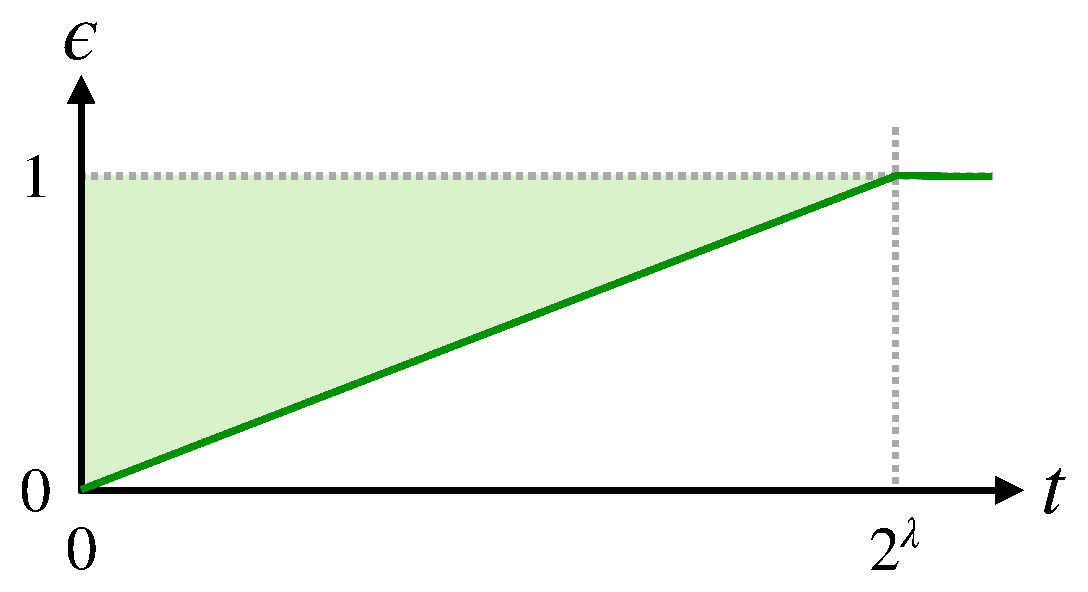
\includegraphics[width=\textwidth]{\FigureFolder/error-bounds-linear-growth}
  \caption{}
  \label{figure:error-bounds-linear-growth}
\end{subfigure}
\quad
\begin{subfigure}[b]{0.4\textwidth}
  \centering
  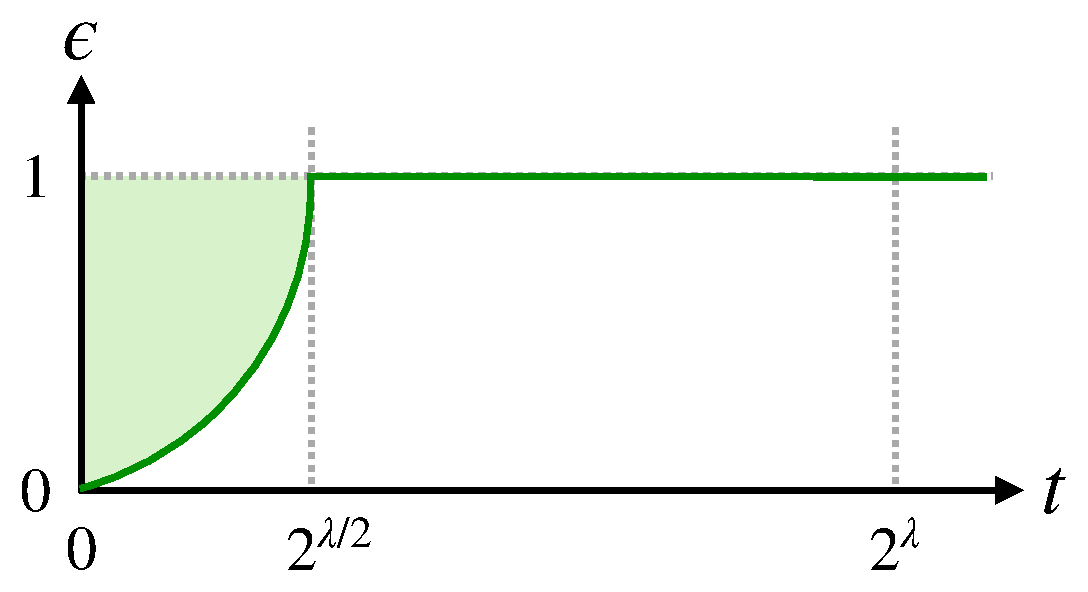
\includegraphics[width=\textwidth]{\FigureFolder/error-bounds-quadratic-growth}
  \caption{}
  \label{figure:error-bounds-quadratic-growth}
\end{subfigure}
\caption[Common error bound types.]{Common error bound types: $\ErrorBound(\SecurityParameter,\ResourceBound) = \ResourceBound/2^{\SecurityParameter}$ on the left and $\ErrorBound(\SecurityParameter,\ResourceBound) = \ResourceBound^2/2^{\SecurityParameter}$ on the right.}
\label{figure:error-bounds-growth-comparison}
\end{figure}

Typically, for every $\SecurityParameter \in \Naturals$, $\lim_{\ResourceBound \to \infty} \ErrorBound(\SecurityParameter,\ResourceBound)=1$, in other words, an adversary with enough resources can break the security guarantee of the given cryptographic primitive with probability $1$, regardless of the security parameter $\SecurityParameter$ used to instantiate the cryptographic primitive. Consider, for example, the case of a non-interactive argument in the ROM: for a given instance not in the language, an adversary can iterate over every possible argument string in search of an argument string that convinces the argument verifier. (As discussed in \Cref{section:lower-bound-on-argument-size}, this attack implies a lower bound on argument size of any non-trivial non-interactive argument.)

Therefore, any discussion of security must be limited to adversaries whose resources are bounded by an appropriate maximum bound $\ResourceBound_{\max}$. In other words, the goal is to set the security parameter $\SecurityParameter$ of the cryptographic primitive in order to achieve security only against adversaries whose resources are bounded by $\ResourceBound_{\max}$. Thus, we care about the values of the error function $\ErrorBound(\SecurityParameter,\ResourceBound)$ only for $\ResourceBound \leq \ResourceBound_{\max}$.

But what does \DoQuote{secure} mean? It is \emph{not} enough to know only a few values of $\ErrorBound(\SecurityParameter,\ResourceBound)$ for $\ResourceBound \leq t_{\max}$. For example, setting $\SecurityParameter=256$ for concreteness, we cannot conclude anything if we know that $\ErrorBound(256,2) \leq 2^{-127}$ and $\ErrorBound(256,2^{127}) \leq 2^{-1}$; indeed, it might be that $\ErrorBound(256,\ResourceBound) = 2^{-1}$ for every $\ResourceBound \in \{3,\dots,2^{127}\}$, which no definition should consider secure.

A reasonable answer would be to assess security by considering all values of $\ErrorBound(\SecurityParameter,\ResourceBound)$ on the interval $[\ResourceBound_{\max}] \DefineEqual \{1,\dots,\ResourceBound_{\max}\}$. However, this is not very informative: it is unclear how to compare the security achieved by cryptographic primitives with different error functions. For example, which of two error functions in \Cref{figure:error-bounds-two-curves} is \DoQuote{more secure}?

\begin{figure}[htp!]
\centering
\begin{subfigure}[b]{0.4\textwidth}
\centering
  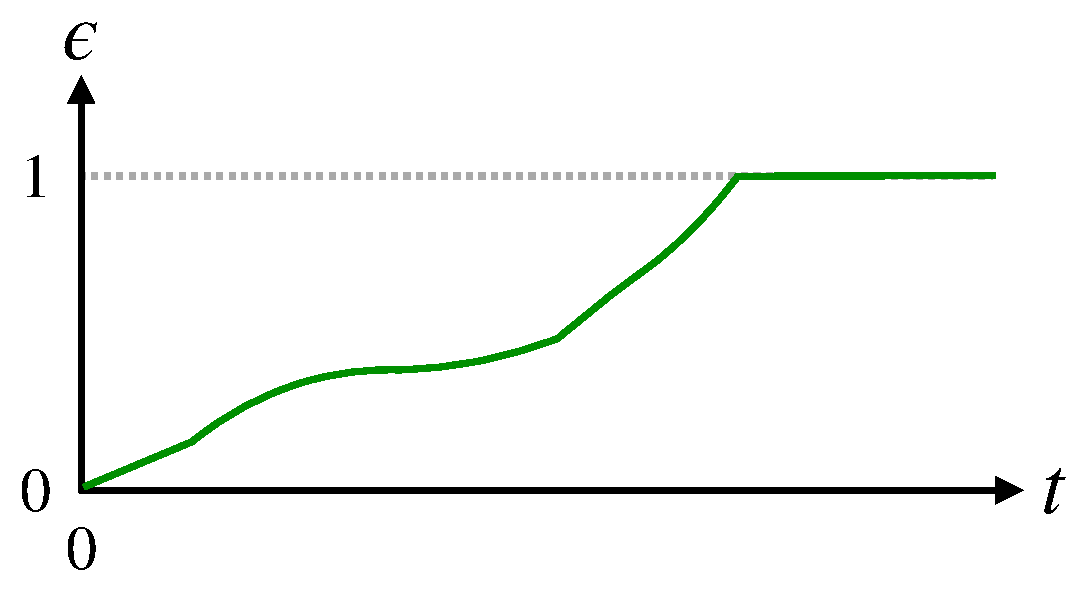
\includegraphics[width=\textwidth]{\FigureFolder/error-bounds-curve-1}
  \caption{}
  \label{figure:error-bounds-curve-1}
\end{subfigure}
\quad
\begin{subfigure}[b]{0.4\textwidth}
  \centering
  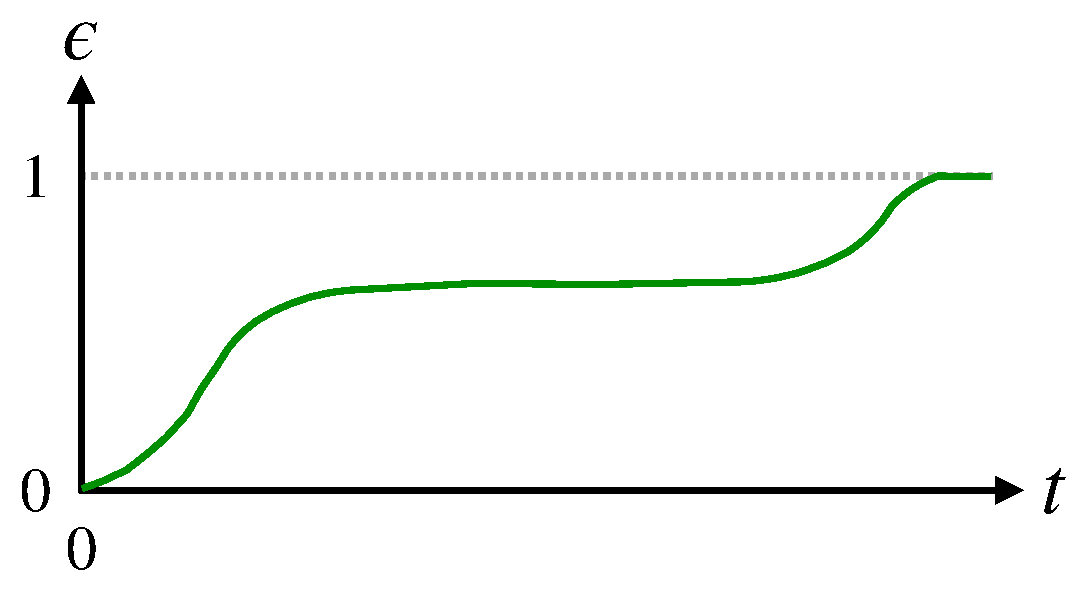
\includegraphics[width=\textwidth]{\FigureFolder/error-bounds-curve-2}
  \caption{}
  \label{figure:error-bounds-curve-2}
\end{subfigure}
\caption[Two different error bound functions.]{Two different error bound functions $\ErrorBound(\SecurityParameter,\ResourceBound)$. The left-side error bound is better for smaller values of $\ResourceBound$ while the right-side error bound is better for larger values of $\ResourceBound$. Neither is \DoQuote{better} than the other.}
\label{figure:error-bounds-two-curves}
\end{figure}

\parhead{Defining a security level}
An alternative answer is to distill from the error function $\ErrorBound$ a single number that captures the \DoQuote{security level} of a primitive. While it does not carry as much information as the error function $\ErrorBound$ itself, a single number is a more convenient way to convey and compare security of cryptographic primitives. Below we describe two approaches to define security level.
\begin{itemize}
  \item \emph{Worst-case security level.}
  A cryptographic primitive instantiated with security parameter $\SecurityParameter$ has \textbf{worst-case security level of $\SecurityLevel$ bits} if $\ErrorBound(\SecurityParameter,\ResourceBound) \leq 2^{-\SecurityLevel}$ for \emph{every} $\ResourceBound \in [2^{\SecurityLevel}]$. Since we assume that $\ErrorBound$ is non-decreasing in $\ResourceBound$, the condition is equivalent to $\ErrorBound(\SecurityParameter,2^{\SecurityLevel}) \leq 2^{-\SecurityLevel}$.
  \item \emph{Average-case security level.}
  A cryptographic primitive instantiated with security parameter $\SecurityParameter$ has \textbf{average-case security level of $\SecurityLevel$ bits} if $\ResourceBound/\ErrorBound(\SecurityParameter,\ResourceBound) \geq 2^{\SecurityLevel}$ for every $\ResourceBound \in [2^{\SecurityLevel}]$. The motivation behind this definition is that $\ResourceBound/\ErrorBound(\SecurityParameter,\ResourceBound)$ is the expected amount of resources for a successful attack: an attack with resources bounded by $\ResourceBound$ succeeds (at best) with probability $\ErrorBound(\SecurityParameter,\ResourceBound)$, so in expectation a successful attack takes $\ResourceBound/\ErrorBound(\SecurityParameter,\ResourceBound)$ resources.
\end{itemize}
If a cryptographic primitive has $\SecurityLevel$ bits of worst-case security then it has $\SecurityLevel$ bits of average-case security; indeed, for every $\ResourceBound \in \{1,\dots,2^{\SecurityLevel}\}$, $\ResourceBound/\ErrorBound(\SecurityParameter,\ResourceBound) \geq \ResourceBound 2^{\SecurityLevel} \geq 2^{\SecurityLevel}$. \Cref{figure:error-bounds-two-types-of-security-level} illustrates how this implication is straightforward to see visually.

Worst-case security is stronger than average-case security but the more stringent requirement translates to a larger security parameter, and in turn a more expensive instantiation. In practice it is rather common to settle for average-case security.

\begin{figure}[htp!]
\centering
\begin{subfigure}[b]{0.4\textwidth}
\centering
  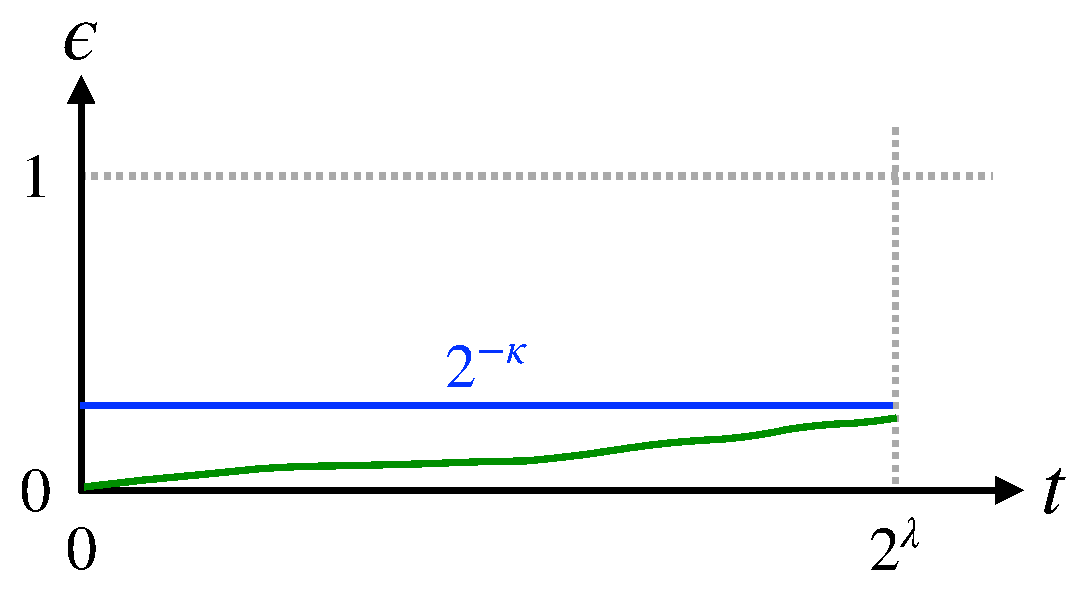
\includegraphics[width=\textwidth]{\FigureFolder/error-bounds-worst-case}
  \caption{}
  \label{figure:error-bounds-worst-case}
\end{subfigure}
\quad
\begin{subfigure}[b]{0.4\textwidth}
  \centering
  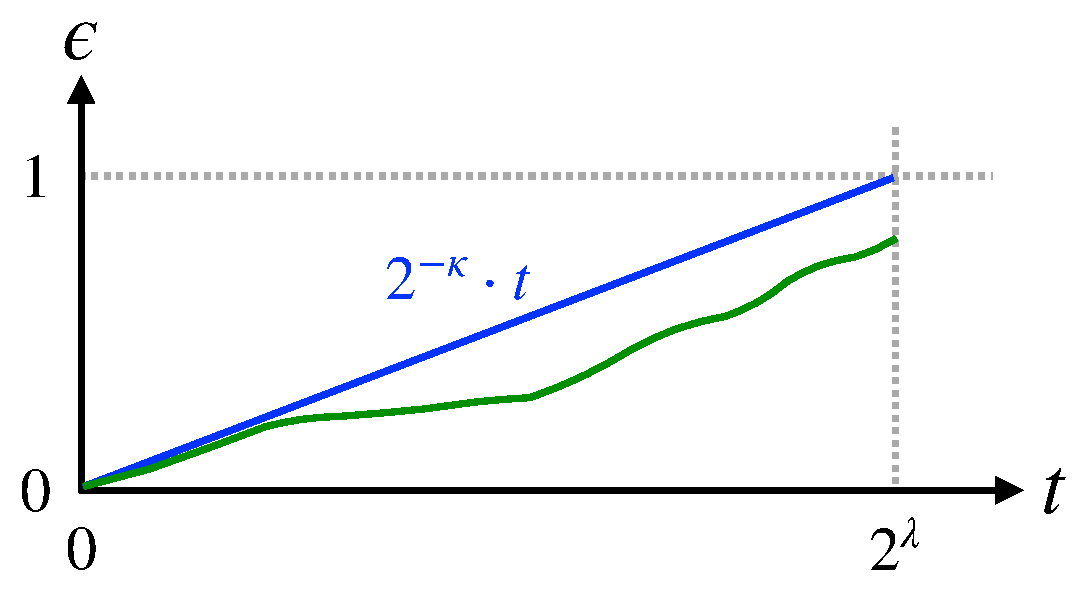
\includegraphics[width=\textwidth]{\FigureFolder/error-bounds-average-case}
  \caption{}
  \label{figure:error-bounds-average-case}
\end{subfigure}
\caption[Two definitions for security level.]{Diagrams showing the requirements for $\SecurityLevel$ bits of security according to the two definitions. The left-side diagram shows worst-case security: the error bound (green line) must not go above the horizontal (blue) line at height $2^{-\SecurityLevel}$, within the interval $[2^{\SecurityLevel}]$. The right-side diagram shows average-case security: the error bound (green line) must not go above the oblique (blue) line, within the interval $[2^{\SecurityLevel}]$.}
\label{figure:error-bounds-two-types-of-security-level}
\end{figure}

\parhead{Example: basic commitments}
Consider the basic commitment scheme $\CMSymbol \DefineEqual \CMConstructor{\ROOutputSize}{\CMMessageLength}{\CMSaltSize}$ described and analyzed in \Cref{chapter:basic-commitment}. Recall that $\ROOutputSize$ is the output size of the random oracle, $\CMMessageLength$ is the message length, and $\CMSaltSize$ is the salt size. We apply the above discussion to $\CMSymbol$.

First we discuss the binding property: by \Cref{lemma:cm-binding} the probability that a $\ROQueryBound$-query algorithm breaks the binding property of $\CMSymbol$ is at most $\CMBindingExpression{\ROOutputSize}{\ROQueryBound}$. We take the security parameter $\SecurityParameter$ to be $\ROOutputSize$ (the output size of the random oracle).
\begin{itemize}
  \item \emph{$\SecurityLevel$ bits of worst-case security.}
  If we set $\ROOutputSize=3\SecurityLevel-1$ then
\begin{equation*}
\forall\, \ROQueryBound \in [2^{\SecurityLevel}]\,,\;
\CMBindingExpression{\ROOutputSize}{\ROQueryBound}
\leq \frac{1}{2} \cdot \frac{(2^{\SecurityLevel})^2}{2^{\ROOutputSize}}
= \frac{2^{2\SecurityLevel}}{2^{3\SecurityLevel}}
= \frac{1}{2^{\SecurityLevel}}
\enspace.
\end{equation*}
  \item \emph{$\SecurityLevel$ bits of average-case security.}
  If we set $\ROOutputSize=2\SecurityLevel-1$ then
\begin{equation*}
\forall\, \ROQueryBound \in [2^{\SecurityLevel}]\,,\;
\frac{\ROQueryBound}{\CMBindingExpression{\ROOutputSize}{\ROQueryBound}}
= \frac{2 \cdot 2^{\ROOutputSize}}{\ROQueryBound}
\geq \frac{2 \cdot 2^{\ROOutputSize}}{2^{\SecurityLevel}}
= 2^{\SecurityLevel}
\enspace.
\end{equation*}
\end{itemize}
Therefore, for the binding property, to achieve (for example) $\SecurityLevel=128$ bits of worst-case security, we need output size $\ROOutputSize = 383$, and to achieve $\SecurityLevel=128$ bits of average-case security, we need output size $\ROOutputSize = 255$. More generally, the output size of the random oracle (here taken as the security parameter $\SecurityParameter$) for achieving worst-case security is about $1.5\times$ bigger compared to achieving average-case security.

Next, we discuss the extractability property. \Cref{lemma:cm-extractability} states that the error bound is the same as that of the binding property. This implies that the same computations as above hold for establishing security levels for the extractability property.

Finally, we discuss the hiding property: by \Cref{lemma:cm-hiding} the statistical distance between a real commitment and a simulated commitment is at most $\frac{\ROQueryBound}{2^{\CMSaltSize}}$ (for the case $\ROQueryBound<\infty$). We take the security parameter $\SecurityParameter$ to be $\CMSaltSize$ (the salt size).
\begin{itemize}
  \item \emph{$\SecurityLevel$ bits of worst-case security.}
  If we set $\CMSaltSize=2\SecurityLevel$ then
\begin{equation*}
\forall\, \ROQueryBound \in [2^{\SecurityLevel}]\,,\;
\frac{\ROQueryBound}{2^{\CMSaltSize}}
\leq \frac{2^{\SecurityLevel}}{2^{\CMSaltSize}}
= \frac{2^{\SecurityLevel}}{2^{2\SecurityLevel}}
= \frac{1}{2^{\SecurityLevel}}
\enspace.
\end{equation*}
  \item \emph{$\SecurityLevel$ bits of average-case security.}
  If we set $\CMSaltSize=\SecurityLevel$ then
\begin{equation*}
\forall\, \ROQueryBound \in [2^{\SecurityLevel}]\,,\;
\frac{\ROQueryBound}{\frac{\ROQueryBound}{2^{\CMSaltSize}}}
= 2^{\CMSaltSize}
= 2^{\SecurityLevel}
\enspace.
\end{equation*}
\end{itemize}
Therefore, for the hiding property, to achieve (for example) $\SecurityLevel=128$ bits of worst-case security we need salt size $\CMSaltSize = 256$ and to achieve $\SecurityLevel=128$ bits of average-case security we need salt size $\CMSaltSize = 128$. More generally, the salt size $\CMSaltSize$ for achieving worst-case security is $2\times$ bigger compared to achieving average-case security.

\parhead{Additional parameters}
A security definition may involve other parameters affecting the error bound (besides the adversary's resource bound $\ResourceBound$).

For example, this is the case for the multi-extractability property of $\CMSymbol$: by \Cref{lemma:cm-multi-extractability}, the probability that a $\ROQueryBound$-query algorithm breaks the multi-extractability property of the basic commitment $\CMSymbol$ is at most $\CMMultiExtractabilityExpression{\ROOutputSize}{\ROQueryBound}{\CMNumCommitments}$, where $\CMNumCommitments$ is the number of commitments. Taking the security parameter $\SecurityParameter$ to be the output size of the random oracle $\ROOutputSize$, the error bound is a function $\ErrorBound(\SecurityParameter,\ROQueryBound,\CMNumCommitments)$.

In general, the error bound for the security property may be a function $\ErrorBound(\SecurityParameter,\ResourceBound,\ParameterChoice)$ where $\ParameterChoice$ denotes some vector of parameters that specifies quantities that appear in the security definition. This affects how a security level is defined (and achieved).

We describe how to extend the definitions of security level to consider this more general case.

Denote by $\ParameterSet$ the set of parameters to consider for deriving the security level. The definitions below consider the worst-case choice of parameters within the set $\ParameterSet$.
\begin{itemize}
  \item \emph{Worst-case security level.}
  A cryptographic primitive instantiated with security parameter $\SecurityParameter$ has \textbf{worst-case security level of $\SecurityLevel$ bits} if $\max_{\ParameterChoice \in \ParameterSet} \{ \ErrorBound(\SecurityParameter,\ResourceBound,\ParameterChoice) \} \leq 2^{-\SecurityLevel}$ for every $\ResourceBound \in [2^{\SecurityLevel}]$.
  \item \emph{Average-case security level.}
  A cryptographic primitive instantiated with security parameter $\SecurityParameter$ has \textbf{average-case security level of $\SecurityLevel$ bits} if $\min_{\ParameterChoice \in \ParameterSet} \{ t/\ErrorBound(\SecurityParameter,\ResourceBound,\ParameterChoice) \} \geq 2^{\SecurityLevel}$ for every $\ResourceBound \in[2^{\SecurityLevel}]$.
\end{itemize}
We illustrate how to use these definitions by returning to the multi-extractability property of the basic commitment $\CMSymbol$ (captured by \Cref{lemma:cm-multi-extractability}). Here the number of commitments $\CMNumCommitments$ is the (single) additional parameter, and we set $\ParameterSet \DefineEqual [2^{40}]$, which means that we consider security against adversaries that output up to $2^{40}$ commitments (and make the minor assumption that $2^{40} \leq 2^{\SecurityLevel-1}$).
\begin{itemize}
  \item \emph{$\SecurityLevel$ bits of worst-case security.}
  If we set $\ROOutputSize=3\SecurityLevel$ then
\begin{equation*}
\forall\, \ROQueryBound \in [2^{\SecurityLevel}]\,,\;
\max_{\CMNumCommitments \in [2^{40}]} \left\{ \CMMultiExtractabilityExpression{\ROOutputSize}{\ROQueryBound}{\CMNumCommitments} \right\}
= \CMMultiExtractabilityExpression{\ROOutputSize}{\ROQueryBound}{2^{40}}
\leq \frac{2^{-1} \cdot (2^{\SecurityLevel})^2 + 2^{40} \cdot 2^{\SecurityLevel}}{2^{\ROOutputSize}}
\leq \frac{1}{2^{\SecurityLevel}}
\enspace.
\end{equation*}
  \item \emph{$\SecurityLevel$ bits of average-case security.}
  If we set $\ROOutputSize=2\SecurityLevel$ then
\begin{equation*}
\forall\, \ROQueryBound \in [2^{\SecurityLevel}]\,,\;
\min_{\CMNumCommitments \in [2^{40}]} \left\{\frac{\ROQueryBound}{\CMMultiExtractabilityExpression{\ROOutputSize}{\ROQueryBound}{\CMNumCommitments}} \right\}
= \frac{\ROQueryBound}{\CMMultiExtractabilityExpression{\ROOutputSize}{\ROQueryBound}{2^{40}}}
= \frac{2^{\ROOutputSize}}{\ROQueryBound/2 + 2^{40}}
\geq \frac{2^{\ROOutputSize}}{2^{\SecurityLevel-1} + 2^{40}}
\geq 2^{\SecurityLevel}
\enspace.
\end{equation*}
\end{itemize}
Therefore, for the multi-extractability property, to achieve (for example) $\SecurityLevel=128$ bits of worst-case security we need output size $\ROOutputSize = 384$ and to achieve $\SecurityLevel=128$ bits of average-case security we need output size $\ROOutputSize = 256$. In general, the output size of the random oracle (here the security parameter $\SecurityParameter$) for achieving worst-case security is $1.5\times$ bigger compared to achieving average-case security.


%%%%%%%%%%%%%%%%%%%%%%%%%%%%%%%%%%%%%%%%%%%%%%%%%%%%%%%%%%%%%%%%%%%%%%%%%%%%%%%
%%%%%%%%%%%%%%%%%%%%%%%%%%%%%%%%%%%%%%%%%%%%%%%%%%%%%%%%%%%%%%%%%%%%%%%%%%%%%%%
%%%%%%%%%%%%%%%%%%%%%%%%%%%%%%%%%%%%%%%%%%%%%%%%%%%%%%%%%%%%%%%%%%%%%%%%%%%%%%%
\section{Concrete security for argument systems}
\label{section:concrete-security-for-argument-systems}

We illustrate how to apply the ideas in \Cref{section:security-levels} to achieve (worst-case or average-case) security levels for non-interactive arguments in the ROM. In \Cref{section:concrete-security-for-micali}, we use the example of the Micali transformation (see \Cref{chapter:micali-transformation}), and in \Cref{section:concrete-security-for-bcs} the example of the BCS transformation (see \Cref{chapter:bcs-transformation}). Similar discussions are straightforward for other constructions studied in this book.

The security definitions for arguments in the ROM that we provide in \Cref{chapter:argument-definitions} and \Cref{chapter:narg-advanced} consider the simple setting where there is a single random oracle with output size $\ROOutputSize$, which can be identified as the security parameter $\SecurityParameter$. (That is, those definitions set $\SecurityParameter=\ROOutputSize$.)

More generally, as we discuss in \Cref{chapter:multiple-oracles-reduction}, the number of random oracles and their output sizes for an argument in the ROM are determined by an oracle configuration function $\ARGOracles$ that receives as input the security parameter $\SecurityParameter$ and instance size bound $\InstanceSize$ (and in this case, the argument prover and argument verifier implicitly receive $\SecurityParameter$ and $\InstanceSize$). For example, in the Micali transformation, there are two oracles: one with output size $\SecurityParameter$ and one with output size $\PCPRandomnessComplexity$ (the randomness complexity of the underlying PCP verifier used to construct the non-interactive argument). This leads to security definitions for soundness, knowledge soundness, and zero knowledge in the multi-oracle setting. While in \Cref{chapter:multiple-oracles-reduction}, we show how the multi-oracle setting can be derived from the single-oracle setting, in this chapter, it is simpler to directly consider the multi-oracle setting.

In addition, an argument in the ROM may have other parameters that must be set, possibly based on the security parameter $\SecurityParameter$; in particular, many constructions in this book additionally have a privacy parameter $\PrivacyParameter$ that affects (among other things) the zero-knowledge error. For example, in the Micali transformation, $\PrivacyParameter$ determines the salt size in the underlying Merkle commitment scheme and in the Fiat--Shamir query.

Each security property of an argument has a corresponding security level. Therefore, ensuring that the argument overall achieves a desired security level entails ensuring that each security property achieves that security level. Thus, for a given argument, we discuss, in turn, the relevant properties: soundness, knowledge soundness, and zero knowledge.

%%%%%%%%%%%%%%%%%%%%%%%%%%%%%%%%%%%%%%%%%%%%%%%%%%%%%%%%%%%%%%%%%%%%%%%%%%%%%%%
%%%%%%%%%%%%%%%%%%%%%%%%%%%%%%%%%%%%%%%%%%%%%%%%%%%%%%%%%%%%%%%%%%%%%%%%%%%%%%%
\subsection{Example: the Micali transformation}
\label{section:concrete-security-for-micali}

\parhead{Soundness (\Cref{definition:narg-adaptive-soundness-with-cnf})}
The error bound is a function $\ARGSoundnessError(\SecurityParameter,\ROQueryBound,\InstanceSize)$ that depends on the security parameter $\SecurityParameter$, query bound $\ROQueryBound$ for the adversary, and instance size bound $\InstanceSize$.

\Cref{theorem:micali-soundness} gives the following soundness error bound for the Micali transformation (under the minor parameter condition in the theorem):
\begin{equation*}
\ARGSoundnessError(\SecurityParameter,\ROQueryBound,\InstanceSize) \leq (\ROQueryBound +1) \cdot \PCPSoundnessError(\InstanceSize) + \MTMultiExtractabilityShortExpression{\SecurityParameter}{\ROQueryBound}
\enspace.
\end{equation*}
Suppose we are happy with $\InstanceSize \leq 2^{64}$ (instances of size up to $2^{64}$).
\begin{itemize}

  \item \emph{Worst-case security.}
  Suppose that the underlying PCP is set to have soundness error $\PCPSoundnessError$ such that $\max_{\InstanceSize \in [2^{64}]} \{ \PCPSoundnessError(\InstanceSize) \} = \PCPSoundnessError(2^{64}) \leq 2^{-2\SecurityLevel-2}$. Setting $\SecurityParameter=3\SecurityLevel+2$ suffices for $\SecurityLevel$ bits of worst-case security for the soundness property:
\begin{align*}
\forall\, \ROQueryBound \in [2^{\SecurityLevel}]\,,\;
&\max_{\InstanceSize \in [2^{64}]} \left\{ (\ROQueryBound +1) \cdot \PCPSoundnessError(\InstanceSize) + \MTMultiExtractabilityShortExpression{\SecurityParameter}{\ROQueryBound} \right\}
= (\ROQueryBound +1) \cdot \PCPSoundnessError(2^{64}) + \MTMultiExtractabilityShortExpression{\SecurityParameter}{\ROQueryBound} \\
&\leq (2^{\SecurityLevel} +1) \cdot \frac{1}{2^{2\SecurityLevel+2}} + \MTMultiExtractabilityShortExpression{\SecurityParameter}{(2^{\SecurityLevel})}
= \frac{2^{\SecurityLevel} +1}{2^{2\SecurityLevel+2}} + \frac{2^{2\SecurityLevel+1}}{2^{3\SecurityLevel+2}} \\
&\leq \frac{1}{2^{\SecurityLevel+1}}+\frac{1}{2^{\SecurityLevel+1}} = \frac{1}{2^{\SecurityLevel}}
\enspace.
\end{align*}

  \item \emph{Average-case security.}
  Suppose that the underlying PCP is set to have soundness error $\PCPSoundnessError$ such that $\max_{\InstanceSize \in [2^{64}]} \{ \PCPSoundnessError(\InstanceSize) \} = \PCPSoundnessError(2^{64}) \leq 2^{-\SecurityLevel-1}$. Setting $\SecurityParameter=2\SecurityLevel+3$ suffices for $\SecurityLevel$ bits of average-case security for the soundness property:
\begin{align*}
\forall\, \ROQueryBound \in [2^{\SecurityLevel}]\,,\;
&\min_{\InstanceSize \in [2^{64}]} \left\{ \frac{\ROQueryBound}{(\ROQueryBound +1) \cdot \PCPSoundnessError(\InstanceSize) + \MTMultiExtractabilityShortExpression{\SecurityParameter}{\ROQueryBound}} \right\}
= \frac{\ROQueryBound}{(\ROQueryBound +1) \cdot \PCPSoundnessError(2^{64}) + \MTMultiExtractabilityShortExpression{\SecurityParameter}{\ROQueryBound}} \\
&= \frac{2^{\SecurityParameter}}{(1+\ROQueryBound^{-1}) \cdot \PCPSoundnessError(2^{64}) \cdot 2^{\SecurityParameter} + 2 \cdot \ROQueryBound}
\geq \frac{2^{\SecurityParameter}}{(1+2^{-\SecurityLevel}) \cdot 2^{-\SecurityLevel-1} \cdot 2^{\SecurityParameter} + 2 \cdot 2^{\SecurityLevel}} \\
&= \frac{2^{2\SecurityLevel+3}}{(1+2^{-\SecurityLevel}) \cdot 2^{\SecurityLevel+2} + 2^{\SecurityLevel+1}}
\geq \frac{2^{2\SecurityLevel+3}}{3/2 \cdot 2^{\SecurityLevel+2} + 1/2 \cdot 2^{\SecurityLevel+2}}
= 2^{\SecurityLevel}
\enspace.
\end{align*}

\end{itemize}

\parhead{Knowledge soundness (\Cref{definition:adaptive-straightline-knowledge-soundness-with-cnf})}
We consider \emph{straightline} knowledge soundness, which applies to the Micali transformation (due to the knowledge soundness property of the underlying PCP). The error bound in this case is a function $\ARGKnowledgeError(\SecurityParameter,\ROQueryBound,\InstanceSize)$ that takes as input the same parameters as the error bound in the soundness case (which is a function $\ARGSoundnessError(\SecurityParameter,\ROQueryBound,\InstanceSize)$).

\Cref{theorem:micali-knowledge-soundness} gives the knowledge soundness error bound for the Micali transformation:
\begin{equation*}
\ARGKnowledgeError(\SecurityParameter,\ROQueryBound,\InstanceSize) \leq (\ROQueryBound +1) \cdot \PCPKnowledgeError(\InstanceSize) + \MTMultiExtractabilityShortExpression{\SecurityParameter}{\ROQueryBound}
\enspace.
\end{equation*}
This is the same expression as the soundness error, except that the PCP knowledge soundness error $\PCPKnowledgeError$ replaces the PCP soundness error $\PCPSoundnessError$. The same computations as above directly carry over, in particular showing how to set parameters to achieve, for the knowledge soundness property, $\SecurityLevel$ bits of worst-case security and $\SecurityLevel$ bits of average-case security.

\parhead{Zero knowledge (\Cref{definition:once-adaptive-zk-narg-with-cnf})}
The error bound for zero knowledge is a function $\ARGOAZKError(\SecurityParameter,\ROQueryBound,\InstanceSize)$ that depends on the security parameter $\SecurityParameter$, query bound $\ROQueryBound$ for the adversary, and instance size bound $\InstanceSize$. \Cref{theorem:micali-zero-knowledge} states that the zero-knowledge error bound for the Micali transformation is
\begin{equation*}
\ARGOAZKError(\SecurityParameter,\ROQueryBound,\InstanceSize) \leq \MicaliZKExpression
\end{equation*}
where:
\begin{itemize}[nolistsep]
  \item $\PCPZKError$ is the error bound for honest-verifier zero knowledge of the underlying PCP;
  \item $\MTZKProofError$ is the hiding error of the Merkle commitment scheme from \Cref{lemma:mt-privacy};
  \item $\PCPProofLength$ and $\PCPQueryComplexity$ are the proof length and query complexity of the underlying PCP; and
  \item $\PrivacyParameter$ is the privacy parameter used in the Micali transformation.
\end{itemize}
In turn, \Cref{remark:mtzk-plugging-in-root-hiding-bound} tells us that, if $\ROQueryBound<\infty$, $\MTZKProofError(\SecurityParameter,\PCPProofLength(\InstanceSize),\PrivacyParameter,\PCPQueryComplexity(\InstanceSize),\ROQueryBound) \leq \frac{\PCPQueryComplexity(\InstanceSize) \cdot \PCPProofLength(\InstanceSize) \cdot \ROQueryBound}{2^{\MTSaltSize}} + \frac{\PCPQueryComplexity(\InstanceSize) \cdot \PCPProofLength(\InstanceSize) \cdot \ROQueryBound}{2^{2\ROOutputSize}}$. Hence the zero-knowledge error bound becomes
\begin{equation*}
\PCPZKError(\InstanceSize)
+ \frac{\PCPQueryComplexity(\InstanceSize) \cdot \PCPProofLength(\InstanceSize) \cdot \ROQueryBound}{2^{\MTSaltSize}} + \frac{\PCPQueryComplexity(\InstanceSize) \cdot \PCPProofLength(\InstanceSize) \cdot \ROQueryBound}{2^{2\ROOutputSize}}
+ \frac{\ROQueryBound}{2^{\RandSaltSize}}
\enspace.
\end{equation*}
In turn, if we assume that $\MTSaltSize \leq 2\ROOutputSize$ (a minor condition that we will satisfy), the above is at most
\begin{equation*}
\PCPZKError(\InstanceSize)
+ \frac{2 \cdot \PCPQueryComplexity(\InstanceSize) \cdot \PCPProofLength(\InstanceSize) \cdot \ROQueryBound}{2^{\MTSaltSize}}
+ \frac{\ROQueryBound}{2^{\RandSaltSize}}
\enspace.
\end{equation*}
We take the security parameter $\SecurityParameter$ to be $\RandSaltSize$ (the privacy parameter). We take the (very conservative) upper bounds $\PCPQueryComplexity(\InstanceSize) \leq 2^{20}$ and $\PCPProofLength(\InstanceSize) \leq 2^{40}$.
\begin{itemize}

  \item \emph{Worst-case security.}
  Suppose that the underlying PCP is set to have zero-knowledge error $\max_{\InstanceSize \in [2^{64}]} \{ \PCPZKError(\InstanceSize) \} = \PCPZKError(2^{64}) \leq 2^{-\SecurityLevel-2}$. Setting $\PrivacyParameter = 2\SecurityLevel+63$ suffices for $\SecurityLevel$ bits of worst-case security for the zero-knowledge property:
\begin{align*}
\forall\, \ROQueryBound \in [2^{\SecurityLevel}]\,,\;
&\max_{\InstanceSize \in [2^{64}]} \left\{ \PCPZKError(\InstanceSize)
+\frac{2 \cdot \PCPQueryComplexity(\InstanceSize) \cdot \PCPProofLength(\InstanceSize) \cdot \ROQueryBound}{2^{\PrivacyParameter}}+\frac{\ROQueryBound}{2^{\PrivacyParameter}} \right\} \\
&= \PCPZKError(2^{64})
+\frac{2 \cdot \PCPQueryComplexity(2^{64}) \cdot \PCPProofLength(2^{64}) \cdot \ROQueryBound}{2^{\PrivacyParameter}}+\frac{\ROQueryBound}{2^{\PrivacyParameter}} \\
&\leq \frac{1}{2^{\SecurityLevel+2}} + \frac{2 \cdot 2^{20} \cdot 2^{40} \cdot 2^{\SecurityLevel}}{2^{\PrivacyParameter}} + \frac{2^{\SecurityLevel}}{2^{\PrivacyParameter}} \\
&= \frac{2^{\SecurityLevel + 61}}{2^{2\SecurityLevel+63}} + \frac{2^{\SecurityLevel + 61}}{2^{2\SecurityLevel+63}} + \frac{2^{\SecurityLevel}}{2^{2\SecurityLevel+63}} \leq \frac{1}{2^{\SecurityLevel}}
\enspace.
\end{align*}

  \item \emph{Average-case security.}
  Suppose that the underlying PCP is set to have zero-knowledge error $\max_{\InstanceSize \in [2^{64}]} \{ \PCPZKError(\InstanceSize) \} = \PCPZKError(2^{64}) \leq 2^{-\SecurityLevel-2}$. Setting $\PrivacyParameter = \SecurityLevel+63$ suffices for $\SecurityLevel$ bits of average-case security for the zero-knowledge property:
\begin{align*}
\forall\, \ROQueryBound \in [2^{\SecurityLevel}]\,,\;
&\min_{\InstanceSize \in [2^{64}]} \left\{ \frac{\ROQueryBound}{\PCPZKError(\InstanceSize)+\frac{2 \cdot \PCPQueryComplexity(\InstanceSize) \cdot \PCPProofLength(\InstanceSize) \cdot \ROQueryBound}{2^{\PrivacyParameter}}+\frac{\ROQueryBound}{2^{\PrivacyParameter}}} \right\} \\
&= \frac{\ROQueryBound}{\PCPZKError(2^{64})+\frac{2 \cdot \PCPQueryComplexity(2^{64}) \cdot \PCPProofLength(2^{64}) \cdot \ROQueryBound}{2^{\PrivacyParameter}}+\frac{\ROQueryBound}{2^{\PrivacyParameter}}} \\
&= \frac{\ROQueryBound \cdot 2^{\PrivacyParameter}}{\PCPZKError(2^{64}) \cdot 2^{\PrivacyParameter}+2 \cdot \PCPQueryComplexity(2^{64}) \cdot \PCPProofLength(2^{64}) \cdot \ROQueryBound +\ROQueryBound} \\
&= \frac{2^{\PrivacyParameter}}{\PCPZKError(2^{64}) \cdot 2^{\PrivacyParameter} \cdot \ROQueryBound^{-1} + 2 \cdot \PCPQueryComplexity(2^{64}) \cdot \PCPProofLength(2^{64}) + 1} \\
&\geq \frac{2^{\PrivacyParameter}}{2^{-\SecurityLevel-2} \cdot 2^{\PrivacyParameter} \cdot 1 + 2 \cdot 2^{20} \cdot 2^{40} +1} \\
&= \frac{2^{\SecurityLevel+63}}{2^{-\SecurityLevel-2} \cdot 2^{\SecurityLevel+63}+2 \cdot 2^{20} \cdot 2^{40} +1} \\
&= \frac{2^{\SecurityLevel+63}}{2^{61} + 2^{61} +1}
\geq 2^{\SecurityLevel}
\enspace.
\end{align*}

\end{itemize}

%%%%%%%%%%%%%%%%%%%%%%%%%%%%%%%%%%%%%%%%%%%%%%%%%%%%%%%%%%%%%%%%%%%%%%%%%%%%%%%
%%%%%%%%%%%%%%%%%%%%%%%%%%%%%%%%%%%%%%%%%%%%%%%%%%%%%%%%%%%%%%%%%%%%%%%%%%%%%%%
\subsection{Example: the BCS transformation}
\label{section:concrete-security-for-bcs}

\parhead{Soundness (\Cref{definition:narg-adaptive-soundness-with-cnf})}
The error bound is a function $\ARGSoundnessError(\SecurityParameter,\ROQueryBound,\InstanceSize)$ that depends on the security parameter $\SecurityParameter$, query bound $\ROQueryBound$ for the adversary, and instance size bound $\InstanceSize$.

\Cref{theorem:bcs-soundness} gives the following soundness error bound for the BCS transformation (under the minor parameter condition in the theorem):
\begin{equation*}
\ARGSoundnessError(\SecurityParameter,\ROQueryBound,\InstanceSize) \leq \IOPSRSoundnessError(\SecurityParameter+\RandSaltSize,\ROQueryBound,\InstanceSize) + \BCSSimplifiedError
\enspace.
\end{equation*}
Suppose we are happy with $\InstanceSize \leq 2^{64}$ (instances of size up to $2^{64}$).
\begin{itemize}

  \item \emph{Worst-case security.}
  Suppose that the underlying IOP is set to have state-restoration soundness error $\IOPSRSoundnessError$ such that, for every $\SecurityParameter,\RandSaltSize$ and every $\ROQueryBound \in [2^{\SecurityLevel}]$, $\max_{\InstanceSize \in [2^{64}]} \{ \IOPSRSoundnessError(\SecurityParameter+\RandSaltSize,\ROQueryBound,\InstanceSize) \} = \IOPSRSoundnessError(\SecurityParameter+\RandSaltSize,\ROQueryBound,2^{64}) \leq 2^{-\SecurityLevel-1}$. Setting $\SecurityParameter=3\SecurityLevel+2$ suffices for $\SecurityLevel$ bits of worst-case security for the soundness property:
\begin{align*}
\forall\, \ROQueryBound \in [2^{\SecurityLevel}]\,,\;
&\max_{\InstanceSize \in [2^{64}]} \left\{ \IOPSRSoundnessError(\SecurityParameter+\RandSaltSize,\ROQueryBound,\InstanceSize) + \MTMultiMultiExtractabilityShortExpression{\SecurityParameter}{\ROQueryBound} \right\}
= \IOPSRSoundnessError(\SecurityParameter+\RandSaltSize,\ROQueryBound,2^{64}) + \MTMultiMultiExtractabilityShortExpression{\SecurityParameter}{\ROQueryBound} \\
&\leq \frac{1}{2^{\SecurityLevel+1}} + \MTMultiMultiExtractabilityShortExpression{\SecurityParameter}{(2^{\SecurityLevel})}
= \frac{1}{2^{\SecurityLevel+1}} + \frac{2^{2\SecurityLevel+1}}{2^{3\SecurityLevel+2}} \\
&= \frac{1}{2^{\SecurityLevel+1}}+\frac{1}{2^{\SecurityLevel+1}} = \frac{1}{2^{\SecurityLevel}}
\enspace.
\end{align*}

  \item \emph{Average-case security.}
  Suppose that the underlying IOP is set to have state-restoration soundness error $\IOPSRSoundnessError$ such that, for every $\SecurityParameter,\RandSaltSize$ and every $\ROQueryBound \in [2^{\SecurityLevel}]$, $\max_{\InstanceSize \in [2^{64}]} \{ \IOPSRSoundnessError(\SecurityParameter+\RandSaltSize,\ROQueryBound,\InstanceSize) \} = \IOPSRSoundnessError(\SecurityParameter+\RandSaltSize,\ROQueryBound,2^{64}) \leq 2^{-\SecurityLevel-1}$. Setting $\SecurityParameter=2\SecurityLevel+2$ suffices for $\SecurityLevel$ bits of average-case security for the soundness property:
\begin{align*}
\forall\, \ROQueryBound \in [2^{\SecurityLevel}]\,,\;
&\min_{\InstanceSize \in [2^{64}]} \left\{ \frac{\ROQueryBound}{\IOPSRSoundnessError(\SecurityParameter+\RandSaltSize,\ROQueryBound,\InstanceSize) + \MTMultiMultiExtractabilityShortExpression{\SecurityParameter}{\ROQueryBound}} \right\}
= \frac{\ROQueryBound}{\IOPSRSoundnessError(\SecurityParameter+\RandSaltSize,\ROQueryBound,2^{64}) + \MTMultiMultiExtractabilityShortExpression{\SecurityParameter}{\ROQueryBound}} \\
&= \frac{2^{\SecurityParameter} \cdot \ROQueryBound}{\IOPSRSoundnessError(\SecurityParameter+\RandSaltSize,\ROQueryBound,2^{64}) \cdot 2^{\SecurityParameter} + 2 \cdot \ROQueryBound^2}
\geq \frac{2^{\SecurityParameter} \cdot \ROQueryBound}{2^{-\SecurityLevel-1} \cdot 2^{\SecurityParameter} + 2 \cdot \ROQueryBound^2} \\
& = \frac{2^{\SecurityParameter}}{2^{-\SecurityLevel-1} \cdot 2^{\SecurityParameter} \cdot \ROQueryBound^{-1} + 2 \cdot \ROQueryBound}
 \geq \frac{2^{\SecurityParameter}}{2^{-\SecurityLevel-1} \cdot 2^{\SecurityParameter} \cdot 1 + 2 \cdot 2^{\SecurityLevel}} \\
& = \frac{2^{2\SecurityLevel+2}}{2^{\SecurityLevel+1} + 2^{\SecurityLevel+1}}
= 2^{\SecurityLevel}
\enspace.
\end{align*}

\end{itemize}

\parhead{Knowledge soundness (\Cref{definition:adaptive-straightline-knowledge-soundness-with-cnf})}
We consider \emph{straightline} knowledge soundness, which applies for the BCS transformation whenever the underlying IOP satisfies \emph{straightline} state-restoration knowledge soundness (IOPs of practical interest usually satisfy this notion). The error bound in this case is a function $\ARGKnowledgeError(\SecurityParameter,\ROQueryBound,\InstanceSize)$ that takes as input the same parameters as the error bound in the soundness case (which is a function $\ARGSoundnessError(\SecurityParameter,\ROQueryBound,\InstanceSize)$).

\Cref{theorem:bcs-knowledge-soundness} gives the knowledge soundness error bound for the BCS transformation:
\begin{equation*}
\ARGKnowledgeError(\SecurityParameter,\ROQueryBound,\InstanceSize) \leq \IOPSRKnowledgeError(\SecurityParameter+\RandSaltSize,\ROQueryBound,\InstanceSize) + \BCSSimplifiedError
\enspace.
\end{equation*}
This is the same expression as the soundness error, except that the IOP state-restoration knowledge soundness error $\IOPSRKnowledgeError$ replaces the IOP state-restoration soundness error $\IOPSRSoundnessError$. The same computations as above directly carry over, in particular showing how to set parameters to achieve, for the knowledge soundness property, $\SecurityLevel$ bits of worst-case security and $\SecurityLevel$ bits of average-case security.

\parhead{Zero knowledge (\Cref{definition:once-adaptive-zk-narg-with-cnf})}
The error bound for zero knowledge is a function $\ARGOAZKError(\SecurityParameter,\ROQueryBound,\InstanceSize)$ that depends on the security parameter $\SecurityParameter$, query bound $\ROQueryBound$ for the adversary, and instance size bound $\InstanceSize$. \Cref{theorem:bcs-zero-knowledge} states that the zero-knowledge error bound for the BCS transformation is
\begin{equation*}
\ARGOAZKError(\SecurityParameter,\ROQueryBound,\InstanceSize) \leq \BCSZKExpression
\end{equation*}
where:
\begin{itemize}[nolistsep]
  \item $\IOPZKError$ is the error bound for honest-verifier zero knowledge of the underlying IOP;
  \item $\MTZKProofError$ is the hiding error of the Merkle commitment scheme from \Cref{lemma:mt-privacy};
  \item $\IOPProofLength$ and $\IOPQueryComplexity$ are the proof length and query complexity of the underlying IOP; and
  \item $\PrivacyParameter$ is the privacy parameter used in the BCS transformation.
\end{itemize}
This is the same error bound as the Micali transformation, except that $\IOPZKError$ replaces $\PCPZKError$. Therefore, we obtain analogous conclusions below because the same simplifications and derivations apply (which we omit). We similarly take the security parameter $\SecurityParameter$ to be $\RandSaltSize$ (the privacy parameter) and take the (very conservative) upper bounds $\IOPQueryComplexity(\InstanceSize) \leq 2^{20}$ and $\IOPProofLength(\InstanceSize) \leq 2^{40}$.
\begin{itemize}

  \item \emph{Worst-case security.}
  Suppose that the underlying IOP is set to have zero-knowledge error $\max_{\InstanceSize \in [2^{64}]} \{ \IOPZKError(\InstanceSize) \} = \IOPZKError(2^{64}) \leq 2^{-\SecurityLevel-2}$. Setting $\PrivacyParameter = 2\SecurityLevel+63$ suffices for $\SecurityLevel$ bits of worst-case security for the zero-knowledge property:
\begin{equation*}
\forall\, \ROQueryBound \in [2^{\SecurityLevel}]\,,\;
\max_{\InstanceSize \in [2^{64}]} \left\{ \IOPZKError(\InstanceSize)
+\frac{2 \cdot \IOPQueryComplexity(\InstanceSize) \cdot \IOPProofLength(\InstanceSize) \cdot \ROQueryBound}{2^{\PrivacyParameter}}+\frac{\ROQueryBound}{2^{\PrivacyParameter}} \right\} \\
\leq \frac{1}{2^{\SecurityLevel}}
\enspace.
\end{equation*}

  \item \emph{Average-case security.}
  Suppose that the underlying IOP is set to have zero-knowledge error $\max_{\InstanceSize \in [2^{64}]} \{ \IOPZKError(\InstanceSize) \} = \IOPZKError(2^{64}) \leq 2^{-\SecurityLevel-2}$. Setting $\PrivacyParameter = \SecurityLevel+63$ suffices for $\SecurityLevel$ bits of average-case security for the zero-knowledge property:
\begin{equation*}
\forall\, \ROQueryBound \in [2^{\SecurityLevel}]\,,\;
\min_{\InstanceSize \in [2^{64}]} \left\{ \frac{\ROQueryBound}{\IOPZKError(\InstanceSize)+\frac{2 \cdot \IOPQueryComplexity(\InstanceSize) \cdot \IOPProofLength(\InstanceSize) \cdot \ROQueryBound}{2^{\PrivacyParameter}}+\frac{\ROQueryBound}{2^{\PrivacyParameter}}} \right\}
\geq 2^{\SecurityLevel}
\enspace.
\end{equation*}

\end{itemize}


%%%%%%%%%%%%%%%%%%%%%%%%%%%%%%%%%%%%%%%%%%%%%%%%%%%%%%%%%%%%%%%%%%%%%%%%%%%%%%%
%%%%%%%%%%%%%%%%%%%%%%%%%%%%%%%%%%%%%%%%%%%%%%%%%%%%%%%%%%%%%%%%%%%%%%%%%%%%%%%
%%%%%%%%%%%%%%%%%%%%%%%%%%%%%%%%%%%%%%%%%%%%%%%%%%%%%%%%%%%%%%%%%%%%%%%%%%%%%%%
%%%%%%%%%%%%%%%%%%%%%%%%%%%%%%%%%%%%%%%%%%%%%%%%%%%%%%%%%%%%%%%%%%%%%%%%%%%%%%%
\chapter{Merkle commitment scheme optimizations}
\label{chapter:mt-optimizations}

We discuss two optimizations of the Merkle commitment scheme $\MTSymbol$ from \Cref{chapter:merkle-commitment} that are often used in practice. In \Cref{section:any-message-length}, we discuss how to support any message length without padding. In \Cref{section:compressing-opening-proof}, we discuss \emph{path pruning}, a method to reduce the size of Merkle opening proofs that authenticate multiple locations of the committed message vector.

%%%%%%%%%%%%%%%%%%%%%%%%%%%%%%%%%%%%%%%%%%%%%%%%%%%%%%%%%%%%%%%%%%%%%%%%%%%%%%%
%%%%%%%%%%%%%%%%%%%%%%%%%%%%%%%%%%%%%%%%%%%%%%%%%%%%%%%%%%%%%%%%%%%%%%%%%%%%%%%
%%%%%%%%%%%%%%%%%%%%%%%%%%%%%%%%%%%%%%%%%%%%%%%%%%%%%%%%%%%%%%%%%%%%%%%%%%%%%%%
\section{Any message length}
\label{section:any-message-length}

The description of the Merkle commitment scheme $\MTSymbol$ in \Cref{chapter:merkle-commitment} involves a binary tree over $\MTMessageLength$ leaves, where $\MTMessageLength$ is the number of entries in the message vector. For simplicity, $\MTMessageLength$ was assumed to be a power of $2$. In general, though, $\MTMessageLength$ need not be a power of $2$. Here, we discuss how to handle messages with any message length $\MTMessageLength$.

As noted in \Cref{remark:mt-any-message-length}, one option is to pad the message with dummy values (an arbitrary symbol from the alphabet $\MTAlphabet$) until the padded message length reaches a power of $2$; this, at most, doubles the length relative to the original (unpadded) message. All security analyses of $\MTSymbol$ in \Cref{chapter:merkle-commitment} hold for the padded message, and in particular for the original (unpadded) message.

While padding is not expensive, cheaper solutions are used in practice.

The definition of a Merkle commitment scheme in \Cref{section:merkle-commitment-definition} straightforwardly extends to work with \emph{any} tree, not just with a perfect binary tree (whose number of leaves is a power of $2$). The number of leaves of the tree determines the message length, and the \DoQuote{shape} of the tree affects  efficiency and security properties. Therefore, in order to support messages of arbitrary length, it suffices to define a family of trees $(\MTGraph_{\MTMessageLength})_{\MTMessageLength \in \Naturals}$ where $\MTGraph_{\MTMessageLength}$ has precisely $\MTMessageLength$ leaves.

We make the above discussion precise in two steps. First, we state the generalized definition of a Merkle commitment scheme for any given tree $\MTGraph_{\MTMessageLength}$ with $\MTMessageLength$ leaves and comment on its efficiency and security. Then, we describe a family of binary trees $(\MTGraph_{\MTMessageLength})_{\MTMessageLength \in \Naturals}$ that is often used in practice. Combining these two steps yields efficient and secure Merkle commitment schemes for any message length.

\parhead{(1) Merkle commitment scheme from any tree}
Let $\MTGraph_{\MTMessageLength} = (\MTVertexSet_{\MTMessageLength},\MTEdgeSet_{\MTMessageLength})$ be a (rooted) tree with $\MTMessageLength$ leaves. We use the tree $\MTGraph_{\MTMessageLength}$ to describe a \emph{generalized Merkle commitment scheme} $\MTSymbol \DefineEqual \MTConstructor{\ROOutputSize}{\MTAlphabet}{\MTGraph_{\MTMessageLength}}{\MTSaltSize}$ for messages of length $\MTMessageLength$; note that the tree $\MTGraph_{\MTMessageLength}$ is arbitrary and, in particular, need not be binary or balanced. We begin with some graph notation associated with the tree $\MTGraph_{\MTMessageLength}$; this generalizes the notation in \Cref{definition:mt-paths} for perfect binary trees to the case of any tree.

\begin{definition}
\label{definition:notation-for-arbitrary-tree}
We make the following notational definitions for $\MTGraph_{\MTMessageLength}$:
\begin{itemize}[nolistsep]
  \item The \defemph{root vertex} of $\MTGraph_{\MTMessageLength}$ is the vertex denoted $\MTGraphVertex_{0}$.
  \item The \defemph{leaf vertices} of $\MTGraph_{\MTMessageLength}$ are the vertices denoted $(\MTGraphLeaf_{\MTMessageIndex})_{\MTMessageIndex \in [\MTMessageLength]}$.
  \item The \defemph{path} of the $\MTMessageIndex$-th leaf vertex $\MTGraphLeaf_{\MTMessageIndex}$, denoted $\MTPath(\MTMessageIndex)$, is the list of vertices on the (unique) path from $\MTGraphLeaf_{\MTMessageIndex}$ to the root vertex $\MTGraphVertex_{0}$. (The path includes the leaf vertex and the root vertex.)
  \item The \defemph{copath} of the $\MTMessageIndex$-th leaf vertex $\MTGraphLeaf_{\MTMessageIndex}$, denoted $\MTCoPath(\MTMessageIndex)$, is a list of lists that contains, for each vertex $\MTGraphVertex$ in $\MTPath(\MTMessageIndex)$, the list of siblings of $\MTGraphVertex$. (The root vertex has no siblings, so its empty list of siblings is omitted from $\MTCoPath(\MTMessageIndex)$.)
  \item The \defemph{depth} of the leaf vertex $\MTGraphLeaf_{\MTMessageIndex}$ is $\MTDepth_{\MTMessageIndex} \DefineEqual \Cardinality{\MTPath(\MTMessageIndex)}-1$ (the minus $1$ appears because the root vertex is defined to have depth $0$ rather than depth $1$). Different leaves may have different depths. The \defemph{depth of the tree} is $\MTDepth \DefineEqual \max_{\MTMessageIndex \in [\MTMessageLength]} \MTDepth_{\MTMessageIndex}$.
\end{itemize}
\end{definition}

We describe each of the algorithms in the generalized Merkle commitment scheme
\begin{equation*}
\MTSymbol = (\MTCommit,\MTOpen,\MTCheck)
\end{equation*}
based on the (rooted) tree $\MTGraph_{\MTMessageLength}$.
\begin{itemize}
  \item $\MTCommit^{\ROFunction}(\MTMessageVector) \to (\MTCommitment,\MTTrapdoor)$
  \begin{enumerate}[nolistsep]
    \item For each message location $\MTMessageIndex = 1,\dots,\MTMessageLength$:
    \begin{itemize}[nolistsep]
      \item sample a salt $\MTSaltString_{\MTMessageIndex} \in \Bits^{\MTSaltSize}$;
      \item compute the (hiding) commitment $\MTVertexLabel_{\MTGraphLeaf_{\MTMessageIndex}} \DefineEqual \ROFunction(\MTMessageVector[\MTMessageIndex],\MTSaltString_{\MTMessageIndex}) \in \Bits^{\ROOutputSize}$.
    \end{itemize}
    \item Label the leaves of $\MTGraph_{\MTMessageLength}$ with $(\MTVertexLabel_{\MTGraphLeaf_{\MTMessageIndex}})_{\MTMessageIndex \in [\MTMessageLength]}$. Then label each unlabeled vertex $\MTGraphVertex \in \MTVertexSet$ as follows: if all children $\MTGraphVertex^{1},\dots,\MTGraphVertex^{\MTArity}$ of $\MTGraphVertex$ are already labeled, then set the label of $\MTGraphVertex$ to be
\begin{equation*}
\MTVertexLabel_{\MTGraphVertex} \DefineEqual \ROFunction(\MTVertexLabel_{\MTGraphVertex^{1}},\dots,\MTVertexLabel_{\MTGraphVertex^{\MTArity}}) \in \Bits^{\ROOutputSize}
\enspace.
\end{equation*}
    \item Set the Merkle commitment $\MTCommitment$ to be the label of the root vertex $\MTGraphVertex_{0}$ of $\MTGraph_{\MTMessageLength}$.
    \item Set the salts $\MTSaltStrings \DefineEqual (\MTSaltString_{\MTMessageIndex})_{\MTMessageIndex \in [\MTMessageLength]}$.
    \item Set the commitments $\MTVertexLabels \DefineEqual (\MTVertexLabel_{\MTGraphVertex})_{\MTGraphVertex \in \MTVertexSet_{\MTMessageLength}}$.
    \item Set the opening trapdoor $\MTTrapdoor \DefineEqual (\MTSaltStrings,\MTVertexLabels)$.
    \item Output $(\MTCommitment,\MTTrapdoor)$.
  \end{enumerate}
  \item $\MTOpen^{\ROFunction}(\MTTrapdoor, \MTMessageIndexSet) \to \MTProof$.
  \begin{enumerate}[nolistsep]
    \item For every $\MTMessageIndex \in \MTMessageIndexSet$, set the authentication path for location $\MTMessageIndex$:
\begin{equation}
\label{equation:generalized-mt-authpath-structure}
\MTAuthPath_{\MTMessageIndex}
\DefineEqual
\big(
  \MTSaltString_{\MTMessageIndex}
  ,
  (\MTVertexLabel_{\MTGraphVertex})_{\MTGraphVertex \in \MTCoPath(\MTMessageIndex)}
\big)
\enspace.
\end{equation}
    \item Output the opening proof $\MTProof \DefineEqual (\MTAuthPath_{\MTMessageIndex})_{\MTMessageIndex \in \MTMessageIndexSet}$.
  \end{enumerate}
  \item $\MTCheck^{\ROFunction}(\MTCommitment,\MTMessageIndexSet,\MTMessageSubVector,\MTProof) \to b$.
  \begin{enumerate}[nolistsep]
    \item Parse $\MTProof$ as $(\MTAuthPath_{\MTMessageIndex})_{\MTMessageIndex \in \MTMessageIndexSet}$.
    \item For every $\MTMessageIndex \in \MTMessageIndexSet$, check that $\MTAuthPath_{\MTMessageIndex}=\big(\MTSaltString_{\MTMessageIndex},(\MTVertexLabel_{\MTGraphVertex})_{\MTGraphVertex \in \MTCoPath(\MTMessageIndex)}\big)$ authenticates the value $\MTMessageSubVector[\MTMessageIndex] \in \MTAlphabet$ as the $\MTMessageIndex$-th opening relative to the Merkle commitment $\MTCommitment \in \Bits^{\ROOutputSize}$ by computing $(\MTVertexLabel_{\MTGraphVertex})_{\MTGraphVertex \in \MTPath(\MTMessageIndex)}$:
    \begin{enumerate}[nolistsep]
      \item compute the commitment $\MTVertexLabel_{\MTGraphLeaf_{\MTMessageIndex}} \DefineEqual \ROFunction(\MTMessageSubVector[\MTMessageIndex],\MTSaltString_{\MTMessageIndex})$;
      \item for each $\MTGraphVertex \in \MTPath(\MTMessageIndex)\setminus \{\MTGraphLeaf_{\MTMessageIndex}\}$, letting $\MTGraphVertex^{1},\dots,\MTGraphVertex^{\MTArity}$ be the children of $\MTGraphVertex$ (one of which is in $\MTPath(\MTMessageIndex)$ and all others are in $\MTCoPath(\MTMessageIndex)$), set the commitment
\begin{equation*}
\MTVertexLabel_{\MTGraphVertex} \DefineEqual \ROFunction(\MTVertexLabel_{\MTGraphVertex^{1}},\dots,\MTVertexLabel_{\MTGraphVertex^{\MTArity}}) \in \Bits^{\ROOutputSize}
\enspace.
\end{equation*}
      \item check that $\MTCommitment = \MTVertexLabel_{\MTGraphVertex_{0}}$ where $\MTGraphVertex_{0}$ is the root vertex of $\MTGraph_{\MTMessageLength}$.
    \end{enumerate}
  \end{enumerate}
\end{itemize}
We discuss the efficiency of each algorithm.
\begin{itemize}

  \item The algorithm $\MTCommit$ makes $\MTMessageLength$ queries of size $\log\Cardinality{\MTAlphabet}+\MTSaltSize$, and $\Cardinality{\MTVertexSet_{\MTMessageLength}} - \MTMessageLength$ queries of varying size (the size is a multiple of $\ROOutputSize$ that depends on the number of children of a given vertex). The output Merkle commitment $\MTCommitment$ has size $\ROOutputSize$ and opening trapdoor $\MTTrapdoor$ has size $\MTSaltSize \MTMessageLength + \Cardinality{\MTVertexSet_{\MTMessageLength}} \cdot \ROOutputSize$.

  \item The algorithm $\MTOpen$ makes no oracle calls, and simply includes in the opening proof an authentication path for each index in the set $\MTMessageIndexSet$. An authentication path for location $\MTMessageIndex \in \MTMessageIndexSet$ has size $\MTSaltSize + \Cardinality{\MTCoPath(\MTMessageIndex)} \cdot \ROOutputSize$, since it includes the salt and a hash per vertex in the copath.

  \item The algorithm $\MTCheck$, for each location $\MTMessageIndex \in \MTMessageIndexSet$, makes a single query of size $\log\Cardinality{\MTAlphabet}+\MTSaltSize$ and $\Cardinality{\MTPath(\MTMessageIndex)}-1$ queries of varying size (the size is a multiple of $\ROOutputSize$ that depends on the number of children of a given vertex).

\end{itemize}
We do not prove the security properties associated to the generalized Merkle commitment scheme. Instead, we comment on how the security properties differ from the case of Merkle commitment schemes based on perfect binary trees that we study in detail in \Cref{chapter:merkle-commitment}.
\begin{itemize}

  \item \emph{Collision lemma.}
  \Cref{lemma:mt-colliding-paths} and its special case \Cref{lemma:simple-mt-colliding-paths} hold as stated for the generalized Merkle commitment scheme. Extending the proofs of those lemmas (which are for a perfect binary tree) to work for an arbitrary tree $\MTGraph_{\MTMessageLength}$ is straightforward.

  \item \emph{Binding.}
  \Cref{lemma:mt-binding} holds as stated for the generalized Merkle commitment scheme, with $\MTDepth$ now referring to the depth of the tree $\MTGraph_{\MTMessageLength}$. The analysis carries over essentially with no changes. Worth remarking here is that the upper bound $\Pr[\Event \land \Negate{\CollisionEvent}]
\leq \frac{(\MTDepth+1)^2}{2^{\ROOutputSize}}$ continues to hold because it is still true that $\Cardinality{\ROHonestTrace_{0}},\Cardinality{\ROHonestTrace_{1}} \leq \MTDepth+1$. Indeed, $\Cardinality{\ROHonestTrace_{0}},\Cardinality{\ROHonestTrace_{1}}$ are both at most $\MTDepth_{\MTMessageIndex}+1$ ($\MTMessageIndex$ is the minimal index in $\MTMessageIndexSet_{0} \cap \MTMessageIndexSet_{1}$ such that $\MTMessageSubVector_{0}[\MTMessageIndex] \neq \MTMessageSubVector_{1}[\MTMessageIndex]$); moreover, $\MTDepth_{\MTMessageIndex}+1 \leq \MTDepth+1$.

  \item \emph{Extractability.}
  \Cref{lemma:mt-extractability} (single extraction), \Cref{lemma:mt-multi-extractability} (multi-extraction), and \Cref{lemma:mt-multi-configuration-multi-extractability} (multi-extraction across multiple configurations) hold as stated for the generalized Merkle commitment scheme, with $\MTDepth$ now referring to the depth of the tree $\MTGraph_{\MTMessageLength}$. These extensions are also straightforward.

First, the Merkle commitment extractor $\MTExtractor$ (\Cref{construction:mt-extractor}) directly extends to work for the tree $\MTGraph_{\MTMessageLength}$; the main difference is that, when considering a query-answer pair $(\ROQuery,\ROAnswer) \in \MTInternalQueries$ in the main loop, the query $\ROQuery$ should be parsed in multiple blocks, depending on the arity of the vertex under consideration (in the case of a perfect binary tree, the arity is always two). Second, the analysis of \Cref{lemma:mt-extractability} carries over essentially with no changes, with the one remark that the size of the query-answer trace $\ROHonestTrace_{\MTMessageIndex}$ is now at most $\MTDepth_{\MTMessageIndex}+1$, which in turn is at most $\MTDepth+1$. A similar consideration holds for carrying over the analysis of \Cref{lemma:mt-multi-extractability,lemma:mt-multi-configuration-multi-extractability}.

  \item \emph{Hiding.}
  We discuss separately the two hiding lemmas. Here it is convenient to assume that \emph{every internal vertex of $\MTGraph_{\MTMessageLength}$ (including the root vertex) has at least two children}; this is essentially without loss of generality because there is no reason for an internal vertex to have a single child (that vertex can be replaced by its child).

  \Cref{lemma:mt-root-hiding} holds as stated for the generalized Merkle commitment scheme. First we discuss the case of $\ROQueryBound=\infty$. The analysis of this case directly carries over to show the bound
\begin{equation*}
\MTMessageLength \cdot \CMHidingError(\ROOutputSize,\MTSaltSize,\infty)
+
\sum_{\MTGraphVertex \in \MTVertexSet_{\MTMessageLength} \setminus \{\MTGraphLeaf_{\MTMessageIndex}\}_{\MTMessageIndex \in [\MTMessageLength]}}
\CMHidingError((\MTArity_{\MTGraphVertex}-1) \cdot \ROOutputSize,\ROOutputSize,\infty)
\end{equation*}
where $\MTArity_{\MTGraphVertex}$ is the number of children of the vertex $\MTGraphVertex$. The second term can be bounded by $\MTMessageLength \cdot \CMHidingError(\ROOutputSize,\ROOutputSize,\infty)$ because $\Cardinality{\MTVertexSet_{\MTMessageLength} \setminus \{\MTGraphLeaf_{\MTMessageIndex}\}_{\MTMessageIndex \in [\MTMessageLength]}} \leq \MTMessageLength$ (the number of non-leaf vertices in $\MTVertexSet_{\MTMessageLength}$ is at most $\MTMessageLength$ and $\CMHidingError((\MTArity_{\MTGraphVertex}-1) \cdot \ROOutputSize,\ROOutputSize,\infty) \leq \CMHidingError(\ROOutputSize,\ROOutputSize,\infty)$ (reducing the salt size from $(\MTArity_{\MTGraphVertex}-1) \cdot \ROOutputSize$ to $\ROOutputSize$ does not decrease the hiding error). Next we discuss the case of $\ROQueryBound < \infty$. The analysis of this case directly carries over to show the bound
\begin{equation*}
\frac{\MTMessageLength \cdot \ROQueryBound}{2^{\MTSaltSize}}
+
\sum_{\MTGraphVertex \in \MTVertexSet_{\MTMessageLength} \setminus \{\MTGraphLeaf_{\MTMessageIndex}\}_{\MTMessageIndex \in [\MTMessageLength]}}
\frac{\ROQueryBound}{2^{\MTArity_{\MTGraphVertex} \ROOutputSize}}
\end{equation*}
where $\MTArity_{\MTGraphVertex}$ is the number of children of the vertex $\MTGraphVertex$. The second term can be bounded by $\frac{\MTMessageLength \cdot \ROQueryBound}{2^{2\ROOutputSize}}$ because $\Cardinality{\MTVertexSet_{\MTMessageLength} \setminus \{\MTGraphLeaf_{\MTMessageIndex}\}_{\MTMessageIndex \in [\MTMessageLength]}} \leq \MTMessageLength$ (as above) and $\MTArity_{\MTGraphVertex} \geq 2$ (the arity of an internal vertex is at least two).

\Cref{lemma:mt-privacy} holds for the generalized Merkle commitment scheme but with a similar expression for the simulation error. Define $\MTZKRootError(\ROOutputSize,\MTGraph,\MTSaltSize,\ROQueryBound)$ to be the error from the generalization of \Cref{lemma:mt-root-hiding} for a given (rooted) tree $\MTGraph$ (not necessarily equal to $\MTGraph_{\MTMessageLength}$).
\begin{itemize}[nolistsep]
  \item If $\MTMessageIndexSetSize=0$ then the upper bound is (trivially) $\MTZKProofError(\ROOutputSize,\MTMessageLength,\MTSaltSize,\MTMessageIndexSetSize,\ROQueryBound) \DefineEqual \MTZKRootError(\ROOutputSize,\MTGraph_{\MTMessageLength},\MTSaltSize,\ROQueryBound)$.
  \item If $\MTMessageIndexSetSize>0$ then the upper bound is
\begin{equation*}
\MTZKProofError(\ROOutputSize,\MTMessageLength,\MTSaltSize,\MTMessageIndexSetSize,\ROQueryBound)
\DefineEqual
\max_{\MTMessageIndexSet \in \binom{[\MTMessageLength]}{\MTMessageIndexSetSize}}
\sum_{\MTGraphVertex \in \MTCoPathOptVertexSet} \MTZKRootError(\ROOutputSize,\MTGraph_{\MTMessageLength}[\MTGraphVertex],\MTSaltSize,\ROQueryBound)
\end{equation*}
where $\MTCoPathOptVertexSet$ are the vertices in the copaths for $\MTMessageIndexSet$ that are not in the paths for $\MTMessageIndexSet$, and $\MTGraph_{\MTMessageLength}[\MTGraphVertex]$ is the subtree of $\MTGraph_{\MTMessageLength}$ obtained by taking $\MTGraphVertex$ as the root and all the vertices that appear as descendants of $\MTGraphVertex$.
\end{itemize}

\end{itemize}
The depth $\MTDepth = \max_{\MTMessageIndex \in [\MTMessageLength]} \MTDepth_{\MTMessageIndex}$ of the tree $\MTGraph_{\MTMessageLength}$ directly affects efficiency and security of the generalized Merkle commitment scheme. Hence it is \emph{beneficial to choose a tree $\MTGraph_{\MTMessageLength}$ that minimizes depth} (under the requirement that there be $\MTMessageLength$ leaves). Moreover, it is \emph{beneficial to choose a tree $\MTGraph_{\MTMessageLength}$ that is binary}. For example, if every internal vertex in $\MTGraph_{\MTMessageLength}$ has arity $\MTArity \geq 2$ then each authentication path contains $\MTArity-1$ vertices per layer, and the number of layers in the tree is $\ceil{\log_{\MTArity} \MTMessageLength}$. Higher arities are generally not advantageous for the size of opening proofs because the tree has fewer layers but each layer requires more sibling vertices for an overall bigger opening proof size. (Nevertheless, there may be other reasons to consider trees of higher arity, e.g., fewer calls to the random oracle.)

\parhead{(2) Trees for any message length}
We describe a family of binary trees $(\MTGraph_{\MTMessageLength})_{\MTMessageLength \in \Naturals}$ such that $\MTGraph_{\MTMessageLength}$ has depth $\ceil{\log_{2} \MTMessageLength}$.\footnote{This is the best possible depth because any binary tree with depth less than $\ceil{\log_{2} \MTMessageLength}$ has less than $\MTMessageLength$ leaves. This fulfills the depth-minimizing desideratum outlined above.} In \Cref{figure:mt-arbitrary-length} we see the first $8$ trees for message lengths $\MTMessageLength \in [8]$. More generally, the tree $\MTGraph_{\MTMessageLength}$ is recursively defined as follows.

\begin{definition}
\label{definition:binary-tree-arbitrary-number-of-leaves}
Let $\MTGraph_{1}$ and $\MTGraph_{2}$ be as in \Cref{figure:mt-arbitrary-length}. For $\MTMessageLength>2$ define $\MTGraph_{\MTMessageLength}$ as the binary tree obtained by introducing a root vertex $\MTGraphVertex$ and setting its left child to be the root vertex of $\MTGraph_{a}$ and its right child to be the root vertex of $\MTGraph_{\MTMessageLength-a}$, where $a \DefineEqual 2^{\ceil{\log_{2} \MTMessageLength/2}}$ is the largest power of two less than $\MTMessageLength$.
\end{definition}

This recursive pattern is evident in \Cref{figure:mt-arbitrary-length}; for example, in $\MTGraph_{7}$ the vertex $(1,1)$ is the root vertex of $\MTGraph_{2^{\ceil{\log_{2} 7/2}}}=\MTGraph_{4}$ and the vertex $(1,2)$ is the root vertex of $\MTGraph_{7-4}=\MTGraph_{3}$. In other words, the left subtree is a perfect binary tree and the right subtree equals the tree from this family appropriate for the remaining number of leaves (possibly itself a perfect binary tree if $\MTMessageLength$ is a power of $2$).

There are other naturally defined families of binary trees $(\MTGraph_{\MTMessageLength})_{\MTMessageLength \in \Naturals}$ such that $\MTGraph_{\MTMessageLength}$ has depth $\ceil{\log_{2} \MTMessageLength}$. In \Cref{definition:binary-tree-arbitrary-number-of-leaves-alt-1} and \Cref{definition:binary-tree-arbitrary-number-of-leaves-alt-2} are two families that balance the number of leaves in each subtree. (The two families differ where leaves are placed.)

\begin{definition}
\label{definition:binary-tree-arbitrary-number-of-leaves-alt-1}
Let $\MTGraph_{1}$ and $\MTGraph_{2}$ be as in \Cref{figure:mt-arbitrary-length}. For $\MTMessageLength>2$ define $\MTGraph_{\MTMessageLength}$ as the binary tree obtained by introducing a root vertex $\MTGraphVertex$ and setting its left child to be the root vertex of $\MTGraph_{\ceil{\MTMessageLength/2}}$ and its right child to be the root vertex of $\MTGraph_{\floor{\MTMessageLength/2}}$.
\end{definition}

\begin{definition}
\label{definition:binary-tree-arbitrary-number-of-leaves-alt-2}
For every $\MTMessageLength \in \Naturals$, $\MTGraph_{\MTMessageLength}$ is the binary tree defined as follows. Let $\MTMessageLength' \DefineEqual 2^{\ceil{\log_{2} \MTMessageLength}}$ be smallest power of $2$ that is at least $\MTMessageLength$ (if $\MTMessageLength$ is a power of $2$ then $\MTMessageLength'=\MTMessageLength$). Let $\MTGraph_{\MTMessageLength'}^{\star}$ be the perfect binary tree with $\MTMessageLength'$ leaves. Run breadth-first search (BFS) starting from the root of $\MTGraph_{\MTMessageLength'}$ and halt when the BFS tree has $\MTMessageLength$ leaves. The tree $\MTGraph_{\MTMessageLength}$ is defined to be the BFS tree after this process halts.
\end{definition}

The choice of which family to use in any particular context may depend on programming convenience, the distribution from which leaves to be opened are sampled, and other considerations.

\begin{figure}[htp!]
\centering
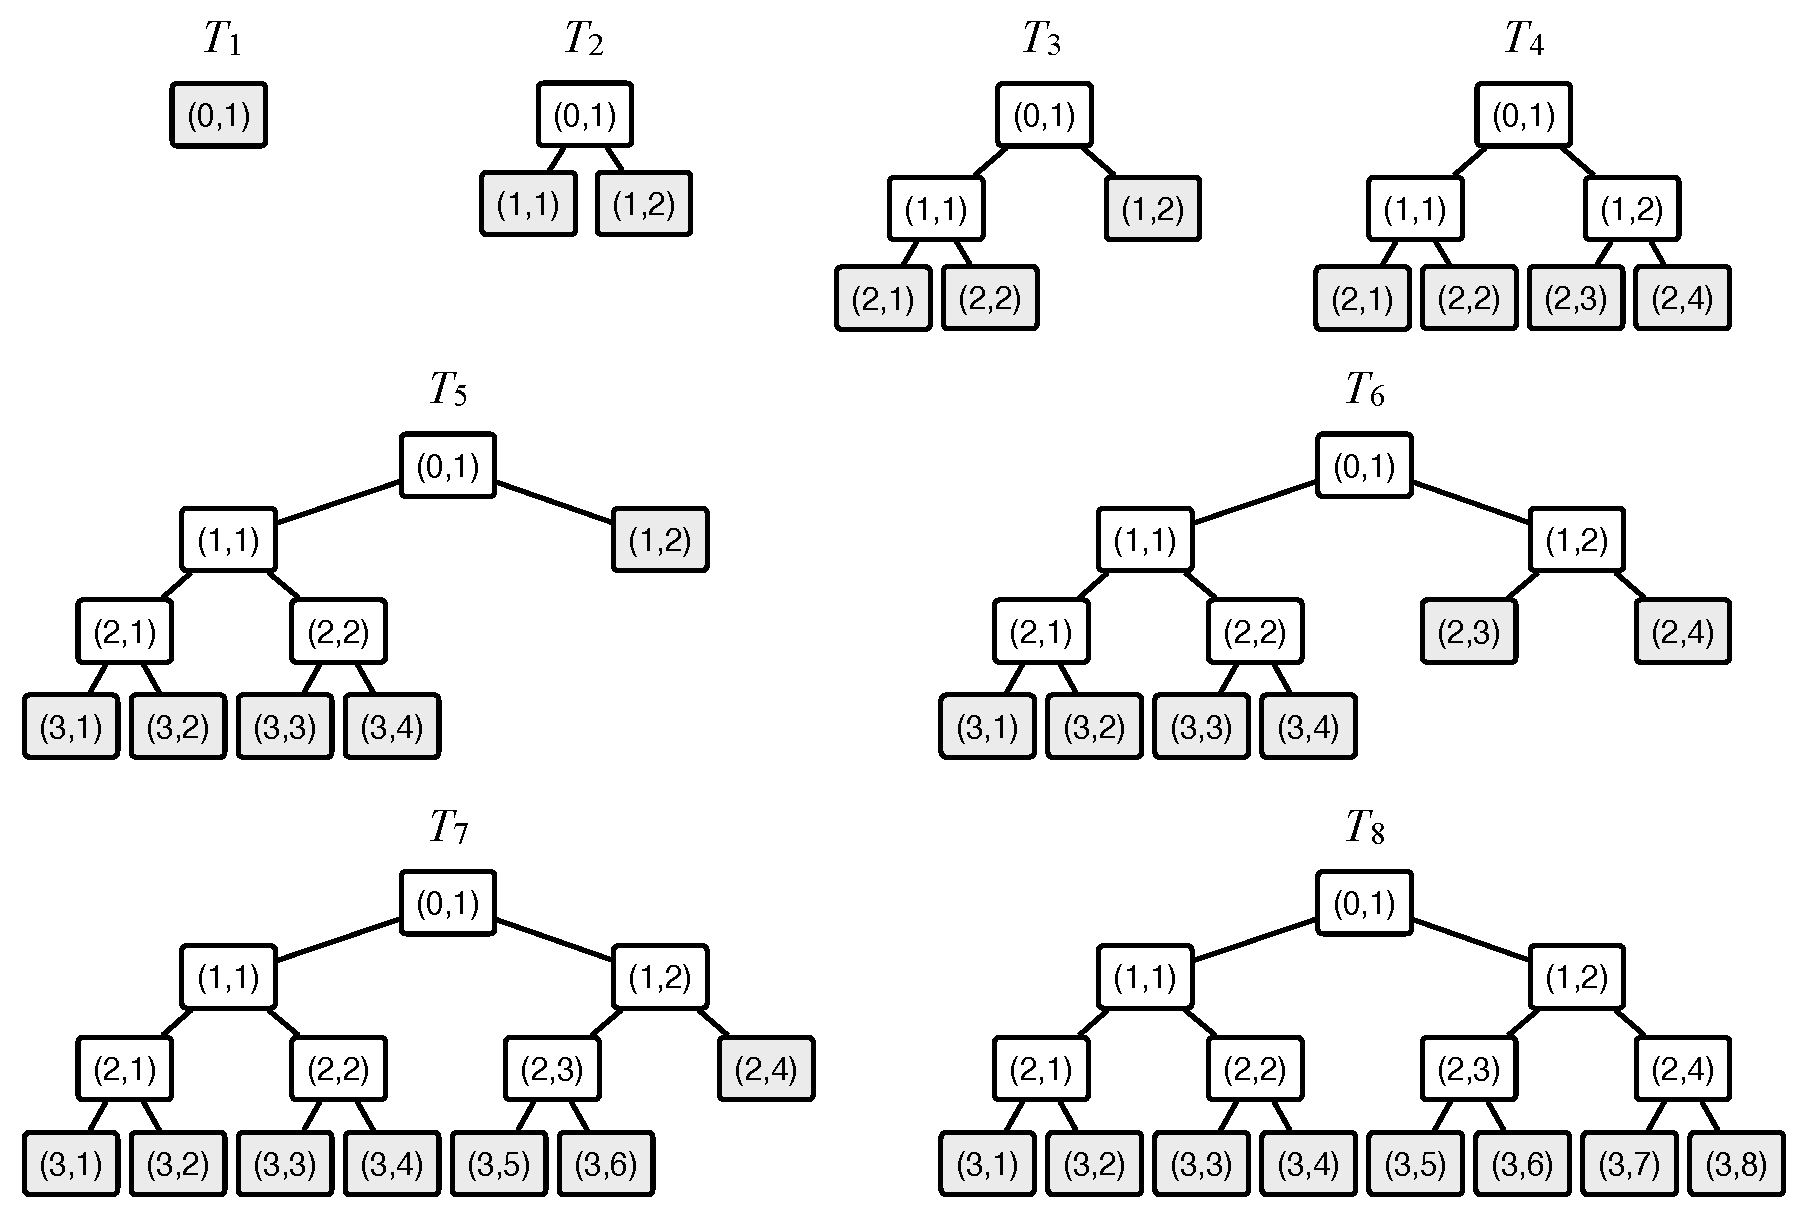
\includegraphics[width=0.8\textwidth]{\FigureFolder/mt-arbitrary-length}
\caption[Trees for message length $\MTMessageLength$ from $1$ to $8$.]{The trees $(\MTGraph_{\MTMessageLength})_{\MTMessageLength \in [8]}$ for messages lengths $\MTMessageLength \in [8]$ from \Cref{definition:binary-tree-arbitrary-number-of-leaves-alt-1}. The trees $\MTGraph_{1},\MTGraph_{2},\MTGraph_{4},\MTGraph_{8}$ coincide with the trees defined in \Cref{chapter:merkle-commitment} for messages whose length is a power of $2$ (see \Cref{definition:mt-graph}).}
\label{figure:mt-arbitrary-length}
\end{figure}

%%%%%%%%%%%%%%%%%%%%%%%%%%%%%%%%%%%%%%%%%%%%%%%%%%%%%%%%%%%%%%%%%%%%%%%%%%%%%%%
%%%%%%%%%%%%%%%%%%%%%%%%%%%%%%%%%%%%%%%%%%%%%%%%%%%%%%%%%%%%%%%%%%%%%%%%%%%%%%%
%%%%%%%%%%%%%%%%%%%%%%%%%%%%%%%%%%%%%%%%%%%%%%%%%%%%%%%%%%%%%%%%%%%%%%%%%%%%%%%
\section{Path pruning}
\label{section:compressing-opening-proof}

We discuss \textbf{path pruning}, a method to reduce the size of Merkle opening proofs that authenticate multiple locations of the committed message vector. For simplicity, we focus on the case of the Merkle commitment scheme discussed in \Cref{chapter:merkle-commitment}, which involves perfect binary trees that support message lengths that are powers of two. However, the method of path pruning straightforwardly extends to work for the generalized Merkle tree based on any tree discussed in \Cref{section:any-message-length}.

An authentication path for location $\MTMessageIndex$ has the following structure (\Cref{equation:mt-authpath-structure}):
\begin{equation*}
\MTAuthPath_{\MTMessageIndex}
\DefineEqual
\big(
\MTSaltString_{\MTMessageIndex}
,
(\MTVertexLabel_{\MTGraphVertex})_{\MTGraphVertex \in \MTCoPath(\MTMessageIndex)}
\big)
=
\big(
\MTSaltString_{\MTMessageIndex}
,
(\MTVertexLabelByCoPath{\MTMessageIndex}{\MTLayer})_{\MTLayer \in \{1,\dots,\MTDepth\}}
\big)
\end{equation*}
where $\MTSaltString_{\MTMessageIndex}$ is a salt string and $(\MTVertexLabel_{\MTGraphVertex})_{\MTGraphVertex \in \MTCoPath(\MTMessageIndex)}$ are the commitments associated to the $\MTDepth$ vertices in the copath of $\MTMessageIndex$. In particular, $\MTAuthPath_{\MTMessageIndex}$ has size $\MTSaltSize + \MTDepth\ROOutputSize$ because the salt string consists of $\MTSaltSize$ bits and each of the $\MTDepth$ commitments consists of $\ROOutputSize$ bits. All of this information is necessary to validate $\MTAuthPath_{\MTMessageIndex}$. Nevertheless, if $\Cardinality{\MTMessageIndexSet}>1$ an opening proof $\MTProof = (\MTAuthPath_{\MTMessageIndex})_{\MTMessageIndex \in \MTMessageIndexSet}$ contains redundant information \emph{across} authentication paths,\footnote{This redundancy causes the delicate technical details in the discussion leading up to the design of $\MTSimulator$ in \Cref{construction:mt-simulator}, which samples a simulated Merkle commitment and opening proof.} enabling a \DoQuote{path pruning} optimization that reduces the size of $\MTProof$.

In more detail, without any optimizations, the size of an opening proof $\MTProof = (\MTAuthPath_{\MTMessageIndex})_{\MTMessageIndex \in \MTMessageIndexSet}$ for a subset $\MTMessageIndexSet \subseteq [\MTMessageLength]$ is $\Cardinality{\MTMessageIndexSet} \cdot (\MTSaltSize + \MTDepth\ROOutputSize)$ because it consists of $\Cardinality{\MTMessageIndexSet}$ authentication paths each of size $\MTSaltSize + \MTDepth\ROOutputSize$. The salt strings $(\MTSaltString_{\MTMessageIndex})_{\MTMessageIndex \in \MTMessageIndexSet}$ that contribute a size of $\Cardinality{\MTMessageIndexSet} \cdot \MTSaltSize$ are necessary and cannot be removed. (Though if privacy is not a goal, then there are no salts as $\MTSaltSize=0$, so the term $\Cardinality{\MTMessageIndexSet} \cdot \MTSaltSize$ disappears.) If $\Cardinality{\MTMessageIndexSet}>1$ then not all $\Cardinality{\MTMessageIndexSet} \cdot \MTDepth\ROOutputSize$ bits contributed by $((\MTVertexLabel_{\MTGraphVertex})_{\MTGraphVertex \in \MTCoPath(\MTMessageIndex)})_{\MTMessageIndex \in \MTMessageIndexSet}$ are necessary. There are redundant commitments across multiple authentication paths that can be removed.

In \Cref{section:path-pruning-example}, we build intuition on the optimization via some examples. Then, in \Cref{section:path-pruning-general}, we discuss the general case of the optimization and the savings that it brings. Finally, in \Cref{section:path-pruning-security}, we discuss how the optimization impacts security properties.

%%%%%%%%%%%%%%%%%%%%%%%%%%%%%%%%%%%%%%%%%%%%%%%%%%%%%%%%%%%%%%%%%%%%%%%%%%%%%%%
%%%%%%%%%%%%%%%%%%%%%%%%%%%%%%%%%%%%%%%%%%%%%%%%%%%%%%%%%%%%%%%%%%%%%%%%%%%%%%%
\subsection[Examples for message length 8]{Examples for $\MTMessageLength=8$}
\label{section:path-pruning-example}

Consider the Merkle commitment scheme for message length $\MTMessageLength=8$. In this case the binary tree is $\MTGraph_{3}$, since $\MTDepth=\log_{2} 8=3$. We discuss how to eliminate redundancy among the commitments $((\MTVertexLabel_{\MTGraphVertex})_{\MTGraphVertex \in \MTCoPath(\MTMessageIndex)})_{\MTMessageIndex \in \MTMessageIndexSet}$ for three different examples of sets $\MTMessageIndexSet \subseteq [8]$.

\parhead{Duplicate commitments}
The same vertex may appear in multiple copaths, and thus the same commitment is included in each of the corresponding authentication paths. For example, in \Cref{figure:mt-prune-1} we consider the case of $\MTMessageIndexSet = \{5,6\}$. The corresponding co-paths are:
\begin{align*}
\MTCoPath(5) &= \big( (3,5),(2,4),(1,1) \big) \enspace, \\
\MTCoPath(6) &= \big( (3,6),(2,4),(1,1) \big) \enspace.
\end{align*}
We see that the vertices $(2,4)$ and $(1,1)$ appear in both copaths, which means that the commitments $\MTVertexLabelByName{2}{4}$ and $\MTVertexLabelByName{1}{1}$ are included in both authentication paths $\MTAuthPath_{5}$ and $\MTAuthPath_{6}$. Of course, we can omit duplicate copies of commitments in an opening proof. Overall, the opening proof $\MTProof$ only needs to include commitments for the following vertices (blue in \Cref{figure:mt-prune-2}):
\begin{equation*}
\big\{ (1,1),(2,4) \big\}
\enspace.
\end{equation*}

\parhead{Derivable commitments}
A commitment computed as part of the copath for an entry may be the result of an oracle query to check the copath of another entry. For example, in \Cref{figure:mt-prune-2} we consider the case of $\MTMessageIndexSet = \{3,6\}$. The corresponding copaths are:
\begin{align*}
\MTCoPath(3) &= \big( (3,4),(2,1),(1,2) \big) \enspace, \\
\MTCoPath(6) &= \big( (3,6),(2,4),(1,1) \big) \enspace.
\end{align*}
Here there are no duplicate vertices. Nevertheless, the computation to check $\MTAuthPath_{3}$ produces the commitment $\MTVertexLabelByName{1}{1}$ as an answer from the oracle, and therefore there is no need to include it in $\MTAuthPath_{6}$. Similarly, the computation to check $\MTAuthPath_{3}$ produces $\MTVertexLabelByName{1}{2}$ as an answer from the oracle, and therefore there is no need to include it in $\MTAuthPath_{3}$. Overall, the opening proof $\MTProof$ only needs to include commitments for the following vertices (blue in \Cref{figure:mt-prune-2}):
\begin{equation*}
\big\{ (3,4),(3,5),(2,1),(2,4) \big\}
\enspace.
\end{equation*}
In the extreme, suppose one considers the authentication paths for all leaves in a particular subtree. In that case, it suffices to provide the authentication path for the root vertex of that subtree, and the rest can be recovered by the checking algorithm by computing the commitments of the relevant inner vertices from the leaf commitments.

\parhead{Duplicate and derivable}
There could be both duplicate commitments and derivable commitments across multiple authentication paths. For example, in \Cref{figure:mt-prune-3} we consider the case of $\MTMessageIndexSet = \{1,3,5,6\}$. The corresponding copaths are:
\begin{align*}
\MTCoPath(1) &= \big( (3,2),(2,2),(1,2) \big) \enspace, \\
\MTCoPath(3) &= \big( (3,4),(2,1),(1,2) \big) \enspace, \\
\MTCoPath(5) &= \big( (3,5),(2,4),(1,1) \big) \enspace, \\
\MTCoPath(6) &= \big( (3,6),(2,4),(1,1) \big) \enspace.
\end{align*}
By removing duplicate commitments and derivable commitments, we see that the opening proof $\MTProof$ only needs to include commitments for the following vertices (blue in \Cref{figure:mt-prune-3}):
\begin{equation*}
\big\{ (3,2),(3,4),(2,4) \big\}
\enspace.
\end{equation*}

\begin{figure}[htp!]
\centering
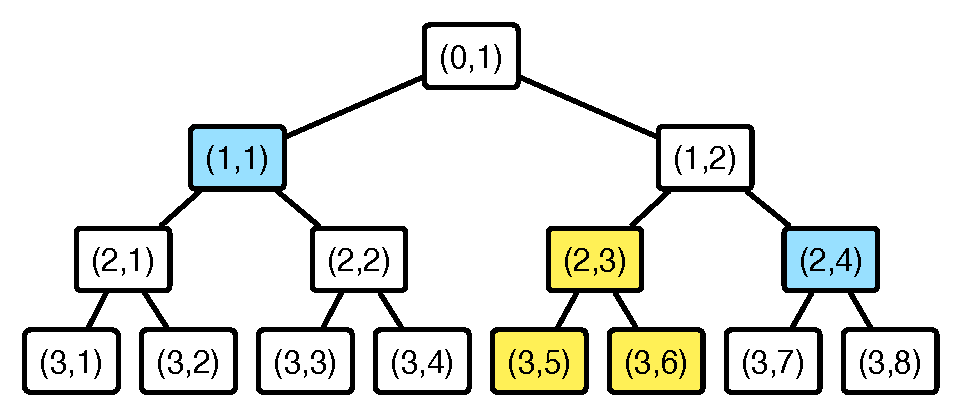
\includegraphics[width=0.5\textwidth]{\FigureFolder/mt-prune-1}
\caption[Authenticating $\MTMessageIndexSet = \{5,6\}$ in the tree $\MTGraph_{3}$.]{The binary tree $\MTGraph_{3}$ with the leaves corresponding to locations $\MTMessageIndexSet = \{5,6\}$ highlighted in yellow, and the minimal set of vertices to authenticate these locations highlighted in blue.}
\label{figure:mt-prune-1}
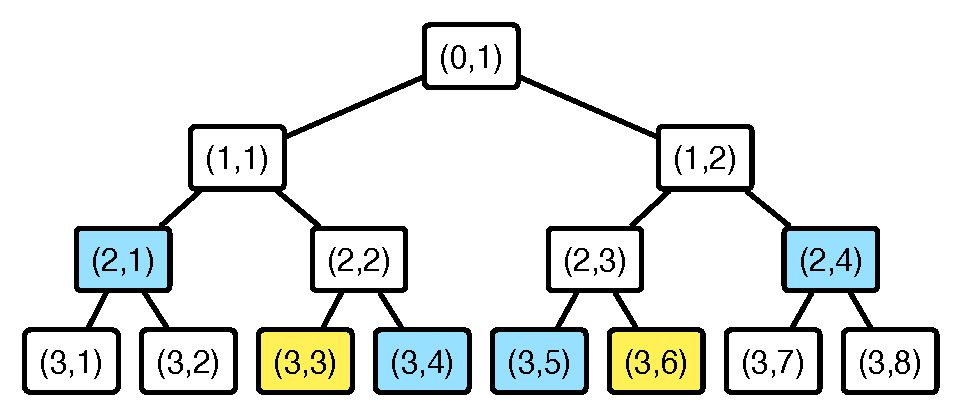
\includegraphics[width=0.5\textwidth]{\FigureFolder/mt-prune-2}
\caption[Authenticating $\MTMessageIndexSet = \{3,6\}$ in the tree $\MTGraph_{3}$.]{The binary tree $\MTGraph_{3}$ with the leaves corresponding to locations $\MTMessageIndexSet = \{3,6\}$ highlighted in yellow, and the minimal set of vertices to authenticate these locations highlighted in blue.}
\label{figure:mt-prune-2}
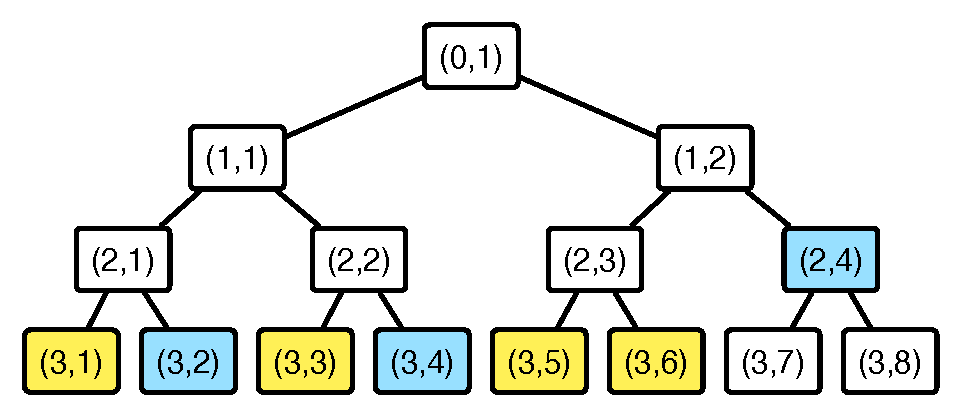
\includegraphics[width=0.5\textwidth]{\FigureFolder/mt-prune-3}
\caption[Authenticating $\MTMessageIndexSet = \{1,3,5,6\}$ in the tree $\MTGraph_{3}$.]{The binary tree $\MTGraph_{3}$ with the leaves corresponding to locations $\MTMessageIndexSet = \{1,3,5,6\}$ highlighted in yellow, and the minimal set of vertices to authenticate these locations highlighted in blue.}
\label{figure:mt-prune-3}
\end{figure}

%%%%%%%%%%%%%%%%%%%%%%%%%%%%%%%%%%%%%%%%%%%%%%%%%%%%%%%%%%%%%%%%%%%%%%%%%%%%%%%
%%%%%%%%%%%%%%%%%%%%%%%%%%%%%%%%%%%%%%%%%%%%%%%%%%%%%%%%%%%%%%%%%%%%%%%%%%%%%%%
\subsection{The general case}
\label{section:path-pruning-general}

The path pruning optimization is captured by a function $\MTDeriveVertexSet$ that maps an index set $\MTMessageIndexSet \subseteq [\MTMessageLength]$ to a vertex set $\MTCoPathVarVertexSet \subseteq \MTVertexSet_{\MTMessageLength}$ that is \emph{the minimal set of vertices for authenticating every index in $\MTMessageIndexSet$}. (Recall that $\MTVertexSet_{\MTMessageLength}$ is the vertex set of the perfect binary tree $\MTGraph_{\MTMessageLength}$ in \Cref{definition:mt-graph}.)

Informally, the computation of $\MTCoPathVarVertexSet$ from $\MTMessageIndexSet$ proceeds layer by layer, starting from the leaves. In the leaf layer, mark the vertices corresponding to the set $\MTMessageIndexSet$, and include in $\MTCoPathVarVertexSet$ any unmarked vertex whose sibling is marked; then mark the parent of any vertex that is marked. Then repeat this procedure for the next layer. Output the set $\MTCoPathVarVertexSet$ when this recursive procedure terminates.
\begin{itemize}[noitemsep]
  \item[] $\MTDeriveVertexSet(\MTMessageIndexSet)$:
\begin{enumerate}[nolistsep]
  \item Initialize $\MTPathVertexSet_{\MTDepth} \DefineEqual \{(\MTDepth,\MTMessageIndex)\}_{\MTMessageIndex \in \MTMessageIndexSet}$ and empty sets $\MTPathVertexSet_{\MTDepth-1},\dots,\MTPathVertexSet_{1},\MTPathVertexSet_{0}$.
  \item Initialize empty sets $\MTCoPathVarVertexSet_{\MTDepth},\dots,\MTCoPathVarVertexSet_{1}$.
  \item For $\MTLayer = \MTDepth-1,\dots,1,0$ (in this order) and for $\MTMessageIndex \in [2^{\MTLayer}]$:
  \begin{enumerate}[nolistsep]
    \item If $(\MTLayer+1,2\MTMessageIndex-1) \notin \MTPathVertexSet_{\MTLayer+1}$ and $(\MTLayer+1,2\MTMessageIndex) \notin \MTPathVertexSet_{\MTLayer+1}$ then do nothing.
    \item \label{step:path-pruning-general-on-path}
    If $(\MTLayer+1,2\MTMessageIndex-1) \in \MTPathVertexSet_{\MTLayer+1}$ or $(\MTLayer+1,2\MTMessageIndex) \in \MTPathVertexSet_{\MTLayer+1}$ then:
    \begin{itemize}[nolistsep]
      \item if $(\MTLayer+1,2\MTMessageIndex-1) \notin \MTPathVertexSet_{\MTLayer+1}$ then add $(\MTLayer+1,2\MTMessageIndex-1)$ to $\MTCoPathVarVertexSet_{\MTLayer+1}$;
      \item if $(\MTLayer+1,2\MTMessageIndex) \notin \MTPathVertexSet_{\MTLayer+1}$ then add $(\MTLayer+1,2\MTMessageIndex)$ to $\MTCoPathVarVertexSet_{\MTLayer+1}$;
      \item add $(\MTLayer,\MTMessageIndex)$ to $\MTPathVertexSet_{\MTLayer}$.
    \end{itemize}
  \end{enumerate}
  \item Output $\MTCoPathVarVertexSet \DefineEqual \cup_{\MTLayer \in [\MTDepth]} \MTCoPathVarVertexSet_{\MTLayer}$.
\end{enumerate}
\end{itemize}
The minimal set of vertices output by $\MTDeriveVertexSet(\MTMessageIndexSet)$ has an elegant characterization: the vertices in the copaths for $\MTMessageIndexSet$ but not the paths for $\MTMessageIndexSet$. In fact, not by chance, this set of vertices has appeared before in the context of the hiding property of Merkle commitment schemes in \Cref{lemma:mt-privacy}.

\begin{lemma}
\label{lemma:path-pruning-is-copaths-minus-paths}
$\MTDeriveVertexSet(\MTMessageIndexSet) = \MTCoPath(\MTMessageIndexSet) \setminus \MTPath(\MTMessageIndexSet)$.
\end{lemma}

\begin{proof}
The sets $\MTPathVertexSet_{\MTDepth},\dots,\MTPathVertexSet_{0}$ consist of the vertices in $\MTPath(\MTMessageIndexSet)$. Indeed, $\MTPathVertexSet_{\MTDepth}$ is initialized with the leaf vertices corresponding to the indices in $\MTMessageIndexSet$. Then, for $\MTLayer = \MTDepth-1,\dots,1,0$, the algorithm sets $\MTPathVertexSet_{\MTLayer}$ to equal the parents of the vertices in $\MTPathVertexSet_{\MTLayer+1}$. We conclude that $\idxcup{\MTLayer \in \{0,1,\dots,\MTDepth\}} \MTPathVertexSet_{\MTLayer} = \MTPath(\MTMessageIndexSet)$.

The output of the algorithm is $\MTCoPathVarVertexSet \DefineEqual \cup_{\MTLayer \in [\MTDepth]} \MTCoPathVarVertexSet_{\MTLayer}$. We argue that $\MTCoPathVarVertexSet = \MTCoPath(\MTMessageIndexSet) \setminus \MTPath(\MTMessageIndexSet)$.
\begin{itemize}[nolistsep]
  \item If a vertex is in $\idxcup{\MTLayer \in \{0,1,\dots,\MTDepth\}} \MTPathVertexSet_{\MTLayer} = \MTPath(\MTMessageIndexSet)$ then the algorithm does not add the vertex to $\MTCoPathVarVertexSet$.
  \item If the algorithm adds a vertex to $\MTCoPathVarVertexSet$ then the vertex is the sibling of a vertex in $\idxcup{\MTLayer \in \{0,1,\dots,\MTDepth\}} \MTPathVertexSet_{\MTLayer} = \MTPath(\MTMessageIndexSet)$, and hence the vertex is in $\MTCoPath(\MTMessageIndexSet)$.
  \item Fix $\MTGraphVertex \in \MTCoPath(\MTMessageIndexSet) \setminus \MTPath(\MTMessageIndexSet)$. If $\MTGraphVertex$ is an odd vertex we can write $\MTGraphVertex=(\MTLayer+1,2\MTMessageIndex-1)$ for $\MTLayer \in \{0,1,\dots,\MTDepth-1\}$ and $\MTMessageIndex \in [2^{\MTLayer}]$, or else if $\MTGraphVertex$ is an even vertex we can write $\MTGraphVertex=(\MTLayer+1,2\MTMessageIndex)$. Suppose without loss of generality that $\MTGraphVertex$ is odd (the even case is similar). The sibling $\MTGraphVertex'=(\MTLayer+1,2\MTMessageIndex)$ of $\MTGraphVertex$ is in $\MTPathVertexSet_{\MTLayer+1} \subseteq \MTPath(\MTMessageIndexSet)$, so in the $(\MTLayer,\MTMessageIndex)$-th iteration of the algorithm the condition in \Cref{step:path-pruning-general-on-path} holds. Since $\MTGraphVertex \not\in \MTPath(\MTMessageIndexSet)$, we know that $\MTGraphVertex \not\in \MTPathVertexSet_{\MTLayer+1}$. Hence the algorithm adds $\MTGraphVertex$ to $\MTCoPathVarVertexSet_{\MTLayer+1} \subseteq \MTCoPathVarVertexSet$.
\end{itemize}
\end{proof}

Path pruning requires modifying the algorithms $\MTOpen$ and $\MTCheck$ of the Merkle commitment scheme in \Cref{section:merkle-commitment-definition} to the constructions $\MTOpen_{\star}$ and $\MTCheck_{\star}$ below.
\begin{itemize}

  \item $\MTOpen_{\star}^{\ROFunction}(\MTTrapdoor, \MTMessageIndexSet) \to \MTProof$
\begin{enumerate}[nolistsep]
  \item Compute the set of vertices $\MTCoPathVarVertexSet \DefineEqual \MTDeriveVertexSet(\MTMessageIndexSet)$.
  \item Output the opening proof
\begin{equation}
\label{equation:mt-compressed-opening-proof}
\MTProof \DefineEqual
\Big(
(\MTSaltString_{\MTMessageIndex})_{\MTMessageIndex \in \MTMessageIndexSet},
(\MTVertexLabelByName{\MTLayer}{\MTMessageIndex})_{(\MTLayer,\MTMessageIndex) \in \MTDeriveVertexSet(\MTMessageIndexSet)}
\Big)
\enspace.
\end{equation}
\end{enumerate}
Namely, the opening proof $\MTProof$ includes the salts for all the authenticated leaves and the commitments for vertices in the set $\MTDeriveVertexSet(\MTMessageIndexSet)$. The size of the opening proof $\MTProof$ is
\begin{equation}
\label{equation:mt-compressed-size-expression}
\Cardinality{\MTMessageIndexSet} \cdot \MTSaltSize
+
\Cardinality{\MTDeriveVertexSet(\MTMessageIndexSet)} \cdot \ROOutputSize
\enspace.
\end{equation}
If privacy is not desired then $\MTSaltSize=0$, in which case the size of $\MTProof$ is $\Cardinality{\MTDeriveVertexSet(\MTMessageIndexSet)} \cdot \ROOutputSize$.

  \item $\MTCheck_{\star}^{\ROFunction}(\MTCommitment,\MTMessageIndexSet,\MTMessageSubVector,\MTProof) \to b$
  \begin{enumerate}[nolistsep]
    \item Parse $\MTProof$ as in \Cref{equation:mt-compressed-opening-proof}.
    \item For every $\MTMessageIndex \in \MTMessageIndexSet$, compute the commitment $\MTVertexLabelByName{\MTDepth}{\MTMessageIndex} \DefineEqual \ROFunction(\MTMessageSubVector[\MTMessageIndex],\MTSaltString_{\MTMessageIndex})$.
    \item For $\MTLayer = \MTDepth-1,\dots,0$ (in this order) and $\MTMessageIndex \in [2^{\MTLayer}]$: \\ \phantom{aa} if $(\MTLayer,\MTMessageIndex) \in \MTPath(\MTMessageIndexSet)$ then set $\MTVertexLabelByName{\MTLayer}{\MTMessageIndex} \DefineEqual \ROFunction(\MTVertexLabelByName{\MTLayer+1}{2\MTMessageIndex-1},\MTVertexLabelByName{\MTLayer+1}{2\MTMessageIndex}) \in \Bits^{\ROOutputSize}$.
    \item Check that $\MTCommitment = \MTVertexLabelByName{0}{1}$. (Note that $(0,1) \in \MTPath(\MTMessageIndexSet)$.)
  \end{enumerate}

The algorithm $\MTCheck_{\star}$ makes $\Cardinality{\MTPath(\MTMessageIndexSet)}$ queries to the random oracle, and runs in time proportional to $\Cardinality{\MTCoPath(\MTMessageIndexSet) \cup \MTPath(\MTMessageIndexSet)}$.

\end{itemize}

\parhead{Efficiency of path pruning}
The size of an opening proof $\MTProof$ with path pruning is $\Cardinality{\MTMessageIndexSet} \cdot \MTSaltSize + \Cardinality{\MTDeriveVertexSet(\MTMessageIndexSet)} \cdot \ROOutputSize$ (see \Cref{equation:mt-compressed-size-expression}), compared to $\Cardinality{\MTMessageIndexSet} \cdot \MTSaltSize + \Cardinality{\MTMessageIndexSet} \cdot \MTDepth \cdot \ROOutputSize$ without path pruning. Therefore the effectiveness of path pruning is determined by the size of the set $\MTDeriveVertexSet(\MTMessageIndexSet)$.

It is clear that $\Cardinality{\MTDeriveVertexSet(\MTMessageIndexSet)} \leq \Cardinality{\MTMessageIndexSet} \cdot \MTDepth$. But how does $\Cardinality{\MTDeriveVertexSet(\MTMessageIndexSet)}$ behave?

Intuitively, as the size of $\MTMessageIndexSet$ increases so does the size of $\MTDeriveVertexSet(\MTMessageIndexSet)$. However when $\Cardinality{\MTMessageIndexSet} = [\MTMessageLength]$ (all locations) then $\MTDeriveVertexSet(\MTMessageIndexSet)=\emptyset$ because there is no need to provide any commitments to recover the Merkle commitment $\MTCommitment$ starting all message entries and salt strings. Hence, as $\MTMessageIndexSet$ increases in size, the size of $\MTDeriveVertexSet(\MTMessageIndexSet)$ eventually decreases and becomes zero.

In order to build intuition it is useful to discuss two extreme settings.
\begin{itemize}
  \item \emph{Good case.}
  The good case is when the locations in $\MTMessageIndexSet$ are all the leaves of a subtree of $\MTGraph_{\MTMessageLength}$ (in which case $\Cardinality{\MTMessageIndexSet}$ is a power of $2$). In this case, the commitment corresponding to the root vertex of the subtree can be deduced from the message entries and salt strings over $\MTMessageIndexSet$, without the need for any additional information. From thereon it suffices to provide commitments for vertices in the copath of the root vertex, and this copath consists of $\MTDepth-\log_{2}\Cardinality{\MTMessageIndexSet}$ vertices. Overall in this case $\Cardinality{\MTDeriveVertexSet(\MTMessageIndexSet)}=\MTDepth-\log_{2}\Cardinality{\MTMessageIndexSet}$.

\Cref{figure:mt-prune-good-case} illustrates this phenomenon for message length $\MTMessageLength=16$ and index set $\MTMessageIndexSet = \{1,2,3,4\}$, in which case the tree depth is $\MTDepth=4$. The yellow leaf vertices are the opened locations and the blue vertices are those whose commitments are included in the opening proof. We see that the size of $\MTDeriveVertexSet(\MTMessageIndexSet)$ is $2$, which agrees with the expression $\MTDepth-\log_{2}\Cardinality{\MTMessageIndexSet} = 4 - \log_{2} 4 = 4-2 = 2$.

  \item \emph{Bad case.}
  The bad case is when the locations in $\MTMessageIndexSet$ are as spread out as possible, for example take the set $\MTMessageIndexSet = \{j \cdot \frac{\MTMessageLength}{\Cardinality{\MTMessageIndexSet}} \}_{j \in \Cardinality{\MTMessageIndexSet}}$ (and assume that $\Cardinality{\MTMessageIndexSet}$ divides $\MTMessageLength$, in which case $\Cardinality{\MTMessageIndexSet}$ is a power of $2$). In this case each location is \DoQuote{alone} in a subtree of $\frac{\MTMessageLength}{\Cardinality{\MTMessageIndexSet}}$ leaves; for each of these $\Cardinality{\MTMessageIndexSet}$ subtrees, computing the commitment of the root vertex requires obtaining commitments corresponding to a copath of length $\log_{2} \frac{\MTMessageLength}{\Cardinality{\MTMessageIndexSet}} = \log_{2} \MTMessageLength - \log_{2} \Cardinality{\MTMessageIndexSet} = \MTDepth-\log_{2}\Cardinality{\MTMessageIndexSet}$. Thereon, given the commitments of the root vertices of the $\Cardinality{\MTMessageIndexSet}$ subtrees, one can compute the commitment of the root vertex of $\MTGraph_{\MTMessageLength}$ without any additional information. Overall in this case $\Cardinality{\MTDeriveVertexSet(\MTMessageIndexSet)}= \Cardinality{\MTMessageIndexSet} \cdot (\MTDepth-\log_{2}\Cardinality{\MTMessageIndexSet})$.

\Cref{figure:mt-prune-bad-case} illustrates this phenomenon for message length $\MTMessageLength=16$ and index set $\MTMessageIndexSet = \{2,7,12,14\}$, in which case the tree depth is $\MTDepth=4$. The yellow leaf vertices are the opened locations and the blue vertices are those whose commitments are included in the opening proof. We see that the size of $\MTDeriveVertexSet(\MTMessageIndexSet)$ is $8$, which agrees with the expression $\Cardinality{\MTMessageIndexSet} \cdot (\MTDepth-\log_{2}\Cardinality{\MTMessageIndexSet}) = 4 \cdot (4 - \log_{2} 4) = 8$.

\end{itemize}
The above examples represent extremal situations, as captured by the following lemma. The upper bound in the lemma improves on the prior (trivial) upper bound $\Cardinality{\MTMessageIndexSet} \cdot \MTDepth$.

\begin{lemma}
\label{lemma:path-pruning-lower-and-upper}
$\MTDepth-\log_{2}\Cardinality{\MTMessageIndexSet}
\leq
\Cardinality{\MTDeriveVertexSet(\MTMessageIndexSet)}
\leq
\Cardinality{\MTMessageIndexSet} \cdot (\MTDepth-\log_{2}\Cardinality{\MTMessageIndexSet})
$.
\end{lemma}

\begin{proof}
We establish the lower bound and the upper bound separately.

\parhead{Lower bound}
First we assume that $\Cardinality{\MTMessageIndexSet}$ is a power of 2, and then show how to handle the general case. The case where $\Cardinality{\MTMessageIndexSet}$ is a power of $2$ follows from the claim below, where we set $k \DefineEqual \log_{2} \Cardinality{\MTMessageIndexSet}$.

\begin{claim}
\label{claim:lower-bound-mt-opening-size}
There exists a sequence of subsets $\MTMessageIndexSet_{0},\ldots,\MTMessageIndexSet_{k} \subseteq [\MTMessageLength]$ that satisfies the following.
\begin{enumerate}[nosep]
  \item $\MTMessageIndexSet_{0} = \MTMessageIndexSet$ and $\Cardinality{\MTMessageIndexSet_{0}} = \cdots = \Cardinality{\MTMessageIndexSet_{k}}$.
  \item For every $\MTLayer \in \{0,1,\dots,k-1\}$, $\Cardinality{\MTDeriveVertexSet(\MTMessageIndexSet_{\MTLayer+1})} \leq \Cardinality{\MTDeriveVertexSet(\MTMessageIndexSet_{\MTLayer})}$.
  \item $\Cardinality{\MTDeriveVertexSet(\MTMessageIndexSet_{k})} = \MTDepth-\log_{2}\Cardinality{\MTMessageIndexSet}$.
  \item For every $\MTLayer \in \{0,1,\ldots,k\}$ and every subtree of $\MTGraph_{\MTMessageLength}$ with $2^{\MTLayer}$ leaf vertices, either no leaf vertex of the subtree is in $\MTMessageIndexSet_{\MTLayer}$ or all of the leaf vertices of the subtree are in $\MTMessageIndexSet_{\MTLayer}$.
\end{enumerate}
\end{claim}

The claim suffices because
\begin{align*}
\MTDepth-\log_{2}\Cardinality{\MTMessageIndexSet}
=
\Cardinality{\MTDeriveVertexSet(\MTMessageIndexSet_{k})}
\leq
\Cardinality{\MTDeriveVertexSet(\MTMessageIndexSet_{0})}
=
\Cardinality{\MTDeriveVertexSet(\MTMessageIndexSet)}
\enspace.
\end{align*}

\begin{proof}[Proof of \Cref{claim:lower-bound-mt-opening-size}]
We define $\MTMessageIndexSet_{0} \DefineEqual \MTMessageIndexSet$ and then recursively define the other subsets.

Given $\MTMessageIndexSet_{\MTLayer}$ that satisfies the above properties (for index $\MTLayer$), we initially set $\MTMessageIndexSet_{\MTLayer+1} \DefineEqual \MTMessageIndexSet_{\MTLayer}$ and then modify $\MTMessageIndexSet_{\MTLayer+1}$ so that it satisfies the above properties (for index $\MTLayer+1$).

Suppose that there exists a subtree $\MTGraph$ of size $2^{\MTLayer+1}$ whose leaf vertices partially overlap with $\MTMessageIndexSet_{\MTLayer+1}$. (If no such subtree $\MTGraph$ exists, then we are done since $\MTMessageIndexSet_{\MTLayer+1}$ satisfies all the required properties.) Let $\MTGraph_{L}$ be its left subtree and $\MTGraph_{R}$ be its right subtree. Either no leaf vertex of $\MTGraph_{L}$ is in $\MTMessageIndexSet_{\MTLayer+1}$ and all leaf vertices of $\MTGraph_{R}$ are in $\MTMessageIndexSet_{\MTLayer+1}$, or vice versa (otherwise there would be a subtree of size $2^{\MTLayer}$ whose leaf vertices partially overlap with $\MTMessageIndexSet_{\MTLayer}$). Moreover, if one such subtree $\MTGraph$ exists, then another such subtree $\MTGraph'$ also exists (as $\Cardinality{\MTMessageIndexSet}$ is a power of $2$). Overall, there are subtrees $\MTGraph$ and $\MTGraph'$, with left and right subtrees for $\MTGraph_{L},\MTGraph_{R}$ (for $\MTGraph$) and $\MTGraph'_{L},\MTGraph'_{R}$ (for $\MTGraph'$). Moreover, assume (without loss of generality) that all leaf vertices of $\MTGraph_{L}$ and $\MTGraph'_{L}$ are in $\MTMessageIndexSet_{\MTLayer+1}$ and no leaf vertices of either $\MTGraph_{R}$ or $\MTGraph'_{R}$ are in $\MTMessageIndexSet_{\MTLayer+1}$.

We remove the leaf vertices of $\MTGraph'_{L}$ from $\MTMessageIndexSet_{\MTLayer+1}$ and add to $\MTMessageIndexSet_{\MTLayer+1}$ the leaf vertices of $\MTGraph_{R}$. This ensures that no leaf vertex of $\MTGraph'$ is in $\MTMessageIndexSet_{\MTLayer+1}$, and all leaf vertices of $\MTGraph$ are in $\MTMessageIndexSet_{\MTLayer+1}$. Moreover, this swap does not increase the size of $\MTDeriveVertexSet(\MTMessageIndexSet_{\MTLayer+1})$. The root vertex of $\MTGraph_{R}$ is in $\MTDeriveVertexSet(\MTMessageIndexSet_{\MTLayer})$ (in order to authenticate the leaf vertices of $\MTGraph_{L}$). After adding the leaf vertices of $\MTGraph_{R}$ to $\MTMessageIndexSet_{\MTLayer+1}$, this root vertex can be derived from the leaf vertices of $\MTGraph_{R}$, so it is not in $\MTDeriveVertexSet(\MTMessageIndexSet_{\MTLayer+1})$. Since the leaves of $\MTGraph'_{R}$ were removed from $\MTMessageIndexSet_{\MTLayer+1}$, commitments of other vertices might be added to $\MTDeriveVertexSet(\MTMessageIndexSet_{\MTLayer+1})$. The only vertex that might be added is the root vertex of $\MTGraph'_{R}$. Overall, one vertex has been removed and (at most) one is added, so $\Cardinality{\MTDeriveVertexSet(\MTMessageIndexSet_{\MTLayer+1})} \leq \Cardinality{\MTDeriveVertexSet(\MTMessageIndexSet_{\MTLayer})}$ (the size did not increase).

We continue this process until no such subtrees exist. At the end, $\MTMessageIndexSet_{\MTLayer+1}$ satisfies all properties.

Finally, since $2^{k}=\Cardinality{\MTMessageIndexSet}=\Cardinality{\MTMessageIndexSet_{k}}$, $\MTMessageIndexSet_{k}$ consists of all the leaf vertices of a subtree with $2^{k}$ leaf vertices, so, as discussed in the \DoQuote{good case} above the lemma, $\Cardinality{\MTDeriveVertexSet(\MTMessageIndexSet_{k})} = \MTDepth-\log_{2}\Cardinality{\MTMessageIndexSet_{k}} = \MTDepth-\log_{2}\Cardinality{\MTMessageIndexSet}$.
\end{proof}

If $\Cardinality{\MTMessageIndexSet}$ is not a power of $2$, then we define a subset $\MTMessageIndexSet' \subseteq \MTMessageIndexSet$ whose cardinality is a power of $2$ such that $\Cardinality{\MTDeriveVertexSet(\MTMessageIndexSet)} \geq \Cardinality{\MTDeriveVertexSet(\MTMessageIndexSet')}$. We derive $\MTMessageIndexSet'$ from $\MTMessageIndexSet$ by removing indices as follows. Initially set $\MTMessageIndexSet' \DefineEqual \MTMessageIndexSet$. If $2$ does not divide $\Cardinality{\MTMessageIndexSet'}$, there exists a leaf vertex in $\MTMessageIndexSet'$ whose sibling is not in $\MTMessageIndexSet'$; we remove this leaf vertex, which does not increase the size of $\MTDeriveVertexSet(\MTMessageIndexSet')$. Next, if $4$ does not divide $\Cardinality{\MTMessageIndexSet'}$, there exists a pair of sibling leaf vertices in $\MTMessageIndexSet'$ for which the children of their parent's sibling both are not in $\MTMessageIndexSet'$; we remove this pair of siblings (which are leaf vertices), which does not increase the size of $\MTDeriveVertexSet(\MTMessageIndexSet')$. This continues until $\Cardinality{\MTMessageIndexSet'}$ is a power of $2$.

At the end of this process, we obtain $\MTMessageIndexSet'$ for which we can apply the proved lower bound:
\begin{align*}
\Cardinality{\MTDeriveVertexSet(\MTMessageIndexSet)}
\geq \Cardinality{\MTDeriveVertexSet(\MTMessageIndexSet')}
\geq \MTDepth-\log_{2}\Cardinality{\MTMessageIndexSet'}
\geq \MTDepth-\log_{2}\Cardinality{\MTMessageIndexSet}
\enspace.
\end{align*}

\parhead{Upper bound}
First we assume that $\Cardinality{\MTMessageIndexSet}$ is a power of 2, and then we discuss the general case.

Again setting $k \DefineEqual \log_{2} \Cardinality{\MTMessageIndexSet}$, we perform a sequence of swaps on $\MTMessageIndexSet$ that do not decrease the size of $\MTDeriveVertexSet(\MTMessageIndexSet)$. Suppose that there exists a subtree $\MTGraph$ with $2^{\MTDepth - k}$ leaf vertices with at least two leaf vertices in $\MTMessageIndexSet$, denoted $\MTGraphVertex_{1},\MTGraphVertex_{2}$. Then, there exists a subtree $\MTGraph'$ of the same size with no leaf vertex in $\MTMessageIndexSet$ (as otherwise the total number of elements in $\MTMessageIndexSet$ would be larger than $2^{k} = \Cardinality{\MTMessageIndexSet})$. We remove from $\MTMessageIndexSet$ the index for $\MTGraphVertex_{2}$ and add to $\MTMessageIndexSet$ the index for an arbitrary leaf vertiex $\MTGraphVertex$ of $\MTGraph'$. Since $\MTGraph'$ had no leaf vertices in $\MTMessageIndexSet$, $\MTDeriveVertexSet(\MTMessageIndexSet)$ now contains $\MTDepth - k$ new vertices for the copath of $\MTGraphVertex$. We removed $\MTGraphVertex_{2}$, and thus vertices from $\MTDeriveVertexSet(\MTMessageIndexSet)$ might be removed. However, since $\MTGraphVertex_{1},\MTGraphVertex_{2}$ are both in $\MTGraph$, at most $\MTDepth - k$ vertices are removed. Overall, the size of $\MTDeriveVertexSet(\MTMessageIndexSet)$ did not decrease.

We continue in this manner until all subtrees $\MTGraph$ with $2^{\MTDepth - k}$ leaves have exactly one leaf in $\MTMessageIndexSet$. At this point, the size of $\MTDeriveVertexSet(\MTMessageIndexSet)$ is upper bounded by $\Cardinality{\MTMessageIndexSet} \cdot (\MTDepth-\log_{2}\Cardinality{\MTMessageIndexSet})$ as discussed in the \DoQuote{bad case} above the lemma.

If $\Cardinality{\MTMessageIndexSet}$ is not a power of 2, then let $K$ be the smallest power of two with $K \geq \Cardinality{\MTMessageIndexSet}$. As explained in the \DoQuote{bad case} above, each location of $\MTMessageIndexSet$ is \DoQuote{alone} in a subtree of $\frac{\MTMessageLength}{K}$ leaves. Thus, each copath has size $\MTDepth-\log_{2} K$, and subtrees that do not have a leaf in $\MTMessageIndexSet$ (there are $K-\Cardinality{\MTMessageIndexSet}$ such subtrees) cause their root vertex to be in $\MTDeriveVertexSet(\MTMessageIndexSet)$. Overall, we get the bound
\begin{align*}
\Cardinality{\MTDeriveVertexSet(\MTMessageIndexSet)}
= & \Cardinality{\MTMessageIndexSet} \cdot (\MTDepth-\log_{2} K) + (K - \Cardinality{\MTMessageIndexSet})
\\ = &
\Cardinality{\MTMessageIndexSet} \cdot \left(\MTDepth - \log_{2}\Cardinality{\MTMessageIndexSet} - \log_{2} \frac{K}{\Cardinality{\MTMessageIndexSet}}\right) + (K-\Cardinality{\MTMessageIndexSet})
\\ = &
\Cardinality{\MTMessageIndexSet} \cdot (\MTDepth-\log_{2}\Cardinality{\MTMessageIndexSet}) - \Cardinality{\MTMessageIndexSet} \cdot \left( \log_{2} \frac{K}{\Cardinality{\MTMessageIndexSet}} - \frac{K}{\Cardinality{\MTMessageIndexSet}}+1\right)
\\ \geq &
\Cardinality{\MTMessageIndexSet} \cdot (\MTDepth-\log_{2}\Cardinality{\MTMessageIndexSet}) - \Cardinality{\MTMessageIndexSet} \cdot 0
\\ = &
\Cardinality{\MTMessageIndexSet} \cdot (\MTDepth-\log_{2}\Cardinality{\MTMessageIndexSet})
\enspace.
\end{align*}
Above, the inequality holds since the function $\log_{2}(x) - x + 1$ is non-negative for $x \in (1,2)$.
\end{proof}

The upper bound $\Cardinality{\MTMessageIndexSet} \cdot (\MTDepth-\log_{2}\Cardinality{\MTMessageIndexSet})$ is a concave function of $\MTMessageIndexSetSize \DefineEqual \Cardinality{\MTMessageIndexSet}$ over the interval $\{0,1,\dots,\MTMessageLength\}$: it equals $0$ when $\MTMessageIndexSetSize=0$ or $\MTMessageIndexSetSize=\MTMessageLength=2^{\MTDepth}$ (the two endpoints of the interval); and in between the function increases as $\MTMessageIndexSetSize$ increases up to some threshold $\MTMessageIndexSetSize_{0}$ and after that decreases. The threshold is where the derivative $\MTDepth-\log_{2}e - \log_{2}\MTMessageIndexSetSize$ of $\MTMessageIndexSetSize \cdot (\MTDepth-\log_{2}\MTMessageIndexSetSize)$ vanishes. Hence the (non-integer) threshold is $\MTMessageIndexSetSize_{0} \DefineEqual \frac{2^{\MTDepth}}{e} = \frac{\MTMessageLength}{e}$. Since $e \approx 2.72$, we know that $\MTMessageIndexSetSize_{0} \in [2^{\MTDepth-2},2^{\MTDepth-1}]$. This computation provides an indication for the location of the threshold for $\Cardinality{\MTDeriveVertexSet(\MTMessageIndexSet)}$, provided $\MTMessageIndexSet$ is sufficiently spread out (in which case $\Cardinality{\MTDeriveVertexSet(\MTMessageIndexSet)}$ is close to its upper bound $\Cardinality{\MTMessageIndexSet} \cdot (\MTDepth-\log_{2}\Cardinality{\MTMessageIndexSet})$).



\begin{figure}[htp!]
\centering
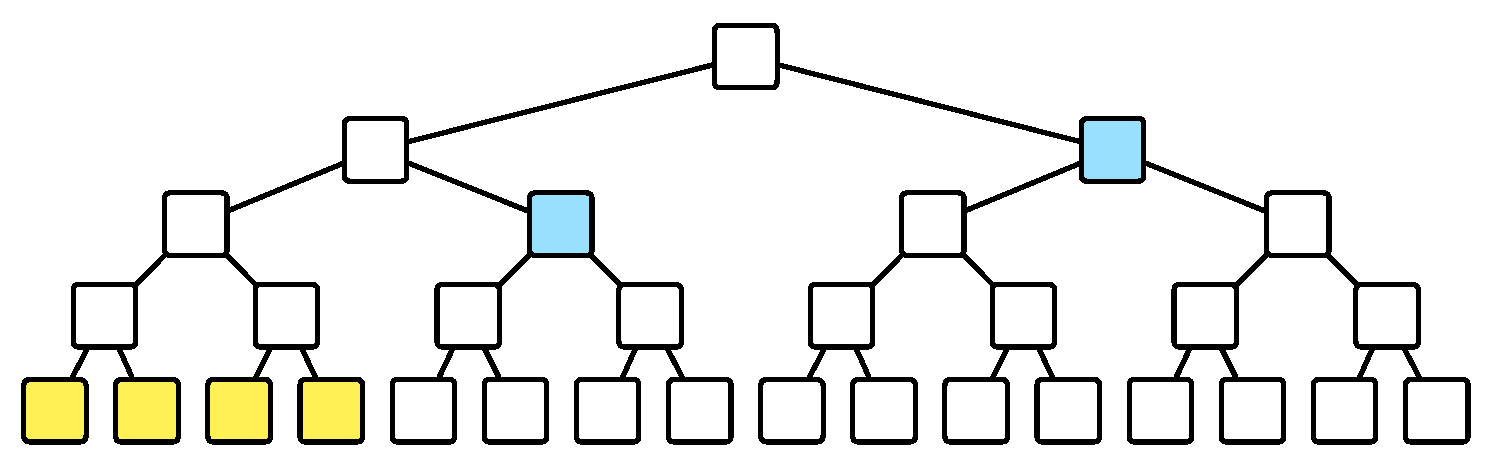
\includegraphics[width=0.5\textwidth]{\FigureFolder/mt-prune-good-case}
\caption[Example of path pruning for $\MTMessageLength=16$ and $\MTMessageIndexSet = \{1,2,3,4\}$.]{Example of path pruning for message length $\MTMessageLength=16$ and index set $\MTMessageIndexSet = \{1,2,3,4\}$.}
\label{figure:mt-prune-good-case}
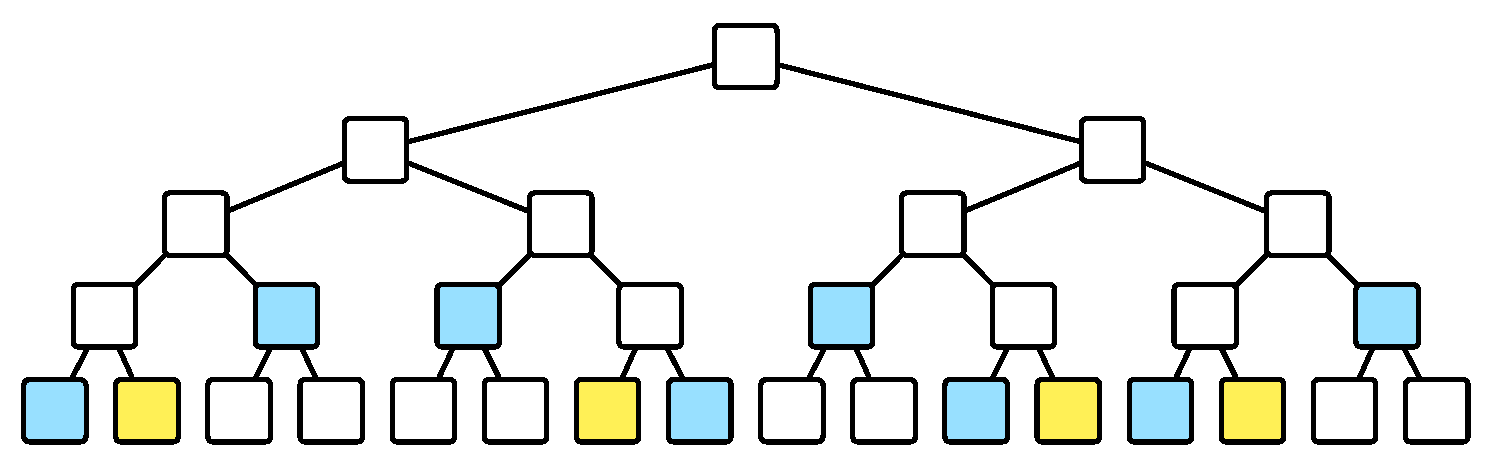
\includegraphics[width=0.5\textwidth]{\FigureFolder/mt-prune-bad-case}
\caption[Example of path pruning for $\MTMessageLength=16$ and $\MTMessageIndexSet = \{2,7,12,14\}$.]{Example of path pruning for message length $\MTMessageLength=16$ and index set $\MTMessageIndexSet = \{2,7,12,14\}$.}
\label{figure:mt-prune-bad-case}
\end{figure}


\parhead{Concrete efficiency}
In typical scenarios the set $\MTMessageIndexSet$ is the result of sampling locations from some high-entropy distribution, and so $\MTMessageIndexSet$ is likely to be reasonably spread out. In these cases we expect $\Cardinality{\MTDeriveVertexSet(\MTMessageIndexSet)}$ to be closer to the upper bound $\Cardinality{\MTMessageIndexSet} \cdot (\MTDepth-\log_{2}\Cardinality{\MTMessageIndexSet})$ rather than the lower bound $\MTDepth-\log_{2}\Cardinality{\MTMessageIndexSet}$. We illustrate this phenomenon via some empirical data.

We perform the following experiment. Consider the Merkle commitment scheme applied to a message of length $\MTMessageLength=2^{20}$. The message alphabet $\MTAlphabet$ does not affect the size of an opening proof, so we ignore it. We fix representative parameters: the output size of the random oracle is $\ROOutputSize=256$, and the salt size is $\MTSaltSize=128$. We consider a random subset $\MTMessageIndexSet$ of $[\MTMessageLength]=[2^{20}]$ of size $\MTMessageIndexSetSize$ for progressively larger values: we consider $\MTMessageIndexSetSize \in \{2^{i}\}_{i \in \{0,1,\dots,20\}}$. Note that $\MTMessageIndexSetSize=2^{0}=1$ corresponds to the case where one entry of the message is opened, and $\MTMessageIndexSetSize=2^{20}$ corresponds to the case where all entries of the message are opened. For each value of $\MTMessageIndexSetSize$ we collect several metrics.
\begin{itemize}
  \item
  Salts contribute $\MTMetric_{0} \DefineEqual \Cardinality{\MTMessageIndexSet} \cdot \MTSaltSize = \MTMessageIndexSetSize \cdot \MTSaltSize$ bits to the opening proof. These bits must be included in an opening proof (with or without path pruning).
  \item
  Without the path-pruning optimization, an opening proof includes a list of authentication paths that contribute $\MTMetric_{1} \DefineEqual \Cardinality{\MTMessageIndexSet} \cdot \MTDepth \cdot \ROOutputSize = \MTMessageIndexSetSize \cdot \MTDepth \cdot \ROOutputSize$ bits.
  \item
  With the path-pruning optimization, an opening proof includes (instead of the authentication paths) a list of commitments that contribute $\MTMetric_{2} \DefineEqual \Cardinality{\MTDeriveVertexSet(\MTMessageIndexSet)} \cdot \ROOutputSize$ bits. Note that $\MTMetric_{2}$ is a random variable that depends on the specific (random) choice of set $\MTMessageIndexSet$, because $\Cardinality{\MTDeriveVertexSet(\MTMessageIndexSet)}$ depends on which elements are in $\MTMessageIndexSet$. Hence we compute the average of $\MTMetric_{2}$ across $20$ trials over a random choice of $\MTMessageIndexSet$ for the given size $\Cardinality{\MTMessageIndexSet}=\MTMessageIndexSetSize$. We denote by $\hat{\MTMetric_{2}}$ the empirical average of $\MTMetric_{2}$, which is a function of $\MTMessageIndexSetSize$.
\end{itemize}
In sum, the size of an opening proof without path pruning is $\MTMetric_{1}+\MTMetric_{0}$ while with path pruning is $\MTMetric_{2}+\MTMetric_{0}$. We additionally define $\MTMetric_{2}'$ to be the upper bound $\Cardinality{\MTMessageIndexSet} \cdot (\MTDepth-\log_{2}\Cardinality{\MTMessageIndexSet}) \cdot \ROOutputSize$ on $\MTMetric_{2}$ implied by \Cref{lemma:path-pruning-lower-and-upper}. All are functions of $\MTMessageIndexSetSize$.

In \Cref{figure:mt-prune-graph} we provide several graphs to illustrate our data.
\begin{itemize}
  \item \emph{Top row.}
  In the left graph we plot $\MTMetric_{1}+\MTMetric_{0}$ in black, $\hat{\MTMetric_{2}}+\MTMetric_{0}$ in blue, $\MTMetric_{2}'+\MTMetric_{0}$ in grey, and $\MTMetric_{0}$ in red; in the right graph we plot $\MTMetric_{1}$ in black, $\hat{\MTMetric_{2}}$ in blue, and $\MTMetric_{2}'$ in grey. The left graph is on a log-log scale, while the right graph is on a symlog scale (so we can include the value zero in the vertical axis).

  We see that path pruning contributes bigger savings as $\MTMessageIndexSetSize$ increases, and that the empirical average is rather close to the worst-case upper bound from \Cref{lemma:path-pruning-lower-and-upper}. Excluding the salts isolates the savings of path pruning.
  \item \emph{Bottom row.}
  In the left graph we plot $\frac{\MTMetric_{1}+\MTMetric_{0}}{\MTMetric_{2}+\MTMetric_{0}}$ and in the right graph we plot $\frac{\MTMetric_{1}}{\MTMetric_{2}}$. Both graphs are on a log-log scale; the right graph excludes the ratio for $\MTMessageIndexSetSize=2^{20}$ because $\MTMetric_{2}=0$ for that size (when all entries of the message are revealed).

  The ratios show that path pruning contributes improvements that are attractive in practice even when the number of opened locations is a few dozen out of a million locations.
\end{itemize}

\begin{figure}[htp!]
\centering
\includegraphics[width=0.9\textwidth]{\FigureFolder/mt-prune-graphs}
\caption[Graphs reporting Merkle opening proof sizes.]{The graphs report the size of an opening proof $\MTProof$ as a function of the number of opened queries for the Merkle commitment scheme applied to a message of length $\MTMessageLength=2^{20}$. The top row shows the size of $\MTProof$ without path pruning (black line) and with path pruning (blue line); the left graph includes the contribution from salts (red line) and the right graph omits salts. The bottom row shows the relative savings due to path pruning: the black line shows the ratio of the size of $\MTProof$ without path pruning over the size of $\MTProof$ with path pruning; as in the top row, the left graph includes the contribution from salts and the right graph excludes it. See text for more discussion.}
\label{figure:mt-prune-graph}
\end{figure}

%%%%%%%%%%%%%%%%%%%%%%%%%%%%%%%%%%%%%%%%%%%%%%%%%%%%%%%%%%%%%%%%%%%%%%%%%%%%%%%
%%%%%%%%%%%%%%%%%%%%%%%%%%%%%%%%%%%%%%%%%%%%%%%%%%%%%%%%%%%%%%%%%%%%%%%%%%%%%%%
\subsection{Security}
\label{section:path-pruning-security}

Path pruning required changing the algorithms $\MTOpen$ and $\MTCheck$ into corresponding variants $\MTOpen_{\star}$ and $\MTCheck_{\star}$. Here we discuss how these modifications do not impact the security properties of the Merkle commitment scheme that we proved in \Cref{chapter:merkle-commitment}.

\parhead{Compressing and expanding opening proofs}
The path pruning optimization can be viewed as \emph{compressing} an \DoQuote{uncompressed} opening proof and, conversely, the path pruning optimization can be undone by \emph{expanding} a compressed opening proof. We use this structure further below to discuss the security of path pruning.
\begin{itemize}

  \item \emph{Compression.}
The algorithm $\MTOpen_{\star}^{\ROFunction}(\MTTrapdoor,\MTMessageIndexSet)$ outputs an opening proof $\MTProof_{\star}$ that includes the salt strings for locations in $\MTMessageIndexSet$ and the commitments corresponding to vertices in $\MTDeriveVertexSet(\MTMessageIndexSet)$. Since $\MTDeriveVertexSet(\MTMessageIndexSet) \subseteq \MTCoPath(\MTMessageIndexSet)$ (see \Cref{lemma:path-pruning-is-copaths-minus-paths}), the \DoQuote{compressed} opening proof $\MTProof_{\star}$ can be derived from an \DoQuote{uncompressed} opening proof $\MTProof$ output by $\MTOpen^{\ROFunction}(\MTTrapdoor,\MTMessageIndexSet)$ by omitting the commitments corresponding to vertices that are not in $\MTDeriveVertexSet(\MTMessageIndexSet)$ (without knowing the opening trapdoor $\MTTrapdoor$).

In more detail, define $\MTCompressOpening$ to be the function that omits redundant commitments.
\begin{itemize}
  \item[] $\MTCompressOpening(\MTProof,\MTMessageIndexSet)$:
  \begin{enumerate}[nolistsep]
    \item Parse $\MTProof$ as $(\MTAuthPath_{\MTMessageIndex})_{\MTMessageIndex \in \MTMessageIndexSet}$, and each $\MTAuthPath_{\MTMessageIndex}$ as $\big(\MTSaltString_{\MTMessageIndex},(\MTVertexLabel_{\MTGraphVertex})_{\MTGraphVertex \in \MTCoPath(\MTMessageIndex)}\big)$.
    \item Compute $\MTCoPathVarVertexSet \DefineEqual \MTDeriveVertexSet(\MTMessageIndexSet)$.
    \item Output the opening proof $\MTProof_{\star} \DefineEqual \Big( (\MTSaltString_{\MTMessageIndex})_{\MTMessageIndex \in \MTMessageIndexSet}, (\MTVertexLabelByName{\MTLayer}{\MTMessageIndex})_{(\MTLayer,\MTMessageIndex) \in \MTDeriveVertexSet(\MTMessageIndexSet)} \Big)$.
  \end{enumerate}
\end{itemize}
The output of $\MTCompressOpening$ agrees with the output of $\MTOpen_{\star}$:
\begin{equation*}
\MTOpen_{\star}^{\ROFunction}(\MTTrapdoor,\MTMessageIndexSet)
=
\MTCompressOpening(\MTOpen^{\ROFunction}(\MTTrapdoor,\MTMessageIndexSet), \MTMessageIndexSet)
\enspace.
\end{equation*}

\item \emph{Expansion.}
The path pruning optimization can be undone: given query access to the random oracle, an opening proof $\MTProof_{\star}$ in the path-pruning format can be \emph{expanded} into an opening proof $\MTProof$ that is a list of authentication paths. This is not surprising because path pruning removes redundancy without any information loss, so the redundancy can be added back.

In more detail, define $\MTExpandOpening$ to be the function that adds missing commitments.
\begin{itemize}
  \item[] $\MTExpandOpening^{\ROFunction}(\MTProof_{\star},\MTMessageIndexSet)$:
  \begin{enumerate}[nolistsep]
    \item Parse $\MTProof_{\star}$ as $\Big( (\MTSaltString_{\MTMessageIndex})_{\MTMessageIndex \in \MTMessageIndexSet}, (\MTVertexLabelByName{\MTLayer}{\MTMessageIndex})_{(\MTLayer,\MTMessageIndex) \in \MTDeriveVertexSet(\MTMessageIndexSet)} \Big)$.
    \item For every $\MTMessageIndex \in \MTMessageIndexSet$, compute the commitment $\MTVertexLabelByName{\MTDepth}{\MTMessageIndex} \DefineEqual \ROFunction(\MTMessageSubVector[\MTMessageIndex],\MTSaltString_{\MTMessageIndex})$.
    \item For $\MTLayer = \MTDepth-1,\dots,0$ (in this order) and $\MTMessageIndex \in [2^{\MTLayer}]$: \\ \phantom{aa} if $(\MTLayer,\MTMessageIndex) \in \MTPath(\MTMessageIndexSet)$ then set $\MTVertexLabelByName{\MTLayer}{\MTMessageIndex} \DefineEqual \ROFunction(\MTVertexLabelByName{\MTLayer+1}{2\MTMessageIndex-1},\MTVertexLabelByName{\MTLayer+1}{2\MTMessageIndex}) \in \Bits^{\ROOutputSize}$.
    \item Output $\MTProof \DefineEqual (\MTAuthPath_{\MTMessageIndex})_{\MTMessageIndex \in \MTMessageIndexSet}$, where $\MTAuthPath_{\MTMessageIndex} \DefineEqual \big(\MTSaltString_{\MTMessageIndex},(\MTVertexLabel_{\MTGraphVertex})_{\MTGraphVertex \in \MTCoPath(\MTMessageIndex)}\big)$.
  \end{enumerate}
\end{itemize}
Note that the algorithm has all the commitments needed for the authentication paths because the algorithm computes the commitments corresponding to vertices in $\MTPath(\MTMessageIndexSet)$ and $\MTCoPath(\MTMessageIndexSet) \setminus \MTDeriveVertexSet(\MTMessageIndexSet) \subseteq \MTPath(\MTMessageIndexSet)$ (see \Cref{lemma:path-pruning-is-copaths-minus-paths}).

Expanding a compressed opening proof recovers the starting opening proof:
\begin{equation*}
\MTExpandOpening^{\ROFunction}(\MTCompressOpening(\MTProof, \MTMessageIndexSet),\MTMessageIndexSet)
= \MTProof
\enspace.
\end{equation*}
In particular, the expanded proof is equivalent to the compressed proof in the following sense:
\begin{align*}
&\MTCheck_{\star}^{\ROFunction}(\MTCommitment,\MTMessageIndexSet,\MTMessageSubVector,\MTProof_{\star})=\MTCheck^{\ROFunction}(\MTCommitment,\MTMessageIndexSet,\MTMessageSubVector,\MTExpandOpening^{\ROFunction}(\MTProof_{\star},\MTMessageIndexSet))
\enspace, \text{ and} \\
&\MTCheck^{\ROFunction}(\MTCommitment,\MTMessageIndexSet,\MTMessageSubVector,\MTProof)=\MTCheck_{\star}^{\ROFunction}(\MTCommitment,\MTMessageIndexSet,\MTMessageSubVector,\MTCompressOpening(\MTProof,\MTMessageIndexSet))
\enspace.
\end{align*}
Moreover, the query-answer trace $\ROHonestTrace_{\star}$ of $\MTCheck_{\star}$ and the query-answer trace $\ROHonestTrace$ of $\MTCheck$ are equal (up to the order of query-answer pairs). Specifically, in each case the query-answer trace contains the following $\Cardinality{\MTPath(\MTMessageIndexSet)}$ entries:
\begin{itemize}[nolistsep]
  \item for every $\MTMessageIndex \in \MTMessageIndexSet$, the query $(\MTMessageSubVector[\MTMessageIndex],\MTSaltString_{\MTMessageIndex})$ yielding the answer $\MTVertexLabelByName{\MTDepth}{\MTMessageIndex} \DefineEqual \ROFunction(\MTMessageVector[\MTMessageIndex],\MTSaltString_{\MTMessageIndex})$;
  \item for every $(\MTLayer,\MTMessageIndex) \in \idxcup{\MTMessageIndex \in \MTMessageIndexSet} \MTPath(\MTMessageIndex) \setminus \{(\MTDepth,\MTMessageIndex)\}$, the query $(\MTVertexLabelByName{\MTLayer+1}{2\MTMessageIndex-1},\MTVertexLabelByName{\MTLayer+1}{2\MTMessageIndex})$ yielding the answer $\MTVertexLabelByName{\MTLayer}{\MTMessageIndex} \DefineEqual \ROFunction(\MTVertexLabelByName{\MTLayer+1}{2\MTMessageIndex-1},\MTVertexLabelByName{\MTLayer+1}{2\MTMessageIndex})$.
\end{itemize}
\end{itemize}

\parhead{Properties}
Since the path-pruning optimization can be viewed as compressing opening proofs and these can be expanded to recover the starting opening proofs, there is a correspondence between adversaries against the Merkle commitment scheme without or with path pruning. The correspondence has a (small) cost, because $\MTExpandOpening$ queries the random oracle. This means that the query bound of adversaries may increase by a small additive factor that equals the size of the query-trace of $\MTExpandOpening$. However this cost can be avoided by inspecting the proof of each the security properties of interest to us.
\begin{itemize}

  \item \emph{Collision lemma.}
  \Cref{lemma:mt-colliding-paths} and its special case \Cref{lemma:simple-mt-colliding-paths} hold as stated for the Merkle commitment scheme with path pruning, that is, with $\MTCheck_{\star}$ instead of $\MTCheck$. Indeed, for every $b \in \Bits$, we have that $\MTCheck_{\star}^{\ROFunction}(\MTCommitment,\MTMessageIndexSet_{b},\MTMessageSubVector_{b},\MTProof_{b})$ equals $\MTCheck^{\ROFunction}(\MTCommitment,\MTMessageIndexSet_{b},\MTMessageSubVector_{b},\MTExpandOpening^{\ROFunction}(\MTProof_{b},\MTMessageIndexSet))$, and the query-answer traces of both executions are equal when viewed as sets.

  \item \emph{Binding.}
  \Cref{lemma:mt-binding} holds as stated for the Merkle commitment scheme with path pruning, that is, with $\MTCheck_{\star}$ instead of $\MTCheck$. The analysis carries over with minimal changes. Each appearance of $\MTCheck$ is replaced with $\MTCheck_{\star}$. Next, the analysis of the event $\Event \land \Negate{\CollisionEvent}$ refers to authentication paths for single locations, which do not exist in an opening proof in path-pruning format; instead, one refers to authentication paths in the expanded opening proof. In more detail, for every $b \in \Bits$, $\MTAuthPath_{b}$ is the authentication path for location $\MTMessageIndex$ in $\MTExpandOpening^{\ROFunction}(\MTProof_{b},\MTMessageIndexSet)$; then $\MTCheck_{\star}^{\ROFunction}(\MTCommitment,\MTMessageIndexSet_{b},\MTMessageSubVector_{b},\MTProof_{b})=1$ implies that $\MTCheck^{\ROFunction}(\MTCommitment,\MTMessageIndex,\MTMessageSubVector_{b}[\MTMessageIndex],\MTAuthPath_{b})=1$. Finally, one relies on the collision lemma for $\MTCheck$ (even though the statement is about $\MTCheck_{\star}$).

  \item \emph{Extractability.}
  \Cref{lemma:mt-extractability} (single extraction), \Cref{lemma:mt-multi-extractability} (multi-extraction), and \Cref{lemma:mt-multi-configuration-multi-extractability} (multi-extraction across multiple configurations) hold as stated for the Merkle commitment scheme with path pruning, that is, with $\MTCheck_{\star}$ and $\MTOpen_{\star}$ instead of $\MTCheck$ and $\MTOpen$. The extractor $\MTExtractor$ in \Cref{construction:mt-extractor} remains the same. The analyses of the lemmas carry over with minimal changes. We outline the changes for the case of \Cref{lemma:mt-extractability}; the case of \Cref{lemma:mt-multi-extractability,lemma:mt-multi-configuration-multi-extractability} is similar.

Each appearance of $\MTCheck$ is replaced with $\MTCheck_{\star}$, and similarly each appearance of $\MTOpen$ is replaced with $\MTOpen_{\star}$. Next, the analysis of the event $\left.\SubsetEvent \ConditionedOn \Negate{\CollisionEvent}\right.$ refers to authentication paths for single locations, which do not exist in an opening proof in path-pruning format; instead, one refers to authentication paths in the expanded opening proof. In more detail, for $\MTMessageIndex \in \MTMessageIndexSet$, $\MTAuthPath_{\MTMessageIndex}$ is the authentication path for location $\MTMessageIndex$ in $\MTExpandOpening^{\ROFunction}(\MTProof,\MTMessageIndexSet)$; then $\MTCheck_{\star}^{\ROFunction}(\MTCommitment,\MTMessageIndexSet,\MTMessageSubVector,\MTProof)=1$ implies that $\MTCheck^{\ROFunction}(\MTCommitment,\MTMessageIndex,\MTMessageSubVector[\MTMessageIndex],\MTAuthPath_{\MTMessageIndex})=1$. Similarly, in the proof of \Cref{lemma:mt-extractability-same-trees}, $\MTAuthPath_{\MTMessageIndex}'$ is the authentication path for location $\MTMessageIndex$ in $\MTExpandOpening^{\ROFunction}(\MTProof',\MTMessageIndexSet)$; then $\MTCheck_{\star}^{\ROFunction}(\MTCommitment,\MTMessageIndexSet,\MTMessageVector[\MTMessageIndexSet],\MTProof')=1$ implies that $\MTCheck^{\ROFunction}(\MTCommitment,\MTMessageIndex,\MTMessageVector[\MTMessageIndex],\MTAuthPath_{\MTMessageIndex}')=1$. Finally, one relies on the collision lemma for $\MTCheck$ (even though the statement is about $\MTCheck_{\star}$).


  \item \emph{Hiding.}
  We discuss separately the two hiding lemmas.

\Cref{lemma:mt-root-hiding} only involves the commitment algorithm $\MTCommit$, which is unaffected by path pruning. Hence this lemma continues to holds without change.

\Cref{lemma:mt-privacy} additionally involves the opening algorithm $\MTOpen$, which is replaced by $\MTOpen_{\star}$. After modifying the simulator $\MTSimulator$ in \Cref{construction:mt-simulator} to reflect the format of opening proofs after path pruning, the same bound holds for $\MTOpen_{\star}$ because $\MTOpen_{\star}$ omits from the opening proof $\MTProof$ duplicate commitments or commitments that can be computed from other commitments (and the random oracle). In fact, path pruning makes explicit why the upper bound in \Cref{lemma:mt-privacy} holds: the only errors that contribute statistical distance are those corresponding to commitments of vertices in $\MTCoPathOptVertexSet = \MTDeriveVertexSet(\MTMessageIndexSet)$.

\end{itemize}





%%%%%%%%%%%%%%%%%%%%%%%%%%%%%%%%%%%%%%%%%%%%%%%%%%%%%%%%%%%%%%%%%%%%%%%%%%%%%%%
%%%%%%%%%%%%%%%%%%%%%%%%%%%%%%%%%%%%%%%%%%%%%%%%%%%%%%%%%%%%%%%%%%%%%%%%%%%%%%%
%%%%%%%%%%%%%%%%%%%%%%%%%%%%%%%%%%%%%%%%%%%%%%%%%%%%%%%%%%%%%%%%%%%%%%%%%%%%%%%
%%%%%%%%%%%%%%%%%%%%%%%%%%%%%%%%%%%%%%%%%%%%%%%%%%%%%%%%%%%%%%%%%%%%%%%%%%%%%%%
\chapter{Special soundness}
\label{chapter:special-soundness}

Special soundness is a knowledge soundness property satisfied by many sigma protocols (SPs) and public-coin interactive proofs (IPs) of interest (see \Cref{chapter:constructions-of-probabilistic-proofs}). Informally, special soundness states that there exists an efficient knowledge extractor that finds a valid witness, for a given instance, when provided with a suitable \DoQuote{tree} of accepting interaction transcripts of the proof system. Such trees can then be produced from any prover that is sufficiently convincing, by rerunning the prover multiple times on suitably correlated inputs.

A crucial implication, from the perspective of this book, is that \emph{special soundness implies (rewinding) state-restoration knowledge soundness}. In turn, this means that:
\begin{inparaenum}[(i)]
  \item SPs that have special soundness yield non-interactive arguments that have (adaptive and rewinding) knowledge soundness via the Fiat--Shamir transformation for SPs (discussed in \Cref{part:narg-from-sp}); and
  \item public-coin IPs that have special soundness yield non-interactive arguments that have (adaptive and rewinding) knowledge soundness via the Fiat--Shamir transformation for public-coin IPs (discussed in \Cref{part:narg-from-ip}).
\end{inparaenum}

In this chapter we discuss definitions of special soundness and establish the implication to rewinding state-restoration knowledge soundness.\footnote{All definitions and results about special soundness for public-coin IPs naturally extend to the case of special soundness for public-coin IOPs (which can sometimes be of interest).}

\parhead{Organization}
In \Cref{section:definitions-for-special-soundness} we define special soundness for SPs and public-coin IPs. First, we study special soundness for SPs: in \Cref{section:ss-sigma-protocols-knowledge} we show that it implies (standard) rewinding knowledge soundness; then in \Cref{section:ss-sigma-protocols-sr-knowledge} we show that it implies state-restoration rewinding knowledge soundness. Second, we study special soundness for public-coin IPs: in \Cref{section:ss-to-knowledge-soundness} we show that it implies (standard) rewinding knowledge soundness; then in \Cref{section:ss-to-sr-knowledge-soundness} we show that it implies state-restoration rewinding knowledge soundness.

\begin{remark}[extraction tradeoffs]
\label{remark:rewinding-extractor-with-no-dependence-on-failure}
All results in this chapter achieve a notion of rewinding knowledge soundness that is slightly stronger than the general definitions used earlier in this book: the knowledge soundness error does not depend on the failure probability of the adversary. Informally, this is because the rewinding knowledge extractor runs in expected time until it succeeds and, as long as the adversary convinces the verifier with high enough probability, the rewinding knowledge extractor will succeed. However this is merely a point in a tradeoff space. All extractors in this chapter could be modified to run in less time at the cost of a larger knowledge soundness error. Intuitively, the extractor will give up after some number of rewinds, and the larger the adversary's failure probability then the larger the knowledge soundness error. Analyses for such knowledge extractors (which we do not include in this book) would result in a knowledge soundness error that depends on the adversary's failure probability.
\end{remark}



%%%%%%%%%%%%%%%%%%%%%%%%%%%%%%%%%%%%%%%%%%%%%%%%%%%%%%%%%%%%%%%%%%%%%%%%%%%%%%%
%%%%%%%%%%%%%%%%%%%%%%%%%%%%%%%%%%%%%%%%%%%%%%%%%%%%%%%%%%%%%%%%%%%%%%%%%%%%%%%
%%%%%%%%%%%%%%%%%%%%%%%%%%%%%%%%%%%%%%%%%%%%%%%%%%%%%%%%%%%%%%%%%%%%%%%%%%%%%%%
\section{Extraction from forks and trees}
\label{section:definitions-for-special-soundness}

We define the notion of special soundness for SPs and then for public-coin IPs.

\parhead{The case of SPs}
An SP is a $3$-message protocol between a prover and a verifier (see \Cref{chapter:sp}). An SP has special soundness if a witness can be efficiently deduced from a \emph{fork} of accepting interaction transcripts for the given instance. A fork consists of multiple accepting interaction transcripts that share the same SP prover commitment and have pairwise distinct SP verifier challenges. (The SP prover responses need not be distinct.) The number of transcripts of the fork is determined by an \emph{arity parameter} $\SSArity \in \Naturals$. See \Cref{figure:fork-of-transcripts-diagram} for a diagram.

\begin{definition}
\label{definition:ss-fork-structure}
Let $\SPSymbol=\SPSystem$ be an SP and $\SSArity \in \Naturals$ an arity parameter. A \defemph{$\SSArity$-fork} for an instance $\Instance$ is a tuple
\begin{equation*}
\SSFork =
\Big(
\SPCommitment,
\big((\SPChallengeIndexed{j},\SPResponseIndexed{j})\big)_{j \in [\SSArity]}
\Big)
\end{equation*}
where:
\begin{itemize}[nolistsep]
  \item $\SPCommitment$ is an SP prover commitment;
  \item $(\SPChallengeIndexed{j})_{j \in [\SSArity]}$ are pairwise distinct SP verifier challenges;
  \item $(\SPResponseIndexed{j})_{j \in [\SSArity]}$ are SP prover responses (not necessarily distinct);
  \item $\forall\,j \in [\SSArity]\,,\;
  \SPVerifier(\Instance,\SPCommitment,\SPChallengeIndexed{j},\SPResponseIndexed{j})=1$.
\end{itemize}
\end{definition}

\begin{definition}
\label{definition:sp-special-soundness}
$\SPSymbol=\SPSystem$ has \defemph{special soundness with arity $\SSArity$ with extraction time $\SPSSKnowledgeTime$} if there exists a deterministic algorithm $\SPSSExtractor$ such that, for every instance $\Instance$ and $\SSArity$-fork $\SSFork$ for $\Instance$, $\SPSSExtractor(\Instance,\SSFork)$ outputs $\Witness$ such that $(\Instance,\Witness) \in \Relation$ in time $\SPSSKnowledgeTime(\Instance)$.
\end{definition}

\begin{figure}[htp!]
\centering
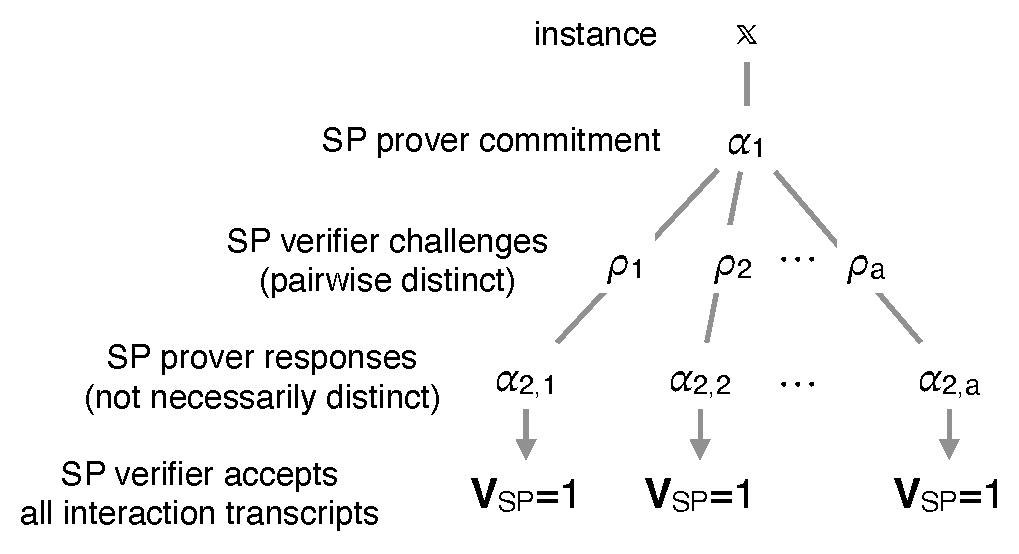
\includegraphics[width=0.6\textwidth]{\FigureFolder/fork-of-transcripts-diagram}
\caption{Diagram of an $\SSArity$-fork for an SP.}
\label{figure:fork-of-transcripts-diagram}
\end{figure}

\parhead{The case of public-coin IPs}
An IP is a multi-round protocol between a prover and a verifier (see \Cref{chapter:ip}). A public-coin IP has special soundness if a witness can be efficiently deduced from a \emph{tree} of accepting interaction transcripts for the given instance. This latter consists of a tree where vertices are labeled with IP prover messages, edges are labeled IP verifier messages, and every path from the root to a leaf is an accepting transcript; edges sharing the same vertex are labeled with pairwise distinct IP verifier messages. A list of parameters $\SSArity_{1},\dots,\SSArity_{\IPRoundComplexity} \in \Naturals$ determines the number of children that each vertex in the tree has, depending on the layer. See \Cref{figure:tree-of-transcripts-diagram} for a diagram.

\begin{definition}
\label{definition:ss-tree-structure}
Let $\SSArity_{1},\dots,\SSArity_{\IPRoundComplexity} \in \Naturals$. A \defemph{$(\SSArity_{1},\dots,\SSArity_{\IPRoundComplexity})$-tree} is a tree $\SSTree$ where:
\begin{inparaenum}[(1)]
  \item there are $\IPRoundComplexity+1$ layers, with layer $1$ being the root layer and layer $\IPRoundComplexity+1$ being the leaf layer;
  \item for every $\RoundIndex \in [\IPRoundComplexity]$, every vertex in layer $\RoundIndex$ has $\SSArity_{\RoundIndex}$ children.
\end{inparaenum}
In particular, the tree has $\prod_{\RoundIndex \in [\IPRoundComplexity]} \SSArity_{\RoundIndex}$ leaves.
\end{definition}

\begin{definition}
\label{definition:ss-tree-of-transcripts}
Let $\IPSymbol=\IPSystem$ be a public-coin IP with round complexity $\IPRoundComplexity$. Let $\SSArity_{1},\dots,\SSArity_{\IPRoundComplexity} \in \Naturals$ be arity parameters. A \defemph{$(\SSArity_{1},\dots,\SSArity_{\IPRoundComplexity})$-tree of transcripts for an instance $\Instance$} is a $(\SSArity_{1},\dots,\SSArity_{\IPRoundComplexity})$-tree $\SSTree$ that comes with vertex labels and edge labels that yield accepting transcripts:
\begin{inparaenum}[(1)]
  \item for every $\RoundIndex \in [\IPRoundComplexity]$, every vertex in layer $\RoundIndex$ is labeled with an IP prover message suitable for round $\RoundIndex$ (and the leaf vertices are unlabeled);
  \item for every $\RoundIndex \in [\IPRoundComplexity]$ and every vertex in layer $\RoundIndex$, the $\SSArity_{\RoundIndex}$ outgoing edges are labeled with distinct choices of IP verifier challenge suitable for round $\RoundIndex$; and
  \item every path from the root to a leaf corresponds to an accepting view for the IP verifier (on instance $\Instance$).
\end{inparaenum}
\end{definition}

\begin{definition}
\label{definition:ip-special-soundness}
Let $\IPSymbol=\IPSystem$ be a public-coin IP with round complexity $\IPRoundComplexity$. The IP $\IPSymbol$ has \defemph{special soundness with arity $(\SSArity_{1},\dots,\SSArity_{\IPRoundComplexity})$ with extraction time $\IPSSKnowledgeTime$} if there exists a deterministic algorithm $\IPSSExtractor$ such that, for every instance $\Instance$ and $(\SSArity_{1},\dots,\SSArity_{\IPRoundComplexity})$-tree $\SSTree$ of transcripts for $\Instance$, $\IPSSExtractor(\Instance,\SSTree)$ outputs $\Witness$ such that $(\Instance,\Witness) \in \Relation$ in time $\IPSSKnowledgeTime(\Instance)$.
\end{definition}

\begin{figure}[htp!]
\centering
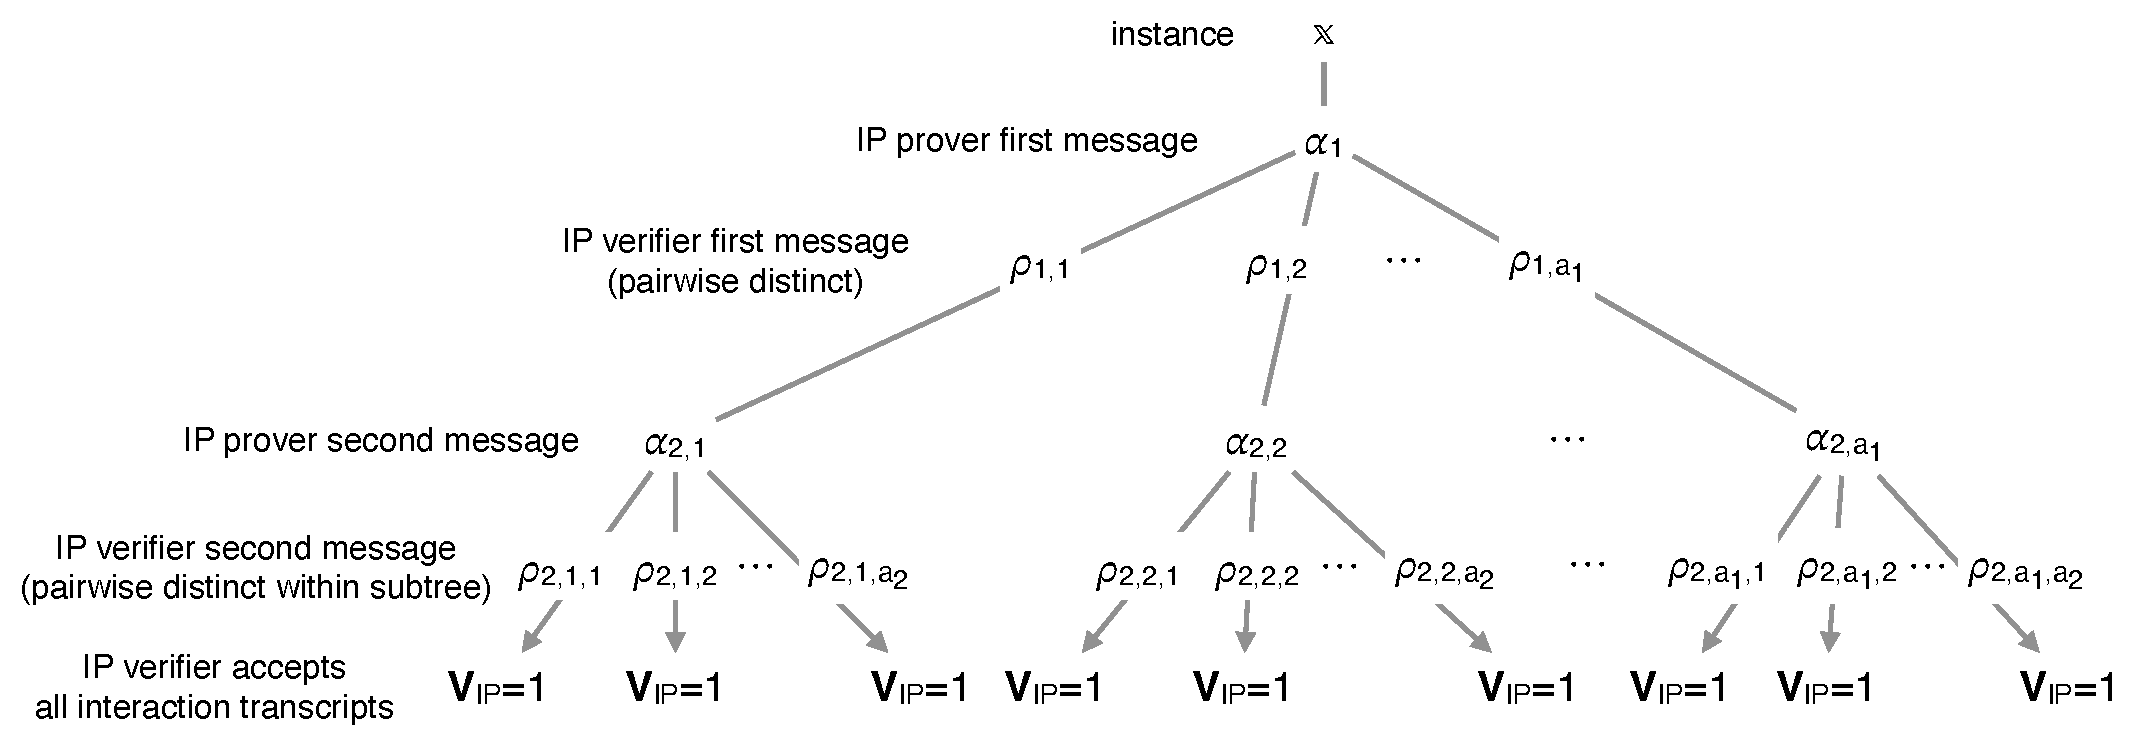
\includegraphics[width=0.95\textwidth]{\FigureFolder/tree-of-transcripts-diagram}
\caption{Diagram of an $(\SSArity_{1},\SSArity_{2})$-tree of transcripts for a public-coin IP.}
\label{figure:tree-of-transcripts-diagram}
\end{figure}

We also the define the notion of a \emph{subtree} of transcripts, which considers multiple accepting completions of a single partial transcript. The definition below generalizes \Cref{definition:ss-tree-of-transcripts} and, while not needed to define special soundness, we rely on it in various analyses in this chapter.

\begin{definition}
\label{definition:ss-subtree-of-transcripts}
For $j \in \{0,1,\dots,\IPRoundComplexity\}$, a \defemph{$(\SSArity_{j+1},\dots,\SSArity_{\IPRoundComplexity})$-subtree of transcripts for an instance $\Instance$ and partial IP transcript $((\IPProverMessage_{\RoundIndex})_{\RoundIndex=1}^{j},(\IPVerifierRandomMessage_{\RoundIndex})_{\RoundIndex=1}^{j})$} is a $(\SSArity_{j+1},\dots,\SSArity_{\IPRoundComplexity})$-tree $\SSTree$ that comes with vertex labels and edge labels that yield accepting transcripts:
\begin{inparaenum}[(1)]
  \item for every $\RoundIndex \in \{j+1,\dots,\IPRoundComplexity\}$, every vertex in layer $\RoundIndex-j$ is labeled with an IP prover message suitable for round $\RoundIndex$ (and the leaf vertices are unlabeled);
  \item for every $\RoundIndex \in \{j+1,\dots,\IPRoundComplexity\}$ and every vertex in layer $\RoundIndex-j$, the $\SSArity_{\RoundIndex}$ outgoing edges are labeled with distinct choices of IP verifier challenge suitable for round $\RoundIndex$; and
  \item every path from the root to a leaf completes the partial transcript $((\IPProverMessage_{\RoundIndex})_{\RoundIndex=1}^{j},(\IPVerifierRandomMessage_{\RoundIndex})_{\RoundIndex=1}^{j})$ into an accepting view for the IP verifier (on instance $\Instance$).
\end{inparaenum}
\end{definition}

\parhead{Negative hypergeometric distribution}
In this chapter, when analyzing certain probabilistic algorithms, the properties of the following distribution will be useful.

\begin{definition}
\label{definition:negative-hypergeometric-distribution}
The \defemph{negative hypergeometric distribution} describes the following probabilistic experiment. Elements are drawn one after another, without replacement, from a set of $\NHGTotalNumber$ elements out of which $\NHGGoodNumber$ are colored blue and the rest are colored red.

Let $\NHGSampledGood$ be the number of samples until $\NHGTargetNumber$ blue elements are drawn, and let $\NHGSampledBad$ be the number of red balls sampled. Then,
\begin{equation*}
\Pr[\NHGSampledGood=x] = \binom{x-1}{\NHGTargetNumber-1} \cdot \frac{\binom{\NHGTotalNumber-x}{\NHGGoodNumber-\NHGTargetNumber}}{\binom{\NHGTotalNumber}{\NHGGoodNumber}}
\text{ ,}\quad
\Expectation[\NHGSampledGood] = \frac{\NHGTargetNumber \cdot (\NHGTotalNumber+1)}{\NHGGoodNumber+1}
\text{ ,}\quad \text{and}\quad
\Expectation[\NHGSampledBad] \leq \frac{\NHGTargetNumber \cdot (\NHGTotalNumber-\NHGGoodNumber)}{\NHGGoodNumber+1}
\enspace.
\end{equation*}
\end{definition}

%%%%%%%%%%%%%%%%%%%%%%%%%%%%%%%%%%%%%%%%%%%%%%%%%%%%%%%%%%%%%%%%%%%%%%%%%%%%%%%
%%%%%%%%%%%%%%%%%%%%%%%%%%%%%%%%%%%%%%%%%%%%%%%%%%%%%%%%%%%%%%%%%%%%%%%%%%%%%%%
%%%%%%%%%%%%%%%%%%%%%%%%%%%%%%%%%%%%%%%%%%%%%%%%%%%%%%%%%%%%%%%%%%%%%%%%%%%%%%%
\section{Knowledge soundness for SPs}
\label{section:ss-sigma-protocols-knowledge}

We prove that if an SP has special soundness then the SP has rewinding knowledge soundness. The rewinding knowledge soundness error and extraction time increase as the arity of the special soundness increases; neither depends on the failure probability of the SP prover.

\begin{theorem}
\label{theorem:ss-to-knowledge-soundness-for-sp}
Let $\SPSymbol=\SPSystem$ be an SP with verifier randomness complexity $\SPRandomnessComplexity$. If $\SPSymbol$ has special soundness with arity $\SSArity$ with extraction time $\SPSSKnowledgeTime$ (see \Cref{definition:sp-special-soundness}) then $\SPSymbol$ has rewinding knowledge soundness error $\SPKnowledgeError$ with extraction time $\SPKnowledgeTime$ (see \Cref{definition:sp-knowledge-soundness}) such that
\begin{align*}
&\SPKnowledgeError(\Instance,\ProverFailureProbability{\SPMaliciousProver})
\leq
\frac{\SSArity - 1}{\SPRandomnessCardinality}
\enspace , \\
&\SPKnowledgeTime(\Instance,\ProverFailureProbability{\SPMaliciousProver},\ProverRunningTime{\SPMaliciousProver}) \leq (\SSArity-1) \cdot \left(\ProverRunningTime{\SPMaliciousProver} + \poly(\BitSize{\Instance})\right) + \SPSSKnowledgeTime(\Instance)
\enspace.
\end{align*}
\end{theorem}

Fix an instance $\Instance$ and SP prover $\SPMaliciousProver$. The main idea to prove the theorem is to rewind $\SPMaliciousProver$ several times with correlated inputs in order to obtain an $\SSArity$-fork $\SSFork$ for $\Instance$. This suffices because the knowledge extractor $\SPSSExtractor$ for special soundness can find a witness $\Witness$ from $\Instance$ and $\SSFork$.

The lemma below provides a probabilistic procedure $\SSForkFinder$ that outputs an $\SSArity$-fork $\SSFork$. The procedure $\SSForkFinder$ receives as input the instance $\Instance$, an interaction transcript $(\SPCommitment,\SPChallenge,\SPResponse)$ between the SP prover $\SPMaliciousProver$ and SP verifier $\SPVerifier$, and black-box access to $\SPMaliciousProver$. We describe how to upper bound the probability that $\SPMaliciousProver$ convinces $\SPVerifier$ and the output of $\SSForkFinder$ is not an $\SSArity$-fork $\SSFork$ for $\Instance$. Informally, $\SSForkFinder$ invokes $\SPMaliciousProver$ with different SP verifier challenges (but the same SP prover commitment) until it obtains $\SSArity-1$ additional accepting interaction transcripts. (The first accepting interaction transcript comes \DoQuote{for free} when the SP verifier $\SPVerifier$ accepts in the real interaction.)

\begin{lemma}
\label{lemma:ss-sp-to-knowledge-soundness}
The algorithm $\SSForkFinder$ in \Cref{construction:ss-fork-finder} satisfies the following property. For every SP prover $\SPMaliciousProver$ and instance $\Instance$,
\begin{equation*}
\Pr\left[
\begin{array}{l}
  \SSFork \text{ is not an $\SSArity$-fork for $\Instance$} \\
  \land\; \SPVerifier(\Instance,\SPCommitment,\SPChallenge,\SPResponse)=1
\end{array}
\GivenExperiment
\StateExperiment{
  (\SPCommitment,\AuxiliaryState) \gets \SPMaliciousProver \\
  \SPChallenge \gets \Bits^{\SPRandomnessComplexity} \\
  \SPResponse \gets \SPMaliciousProver(\AuxiliaryState,\SPChallenge) \\
  \SSFork \gets \SSForkFinder(\Instance,\SPCommitment,\SPChallenge,\SPResponse,\BlackBox{\SPMaliciousProver})
}
\right]
\leq
\frac{\SSArity-1}{\SPRandomnessCardinality}
\enspace.
\end{equation*}
Moreover, $\SSForkFinder$ runs in expected time $(\SSArity-1) \cdot \big(\ProverRunningTime{\SPMaliciousProver} + \poly(\BitSize{\Instance})\big)$.
\end{lemma}

\begin{construction}
\label{construction:ss-fork-finder}
The algorithm $\SSForkFinder$, given as input an instance $\Instance$, an SP interaction transcript $(\SPCommitment,\SPChallenge,\SPResponse)$, and black-box access to an SP prover $\SPMaliciousProver$, works as follows.
\begin{itemize}[noitemsep]
\item[] $\SSForkFinder(\Instance,\SPCommitment,\SPChallenge,\SPResponse,\BlackBox{\SPMaliciousProver})$:
\begin{enumerate}[nolistsep]
  \item \label{step:ss-fork-finder-early-abort}
  If $\SPVerifier(\Instance,\SPCommitment,\SPChallenge,\SPResponse)=0$ abort.
  \item Compute $\SPMaliciousProver$'s first message and intermediate state: $(\SPCommitment,\AuxiliaryState) \gets \SPMaliciousProver$.
  \item Set $\SSRemainingRandomness \DefineEqual \Bits^{\SPRandomnessComplexity} \setminus \{\SPChallenge\}$ and $\SSBranches \DefineEqual \{(\SPChallenge,\SPResponse)\}$.
  \item While $\SSRemainingRandomness$ is non-empty and $\Cardinality{\SSBranches} < \SSArity$:
  \begin{enumerate}[nolistsep]
    \item Sample an SP verifier challenge $\SPChallenge' \in \SSRemainingRandomness$, and remove $\SPChallenge'$ from $\SSRemainingRandomness$.
    \item \label{step:ss-fork-finder-invoke-sp-prover}
    Compute $\SPMaliciousProver$'s second message: $\SPResponse \gets \SPMaliciousProver(\AuxiliaryState,\SPChallenge')$.
    \item Compute the decision bit of the SP verifier: $b \gets \SPVerifier(\Instance,\SPCommitment,\SPChallenge',\SPResponse)$.
    \item If $b=1$ then add $(\SPChallenge',\SPResponse')$ to $\SSBranches$.
  \end{enumerate}
  \item If $\Cardinality{\SSBranches} < \SSArity$ then abort; else output $\SSFork \DefineEqual (\SPCommitment,\SSBranches)$.
\end{enumerate}
\end{itemize}
\end{construction}

\begin{proof}[Proof of \Cref{lemma:ss-sp-to-knowledge-soundness}]
We say that an SP verifier challenge $\SPChallenge \in \Bits^{\SPRandomnessComplexity}$ is \emph{good} for $(\Instance,\SPMaliciousProver)$ if $\SPVerifier(\Instance,\SPCommitment,\SPChallenge,\SPResponse)=1$, where $(\SPCommitment,\AuxiliaryState) \gets \SPMaliciousProver$ and $\SPResponse \gets \SPMaliciousProver(\AuxiliaryState,\SPChallenge)$. Denote by $\SSGoodChallengeNumber \in \{0,1,\dots,\SPRandomnessCardinality\}$ the number of SP verifier challenges in $\Bits^{\SPRandomnessComplexity}$ that are good for $(\Instance,\SPMaliciousProver)$. Denote by $\SSFinderHasFound \in \Bits$ the indicator for the event that $\SPChallenge$ (sampled in the experiment of the lemma statement) is good for $(\Instance,\SPMaliciousProver)$. By definition, for every $\ell \in \{0,1,\dots,\SPRandomnessCardinality\}$,
\begin{equation}
\label{equation:ss-fork-finder-good-probability}
\Pr\left[\SSFinderHasFound=1 \ConditionedOn \SSGoodChallengeNumber = \ell \right]
= \frac{\ell}{\SPRandomnessCardinality}
\enspace.
\end{equation}

\parhead{Error probability}
We upper bound the error probability of $\SSForkFinder$. The event in the probability in the lemma statement corresponds to $\SSFinderHasFound=1 \land \SSGoodChallengeNumber \leq \SSArity-1$. Indeed, provided that $\SPChallenge$ is good for $(\Instance,\SPMaliciousProver)$, $\SSForkFinder$ outputs an $\SSArity$-fork for $\Instance$ if and only if there are at least $\SSArity$ SP verifier challenges that are good for $(\Instance,\SPMaliciousProver)$. We upper bound the error probability as follows:
\begin{align*}
&\Pr\left[
\begin{array}{l}
  \SSFork \text{ is not an $\SSArity$-fork for $\Instance$}\\
  \land\;\SPVerifier(\Instance,\SPCommitment,\SPChallenge,\SPResponse)=1
\end{array}
\GivenExperiment
\StateExperiment{
  (\SPCommitment,\AuxiliaryState) \gets \SPMaliciousProver \\
  \SPChallenge \gets \Bits^{\SPRandomnessComplexity} \\
  \SPResponse \gets \SPMaliciousProver(\AuxiliaryState,\SPChallenge) \\
  \SSFork \gets \SSForkFinder(\Instance,\SPCommitment,\SPChallenge,\SPResponse,\BlackBox{\SPMaliciousProver})
}
\right] \\
&=\Pr\left[\SSFinderHasFound=1 \land \SSGoodChallengeNumber \leq \SSArity-1 \right] \\
&\leq \Pr\left[\SSFinderHasFound=1 \ConditionedOn \SSGoodChallengeNumber \leq \SSArity-1 \right] \\
&= \sum_{\ell=0}^{\SSArity-1} \Pr\left[\SSFinderHasFound=1 \ConditionedOn \SSGoodChallengeNumber=\ell \right] \cdot \Pr[\SSGoodChallengeNumber =\ell] \\
&= \sum_{\ell=0}^{\SSArity-1} \frac{\ell}{\SPRandomnessCardinality} \cdot \Pr[\SSGoodChallengeNumber =\ell] \EquationComment{by \Cref{equation:ss-fork-finder-good-probability}} \\
&\leq \frac{\SSArity-1}{\SPRandomnessCardinality} \cdot \sum_{\ell=0}^{\SSArity-1} \Pr[\SSGoodChallengeNumber =\ell] \\
&\leq \frac{\SSArity-1}{\SPRandomnessCardinality}
\enspace.
\end{align*}

\parhead{The while loop}
Let $\RandomVariableX$ be the number of times $\SSForkFinder$ enters the while loop. We argue that $\Expectation[\RandomVariableX] \leq \SSArity-1$. The expectation is over all randomness in the experiment: the SP verifier challenge $\SPChallenge$ and the internal randomness $\SSFinderRandomness$ of $\SSForkFinder$.

If $\SPChallenge$ is not good for $(\Instance,\SPMaliciousProver)$ then $\SSForkFinder$ aborts in \Cref{step:ss-fork-finder-early-abort}, so $\Expectation\left[\RandomVariableX \ConditionedOn \SSFinderHasFound=0 \right]=0$. If instead $\SPChallenge$ is good for $(\Instance,\SPMaliciousProver)$ then $\SSForkFinder$ reaches the while loop. We argue that, for every $\ell \in \{1,\dots,\SPRandomnessCardinality\}$,
\begin{equation}
\label{equation:ss-fork-finder-number-while-iterations}
\Expectation\left[\RandomVariableX \ConditionedOn \SSFinderHasFound = 1 \land \SSGoodChallengeNumber = \ell \right] \leq \frac{(\SSArity-1) \cdot \SPRandomnessCardinality}{\ell}
\enspace.
\end{equation}
We consider two cases.
\begin{itemize}

  \item If $\ell < \SSArity$ then $\SSForkFinder$ enters the while loop $\SPRandomnessCardinality-1$ times and then aborts (there are not enough good SP verifier challenges). Hence, $\Expectation\left[\RandomVariableX \ConditionedOn \SSGoodChallengeNumber = \ell \right] = \SPRandomnessCardinality-1 = \frac{\ell \cdot (\SPRandomnessCardinality-1)}{\ell} \leq \frac{(\SSArity-1) \cdot (\SPRandomnessCardinality-1)}{\ell} < \frac{(\SSArity-1) \cdot \SPRandomnessCardinality}{\ell}$.

  \item If $\ell \geq \SSArity$ then $\SSForkFinder$ enters the while loop until it finds $\SSArity-1$ SP verifier challenges that are good for $(\Instance,\SPMaliciousProver)$. Specifically, $\SSForkFinder$ samples without replacement from a set of cardinality $\SPRandomnessCardinality-1$ until it obtains $\SSArity-1$ \DoQuote{successes}. Therefore, $\RandomVariableX$ follows the random variable $\NHGSampledGood$ defined for the negative hypergeometric distribution (see \Cref{definition:negative-hypergeometric-distribution}) with a set size $\SPRandomnessCardinality-1$, a total of $\ell-1$ blue elements, and a target of $\SSArity-1$ blue elements. Hence the expected number of times $\SSForkFinder$ enters the while loop is $\Expectation\left[\RandomVariableX \ConditionedOn \SSGoodChallengeNumber = \ell \right] = \frac{(\SSArity-1) \cdot \SPRandomnessCardinality}{\ell}$.

\end{itemize}
Therefore, by the total expectation theorem,
\begin{align*}
&\Expectation[\RandomVariableX] \\
&= \Expectation\left[\RandomVariableX \ConditionedOn \SSFinderHasFound=0 \right] \cdot \Pr[\SSFinderHasFound=0] + \Expectation\left[\RandomVariableX \ConditionedOn \SSFinderHasFound=1 \right] \cdot \Pr[\SSFinderHasFound=1] \\
&= 0 + \Expectation\left[\RandomVariableX \ConditionedOn \SSFinderHasFound=1 \right] \cdot \Pr[\SSFinderHasFound=1] \\
&= \sum_{\ell=1}^{\SPRandomnessCardinality} \Expectation\left[\RandomVariableX \ConditionedOn \SSFinderHasFound=1 \land \SSGoodChallengeNumber = \ell \right] \cdot \Pr[\SSFinderHasFound=1 \land \SSGoodChallengeNumber=\ell] \EquationComment{$\SSFinderHasFound=1$ implies $\SSGoodChallengeNumber>0$} \\
&\leq \sum_{\ell=1}^{\SPRandomnessCardinality} \frac{(\SSArity-1) \cdot \SPRandomnessCardinality}{\ell} \cdot \Pr[\SSFinderHasFound=1 \land \SSGoodChallengeNumber = \ell] \EquationComment{by \Cref{equation:ss-fork-finder-number-while-iterations}} \\
&= \sum_{\ell=1}^{\SPRandomnessCardinality} \frac{(\SSArity-1) \cdot \SPRandomnessCardinality}{\ell} \cdot \Pr\left[\SSFinderHasFound=1 \ConditionedOn \SSGoodChallengeNumber = \ell \right] \cdot \Pr[\SSGoodChallengeNumber = \ell] \\
&= \sum_{\ell=1}^{\SPRandomnessCardinality} \frac{(\SSArity-1) \cdot \SPRandomnessCardinality}{\ell} \cdot \frac{\ell}{\SPRandomnessCardinality} \cdot \Pr[\SSGoodChallengeNumber = \ell] \EquationComment{by \Cref{equation:ss-fork-finder-good-probability}} \\
& =
(\SSArity-1) \cdot \sum_{\ell=1}^{\SPRandomnessCardinality} \Pr[\SSGoodChallengeNumber = \ell]
= \SSArity-1
\enspace.
\end{align*}

\parhead{Running time}
We analyze the expected running time of $\SSForkFinder$. First we analyze how $\SSForkFinder$ invokes $\SPMaliciousProver$. The algorithm $\SSForkFinder$ computes a first message of $\SPMaliciousProver$ in \Cref{step:ss-fork-finder-early-abort}; this is the only time $\SSForkFinder$ computes a first message of $\SPMaliciousProver$. Moreover, $\SSForkFinder$ computes a second message of $\SPMaliciousProver$ every time $\SSForkFinder$ executes the while loop, in \Cref{step:ss-fork-finder-invoke-sp-prover}. In expectation this happens $\Expectation[\RandomVariableX] \leq \SSArity-1$ times. Overall, since $\ProverRunningTime{\SPMaliciousProver}$ denotes the total running time of $\SPMaliciousProver$ (i.e., the running time to compute the first and the second message), the total time spent by $\SSForkFinder$ invoking $\SPMaliciousProver$ is upper bounded by $(\SSArity-1) \cdot \ProverRunningTime{\SPMaliciousProver}$. All other operations in $\SSForkFinder$ take time $\poly(\BitSize{\Instance})$, which in expectation across all while loop iterations add up to time $(\SSArity-1) \cdot \poly(\BitSize{\Instance})$.
\end{proof}

\begin{construction}
\label{construction:ss-extractor-for-sp}
Let $\SPSSExtractor$ be the special soundness extractor for $\SPSymbol$, and let $\SSForkFinder$ be the algorithm in \Cref{construction:ss-fork-finder}. The rewinding knowledge extractor $\SPExtractor$ receives as input an instance $\Instance$, an interaction transcript $(\SPCommitment,\SPChallenge,\SPResponse)$, and black-box access to an SP prover $\SPMaliciousProver$, and works as follows.
\begin{itemize}[noitemsep]
\item[] $\SPExtractor(\Instance,\SPCommitment,\SPChallenge,\SPResponse,\BlackBox{\SPMaliciousProver})$:
\begin{enumerate}[nolistsep]
  \item Run $\SSFork \gets \SSForkFinder(\Instance,\SPCommitment,\SPChallenge,\SPResponse,\BlackBox{\SPMaliciousProver})$; if $\SSForkFinder$ aborts then abort.
  \item Run $\Witness \gets \SPSSExtractor(\Instance,\SSFork)$.
  \item Output $\Witness$.
\end{enumerate}
\end{itemize}
\end{construction}

\begin{proof}[Proof of \Cref{theorem:ss-to-knowledge-soundness-for-sp}]
The knowledge extractor $\SPExtractor$ succeeds if the algorithm $\SSForkFinder$ succeeds, so the knowledge soundness error of $\SPExtractor$ is at most the failure probability of $\SSForkFinder$. This latter, by \Cref{lemma:ss-sp-to-knowledge-soundness}, is at most $\frac{\SSArity-1}{\SPRandomnessCardinality}$. Hence the knowledge soundness error of $\SPExtractor$ is as claimed in \Cref{theorem:ss-to-knowledge-soundness-for-sp}.

Moreover, the expected running time of $\SPExtractor$ is the expected running time of $\SSForkFinder$ plus the running time of $\SPSSExtractor$. By \Cref{lemma:ss-sp-to-knowledge-soundness}, the expected running time of $\SSForkFinder$ is at most $(\SSArity-1) \cdot \big(\ProverRunningTime{\SPMaliciousProver} + \poly(\BitSize{\Instance})\big)$. By definition, the running time of $\SPSSExtractor$ is $\SPSSKnowledgeTime(\Instance)$. We conclude that the expected running time of $\SPExtractor$ is as claimed in \Cref{theorem:ss-to-knowledge-soundness-for-sp}.
\end{proof}

%%%%%%%%%%%%%%%%%%%%%%%%%%%%%%%%%%%%%%%%%%%%%%%%%%%%%%%%%%%%%%%%%%%%%%%%%%%%%%%
%%%%%%%%%%%%%%%%%%%%%%%%%%%%%%%%%%%%%%%%%%%%%%%%%%%%%%%%%%%%%%%%%%%%%%%%%%%%%%%
%%%%%%%%%%%%%%%%%%%%%%%%%%%%%%%%%%%%%%%%%%%%%%%%%%%%%%%%%%%%%%%%%%%%%%%%%%%%%%%
\section{State-restoration knowledge soundness for SPs}
\label{section:ss-sigma-protocols-sr-knowledge}

We prove that if an SP has special soundness then the SP has rewinding \emph{state-restoration} knowledge soundness. The rewinding state-restoration knowledge soundness error and extraction time increase as the arity of the special soundness increases; neither depends on the failure probability of the state-restoration SP prover.

\begin{theorem}
\label{theorem:ss-to-sr-knowledge-soundness-for-sp}
Let $\SPSymbol=\SPSystem$ be an SP with verifier randomness complexity $\SPRandomnessComplexity$. If $\SPSymbol$ has special soundness with arity $\SSArity$ with extraction time $\SPSSKnowledgeTime$ (see \Cref{definition:sp-special-soundness}) then $\SPSymbol$ has rewinding state-restoration knowledge soundness error $\SPSRKnowledgeError$ with extraction time $\SPSRKnowledgeTime$ (see \Cref{definition:sp-state-restoration-knowledge}) such that
\begin{align*}
&\SPSRKnowledgeError(\SRSaltSize,\SRBudget,\InstanceSize,\ProverFailureProbability{\SPMaliciousSRProver})
\leq
(\SRBudget+1) \cdot \frac{\SSArity - 1}{\SPRandomnessCardinality}
\enspace, \\
&\SPSRKnowledgeTime(\SRSaltSize,\SRBudget,\InstanceSize,\ProverFailureProbability{\SPMaliciousSRProver},\ProverRunningTime{\SPMaliciousSRProver}) \leq (\SRBudget+1) \cdot (\SSArity-1) \cdot \left(\ProverRunningTime{\SPMaliciousSRProver} + \poly(\BitSize{\Instance})\right) + \SPSSKnowledgeTime(\Instance)
\enspace.
\end{align*}
\end{theorem}

The proof of this theorem is similar to the proof of \Cref{theorem:ss-to-knowledge-soundness-for-sp}: rewind the given SP state-restoration prover $\SPMaliciousSRProver$ several times with correlated inputs in order to obtain an $\SSArity$-fork $\SSFork$ for the instance $\Instance$; this suffices because the knowledge extractor $\SPSSExtractor$ for special soundness can find a witness $\Witness$ from $\Instance$ and $\SSFork$. However, there are notable differences that make the proof more technical. First, in rewinding state-restoration knowledge soundness (\Cref{definition:sp-state-restoration-knowledge}), the SP state-restoration prover $\SPMaliciousSRProver$ chooses the instance $\Instance$ in the SP state-restoration game; in contrast, in rewinding knowledge soundness (\Cref{definition:sp-knowledge-soundness}) the instance $\Instance$ is fixed. Moreover, the SP state-restoration prover $\SPMaliciousSRProver$ can make multiple attempts at convincing the SP verifier, not only with different instances but also with different SP commitments; this complicates the rewinding strategy.

The lemma below provides a probabilistic procedure $\SSSRForkFinder$ that outputs an $\SSArity$-fork $\SSFork$, which is analogous to \Cref{lemma:ss-sp-to-knowledge-soundness}. The procedure $\SSSRForkFinder$ receives as input the output $(\Instance,\SPCommitment,\SRSaltString,\SPChallenge,\SPResponse)$ of the SP state-restoration game played by $\SPMaliciousSRProver$, the list of move-response pairs $\SRTrace$ of $\SPMaliciousSRProver$, and black-box access to $\SPMaliciousSRProver$. The main challenge is that each time $\SSSRForkFinder$ reruns $\SPMaliciousSRProver$ we get a new output whose instance and first SP prover message may not agree with those received as input, which would not contribute progress towards the desired $\SSArity$-fork for $\Instance$.\footnote{This is not an issue in the proof of \Cref{lemma:ss-sp-to-knowledge-soundness} because there $\SSForkFinder$ can rerun only the part of the SP prover $\SPMaliciousProver$ corresponding to the second round.} Informally, $\SSSRForkFinder$ identifies the first move (if any) corresponding to $(\Instance,\SPCommitment,\SRSaltString)$, and then reruns $\SPMaliciousSRProver$ with freshly sampled answers (consistently answering other moves as needed) until enough accepting SP interaction transcripts with the same instance and SP prover message are found. Intuitively, this takes a multiplicative factor $(\SRBudget+1)$ more reruns compared to \Cref{lemma:ss-sp-to-knowledge-soundness}, as $\SPMaliciousSRProver$ makes at most $\SRBudget$ moves and can also output something corresponding to no move. Analyzing the success probability and expected running time of $\SSSRForkFinder$ is more technical, and the simpler analysis for \Cref{lemma:ss-sp-to-knowledge-soundness} is as a useful warmup.

\begin{lemma}
\label{lemma:ss-sp-to-sr-knowledge-soundness}
The algorithm $\SSSRForkFinder$ in \Cref{construction:ss-sr-fork-finder} satisfies the following property. For every SP state-restoration prover $\SPMaliciousSRProver$ that makes at most $\SRBudget$ moves,
\begin{align*}
& \Pr\left[
\begin{array}{l}
  \SomeSize{\Instance} \leq \InstanceSize \\
  \land\;\SSFork \text{ is not an $\SSArity$-fork for $\Instance$} \\
  \land\;\SPVerifier(\Instance,\SPCommitment,\SPChallenge,\SPResponse)=1
\end{array}
\GivenExperiment
\StateExperiment{
  \SRRandomness \gets \RODistribution{\SPRandomnessComplexity} \\
  (\Instance,\SPCommitment,\SRSaltString,\SPChallenge,\SPResponse) \xleftarrow{\SRTrace}\SPStateRestorationGame{\SRSaltSize}{\SRRandomness}{\SPMaliciousSRProver} \\
  \SSFork \gets \SSSRForkFinder(\Instance,\SPCommitment,\SRSaltString,\SPChallenge,\SPResponse,\SRTrace,\BlackBox{\SPMaliciousSRProver})
}
\right] \\
& \leq (\SRBudget+1) \cdot \frac{\SSArity - 1}{\SPRandomnessCardinality}
\enspace.
\end{align*}
Moreover, $\SSSRForkFinder$ runs in expected time $(\SRBudget+1) \cdot (\SSArity-1) \cdot \big(\ProverRunningTime{\SPMaliciousSRProver} + \poly(\BitSize{\Instance})\big)$.
\end{lemma}

\begin{construction}
\label{construction:ss-sr-fork-finder}
The algorithm $\SSSRForkFinder$, given as input a game output $(\Instance,\SPCommitment,\SRSaltString,\SPChallenge,\SPResponse)$ of the SP state-restoration game, a move-response trace $\SRTrace$, and black-box access to an SP state-restoration prover $\SPMaliciousSRProver$, works as follows.
\begin{itemize}
\item[] $\SSSRForkFinder(\Instance,\SPCommitment,\SRSaltString,\SPChallenge,\SPResponse,\SRTrace,\BlackBox{\SPMaliciousSRProver})$:
\begin{enumerate}[nolistsep]
  \item \label{step:ss-sr-fork-finder-early-abort}
  If $\SPVerifier(\Instance,\SPCommitment,\SPChallenge,\SPResponse)=0$ or $\SomeSize{\Instance} > \InstanceSize$, abort.
  \item \label{step:ss-sr-fork-finder-append-last-move-response}
  If the move-response pair $((\Instance,\SPCommitment,\SRSaltString),\SPChallenge)$ is not in $\SRTrace$ then append it to $\SRTrace$.
  \item Lazily sample an oracle $\LazySRRandomness \gets \RODistribution{\SPRandomnessComplexity}$ that is consistent with the move-response trace $\SRTrace$. (Lazily sample an oracle $\LazySRRandomness' \gets \RODistribution{\SPRandomnessComplexity}$ and program the oracle $\LazySRRandomness \DefineEqual \ROProgram{\LazySRRandomness'}{\SRTrace}$.)
  \item Set $\SSRemainingRandomness \DefineEqual \Bits^{\SPRandomnessComplexity} \setminus \{\SPChallenge\}$ and $\SSBranches \DefineEqual \{(\SPChallenge,\SPResponse)\}$.
  \item While $\SSRemainingRandomness$ is non-empty and $\Cardinality{\SSBranches} < \SSArity$:
  \begin{enumerate}[nolistsep]
    \item Sample an SP verifier challenge $\SPChallenge' \in \SSRemainingRandomness$, and remove $\SPChallenge'$ from $\SSRemainingRandomness$.
    \item Set $\ProgrammedList \DefineEqual \{((\Instance,\SPCommitment,\SRSaltString),\SPChallenge')\}$.
    \item \label{step:ss-sr-fork-finder-run-sp-sr-prover}
    Run the SP state-restoration game: $(\Instance',\SPCommitment',\SRSaltString',\SPChallenge',\SPResponse') \gets \SPStateRestorationGame{\SRSaltSize}{\ROProgram{\LazySRRandomness}{\ProgrammedList}}{\SPMaliciousSRProver}$.
    \item Compute the decision bit of the SP verifier: $\DecisionBit \gets \SPVerifier(\Instance',\SPCommitment',\SPChallenge',\SPResponse')$.
    \item If $\DecisionBit=1 \land \Instance'=\Instance \land \SPCommitment' = \SPCommitment$ then add $(\SPChallenge',\SPResponse')$ to $\SSBranches$.
  \end{enumerate}
  \item If $\Cardinality{\SSBranches} < \SSArity$ then abort; else output $\SSFork \DefineEqual (\SPCommitment,\SSBranches)$.
\end{enumerate}
\end{itemize}
The above description creates some redundant computation: the moves of $\SPMaliciousSRProver$ in every run of the SP state-restoration game $\SPStateRestorationGame{\SRSaltSize}{\ROProgram{\LazySRRandomness}{\ProgrammedList}}{\SPMaliciousSRProver}$ are the same up to the first move that equals $(\Instance,\SPCommitment,\SRSaltString)$ (if any); hence, this part of the game could be emulated before the while loop, and the remaining part of the game could be emulated in each while loop (each time with a different answer).
\end{construction}


\begin{proof}[Proof of \Cref{lemma:ss-sp-to-sr-knowledge-soundness}]
Fix any state-restoration randomness $\SRRandomness$, instance $\Instance$, SP prover commitment $\SPCommitment$, and salt $\SRSaltString$. We say that $\SPChallenge \in \Bits^{\SPRandomnessComplexity}$ is \emph{good} for $(\SRRandomness,\Instance,\SPCommitment,\SRSaltString)$ if there exists an SP prover response $\SPResponse$ such that:
\begin{enumerate}[noitemsep]
  \item $\SomeSize{\Instance} \leq \InstanceSize$;
  \item $\SPVerifier(\Instance,\SPCommitment,\SPChallenge,\SPResponse)=1$; and
  \item The output of $\SPStateRestorationGame{\SRSaltSize}{\ROProgram{\SRRandomness}{\ProgrammedList}}{\SPMaliciousSRProver}$ is $(\Instance,\SPCommitment,\SRSaltString,\SPChallenge,\SPResponse)$ where $\ProgrammedList = \{((\Instance,\SPCommitment,\SRSaltString),\SPChallenge)\}$. (The notation $\ROProgram{\SRRandomness}{\ProgrammedList}$ denotes the function $\SRRandomness$ re-programmed with the pairs in $\ProgrammedList$.)
\end{enumerate}
Additionally, define $\SSGoodChallengeNumber_{\SRRandomness,\Instance,\SPCommitment,\SRSaltString} \in \{0,1,\dots,\SPRandomnessCardinality\}$ to be the number of SP verifier challenges $\SPChallenge \in \Bits^{\SPRandomnessComplexity}$ that are good for $(\SRRandomness,\Instance,\SPCommitment,\SRSaltString)$; we write $\SSGoodChallengeNumber$ (without subscripts) to refer to $\SSGoodChallengeNumber_{\SRRandomness,\Instance,\SPCommitment,\SRSaltString}$ where $\SRRandomness$ is the randomness for the SP state-restoration game and $(\Instance,\SPCommitment,\SRSaltString)$ are in the output of the SP state-restoration game.

Let $\SSSRMoveSet \DefineEqual \{(\Instance',\SPCommitment',\SRSaltString') : \SomeSize{\Instance'} \leq \InstanceSize, \SPCommitment' \in \Bits^{\SPPToVComplexity_{1}}, \SRSaltString' \in \Bits^{\SRSaltSize}\}$. We show that
\begin{equation}
\label{eq:sum-convincing-number}
\sum_{(\Instance',\SPCommitment',\SRSaltString') \in \SSSRMoveSet}
\Pr\left[
  \SSGoodChallengeNumber_{\SRRandomness,\Instance',\SPCommitment',\SRSaltString'} > 0
\GivenExperiment
\StateExperiment{
  \SRRandomness \gets \RODistribution{\SPRandomnessComplexity}
}
\right]
\leq \SRBudget + 1
\enspace.
\end{equation}

For every $\SRRandomness \in \RODistribution{\SPRandomnessComplexity}$, define $S(\SRRandomness)$ to be the set of unique moves (i.e., no duplicates) performed by $\SPMaliciousSRProver$ in the SP state-restoration game $\SPStateRestorationGame{\SRSaltSize}{\SRRandomness}{\SPMaliciousSRProver}$; the set $S(\SRRandomness)$ also includes the move $(\Instance,\SPCommitment,\SRSaltString)$ contained in the output of the game in case $\SPMaliciousSRProver$ did not make this move. Note that $\Cardinality{S(\SRRandomness)} \leq \SRBudget+1$. Moreover, for every $(\Instance',\SPCommitment',\SRSaltString') \notin S(\SRRandomness)$ and $\SPChallenge \in \Bits^{\SPRandomnessComplexity}$, programming $\SRRandomness$ with $\ProgrammedList = \{((\Instance',\SPCommitment',\SRSaltString'),\SPChallenge)\}$ does not change the output of the SP state-restoration game, i.e., the output of $\SPStateRestorationGame{\SRSaltSize}{\ROProgram{\SRRandomness}{\ProgrammedList}}{\SPMaliciousSRProver}$ equals that of $\SPStateRestorationGame{\SRSaltSize}{\SRRandomness}{\SPMaliciousSRProver}$. We argue that if $(\Instance',\SPCommitment',\SRSaltString') \notin S(\SRRandomness)$ then $\SSGoodChallengeNumber_{\SRRandomness,\Instance',\SPCommitment',\SRSaltString'} = 0$. Indeed, suppose by way of contradiction that $\SSGoodChallengeNumber_{\SRRandomness,\Instance',\SPCommitment',\SRSaltString'} > 0$, which means that there exists an SP verifier challenge $\SPChallenge \in \Bits^{\SPRandomnessComplexity}$ that is good for $(\SRRandomness,\Instance',\SPCommitment',\SRSaltString')$, which in turn means that, for $\ProgrammedList = \{((\Instance',\SPCommitment',\SRSaltString'),\SPChallenge)\}$, the output of $\SPStateRestorationGame{\SRSaltSize}{\ROProgram{\SRRandomness}{\ProgrammedList}}{\SPMaliciousSRProver}$ contains $(\Instance',\SPCommitment',\SRSaltString')$; since $(\Instance',\SPCommitment',\SRSaltString') \notin S(\SRRandomness)$, the output of $\SPStateRestorationGame{\SRSaltSize}{\ROProgram{\SRRandomness}{\ProgrammedList}}{\SPMaliciousSRProver}$ equals that of $\SPStateRestorationGame{\SRSaltSize}{\SRRandomness}{\SPMaliciousSRProver}$, which lets us conclude that $(\Instance',\SPCommitment',\SRSaltString') \in S(\SRRandomness)$, a contradiction.

This allows us to prove \Cref{eq:sum-convincing-number} as follows:
\begin{align*}
& \sum_{(\Instance',\SPCommitment',\SRSaltString') \in \SSSRMoveSet} \Pr\left[\SSGoodChallengeNumber_{\SRRandomness,\Instance',\SPCommitment',\SRSaltString'} > 0
\GivenExperiment
\StateExperiment{
  \SRRandomness \gets \RODistribution{\SPRandomnessComplexity}
}
\right]
\\ & =
\sum_{(\Instance',\SPCommitment',\SRSaltString') \in \SSSRMoveSet}
\sum_{\SRRandomness' \in \RODistribution{\SPRandomnessComplexity}}
\Pr\left[\SSGoodChallengeNumber_{\SRRandomness',\Instance',\SPCommitment',\SRSaltString'} > 0
\right]
\cdot
\Pr\left[
\SRRandomness = \SRRandomness'
\GivenExperiment
\StateExperiment{
  \SRRandomness \gets \RODistribution{\SPRandomnessComplexity}
}
\right]
\\ & =
\sum_{\SRRandomness' \in \RODistribution{\SPRandomnessComplexity}}
\Pr\left[
\SRRandomness = \SRRandomness'
\GivenExperiment
\StateExperiment{
  \SRRandomness \gets \RODistribution{\SPRandomnessComplexity}
}
\right]
\sum_{(\Instance',\SPCommitment',\SRSaltString') \in \SSSRMoveSet}
\Pr\left[\SSGoodChallengeNumber_{\SRRandomness',\Instance',\SPCommitment',\SRSaltString'} > 0
\right]
\\ & =
\sum_{\SRRandomness' \in \RODistribution{\SPRandomnessComplexity}}
\Pr\left[
\SRRandomness = \SRRandomness'
\GivenExperiment
\StateExperiment{
  \SRRandomness \gets \RODistribution{\SPRandomnessComplexity}
}
\right] \cdot
\sum_{(\Instance',\SPCommitment',\SRSaltString') \in S(\SRRandomness')}
\Pr\left[
\SSGoodChallengeNumber_{\SRRandomness',\Instance',\SPCommitment',\SRSaltString'} > 0
\right]
\\ & \leq
\sum_{\SRRandomness' \in \RODistribution{\SPRandomnessComplexity}}
\Pr\left[
\SRRandomness = \SRRandomness'
\GivenExperiment
\StateExperiment{
  \SRRandomness \gets \RODistribution{\SPRandomnessComplexity}
}
\right] \cdot
(\SRBudget+1)
\\ & =
(\SRBudget+1) \cdot
\sum_{\SRRandomness' \in \RODistribution{\SPRandomnessComplexity}}
\Pr\left[
\SRRandomness = \SRRandomness'
\GivenExperiment
\StateExperiment{
  \SRRandomness \gets \RODistribution{\SPRandomnessComplexity}
}
\right]
\\ & =
\SRBudget+1
\enspace.
\end{align*}
Above, for a fixed $\SRRandomness'$, the probability $\Pr[\SSGoodChallengeNumber_{\SRRandomness',\Instance',\SPCommitment',\SRSaltString'} > 0]$ is $0$ or $1$, but it is convenient to use the probability notation.

Denote by $\SSFinderHasFound_{\SRRandomness,\Instance,\SPCommitment,\SRSaltString,\SPChallenge} \in \Bits$ the indicator for the event that $\SPChallenge$ is good for $(\SRRandomness,\Instance,\SPCommitment,\SRSaltString)$; we write $\SSFinderHasFound$ (without subscripts) to refer to $\SSFinderHasFound_{\SRRandomness,\Instance,\SPCommitment,\SRSaltString,\SPChallenge}$ where $\SRRandomness$ is the randomness for the SP state-restoration game and $(\Instance,\SPCommitment,\SRSaltString,\SPChallenge)$ are in the output of the SP state-restoration game.

For every $(\Instance',\SPCommitment',\SRSaltString') \in \SSSRMoveSet$ and $\ell \in \{0,1,\dots,\SPRandomnessCardinality\}$, we argue that
\begin{equation}
\label{equation:ss-sp-to-sr-probability-of-good}
\Pr\left[
\begin{array}{l}
  \SSFinderHasFound_{\SRRandomness,\Instance,\SPCommitment,\SRSaltString,\SPChallenge}=1 \\
  \land\;(\Instance,\SPCommitment,\SRSaltString)=(\Instance',\SPCommitment',\SRSaltString') \\
 \ConditionedOnText \\
  \SSGoodChallengeNumber_{\SRRandomness,\Instance,\SPCommitment,\SRSaltString} = \ell
\end{array}
\GivenExperiment
\StateExperiment{
  \SRRandomness \gets \RODistribution{\SPRandomnessComplexity} \\
  \ShortExecution
  {(\Instance,\SPCommitment,\SRSaltString,\SPChallenge,\SPResponse)}
  {\SPStateRestorationGame{\SRSaltSize}{\SRRandomness}{\SPMaliciousSRProver}}
}
\right]
=
\frac{\ell}{\SPRandomnessCardinality}
\enspace.
\end{equation}
First suppose that $\ell=0$: if $\SSGoodChallengeNumber_{\SRRandomness,\Instance,\SPCommitment,\SRSaltString}=0$ then $\SSFinderHasFound_{\SRRandomness,\Instance,\SPCommitment,\SRSaltString,\SPChallenge}=0$, so the probability equals $0$ in this case. Next, if $\ell \in \{1,\dots,\SPRandomnessCardinality\}$, we argue as follows:
\begin{align*}
& \Pr\left[
\begin{array}{l}
  \SSFinderHasFound_{\SRRandomness,\Instance,\SPCommitment,\SRSaltString,\SPChallenge}=1 \\
  \land\;(\Instance,\SPCommitment,\SRSaltString)=(\Instance',\SPCommitment',\SRSaltString') \\
  \ConditionedOnText \\
  \SSGoodChallengeNumber_{\SRRandomness,\Instance,\SPCommitment,\SRSaltString} = \ell
\end{array}
\GivenExperiment
\StateExperiment{
  \SRRandomness \gets \RODistribution{\SPRandomnessComplexity} \\
  \ShortExecution
  {(\Instance,\SPCommitment,\SRSaltString,\SPChallenge,\SPResponse)}
  {\SPStateRestorationGame{\SRSaltSize}{\SRRandomness}{\SPMaliciousSRProver}}
}
\right]
\\ & =
\Pr\left[
\begin{array}{l}
  \SSFinderHasFound_{\SRRandomness,\Instance',\SPCommitment',\SRSaltString',\SPChallenge'}=1 \\
  \land\;(\Instance,\SPCommitment,\SRSaltString)=(\Instance',\SPCommitment',\SRSaltString') \\
  \ConditionedOnText \\
  \SSGoodChallengeNumber_{\SRRandomness,\Instance',\SPCommitment',\SRSaltString'} = \ell
\end{array}
\GivenExperiment
\StateExperiment{
  \SRRandomness \gets \RODistribution{\SPRandomnessComplexity} \\
  \ShortExecution
  {(\Instance,\SPCommitment,\SRSaltString,\SPChallenge,\SPResponse)}
  {\SPStateRestorationGame{\SRSaltSize}{\SRRandomness}{\SPMaliciousSRProver}} \\
  \SPChallenge' \DefineEqual \SRRandomness(\Instance',\SPCommitment',\SRSaltString')
}
\right]
\\ & =
\Pr\left[
\begin{array}{l}
  \SSFinderHasFound_{\SRRandomness,\Instance',\SPCommitment',\SRSaltString',\SPChallenge'}=1 \\
  \ConditionedOnText \\
  \SSGoodChallengeNumber_{\SRRandomness,\Instance',\SPCommitment',\SRSaltString'} = \ell
\end{array}
\GivenExperiment
\StateExperiment{
  \SRRandomness \gets \RODistribution{\SPRandomnessComplexity} \\
  \SPChallenge' \DefineEqual \SRRandomness(\Instance',\SPCommitment',\SRSaltString')
}
\right]
=
\frac{\ell}{\SPRandomnessCardinality}
\enspace.
\end{align*}
Above, the second equality holds because the condition $\SSGoodChallengeNumber_{\SRRandomness,\Instance',\SPCommitment',\SRSaltString'} = \ell > 0$ implies that $(\Instance',\SPCommitment',\SRSaltString')$ is part of the output of the state-restoration game and thus $(\Instance,\SPCommitment,\SRSaltString)=(\Instance',\SPCommitment',\SRSaltString')$.

\parhead{Error probability}
We upper bound the error probability of $\SSSRForkFinder$. The event in the probability in the lemma statement implies the event $\SSFinderHasFound=1 \land \SSGoodChallengeNumber \leq \SSArity-1$, that is, $\SSFinderHasFound_{\SRRandomness,\Instance,\SPCommitment,\SRSaltString,\SPChallenge}=1 \land \SSGoodChallengeNumber_{\SRRandomness,\Instance,\SPCommitment,\SRSaltString} \leq \SSArity-1$ where $\SRRandomness$ is the randomness for the SP state-restoration game and $(\Instance,\SPCommitment,\SRSaltString,\SPChallenge)$ are in the output of the SP state-restoration game. Indeed, the conditions $\SomeSize{\Instance} \leq \InstanceSize$ and $\SPVerifier(\Instance,\SPCommitment,\SPChallenge,\SPResponse)=1$ imply that $\SSFinderHasFound=1$ and the condition that $\SSFork \text{ is not an $\SSArity$-fork for $\Instance$}$ implies that $\SSGoodChallengeNumber \leq \SSArity-1$ (since if there are at least $\SSArity$ SP verifier challenges that are good for $(\SRRandomness,\Instance,\SPCommitment,\SRSaltString)$ then $\SSSRForkFinder$ outputs an $\SSArity$-fork for $\Instance$).

We upper bound the error probability as follows:
\begin{align*}
& \Pr\left[
\begin{array}{l}
  \SomeSize{\Instance} \leq \InstanceSize \\
  \land\;\SSFork \text{ is not an $\SSArity$-fork for $\Instance$} \\
  \land\;\SPVerifier(\Instance,\SPCommitment,\SPChallenge,\SPResponse)=1
\end{array}
\GivenExperiment
\StateExperiment{
  \SRRandomness \gets \RODistribution{\SPRandomnessComplexity} \\
  \ShortExecutionOver
  {(\Instance,\SPCommitment,\SRSaltString,\SPChallenge,\SPResponse)}
  {\SPStateRestorationGame{\SRSaltSize}{\SRRandomness}{\SPMaliciousSRProver}}
  {\SRTrace}\\
  \SSFork \gets \SSSRForkFinder(\Instance,\SPCommitment,\SRSaltString,\SPChallenge,\SPResponse,\SRTrace,\BlackBox{\SPMaliciousSRProver})
}
\right]
\\ & \leq
\Pr\left[
\begin{array}{l}
  \SSFinderHasFound_{\SRRandomness,\Instance,\SPCommitment,\SRSaltString,\SPChallenge}=1 \\
  \land\;\SSGoodChallengeNumber_{\SRRandomness,\Instance,\SPCommitment,\SRSaltString} \leq \SSArity-1
\end{array}
\GivenExperiment
\StateExperiment{
  \SRRandomness \gets \RODistribution{\SPRandomnessComplexity} \\
  \ShortExecution
  {(\Instance,\SPCommitment,\SRSaltString,\SPChallenge,\SPResponse)}
  {\SPStateRestorationGame{\SRSaltSize}{\SRRandomness}{\SPMaliciousSRProver}}
}
\right]
\\ & =
\sum_{(\Instance',\SPCommitment',\SRSaltString') \in \SSSRMoveSet}
\Pr\left[
\begin{array}{l}
  \SSFinderHasFound_{\SRRandomness,\Instance,\SPCommitment,\SRSaltString,\SPChallenge}=1 \\
  \land\;\SSGoodChallengeNumber_{\SRRandomness,\Instance,\SPCommitment,\SRSaltString} \leq \SSArity-1 \\
  \land\;(\Instance,\SPCommitment,\SRSaltString)=(\Instance',\SPCommitment',\SRSaltString')
\end{array}
\GivenExperiment
\StateExperiment{
  \SRRandomness \gets \RODistribution{\SPRandomnessComplexity} \\
  \ShortExecution
  {(\Instance,\SPCommitment,\SRSaltString,\SPChallenge,\SPResponse)}
  {\SPStateRestorationGame{\SRSaltSize}{\SRRandomness}{\SPMaliciousSRProver}}
}
\right]
\\ & =
\sum_{(\Instance,\SPCommitment,\SRSaltString) \in \SSSRMoveSet} \;
\sum_{\ell=1}^{\SSArity-1}
\Pr\left[
\begin{array}{l}
  \SSFinderHasFound_{\SRRandomness,\Instance,\SPCommitment,\SRSaltString,\SPChallenge}=1 \\
  \land\;(\Instance,\SPCommitment,\SRSaltString)=(\Instance',\SPCommitment',\SRSaltString') \\
  \ConditionedOnText \\
  \SSGoodChallengeNumber_{\SRRandomness,\Instance,\SPCommitment,\SRSaltString} = \ell
\end{array}
\GivenExperiment
\StateExperiment{
  \SRRandomness \gets \RODistribution{\SPRandomnessComplexity} \\
  \ShortExecution
  {(\Instance,\SPCommitment,\SRSaltString,\SPChallenge,\SPResponse)}
  {\SPStateRestorationGame{\SRSaltSize}{\SRRandomness}{\SPMaliciousSRProver}}
}
\right]
\\ & \phantom{aaaaaaaaaaaaa}
\cdot \Pr\left[\SSGoodChallengeNumber_{\SRRandomness,\Instance',\SPCommitment',\SRSaltString'} = \ell
\GivenExperiment
\StateExperiment{
  \SRRandomness \gets \RODistribution{\SPRandomnessComplexity}
}
\right]
\\ & \leq
\sum_{(\Instance',\SPCommitment',\SRSaltString') \in \SSSRMoveSet} \sum_{\ell=1}^{\SSArity-1} \frac{\ell}{\SPRandomnessCardinality} \cdot \Pr\left[\SSGoodChallengeNumber_{\SRRandomness,\Instance',\SPCommitment',\SRSaltString'} = \ell
\GivenExperiment
\StateExperiment{
  \SRRandomness \gets \RODistribution{\SPRandomnessComplexity}
}
\right] \EquationComment{by \Cref{equation:ss-sp-to-sr-probability-of-good}}
\\ & \leq
\frac{\SSArity-1}{\SPRandomnessCardinality} \cdot
\sum_{(\Instance',\SPCommitment',\SRSaltString') \in \SSSRMoveSet} \Pr\left[\SSGoodChallengeNumber_{\SRRandomness,\Instance',\SPCommitment',\SRSaltString'} > 0
\GivenExperiment
\StateExperiment{
  \SRRandomness \gets \RODistribution{\SPRandomnessComplexity}
}
\right]
\\ & \leq
(\SRBudget+1) \cdot \frac{\SSArity-1}{\SPRandomnessCardinality} \EquationComment{by \Cref{eq:sum-convincing-number}}
\enspace.
\end{align*}

\parhead{The while loop}
Let $\RandomVariableX$ be the number of times $\SSSRForkFinder$ enters the while loop. We argue that $\Expectation[\RandomVariableX] \leq (\SRBudget+1) \cdot (\SSArity-1)$. The expectation is over all randomness in the experiment: the randomness $\SRRandomness$ of the SP state-restoration game and the internal randomness $\SSFinderRandomness$ of $\SSSRForkFinder$.

If $\SPChallenge$ is not good for $(\SRRandomness,\Instance,\SPCommitment,\SRSaltString)$ then $\SSSRForkFinder$ aborts in \Cref{step:ss-sr-fork-finder-early-abort}, so $\Expectation\left[\RandomVariableX \ConditionedOn \SSFinderHasFound=0 \right]=0$. If instead $\SPChallenge$ is good for $(\SRRandomness,\Instance,\SPCommitment,\SRSaltString)$ then $\SSSRForkFinder$ reaches the while loop. We argue that, for every $\ell \in \{1,\dots,\SPRandomnessCardinality\}$,
\begin{equation}
\label{equation:ss-sr-fork-finder-number-while-iterations}
\Expectation\left[\RandomVariableX \ConditionedOn \SSFinderHasFound = 1 \land \SSGoodChallengeNumber = \ell \right] \leq \frac{(\SSArity-1) \cdot \SPRandomnessCardinality}{\ell}
\enspace.
\end{equation}
We consider two cases.
\begin{itemize}

  \item If $\ell < \SSArity$ then $\SSSRForkFinder$ enters the while loop $\SPRandomnessCardinality-1$ times and then aborts (there are not enough good SP verifier challenges). Hence, $\Expectation\left[\RandomVariableX \ConditionedOn \SSGoodChallengeNumber = \ell \right] = \SPRandomnessCardinality-1 = \frac{\ell \cdot (\SPRandomnessCardinality-1)}{\ell} \leq \frac{(\SSArity-1) \cdot (\SPRandomnessCardinality-1)}{\ell} < \frac{(\SSArity-1) \cdot \SPRandomnessCardinality}{\ell}$.

  \item If $\ell \geq \SSArity$ then $\SSSRForkFinder$ enters the while loop and stops if it finds $\SSArity-1$ SP verifier challenges that are good for $(\SRRandomness,\Instance,\SPCommitment,\SRSaltString)$ (it might stop earlier if it finds good challenges for $\SRSaltString' \neq \SRSaltString$).

  Specifically, $\SSSRForkFinder$ samples without replacement from a set of cardinality $\SPRandomnessCardinality-1$ until it obtains $\SSArity-1$ \DoQuote{successes}. Therefore, $\RandomVariableX$ is bounded by a random variable $\NHGSampledGood$ defined for the negative hypergeometric distribution (see \Cref{definition:negative-hypergeometric-distribution}) with a set size $\SPRandomnessCardinality-1$, a total of $\ell-1$ blue elements, and a target of $\SSArity-1$ blue elements. Hence, the expected number of times $\SSSRForkFinder$ enters the while loop is $\Expectation\left[\RandomVariableX \ConditionedOn \SSGoodChallengeNumber = \ell \right] \leq \frac{(\SSArity-1) \cdot \SPRandomnessCardinality}{\ell}$.
\end{itemize}
Therefore, by the total expectation theorem,
\begin{align*}
& \Expectation[\RandomVariableX] \\
& = \Expectation\left[\RandomVariableX \ConditionedOn \SSFinderHasFound=0 \right] \cdot \Pr[\SSFinderHasFound=0] + \Expectation\left[\RandomVariableX \ConditionedOn \SSFinderHasFound=1 \right] \cdot \Pr[\SSFinderHasFound=1] \\
&= 0 + \Expectation\left[\RandomVariableX \ConditionedOn \SSFinderHasFound=1 \right] \cdot \Pr[\SSFinderHasFound=1] \\
&= \sum_{\ell=1}^{\SPRandomnessCardinality} \Expectation\left[\RandomVariableX \ConditionedOn \SSFinderHasFound=1 \land \SSGoodChallengeNumber = \ell \right] \cdot \Pr[\SSFinderHasFound=1 \land \SSGoodChallengeNumber=\ell] \EquationComment{$\SSFinderHasFound=1$ implies $\SSGoodChallengeNumber>0$} \\
&\leq \sum_{\ell=1}^{\SPRandomnessCardinality} \frac{(\SSArity-1) \cdot \SPRandomnessCardinality}{\ell} \cdot \Pr[\SSFinderHasFound=1 \land \SSGoodChallengeNumber = \ell] \EquationComment{by \Cref{equation:ss-sr-fork-finder-number-while-iterations}} \\
&=
\sum_{\ell=1}^{\SPRandomnessCardinality}
\frac{(\SSArity-1) \cdot \SPRandomnessCardinality}{\ell} \cdot
\sum_{(\Instance',\SPCommitment',\SRSaltString') \in \SSSRMoveSet}
\Pr\left[
\begin{array}{l}
  \SSFinderHasFound_{\SRRandomness,\Instance,\SPCommitment,\SRSaltString,\SPChallenge}=1 \\
  \land\;\SSGoodChallengeNumber_{\SRRandomness,\Instance,\SPCommitment,\SRSaltString} = \ell \\
  \land\;(\Instance,\SPCommitment,\SRSaltString)=(\Instance',\SPCommitment',\SRSaltString')
\end{array}
\GivenExperiment
\StateExperiment{
  \SRRandomness \gets \RODistribution{\SPRandomnessComplexity} \\
  \LongExecution
  {(\Instance,\SPCommitment,\SRSaltString,\SPChallenge,\SPResponse)}
  {\SPStateRestorationGame{\SRSaltSize}{\SRRandomness}{\SPMaliciousSRProver}}
}
\right] \\
\\ & =
\sum_{\ell=1}^{\SPRandomnessCardinality}
\frac{(\SSArity-1) \cdot \SPRandomnessCardinality}{\ell} \cdot
\sum_{(\Instance',\SPCommitment',\SRSaltString') \in \SSSRMoveSet}
\Pr\left[
\begin{array}{l}
  \SSFinderHasFound_{\SRRandomness,\Instance,\SPCommitment,\SRSaltString,\SPChallenge}=1 \\
  \land\;(\Instance,\SPCommitment,\SRSaltString)=(\Instance',\SPCommitment',\SRSaltString') \\
  \ConditionedOnText \\
  \SSGoodChallengeNumber_{\SRRandomness,\Instance,\SPCommitment,\SRSaltString}=\ell
\end{array}
\GivenExperiment
\StateExperiment{
  \SRRandomness \gets \RODistribution{\SPRandomnessComplexity} \\
  \LongExecution
  {(\Instance,\SPCommitment,\SRSaltString,\SPChallenge,\SPResponse)}
  {\SPStateRestorationGame{\SRSaltSize}{\SRRandomness}{\SPMaliciousSRProver}}
}
\right]
\\ & \phantom{aaaaaaaaaaaaaaaaaaaaaaa}
\cdot \Pr\left[\SSGoodChallengeNumber_{\SRRandomness,\Instance',\SPCommitment',\SRSaltString'}=\ell
\GivenExperiment
\StateExperiment{
  \SRRandomness \gets \RODistribution{\SPRandomnessComplexity} \\
}
\right]
\\ & \leq
\sum_{\ell=1}^{\SPRandomnessCardinality}
\frac{(\SSArity-1) \cdot \SPRandomnessCardinality}{\ell} \cdot
\sum_{(\Instance',\SPCommitment',\SRSaltString') \in \SSSRMoveSet} \frac{\ell}{\SPRandomnessCardinality} \cdot \Pr\left[\SSGoodChallengeNumber_{\SRRandomness,\Instance',\SPCommitment',\SRSaltString'}=\ell
\GivenExperiment
\StateExperiment{
  \SRRandomness \gets \RODistribution{\SPRandomnessComplexity} \\
}
\right] \EquationComment{by \Cref{equation:ss-sp-to-sr-probability-of-good}}
\\ & =
(\SSArity-1) \cdot \sum_{\ell=1}^{\SPRandomnessCardinality} \sum_{(\Instance',\SPCommitment',\SRSaltString') \in \SSSRMoveSet} \Pr\left[\SSGoodChallengeNumber_{\SRRandomness,\Instance',\SPCommitment',\SRSaltString'}=\ell
\GivenExperiment
\StateExperiment{
  \SRRandomness \gets \RODistribution{\SPRandomnessComplexity} \\
}
\right]
\\ & =
(\SSArity-1) \cdot \sum_{(\Instance',\SPCommitment',\SRSaltString') \in \SSSRMoveSet} \sum_{\ell=1}^{\SPRandomnessCardinality} \Pr\left[\SSGoodChallengeNumber_{\SRRandomness,\Instance',\SPCommitment',\SRSaltString'}=\ell
\GivenExperiment
\StateExperiment{
  \SRRandomness \gets \RODistribution{\SPRandomnessComplexity} \\
}
\right]
\\ & =
(\SSArity-1) \cdot \sum_{(\Instance',\SPCommitment',\SRSaltString') \in \SSSRMoveSet} \Pr\left[\SSGoodChallengeNumber_{\SRRandomness,\Instance',\SPCommitment',\SRSaltString'} > 0
\GivenExperiment
\StateExperiment{
  \SRRandomness \gets \RODistribution{\SPRandomnessComplexity} \\
}
\right]
\\ & \leq
(\SRBudget+1) \cdot (\SSArity-1) \EquationComment{by \Cref{eq:sum-convincing-number}}
\enspace.
\end{align*}

\parhead{Running time}
We analyze the expected running time of $\SSSRForkFinder$. First we analyze how $\SSSRForkFinder$ invokes $\SPMaliciousSRProver$. The algorithm $\SSSRForkFinder$, in each iteration of the while loop, simulates an execution of the SP state-restoration game with $\SPMaliciousSRProver$ (see \Cref{step:ss-sr-fork-finder-run-sp-sr-prover}). In expectation this happens $\Expectation[\RandomVariableX] \leq (\SRBudget+1) \cdot (\SSArity-1)$ times. Overall, since $\ProverRunningTime{\SPMaliciousSRProver}$ denotes the total running time of $\SPMaliciousSRProver$ (i.e., the running time within an execution of the SP state-restoration game), the total time spent by $\SSSRForkFinder$ invoking $\SPMaliciousSRProver$ is upper bounded by $(\SRBudget+1) \cdot (\SSArity-1) \cdot \ProverRunningTime{\SPMaliciousSRProver}$. All other operations in $\SSSRForkFinder$ take time $\poly(\BitSize{\Instance})$, which in expectation across all while loop iterations add up to time $(\SRBudget+1) \cdot (\SSArity-1) \cdot \poly(\BitSize{\Instance})$.
\end{proof}

\begin{construction}
\label{construction:ss-sr-extractor-for-sp}
Let $\SPSSExtractor$ be the special soundness extractor for $\SPSymbol$, and let $\SSSRForkFinder$ be the algorithm in \Cref{construction:ss-sr-fork-finder}. The rewinding knowledge extractor $\SPSRExtractor$ receives as input an SP state-restoration game output $(\Instance,\SPCommitment,\SPChallenge,\SRSaltString,\SPResponse)$, the move-response trace $\SRTrace$, and black-box access to an SP state-restoration prover $\SPMaliciousSRProver$, and works as follows.
\begin{itemize}
\item[] $\SPSRExtractor(\Instance,\SPCommitment,\SRSaltString,\SPChallenge,\SPResponse,\SRTrace,\BlackBox{\SPMaliciousSRProver})$:
\begin{enumerate}[nolistsep]
  \item Run $\SSFork \gets \SSSRForkFinder(\Instance,\SPCommitment,\SPChallenge,\SRSaltString,\SPResponse,\SRTrace,\BlackBox{\SPMaliciousSRProver})$; if $\SSSRForkFinder$ aborts then abort.
  \item Run $\Witness \gets \SPSSExtractor(\Instance,\SSFork)$.
  \item Output $\Witness$.
\end{enumerate}
\end{itemize}
\end{construction}

\begin{proof}[Proof of \Cref{theorem:ss-to-sr-knowledge-soundness-for-sp}]
The knowledge extractor $\SPSRExtractor$ succeeds if the algorithm $\SSSRForkFinder$ succeeds, so the knowledge soundness error of $\SPSRExtractor$ is at most the failure probability of $\SSSRForkFinder$. This latter, by \Cref{lemma:ss-sp-to-sr-knowledge-soundness}, is at most $(\SRBudget+1) \cdot \frac{\SSArity - 1}{\SPRandomnessCardinality}$. Hence the knowledge soundness error of $\SPSRExtractor$ is as claimed in \Cref{theorem:ss-to-sr-knowledge-soundness-for-sp}.

Moreover, the expected running time of $\SPSRExtractor$ is the expected running time of $\SSSRForkFinder$ plus the running time of $\SPSSExtractor$. By \Cref{lemma:ss-sp-to-sr-knowledge-soundness}, the expected running time of $\SSSRForkFinder$ is at most $(\SRBudget+1) \cdot (\SSArity-1) \cdot \big(\ProverRunningTime{\SPMaliciousSRProver} + \poly(\BitSize{\Instance})\big)$. By definition, the running time of $\SPSSExtractor$ is $\SPSSKnowledgeTime(\Instance)$. We conclude that the expected running time of $\SPSRExtractor$ is as claimed in \Cref{theorem:ss-to-sr-knowledge-soundness-for-sp}.
\end{proof}




%%%%%%%%%%%%%%%%%%%%%%%%%%%%%%%%%%%%%%%%%%%%%%%%%%%%%%%%%%%%%%%%%%%%%%%%%%%%%%%
%%%%%%%%%%%%%%%%%%%%%%%%%%%%%%%%%%%%%%%%%%%%%%%%%%%%%%%%%%%%%%%%%%%%%%%%%%%%%%%
%%%%%%%%%%%%%%%%%%%%%%%%%%%%%%%%%%%%%%%%%%%%%%%%%%%%%%%%%%%%%%%%%%%%%%%%%%%%%%%
\section{Knowledge soundness for IPs}
\label{section:ss-to-knowledge-soundness}

We prove that if an IP has special soundness then the IP has rewinding knowledge soundness. The rewinding knowledge soundness error and extraction time increase as the arity of the special soundness increases; neither depends on the failure probability of the IP prover.

\begin{theorem}
\label{theorem:ss-to-knowledge-soundness-for-ip}
Let $\IPSymbol=\IPSystem$ be a public-coin IP with round complexity $\IPRoundComplexity$. If $\IPSymbol$ has special soundness with arity $(\SSArity_{1},\dots,\SSArity_{\IPRoundComplexity})$ with extraction time $\IPSSKnowledgeTime$ (see \Cref{definition:ip-special-soundness}) then $\IPSymbol$ has rewinding knowledge soundness error $\IPKnowledgeError$ with extraction time $\IPKnowledgeTime$ (see \Cref{definition:ip-knowledge-soundness}) such that
\begin{align*}
&\IPKnowledgeError(\Instance,\ProverFailureProbability{\IPMaliciousProver})
\leq
\IPKowledgeErrorFromSS
\leq
\IPKowledgeErrorSimpleFromSS
\enspace, \\
&\IPKnowledgeTime(\Instance,\ProverFailureProbability{\IPMaliciousProver},\ProverRunningTime{\IPMaliciousProver}) \leq \left(\prod_{\RoundIndex \in [\IPRoundComplexity]} \SSArity_{\RoundIndex} -1\right)
\cdot
\left(\ProverRunningTime{\IPMaliciousProver} + \poly(\BitSize{\Instance})\right)+\IPSSKnowledgeTime(\Instance)
\enspace.
\end{align*}
\end{theorem}

In particular, if $\IPRandomnessComplexity{} = \IPRandomnessComplexity_{1} = \cdots = \IPRandomnessComplexity_{\IPRoundComplexity}$ and $\SSArity = \SSArity_{1}= \cdots = \SSArity_{\IPRoundComplexity}$ then the knowledge soundness error and expected extraction time are
\begin{align*}
&\IPKnowledgeError(\Instance,\ProverFailureProbability{\IPMaliciousProver})
\leq
\frac{\IPRoundComplexity \cdot (\SSArity-1)}{\IPRandomnessCardinality{}}
\enspace, \\
&\IPKnowledgeTime(\Instance,\ProverFailureProbability{\IPMaliciousProver},\ProverRunningTime{\IPMaliciousProver}) \leq (\SSArity^{\IPRoundComplexity}-1)
\cdot
\left(\ProverRunningTime{\IPMaliciousProver} + \poly(\BitSize{\Instance})\right)+\IPSSKnowledgeTime(\Instance)
\enspace.
\end{align*}

Fix an instance $\Instance$ and IP prover $\IPMaliciousProver$. The main idea to prove the theorem is to rewind $\IPMaliciousProver$ several times with correlated inputs in order to obtain an $(\SSArity_{1},\dots,\SSArity_{\IPRoundComplexity})$-tree $\SSTree$ for $\Instance$. This suffices because the knowledge extractor $\IPSSExtractor$ for special soundness can find a witness $\Witness$ from $\Instance$ and $\SSTree$.

The lemma below provides a probabilistic procedure $\SSTreeFinder$ that outputs an $(\SSArity_{1},\dots,\SSArity_{\IPRoundComplexity})$-tree $\SSTree$. The procedure $\SSTreeFinder$ receives as input the instance $\Instance$, an interaction transcript $\IPTranscript$ between the IP prover $\IPMaliciousProver$ and IP verifier $\IPVerifier$, and black-box access to $\IPMaliciousProver$. We describe how to upper bound the probability that $\IPMaliciousProver$ convinces $\IPVerifier$ and the output of $\SSTreeFinder$ is not an $(\SSArity_{1},\dots,\SSArity_{\IPRoundComplexity})$-tree $\SSTree$ for $\Instance$. Informally, $\SSTreeFinder$ invokes $\IPMaliciousProver$ with different IP verifier challenges until it obtains $\prod_{\RoundIndex \in [\IPRoundComplexity]} \SSArity_{\RoundIndex}-1$ additional accepting interaction transcripts. (The first accepting interaction transcript comes \DoQuote{for free} when the IP verifier $\IPVerifier$ accepts in the real interaction.)

\begin{lemma}
\label{lemma:ss-ip-to-knowledge-soundness}
The algorithm $\SSTreeFinder$ in \Cref{construction:ss-tree-finder} satisfies the following property. For every IP prover $\IPMaliciousProver$ and instance $\Instance$,
\begin{align*}
&\Pr\left[
\begin{array}{l}
\SSTree \text{ is not an $(\SSArity_{1},\dots,\SSArity_{\IPRoundComplexity})$-tree for $\Instance$} \\
\land\;\DecisionBit=1
\end{array}
\GivenExperiment
\StateExperiment{
\DecisionBit \xleftarrow{\IPTranscript} \IPInteract{\IPMaliciousProver}{\IPVerifier(\Instance)} \\
\SSTree \gets \SSTreeFinder(\Instance,\IPTuple{\IPProverMessage},\IPTuple{\IPVerifierRandomMessage},\BlackBox{\IPMaliciousProver})
}
\right] \\
&\leq
\IPKowledgeErrorFromSS
\enspace.
\end{align*}
Moreover, $\SSTreeFinder$ runs in expected time $(\prod_{\RoundIndex \in [\IPRoundComplexity]} \SSArity_{\RoundIndex}-1) \cdot (\ProverRunningTime{\IPMaliciousProver} + \poly(\BitSize{\Instance}))$.
\end{lemma}

The algorithm $\SSTreeFinder$ is the base case of a recursively defined helper function $\SSTreeFinder_{j}$, whose goal is to find, given an instance $\Instance$ and partial transcript $((\IPProverMessage_{\RoundIndex}')_{\RoundIndex=1}^{j},(\IPVerifierRandomMessage_{\RoundIndex}')_{\RoundIndex=1}^{j})$, an $(\SSArity_{j+1},\dots,\SSArity_{\IPRoundComplexity})$-subtree of (accepting) transcripts for the instance $\Instance$ and partial transcript $((\IPProverMessage_{\RoundIndex}')_{\RoundIndex=1}^{j},(\IPVerifierRandomMessage_{\RoundIndex}')_{\RoundIndex=1}^{j})$. The base case invoked by $\SSTreeFinder$ thus corresponds to $j=0$.

In more detail, $\SSTreeFinder_{j}$ invokes $\SSTreeFinder_{j+1}$ multiple times, each time with a different IP verifier message $\IPVerifierRandomMessage_{j+1}'$, until $\SSTreeFinder_{j}$ obtains $\SSArity_{j+1}$ subtrees for different IP verifier messages (or else $\SSTreeFinder_{j}$ outputs the error message $\SSFail$). Then $\SSTreeFinder_{j}$ combines these subtrees to obtain the desired $(\SSArity_{j+1},\dots,\SSArity_{\IPRoundComplexity})$-subtree. Two delicate technical details complicate the strategy.
\begin{itemize}
  \item \emph{Early abort.}
  If the first invocation of $\SSTreeFinder_{j+1}$ by $\SSTreeFinder_{j}$ results in a failure message (no valid subtree is returned) then $\SSTreeFinder_{j}$ immediately halts and outputs a failure message. (Without making any further attempts.) This \emph{early abort} condition ensures, as will be shown in the analysis, that the expected running time of $\SSTreeFinder_{j}$ is suitably bounded.
  \item \emph{Real transcript.}
  The algorithm $\SSTreeFinder_{j}$ additionally receives as input a complete interaction transcript $\IPTranscript$ that corresponds to the \DoQuote{real} interaction between the IP prover $\IPMaliciousProver$ and IP verifier $\IPVerifier$. One (and only one) of the paths in the tree output by $\SSTreeFinder_{j}$ (if not a failure message) corresponds to $\IPTranscript$, which can be viewed as a \DoQuote{free} path (provided $\IPTranscript$ is accepting). To accommodate for this, the left-most path of the tree is arbitrarily reserved for $\IPTranscript$, which $\SSTreeFinder_{j}$ realizes by receiving a flag $\SSLeftFlag$ that is set when on the left-most branch. Specifically, if $\SSLeftFlag=1$ then $\SSTreeFinder_{j}$ makes the first invocation of $\SSTreeFinder_{j+1}$ with $\IPVerifierRandomMessage_{j+1}$ (and all other invocations of $\SSTreeFinder_{j+1}$ with $\SSLeftFlag=0$ and different random strings in $\Bits^{\IPRandomnessComplexity_{j+1}}$). Instead, if $\SSLeftFlag=0$ then $\SSTreeFinder_{j}$ ignores $\IPTranscript$, and all invocations of $\SSTreeFinder_{j+1}$ are with different random strings in $\Bits^{\IPRandomnessComplexity_{j+1}}$.
\end{itemize}
The above summary is made precise in the construction below.

\begin{construction}
\label{construction:ss-tree-finder}
The algorithm $\SSTreeFinder$, given as input an instance $\Instance$, an IP interaction transcript $\IPTranscript$, and black-box access to an IP prover $\IPMaliciousProver$, works as follows.
\begin{itemize}[noitemsep]
\item[] $\SSTreeFinder(\Instance,\IPTuple{\IPProverMessage},\IPTuple{\IPVerifierRandomMessage},\BlackBox{\IPMaliciousProver}) \DefineEqual \SSTreeFinder_{0}(1,\Instance,\emptyset,\emptyset,\IPTuple{\IPProverMessage},\IPTuple{\IPVerifierRandomMessage},\BlackBox{\IPMaliciousProver})$, \\ where $\SSTreeFinder_{j}$ is recursively defined for $j \in \{0,1,\dots,\IPRoundComplexity\}$ below. \\
\item[] $\SSTreeFinder_{j}(\SSLeftFlag,\Instance,\SSPartialProverMessages,\SSPartialVerifierMessages,\IPTuple{\IPProverMessage},\IPTuple{\IPVerifierRandomMessage},\BlackBox{\IPMaliciousProver})$:
\begin{enumerate}[nolistsep]
  \item If $j=\IPRoundComplexity$ (the base case):
  \begin{enumerate}[nolistsep]
    \item Compute the decision bit of the IP verifier: $\DecisionBit \DefineEqual \IPVerifier\big(\Instance,\IPTuple{\IPProverMessage'},\IPTuple{\IPVerifierRandomMessage'}\big)$.
    \item If $\DecisionBit=1$ output the (trivial) tree $\SSTree$ that consists of a single (root) vertex.
    \item If $\DecisionBit=0$ output the error message $\SSFail$.
  \end{enumerate}
  \item \label{step:ss-tree-finder-next-prover-message}
  Compute the next IP prover message $\IPProverMessage_{j+1}' \DefineEqual \IPMaliciousProver(\SSPartialVerifierMessages)$.
  \item If $\SSLeftFlag=1$ set $\IPVerifierRandomMessage_{j+1}' \DefineEqual \IPVerifierRandomMessage_{j+1}$; else ($\SSLeftFlag=0$) set $\IPVerifierRandomMessage_{j+1}'$ to be a random string in $\Bits^{\IPRandomnessComplexity_{j+1}}$.
  \item Compute:
  \begin{equation*}
  \SSTree_{\IPVerifierRandomMessage_{j+1}'} \gets \SSTreeFinder_{j+1}(\SSLeftFlag,\Instance,\SSPartialProverMessages \concat \IPProverMessage_{j+1}',\SSPartialVerifierMessages \concat \IPVerifierRandomMessage_{j+1}',\IPTuple{\IPProverMessage},\IPTuple{\IPVerifierRandomMessage},\BlackBox{\IPMaliciousProver})
  \enspace.
  \end{equation*}
  \item \label{step:ss-tree-finder-early-abort}
  If $\SSTree_{\IPVerifierRandomMessage_{j+1}'} = \SSFail$ then output $\SSFail$.
  \item Set $\SSRemainingRandomness \DefineEqual \Bits^{\IPRandomnessComplexity_{j+1}} \setminus \{\IPVerifierRandomMessage_{j+1}'\}$ and $\SSBranches \DefineEqual \{(\IPVerifierRandomMessage_{j+1}',\SSTree_{\IPVerifierRandomMessage_{j+1}'})\}$.
  \item While $\SSRemainingRandomness$ is non-empty and $\Cardinality{\SSBranches} < \SSArity_{j+1}$:
  \begin{enumerate}[nolistsep]
    \item Sample a random string $\IPVerifierRandomMessage_{j+1}' \in \SSRemainingRandomness$, and remove $\IPVerifierRandomMessage_{j+1}'$ from $\SSRemainingRandomness$.
    \item Compute
    \begin{equation*}
    \SSTree_{\IPVerifierRandomMessage_{j+1}'} \gets \SSTreeFinder_{j+1}(0,\Instance,\SSPartialProverMessages \concat \IPProverMessage_{j+1}',\SSPartialVerifierMessages \concat \IPVerifierRandomMessage_{j+1}',\IPTuple{\IPProverMessage},\IPTuple{\IPVerifierRandomMessage},\BlackBox{\IPMaliciousProver})
    \enspace.
    \end{equation*}
    \item If $\SSTree_{\IPVerifierRandomMessage_{j+1}'} \neq \SSFail$ then add $(\IPVerifierRandomMessage_{j+1}',\SSTree_{\IPVerifierRandomMessage_{j+1}'})$ to $\SSBranches$.
  \end{enumerate}
  \item If $\Cardinality{\SSBranches} < \SSArity_{j+1}$ then output the error message $\SSFail$.
  \item Let $\SSTree$ be the tree obtained as follows:
  \begin{inparaenum}[(i)]
    \item the root is labeled by $\IPProverMessage_{j+1}'$;
    \item for every $(\IPVerifierRandomMessage_{j+1}',\SSTree_{\IPVerifierRandomMessage_{j+1}'}) \in \SSBranches$, connect the root to the root of $\SSTree_{\IPVerifierRandomMessage_{j+1}'}$ and label the edge by $\IPVerifierRandomMessage_{j+1}'$.
  \end{inparaenum}
  Note that the root of $\SSTree$ has $\SSArity_{j+1}$ children.
  \item Output $\SSTree$.
\end{enumerate}
\end{itemize}
\end{construction}

\begin{proof}[Proof of \Cref{lemma:ss-ip-to-knowledge-soundness}]
We prove a lower bound on the probability of the event negation, namely, we prove that the probability that $\SSTree$ is an $(\SSArity_{1},\dots,\SSArity_{\IPRoundComplexity})$-tree for $\Instance$ or $\DecisionBit=0$ is at least $\IPKowledgeErrorMainFromSS$.

If $\DecisionBit=0$ then $\SSTreeFinder$ receives a rejecting interaction transcript and outputs the error message $\SSFail$ (in particular, $\SSTree$ is not a valid tree for $\Instance$), so the above two conditions are disjoint. We deduce that
\begin{align*}
&\Pr\left[
\begin{array}{l}
\SSTree \text{ is an $(\SSArity_{1},\dots,\SSArity_{\IPRoundComplexity})$-tree for $\Instance$} \\
\lor\;\DecisionBit=0
\end{array}
\right] \\
&=
\Pr[
\SSTree \text{ is an $(\SSArity_{1},\dots,\SSArity_{\IPRoundComplexity})$-tree for $\Instance$}
]
+
\Pr[
\DecisionBit=0
] \\
&\geq
\left( \IPKowledgeErrorMainFromSS - \Pr[\DecisionBit=0] \right) + \Pr[\DecisionBit=0]
= \IPKowledgeErrorMainFromSS
\enspace.
\end{align*}
In \Cref{claim:ss-ip-lower-bound-on-valid-tree} we prove the inequality above. Moreover in \Cref{claim:ss-ip-upper-bound-on-expected-time} we prove that $\SSTreeFinder$ runs in expected time $(\prod_{\RoundIndex \in [\IPRoundComplexity]} \SSArity_{\RoundIndex}-1) \cdot (\ProverRunningTime{\IPMaliciousProver} + \poly(\BitSize{\Instance}))$. Establishing both claims is technical, as it involves a number of intermediate claims and computations; the details are in \Cref{section:details-for-ss-to-knowledge-soundness}.
\end{proof}

\begin{construction}
\label{construction:ss-extractor-for-ip}
Let $\IPSSExtractor$ be the special soundness extractor for $\IPSymbol$, and let $\SSTreeFinder$ be the algorithm in \Cref{construction:ss-tree-finder}. The rewinding knowledge extractor $\IPExtractor$ receives as input an instance $\Instance$, an interaction transcript $\IPTranscript$, and black-box access to an IP prover $\IPMaliciousProver$, and works as follows.
\begin{itemize}[noitemsep]
\item[] $\IPExtractor(\Instance,\IPTuple{\IPProverMessage},\IPTuple{\IPVerifierRandomMessage},\BlackBox{\IPMaliciousProver})$:
\begin{enumerate}[nolistsep]
  \item Run $\SSTree \gets \SSTreeFinder(\Instance,\IPTuple{\IPProverMessage},\IPTuple{\IPVerifierRandomMessage},\BlackBox{\IPMaliciousProver})$; if $\SSTree=\SSFail$ then abort.
  \item Run $\Witness \gets \IPSSExtractor(\Instance,\SSTree)$.
  \item Output $\Witness$.
\end{enumerate}
\end{itemize}
\end{construction}

\begin{proof}[Proof of \Cref{theorem:ss-to-knowledge-soundness-for-ip}]
The knowledge extractor $\IPExtractor$ succeeds if the algorithm $\SSTreeFinder$ succeeds, so the knowledge soundness error of $\IPExtractor$ is at most the failure probability of $\SSTreeFinder$. This latter, by \Cref{lemma:ss-ip-to-knowledge-soundness}, is at most $\IPKowledgeErrorFromSS$. Hence the knowledge soundness error of $\IPExtractor$ is as claimed in \Cref{theorem:ss-to-knowledge-soundness-for-ip}.

Moreover, the expected running time of $\IPExtractor$ is the expected running time of $\SSTreeFinder$ plus the running time of $\IPSSExtractor$. By \Cref{lemma:ss-ip-to-knowledge-soundness}, the expected running time of $\SSTreeFinder$ is at most $(\prod_{\RoundIndex \in [\IPRoundComplexity]} \SSArity_{\RoundIndex}-1) \cdot \big(\ProverRunningTime{\IPMaliciousProver} + \poly(\BitSize{\Instance})\big)$. By definition, the running time of $\IPSSExtractor$ is $\IPSSKnowledgeTime(\Instance)$. We conclude that the expected running time of $\IPExtractor$ is as claimed in \Cref{theorem:ss-to-knowledge-soundness-for-ip}.
\end{proof}

%%%%%%%%%%%%%%%%%%%%%%%%%%%%%%%%%%%%%%%%%%%%%%%%%%%%%%%%%%%%%%%%%%%%%%%%%%%%%%%
%%%%%%%%%%%%%%%%%%%%%%%%%%%%%%%%%%%%%%%%%%%%%%%%%%%%%%%%%%%%%%%%%%%%%%%%%%%%%%%
\subsection{Technical details}
\label{section:details-for-ss-to-knowledge-soundness}

In the proof of \Cref{lemma:ss-ip-to-knowledge-soundness} we relied on two main claims: \Cref{claim:ss-ip-lower-bound-on-valid-tree} (bound on the error probability) and \Cref{claim:ss-ip-upper-bound-on-expected-time} (bound on the expected running time). The goal of this section is to prove these claims; in each case, this requires additional notation and intermediate claims.

\parhead{Preliminaries}
We establish basic claims and notation for the analysis.

\begin{claim}
\label{claim:ss-ip-with-and-without-transcript}
The following two random variables are identical:
\begin{align*}
&\left\{
\SSTreeFinder_{0}(1,\Instance,\emptyset,\emptyset,\IPTuple{\IPProverMessage},\IPTuple{\IPVerifierRandomMessage},\BlackBox{\IPMaliciousProver})
\GivenExperiment
\StateExperiment{
\DecisionBit \xleftarrow{\IPTranscript} \IPInteract{\IPMaliciousProver}{\IPVerifier(\Instance)}
}
\right\} \\
& \equiv
\SSTreeFinder_{0}(0,\Instance,\emptyset,\emptyset,\emptyset,\emptyset,\BlackBox{\IPMaliciousProver})
\enspace.
\end{align*}
\end{claim}

\begin{proof}
The equality holds because:
\begin{inparaenum}[(a)]
  \item on the right side of the equality, $\SSTreeFinder_{0}$ with flag $\SSLeftFlag=0$ samples without replacement a fresh SP verifier message for each recursive call;
  \item on the left side of the equality, $\SSTreeFinder_{0}$ with flag $\SSLeftFlag=1$ uses the given SP verifier messages $\IPTuple{\IPVerifierRandomMessage}$ for each recursive call on the left-most branch of the recursion tree (and samples without replacement fresh SP verifier random messages for other recursive calls);
  \item the SP verifier messages $\IPTuple{\IPVerifierRandomMessage}$ are sampled at random.
\end{inparaenum}
\end{proof}

Part of the analysis studies $\SSTreeFinder_{j}$ in the case when the flag $\SSLeftFlag = 0$, in which case $\SSTreeFinder_{j}$ ignores the IP transcript $\IPTranscript$. We define a short-hand notation for this case. Below, for $\RoundIndex \in [\IPRoundComplexity]$, $\SSVerifierMessagePrefix{\RoundIndex}$ denotes a list of IP verifier messages $(\IPVerifierRandomMessage_{1},\dots,\IPVerifierRandomMessage_{\RoundIndex})$ where, for each $j$, $\IPVerifierRandomMessage_{j} \in \Bits^{\IPRandomnessComplexity_{j}}$.

\begin{definition}
\label{definition:ss-ip-tree-finder-no-flag}
For every $\RoundIndex \in \{0, \dots, \IPRoundComplexity\}$,
\begin{equation*}
\SSTreeFinder_{\RoundIndex}(\Instance,\SSVerifierMessagePrefix{\RoundIndex},\BlackBox{\IPMaliciousProver})
\DefineEqual
\SSTreeFinder_{\RoundIndex}(0,\Instance,\SSProverMessagePrefix{\RoundIndex},\SSVerifierMessagePrefix{\RoundIndex},\cdot,\cdot,\BlackBox{\IPMaliciousProver})
\enspace,
\end{equation*}
where $\SSProverMessagePrefix{\RoundIndex}$ are the IP prover messages of $\BlackBox{\IPMaliciousProver}$ for the IP verifier messages $\SSVerifierMessagePrefix{\RoundIndex}$. The dots denote the fact that those inputs do not matter.
\end{definition}

\begin{definition}
\label{definition:ss-ip-success-and-density}
For every $\RoundIndex \in \{0,1,\dots,\IPRoundComplexity-1\}$, IP verifier messages $\SSVerifierMessagePrefix{\RoundIndex}$, and randomness $\SSFinderRandomness$ for $\SSTreeFinder_{\RoundIndex}$, we define $\SSFinderHasFound_{\RoundIndex,\SSVerifierMessagePrefix{\RoundIndex},\SSFinderRandomness}$ to be the indicator for the event $\SSTreeFinder_{\RoundIndex}(\Instance,\SSVerifierMessagePrefix{\RoundIndex},\BlackBox{\IPMaliciousProver};\SSFinderRandomness) \neq \SSFail$.
\end{definition}

\begin{definition}
\label{definition:ss-ip-good-challenge}
For every round index $\RoundIndex \in [\IPRoundComplexity]$, IP verifier messages $\SSVerifierMessagePrefix{\RoundIndex-1}$, and randomness $\SSFinderRandomness$ for $\SSTreeFinder_{\RoundIndex}$, we say that $\IPVerifierRandomMessage_{\RoundIndex} \in \Bits^{\IPRandomnessComplexity_{\RoundIndex}}$ is \defemph{good for $(\SSVerifierMessagePrefix{\RoundIndex-1},\SSFinderRandomness)$} if
\begin{equation*}
\SSTreeFinder_{\RoundIndex}(\Instance,\SSVerifierMessagePrefix{\RoundIndex-1} \concat \IPVerifierRandomMessage_{\RoundIndex},\BlackBox{\IPMaliciousProver};\SSFinderRandomness) \neq \SSFail
\enspace.
\end{equation*}
We define $\SSGoodChallengeNumber_{\RoundIndex,\SSVerifierMessagePrefix{\RoundIndex-1},\SSFinderRandomness}$ to be the number of good $\IPVerifierRandomMessage_{\RoundIndex} \in \Bits^{\IPRandomnessComplexity_{\RoundIndex}}$ for $(\SSVerifierMessagePrefix{\RoundIndex-1},\SSFinderRandomness)$.
\end{definition}

\begin{claim}
\label{claim:ss-ip-conditioned-success}
For every round index $\RoundIndex \in [\IPRoundComplexity]$ and IP verifier messages $\SSVerifierMessagePrefix{\RoundIndex-1}$,
\begin{equation*}
\Pr_{\SSFinderRandomness}\left[\SSFinderHasFound_{\RoundIndex,\SSVerifierMessagePrefix{\RoundIndex-1}\concat\IPVerifierRandomMessage_{\RoundIndex}(\SSFinderRandomness),\SSFinderRandomness}=1 \ConditionedOn \SSGoodChallengeNumber_{\RoundIndex,\SSVerifierMessagePrefix{\RoundIndex-1},\SSFinderRandomness}=\ell \right] = \frac{\ell}{\IPRandomnessCardinality{\RoundIndex}}
\enspace,
\end{equation*}
where $\IPVerifierRandomMessage_{\RoundIndex}(\SSFinderRandomness)$ is the first IP verifier message sampled by $\SSTreeFinder_{\RoundIndex-1}(\Instance,\SSVerifierMessagePrefix{\RoundIndex-1},\BlackBox{\IPMaliciousProver};\SSFinderRandomness)$.
\end{claim}

\begin{proof}
The condition $\SSGoodChallengeNumber_{\RoundIndex,\SSVerifierMessagePrefix{\RoundIndex-1},\SSFinderRandomness}=\ell$ tells us that the number of good $\IPVerifierRandomMessage_{\RoundIndex} \in \Bits^{\IPRandomnessComplexity_{\RoundIndex}}$ for $(\SSVerifierMessagePrefix{\RoundIndex-1},\SSFinderRandomness)$ is $\ell$. Hence the probability, over a choice of randomness $\SSFinderRandomness$ for $\SSTreeFinder_{\RoundIndex-1}$, that the first IP verifier message $\IPVerifierRandomMessage_{\RoundIndex}(\SSFinderRandomness)$ sampled by $\SSTreeFinder_{\RoundIndex-1}(\Instance,\SSVerifierMessagePrefix{\RoundIndex-1},\BlackBox{\IPMaliciousProver};\SSFinderRandomness)$ is good (i.e., such that the output of $\SSTreeFinder_{\RoundIndex}(\Instance,\SSVerifierMessagePrefix{\RoundIndex-1} \concat \IPVerifierRandomMessage_{\RoundIndex}(\SSFinderRandomness),\BlackBox{\IPMaliciousProver};\SSFinderRandomness)$ is not $\SSFail$) is precisely $\frac{\ell}{\IPRandomnessCardinality{\RoundIndex}}$.
\end{proof}

\parhead{Error probability}
Here we focus on proving \Cref{claim:ss-ip-lower-bound-on-valid-tree}.

\begin{claim}
\label{claim:ss-ip-bound-on-convincing-number}
For every round index $\RoundIndex \in [\IPRoundComplexity]$ and IP verifier messages $\SSVerifierMessagePrefix{\RoundIndex-1}$,
\begin{equation*}
\sum_{\ell=0}^{\SSArity_{\RoundIndex}-1} \Pr_{\SSFinderRandomness}[\SSGoodChallengeNumber_{\RoundIndex,\SSVerifierMessagePrefix{\RoundIndex-1},\SSFinderRandomness} = \ell] \leq \frac{\IPRandomnessCardinality{\RoundIndex}-\Expectation_{\SSFinderRandomness}[\SSGoodChallengeNumber_{\RoundIndex,\SSVerifierMessagePrefix{\RoundIndex-1},\SSFinderRandomness}]}{\IPRandomnessCardinality{\RoundIndex}-\SSArity_{\RoundIndex}+1}
\enspace.
\end{equation*}
\end{claim}

\begin{proof}
The inequality follows by rearranging the first and last term in this derivation:
\begin{align*}
\Expectation_{\SSFinderRandomness}[\SSGoodChallengeNumber_{\RoundIndex,\SSVerifierMessagePrefix{\RoundIndex-1},\SSFinderRandomness}]
& = \sum_{\ell=0}^{\IPRandomnessCardinality{\RoundIndex}} \ell \cdot \Pr_{\SSFinderRandomness}[\SSGoodChallengeNumber_{\RoundIndex,\SSVerifierMessagePrefix{\RoundIndex-1},\SSFinderRandomness} = \ell] \EquationComment{definition of expectation} \\
& = \sum_{\ell=0}^{\SSArity_{\RoundIndex}-1} \ell \cdot \Pr_{\SSFinderRandomness}[\SSGoodChallengeNumber_{\RoundIndex,\SSVerifierMessagePrefix{\RoundIndex-1},\SSFinderRandomness} = \ell] + \sum_{\ell=\SSArity_{\RoundIndex}}^{\IPRandomnessCardinality{\RoundIndex}} \ell \cdot \Pr_{\SSFinderRandomness}[\SSGoodChallengeNumber_{\RoundIndex,\SSVerifierMessagePrefix{\RoundIndex-1},\SSFinderRandomness} = \ell] \EquationComment{splitting the sum} \\
& \leq (\SSArity_{\RoundIndex}-1) \cdot \sum_{\ell=0}^{\SSArity_{\RoundIndex}-1}\Pr_{\SSFinderRandomness}[\SSGoodChallengeNumber_{\RoundIndex,\SSVerifierMessagePrefix{\RoundIndex-1},\SSFinderRandomness} = \ell] + \IPRandomnessCardinality{\RoundIndex} \cdot \sum_{\ell=\SSArity_{\RoundIndex}}^{\IPRandomnessCardinality{\RoundIndex}}\Pr_{\SSFinderRandomness}[\SSGoodChallengeNumber_{\RoundIndex,\SSVerifierMessagePrefix{\RoundIndex-1},\SSFinderRandomness} = \ell] \\
& = (\SSArity_{\RoundIndex}-1) \cdot \sum_{\ell=0}^{\SSArity_{\RoundIndex}-1}\Pr_{\SSFinderRandomness}[\SSGoodChallengeNumber_{\RoundIndex,\SSVerifierMessagePrefix{\RoundIndex-1},\SSFinderRandomness} = \ell] + \IPRandomnessCardinality{\RoundIndex} \cdot \left(1 - \sum_{\ell=0}^{\SSArity_{\RoundIndex}-1}\Pr_{\SSFinderRandomness}[\SSGoodChallengeNumber_{\RoundIndex,\SSVerifierMessagePrefix{\RoundIndex-1},\SSFinderRandomness} = \ell]\right) \\
& = \IPRandomnessCardinality{\RoundIndex} - (\IPRandomnessCardinality{\RoundIndex} - \SSArity_{\RoundIndex} + 1) \cdot \sum_{\ell=0}^{\SSArity_{\RoundIndex}-1}\Pr_{\SSFinderRandomness}[\SSGoodChallengeNumber_{\RoundIndex,\SSVerifierMessagePrefix{\RoundIndex-1},\SSFinderRandomness} = \ell]
\enspace.
\end{align*}
\end{proof}

\begin{definition}
\label{definition:ss-ip-convincing-probability}
For every $\RoundIndex \in \{0, \dots, \IPRoundComplexity - 1\}$ and IP verifier messages $\SSVerifierMessagePrefix{\RoundIndex}$,
\begin{equation*}
\SSWinningProbability(\SSVerifierMessagePrefix{\RoundIndex})
\DefineEqual
\Pr\left[
\IPInteract{\IPMaliciousProver}{\IPVerifier(\Instance;\SSVerifierMessagePrefix{\RoundIndex} \concat \IPVerifierRandomMessage_{\RoundIndex+1} \concat \cdots \concat \IPVerifierRandomMessage_{\IPRoundComplexity})}=1
\GivenExperiment
\StateExperiment{
\IPVerifierRandomMessage_{\RoundIndex+1} \gets \Bits^{\IPRandomnessComplexity_{\RoundIndex+1}} \\
\phantom{aa}\vdots \\
\IPVerifierRandomMessage_{\IPRoundComplexity} \gets \Bits^{\IPRandomnessComplexity_{\IPRoundComplexity}}
}
\right]
\enspace.
\end{equation*}
Note that $\SSWinningProbability(\emptyset) = \Pr[\DecisionBit=1]$, and $\SSWinningProbability(\SSVerifierMessagePrefix{\IPRoundComplexity}) \in \Bits$ (depending on whether $\IPMaliciousProver$ convinces $\IPVerifier(\Instance;\SSVerifierMessagePrefix{\IPRoundComplexity})$).
\end{definition}

\begin{definition}
\label{definition:ss-ip-coefficients}
For every $\RoundIndex \in \{0, \dots, \IPRoundComplexity - 1\}$,
$\SSKappa_{\RoundIndex} \DefineEqual 1 - \prod_{j=\RoundIndex+1}^{\IPRoundComplexity} \left(1 - \frac{\SSArity_{j}-1}{\IPRandomnessCardinality{j}}\right)$; moreover, $\SSKappa_{\IPRoundComplexity} \DefineEqual 0$.
\end{definition}

\begin{claim}
\label{claim:ss-ip-coefficients}
For every $\RoundIndex \in \{0, \dotsc, \IPRoundComplexity - 2\}$,
$\SSKappa_{\RoundIndex}-\SSKappa_{\RoundIndex+1} = \prod_{j=\RoundIndex+2}^{\IPRoundComplexity} \left(1 - \frac{\SSArity_{j}-1}{\IPRandomnessCardinality{j}}\right) \cdot \left( \frac{\SSArity_{\RoundIndex+1}-1}{\IPRandomnessCardinality{\RoundIndex+1}} \right)$.
\end{claim}

\begin{proof}
The equality directly follows from \Cref{definition:ss-ip-coefficients}:
\begin{align*}
\SSKappa_{\RoundIndex}-\SSKappa_{\RoundIndex+1}
&= \prod_{j=\RoundIndex+2}^{\IPRoundComplexity} \left(1 - \frac{\SSArity_{j}-1}{\IPRandomnessCardinality{j}}\right) - \prod_{j=\RoundIndex+1}^{\IPRoundComplexity} \left(1 - \frac{\SSArity_{j}-1}{\IPRandomnessCardinality{j}}\right) \EquationComment{by \Cref{definition:ss-ip-coefficients}} \\
&= \prod_{j=\RoundIndex+2}^{\IPRoundComplexity} \left(1 - \frac{\SSArity_{j}-1}{\IPRandomnessCardinality{j}}\right) \cdot \left( 1 - \left( 1 - \frac{\SSArity_{\RoundIndex+1}-1}{\IPRandomnessCardinality{\RoundIndex+1}}  \right) \right) \\
&= \prod_{j=\RoundIndex+2}^{\IPRoundComplexity} \left(1 - \frac{\SSArity_{j}-1}{\IPRandomnessCardinality{j}}\right) \cdot \left( \frac{\SSArity_{\RoundIndex+1}-1}{\IPRandomnessCardinality{\RoundIndex+1}} \right)
\enspace.
\end{align*}
\end{proof}

\begin{claim}
\label{claim:ss-ip-induction-on-success}
For every $\RoundIndex \in \{0, \dots, \IPRoundComplexity\}$ and IP verifier messages $\SSVerifierMessagePrefix{\RoundIndex}$,
\begin{equation*}
\Pr_{\SSFinderRandomness}\left[\SSTreeFinder_{\RoundIndex}(\Instance,\SSVerifierMessagePrefix{\RoundIndex},\BlackBox{\IPMaliciousProver};\SSFinderRandomness) \neq \SSFail \right]
\geq
\left( \prod_{j=\RoundIndex+1}^{\IPRoundComplexity} \frac{\IPRandomnessCardinality{j}}{\IPRandomnessCardinality{j}-\SSArity_{j}+1} \right)
\cdot
(\SSWinningProbability(\SSVerifierMessagePrefix{\RoundIndex}) - \SSKappa_{\RoundIndex})
\enspace.
\end{equation*}
\end{claim}

\begin{proof}
We prove the claim by (reverse) strong induction on $\RoundIndex$. The base case is $\RoundIndex=\IPRoundComplexity$, in which case the right-side of the inequality is zero, and thus the claim holds (trivially). Next, we discuss the inductive case, where we assume that the claim holds for all $j \in \{\RoundIndex+1,\dots,\IPRoundComplexity\}$.

First, we use the strong induction hypothesis to prove the following inequality:
\begin{equation}
\label{equation:ss-ip-lower-bound-on-expected-good}
\Expectation_{\SSFinderRandomness}[\SSGoodChallengeNumber_{\RoundIndex+1,\SSVerifierMessagePrefix{\RoundIndex},\SSFinderRandomness}]
\geq
\IPRandomnessCardinality{\RoundIndex+1} \cdot \left(\prod_{j=\RoundIndex+2}^{\IPRoundComplexity} \frac{\IPRandomnessCardinality{j}}{\IPRandomnessCardinality{j}-\SSArity_{j}+1} \right) \cdot (\SSWinningProbability(\SSVerifierMessagePrefix{\RoundIndex}) - \SSKappa_{\RoundIndex+1})
\enspace.
\end{equation}
Indeed:
\begin{align*}
& \Expectation_{\SSFinderRandomness}[\SSGoodChallengeNumber_{\RoundIndex+1,\SSVerifierMessagePrefix{\RoundIndex},\SSFinderRandomness}] \\
& = \sum_{\IPVerifierRandomMessage_{\RoundIndex+1} \in \Bits^{\IPRandomnessComplexity_{\RoundIndex+1}}} \Pr_{\SSFinderRandomness}[\SSTreeFinder_{\RoundIndex+1}(\Instance, \SSVerifierMessagePrefix{\RoundIndex} \concat \IPVerifierRandomMessage_{\RoundIndex+1}, \BlackBox{\IPMaliciousProver};\SSFinderRandomness) \neq \SSFail] \EquationComment{by \Cref{definition:ss-ip-good-challenge}} \\
& \geq \sum_{\IPVerifierRandomMessage_{\RoundIndex+1} \in \Bits^{\IPRandomnessComplexity_{\RoundIndex+1}}} \left(\prod_{j=\RoundIndex+2}^{\IPRoundComplexity} \frac{\IPRandomnessCardinality{j}}{\IPRandomnessCardinality{j}-\SSArity_{j}+1} \right) \cdot (\SSWinningProbability(\SSVerifierMessagePrefix{\RoundIndex} \concat \IPVerifierRandomMessage_{\RoundIndex+1}) - \SSKappa_{\RoundIndex+1}) \EquationComment{by strong induction hypothesis} \\
& = \IPRandomnessCardinality{\RoundIndex+1} \cdot \left(\prod_{j=\RoundIndex+2}^{\IPRoundComplexity} \frac{\IPRandomnessCardinality{j}}{\IPRandomnessCardinality{j}-\SSArity_{j}+1} \right) \cdot \left( \frac{1}{\IPRandomnessCardinality{\RoundIndex+1}} \cdot \sum_{\IPVerifierRandomMessage_{\RoundIndex+1} \in \Bits^{\IPRandomnessComplexity_{\RoundIndex+1}}}\SSWinningProbability(\SSVerifierMessagePrefix{\RoundIndex} \concat \IPVerifierRandomMessage_{\RoundIndex+1}) - \SSKappa_{\RoundIndex+1} \cdot \frac{1}{\IPRandomnessCardinality{\RoundIndex+1}} \cdot \sum_{\IPVerifierRandomMessage_{\RoundIndex+1} \in \Bits^{\IPRandomnessComplexity_{\RoundIndex+1}}} 1 \right) \\
& = \IPRandomnessCardinality{\RoundIndex+1} \cdot \left(\prod_{j=\RoundIndex+2}^{\IPRoundComplexity} \frac{\IPRandomnessCardinality{j}}{\IPRandomnessCardinality{j}-\SSArity_{j}+1} \right) \cdot (\SSWinningProbability(\SSVerifierMessagePrefix{\RoundIndex}) - \SSKappa_{\RoundIndex+1})
\enspace.
\end{align*}

Next, we return to the probability that $\SSTreeFinder_{\RoundIndex}$ outputs a valid tree. Observe that
\begin{align*}
&\Pr_{\SSFinderRandomness}[\SSTreeFinder_{\RoundIndex}(\Instance, \SSVerifierMessagePrefix{\RoundIndex}, \BlackBox{\IPMaliciousProver};\SSFinderRandomness) \neq \SSFail] \\
&= \sum_{\ell = \SSArity_{\RoundIndex+1}}^{\IPRandomnessCardinality{\RoundIndex+1}} \Pr_{\SSFinderRandomness}\left[\SSFinderHasFound_{\RoundIndex+1,\SSVerifierMessagePrefix{\RoundIndex}\concat\IPVerifierRandomMessage_{\RoundIndex+1}(\SSFinderRandomness),\SSFinderRandomness}=1 \ConditionedOn \SSGoodChallengeNumber_{\RoundIndex+1,\SSVerifierMessagePrefix{\RoundIndex},\SSFinderRandomness} = \ell\right] \cdot \Pr_{\SSFinderRandomness}[\SSGoodChallengeNumber_{\RoundIndex+1,\SSVerifierMessagePrefix{\RoundIndex},\SSFinderRandomness} = \ell]
\enspace.
\end{align*}
This is because $\SSTreeFinder_{\RoundIndex}$ outputs a valid tree if and only if the first invocation of $\SSTreeFinder_{\RoundIndex+1}$ outputs a valid subtree (if not then $\SSTreeFinder_{\RoundIndex}$ outputs the error message $\SSFail$) and $\SSGoodChallengeNumber_{\RoundIndex+1,\SSVerifierMessagePrefix{\RoundIndex},\SSFinderRandomness} \geq \SSArity_{\RoundIndex+1}$ (because if there are not enough good IP verifier messages then $\SSTreeFinder_{\RoundIndex}$ outputs the error message $\SSFail$). The above expression thus considers all relevant values of $\SSGoodChallengeNumber_{\RoundIndex+1,\SSVerifierMessagePrefix{\RoundIndex},\SSFinderRandomness}$.

The rest of the proof consists of manipulations starting from the above expression:
\begin{align*}
& =\sum_{\ell = \SSArity_{\RoundIndex+1}}^{\IPRandomnessCardinality{\RoundIndex+1}} \frac{\ell}{\IPRandomnessCardinality{\RoundIndex+1}} \cdot \Pr_{\SSFinderRandomness}[ \SSGoodChallengeNumber_{\RoundIndex+1,\SSVerifierMessagePrefix{\RoundIndex},\SSFinderRandomness} = \ell] \EquationComment{by \Cref{claim:ss-ip-conditioned-success}} \\
& =\frac{1}{\IPRandomnessCardinality{\RoundIndex+1}} \cdot \sum_{\ell = \SSArity_{\RoundIndex+1}}^{\IPRandomnessCardinality{\RoundIndex+1}} \ell \cdot \Pr_{\SSFinderRandomness}[ \SSGoodChallengeNumber_{\RoundIndex+1,\SSVerifierMessagePrefix{\RoundIndex},\SSFinderRandomness} = \ell] \\
& = \frac{1}{\IPRandomnessCardinality{\RoundIndex+1}} \cdot \left( \Expectation_{\SSFinderRandomness}[\SSGoodChallengeNumber_{\RoundIndex+1,\SSVerifierMessagePrefix{\RoundIndex},\SSFinderRandomness}] - \sum_{\ell=0}^{\SSArity_{\RoundIndex+1} - 1} \ell \cdot \Pr_{\SSFinderRandomness}[ \SSGoodChallengeNumber_{\RoundIndex+1,\SSVerifierMessagePrefix{\RoundIndex},\SSFinderRandomness} = \ell] \right) \EquationComment{by definition of expectation} \\
& \geq \frac{1}{\IPRandomnessCardinality{\RoundIndex+1}} \cdot \left( \Expectation_{\SSFinderRandomness}[\SSGoodChallengeNumber_{\RoundIndex+1,\SSVerifierMessagePrefix{\RoundIndex},\SSFinderRandomness}] - (\SSArity_{\RoundIndex+1}-1) \cdot \sum_{\ell=0}^{\SSArity_{\RoundIndex+1} - 1} \Pr_{\SSFinderRandomness}[ \SSGoodChallengeNumber_{\RoundIndex+1,\SSVerifierMessagePrefix{\RoundIndex},\SSFinderRandomness} = \ell] \right) \\
& \geq \frac{1}{\IPRandomnessCardinality{\RoundIndex+1}} \cdot \left( \Expectation_{\SSFinderRandomness}[\SSGoodChallengeNumber_{\RoundIndex+1,\SSVerifierMessagePrefix{\RoundIndex},\SSFinderRandomness}] - (\SSArity_{\RoundIndex+1}-1) \cdot \frac{\IPRandomnessCardinality{\RoundIndex+1} - \Expectation_{\SSFinderRandomness}[\SSGoodChallengeNumber_{\RoundIndex+1,\SSVerifierMessagePrefix{\RoundIndex},\SSFinderRandomness}]}{\IPRandomnessCardinality{\RoundIndex+1}-\SSArity_{\RoundIndex+1}+1} \right) \EquationComment{by \Cref{claim:ss-ip-bound-on-convincing-number}} \\
& = \frac{1}{\IPRandomnessCardinality{\RoundIndex+1}} \cdot \frac{1}{\IPRandomnessCardinality{\RoundIndex+1}-\SSArity_{\RoundIndex+1}+1} \cdot \left(\Expectation_{\SSFinderRandomness}[\SSGoodChallengeNumber_{\RoundIndex+1,\SSVerifierMessagePrefix{\RoundIndex},\SSFinderRandomness}]\cdot (\IPRandomnessCardinality{\RoundIndex+1}-\SSArity_{\RoundIndex+1}+1) - (\SSArity_{\RoundIndex+1}-1) \cdot (\IPRandomnessCardinality{\RoundIndex+1} - \Expectation_{\SSFinderRandomness}[\SSGoodChallengeNumber_{\RoundIndex+1,\SSVerifierMessagePrefix{\RoundIndex},\SSFinderRandomness}])\right) \\
& = \frac{1}{\IPRandomnessCardinality{\RoundIndex+1}} \cdot \frac{1}{\IPRandomnessCardinality{\RoundIndex+1}-\SSArity_{\RoundIndex+1}+1} \cdot \left(\Expectation_{\SSFinderRandomness}[\SSGoodChallengeNumber_{\RoundIndex+1,\SSVerifierMessagePrefix{\RoundIndex},\SSFinderRandomness}] \cdot \IPRandomnessCardinality{\RoundIndex+1} - (\SSArity_{\RoundIndex+1}-1) \cdot \IPRandomnessCardinality{\RoundIndex+1} \right) \\
& = \frac{1}{\IPRandomnessCardinality{\RoundIndex+1}-\SSArity_{\RoundIndex+1}+1} \cdot \left(\Expectation_{\SSFinderRandomness}[\SSGoodChallengeNumber_{\RoundIndex+1,\SSVerifierMessagePrefix{\RoundIndex},\SSFinderRandomness}] - (\SSArity_{\RoundIndex+1}-1) \right) \\
& \geq \frac{1}{\IPRandomnessCardinality{\RoundIndex+1}-\SSArity_{\RoundIndex+1}+1} \cdot \left( \IPRandomnessCardinality{\RoundIndex+1} \cdot \left(\prod_{j=\RoundIndex+2}^{\IPRoundComplexity} \frac{\IPRandomnessCardinality{j}}{\IPRandomnessCardinality{j}-\SSArity_{j}+1} \right) \cdot (\SSWinningProbability(\SSVerifierMessagePrefix{\RoundIndex}) - \SSKappa_{\RoundIndex+1}) - (\SSArity_{\RoundIndex+1}-1) \right) \\
& \phantom{aaa} \EquationComment{by \Cref{equation:ss-ip-lower-bound-on-expected-good}} \\
& = \frac{\IPRandomnessCardinality{\RoundIndex+1}}{\IPRandomnessCardinality{\RoundIndex+1} - \SSArity_{\RoundIndex+1} + 1} \cdot \left( \left(\prod_{j=\RoundIndex+2}^{\IPRoundComplexity} \frac{\IPRandomnessCardinality{j}}{\IPRandomnessCardinality{j}-\SSArity_{j}+1} \right) \cdot (\SSWinningProbability(\SSVerifierMessagePrefix{\RoundIndex}) - \SSKappa_{\RoundIndex+1}) - \frac{\SSArity_{\RoundIndex+1}-1}{\IPRandomnessCardinality{\RoundIndex+1}} \right) \\
& = \left(\prod_{j=\RoundIndex+1}^{\IPRoundComplexity} \frac{\IPRandomnessCardinality{j}}{\IPRandomnessCardinality{j}-\SSArity_{j}+1} \right) \cdot \left( \SSWinningProbability(\SSVerifierMessagePrefix{\RoundIndex}) - \SSKappa_{\RoundIndex+1} - \left(\prod_{j=\RoundIndex+2}^{\IPRoundComplexity} \frac{\IPRandomnessCardinality{j}-\SSArity_{j}+1}{\IPRandomnessCardinality{j}} \right) \cdot \left( \frac{\SSArity_{\RoundIndex+1}-1}{\IPRandomnessCardinality{\RoundIndex+1}}\right) \right) \\
& = \left(\prod_{j=\RoundIndex+1}^{\IPRoundComplexity} \frac{\IPRandomnessCardinality{j}}{\IPRandomnessCardinality{j}-\SSArity_{j}+1} \right) \cdot \left( \SSWinningProbability(\SSVerifierMessagePrefix{\RoundIndex}) - \SSKappa_{\RoundIndex} \right) \EquationComment{by \Cref{claim:ss-ip-coefficients}}
\enspace.
\end{align*}
\end{proof}

\begin{claim}
\label{claim:ss-ip-lower-bound-on-valid-tree}
The following holds:
\begin{align*}
&\Pr\left[
\begin{array}{l}
\SSTree \text{ is an $(\SSArity_{1},\dots,\SSArity_{\IPRoundComplexity})$-tree for $\Instance$}
\end{array}
\GivenExperiment
\StateExperiment{
\DecisionBit \xleftarrow{\IPTranscript} \IPInteract{\IPMaliciousProver}{\IPVerifier(\Instance)} \\
\SSTree \gets \SSTreeFinder(\Instance,\IPTuple{\IPProverMessage},\IPTuple{\IPVerifierRandomMessage},\BlackBox{\IPMaliciousProver})
}
\right] \\
&\geq \IPKowledgeErrorMainFromSS - \Pr[\DecisionBit=0]
\enspace.
\end{align*}
\end{claim}

\begin{proof}
We rewrite the probability statement in the claim:
\begin{align*}
&\Pr\left[
\begin{array}{l}
\SSTree \text{ is an $(\SSArity_{1},\dots,\SSArity_{\IPRoundComplexity})$-tree for $\Instance$}
\end{array}
\GivenExperiment
\StateExperiment{
\DecisionBit \xleftarrow{\IPTranscript} \IPInteract{\IPMaliciousProver}{\IPVerifier(\Instance)} \\
\SSTree \gets \SSTreeFinder(\Instance,\IPTuple{\IPProverMessage},\IPTuple{\IPVerifierRandomMessage},\BlackBox{\IPMaliciousProver})
}
\right] \\
&=\Pr\left[
\begin{array}{l}
\SSTree \text{ is an $(\SSArity_{1},\dots,\SSArity_{\IPRoundComplexity})$-tree for $\Instance$}
\end{array}
\GivenExperiment
\StateExperiment{
\DecisionBit \xleftarrow{\IPTranscript} \IPInteract{\IPMaliciousProver}{\IPVerifier(\Instance)} \\
\SSTree \gets \SSTreeFinder_{0}(1,\Instance,\emptyset,\emptyset,\IPTuple{\IPProverMessage},\IPTuple{\IPVerifierRandomMessage},\BlackBox{\IPMaliciousProver})
}
\right] \\
&=\Pr\left[
\SSTreeFinder_{0}(1,\Instance,\emptyset,\emptyset,\IPTuple{\IPProverMessage},\IPTuple{\IPVerifierRandomMessage},\BlackBox{\IPMaliciousProver}) \neq \SSFail
\GivenExperiment
\StateExperiment{
\DecisionBit \xleftarrow{\IPTranscript} \IPInteract{\IPMaliciousProver}{\IPVerifier(\Instance)}
}
\right] \\
&=\Pr\left[\SSTreeFinder_{0}(0,\Instance,\emptyset,\emptyset,\emptyset,\emptyset,\BlackBox{\IPMaliciousProver}) \neq \SSFail \right]
\enspace.
\end{align*}
The first equality is by definition of $\SSTreeFinder$ (see \Cref{construction:ss-tree-finder}). The second equality is because $\SSTreeFinder_{0}$ outputs the error message $\SSFail$ when it does not succeed. The third equality is due to \Cref{claim:ss-ip-with-and-without-transcript}.

From the last expression, we conclude the claim as follows:
\begin{align*}
& \Pr\left[\SSTreeFinder_{0}(0,\Instance,\emptyset,\emptyset,\emptyset,\emptyset,\BlackBox{\IPMaliciousProver}) \neq \SSFail \right] \\
&= \Pr\left[\SSTreeFinder_{0}(\Instance,\emptyset,\BlackBox{\IPMaliciousProver}) \neq \SSFail \right] \EquationComment{by \Cref{definition:ss-ip-tree-finder-no-flag}} \\
&\geq
\left( \prod_{j=1}^{\IPRoundComplexity} \frac{\IPRandomnessCardinality{j}}{\IPRandomnessCardinality{j}-\SSArity_{j}+1} \right)
\cdot
(\SSWinningProbability(\emptyset) - \SSKappa_{0}) \EquationComment{by \Cref{claim:ss-ip-induction-on-success} with $\RoundIndex=0$} \\
&=
\left( \prod_{j=1}^{\IPRoundComplexity} \frac{\IPRandomnessCardinality{j}}{\IPRandomnessCardinality{j}-\SSArity_{j}+1} \right)
\cdot
\left(\Pr[\DecisionBit=1] - \SSKappa_{0} \right) \EquationComment{by \Cref{definition:ss-ip-convincing-probability}} \\
&=
\left( \prod_{j=1}^{\IPRoundComplexity} \frac{\IPRandomnessCardinality{j}}{\IPRandomnessCardinality{j}-\SSArity_{j}+1} \right)
\cdot
\left(\Pr[\DecisionBit=1] - 1 + \IPKowledgeErrorMainFromSS \right) \EquationComment{by \Cref{definition:ss-ip-coefficients}} \\
&=
\left( \prod_{j=1}^{\IPRoundComplexity} \frac{\IPRandomnessCardinality{j}}{\IPRandomnessCardinality{j}-\SSArity_{j}+1} \right)
\cdot
\left( \IPKowledgeErrorMainFromSS - \Pr[\DecisionBit=0] \right) \EquationComment{since $\Pr[\DecisionBit=0]+\Pr[\DecisionBit=1]=1$} \\
&\geq \IPKowledgeErrorMainFromSS - \Pr[\DecisionBit=0] \EquationComment{multiplicative term is at least $1$}
\enspace.
\end{align*}
\end{proof}

\parhead{Running time}
Here we focus on proving \Cref{claim:ss-ip-upper-bound-on-expected-time}.

\begin{definition}
\label{definition:ss-ip-number-of-invocations}
For every $\RoundIndex \in \{0,1,\dots,\IPRoundComplexity\}$, IP verifier messages $\SSVerifierMessagePrefix{\RoundIndex}$, and $\SSTreeFinder_{\RoundIndex}$ randomness $\SSFinderRandomness$, we denote by $\SSFinderTime_{\RoundIndex,\SSVerifierMessagePrefix{\RoundIndex},\SSFinderRandomness}$ the running time of $\SSTreeFinder_{\RoundIndex}(\Instance,\SSVerifierMessagePrefix{\RoundIndex},\BlackBox{\IPMaliciousProver};\SSFinderRandomness)$.
\end{definition}

\begin{claim}
\label{claim:ss-ip-intermediate-expected-time}
For every $\RoundIndex \in \{0,1,\dots,\IPRoundComplexity-1\}$ and IP verifier messages $\SSVerifierMessagePrefix{\RoundIndex}$, $\Expectation_{\SSFinderRandomness}[\SSFinderTime_{\RoundIndex,\SSVerifierMessagePrefix{\RoundIndex},\SSFinderRandomness}] \leq \prod_{j=\RoundIndex+1}^{\IPRoundComplexity} \SSArity_{\RoundIndex} \cdot (\ProverRunningTime{\IPMaliciousProver} + \poly(\BitSize{\Instance}))$; moreover, for every $\SSFinderRandomness$, $\SSFinderTime_{\IPRoundComplexity,\SSVerifierMessagePrefix{\IPRoundComplexity},\SSFinderRandomness}=\poly(\BitSize{\Instance})$.
\end{claim}

\begin{proof}
The algorithm $\SSTreeFinder_{\IPRoundComplexity}$ performs some $\poly(\BitSize{\Instance})$-time operations and does not invoke $\IPMaliciousProver$, so $\SSFinderTime_{\IPRoundComplexity,\SSVerifierMessagePrefix{\IPRoundComplexity},\SSFinderRandomness}=\poly(\BitSize{\Instance})$. Next, we prove that, for every $\RoundIndex \in \{0,1,\dots,\IPRoundComplexity-1\}$,
\begin{equation}
\label{equation:ss-ip-expected-time-recursion}
\Expectation_{\SSFinderRandomness}
\left[\SSFinderTime_{\RoundIndex,\SSVerifierMessagePrefix{\RoundIndex},\SSFinderRandomness}
\right]
\leq
\SSArity_{\RoundIndex+1}
\cdot
\Expectation_{\SSFinderRandomness}\left[\SSFinderTime_{\RoundIndex+1,\SSVerifierMessagePrefix{\RoundIndex} \concat \IPVerifierRandomMessage_{\RoundIndex+1}(\SSFinderRandomness),\SSFinderRandomness} \right]
+ \ProverRoundRunningTime{\IPMaliciousProver}{\RoundIndex+1}
+ \poly(\BitSize{\Instance})
\end{equation}
where $\ProverRoundRunningTime{\IPMaliciousProver}{\RoundIndex+1}$ is the running time of $\IPMaliciousProver$ for round $\RoundIndex+1$. (Hence $\sum_{\RoundIndex \in [\IPRoundComplexity]} \ProverRoundRunningTime{\IPMaliciousProver}{\RoundIndex} = \ProverRunningTime{\IPMaliciousProver}$.)

We explain how \Cref{equation:ss-ip-expected-time-recursion} implies the claim. Define for notational convenience $\SSArity_{\IPRoundComplexity+1} \DefineEqual 1$ and $\ProverRoundRunningTime{\IPMaliciousProver}{\IPRoundComplexity+1} \DefineEqual 0$. We prove, by induction on $\RoundIndex \in \{0,1,\dots,\IPRoundComplexity\}$ that
\begin{equation*}
\Expectation_{\SSFinderRandomness} \left[\SSFinderTime_{\RoundIndex,\SSVerifierMessagePrefix{\RoundIndex},\SSFinderRandomness} \right]
\leq
\prod_{j=\RoundIndex+1}^{\IPRoundComplexity+1} \SSArity_{\RoundIndex} \cdot \left(\sum_{j=\RoundIndex+1}^{\IPRoundComplexity+1} \ProverRoundRunningTime{\IPMaliciousProver}{j} + \poly(\BitSize{\Instance})\right)
\enspace.
\end{equation*}
This implies the claim since $\sum_{j=\RoundIndex+1}^{\IPRoundComplexity} \ProverRoundRunningTime{\IPMaliciousProver}{j} \leq \ProverRunningTime{\IPMaliciousProver}$. For the base case, we already proved that $\SSFinderTime_{\IPRoundComplexity,\SSVerifierMessagePrefix{\IPRoundComplexity},\SSFinderRandomness}=\poly(\BitSize{\Instance})$, which is at most $\SSArity_{\IPRoundComplexity+1} \cdot (\ProverRoundRunningTime{\IPMaliciousProver}{\IPRoundComplexity+1} + \poly(\BitSize{\Instance})) = 1 \cdot (0 + \poly(\BitSize{\Instance}))$. For the inductive case, we assume the inequality for $\RoundIndex+1 \leq \IPRoundComplexity$, and prove it for $\RoundIndex$:
\begin{align*}
&\Expectation_{\SSFinderRandomness}
\left[\SSFinderTime_{\RoundIndex,\SSVerifierMessagePrefix{\RoundIndex},\SSFinderRandomness}
\right] \\
&\leq
\SSArity_{\RoundIndex+1}
\cdot
\Expectation_{\SSFinderRandomness}\left[\SSFinderTime_{\RoundIndex+1,\SSVerifierMessagePrefix{\RoundIndex} \concat \IPVerifierRandomMessage_{\RoundIndex+1}(\SSFinderRandomness),\SSFinderRandomness} \right]
+ \ProverRoundRunningTime{\IPMaliciousProver}{\RoundIndex+1}
+ \poly(\BitSize{\Instance}) \EquationComment{by \Cref{equation:ss-ip-expected-time-recursion}} \\
&\leq \SSArity_{\RoundIndex+1}
\cdot
\prod_{j=\RoundIndex+2}^{\IPRoundComplexity+1} \SSArity_{\RoundIndex} \cdot \left(\sum_{j=\RoundIndex+2}^{\IPRoundComplexity+1} \ProverRoundRunningTime{\IPMaliciousProver}{j} + \poly(\BitSize{\Instance})\right)
+ \ProverRoundRunningTime{\IPMaliciousProver}{\RoundIndex+1}
+ \poly(\BitSize{\Instance}) \EquationComment{by inductive hypothesis} \\
&\leq \prod_{j=\RoundIndex+1}^{\IPRoundComplexity+1} \SSArity_{\RoundIndex} \cdot \left(\sum_{j=\RoundIndex+1}^{\IPRoundComplexity+1} \ProverRoundRunningTime{\IPMaliciousProver}{j} + \poly(\BitSize{\Instance})\right)
\enspace.
\end{align*}

We are left with proving \Cref{equation:ss-ip-expected-time-recursion}. In fact, for every $\ell \in \{0,1,\dots,\IPRandomnessCardinality{\RoundIndex+1}\}$, we prove that
\begin{equation*}
\Expectation_{\SSFinderRandomness}
\left[\SSFinderTime_{\RoundIndex,\SSVerifierMessagePrefix{\RoundIndex},\SSFinderRandomness} \ConditionedOn \SSGoodChallengeNumber_{\RoundIndex+1,\SSVerifierMessagePrefix{\RoundIndex},\SSFinderRandomness}=\ell
\right]
\leq
\SSArity_{\RoundIndex+1}
\cdot
\Expectation_{\SSFinderRandomness}\left[\SSFinderTime_{\RoundIndex+1,\SSVerifierMessagePrefix{\RoundIndex} \concat \IPVerifierRandomMessage_{\RoundIndex+1}(\SSFinderRandomness),\SSFinderRandomness} \ConditionedOn \SSGoodChallengeNumber_{\RoundIndex+1,\SSVerifierMessagePrefix{\RoundIndex},\SSFinderRandomness}=\ell \right]
+ \ProverRoundRunningTime{\IPMaliciousProver}{\RoundIndex+1}
+ \poly(\BitSize{\Instance})
\enspace.
\end{equation*}
Since $\ell$ was arbitrary, we deduce (via total probability) that \Cref{equation:ss-ip-expected-time-recursion} holds.

First, we discuss the case where $\ell=0$, which is special. The algorithm $\SSTreeFinder_{\RoundIndex}$ computes a message from $\IPMaliciousProver$ for round $\RoundIndex+1$ (see \Cref{step:ss-tree-finder-next-prover-message} in \Cref{construction:ss-tree-finder}) and then invokes $\SSTreeFinder_{\RoundIndex+1}$. Since there are no $\IPVerifierRandomMessage_{\RoundIndex+1} \in \Bits^{\IPRandomnessComplexity_{\RoundIndex}}$ that are good for $(\SSVerifierMessagePrefix{\RoundIndex-1},\SSFinderRandomness)$, the invocation of $\SSTreeFinder_{\RoundIndex+1}$ fails, so $\SSTreeFinder_{\RoundIndex}$ outputs the error message $\SSFail$ (see \Cref{step:ss-tree-finder-early-abort} in \Cref{construction:ss-tree-finder}). We conclude that
\begin{equation*}
\Expectation_{\SSFinderRandomness}
\left[\SSFinderTime_{\RoundIndex,\SSVerifierMessagePrefix{\RoundIndex},\SSFinderRandomness} \ConditionedOn \SSGoodChallengeNumber_{\RoundIndex+1,\SSVerifierMessagePrefix{\RoundIndex},\SSFinderRandomness}=0
\right]
\leq
1
\cdot
\Expectation_{\SSFinderRandomness}\left[\SSFinderTime_{\RoundIndex+1,\SSVerifierMessagePrefix{\RoundIndex} \concat \IPVerifierRandomMessage_{\RoundIndex+1}(\SSFinderRandomness),\SSFinderRandomness} \ConditionedOn \SSGoodChallengeNumber_{\RoundIndex+1,\SSVerifierMessagePrefix{\RoundIndex},\SSFinderRandomness}=0 \right]
+ \ProverRoundRunningTime{\IPMaliciousProver}{\RoundIndex+1}
+ \poly(\BitSize{\Instance})
\enspace.
\end{equation*}

Next, we discuss the case where $\ell \in \{1,\dots,\IPRandomnessCardinality{\RoundIndex+1}\}$. The algorithm $\SSTreeFinder_{\RoundIndex}$ computes a message from $\IPMaliciousProver$ for round $\RoundIndex+1$ (see \Cref{step:ss-tree-finder-next-prover-message} in \Cref{construction:ss-tree-finder}) and then invokes $\SSTreeFinder_{\RoundIndex+1}$ several times. The first such invocation is special in that, if it fails, $\SSTreeFinder_{\RoundIndex}$ outputs the error message $\SSFail$ (see \Cref{step:ss-tree-finder-early-abort} in \Cref{construction:ss-tree-finder}). If instead the first such invocation succeeds (i.e., $\SSFinderHasFound_{\RoundIndex+1,\SSVerifierMessagePrefix{\RoundIndex}\concat\IPVerifierRandomMessage_{\RoundIndex+1}(\SSFinderRandomness),\SSFinderRandomness}=1$) then $\SSTreeFinder_{\RoundIndex}$ invokes $\SSTreeFinder_{\RoundIndex+1}$ in expectation $A$ more times. Beyond that, there are $\poly(\BitSize{\Instance})$-time operations beyond recursions. Define the shorthand
\begin{align*}
& p_{0} \DefineEqual \Pr_{\SSFinderRandomness}\left[\SSFinderHasFound_{\RoundIndex+1,\SSVerifierMessagePrefix{\RoundIndex}\concat\IPVerifierRandomMessage_{\RoundIndex+1}(\SSFinderRandomness),\SSFinderRandomness}=0 \ConditionedOn \SSGoodChallengeNumber_{\RoundIndex+1,\SSVerifierMessagePrefix{\RoundIndex},\SSFinderRandomness}=\ell \right]
\\ & \text{and} \\
&
p_{1} \DefineEqual \Pr_{\SSFinderRandomness}\left[\SSFinderHasFound_{\RoundIndex+1,\SSVerifierMessagePrefix{\RoundIndex}\concat\IPVerifierRandomMessage_{\RoundIndex+1}(\SSFinderRandomness),\SSFinderRandomness}=1 \ConditionedOn \SSGoodChallengeNumber_{\RoundIndex+1,\SSVerifierMessagePrefix{\RoundIndex},\SSFinderRandomness}=\ell \right]
\enspace.
\end{align*}
Then, we can write:
\begin{align*}
\Expectation_{\SSFinderRandomness}
\left[\SSFinderTime_{\RoundIndex,\SSVerifierMessagePrefix{\RoundIndex},\SSFinderRandomness}
\ConditionedOn \SSGoodChallengeNumber_{\RoundIndex+1,\SSVerifierMessagePrefix{\RoundIndex},\SSFinderRandomness}=\ell
\right]
&= \Expectation_{\SSFinderRandomness}\left[\SSFinderTime_{\RoundIndex+1,\SSVerifierMessagePrefix{\RoundIndex} \concat \IPVerifierRandomMessage_{\RoundIndex+1}(\SSFinderRandomness),\SSFinderRandomness} \ConditionedOn \SSGoodChallengeNumber_{\RoundIndex+1,\SSVerifierMessagePrefix{\RoundIndex},\SSFinderRandomness}=\ell \right] + p_{1} \cdot A + \ProverRoundRunningTime{\IPMaliciousProver}{\RoundIndex+1}
+ \poly(\BitSize{\Instance})
\enspace.
\end{align*}
We are left to analyze $A$. We argue that $A$ is the sum of two terms:
\begin{itemize}

  \item The first term is
  \begin{align*}
  (\SSArity_{\RoundIndex+1}-1) \cdot \Expectation_{\SSFinderRandomness}\left[\SSFinderTime_{\RoundIndex,\SSVerifierMessagePrefix{\RoundIndex} \concat \IPVerifierRandomMessage_{\RoundIndex+1}(\SSFinderRandomness), \SSFinderRandomness} \ConditionedOn \SSGoodChallengeNumber_{\RoundIndex+1,\SSVerifierMessagePrefix{\RoundIndex},\SSFinderRandomness}=\ell \land \SSFinderHasFound_{\RoundIndex+1,\SSVerifierMessagePrefix{\RoundIndex}\concat\IPVerifierRandomMessage_{\RoundIndex+1}(\SSFinderRandomness),\SSFinderRandomness}=1 \right]
  \enspace.
  \end{align*}
  Here we count the expected time spent due to invocations of $\SSTreeFinder_{\RoundIndex+1}$ that return valid subtrees. This number equals $\Expectation_{\SSFinderRandomness}\left[\SSFinderTime_{\RoundIndex,\SSVerifierMessagePrefix{\RoundIndex} \concat \IPVerifierRandomMessage_{\RoundIndex+1}(\SSFinderRandomness), \SSFinderRandomness} \ConditionedOn \SSGoodChallengeNumber_{\RoundIndex+1,\SSVerifierMessagePrefix{\RoundIndex},\SSFinderRandomness}=\ell \land \SSFinderHasFound_{\RoundIndex+1,\SSVerifierMessagePrefix{\RoundIndex}\concat\IPVerifierRandomMessage_{\RoundIndex+1}(\SSFinderRandomness),\SSFinderRandomness}=1 \right]$ (the expected time due to $\SSTreeFinder_{\RoundIndex+1}$ provided $\SSTreeFinder_{\RoundIndex+1}$ succeeds) times the number $A_{1}$ of times $\SSTreeFinder_{\RoundIndex+1}$ succeeds. If $\ell < \SSArity_{\RoundIndex+1}$ then $A_{1} \leq \ell \leq \SSArity_{\RoundIndex+1}-1$ because there are $\ell$ good $\IPVerifierRandomMessage_{\RoundIndex} \in \Bits^{\IPRandomnessComplexity_{\RoundIndex}}$ for $(\SSVerifierMessagePrefix{\RoundIndex-1},\SSFinderRandomness)$; if instead $\ell \geq \SSArity_{\RoundIndex+1}$ then $A_{1} \leq \SSArity_{\RoundIndex+1}-1$ because $\SSTreeFinder_{\RoundIndex}$ only needs $\SSArity_{\RoundIndex+1}-1$ subtrees (beyond the first subtree resulting from the first call of $\SSArity_{\RoundIndex+1}$, which here we assume has returned a valid subtree). Either way, $A_{1} \leq \SSArity_{\RoundIndex+1}-1$.

  \item The second term is
  \begin{align*}
  p_{0} \cdot \frac{(\SSArity_{\RoundIndex+1}-1) \cdot \IPRandomnessCardinality{\RoundIndex+1}}{\ell}   \cdot \Expectation_{\SSFinderRandomness}\left[\SSFinderTime_{\RoundIndex+1,\SSVerifierMessagePrefix{\RoundIndex} \concat \IPVerifierRandomMessage_{\RoundIndex+1}(\SSFinderRandomness), \SSFinderRandomness} \ConditionedOn \SSGoodChallengeNumber_{\RoundIndex+1,\SSVerifierMessagePrefix{\RoundIndex},\SSFinderRandomness}=\ell \land \SSFinderHasFound_{\RoundIndex+1,\SSVerifierMessagePrefix{\RoundIndex}\concat\IPVerifierRandomMessage_{\RoundIndex+1}(\SSFinderRandomness),\SSFinderRandomness}=0 \right]
  \enspace.
  \end{align*}
  Here we count the expected time spent due to invocations of $\SSTreeFinder_{\RoundIndex+1}$ that fail. This number equals $\Expectation_{\SSFinderRandomness}\left[\SSFinderTime_{\RoundIndex,\SSVerifierMessagePrefix{\RoundIndex} \concat \IPVerifierRandomMessage_{\RoundIndex+1}(\SSFinderRandomness), \SSFinderRandomness} \ConditionedOn \SSGoodChallengeNumber_{\RoundIndex+1,\SSVerifierMessagePrefix{\RoundIndex},\SSFinderRandomness}=\ell \land \SSFinderHasFound_{\RoundIndex+1,\SSVerifierMessagePrefix{\RoundIndex}\concat\IPVerifierRandomMessage_{\RoundIndex+1}(\SSFinderRandomness),\SSFinderRandomness}=0 \right]$ (the expected number of invocations due to $\SSTreeFinder_{\RoundIndex+1}$ provided $\SSTreeFinder_{\RoundIndex+1}$ fails) times the number $A_{2}$ of times $\SSTreeFinder_{\RoundIndex+1}$ fails.

We argue that $A_{2} \leq p_{0} \cdot \frac{(\SSArity_{\RoundIndex+1}-1) \cdot \IPRandomnessCardinality{\RoundIndex+1}}{\ell}$. If $\ell < \SSArity_{\RoundIndex+1}$ then $\SSTreeFinder_{\RoundIndex}$ invokes $\SSTreeFinder_{\RoundIndex+1}$ for $\IPRandomnessCardinality{\RoundIndex+1}-1$ times before realizing that the are not enough good $\IPVerifierRandomMessage_{\RoundIndex} \in \Bits^{\IPRandomnessComplexity_{\RoundIndex}}$ for $(\SSVerifierMessagePrefix{\RoundIndex-1},\SSFinderRandomness)$; out of these, $A_{2} = (\IPRandomnessCardinality{\RoundIndex+1}-1)-(\ell-1)=\IPRandomnessCardinality{\RoundIndex+1}-\ell$ fail. If instead $\ell \geq \SSArity_{\RoundIndex+1}$ then $\SSTreeFinder_{\RoundIndex}$ invokes $\SSTreeFinder_{\RoundIndex+1}$ for a number of times that equals $\frac{(\SSArity_{\RoundIndex+1}-1) \cdot \IPRandomnessCardinality{\RoundIndex+1}}{\ell}$, which is the expectation of the random variable $\NHGSampledGood$ defined for the negative hypergeometric distribution (see \Cref{definition:negative-hypergeometric-distribution}) from a set with $\IPRandomnessCardinality{\RoundIndex+1}-1$ elements out of which $\ell-1$ are colored blue, until $\SSArity_{\RoundIndex+1}-1$ blue elements are drawn; out of these, $A_{2} = \frac{(\SSArity_{\RoundIndex+1}-1) \cdot \IPRandomnessCardinality{\RoundIndex+1}}{\ell} - (\SSArity_{\RoundIndex+1}-1)$ fail.

Finally, if $\ell < \SSArity_{\RoundIndex+1}$ then
\begin{align*}
 \IPRandomnessCardinality{\RoundIndex+1}-\ell
&= \frac{\IPRandomnessCardinality{\RoundIndex+1}-\ell}{\IPRandomnessCardinality{\RoundIndex+1}} \cdot \IPRandomnessCardinality{\RoundIndex+1} \\
&= p_{0} \cdot \IPRandomnessCardinality{\RoundIndex+1} \EquationComment{by \Cref{claim:ss-ip-conditioned-success}} \\
&\leq
p_{0} \cdot \frac{(\SSArity_{\RoundIndex+1}-1) \cdot \IPRandomnessCardinality{\RoundIndex+1}}{\ell}
\enspace.
\end{align*}
Similarly, if $\ell \geq \SSArity_{\RoundIndex+1}$ then
\begin{align*}
 \frac{(\SSArity_{\RoundIndex+1}-1) \cdot \IPRandomnessCardinality{\RoundIndex+1}}{\ell} - (\SSArity_{\RoundIndex+1}-1)
&= \frac{(\SSArity_{\RoundIndex+1}-1) \cdot (\IPRandomnessCardinality{\RoundIndex+1}-\ell)}{\ell} \\
&= \frac{\IPRandomnessCardinality{\RoundIndex+1}-\ell}{\IPRandomnessCardinality{\RoundIndex+1}} \cdot \frac{(\SSArity_{\RoundIndex+1}-1) \cdot \IPRandomnessCardinality{\RoundIndex+1}}{\ell} \\
&= p_{0} \cdot \frac{(\SSArity_{\RoundIndex+1}-1) \cdot \IPRandomnessCardinality{\RoundIndex+1}}{\ell} \EquationComment{by \Cref{claim:ss-ip-conditioned-success}}
\enspace.
\end{align*}
Either way, we obtain the claimed bound on $A_{2}$.

\end{itemize}
Recalling the fact that $p_{1}=\frac{\ell}{\IPRandomnessCardinality{\RoundIndex+1}}$ (\Cref{claim:ss-ip-conditioned-success}), we deduce that $p_{1} \cdot A$ is the sum of two terms:
\begin{itemize}
  \item $(\SSArity_{\RoundIndex+1}-1) \cdot p_{1} \cdot \Expectation_{\SSFinderRandomness}\left[\SSFinderTime_{\RoundIndex+1,\SSVerifierMessagePrefix{\RoundIndex} \concat \IPVerifierRandomMessage_{\RoundIndex+1}(\SSFinderRandomness),\SSFinderRandomness} \ConditionedOn \SSGoodChallengeNumber_{\RoundIndex+1,\SSVerifierMessagePrefix{\RoundIndex},\SSFinderRandomness}=\ell \land \SSFinderHasFound_{\RoundIndex+1,\SSVerifierMessagePrefix{\RoundIndex}\concat\IPVerifierRandomMessage_{\RoundIndex+1}(\SSFinderRandomness),\SSFinderRandomness}=1 \right]$;
  \item $(\SSArity_{\RoundIndex+1}-1) \cdot p_{0} \cdot  \Expectation_{\SSFinderRandomness}\left[\SSFinderTime_{\RoundIndex+1,\SSVerifierMessagePrefix{\RoundIndex} \concat \IPVerifierRandomMessage_{\RoundIndex+1}(\SSFinderRandomness),\SSFinderRandomness} \ConditionedOn \SSGoodChallengeNumber_{\RoundIndex+1,\SSVerifierMessagePrefix{\RoundIndex},\SSFinderRandomness}=\ell \land \SSFinderHasFound_{\RoundIndex+1,\SSVerifierMessagePrefix{\RoundIndex}\concat\IPVerifierRandomMessage_{\RoundIndex+1}(\SSFinderRandomness),\SSFinderRandomness}=0 \right]$.
\end{itemize}
The rest of the proof consists of manipulations on the above expression:
\begin{align*}
& = \Expectation_{\SSFinderRandomness}\left[\SSFinderTime_{\RoundIndex+1,\SSVerifierMessagePrefix{\RoundIndex} \concat \IPVerifierRandomMessage_{\RoundIndex+1}(\SSFinderRandomness), \SSFinderRandomness} \ConditionedOn \SSGoodChallengeNumber_{\RoundIndex+1,\SSVerifierMessagePrefix{\RoundIndex},\SSFinderRandomness}=\ell \right] + (\SSArity_{\RoundIndex+1}-1) \\
& \quad \cdot \bigg(p_{1} \cdot \Expectation_{\SSFinderRandomness}\left[\SSFinderTime_{\RoundIndex+1,\SSVerifierMessagePrefix{\RoundIndex} \concat \IPVerifierRandomMessage_{\RoundIndex+1}(\SSFinderRandomness),\SSFinderRandomness} \ConditionedOn \SSGoodChallengeNumber_{\RoundIndex+1,\SSVerifierMessagePrefix{\RoundIndex},\SSFinderRandomness}=\ell \land \SSFinderHasFound_{\RoundIndex+1,\SSVerifierMessagePrefix{\RoundIndex}\concat\IPVerifierRandomMessage_{\RoundIndex+1}(\SSFinderRandomness),\SSFinderRandomness}=1 \right] \\
& \quad\quad + p_{0} \cdot \Expectation_{\SSFinderRandomness}\left[\SSFinderTime_{\RoundIndex+1,\SSVerifierMessagePrefix{\RoundIndex} \concat \IPVerifierRandomMessage_{\RoundIndex+1}(\SSFinderRandomness),\SSFinderRandomness} \ConditionedOn \SSGoodChallengeNumber_{\RoundIndex+1,\SSVerifierMessagePrefix{\RoundIndex},\SSFinderRandomness}=\ell \land \SSFinderHasFound_{\RoundIndex+1,\SSVerifierMessagePrefix{\RoundIndex}\concat\IPVerifierRandomMessage_{\RoundIndex+1}(\SSFinderRandomness),\SSFinderRandomness}=0 \right] \bigg) \\
&\quad + \ProverRoundRunningTime{\IPMaliciousProver}{\RoundIndex+1} + \poly(\BitSize{\Instance}) \\
& = \Expectation_{\SSFinderRandomness}\left[\SSFinderTime_{\RoundIndex+1,\SSVerifierMessagePrefix{\RoundIndex} \concat \IPVerifierRandomMessage_{\RoundIndex+1}(\SSFinderRandomness), \SSFinderRandomness} \ConditionedOn \SSGoodChallengeNumber_{\RoundIndex+1,\SSVerifierMessagePrefix{\RoundIndex},\SSFinderRandomness}=\ell \right] + (\SSArity_{\RoundIndex+1}-1) \cdot \Expectation_{\SSFinderRandomness}\left[\SSFinderTime_{\RoundIndex+1,\SSVerifierMessagePrefix{\RoundIndex} \concat \IPVerifierRandomMessage_{\RoundIndex+1}(\SSFinderRandomness),\SSFinderRandomness} \ConditionedOn \SSGoodChallengeNumber_{\RoundIndex+1,\SSVerifierMessagePrefix{\RoundIndex},\SSFinderRandomness}=\ell \right]
\\ & \quad +  \ProverRoundRunningTime{\IPMaliciousProver}{\RoundIndex+1} + \poly(\BitSize{\Instance}) \\
& = \SSArity_{\RoundIndex+1} \cdot \Expectation_{\SSFinderRandomness}\left[\SSFinderTime_{\RoundIndex+1,\SSVerifierMessagePrefix{\RoundIndex} \concat \IPVerifierRandomMessage_{\RoundIndex+1}(\SSFinderRandomness),\SSFinderRandomness} \ConditionedOn \SSGoodChallengeNumber_{\RoundIndex+1,\SSVerifierMessagePrefix{\RoundIndex},\SSFinderRandomness}=\ell \right] + \ProverRoundRunningTime{\IPMaliciousProver}{\RoundIndex+1} + \poly(\BitSize{\Instance})
\enspace.
\end{align*}
\end{proof}

\begin{claim}
\label{claim:ss-ip-upper-bound-on-expected-time}
$\SSTreeFinder$ runs in expected time $(\prod_{\RoundIndex \in [\IPRoundComplexity]} \SSArity_{\RoundIndex}-1) \cdot (\ProverRunningTime{\IPMaliciousProver} + \poly(\BitSize{\Instance}))$.
\end{claim}

\begin{proof}
\Cref{claim:ss-ip-intermediate-expected-time} for $\RoundIndex=0$ tells us that $\SSTreeFinder_{0}(\Instance,\emptyset,\BlackBox{\IPMaliciousProver})$ runs in expected time $(\prod_{\RoundIndex \in [\IPRoundComplexity]} \SSArity_{\RoundIndex}) \cdot (\ProverRunningTime{\IPMaliciousProver} + \poly(\BitSize{\Instance}))$. By \Cref{definition:ss-ip-tree-finder-no-flag}, we have that $\SSTreeFinder_{0}(\Instance,\emptyset,\BlackBox{\IPMaliciousProver}) = \SSTreeFinder_{0}(0,\Instance,\emptyset,\emptyset,\emptyset,\emptyset,\BlackBox{\IPMaliciousProver})$. \Cref{claim:ss-ip-with-and-without-transcript} tells us that $\SSTreeFinder_{0}(0,\Instance,\emptyset,\emptyset,\emptyset,\emptyset,\BlackBox{\IPMaliciousProver})$ is the same random variable as invoking $\SSTreeFinder_{0}(1,\Instance,\emptyset,\emptyset,\IPTuple{\IPProverMessage},\IPTuple{\IPVerifierRandomMessage},\BlackBox{\IPMaliciousProver})$ where $\IPTranscript$ is a fresh IP interaction transcript, which is used in each recursive call in the left-most branch of the recursion tree. By definition of $\SSTreeFinder$ (see \Cref{construction:ss-tree-finder}), we conclude that the expected time of $\SSTreeFinder$ equals the expected time of $\SSTreeFinder_{0}(\Instance,\emptyset,\BlackBox{\IPMaliciousProver})$ minus the time to generate one IP interaction transcript (i.e., minus $\ProverRunningTime{\IPMaliciousProver} $), which is $(\prod_{\RoundIndex \in [\IPRoundComplexity]} \SSArity_{\RoundIndex}-1) \cdot (\ProverRunningTime{\IPMaliciousProver} + \poly(\BitSize{\Instance}))$.
\end{proof}

%%%%%%%%%%%%%%%%%%%%%%%%%%%%%%%%%%%%%%%%%%%%%%%%%%%%%%%%%%%%%%%%%%%%%%%%%%%%%%%
%%%%%%%%%%%%%%%%%%%%%%%%%%%%%%%%%%%%%%%%%%%%%%%%%%%%%%%%%%%%%%%%%%%%%%%%%%%%%%%
%%%%%%%%%%%%%%%%%%%%%%%%%%%%%%%%%%%%%%%%%%%%%%%%%%%%%%%%%%%%%%%%%%%%%%%%%%%%%%%
\section{State-restoration knowledge soundness for IPs}
\label{section:ss-to-sr-knowledge-soundness}

We prove that if a public-coin IP has special soundness then the IP has rewinding \emph{state-restoration} knowledge soundness. The rewinding state-restoration knowledge soundness error and extraction time increase as the arity of the special soundness increases; neither depends on the failure probability of the state-restoration IP prover.

\begin{theorem}
\label{theorem:ss-to-sr-knowledge-soundness-for-ip}
Let $\IPSymbol=\IPSystem$ be a public-coin IP with round complexity $\IPRoundComplexity$. If $\IPSymbol$ has special soundness with arity $(\SSArity_{1},\dots,\SSArity_{\IPRoundComplexity})$ with extraction time $\IPSSKnowledgeTime$ (see \Cref{definition:ip-special-soundness}) then $\IPSymbol$ has rewinding state-restoration knowledge soundness error $\IPSRKnowledgeError$ with extraction time $\IPSRKnowledgeTime$ (see \Cref{definition:ip-state-restoration-knowledge}) such that
\begin{align*}
&\IPSRKnowledgeError(\SRSaltSize,\SRBudget,\InstanceSize,\ProverFailureProbability{\IPMaliciousSRProver})
\leq
\IPSRKowledgeErrorFromSS
\leq
(\SRBudget+1) \cdot
\IPKowledgeErrorSimpleFromSS
\enspace, \\
&\IPSRKnowledgeTime(\SRSaltSize,\SRBudget,\InstanceSize,\ProverFailureProbability{\IPMaliciousSRProver},\ProverRunningTime{\IPMaliciousSRProver})
\leq
(\SRBudget+1)
\cdot
\left(\prod_{\RoundIndex \in [\IPRoundComplexity]} \SSArity_{\RoundIndex} -1\right)
\cdot
\left(\ProverRunningTime{\IPMaliciousSRProver} + \poly(\BitSize{\Instance})\right)
+ \IPSSKnowledgeTime(\Instance)
\enspace.
\end{align*}
\end{theorem}



In particular, if $\IPRandomnessComplexity{} = \IPRandomnessComplexity_{1} = \cdots = \IPRandomnessComplexity_{\IPRoundComplexity}$ and $\SSArity = \SSArity_{1}= \cdots = \SSArity_{\IPRoundComplexity}$ then the knowledge soundness error and expected extraction time are
\begin{align*}
&\IPSRKnowledgeError(\SRSaltSize,\SRBudget,\InstanceSize,\ProverFailureProbability{\IPMaliciousSRProver})
\leq
(\SRBudget+1) \cdot
\frac{\IPRoundComplexity \cdot (\SSArity-1)}{\IPRandomnessCardinality{}}
\enspace, \\
&\IPSRKnowledgeTime(\SRSaltSize,\SRBudget,\InstanceSize,\ProverFailureProbability{\IPMaliciousSRProver},\ProverRunningTime{\IPMaliciousSRProver})
\leq (\SRBudget+1) \cdot
(\SSArity^{\IPRoundComplexity}-1)
\cdot
\left(\ProverRunningTime{\IPMaliciousSRProver} + \poly(\BitSize{\Instance})\right)+\IPSSKnowledgeTime(\Instance)
\enspace.
\end{align*}

The proof of this theorem is similar to the proof of \Cref{theorem:ss-to-knowledge-soundness-for-ip}: rewind the given IP state-restoration prover $\IPMaliciousSRProver$ several times with correlated inputs in order to obtain an $(\SSArity_{1},\dots,\SSArity_{\IPRoundComplexity})$-tree $\SSTree$ for $\Instance$; this suffices because the knowledge extractor $\IPSSExtractor$ for special soundness can find a witness $\Witness$ from $\Instance$ and $\SSTree$. However, there are notable differences that make the proof more technical. First, in rewinding state-restoration knowledge soundness (\Cref{definition:ip-state-restoration-knowledge}), the IP state-restoration prover $\IPMaliciousSRProver$ chooses the instance $\Instance$ in the IP state-restoration game; in contrast, in rewinding knowledge soundness (\Cref{definition:ip-knowledge-soundness}) the instance $\Instance$ is fixed. Moreover, the IP state-restoration prover $\IPMaliciousSRProver$ can make multiple attempts at convincing the IP verifier, not only with different instances but also with different IP partial transcripts; this complicates the rewinding strategy.

The lemma below provides a probabilistic procedure $\SSSRTreeFinder$ that outputs an $(\SSArity_{1},\dots,\SSArity_{\IPRoundComplexity})$-tree $\SSTree$, which is analogous to \Cref{lemma:ss-ip-to-knowledge-soundness}. The procedure $\SSSRTreeFinder$ receives as input the output $\IPSROutput$ of the IP state-restoration game played by $\IPMaliciousSRProver$, the list of move-response pairs $\SRTrace$ of $\IPMaliciousSRProver$, and black-box access to $\IPMaliciousSRProver$. The main challenge is that each time $\SSSRTreeFinder$ reruns $\IPMaliciousSRProver$ we get a new output whose instance may not agree with those received as input, which would not contribute progress towards the desired $(\SSArity_{1},\dots,\SSArity_{\IPRoundComplexity})$-tree for $\Instance$.\footnote{This is not an issue in the proof of \Cref{lemma:ss-ip-to-knowledge-soundness} because there $\SSTreeFinder$ can rerun only the part of the IP prover $\IPMaliciousProver$ corresponding to the second round.} Informally, $\SSSRTreeFinder$ identifies the first move (if any) corresponding to $(\Instance,\IPProverMessage_{1},\SRSaltString)$, and then reruns $\IPMaliciousSRProver$ with freshly sampled answers (consistently answering other moves as needed) until enough accepting IP interaction transcripts with the same instance and IP prover message are found. Intuitively, this takes a multiplicative factor $(\SRBudget+1)$ more reruns compared to \Cref{lemma:ss-ip-to-knowledge-soundness}, as $\IPMaliciousSRProver$ makes at most $\SRBudget$ moves and can also output something corresponding to no move. Analyzing the success probability and expected running time of $\SSSRTreeFinder$ is technical, and the simpler analysis for \Cref{lemma:ss-ip-to-knowledge-soundness} serves as a useful warmup.

\begin{lemma}
\label{lemma:ss-ip-to-sr-knowledge-soundness}
The algorithm $\SSSRTreeFinder$ in \Cref{construction:ss-ip-sr-fork-finder} satisfies the following property. For every IP state-restoration prover $\IPMaliciousSRProver$ that makes at most $\SRBudget$ moves,
\begin{align*}
& \Pr\left[
\begin{array}{l}
  \SomeSize{\Instance} \leq \InstanceSize \\
  \land\;\SSTree \text{ is not an $(\SSArity_{1},\dots,\SSArity_{\IPRoundComplexity})$-tree for $\Instance$} \\
  \land\;\IPVerifier\big(\IPVerifierInput\big)=1
\end{array}
\GivenExperiment
\StateExperiment{
  \SRRandomness \gets \RODistribution{\IPTuple{\IPRandomnessComplexity}} \\
  \LongExecutionOver{\IPSROutput}{\IPStateRestorationGame{\SRSaltSize}{\SRRandomness}{\IPMaliciousSRProver}}{\SRTrace}  \\
  \SSTree \gets \SSSRTreeFinder \\
  \quad (\Instance,\IPTuple{\IPProverMessage},\SRSaltStrings{\IPRoundComplexity},\IPTuple{\IPVerifierRandomMessage},\SRTrace,\BlackBox{\IPMaliciousSRProver})
}
\right]
\\ & \leq \IPSRKowledgeErrorFromSS
\enspace.
\end{align*}
Moreover, $\SSSRTreeFinder$ runs in expected time $(\SRBudget+1) \cdot (\prod_{\RoundIndex \in [\IPRoundComplexity]} \SSArity_{\RoundIndex}-1) \cdot \big(\ProverRunningTime{\IPMaliciousSRProver} + \poly(\BitSize{\Instance})\big)$.
\end{lemma}

The algorithm $\SSSRTreeFinder$ invokes the base case $\SSSRTreeFinder_{0}$ of a recursively defined helper function $\SSSRTreeFinder_{j}$. The helper function $\SSSRTreeFinder_{j}$ receives black-box access to $\BlackBox{\IPMaliciousSRProver}$ and (lazily sampled) randomness $\LazySRRandomness \in \RODistribution{\IPTuple{\IPRandomnessComplexity}}$, and its goal is to find a $(\SSArity_{j+1},\dots,\SSArity_{\IPRoundComplexity})$-subtree of (accepting) transcripts for the instance $\Instance'$ and partial transcript $((\IPProverMessage_{\RoundIndex}')_{\RoundIndex=1}^{j},(\IPVerifierRandomMessage_{\RoundIndex}')_{\RoundIndex=1}^{j})$, determined by the output $\IPSROutputPrime$ of $\IPStateRestorationGame{\SRSaltSize}{\LazySRRandomness}{\IPMaliciousSRProver}$. Therefore, to ensure it obtains a tree of (accepting) transcripts for the correct instance, $\SSSRTreeFinder$ invokes $\SSSRTreeFinder_{0}$ on a choice of randomness $\LazySRRandomness$ that is conditioned so that the output of $\IPStateRestorationGame{\SRSaltSize}{\LazySRRandomness}{\IPMaliciousSRProver}$ equals the input $\IPSROutput$ received by $\SSSRTreeFinder$.

In more detail, $\SSSRTreeFinder_{j}$ invokes $\SSSRTreeFinder_{j+1}$ multiple times, each time reprogramming the answer of a certain entry of $\LazySRRandomness$ to be a different IP verifier message $\IPVerifierRandomMessage_{j+1}'$, until $\SSTreeFinder_{j}$ obtains $\SSArity_{j+1}$ subtrees for different IP verifier messages (or else $\SSSRTreeFinder_{j}$ outputs the error message $\SSFail$). Then $\SSSRTreeFinder_{j}$ combines these subtrees to obtain the desired $(\SSArity_{j+1},\dots,\SSArity_{\IPRoundComplexity})$-subtree. Several technical details complicate the strategy.
\begin{itemize}
  \item \emph{Early abort.}
  If the first invocation of $\SSSRTreeFinder_{j+1}$ by $\SSSRTreeFinder_{j}$ results in a failure message then $\SSSRTreeFinder_{j}$ immediately halts and outputs a failure message. (Without making any further attempts.) This \emph{early abort} condition ensures, as will be shown in the analysis, that the \emph{expected} running time of $\SSSRTreeFinder_{j}$ is suitably bounded.
  \item \emph{Consistency.}
  The first invocation of $\SSSRTreeFinder_{j+1}$ by $\SSSRTreeFinder_{j}$ is distinguished from other invocations in another way: $\SSSRTreeFinder_{j+1}$ receives as input a flag $\SSConsistencyFlag$, which $\SSSRTreeFinder_{j}$ sets to $1$ for the first invocation of $\SSSRTreeFinder_{j+1}$ and sets to $0$ for the other invocations (if there is no early abort).

The first invocation of $\SSSRTreeFinder_{j+1}$ (i.e., with $\SSConsistencyFlag=1$) returns (if not a failure message) a tuple $(\Instance',\IPTuple{\IPProverMessage'},\IPTuple{\SRSaltString'},\IPTuple{\IPVerifierRandomMessage'},\SSTree_{j+1})$ such that $\SSTree_{j+1}$ is $(\SSArity_{j+2},\dots,\SSArity_{\IPRoundComplexity})$-tree of accepting transcripts for the instance $\Instance$ and partial transcript $((\IPProverMessage_{\RoundIndex}')_{\RoundIndex=1}^{j+1},(\IPVerifierRandomMessage_{\RoundIndex}')_{\RoundIndex=1}^{j+1})$.

The other invocations of $\SSSRTreeFinder_{j+1}$ (i.e., with $\SSConsistencyFlag=0$) additionally receive as input the target instance $\Instance'$, target IP prover messages $(\IPProverMessage_{\RoundIndex}')_{\RoundIndex=1}^{j+1}$, and target salt strings $(\SRSaltString_{\RoundIndex}')_{\RoundIndex=1}^{j+1}$, and the goal of each such invocation is to find another $(\SSArity_{j+2},\dots,\SSArity_{\IPRoundComplexity})$-tree of accepting transcripts for the instance $\Instance$ and partial transcript $((\IPProverMessage_{\RoundIndex}')_{\RoundIndex=1}^{j+1},(\IPVerifierRandomMessage_{\RoundIndex}')_{\RoundIndex=1}^{j+1})$. This is achieved by re-programming the randomness $\LazySRRandomness$: until it has found enough subtrees, $\SSSRTreeFinder_{j}$ samples without replacement a fresh answer $\IPVerifierRandomMessage_{j+1}'$, and invokes $\SSSRTreeFinder_{j+1}$ with randomness $\ROProgram{\LazySRRandomness}{\ProgrammedList}$ where $\ProgrammedList$ specifies to answer the query $\ROQuery_{j+1} \DefineEqual (\Instance',(\IPProverMessage_{1}',\dots,\IPProverMessage_{j+1}'),(\SRSaltString_{1}',\dots,\SRSaltString_{j+1}'))$ with the randomness $\IPVerifierRandomMessage_{j+1}'$. (It can also be that $\SSSRTreeFinder_{j}$ tries all possible answers $\IPVerifierRandomMessage_{j+1}'$ without finding enough subtrees, in which case it returns a failure message.)

\end{itemize}
The above summary is made precise in the construction below.

\begin{construction}
\label{construction:ss-ip-sr-fork-finder}
The algorithm $\SSSRTreeFinder$, given as input a game output of the IP state-restoration game $\IPSROutput$, a move-response trace $\SRTrace$, and black-box access to an IP state-restoration prover $\IPMaliciousSRProver$, works as follows.
\begin{itemize}[noitemsep]
\item[] $\SSSRTreeFinder(\Instance,\IPTuple{\IPProverMessage},\SRSaltStrings{\IPRoundComplexity},\IPTuple{\IPVerifierRandomMessage},\SRTrace,\BlackBox{\IPMaliciousSRProver})$:
\begin{enumerate}[nolistsep]
  \item For every $\RoundIndex \in [\IPRoundComplexity]$, if the move-response pair $\big(\IPSRGameStateEntry{\RoundIndex},\IPVerifierRandomMessage_{\RoundIndex}\big)$ is not in $\SRTrace$ then append it to $\SRTrace$.
  \item Lazily sample an oracle $\LazySRRandomness \gets \RODistribution{\IPTuple{\IPRandomnessComplexity}}$ consistent with the move-response trace $\SRTrace$.
  \item \label{step:ss-sr-tree-finder-invoke-base-case}
  Compute $\SSFinderOutput \gets \SSSRTreeFinder_{0}(1,\emptyset,\emptyset,\emptyset,\BlackBox{\IPMaliciousSRProver},\LazySRRandomness)$. \EquationComment{$\SSSRTreeFinder_{\AltRoundIndex}$ is defined below.}
  \item If $\SSFinderOutput = \SSFail$ then output $\SSFail$.
  \item Parse $\SSFinderOutput$ as $(\Instance',\IPTuple{\IPProverMessage'},\IPTuple{\SRSaltString'},\IPTuple{\IPVerifierRandomMessage'},\SSTree)$.
  \item Output $\SSTree$.
\end{enumerate}
\item[]
\item[] $\SSSRTreeFinder_{\AltRoundIndex}(\SSConsistencyFlag,\Instance,(\IPProverMessage_{\RoundIndex})_{\RoundIndex=1}^{\AltRoundIndex},(\SRSaltString_{\RoundIndex})_{\RoundIndex=1}^{\AltRoundIndex},\BlackBox{\IPMaliciousSRProver},\LazySRRandomness)$:
\begin{enumerate}[nolistsep]
  \item \label{step:ss-sr-tree-finder-base-case}
  If $\AltRoundIndex=\IPRoundComplexity$ (the base case):
  \begin{enumerate}[nolistsep]
    \item Run the IP state-restoration game:\\ $\IPSROutputPrime \gets \IPStateRestorationGame{\SRSaltSize}{\LazySRRandomness}{\IPMaliciousSRProver}$.
    \item Compute the decision bit of the IP verifier: $\DecisionBit \DefineEqual \IPVerifier\big(\Instance',\IPTuple{\IPProverMessage'},\IPTuple{\IPVerifierRandomMessage'}\big)$.
    \item If $|\Instance'| > n \lor \DecisionBit=0$, output $\SSFail$.
    \item Let $\SSTree$ be the (trivial) tree that consists of a single (root) vertex with no labels.
    \item If $\SSConsistencyFlag=1$ then output $(\Instance',\IPTuple{\IPProverMessage'},\IPTuple{\SRSaltString'},\IPTuple{\IPVerifierRandomMessage'},\SSTree)$.
    \item If $\SSConsistencyFlag=0$:
    \begin{enumerate}[nolistsep]
      \item If $\Instance' \neq \Instance \lor \IPTuple{\IPProverMessage'} \neq \IPTuple{\IPProverMessage} \lor \IPTuple{\SRSaltString'} \neq \IPTuple{\SRSaltString}$ then output $\SSFail$.
      \item Else output $(\Instance',\IPTuple{\IPProverMessage'},\IPTuple{\SRSaltString'},\IPTuple{\IPVerifierRandomMessage'},\SSTree)$.
    \end{enumerate}
  \end{enumerate}
  \item \label{step:ss-sr-tree-finder-first-recursion}
  Compute $\SSFinderOutput \gets \SSSRTreeFinder_{\AltRoundIndex+1}(1,\emptyset,\emptyset,\emptyset,\BlackBox{\IPMaliciousSRProver},\LazySRRandomness)$, with the following modification if $\SSConsistencyFlag=0$. (No modifications if $\SSConsistencyFlag=1$.) The first execution of the IP state-restoration game, at the bottom of the recursion, is $\IPStateRestorationGame{\SRSaltSize}{\LazySRRandomness}{\IPMaliciousSRProver}$, and let $\IPSROutputPrime$ be its output. If $\Instance' \neq \Instance \lor (\IPProverMessage_{\RoundIndex}')_{\RoundIndex=1}^{\AltRoundIndex} \neq (\IPProverMessage_{\RoundIndex})_{\RoundIndex=1}^{\AltRoundIndex} \lor (\SRSaltString_{\RoundIndex}')_{\RoundIndex=1}^{\AltRoundIndex} \neq (\SRSaltString_{\RoundIndex})_{\RoundIndex=1}^{\AltRoundIndex}$ then immediately terminate the execution of $\SSSRTreeFinder_{\AltRoundIndex+1}$ and output $\SSFail$.
  \item \label{step:ss-sr-tree-finder-failed-first-recursion}
  If $\SSFinderOutput = \SSFail$ then output $\SSFail$.
  \item \label{step:ss-sr-tree-finder-succeeded-first-recursion}
  Parse $\SSFinderOutput$ as $(\Instance',\IPTuple{\IPProverMessage'},\IPTuple{\SRSaltString'},\IPTuple{\IPVerifierRandomMessage'},\SSTree_{\AltRoundIndex+1})$.
  \item Set $\ROQuery_{\AltRoundIndex+1} \DefineEqual (\Instance',(\IPProverMessage_{\RoundIndex}')_{\RoundIndex=1}^{\AltRoundIndex+1},(\SRSaltString_{\RoundIndex}')_{\RoundIndex=1}^{\AltRoundIndex+1})$.
  \item \label{step:ss-sr-tree-finder-all-but-one-challenge}
  Set $\SSRemainingRandomness \DefineEqual \Bits^{\IPRandomnessComplexity_{\AltRoundIndex+1}} \setminus \{\IPVerifierRandomMessage_{\AltRoundIndex+1}'\}$ and $\SSBranches \DefineEqual \{(\IPVerifierRandomMessage_{\AltRoundIndex+1}',\SSTree_{\AltRoundIndex+1})\}$. (Note that $\IPVerifierRandomMessage_{\AltRoundIndex+1}'=\LazySRRandomness(\ROQuery_{\AltRoundIndex+1})$.)
  \item \label{step:ss-sr-tree-finder-while-loop}
  While $\SSRemainingRandomness$ is non-empty and $\Cardinality{\SSBranches} < \SSArity_{\AltRoundIndex+1}$:
  \begin{enumerate}[nolistsep]
    \item Sample a random string $\IPVerifierRandomMessage_{\AltRoundIndex+1}' \in \SSRemainingRandomness$, and remove $\IPVerifierRandomMessage_{\AltRoundIndex+1}'$ from $\SSRemainingRandomness$.
    \item Set $\ProgrammedList_{\AltRoundIndex+1} \DefineEqual \{(\ROQuery_{\AltRoundIndex+1},\IPVerifierRandomMessage_{\AltRoundIndex+1}')\}$.
    \item \label{step:ss-sr-tree-finder-invocation-inside-loop}
    Compute $\SSFinderOutput \gets \SSSRTreeFinder_{\AltRoundIndex+1}(0,\Instance',(\IPProverMessage_{\RoundIndex}')_{\RoundIndex=1}^{\AltRoundIndex+1},(\SRSaltString_{\RoundIndex}')_{\RoundIndex=1}^{\AltRoundIndex+1},\BlackBox{\IPMaliciousSRProver},\ROProgram{\LazySRRandomness}{\ProgrammedList_{\AltRoundIndex+1}})$.
    \item If $\SSFinderOutput \neq \SSFail$ then parse $\SSFinderOutput$ as $(\Instance'',\IPTuple{\IPProverMessage''},\IPTuple{\SRSaltString''},\IPTuple{\IPVerifierRandomMessage''},\SSTree_{\AltRoundIndex+1})$ and add $(\IPVerifierRandomMessage_{\AltRoundIndex+1}',\SSTree_{\AltRoundIndex+1})$ to $\SSBranches$.
  \end{enumerate}
  \item If $\Cardinality{\SSBranches} < \SSArity_{\AltRoundIndex+1}$ then output $\SSFail$.
  \item Let $\SSTree$ be the tree obtained as follows:
  \begin{inparaenum}[(i)]
    \item the root is labeled by $\IPProverMessage_{\AltRoundIndex+1}'$;
    \item for every $(\IPVerifierRandomMessage_{\AltRoundIndex+1}',\SSTree_{\IPVerifierRandomMessage_{\AltRoundIndex+1}'}) \in \SSBranches$, connect the root to the root of $\SSTree_{\IPVerifierRandomMessage_{\AltRoundIndex+1}'}$ and label the edge by $\IPVerifierRandomMessage_{\AltRoundIndex+1}'$.
  \end{inparaenum}
  Note that the root of $\SSTree$ has $\SSArity_{\AltRoundIndex+1}$ children.
  \item Output $(\Instance',\IPTuple{\IPProverMessage'},\IPTuple{\SRSaltString'},\IPTuple{\IPVerifierRandomMessage'},\SSTree)$.
\end{enumerate}
\end{itemize}
\end{construction}

\begin{proof}[Proof of \Cref{lemma:ss-ip-to-sr-knowledge-soundness}]
We prove a lower bound on the probability of the event negation, namely, we prove that the probability that $\SSTree$ is an $(\SSArity_{1},\dots,\SSArity_{\IPRoundComplexity})$-tree for $\Instance$ or $\SomeSize{\Instance} > \InstanceSize$ or $\IPVerifier\big(\IPVerifierInput\big)=0$ is at least $1-\IPSRKowledgeErrorFromSS$.

If $\SomeSize{\Instance} > \InstanceSize$ or $\IPVerifier\big(\IPVerifierInput\big)=0$ then $\SSSRTreeFinder$ outputs the error message $\SSFail$ (in particular, $\SSTree$ is not a valid tree for $\Instance$), so the above two conditions are disjoint. We deduce that
\begin{align*}
&\Pr\left[
\begin{array}{l}
\SSTree \text{ is an $(\SSArity_{1},\dots,\SSArity_{\IPRoundComplexity})$-tree for $\Instance$} \\
\lor\;\Big(\SomeSize{\Instance} > \InstanceSize \lor \IPVerifier\big(\IPVerifierInput\big)=0 \Big)
\end{array}
\right] \\
&=
\Pr\left[
\SSTree \text{ is an $(\SSArity_{1},\dots,\SSArity_{\IPRoundComplexity})$-tree for $\Instance$}
\right]
+
\Pr\left[
\SomeSize{\Instance} > \InstanceSize \lor \IPVerifier\big(\IPVerifierInput\big)=0
\right] \\
&\geq
\left( \left( 1 - \IPSRKowledgeErrorFromSS \right) - \Pr[\SomeSize{\Instance} > \InstanceSize \lor \IPVerifier\big(\IPVerifierInput\big)=0] \right) \\
& \quad + \Pr\left[\SomeSize{\Instance} > \InstanceSize \lor \IPVerifier\big(\IPVerifierInput\big)=0 \right] \\
&= 1-\IPSRKowledgeErrorFromSS
\enspace.
\end{align*}
In \Cref{claim:ss-sr-ip-lower-bound-on-valid-tree} we prove the inequality above. Moreover in \Cref{claim:ss-sr-ip-upper-bound-on-expected-time} we prove that $\SSSRTreeFinder$ runs in expected time $(\SRBudget+1) \cdot (\prod_{\RoundIndex \in [\IPRoundComplexity]} \SSArity_{\RoundIndex}-1) \cdot \big(\ProverRunningTime{\IPMaliciousSRProver} + \poly(\BitSize{\Instance})\big)$. Establishing both claims is technical, as it involves a number of intermediate claims and computations; the details are in \Cref{section:details-for-ss-to-sr-knowledge-soundness}.
\end{proof}

\begin{construction}
\label{construction:ss-sr-extractor-for-ip}
Let $\IPSSExtractor$ be the special soundness extractor for $\IPSymbol$, and let $\SSSRTreeFinder$ be the algorithm in \Cref{construction:ss-ip-sr-fork-finder}. The rewinding knowledge extractor $\IPSRExtractor$ receives as input the IP state-restoration game output $(\Instance,\IPTuple{\IPProverMessage},\IPTuple{\SRSaltString})$, the move-response trace $\SRTrace$, and black-box access to an IP state-restoration prover $\IPMaliciousSRProver$, and works as follows.
\begin{itemize}[noitemsep]
\item[] $\IPSRExtractor(\Instance,\IPTuple{\IPProverMessage},\SRSaltStrings{\IPRoundComplexity},\IPTuple{\IPVerifierRandomMessage},\SRTrace,\BlackBox{\IPMaliciousSRProver})$:
\begin{enumerate}[nolistsep]
  \item Run $\SSTree \gets \SSSRTreeFinder(\Instance,\IPTuple{\IPProverMessage},\SRSaltStrings{\IPRoundComplexity},\IPTuple{\IPVerifierRandomMessage},\SRTrace,\BlackBox{\IPMaliciousSRProver})$; if $\SSSRTreeFinder$ aborts then abort.
  \item Run $\Witness \gets \IPSSExtractor(\Instance,\SSTree)$.
  \item Output $\Witness$.
\end{enumerate}
\end{itemize}
\end{construction}

\begin{proof}[Proof of \Cref{theorem:ss-to-sr-knowledge-soundness-for-ip}]
The knowledge extractor $\IPSRExtractor$ succeeds if the algorithm $\SSSRTreeFinder$ succeeds, so the knowledge soundness error of $\IPSRExtractor$ is at most the failure probability of $\SSSRTreeFinder$. The latter, by \Cref{lemma:ss-ip-to-sr-knowledge-soundness}, is at most $\IPSRKowledgeErrorFromSS$. Hence the knowledge soundness error of $\IPSRExtractor$ is as claimed in \Cref{theorem:ss-to-sr-knowledge-soundness-for-ip}.

Moreover, the expected running time of $\IPSRExtractor$ is the expected running time of $\SSSRTreeFinder$ plus the running time of $\IPSSExtractor$. By \Cref{lemma:ss-ip-to-sr-knowledge-soundness}, the expected running time of $\SSSRTreeFinder$ is at most $(\SRBudget+1) \cdot (\prod_{\RoundIndex \in [\IPRoundComplexity]} \SSArity_{\RoundIndex}-1) \cdot \big(\ProverRunningTime{\IPMaliciousSRProver} + \poly(\BitSize{\Instance})\big)$. By definition, the running time of $\IPSSExtractor$ is $\IPSSKnowledgeTime(\Instance)$. We conclude that the expected running time of $\IPSRExtractor$ is as claimed in \Cref{theorem:ss-to-sr-knowledge-soundness-for-ip}.
\end{proof}

%%%%%%%%%%%%%%%%%%%%%%%%%%%%%%%%%%%%%%%%%%%%%%%%%%%%%%%%%%%%%%%%%%%%%%%%%%%%%%%
%%%%%%%%%%%%%%%%%%%%%%%%%%%%%%%%%%%%%%%%%%%%%%%%%%%%%%%%%%%%%%%%%%%%%%%%%%%%%%%
\subsection{Technical details}
\label{section:details-for-ss-to-sr-knowledge-soundness}

In the proof of \Cref{lemma:ss-ip-to-sr-knowledge-soundness} we relied on two main claims: \Cref{claim:ss-sr-ip-lower-bound-on-valid-tree} (bound on error probability) and \Cref{claim:ss-sr-ip-upper-bound-on-expected-time} (bound on expected running time). The goal of this section is to prove these claims; in each case, this requires introducing more notation and proving intermediate claims.

Below, for every $\AltRoundIndex \in \{0, \dots, \IPRoundComplexity\}$, we let $\SSFinderRandomnessSet_{\AltRoundIndex}$ denote the set of random strings for $\SSSRTreeFinder_{\AltRoundIndex}$.

\parhead{Error probability}
Here we focus on proving \Cref{claim:ss-sr-ip-lower-bound-on-valid-tree}. The algorithm $\SSSRTreeFinder$ outputs an $(\SSArity_{1},\dots,\SSArity_{\IPRoundComplexity})$-tree $\SSTree$ for $\Instance$ if and only if the tree $\SSTree$ output by $\SSSRTreeFinder_{0}$ (invoked in \Cref{step:ss-sr-tree-finder-invoke-base-case} of $\SSSRTreeFinder$) is an $(\SSArity_{1},\dots,\SSArity_{\IPRoundComplexity})$-tree for $\Instance$. The analysis focuses on upper bounding the error probability of $\SSSRTreeFinder_{0}$; more generally, the analysis focuses on $\SSSRTreeFinder_{j}$ for $j \in \{0,1,\dots,\IPRoundComplexity\}$.

The algorithm $\SSSRTreeFinder_{j}$, when invoked with flag $\SSConsistencyFlag=1$, receives the IP state-restoration prover $\IPMaliciousSRProver$ and (lazily sampled) random oracle, and no other inputs (they are set to $\emptyset$ instead). We introduce a short-hand notation for this case.

\begin{definition}
For every $\AltRoundIndex \in \{0,1,\dots,\IPRoundComplexity\}$ and $\LazySRRandomness \in \RODistribution{\IPTuple{\IPRandomnessComplexity}}$,
\begin{equation*}
\SSSRTreeFinder_{\AltRoundIndex}(1,\BlackBox{\IPMaliciousSRProver},\LazySRRandomness)
\DefineEqual
\SSSRTreeFinder_{\AltRoundIndex}(1,\emptyset,\emptyset,\emptyset,\BlackBox{\IPMaliciousSRProver},\LazySRRandomness)
\enspace.
\end{equation*}
\end{definition}

We define a set for quantifying over all possible moves for a given round in the IP state-restoration game.

\begin{definition}
For every round index $\AltRoundIndex \in [\IPRoundComplexity]$, define $\SSSRMoveSet_{\AltRoundIndex}$ to be the set all of all triples $(\Instance,\SSProverMessagePrefix{\AltRoundIndex},\SSSRSaltStringPrefix{\AltRoundIndex})$ where $\Instance$ is an instance of size at most $\InstanceSize$, $\SSProverMessagePrefix{\AltRoundIndex}$ is a list of IP prover messages $(\IPProverMessage_{1},\dots,\IPProverMessage_{\AltRoundIndex})$, and $\SSSRSaltStringPrefix{\AltRoundIndex}$ is a list of salt strings $(\SRSaltString_{1},\dots,\SRSaltString_{\AltRoundIndex})$:
\begin{equation*}
\SSSRMoveSet_{\AltRoundIndex} \DefineEqual \left\{(\Instance,\SSProverMessagePrefix{\AltRoundIndex},\SSSRSaltStringPrefix{\AltRoundIndex}) : \SomeSize{\Instance} \leq \InstanceSize, \SSProverMessagePrefix{\AltRoundIndex} \in \Bits^{\SPPToVComplexity_{1}+\cdots+\SPPToVComplexity_{\AltRoundIndex}}, \SSSRSaltStringPrefix{\AltRoundIndex} \in \Bits^{\AltRoundIndex \cdot \SRSaltSize}\right\}
\enspace.
\end{equation*}
\end{definition}

The three claims below directly follow from the definitions of $\SSSRTreeFinder$ and $\SSSRTreeFinder_{\AltRoundIndex}$ (see \Cref{construction:ss-ip-sr-fork-finder}).

\begin{claim}
\label{claim:ss-sr-ip-main-subroutine}
The following two distributions are identical:
\begin{equation*}
\left\{
\SSTree
\GivenExperiment
\StateExperiment{
  \SRRandomness \gets \RODistribution{\IPTuple{\IPRandomnessComplexity}} \\
  \IPSROutput \xleftarrow{\SRTrace} \IPStateRestorationGame{\SRSaltSize}{\SRRandomness}{\IPMaliciousSRProver} \\
  \SSTree \gets \SSSRTreeFinder(\Instance,\IPTuple{\IPProverMessage},\SRSaltStrings{\IPRoundComplexity},\IPTuple{\IPVerifierRandomMessage},\SRTrace,\BlackBox{\IPMaliciousSRProver})
}
\right\}
\end{equation*}
and
\begin{equation*}
\left\{
\SSFinderOutput[5]
\GivenExperiment
\StateExperiment{
  \LazySRRandomness \gets \RODistribution{\IPTuple{\IPRandomnessComplexity}} \\
  \SSFinderOutput \gets \SSSRTreeFinder_{0}(1,\BlackBox{\IPMaliciousSRProver},\LazySRRandomness)
}
\right\}
\enspace,
\end{equation*}
where, above, if $\SSFinderOutput=\SSFail$ then $\SSFinderOutput[5] \DefineEqual \SSFail$ and, instead, if $\SSFinderOutput=(\Instance',\IPTuple{\IPProverMessage'},\IPTuple{\SRSaltString'},\IPTuple{\IPVerifierRandomMessage'},\SSTree)$ then $\SSFinderOutput[5] \DefineEqual \SSTree$ (the $5$-th entry of $\SSFinderOutput$).
\end{claim}

\begin{claim}
\label{claim:ss-sr-ip-not-fail-output-1}
For every round index $\AltRoundIndex \in [\IPRoundComplexity]$, $\LazySRRandomness \in \RODistribution{\IPTuple{\IPRandomnessComplexity}}$, and $\SSSRTreeFinder_{\AltRoundIndex}$ randomness $\SSFinderRandomness \in \SSFinderRandomnessSet_{\AltRoundIndex}$, define $\SSFinderOutput \DefineEqual \SSSRTreeFinder_{\AltRoundIndex}(1,\BlackBox{\IPMaliciousSRProver},\LazySRRandomness;\SSFinderRandomness)$. If $\SSFinderOutput \neq \SSFail$ then:
\begin{inparaenum}[(i)]
  \item $\SSFinderOutput$ can be parsed as $(\Instance',\IPTuple{\IPProverMessage'},\IPTuple{\SRSaltString'},\IPTuple{\IPVerifierRandomMessage'},\SSTree)$ where $\IPSROutputPrime$ is the output of $\IPStateRestorationGame{\SRSaltSize}{\LazySRRandomness}{\IPMaliciousSRProver}$; and
  \item $\SSFinderOutput = \SSSRTreeFinder_{\AltRoundIndex}(0,\Instance',(\IPProverMessage_{\RoundIndex}')_{\RoundIndex=1}^{\AltRoundIndex},(\SRSaltString_{\RoundIndex}')_{\RoundIndex=1}^{\AltRoundIndex},\BlackBox{\IPMaliciousSRProver},\LazySRRandomness;\SSFinderRandomness)$.
\end{inparaenum}
\end{claim}

\begin{claim}
\label{claim:ss-sr-ip-not-fail-output-0}
For every round index $\AltRoundIndex \in [\IPRoundComplexity]$, triple $(\Instance,\SSProverMessagePrefix{\AltRoundIndex},\SSSRSaltStringPrefix{\AltRoundIndex}) \in \SSSRMoveSet_{\AltRoundIndex}$, $\LazySRRandomness \in \RODistribution{\IPTuple{\IPRandomnessComplexity}}$, and $\SSSRTreeFinder_{\AltRoundIndex}$ randomness $\SSFinderRandomness \in \SSFinderRandomnessSet_{\AltRoundIndex}$, define $\SSFinderOutput \DefineEqual \SSSRTreeFinder_{\AltRoundIndex}(0,\Instance,\SSProverMessagePrefix{\AltRoundIndex},\SSSRSaltStringPrefix{\AltRoundIndex},\BlackBox{\IPMaliciousSRProver},\LazySRRandomness;\SSFinderRandomness)$. If $\SSFinderOutput \neq \SSFail$ then $\SSFinderOutput$ can be parsed as $(\Instance',\IPTuple{\IPProverMessage'},\IPTuple{\SRSaltString'},\IPTuple{\IPVerifierRandomMessage'},\SSTree)$ and, moreover, it holds that:
\begin{itemize}[nolistsep]
  \item $\IPSROutputPrime$ is the output of $\IPStateRestorationGame{\SRSaltSize}{\LazySRRandomness}{\IPMaliciousSRProver}$; and
  \item $\Instance' = \Instance \land (\IPProverMessage_{\RoundIndex}')_{\RoundIndex=1}^{\AltRoundIndex} = \SSProverMessagePrefix{\AltRoundIndex} \land (\SRSaltString_{\RoundIndex}')_{\RoundIndex=1}^{\AltRoundIndex} = \SSSRSaltStringPrefix{\AltRoundIndex}$.
\end{itemize}
\end{claim}
The output of $\SSSRTreeFinder$ does not depend on $\SSFinderRandomness$ (only its running time is affect by the internal randomness $\SSFinderRandomness$). We capture this property in the following claim.

\begin{claim}
\label{claim:ss-sr-ip-output-indep-of-private-randomness}
For every round index $\AltRoundIndex \in \{0,1,\dots,\IPRoundComplexity\}$, $\LazySRRandomness \in \RODistribution{\IPTuple{\IPRandomnessComplexity}}$, and internal randomness $\SSFinderRandomness,\SSFinderRandomness' \in \SSFinderRandomnessSet_{\AltRoundIndex}$,
\begin{equation*}
\SSSRTreeFinder_{\AltRoundIndex}(1,\BlackBox{\IPMaliciousSRProver},\LazySRRandomness;\SSFinderRandomness)
=
\SSSRTreeFinder_{\AltRoundIndex}(1,\BlackBox{\IPMaliciousSRProver},\LazySRRandomness;\SSFinderRandomness')
\enspace.
\end{equation*}
Moreover, for every $(\Instance,\SSProverMessagePrefix{\AltRoundIndex},\SSSRSaltStringPrefix{\AltRoundIndex}) \in \SSSRMoveSet_{\AltRoundIndex}$,
\begin{equation*}
\SSSRTreeFinder_{\AltRoundIndex}(0,\Instance,\SSProverMessagePrefix{\AltRoundIndex},\SSSRSaltStringPrefix{\AltRoundIndex},\BlackBox{\IPMaliciousSRProver},\LazySRRandomness;\SSFinderRandomness)
=
\SSSRTreeFinder_{\AltRoundIndex}(0,\Instance,\SSProverMessagePrefix{\AltRoundIndex},\SSSRSaltStringPrefix{\AltRoundIndex},\BlackBox{\IPMaliciousSRProver},\LazySRRandomness;\SSFinderRandomness')
\enspace.
\end{equation*}
Henceforth, we omit the internal randomness if we are only interested in the output of $\SSSRTreeFinder_{\AltRoundIndex}$.
\end{claim}

The analysis of the success probability of $\SSSRTreeFinder_{\AltRoundIndex}$ is in terms of some random variables. Note that, these random variables involve the output of $\SSSRTreeFinder_{\AltRoundIndex}$, so, by \Cref{claim:ss-sr-ip-output-indep-of-private-randomness}, do not depend on the internal randomness of $\SSSRTreeFinder_{\AltRoundIndex}$.

\begin{definition}
\label{definition:ss-sr-ip-success-rv}
For every $\AltRoundIndex \in \{0,1,\dots,\IPRoundComplexity\}$ and $\LazySRRandomness \in \RODistribution{\IPTuple{\IPRandomnessComplexity}}$, define $\SSFinderHasFound_{\AltRoundIndex,\LazySRRandomness}$ to be the indicator for the event
\begin{equation*}
\SSSRTreeFinder_{\AltRoundIndex}(1,\BlackBox{\IPMaliciousSRProver},\LazySRRandomness)
\neq \SSFail
\enspace.
\end{equation*}
Note that if $\AltRoundIndex=\IPRoundComplexity$ then $\SSFinderHasFound_{\IPRoundComplexity,\LazySRRandomness}$ corresponds to the following event:
\begin{equation*}
\left[
\begin{array}{l}
  \SomeSize{\Instance} \leq \InstanceSize \\
  \land\;\IPVerifier\big(\IPVerifierInput\big)=1
\end{array}
\GivenExperiment
\StateExperiment{
  \SRRandomness \gets \RODistribution{\IPTuple{\IPRandomnessComplexity}} \\
  \IPSROutput \xleftarrow{\SRTrace} \IPStateRestorationGame{\SRSaltSize}{\SRRandomness}{\IPMaliciousSRProver}
}
\right]
\enspace.
\end{equation*}
\end{definition}

\begin{definition}
\label{definition:ss-sr-ip-number-rv}
For every round index $\AltRoundIndex \in [\IPRoundComplexity]$, triple $(\Instance,\SSProverMessagePrefix{\AltRoundIndex},\SSSRSaltStringPrefix{\AltRoundIndex}) \in \SSSRMoveSet_{\AltRoundIndex}$, and $\LazySRRandomness \in \RODistribution{\IPTuple{\IPRandomnessComplexity}}$, define $\SSGoodChallengeNumber_{\AltRoundIndex,\LazySRRandomness,\Instance,\SSProverMessagePrefix{\AltRoundIndex},\SSSRSaltStringPrefix{\AltRoundIndex}}$ to be the number of $\IPVerifierRandomMessage_{\AltRoundIndex} \in \Bits^{\IPRandomnessComplexity_{\AltRoundIndex}}$ such that, letting $\ProgrammedList_{\AltRoundIndex} \DefineEqual \{((\Instance,\SSProverMessagePrefix{\AltRoundIndex},\SSSRSaltStringPrefix{\AltRoundIndex}),\IPVerifierRandomMessage_{\AltRoundIndex})\}$,
\begin{equation*}
\SSSRTreeFinder_{\AltRoundIndex}(0,\Instance,\SSProverMessagePrefix{\AltRoundIndex},\SSSRSaltStringPrefix{\AltRoundIndex},\BlackBox{\IPMaliciousSRProver},\ROProgram{\LazySRRandomness}{\ProgrammedList_{\AltRoundIndex}})
\neq \SSFail
\enspace.
\end{equation*}
Note that if $\SSFinderHasFound_{\AltRoundIndex,\LazySRRandomness}=1$ then $\SSGoodChallengeNumber_{\AltRoundIndex,\LazySRRandomness,\Instance',(\IPProverMessage_{\RoundIndex}')_{\RoundIndex=1}^{\AltRoundIndex},(\SRSaltString_{\RoundIndex}')_{\RoundIndex=1}^{\AltRoundIndex}}>0$ where $(\Instance',\IPTuple{\IPProverMessage'},\IPTuple{\SRSaltString'},\IPTuple{\IPVerifierRandomMessage'},\SSTree)$ is the output of $\SSSRTreeFinder_{\AltRoundIndex}(1,\BlackBox{\IPMaliciousSRProver},\LazySRRandomness)$.
\end{definition}

\begin{claim}
\label{claim:ss-sr-ip-conditioned-success}
For every round index $\AltRoundIndex \in [\IPRoundComplexity]$, $(\Instance,\SSProverMessagePrefix{\AltRoundIndex},\SSSRSaltStringPrefix{\AltRoundIndex}) \in \SSSRMoveSet_{\AltRoundIndex}$, and $\ell \in \{0,1,\dots,\IPRandomnessCardinality{\AltRoundIndex}\}$,
\begin{align*}
&\Pr\left[
\begin{array}{l}
  \SSFinderHasFound_{\AltRoundIndex,\LazySRRandomness}=1 \\
  \land\;(\Instance',(\IPProverMessage_{\RoundIndex}')_{\RoundIndex=1}^{\AltRoundIndex},(\SRSaltString_{\RoundIndex}')_{\RoundIndex=1}^{\AltRoundIndex})=(\Instance,\SSProverMessagePrefix{\AltRoundIndex},\SSSRSaltStringPrefix{\AltRoundIndex}) \\
  \ConditionedOnText \\
  \SSGoodChallengeNumber_{\AltRoundIndex,\LazySRRandomness,\Instance',(\IPProverMessage_{\RoundIndex}')_{\RoundIndex=1}^{\AltRoundIndex},(\SRSaltString_{\RoundIndex}')_{\RoundIndex=1}^{\AltRoundIndex}} = \ell
\end{array}
\GivenExperiment
\StateExperiment{
  \LazySRRandomness \gets \RODistribution{\IPTuple{\IPRandomnessComplexity}} \\
  \SSFinderOutput \gets \SSSRTreeFinder_{\AltRoundIndex}(1,\BlackBox{\IPMaliciousSRProver},\LazySRRandomness) \\
  \text{parse } \SSFinderOutput \text{ as } (\Instance',\IPTuple{\IPProverMessage'},\IPTuple{\SRSaltString'},\IPTuple{\IPVerifierRandomMessage'},\SSTree)
}
\right]
\\ &= \frac{\ell}{\IPRandomnessCardinality{\AltRoundIndex}}
\enspace.
\end{align*}
\end{claim}

\begin{proof}
First suppose that $\ell=0$: if $\SSGoodChallengeNumber_{\AltRoundIndex,\LazySRRandomness,\Instance',(\IPProverMessage_{\RoundIndex}')_{\RoundIndex=1}^{\AltRoundIndex},(\SRSaltString_{\RoundIndex}')_{\RoundIndex=1}^{\AltRoundIndex}} = 0$ then $\SSFinderHasFound_{\AltRoundIndex,\LazySRRandomness}=0$, so the probability equals $0$ in this case. Next, if $\ell \in \{1,\dots,\IPRandomnessCardinality{\AltRoundIndex}\}$, we argue as follows:
\begin{align*}
& \Pr\left[
\begin{array}{l}
  \SSFinderHasFound_{\AltRoundIndex,\LazySRRandomness}=1 \\
  \land\;(\Instance',(\IPProverMessage_{\RoundIndex}')_{\RoundIndex=1}^{\AltRoundIndex},(\SRSaltString_{\RoundIndex}')_{\RoundIndex=1}^{\AltRoundIndex})=(\Instance,\SSProverMessagePrefix{\AltRoundIndex},\SSSRSaltStringPrefix{\AltRoundIndex}) \\
  \ConditionedOnText \\
  \SSGoodChallengeNumber_{\AltRoundIndex,\LazySRRandomness,\Instance',(\IPProverMessage_{\RoundIndex}')_{\RoundIndex=1}^{\AltRoundIndex},(\SRSaltString_{\RoundIndex}')_{\RoundIndex=1}^{\AltRoundIndex}} = \ell
\end{array}
\GivenExperiment
\StateExperiment{
  \LazySRRandomness \gets \RODistribution{\IPTuple{\IPRandomnessComplexity}} \\
  \SSFinderOutput \gets \SSSRTreeFinder_{\AltRoundIndex}(1,\BlackBox{\IPMaliciousSRProver},\LazySRRandomness) \\
  \text{parse } \SSFinderOutput \text{ as } (\Instance',\IPTuple{\IPProverMessage'},\IPTuple{\SRSaltString'},\IPTuple{\IPVerifierRandomMessage'},\SSTree)
}
\right]
\\ & =
\Pr\left[
\begin{array}{l}
  \SSFinderHasFound_{\AltRoundIndex,\LazySRRandomness}=1 \\
  \land\;(\Instance',(\IPProverMessage_{\RoundIndex}')_{\RoundIndex=1}^{\AltRoundIndex},(\SRSaltString_{\RoundIndex}')_{\RoundIndex=1}^{\AltRoundIndex})=(\Instance,\SSProverMessagePrefix{\AltRoundIndex},\SSSRSaltStringPrefix{\AltRoundIndex}) \\
  \ConditionedOnText \\
  \SSGoodChallengeNumber_{\AltRoundIndex,\LazySRRandomness,\Instance,\SSProverMessagePrefix{\AltRoundIndex},\SSSRSaltStringPrefix{\AltRoundIndex}} = \ell
\end{array}
\GivenExperiment
\StateExperiment{
  \LazySRRandomness \gets \RODistribution{\IPTuple{\IPRandomnessComplexity}} \\
  \SSFinderOutput \gets \SSSRTreeFinder_{\AltRoundIndex}(1,\BlackBox{\IPMaliciousSRProver},\LazySRRandomness) \\
  \text{parse } \SSFinderOutput \text{ as } (\Instance',\IPTuple{\IPProverMessage'},\IPTuple{\SRSaltString'},\IPTuple{\IPVerifierRandomMessage'},\SSTree)
}
\right]
\\ & =
\Pr\left[
\begin{array}{l}
  \SSFinderHasFound_{\AltRoundIndex,\LazySRRandomness}=1 \\
  \ConditionedOnText \\
  \SSGoodChallengeNumber_{\AltRoundIndex,\LazySRRandomness,\Instance,\SSProverMessagePrefix{\AltRoundIndex},\SSSRSaltStringPrefix{\AltRoundIndex}} = \ell
\end{array}
\GivenExperiment
\StateExperiment{
  \LazySRRandomness \gets \RODistribution{\IPTuple{\IPRandomnessComplexity}} \\
  \SSFinderOutput \gets \SSSRTreeFinder_{\AltRoundIndex}(1,\BlackBox{\IPMaliciousSRProver},\LazySRRandomness) \\
  \text{parse } \SSFinderOutput \text{ as } (\Instance',\IPTuple{\IPProverMessage'},\IPTuple{\SRSaltString'},\IPTuple{\IPVerifierRandomMessage'},\SSTree)
}
\right]
\\ & =
\frac{\ell}{\IPRandomnessCardinality{\AltRoundIndex}}
\enspace.
\end{align*}
Above, the second equality holds because the condition $\SSGoodChallengeNumber_{\AltRoundIndex,\LazySRRandomness,\Instance,\SSProverMessagePrefix{\AltRoundIndex},\SSSRSaltStringPrefix{\AltRoundIndex}} = \ell > 0$ implies that $(\Instance,\SSProverMessagePrefix{\AltRoundIndex},\SSSRSaltStringPrefix{\AltRoundIndex})$ is part of the output of the state-restoration game and thus $(\Instance',(\IPProverMessage_{\RoundIndex}')_{\RoundIndex=1}^{\AltRoundIndex},(\SRSaltString_{\RoundIndex}')_{\RoundIndex=1}^{\AltRoundIndex})=(\Instance,\SSProverMessagePrefix{\AltRoundIndex},\SSSRSaltStringPrefix{\AltRoundIndex})$.
\end{proof}

\begin{claim}
\label{claim:ss-sr-ip-sum-of-probabilities}
For every round index $\AltRoundIndex \in [\IPRoundComplexity]$,
\begin{equation*}
\sum_{(\Instance,\SSProverMessagePrefix{\AltRoundIndex},\SSSRSaltStringPrefix{\AltRoundIndex}) \in \SSSRMoveSet_{\AltRoundIndex}}
\Pr\left[
  \SSGoodChallengeNumber_{\AltRoundIndex,\LazySRRandomness,\Instance,\SSProverMessagePrefix{\AltRoundIndex},\SSSRSaltStringPrefix{\AltRoundIndex}} > 0
\GivenExperiment
\StateExperiment{
  \LazySRRandomness \gets \RODistribution{\IPTuple{\IPRandomnessComplexity}}
}
\right]
\leq \SRBudget + 1
\enspace.
\end{equation*}
Moreover,
\begin{equation*}
\sum_{(\Instance,\SSProverMessagePrefix{\AltRoundIndex},\SSSRSaltStringPrefix{\AltRoundIndex}) \in \SSSRMoveSet_{\AltRoundIndex}}
\Pr\left[
\begin{array}{l}
  \SSGoodChallengeNumber_{\AltRoundIndex,\LazySRRandomness,\Instance,\SSProverMessagePrefix{\AltRoundIndex},\SSSRSaltStringPrefix{\AltRoundIndex}} > 0 \\
  \land\;(\Instance,\SSProverMessagePrefix{\AltRoundIndex},\SSSRSaltStringPrefix{\AltRoundIndex})
  \\ \phantom{aaa} \neq (\Instance',(\IPProverMessage_{\RoundIndex}')_{\RoundIndex=1}^{\AltRoundIndex},(\SRSaltString_{\RoundIndex}')_{\RoundIndex=1}^{\AltRoundIndex})
\end{array}
\GivenExperiment
\StateExperiment{
  \LazySRRandomness \gets \RODistribution{\IPTuple{\IPRandomnessComplexity}} \\
  \SSFinderOutput \gets \SSSRTreeFinder_{\AltRoundIndex}(1,\BlackBox{\IPMaliciousSRProver},\LazySRRandomness) \\
  \text{parse } \SSFinderOutput \text{ as } \\
  \quad (\Instance',\IPTuple{\IPProverMessage'},\IPTuple{\SRSaltString'},\IPTuple{\IPVerifierRandomMessage'},\SSTree)
}
\right]
\leq \SRBudget
\enspace.
\end{equation*}
\end{claim}

\begin{proof}
First we prove the first part of the claim. Define $S(\AltRoundIndex,\LazySRRandomness)$ to be the set of unique moves (i.e., no duplicates) performed by $\IPMaliciousSRProver$ in the IP state-restoration game $\IPStateRestorationGame{\SRSaltSize}{\LazySRRandomness}{\IPMaliciousSRProver}$; the set $S(\AltRoundIndex,\LazySRRandomness)$ also includes the move $(\Instance,\SSProverMessagePrefix{\AltRoundIndex},\SSSRSaltStringPrefix{\AltRoundIndex})$ contained in the output of the game in case $\IPMaliciousSRProver$ did not make this move. Note that $\Cardinality{S(\AltRoundIndex,\LazySRRandomness)} \leq \SRBudget+1$. Moreover, for every $(\Instance,\SSProverMessagePrefix{\AltRoundIndex},\SSSRSaltStringPrefix{\AltRoundIndex}) \not\in S(\AltRoundIndex,\LazySRRandomness)$ and $\IPVerifierRandomMessage_{\AltRoundIndex} \in \Bits^{\IPRandomnessComplexity_{\AltRoundIndex}}$, programming $\LazySRRandomness$ with $\ProgrammedList_{\AltRoundIndex} = \{((\Instance,\SSProverMessagePrefix{\AltRoundIndex},\SSSRSaltStringPrefix{\AltRoundIndex}),\IPVerifierRandomMessage_{\AltRoundIndex})\}$ does not change the output of the IP state-restoration game, i.e., the output of $\IPStateRestorationGame{\SRSaltSize}{\ROProgram{\LazySRRandomness}{\ProgrammedList_{\AltRoundIndex}}}{\IPMaliciousSRProver}$ equals that of $\IPStateRestorationGame{\SRSaltSize}{\LazySRRandomness}{\IPMaliciousSRProver}$. We argue that if $(\Instance,\SSProverMessagePrefix{\AltRoundIndex},\SSSRSaltStringPrefix{\AltRoundIndex}) \not\in S(\AltRoundIndex,\LazySRRandomness)$ then $\SSGoodChallengeNumber_{\AltRoundIndex,\LazySRRandomness,\Instance,\SSProverMessagePrefix{\AltRoundIndex},\SSSRSaltStringPrefix{\AltRoundIndex}} = 0$. Indeed, suppose by way of contradiction that $\SSGoodChallengeNumber_{\AltRoundIndex,\LazySRRandomness,\Instance,\SSProverMessagePrefix{\AltRoundIndex},\SSSRSaltStringPrefix{\AltRoundIndex}} > 0$, which means that there exists an IP verifier message $\IPVerifierRandomMessage_{\AltRoundIndex} \in \Bits^{\IPRandomnessComplexity_{\AltRoundIndex}}$ such that, for $\ProgrammedList_{\AltRoundIndex} \DefineEqual \{((\Instance,\SSProverMessagePrefix{\AltRoundIndex},\SSSRSaltStringPrefix{\AltRoundIndex}),\IPVerifierRandomMessage_{\AltRoundIndex})\}$,
\begin{equation*}
\SSSRTreeFinder_{\AltRoundIndex}(0,\Instance,\SSProverMessagePrefix{\AltRoundIndex},\SSSRSaltStringPrefix{\AltRoundIndex},\BlackBox{\IPMaliciousSRProver},\ROProgram{\LazySRRandomness}{\ProgrammedList_{\AltRoundIndex}})
\neq \SSFail
\enspace,
\end{equation*}
which in turn, by \Cref{claim:ss-sr-ip-not-fail-output-0}, means that the output of $\IPStateRestorationGame{\SRSaltSize}{\ROProgram{\LazySRRandomness}{\ProgrammedList_{\AltRoundIndex}}}{\IPMaliciousSRProver}$ contains $(\Instance,\SSProverMessagePrefix{\AltRoundIndex},\SSSRSaltStringPrefix{\AltRoundIndex})$; since $(\Instance,\SSProverMessagePrefix{\AltRoundIndex},\SSSRSaltStringPrefix{\AltRoundIndex}) \not\in S(\AltRoundIndex,\LazySRRandomness)$, the output of $\IPStateRestorationGame{\SRSaltSize}{\ROProgram{\LazySRRandomness}{\ProgrammedList_{\AltRoundIndex}}}{\IPMaliciousSRProver}$ equals that of $\IPStateRestorationGame{\SRSaltSize}{\LazySRRandomness}{\IPMaliciousSRProver}$, which lets us conclude that $(\Instance,\SSProverMessagePrefix{\AltRoundIndex},\SSSRSaltStringPrefix{\AltRoundIndex}) \in S(\AltRoundIndex,\LazySRRandomness)$, a contradiction.

We conclude the proof as follows:
\begin{align*}
& \sum_{(\Instance,\SSProverMessagePrefix{\AltRoundIndex},\SSSRSaltStringPrefix{\AltRoundIndex}) \in \SSSRMoveSet_{\AltRoundIndex}}
\Pr\left[
  \SSGoodChallengeNumber_{\AltRoundIndex,\LazySRRandomness,\Instance,\SSProverMessagePrefix{\AltRoundIndex},\SSSRSaltStringPrefix{\AltRoundIndex}} > 0
\GivenExperiment
\StateExperiment{
  \LazySRRandomness \gets \RODistribution{\IPTuple{\IPRandomnessComplexity}}
}
\right]
\\ & =
\sum_{(\Instance,\SSProverMessagePrefix{\AltRoundIndex},\SSSRSaltStringPrefix{\AltRoundIndex}) \in \SSSRMoveSet_{\AltRoundIndex}}
\sum_{\LazySRRandomness' \in \RODistribution{\IPTuple{\IPRandomnessComplexity}}}
\Pr\left[
\SSGoodChallengeNumber_{\AltRoundIndex,\LazySRRandomness',\Instance,\SSProverMessagePrefix{\AltRoundIndex},\SSSRSaltStringPrefix{\AltRoundIndex}} > 0
\right]
\cdot
\Pr\left[
\SRRandomness = \SRRandomness'
\GivenExperiment
\StateExperiment{
  \LazySRRandomness \gets \RODistribution{\IPTuple{\IPRandomnessComplexity}}
}
\right]
\\ & =
\sum_{\LazySRRandomness' \in \RODistribution{\IPTuple{\IPRandomnessComplexity}}}
\Pr\left[
\SRRandomness = \SRRandomness'
\GivenExperiment
\StateExperiment{
  \LazySRRandomness \gets \RODistribution{\IPTuple{\IPRandomnessComplexity}}
}
\right]
\sum_{(\Instance,\SSProverMessagePrefix{\AltRoundIndex},\SSSRSaltStringPrefix{\AltRoundIndex}) \in \SSSRMoveSet_{\AltRoundIndex}}
\Pr\left[
\SSGoodChallengeNumber_{\AltRoundIndex,\LazySRRandomness',\Instance,\SSProverMessagePrefix{\AltRoundIndex},\SSSRSaltStringPrefix{\AltRoundIndex}} > 0
\right]
\\ & =
\sum_{\LazySRRandomness' \in \RODistribution{\IPTuple{\IPRandomnessComplexity}}}
\Pr\left[
\SRRandomness = \SRRandomness'
\GivenExperiment
\StateExperiment{
  \LazySRRandomness \gets \RODistribution{\IPTuple{\IPRandomnessComplexity}}
}
\right]
\sum_{(\Instance,\SSProverMessagePrefix{\AltRoundIndex},\SSSRSaltStringPrefix{\AltRoundIndex}) \in S(\AltRoundIndex,\LazySRRandomness')}
\Pr\left[
\SSGoodChallengeNumber_{\AltRoundIndex,\LazySRRandomness',\Instance,\SSProverMessagePrefix{\AltRoundIndex},\SSSRSaltStringPrefix{\AltRoundIndex}} > 0
\right]
\\  & \leq
\sum_{\LazySRRandomness' \in \RODistribution{\IPTuple{\IPRandomnessComplexity}}}
\Pr\left[
\SRRandomness = \SRRandomness'
\GivenExperiment
\StateExperiment{
  \LazySRRandomness \gets \RODistribution{\IPTuple{\IPRandomnessComplexity}}
}
\right] \cdot (\SRBudget+1)
\\  & =
(\SRBudget+1) \cdot
\sum_{\LazySRRandomness' \in \RODistribution{\IPTuple{\IPRandomnessComplexity}}}
\Pr\left[
\SRRandomness = \SRRandomness'
\GivenExperiment
\StateExperiment{
  \LazySRRandomness \gets \RODistribution{\IPTuple{\IPRandomnessComplexity}}
}
\right]
\\ & = (\SRBudget+1)
\enspace.
\end{align*}

The proof of the second part of the claim is analogous. The only difference is that the additional condition enables excludes the final output of the IP state-restoration game. Hence it suffices to define the set $S(\AltRoundIndex,\LazySRRandomness)$ to be the set of unique moves performed by $\IPMaliciousSRProver$ in the IP state-restoration game $\IPStateRestorationGame{\SRSaltSize}{\LazySRRandomness}{\IPMaliciousSRProver}$, without the move contained in the output of the game. Therefore, in this case we get $\Cardinality{S(\AltRoundIndex,\LazySRRandomness)} \leq \SRBudget$, and the bound follows.
\end{proof}

\begin{claim}
\label{claim:ss-ip-sr-recursive-success}
For every $\AltRoundIndex \in \{0, \dots, \IPRoundComplexity-1\}$,
\begin{align*}
&\Pr\left[
\SSFinderHasFound_{\AltRoundIndex,\LazySRRandomness}=1
\GivenExperiment
\StateExperiment{
  \LazySRRandomness \gets \RODistribution{\IPTuple{\IPRandomnessComplexity}} \\
  \SSFinderOutput \gets \SSSRTreeFinder_{\AltRoundIndex}(1,\BlackBox{\IPMaliciousSRProver},\LazySRRandomness)
}
\right]
\\&\geq
\frac{\IPRandomnessCardinality{\AltRoundIndex+1}}{\IPRandomnessCardinality{\AltRoundIndex+1}-\SSArity_{\AltRoundIndex+1}+1}
\\& \quad\quad
\cdot
\left(
\Pr\left[
\SSFinderHasFound_{\AltRoundIndex+1,\LazySRRandomness}=1
\GivenExperiment
\StateExperiment{
  \LazySRRandomness \gets \RODistribution{\IPTuple{\IPRandomnessComplexity}} \\
  \SSFinderOutput \gets \SSSRTreeFinder_{\AltRoundIndex+1}(1,\BlackBox{\IPMaliciousSRProver},\LazySRRandomness)
}
\right] -
(\SRBudget+1) \cdot \frac{\SSArity_{\AltRoundIndex+1}-1}{\IPRandomnessCardinality{\AltRoundIndex+1}}
\right)
\enspace.
\end{align*}
\end{claim}
\begin{proof}
For every $\LazySRRandomness \in \RODistribution{\IPTuple{\IPRandomnessComplexity}}$, $\SSSRTreeFinder_{\AltRoundIndex}(1,\BlackBox{\IPMaliciousSRProver},\LazySRRandomness)$ does not fail if and only if the following two conditions hold.
\begin{itemize}[noitemsep]
  \item The invocation $\SSSRTreeFinder_{\AltRoundIndex+1}(1,\BlackBox{\IPMaliciousSRProver},\LazySRRandomness)$ does not fail (see \Cref{step:ss-sr-tree-finder-failed-first-recursion} in \Cref{construction:ss-ip-sr-fork-finder}), in which case $(\Instance',\IPTuple{\IPProverMessage'},\IPTuple{\SRSaltString'},\IPTuple{\IPVerifierRandomMessage'},\SSTree_{\AltRoundIndex+1})$ denotes its output (see \Cref{step:ss-sr-tree-finder-succeeded-first-recursion} in \Cref{construction:ss-ip-sr-fork-finder}). Define $\ROQuery_{\AltRoundIndex+1} \DefineEqual (\Instance',(\IPProverMessage_{\RoundIndex}')_{\RoundIndex=1}^{\AltRoundIndex+1},(\SRSaltString_{\RoundIndex}')_{\RoundIndex=1}^{\AltRoundIndex+1})$.
  \item There are at least $\SSArity_{\AltRoundIndex+1}-1$ choices of $\IPVerifierRandomMessage_{\AltRoundIndex+1} \in \Bits^{\IPRandomnessComplexity_{\AltRoundIndex+1}} \setminus \{\IPVerifierRandomMessage_{\AltRoundIndex+1}'\}$ such that, for $\ProgrammedList_{\AltRoundIndex+1} \DefineEqual \{(\ROQuery_{\AltRoundIndex+1},\IPVerifierRandomMessage_{\AltRoundIndex+1})\}$,
\begin{equation*}
\SSSRTreeFinder_{\AltRoundIndex+1}(0,\Instance',(\IPProverMessage_{\RoundIndex}')_{\RoundIndex=1}^{\AltRoundIndex+1},(\SRSaltString_{\RoundIndex}')_{\RoundIndex=1}^{\AltRoundIndex+1},\BlackBox{\IPMaliciousSRProver},\ROProgram{\LazySRRandomness}{\ProgrammedList_{\AltRoundIndex+1}})
\neq \SSFail
\enspace.
\end{equation*}
Indeed, the while loop (see \Cref{step:ss-sr-tree-finder-while-loop} in \Cref{construction:ss-ip-sr-fork-finder}) succeeds precisely when $\SSArity_{\AltRoundIndex+1}-1$ choices of $\IPVerifierRandomMessage_{\AltRoundIndex+1} \in \Bits^{\IPRandomnessComplexity_{\AltRoundIndex+1}}$ satisfying the above condition are found.

\end{itemize}
Note that $\IPVerifierRandomMessage_{\AltRoundIndex+1}' \DefineEqual \LazySRRandomness_{\AltRoundIndex+1}(\ROQuery_{\AltRoundIndex+1})$ counts as the $\SSArity_{\AltRoundIndex+1}$-th choice because $\SSSRTreeFinder_{\AltRoundIndex+1}(1,\BlackBox{\IPMaliciousSRProver},\LazySRRandomness)$ does not fail (see first point above) and, moreover,
\begin{align*}
&\SSSRTreeFinder_{\AltRoundIndex+1}(1,\BlackBox{\IPMaliciousSRProver},\LazySRRandomness) \\
&= \SSSRTreeFinder_{\AltRoundIndex+1}(0,\Instance',(\IPProverMessage_{\RoundIndex}')_{\RoundIndex=1}^{\AltRoundIndex+1},(\SRSaltString_{\RoundIndex}')_{\RoundIndex=1}^{\AltRoundIndex+1},\BlackBox{\IPMaliciousSRProver},\LazySRRandomness) \EquationComment{by \Cref{claim:ss-sr-ip-not-fail-output-1}} \\
&= \SSSRTreeFinder_{\AltRoundIndex+1}(0,\Instance',(\IPProverMessage_{\RoundIndex}')_{\RoundIndex=1}^{\AltRoundIndex+1},(\SRSaltString_{\RoundIndex}')_{\RoundIndex=1}^{\AltRoundIndex+1},\BlackBox{\IPMaliciousSRProver},\ROProgram{\LazySRRandomness}{\ProgrammedList_{\AltRoundIndex+1}}) \EquationComment{since $\IPVerifierRandomMessage_{\AltRoundIndex+1}' = \LazySRRandomness_{\AltRoundIndex+1}(\ROQuery_{\AltRoundIndex+1})$}
\enspace.
\end{align*}

The above considerations, along with \Cref{definition:ss-sr-ip-success-rv,definition:ss-sr-ip-number-rv}, directly imply that
\begin{align*}
&\Pr\left[
\SSFinderHasFound_{\AltRoundIndex,\LazySRRandomness}=1
\GivenExperiment
\StateExperiment{
  \LazySRRandomness \gets \RODistribution{\IPTuple{\IPRandomnessComplexity}} \\
  \SSFinderOutput \gets \SSSRTreeFinder_{\AltRoundIndex}(1,\BlackBox{\IPMaliciousSRProver},\LazySRRandomness)
}
\right] \\
&=
\Pr\left[
\begin{array}{l}
  \SSFinderHasFound_{\AltRoundIndex+1,\LazySRRandomness}=1 \\
  \land\;\SSGoodChallengeNumber_{\AltRoundIndex+1,\LazySRRandomness,\Instance',(\IPProverMessage_{\RoundIndex}')_{\RoundIndex=1}^{\AltRoundIndex+1},(\SRSaltString_{\RoundIndex}')_{\RoundIndex=1}^{\AltRoundIndex+1}} \geq \SSArity_{\AltRoundIndex+1}
\end{array}
\GivenExperiment
\StateExperiment{
  \LazySRRandomness \gets \RODistribution{\IPTuple{\IPRandomnessComplexity}} \\
  \SSFinderOutput \gets \SSSRTreeFinder_{\AltRoundIndex+1}(1,\BlackBox{\IPMaliciousSRProver},\LazySRRandomness) \\
  \text{parse } \SSFinderOutput \text{ as } (\Instance',\IPTuple{\IPProverMessage'},\IPTuple{\SRSaltString'},\IPTuple{\IPVerifierRandomMessage'},\SSTree)
}
\right]
\enspace.
\end{align*}
For notational simplicity, in the rest of this proof we fix the following experiment for all probability statements whose experiment is implicit:
\begin{equation*}
\left[
\StateExperiment{
  \LazySRRandomness \gets \RODistribution{\IPTuple{\IPRandomnessComplexity}} \\
  \SSFinderOutput \gets \SSSRTreeFinder_{\AltRoundIndex+1}(1,\BlackBox{\IPMaliciousSRProver},\LazySRRandomness) \\
  \text{parse } \SSFinderOutput \text{ as } (\Instance',\IPTuple{\IPProverMessage'},\IPTuple{\SRSaltString'},\IPTuple{\IPVerifierRandomMessage'},\SSTree)
}
\right]
\enspace.
\end{equation*}
By total probability, we can write
\begin{align*}
&\Pr\left[
\SSFinderHasFound_{\AltRoundIndex,\LazySRRandomness}=1
\GivenExperiment
\StateExperiment{
  \LazySRRandomness \gets \RODistribution{\IPTuple{\IPRandomnessComplexity}} \\
  \SSFinderOutput \gets \SSSRTreeFinder_{\AltRoundIndex}(1,\BlackBox{\IPMaliciousSRProver},\LazySRRandomness)
}
\right]
\\ &=
\sum_{(\Instance,\SSProverMessagePrefix{\AltRoundIndex+1},\SSSRSaltStringPrefix{\AltRoundIndex+1}) \in \SSSRMoveSet_{\AltRoundIndex+1}}
\Pr\left[
\begin{array}{l}
  \SSFinderHasFound_{\AltRoundIndex+1,\LazySRRandomness}=1 \\
  \land\;(\Instance',(\IPProverMessage_{\RoundIndex}')_{\RoundIndex=1}^{\AltRoundIndex},(\SRSaltString_{\RoundIndex}')_{\RoundIndex=1}^{\AltRoundIndex})=(\Instance,\SSProverMessagePrefix{\AltRoundIndex+1},\SSSRSaltStringPrefix{\AltRoundIndex+1}) \\
  \land\;\SSGoodChallengeNumber_{\AltRoundIndex+1,\LazySRRandomness,\Instance',(\IPProverMessage_{\RoundIndex}')_{\RoundIndex=1}^{\AltRoundIndex+1},(\SRSaltString_{\RoundIndex}')_{\RoundIndex=1}^{\AltRoundIndex+1}} \geq \SSArity_{\AltRoundIndex+1}
\end{array}
\right]
\\ &=
\sum_{(\Instance,\SSProverMessagePrefix{\AltRoundIndex+1},\SSSRSaltStringPrefix{\AltRoundIndex+1}) \in \SSSRMoveSet_{\AltRoundIndex+1}}
\sum_{\ell=\SSArity_{\AltRoundIndex+1}}^{\IPRandomnessCardinality{\AltRoundIndex+1}}
\Pr\left[
\begin{array}{l}
  \SSFinderHasFound_{\AltRoundIndex+1,\LazySRRandomness}=1 \\
  \land\;(\Instance',(\IPProverMessage_{\RoundIndex}')_{\RoundIndex=1}^{\AltRoundIndex},(\SRSaltString_{\RoundIndex}')_{\RoundIndex=1}^{\AltRoundIndex})=(\Instance,\SSProverMessagePrefix{\AltRoundIndex+1},\SSSRSaltStringPrefix{\AltRoundIndex+1}) \\
  \land\;\SSGoodChallengeNumber_{\AltRoundIndex+1,\LazySRRandomness,\Instance',(\IPProverMessage_{\RoundIndex}')_{\RoundIndex=1}^{\AltRoundIndex+1},(\SRSaltString_{\RoundIndex}')_{\RoundIndex=1}^{\AltRoundIndex+1}} = \ell
\end{array}
\right]
\\ &=
\sum_{(\Instance,\SSProverMessagePrefix{\AltRoundIndex+1},\SSSRSaltStringPrefix{\AltRoundIndex+1}) \in \SSSRMoveSet_{\AltRoundIndex+1}}
\sum_{\ell=\SSArity_{\AltRoundIndex+1}}^{\IPRandomnessCardinality{\AltRoundIndex+1}}
\Pr\left[
\begin{array}{l}
  \SSFinderHasFound_{\AltRoundIndex+1,\LazySRRandomness}=1 \\
  \land\;(\Instance',(\IPProverMessage_{\RoundIndex}')_{\RoundIndex=1}^{\AltRoundIndex},(\SRSaltString_{\RoundIndex}')_{\RoundIndex=1}^{\AltRoundIndex})=(\Instance,\SSProverMessagePrefix{\AltRoundIndex+1},\SSSRSaltStringPrefix{\AltRoundIndex+1}) \\
  \land\;\SSGoodChallengeNumber_{\AltRoundIndex+1,\LazySRRandomness,\Instance,\SSProverMessagePrefix{\AltRoundIndex+1},\SSSRSaltStringPrefix{\AltRoundIndex+1}} = \ell
\end{array}
\right]
\\ &=
\sum_{(\Instance,\SSProverMessagePrefix{\AltRoundIndex+1},\SSSRSaltStringPrefix{\AltRoundIndex+1}) \in \SSSRMoveSet_{\AltRoundIndex+1}}
\sum_{\ell=\SSArity_{\AltRoundIndex+1}}^{\IPRandomnessCardinality{\AltRoundIndex+1}}
\frac{\ell}{\IPRandomnessCardinality{\AltRoundIndex+1}}
\cdot
\Pr\left[
  \SSGoodChallengeNumber_{\AltRoundIndex+1,\LazySRRandomness,\Instance,\SSProverMessagePrefix{\AltRoundIndex+1},\SSSRSaltStringPrefix{\AltRoundIndex+1}} = \ell
\right] \EquationComment{by \Cref{claim:ss-sr-ip-conditioned-success}}
\enspace.
\end{align*}
Next, since $0 \leq \ell \leq \IPRandomnessCardinality{\AltRoundIndex+1}$,
\begin{align*}
\frac{\ell}{\IPRandomnessCardinality{\AltRoundIndex+1}}
&= 1 - \left( 1 - \frac{\ell}{\IPRandomnessCardinality{\AltRoundIndex+1}} \right)
\\ &
\geq 1 - \frac{\IPRandomnessCardinality{\AltRoundIndex+1}}{\IPRandomnessCardinality{\AltRoundIndex+1}-\SSArity_{\AltRoundIndex+1}+1} \cdot \left( 1 - \frac{\ell}{\IPRandomnessCardinality{\AltRoundIndex+1}} \right)
\\ &
= \frac{\IPRandomnessCardinality{\AltRoundIndex+1}}{\IPRandomnessCardinality{\AltRoundIndex+1}-\SSArity_{\AltRoundIndex+1}+1} \cdot \left( \frac{\ell}{\IPRandomnessCardinality{\AltRoundIndex+1}} - \frac{\SSArity_{\AltRoundIndex+1}-1}{\IPRandomnessCardinality{\AltRoundIndex+1}} \right)
\enspace.
\end{align*}
This lets us continue the derivation by writing:
\begin{align*}
&\geq
\sum_{(\Instance,\SSProverMessagePrefix{\AltRoundIndex+1},\SSSRSaltStringPrefix{\AltRoundIndex+1}) \in \SSSRMoveSet_{\AltRoundIndex+1}}
\sum_{\ell=\SSArity_{\AltRoundIndex+1}}^{\IPRandomnessCardinality{\AltRoundIndex+1}}
\left( \frac{\IPRandomnessCardinality{\AltRoundIndex+1}}{\IPRandomnessCardinality{\AltRoundIndex+1}-\SSArity_{\AltRoundIndex+1}+1} \cdot \left( \frac{\ell}{\IPRandomnessCardinality{\AltRoundIndex+1}} - \frac{\SSArity_{\AltRoundIndex+1}-1}{\IPRandomnessCardinality{\AltRoundIndex+1}} \right) \right)
\\ & \phantom{aaaaaaaaaaaaaaaaaaaaa} \cdot
\Pr\left[
  \SSGoodChallengeNumber_{\AltRoundIndex+1,\LazySRRandomness,\Instance,\SSProverMessagePrefix{\AltRoundIndex+1},\SSSRSaltStringPrefix{\AltRoundIndex+1}} = \ell
\right]
\\ &\geq
\sum_{(\Instance,\SSProverMessagePrefix{\AltRoundIndex+1},\SSSRSaltStringPrefix{\AltRoundIndex+1}) \in \SSSRMoveSet_{\AltRoundIndex+1}}
\sum_{\ell=1}^{\IPRandomnessCardinality{\AltRoundIndex+1}}
\left( \frac{\IPRandomnessCardinality{\AltRoundIndex+1}}{\IPRandomnessCardinality{\AltRoundIndex+1}-\SSArity_{\AltRoundIndex+1}+1} \cdot \left( \frac{\ell}{\IPRandomnessCardinality{\AltRoundIndex+1}} - \frac{\SSArity_{\AltRoundIndex+1}-1}{\IPRandomnessCardinality{\AltRoundIndex+1}} \right) \right)
\\ & \phantom{aaaaaaaaaaaaaaaaaaaa} \cdot
\Pr\left[
  \SSGoodChallengeNumber_{\AltRoundIndex+1,\LazySRRandomness,\Instance,\SSProverMessagePrefix{\AltRoundIndex+1},\SSSRSaltStringPrefix{\AltRoundIndex+1}} = \ell
\right]
\\ &=
\frac{\IPRandomnessCardinality{\AltRoundIndex+1}}{\IPRandomnessCardinality{\AltRoundIndex+1}-\SSArity_{\AltRoundIndex+1}+1}
\sum_{(\Instance,\SSProverMessagePrefix{\AltRoundIndex+1},\SSSRSaltStringPrefix{\AltRoundIndex+1}) \in \SSSRMoveSet_{\AltRoundIndex+1}}
\sum_{\ell=1}^{\IPRandomnessCardinality{\AltRoundIndex+1}}
\left( \frac{\ell}{\IPRandomnessCardinality{\AltRoundIndex+1}} - \frac{\SSArity_{\AltRoundIndex+1}-1}{\IPRandomnessCardinality{\AltRoundIndex+1}} \right)
\\ & \phantom{aaaaaaaaaaaaaaaaaaaaaaaaaaaaaaaaaa} \cdot
\Pr\left[
  \SSGoodChallengeNumber_{\AltRoundIndex+1,\LazySRRandomness,\Instance,\SSProverMessagePrefix{\AltRoundIndex+1},\SSSRSaltStringPrefix{\AltRoundIndex+1}} = \ell
\right]
\\ &=
\frac{\IPRandomnessCardinality{\AltRoundIndex+1}}{\IPRandomnessCardinality{\AltRoundIndex+1}-\SSArity_{\AltRoundIndex+1}+1}
\cdot
\left(
\sum_{(\Instance,\SSProverMessagePrefix{\AltRoundIndex+1},\SSSRSaltStringPrefix{\AltRoundIndex+1}) \in \SSSRMoveSet_{\AltRoundIndex+1}}
\sum_{\ell=1}^{\IPRandomnessCardinality{\AltRoundIndex+1}}
\frac{\ell}{\IPRandomnessCardinality{\AltRoundIndex+1}}
\cdot
\Pr\left[
  \SSGoodChallengeNumber_{\AltRoundIndex+1,\LazySRRandomness,\Instance,\SSProverMessagePrefix{\AltRoundIndex+1},\SSSRSaltStringPrefix{\AltRoundIndex+1}} = \ell
\right]
\right.
\\& \quad\quad\quad\quad\quad\quad\quad\quad\quad\quad - \left.
\sum_{(\Instance,\SSProverMessagePrefix{\AltRoundIndex+1},\SSSRSaltStringPrefix{\AltRoundIndex+1}) \in \SSSRMoveSet_{\AltRoundIndex+1}}
\sum_{\ell=1}^{\IPRandomnessCardinality{\AltRoundIndex+1}}
\frac{\SSArity_{\AltRoundIndex+1}-1}{\IPRandomnessCardinality{\AltRoundIndex+1}}
\cdot
\Pr\left[
  \SSGoodChallengeNumber_{\AltRoundIndex+1,\LazySRRandomness,\Instance,\SSProverMessagePrefix{\AltRoundIndex+1},\SSSRSaltStringPrefix{\AltRoundIndex+1}} = \ell
\right]
\right)
\\ &=
\frac{\IPRandomnessCardinality{\AltRoundIndex+1}}{\IPRandomnessCardinality{\AltRoundIndex+1}-\SSArity_{\AltRoundIndex+1}+1}
\cdot
\left(
\sum_{(\Instance,\SSProverMessagePrefix{\AltRoundIndex+1},\SSSRSaltStringPrefix{\AltRoundIndex+1}) \in \SSSRMoveSet_{\AltRoundIndex+1}}
\sum_{\ell=1}^{\IPRandomnessCardinality{\AltRoundIndex+1}}
\frac{\ell}{\IPRandomnessCardinality{\AltRoundIndex+1}}
\cdot
\Pr\left[
  \SSGoodChallengeNumber_{\AltRoundIndex+1,\LazySRRandomness,\Instance,\SSProverMessagePrefix{\AltRoundIndex+1},\SSSRSaltStringPrefix{\AltRoundIndex+1}} = \ell
\right]
\right.
\\& \quad\quad\quad\quad\quad\quad\quad\quad\quad\quad - \left.
\sum_{(\Instance,\SSProverMessagePrefix{\AltRoundIndex+1},\SSSRSaltStringPrefix{\AltRoundIndex+1}) \in \SSSRMoveSet_{\AltRoundIndex+1}}
\Pr\left[
  \SSGoodChallengeNumber_{\AltRoundIndex+1,\LazySRRandomness,\Instance,\SSProverMessagePrefix{\AltRoundIndex+1},\SSSRSaltStringPrefix{\AltRoundIndex+1}} > 0
\right]
\cdot \frac{\SSArity_{\AltRoundIndex+1}-1}{\IPRandomnessCardinality{\AltRoundIndex+1}}
\right)
\\ &\geq
\frac{\IPRandomnessCardinality{\AltRoundIndex+1}}{\IPRandomnessCardinality{\AltRoundIndex+1}-\SSArity_{\AltRoundIndex+1}+1}
\cdot
\left(
\Pr\left[
\SSFinderHasFound_{\AltRoundIndex+1,\LazySRRandomness}=1
\right]
-
(\SRBudget+1)
\cdot \frac{\SSArity_{\AltRoundIndex+1}-1}{\IPRandomnessCardinality{\AltRoundIndex+1}}
\right)
\enspace.
\end{align*}
The last inequality follows from two observations:
\begin{itemize}
  \item By \Cref{claim:ss-sr-ip-sum-of-probabilities}, $\sum_{(\Instance,\SSProverMessagePrefix{\AltRoundIndex+1},\SSSRSaltStringPrefix{\AltRoundIndex+1}) \in \SSSRMoveSet_{\AltRoundIndex+1}}
\Pr\left[
  \SSGoodChallengeNumber_{\AltRoundIndex+1,\LazySRRandomness,\Instance,\SSProverMessagePrefix{\AltRoundIndex+1},\SSSRSaltStringPrefix{\AltRoundIndex+1}} > 0
\right] \leq \SRBudget+1$.
  \item By total probability:
\begin{align*}
&\Pr\left[
\SSFinderHasFound_{\AltRoundIndex+1,\LazySRRandomness}=1
\right]
\\ &=
\sum_{(\Instance,\SSProverMessagePrefix{\AltRoundIndex+1},\SSSRSaltStringPrefix{\AltRoundIndex+1}) \in \SSSRMoveSet_{\AltRoundIndex+1}}
\sum_{\ell=1}^{\IPRandomnessCardinality{\AltRoundIndex+1}}
\Pr\left[
\begin{array}{l}
  \SSFinderHasFound_{\AltRoundIndex+1,\LazySRRandomness}=1 \\
  \land\;(\Instance',(\IPProverMessage_{\RoundIndex}')_{\RoundIndex=1}^{\AltRoundIndex},(\SRSaltString_{\RoundIndex}')_{\RoundIndex=1}^{\AltRoundIndex})=(\Instance,\SSProverMessagePrefix{\AltRoundIndex+1},\SSSRSaltStringPrefix{\AltRoundIndex+1}) \\
  \land\;\SSGoodChallengeNumber_{\AltRoundIndex+1,\LazySRRandomness,\Instance',(\IPProverMessage_{\RoundIndex}')_{\RoundIndex=1}^{\AltRoundIndex+1},(\SRSaltString_{\RoundIndex}')_{\RoundIndex=1}^{\AltRoundIndex+1}} = \ell
\end{array}
\right]
\\ &=
\sum_{(\Instance,\SSProverMessagePrefix{\AltRoundIndex+1},\SSSRSaltStringPrefix{\AltRoundIndex+1}) \in \SSSRMoveSet_{\AltRoundIndex+1}}
\sum_{\ell=1}^{\IPRandomnessCardinality{\AltRoundIndex+1}}
\Pr\left[
\begin{array}{l}
  \SSFinderHasFound_{\AltRoundIndex+1,\LazySRRandomness}=1 \\
  \land\;(\Instance',(\IPProverMessage_{\RoundIndex}')_{\RoundIndex=1}^{\AltRoundIndex},(\SRSaltString_{\RoundIndex}')_{\RoundIndex=1}^{\AltRoundIndex})=(\Instance,\SSProverMessagePrefix{\AltRoundIndex+1},\SSSRSaltStringPrefix{\AltRoundIndex+1}) \\
  \land\;\SSGoodChallengeNumber_{\AltRoundIndex+1,\LazySRRandomness,\Instance,\SSProverMessagePrefix{\AltRoundIndex+1},\SSSRSaltStringPrefix{\AltRoundIndex+1}} = \ell
\end{array}
\right]
\\ &=
\sum_{(\Instance,\SSProverMessagePrefix{\AltRoundIndex+1},\SSSRSaltStringPrefix{\AltRoundIndex+1}) \in \SSSRMoveSet_{\AltRoundIndex+1}}
\sum_{\ell=1}^{\IPRandomnessCardinality{\AltRoundIndex+1}}
\frac{\ell}{\IPRandomnessCardinality{\AltRoundIndex+1}}
\cdot
\Pr\left[
\SSGoodChallengeNumber_{\AltRoundIndex+1,\LazySRRandomness,\Instance,\SSProverMessagePrefix{\AltRoundIndex+1},\SSSRSaltStringPrefix{\AltRoundIndex+1}} = \ell
\right] \EquationComment{by \Cref{claim:ss-sr-ip-conditioned-success}}
\enspace.
\end{align*}
\end{itemize}
\end{proof}

\begin{claim}
\label{claim:ss-ip-sr-induction-on-success}
For every $\RoundIndex \in \{0, \dots, \IPRoundComplexity\}$, define
\begin{equation}
\label{equation:ss-sr-ip-convincing-probability}
\SSWinningProbability_{\RoundIndex}
\DefineEqual
\Pr\left[
\SSFinderHasFound_{\RoundIndex,\LazySRRandomness}=1
\GivenExperiment
\StateExperiment{
  \LazySRRandomness \gets \RODistribution{\IPTuple{\IPRandomnessComplexity}}
}
\right]
\enspace.
\end{equation}
Then, for every $\RoundIndex \in \{0, \dots, \IPRoundComplexity-1\}$,
\begin{equation*}
\SSWinningProbability_{\RoundIndex}
\geq
\left( \prod_{j=\RoundIndex+1}^{\IPRoundComplexity} \frac{\IPRandomnessCardinality{j}}{\IPRandomnessCardinality{j}-\SSArity_{j}+1} \right)
\cdot
(\SSWinningProbability_{\IPRoundComplexity} - (\SRBudget+1) \cdot \SSKappa_{\RoundIndex})
\enspace.
\end{equation*}
\end{claim}

\begin{proof}
The proof is by (reverse) induction on $\RoundIndex$. First consider the base case $\RoundIndex=\IPRoundComplexity-1$:
\begin{align*}
\SSWinningProbability_{\IPRoundComplexity-1}
&\geq
\frac{\IPRandomnessCardinality{\IPRoundComplexity}}{\IPRandomnessCardinality{\IPRoundComplexity}-\SSArity_{\IPRoundComplexity}+1}
\cdot
\left(
\SSWinningProbability_{\IPRoundComplexity}
-
(\SRBudget+1) \cdot \frac{\SSArity_{\IPRoundComplexity}-1}{\IPRandomnessCardinality{\IPRoundComplexity}}
\right) \EquationComment{by \Cref{claim:ss-ip-sr-recursive-success}} \\
&=
\frac{\IPRandomnessCardinality{\IPRoundComplexity}}{\IPRandomnessCardinality{\IPRoundComplexity}-\SSArity_{\IPRoundComplexity}+1}
\cdot
\left(
\SSWinningProbability_{\IPRoundComplexity}
-
(\SRBudget+1) \cdot \SSKappa_{\IPRoundComplexity-1}
\right) \EquationComment{by \Cref{definition:ss-ip-coefficients} with $\RoundIndex=\IPRoundComplexity-1$} \\
&= \left( \prod_{j=(\IPRoundComplexity-1)+1}^{\IPRoundComplexity} \frac{\IPRandomnessCardinality{j}}{\IPRandomnessCardinality{j}-\SSArity_{j}+1} \right)
\cdot
(\SSWinningProbability_{\IPRoundComplexity} - (\SRBudget+1) \cdot \SSKappa_{\IPRoundComplexity-1})
\enspace.
\end{align*}
Next consider the recursive case, where we assume the inequality for $\RoundIndex+1 \in \{1,\dots,\IPRoundComplexity-1\}$ and prove it for $\RoundIndex$. We write:
\begin{align*}
\SSWinningProbability_{\RoundIndex}
&\geq
\frac{\IPRandomnessCardinality{\RoundIndex+1}}{\IPRandomnessCardinality{\RoundIndex+1}-\SSArity_{\RoundIndex+1}+1}
\cdot
\left(
\SSWinningProbability_{\RoundIndex+1}
-
(\SRBudget+1) \cdot \frac{\SSArity_{\RoundIndex+1}-1}{\IPRandomnessCardinality{\RoundIndex+1}}
\right) \EquationComment{by \Cref{claim:ss-ip-sr-recursive-success}} \\
&\geq
\frac{\IPRandomnessCardinality{\RoundIndex+1}}{\IPRandomnessCardinality{\RoundIndex+1}-\SSArity_{\RoundIndex+1}+1}
\cdot
\left(
\left( \prod_{j=\RoundIndex+2}^{\IPRoundComplexity} \frac{\IPRandomnessCardinality{j}}{\IPRandomnessCardinality{j}-\SSArity_{j}+1} \right)
\cdot
(\SSWinningProbability_{\IPRoundComplexity} - (\SRBudget+1) \cdot \SSKappa_{\RoundIndex+1})
-
(\SRBudget+1) \cdot \frac{\SSArity_{\RoundIndex+1}-1}{\IPRandomnessCardinality{\RoundIndex+1}}
\right) \\ & \quad \EquationComment{by induction} \\
&=
\left( \prod_{j=\RoundIndex+1}^{\IPRoundComplexity} \frac{\IPRandomnessCardinality{j}}{\IPRandomnessCardinality{j}-\SSArity_{j}+1} \right)
\cdot
\left(
\SSWinningProbability_{\IPRoundComplexity} - (\SRBudget+1) \cdot \left( \SSKappa_{\RoundIndex+1}
+
\left( \prod_{j=\RoundIndex+2}^{\IPRoundComplexity} \frac{\IPRandomnessCardinality{j}-\SSArity_{j}+1}{\IPRandomnessCardinality{j}} \right) \cdot \frac{\SSArity_{\RoundIndex+1}-1}{\IPRandomnessCardinality{\RoundIndex+1}}\right)
\right) \\
&= \left(\prod_{j=\RoundIndex+1}^{\IPRoundComplexity} \frac{\IPRandomnessCardinality{j}}{\IPRandomnessCardinality{j}-\SSArity_{j}+1} \right) \cdot \left( \SSWinningProbability_{\IPRoundComplexity} - (\SRBudget+1) \cdot \SSKappa_{\RoundIndex} \right) \EquationComment{by \Cref{claim:ss-ip-coefficients}}
\enspace.
\end{align*}
\end{proof}

\begin{claim}
\label{claim:ss-sr-ip-lower-bound-on-valid-tree}
The following holds:
\begin{align*}
&\Pr\left[
\SSTree \text{ is an $(\SSArity_{1},\dots,\SSArity_{\IPRoundComplexity})$-tree for $\Instance$}
\GivenExperiment
\StateExperiment{
  \SRRandomness \gets \RODistribution{\IPTuple{\IPRandomnessComplexity}} \\
  \IPSROutput \xleftarrow{\SRTrace} \IPStateRestorationGame{\SRSaltSize}{\SRRandomness}{\IPMaliciousSRProver} \\
  \SSTree \gets \SSSRTreeFinder(\Instance,\IPTuple{\IPProverMessage},\SRSaltStrings{\IPRoundComplexity},\IPTuple{\IPVerifierRandomMessage},\SRTrace,\BlackBox{\IPMaliciousSRProver})
}
\right] \\
&\geq
\left( 1 - \IPSRKowledgeErrorFromSS \right) - \Pr[\Negate{\Event}]
\enspace,
\end{align*}
where the event $\Event$ is defined as
\begin{equation*}
\Event
\DefineEqual
\left[
\begin{array}{l}
  \SomeSize{\Instance} \leq \InstanceSize \\
  \land\;\IPVerifier\big(\IPVerifierInput\big)=1
\end{array}
\GivenExperiment
\StateExperiment{
  \SRRandomness \gets \RODistribution{\IPTuple{\IPRandomnessComplexity}} \\
  \LongExecution{\IPSROutput}{\IPStateRestorationGame{\SRSaltSize}{\SRRandomness}{\IPMaliciousSRProver}}
}
\right]
\enspace.
\end{equation*}
\end{claim}

\begin{proof}
We use \Cref{claim:ss-sr-ip-main-subroutine} to rewrite the probability statement in the claim:
\begin{align*}
&\Pr\left[
\SSTree \text{ is an $(\SSArity_{1},\dots,\SSArity_{\IPRoundComplexity})$-tree for $\Instance$}
\GivenExperiment
\StateExperiment{
  \SRRandomness \gets \RODistribution{\IPTuple{\IPRandomnessComplexity}} \\
  \IPSROutput \xleftarrow{\SRTrace} \IPStateRestorationGame{\SRSaltSize}{\SRRandomness}{\IPMaliciousSRProver} \\
  \SSTree \gets \SSSRTreeFinder(\Instance,\IPTuple{\IPProverMessage},\SRSaltStrings{\IPRoundComplexity},\IPTuple{\IPVerifierRandomMessage},\SRTrace,\BlackBox{\IPMaliciousSRProver})
}
\right] \\
&=\Pr\left[
\SSFinderOutput \neq \SSFail
\GivenExperiment
\StateExperiment{
  \LazySRRandomness \gets \RODistribution{\IPTuple{\IPRandomnessComplexity}} \\
  \SSFinderOutput \gets \SSSRTreeFinder_{0}(1,\BlackBox{\IPMaliciousSRProver},\LazySRRandomness)
}
\right]
\enspace.
\end{align*}
We are left to argue the inequality:
\begin{align*}
&\Pr\left[
\SSFinderOutput \neq \SSFail
\GivenExperiment
\StateExperiment{
  \LazySRRandomness \gets \RODistribution{\IPTuple{\IPRandomnessComplexity}} \\
  \SSFinderOutput \gets \SSSRTreeFinder_{0}(1,\BlackBox{\IPMaliciousSRProver},\LazySRRandomness)
}
\right] \\
&= \SSWinningProbability_{0} \EquationComment{by \Cref{equation:ss-sr-ip-convincing-probability} with $\RoundIndex=0$} \\
&\geq
\left( \prod_{j=1}^{\IPRoundComplexity} \frac{\IPRandomnessCardinality{j}}{\IPRandomnessCardinality{j}-\SSArity_{j}+1} \right)
\cdot
(\SSWinningProbability_{\IPRoundComplexity} - (\SRBudget+1) \cdot \SSKappa_{0}) \EquationComment{by \Cref{claim:ss-ip-sr-induction-on-success} with $\RoundIndex=0$} \\
&=
\left( \prod_{j=1}^{\IPRoundComplexity} \frac{\IPRandomnessCardinality{j}}{\IPRandomnessCardinality{j}-\SSArity_{j}+1} \right)
\cdot
\left(\Pr[\Event] - (\SRBudget+1) \cdot \SSKappa_{0} \right) \EquationComment{by \Cref{definition:ss-sr-ip-success-rv}} \\
&=
\left( \prod_{j=1}^{\IPRoundComplexity} \frac{\IPRandomnessCardinality{j}}{\IPRandomnessCardinality{j}-\SSArity_{j}+1} \right)
\cdot
\left(\Pr[\Event] - \IPSRKowledgeErrorFromSS \right) \EquationComment{by \Cref{definition:ss-ip-coefficients}} \\
&=
\left( \prod_{j=1}^{\IPRoundComplexity} \frac{\IPRandomnessCardinality{j}}{\IPRandomnessCardinality{j}-\SSArity_{j}+1} \right)
\cdot
\left( 1 - \Pr[\Negate{\Event}] - \IPSRKowledgeErrorFromSS \right) \EquationComment{$\Pr[\Negate{\Event}]+\Pr[\Event]=1$} \\
&\geq \left( 1 - \IPSRKowledgeErrorFromSS \right) - \Pr[\Negate{\Event}] \EquationComment{multiplicative term is at least $1$}
\enspace.
\end{align*}
\end{proof}

\parhead{Running time}
Here we focus on proving \Cref{claim:ss-sr-ip-upper-bound-on-expected-time}. The expected running time of $\SSSRTreeFinder$ is dominated by the running time of $\SSSRTreeFinder_{0}$. The analysis focuses on upper bounding the expected running time of $\SSSRTreeFinder_{0}$; more generally, the analysis focuses on $\SSSRTreeFinder_{j}$ for $j \in \{0,1,\dots,\IPRoundComplexity\}$.

\begin{definition}
\label{definition:ss-sr-ip-running-time}
For every $\AltRoundIndex \in \{0,1,\dots,\IPRoundComplexity\}$, define $\SSFinderTime_{\AltRoundIndex}$ to be the running time of
\begin{equation*}
\SSSRTreeFinder_{\AltRoundIndex}(1,\BlackBox{\IPMaliciousSRProver},\LazySRRandomness;\SSFinderRandomness)
=\SSSRTreeFinder_{\AltRoundIndex}(1,\emptyset,\emptyset,\emptyset,\BlackBox{\IPMaliciousSRProver},\LazySRRandomness;\SSFinderRandomness)
\enspace,
\end{equation*}
for a random choice of $\LazySRRandomness \in \RODistribution{\IPTuple{\IPRandomnessComplexity}}$ and $\SSSRTreeFinder_{\AltRoundIndex}$ randomness $\SSFinderRandomness$.
\end{definition}

\begin{definition}
\label{definition:ss-sr-ip-pseudo-output}
For every $\AltRoundIndex \in \{0,1,\dots,\IPRoundComplexity-1\}$ and $\LazySRRandomness \in \RODistribution{\IPTuple{\IPRandomnessComplexity}}$, the pseudo-output of $\SSSRTreeFinder_{\AltRoundIndex+1}(1,\BlackBox{\IPMaliciousSRProver},\LazySRRandomness)$ is the pair
\begin{equation*}
\SRPseudoOutput
\end{equation*}
where $\IPSROutputPrime \DefineEqual \IPStateRestorationGame{\SRSaltSize}{\LazySRRandomness}{\IPMaliciousSRProver}$ and $\DecisionBit \DefineEqual \IPVerifier\big(\Instance',\IPTuple{\IPProverMessage'},\IPTuple{\IPVerifierRandomMessage'}\big)$. By \Cref{claim:ss-sr-ip-not-fail-output-1}, if $\SSSRTreeFinder_{\AltRoundIndex+1}(1,\BlackBox{\IPMaliciousSRProver},\LazySRRandomness)$ does not return $\SSFail$ then its output can be parsed as $(\Instance',\IPTuple{\IPProverMessage'},\IPTuple{\SRSaltString'},\IPTuple{\IPVerifierRandomMessage'},\SSTree_{\AltRoundIndex+1})$. Similarly, for every $(\Instance,\SSProverMessagePrefix{\AltRoundIndex},\SSSRSaltStringPrefix{\AltRoundIndex}) \in \SSSRMoveSet_{\AltRoundIndex}$, the pseudo-output of $\SSSRTreeFinder_{\AltRoundIndex}(0,\Instance,\SSProverMessagePrefix{\AltRoundIndex},\SSSRSaltStringPrefix{\AltRoundIndex},\BlackBox{\IPMaliciousSRProver},\LazySRRandomness)$ also equals the aforementioned pair.
\end{definition}

\begin{definition}
\label{definition:ss-sr-ip-running-subtimes}
For every $\AltRoundIndex \in \{0,1,\dots,\IPRoundComplexity-1\}$, we define several random variables over a random choice of $\LazySRRandomness \in \RODistribution{\IPTuple{\IPRandomnessComplexity}}$ and internal randomness of $\SSSRTreeFinder_{\AltRoundIndex}$. Below we denote by $\SRPseudoOutput$ the pseudo-output of $\SSSRTreeFinder_{\AltRoundIndex+1}(1,\BlackBox{\IPMaliciousSRProver},\LazySRRandomness)$ (as invoked by $\SSSRTreeFinder_{\AltRoundIndex}$ in its \Cref{step:ss-sr-tree-finder-first-recursion}).
\begin{itemize}
  \item $\SRPseudoDecision{\AltRoundIndex}$ is the decision bit in the pseudo-output of $\SSSRTreeFinder_{\AltRoundIndex}(1,\BlackBox{\IPMaliciousSRProver},\LazySRRandomness)$.
  \item $\SSFinderTimeEqualWin{\AltRoundIndex}$ is the total time spent by $\SSSRTreeFinder_{\AltRoundIndex}(1,\BlackBox{\IPMaliciousSRProver},\LazySRRandomness)$ on invocations of $\SSSRTreeFinder_{\AltRoundIndex+1}$ whose pseudo-output equals $\left(\IPSROutputPrime,1\right)$; moreover, $\SSFinderNumEqualWin{\AltRoundIndex}$ is the total number of such invocations.
  \item $\SSFinderTimeEqualLose{\AltRoundIndex}$ is the total time spent by $\SSSRTreeFinder_{\AltRoundIndex}(1,\BlackBox{\IPMaliciousSRProver},\LazySRRandomness)$ on invocations of $\SSSRTreeFinder_{\AltRoundIndex+1}$ whose pseudo-output equals $\left(\IPSROutputPrime,0\right)$; moreover, $\SSFinderNumEqualLose{\AltRoundIndex}$ is the total number of such invocations.
  \item $\SSFinderTimeNotEqual{\AltRoundIndex}$ is the total time spent by $\SSSRTreeFinder_{\AltRoundIndex}(1,\BlackBox{\IPMaliciousSRProver},\LazySRRandomness)$ on invocations of $\SSSRTreeFinder_{\AltRoundIndex+1}$ whose pseudo-output equals $\left((\Instance'',\IPTuple{\IPProverMessage''},\IPTuple{\SRSaltString''},\IPTuple{\IPVerifierRandomMessage''}),\DecisionBit\right)$ with the condition that
  \begin{equation*}
  (\Instance'',\IPTuple{\IPProverMessage''},\IPTuple{\SRSaltString''},\IPTuple{\IPVerifierRandomMessage''}) \neq \IPSROutputPrime
  \end{equation*}
  (and any decision bit $\DecisionBit$); moreover, $\SSFinderNumNotEqual{\AltRoundIndex}$ is the total number of such invocations.
\end{itemize}
Recalling that $\SSFinderTimeSimple{\AltRoundIndex}$ denotes the running time of $\SSSRTreeFinder_{\AltRoundIndex}(1,\BlackBox{\IPMaliciousSRProver},\LazySRRandomness)$ (see \Cref{definition:ss-sr-ip-running-time}), note that:
\begin{equation}
\label{equation:ss-sr-ip-total-time-in-terms-of-parts}
\SSFinderTimeSimple{\AltRoundIndex}
=
\SSFinderTimeEqualWin{\AltRoundIndex}
+
\SSFinderTimeEqualLose{\AltRoundIndex}
+
\SSFinderTimeNotEqual{\AltRoundIndex}
+
\poly(\BitSize{\Instance})
\enspace.
\end{equation}
\end{definition}

\begin{definition}
\label{definition:ss-sr-ip-fix-all-but-answer}
For every output size $\ROOutputSize \in \Naturals$ and query $\ROQuery \in \Bits^{*}$, we denote by $\PuncturedOracles{\ROOutputSize}{\ROQuery}$ the set of all functions of the form $\PuncturedOracle \colon \Bits^{*}\setminus\{\ROQuery\} \to \Bits^{\ROOutputSize}$ (the function is defined everywhere except at $\ROQuery$). For every $\AltRoundIndex \in [\IPRoundComplexity]$, $\ROQuery_{\AltRoundIndex} = (\Instance,\SSProverMessagePrefix{\AltRoundIndex},\SSSRSaltStringPrefix{\AltRoundIndex}) \in \SSSRMoveSet_{\AltRoundIndex}$, and $\PuncturedOracle \in \PuncturedOracles{\IPRandomnessComplexity_{\AltRoundIndex}}{\ROQuery_{\AltRoundIndex}}$, we define $\SRFixAllButAnswer{\AltRoundIndex}$ to be the following event:
\begin{equation*}
\left[
\begin{array}{l}
  \ROQuery_{\AltRoundIndex} = (\Instance',(\IPProverMessage_{\RoundIndex}')_{\RoundIndex=1}^{\AltRoundIndex},(\SRSaltString_{\RoundIndex}')_{\RoundIndex=1}^{\AltRoundIndex}) \\
  \land\; \PuncturedOracle \EqualsPunctured{\ROQuery_{\AltRoundIndex}} \LazySRRandomness_{\AltRoundIndex}
\end{array}
\GivenExperiment
\StateExperiment{
  \LazySRRandomness \gets \RODistribution{\IPTuple{\IPRandomnessComplexity}} \\
  \IPSROutputPrime \xleftarrow{\SRTrace} \IPStateRestorationGame{\SRSaltSize}{\LazySRRandomness}{\IPMaliciousSRProver}
}
\right]
\enspace,
\end{equation*}
where $\LazySRRandomness_{\AltRoundIndex} \EqualsPunctured{\ROQuery_{\AltRoundIndex}} \PuncturedOracle$ denotes that $\PuncturedOracle$ equals $\LazySRRandomness_{\AltRoundIndex}$ everywhere but at $\ROQuery_{\AltRoundIndex}$ (where $\PuncturedOracle$ is not defined).
\end{definition}

\begin{claim}
\label{claim:ss-sr-ip-yes-and-no-answers}
For every $\AltRoundIndex \in [\IPRoundComplexity]$, $\ROQuery_{\AltRoundIndex} = (\Instance,\SSProverMessagePrefix{\AltRoundIndex},\SSSRSaltStringPrefix{\AltRoundIndex}) \in \SSSRMoveSet_{\AltRoundIndex}$, and $\PuncturedOracle \in \PuncturedOracles{\IPRandomnessComplexity_{\AltRoundIndex}}{\ROQuery_{\AltRoundIndex}}$, define
\begin{align*}
\SRYesAnswers{\AltRoundIndex} &\DefineEqual
\IPRandomnessCardinality{\AltRoundIndex}
\cdot
\Pr\left[
\begin{array}{l}
  \ROQuery_{\AltRoundIndex} = (\Instance',(\IPProverMessage_{\RoundIndex}')_{\RoundIndex=1}^{\AltRoundIndex},(\SRSaltString_{\RoundIndex}')_{\RoundIndex=1}^{\AltRoundIndex}) \\
  \land\; \IPVerifier\big(\Instance',\IPTuple{\IPProverMessage'},\IPTuple{\IPVerifierRandomMessage'}\big)=1 \\
  \ConditionedOnText \\
  \PuncturedOracle \EqualsPunctured{\ROQuery_{\AltRoundIndex}} \LazySRRandomness_{\AltRoundIndex}
\end{array}
\right]
\enspace,\\
\SRNoAnswers{\AltRoundIndex} &\DefineEqual
\IPRandomnessCardinality{\AltRoundIndex}
\cdot
\Pr\left[
\begin{array}{l}
  \ROQuery_{\AltRoundIndex} = (\Instance',(\IPProverMessage_{\RoundIndex}')_{\RoundIndex=1}^{\AltRoundIndex},(\SRSaltString_{\RoundIndex}')_{\RoundIndex=1}^{\AltRoundIndex}) \\
  \land\; \IPVerifier\big(\Instance',\IPTuple{\IPProverMessage'},\IPTuple{\IPVerifierRandomMessage'}\big)=0 \\
  \ConditionedOnText \\
  \PuncturedOracle \EqualsPunctured{\ROQuery_{\AltRoundIndex}} \LazySRRandomness_{\AltRoundIndex}
\end{array}
\right]
\enspace,
\end{align*}
where both probabilities are for the following experiment
\begin{equation*}
\left[
\StateExperiment{
  \LazySRRandomness \gets \RODistribution{\IPTuple{\IPRandomnessComplexity}} \\
  \IPSROutputPrime \xleftarrow{\SRTrace} \IPStateRestorationGame{\SRSaltSize}{\LazySRRandomness}{\IPMaliciousSRProver}
}
\right]
\enspace.
\end{equation*}
The following equations directly follow from the two definitions:
\begin{align}
\label{equation:ss-sr-ip-correct-query}
\Pr\left[ \ROQuery_{\AltRoundIndex} = (\Instance',(\IPProverMessage_{\RoundIndex}')_{\RoundIndex=1}^{\AltRoundIndex},(\SRSaltString_{\RoundIndex}')_{\RoundIndex=1}^{\AltRoundIndex}) \ConditionedOn \PuncturedOracle \EqualsPunctured{\ROQuery_{\AltRoundIndex}} \LazySRRandomness_{\AltRoundIndex} \right] &= \frac{\SRYesAnswers{\AltRoundIndex}+\SRNoAnswers{\AltRoundIndex}}{\IPRandomnessCardinality{\AltRoundIndex}} \enspace, \\
\label{equation:ss-sr-ip-num-small-fails-given-win}
\Pr\left[ \SRPseudoDecision{\AltRoundIndex}=1 \ConditionedOn \SRFixAllButAnswer{\AltRoundIndex} \right]
&= \frac{\SRYesAnswers{\AltRoundIndex}}{\SRYesAnswers{\AltRoundIndex}+\SRNoAnswers{\AltRoundIndex}} \enspace, \\
\label{equation:ss-sr-ip-num-small-fails-given-fail}
\Pr\left[ \SRPseudoDecision{\AltRoundIndex}=0 \ConditionedOn \SRFixAllButAnswer{\AltRoundIndex} \right]
&= \frac{\SRNoAnswers{\AltRoundIndex}}{\SRYesAnswers{\AltRoundIndex}+\SRNoAnswers{\AltRoundIndex}} \enspace.
\end{align}
\end{claim}

\begin{claim}
\label{claim:ss-sr-ip-yes-and-no-as-invocations-1}
For every $\AltRoundIndex \in \{0,1,\dots,\IPRoundComplexity-1\}$, $\ROQuery_{\AltRoundIndex+1} = (\Instance,\SSProverMessagePrefix{\AltRoundIndex+1},\SSSRSaltStringPrefix{\AltRoundIndex+1}) \in \SSSRMoveSet_{\AltRoundIndex+1}$, and $\PuncturedOracle \in \PuncturedOracles{\IPRandomnessComplexity_{\AltRoundIndex+1}}{\ROQuery_{\AltRoundIndex+1}}$ such that $\Pr[\SRFixAllButAnswer{\AltRoundIndex+1}]>0$,
\begin{align*}
\Expectation\left[\SSFinderTimeEqualWin{\AltRoundIndex} \ConditionedOn \SRFixAllButAnswer{\AltRoundIndex+1} \right]
&=
\Expectation\left[ \SSFinderTimeSimple{\AltRoundIndex+1} \ConditionedOn \SRPseudoDecision{\AltRoundIndex+1}=1 \land \SRFixAllButAnswer{\AltRoundIndex+1} \right]
\cdot
\Expectation\left[ \SSFinderNumEqualWin{\AltRoundIndex} \ConditionedOn \SRFixAllButAnswer{\AltRoundIndex+1} \right]
\enspace, \\
\Expectation\left[\SSFinderTimeEqualLose{\AltRoundIndex} \ConditionedOn \SRFixAllButAnswer{\AltRoundIndex+1} \right]
&=
\Expectation\left[ \SSFinderTimeSimple{\AltRoundIndex+1} \ConditionedOn \SRPseudoDecision{\AltRoundIndex+1}=0 \land \SRFixAllButAnswer{\AltRoundIndex+1} \right]
\cdot
\Expectation\left[ \SSFinderNumEqualLose{\AltRoundIndex} \ConditionedOn \SRFixAllButAnswer{\AltRoundIndex+1} \right]
\enspace.
\end{align*}
\end{claim}

\begin{proof}
We prove the first equality; the second equality is proved similarly.

Let $\SSFinderTimeEqualWin{\AltRoundIndex}^{i}$ denote the time spent on the $i$-th invocation of $\SSSRTreeFinder_{\AltRoundIndex+1}$ whose pseudo-output equals $\left(\IPSROutputPrime,1\right)$. If $\SSFinderNumEqualWin{\AltRoundIndex}=\ell$ then $\SSFinderTimeEqualWin{\AltRoundIndex} = \sum_{i \in [\ell]}\SSFinderTimeEqualWin{\AltRoundIndex}^{i}$ (see \Cref{definition:ss-sr-ip-running-subtimes}). For every $\ell \in \{0,1,\dots,\IPRandomnessCardinality{\AltRoundIndex+1}\}$,
\begin{align}
\label{equation:ss-sr-ip-time-equal-prob-eq1}
\Expectation\left[\SSFinderTimeEqualWin{\AltRoundIndex} \ConditionedOn \SRFixAllButAnswer{\AltRoundIndex+1} \land \SSFinderNumEqualWin{\AltRoundIndex} = \ell \right]
 & =
\sum_{i=1}^{\ell}
\Expectation\left[\SSFinderTimeEqualWin{\AltRoundIndex}^{i} \ConditionedOn \SRFixAllButAnswer{\AltRoundIndex+1} \land \SSFinderNumEqualWin{\AltRoundIndex} = \ell \right]
\\ & =
\label{equation:ss-sr-ip-time-equal-prob-eq2}
\sum_{i=1}^{\ell}
\Expectation\left[\SSFinderTimeEqualWin{\AltRoundIndex}^{1} \ConditionedOn \SRFixAllButAnswer{\AltRoundIndex+1} \land \SSFinderNumEqualWin{\AltRoundIndex} = \ell \right]
\\ & =
\label{equation:ss-sr-ip-time-equal-prob-eq3}
\sum_{i=1}^{\ell}
\Expectation\left[\SSFinderTimeSimple{\AltRoundIndex+1} \ConditionedOn \SRFixAllButAnswer{\AltRoundIndex+1} \land \SRPseudoDecision{\AltRoundIndex+1}=1 \right]
\\ & =
\label{equation:ss-sr-ip-time-equal-prob-eq4}
\Expectation\left[\SSFinderTimeSimple{\AltRoundIndex+1} \ConditionedOn \SRPseudoDecision{\AltRoundIndex+1}=1 \land \SRFixAllButAnswer{\AltRoundIndex+1} \right] \cdot \ell
\enspace.
\end{align}
We explain the equalities above.
\begin{enumerate}[noitemsep]
  \item \Cref{equation:ss-sr-ip-time-equal-prob-eq1} follows from $\SSFinderTimeEqualWin{\AltRoundIndex} = \sum_{i \in [\ell]}\SSFinderTimeEqualWin{\AltRoundIndex}^{i}$ and the linearity of expectation.

  \item \Cref{equation:ss-sr-ip-time-equal-prob-eq2} follows from the fact that all invocations of $\SSSRTreeFinder_{\AltRoundIndex+1}$ have (individually) the same expected running time, so, in particular, we can consider the expected running time of the first invocation. This merits an argument, so let us assume that there is more than one invocation ($\ell>1$).

The first invocation receives $\LazySRRandomness$, while other invocations each receive $\LazySRRandomness$ with $\LazySRRandomness_{\AltRoundIndex+1}$ programmed at the query $\ROQuery_{\AltRoundIndex+1}$ with a different answer $\IPVerifierRandomMessage_{\AltRoundIndex+1}'$ sampled from the set $\SSRemainingRandomness$ (see \Cref{step:ss-sr-tree-finder-while-loop} in \Cref{construction:ss-ip-sr-fork-finder}), which is initially set to $\SSRemainingRandomness \DefineEqual \Bits^{\IPRandomnessComplexity_{\AltRoundIndex+1}} \setminus \{\LazySRRandomness_{\AltRoundIndex+1}(\ROQuery_{\AltRoundIndex+1})\}$ (see \Cref{step:ss-sr-tree-finder-all-but-one-challenge} in \Cref{construction:ss-ip-sr-fork-finder}). Each value in $\SSRemainingRandomness$ has the same probability of being used for each of the invocations. Thus, the marginal distribution of $\ROProgram{\LazySRRandomness}{\ProgrammedList_{\AltRoundIndex+1}}$ is identical to a fresh sample of $\LazySRRandomness$ (with no programming).

Therefore, each invocation after the first one is individually distributed as
\begin{equation*}
\SSSRTreeFinder_{\AltRoundIndex+1}(0,\Instance',(\IPProverMessage_{\RoundIndex}')_{\RoundIndex=1}^{\AltRoundIndex+1},(\SRSaltString_{\RoundIndex}')_{\RoundIndex=1}^{\AltRoundIndex+1},\BlackBox{\IPMaliciousSRProver},\LazySRRandomness)
\end{equation*}
where $\IPSROutputPrime \DefineEqual \IPStateRestorationGame{\SRSaltSize}{\LazySRRandomness}{\IPMaliciousSRProver}$. We are left to compare this to the first invocation, which is $\SSSRTreeFinder_{\AltRoundIndex+1}(1,\emptyset,\emptyset,\emptyset,\BlackBox{\IPMaliciousSRProver},\LazySRRandomness)$.

The two types of executions are, in fact, identically distributed both in output distribution and running time. Indeed, if $\AltRoundIndex+1=\IPRoundComplexity$ then receiving $\SSConsistencyFlag=1$ and $(\emptyset,\emptyset,\emptyset)$ or $\SSConsistencyFlag=0$ and $(\Instance',(\IPProverMessage_{\RoundIndex}')_{\RoundIndex=1}^{\IPRoundComplexity},(\SRSaltString_{\RoundIndex}')_{\RoundIndex=1}^{\IPRoundComplexity})$ does not change the execution. Moreover, if $\AltRoundIndex+1 < \IPRoundComplexity$, the only difference between the two executions comes from the check in \Cref{step:ss-sr-tree-finder-first-recursion} of $\SSSRTreeFinder_{\AltRoundIndex+1}$, which will pass because the $(\Instance',(\IPProverMessage_{\RoundIndex}')_{\RoundIndex=1}^{\AltRoundIndex+1},(\SRSaltString_{\RoundIndex}')_{\RoundIndex=1}^{\AltRoundIndex+1})$ is contained in the output of $\IPStateRestorationGame{\SRSaltSize}{\LazySRRandomness}{\IPMaliciousSRProver}$. Overall, the expected running time remains the same.


  \item \Cref{equation:ss-sr-ip-time-equal-prob-eq3} follows by definition. The condition $\SSFinderNumEqualWin{\AltRoundIndex} = \ell$ is no longer relevant because we are considering only the first invocation, so we can replace it with $\SRPseudoDecision{\AltRoundIndex+1}=1$. In this case, the random variable $\SSFinderTimeEqualWin{\AltRoundIndex}^{1}$ corresponds to $\SSFinderTimeSimple{\AltRoundIndex+1}$.
\end{enumerate}
Using the above, we deduce that
\begin{align*}
&\Expectation\left[\SSFinderTimeEqualWin{\AltRoundIndex} \ConditionedOn \SRFixAllButAnswer{\AltRoundIndex+1} \right] \\ & =
\sum_{\ell=0}^{\IPRandomnessCardinality{\AltRoundIndex+1}}
\Pr\left[ \SSFinderNumEqualWin{\AltRoundIndex} = \ell \ConditionedOn \SRFixAllButAnswer{\AltRoundIndex+1} \right]
\cdot
\Expectation\left[\SSFinderTimeEqualWin{\AltRoundIndex} \ConditionedOn \SRFixAllButAnswer{\AltRoundIndex+1} \land \SSFinderNumEqualWin{\AltRoundIndex} = \ell \right]
\EquationComment{by total probability}
\\ & =
\sum_{\ell=0}^{\IPRandomnessCardinality{\AltRoundIndex+1}}
\Pr\left[ \SSFinderNumEqualWin{\AltRoundIndex} = \ell \ConditionedOn \SRFixAllButAnswer{\AltRoundIndex+1} \right]
\cdot
\left( \Expectation\left[\SSFinderTimeSimple{\AltRoundIndex+1} \ConditionedOn \SRPseudoDecision{\AltRoundIndex+1}=1 \land \SRFixAllButAnswer{\AltRoundIndex+1} \right] \cdot \ell \right)
\EquationComment{by \Cref{equation:ss-sr-ip-time-equal-prob-eq4}}
\\ & =
\Expectation\left[\SSFinderTimeSimple{\AltRoundIndex+1} \ConditionedOn \SRPseudoDecision{\AltRoundIndex+1}=1 \land \SRFixAllButAnswer{\AltRoundIndex+1} \right]
\cdot
\sum_{\ell=0}^{\IPRandomnessCardinality{\AltRoundIndex+1}}
\Pr\left[ \SSFinderNumEqualWin{\AltRoundIndex} = \ell \ConditionedOn \SRFixAllButAnswer{\AltRoundIndex+1} \right]
\cdot
\ell
\\ & =
\Expectation\left[\SSFinderTimeSimple{\AltRoundIndex+1} \ConditionedOn \SRPseudoDecision{\AltRoundIndex+1}=1 \land \SRFixAllButAnswer{\AltRoundIndex+1} \right]
\cdot
\Expectation\left[ \SSFinderNumEqualWin{\AltRoundIndex} \ConditionedOn \SRFixAllButAnswer{\AltRoundIndex+1} \right]
\enspace.
\end{align*}
\end{proof}

\begin{claim}
\label{claim:ss-sr-ip-yes-and-no-as-invocations-2}
For every $\AltRoundIndex \in \{0,1,\dots,\IPRoundComplexity-1\}$, $\ROQuery_{\AltRoundIndex+1} = (\Instance,\SSProverMessagePrefix{\AltRoundIndex+1},\SSSRSaltStringPrefix{\AltRoundIndex+1}) \in \SSSRMoveSet_{\AltRoundIndex+1}$, and $\PuncturedOracle \in \PuncturedOracles{\IPRandomnessComplexity_{\AltRoundIndex+1}}{\ROQuery_{\AltRoundIndex+1}}$ such that $\Pr[\SRFixAllButAnswer{\AltRoundIndex+1}]>0$,
\begin{align*}
\Expectation\left[ \SSFinderNumEqualWin{\AltRoundIndex} \ConditionedOn \SRFixAllButAnswer{\AltRoundIndex+1} \right]
&\leq
\SSArity_{\AltRoundIndex+1} \cdot
\Pr\left[
\SRPseudoDecision{\AltRoundIndex+1}=1
\ConditionedOn
\SRFixAllButAnswer{\AltRoundIndex+1}
\right]
\enspace, \\
\Expectation\left[ \SSFinderNumEqualLose{\AltRoundIndex} \ConditionedOn \SRFixAllButAnswer{\AltRoundIndex+1} \right]
&\leq
\SSArity_{\AltRoundIndex+1} \cdot
\Pr\left[
\SRPseudoDecision{\AltRoundIndex+1}=0
\ConditionedOn
\SRFixAllButAnswer{\AltRoundIndex+1}
\right]
\enspace.
\end{align*}
\end{claim}

\begin{proof}
We prove the first inequality. If $\SRPseudoDecision{\AltRoundIndex+1}=0$ then $\SSFinderNumEqualWin{\AltRoundIndex}=0$, because $\SRPseudoDecision{\AltRoundIndex+1}=0$ implies that the first invocation of $\SSSRTreeFinder_{\AltRoundIndex+1}$ fails, so $\SSSRTreeFinder_{\AltRoundIndex}$ fails as well (see \Cref{step:ss-sr-tree-finder-failed-first-recursion} in \Cref{construction:ss-ip-sr-fork-finder}); hence there are no invocations of $\SSSRTreeFinder_{\AltRoundIndex+1}$ whose pseudo-output contains a decision bit $1$, which means that $\SSFinderNumEqualWin{\AltRoundIndex}=0$. Conversely, if $\SRPseudoDecision{\AltRoundIndex+1}=1$ then $\SSFinderNumEqualWin{\AltRoundIndex} \leq \SSArity_{\AltRoundIndex+1}$, because $\SSSRTreeFinder_{\AltRoundIndex}$ looks for at most $\SSArity_{\AltRoundIndex+1}$ executions of $\SSSRTreeFinder_{\AltRoundIndex+1}$ that do not fail.

Therefore,
\begin{align*}
&\Expectation\left[ \SSFinderNumEqualWin{\AltRoundIndex} \ConditionedOn \SRFixAllButAnswer{\AltRoundIndex+1} \right]
\\&=
\Pr\left[ \SRPseudoDecision{\AltRoundIndex+1}=0 \ConditionedOn \SRFixAllButAnswer{\AltRoundIndex+1} \right] \cdot \Expectation\left[ \SSFinderNumEqualWin{\AltRoundIndex} \ConditionedOn \SRFixAllButAnswer{\AltRoundIndex+1} \land \SRPseudoDecision{\AltRoundIndex+1}=0 \right]
\\ &\quad+\Pr\left[ \SRPseudoDecision{\AltRoundIndex+1}=1 \ConditionedOn \SRFixAllButAnswer{\AltRoundIndex+1} \right] \cdot \Expectation\left[ \SSFinderNumEqualWin{\AltRoundIndex} \ConditionedOn \SRFixAllButAnswer{\AltRoundIndex+1} \land \SRPseudoDecision{\AltRoundIndex+1}=1 \right]
\\&\leq
\Pr\left[ \SRPseudoDecision{\AltRoundIndex+1}=0 \ConditionedOn \SRFixAllButAnswer{\AltRoundIndex+1} \right] \cdot 0 + \Pr\left[ \SRPseudoDecision{\AltRoundIndex+1}=1 \ConditionedOn \SRFixAllButAnswer{\AltRoundIndex+1} \right] \cdot \SSArity_{\AltRoundIndex+1}
\\&=
\SSArity_{\AltRoundIndex+1} \cdot
\Pr\left[
\SRPseudoDecision{\AltRoundIndex+1}=1
\ConditionedOn
\SRFixAllButAnswer{\AltRoundIndex+1}
\right]
\enspace.
\end{align*}
Next, we prove the second inequality. Observe that:
\begin{itemize}
  \item $\Expectation\left[ \SSFinderNumEqualLose{\AltRoundIndex} \ConditionedOn \SRFixAllButAnswer{\AltRoundIndex+1} \land \SRPseudoDecision{\AltRoundIndex+1}=1 \right] \leq (\SSArity_{\AltRoundIndex+1}-1) \cdot \frac{\SRNoAnswers{\AltRoundIndex+1}}{\SRYesAnswers{\AltRoundIndex+1}}$.
  \\
  Conditioned on $\SRFixAllButAnswer{\AltRoundIndex+1} \land \SRPseudoDecision{\AltRoundIndex+1}=1$, the random variable $\SSFinderNumEqualLose{\AltRoundIndex}$ follows the random variable $\NHGSampledBad$ defined for the negative hypergeometric distribution (see \Cref{definition:negative-hypergeometric-distribution}) with a set size $\SRYesAnswers{\AltRoundIndex+1}+\SRNoAnswers{\AltRoundIndex+1}-1$, a total of $\SRYesAnswers{\AltRoundIndex+1}-1$ blue elements, and a target of $\SSArity_{\AltRoundIndex+1}-1$ blue elements; therefore the expectation (with conditioning) is at most $(\SSArity_{\AltRoundIndex+1}-1) \cdot \frac{(\SRYesAnswers{\AltRoundIndex+1}+\SRNoAnswers{\AltRoundIndex+1}-1)-(\SRYesAnswers{\AltRoundIndex+1}-1)}{(\SRYesAnswers{\AltRoundIndex+1}-1)+1} = (\SSArity_{\AltRoundIndex+1}-1) \cdot \frac{\SRNoAnswers{\AltRoundIndex+1}}{\SRYesAnswers{\AltRoundIndex+1}}$.
  \item $\Expectation\left[ \SSFinderNumEqualLose{\AltRoundIndex} \ConditionedOn \SRFixAllButAnswer{\AltRoundIndex+1} \land \SRPseudoDecision{\AltRoundIndex+1}=0 \right] = 1$.
  \\
  If $\SRPseudoDecision{\AltRoundIndex+1}=0$ then $\SSSRTreeFinder_{\AltRoundIndex+1}(1,\BlackBox{\IPMaliciousSRProver},\LazySRRandomness;\SSFinderRandomness)$ (the first invocation of $\SSSRTreeFinder_{\AltRoundIndex+1}$ by $\SSSRTreeFinder_{\AltRoundIndex}$) fails, so $\SSSRTreeFinder_{\AltRoundIndex}$ aborts early, in which case $\SSFinderNumEqualLose{\AltRoundIndex}=1$. (There was a single, and failed, invocation of $\SSSRTreeFinder_{\AltRoundIndex+1}$.)
\end{itemize}
We conclude as follows:
\begin{align*}
&\Expectation\left[ \SSFinderNumEqualLose{\AltRoundIndex} \ConditionedOn \SRFixAllButAnswer{\AltRoundIndex+1} \right]
\\&=
\Pr\left[ \SRPseudoDecision{\AltRoundIndex+1}=0 \ConditionedOn \SRFixAllButAnswer{\AltRoundIndex+1} \right] \cdot \Expectation\left[ \SSFinderNumEqualLose{\AltRoundIndex} \ConditionedOn \SRFixAllButAnswer{\AltRoundIndex+1} \land \SRPseudoDecision{\AltRoundIndex+1}=0 \right]
\\ &\quad+\Pr\left[ \SRPseudoDecision{\AltRoundIndex+1}=1 \ConditionedOn \SRFixAllButAnswer{\AltRoundIndex+1} \right] \cdot \Expectation\left[ \SSFinderNumEqualLose{\AltRoundIndex} \ConditionedOn \SRFixAllButAnswer{\AltRoundIndex+1} \land \SRPseudoDecision{\AltRoundIndex+1}=1 \right]
\\& \leq
\Pr\left[ \SRPseudoDecision{\AltRoundIndex+1}=0 \ConditionedOn \SRFixAllButAnswer{\AltRoundIndex+1} \right] \cdot 1 + \Pr\left[ \SRPseudoDecision{\AltRoundIndex+1}=1 \ConditionedOn \SRFixAllButAnswer{\AltRoundIndex+1} \right] \cdot (\SSArity_{\AltRoundIndex+1}-1) \cdot \frac{\SRNoAnswers{\AltRoundIndex+1}}{\SRYesAnswers{\AltRoundIndex+1}}
\\&=
\frac{\SRNoAnswers{\AltRoundIndex+1}}{\SRYesAnswers{\AltRoundIndex+1}+\SRNoAnswers{\AltRoundIndex+1}} + \frac{\SRYesAnswers{\AltRoundIndex+1}}{\SRYesAnswers{\AltRoundIndex+1}+\SRNoAnswers{\AltRoundIndex+1}} \cdot (\SSArity_{\AltRoundIndex+1}-1) \cdot \frac{\SRNoAnswers{\AltRoundIndex+1}}{\SRYesAnswers{\AltRoundIndex+1}}
\EquationComment{by \Cref{equation:ss-sr-ip-num-small-fails-given-win,equation:ss-sr-ip-num-small-fails-given-fail}}
\\&=
\SSArity_{\AltRoundIndex+1} \cdot \frac{\SRNoAnswers{\AltRoundIndex+1}}{\SRYesAnswers{\AltRoundIndex+1}+\SRNoAnswers{\AltRoundIndex+1}}
\\&=
\SSArity_{\AltRoundIndex+1} \cdot
\Pr\left[
\SRPseudoDecision{\AltRoundIndex+1}=0
\ConditionedOn
\SRFixAllButAnswer{\AltRoundIndex+1}
\right]
\enspace.
\end{align*}
\end{proof}

\begin{claim}
\label{claim:ss-sr-ip-yes-and-no-recursion}
For every $\AltRoundIndex \in \{0,1,\dots,\IPRoundComplexity-1\}$,
\begin{equation*}
\Expectation[\SSFinderTimeEqualWin{\AltRoundIndex}+\SSFinderTimeEqualLose{\AltRoundIndex}]
\leq
\SSArity_{\AltRoundIndex+1} \cdot \Expectation[\SSFinderTimeSimple{\AltRoundIndex+1}]
\enspace.
\end{equation*}
\end{claim}

\begin{proof}
It suffices to argue that, for every $\ROQuery_{\AltRoundIndex+1} = (\Instance,\SSProverMessagePrefix{\AltRoundIndex+1},\SSSRSaltStringPrefix{\AltRoundIndex+1}) \in \SSSRMoveSet_{\AltRoundIndex+1}$ and $\PuncturedOracle \in \PuncturedOracles{\IPRandomnessComplexity_{\AltRoundIndex+1}}{\ROQuery_{\AltRoundIndex+1}}$ such that $\Pr[\SRFixAllButAnswer{\AltRoundIndex+1}]>0$,
\begin{equation*}
\Expectation\left[\SSFinderTimeEqualWin{\AltRoundIndex}+\SSFinderTimeEqualLose{\AltRoundIndex} \ConditionedOn \SRFixAllButAnswer{\AltRoundIndex+1} \right]
\leq
\SSArity_{\AltRoundIndex+1} \cdot \Expectation\left[\SSFinderTimeSimple{\AltRoundIndex+1} \ConditionedOn \SRFixAllButAnswer{\AltRoundIndex+1}\right]
\enspace.
\end{equation*}
Indeed, by combining \Cref{claim:ss-sr-ip-yes-and-no-as-invocations-1} and \Cref{claim:ss-sr-ip-yes-and-no-as-invocations-2}, we obtain
\begin{align*}
\Expectation\left[\SSFinderTimeEqualWin{\AltRoundIndex} \ConditionedOn \SRFixAllButAnswer{\AltRoundIndex+1} \right]
&\leq
\Expectation\left[ \SSFinderTimeSimple{\AltRoundIndex+1} \ConditionedOn \SRPseudoDecision{\AltRoundIndex+1}=1 \land \SRFixAllButAnswer{\AltRoundIndex+1} \right]
\cdot
\left( \SSArity_{\AltRoundIndex+1} \cdot
\Pr\left[
\SRPseudoDecision{\AltRoundIndex+1}=1
\ConditionedOn
\SRFixAllButAnswer{\AltRoundIndex+1}
\right] \right)
\enspace, \\
\Expectation\left[\SSFinderTimeEqualLose{\AltRoundIndex} \ConditionedOn \SRFixAllButAnswer{\AltRoundIndex+1} \right]
&\leq
\Expectation\left[ \SSFinderTimeSimple{\AltRoundIndex+1} \ConditionedOn \SRPseudoDecision{\AltRoundIndex+1}=0 \land \SRFixAllButAnswer{\AltRoundIndex+1} \right]
\cdot
\left( \SSArity_{\AltRoundIndex+1} \cdot
\Pr\left[
\SRPseudoDecision{\AltRoundIndex+1}=0
\ConditionedOn
\SRFixAllButAnswer{\AltRoundIndex+1}
\right] \right)
\enspace.
\end{align*}
Adding the two inequalities we obtain the desired upper bound:
\begin{align*}
&\Expectation\left[\SSFinderTimeEqualWin{\AltRoundIndex}+\SSFinderTimeEqualLose{\AltRoundIndex} \ConditionedOn \SRFixAllButAnswer{\AltRoundIndex+1} \right]
\\&\leq
\SSArity_{\AltRoundIndex+1} \cdot \left( \Expectation\left[ \SSFinderTimeSimple{\AltRoundIndex+1} \ConditionedOn \SRPseudoDecision{\AltRoundIndex+1}=1 \land \SRFixAllButAnswer{\AltRoundIndex+1} \right]
\cdot \Pr\left[
\SRPseudoDecision{\AltRoundIndex+1}=1
\ConditionedOn
\SRFixAllButAnswer{\AltRoundIndex+1}
\right] \right.
\\&\quad\quad\quad\quad \left. + \Expectation\left[ \SSFinderTimeSimple{\AltRoundIndex+1} \ConditionedOn \SRPseudoDecision{\AltRoundIndex+1}=0 \land \SRFixAllButAnswer{\AltRoundIndex+1} \right] \cdot \Pr\left[
\SRPseudoDecision{\AltRoundIndex+1}=0
\ConditionedOn
\SRFixAllButAnswer{\AltRoundIndex+1}
\right] \right)
\\ &= \SSArity_{\AltRoundIndex+1} \cdot \Expectation\left[\SSFinderTimeSimple{\AltRoundIndex+1} \ConditionedOn \SRFixAllButAnswer{\AltRoundIndex+1}\right]
\enspace.
\end{align*}
\end{proof}

\begin{claim}
\label{claim:ss-sr-ip-fail-as-invocations}
For every $\AltRoundIndex \in \{0,1,\dots,\IPRoundComplexity-1\}$,
\begin{equation*}
\Expectation[\SSFinderTimeNotEqual{\AltRoundIndex}]
\leq
(\SSArity_{\AltRoundIndex+1}-1)
\cdot
\SRBudget
\cdot \left(\ProverRunningTime{\IPMaliciousSRProver} + \poly(\BitSize{\Instance})\right)
\enspace.
\end{equation*}
\end{claim}

\begin{proof}
First we argue that $\Expectation[ \SSFinderNumNotEqual{\AltRoundIndex} ] \leq (\SSArity_{\AltRoundIndex+1}-1) \cdot \SRBudget$. For every $\ROQuery_{\AltRoundIndex+1} = (\Instance,\SSProverMessagePrefix{\AltRoundIndex+1},\SSSRSaltStringPrefix{\AltRoundIndex+1}) \in \SSSRMoveSet_{\AltRoundIndex+1}$ and $\PuncturedOracle \in \PuncturedOracles{\IPRandomnessComplexity_{\AltRoundIndex+1}}{\ROQuery_{\AltRoundIndex+1}}$ such that $\Pr[\SRFixAllButAnswer{\AltRoundIndex+1}]>0$, the following equations hold:
\begin{align}
\label{equation:ss-sr-ip-small-fail-given-big-fail}
&\Expectation\left[ \SSFinderNumNotEqual{\AltRoundIndex} \ConditionedOn \SRFixAllButAnswer{\AltRoundIndex+1} \land \SRPseudoDecision{\AltRoundIndex+1}=0 \right]
= 0
\enspace,\\
\label{equation:ss-sr-ip-small-fail-given-big-win}
&\Expectation\left[ \SSFinderNumNotEqual{\AltRoundIndex} \ConditionedOn \SRFixAllButAnswer{\AltRoundIndex+1} \land \SRPseudoDecision{\AltRoundIndex+1}=1 \right]
\leq
(\SSArity_{\AltRoundIndex+1}-1) \cdot \frac{\IPRandomnessCardinality{\AltRoundIndex+1}-\SRYesAnswers{\AltRoundIndex+1}-\SRNoAnswers{\AltRoundIndex+1}}{\SRYesAnswers{\AltRoundIndex+1}}
\enspace,\\
\label{equation:ss-sr-ip-small-fail}
&\Expectation\left[ \SSFinderNumNotEqual{\AltRoundIndex} \ConditionedOn \SRFixAllButAnswer{\AltRoundIndex+1} \right]
\leq
\Pr\left[ \SRPseudoDecision{\AltRoundIndex+1}=1 \ConditionedOn \SRFixAllButAnswer{\AltRoundIndex+1} \right] \cdot \left( (\SSArity_{\AltRoundIndex+1}-1) \cdot \frac{\IPRandomnessCardinality{\AltRoundIndex+1}-\SRYesAnswers{\AltRoundIndex+1}-\SRNoAnswers{\AltRoundIndex+1}}{\SRYesAnswers{\AltRoundIndex+1}} \right)
\enspace.
\end{align}
\Cref{equation:ss-sr-ip-small-fail-given-big-fail} follows from the fact that $\SRFixAllButAnswer{\AltRoundIndex+1}$ implies that $\ROQuery_{\AltRoundIndex+1} = (\Instance',(\IPProverMessage_{\RoundIndex}')_{\RoundIndex=1}^{\AltRoundIndex+1},(\SRSaltString_{\RoundIndex}')_{\RoundIndex=1}^{\AltRoundIndex+1})$, and thus $\SSFinderNumNotEqual{\AltRoundIndex}=0$. \Cref{equation:ss-sr-ip-small-fail-given-big-win} follows from the fact that, conditioned on $\SRFixAllButAnswer{\AltRoundIndex+1} \land \SRPseudoDecision{\AltRoundIndex+1}=1$, $\SSFinderNumNotEqual{\AltRoundIndex}$ follows the random variable $\NHGSampledBad$ defined for the negative hypergeometric distribution (see \Cref{definition:negative-hypergeometric-distribution}) from a set with $\IPRandomnessCardinality{\AltRoundIndex+1}-\SRNoAnswers{\AltRoundIndex+1}-1$ elements, a total of $\SRYesAnswers{\AltRoundIndex+1}-1$ elements, and a target of $\SSArity_{\AltRoundIndex+1}-1$ blue elements. \Cref{equation:ss-sr-ip-small-fail} is derived as follows:
\begin{align*}
&\Expectation\left[ \SSFinderNumNotEqual{\AltRoundIndex} \ConditionedOn \SRFixAllButAnswer{\AltRoundIndex+1} \right]
\\&=
\Pr\left[ \SRPseudoDecision{\AltRoundIndex+1}=0 \ConditionedOn \SRFixAllButAnswer{\AltRoundIndex+1} \right] \cdot \Expectation\left[ \SSFinderNumNotEqual{\AltRoundIndex} \ConditionedOn \SRFixAllButAnswer{\AltRoundIndex+1} \land \SRPseudoDecision{\AltRoundIndex+1}=0 \right]
\\ &\quad+\Pr\left[ \SRPseudoDecision{\AltRoundIndex+1}=1 \ConditionedOn \SRFixAllButAnswer{\AltRoundIndex+1} \right] \cdot \Expectation\left[ \SSFinderNumNotEqual{\AltRoundIndex} \ConditionedOn \SRFixAllButAnswer{\AltRoundIndex+1} \land \SRPseudoDecision{\AltRoundIndex+1}=1 \right]
\EquationComment{by total probability}
\\&= \Pr\left[ \SRPseudoDecision{\AltRoundIndex+1}=0 \ConditionedOn \SRFixAllButAnswer{\AltRoundIndex+1} \right] \cdot 0
\\ &\quad+\Pr\left[ \SRPseudoDecision{\AltRoundIndex+1}=1 \ConditionedOn \SRFixAllButAnswer{\AltRoundIndex+1} \right] \cdot \Expectation\left[ \SSFinderNumNotEqual{\AltRoundIndex} \ConditionedOn \SRFixAllButAnswer{\AltRoundIndex+1} \land \SRPseudoDecision{\AltRoundIndex+1}=1 \right] \EquationComment{by \Cref{equation:ss-sr-ip-small-fail-given-big-fail}}
\\&\leq
\Pr\left[ \SRPseudoDecision{\AltRoundIndex+1}=1 \ConditionedOn \SRFixAllButAnswer{\AltRoundIndex+1} \right] \cdot \left( (\SSArity_{\AltRoundIndex+1}-1) \cdot \frac{\IPRandomnessCardinality{\AltRoundIndex+1}-\SRYesAnswers{\AltRoundIndex+1}-\SRNoAnswers{\AltRoundIndex+1}}{\SRYesAnswers{\AltRoundIndex+1}} \right) \EquationComment{by \Cref{equation:ss-sr-ip-small-fail-given-big-win}}
\enspace.
\end{align*}
(The above assumes that $\Pr\left[ \SRPseudoDecision{\AltRoundIndex+1}=0 \land \SRFixAllButAnswer{\AltRoundIndex+1} \right]>0$ and $\Pr\left[ \SRPseudoDecision{\AltRoundIndex+1}=1 \land \SRFixAllButAnswer{\AltRoundIndex+1} \right]>0$, and therefore the conditioned random variables are well-defined. Otherwise, if any of these probabilities are $0$, then we can replace the corresponding terms with 0 and the inequality still holds.)

In light of the above, we write:
\begin{align*}
&\Expectation\left[ \SSFinderNumNotEqual{\AltRoundIndex} \ConditionedOn \SRFixAllButAnswer{\AltRoundIndex+1} \right]
\\& \leq
\frac{\SRYesAnswers{\AltRoundIndex+1}}{\SRYesAnswers{\AltRoundIndex+1}+\SRNoAnswers{\AltRoundIndex+1}} \cdot \left( (\SSArity_{\AltRoundIndex+1}-1) \cdot \frac{\IPRandomnessCardinality{\AltRoundIndex+1}-\SRYesAnswers{\AltRoundIndex+1}-\SRNoAnswers{\AltRoundIndex+1}}{\SRYesAnswers{\AltRoundIndex+1}} \right)
\EquationComment{by \Cref{equation:ss-sr-ip-num-small-fails-given-win}}
\\&=
(\SSArity_{\AltRoundIndex+1}-1) \cdot \frac{\IPRandomnessCardinality{\AltRoundIndex+1}-\SRYesAnswers{\AltRoundIndex+1}-\SRNoAnswers{\AltRoundIndex+1}}{\SRYesAnswers{\AltRoundIndex+1}+\SRNoAnswers{\AltRoundIndex+1}}
\\&=
(\SSArity_{\AltRoundIndex+1}-1) \cdot \left( \frac{\IPRandomnessCardinality{\AltRoundIndex+1}}{\SRYesAnswers{\AltRoundIndex+1}+\SRNoAnswers{\AltRoundIndex+1}} -1 \right)
\\&=
(\SSArity_{\AltRoundIndex+1}-1) \cdot \left( \frac{1}{\Pr\left[ \ROQuery_{\AltRoundIndex+1} = (\Instance',(\IPProverMessage_{\RoundIndex}')_{\RoundIndex=1}^{\AltRoundIndex+1},(\SRSaltString_{\RoundIndex}')_{\RoundIndex=1}^{\AltRoundIndex+1}) \ConditionedOn \PuncturedOracle \EqualsPunctured{\ROQuery_{\AltRoundIndex+1}} \LazySRRandomness_{\AltRoundIndex+1}\right]} -1 \right)
\EquationComment{by \Cref{equation:ss-sr-ip-correct-query}}
\\&=
(\SSArity_{\AltRoundIndex+1}-1) \cdot \left( \frac{\Pr[\PuncturedOracle \EqualsPunctured{\ROQuery_{\AltRoundIndex+1}} \LazySRRandomness_{\AltRoundIndex+1}]}{\Pr[\SRFixAllButAnswer{\AltRoundIndex+1}]} -1 \right)
\EquationComment{by \Cref{definition:ss-sr-ip-fix-all-but-answer}}
\\&=
(\SSArity_{\AltRoundIndex+1}-1) \cdot \left( \frac{\Pr[\PuncturedOracle \EqualsPunctured{\ROQuery_{\AltRoundIndex+1}} \LazySRRandomness_{\AltRoundIndex+1}]-\Pr[\SRFixAllButAnswer{\AltRoundIndex+1}]}{\Pr[\SRFixAllButAnswer{\AltRoundIndex+1}]} \right)
\\&=
(\SSArity_{\AltRoundIndex+1}-1) \cdot \left( \frac{\Pr[\ROQuery_{\AltRoundIndex+1} \neq (\Instance',(\IPProverMessage_{\RoundIndex}')_{\RoundIndex=1}^{\AltRoundIndex+1},(\SRSaltString_{\RoundIndex}')_{\RoundIndex=1}^{\AltRoundIndex+1}) \land \PuncturedOracle \EqualsPunctured{\ROQuery_{\AltRoundIndex+1}} \LazySRRandomness_{\AltRoundIndex+1}]}{\Pr[\SRFixAllButAnswer{\AltRoundIndex+1}]} \right)
\enspace.
\end{align*}
Define $U^{*} \DefineEqual \{\PuncturedOracle \in \PuncturedOracles{\IPRandomnessComplexity_{\AltRoundIndex+1}}{\ROQuery_{\AltRoundIndex+1}} : \SRYesAnswers{\AltRoundIndex} > 0\}$. For every $\PuncturedOracle \notin U^{*}$, $\SRFixAllButAnswer{\AltRoundIndex+1}$ implies that $\SRPseudoDecision{\AltRoundIndex+1}=0$, and in turn that $\Expectation\left[ \SSFinderNumNotEqual{\AltRoundIndex} \ConditionedOn \SRFixAllButAnswer{\AltRoundIndex+1} \right]=0$. Therefore,
\begin{align*}
&\Expectation[ \SSFinderNumNotEqual{\AltRoundIndex} ]
\\ &=
\sum_{\ROQuery_{\AltRoundIndex+1} = (\Instance,\SSProverMessagePrefix{\AltRoundIndex+1},\SSSRSaltStringPrefix{\AltRoundIndex+1}) \in \SSSRMoveSet_{\AltRoundIndex+1}}
\; \sum_{\PuncturedOracle \in U^{*}}
\Pr[\SRFixAllButAnswer{\AltRoundIndex+1}]
\cdot
\Expectation\left[ \SSFinderNumNotEqual{\AltRoundIndex} \ConditionedOn \SRFixAllButAnswer{\AltRoundIndex+1} \right]
\\ &\leq
(\SSArity_{\AltRoundIndex+1}-1)
\cdot
\sum_{\ROQuery_{\AltRoundIndex+1} = (\Instance,\SSProverMessagePrefix{\AltRoundIndex+1},\SSSRSaltStringPrefix{\AltRoundIndex+1}) \in \SSSRMoveSet_{\AltRoundIndex+1}}
\; \sum_{\PuncturedOracle \in U^{*}}
\Pr[\ROQuery_{\AltRoundIndex+1} \neq (\Instance',(\IPProverMessage_{\RoundIndex}')_{\RoundIndex=1}^{\AltRoundIndex+1},(\SRSaltString_{\RoundIndex}')_{\RoundIndex=1}^{\AltRoundIndex+1}) \land \PuncturedOracle \EqualsPunctured{\ROQuery_{\AltRoundIndex+1}} \LazySRRandomness_{\AltRoundIndex+1}]
\\ &=
(\SSArity_{\AltRoundIndex+1}-1)
\cdot
\sum_{\ROQuery_{\AltRoundIndex+1} = (\Instance,\SSProverMessagePrefix{\AltRoundIndex+1},\SSSRSaltStringPrefix{\AltRoundIndex+1}) \in \SSSRMoveSet_{\AltRoundIndex+1}}
\Pr\left[
\begin{array}{l}
  \SSGoodChallengeNumber_{\AltRoundIndex+1,\LazySRRandomness,\Instance,\SSProverMessagePrefix{\AltRoundIndex+1},\SSSRSaltStringPrefix{\AltRoundIndex+1}} > 0 \\
  \land\;\ROQuery_{\AltRoundIndex+1} \neq (\Instance',(\IPProverMessage_{\RoundIndex}')_{\RoundIndex=1}^{\AltRoundIndex+1},(\SRSaltString_{\RoundIndex}')_{\RoundIndex=1}^{\AltRoundIndex+1})
\end{array}
\right]
\\ &\leq
(\SSArity_{\AltRoundIndex+1}-1)
\cdot
\SRBudget
\EquationComment{by \Cref{claim:ss-sr-ip-sum-of-probabilities}}
\enspace.
\end{align*}

Next, we conclude the claim by arguing that $\SSFinderTimeNotEqual{\AltRoundIndex} \leq \SSFinderNumNotEqual{\AltRoundIndex} \cdot (\ProverRunningTime{\IPMaliciousSRProver} + \poly(\BitSize{\Instance}))$. This directly follows from the fact that the running time of an invocation of $\SSSRTreeFinder_{\AltRoundIndex+1}$ whose pseudo-output is $\left((\Instance'',\IPTuple{\IPProverMessage''},\IPTuple{\SRSaltString''},\IPTuple{\IPVerifierRandomMessage''}),\DecisionBit\right)$ with the condition that $(\Instance'',\IPTuple{\IPProverMessage''},\IPTuple{\SRSaltString''},\IPTuple{\IPVerifierRandomMessage''}) \neq \IPSROutputPrime$ (and any decision bit $\DecisionBit$) is $\ProverRunningTime{\IPMaliciousSRProver} + \poly(\BitSize{\Instance})$. Note that an invocation of $\SSSRTreeFinder_{\AltRoundIndex+1}$ by $\SSSRTreeFinder_{\AltRoundIndex}$ that satisfies the above property can only happen within the while loop (see \Cref{step:ss-sr-tree-finder-invocation-inside-loop} in \Cref{construction:ss-ip-sr-fork-finder}), which receives inputs as follows: $\SSSRTreeFinder_{\AltRoundIndex+1}(0,\Instance',(\IPProverMessage_{\RoundIndex}')_{\RoundIndex=1}^{\AltRoundIndex+1},(\SRSaltString_{\RoundIndex}')_{\RoundIndex=1}^{\AltRoundIndex+1},\BlackBox{\IPMaliciousSRProver},\ROProgram{\LazySRRandomness}{\ProgrammedList_{\AltRoundIndex+1}})$.

In the (base) case $\AltRoundIndex=\IPRoundComplexity-1$, $\SSSRTreeFinder_{\IPRoundComplexity}$ runs the IP state-restoration game with $\IPMaliciousSRProver$ and performs other checks (which, e.g., involve computing the decision bit $\DecisionBit$); this takes time $\ProverRunningTime{\IPMaliciousSRProver}+\poly(\BitSize{\Instance})$. In the (recursive) case $\AltRoundIndex<\IPRoundComplexity-1$, $\SSSRTreeFinder_{\AltRoundIndex}$ runs $\SSSRTreeFinder_{\AltRoundIndex+1}$ in \Cref{step:ss-sr-tree-finder-first-recursion} and possibly more times in \Cref{step:ss-sr-tree-finder-invocation-inside-loop} in the while loop. The first such invocation may satisfy the above condition only if $\SSConsistencyFlag=0$, in which case $\SSSRTreeFinder_{\AltRoundIndex}$ terminates the execution of $\SSSRTreeFinder_{\AltRoundIndex+1}$ as soon as the first run of the IP state-restoration game reveals that the pseudo-output does not match with $\IPSROutputPrime$; this takes time $\ProverRunningTime{\IPMaliciousSRProver}+\poly(\BitSize{\Instance})$. As for other executions in the while loop (if any), if they satisfy the above condition then, by induction, run in time $\ProverRunningTime{\IPMaliciousSRProver}+\poly(\BitSize{\Instance})$.
\end{proof}

\begin{claim}
\label{claim:ss-sr-ip-fail-running-time-recursion}
For every $\AltRoundIndex \in \{0,1,\dots,\IPRoundComplexity-1\}$,
\begin{equation*}
\Expectation[\SSFinderTimeSimple{\AltRoundIndex}]
\leq
\SSArity_{\AltRoundIndex+1} \cdot \Expectation[\SSFinderTimeSimple{\AltRoundIndex+1}]+
(\SSArity_{\AltRoundIndex+1}-1)
\cdot
\SRBudget
\cdot
\left(\ProverRunningTime{\IPMaliciousSRProver} + \poly(\BitSize{\Instance})\right)
\enspace.
\end{equation*}
\end{claim}

\begin{proof}
This directly follows from \Cref{equation:ss-sr-ip-total-time-in-terms-of-parts}, \Cref{claim:ss-sr-ip-yes-and-no-recursion}, and \Cref{claim:ss-sr-ip-fail-as-invocations}.
\end{proof}

\begin{claim}
\label{claim:ss-sr-ip-intermediate-expected-time}
For every $\RoundIndex \in \{0,1,\dots,\IPRoundComplexity-1\}$,
\begin{equation*}
\Expectation_{\LazySRRandomness,\SSFinderRandomness}[\SSFinderTime_{\RoundIndex,\LazySRRandomness,\SSFinderRandomness}] \leq (\SRBudget+1) \cdot \prod_{j=\RoundIndex+1}^{\IPRoundComplexity} \SSArity_{\RoundIndex} \cdot \left(\ProverRunningTime{\IPMaliciousSRProver} + \poly(\BitSize{\Instance}) \right)
\enspace.
\end{equation*}
Moreover, for every $\LazySRRandomness$ and $\SSFinderRandomness$, $\SSFinderTime_{\IPRoundComplexity,\LazySRRandomness,\SSFinderRandomness}=\ProverRunningTime{\IPMaliciousSRProver}+\poly(\BitSize{\Instance})$.
\end{claim}

\begin{proof}
The algorithm $\SSSRTreeFinder_{\IPRoundComplexity}$ (see \Cref{step:ss-sr-tree-finder-base-case}) runs the IP state-restoration game with $\IPMaliciousSRProver$ and performs some $\poly(\BitSize{\Instance})$-time operations, so $\SSFinderTime_{\IPRoundComplexity,\LazySRRandomness,\SSFinderRandomness}=\ProverRunningTime{\IPMaliciousSRProver}+\poly(\BitSize{\Instance})$. Next, by \Cref{claim:ss-sr-ip-fail-running-time-recursion}, for every $\RoundIndex \in \{0,1,\dots,\IPRoundComplexity-1\}$,
\begin{equation}
\label{equation:ss-sr-ip-expected-time-recursion}
\Expectation_{\LazySRRandomness,\SSFinderRandomness}
\left[\SSFinderTime_{\RoundIndex,\LazySRRandomness,\SSFinderRandomness}
\right]
\leq
\SSArity_{\RoundIndex+1}
\cdot
\Expectation_{\LazySRRandomness,\SSFinderRandomness}\left[\SSFinderTime_{\RoundIndex+1,\LazySRRandomness,\SSFinderRandomness} \right]
+(\SSArity_{\RoundIndex+1}-1)
\cdot
\SRBudget
\cdot
\left(\ProverRunningTime{\IPMaliciousSRProver} + \poly(\BitSize{\Instance})\right)
\enspace.
\end{equation}

We explain how \Cref{equation:ss-sr-ip-expected-time-recursion} implies the claim. Define for notational convenience $\SSArity_{\IPRoundComplexity+1} \DefineEqual 1$. We prove by induction on $\RoundIndex \in \{0,1,\dots,\IPRoundComplexity\}$ that
\begin{equation*}
\Expectation_{\LazySRRandomness,\SSFinderRandomness} \left[\SSFinderTime_{\RoundIndex,\LazySRRandomness,\SSFinderRandomness} \right]
\leq
\left(
(\SRBudget+1) \cdot \prod_{j=\RoundIndex+1}^{\IPRoundComplexity+1} \SSArity_{\RoundIndex}
-\SRBudget
\right)
\cdot \left(\ProverRunningTime{\IPMaliciousSRProver} + \poly(\BitSize{\Instance})\right)
\enspace,
\end{equation*}
which directly implies the claim. For the base case, we already proved that $\SSFinderTime_{\IPRoundComplexity,\LazySRRandomness,\SSFinderRandomness}=\ProverRunningTime{\IPMaliciousSRProver}+\poly(\BitSize{\Instance})$, which is at most $((\SRBudget+1) \cdot \SSArity_{\IPRoundComplexity+1}-\SRBudget) \cdot (\ProverRunningTime{\IPMaliciousSRProver} + \poly(\BitSize{\Instance})) = ((\SRBudget+1) \cdot 1-\SRBudget) \cdot (\ProverRunningTime{\IPMaliciousSRProver} + \poly(\BitSize{\Instance}))=(\ProverRunningTime{\IPMaliciousSRProver} + \poly(\BitSize{\Instance})$. For the inductive case, we assume the inequality for $\RoundIndex+1 \leq \IPRoundComplexity$, and prove it for $\RoundIndex$:
\begin{align*}
&\Expectation_{\LazySRRandomness,\SSFinderRandomness}
\left[\SSFinderTime_{\RoundIndex,\LazySRRandomness,\SSFinderRandomness}
\right]
\\&\leq
\SSArity_{\RoundIndex+1}
\cdot
\Expectation_{\LazySRRandomness,\SSFinderRandomness}\left[\SSFinderTime_{\RoundIndex+1,\LazySRRandomness,\SSFinderRandomness} \right]
+(\SSArity_{\RoundIndex+1}-1)
\cdot
\SRBudget
\cdot
\left(\ProverRunningTime{\IPMaliciousSRProver} + \poly(\BitSize{\Instance})\right)
\EquationComment{by \Cref{equation:ss-sr-ip-expected-time-recursion}} \\
\\&\leq
\SSArity_{\RoundIndex+1}
\cdot
\left(
(\SRBudget+1) \cdot \prod_{j=\RoundIndex+2}^{\IPRoundComplexity+1} \SSArity_{\RoundIndex}
-\SRBudget
\right)
\cdot \left(\ProverRunningTime{\IPMaliciousSRProver} + \poly(\BitSize{\Instance})\right)
+(\SSArity_{\RoundIndex+1}-1)
\cdot
\SRBudget
\cdot
\left(\ProverRunningTime{\IPMaliciousSRProver} + \poly(\BitSize{\Instance})\right)
\\ & \phantom{aaa} \EquationComment{by inductive hypothesis}
\\&=
\left(
(\SRBudget+1) \cdot \prod_{j=\RoundIndex+1}^{\IPRoundComplexity+1} \SSArity_{\RoundIndex}
- \SSArity_{\RoundIndex+1} \cdot \SRBudget
+ \SSArity_{\RoundIndex+1} \cdot \SRBudget
- \SRBudget
\right)
\cdot \left(\ProverRunningTime{\IPMaliciousSRProver} + \poly(\BitSize{\Instance})\right)
\\&=
\left(
(\SRBudget+1) \cdot \prod_{j=\RoundIndex+1}^{\IPRoundComplexity+1} \SSArity_{\RoundIndex}
-\SRBudget
\right)
\cdot \left(\ProverRunningTime{\IPMaliciousSRProver} + \poly(\BitSize{\Instance})\right)
\enspace.
\end{align*}
\end{proof}

\begin{claim}
\label{claim:ss-sr-ip-upper-bound-on-expected-time}
$\SSSRTreeFinder$ runs in expected time $(\SRBudget+1) \cdot (\prod_{\RoundIndex \in [\IPRoundComplexity]} \SSArity_{\RoundIndex}-1) \cdot \big(\ProverRunningTime{\IPMaliciousSRProver} + \poly(\BitSize{\Instance})\big)$.
\end{claim}

\begin{proof}
The running time of $\SSSRTreeFinder$ is dominated by the running time of $\SSSRTreeFinder_{0}$ (invoked in \Cref{step:ss-sr-tree-finder-invoke-base-case}). \Cref{claim:ss-sr-ip-intermediate-expected-time} for $\RoundIndex=0$ tells us that $\SSSRTreeFinder_{0}(1,\BlackBox{\IPMaliciousSRProver},\LazySRRandomness)$ runs in expected time $(\SRBudget+1) \cdot (\prod_{\RoundIndex \in [\IPRoundComplexity]} \SSArity_{\RoundIndex}) \cdot (\ProverRunningTime{\IPMaliciousSRProver} + \poly(\BitSize{\Instance}))$.

The \DoQuote{$-1$} in the statement of the claim denotes the fact that $\SSSRTreeFinder$ receives as input the output $\IPSROutput$ of $\IPStateRestorationGame{\SRSaltSize}{\LazySRRandomness}{\IPMaliciousSRProver}$, so $\SSSRTreeFinder_{0}$ can be modified to avoid computing the left-most branch of the recursion tree (which corresponds to the output $\IPSROutput$).
\end{proof}


%%%%%%%%%%%%%%%%%%%%%%%%%%%%%%%%%%%%%%%%%%%%%%%%%%%%%%%%%%%%%%%%%%%%%%%%%%%%%%%
%%%%%%%%%%%%%%%%%%%%%%%%%%%%%%%%%%%%%%%%%%%%%%%%%%%%%%%%%%%%%%%%%%%%%%%%%%%%%%%
%%%%%%%%%%%%%%%%%%%%%%%%%%%%%%%%%%%%%%%%%%%%%%%%%%%%%%%%%%%%%%%%%%%%%%%%%%%%%%%
%%%%%%%%%%%%%%%%%%%%%%%%%%%%%%%%%%%%%%%%%%%%%%%%%%%%%%%%%%%%%%%%%%%%%%%%%%%%%%%
\chapter{Round-by-round soundness}
\label{chapter:rbr-soundness}

Round-by-round soundness (and knowledge soundness) is a property that implies state-restoration soundness (and knowledge soundness), and is satisfied by public-coin IPs and public-coin IOPs of practical interest (see \Cref{chapter:constructions-of-probabilistic-proofs}). In particular, a public-coin IP with round-by-round soundness is suitable for use by the Fiat--Shamir transformation (\Cref{construction:slow-fs-for-public-coin-ip} or \Cref{construction:fast-fs-for-public-coin-ip}), and a public-coin IOP with round-by-round soundness is suitable for use by the BCS transformation (\Cref{construction:bcs-transformation}). Round-by-round soundness (and knowledge soundness) are attractive notions because they are relatively straightforward to define, and it can be easier to establish that a given protocol satisfies them, in comparison to establishing state-restoration soundness (and knowledge soundness).

The material in this chapter is written for public-coin IOPs, and corresponding statements hold for public-coin IPs (which are the special case where the verifier reads the prover's messages in their entirety).

\parhead{Organization}
In \Cref{section:rbr-definition} we define the notions of round-by-round soundness and round-by-round knowledge soundness. In \Cref{section:rbr-soundness-to-sr-soundness} we show how round-by-round soundness implies state-restoration soundness. In \Cref{section:rbr-knowledge-soundness-to-sr-knowledge-soundness} we show how round-by-round knowledge soundness implies state-restoration knowledge soundness.





%%%%%%%%%%%%%%%%%%%%%%%%%%%%%%%%%%%%%%%%%%%%%%%%%%%%%%%%%%%%%%%%%%%%%%%%%%%%%%%
%%%%%%%%%%%%%%%%%%%%%%%%%%%%%%%%%%%%%%%%%%%%%%%%%%%%%%%%%%%%%%%%%%%%%%%%%%%%%%%
%%%%%%%%%%%%%%%%%%%%%%%%%%%%%%%%%%%%%%%%%%%%%%%%%%%%%%%%%%%%%%%%%%%%%%%%%%%%%%%
\section{Definition}
\label{section:rbr-definition}

An IOP (in particular, IP) with round-by-round soundness is such that we can assign a bad event to each round of the protocol, and when that bad event happens then the interaction is \DoQuote{doomed} in that the malicious prover may have a way to win. Each round's bad event is upper bounded by a corresponding error.

\parhead{State function}
The definition of round-by-round soundness relies on the notion of a \emph{state function} for a (possibly partial) transcript of interaction. Informally, the state function receives as input an instance $\Instance$ and a (possibly partial) transcript $\IOPTranscriptSymbol$, and outputs a bit denoting whether the transcript is doomed. An empty transcript is not doomed; IOP prover messages cannot make a transcript doomed; and a full transcript that is doomed is rejected by the IOP verifier.

\begin{definition}
\label{def:iop-state}
A \defemph{state function} for an IOP $\IOPSymbol=\IOPSystem$ is a deterministic (possibly inefficient) function $\RBRState$ that receives as input an instance $\Instance$ and an interaction transcript $\IOPTranscriptSymbol$ and outputs a bit for which the following holds.
\begin{itemize}[nolistsep]

  \item \emph{Empty transcript:}
  if $\IOPTranscriptSymbol = \emptyset$ is the empty transcript then $\RBRState(\Instance,\IOPTranscriptSymbol)=0$.

  \item \emph{Prover moves:}
  if $\IOPTranscriptSymbol=\IOPTranscriptLongTuple{\RoundIndex}$ is a transcript for $\RoundIndex$ rounds (for $\RoundIndex<\IOPRoundComplexity$) with $\RBRState(\Instance,\IOPTranscriptSymbol)=0$ then, for every IOP string $\IOPString_{\RoundIndex+1} \in \IOPAlphabet^{\IOPProofLength_{\RoundIndex+1}}$, $\RBRState(\Instance, \IOPTranscriptSymbol \concat \IOPString_{\RoundIndex+1}) = 0$.

  \item \emph{Full transcript:}
  if $\IOPTranscriptSymbol=\IOPTranscriptLongTuple{\IOPRoundComplexity}$ is a full transcript and $\RBRState(\Instance,\IOPTranscriptSymbol)=0$ then $\IOPVerifier^{\IOPStrings}(\IOPVerifierInput)=0$.

\end{itemize}
\end{definition}

\parhead{RBR soundness}
Round-by-round soundness states that for, every partial transcript where the IOP verifier is about to move (to send randomness), if the instance is not in the language and the transcript is not doomed, then the probability that the next random message of the IOP verifier makes the transcript doomed is upper bounded by an error. Different rounds may have different errors bounding this event, or one can consider a single error bounding all of them.

\begin{definition}
\label{def:iop-round-by-round-soundness}
An IOP $\IOPSymbol=\IOPSystem$ for a relation $\Relation$ has \defemph{round-by-round soundness errors $(\RBRSoundnessErrorIdx{\RoundIndex})_{\RoundIndex \in [\IOPRoundComplexity]}$} if there exists a state function $\RBRState$ such that for every instance $\Instance \notin \GetLanguage{\Relation}$, round index $\RoundIndex \in [\IOPRoundComplexity]$, and malicious prover $\IOPMaliciousRBRProver$ the following holds:
\begin{equation*}
\Pr\left[
\begin{array}{l}
\RBRState(\Instance,(\IOPString_{1},\IOPVerifierRandomMessage_{1},\dots,\IOPString_{\RoundIndex}))=0 \\
\RBRState\RBRIOPInput{\RoundIndex} = 1
\end{array}
\GivenExperiment
\StateExperiment{
((\IOPString_{j})_{j \in [\RoundIndex]},(\IOPVerifierRandomMessage_{j})_{j \in [\RoundIndex-1]}) \gets \IOPMaliciousRBRProver \\
\IOPVerifierRandomMessage_{\RoundIndex} \gets \Bits^{\IOPRandomnessComplexity_{\RoundIndex}}
}
\right]
\leq \RBRSoundnessErrorIdx{\RoundIndex}(\Instance)
\enspace.
\end{equation*}
The IOP has \defemph{round-by-round soundness error $\RBRSoundnessError$} if for every $\RoundIndex \in [\IOPRoundComplexity]$ it holds that $\RBRSoundnessErrorIdx{\RoundIndex} \leq \RBRSoundnessError$.

We additionally define $\RBRSoundnessErrorIdx{\RoundIndex}(\InstanceSize)
\DefineEqual
\MaxSoundness{\RBRSoundnessErrorIdx{\RoundIndex}(\Instance)}$.
\end{definition}

In the special case where $\IOPRoundComplexity=1$, the above definition corresponds to the (standard) soundness definition for PCPs (see \Cref{definition:pcp-soundness}): a $1$-round IOP with round-by-round soundness error $\RBRSoundnessError$ is a PCP with soundness error $\PCPSoundnessError \DefineEqual \RBRSoundnessError$.

More generally, below we prove that the (standard) soundness of an IOP is at most the sum of its round-by-round soundness errors $(\RBRSoundnessErrorIdx{\RoundIndex})_{\RoundIndex \in [\IOPRoundComplexity]}$ (itself at most $\IOPRoundComplexity$ times a single round-by-round soundness error $\RBRSoundnessError$ that bounds all of them). In fact, later in \Cref{section:rbr-soundness-to-sr-soundness}, we prove that round-by-round soundness implies state-restoration soundness.

\begin{claim}
\label{claim:rbr-soundness-to-soundness}
Let $\IOPSymbol=\IOPSystem$ be a public-coin IOP for a relation $\Relation$. If $\IOPSymbol$ has round-by-round soundness errors $(\RBRSoundnessErrorIdx{\RoundIndex})_{\RoundIndex \in [\IOPRoundComplexity]}$ then $\IOPSymbol$ has (standard) soundness error $\IOPSoundnessError$ (see \Cref{definition:iop-soundness}) such that for every instance $\Instance \not\in \GetLanguage{\Relation}$
\begin{equation*}
\IOPSoundnessError(\Instance)
\leq
\sum_{\RoundIndex \in [\IOPRoundComplexity]} \RBRSoundnessErrorIdx{\RoundIndex}(\Instance)
\leq
\IOPRoundComplexity
\cdot
\RBRSoundnessError(\Instance)
\enspace.
\end{equation*}
\end{claim}

\begin{proof}
Fix a malicious IOP prover $\IOPMaliciousProver$. We wish to upper bound the following probability:
\begin{equation*}
\Pr[
\IOPInteract{\IOPMaliciousProver}{\IOPVerifier(\Instance)}=1
]
\enspace.
\end{equation*}
Let $\IOPTranscriptSymbol=\IOPTranscriptLongTuple{\IOPRoundComplexity}$ be the random variable denoting the interaction transcript between $\IOPMaliciousProver$ and $\IOPVerifier(\Instance)$. For every $\RoundIndex \in [\IOPRoundComplexity]$, let $\RandomVariableX_{\RoundIndex}$ be an indicator random variable for the event that $\RBRState\RBRIOPInput{\RoundIndex}=1$. Observe that if $\IOPVerifier^{\IOPStrings}(\IOPVerifierInput)=1$ then it holds that $\RBRState\RBRIOPInput{\IOPRoundComplexity}=1$. Hence it suffices to upper bound $\Pr[\RandomVariableX_{\IOPRoundComplexity}=1]$.

Let $\IOPMaliciousRBRProver(\RoundIndex)$ be a round-by-round prover that outputs an interaction transcript between $\IOPMaliciousProver$ and $\IOPVerifier(\Instance)$ up to and including the $\RoundIndex$-th IOP string of $\IOPMaliciousProver$. Define $\RandomVariableX_{0} \DefineEqual 0$. For every $\RoundIndex \in [\IOPRoundComplexity]$, by round-by-round soundness,
\begin{align*}
&\Pr\left[ \RandomVariableX_{\RoundIndex}=1 \ConditionedOn \RandomVariableX_{\RoundIndex-1}=0 \right] \\
&=\Pr\left[
\begin{array}{l}
  \RBRState\RBRIOPInput{\RoundIndex} = 1\\
  \ConditionedOnText \\
  \RandomVariableX_{\RoundIndex-1}=0
\end{array}
\GivenExperiment
\StateExperiment{
  ((\IOPString_{j})_{j \in [\RoundIndex]},(\IOPVerifierRandomMessage_{j})_{j \in [\RoundIndex-1]}) \gets \IOPMaliciousRBRProver(\RoundIndex) \\
  \IOPVerifierRandomMessage_{\RoundIndex} \gets \Bits^{\IOPRandomnessComplexity_{\RoundIndex}}
}
\right] \\
&\leq \RBRSoundnessErrorIdx{\RoundIndex}(\Instance)
\enspace.
\end{align*}
Then, for every $\RoundIndex \in [\IOPRoundComplexity]$ we can write
\begin{align*}
&\Pr[\RandomVariableX_{\RoundIndex}=1] \\
&= \Pr\left[ \RandomVariableX_{\RoundIndex}=1 \ConditionedOn \RandomVariableX_{\RoundIndex-1}=0 \right] \cdot \Pr[\RandomVariableX_{\RoundIndex-1}=0]
+ \Pr\left[ \RandomVariableX_{\RoundIndex}=1 \ConditionedOn \RandomVariableX_{\RoundIndex-1}=1 \right] \cdot \Pr[\RandomVariableX_{\RoundIndex-1}=1] \\
&\leq
\Pr\left[ \RandomVariableX_{\RoundIndex}=1 \ConditionedOn \RandomVariableX_{\RoundIndex-1}=0 \right]
+ \Pr[\RandomVariableX_{\RoundIndex-1}=1]
\enspace.
\end{align*}
Applying the above for every $\RoundIndex \in [\IOPRoundComplexity]$ we get
\begin{align*}
& \Pr[\RandomVariableX_{\IOPRoundComplexity}=1]
\\ & \leq
\Pr\left[ \RandomVariableX_{\IOPRoundComplexity}=1 \ConditionedOn \RandomVariableX_{\IOPRoundComplexity-1}=0 \right] + \Pr[\RandomVariableX_{\IOPRoundComplexity-1}=1]
\\ & \leq
\cdots
\\ & \leq
\sum_{\RoundIndex \in [\IOPRoundComplexity]} \Pr\left[\RandomVariableX_{\RoundIndex} = 1 \ConditionedOn \RandomVariableX_{\RoundIndex-1}=0\right]
\\ & \leq
\sum_{\RoundIndex \in [\IOPRoundComplexity]} \RBRSoundnessErrorIdx{\RoundIndex}(\Instance)
\\ & \leq
\IOPRoundComplexity \cdot \RBRSoundnessError(\Instance)
\enspace.
\end{align*}
\end{proof}

\parhead{RBR knowledge soundness}
Round-by-round knowledge soundness strengthens round-by-round soundness to require that if, at some round, the probability that a given partial transcript that is not doomed becomes doomed with probability above a certain threshold then an extractor can efficiently find the witness from this transcript (and, indeed, any continuation of it). More precisely, the extractor only needs the IOP strings sent by the prover in the transcript.

\begin{definition}
\label{def:iop-round-by-round-knowledge}
An IOP $\IOPSymbol=\IOPSystem$ for a relation $\Relation$ has \defemph{round-by-round knowledge errors $(\RBRKnowledgeErrorIdx{\RoundIndex})_{\RoundIndex \in [\IOPRoundComplexity]}$} if there exists a polynomial-time extractor $\IOPRBRExtractor$ and state function $\RBRState$ such that the following holds. For every instance $\Instance$, round index $\RoundIndex \in [\IOPRoundComplexity]$, and malicious prover $\IOPMaliciousRBRProver$,
\begin{equation*}
\Pr\left[
\begin{array}{l}
\RBRState(\Instance,(\IOPString_{1},\IOPVerifierRandomMessage_{1},\dots,\IOPString_{\RoundIndex}))=0 \\
\RBRState\RBRIOPInput{\RoundIndex}=1 \\
(\Instance,\Witness) \not\in \Relation
\end{array}
\GivenExperiment
\StateExperiment{
(\IOPTuple{\IOPString},(\IOPVerifierRandomMessage_{j})_{j \in [\RoundIndex-1]}) \gets \IOPMaliciousRBRProver \\
\IOPVerifierRandomMessage_{\RoundIndex} \gets \Bits^{\IOPRandomnessComplexity_{\RoundIndex}} \\
\Witness \gets \IOPRBRExtractor(\Instance,\IOPTuple{\IOPString})
}
\right]
\leq \RBRKnowledgeErrorIdx{\RoundIndex}(\Instance)
\enspace.
\end{equation*}
The IOP has \defemph{round-by-round knowledge soundness error $\RBRKnowledgeError$} if for every $\RoundIndex \in [\IOPRoundComplexity]$ it holds that $\RBRKnowledgeErrorIdx{\RoundIndex} \leq \RBRKnowledgeError$.

We additionally define $\RBRKnowledgeErrorIdx{\RoundIndex}(\InstanceSize)
\DefineEqual
\MaxKnowledge{\RBRKnowledgeErrorIdx{\RoundIndex}(\Instance)}$.
\end{definition}

In the special case where $\IOPRoundComplexity=1$, the above definition corresponds to the (standard) knowledge soundness definition for PCPs (see \Cref{definition:pcp-knowledge-soundness}): a $1$-round IOP with round-by-round knowledge soundness error $\RBRKnowledgeError$ is a PCP with knowledge soundness error $\PCPKnowledgeError \DefineEqual \RBRKnowledgeError$.

Similarly to the case of soundness, the (standard) knowledge soundness of an IOP is at most the sum of its round-by-round knowledge soundness errors. Moreover, later in \Cref{section:rbr-knowledge-soundness-to-sr-knowledge-soundness}, we prove that round-by-round knowledge soundness implies state-restoration knowledge soundness.

\begin{claim}
\label{claim:rbr-knowledge-to-knowledge}
Let $\IOPSymbol=\IOPSystem$ be a public-coin IOP for a relation $\Relation$. If $\IOPSymbol$ has round-by-round knowledge soundness errors $(\RBRKnowledgeErrorIdx{\RoundIndex})_{\RoundIndex \in [\IOPRoundComplexity]}$ then $\IOPSymbol$ has (standard) straightline knowledge soundness error $\IOPKnowledgeError$ (see \Cref{definition:iop-knowledge-straightline}) such that for every instance $\Instance$
\begin{equation*}
\IOPKnowledgeError(\Instance)
\leq
\sum_{\RoundIndex \in [\IOPRoundComplexity]} \RBRKnowledgeErrorIdx{\RoundIndex}(\Instance)
\leq
\IOPRoundComplexity
\cdot
\RBRKnowledgeError(\Instance)
\enspace.
\end{equation*}
\end{claim}

\begin{construction}
\label{construction:straightline-extractor-from-rbr-extractor}
Let $\IOPRBRExtractor$ be the round-by-round extractor for $\IOPSymbol$. We construct an extractor $\IOPExtractor$ that, given as input an instance $\Instance$ and interaction transcript $\IOPTranscriptSymbol$, works as follows.
\begin{itemize}
  \item[] $\IOPExtractor(\Instance,\IOPTranscriptSymbol)$:
  \begin{enumerate}[nolistsep]
    \item Parse $\IOPTranscriptSymbol$ as a tuple $(\IOPString_{1},\IOPVerifierRandomMessage_{1},\dots,\IOPString_{\IOPRoundComplexity},\IOPVerifierRandomMessage_{\IOPRoundComplexity})$.
    \item Compute $\Witness \DefineEqual \IOPRBRExtractor(\Instance,\IOPTuple{\IOPString})$.
    \item Output $\Witness$.
  \end{enumerate}
\end{itemize}
\end{construction}

\begin{proof}
Fix a malicious IOP prover $\IOPMaliciousProver$. We wish to upper bound the following probability
\begin{equation*}
\Pr\left[
\begin{array}{l}
(\Instance,\Witness) \notin \Relation \\
\land\;\DecisionBit=1
\end{array}
\GivenExperiment
\StateExperiment{
\DecisionBit \xleftarrow{\IOPTranscriptSymbol} \IOPInteract{\IOPMaliciousProver}{\IOPVerifier(\Instance)} \\
\Witness \gets \IOPExtractor(\Instance,\IOPTranscriptSymbol)
}
\right]
\enspace.
\end{equation*}
By construction of $\IOPExtractor$, the above is equivalent to the following
\begin{equation*}
\Pr\left[
\begin{array}{l}
(\Instance,\Witness) \notin \Relation \\
\land\;\DecisionBit=1
\end{array}
\GivenExperiment
\StateExperiment{
\DecisionBit \xleftarrow{\IOPTranscriptLongTuple{\IOPRoundComplexity}} \IOPInteract{\IOPMaliciousProver}{\IOPVerifier(\Instance)} \\
\Witness \gets \IOPRBRExtractor(\Instance,\IOPTuple{\IOPString})
}
\right]
\enspace.
\end{equation*}
For every $\RoundIndex \in [\IOPRoundComplexity]$, define $\RandomVariableX_{\RoundIndex}$ to be the indicator random variable for the event
\begin{equation*}
\RBRState\RBRIOPInput{\RoundIndex}=1
\enspace.
\end{equation*}
If $\IOPVerifier^{\IOPStrings}(\IOPVerifierInput)=1$ then $\RBRState\RBRIOPInput{\IOPRoundComplexity}=1$; hence it suffices to upper bound the probability $\Pr[(\Instance,\Witness) \notin \Relation \land \RandomVariableX_{\IOPRoundComplexity}=1]$.

Let $\IOPMaliciousRBRProver(\RoundIndex)$ be a round-by-round prover that outputs an interaction transcript between $\IOPMaliciousProver$ and $\IOPVerifier(\Instance)$ up to and including the $\RoundIndex$-th IOP string of $\IOPMaliciousProver$. Define $\RandomVariableX_{0} \DefineEqual 0$. For every $\RoundIndex \in [\IOPRoundComplexity]$, by round-by-round knowledge soundness,
\begin{align*}
&\Pr\left[ (\Instance,\Witness) \notin \Relation \land \RandomVariableX_{\RoundIndex}=1 \ConditionedOn \RandomVariableX_{\RoundIndex-1}=0 \right] \\
&=\Pr\left[
\begin{array}{l}
  (\Instance,\Witness) \notin \Relation \\
  \land\;\RBRState\RBRIOPInput{\RoundIndex}=1\\
  \ConditionedOnText \\
  \RandomVariableX_{\RoundIndex-1}=0
\end{array}
\GivenExperiment
\StateExperiment{
  ((\IOPString_{j})_{j \in [\RoundIndex]},(\IOPVerifierRandomMessage_{j})_{j \in [\RoundIndex-1]}) \gets \IOPMaliciousRBRProver(\RoundIndex) \\
  \IOPVerifierRandomMessage_{\RoundIndex} \gets \Bits^{\IOPRandomnessComplexity_{\RoundIndex}}
}
\right] \\
&\leq \RBRKnowledgeErrorIdx{\RoundIndex}(\Instance)
\enspace.
\end{align*}
Then, for every $\RoundIndex \in [\IOPRoundComplexity]$ we can write
\begin{align*}
&\Pr[(\Instance,\Witness) \notin \Relation \land \RandomVariableX_{\RoundIndex}=1] \\
&=
\Pr\left[ (\Instance,\Witness) \notin \Relation \land \RandomVariableX_{\RoundIndex}=1 \ConditionedOn \RandomVariableX_{\RoundIndex-1}=0 \right] \cdot \Pr[\RandomVariableX_{\RoundIndex-1}=0]
\\ & \phantom{aaa} +
\Pr\left[ (\Instance,\Witness) \notin \Relation \land \RandomVariableX_{\RoundIndex}=1 \ConditionedOn \RandomVariableX_{\RoundIndex-1}=1 \right] \cdot \Pr[\RandomVariableX_{\RoundIndex-1}=1] \\
&\leq
\Pr\left[ (\Instance,\Witness) \notin \Relation \land \RandomVariableX_{\RoundIndex}=1 \ConditionedOn \RandomVariableX_{\RoundIndex-1}=0 \right]
+ \Pr\left[ (\Instance,\Witness) \notin \Relation \ConditionedOn \RandomVariableX_{\RoundIndex-1}=1 \right] \cdot \Pr[\RandomVariableX_{\RoundIndex-1}=1] \\
&= \Pr\left[ (\Instance,\Witness) \notin \Relation \land \RandomVariableX_{\RoundIndex}=1 \ConditionedOn \RandomVariableX_{\RoundIndex-1}=0 \right]
+ \Pr[(\Instance,\Witness) \notin \Relation \land \RandomVariableX_{\RoundIndex-1}=1]
\enspace.
\end{align*}
Applying the above for every $\RoundIndex \in [\IOPRoundComplexity]$ we get
\begin{align*}
&\Pr[(\Instance,\Witness) \notin \Relation \land \RandomVariableX_{\IOPRoundComplexity}=1]
\\ & \leq
\Pr\left[ (\Instance,\Witness) \notin \Relation \land \RandomVariableX_{\IOPRoundComplexity}=1 \ConditionedOn \RandomVariableX_{\IOPRoundComplexity-1}=0 \right] + \Pr[(\Instance,\Witness) \notin \Relation \land \RandomVariableX_{\IOPRoundComplexity-1}=1]
\\ & \leq
\cdots
\\ & \leq
\sum_{\RoundIndex \in [\IOPRoundComplexity]} \Pr\left[(\Instance,\Witness) \notin \Relation \land \RandomVariableX_{\RoundIndex} = 1 \ConditionedOn \RandomVariableX_{\RoundIndex-1}=0\right]
\\ & \leq
\sum_{\RoundIndex \in [\IOPRoundComplexity]} \RBRKnowledgeErrorIdx{\RoundIndex}(\Instance)
\\ & \leq
\IOPRoundComplexity \cdot \RBRKnowledgeError(\Instance)
\enspace.
\end{align*}
\end{proof}

%%%%%%%%%%%%%%%%%%%%%%%%%%%%%%%%%%%%%%%%%%%%%%%%%%%%%%%%%%%%%%%%%%%%%%%%%%%%%%%
%%%%%%%%%%%%%%%%%%%%%%%%%%%%%%%%%%%%%%%%%%%%%%%%%%%%%%%%%%%%%%%%%%%%%%%%%%%%%%%
%%%%%%%%%%%%%%%%%%%%%%%%%%%%%%%%%%%%%%%%%%%%%%%%%%%%%%%%%%%%%%%%%%%%%%%%%%%%%%%
\section{RBR soundness implies SR soundness}
\label{section:rbr-soundness-to-sr-soundness}

The theorem below states that the state-restoration soundness error of a public-coin IOP with round complexity $\IOPRoundComplexity$ is a most a multiplicative factor of $\SRBudget+\IOPRoundComplexity$ larger than its round-by-round soundness error.

\begin{theorem}
\label{theorem:rbr-soundness-to-sr-soundness}
Let $\IOPSymbol=\IOPSystem$ be a public-coin IOP. If $\IOPSymbol$ has round-by-round soundness error $\RBRSoundnessError$ then $\IOPSymbol$ has state-restoration soundness error $\IOPSRSoundnessError$ (see \Cref{definition:iop-state-restoration-soundness}) such that
\begin{equation*}
\IOPSRSoundnessError(\SRSaltSize,\SRBudget,\InstanceSize)
\leq
(\SRBudget+\IOPRoundComplexity)
\cdot
\RBRSoundnessError(\InstanceSize)
\enspace.
\end{equation*}
\end{theorem}

\begin{proof}
Fix a salt size $\SRSaltSize \in \Naturals$, move budget $\SRBudget \in \Naturals$, $\SRBudget$-move IOP state-restoration prover $\IOPMaliciousSRProver$, and instance size bound $\InstanceSize \in \Naturals$. We wish to upper bound the following probability:
\begin{equation*}
\Pr\left[
  \IOPConvincingCondition=1
\GivenExperiment
\StateExperiment{
  \SRRandomness=\IOPTuple{\SRRandomness} \gets \RODistribution{(\IOPRandomnessComplexity_{\RoundIndex})_{\RoundIndex \in [\IOPRoundComplexity]}} \\
  \LongExecutionOver{\IOPSROutput}{\IOPStateRestorationGame{\SRSaltSize}{\SRRandomness}{\IOPMaliciousSRProver}}{\SRTrace}
}
\right]
\enspace.
\end{equation*}

The final output of $\IOPMaliciousSRProver$ is a move of the form $\IOPSRGameStateEntry{\IOPRoundComplexity}$, which may or may not appear as a move in $\SRTrace$. Define $\SRTraceFull$ to be the concatenation of the trace $\SRTrace$ and the move-response pairs
\begin{equation*}
\Big(\IOPSRGameStateEntry{\RoundIndex},\SRRandomness_{\RoundIndex}\IOPSRGameStateEntry{\RoundIndex}\Big)_{\RoundIndex \in [\IOPRoundComplexity]}
\enspace,
\end{equation*}
namely the $\IOPRoundComplexity$ moves obtained from every prefix of $\IOPSRGameStateEntry{\IOPRoundComplexity}$ along with their answers according to $\SRRandomness = \IOPTuple{\SRRandomness}$. The trace $\SRTraceFull$ contains at most $\SRBudget + \IOPRoundComplexity$ move-response pairs.

We say that $\SRTraceFull$ \emph{fully contains} a move $\IOPSRGameStateEntry{\RoundIndex}$ if for every $j \in [\RoundIndex]$ the move $\IOPSRGameStateEntry{j}$ is contained in $\SRTraceFull$. Let $I_{\RoundIndex}$ be the set of round-$\RoundIndex$ moves that are fully contained in $\SRTraceFull$. Note that $\sum_{\RoundIndex \in [\IOPRoundComplexity]} \Cardinality{I_{\RoundIndex}} \leq \SRBudget + \IOPRoundComplexity$, since $(I_{\RoundIndex})_{\RoundIndex \in [\IOPRoundComplexity]}$ are pairwise disjoint and are in $\SRTraceFull$.

For every $\RoundIndex \in [\IOPRoundComplexity]$, let $\RandomVariableX_{\RoundIndex}$ be the indicator random variable for the event that $\SRTraceFull$ contains a move $\IOPSRGameStateEntry{\RoundIndex} \in I_{\RoundIndex}$ such that
\begin{equation*}
\RBRState\RBRIOPInput{\RoundIndex}=1
\enspace,
\end{equation*}
where $\IOPVerifierRandomMessage_{j} \DefineEqual \SRRandomness_{j}\IOPSRGameStateEntry{j}$ for every $j \in [\RoundIndex]$.

If the IOP state-restoration prover $\IOPMaliciousSRProver$ wins the state-restoration game then $\RandomVariableX_{\IOPRoundComplexity}=1$, and thus it suffices to upper bound the probability that $\RandomVariableX_{\IOPRoundComplexity}=1$. Indeed, if $\IOPMaliciousSRProver$ wins then the IOP verifier accepts the transcript induced by the final output of $\IOPMaliciousSRProver$, which in turn implies that the state function outputs $1$ when given transcript (which is fully contained in $\SRTraceFull$).

Define $\RandomVariableX_{0} \DefineEqual 0$. For every $\RoundIndex \in [\IOPRoundComplexity]$, we upper bound $\Pr\left[\RandomVariableX_{\RoundIndex} = 1 \ConditionedOn \RandomVariableX_{\RoundIndex-1}=0 \right]$. Fix a move $\IOPSRGameStateEntry{\RoundIndex} \in I_{\RoundIndex}$, which implies that $\IOPSRGameStateEntry{\RoundIndex-1} \in I_{\RoundIndex-1}$. Since additionally we assumed that $\RandomVariableX_{\RoundIndex-1}=0$ we get that $\RBRState\RBRIOPInput{\RoundIndex-1}=0$ where $\IOPVerifierRandomMessage_{j} \DefineEqual \SRRandomness_{j}\IOPSRGameStateEntry{j}$ for every $j \in [\RoundIndex-1]$.

Assume, without loss of generality, that $\IOPMaliciousSRProver$ does not make duplicate moves. For every $\SRMoveIndex \in [\SRBudget]$, consider the round-by-round prover $\IOPMaliciousRBRProver(\RoundIndex,\SRMoveIndex,\SRRandomness)$ that outputs the partial transcript induced by the $\SRMoveIndex$-th move among all the moves of  $\IOPMaliciousSRProver$ for round $\RoundIndex$.
\begin{itemize}
\item[] $\IOPMaliciousRBRProver(\RoundIndex,\SRMoveIndex,\SRRandomness)$:
\begin{enumerate}[nolistsep]
  \item Set $c \DefineEqual 0$.
  \item Simulate the execution of $\IOPStateRestorationGame{\SRSaltSize}{\SRRandomness}{\IOPMaliciousSRProver}$. Whenever $\IOPMaliciousSRProver$ outputs a move of the form $\IOPSRGameStateEntry{\RoundIndex'}$ for a round $\RoundIndex' \in [\IOPRoundComplexity]$:
  \begin{enumerate}[nosep]
    \item If $\RoundIndex' = \RoundIndex$ and $\IOPSRGameStateEntry{\RoundIndex} \in I_{\RoundIndex}$ then set $c \DefineEqual c+1$.
    \item If $c = \SRMoveIndex$ then:
    \begin{enumerate}[nolistsep]
      \item For every $j \in [\RoundIndex-1]$, set $\IOPVerifierRandomMessage_{j} \DefineEqual \SRRandomness_{j}\IOPSRGameStateEntry{j}$.
      \item Output $((\IOPString_{j})_{j \in [\RoundIndex]},(\IOPVerifierRandomMessage_{j})_{j \in [\RoundIndex-1]})$ (and halt).
    \end{enumerate}
    \item If $c < \SRMoveIndex$ then answer with $\IOPVerifierRandomMessage_{\RoundIndex'} \DefineEqual \SRRandomness_{\RoundIndex'}\IOPSRGameStateEntry{\RoundIndex'}$.
  \end{enumerate}
  \item Output $\bot$.
\end{enumerate}
\end{itemize}
Since $\IOPMaliciousSRProver$ does not make duplicate moves, if $\IOPMaliciousRBRProver(\RoundIndex,\SRMoveIndex,\SRRandomness)$ outputs $((\IOPString_{j})_{j \in [\RoundIndex]},(\IOPVerifierRandomMessage_{j})_{j \in [\RoundIndex-1]})$ (that does not equal $\bot$) then $\IOPMaliciousRBRProver(\RoundIndex,\SRMoveIndex,\SRRandomness)$ has not answered the move $\IOPSRGameStateEntry{\RoundIndex}$, which means that $((\IOPString_{j})_{j \in [\RoundIndex]},(\IOPVerifierRandomMessage_{j})_{j \in [\RoundIndex-1]})$ is independent of $\IOPVerifierRandomMessage_{\RoundIndex} \DefineEqual \SRRandomness_{\RoundIndex}\IOPSRGameStateEntry{\RoundIndex}$. Hence, by round-by-round soundness of the IOP,
\begin{align*}
&\Pr\left[
\begin{array}{l}
\RBRState\RBRIOPInput{\RoundIndex}=1\\
\ConditionedOnText \\
\RandomVariableX_{\RoundIndex-1}=0
\end{array}
\GivenExperiment
\StateExperiment{
\SRRandomness=\IOPTuple{\SRRandomness} \gets \RODistribution{(\IOPRandomnessComplexity_{\RoundIndex})_{\RoundIndex \in [\IOPRoundComplexity]}} \\
((\IOPString_{j})_{j \in [\RoundIndex]},(\IOPVerifierRandomMessage_{j})_{j \in [\RoundIndex-1]}) \gets \IOPMaliciousRBRProver(\RoundIndex,\SRMoveIndex,\SRRandomness) \\
\IOPVerifierRandomMessage_{\RoundIndex} \gets \Bits^{\IOPRandomnessComplexity_{\RoundIndex}}
}
\right]
\\&\leq \RBRSoundnessError(\InstanceSize)
\enspace.
\end{align*}
Moreover, if $\IOPMaliciousRBRProver(\RoundIndex,\SRMoveIndex,\SRRandomness)$ outputs $\bot$ then the above probability is $0$. If $\RandomVariableX_{\RoundIndex}=1$ then for some $\SRMoveIndex \in [\SRBudget]$ it must hold that the output of $\IOPMaliciousRBRProver(\RoundIndex,\SRMoveIndex,\SRRandomness)$ satisfies the event in the probability statement above. Thus, taking a union bound over all moves in $I_{\RoundIndex}$, we get that
\begin{align*}
\Pr\left[\RandomVariableX_{\RoundIndex} = 1 \ConditionedOn \RandomVariableX_{\RoundIndex-1}=0\right]
\leq \Cardinality{I_{\RoundIndex}} \cdot \RBRSoundnessError(\InstanceSize)
\enspace.
\end{align*}
Then for every $\RoundIndex \in [\IOPRoundComplexity]$ we can write
\begin{align*}
&\Pr[\RandomVariableX_{\RoundIndex}=1] \\
&= \Pr\left[ \RandomVariableX_{\RoundIndex}=1 \ConditionedOn \RandomVariableX_{\RoundIndex-1}=0 \right] \cdot \Pr[\RandomVariableX_{\RoundIndex-1}=0] + \Pr\left[ \RandomVariableX_{\RoundIndex}=1 \ConditionedOn \RandomVariableX_{\RoundIndex-1}=1 \right] \cdot \Pr[\RandomVariableX_{\RoundIndex-1}=1] \\
&\leq \Pr\left[ \RandomVariableX_{\RoundIndex}=1 \ConditionedOn \RandomVariableX_{\RoundIndex-1}=0 \right] + \Pr[\RandomVariableX_{\RoundIndex-1}=1]
\enspace.
\end{align*}
Applying the above for every $\RoundIndex \in [\IOPRoundComplexity]$ we get
\begin{align*}
&\Pr[\RandomVariableX_{\IOPRoundComplexity}=1]
\\ & \leq
\Pr\left[ \RandomVariableX_{\IOPRoundComplexity}=1 \ConditionedOn \RandomVariableX_{\IOPRoundComplexity-1}=0 \right] + \Pr[\RandomVariableX_{\IOPRoundComplexity-1}=1]
\\ & \leq
\cdots
\\ & \leq
\sum_{\RoundIndex \in [\IOPRoundComplexity]} \Pr\left[\RandomVariableX_{\RoundIndex} = 1 \ConditionedOn \RandomVariableX_{\RoundIndex-1}=0\right]
\\ & \leq
\sum_{\RoundIndex \in [\IOPRoundComplexity]} \Cardinality{I_{\RoundIndex}} \cdot \RBRSoundnessError(\InstanceSize)
\\ & \leq
(\SRBudget + \IOPRoundComplexity) \cdot \RBRSoundnessError(\InstanceSize)
\enspace.
\end{align*}
\end{proof}

%%%%%%%%%%%%%%%%%%%%%%%%%%%%%%%%%%%%%%%%%%%%%%%%%%%%%%%%%%%%%%%%%%%%%%%%%%%%%%%
%%%%%%%%%%%%%%%%%%%%%%%%%%%%%%%%%%%%%%%%%%%%%%%%%%%%%%%%%%%%%%%%%%%%%%%%%%%%%%%
%%%%%%%%%%%%%%%%%%%%%%%%%%%%%%%%%%%%%%%%%%%%%%%%%%%%%%%%%%%%%%%%%%%%%%%%%%%%%%%
\section{RBR knowledge soundness implies SR knowledge soundness}
\label{section:rbr-knowledge-soundness-to-sr-knowledge-soundness}

The theorem below about knowledge soundness is analogous to \Cref{theorem:rbr-soundness-to-sr-soundness} (which is about soundness): it states that the state-restoration knowledge soundness error of a public-coin IOP with round complexity $\IOPRoundComplexity$ is a most a multiplicative factor of $\SRBudget+\IOPRoundComplexity$ larger than its round-by-round knowledge soundness error.

\begin{theorem}
\label{theorem:rbr-knowledge-soundness-to-sr-knowledge-soundness}
Let $\IOPSymbol=\IOPSystem$ be a public-coin IP with round complexity $\IOPRoundComplexity$. If $\IOPSymbol$ has round-by-round knowledge soundness error $\RBRSoundnessError$ then $\IOPSymbol$ has straightline state-restoration knowledge soundness error $\IOPSRKnowledgeError$ (see \Cref{definition:iop-state-restoration-knowledge-straightline}) such that
\begin{equation*}
\IOPSRKnowledgeError(\SRSaltSize,\SRBudget,\InstanceSize)
\leq
(\SRBudget+\IPRoundComplexity)
\cdot
\RBRKnowledgeError(\InstanceSize)
\enspace.
\end{equation*}
\end{theorem}

\begin{construction}
\label{construction:straightline-sr-extractor-from-rbr-extractor}
Let $\IOPRBRExtractor$ be the round-by-round extractor for $\IOPSymbol$. We construct an extractor $\IOPSRExtractor$ that, given as input an instance $\Instance$, IOP strings $\IOPStrings$, salts $(\SRSaltString_{\RoundIndex})_{\RoundIndex \in [\IOPRoundComplexity]}$, and move-response trace $\SRTrace$, works as follows.
\begin{itemize}
  \item[] $\IOPSRExtractor(\Instance,\IOPStrings,(\SRSaltString_{\RoundIndex})_{\RoundIndex \in [\IOPRoundComplexity]},\SRTrace)$:
  \begin{enumerate}[nolistsep]
    \item Compute $\Witness \DefineEqual \IOPRBRExtractor(\Instance,\IOPStrings)$.
    \item Output $\Witness$.
  \end{enumerate}
\end{itemize}
\end{construction}

\begin{proof}
Fix a salt size $\SRSaltSize \in \Naturals$, move budget $\SRBudget \in \Naturals$, $\SRBudget$-move malicious prover $\IOPMaliciousSRProver$, and instance size bound $\InstanceSize \in \Naturals$. We wish to upper bound the following probability:
\begin{equation*}
\Pr\left[
\begin{array}{l}
  \SomeSize{\Instance} \leq \InstanceSize \\
  \land\;(\Instance,\Witness) \notin \Relation \\
  \land\;\IOPConvincingCondition=1
\end{array}
\GivenExperiment
\StateExperiment{
  \SRRandomness=\IOPTuple{\SRRandomness} \gets \RODistribution{(\IOPRandomnessComplexity_{\RoundIndex})_{\RoundIndex \in [\IOPRoundComplexity]}} \\
  \LongExecutionOver{\IOPSROutput}{\IOPStateRestorationGame{\SRSaltSize}{\SRRandomness}{\IOPMaliciousSRProver}}{\SRTrace} \\
  \Witness \gets \IOPSRExtractor(\Instance,\IOPStrings,(\SRSaltString_{\RoundIndex})_{\RoundIndex \in [\IOPRoundComplexity]},\SRTrace)
}
\right]
\enspace.
\end{equation*}
By construction of $\IOPSRExtractor$, the above is equivalent to the following
\begin{equation*}
\Pr\left[
\begin{array}{l}
  \SomeSize{\Instance} \leq \InstanceSize \\
  \land\;(\Instance,\Witness) \notin \Relation \\
  \land\;\IOPConvincingCondition=1
\end{array}
\GivenExperiment
\StateExperiment{
  \SRRandomness=\IOPTuple{\SRRandomness} \gets \RODistribution{(\IOPRandomnessComplexity_{\RoundIndex})_{\RoundIndex \in [\IOPRoundComplexity]}} \\
  \LongExecutionOver{\IOPSROutput}{\IOPStateRestorationGame{\SRSaltSize}{\SRRandomness}{\IOPMaliciousSRProver}}{\SRTrace} \\
  \Witness \gets \IOPRBRExtractor(\Instance,\IOPStrings)
}
\right]
\enspace.
\end{equation*}

Define $\SRTraceFull$ to be the concatenation of the trace $\SRTrace$ and the move-response pairs
\begin{equation*}
\Big(\IOPSRGameStateEntry{\RoundIndex},\SRRandomness_{\RoundIndex}\IOPSRGameStateEntry{\RoundIndex}\Big)_{\RoundIndex \in [\IOPRoundComplexity]}
\enspace,
\end{equation*}
namely the $\IOPRoundComplexity$ moves obtained from every prefix of $\IOPSRGameStateEntry{\IOPRoundComplexity}$ along with their answers according to $\SRRandomness = \IOPTuple{\SRRandomness}$. The trace $\SRTraceFull$ contains at most $\SRBudget + \IOPRoundComplexity$ move-response pairs.

We say that $\SRTraceFull$ \emph{fully contains} a move $\IOPSRGameStateEntry{\RoundIndex}$ if for every $j \in [\RoundIndex]$ the move $\IOPSRGameStateEntry{j}$ is contained in $\SRTraceFull$. Let $I_{\RoundIndex}$ be the set of round-$\RoundIndex$ moves that are fully contained in $\SRTraceFull$. Note that $\sum_{\RoundIndex \in [\IOPRoundComplexity]} \Cardinality{I_{\RoundIndex}} \leq \SRBudget + \IOPRoundComplexity$, since $(I_{\RoundIndex})_{\RoundIndex \in [\IOPRoundComplexity]}$ are pairwise disjoint and are in $\SRTraceFull$.

For every $\RoundIndex \in [\IOPRoundComplexity]$, let $\RandomVariableX_{\RoundIndex}$ be the indicator random variable for the event that $\SRTraceFull$ contains a move $\IOPSRGameStateEntry{\RoundIndex} \in I_{\RoundIndex}$ such that
\begin{equation*}
\RBRState\RBRIOPInput{\RoundIndex}=1
\enspace,
\end{equation*}
where $\IOPVerifierRandomMessage_{j} \DefineEqual \SRRandomness_{j}\IOPSRGameStateEntry{j}$ for every $j \in [\RoundIndex]$.

If $\IOPVerifier^{\IOPStrings}(\IOPVerifierInput)=1$ then $\RBRState(\Instance,\IOPTranscriptLongTuple{\IOPRoundComplexity})=1$, which implies that $\RandomVariableX_{\IOPRoundComplexity}=1$ (since $\IOPTranscriptLongTuple{\IOPRoundComplexity}$ is fully contained in $\SRTraceFull$). Hence it suffices to upper bound the probability $\Pr[(\Instance,\Witness) \notin \Relation \land \RandomVariableX_{\IOPRoundComplexity}=1]$.

Define $\RandomVariableX_{0} \DefineEqual 0$. For every $\RoundIndex \in [\IOPRoundComplexity]$, we upper bound
\begin{equation*}
\Pr\left[(\Instance,\Witness) \notin \Relation \land  \RandomVariableX_{\RoundIndex} = 1 \ConditionedOn \RandomVariableX_{\RoundIndex-1}=0 \right]
\enspace.
\end{equation*}
Fix a move $\IOPSRGameStateEntry{\RoundIndex} \in I_{\RoundIndex}$, so $\IOPSRGameStateEntry{\RoundIndex-1} \in I_{\RoundIndex-1}$. Since additionally we assumed that $\RandomVariableX_{\RoundIndex-1}=0$ we get that $\RBRState\RBRIOPInput{\RoundIndex-1}=0$ where $\IOPVerifierRandomMessage_{j} \DefineEqual \SRRandomness_{j}\IOPSRGameStateEntry{j}$ for every $j \in [\RoundIndex-1]$.

Assume, without loss of generality, that $\IOPMaliciousSRProver$ does not make duplicate moves. For every $\SRMoveIndex \in [\SRBudget]$, consider the round-by-round prover $\IOPMaliciousRBRProver(\RoundIndex,\SRMoveIndex,\SRRandomness)$ that outputs the partial transcript induced by the $\SRMoveIndex$-th move among all the moves of  $\IOPMaliciousSRProver$ for round $\RoundIndex$.
\begin{itemize}
\item[] $\IOPMaliciousRBRProver(\RoundIndex,\SRMoveIndex,\SRRandomness)$:
\begin{enumerate}[nolistsep]
  \item Set $c \DefineEqual 0$.
  \item Simulate the execution of $\IOPStateRestorationGame{\SRSaltSize}{\SRRandomness}{\IOPMaliciousSRProver}$. Whenever $\IOPMaliciousSRProver$ outputs a move of the form $\IOPSRGameStateEntry{\RoundIndex'}$ for a round $\RoundIndex' \in [\IOPRoundComplexity]$:
  \begin{enumerate}[nosep]
    \item If $\RoundIndex' = \RoundIndex$ and $\IOPSRGameStateEntry{\RoundIndex} \in I_{\RoundIndex}$ then set $c \DefineEqual c+1$.
    \item If $c = \SRMoveIndex$ then:
    \begin{enumerate}[nolistsep]
      \item For every $j \in [\RoundIndex-1]$, set $\IOPVerifierRandomMessage_{j} \DefineEqual \SRRandomness_{j}\IOPSRGameStateEntry{j}$.
      \item Output $((\IOPString_{j})_{j \in [\RoundIndex]},(\IOPVerifierRandomMessage_{j})_{j \in [\RoundIndex-1]})$ (and halt).
    \end{enumerate}
    \item If $c < \SRMoveIndex$ then answer with $\IOPVerifierRandomMessage_{\RoundIndex'} \DefineEqual \SRRandomness_{\RoundIndex'}\IOPSRGameStateEntry{\RoundIndex'}$.
  \end{enumerate}
  \item Output $\bot$.
\end{enumerate}
\end{itemize}
Since $\IOPMaliciousSRProver$ does not make duplicate moves, if $\IOPMaliciousRBRProver(\RoundIndex,\SRMoveIndex,\SRRandomness)$ outputs $((\IOPString_{j})_{j \in [\RoundIndex]},(\IOPVerifierRandomMessage_{j})_{j \in [\RoundIndex-1]})$ (that does not equal $\bot$) then $\IOPMaliciousRBRProver(\RoundIndex,\SRMoveIndex,\SRRandomness)$ has not answered the move $\IOPSRGameStateEntry{\RoundIndex}$, which means that $((\IOPString_{j})_{j \in [\RoundIndex]},(\IOPVerifierRandomMessage_{j})_{j \in [\RoundIndex-1]})$ is independent of $\IOPVerifierRandomMessage_{\RoundIndex} \DefineEqual \SRRandomness_{\RoundIndex}\IOPSRGameStateEntry{\RoundIndex}$. Hence, by round-by-round knowledge soundness of the IOP,
\begin{align*}
&\Pr\left[
\begin{array}{l}
(\Instance,\Witness) \notin \Relation \\
\RBRState\RBRIOPInput{\RoundIndex}=1\\
\ConditionedOnText \\
\RandomVariableX_{\RoundIndex-1}=0
\end{array}
\GivenExperiment
\StateExperiment{
\SRRandomness=\IOPTuple{\SRRandomness} \gets \RODistribution{(\IOPRandomnessComplexity_{\RoundIndex})_{\RoundIndex \in [\IOPRoundComplexity]}} \\
((\IOPString_{j})_{j \in [\RoundIndex]},(\IOPVerifierRandomMessage_{j})_{j \in [\RoundIndex-1]}) \gets \IOPMaliciousRBRProver(\RoundIndex,\SRMoveIndex,\SRRandomness) \\
\IOPVerifierRandomMessage_{\RoundIndex} \gets \Bits^{\IOPRandomnessComplexity_{\RoundIndex}} \\
 \Witness \gets \IOPSRExtractor(\Instance,\IOPStrings,(\SRSaltString_{\RoundIndex})_{\RoundIndex \in [\IOPRoundComplexity]},\SRTrace)
}
\right]
\\ &\leq \RBRKnowledgeErrorIdx{\RoundIndex}(\InstanceSize)
\enspace.
\end{align*}
Moreover, if $\IOPMaliciousRBRProver(\RoundIndex,\SRMoveIndex,\SRRandomness)$ outputs $\bot$ then the above probability is $0$. If $\RandomVariableX_{\RoundIndex}=1$ then for some $\SRMoveIndex \in [\SRBudget]$ it must hold that the output of $\IOPMaliciousRBRProver(\RoundIndex,\SRMoveIndex,\SRRandomness)$ satisfies the event in the probability statement above. Taking a union bound over all moves in $I_{\RoundIndex}$, we get that
\begin{align*}
\Pr\left[(\Instance,\Witness) \notin \Relation \land \RandomVariableX_{\RoundIndex} = 1 \ConditionedOn \RandomVariableX_{\RoundIndex-1}=0\right]
\leq \Cardinality{I_{\RoundIndex}} \cdot \RBRKnowledgeErrorIdx{\RoundIndex}(\InstanceSize)
\enspace.
\end{align*}
Then, for every $\RoundIndex \in [\IOPRoundComplexity]$ we can write
\begin{align*}
& \Pr[(\Instance,\Witness) \notin \Relation \land \RandomVariableX_{\RoundIndex}=1]
\\ & =
\Pr\left[ (\Instance,\Witness) \notin \Relation \land \RandomVariableX_{\RoundIndex}=1 \ConditionedOn \RandomVariableX_{\RoundIndex-1}=0 \right] \cdot \Pr[\RandomVariableX_{\RoundIndex-1}=0]
\\ & \phantom{aaa} +
\Pr\left[ (\Instance,\Witness) \notin \Relation \land \RandomVariableX_{\RoundIndex}=1 \ConditionedOn \RandomVariableX_{\RoundIndex-1}=1 \right] \cdot \Pr[\RandomVariableX_{\RoundIndex-1}=1]
\\ & \leq
\Pr\left[ (\Instance,\Witness) \notin \Relation \land \RandomVariableX_{\RoundIndex}=1 \ConditionedOn \RandomVariableX_{\RoundIndex-1}=0 \right]
+ \Pr\left[ (\Instance,\Witness) \notin \Relation \ConditionedOn \RandomVariableX_{\RoundIndex-1}=1 \right] \cdot \Pr[\RandomVariableX_{\RoundIndex-1}=1]
\\ & =
\Pr\left[ (\Instance,\Witness) \notin \Relation \land \RandomVariableX_{\RoundIndex}=1 \ConditionedOn \RandomVariableX_{\RoundIndex-1}=0 \right]
+ \Pr[(\Instance,\Witness) \notin \Relation \land \RandomVariableX_{\RoundIndex-1}=1]
\enspace.
\end{align*}
Applying the above for every $\RoundIndex \in [\IOPRoundComplexity]$ we get
\begin{align*}
&\Pr[(\Instance,\Witness) \notin \Relation \land \RandomVariableX_{\IOPRoundComplexity}=1]
\\ & \leq
\Pr\left[(\Instance,\Witness) \notin \Relation \land \RandomVariableX_{\IOPRoundComplexity}=1 \ConditionedOn \RandomVariableX_{\IOPRoundComplexity-1}=0 \right] + \Pr[(\Instance,\Witness) \notin \Relation \land \RandomVariableX_{\IOPRoundComplexity-1}=1]
\\ & \leq
\cdots
\\ & \leq
\sum_{\RoundIndex \in [\IOPRoundComplexity]} \Pr\left[(\Instance,\Witness) \notin \Relation \land \RandomVariableX_{\RoundIndex} = 1 \ConditionedOn \RandomVariableX_{\RoundIndex-1}=0\right]
\\ & \leq
\sum_{\RoundIndex \in [\IOPRoundComplexity]} \Cardinality{I_{\RoundIndex}} \cdot \RBRKnowledgeErrorIdx{\RoundIndex}(\InstanceSize)
\\ & \leq
(\SRBudget + \IOPRoundComplexity) \cdot \RBRKnowledgeError(\InstanceSize)
\enspace.
\end{align*}
\end{proof}


%%%%%%%%%%%%%%%%%%%%%%%%%%%%%%%%%%%%%%%%%%%%%%%%%%%%%%%%%%%%%%%%%%%%%%%%%%%%%%%
%%%%%%%%%%%%%%%%%%%%%%%%%%%%%%%%%%%%%%%%%%%%%%%%%%%%%%%%%%%%%%%%%%%%%%%%%%%%%%%
%%%%%%%%%%%%%%%%%%%%%%%%%%%%%%%%%%%%%%%%%%%%%%%%%%%%%%%%%%%%%%%%%%%%%%%%%%%%%%%
%%%%%%%%%%%%%%%%%%%%%%%%%%%%%%%%%%%%%%%%%%%%%%%%%%%%%%%%%%%%%%%%%%%%%%%%%%%%%%%
\chapter{Argument systems with preprocessing}
\label{chapter:preprocessing-snargs}

We describe \emph{preprocessing} argument systems, an offline-online model for argument systems that can be used to achieve succinct verification even for computations whose description is large. Such argument systems are constructed from \emph{holographic} probabilistic proofs, via an extension of transformations studied in this book that relies on the Merkle commitment scheme. This extension is known as the \emph{Chiesa--Ojha--Spooner (COS) transformation} \cite{ChiesaOS20}. In this chapter we introduce the new notions of preprocessing and holography, and explain how holographic probabilistic proofs lead to preprocessing succinct arguments.

\parhead{Organization}
We start with informal discussions:
\begin{itemize}[nolistsep]
  \item in \Cref{section:motivate-preprocessing} we sketch the preprocessing setting for argument systems;
  \item in \Cref{section:motivate-holography} we sketch the holographic setting for probabilistic proof systems; and
  \item in \Cref{section:from-holography-to-preprocessing} we sketch how holography leads to preprocessing.
\end{itemize}
These informal discussions do not focus on any specific type of probabilistic proof (whether an SP, IP, PCP, or IOP) nor focus on the type of argument (interactive or non-interactive), since the notions and ideas apply to all of these settings. A formal treatment, however, necessitates being concrete, so in the remaining sections we focus on transforming a holographic IOP (the most general type of probabilistic proof considered in this book) to a preprocessing NARG (harder than constructing a preprocessing IARG). We proceed as follows:
\begin{itemize}[nolistsep]
  \item in \Cref{section:preprocessing-narg} we define preprocessing NARGs;
  \item in \Cref{section:holographic-iop} we define holographic IOPs;
  \item in \Cref{section:hiop-state-restoration} we provide state-restoration definitions for holographic IOPs;
  \item in \Cref{section:cos-transformation} we describe the COS transformation, which extends the BCS transformation (which transforms a public-coin IOP to a NARG) to the holography-to-preprocessing setting;
  \item in \Cref{section:cos-security} we discuss the security properties of the COS transformation.
\end{itemize}
In these sections, we consider notions that are delicate extensions of notions introduced in prior chapters. Opting for a comprehensive treatment, we provide complete definitions for these new notions. This necessarily expands discussions, but avoids ambiguities that would arise if we only outlined the new notions by describing differences from the prior ones.

%%%%%%%%%%%%%%%%%%%%%%%%%%%%%%%%%%%%%%%%%%%%%%%%%%%%%%%%%%%%%%%%%%%%%%%%%%%%%%%
%%%%%%%%%%%%%%%%%%%%%%%%%%%%%%%%%%%%%%%%%%%%%%%%%%%%%%%%%%%%%%%%%%%%%%%%%%%%%%%
%%%%%%%%%%%%%%%%%%%%%%%%%%%%%%%%%%%%%%%%%%%%%%%%%%%%%%%%%%%%%%%%%%%%%%%%%%%%%%%
\section{The preprocessing setting}
\label{section:motivate-preprocessing}

The argument verifier $\ARGVerifier$ of an argument system receives as input the instance $\Instance$ and, in particular, its running time $\ARGTimeV$ is at least $\BitSize{\Instance}$, because merely reading the input $\Instance$ takes time $\BitSize{\Instance}$. This is undesirable when $\Instance$ is large (e.g., $\Instance$ is the binary representation of a large arbitrary circuit). How can the argument verifier $\ARGVerifier$ run in time that is much less than $\BitSize{\Instance}$?

The preprocessing setting is an offline-online model intended to accommodate an expensive offline phase followed by a cheap online phase. We elaborate on this below.

\parhead{Indexed relations and languages}
The starting point is splitting an instance $\Instance$ into two pieces: a \DoQuote{large} index $\Index$ for the offline phase and a \DoQuote{small} instance $\Instance$ for the online phase. This split necessitates extending the notions of a relation and language to accommodate for the fact that a \emph{full instance} consists of a pair $(\Index,\Instance)$ where $\Index$ is the index and $\Instance$ is the instance.

\begin{definition}
\label{definition:indexed-relation-and-language}
An \defemph{indexed relation} $\IndexedRelation$ is a set consisting of index-instance-witness triples $(\Index,\Instance,\Witness)$. The corresponding \defemph{indexed language} $\GetLanguage{\IndexedRelation}$ is the set of index-instance pairs $(\Index,\Instance)$ for which there exists a witness $\Witness$ such that $(\Index,\Instance,\Witness)$ is in the indexed relation $\IndexedRelation$.
\end{definition}

The terminology \DoQuote{indexed} comes from the fact that an indexed relation $\IndexedRelation$ can be viewed as a collection of (standard) relations $(\Relation_{\Index})_{\Index}$ where $\Relation_{\Index} \DefineEqual \{ (\Instance,\Witness) : (\Index,\Instance,\Witness) \in \IndexedRelation \}$ and, similarly, an indexed language $\Language$ can also be viewed as a collection of (standard) languages $(\Language_{\Index})_{\Index}$ where $\Language_{\Index} \DefineEqual \{ \Instance : (\Index,\Instance) \in \Language \}$. Thus $\Index$ plays the role of an index to elements in the collection.

We give an example of an indexed relation based on the satisfiability of boolean formulas. The indexed relation $\IndexedRelation^{\mathrm{SAT}}$ consists of triples $(\Index,\Instance,\Witness)$ where $\Index$ describes a SAT formula $\phi$, and the instance $\Instance$ and witness $\Witness$ are binary strings such that $\Instance \concat \Witness$ is a satisfying assignment for $\phi$. The large part of the full instance is the SAT formula, and the small part of the full instance is a partial variable assignment; the witness is an assignment to the remaining variables.

\parhead{Argument systems with preprocessing}
We outline how an (interactive or non-interactive) argument system works in the preprocessing setting.
\begin{itemize}

\item \textbf{Offline phase: indexer algorithm.}
A preprocessing argument system involves an additional algorithm $\ARGIndexer$, known as the \emph{argument indexer}. In the offline phase, $\ARGIndexer$ receives as input an index $\Index$ (and query access to the random oracle) and outputs two index keys, a \emph{prover index key} $\ARGpik$ and a \emph{verifier index key} $\ARGvik$. This offline phase, where the index $\Index$ is preprocessed to obtain corresponding index keys, is intended to be \DoQuote{trusted} in that security properties of the preprocessing argument system are intended to hold for honestly generated index keys. The index keys are considered public information, so adversaries in security definitions receive index keys as input.\footnote{This is in contrast to adversaries receiving only the prover index key, which would correspond to a private-verification relaxation of a preprocessing argument, a notion that we do not consider in this book.}

The index algorithm is required to be deterministic in order to reduce the need to trust this offline phase. In such a case, anyone can rerun the index algorithm and confirm the correctness of the resulting index keys. See \Cref{remark:probabilistic-argument-indexer} for a discussion about this.

\item \textbf{Online phase: prover and verifier algorithms.}
In a standard (non-preprocessing) argument system the argument prover $\ARGProver$ receives as input an instance $\Instance$ and witness $\Witness$ and the argument verifier $\ARGVerifier$ receives as input an instance $\Instance$. (Moreover, they both receive query access to the random oracle.) In the preprocessing setting, the argument prover $\ARGProver$ additionally receives as input the prover index key $\ARGpik$ and the argument verifier $\ARGVerifier$ additionally receives as input the verifier index key $\ARGvik$.

The running time of the argument verifier $\ARGVerifier$ is at least $\BitSize{\ARGvik}+\BitSize{\Instance}$ (as $\ARGVerifier$ receives as input $\ARGvik$ and $\Instance$), and typically is at most $\poly(\BitSize{\ARGvik},\BitSize{\Instance})$. This enables $\ARGVerifier$, in principle, to run in time that is much less than $\BitSize{\Index}+\BitSize{\Instance}$ (the length of the full instance $(\Index,\Instance)$), because $\ARGvik$ is typically much shorter than $\Index$. Intuitively, the argument indexer $\ARGIndexer$ relies on the random oracle to produce a short commitment $\ARGvik$ to the long index $\Index$.

\end{itemize}
In \Cref{figure:preprocessing-arg-diagrams} we provide two diagrams for the preprocessing setting: a preprocessing interactive argument (IARG) and a preprocessing non-interactive argument (NARG). In \Cref{section:preprocessing-narg} we provide a formal treatment of preprocessing NARGs.

\begin{figure}[htp!]
\centering
\begin{subfigure}[b]{0.4\textwidth}
\centering
  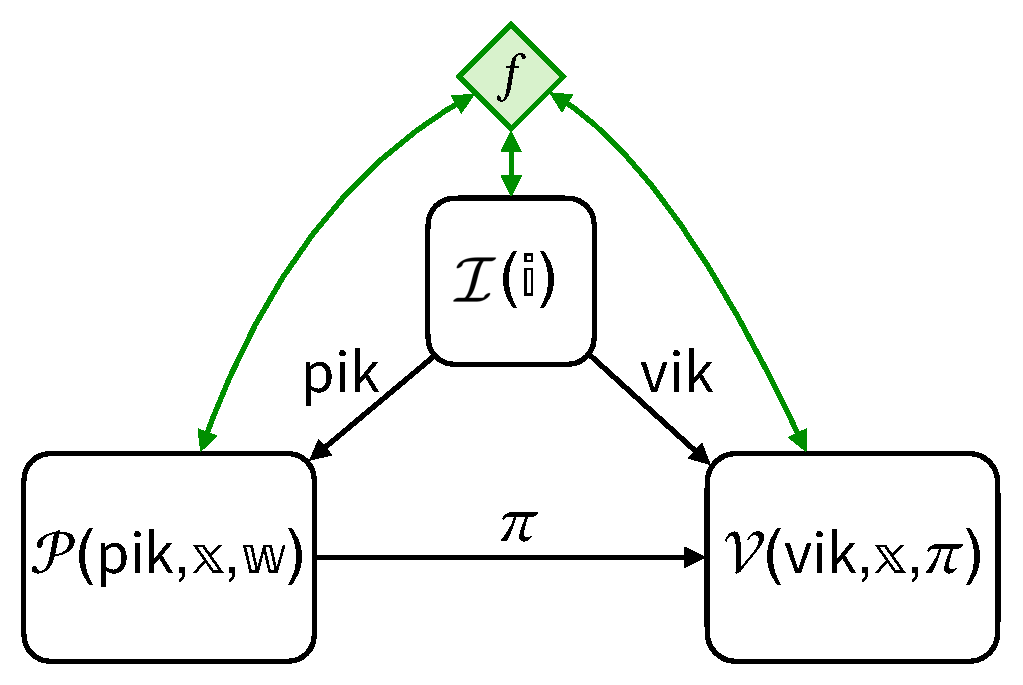
\includegraphics[width=\textwidth]{\FigureFolder/preprocessing-narg-diagram}
  \caption{}
  \label{figure:preprocessing-narg-diagram}
\end{subfigure}
\quad
\begin{subfigure}[b]{0.4\textwidth}
  \centering
  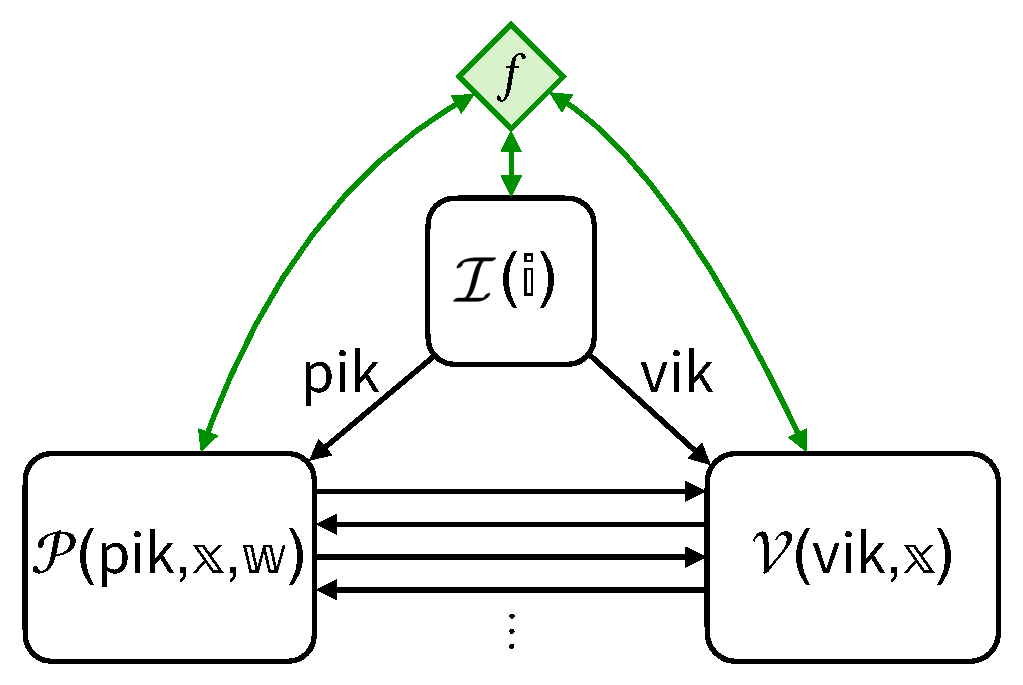
\includegraphics[width=\textwidth]{\FigureFolder/preprocessing-iarg-diagram}
  \caption{}
  \label{figure:preprocessing-iarg-diagram}
\end{subfigure}
\caption[Diagram of a preprocessing NARG and a preprocessing IARG.]{Diagram of a preprocessing non-interactive argument (left) and a preprocessing interactive argument (right), in the random oracle model. }
\label{figure:preprocessing-arg-diagrams}
\end{figure}

%%%%%%%%%%%%%%%%%%%%%%%%%%%%%%%%%%%%%%%%%%%%%%%%%%%%%%%%%%%%%%%%%%%%%%%%%%%%%%%
%%%%%%%%%%%%%%%%%%%%%%%%%%%%%%%%%%%%%%%%%%%%%%%%%%%%%%%%%%%%%%%%%%%%%%%%%%%%%%%
%%%%%%%%%%%%%%%%%%%%%%%%%%%%%%%%%%%%%%%%%%%%%%%%%%%%%%%%%%%%%%%%%%%%%%%%%%%%%%%
\section{The holographic setting}
\label{section:motivate-holography}

In \Cref{section:motivate-preprocessing} we motivated and outlined the preprocessing setting, an offline-online model for argument systems. Here we informally discuss the \textbf{holographic setting}, which is an offline-online model analogously defined for probabilistic proof systems.

Similarly to preprocessing argument systems, holographic probabilistic proofs:
\begin{inparaenum}[(a)]
  \item consider relations and languages that are indexed (see \Cref{definition:indexed-relation-and-language}), and
  \item additionally involve an \emph{indexer algorithm} $\IOPFormat{\ProtoIndexer}$.
\end{inparaenum}
The offline phase and online phase work as follows.
\begin{itemize}
  \item \emph{Offline phase.}
  The indexer $\IOPFormat{\ProtoIndexer}$ is a deterministic algorithm that receives as input an index $\Index$ and outputs two \DoQuote{encoded indices}, a \emph{prover encoded index} $\ProverEncodedIndex$ and a \emph{verifier encoded index} $\VerifierEncodedIndex$. Hence, the offline phase consists of the computation $(\ProverEncodedIndex,\VerifierEncodedIndex) \DefineEqual \IOPFormat{\ProtoIndexer}(\Index)$. Note that the offline phase depends solely on the index $\Index$ and, in particular, the same encoded indices can be used for different instances $\Instance$ and witnesses $\Witness$ (which are unknown until the online phase).
  \item \emph{Online phase.}
Recall that in a (non-holographic) probabilistic proof the prover receives as input an instance $\Instance$ and a witness $\Witness$ and the verifier receives as input the instance $\Instance$. In a holographic probabilistic proof, the prover and verifier additionally receive information from the offline phase: the prover additionally receives as input the prover encoded index $\ProverEncodedIndex$ and the verifier additionally receives \emph{query access} to the verifier encoded index $\VerifierEncodedIndex$. In particular, the verifier encoded index $\VerifierEncodedIndex$ is an oracle intended to enable the verifier to check statements about the index $\Index$ without receiving the index $\Index$ (or $\VerifierEncodedIndex$) as an explicit input. The prover and verifier interact according to whichever type of probabilistic proof one is considering, and the verifier eventually outputs a decision bit.
\end{itemize}
In \Cref{figure:holographic-probabilistic-proofs} we show diagrams for holographic versions of every type of probabilistic proof that we consider in this book (SP, IP, PCP, IOP); the diagrams make evident how each type of probabilistic proof is modified in the same way to obtain the corresponding holographic version.

In \Cref{section:holographic-iop} we provide a formal treatment of holographic IOPs. Definitions for the holographic versions of other probabilistic proofs in this book (SP, IP, PCP) are special cases of the definitions for holographic IOPs. Note that, in all security notions, the verifier encoded index $\VerifierEncodedIndex$ is \DoQuote{trusted} in the sense that the verifier is guaranteed to receive query access to the correct output of the indexer, regardless of what a malicious prover may do.\footnote{This is analogous to how, in a preprocessing argument, the argument verifier receives as input the correct verifier index key, regardless of what a malicious argument prover may do.}

\begin{figure}[htp!]
\centering
\begin{subfigure}[b]{0.4\textwidth}
\centering
  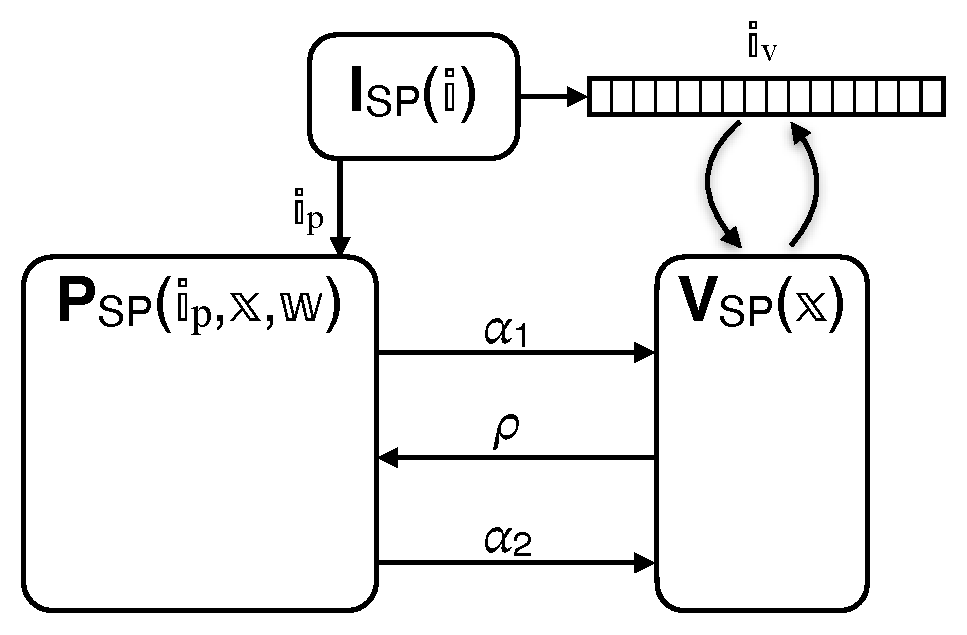
\includegraphics[width=\textwidth]{\FigureFolder/holographic-sp-diagram}
  \caption{}
  \label{figure:holographic-sp-diagram}
\end{subfigure}
\quad
\begin{subfigure}[b]{0.4\textwidth}
  \centering
  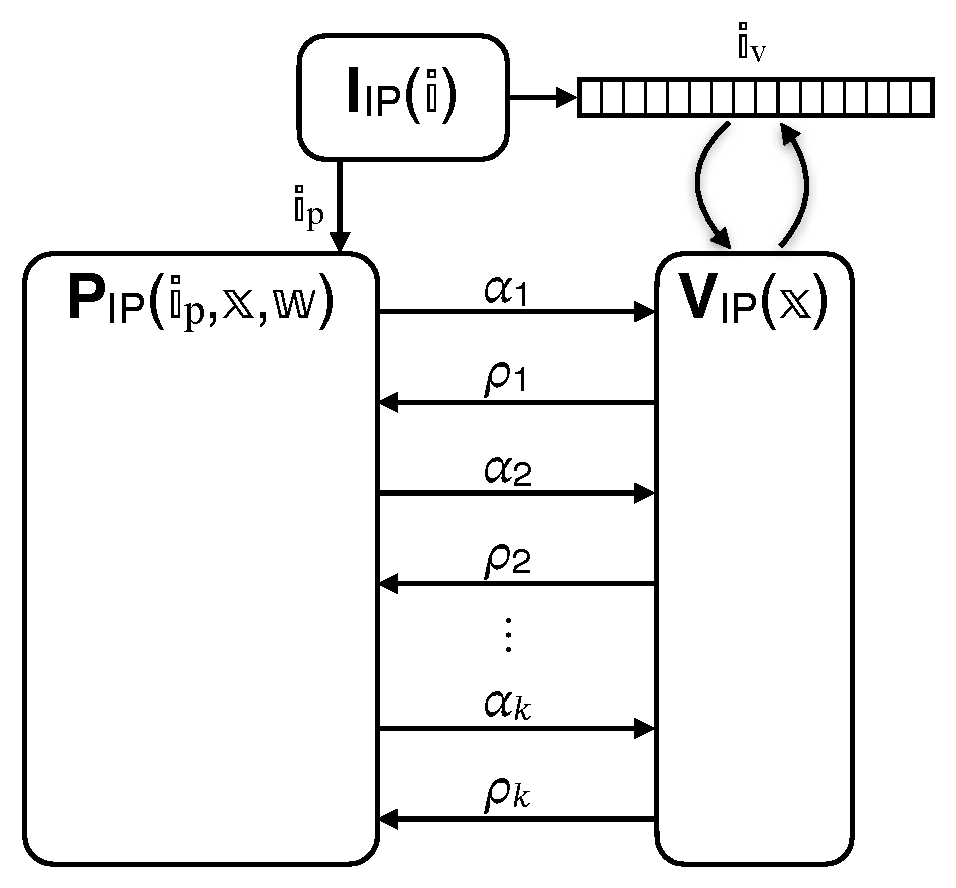
\includegraphics[width=\textwidth]{\FigureFolder/holographic-ip-diagram}
  \caption{}
  \label{figure:holographic-ip-diagram}
\end{subfigure}
\begin{subfigure}[b]{0.4\textwidth}
\centering
  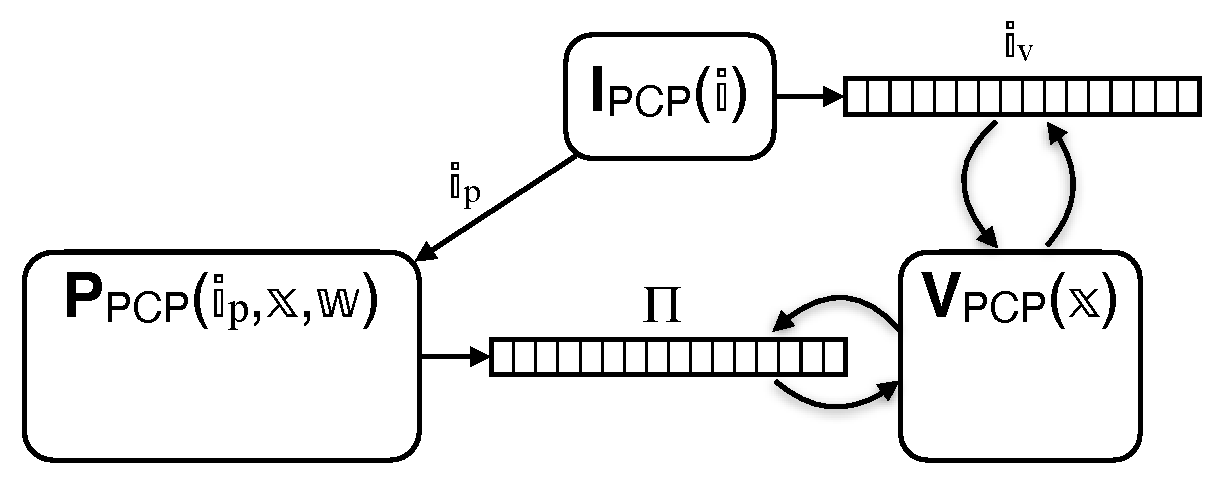
\includegraphics[width=\textwidth]{\FigureFolder/holographic-pcp-diagram}
  \caption{}
  \label{figure:holographic-pcp-diagram}
\end{subfigure}
\quad
\begin{subfigure}[b]{0.4\textwidth}
  \centering
  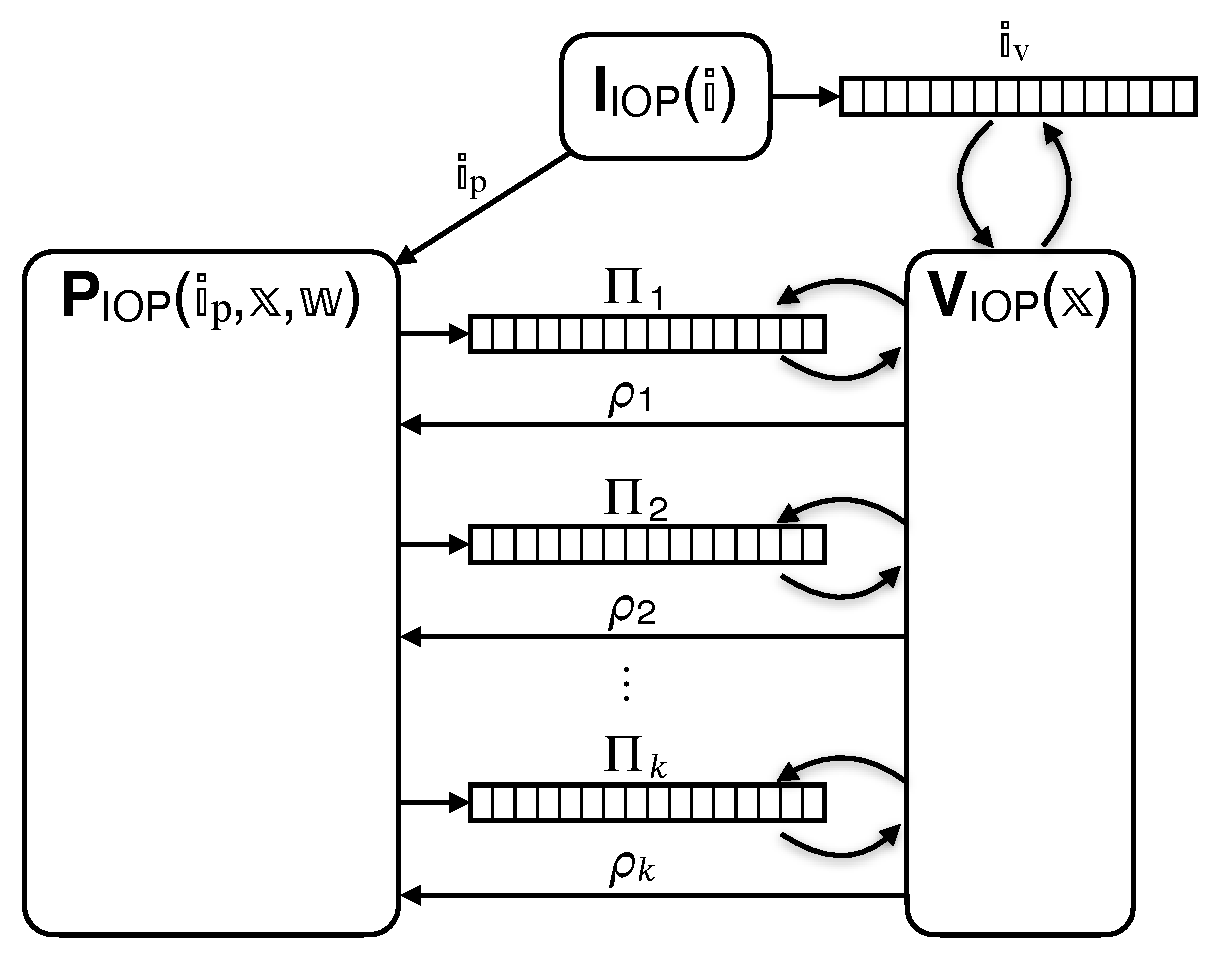
\includegraphics[width=\textwidth]{\FigureFolder/holographic-iop-diagram}
  \caption{}
  \label{figure:holographic-iop-diagram}
\end{subfigure}
\caption[Diagrams of holographic probabilistic proofs.]{Diagram of a holographic SP (top left), holographic IP (top right), holographic PCP (bottom left), and holographic IOP (bottom right).}
\label{figure:holographic-probabilistic-proofs}
\end{figure}

%%%%%%%%%%%%%%%%%%%%%%%%%%%%%%%%%%%%%%%%%%%%%%%%%%%%%%%%%%%%%%%%%%%%%%%%%%%%%%%
%%%%%%%%%%%%%%%%%%%%%%%%%%%%%%%%%%%%%%%%%%%%%%%%%%%%%%%%%%%%%%%%%%%%%%%%%%%%%%%
%%%%%%%%%%%%%%%%%%%%%%%%%%%%%%%%%%%%%%%%%%%%%%%%%%%%%%%%%%%%%%%%%%%%%%%%%%%%%%%
\section{From holography to preprocessing}
\label{section:from-holography-to-preprocessing}

We informally explain how any \emph{holographic} probabilistic proof system naturally leads to a \emph{preprocessing} argument system in the ROM. The idea underlying this implication is intuitive and flexible: every transformation studied in this book can be extended to support holography-to-preprocessing, and similar extensions hold in other settings (e.g., beyond the pure ROM). Later, in \Cref{section:cos-transformation} we provide a detailed description of this idea for the case of preprocessing NARGs constructed from holographic IOPs, which is known as the COS transformation.

\parhead{The argument indexer}
We describe how to construct, in the ROM, an argument indexer $\ARGIndexer$ starting from a given indexer $\PPIndexer$ for an underlying probabilistic proof (SP, IP, PCP, IOP). The argument indexer $\ARGIndexer$, given an index $\Index$ and access to a random oracle (or random oracles), is tasked with producing a prover index key $\ARGpik$ and a verifier index key $\ARGvik$ that can be used, respectively, by the argument prover $\ARGProver$ and argument verifier $\ARGVerifier$ in the online phase later on. First $\ARGIndexer$ runs $\PPIndexer$, obtaining encoded indices $\ProverEncodedIndex$ and $\VerifierEncodedIndex$ for the prover and verifier respectively. The verifier of the probabilistic proof will want to query $\VerifierEncodedIndex$; to facilitate this, $\ARGIndexer$ commits to $\VerifierEncodedIndex$ via the Merkle commitment scheme using a random oracle $\ROIndexTreeFunction$, resulting in a Merkle commitment $\MTCommitment_{\IndexRoundSubscript}$ (to include in $\ARGvik$) and trapdoor $\MTTrapdoor_{\IndexRoundSubscript}$. As no hiding properties are needed, the Merkle commitment scheme is configured without salts (the salt size is set to zero). Moreover, the argument verifier $\ARGVerifier$ may need to hash the \DoQuote{full instance} $(\Index,\Instance)$; to facilitate this, $\ARGIndexer$ uses a random oracle $\ROIndexHashFunction$ to hash the index to obtain $\HashedIndex \DefineEqual \ROIndexHashFunction(\Index)$ to include in $\ARGvik$, so that the argument verifier $\ARGVerifier$ may hash $(\HashedIndex,\Instance)$ instead of $(\Index,\Instance)$. The prover index $\ARGpik$ is set to $(\ProverEncodedIndex,\VerifierEncodedIndex,\MTTrapdoor_{\IndexRoundSubscript},\HashedIndex)$ and the verifier index key $\ARGvik$ is set to $(\MTCommitment_{\IndexRoundSubscript},\HashedIndex)$.

The above strategy is summarized in the construction of the argument indexer below, and essentially remains the same no matter the online phase or probabilistic proof.

\begin{construction}
\label{construction:argument-indexer}
Let $\PPIndexer$ be the indexer of the probabilistic proof, which receives as input an index $\Index$ and outputs a prover encoded index $\ProverEncodedIndex$ and verifier encoded index $\VerifierEncodedIndex$; let alphabet $\ProtoAlphabet_{\IndexRoundSubscript}$ be the alphabet of $\VerifierEncodedIndex$ and $\ProtoProofLength_{\IndexRoundSubscript}$ the length of $\VerifierEncodedIndex$ (over this alphabet). Define $\MTSymbol_{\IndexRoundSubscript} \DefineEqual \MTConstructor{\SecurityParameter}{\ProtoAlphabet_{\IndexRoundSubscript}}{\ProtoProofLength_{\IndexRoundSubscript}}{0}$ to be the Merkle commitment scheme for random oracle output size $\SecurityParameter$, messages over alphabet $\ProtoAlphabet_{\IndexRoundSubscript}$ of length $\ProtoProofLength_{\IndexRoundSubscript}$, and salt size $0$ (no hiding properties). We describe an argument indexer $\ARGIndexer$, which receives as input an index $\Index$ and query access to random oracles $(\ROIndexTreeFunction,\ROIndexHashFunction) \in \RODistribution{(\SecurityParameter,\SecurityParameter)}$, and outputs a prover index key $\ARGpik$ and verifier index key $\ARGvik$.
\begin{itemize}
\item[] $\ARGIndexer^{(\ROIndexTreeFunction,\ROIndexHashFunction)}(\Index)$:
\begin{enumerate}[nolistsep]
  \item Compute a hash of the index: $\HashedIndex \DefineEqual \ROIndexHashFunction(\Index) \in \Bits^{\SecurityParameter}$.\footnote{This step can be omitted in case the argument verifier does not need to hash the full instance $(\Index,\Instance)$, which is the case when constructing preprocessing \emph{interactive} arguments (because, in such a case, the Fiat--Shamir transformation is not used). Specifically, this step can be omitted for the preprocessing extensions of the Kilian transformation and of the iBCS transformation. In this case, $\HashedIndex$ is omitted from $\ARGpik$ and $\ARGvik$. \label{footnote:cos-for-ibcs-simplifies}}
  \item Compute the prover encoded index and verifier encoded index: $(\ProverEncodedIndex,\VerifierEncodedIndex) \DefineEqual \PPIndexer(\Index)$.
  \item Commit to $\VerifierEncodedIndex$ via the Merkle commitment scheme $\MTSymbol_{\IndexRoundSubscript}$:
  \begin{equation*}
  (\MTCommitment_{\IndexRoundSubscript},\MTTrapdoor_{\IndexRoundSubscript}) \DefineEqual \MTIdxCommit{\IndexRoundSubscript}^{\ROIndexTreeFunction}(\VerifierEncodedIndex)
  \enspace.
  \end{equation*}
  \item Set the prover index key $\ARGpik \DefineEqual (\ProverEncodedIndex,\VerifierEncodedIndex,\MTTrapdoor_{\IndexRoundSubscript},\HashedIndex)$
  \item Set the verifier index key $\ARGvik \DefineEqual (\MTCommitment_{\IndexRoundSubscript},\HashedIndex)$.
  \item Output $(\ARGpik,\ARGvik)$.
\end{enumerate}
\end{itemize}
Note that $\ARGIndexer$ is a deterministic algorithm, profiting from the benefits discussed in \Cref{remark:probabilistic-argument-indexer}.
\end{construction}

\parhead{The argument prover and verifier}
The argument prover $\ARGProver$ and argument verifier $\ARGVerifier$ are constructed from the prover $\PPProver$ and verifier $\PPVerifier$ of the probabilistic proof. The construction is similar to the relevant transformation in the non-preprocessing setting except for certain differences.
\begin{itemize}
  \item $\ARGProver$ and $\ARGVerifier$ additionally receive as input $\ARGpik = (\ProverEncodedIndex,\VerifierEncodedIndex,\MTTrapdoor_{\IndexRoundSubscript},\HashedIndex)$ and $\ARGvik = (\MTCommitment_{\IndexRoundSubscript},\HashedIndex)$, respectively.
  \item $\ARGProver$ additionally sends answers $\IOPEntries_{\IndexRoundSubscript}$ to the queries $\IOPQuerySet_{\IndexRoundSubscript}$ of $\PPVerifier$ to the verifier encoded index $\VerifierEncodedIndex$, and a corresponding Merkle opening proof $\MTProof_{\IndexRoundSubscript}$ (computed from the trapdoor $\MTTrapdoor_{\IndexRoundSubscript}$ and query set $\IOPQuerySet_{\IndexRoundSubscript}$) relative to the Merkle commitment $\MTCommitment_{\IndexRoundSubscript}$.
  \item $\ARGVerifier$ answers the queries $\IOPQuerySet_{\IndexRoundSubscript}$ of $\PPVerifier$ to the verifier encoded index by using the answers $\IOPEntries_{\IndexRoundSubscript}$ received from the argument prover, and checks the validity of these query-answer pairs by using the Merkle commitment $\MTCommitment_{\IndexRoundSubscript}$ included in $\ARGvik$ by $\ARGIndexer$ and the Merkle opening proof $\MTProof_{\IndexRoundSubscript}$ received from $\ARGProver$. Moreover, if relevant, $\ARGVerifier$ hashes the (short) pair $(\HashedIndex,\Instance)$ rather than the (long) full instance $(\Index,\Instance)$, which intuitively suffices since $\HashedIndex$ is the hash of $\Index$ included in $\ARGvik$ by $\ARGIndexer$.
\end{itemize}

%%%%%%%%%%%%%%%%%%%%%%%%%%%%%%%%%%%%%%%%%%%%%%%%%%%%%%%%%%%%%%%%%%%%%%%%%%%%%%%
%%%%%%%%%%%%%%%%%%%%%%%%%%%%%%%%%%%%%%%%%%%%%%%%%%%%%%%%%%%%%%%%%%%%%%%%%%%%%%%
%%%%%%%%%%%%%%%%%%%%%%%%%%%%%%%%%%%%%%%%%%%%%%%%%%%%%%%%%%%%%%%%%%%%%%%%%%%%%%%
\section{Non-interactive arguments with preprocessing}
\label{section:preprocessing-narg}

Recall that a NARG in the ROM is a pair of oracle algorithms $\NARGSymbol=\ARGSystem$. In contrast, a \emph{preprocessing} NARG in the ROM is a triple of oracle algorithms
\begin{equation*}
\PNARGSymbol=\PARGSystem
\end{equation*}
where $\ARGIndexer$ is the \emph{argument indexer}, $\ARGProver$ is the \emph{argument prover}, and $\ARGVerifier$ is the \emph{argument verifier}. The algorithm $\ARGIndexer$ is deterministic (in order to reduce the need to trust the offline phase as discussed in \Cref{remark:probabilistic-argument-indexer}) and the algorithms $\ARGProver$ and $\ARGVerifier$ may be probabilistic.

We discussed two settings for NARGs: the single oracle setting in \Cref{chapter:argument-definitions,chapter:narg-advanced} and the multi-oracle setting in \Cref{chapter:multiple-oracles-reduction}. The multi-oracle setting extends the single-oracle setting in that the NARG comes with an \emph{oracle configuration} $\ARGOracles$ that specifies the number and output length of random oracles used by the NARG (see \Cref{definition:narg-oracle-configuration}); this configuration may depend on the security parameter and other things like an instance size bound. For the constructions studied in this book it is more convenient to use the definitions for the multi-oracle setting. Therefore, in this section we provide definitions for preprocessing NARGs in the multi-oracle setting. The single-oracle setting is directly implied, analogously to the case of (non-preprocessing) NARGs discussed in \Cref{chapter:multiple-oracles-reduction}.

A preprocessing NARG (in the multi-oracle setting) with oracle configuration $\ARGOracles$ works as follows. Given an index size bound $\IndexSize$ and an instance size bound $\InstanceSize$, random oracles $\ROFunction$ are sampled from the distribution $\RODistribution{\ARGOracles(\SecurityParameter,\IndexSize,\InstanceSize)}$. Anyone can query the oracles $\ROFunction$, including the argument indexer $\ARGIndexer$, the argument prover $\ARGProver$, and the argument verifier $\ARGVerifier$.
\begin{itemize}
  \item \emph{Offline phase.}
  The argument indexer $\ARGIndexer$ receives as input an index $\Index$, and outputs a prover index key $\ARGpik$ and a verifier index key $\ARGvik$. The keys $\ARGpik$ and $\ARGvik$ can be used to prove and verify any number of statements involving the index $\Index$, with any instance $\Instance$ and witness $\Witness$.
  \item \emph{Online phase.}
  The argument prover $\ARGProver$ receives as input the prover index key $\ARGpik$, an instance $\Instance$, and a witness $\Witness$, and outputs an argument string $\ARGString$. The argument verifier $\ARGVerifier$ receives as input the verifier index key $\ARGvik$, the instance $\Instance$, and the argument string $\ARGString$, and outputs a bit denoting whether to accept (the bit is $1$) or reject (the bit is $0$).
\end{itemize}
See \Cref{figure:preprocessing-narg-diagram} for a diagram of a preprocessing NARG.

\parhead{Basic security definitions}
$\PNARGSymbol=\PARGSystem$ is a preprocessing NARG in the ROM for an indexed relation $\IndexedRelation$ if it satisfies two main properties: \emph{(perfect) completeness} and \emph{soundness}.
\begin{itemize}

  \item \textbf{Completeness.}
  Informally, for every index-instance-witness triple $(\Index,\Instance,\Witness) \in \IndexedRelation$, the argument indexer $\ARGIndexer$ on input $\Index$ outputs a key pair $(\ARGpik,\ARGvik)$ and the (honest) argument prover $\ARGProver$ on input $(\ARGpik,\Instance,\Witness)$ outputs an argument string $\ARGString$ such that the argument verifier $\ARGVerifier$ on input $(\ARGvik,\Instance,\ARGString)$ accepts, with probability $1$. The probability here is taken over the choice of random oracle $\ROFunction$, as well as any randomness of $\ARGIndexer,\ARGProver,\ARGVerifier$.

  \item \textbf{Soundness.}
  Informally, every malicious argument prover $\Malicious{\ARGProver}$ convinces the (honest) argument verifier $\ARGVerifier$ to accept an index-instance pair $(\Index,\Instance) \notin \GetLanguage{\IndexedRelation}$ with at most a small error probability that we denote by $\ARGSoundnessError$ (the probability is over the choice of random oracle $\ROFunction$, as well as any randomness of $\Malicious{\ARGProver},\ARGVerifier$); the argument verifier $\ARGVerifier$ receives the verifier index key $\ARGvik$ output by the argument indexer $\ARGIndexer$ rather than the index $\Index$ itself.

The malicious argument prover $\Malicious{\ARGProver}$ is computationally unbounded but may make at most $\ROQueryBound$ queries to the random oracle, for a given query bound $\ROQueryBound \in \Naturals$. In general, the error probability $\ARGSoundnessError$ depends on the query bound $\ROQueryBound$, in addition to the security parameter $\SecurityParameter$. We consider the \emph{adaptive} variant of soundness, capturing the case where the malicious argument prover $\Malicious{\ARGProver}$ chooses the index $\Index$ and instance $\Instance$ adaptively after interacting with the random oracle. Hence $\ARGSoundnessError$ also depends on an index size bound $\IndexSize$ and an instance size bound $\InstanceSize$.

\end{itemize}
Below we provide the definitions of (perfect) completeness and (adaptive) soundness.


\begin{definition}
\label{definition:preprocessing-narg-completeness-with-cnf}
A preprocessing non-interactive argument $\PNARGSymbol=\PARGSystem$ for an indexed relation $\IndexedRelation$ with oracle configuration $\ARGOracles$ has \defemph{(perfect) completeness} if for every security parameter $\SecurityParameter \in \Naturals$, index size bound $\IndexSize \in \Naturals$, instance size bound $\InstanceSize \in \Naturals$, and index-instance-witness triple $(\Index,\Instance,\Witness) \in \IndexedRelation$ with $\SomeSize{\Index} \leq \IndexSize$ and $\SomeSize{\Instance} \leq \InstanceSize$,
\begin{equation*}
\Pr\left[
  \ARGVerifier^{\ROFunction}(\ARGvik,\Instance,\ARGString)=1
\GivenExperiment
\StateExperiment{
  \ROFunction \gets \RODistribution{\ARGOracles(\SecurityParameter,\IndexSize,\InstanceSize)} \\
  (\ARGpik,\ARGvik) \DefineEqual \ARGIndexer^{\ROFunction}(\Index) \\
  \ARGString \gets \ARGProver^{\ROFunction}(\ARGpik,\Instance,\Witness)
}
\right] = 1
\enspace.
\end{equation*}
The probability is taken over $\ROFunction$ and any randomness of $\ARGProver,\ARGVerifier$.
\end{definition}

\begin{definition}
\label{definition:preprocessing-narg-adaptive-soundness-with-cnf}
A preprocessing non-interactive argument $\PNARGSymbol=\PARGSystem$ for an indexed relation $\IndexedRelation$ with oracle configuration $\ARGOracles$ has \defemph{adaptive soundness error} $\ARGSoundnessError$ if for every security parameter $\SecurityParameter \in \Naturals$, query bound $\ROQueryBound \in \Naturals$, $\ROQueryBound$-query malicious argument prover $\Malicious{\ARGProver}$, index size bound $\IndexSize \in \Naturals$, and instance size bound $\InstanceSize \in \Naturals$,
\begin{equation*}
\Pr\left[
\begin{array}{l}
  \SomeSize{\Index} \leq \IndexSize \\
  \land\;\SomeSize{\Instance} \leq \InstanceSize \\
  \land\;(\Index,\Instance) \notin \GetLanguage{\IndexedRelation} \\
  \land\;\ARGVerifier^{\ROFunction}(\ARGvik,\Instance,\ARGString)=1
\end{array}
\GivenExperiment
\StateExperiment{
  \ROFunction \gets \RODistribution{\ARGOracles(\SecurityParameter,\IndexSize,\InstanceSize)} \\
  (\Index,\AuxiliaryState) \gets \Malicious{\ARGProver}^{\ROFunction} \\
  (\ARGpik,\ARGvik) \DefineEqual \ARGIndexer^{\ROFunction}(\Index) \\
  (\Instance,\ARGString) \gets \Malicious{\ARGProver}^{\ROFunction}(\AuxiliaryState,\ARGpik,\ARGvik)
}
\right]
\leq
\ARGSoundnessError(\SecurityParameter,\ROQueryBound,\IndexSize,\InstanceSize)
\enspace.
\end{equation*}
The probability is taken over $\ROFunction$ and any randomness of $\Malicious{\ARGProver},\ARGVerifier$.
\end{definition}

\parhead{Additional security definitions}
In \Cref{chapter:narg-advanced} we additionally consider \emph{knowledge soundness} (both straightline and rewinding) and \emph{zero knowledge} for NARGs in the ROM. Below we provide analogous definitions for preprocessing NARGs in the ROM:
\begin{itemize}[noitemsep]
  \item \Cref{definition:preprocessing-adaptive-straightline-knowledge-soundness-with-cnf} is straightline knolwedge soundness;
  \item \Cref{definition:preprocessing-adaptive-rewinding-knowledge-soundness-with-cnf} is rewinding knowledge soundness (and \Cref{definition:preprocessing-argument-failure-probability-with-cnf} is failure probability);
  \item \Cref{definition:preprocessing-narg-adaptive-zk-with-cnf} is adaptive zero knowledge.
\end{itemize}

\begin{definition}
\label{definition:preprocessing-adaptive-straightline-knowledge-soundness-with-cnf}
A preprocessing non-interactive argument $\PNARGSymbol=\PARGSystem$ for an indexed relation $\IndexedRelation$ with oracle configuration $\ARGOracles$ has \defemph{straightline knowledge soundness error $\ARGKnowledgeError$} if there exists a polynomial-time deterministic algorithm $\ARGExtractor$ (the \emph{extractor}) such that for every security parameter $\SecurityParameter \in \Naturals$, query bound $\ROQueryBound \in \Naturals$, $\ROQueryBound$-query deterministic argument prover $\Malicious{\ARGProver}$, index size bound $\IndexSize \in \Naturals$, and instance size bound $\InstanceSize \in \Naturals$,
\begin{equation*}
\Pr\left[
\begin{array}{l}
  \SomeSize{\Index} \leq \IndexSize \\
  \land\;\SomeSize{\Instance} \leq \InstanceSize \\
  \land\;(\Index,\Instance,\Witness) \notin \IndexedRelation \\
  \land\;\ARGVerifier^{\ROFunction}(\ARGvik,\Instance,\ARGString)=1
\end{array}
\GivenExperiment
\StateExperiment{
  \ROFunction \gets \RODistribution{\ARGOracles(\SecurityParameter,\IndexSize,\InstanceSize)} \\
  \ROOutputAndTrace{\ROFunction}{\Malicious{\ARGProver}}{\ROTrace_{1}}{(\Index,\AuxiliaryState)} \\
  (\ARGpik,\ARGvik) \xleftarrow{\ROTraceIndexer} \ARGIndexer^{\ROFunction}(\Index) \\
  \ROInputOutputAndTrace{\ROFunction}{\Malicious{\ARGProver}}{\AuxiliaryState,\ARGpik,\ARGvik}{\ROTrace_{2}}{(\Instance,\ARGString)} \\
  \Witness \gets \ARGExtractor(\Index,\Instance,\ARGString,\ROTrace_{1},\ROTraceIndexer,\ROTrace_{2})
}
\right]
\leq
\ARGKnowledgeError(\SecurityParameter,\ROQueryBound,\IndexSize,\InstanceSize)
\enspace.
\end{equation*}
\end{definition}

\begin{definition}
\label{definition:preprocessing-argument-failure-probability-with-cnf}
Let $\PNARGSymbol=\PARGSystem$ be a preprocessing non-interactive argument. A deterministic argument prover $\Malicious{\ARGProver}$ has \defemph{failure probability $\ProverFailureProbability{\Malicious{\ARGProver}}$} if for every security parameter $\SecurityParameter \in \Naturals$, index size bound $\IndexSize \in \Naturals$, and instance size bound $\InstanceSize \in \Naturals$,
\begin{equation*}
\Pr\left[
\begin{array}{l}
  \SomeSize{\Index} > \IndexSize \\
  \lor\;\SomeSize{\Instance} > \InstanceSize \\
  \lor\;\ARGVerifier^{\ROFunction}(\ARGvik,\Instance,\ARGString)=0
\end{array}
\GivenExperiment
\StateExperiment{
  \ROFunction \gets \RODistribution{\ARGOracles(\SecurityParameter,\IndexSize,\InstanceSize)} \\
  (\Index,\AuxiliaryState) \gets \Malicious{\ARGProver}^{\ROFunction} \\
  (\ARGpik,\ARGvik) \DefineEqual \ARGIndexer^{\ROFunction}(\Index) \\
  (\Instance,\ARGString) \gets \Malicious{\ARGProver}^{\ROFunction}(\AuxiliaryState,\ARGpik,\ARGvik)
}
\right]
\leq
\ProverFailureProbability{\Malicious{\ARGProver}}(\SecurityParameter,\IndexSize,\InstanceSize)
\enspace.
\end{equation*}
\end{definition}

\begin{definition}
\label{definition:preprocessing-adaptive-rewinding-knowledge-soundness-with-cnf}
A preprocessing non-interactive argument $\PNARGSymbol=\PARGSystem$ for an indexed relation $\IndexedRelation$ with oracle configuration $\ARGOracles$ has \defemph{rewinding knowledge soundness error $\ARGKnowledgeError$ with extraction time $\ARGKnowledgeTime$} if there exists a probabilistic algorithm $\ARGExtractor$ (the \emph{extractor}) such that for every security parameter $\SecurityParameter \in \Naturals$, query bound $\ROQueryBound \in \Naturals$, $\ROQueryBound$-query deterministic argument prover $\Malicious{\ARGProver}$ with failure probability $\ProverFailureProbability{\Malicious{\ARGProver}}$ and running time $\ProverRunningTime{\Malicious{\ARGProver}}$, index size bound $\IndexSize \in \Naturals$, and instance size bound $\InstanceSize \in \Naturals$,
\begin{align*}
&\Pr\left[
\begin{array}{l}
  \SomeSize{\Index} \leq \IndexSize \\
  \land\;\SomeSize{\Instance} \leq \InstanceSize \\
  \land\;(\Index,\Instance,\Witness) \notin \IndexedRelation \\
  \land\;\DecisionBit=1
\end{array}
\GivenExperiment
\StateExperiment{
  \ROFunction \gets \RODistribution{\ARGOracles(\SecurityParameter,\IndexSize,\InstanceSize)} \\
  \ROOutputAndTrace{\ROFunction}{\Malicious{\ARGProver}}{\ROTrace_{1}}{(\Index,\AuxiliaryState)} \\
  (\ARGpik,\ARGvik) \xleftarrow{\ROTraceIndexer} \ARGIndexer^{\ROFunction}(\Index) \\
  \ROInputOutputAndTrace{\ROFunction}{\Malicious{\ARGProver}}{\AuxiliaryState,\ARGpik,\ARGvik}{\ROTrace_{2}}{(\Instance,\ARGString)} \\
  \DecisionBit \xleftarrow{\ROTraceVerifier} \ARGVerifier^{\ROFunction}(\ARGvik,\Instance,\ARGString) \\
  \Witness \gets \ARGExtractor(\Index,\ARGpik,\ARGvik,\Instance,\ARGString,\ROTrace_{1},\ROTraceIndexer,\ROTrace_{2},\ROTraceVerifier,\BlackBox{\Malicious{\ARGProver}})
}
\right]
\\ &
\leq
\ARGKnowledgeError\left(\SecurityParameter,\ROQueryBound,\IndexSize,\InstanceSize,\ProverFailureProbability{\Malicious{\ARGProver}}(\SecurityParameter,\IndexSize,\InstanceSize)\right)
\enspace.
\end{align*}
Moreover, $\ARGExtractor$ runs in expected time $\ARGKnowledgeTime\left(\SecurityParameter,\ROQueryBound,\IndexSize,\InstanceSize,\ProverFailureProbability{\Malicious{\ARGProver}}(\SecurityParameter,\IndexSize,\InstanceSize),\ProverRunningTime{\Malicious{\ARGProver}}(\SecurityParameter,\IndexSize,\InstanceSize)\right)$ (over the given inputs and internal randomness).
\end{definition}

\begin{remark}
\Cref{claim:narg-knowledge-soundness-equivalent-definitions} proves the equivalence of two variants of rewinding knowledge soundness for (non-preprocessing) NARGs, \Cref{definition:adaptive-rewinding-knowledge-soundness} and \Cref{definition:adaptive-rewinding-knowledge-soundness-verifier-trace}. A similar equivalence holds for preprocessing NARGs, and \Cref{definition:preprocessing-adaptive-rewinding-knowledge-soundness-with-cnf} is the definition analogous to \Cref{definition:adaptive-rewinding-knowledge-soundness-verifier-trace} where the knowledge extractor receives the query-answer trace of the argument verifier and has no access to the random oracle. We use this definition when proving statements.
\end{remark}

\begin{definition}
\label{definition:preprocessing-narg-adaptive-zk-with-cnf}
A preprocessing non-interactive argument $\PNARGSymbol=\PARGSystem$ for an indexed relation $\IndexedRelation$ with oracle configuration $\ARGOracles$ has \defemph{adaptive zero-knowledge error $\ARGOAZKError$} (in the EPROM) if there exists a probabilistic polynomial-time simulator $\ARGSimulator$ such that, for every security parameter $\SecurityParameter \in \Naturals$, query bound $\ROQueryBound \in \Naturals$, $\ROQueryBound$-query admissible adversary $\ARGAdversary$, index size bound $\IndexSize \in \Naturals$, and instance bound $\InstanceSize \in \Naturals$, the following two distributions are $\ARGOAZKError(\SecurityParameter,\ROQueryBound,\IndexSize,\InstanceSize)$-close in statistical distance:
\begin{equation*}
\Distribution_{\RealSymbol}
\DefineEqual
\left\{
  \ARGOutput
\GivenExperiment
\StateExperiment{
  \ROFunction \gets \RODistribution{\ARGOracles(\SecurityParameter,\IndexSize,\InstanceSize)} \\
  (\Index,\ROAdvState) \gets \ARGAdversary^{\ROFunction} \\
  (\ARGpik,\ARGvik) \DefineEqual \ARGIndexer^{\ROFunction}(\Index) \\
  (\Instance,\Witness,\ROAdvState) \gets \ARGAdversary^{\ROFunction}(\ROAdvState,\ARGpik,\ARGvik) \\
  \ARGString \gets \ARGProver^{\ROFunction}(\ARGpik,\Instance,\Witness) \\
  \ARGOutput \gets \ARGAdversary^{\ROFunction}(\ROAdvState,\ARGString)
}
\right\}
\end{equation*}
and
\begin{equation*}
\Distribution_{\SimSymbol}
\DefineEqual
\left\{
  \ARGOutput
\GivenExperiment
\StateExperiment{
  \ROFunction \gets \RODistribution{\ARGOracles(\SecurityParameter,\IndexSize,\InstanceSize)} \\
  (\Index,\ROAdvState) \gets \ARGAdversary^{\ROFunction} \\
  (\ARGpik,\ARGvik) \DefineEqual \ARGIndexer^{\ROFunction}(\Index) \\
  (\Instance,\Witness,\ROAdvState) \gets \ARGAdversary^{\ROFunction}(\ROAdvState,\ARGpik,\ARGvik) \\
  (\ARGString,\ARGZKProgrammedList) \gets \ARGSimulator^{\ROFunction}(\Index,\Instance) \\
  \ARGOutput \gets \ARGAdversary^{\ROProgram{\ROFunction}{\ARGZKProgrammedList}}(\ROAdvState,\ARGString)
}
\right\}
\enspace.
\end{equation*}
Above, $\ARGAdversary$ is admissible if it always outputs $\Index,\Instance,\Witness$ such that $(\Index,\Instance,\Witness) \in \IndexedRelation$, $\SomeSize{\Index} \leq \IndexSize$, and $\SomeSize{\Instance} \leq \InstanceSize$.
\end{definition}

\begin{remark}[deterministic vs.\ probabilistic argument indexers]
\label{remark:probabilistic-argument-indexer}
The definition of a preprocessing NARG that we consider requires the argument indexer $\ARGIndexer$ to be a \emph{deterministic} algorithm. This is the case in many constructions of interest, including the construction that we study in this chapter. Moreover, $\ARGIndexer$ being deterministic reduces the need for trust in the preprocessing step: anyone can check that a given key pair $(\ARGpik,\ARGvik)$ is the valid output of $\ARGIndexer^{\ROFunction}(\Index)$, because they can rerun the computation and determine if the output matches the key pair.

The more general case of a probabilistic argument indexer $\ARGIndexer$ is meaningful, but may demand placing more trust in the preprocessing step. One option is to require $\ARGIndexer$ to be public-coin, which means that all security properties of a preprocessing NARG hold even if the adversary knows $\ARGIndexer$'s randomness; in this case, $\ARGIndexer$'s randomness can be published and, as in the deterministic case, anyone can use that randomness to determine if a given key pair is the correct output. However, if $\ARGIndexer$ is private-coin (its randomness must remain private) then the offline preprocessing step must be carried out by a trusted party (or cryptographic replacements such as a secure multi-party ceremony), which is undesirable.
\end{remark}

\begin{remark}[delegating the indexer computation]
\label{remark:delegating-the-indexer}
The argument indexer $\ARGIndexer$ performs a deterministic computation to produce the index keys: $(\ARGpik,\ARGvik) \DefineEqual \ARGIndexer^{\ROFunction}(\Index)$. This computation could itself be delegated to an untrusted argument prover in order to reduce the cost of the trusted offline computation, for example, from $\poly(\BitSize{\Index})$ to $O(\BitSize{\Index})$. In this case, the untrusted argument prover would compute the index keys $(\ARGpik,\ARGvik)$ and then prove the statement \DoQuote{$(\ARGpik,\ARGvik) = \ARGIndexer^{\ROFunction}(\Index)$}, resulting in an argument string $\ARGString_{\Index}$ attesting to this statement. The security properties of the preprocessing argument would then hold provided the tuple $(\Index,\ARGpik,\ARGvik,\ARGString_{\Index})$ satisfies the verification procedure of the delegation protocol (which should be cheaper than the computation $\ARGIndexer^{\ROFunction}(\Index)$). This notion of a preprocessing argument naturally arises, e.g., from holographic IOPs wherein there is a public-coin IOP to verify the statement \DoQuote{$(\ProverEncodedIndex,\VerifierEncodedIndex) \DefineEqual \HIOPIndexer(\Index)$}. We limit this remark to point the way to this relaxation without working out the details.
\end{remark}



%%%%%%%%%%%%%%%%%%%%%%%%%%%%%%%%%%%%%%%%%%%%%%%%%%%%%%%%%%%%%%%%%%%%%%%%%%%%%%%
%%%%%%%%%%%%%%%%%%%%%%%%%%%%%%%%%%%%%%%%%%%%%%%%%%%%%%%%%%%%%%%%%%%%%%%%%%%%%%%
%%%%%%%%%%%%%%%%%%%%%%%%%%%%%%%%%%%%%%%%%%%%%%%%%%%%%%%%%%%%%%%%%%%%%%%%%%%%%%%
\section{Holographic IOPs}
\label{section:holographic-iop}

Recall from \Cref{section:iop-definition} that an IOP is a pair of interactive algorithms $\IOPSymbol=\IOPSystem$. In contrast, a \emph{holographic} IOP is a triple of algorithms
\begin{equation*}
\HIOPSymbol=\HIOPSystem
\end{equation*}
that works as follows. The IOP indexer receives as input an index $\Index$ and outputs a prover encoded index $\ProverEncodedIndex$ for the IOP prover and a verifier encoded index $\VerifierEncodedIndex$ for the IOP verifier. The IOP prover $\HIOPProver$ receives as input the prover encoded index $\ProverEncodedIndex$, instance $\Instance$, and a witness $\Witness$, and the IOP verifier $\HIOPVerifier$ receives query access to the verifier encoded index $\VerifierEncodedIndex$ and receives as input the instance $\Instance$. They interact over some number $\IOPRoundComplexity$ of rounds, where in each round $\RoundIndex \in [\IOPRoundComplexity]$ the IOP prover $\HIOPProver$ sends a proof string $\IOPString_{\RoundIndex}$ and then the IOP verifier $\HIOPVerifier$ sends a message $\IOPVerifierMessage_{\RoundIndex}$. The IOP verifier may query any of the received proof strings at any location. After the interaction, the IOP verifier $\HIOPVerifier$ outputs a bit denoting whether to accept or reject, computed based on the instance $\Instance$, the IOP verifier's own randomness, and the answers to any queries to the verifier encoded index $\VerifierEncodedIndex$ and to the proof strings $\IOPStrings$ (these form the entire view of the IOP verifier). The IOP prover and the IOP verifier may be probabilistic, while the IOP indexer is required to be deterministic (see \Cref{remark:probabilistic-iop-indexer}). See \Cref{figure:holographic-iop-diagram} for a diagram of a holographic IOP.

The tuple $\HIOPSymbol=\HIOPSystem$ is an IOP for an indexed relation $\IndexedRelation$ with \emph{(perfect) completeness} and \emph{soundness error $\HIOPSoundnessError$} if it satisfies the two properties stated below.

\begin{definition}
\label{definition:hiop-completeness}
$\HIOPSymbol=\HIOPSystem$ for an indexed relation $\IndexedRelation$ has \defemph{perfect completeness} if for every $(\Index,\Instance,\Witness) \in \IndexedRelation$,
\begin{equation*}
\Pr\left[
\HIOPInteract{\HIOPProver(\ProverEncodedIndex,\Instance,\Witness)}{\HIOPVerifier^{\VerifierEncodedIndex}(\Instance)}=1
\GivenExperiment
\StateExperiment{
(\ProverEncodedIndex,\VerifierEncodedIndex) \DefineEqual \HIOPIndexer(\Index)
}
\right]
=1
\enspace.
\end{equation*}
\end{definition}

\begin{definition}
\label{definition:hiop-soundness}
$\HIOPSymbol=\HIOPSystem$ for an indexed relation $\IndexedRelation$ has \defemph{soundness error $\HIOPSoundnessError$} if for every $(\Index,\Instance) \notin \GetLanguage{\IndexedRelation}$ and malicious IOP prover $\HIOPMaliciousProver$,
\begin{equation*}
\Pr\left[
\HIOPInteract{\HIOPMaliciousProver}{\HIOPVerifier^{\VerifierEncodedIndex}(\Instance)}=1
\GivenExperiment
\StateExperiment{
(\ProverEncodedIndex,\VerifierEncodedIndex) \DefineEqual \HIOPIndexer(\Index)
}
\right]
\leq
\HIOPSoundnessError(\Index,\Instance)
\enspace.
\end{equation*}
We additionally define
\begin{equation*}
\HIOPSoundnessError(\IndexSize,\InstanceSize) \DefineEqual \MaxIndexedSoundness{\HIOPSoundnessError(\Index,\Instance)}
\enspace.
\end{equation*}
\end{definition}

\parhead{Public-coin}
We only consider holographic IOPs that are \emph{public-coin}, analogously to \Cref{definition:iop-public-coin}.

\begin{definition}
\label{definition:hiop-public-coin}
$\HIOPSymbol=\HIOPSystem$ is \defemph{public-coin} if every message $\IOPVerifierRandomMessage_{\RoundIndex}$ sent by the IOP verifier $\HIOPVerifier$ is a random binary string of some prescribed size $\IOPRandomnessComplexity_{\RoundIndex}$ (that is statistically independent of everything else); moreover, the IOP verifier $\HIOPVerifier$ has no other randomness. In this case, the decision bit of the IOP verifier $\HIOPVerifier$ is a function only of the instance $\Instance$, the IOP verifier randomness $\IOPVerifierRandomMessage = \IOPVerifierRandomMessages$, and answers to queries to the verifier encoded index $\VerifierEncodedIndex$ and the received IOP strings $\IOPStrings$. We denote this bit by
\begin{equation*}
\HIOPVerifier^{\VerifierEncodedIndex,\IOPStrings}(\IOPVerifierInput)
\enspace.
\end{equation*}
\end{definition}

\parhead{Efficiency measures}
We are interested in several efficiency measures of a holographic IOP.
\begin{itemize}

  \item \emph{Round complexity}, denoted $\IOPRoundComplexity$, is the number of back-and-forth interactions between the IOP prover and IOP verifier. This excludes the IOP indexer in the offline phase.

  \item \emph{Alphabet}, denoted $\IOPAlphabet$, is the alphabet used to write the verifier encoded index $\VerifierEncodedIndex$ and to write the proof strings $\IOPStrings$. (In general, each of these strings may be over a different alphabet, or multiple alphabets, but for simplicity we focus on one alphabet for all of these strings.)

  \item \emph{Proof length}, denoted $\IOPProofLength$, is the number of symbols across the verifier encoded index $\VerifierEncodedIndex$ and all proof strings $\IOPStrings$. The total number of bits across the verifier encoded index and all proof strings is thus $\IOPProofLength \cdot \log \Cardinality{\IOPAlphabet}$. We denote by $\IOPProofLength_{\IndexRoundSubscript}$ the number of symbols in the verifier encoded index $\VerifierEncodedIndex$ and, for every $\RoundIndex \in [\IOPRoundComplexity]$, we denote by $\IOPProofLength_{\RoundIndex}$ the number of symbols in the proof string $\IOPString_{\RoundIndex}$ in round $\RoundIndex$. Hence $\IOPProofLength =\IOPProofLength_{\IndexRoundSubscript} + \sum_{\RoundIndex \in [\IOPRoundComplexity]} \IOPProofLength_{\RoundIndex}$.

  \item \emph{Randomness complexity}, denoted $\IOPRandomnessComplexity$, is the number of random bits used by the IOP verifier across all rounds. For every $\RoundIndex \in [\IOPRoundComplexity]$, we denote by $\IOPRandomnessComplexity_{\RoundIndex}$ the randomness complexity in round $\RoundIndex$. Hence $\IOPRandomnessComplexity = \sum_{\RoundIndex \in [\IOPRoundComplexity]} \IOPRandomnessComplexity_{\RoundIndex}$.

  \item \emph{Query complexity}, denoted $\IOPQueryComplexity$, is the number of locations in the verifier encoded index $\VerifierEncodedIndex$ and all proof strings $\IOPStrings$ read by the IOP verifier. (Hence each query returns a symbol of $\log \Cardinality{\IOPAlphabet}$ bits.) We denote by $\IOPQueryComplexity_{\IndexRoundSubscript}$ the query complexity to the verifier encoded index $\VerifierEncodedIndex$ and, for every $\RoundIndex \in [\IOPRoundComplexity]$, we denote by $\IOPQueryComplexity_{\RoundIndex}$ the query complexity to the proof string $\IOPString_{\RoundIndex}$ in round $\RoundIndex$. Hence $\IOPQueryComplexity = \IOPQueryComplexity_{\IndexRoundSubscript} + \sum_{\RoundIndex \in [\IOPRoundComplexity]} \IOPQueryComplexity_{\RoundIndex}$.

  \item \emph{Indexer time, prover time, and verifier time}, denoted $\HIOPIndexerTime,\IOPProverTime,\IOPVerifierTime$, are the time complexities of the IOP indexer, of the IOP prover (to output the IOP strings), and of the IOP verifier (to output its decision bit).

\end{itemize}
The above efficiency measures may be functions of the index $\Index$ and instance $\Instance$ (and possibly other parameters associated to the construction of an IOP).

\parhead{Knowledge soundness}
We provide definitions for rewinding and straightline knowledge soundness for holographic IOPs, that are analogous to those of (non-holographic) IOPs.

\begin{definition}
\label{definition:hiop-failure-probability}
Let $\HIOPSymbol=\HIOPSystem$ be a holographic IOP. A deterministic IOP prover $\HIOPMaliciousProver$ has \defemph{failure probability $\ProverFailureProbability{\HIOPMaliciousProver}$} if for every index $\Index$ and instance $\Instance$,
\begin{equation*}
\Pr\left[
\HIOPInteract{\HIOPMaliciousProver}{\IOPVerifier^{\VerifierEncodedIndex}(\Instance)}=0
\GivenExperiment
\StateExperiment{
(\ProverEncodedIndex,\VerifierEncodedIndex) \DefineEqual \HIOPIndexer(\Index)
}
\right]
\leq \ProverFailureProbability{\HIOPMaliciousProver}(\Index,\Instance)
\enspace.
\end{equation*}
\end{definition}

\begin{definition}
\label{definition:hiop-knowledge-soundness}
$\HIOPSymbol=\HIOPSystem$ for an indexed relation $\IndexedRelation$ has \defemph{rewinding knowledge soundness error $\HIOPKnowledgeError$ with extraction time $\HIOPKnowledgeTime$} if there exists a probabilistic algorithm $\HIOPExtractor$ (the \emph{extractor}) such that for every index $\Index$, instance $\Instance$, and deterministic IOP prover $\HIOPMaliciousProver$ with running time $\ProverRunningTime{\HIOPMaliciousProver}$, the following holds:
\begin{equation*}
\Pr\left[
\begin{array}{l}
(\Index,\Instance,\Witness) \notin \IndexedRelation \\
\land\;\DecisionBit=1
\end{array}
\GivenExperiment
\StateExperiment{
(\ProverEncodedIndex,\VerifierEncodedIndex) \DefineEqual \HIOPIndexer(\Index) \\
\DecisionBit \xleftarrow{\IOPTranscript} \HIOPInteract{\HIOPMaliciousProver}{\HIOPVerifier^{\VerifierEncodedIndex}(\Instance)} \\
\Witness \gets \HIOPExtractor(\Index,\Instance,\IOPTuple{\IOPString},\IOPTuple{\IOPVerifierRandomMessage},\BlackBox{\HIOPMaliciousProver})
}
\right]
\leq
\HIOPKnowledgeError(\Index,\Instance,\ProverFailureProbability{\HIOPMaliciousProver}(\Index,\Instance))
\enspace.
\end{equation*}
Moreover, $\HIOPExtractor(\Index,\Instance,\IOPTuple{\IOPString},\IOPTuple{\IOPVerifierRandomMessage},\BlackBox{\HIOPMaliciousProver})$ runs in expected time
\begin{equation*}
\HIOPKnowledgeTime(\Index,\Instance,\ProverFailureProbability{\HIOPMaliciousProver}(\Index,\Instance),\ProverRunningTime{\HIOPMaliciousProver}(\Index,\Instance))
\enspace.
\end{equation*}
We additionally define
\begin{align*}
\HIOPKnowledgeError(\IndexSize,\InstanceSize,\ProverFailureProbability{\HIOPMaliciousProver}) &\DefineEqual \MaxIndexedKnowledge{\HIOPKnowledgeError(\Index,\Instance,\ProverFailureProbability{\HIOPMaliciousProver}(\Index,\Instance))}
\enspace,\quad\text{and} \\
\HIOPKnowledgeTime(\IndexSize,\InstanceSize,\ProverFailureProbability{\HIOPMaliciousProver},\ProverRunningTime{\HIOPMaliciousProver}) &\DefineEqual \MaxIndexedKnowledge{\HIOPKnowledgeTime(\Index,\Instance,\ProverFailureProbability{\HIOPMaliciousProver}(\Index,\Instance),\ProverRunningTime{\HIOPMaliciousProver}(\Index,\Instance))}
\enspace.
\end{align*}
\end{definition}

\begin{definition}
\label{definition:hiop-knowledge-straightline}
$\HIOPSymbol=\HIOPSystem$ for an indexed relation $\IndexedRelation$ has \defemph{straightline knowledge soundness error $\HIOPKnowledgeError$} if there exists a polynomial-time deterministic algorithm $\HIOPExtractor$ (the \emph{extractor}) such that for every deterministic IOP prover $\HIOPMaliciousProver$, index $\Index$, and instance $\Instance$,
\begin{equation*}
\Pr\left[
\begin{array}{l}
(\Index,\Instance,\Witness) \notin \IndexedRelation \\
\land\;\DecisionBit=1
\end{array}
\GivenExperiment
\StateExperiment{
(\ProverEncodedIndex,\VerifierEncodedIndex) \DefineEqual \HIOPIndexer(\Index) \\
\DecisionBit \xleftarrow{\IOPTranscript} \HIOPInteract{\HIOPMaliciousProver}{\HIOPVerifier^{\VerifierEncodedIndex}(\Instance)} \\
\Witness \gets \HIOPExtractor(\Index,\Instance,\IOPStrings)
}
\right]
\leq \HIOPKnowledgeError(\Index,\Instance)
\enspace.
\end{equation*}
\end{definition}

\begin{remark}
\label{remark:hiop-extractor-inputs}
The IOP extractor $\HIOPExtractor$ in \Cref{definition:hiop-knowledge-soundness,definition:hiop-knowledge-straightline} receives the index $\Index$ as input, so it can, if needed, recover the encoded indices $\ProverEncodedIndex$ and $\VerifierEncodedIndex$ by running the (deterministic) IOP indexer $\HIOPIndexer(\Index)$, incurring the corresponding cost in time. One could relax either definition by providing to $\HIOPExtractor$ the encoded indices $\ProverEncodedIndex$ and $\VerifierEncodedIndex$ as additional inputs.
\end{remark}

\parhead{Zero knowledge}
We provide definitions for honest-verifier zero knowledge for holographic IOPs, that are analogous to those of (non-holographic) IOPs.

\begin{definition}
\label{definition:hiop-view}
The IOP verifier's \defemph{view} in $\HIOPSymbol=\HIOPSystem$ on the index-instance-witness triple $(\Index,\Instance,\Witness)$, denoted $\HIOPView{\HIOPProver}{\HIOPVerifier}{\Index}{\Instance}{\Witness}$, is the random variable
\begin{equation*}
\HIOPSampledView
\end{equation*}
where
\begin{itemize}[nolistsep]
  \item $\IOPVerifierRandomMessage \in \Bits^{\IOPRandomnessComplexity}$ is a random choice of randomness for the IOP verifier $\HIOPVerifier$;
  \item $(\PCPQuerySet_{\RoundIndex} \subseteq [\PCPProofLength_{\RoundIndex}])_{\RoundIndex \in [\IOPRoundComplexity]}$ and $(\PCPEntries_{\RoundIndex} \in \PCPAlphabet^{\PCPQuerySet_{\RoundIndex}})_{\RoundIndex \in [\IOPRoundComplexity]}$ are the queries and answers made across the $\IOPRoundComplexity$ IOP strings in an interaction between $\HIOPProver(\ProverEncodedIndex,\Instance,\Witness)$ and $\HIOPVerifier^{\VerifierEncodedIndex}(\Instance,\IOPVerifierRandomMessage)$ for $(\ProverEncodedIndex,\VerifierEncodedIndex) \DefineEqual \HIOPIndexer(\Index)$.
\end{itemize}
The IOP prover $\HIOPProver(\ProverEncodedIndex,\Instance,\Witness)$ may use private randomness (not part of the IOP verifier's view). If $\HIOPSymbol$ is public-coin then the view shows each round's randomness: $\HIOPPublicSampledView$.
\end{definition}

\begin{definition}
\label{definition:hiop-hvzk}
$\HIOPSymbol=\HIOPSystem$ for an indexed relation $\IndexedRelation$ has \defemph{honest-verifier zero-knowledge error $\HIOPZKError$} if there exists a polynomial-time probabilistic algorithm $\HIOPSimulator$ such that for every index-instance-witness triple $(\Index,\Instance,\Witness) \in \IndexedRelation$ the following random variables are $\HIOPZKError(\Index,\Instance)$-close in statistical distance:
\begin{equation*}
\HIOPView{\HIOPProver}{\HIOPVerifier}{\Index}{\Instance}{\Witness}
\TextAndInMath
\HIOPSimulator(\Index,\Instance)
\enspace.
\end{equation*}
We additionally define $\HIOPZKError(\IndexSize,\InstanceSize) \DefineEqual \MaxIndexedZK{\HIOPZKError(\Index,\Instance)}$.
\end{definition}

\begin{remark}[probabilistic IOP indexers]
\label{remark:probabilistic-iop-indexer}
The definition of a holographic IOP that we consider requires the IOP indexer $\HIOPIndexer$ to be a \emph{deterministic} algorithm. This is directly motivated by the fact that in \Cref{section:preprocessing-narg} the definition of a preprocessing NARG requires the argument indexer $\ARGIndexer$ be a deterministic algorithm. In \Cref{remark:probabilistic-argument-indexer} we explain how, while this requirement helps reduce the need for trust in the offline phase, it is meaningful to consider probabilistic relaxations for an argument indexer $\ARGIndexer$. In light of that discussion, we note that:
\begin{inparaenum}[(i)]
  \item relaxing the definition of an argument indexer $\ARGIndexer$ to be a probabilistic public-coin algorithm would directly motivate correspondingly relaxing the definition of an IOP indexer $\HIOPIndexer$ to be a probabilistic public-coin algorithm; and
  \item similarly for the case of a probabilistic private-coin algorithm.
\end{inparaenum}
\end{remark}


%%%%%%%%%%%%%%%%%%%%%%%%%%%%%%%%%%%%%%%%%%%%%%%%%%%%%%%%%%%%%%%%%%%%%%%%%%%%%%%
%%%%%%%%%%%%%%%%%%%%%%%%%%%%%%%%%%%%%%%%%%%%%%%%%%%%%%%%%%%%%%%%%%%%%%%%%%%%%%%
%%%%%%%%%%%%%%%%%%%%%%%%%%%%%%%%%%%%%%%%%%%%%%%%%%%%%%%%%%%%%%%%%%%%%%%%%%%%%%%
\section{State restoration for holographic IOPs}
\label{section:hiop-state-restoration}

We provide definitions for state-restoration soundness for public-coin \emph{holographic} IOPs. These definitions equal the definitions for public-coin IOPs in \Cref{section:iop-state-restoration} except for minor syntactical changes:
\begin{itemize}[noitemsep]
  \item malicious IOP provers additionally output an index $\Index$, which then appears in relevant places (e.g., in a move of the state-restoration game, an input to the extractor, and so on); and
  \item the IOP acceptance condition $\IOPConvincingCondition=1$ is replaced by the holographic IOP acceptance condition $\HIOPConvincingCondition=1$, where $(\ProverEncodedIndex,\VerifierEncodedIndex) \DefineEqual \HIOPIndexer(\Index)$.
\end{itemize}

The comparison between standard soundness and state-restoration soundness for public-coin holographic IOPs are analogous to the case of IPs in \Cref{section:fs-sr-comparison}. In particular, the security of a non-interactive argument obtained from a given holographic IOP via the COS transformation is characterized by the state-restoration soundness of the holographic IOP, as we discuss in \Cref{section:cos-soundness}. Therefore, to ensure security of the COS transformation, one must assume that the given holographic IOP has small state-restoration soundness error.

\begin{remark}
\label{remark:strong-soundness-implies-sr-soundness-in-holographic-setting}
As for IOPs, small state-restoration soundness error for a holographic IOP is implied by natural strong notions of soundness, such as special soundness (see \Cref{chapter:special-soundness}) and round-by-round soundness (see \Cref{chapter:rbr-soundness}), appropriately modified to the holographic case. We do not spell out these definitions and their implications to state-restoration soundness.
\end{remark}

\begin{definition}
\label{definition:hiop-state-restoration-game}
The \defemph{IOP state-restoration game} for $\HIOPSymbol=\HIOPSystem$ with salt size $\SRSaltSize \in \Naturals$, functions $\SRRandomness=\IOPTuple{\SRRandomness} \in \RODistribution{(\IOPRandomnessComplexity_{\RoundIndex})_{\RoundIndex \in [\IOPRoundComplexity]}}$, and IOP state-restoration prover $\HIOPMaliciousSRProver$ is defined below.
\begin{itemize}[noitemsep]
\item[] $\HIOPStateRestorationGame{\SRSaltSize}{\SRRandomness}{\HIOPMaliciousSRProver}$:
\begin{enumerate}[nolistsep]
  \item Repeat the following until $\HIOPMaliciousSRProver$ decides to exit the loop.
  \begin{enumerate}[nolistsep]
    \item $\HIOPMaliciousSRProver$ outputs $\HIOPSRGameStateEntry{\RoundIndex}$, where $\Index$ is an index, $\Instance$ is an instance, $(\IOPString_{1},\dots,\IOPString_{\RoundIndex})$ are IOP strings, and $(\SRSaltString_{1},\dots,\SRSaltString_{\RoundIndex})$ are salt strings in $\Bits^{\SRSaltSize}$.
    \item Set $\IOPVerifierRandomMessage_{\RoundIndex} \DefineEqual \SRRandomness_{\RoundIndex}\HIOPSRGameStateEntry{\RoundIndex}$.
    \item Send $\IOPVerifierRandomMessage_{\RoundIndex}$ to $\HIOPMaliciousSRProver$.
  \end{enumerate}
  \item $\HIOPMaliciousSRProver$ outputs $\HIOPSRGameStateEntry{\IOPRoundComplexity}$, where $\Index$ is an index, $\Instance$ is an instance, $(\IOPString_{1},\dots,\IOPString_{\IOPRoundComplexity})$ are IOP strings, and $(\SRSaltString_{1},\dots,\SRSaltString_{\IOPRoundComplexity})$ are salt strings in $\Bits^{\SRSaltSize}$.
  \item For every $\RoundIndex \in [\IOPRoundComplexity]$, set $\IOPVerifierRandomMessage_{\RoundIndex} \DefineEqual \SRRandomness_{\RoundIndex}\HIOPSRGameStateEntry{\RoundIndex}$.
  \item Output $\HIOPSROutput$.
\end{enumerate}
\end{itemize}
We denote by $\SRTrace$ the list of move-response pairs of the form $(\HIOPSRGameStateEntry{\RoundIndex},\IOPVerifierRandomMessage_{\RoundIndex})$ performed in the loop. We show $\SRTrace$ in an execution of the IOP state-restoration game using the following notation:
\begin{equation*}
\HIOPSROutput \xleftarrow{\SRTrace} \HIOPStateRestorationGame{\SRSaltSize}{\SRRandomness}{\HIOPMaliciousSRProver}
\enspace.
\end{equation*}
We say that $\HIOPMaliciousSRProver$ is \defemph{$\SRBudget$-move} if $\HIOPMaliciousSRProver$ exits the loop after at most $\SRBudget$ iterations.
\end{definition}

\begin{definition}
\label{definition:hiop-state-restoration-soundness}
$\HIOPSymbol=\HIOPSystem$ has \defemph{state-restoration soundness error $\HIOPSRSoundnessError$} if for every salt size $\SRSaltSize \in \Naturals$, move budget $\SRBudget \in \Naturals$, $\SRBudget$-move malicious IOP state-restoration prover $\HIOPMaliciousSRProver$, index size bound $\IndexSize \in \Naturals$, and instance size bound $\InstanceSize \in \Naturals$:
\begin{align*}
&\Pr\left[
\begin{array}{l}
  \SomeSize{\Index} \leq \IndexSize \\
  \land\;\SomeSize{\Instance} \leq \InstanceSize \\
  \land\;(\Index,\Instance) \notin \GetLanguage{\IndexedRelation} \\
  \land\;\HIOPConvincingCondition=1
\end{array}
\GivenExperiment
\StateExperiment{
  \SRRandomness = \IOPTuple{\SRRandomness} \gets \RODistribution{(\IOPRandomnessComplexity_{\RoundIndex})_{\RoundIndex \in [\IOPRoundComplexity]}} \\
  \LongExecution{\HIOPSROutput}{\HIOPStateRestorationGame{\SRSaltSize}{\SRRandomness}{\HIOPMaliciousSRProver}} \\
  (\ProverEncodedIndex,\VerifierEncodedIndex) \DefineEqual \HIOPIndexer(\Index)
}
\right]
\\ &
\leq \HIOPSRSoundnessError(\SRSaltSize,\SRBudget,\IndexSize,\InstanceSize)
\enspace.
\end{align*}
\end{definition}

\begin{definition}
\label{definition:hiop-state-restoration-knowledge-straightline}
$\HIOPSymbol=\HIOPSystem$ has \defemph{straightline state-restoration knowledge soundness error $\HIOPSRKnowledgeError$} if there exists a polynomial-time deterministic algorithm $\HIOPSRExtractor$ (the \emph{extractor}) such that for every salt size $\SRSaltSize \in \Naturals$, move budget $\SRBudget \in \Naturals$, $\SRBudget$-move deterministic IOP state-restoration prover $\HIOPMaliciousSRProver$, index size bound $\IndexSize \in \Naturals$, and instance size bound $\InstanceSize$:
\begin{align*}
&\Pr\left[
\begin{array}{l}
  \SomeSize{\Index} \leq \IndexSize \\
  \land\;\SomeSize{\Instance} \leq \InstanceSize \\
  \land\;(\Index,\Instance,\Witness) \notin \IndexedRelation \\
  \land\;\HIOPConvincingCondition=1
\end{array}
\GivenExperiment
\StateExperiment{
  \SRRandomness = \IOPTuple{\SRRandomness} \gets \RODistribution{(\IOPRandomnessComplexity_{\RoundIndex})_{\RoundIndex \in [\IOPRoundComplexity]}} \\
  \LongExecutionOver{\HIOPSROutput}{\HIOPStateRestorationGame{\SRSaltSize}{\SRRandomness}{\HIOPMaliciousSRProver}}{\SRTrace} \\
  (\ProverEncodedIndex,\VerifierEncodedIndex) \DefineEqual \HIOPIndexer(\Index) \\
  \Witness \gets \HIOPSRExtractor(\Index,\Instance,\IOPStrings,(\SRSaltString_{\RoundIndex})_{\RoundIndex \in [\IOPRoundComplexity]},\SRTrace)
}
\right]
\\ &
\leq \HIOPSRKnowledgeError(\SRSaltSize,\SRBudget,\IndexSize,\InstanceSize)
\enspace.
\end{align*}
\end{definition}

\begin{definition}
\label{definition:hiop-sr-failure-probability}
Let $\HIOPSymbol=\HIOPSystem$ be an IOP. A deterministic IOP state-restoration prover $\HIOPMaliciousSRProver$ has \defemph{failure probability $\ProverFailureProbability{\HIOPMaliciousSRProver}$} if for every salt size $\SRSaltSize \in \Naturals$, index size bound $\IndexSize \in \Naturals$, and instance size bound $\InstanceSize$:
\begin{align*}
&\Pr\left[
\begin{array}{l}
  \SomeSize{\Index} > \IndexSize \\
  \lor\;\SomeSize{\Instance} > \InstanceSize \\
  \lor\;\HIOPConvincingCondition=0
\end{array}
\GivenExperiment
\StateExperiment{
  \SRRandomness = \IOPTuple{\SRRandomness} \gets \RODistribution{(\IOPRandomnessComplexity_{\RoundIndex})_{\RoundIndex \in [\IOPRoundComplexity]}} \\
  \LongExecution{\HIOPSROutput}{\HIOPStateRestorationGame{\SRSaltSize}{\SRRandomness}{\HIOPMaliciousSRProver}} \\
  (\ProverEncodedIndex,\VerifierEncodedIndex) \DefineEqual \HIOPIndexer(\Index)
}
\right]
\\ &
\leq \ProverFailureProbability{\HIOPMaliciousSRProver}(\SRSaltSize,\IndexSize,\InstanceSize)
\enspace.
\end{align*}
\end{definition}

\begin{definition}
\label{definition:hiop-state-restoration-knowledge}
$\HIOPSymbol=\HIOPSystem$ has \defemph{rewinding state-restoration knowledge soundness error $\HIOPSRKnowledgeError$ with extraction time $\HIOPSRKnowledgeTime$} if there exists a probabilistic algorithm $\HIOPSRExtractor$ (the \emph{extractor}) such that for every salt size $\SRSaltSize \in \Naturals$, move budget $\SRBudget \in \Naturals$, $\SRBudget$-move deterministic IOP state-restoration prover $\HIOPMaliciousSRProver$ with failure probability $\ProverFailureProbability{\HIOPMaliciousSRProver}$ and running time $\ProverRunningTime{\HIOPMaliciousSRProver}$, index size bound $\IndexSize \in \Naturals$, and instance size bound $\InstanceSize$:
\begin{align*}
&\Pr\left[
\begin{array}{l}
  \SomeSize{\Index} \leq \IndexSize \\
  \land\;\SomeSize{\Instance} \leq \InstanceSize \\
  \land\;(\Index,\Instance,\Witness) \notin \IndexedRelation \\
  \land\;\HIOPConvincingCondition=1
\end{array}
\GivenExperiment
\StateExperiment{
  \SRRandomness = \IOPTuple{\SRRandomness} \gets \RODistribution{(\IOPRandomnessComplexity_{\RoundIndex})_{\RoundIndex \in [\IOPRoundComplexity]}} \\
  \LongExecutionOver{\HIOPSROutput}{\HIOPStateRestorationGame{\SRSaltSize}{\SRRandomness}{\HIOPMaliciousSRProver}}{\SRTrace} \\
  (\ProverEncodedIndex,\VerifierEncodedIndex) \DefineEqual \HIOPIndexer(\Index) \\
  \Witness \gets \HIOPSRExtractor(\Index,\Instance,\IOPStrings,(\SRSaltString_{\RoundIndex})_{\RoundIndex \in [\IOPRoundComplexity]},\IOPVerifierRandomMessages,\SRTrace,\BlackBox{\HIOPMaliciousSRProver})
}
\right]
\\ & \leq \HIOPSRKnowledgeError(\SRSaltSize,\SRBudget,\IndexSize,\InstanceSize,\ProverFailureProbability{\HIOPMaliciousSRProver}(\SRSaltSize,\IndexSize,\InstanceSize))
\enspace.
\end{align*}
Moreover, $\HIOPSRExtractor$ runs in expected time $\HIOPSRKnowledgeTime(\SRSaltSize,\SRBudget,\IndexSize,\InstanceSize,\ProverFailureProbability{\HIOPMaliciousSRProver}(\SRSaltSize,\IndexSize,\InstanceSize),\ProverRunningTime{\HIOPMaliciousSRProver}(\SRSaltSize,\IndexSize,\InstanceSize))$ (over the given inputs and internal randomness).
\end{definition}

%%%%%%%%%%%%%%%%%%%%%%%%%%%%%%%%%%%%%%%%%%%%%%%%%%%%%%%%%%%%%%%%%%%%%%%%%%%%%%%
%%%%%%%%%%%%%%%%%%%%%%%%%%%%%%%%%%%%%%%%%%%%%%%%%%%%%%%%%%%%%%%%%%%%%%%%%%%%%%%
%%%%%%%%%%%%%%%%%%%%%%%%%%%%%%%%%%%%%%%%%%%%%%%%%%%%%%%%%%%%%%%%%%%%%%%%%%%%%%%
\section{The COS transformation}
\label{section:cos-transformation}

The BCS transformation (\Cref{construction:bcs-transformation}) maps a given (public-coin) IOP into a corresponding NARG in the ROM. Here we describe the COS transformation, which extends the BCS transformation to map a given (public-coin) \emph{holographic} IOP into a corresponding \emph{preprocessing} NARG in the ROM. The extension is intuitive, and could be equally applied to any of the other transformations discussed in this book. We only spell out how to extend the BCS transformation because this latter is the most general transformation (extending other transformations is a special case); differences with the BCS transformation are colored in \Paint{blue}.

\begin{construction}
\label{construction:cos-transformation}
Let $\HIOPSymbol=\HIOPSystem$ be a public-coin holographic IOP with round complexity $\IOPRoundComplexity$, proof length $\IOPProofLength$ over alphabet $\IOPAlphabet$, query complexity $\IOPQueryComplexity$, and randomness complexity $\IOPRandomnessComplexity$. Let $\SecurityParameter \in \Naturals$ be a security parameter and $\PrivacyParameter \in \Naturals$ be a privacy parameter. Suppose that $\min_{\RoundIndex \in [\IOPRoundComplexity]} \IOPRandomnessComplexity_{\RoundIndex} \geq \SecurityParameter$. Define $\MTSymbol_{\IndexRoundSubscript} \DefineEqual \MTConstructor{\SecurityParameter}{\IOPAlphabet}{\IOPProofLength_{\IndexRoundSubscript}}{0}$ and, for every $\RoundIndex \in [\IOPRoundComplexity]$, $\MTSymbol_{\RoundIndex} \DefineEqual \MTConstructor{\SecurityParameter}{\IOPAlphabet}{\IOPProofLength_{\RoundIndex}}{\PrivacyParameter}$ to be the Merkle commitment schemes with the stated parameters; note that the privacy parameter in $\MTSymbol_{\IndexRoundSubscript}$ is set to $0$ (no hiding is needed).

We define $\PNARGSymbol \DefineEqual \COSTransformation{\HIOPSymbol}{\SecurityParameter}{\PrivacyParameter}$ to be the preprocessing non-interactive argument $\PNARGSymbol=\PARGSystem$ constructed as follows. \Paint{The argument indexer receives as input an index $\Index$;} the argument prover $\ARGProver$ receives as input a \Paint{prover index key $\ARGpik$,} an instance $\Instance$, and witness $\Witness$; the argument verifier $\ARGVerifier$ receives as input a \Paint{verifier index key $\ARGvik$,} the instance $\Instance$, and an argument string $\ARGString$. Both receive query access to $\IOPRoundComplexity+3$ random oracles $(\Paint{\ROIndexTreeFunction,\ROIndexHashFunction,\,}\ROTreeFunction,(\RORandRoundFunction{\RoundIndex})_{\RoundIndex \in [\IOPRoundComplexity]}) \in \RODistribution{(\Paint{\SecurityParameter,\SecurityParameter,\,}\SecurityParameter,\IOPTuple{\IOPRandomnessComplexity})}$:
\begin{inparaenum}[(a)]
  \item \Paint{an oracle $\ROIndexTreeFunction$ used for the Merkle commitment scheme $\MTSymbol_{\IndexRoundSubscript}$},
  \item \Paint{an oracle $\ROIndexHashFunction$ used to hash the index,}
  \item an oracle $\ROTreeFunction$ used for the Merkle commitment schemes $\IOPTuple{\MTSymbol}$, and
  \item for every $\RoundIndex \in [\IOPRoundComplexity]$, an oracle $\RORandRoundFunction{\RoundIndex}$ used to derive IOP randomness for round $\RoundIndex$ (and extend the hash chain);
\end{inparaenum}
hence the oracle configuration is $\ARGOracles(\SecurityParameter,\IndexSize,\InstanceSize) \DefineEqual (\Paint{\SecurityParameter,\SecurityParameter,\,}\SecurityParameter,\IOPTuple{\IOPRandomnessComplexity})$ (see \Cref{definition:narg-oracle-configuration}).
\begin{itemize}

\item \Paint{$\ARGIndexer^{\ROFunction}(\Index)$:}
\begin{enumerate}[nolistsep]
  \item \Paint{Compute a hash of the index: $\HashedIndex \DefineEqual \ROIndexHashFunction(\Index) \in \Bits^{\SecurityParameter}$.}
  \item \Paint{Compute the prover encoded index and verifier encoded index: $(\ProverEncodedIndex,\VerifierEncodedIndex) \DefineEqual \HIOPIndexer(\Index)$.}
  \item \Paint{Commit to $\VerifierEncodedIndex$ via the Merkle commitment scheme $\MTSymbol_{\IndexRoundSubscript}$:}
  \begin{equation*}
  \Paint{(\MTCommitment_{\IndexRoundSubscript},\MTTrapdoor_{\IndexRoundSubscript}) \DefineEqual \MTIdxCommit{\IndexRoundSubscript}^{\ROIndexTreeFunction}(\VerifierEncodedIndex)
  \enspace.}
  \end{equation*}
  \item \Paint{Set the prover index key $\ARGpik \DefineEqual (\ProverEncodedIndex,\VerifierEncodedIndex,\MTTrapdoor_{\IndexRoundSubscript},\HashedIndex)$.}
  \item \Paint{Set the verifier index key $\ARGvik \DefineEqual (\MTCommitment_{\IndexRoundSubscript},\HashedIndex)$.}
  \item \Paint{Output $(\ARGpik,\ARGvik)$.}
\end{enumerate}
Note that $\ARGIndexer$ is deterministic, and does not use the random oracles $\ROTreeFunction$ and $(\RORandRoundFunction{\RoundIndex})_{\RoundIndex \in [\IOPRoundComplexity]}$.

\item $\ARGProver^{\ROFunction}(\ARGpik,\Instance,\Witness)$:
\begin{enumerate}[nolistsep]
  \item \Paint{Parse the prover index key $\ARGpik$ as $(\ProverEncodedIndex,\VerifierEncodedIndex,\MTTrapdoor_{\IndexRoundSubscript},\HashedIndex)$.}
  \item For $\RoundIndex = 1,\dots,\IOPRoundComplexity$:
  \begin{enumerate}[nolistsep]
    \item Compute the $\RoundIndex$-th proof string (and auxiliary state) of the IOP prover:
    \begin{equation*}
    (\IOPString_{\RoundIndex} \in \IOPAlphabet^{\IOPProofLength_{\RoundIndex}},\IOPAuxiliaryState_{\RoundIndex})
    \DefineEqual
    \begin{cases}
    \HIOPProver(\Paint{\ProverEncodedIndex}\Paint{,\,}\Instance,\Witness)
    & \text{ if $\RoundIndex=1$} \\
    \HIOPProver(\IOPAuxiliaryState_{\RoundIndex-1},\IOPVerifierRandomMessage_{\RoundIndex-1})
    & \text{ if $\RoundIndex>1$}
    \end{cases}
    \enspace.
    \end{equation*}
  \item Commit to $\IOPString_{\RoundIndex}$ via the Merkle commitment scheme $\MTSymbol_{\RoundIndex}$:
  \begin{equation*}
  (\MTCommitment_{\RoundIndex},\MTTrapdoor_{\RoundIndex}) \DefineEqual \MTIdxCommit{\RoundIndex}^{\ROTreeFunction}(\IOPString_{\RoundIndex})
  \enspace.
  \end{equation*}
  \item Sample a random salt $\RandSaltString_{\RoundIndex} \in \Bits^{\RandSaltSize}$.
  \item \label{step:cos-derive-randomness}
  Derive IOP randomness
  \begin{equation*}
  \IOPVerifierRandomMessage_{\RoundIndex}
  \DefineEqual
  \begin{cases}
  \RORandRoundFunction{1}\PaintedCOSFSFirstQuery \in \Bits^{\IOPRandomnessComplexity_{1}}
  & \text{ if $\RoundIndex=1$} \\
  \RORandRoundFunction{\RoundIndex}\BCSFSLaterQuery{\RoundIndex} \in \Bits^{\IOPRandomnessComplexity_{\RoundIndex}}
  & \text{ if $\RoundIndex>1$}
  \end{cases}
  \enspace.
  \end{equation*}
  \end{enumerate}
  \item \label{step:cos-simulate-verifier}
  Simulate the IOP verifier $\HIOPVerifier^{\Paint{\VerifierEncodedIndex}\Paint{,}\IOPStrings}(\IOPVerifierInput)$, yielding query sets $(\IOPQuerySet_{\RoundIndex} \subseteq [\IOPProofLength_{\RoundIndex}])_{\RoundIndex=\Paint{0}}^{\IOPRoundComplexity}$.
  \item \Paint{Set $\IOPEntries_{\IndexRoundSubscript} \DefineEqual \VerifierEncodedIndex[\IOPQuerySet_{\IndexRoundSubscript}] \in \IOPAlphabet^{\IOPQuerySet_{\IndexRoundSubscript}}$ to be the answers of the queries $\IOPQuerySet_{\IndexRoundSubscript}$ to $\VerifierEncodedIndex$.}
  \item \Paint{Compute an opening proof for $\IOPEntries_{\IndexRoundSubscript}$: $\MTProof_{\IndexRoundSubscript} \DefineEqual \MTIdxOpen{\IndexRoundSubscript}^{\ROIndexTreeFunction}(\MTTrapdoor_{\IndexRoundSubscript},\IOPQuerySet_{\IndexRoundSubscript})$.}
  \item For every $\RoundIndex = 1,\dots,\IOPRoundComplexity$, set $\IOPEntries_{\RoundIndex} \DefineEqual \IOPString_{\RoundIndex}[\IOPQuerySet_{\RoundIndex}] \in \IOPAlphabet^{\IOPQuerySet_{\RoundIndex}}$ to be the answers for the $\RoundIndex$-th query set.
  \item For every $\RoundIndex = 1,\dots,\IOPRoundComplexity$, compute an opening proof for $\IOPEntries_{\RoundIndex}$: $\MTProof_{\RoundIndex} \DefineEqual \MTIdxOpen{\RoundIndex}^{\ROTreeFunction}(\MTTrapdoor_{\RoundIndex},\IOPQuerySet_{\RoundIndex})$.
  \item \label{step:cos-output-argument-string}
  Output the argument string $\ARGString \DefineEqual \PaintedCOSARGString$.
  \end{enumerate}

  \item $\ARGVerifier^{\ROFunction}(\ARGvik,\Instance,\ARGString)$:
\begin{enumerate}[nolistsep]
  \item \Paint{Parse the verifier index key $\ARGvik$ as $(\MTCommitment_{\IndexRoundSubscript},\HashedIndex)$.}
  \item Parse the argument string $\ARGString$ as a tuple $\PaintedCOSARGString$.
  \item For $\RoundIndex = 1,\dots,\IOPRoundComplexity$:
  \begin{enumerate}[nolistsep]
    \item derive IOP verifier randomness $\IOPVerifierRandomMessage_{\RoundIndex}$ as in \Cref{step:cos-derive-randomness} of the argument prover $\ARGProver$.
  \end{enumerate}
  \Paint{(Note that, when $\RoundIndex=1$, $\HashedIndex$ is used to derive $\IOPVerifierRandomMessage_{1}$.)}
  \item \label{step:cos-check-iop-verifier}
  Check that $\HIOPVerifier^{\PaintedHIOPLocalView{\IOPQuerySet}{\IOPEntries}}(\IOPVerifierInput)=1$. (The IOP verifier $\HIOPVerifier(\IOPVerifierInput)$ accepts if each query $\IOPQueryIndex \in \IOPQuerySet_{\RoundIndex}$ is answered with $\IOPEntries_{\RoundIndex}[\IOPQueryIndex] \in \IOPAlphabet$. If any query falls outside the sets $(\IOPQuerySet_{\RoundIndex})_{\RoundIndex=\Paint{0}}^{\IOPRoundComplexity}$ then reject.)
  \item \Paint{Check that $\MTIdxCheck{\IndexRoundSubscript}^{\ROIndexTreeFunction}(\MTCommitment_{\IndexRoundSubscript},\IOPQuerySet_{\IndexRoundSubscript},\IOPEntries_{\IndexRoundSubscript},\MTProof_{\IndexRoundSubscript})=1$.}
  \item Check that $\scalebox{1.3}{$\land$}_{\RoundIndex=1}^{\IOPRoundComplexity} \MTIdxCheck{\RoundIndex}^{\ROTreeFunction}(\MTCommitment_{\RoundIndex},\IOPQuerySet_{\RoundIndex},\IOPEntries_{\RoundIndex},\MTProof_{\RoundIndex})=1$. (The query answers are authenticated with respect to the Merkle commitments $(\MTCommitment_{\RoundIndex})_{\RoundIndex=1}^{\IOPRoundComplexity}$.)
\end{enumerate}

\end{itemize}
\end{construction}

\parhead{Efficiency}
We discuss efficiency properties of the above construction, relative to the efficiency of the BCS transformation.
\begin{itemize}

  \item \emph{Index keys.}
  The prover index key $\ARGpik$ has size $O(\BitSize{\ProverEncodedIndex}+\BitSize{\VerifierEncodedIndex}+\SecurityParameter\IOPProofLength_{\IndexRoundSubscript})$ and the verifier index key $\ARGvik$ has size $2\SecurityParameter$ (in particular, $\ARGvik$ is short).

  \item \emph{Argument size.}
  The argument string $\ARGString$ in the above construction contains two parts: the tuple $(\IOPQuerySet_{\IndexRoundSubscript},\IOPEntries_{\IndexRoundSubscript},\MTProof_{\IndexRoundSubscript})$ and a tuple that can be viewed as a BCS argument string $\ARGString_{\BCSSubscript}$ (whose size is discussed in \Cref{equation:bcs-prover-to-verifier}). Hence, the additional size compared to the BCS transformation is
\begin{equation*}
O\big( \IOPQueryComplexity_{\IndexRoundSubscript} \cdot \log \Cardinality{\IOPAlphabet} + \IOPQueryComplexity_{\IndexRoundSubscript} \cdot \SecurityParameter \cdot \log \IOPProofLength_{\IndexRoundSubscript} \big)
\enspace.
\end{equation*}

  \item \emph{Indexer complexity.}
  The complexity of the argument indexer is typically dominated by the complexity of the underlying IOP indexer. Moreover, the number of queries to the random oracle is $\ARGQueryI = O(\IOPProofLength_{\IndexRoundSubscript})$; this is because the argument indexer hashes the index (one query) and commits to the verifier encoded index $\VerifierEncodedIndex \in \IOPAlphabet^{\IOPProofLength_{\IndexRoundSubscript}}$ in $O(\IOPProofLength_{\IndexRoundSubscript})$ queries (via $\MTIdxCommit{\IndexRoundSubscript}$).

  \item \emph{Prover complexity.}
  The complexity of the argument prover is similar to that in the BCS transformation. The additional cost in computation and queries are second-order terms. In particular, the number of queries to the random oracle remains $\ARGQueryP = O(\IOPRoundComplexity+\IOPProofLength)$.

  \item \emph{Verifier complexity.}
  The complexity of the argument verifier is similar to that in the BCS transformation. The additional cost in computation and queries are second-order terms. In particular, the number of queries to the random oracle remains $\ARGQueryV = O(\IOPRoundComplexity + \IOPQueryComplexity \cdot \log \IOPProofLength)$.

\end{itemize}

\begin{figure}[htp!]
\centering
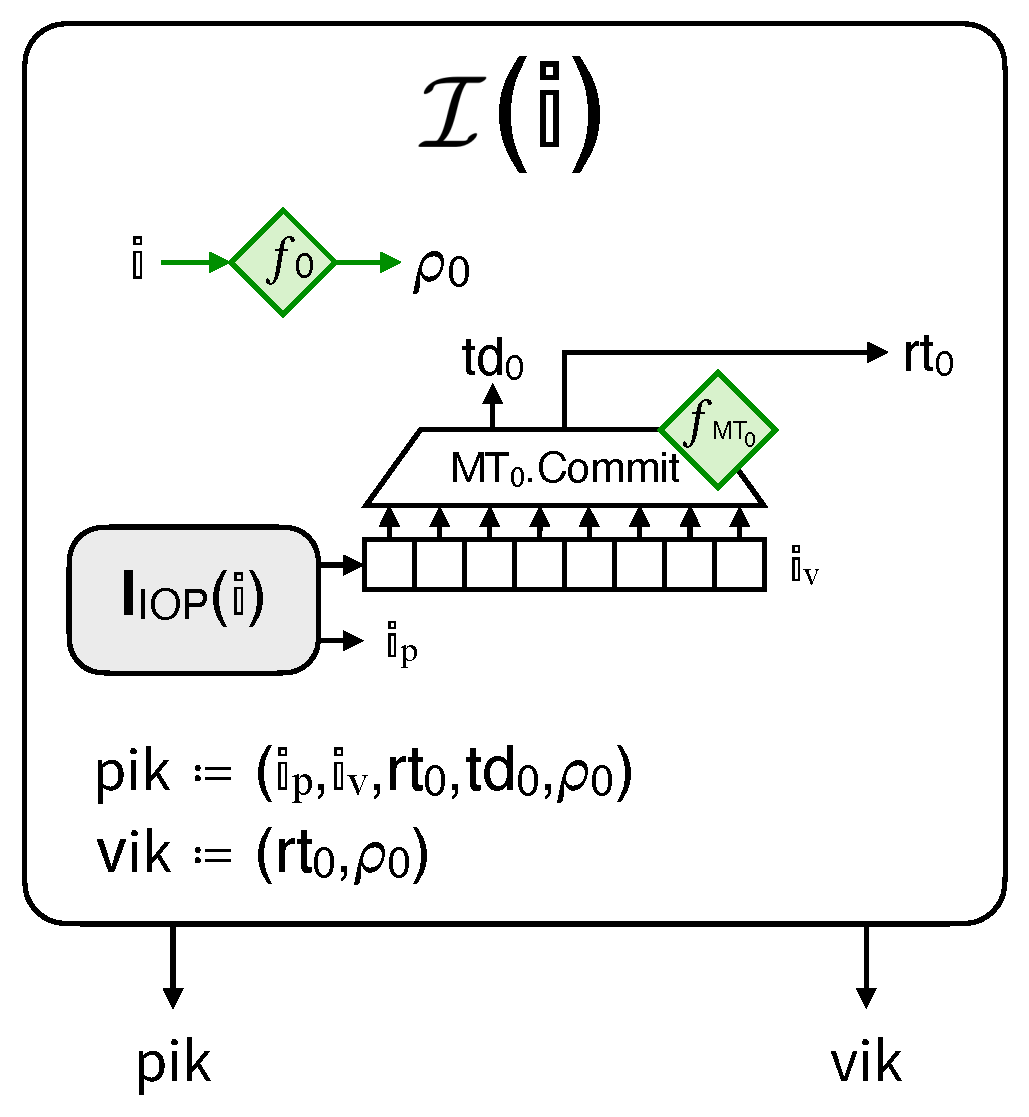
\includegraphics[width=0.4\textwidth]{\FigureFolder/cos-indexer-diagram}
\quad
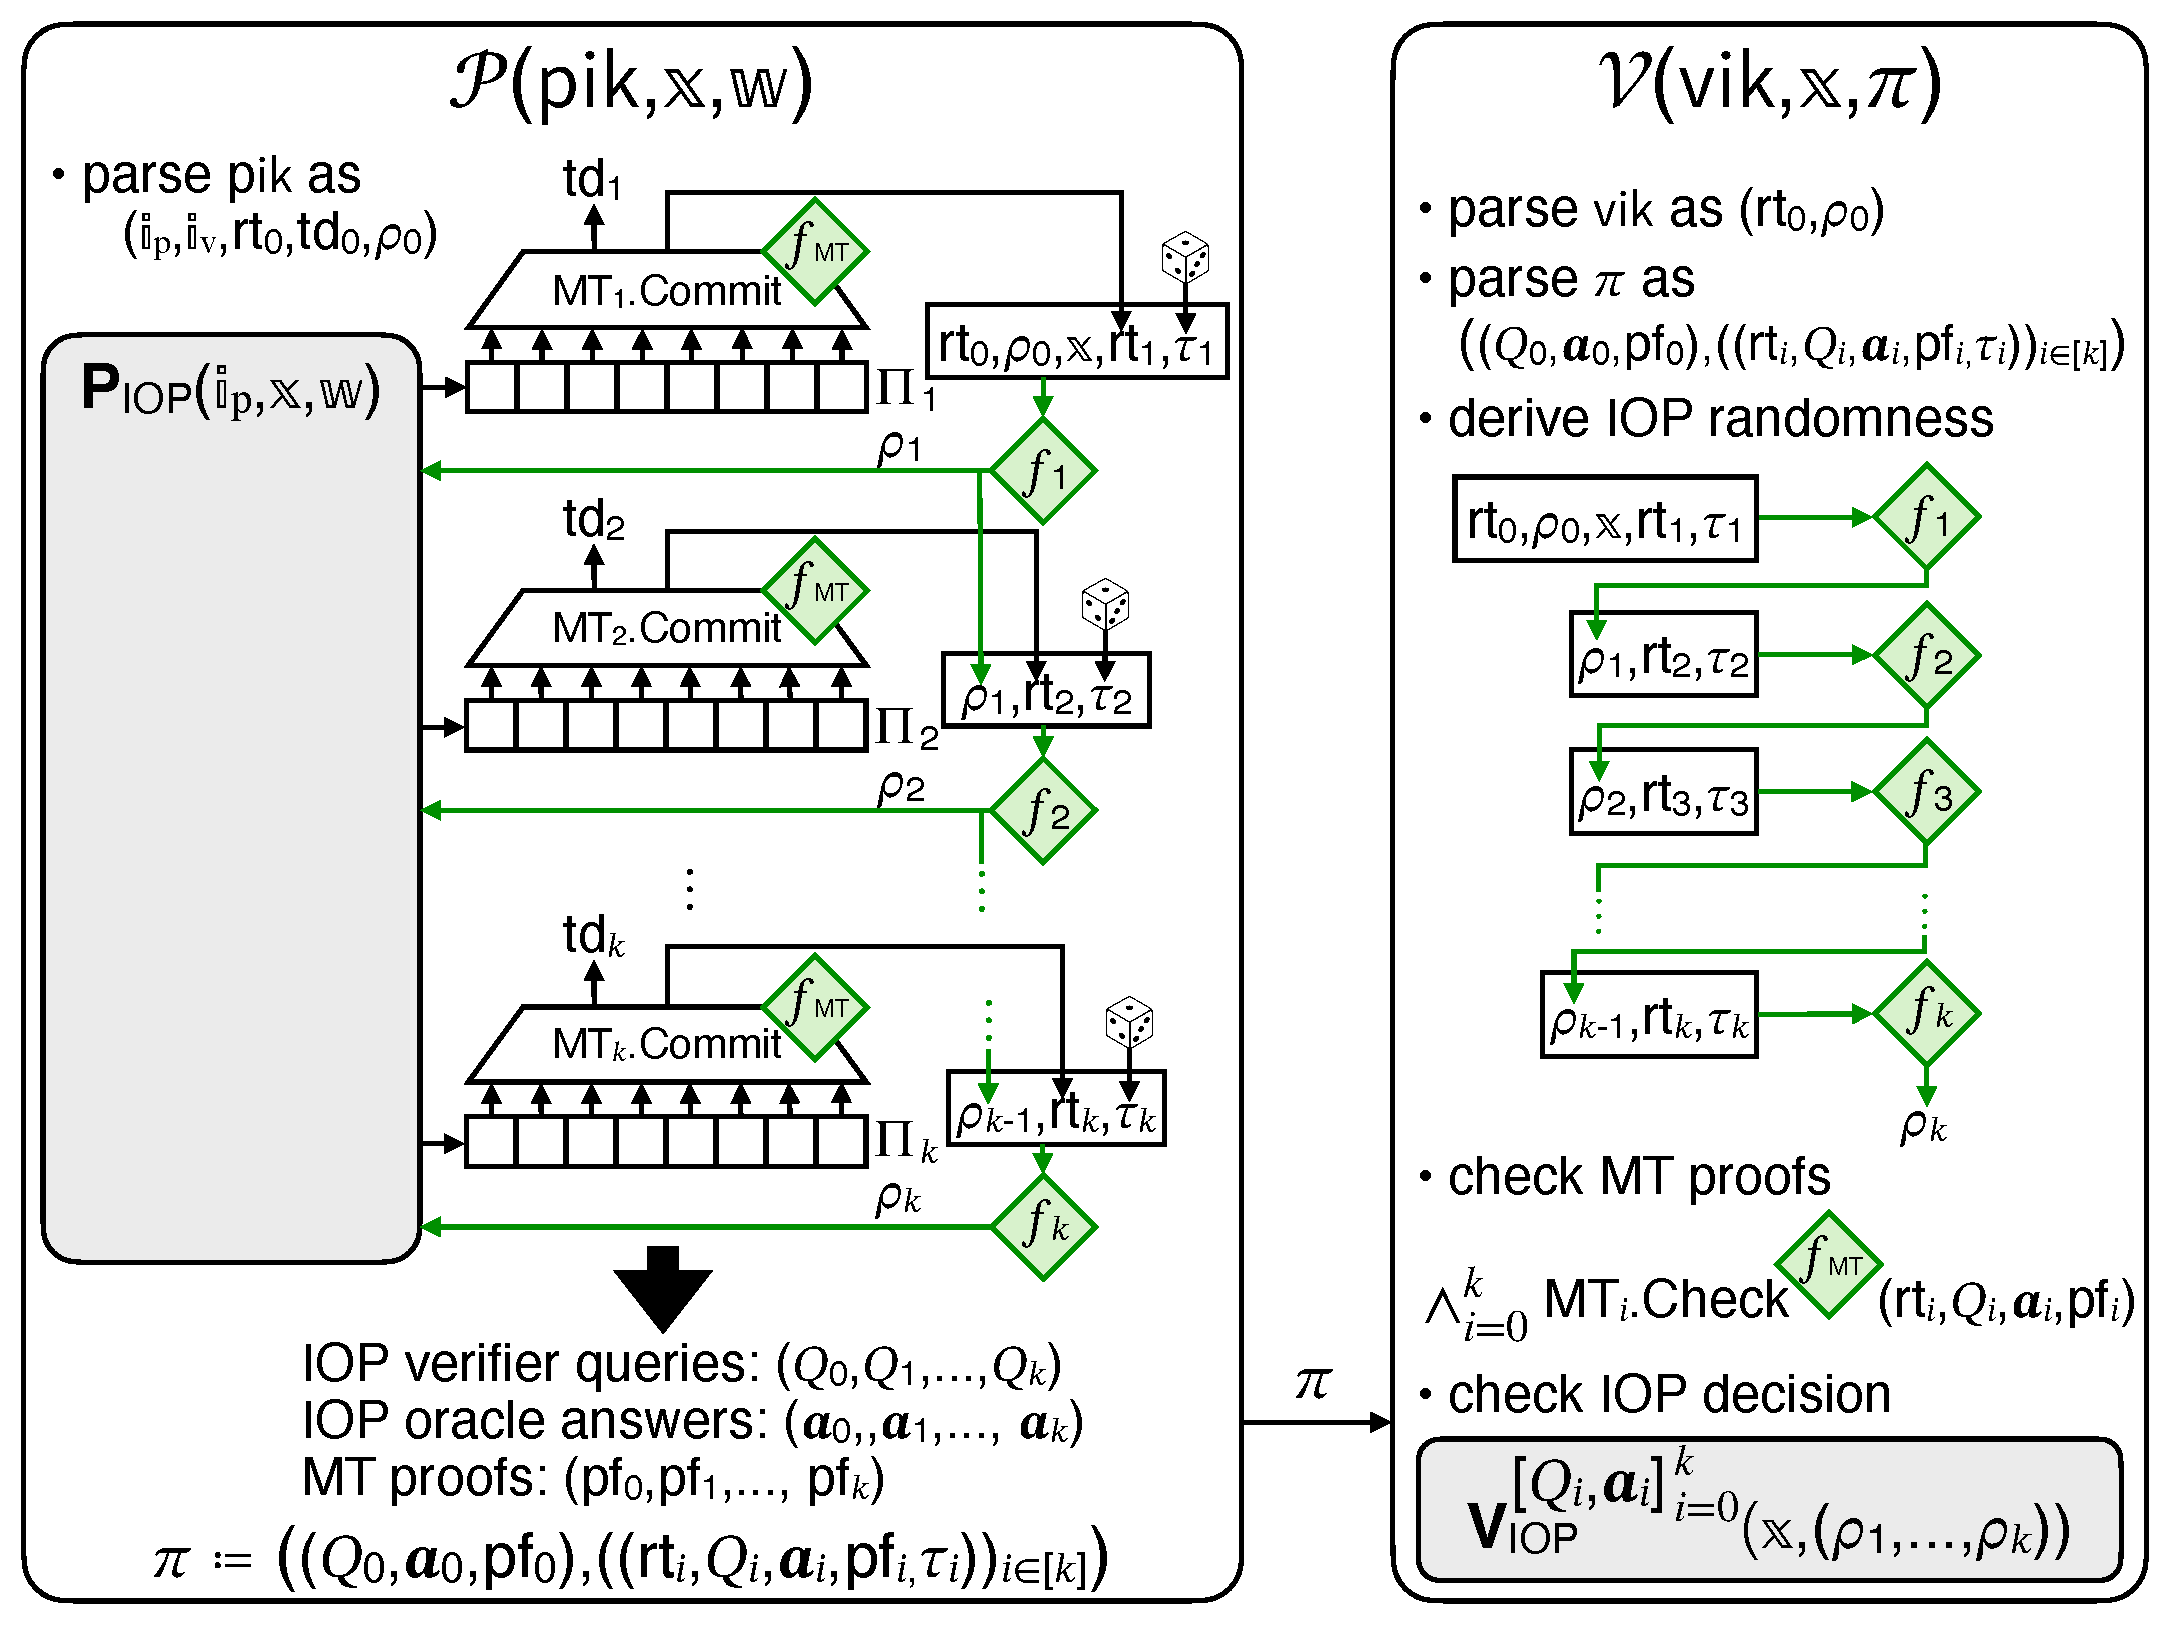
\includegraphics[width=0.8\textwidth]{\FigureFolder/cos-prover-and-verifier-diagram}
\caption[Diagram of the COS transformation]{Diagram of the \COSText ($\COSSymbol$ in \Cref{construction:cos-transformation}); the indexer is on the top and the prover and verifier are on the bottom.}
\label{figure:cos-diagram}
\end{figure}

%%%%%%%%%%%%%%%%%%%%%%%%%%%%%%%%%%%%%%%%%%%%%%%%%%%%%%%%%%%%%%%%%%%%%%%%%%%%%%%
%%%%%%%%%%%%%%%%%%%%%%%%%%%%%%%%%%%%%%%%%%%%%%%%%%%%%%%%%%%%%%%%%%%%%%%%%%%%%%%
%%%%%%%%%%%%%%%%%%%%%%%%%%%%%%%%%%%%%%%%%%%%%%%%%%%%%%%%%%%%%%%%%%%%%%%%%%%%%%%
\section{Security of the COS transformation}
\label{section:cos-security}

The COS transformation is an extension of the BCS transformation, so security properties of the COS transformation can, in general, be proved via similar approaches as for the BCS transformation. Intuitively, the soundness error and knowledge soundness error of the COS transformation incur a small additive error over the respective errors of the BCS transformation, quantifying the security of the offline phase; in contrast, the zero-knowledge error of the COS transformation is the same as that of the BCS transformation because the security of the offline phase does not affect the zero knowledge property.

\parhead{Organization}
In \Cref{section:cos-to-bcs} we describe a security reduction from the COS transformation to the BCS transformation: we show how a malicious argument prover against the COS verifier can be transformed into a corresponding malicious argument prover against the BCS verifier, up to a small additive error that quantifies the security of the offline phase. This reduction allows us to prove in \Cref{section:cos-soundness} the soundness and in \Cref{section:cos-knowledge-soundness} the knowledge soundness of the COS transformation, without \DoQuote{opening up} the analyses of the respective properties of the BCS transformation. Finally, in \Cref{section:cos-zero-knowledge} we state the zero-knowledge error and provide the simulator for the COS transformation; we omit the proof because it is a syntactic modification of that of the BCS transformation, due to the fact that the offline phase does not affect the zero-knowledge property.

%%%%%%%%%%%%%%%%%%%%%%%%%%%%%%%%%%%%%%%%%%%%%%%%%%%%%%%%%%%%%%%%%%%%%%%%%%%%%%%
%%%%%%%%%%%%%%%%%%%%%%%%%%%%%%%%%%%%%%%%%%%%%%%%%%%%%%%%%%%%%%%%%%%%%%%%%%%%%%%
%%%%%%%%%%%%%%%%%%%%%%%%%%%%%%%%%%%%%%%%%%%%%%%%%%%%%%%%%%%%%%%%%%%%%%%%%%%%%%%
\subsection{From COS to BCS}
\label{section:cos-to-bcs}

We provide a security reduction from the COS transformation to the BCS transformation, by describing how a malicious argument prover against the COS verifier can be reduced to a corresponding malicious argument prover against the BCS verifier, quantifying the security loss of this reduction.

\parhead{From HIOP to IOP}
We describe how to \DoQuote{downcast} a given holographic IOP into a corresponding (non-holographic) IOP wherein the honest prover and honest verifier each take responsibility of the offline phase. The transformation is conceptually simple, though demands some text to state precisely due to the different settings.

\begin{definition}
\label{definition:from-indexed-to-nonindexed}
Given an indexed relation $\IndexedRelation$, the corresponding (non-indexed) relation is
\begin{equation*}
\GetRelation{\IndexedRelation}
\DefineEqual
\{
((\Index,\Instance),\Witness) :
(\Index,\Instance,\Witness) \in \IndexedRelation
\}
\enspace.
\end{equation*}
\end{definition}

\begin{construction}
\label{construction:from-hiop-to-iop}
Let $\HIOPSymbol=\HIOPSystem$ be a holographic IOP for an indexed relation $\IndexedRelation$. We define a (standard) IOP $\IOPSymbol=\IOPSystem$ for the relation $\GetRelation{\IndexedRelation}$.
\begin{itemize}
  \item The IOP prover $\IOPProver$ receives as input a full instance $(\Index,\Instance)$ and a witness $\Witness$, computes the encoded indices $(\ProverEncodedIndex,\VerifierEncodedIndex) \DefineEqual \HIOPIndexer(\Index)$, and then emulates the HIOP prover $\HIOPProver$ on input $(\ProverEncodedIndex,\Instance,\Witness)$.
  \item The IOP verifier $\IOPVerifier$ receives as input a full instance $(\Index,\Instance)$, computes the encoded indices $(\ProverEncodedIndex,\VerifierEncodedIndex) \DefineEqual \HIOPIndexer(\Index)$, and then emulates the HIOP verifier $\HIOPVerifier$ given query access to $\VerifierEncodedIndex$ and input $\Instance$.
\end{itemize}
\end{construction}

The non-holographic IOP $\IOPSymbol$ derived from the holographic IOP $\HIOPSymbol$ differs in computational efficiency but is otherwise \DoQuote{equivalent} from the perspective of security, as in following lemma.

\begin{lemma}
\label{lemma:from-hiop-to-iop}
Suppose that $\HIOPSymbol$ for $\IndexedRelation$ has perfect completeness, soundness error $\HIOPSoundnessError$, straightline knowledge soundness error $\HIOPKnowledgeError$, rewinding knowledge soundness error $\HIOPKnowledgeError$ with extraction time $\HIOPKnowledgeTime$, honest-verifier zero-knowledge error $\HIOPZKError$, state-restoration soundness $\HIOPSRSoundnessError$, straightline state-restoration knowledge soundness error $\HIOPSRKnowledgeError$, and rewinding state-restoration knowledge soundness error $\HIOPSRKnowledgeError$ with extraction time $\HIOPSRKnowledgeTime$. Then $\IOPSymbol$ for $\GetRelation{\IndexedRelation}$ obtained from $\HIOPSymbol$ as in \Cref{construction:from-hiop-to-iop} has:
\begin{itemize}[nolistsep]
  \item perfect completeness;
  \item soundness error $\IOPSoundnessError((\Index,\Instance)) \leq \HIOPSoundnessError(\Index,\Instance)$;
  \item straightline knowledge soundness error $\IOPKnowledgeError((\Index,\Instance)) \leq \HIOPKnowledgeError(\Index,\Instance)$;
  \item rewinding knowledge soundness error $\IOPKnowledgeError((\Index,\Instance),\ProverFailureProbability{\IOPMaliciousProver}((\Index,\Instance))) \leq \HIOPKnowledgeError(\Index,\Instance,\ProverFailureProbability{\HIOPMaliciousProver}(\Index,\Instance))$ with extraction time $\IOPKnowledgeTime((\Index,\Instance),\ProverFailureProbability{\HIOPMaliciousProver}((\Index,\Instance)),\ProverRunningTime{\HIOPMaliciousProver}((\Index,\Instance))) \leq \HIOPKnowledgeTime(\Index,\Instance,\ProverFailureProbability{\HIOPMaliciousProver}(\Index,\Instance),\ProverRunningTime{\HIOPMaliciousProver}(\Index,\Instance))$;
  \item honest-verifier zero-knowledge error $\IOPZKError((\Index,\Instance)) \leq \HIOPZKError(\Index,\Instance)$;
  \item state-restoration soundness $\IOPSRSoundnessError(\SRSaltSize,\SRBudget,\IndexSize+\InstanceSize) \leq \HIOPSRSoundnessError(\SRSaltSize,\SRBudget,\IndexSize,\InstanceSize)$;
  \item straightline state-restoration knowledge soundness error $\IOPSRKnowledgeError(\SRSaltSize,\SRBudget,\IndexSize+\InstanceSize) \leq \HIOPSRKnowledgeError(\SRSaltSize,\SRBudget,\IndexSize,\InstanceSize)$;
  \item rewinding state-restoration knowledge soundness error $\IOPSRKnowledgeError(\SRSaltSize,\SRBudget,\IndexSize+\InstanceSize,\ProverFailureProbability{\HIOPMaliciousSRProver}(\SRSaltSize,\IndexSize+\InstanceSize)) \leq \HIOPSRKnowledgeError(\SRSaltSize,\SRBudget,\IndexSize,\InstanceSize,\ProverFailureProbability{\HIOPMaliciousSRProver}(\SRSaltSize,\IndexSize,\InstanceSize))$ with extraction time $\IOPSRKnowledgeTime(\SRSaltSize,\SRBudget,\IndexSize+\InstanceSize,\ProverFailureProbability{\HIOPMaliciousSRProver}(\SRSaltSize,\IndexSize+\InstanceSize),\ProverRunningTime{\HIOPMaliciousSRProver}(\SRSaltSize,\IndexSize+\InstanceSize)) \leq \HIOPSRKnowledgeTime(\SRSaltSize,\SRBudget,\IndexSize,\InstanceSize,\ProverFailureProbability{\HIOPMaliciousSRProver}(\SRSaltSize,\IndexSize,\InstanceSize),\ProverRunningTime{\HIOPMaliciousSRProver}(\SRSaltSize,\IndexSize,\InstanceSize))$.
\end{itemize}
\end{lemma}

\parhead{From COS to BCS}
The preprocessing NARG whose security we wish to analyze is obtained by applying the COS transformation to the holographic IOP $\HIOPSymbol$. We compare this to the (non-preprocessing) NARG obtained by applying the BCS transformation to the corresponding (non-holographic) IOP $\IOPSymbol$ from \Cref{construction:from-hiop-to-iop}. We define these two NARGs below:
\begin{align*}
  (\COSIndexer,\COSProver,\COSVerifier) &\DefineEqual \COSTransformation{\HIOPSymbol}{\SecurityParameter}{\PrivacyParameter} \enspace, \\
  (\BCSProver,\BCSVerifier) &\DefineEqual \BCSTransformation{\IOPSymbol}{\SecurityParameter}{\PrivacyParameter}
  \enspace.
\end{align*}
\Cref{construction:cos-to-bcs} explains how to transform a malicious argument prover $\Malicious{\ARGProver}_{\COSSubscript}$ against $\COSVerifier$ into a malicious argument prover $\Malicious{\ARGProver}_{\BCSSubscript}(\BlackBox{\Malicious{\ARGProver}_{\COSSubscript}})$ against $\BCSVerifier$. Then \Cref{construction:cos-to-bcs-trace} describes an algorithm $\COSToBCSTrace$ that transforms the query-answer trace of $\Malicious{\ARGProver}_{\COSSubscript}$ into the query-answer trace of $\Malicious{\ARGProver}_{\BCSSubscript}(\BlackBox{\Malicious{\ARGProver}_{\COSSubscript}})$.

\begin{construction}
\label{construction:cos-to-bcs}
Let $\Malicious{\ARGProver}_{\COSSubscript}$ a malicious argument prover against $\COSVerifier$. We construct an argument prover $\Malicious{\ARGProver}_{\BCSSubscript}$ against $\BCSVerifier$ that works as follows.
\begin{itemize}[noitemsep]
  \item[] $\Malicious{\ARGProver}_{\BCSSubscript}^{(\ROTreeFunction,(\RORandRoundFunction{\RoundIndex})_{\RoundIndex \in [\IOPRoundComplexity]})}(\BlackBox{\Malicious{\ARGProver}_{\COSSubscript}})$:
  \begin{enumerate}[nolistsep]
    \item Lazily sample an oracle $\LazyROIndexTreeFunction \gets \RODistribution{\SecurityParameter}$.
    \item Lazily sample an oracle $\LazyROIndexHashFunction \gets \RODistribution{\SecurityParameter}$.
    \item Lazily sample an oracle $\LazySub{\ROFunctionAlt}{1} \gets \RODistribution{\IOPRandomnessComplexity_{1}}$ (to answer malformed queries).
    \item Run $\Malicious{\ARGProver}_{\COSSubscript}$ until it outputs $(\Index,\AuxiliaryState)$ by answering each query $\ROQuery$ as follows.
    \begin{itemize}[nolistsep]
      \item If $\ROQuery$ is a query to $\ROIndexTreeFunction$, answer with $\ROAnswer \DefineEqual \LazyROIndexTreeFunction(\ROQuery)$.
      \item If $\ROQuery$ is a query to $\ROIndexHashFunction$, answer with $\ROAnswer \DefineEqual \LazyROIndexHashFunction(\ROQuery)$.
      \item If $\ROQuery$ is a query to $\ROTreeFunction$, answer with $\ROAnswer \DefineEqual \ROTreeFunction(\ROQuery)$.
      \item If $\ROQuery$ is a query to $\RORandRoundFunction{\RoundIndex}$ with $\RoundIndex \in \{2,\dots,\IOPRoundComplexity\}$, answer with $\ROAnswer \DefineEqual \RORandRoundFunction{\RoundIndex}(\ROQuery)$.
      \item If $\ROQuery$ is a query to $\RORandRoundFunction{1}$ then:
      \begin{enumerate}[nolistsep]
        \item parse $\ROQuery$ as a tuple $\COSFSFirstQuery$ and, if not possible, answer with $\ROAnswer \DefineEqual \LazySub{\ROFunctionAlt}{1}(\ROQuery)$;
        \item if there is a unique prior query $\ROQuery_{\IndexRoundSubscript}$ to $\ROIndexHashFunction$ whose answer is $\HashedIndex$ then answer with $\RORandRoundFunction{1}((\ROQuery_{\IndexRoundSubscript},\Instance),\MTCommitment_{1},\RandSaltString_{1})$;
        \item if there are multiple prior queries to $\ROIndexHashFunction$ whose answer is $\HashedIndex$ or there are no such queries then answer with $\ROAnswer \DefineEqual \LazySub{\ROFunctionAlt}{1}(\ROQuery)$.
      \end{enumerate}
    \end{itemize}
    \item Compute index keys: $(\ARGpik,\ARGvik) \DefineEqual \COSIndexer^{(\LazyROIndexTreeFunction,\LazyROIndexHashFunction,\ROTreeFunction,(\RORandRoundFunction{\RoundIndex})_{\RoundIndex \in [\IOPRoundComplexity]})}(\Index)$.
    \item Run $\Malicious{\ARGProver}_{\COSSubscript}(\AuxiliaryState,\ARGpik,\ARGvik)$ until it outputs $(\Instance,\ARGString_{\COSSubscript})$ by answering each query $\ROQuery$ as above.
    \item Parse the argument string $\ARGString_{\COSSubscript}$ as a tuple $\big((\IOPQuerySet_{\IndexRoundSubscript},\IOPEntries_{\IndexRoundSubscript},\MTProof_{\IndexRoundSubscript}),\ARGString_{\BCSSubscript}\big)$.
    \item Compute the bit $\DecisionBit_{\IndexRoundSubscript} \DefineEqual \MTIdxCheck{\IndexRoundSubscript}^{\ROIndexTreeFunction}(\MTCommitment_{\IndexRoundSubscript},\IOPQuerySet_{\IndexRoundSubscript},\IOPEntries_{\IndexRoundSubscript},\MTProof_{\IndexRoundSubscript})$. (The bit $\DecisionBit_{\IndexRoundSubscript}$ is not output and is used to state \Cref{lemma:cos-to-bcs}.)
    \item Output $((\Index,\Instance),\ARGString_{\BCSSubscript})$.
  \end{enumerate}
\end{itemize}
If $\Malicious{\ARGProver}_{\COSSubscript}$ makes at most $\ROTreeQueryBound$ queries to $\ROTreeFunction$ and $\RORandQueryBound$ queries to $(\RORandRoundFunction{\RoundIndex})_{\RoundIndex \in [\IOPRoundComplexity]}$, then $\Malicious{\ARGProver}_{\BCSSubscript}(\BlackBox{\Malicious{\ARGProver}_{\COSSubscript}})$ makes at most $\ROTreeQueryBound$ queries to $\ROTreeFunction$ and $\RORandQueryBound$ queries to $(\RORandRoundFunction{\RoundIndex})_{\RoundIndex \in [\IOPRoundComplexity]}$ (regardless of queries by $\Malicious{\ARGProver}_{\COSSubscript}$ to $\ROIndexTreeFunction$ and $\ROIndexHashFunction$). Moreover, the running time of $\Malicious{\ARGProver}_{\BCSSubscript}(\BlackBox{\Malicious{\ARGProver}_{\COSSubscript}})$ equals the running time of $\Malicious{\ARGProver}_{\COSSubscript}$ plus $\ARGTimeI$ (the time of $\COSIndexer$ discussed in \Cref{section:cos-transformation}) plus $\ExtraTimeofCOSToBCSProver$ (the total time to answer at most $\RORandQueryBound$ queries to $\RORandRoundFunction{1}$), where $\ROIndexHashQueryBound$ is the number of queries by $\Malicious{\ARGProver}_{\COSSubscript}$ to $\ROIndexHashFunction$. The last term stems from sorting the queries to $\ROIndexHashFunction$ and performing a lookup for each of the $\RORandQueryBound$ queries to $\RORandRoundFunction{1}$.
\end{construction}

\begin{construction}
\label{construction:cos-to-bcs-trace}
The function $\COSToBCSTrace$ receives as input a query-answer trace $\ROTrace$ for oracles $(\ROIndexTreeFunction,\ROIndexHashFunction,\ROTreeFunction,(\RORandRoundFunction{\RoundIndex})_{\RoundIndex \in [\IOPRoundComplexity]}) \in \RODistribution{(\SecurityParameter,\SecurityParameter,\SecurityParameter,\IOPTuple{\IOPRandomnessComplexity})}$ and outputs a query-answer trace $\ROTrace_{\BCSSubscript}$ for oracles $(\ROTreeFunction,(\RORandRoundFunction{\RoundIndex})_{\RoundIndex \in [\IOPRoundComplexity]}) \in \RODistribution{(\SecurityParameter,\IOPTuple{\IOPRandomnessComplexity})}$ computed as follows.
\begin{itemize}[noitemsep]
  \item[] $\COSToBCSTrace(\ROTrace)$:
  \begin{enumerate}[nolistsep]
    \item Initialize an empty list of move-response pairs $\ROTrace_{\BCSSubscript}$.
    \item For each query-answer $(\ROQuery,\ROAnswer)$ in $\ROTrace$ (taken in order):
    \begin{itemize}[nolistsep]
      \item if $\ROQuery$ is a query to $\ROIndexTreeFunction$, then do nothing;
      \item if $\ROQuery$ is a query to $\ROIndexHashFunction$, then do nothing;
      \item if $\ROQuery$ is a query to $\ROTreeFunction$, append $(\ROQuery,\ROAnswer)$ to $\ROTrace_{\BCSSubscript}$ as a query to $\ROTreeFunction$;
      \item if $\ROQuery$ is a query to $\RORandRoundFunction{\RoundIndex}$ with $\RoundIndex \in \{2,\dots,\IOPRoundComplexity\}$, append $(\ROQuery,\ROAnswer)$ to $\ROTrace_{\BCSSubscript}$ as a query to $\RORandRoundFunction{\RoundIndex}$;
      \item if $\ROQuery$ is a query to $\RORandRoundFunction{1}$ then:
      \begin{enumerate}[nolistsep]
        \item parse $\ROQuery$ as a tuple $\COSFSFirstQuery$ (if not possible then do nothing);
        \item search for all prior queries to $\ROIndexHashFunction$ whose answer is $\HashedIndex$;
        \item if a unique such query $\ROQuery_{\IndexRoundSubscript}$ is found then append $(((\ROQuery_{\IndexRoundSubscript},\Instance),\MTCommitment_{1},\RandSaltString_{1}),\ROQuery_{\IndexRoundSubscript})$ to $\ROTrace_{\BCSSubscript}$ as a query to $\RORandRoundFunction{1}$;
        \item if no such queries or more than one such query is found then do nothing.
      \end{enumerate}
    \end{itemize}
    \item Output $\ROTrace_{\BCSSubscript}$.
  \end{enumerate}
\end{itemize}
The running time of $\COSToBCSTrace$ is $\TimeofCOSToBCSTrace$, where the term $O(\IOPMaxRandomnessComplexity \cdot \ROQueryBound)$ comes from a linear pass on the queries and the term $\ExtraTimeofCOSToBCSProver$ comes from processing queries to $\RORandRoundFunction{1}$ (as explained in the last paragraph of \Cref{construction:cos-to-bcs}).
\end{construction}

\parhead{Security reduction}
The lemma below quantifies the security loss in transforming the malicious argument prover $\Malicious{\ARGProver}_{\COSSubscript}$ against $\COSVerifier$ into the malicious argument prover $\Malicious{\ARGProver}_{\BCSSubscript}(\BlackBox{\Malicious{\ARGProver}_{\COSSubscript}})$ against $\BCSVerifier$.

\begin{lemma}
\label{lemma:cos-to-bcs}
For every malicious argument prover $\Malicious{\ARGProver}_{\COSSubscript}$, the statistical distance of the two distributions
\begin{equation*}
\left\{
  (\ROTrace_{\BCSSubscript},\Index,\Instance,\ARGString_{\COSSubscript},\DecisionBit_{\COSSubscript})
\GivenExperiment
\StateExperiment{
  \ROFunction=(\ROIndexTreeFunction,\ROIndexHashFunction,\ROTreeFunction,(\RORandRoundFunction{\RoundIndex})_{\RoundIndex \in [\IOPRoundComplexity]}) \gets \RODistribution{(\SecurityParameter,\SecurityParameter,\SecurityParameter,\IOPTuple{\IOPRandomnessComplexity})} \\
  (\Index,\AuxiliaryState) \xleftarrow{\ROTrace_{1}} \Malicious{\ARGProver}_{\COSSubscript}^{\ROFunction} \\
  (\ARGpik,\ARGvik) \xleftarrow{\ROTraceIndexer} \COSIndexer^{\ROFunction}(\Index) \\
  (\Instance,\ARGString_{\COSSubscript}) \xleftarrow{\ROTrace_{2}} \Malicious{\ARGProver}_{\COSSubscript}^{\ROFunction}(\AuxiliaryState,\ARGpik,\ARGvik) \\
  \text{parse} \; \ARGString_{\COSSubscript} \; \text{as} \; \big((\IOPQuerySet_{\IndexRoundSubscript},\IOPEntries_{\IndexRoundSubscript},\MTProof_{\IndexRoundSubscript}),\ARGString_{\BCSSubscript}\big) \\
  \DecisionBit_{\COSSubscript} \xleftarrow{\ROTraceVerifier} \COSVerifier^{\ROFunction}(\ARGvik,\Instance,\ARGString) \\
  \ROTrace_{\COSSubscript} \DefineEqual \ROTrace_{1} \concat \ROTraceIndexer \concat \ROTrace_{2} \concat \ROTraceVerifier \\
  \ROTrace_{\BCSSubscript} \DefineEqual \COSToBCSTrace(\ROTrace_{\COSSubscript})
}
\right\}
\end{equation*}
and
\begin{equation*}
\left\{
  (\ROTrace \concat \ROTraceVerifier,\Index,\Instance,\ARGString_{\BCSSubscript},\DecisionBit_{\BCSSubscript} \land \DecisionBit_{\IndexRoundSubscript})
\GivenExperiment
\StateExperiment{
  \ROFunction=(\ROTreeFunction,(\RORandRoundFunction{\RoundIndex})_{\RoundIndex \in [\IOPRoundComplexity]}) \gets \RODistribution{(\SecurityParameter,\IOPTuple{\IOPRandomnessComplexity})} \\
  ((\Index,\Instance),\ARGString_{\BCSSubscript}) \xleftarrow{\ROTrace,\DecisionBit_{\IndexRoundSubscript}} \Malicious{\ARGProver}_{\BCSSubscript}^{\ROFunction}(\BlackBox{\Malicious{\ARGProver}_{\COSSubscript}}) \\
  \DecisionBit_{\BCSSubscript} \xleftarrow{\ROTraceVerifier} \BCSVerifier^{\ROFunction}((\Index,\Instance),\ARGString_{\BCSSubscript})
}
\right\}
\enspace.
\end{equation*}
is at most
\begin{equation*}
\COSErrorExpression
\enspace.
\end{equation*}
Above, $\ROIndexTreeQueryBound$ and $\ROIndexHashQueryBound$ are bounds on the number of queries by $\Malicious{\ARGProver}_{\COSSubscript}$ to the oracles $\ROIndexTreeFunction$ and $\ROIndexHashFunction$.
\end{lemma}

\begin{proof}
We define two events over the the probability space of the top experiment:
\begin{itemize}[noitemsep]
  \item $\Event_{1}$ holds if $\MTIdxCheck{\IndexRoundSubscript}^{\ROIndexTreeFunction}(\MTCommitment_{\IndexRoundSubscript},\IOPQuerySet_{\IndexRoundSubscript},\IOPEntries_{\IndexRoundSubscript},\MTProof_{\IndexRoundSubscript})=1$ and $\IOPEntries_{\IndexRoundSubscript} \neq \VerifierEncodedIndex[\IOPQuerySet_{\IndexRoundSubscript}]$.
  \item $\Event_{2}$ holds if $\ROTrace_{\COSSubscript}$ contains more than one query to $\ROIndexHashFunction$ whose answer is $\HashedIndex$ (at least one query exists because $\ROTraceIndexer$ contains the pair $(\Index,\HashedIndex)$).
\end{itemize}
Here $\HashedIndex$ refers to the index output by $\Malicious{\ARGProver}_{\COSSubscript}$ and $\VerifierEncodedIndex$ refers to the verifier encoded index in $\ARGpik$. It suffices to upper bound the probability that $\Event_{1} \lor \Event_{2}$ holds and showing that the following two distributions are identical:
\begin{equation*}
\left\{
\begin{array}{l}
  (\ROTrace_{\BCSSubscript},\Index,\Instance,\ARGString_{\BCSSubscript},\DecisionBit_{\COSSubscript}) \\
  \ConditionedOnText \\
  \Negate{\Event_{1} \lor \Event_{2}}
\end{array}
\GivenExperiment
\StateExperiment{
  \ROFunction=(\ROIndexTreeFunction,\ROIndexHashFunction,\ROTreeFunction,(\RORandRoundFunction{\RoundIndex})_{\RoundIndex \in [\IOPRoundComplexity]}) \gets \RODistribution{(\SecurityParameter,\SecurityParameter,\SecurityParameter,\IOPTuple{\IOPRandomnessComplexity})} \\
  (\Index,\AuxiliaryState) \xleftarrow{\ROTrace_{1}} \Malicious{\ARGProver}_{\COSSubscript}^{\ROFunction} \\
  (\ARGpik,\ARGvik) \xleftarrow{\ROTraceIndexer} \COSIndexer^{\ROFunction}(\Index) \\
  (\Instance,\ARGString_{\COSSubscript}) \xleftarrow{\ROTrace_{2}} \Malicious{\ARGProver}_{\COSSubscript}^{\ROFunction}(\AuxiliaryState,\ARGpik,\ARGvik) \\
  \text{parse} \; \ARGString_{\COSSubscript} \; \text{as} \; \big((\IOPQuerySet_{\IndexRoundSubscript},\IOPEntries_{\IndexRoundSubscript},\MTProof_{\IndexRoundSubscript}),\ARGString_{\BCSSubscript}\big) \\
  \DecisionBit_{\COSSubscript} \xleftarrow{\ROTraceVerifier} \COSVerifier^{\ROFunction}(\ARGvik,\Instance,\ARGString) \\
  \ROTrace_{\COSSubscript} \DefineEqual \ROTrace_{1} \concat \ROTraceIndexer \concat \ROTrace_{2} \concat \ROTraceVerifier \\
  \ROTrace_{\BCSSubscript} \DefineEqual \COSToBCSTrace(\ROTrace_{\COSSubscript})
}
\right\}
\end{equation*}
and
\begin{equation*}
\left\{
\begin{array}{l}
  (\ROTrace \concat \ROTraceVerifier,\Index,\Instance,\ARGString_{\BCSSubscript},\DecisionBit_{\BCSSubscript} \land \DecisionBit_{\IndexRoundSubscript}) \\
  \ConditionedOnText \\
  \Negate{\Event_{1} \lor \Event_{2}}
\end{array}
\GivenExperiment
\StateExperiment{
  \ROFunction=(\ROTreeFunction,(\RORandRoundFunction{\RoundIndex})_{\RoundIndex \in [\IOPRoundComplexity]}) \gets \RODistribution{(\SecurityParameter,\IOPTuple{\IOPRandomnessComplexity})} \\
  ((\Index,\Instance),\ARGString_{\BCSSubscript}) \xleftarrow{\ROTrace,\DecisionBit_{\IndexRoundSubscript}} \Malicious{\ARGProver}_{\BCSSubscript}^{\ROFunction}(\BlackBox{\Malicious{\ARGProver}_{\COSSubscript}}) \\
  \DecisionBit_{\BCSSubscript} \xleftarrow{\ROTraceVerifier} \BCSVerifier^{\ROFunction}((\Index,\Instance),\ARGString_{\BCSSubscript})
}
\right\}
\enspace.
\end{equation*}
Below we refer to the two experiments as the top experiment and the bottom experiment. Both experiments involve the execution (or emulation) of $\Malicious{\ARGProver}_{\COSSubscript}$; in particular, $\Event_{1}$ and $\Event_{2}$ are well-defined also for the bottom experiment.

First we argue that the distribution of $(\Index,\Instance,\ARGString_{\BCSSubscript})$ is identical in both experiments (given the conditioning). In the top experiment $\Malicious{\ARGProver}_{\COSSubscript}$ outputs the index $\Index$ in its first computation phase and then additionally outputs $(\Instance,\ARGString_{\BCSSubscript})$ in its second computation phase ($\ARGString_{\BCSSubscript}$ is contained in $\ARGString_{\COSSubscript}$), after receiving the index keys. In the bottom experiment, $\Malicious{\ARGProver}_{\BCSSubscript}(\BlackBox{\Malicious{\ARGProver}_{\COSSubscript}})$ outputs $(\Index,\Instance,\ARGString_{\BCSSubscript})$ obtained by emulating the two computation phases of $\Malicious{\ARGProver}_{\COSSubscript}$. Therefore, it suffices to argue that the view of $\Malicious{\ARGProver}_{\COSSubscript}$ is identical in both experiments; the view of $\Malicious{\ARGProver}_{\COSSubscript}$ consists of answers to its queries and the input $(\ARGpik,\ARGvik)$ provided by $\COSIndexer^{\ROFunction}(\Index)$. We argue this by discussing how oracle queries are answered.
\begin{itemize}
  \item In both experiments queries to the oracles $\ROTreeFunction,\RORandRoundFunction{2},\dots,\RORandRoundFunction{\IOPRoundComplexity}$ are answered identically, as these oracles are sampled and used in the same way.
  \item We discuss queries to the oracles $\ROIndexTreeFunction,\ROIndexHashFunction$. In the top experiment, $\Malicious{\ARGProver}_{\COSSubscript}$ and $\COSIndexer$ directly query the oracles $\ROIndexTreeFunction$ and $\ROIndexHashFunction$, and in the bottom experiment $\Malicious{\ARGProver}_{\COSSubscript}$ and $\COSIndexer$ query oracles $\LazyROIndexTreeFunction$ and $\LazyROIndexHashFunction$ lazily sampled by $\Malicious{\ARGProver}_{\BCSSubscript}(\BlackBox{\Malicious{\ARGProver}_{\COSSubscript}})$.
  \item We discuss queries to the oracle $\RORandRoundFunction{1}$, which is the \DoQuote{interesting} case of this argument. In the top experiment, $\Malicious{\ARGProver}_{\COSSubscript}$ and $\COSIndexer$ directly query the oracle $\RORandRoundFunction{1}$. In the bottom experiment, the queries by $\Malicious{\ARGProver}_{\COSSubscript}$ and $\COSIndexer$ to $\RORandRoundFunction{1}$ are answered in a special way. Queries that cannot be parsed as a certain tuple are answered via a lazily sampled oracle $\LazySub{\ROFunctionAlt}{1}$, which has the same distribution as in the top experiment.

  Queries that can be parsed are answered with $\RORandRoundFunction{1}$ if there is a unique prior query $\ROQuery_{\IndexRoundSubscript}$ whose answer is $\HashedIndex$. This is always the case since we assumed that event $\Event_{2}$ does not hold (and since one such query must exist). Thus, each such unique query $\COSFSFirstQuery$ is mapped to a unique query $(\ROQuery_{\IndexRoundSubscript},\Instance,\MTCommitment_{1},\RandSaltString_{1})$ to $\RORandRoundFunction{1}$, which means that these queries are answered consistently and uniformly by $\RORandRoundFunction{1}$.

  To summarize, all queries that can be parsed are answered consistently by $\RORandRoundFunction{1}$ and thus get random answers as in the top experiment, and all the rest are answered consistently by $\LazySub{\ROFunctionAlt}{1}$.
\end{itemize}

Next, we additionally consider the bit: we argue that $(\Index,\Instance,\ARGString_{\BCSSubscript},\DecisionBit_{\COSSubscript})$ in the top experiment and $(\Index,\Instance,\ARGString_{\BCSSubscript},\DecisionBit_{\BCSSubscript} \land \DecisionBit_{\IndexRoundSubscript})$ in the bottom experiment are identically distributed (given the conditioning).
\begin{itemize}[nolistsep]
  \item In the top experiment, $\COSVerifier^{\ROFunction}(\ARGvik,\Instance,\ARGString)$ checks that $\MTIdxCheck{\IndexRoundSubscript}^{\ROIndexTreeFunction}(\MTCommitment_{\IndexRoundSubscript},\IOPQuerySet_{\IndexRoundSubscript},\IOPEntries_{\IndexRoundSubscript},\MTProof_{\IndexRoundSubscript})=1$. In the bottom experiment, this check is captured by the bit $\DecisionBit_{\IndexRoundSubscript}$, computed by $\Malicious{\ARGProver}_{\BCSSubscript}^{\ROFunction}(\BlackBox{\Malicious{\ARGProver}_{\COSSubscript}})$ outside of $\BCSVerifier^{\ROFunction}((\Index,\Instance),\ARGString_{\BCSSubscript})$.
  \item If $\MTIdxCheck{\IndexRoundSubscript}^{\ROIndexTreeFunction}(\MTCommitment_{\IndexRoundSubscript},\IOPQuerySet_{\IndexRoundSubscript},\IOPEntries_{\IndexRoundSubscript},\MTProof_{\IndexRoundSubscript})=0$ then $\DecisionBit_{\COSSubscript}=0$, so $\DecisionBit_{\BCSSubscript} \land \DecisionBit_{\IndexRoundSubscript} = \DecisionBit_{\BCSSubscript} \land 0 = 0 = \DecisionBit_{\COSSubscript}$.
  \item If $\MTIdxCheck{\IndexRoundSubscript}^{\ROIndexTreeFunction}(\MTCommitment_{\IndexRoundSubscript},\IOPQuerySet_{\IndexRoundSubscript},\IOPEntries_{\IndexRoundSubscript},\MTProof_{\IndexRoundSubscript})=1$ then, since $\Event_{1}$ does not hold, $\IOPEntries_{\IndexRoundSubscript} = \VerifierEncodedIndex[\IOPQuerySet_{\IndexRoundSubscript}]$, which means that $\DecisionBit_{\COSSubscript}=\DecisionBit_{\BCSSubscript}$ because the remaining checks in $\COSVerifier^{\ROFunction}(\ARGvik,\Instance,\ARGString)$ and the checks in $\BCSVerifier^{\ROFunction}((\Index,\Instance),\ARGString_{\BCSSubscript})$ are equivalent. Hence $\DecisionBit_{\BCSSubscript} \land \DecisionBit_{\IndexRoundSubscript} = \DecisionBit_{\BCSSubscript} \land 1 = \DecisionBit_{\BCSSubscript} = \DecisionBit_{\COSSubscript}$.
\end{itemize}

Finally, we compare the distribution of $\ROTrace_{\BCSSubscript} \DefineEqual \COSToBCSTrace(\ROTrace_{1} \concat \ROTraceIndexer \concat \ROTrace_{2} \concat \ROTraceVerifier)$ in the top experiment and $\ROTrace \concat \ROTraceVerifier$ in the bottom experiment. The query-answer trace $\ROTrace$ of $\Malicious{\ARGProver}_{\BCSSubscript}^{\ROFunction}(\BlackBox{\Malicious{\ARGProver}_{\COSSubscript}})$ is distributed identically as a prefix of $\ROTrace_{\BCSSubscript}$ because $\COSToBCSTrace$ translates $\ROTrace_{1} \concat \ROTraceIndexer \concat \ROTrace_{2}$ in the same way that $\Malicious{\ARGProver}_{\BCSSubscript}$ emulates queries and answers for $\Malicious{\ARGProver}_{\COSSubscript}$ and $\COSIndexer$. Moreover, the query-answer trace $\ROTraceVerifier$ is distributed identically as the suffix in $\ROTrace_{\BCSSubscript}$ (corresponding to the translation by $\COSToBCSTrace$ of the suffix $\ROTraceVerifier$ in $\ROTrace_{1} \concat \ROTraceIndexer \concat \ROTrace_{2} \concat \ROTraceVerifier$), as we now explain.
\begin{itemize}[nolistsep]
  \item $\BCSVerifier^{\ROFunction}((\Index,\Instance),\ARGString_{\BCSSubscript})$ performs queries $\ROTreeFunction$ to check the Merkle opening proofs and also performs one query to each of $(\RORandRoundFunction{\RoundIndex})_{\RoundIndex \in [\IOPRoundComplexity]}$ to recover the IOP verifier random challenges.
  \item Queries to $\ROTreeFunction$ are performed the same way by $\COSVerifier$ and $\BCSVerifier$ and, consistent with this, $\COSToBCSTrace$ preserves them as is.
  \item For every $\RoundIndex \in \{2,\dots,\IOPRoundComplexity\}$, the query to $\RORandRoundFunction{\RoundIndex}$ is performed the same way by $\COSVerifier$ and $\BCSVerifier$ and, consistent with this, $\COSToBCSTrace$ preserves them as is.
  \item The query to $\RORandRoundFunction{1}$ differs in $\COSVerifier$ and $\BCSVerifier$, and $\COSToBCSTrace$ translates this query in a manner that is consistent with this difference.
\end{itemize}

We are left to upper bound the probability of the event $\Event_{1} \lor \Event_{2}$, for which we separately upper bound $\Pr[\Event_{1}]$ and $\Pr[\Event_{2}]$.
\begin{itemize}

  \item We argue that $\Pr[\Event_{1}] \leq \MTHonestBindingExpression{\SecurityParameter}{\ROIndexTreeQueryBound}{\IOPProofLength_{\IndexRoundSubscript}}$. This directly follows from \Cref{lemma:mt-other-binding} via the following adversary $\MTAdversary$ for the experiment therein.
\begin{itemize}[noitemsep]
  \item[] $\MTAdversary^{\ROIndexTreeFunction}$:
  \begin{enumerate}[nolistsep]
    \item Lazily sample an oracle $\LazyROIndexHashFunction \gets \RODistribution{\SecurityParameter}$.
    \item Lazily sample an oracle $\LazyROTreeFunction \gets \RODistribution{\SecurityParameter}$.
    \item For every $\RoundIndex \in [\IOPRoundComplexity]$, lazily sample an oracle $\LazySub{\ROFunction}{\RoundIndex} \gets \RODistribution{\IOPRandomnessComplexity_{\RoundIndex}}$.
    \item Compute $(\Index,\AuxiliaryState) \gets \Malicious{\ARGProver}_{\COSSubscript}^{(\ROIndexTreeFunction,\LazyROIndexHashFunction,\LazyROTreeFunction,(\LazySub{\ROFunction}{\RoundIndex})_{\RoundIndex \in [\IOPRoundComplexity]})}$.
    \item Set $\AuxiliaryState' \DefineEqual (\AuxiliaryState,\LazyROIndexHashFunction,\LazyROTreeFunction,(\LazySub{\ROFunction}{\RoundIndex})_{\RoundIndex \in [\IOPRoundComplexity]})$.
    \item Output $(\Index,\AuxiliaryState')$.
  \end{enumerate}
  \item[]
  \item[] $\MTAdversary^{\ROIndexTreeFunction}(\ROAdvState',\MTCommitment_{\IndexRoundSubscript},\MTTrapdoor_{\IndexRoundSubscript})$:
  \begin{enumerate}[nolistsep]
    \item Parse $\ROAdvState'$ as $(\AuxiliaryState,\LazyROIndexHashFunction,\LazyROTreeFunction,(\LazySub{\ROFunction}{\RoundIndex})_{\RoundIndex \in [\IOPRoundComplexity]})$.
    \item Set $\HashedIndex \DefineEqual \LazyROIndexHashFunction(\Index)$.
    \item Compute $(\ProverEncodedIndex,\VerifierEncodedIndex) \DefineEqual \HIOPIndexer(\Index)$.
    \item Set $\ARGpik \DefineEqual (\ProverEncodedIndex,\VerifierEncodedIndex,\MTTrapdoor_{\IndexRoundSubscript},\HashedIndex)$ and $\ARGvik \DefineEqual (\MTCommitment_{\IndexRoundSubscript},\HashedIndex)$.
    \item Compute $(\Instance,\ARGString_{\COSSubscript}) \gets \Malicious{\ARGProver}_{\COSSubscript}^{(\ROIndexTreeFunction,\LazyROIndexHashFunction,\LazyROTreeFunction,(\LazySub{\ROFunction}{\RoundIndex})_{\RoundIndex \in [\IOPRoundComplexity]})}(\AuxiliaryState,\ARGpik,\ARGvik)$.
    \item Parse $\ARGString_{\COSSubscript}$ as $\big((\IOPQuerySet_{\IndexRoundSubscript},\IOPEntries_{\IndexRoundSubscript},\MTProof_{\IndexRoundSubscript}),\ARGString_{\BCSSubscript}\big)$.
    \item Output $(\IOPQuerySet_{\IndexRoundSubscript},\IOPEntries_{\IndexRoundSubscript},\MTProof_{\IndexRoundSubscript})$.
  \end{enumerate}
\end{itemize}
The malicious argument prover $\Malicious{\ARGProver}_{\COSSubscript}$ makes at most $\ROIndexTreeQueryBound$ queries to $\ROIndexTreeFunction$ (across its two computation phases), so $\MTAdversary$ makes at most $\ROIndexTreeQueryBound$ queries to $\ROIndexTreeFunction$.

\item We argue that $\Pr[\Event_{2}] \leq \frac{1}{2} \cdot \frac{\ROIndexHashQueryBound^2}{2^{\SecurityParameter}}$. The event $\Event_{2}$ implies a collision in the query-answer trace $\ROTrace_{\COSSubscript} = \ROTrace_{1} \concat \ROTraceIndexer \concat \ROTrace_{2} \concat \ROTraceVerifier$. By \Cref{lemma:rom-cr} we can bound the probability of $\Event_{2}$ by $\ROCRExpression{\SecurityParameter}{\Cardinality{\ROTrace_{\COSSubscript}}}$. Instead, we perform a more careful analysis that yields a better upper bound, using the fact that not all queries in $\ROTrace_{\COSSubscript}$ contribute towards the probability of $\Event_{2}$ in the same way.

The event $\Event_{2}$ implies a collision specifically for the oracle $\ROIndexHashFunction$. Note that $\COSVerifier$ does not query $\ROIndexHashFunction$, so $\ROTraceVerifier$ in $\ROTrace_{\COSSubscript}$ does not contribute towards the probability of $\Event_{2}$; moreover, $\COSIndexer$ makes exactly one query to $\ROIndexHashFunction$, namely, it queries $\Index$ to obtain the answer $\HashedIndex$.

First, we bound the probability that $\ROTrace_{1}$ contains a collision. Letting $\ROQueryBound_{\IndexRoundSubscript,1}$ be the number of query-answers pairs for $\ROIndexHashFunction$ in $\ROTrace_{1}$, by \Cref{lemma:rom-cr} the probability that $\ROTrace_{1}$ contains a collision for $\ROIndexHashFunction$ is at most $\ROCRExpression{\SecurityParameter}{\ROQueryBound_{\IndexRoundSubscript,1}}$.

The query-answer trace $\ROTrace_{1}$ is followed by the query-answer trace $\ROTraceIndexer$, which fixes the value $\HashedIndex$ (if not already by $\ROTrace_{1}$). The probability that this query causes a collision is at most $\frac{1}{2^{\SecurityParameter}}$.

Thereafter, every fresh query to $\ROIndexHashFunction$ in $\ROTrace_{2}$ equals $\HashedIndex$ with probability $2^{-\SecurityParameter}$. Letting $\ROQueryBound_{\IndexRoundSubscript,2}$ be the number of query-answer pairs for $\ROIndexHashFunction$ in $\ROTrace_{2}$, the probability that this happens for any query in to $\ROIndexHashFunction$ in $\ROTrace_{1}$ is, by a union bound, at most $\frac{\ROQueryBound_{\IndexRoundSubscript,2}}{2^{\SecurityParameter}}$.

Overall, noting that $\ROIndexHashQueryBound = \ROQueryBound_{\IndexRoundSubscript,1} + \ROQueryBound_{\IndexRoundSubscript,2}$ is the total number of query-answer pairs by $\Malicious{\ARGProver}_{\COSSubscript}$ to $\ROIndexHashFunction$, we deduce the following upper bound:
\begin{align*}
\Pr[\Event_{2}] & \leq
\ROCRExpression{\SecurityParameter}{\ROQueryBound_{\IndexRoundSubscript,1}}
+ \frac{1}{2^{\SecurityParameter}}
+ \frac{\ROQueryBound_{\IndexRoundSubscript,2}}{2^{\SecurityParameter}}
\\ & =
\ROCRExpression{\SecurityParameter}{\ROQueryBound_{\IndexRoundSubscript,1}}
+ \frac{1}{2^{\SecurityParameter}}
+ \frac{\ROIndexHashQueryBound - \ROQueryBound_{\IndexRoundSubscript,1}}{2^{\SecurityParameter}}
\\ & =
\frac{1}{2} \cdot \frac{\ROQueryBound_{\IndexRoundSubscript,1}^{2} - 3\ROQueryBound_{\IndexRoundSubscript,1} + 2\ROIndexHashQueryBound + 2}{2^{\SecurityParameter}}
\\ & \leq
\frac{1}{2} \cdot \frac{\ROIndexHashQueryBound^{2} - 3\ROIndexHashQueryBound + 2\ROIndexHashQueryBound+2}{2^{\SecurityParameter}}
\EquationComment{we assume that $\ROIndexHashQueryBound \geq 3$}
\\ & =
\ROCRExpression{\SecurityParameter}{\ROIndexHashQueryBound} + \frac{1}{2^{\SecurityParameter}}
\\ & \leq
\frac{1}{2} \cdot \frac{\ROIndexHashQueryBound^2}{2^{\SecurityParameter}}
\enspace.
\end{align*}
\end{itemize}
\end{proof}

\begin{remark}[simpler error term when extending iBCS]
\label{remark:cos-for-ibcs}
The COS transformation can be simplified to extend the iBCS transformation in order to construct a preprocessing \emph{interactive} argument from a holographic IOP (see \Cref{section:from-holography-to-preprocessing} and \Cref{footnote:cos-for-ibcs-simplifies}). One can perform a security reduction similar to the one in this section, yielding a security loss of only $\MTHonestBindingExpression{\SecurityParameter}{\ROIndexTreeQueryBound}{\IOPProofLength_{\IndexRoundSubscript}}$. Indeed, the other error term $\frac{1}{2} \cdot \frac{\ROIndexHashQueryBound^2}{2^{\SecurityParameter}}$ disappears because there is no longer a need to hash the index $\Index$ (the Fiat--Shamir transformation is not used in the iBCS transformation); in particular, the random oracle $\ROIndexHashFunction$ is no longer needed (and there is no $\HashedIndex$ to include in $\ARGpik$ and $\ARGvik$).
\end{remark}

\begin{remark}[the case of Micali and Kilian]
\label{remark:cos-for-other-transformations}
The ideas underlying the COS transformation can be similarly applied to the Micali transformation, yielding a preprocessing NARG obtained from a holographic PCP; a security reduction similar to \Cref{lemma:cos-to-bcs} holds for that case, yielding the very same error term. Moreover, the simplification for extending the iBCS transformation to the preprocessing case applies to extending the Kilian transformation to the preprocessing case, yielding the very same error term mentioned in \Cref{remark:cos-for-ibcs}.
\end{remark}

%%%%%%%%%%%%%%%%%%%%%%%%%%%%%%%%%%%%%%%%%%%%%%%%%%%%%%%%%%%%%%%%%%%%%%%%%%%%%%%
%%%%%%%%%%%%%%%%%%%%%%%%%%%%%%%%%%%%%%%%%%%%%%%%%%%%%%%%%%%%%%%%%%%%%%%%%%%%%%%
%%%%%%%%%%%%%%%%%%%%%%%%%%%%%%%%%%%%%%%%%%%%%%%%%%%%%%%%%%%%%%%%%%%%%%%%%%%%%%%
\subsection{Soundness}
\label{section:cos-soundness}

We prove that \Cref{construction:cos-transformation} is adaptively sound. The following theorem states that the adaptive soundness error of the preprocessing non-interactive argument is upper bounded by the IOP state-restoration soundness error of the underlying holographic IOP plus a small error term. The error term has two parts: one part represents the probability of \DoQuote{breaking} the Merkle commitment scheme used to commit to IOP strings; and the other part represents the probability of \DoQuote{breaking} the hash-chain of IOP randomness strings or the Merkle tree used to commit to the verifier encoded index. The fact that the upper bound depends on the HIOP state-restoration soundness error, rather than the HIOP (standard) soundness error, is expected, due to the use of the Fiat--Shamir transformation.

\begin{theorem}
\label{theorem:cos-soundness}
Let $\HIOPSymbol$ be a public-coin holographic IOP for an indexed relation $\IndexedRelation$ with state-restoration soundness error $\HIOPSRSoundnessError$ (see \Cref{definition:hiop-state-restoration-soundness}), round complexity $\IOPRoundComplexity$, and proof length $\IOPProofLength$. For every security parameter $\SecurityParameter \in \Naturals$ and privacy parameter $\PrivacyParameter \in \Naturals$, $\PNARGSymbol \DefineEqual \COSTransformation{\HIOPSymbol}{\SecurityParameter}{\PrivacyParameter}$ in \Cref{construction:cos-transformation} is a preprocessing non-interactive argument for $\IndexedRelation$ with adaptive soundness error $\ARGSoundnessError$ (see \Cref{definition:preprocessing-narg-adaptive-soundness-with-cnf}) such that
\begin{equation*}
\ARGSoundnessError(\SecurityParameter,\ROQueryBound,\IndexSize,\InstanceSize)
\leq
\COSSoundnessExpression
\enspace.
\end{equation*}
Above $\MTMultiMultiExtractionError$ is the Merkle commitment multi-extraction error from \Cref{lemma:mt-multi-configuration-multi-extractability}. If $\MTMultiMultiExtractabilityCondition{\ROQueryBound}{\IOPRoundComplexity}{\log\IOPProofLength}$ and $\COSCondition$, then $\ARGSoundnessError(\SecurityParameter,\ROQueryBound,\IndexSize,\InstanceSize) \leq \HIOPSRSoundnessError(\SecurityParameter+\RandSaltSize,\ROQueryBound,\IndexSize,\InstanceSize) + \COSSimplifiedError$.
\end{theorem}

\begin{proof}
We use the results in \Cref{section:cos-to-bcs} to reduce to the adaptive soundness error of the BCS transformation, incurring a small additive error (capturing the security of the offline phase).

Recall that $(\COSIndexer,\COSProver,\COSVerifier) = \COSTransformation{\HIOPSymbol}{\SecurityParameter}{\PrivacyParameter}$ and $(\BCSProver,\BCSVerifier) = \BCSTransformation{\IOPSymbol}{\SecurityParameter}{\PrivacyParameter}$, where $\IOPSymbol$ is the IOP for the (non-indexed) relation $\GetRelation{\IndexedRelation}$ that corresponds to $\HIOPSymbol$ for $\IndexedRelation$ (see \Cref{construction:from-hiop-to-iop}). Below we consider a malicious prover $\Malicious{\ARGProver}_{\COSSubscript}$ against $\COSVerifier$ that makes at most $(\ROIndexTreeQueryBound,\ROIndexHashQueryBound,\ROTreeQueryBound,\RORandQueryBound)$ queries to the oracles $(\ROIndexTreeFunction,\ROIndexHashFunction,\ROTreeFunction,(\RORandRoundFunction{\RoundIndex})_{\RoundIndex \in [\IOPRoundComplexity]})$.
\begin{itemize}
  \item By \Cref{lemma:cos-to-bcs}, the soundness error of $\COSTransformation{\HIOPSymbol}{\SecurityParameter}{\PrivacyParameter}$ is at most the soundness error of $\BCSTransformation{\IOPSymbol}{\SecurityParameter}{\PrivacyParameter}$ plus a small error term:
  \begin{equation*}
  \ARGSoundnessError(\SecurityParameter,\ROQueryBound,\IndexSize,\InstanceSize)
  \leq
  \ARGSoundnessError(\SecurityParameter,\ROQueryBound,\IndexSize+\InstanceSize)
  + \COSErrorExpression
  \enspace.
  \end{equation*}
  \item By \Cref{lemma:from-hiop-to-iop}, the IOP state-restoration soundness error of $\IOPSymbol$ is at most the HIOP state-restoration soundness error of $\HIOPSymbol$:
\begin{equation*}
  \IOPSRSoundnessError(\SRSaltSize,\SRBudget,\IndexSize+\InstanceSize) \leq \HIOPSRSoundnessError(\SRSaltSize,\SRBudget,\IndexSize,\InstanceSize)
  \enspace.
\end{equation*}
  \item By \Cref{theorem:bcs-soundness} (more precisely, \Cref{lemma:bcs-soundness-reduction}) the soundness error of $\BCSTransformation{\IOPSymbol}{\SecurityParameter}{\PrivacyParameter}$ is at most
\begin{equation*}
\ARGSoundnessError(\SecurityParameter,\ROQueryBound,\IndexSize+\InstanceSize)
\leq
\IOPSRSoundnessError(\SecurityParameter+\PrivacyParameter,\RORandQueryBound,\IndexSize+\InstanceSize)
+\MTMultiMultiExtractionError(\SecurityParameter,\ROTreeQueryBound,\IOPProofLength,(\RORandQueryBound+1)\cdot\IOPRoundComplexity,\IOPRoundComplexity)
+\FSErrorExpression[\RORandQueryBound]
\enspace.
\end{equation*}
Here we use the fact that $\Malicious{\ARGProver}_{\BCSSubscript}(\BlackBox{\Malicious{\ARGProver}_{\COSSubscript}})$ makes at most $\ROTreeQueryBound$ queries to $\ROTreeFunction$ and $\RORandQueryBound$ queries to $(\RORandRoundFunction{\RoundIndex})_{\RoundIndex \in [\IOPRoundComplexity]}$ (see \Cref{construction:cos-to-bcs}).
\end{itemize}
Combining all the above, we deduce that the soundness error of $\COSTransformation{\HIOPSymbol}{\SecurityParameter}{\PrivacyParameter}$ is at most
\begin{align*}
\ARGSoundnessError(\SecurityParameter,\ROQueryBound,\IndexSize,\InstanceSize)
&\leq
\HIOPSRSoundnessError(\SecurityParameter+\PrivacyParameter,\RORandQueryBound,\IndexSize,\InstanceSize)
+\MTMultiMultiExtractionError(\SecurityParameter,\ROTreeQueryBound,\IOPProofLength,(\RORandQueryBound+1)\cdot\IOPRoundComplexity,\IOPRoundComplexity)
+\FSErrorExpression[\RORandQueryBound]
\\&
\quad+\COSErrorExpression
\enspace.
\end{align*}
We simplify this expression as follows. We bound
\begin{align*}
\frac{1}{2} \cdot \frac{(\ROIndexTreeQueryBound + 2\IOPProofLength_{\IndexRoundSubscript})^{2}}{2^{\SecurityParameter}}
=
\frac{\ROIndexTreeQueryBound^2 + (2\IOPProofLength_{\IndexRoundSubscript}\ROIndexTreeQueryBound-0.5\ROIndexTreeQueryBound^2) + 2\IOPProofLength_{\IndexRoundSubscript}^2}{2^{\SecurityParameter}}
\leq
\frac{\ROIndexTreeQueryBound^2 + 2\IOPProofLength_{\IndexRoundSubscript}^2 + 2\IOPProofLength_{\IndexRoundSubscript}^2}{2^{\SecurityParameter}}
=
\frac{\ROIndexTreeQueryBound^{2}}{2^{\SecurityParameter}}
+ \frac{4 \cdot \IOPProofLength_{\IndexRoundSubscript}^2}{2^{\SecurityParameter}}
\enspace.
\end{align*}
Recalling that $\ROIndexTreeQueryBound + \RORandQueryBound + \ROIndexHashQueryBound \leq \ROQueryBound$, we bound the overall error as follows:
\begin{align*}
&\HIOPSRSoundnessError(\SecurityParameter+\PrivacyParameter,\ROQueryBound,\IndexSize,\InstanceSize)
+\MTMultiMultiExtractionError(\SecurityParameter,\ROQueryBound,\IOPProofLength,(\ROQueryBound+1)\cdot\IOPRoundComplexity,\IOPRoundComplexity)
+ \frac{\ROIndexTreeQueryBound^{2} + \RORandQueryBound^{2} + \ROIndexHashQueryBound^{2}}{2^{\SecurityParameter}}
 + \frac{4 \cdot \IOPProofLength_{\IndexRoundSubscript}^2}{2^{\SecurityParameter}}
\\ &\leq
\HIOPSRSoundnessError(\SecurityParameter+\PrivacyParameter,\ROQueryBound,\IndexSize,\InstanceSize)
+\MTMultiMultiExtractionError(\SecurityParameter,\ROQueryBound,\IOPProofLength,(\ROQueryBound+1)\cdot\IOPRoundComplexity,\IOPRoundComplexity)
+ \frac{\ROQueryBound^{2}}{2^{\SecurityParameter}}
+ \frac{4 \cdot \IOPProofLength_{\IndexRoundSubscript}^2}{2^{\SecurityParameter}}
\enspace.
\end{align*}
\end{proof}

%%%%%%%%%%%%%%%%%%%%%%%%%%%%%%%%%%%%%%%%%%%%%%%%%%%%%%%%%%%%%%%%%%%%%%%%%%%%%%%
%%%%%%%%%%%%%%%%%%%%%%%%%%%%%%%%%%%%%%%%%%%%%%%%%%%%%%%%%%%%%%%%%%%%%%%%%%%%%%%
%%%%%%%%%%%%%%%%%%%%%%%%%%%%%%%%%%%%%%%%%%%%%%%%%%%%%%%%%%%%%%%%%%%%%%%%%%%%%%%
\subsection{Knowledge soundness}
\label{section:cos-knowledge-soundness}

In \Cref{construction:cos-transformation}, if the holographic IOP satisfies (state-restoration) knowledge soundness then the resulting preprocessing non-interactive argument satisfies adaptive knowledge soundness.

\begin{theorem}
\label{theorem:cos-knowledge-soundness}
Let $\HIOPSymbol$ be a public-coin holographic IOP for an indexed relation $\IndexedRelation$ with rewinding state-restoration knowledge soundness error $\HIOPSRKnowledgeError$ with extraction time $\HIOPSRKnowledgeTime$ (see \Cref{definition:hiop-state-restoration-knowledge}), round complexity $\IOPRoundComplexity$, proof length $\IOPProofLength$, and maximum randomness complexity $\IOPMaxRandomnessComplexity \DefineEqual \max_{\RoundIndex \in [\IOPRoundComplexity]} \IOPRandomnessComplexity_{\RoundIndex}$. For every security parameter $\SecurityParameter \in \Naturals$ and privacy parameter $\PrivacyParameter \in \Naturals$, $\PNARGSymbol \DefineEqual \COSTransformation{\HIOPSymbol}{\SecurityParameter}{\PrivacyParameter}$ in \Cref{construction:cos-transformation} is a preprocessing non-interactive argument for $\IndexedRelation$ with rewinding knowledge soundness error $\ARGKnowledgeError$ with extraction time $\ARGKnowledgeTime$ (see \Cref{definition:preprocessing-adaptive-rewinding-knowledge-soundness-with-cnf}) such that
\begin{itemize}[nolistsep]
  \item the knowledge soundness error is
\begin{align*}
\ARGKnowledgeError(\SecurityParameter,\ROQueryBound,\IndexSize,\InstanceSize,\ProverFailureProbability{\Malicious{\ARGProver}}(\SecurityParameter,\IndexSize,\InstanceSize))
&\leq \HIOPSRKnowledgeError(\PrivacyParameter,\ROQueryBound,\IndexSize,\InstanceSize,\ProverFailureProbability{\Malicious{\ARGProver}}'(\SecurityParameter,\IndexSize,\InstanceSize)) \\
& \quad + \COSAdditiveError
\enspace,
\end{align*}
\item the extraction time is
\begin{align*}
\ARGKnowledgeTime(\SecurityParameter,\ROQueryBound,\IndexSize,\InstanceSize,\ProverFailureProbability{\Malicious{\ARGProver}}(\SecurityParameter,\IndexSize,\InstanceSize),\ProverRunningTime{\Malicious{\ARGProver}}(\SecurityParameter,\IndexSize,\InstanceSize))
&\leq
  \HIOPSRKnowledgeTime(\PrivacyParameter,\ROQueryBound,\IndexSize,\InstanceSize,\ProverFailureProbability{\Malicious{\ARGProver}}'(\SecurityParameter,\IndexSize,\InstanceSize),\ProverRunningTime{\Malicious{\ARGProver}}'(\SecurityParameter,\IndexSize,\InstanceSize)) \\
& \quad + \MTMultiMultiExtractorTimeFunction{\SecurityParameter}{\IOPAlphabet}{\IOPProofLength}{\PrivacyParameter}{\ROQueryBound}{(\ROQueryBound+1) \cdot \IOPRoundComplexity} + O(\IOPMaxRandomnessComplexity \cdot \IOPRoundComplexity \cdot \ROQueryBound \cdot \log \ROQueryBound)
\enspace.
\end{align*}
\end{itemize}
Above,
\begin{align*}
\ProverFailureProbabilityPrime{\Malicious{\ARGProver}}(\SecurityParameter,\IndexSize,\InstanceSize) &\DefineEqual \ProverFailureProbability{\Malicious{\ARGProver}}(\SecurityParameter,\IndexSize,\InstanceSize) + \COSAdditiveError \enspace, \\
\ProverRunningTimePrime{\Malicious{\ARGProver}}(\SecurityParameter,\IndexSize,\InstanceSize) &\DefineEqual \ProverRunningTime{\Malicious{\ARGProver}}(\SecurityParameter,\IndexSize,\InstanceSize) + \MTMultiMultiExtractorTimeFunction{\SecurityParameter}{\IOPAlphabet}{\IOPProofLength}{\PrivacyParameter}{\ROQueryBound}{(\ROQueryBound+1) \cdot \IOPRoundComplexity} + \ARGTimeI + O(\IOPMaxRandomnessComplexity \cdot \IOPRoundComplexity \cdot \ROQueryBound \cdot \log \ROQueryBound)
\enspace.
\end{align*}

Moreover, if the HIOP state-restoration extractor is straightline (see \Cref{definition:hiop-state-restoration-knowledge-straightline}) then the preprocessing NARG extractor is also straightline (see \Cref{definition:preprocessing-adaptive-straightline-knowledge-soundness-with-cnf}). In this case:
\begin{itemize}[nolistsep]
  \item the (straightline) knowledge soundness error is
  \begin{equation*}
  \ARGKnowledgeError(\SecurityParameter,\ROQueryBound,\IndexSize,\InstanceSize) \leq \COSKnowledgeExpression
  \enspace;
  \end{equation*}
  \item the (straightline) extraction time is
  \begin{equation*}
  \ARGKnowledgeTime(\SecurityParameter,\ROQueryBound,\IndexSize,\InstanceSize) \leq
  \HIOPSRKnowledgeTime(\PrivacyParameter,\ROQueryBound,\IndexSize,\InstanceSize) + \MTMultiMultiExtractorTimeFunction{\SecurityParameter}{\IOPAlphabet}{\IOPProofLength}{\PrivacyParameter}{\ROQueryBound}{(\ROQueryBound+1) \cdot \IOPRoundComplexity} + O(\IOPMaxRandomnessComplexity \cdot \IOPRoundComplexity \cdot \ROQueryBound \cdot \log \ROQueryBound)
  \enspace.
  \end{equation*}
\end{itemize}
Above $\MTMultiMultiExtractionError$ is the Merkle commitment multi-extraction error from \Cref{lemma:mt-multi-configuration-multi-extractability}. If $\MTMultiMultiExtractabilityCondition{\ROQueryBound}{\IOPProofLength}{\log\IOPProofLength}$ and $\COSCondition$, then $\COSAdditiveError \leq \COSSimplifiedError$.
\end{theorem}

Let $\HIOPSRExtractor$ be the HIOP state-restoration knowledge extractor for $\HIOPSymbol$. \Cref{lemma:from-hiop-to-iop} tells us that we can view $\HIOPSRExtractor$ as an IOP state-restoration knowledge extractor $\IOPSRExtractor$ for $\IOPSymbol$:
\begin{align*}
&\IOPSRExtractor((\Index,\Instance),\IOPStrings,(\SRSaltString_{\RoundIndex})_{\RoundIndex \in [\IOPRoundComplexity]},\IOPVerifierRandomMessages,\SRTrace,\BlackBox{\HIOPMaliciousSRProver})
\DefineEqual \\
&\HIOPSRExtractor(\Index,\Instance,\IOPStrings,(\SRSaltString_{\RoundIndex})_{\RoundIndex \in [\IOPRoundComplexity]},\IOPVerifierRandomMessages,\SRTrace,\BlackBox{\HIOPMaliciousSRProver})
\enspace.
\end{align*}
If $\HIOPSRExtractor$ is straightline then $\IOPSRExtractor$ is also straightline:
\begin{equation*}
\IOPSRExtractor((\Index,\Instance),\IOPStrings,(\SRSaltString_{\RoundIndex})_{\RoundIndex \in [\IOPRoundComplexity]},\SRTrace)
\DefineEqual
\HIOPSRExtractor(\Index,\Instance,\IOPStrings,(\SRSaltString_{\RoundIndex})_{\RoundIndex \in [\IOPRoundComplexity]},\SRTrace)
\enspace.
\end{equation*}
The HIOP state-restoration adversary $\HIOPMaliciousSRProver$ (and its move-answer trace $\SRTrace$) can be used in the IOP state-restoration game by considering its index-instance choices as full instances.

In turn, \Cref{theorem:bcs-knowledge-soundness} yields a knowledge extractor $\ARGExtractor_{\BCSSubscript}$ for the (non-preprocessing) non-interactive argument $(\BCSProver,\BCSVerifier) = \BCSTransformation{\IOPSymbol}{\SecurityParameter}{\PrivacyParameter}$ (see \Cref{construction:bcs-extractor-direct}); moreover, if $\IOPSRExtractor$ is straightline (which happens when $\HIOPSRExtractor$ is straightline) then $\ARGExtractor_{\BCSSubscript}$ is straightline. We construct the knowledge extractor $\ARGExtractor_{\COSSubscript}$ for the preprocessing non-interactive argument $(\COSIndexer,\COSProver,\COSVerifier) = \COSTransformation{\HIOPSymbol}{\SecurityParameter}{\PrivacyParameter}$ in terms of $\ARGExtractor_{\BCSSubscript}$.

\begin{construction}
\label{construction:cos-extractor}
The rewinding argument extractor $\ARGExtractor$ for $\ARGVerifier$ receives as input an index $\Index$, index keys $(\ARGpik,\ARGvik)$, instance $\Instance$, argument string $\ARGString$, query-answer traces $\ROTrace_{1},\ROTraceIndexer,\ROTrace_{2},\ROTraceVerifier$, and (black-box access to) the argument prover $\BlackBox{\Malicious{\ARGProver}_{\COSSubscript}}$, and works as follows.
\begin{itemize}[noitemsep]
\item[] $\ARGExtractor_{\COSSubscript}(\Index,\ARGpik,\ARGvik,\Instance,\ARGString,\ROTrace_{1},\ROTraceIndexer,\ROTrace_{2},\ROTraceVerifier,\BlackBox{\Malicious{\ARGProver}_{\COSSubscript}})$:
\begin{enumerate}[nolistsep]
  \item Parse the argument string $\ARGString$ as a tuple $\big((\IOPQuerySet_{\IndexRoundSubscript},\IOPEntries_{\IndexRoundSubscript},\MTProof_{\IndexRoundSubscript}),\ARGString_{\BCSSubscript}\big)$.
  \item Set $\ROTrace_{\COSSubscript} \DefineEqual \ROTrace_{1} \concat \ROTraceIndexer \concat \ROTrace_{2} \concat \ROTraceVerifier$.
  \item Compute $\ROTrace_{\BCSSubscript} \DefineEqual \COSToBCSTrace(\ROTrace_{\COSSubscript})$.
  \item Let $\ROTrace_{\BCSSubscript,\scalebox{0.5}{$\ARGVerifier$}}$ be the suffix of $\ROTrace_{\BCSSubscript}$ of length $\IOPRoundComplexity$, and $\ROTrace_{\BCSSubscript,\scalebox{0.5}{$\ARGProver$}}$ the corresponding prefix.
  \item Compute $\Witness \gets \ARGExtractor_{\BCSSubscript}((\Index,\Instance),\ARGString_{\BCSSubscript},\ROTrace_{\BCSSubscript,\scalebox{0.5}{$\ARGProver$}},\ROTrace_{\BCSSubscript,\scalebox{0.5}{$\ARGVerifier$}},\BlackBox{\Malicious{\ARGProver}_{\BCSSubscript}(\BlackBox{\Malicious{\ARGProver}_{\COSSubscript}})})$.
  \item Output $\Witness$.
\end{enumerate}
\end{itemize}
In the straightline case, the straightline argument extractor $\ARGExtractor$ for $\ARGVerifier$ receives as input an index $\Index$, instance $\Instance$, argument string $\ARGString$, query-answer traces $\ROTrace_{1},\ROTraceIndexer,\ROTrace_{2}$, and works as follows.
\begin{itemize}[noitemsep]
\item[] $\ARGExtractor_{\COSSubscript}(\Index,\Instance,\ARGString,\ROTrace_{1},\ROTraceIndexer,\ROTrace_{2})$:
\begin{enumerate}[nolistsep]
  \item Parse the argument string $\ARGString$ as a tuple $\big((\IOPQuerySet_{\IndexRoundSubscript},\IOPEntries_{\IndexRoundSubscript},\MTProof_{\IndexRoundSubscript}),\ARGString_{\BCSSubscript}\big)$.
  \item Set $\ROTrace_{\COSSubscript,\scalebox{0.5}{$\ARGProver$}} \DefineEqual \ROTrace_{1} \concat \ROTraceIndexer \concat \ROTrace_{2}$.
  \item Compute $\ROTrace_{\BCSSubscript,\scalebox{0.5}{$\ARGProver$}} \DefineEqual \COSToBCSTrace(\ROTrace_{\COSSubscript,\scalebox{0.5}{$\ARGProver$}})$.
  \item Compute $\Witness \gets \ARGExtractor_{\BCSSubscript}((\Index,\Instance),\ARGString_{\BCSSubscript},\ROTrace_{\BCSSubscript,\scalebox{0.5}{$\ARGProver$}})$.
  \item Output $\Witness$.
\end{enumerate}
\end{itemize}
\end{construction}

\begin{proof}
We proceed similarly to the proof of \Cref{theorem:cos-soundness}: we use the results in \Cref{section:cos-to-bcs} to reduce to the adaptive knowledge soundness error of the BCS transformation, incurring a small additive error (capturing the security of the offline phase). Below we consider a malicious prover $\Malicious{\ARGProver}_{\COSSubscript}$ against $\COSVerifier$ that makes at most $(\ROIndexTreeQueryBound,\ROIndexHashQueryBound,\ROTreeQueryBound,\RORandQueryBound)$ queries to the oracles $(\ROIndexTreeFunction,\ROIndexHashFunction,\ROTreeFunction,(\RORandRoundFunction{\RoundIndex})_{\RoundIndex \in [\IOPRoundComplexity]})$.
\begin{itemize}
  \item By \Cref{lemma:cos-to-bcs}, the rewinding knowledge soundness error of $\COSTransformation{\HIOPSymbol}{\SecurityParameter}{\PrivacyParameter}$ is at most the rewinding knowledge soundness error of $\BCSTransformation{\IOPSymbol}{\SecurityParameter}{\PrivacyParameter}$ plus an additive term
  \begin{align*}
  \ARGKnowledgeError(\SecurityParameter,\ROQueryBound,\IndexSize,\InstanceSize,\ProverFailureProbability{\Malicious{\ARGProver}}(\SecurityParameter,\IndexSize,\InstanceSize))
  \leq&
  \ARGKnowledgeError\left(\SecurityParameter,\ROQueryBound,\IndexSize+\InstanceSize,\ProverFailureProbability{\COSSubscript\to\BCSSubscript}(\SecurityParameter,\IndexSize+\InstanceSize)\right) \\
  &+ \COSErrorExpression
  \enspace.
  \end{align*}
The corresponding extraction times are related similarly
  \begin{align*}
  &\ARGKnowledgeTime(\SecurityParameter,\ROQueryBound,\IndexSize,\InstanceSize,\ProverFailureProbability{\Malicious{\ARGProver}}(\SecurityParameter,\IndexSize,\InstanceSize),\ProverRunningTime{\Malicious{\ARGProver}}(\SecurityParameter,\IndexSize,\InstanceSize)) \\
  &\leq \ARGKnowledgeTime(\SecurityParameter,\ROQueryBound,\IndexSize+\InstanceSize,\ProverFailureProbability{\COSSubscript\to\BCSSubscript}(\SecurityParameter,\IndexSize+\InstanceSize),\ProverRunningTime{\COSSubscript\to\BCSSubscript}(\SecurityParameter,\IndexSize+\InstanceSize)) \\
  &\quad + \TimeofCOSToBCSTrace
  \enspace.
  \end{align*}
  Above,
  \begin{align*}
  \ProverFailureProbability{\COSSubscript\to\BCSSubscript}(\SecurityParameter,\IndexSize+\InstanceSize)
  &\DefineEqual
  \ProverFailureProbability{\Malicious{\ARGProver}}(\SecurityParameter,\IndexSize,\InstanceSize)+ \COSErrorExpression
  \enspace,\\
  \ProverRunningTime{\COSSubscript\to\BCSSubscript}(\SecurityParameter,\IndexSize+\InstanceSize)
  &\DefineEqual
  \ProverRunningTime{\Malicious{\ARGProver}}(\SecurityParameter,\IndexSize,\InstanceSize) + \ARGTimeI + \ExtraTimeofCOSToBCSProver
  \enspace.
  \end{align*}
  Similarly, the straightline knowledge soundness error of $\COSTransformation{\HIOPSymbol}{\SecurityParameter}{\PrivacyParameter}$ is at most the straightline knowledge soundness error of $\BCSTransformation{\IOPSymbol}{\SecurityParameter}{\PrivacyParameter}$ plus the same additive term:
  \begin{equation*}
  \ARGKnowledgeError(\SecurityParameter,\ROQueryBound,\IndexSize,\InstanceSize)
  \leq
  \ARGKnowledgeError(\SecurityParameter,\ROQueryBound,\IndexSize+\InstanceSize)
  + \COSErrorExpression
  \enspace.
  \end{equation*}
  The difference between the two is that the rewinding case additionally depends on the failure probability of the argument prover, which incurs an additive loss in the reduction.
  \item By \Cref{lemma:from-hiop-to-iop}, the rewinding IOP state-restoration knowledge soundness error of $\IOPSymbol$ is at most the rewinding HIOP state-restoration knowledge soundness error of $\HIOPSymbol$:
  \begin{equation*}
  \IOPSRKnowledgeError(\SRSaltSize,\SRBudget,\IndexSize+\InstanceSize,\ProverFailureProbability{\HIOPMaliciousSRProver}(\SRSaltSize,\IndexSize+\InstanceSize)) \leq \HIOPSRKnowledgeError(\SRSaltSize,\SRBudget,\IndexSize,\InstanceSize,\ProverFailureProbability{\HIOPMaliciousSRProver}(\SRSaltSize,\IndexSize,\InstanceSize))
  \enspace.
  \end{equation*}
  The corresponding extraction times are related similarly:
  \begin{align*}
&\IOPSRKnowledgeTime(\SRSaltSize,\SRBudget,\IndexSize+\InstanceSize,\ProverFailureProbability{\HIOPMaliciousSRProver}(\SRSaltSize,\IndexSize+\InstanceSize),\ProverRunningTime{\HIOPMaliciousSRProver}(\SRSaltSize,\IndexSize+\InstanceSize)) \\
&\leq
\HIOPSRKnowledgeTime(\SRSaltSize,\SRBudget,\IndexSize,\InstanceSize,\ProverFailureProbability{\HIOPMaliciousSRProver}(\SRSaltSize,\IndexSize,\InstanceSize),\ProverRunningTime{\HIOPMaliciousSRProver}(\SRSaltSize,\IndexSize,\InstanceSize))
  \enspace.
  \end{align*}
  Similarly for the straightline knowledge soundness errors:
  \begin{equation*}
  \IOPSRKnowledgeError(\SRSaltSize,\SRBudget,\IndexSize+\InstanceSize) \leq \HIOPSRKnowledgeError(\SRSaltSize,\SRBudget,\IndexSize,\InstanceSize)
  \enspace.
  \end{equation*}
  \item By \Cref{theorem:bcs-knowledge-soundness} (more precisely, \Cref{lemma:bcs-knolwdge-soundness-reduction}) the rewinding knowledge soundness error of $\BCSTransformation{\IOPSymbol}{\SecurityParameter}{\PrivacyParameter}$ is at most
\begin{align*}
&\ARGKnowledgeError(\SecurityParameter,\ROQueryBound,\IndexSize+\InstanceSize,\ProverFailureProbability{\Malicious{\ARGProver}}(\SecurityParameter,\IndexSize+\InstanceSize)) \\
&\leq
\IOPSRKnowledgeError(\SecurityParameter+\PrivacyParameter,\RORandQueryBound,\IndexSize+\InstanceSize,\ProverFailureProbability{\BCSSubscript}(\SecurityParameter,\IndexSize+\InstanceSize))
+\MTMultiMultiExtractionError(\SecurityParameter,\ROTreeQueryBound,\IOPProofLength,(\RORandQueryBound+1)\cdot\IOPRoundComplexity,\IOPRoundComplexity)
+\FSErrorExpression[\RORandQueryBound]
\enspace,
\end{align*}
and the corresponding extraction time is at most
\begin{align*}
&\ARGKnowledgeTime(\SecurityParameter,\ROQueryBound,\IndexSize+\InstanceSize,\ProverFailureProbability{\Malicious{\ARGProver}}(\SecurityParameter,\IndexSize+\InstanceSize),\ProverRunningTime{\Malicious{\ARGProver}}(\SecurityParameter,\IndexSize+\InstanceSize)) \\
&\leq
\IOPSRKnowledgeTime(\PrivacyParameter,\ROQueryBound,\IndexSize+\InstanceSize,\ProverFailureProbability{\BCSSubscript}(\SecurityParameter,\IndexSize+\InstanceSize),\ProverRunningTime{\BCSSubscript}(\SecurityParameter,\IndexSize+\InstanceSize)) \\
&\quad + \MTMultiMultiExtractorTimeFunction{\SecurityParameter}{\IOPAlphabet}{\IOPProofLength}{\PrivacyParameter}{\ROTreeQueryBound}{(\RORandQueryBound+1) \cdot \IOPRoundComplexity} + O(\IOPMaxRandomnessComplexity \cdot \IOPRoundComplexity \cdot \RORandQueryBound \cdot \log \RORandQueryBound)
\enspace.
\end{align*}
Above,
\begin{align*}
\ProverFailureProbability{\BCSSubscript}(\SecurityParameter,\IndexSize+\InstanceSize)
&\DefineEqual
\ProverFailureProbability{\Malicious{\ARGProver}}(\SecurityParameter,\IndexSize+\InstanceSize)
+\MTMultiMultiExtractionError(\SecurityParameter,\ROTreeQueryBound,\IOPProofLength,(\RORandQueryBound+1)\cdot\IOPRoundComplexity,\IOPRoundComplexity)
+\FSErrorExpression[\RORandQueryBound]
\enspace, \\
\ProverRunningTime{\BCSSubscript}(\SecurityParameter,\IndexSize+\InstanceSize)
&\DefineEqual
\ProverRunningTime{\Malicious{\ARGProver}}(\SecurityParameter,\IndexSize+\InstanceSize)
+ \MTMultiMultiExtractorTimeFunction{\SecurityParameter}{\IOPAlphabet}{\IOPProofLength}{\PrivacyParameter}{\ROTreeQueryBound}{(\RORandQueryBound+1) \cdot \IOPRoundComplexity} + O(\IOPMaxRandomnessComplexity \cdot \IOPRoundComplexity \cdot \RORandQueryBound \cdot \log \RORandQueryBound)
\enspace.
\end{align*}
Similarly for the straightline knowledge soundness error:
\begin{equation*}
\ARGKnowledgeError(\SecurityParameter,\ROQueryBound,\IndexSize+\InstanceSize)
\leq
\IOPSRKnowledgeError(\SecurityParameter+\PrivacyParameter,\RORandQueryBound,\IndexSize+\InstanceSize)
+\MTMultiMultiExtractionError(\SecurityParameter,\ROTreeQueryBound,\IOPProofLength,(\RORandQueryBound+1)\cdot\IOPRoundComplexity,\IOPRoundComplexity)
+\FSErrorExpression[\RORandQueryBound]
\enspace.
\end{equation*}
Here we use the fact that $\Malicious{\ARGProver}_{\BCSSubscript}(\BlackBox{\Malicious{\ARGProver}_{\COSSubscript}})$ makes at most $\ROTreeQueryBound$ queries to $\ROTreeFunction$ and $\RORandQueryBound$ queries to $(\RORandRoundFunction{\RoundIndex})_{\RoundIndex \in [\IOPRoundComplexity]}$ (see \Cref{construction:cos-to-bcs}).
\end{itemize}
Combining all the above, we deduce that the rewinding knowledge soundness error of $\COSTransformation{\HIOPSymbol}{\SecurityParameter}{\PrivacyParameter}$ is at most
\begin{align*}
\ARGKnowledgeError(\SecurityParameter,\ROQueryBound,\IndexSize,\InstanceSize,\ProverFailureProbability{\Malicious{\ARGProver}}(\SecurityParameter,\IndexSize,\InstanceSize))
&\leq \HIOPSRKnowledgeError(\SecurityParameter+\PrivacyParameter,\RORandQueryBound,\IndexSize,\InstanceSize,\ProverFailureProbability{\COSSubscript}(\SecurityParameter,\IndexSize,\InstanceSize))
\\&
\quad+\MTMultiMultiExtractionError(\SecurityParameter,\ROTreeQueryBound,\IOPProofLength,(\RORandQueryBound+1)\cdot\IOPRoundComplexity,\IOPRoundComplexity)
+\FSErrorExpression[\RORandQueryBound]
\\&
\quad+\COSErrorExpression
\enspace,
\end{align*}
and the corresponding extraction time is at most
\begin{align*}
\ARGKnowledgeTime(\SecurityParameter,\ROQueryBound,\IndexSize,\InstanceSize,\ProverFailureProbability{\Malicious{\ARGProver}}(\SecurityParameter,\IndexSize,\InstanceSize),\ProverRunningTime{\Malicious{\ARGProver}}(\SecurityParameter,\IndexSize,\InstanceSize))
&\leq
  \HIOPSRKnowledgeTime(\PrivacyParameter,\ROQueryBound,\IndexSize,\InstanceSize,\ProverFailureProbability{\COSSubscript}(\SecurityParameter,\IndexSize,\InstanceSize),\ProverRunningTime{\COSSubscript}(\SecurityParameter,\IndexSize,\InstanceSize)) \\
& \quad + \MTMultiMultiExtractorTimeFunction{\SecurityParameter}{\IOPAlphabet}{\IOPProofLength}{\PrivacyParameter}{\ROTreeQueryBound}{(\RORandQueryBound+1) \cdot \IOPRoundComplexity} + O(\IOPMaxRandomnessComplexity \cdot \IOPRoundComplexity \cdot \RORandQueryBound \cdot \log \RORandQueryBound)
\enspace.
\end{align*}
Above,
\begin{align*}
\ProverFailureProbability{\COSSubscript}(\SecurityParameter,\IndexSize,\InstanceSize)
&\DefineEqual
\ProverFailureProbability{\Malicious{\ARGProver}}(\SecurityParameter,\IndexSize,\InstanceSize)
+\MTMultiMultiExtractionError(\SecurityParameter,\ROTreeQueryBound,\IOPProofLength,(\RORandQueryBound+1)\cdot\IOPRoundComplexity,\IOPRoundComplexity)
+\FSErrorExpression[\RORandQueryBound]
+\COSErrorExpression
\enspace, \\
\ProverRunningTime{\COSSubscript}(\SecurityParameter,\IndexSize,\InstanceSize)
&\DefineEqual
\ProverRunningTime{\Malicious{\ARGProver}}(\SecurityParameter,\IndexSize,\InstanceSize)
+ \MTMultiMultiExtractorTimeFunction{\SecurityParameter}{\IOPAlphabet}{\IOPProofLength}{\PrivacyParameter}{\ROTreeQueryBound}{(\RORandQueryBound+1) \cdot \IOPRoundComplexity}
+ \ARGTimeI + O(\IOPMaxRandomnessComplexity \cdot \IOPRoundComplexity \cdot \RORandQueryBound \cdot \log \RORandQueryBound)
\enspace.
\end{align*}
Similarly, we deduce that the straightline knowledge soundness error of $\COSTransformation{\HIOPSymbol}{\SecurityParameter}{\PrivacyParameter}$ is at most:
\begin{align*}
\ARGKnowledgeError(\SecurityParameter,\ROQueryBound,\IndexSize,\InstanceSize)
& \leq
\HIOPSRKnowledgeError(\SecurityParameter+\PrivacyParameter,\RORandQueryBound,\IndexSize,\InstanceSize)
\\&
\quad+\MTMultiMultiExtractionError(\SecurityParameter,\ROTreeQueryBound,\IOPProofLength,(\RORandQueryBound+1)\cdot\IOPRoundComplexity,\IOPRoundComplexity)
+\FSErrorExpression[\RORandQueryBound]
\\&
\quad+\COSErrorExpression
\enspace.
\end{align*}
The additive terms above are simplified in the same way as in the proof of \Cref{theorem:cos-soundness}.
\end{proof}

%%%%%%%%%%%%%%%%%%%%%%%%%%%%%%%%%%%%%%%%%%%%%%%%%%%%%%%%%%%%%%%%%%%%%%%%%%%%%%%
%%%%%%%%%%%%%%%%%%%%%%%%%%%%%%%%%%%%%%%%%%%%%%%%%%%%%%%%%%%%%%%%%%%%%%%%%%%%%%%
%%%%%%%%%%%%%%%%%%%%%%%%%%%%%%%%%%%%%%%%%%%%%%%%%%%%%%%%%%%%%%%%%%%%%%%%%%%%%%%
\subsection{Zero knowledge}
\label{section:cos-zero-knowledge}

In \Cref{construction:cos-transformation}, if the public-coin holographic IOP satisfies honest-verifier zero knowledge (and the privacy parameter $\PrivacyParameter$ of the construction is large enough) then the resulting preprocessing non-interactive argument satisfies adaptive zero knowledge.

\begin{theorem}
\label{theorem:cos-zero-knowledge}
Let $\HIOPSymbol$ be a public-coin holographic IOP for an indexed relation $\IndexedRelation$ with round complexity $\IOPRoundComplexity$, proof length $\IOPProofLength$, query complexity $\IOPQueryComplexity$, and honest-verifier zero-knowledge error $\HIOPZKError$ (see \Cref{definition:hiop-hvzk}). For every security parameter $\SecurityParameter \in \Naturals$ and privacy parameter $\PrivacyParameter \in \Naturals$, $\PNARGSymbol \DefineEqual \COSTransformation{\HIOPSymbol}{\SecurityParameter}{\PrivacyParameter}$ in \Cref{construction:cos-transformation} is a preprocessing non-interactive argument for $\IndexedRelation$ with adaptive zero-knowledge error $\ARGZKError$ (see \Cref{definition:preprocessing-narg-adaptive-zk-with-cnf}) such that
\begin{equation*}
\ARGZKError(\SecurityParameter,\ROQueryBound,\IndexSize,\InstanceSize)
\leq
\COSZKExpression
\enspace,
\end{equation*}
where $\MTZKProofError$ is the hiding error of the Merkle commitment scheme from \Cref{lemma:mt-privacy}.
\end{theorem}

\begin{construction}
\label{construction:cos-simulator}
The argument simulator $\ARGSimulator$ receives query access to random oracles $\ROFunction=(\ROIndexTreeFunction,\ROIndexHashFunction,\ROTreeFunction,(\RORandRoundFunction{\RoundIndex})_{\RoundIndex \in [\IOPRoundComplexity]}) \in \RODistribution{(\SecurityParameter,\SecurityParameter,\SecurityParameter,\IOPTuple{\IOPRandomnessComplexity})}$ and as input an index $\Index$ and instance $\Instance$. Below we denote by $\HIOPSimulator$ the honest-verifier zero-knowledge simulator of the holographic IOP (see \Cref{definition:hiop-hvzk}).
\begin{itemize}
  \item $\ARGSimulator^{\ROFunction}(\Index,\Instance)$:
  \begin{enumerate}[nolistsep]
    \item Compute $\HashedIndex \DefineEqual \ROIndexHashFunction(\Index)$, $(\ProverEncodedIndex,\VerifierEncodedIndex) \DefineEqual \HIOPIndexer(\Index)$, and $(\MTCommitment_{\IndexRoundSubscript},\MTTrapdoor_{\IndexRoundSubscript}) \DefineEqual \MTIdxCommit{\IndexRoundSubscript}^{\ROIndexTreeFunction}(\VerifierEncodedIndex)$; these are as in the argument indexer in the COS transformation (\Cref{construction:cos-transformation}).
    \item \label{step:cos-zksimulator:sample-view}
    Sample a simulated view of the holographic IOP verifier:
    \begin{equation*}
    \HIOPPublicSampledView \gets \HIOPSimulator(\Index,\Instance)
    \enspace.
    \end{equation*}
    \item Deduce the query set $\IOPQuerySet_{\IndexRoundSubscript} \subseteq [\IOPProofLength_{\IndexRoundSubscript}]$ to $\VerifierEncodedIndex$ by running $\IOPVerifier^{\VerifierEncodedIndex,\IOPLocalView{\IOPQuerySet}{\IOPEntries}}(\IOPVerifierInput)$.
    \item Set $\IOPEntries_{\IndexRoundSubscript} \DefineEqual \VerifierEncodedIndex[\IOPQuerySet_{\IndexRoundSubscript}] \in \IOPAlphabet^{\IOPQuerySet_{\IndexRoundSubscript}}$ to be the answers of the queries $\IOPQuerySet_{\IndexRoundSubscript}$ to $\VerifierEncodedIndex$.
    \item Compute an opening proof for $\IOPEntries_{\IndexRoundSubscript}$: $\MTProof_{\IndexRoundSubscript} \DefineEqual \MTIdxOpen{\IndexRoundSubscript}^{\ROIndexTreeFunction}(\MTTrapdoor_{\IndexRoundSubscript},\IOPQuerySet_{\IndexRoundSubscript})$.
    \item For $\RoundIndex = 1,\dots,\IOPRoundComplexity$:
    \begin{enumerate}[nolistsep]
      \item \label{step:cos-zksimulator:simulate-tree}
    Run the $\MTSymbol_{\RoundIndex}$ simulator with $\ROTreeFunction$ as the oracle: $(\MTCommitment_{\RoundIndex}, \MTProof_{\RoundIndex}) \gets \MTIdxSimulator{\RoundIndex}^{\ROTreeFunction}(\IOPQuerySet_{\RoundIndex},\IOPEntries_{\RoundIndex})$.
      \item Sample a random salt $\RandSaltString_{\RoundIndex} \in \Bits^{\RandSaltSize}$.
      \item Set
      $\ROQuery_{\RoundIndex}
      \DefineEqual
      \begin{cases}
      \COSFSFirstQuery
      & \text{ if $\RoundIndex=1$} \\
      \BCSFSLaterQuery{\RoundIndex}
      & \text{ if $\RoundIndex>1$}
      \end{cases}$.
      \item \label{step:cos-zksimulator:add-randomness}
      Set the query-answer list $\ARGZKProgrammedList_{\RoundIndex} \DefineEqual \{(\ROQuery_{\RoundIndex},\IOPVerifierRandomMessage_{\RoundIndex})\}$, to be used to program oracle $\ROFunction_{\RoundIndex}$.
    \end{enumerate}
    \item Set the argument string $\ARGString \DefineEqual \COSARGString$.
    \item Set the query-answer list $\ARGZKProgrammedList_{\ROTreeSymbol_{\IndexRoundSubscript}} \DefineEqual \emptyset$. (The oracle $\ROIndexTreeFunction$ is not programmed.)
    \item Set the query-answer list $\ARGZKProgrammedList_{\IndexRoundSubscript} \DefineEqual \emptyset$. (The oracle $\ROIndexHashFunction$ is not programmed.)
    \item Set the query-answer list $\ARGZKProgrammedList_{\ROTreeSymbol} \DefineEqual \emptyset$. (The oracle $\ROTreeFunction$ is not programmed.)
    \item Set $\ARGZKProgrammedList \DefineEqual (\ARGZKProgrammedList_{\ROTreeSymbol_{\IndexRoundSubscript}},\ARGZKProgrammedList_{\IndexRoundSubscript},\ARGZKProgrammedList_{\ROTreeSymbol},\IOPTuple{\ARGZKProgrammedList})$.
    \item Output $(\ARGString,\ARGZKProgrammedList)$.
  \end{enumerate}
\end{itemize}
Note that $\ARGSimulator$ programs the oracles $(\RORandRoundFunction{\RoundIndex})_{\RoundIndex \in [\IOPRoundComplexity]}$ at one point each and does not program the oracles $\ROIndexTreeFunction,\ROTreeFunction,\ROIndexHashFunction$ (and, conversely, $\ARGSimulator$ queries $\ROIndexTreeFunction,\ROTreeFunction$ and does not query any of $(\RORandRoundFunction{\RoundIndex})_{\RoundIndex \in [\IOPRoundComplexity]}$).
\end{construction}

The proof is analogous to the proof of \Cref{theorem:bcs-zero-knowledge} for the BCS transformation. In fact, the bound is identical because the offline phase has no effect on zero knowledge, causing only syntactical modifications to the analysis.


%%%%%%%%%%%%%%%%%%%%%%%%%%%%%%%%%%%%%%%%%%%%%%%%%%%%%%%%%%%%%%%%%%%%%%%%%%%%%%%%
%%%%%%%%%%%%%%%%%%%%%%%%%%%%%%%%%%%%%%%%%%%%%%%%%%%%%%%%%%%%%%%%%%%%%%%%%%%%%%%%
%%%%%%%%%%%%%%%%%%%%%%%%%%%%%%%%%%%%%%%%%%%%%%%%%%%%%%%%%%%%%%%%%%%%%%%%%%%%%%%%
%%%%%%%%%%%%%%%%%%%%%%%%%%%%%%%%%%%%%%%%%%%%%%%%%%%%%%%%%%%%%%%%%%%%%%%%%%%%%%%%



%%%%%%%%%%%%%%%%%%%%%%%%%%%%%%%%%%%%%%%%%%%%%%%%%%%%%%%%%%%%%%%%%%%%%%%%%%%%%%%%
%%%%%%%%%%%%%%%%%%%%%%%%%%%%%%%%%%%%%%%%%%%%%%%%%%%%%%%%%%%%%%%%%%%%%%%%%%%%%%%%
%%%%%%%%%%%%%%%%%%%%%%%%%%%%%%%%%%%%%%%%%%%%%%%%%%%%%%%%%%%%%%%%%%%%%%%%%%%%%%%%





%%%%%%%%%%%%%%%%%%%%%%%%%%%%%%%%%%%%%%%%%%%%%%%%%%%%%%%%%%%%%%%%%%%%%%%%%%%%%%%%
%%%%%%%%%%%%%%%%%%%%%%%%%%%%%%%%%%%%%%%%%%%%%%%%%%%%%%%%%%%%%%%%%%%%%%%%%%%%%%%%
%%%%%%%%%%%%%%%%%%%%%%%%%%%%%%%%%%%%%%%%%%%%%%%%%%%%%%%%%%%%%%%%%%%%%%%%%%%%%%%%










%%%%%%%%%%%%%%%%%%%%%%%%%%%%%%%%%%%%%%%%%%%%%%%%%%%%%%%%%%%%%%%%%%%%%%%%%%%%%%%%
%%%%%%%%%%%%%%%%%%%%%%%%%%%%%%%%%%%%%%%%%%%%%%%%%%%%%%%%%%%%%%%%%%%%%%%%%%%%%%%%
%%%%%%%%%%%%%%%%%%%%%%%%%%%%%%%%%%%%%%%%%%%%%%%%%%%%%%%%%%%%%%%%%%%%%%%%%%%%%%%%








%%%%%%%%%%%%%%%%%%%%%%%%%%%%%%%%%%%%%%%%%%%%%%%%%%%%%%%%%%%%%%%%%%%%%%%%%%%%%%%%
%%%%%%%%%%%%%%%%%%%%%%%%%%%%%%%%%%%%%%%%%%%%%%%%%%%%%%%%%%%%%%%%%%%%%%%%%%%%%%%%
%%%%%%%%%%%%%%%%%%%%%%%%%%%%%%%%%%%%%%%%%%%%%%%%%%%%%%%%%%%%%%%%%%%%%%%%%%%%%%%%




%%%%%%%%%%%%%%%%%%%%%%%%%%%%%%%%%%%%%%%%%%%%%%%%%%%%%%%%%%%%%%%%%%%%%%%%%%%%%%%%
%%%%%%%%%%%%%%%%%%%%%%%%%%%%%%%%%%%%%%%%%%%%%%%%%%%%%%%%%%%%%%%%%%%%%%%%%%%%%%%%
%%%%%%%%%%%%%%%%%%%%%%%%%%%%%%%%%%%%%%%%%%%%%%%%%%%%%%%%%%%%%%%%%%%%%%%%%%%%%%%%
%%%%%%%%%%%%%%%%%%%%%%%%%%%%%%%%%%%%%%%%%%%%%%%%%%%%%%%%%%%%%%%%%%%%%%%%%%%%%%%%





%%%%%%%%%%%%%%%%%%%%%%%%%%%%%%%%%%%%%%%%%%%%%%%%%%%%%%%%%%%%%%%%%%%%%%%%%%%%%%%%
%%%%%%%%%%%%%%%%%%%%%%%%%%%%%%%%%%%%%%%%%%%%%%%%%%%%%%%%%%%%%%%%%%%%%%%%%%%%%%%%
%%%%%%%%%%%%%%%%%%%%%%%%%%%%%%%%%%%%%%%%%%%%%%%%%%%%%%%%%%%%%%%%%%%%%%%%%%%%%%%%





%%%%%%%%%%%%%%%%%%%%%%%%%%%%%%%%%%%%%%%%%%%%%%%%%%%%%%%%%%%%%%%%%%%%%%%%%%%%%%%%
%%%%%%%%%%%%%%%%%%%%%%%%%%%%%%%%%%%%%%%%%%%%%%%%%%%%%%%%%%%%%%%%%%%%%%%%%%%%%%%%
%%%%%%%%%%%%%%%%%%%%%%%%%%%%%%%%%%%%%%%%%%%%%%%%%%%%%%%%%%%%%%%%%%%%%%%%%%%%%%%%





%%%%%%%%%%%%%%%%%%%%%%%%%%%%%%%%%%%%%%%%%%%%%%%%%%%%%%%%%%%%%%%%%%%%%%%%%%%%%%%
%%%%%%%%%%%%%%%%%%%%%%%%%%%%%%%%%%%%%%%%%%%%%%%%%%%%%%%%%%%%%%%%%%%%%%%%%%%%%%%
%%%%%%%%%%%%%%%%%%%%%%%%%%%%%%%%%%%%%%%%%%%%%%%%%%%%%%%%%%%%%%%%%%%%%%%%%%%%%%%
%%%%%%%%%%%%%%%%%%%%%%%%%%%%%%%%%%%%%%%%%%%%%%%%%%%%%%%%%%%%%%%%%%%%%%%%%%%%%%%


%%%%%%%%%%%%%%%%%%%%%%%%%%%%%%%%%%%%%%%%%%%%%%%%%%%%%%%%%%%%%%%%%%%%%%%%%%%%%%%
\etocsetlocaltop.toc{part}
\backmatter
\addtocontents{toc}{\vspace{1.6\baselineskip}}


\bookmarksetup{startatroot}
%%%%%%%%%%%%%%%%%%%%%%%%%%%%%%%%%%%%%%%%%%%%%%%%%%%%%%%%%%%%%%%%%%%%%%%%%%%%%%%


%%%%%%%%%%%%%%%%%%%%%%%%%%%%%%%%%%%%%%%%%%%%%%%%%%%%%%%%%%%%%%%%%%%%%%%%%%%%%%%
%%%%%%%%%%%%%%%%%%%%%%%%%%%%%%%%%%%%%%%%%%%%%%%%%%%%%%%%%%%%%%%%%%%%%%%%%%%%%%%
%%%%%%%%%%%%%%%%%%%%%%%%%%%%%%%%%%%%%%%%%%%%%%%%%%%%%%%%%%%%%%%%%%%%%%%%%%%%%%%
%%%%%%%%%%%%%%%%%%%%%%%%%%%%%%%%%%%%%%%%%%%%%%%%%%%%%%%%%%%%%%%%%%%%%%%%%%%%%%%
%%%%%%%%%%%%%%%%%%%%%%%%%%%%%%%%%%%%%%%%%%%%%%%%%%%%%%%%%%%%%%%%%%%%%%%%%%%%%%%

%%%%%%%%%%%%%%%%%%%%%%%%%%%%%%%%%%%%%%%%%%%%%%%%%%%%%%%%%%%%%%%%%%%%%%%%%%%%%%%
%%%%%%%%%%%%%%%%%%%%%%%%%%%%%%%%%%%%%%%%%%%%%%%%%%%%%%%%%%%%%%%%%%%%%%%%%%%%%%%
%%%%%%%%%%%%%%%%%%%%%%%%%%%%%%%%%%%%%%%%%%%%%%%%%%%%%%%%%%%%%%%%%%%%%%%%%%%%%%%
%%%%%%%%%%%%%%%%%%%%%%%%%%%%%%%%%%%%%%%%%%%%%%%%%%%%%%%%%%%%%%%%%%%%%%%%%%%%%%%
\chapter{Error bounds}
\label{section:error-bounds}

We summarize the main error bounds proved in this book. \Cref{table:commitment-error-bounds} contains error bounds for commitment schemes. \Cref{table:iarg-error-bounds} and \Cref{table:narg-error-bounds} contain error bounds for interactive arguments and non-interactive arguments respectively. \Cref{table:rbr-error-bounds} and \Cref{table:ss-error-bounds} contain error bounds obtained from special soundness and round-by-round soundness respectively.


\vfill

\begin{table}[htp!]
\centering
{\small
\begin{tabular}{p{2cm}p{2cm}p{2.5cm}p{2.5cm}p{4.5cm}}
\toprule
commitment scheme
& binding
& single-extractability
& multi-extractability
& hiding \\
\toprule
\Cref{chapter:basic-commitment}:
& \Cref{lemma:cm-binding}:
& \Cref{lemma:cm-extractability}:
& \Cref{lemma:cm-multi-extractability}:
& \Cref{lemma:cm-hiding} (for $\ROQueryBound<\infty$):
\\
$\CMConstructor{\ROOutputSize}{\CMMessageLength}{\CMSaltSize}$
& $\CMBindingExpression{\ROOutputSize}{\ROQueryBound}$
& $\CMExtractabilityExpression{\ROOutputSize}{\ROQueryBound}$
& $\CMMultiExtractabilityExpression{\ROOutputSize}{\ROQueryBound}{\CMNumCommitments}$
& $\CMHidingExpressionFinite{\CMSaltSize}{\ROQueryBound}$
\\ \midrule
\Cref{chapter:merkle-commitment}:
& \Cref{lemma:mt-binding}:
& \Cref{lemma:mt-extractability}:
& \Cref{lemma:mt-multi-extractability}:
& \Cref{lemma:mt-root-hiding} (for $\ROQueryBound<\infty$):
\\
$\MTConstructor{\ROOutputSize}{\MTAlphabet}{\MTMessageLength}{\MTSaltSize}$
& \raggedright $\MTBindingError(\ROOutputSize,\ROQueryBound,\MTMessageLength) \newline \leq \MTBindingExpression{\ROOutputSize}{\ROQueryBound}$
& \raggedright $\MTExtractionError(\ROOutputSize,\ROQueryBound,\MTMessageLength) \newline \leq \MTExtractabilityShortExpression{\ROOutputSize}{\ROQueryBound}$
& \raggedright $\MTMultiExtractionError(\ROOutputSize,\ROQueryBound,\MTMessageLength,\MTNumCommitments,\MTNumOpenings) \newline \leq \MTMultiExtractabilityShortExpression{\ROOutputSize}{\ROQueryBound}$
& $\MTZKRootError(\ROOutputSize,\MTMessageLength,\MTSaltSize,\ROQueryBound) \leq \MTRootPrivacyError$
\\
~
& \Cref{lemma:mt-other-binding}:
& ~
& \Cref{lemma:mt-multi-configuration-multi-extractability}:
& \Cref{lemma:mt-privacy} (for $\ROQueryBound<\infty$):
\\
~
& \raggedright $\MTOtherBindingError(\ROOutputSize,\ROQueryBound,\MTMessageLength) \newline \leq \MTHonestBindingExpression{\ROOutputSize}{\ROQueryBound}{\MTMessageLength}$
& ~
& \raggedright $\MTMultiMultiExtractionError(\ROOutputSize,\ROQueryBound,\MTMessageLength,\MTNumCommitments,\MTNumOpenings) \newline \leq \MTMultiMultiExtractabilityShortExpression{\ROOutputSize}{\ROQueryBound}$
& $\MTZKProofError(\ROOutputSize,\MTMessageLength,\MTSaltSize,\MTMessageIndexSetSize,\ROQueryBound) \leq \MTProofPrivacyExpression$
\\
\bottomrule
\end{tabular}
}
\caption[Error bounds for commitment schemes.]{Summary of error bounds for commitment schemes.}
\label{table:commitment-error-bounds}
\end{table}


\vfill

\begin{table}[htp!]
\centering
{\small
\begin{tabular}{ll}
\toprule
IARG
& $\ARGSoundnessError(\SecurityParameter,\ROQueryBound,\InstanceSize)$
\\
\toprule
\Cref{construction:kilian-transformation}:
& \Cref{theorem:kilian-adaptive-soundness}:
\\
$\KilianTransformation{\PCPSymbol}{\SecurityParameter}{\PrivacyParameter}$
& $\KilianSoundnessErrorExpression$
\\ \midrule
\Cref{construction:ibcs-transformation}:
& \Cref{theorem:ibcs-adaptive-soundness}:
\\
$\IBCSTransformation{\IOPSymbol}{\SecurityParameter}{\PrivacyParameter}$
& $\IBCSSoundnessErrorExpression$
\\
\bottomrule
\end{tabular}
}
\caption[Error bounds for IARGs.]{Summary of error bounds for IARGs.}
\label{table:iarg-error-bounds}
\end{table}

\vfill

\newpage

\begin{table}[p!]
\centering
{\footnotesize
\begin{tabular}{p{3cm}p{3.5cm}p{3.5cm}p{3.5cm}}
\toprule
NARG
& $\ARGSoundnessError(\SecurityParameter,\ROQueryBound,\InstanceSize)$
& $\ARGKnowledgeError(\SecurityParameter,\ROQueryBound,\InstanceSize)$
& $\ARGZKError(\SecurityParameter,\ROQueryBound,\InstanceSize)$
\\ \toprule
\Cref{construction:fs-for-sp}:
& \Cref{theorem:narg-from-sp-adaptive-soundness}:
& \Cref{theorem:narg-from-sp-adaptive-knowledge-soundness}:
& \Cref{theorem:narg-from-sp-zero-knowledge}:
\\
$\FSonSPTransformation{\SPSymbol}{\SecurityParameter}{\PrivacyParameter}$
& $(\ROQueryBound+1) \cdot \SPSoundnessError(\InstanceSize)$
& $(\ROQueryBound+1) \cdot \SPKnowledgeError(\InstanceSize)$
& $\FSSPZKExpression$
\\
~
& \textcolor{gray}{\Cref{lemma:fs-for-sigma-protocol-adaptive-soundness}:}
& \textcolor{gray}{\Cref{lemma:fs-for-sigma-protocol-adaptive-knowledge-soundness}:}
& ~
\\
~
& \textcolor{gray}{$\SPSRSoundnessError(\PrivacyParameter,\ROQueryBound,\InstanceSize)$}
& \textcolor{gray}{$\SPSRKnowledgeError(\PrivacyParameter,\ROQueryBound,\InstanceSize)$}
& ~
\\ \midrule
\Cref{construction:slow-fs-for-public-coin-ip}:
& \Cref{theorem:slow-fs-for-public-coin-ip}:
& \Cref{theorem:slow-fs-knowledge-soundness}:
& ~
\\
$\FSonIPTransformation{\IPSymbol}{\SecurityParameter}{\PrivacyParameter}$
& $\IPSRSoundnessError(\PrivacyParameter,\ROQueryBound,\InstanceSize)$
& $\IPSRKnowledgeError(\PrivacyParameter,\ROQueryBound,\InstanceSize)$
& ~
\\ \midrule
\Cref{construction:fast-fs-for-public-coin-ip}:
& \Cref{theorem:fast-fs-for-public-coin-ip}:
& \Cref{theorem:fast-fs-knowledge-soundness}:
& \Cref{theorem:fast-fs-zero-knowledge}:
\\
$\FastFSonIPTransformation{\IPSymbol}{\SecurityParameter}{\PrivacyParameter}$
& $\FSIPSoundnessExpression$
& $\FSIPKnowledgeExpression$
& $\FSIPZKExpression$
\\ \midrule
\Cref{construction:micali-transformation}:
& \Cref{theorem:micali-soundness}:
& \Cref{theorem:micali-knowledge-soundness}:
& \Cref{theorem:micali-zero-knowledge}:
\\
\raggedright $\MicaliTransformation{\PCPSymbol}{\SecurityParameter}{\PrivacyParameter}$
& \raggedright $\MicaliSoundnessExpression$
& \raggedright $\MicaliKnowledgeExpression$
& \multirow{2}{*}{\begin{tabular}[c]{@{}l@{}}\parbox{3.6cm}{\raggedright $\MicaliZKExpression$}\end{tabular}}
\\
~
& \textcolor{gray}{\Cref{claim:micali-reduction}:}
& \textcolor{gray}{\Cref{claim:micali-reduction}:}
& ~
\\
~
& \raggedright\textcolor{gray}{$\PCPSRSoundnessError(\SecurityParameter+\RandSaltSize,\ROQueryBound,\InstanceSize)\MaybeNewline+\MTMultiExtractionError(\SecurityParameter,\ROQueryBound,\PCPProofLength,\ROQueryBound+1,1)$}
& \raggedright\textcolor{gray}{$\PCPSRKnowledgeError(\SecurityParameter+\RandSaltSize,\ROQueryBound,\InstanceSize) \MaybeNewline+\MTMultiExtractionError(\SecurityParameter,\ROQueryBound,\PCPProofLength,\ROQueryBound+1,1)$}
& ~
\\ \midrule
\Cref{construction:bcs-transformation}:
& \Cref{theorem:bcs-soundness}:
& \Cref{theorem:bcs-knowledge-soundness}:
& \Cref{theorem:bcs-zero-knowledge}:
\\
  \parbox{1cm}{\raggedright$\BCSTransformation{\IOPSymbol}{\SecurityParameter}{\PrivacyParameter}$\newline \; \newline \; }
& \parbox{3.6cm}{\raggedright$\BCSSoundnessExpression$}
& \parbox{3.6cm}{\raggedright$\BCSKnowledgeExpression$}
& \parbox{3.6cm}{\raggedright$\BCSZKExpression$}
\\
\bottomrule
\end{tabular}
}
\caption[Error bounds for NARGs.]{Summary of error bounds for NARGs. For simplicity, for knowledge soundness we display only the error bounds for the case of straightline knowledge soundness. The case of rewinding knowledge soundness can be found in the theorem statements. The gray bounds refer to tighter error bounds in terms of state-restoration soundness, which are upper bounded by the black bound (which is in terms of standard soundness).}
\label{table:narg-error-bounds}
\end{table}
\setboolean{InsertNewline}{false}
\clearpage

\begin{table}[p!]
\centering
{\small
\begin{tabular}{lll}
\toprule
~
& standard
& state-restoration
\\
\toprule
\Cref{def:iop-round-by-round-soundness}:
& \Cref{claim:rbr-soundness-to-soundness}:
& \Cref{theorem:rbr-soundness-to-sr-soundness}:
\\
round-by-round soundness
& $\IOPSoundnessError(\Instance) \leq \IOPRoundComplexity \cdot \RBRSoundnessError(\Instance)$
& $\IOPSRSoundnessError(\SRSaltSize,\SRBudget,\InstanceSize) \leq (\SRBudget+\IOPRoundComplexity) \cdot \RBRSoundnessError(\InstanceSize)$
\\ \midrule
\Cref{def:iop-round-by-round-knowledge}:
& \Cref{claim:rbr-knowledge-to-knowledge}:
& \Cref{theorem:rbr-knowledge-soundness-to-sr-knowledge-soundness}:
\\
round-by-round knowledge soundness
& $\IOPKnowledgeError(\Instance) \leq \IOPRoundComplexity \cdot \RBRKnowledgeError(\Instance)$
& $\IOPSRKnowledgeError(\SRSaltSize,\SRBudget,\InstanceSize) \leq (\SRBudget+\IPRoundComplexity) \cdot \RBRKnowledgeError(\InstanceSize)$
\\
\bottomrule
\end{tabular}
}
\caption[Error bounds from RBR soundness and knowledge soundness.]{Summary of error bounds from round-by-round soundness and knowledge soundness.}
\label{table:rbr-error-bounds}
\end{table}

\begin{table}[p!]
\centering
{\small
\begin{tabular}{p{4.5cm}p{5cm}p{4.5cm}}
\toprule
~
& standard
& state-restoration
\\
\toprule
\Cref{definition:sp-special-soundness}:
& \Cref{theorem:ss-to-knowledge-soundness-for-sp}:
& \Cref{theorem:ss-to-sr-knowledge-soundness-for-sp}:
\\
special soundness with arity $\SSArity$
& $\SPKnowledgeError(\Instance,\ProverFailureProbability{\SPMaliciousProver}) \leq \frac{\SSArity - 1}{\SPRandomnessCardinality}$
& $\SPSRKnowledgeError(\SRSaltSize,\SRBudget,\InstanceSize,\ProverFailureProbability{\SPMaliciousSRProver}) \leq (\SRBudget+1) \cdot \frac{\SSArity - 1}{\SPRandomnessCardinality}$
\\ \midrule
\Cref{definition:ip-special-soundness}:
& \Cref{theorem:ss-to-knowledge-soundness-for-ip}:
& \Cref{theorem:ss-to-sr-knowledge-soundness-for-ip}:
\\
special soundness with arity $(\SSArity_{1},\dots,\SSArity_{\IPRoundComplexity})$
& $\IPKnowledgeError(\Instance) \leq \IPKowledgeErrorFromSS$
& $\IPSRKnowledgeError(\SRSaltSize,\SRBudget,\InstanceSize,\ProverFailureProbability{\IPMaliciousSRProver}) \leq \IPSRKowledgeErrorFromSS$
\\
\bottomrule
\end{tabular}
}
\caption[Error bounds from special soundness.]{Summary of error bounds from special soundness.}
\label{table:ss-error-bounds}
\end{table}



%%%%%%%%%%%%%%%%%%%%%%%%%%%%%%%%%%%%%%%%%%%%%%%%%%%%%%%%%%%%%%%%%%%%%%%%%%%%%%%
%%%%%%%%%%%%%%%%%%%%%%%%%%%%%%%%%%%%%%%%%%%%%%%%%%%%%%%%%%%%%%%%%%%%%%%%%%%%%%%
%%%%%%%%%%%%%%%%%%%%%%%%%%%%%%%%%%%%%%%%%%%%%%%%%%%%%%%%%%%%%%%%%%%%%%%%%%%%%%%
%%%%%%%%%%%%%%%%%%%%%%%%%%%%%%%%%%%%%%%%%%%%%%%%%%%%%%%%%%%%%%%%%%%%%%%%%%%%%%%
\newpage
\setcounter{tocdepth}{1}
\listoffigures
\listoftables

%%%%%%%%%%%%%%%%%%%%%%%%%%%%%%%%%%%%%%%%%%%%%%%%%%%%%%%%%%%%%%%%%%%%%%%%%%%%%%%
%%%%%%%%%%%%%%%%%%%%%%%%%%%%%%%%%%%%%%%%%%%%%%%%%%%%%%%%%%%%%%%%%%%%%%%%%%%%%%%
%%%%%%%%%%%%%%%%%%%%%%%%%%%%%%%%%%%%%%%%%%%%%%%%%%%%%%%%%%%%%%%%%%%%%%%%%%%%%%%
%%%%%%%%%%%%%%%%%%%%%%%%%%%%%%%%%%%%%%%%%%%%%%%%%%%%%%%%%%%%%%%%%%%%%%%%%%%%%%%
\chapter{Glossary}
\label{section:glossary}

%%%%%%%%%%%%%%%%%%%%%%%%%%%%%%%%%%%%%%%%%%%%%%%%%%%%%%%%%%%%%%%%%%%%%%%%%%%%%%%
%%%%%%%%%%%%%%%%%%%%%%%%%%%%%%%%%%%%%%%%%%%%%%%%%%%%%%%%%%%%%%%%%%%%%%%%%%%%%%%
%%%%%%%%%%%%%%%%%%%%%%%%%%%%%%%%%%%%%%%%%%%%%%%%%%%%%%%%%%%%%%%%%%%%%%%%%%%%%%%
\section[nonumber=true]{Acronyms}

\begin{itemize}[nolistsep]
  \item \GlossaryEntry{ROM}{random oracle model (see \Cref{chapter:what-is-rom})}
  \item[]
  \item \GlossaryEntry{NARG}{non-interactive argument (see \Cref{section:narg-basics})}
  \item \GlossaryEntry{IARG}{interactive argument (see \Cref{section:iarg-basics})}
  \item[]
  \item \GlossaryEntry{SNARG}{succinct non-interactive argument (see \Cref{section:arg-succinctness})}
  \item[]
  \item \GlossaryEntry{SP}{sigma protocol (see \Cref{chapter:sp})}
  \item \GlossaryEntry{IP}{interactive proof (see \Cref{chapter:ip})}
  \item \GlossaryEntry{PCP}{probabilistically checkable proof (see \Cref{chapter:pcp})}
  \item \GlossaryEntry{IOP}{interactive oracle proof (see \Cref{chapter:iop})}
\end{itemize}

%%%%%%%%%%%%%%%%%%%%%%%%%%%%%%%%%%%%%%%%%%%%%%%%%%%%%%%%%%%%%%%%%%%%%%%%%%%%%%%
%%%%%%%%%%%%%%%%%%%%%%%%%%%%%%%%%%%%%%%%%%%%%%%%%%%%%%%%%%%%%%%%%%%%%%%%%%%%%%%
%%%%%%%%%%%%%%%%%%%%%%%%%%%%%%%%%%%%%%%%%%%%%%%%%%%%%%%%%%%%%%%%%%%%%%%%%%%%%%%
\section[nonumber=true]{Symbols}

\begin{itemize}[nolistsep]
  \item \GlossaryEntry{$\RandomVariableX,\RandomVariableY,\RandomVariableZ$}{random variables}
  \item \GlossaryEntry{$\StatisticalDistance{\RandomVariableX}{\RandomVariableY}$}{statistical distance between $\RandomVariableX$ and $\RandomVariableY$}
  \item \GlossaryEntry{$\Event$}{probability event}
  \item \GlossaryEntry{$\Relation,\GetLanguage{\Relation}$}{relation and its language}
  \item \GlossaryEntry{$\Instance,\Witness$}{instance and witness}
  \item \GlossaryEntry{$\InstanceSize$}{instance size bound}
  \item \GlossaryEntry{$\PrivacyParameter$}{privacy parameter}
  \item \GlossaryEntry{$\RandSaltString$}{salt}
  \item \GlossaryEntry{$\AuxiliaryState$}{intermediate state of a stateful algorithm}
  \item \GlossaryEntry{$A(\BlackBox{B})$}{the algorithm $A$ uses the algorithm $B$ as a black box}
\end{itemize}

\subsubsection[nonumber=true]{Random oracle}
\begin{itemize}[nolistsep]
  \item \GlossaryEntry{$\ROOutputSize$}{output size of a random oracle}
  \item \GlossaryEntry{$\RODistribution{\ROOutputSize}$}{uniform distribution over random oracles}
  \item \GlossaryEntry{$\ROFunction$}{random oracle}
  \item \GlossaryEntry{$\Lazy{\ROFunction}$}{lazily sampled random oracle}
  \item \GlossaryEntry{$\ROQueryBound$}{bound on the number of queries to the random oracle}
  \item \GlossaryEntry{$\ROTrace$}{query-answer trace}
\end{itemize}

\subsubsection[nonumber=true]{Argument systems (\Cref{chapter:argument-definitions})}
\begin{itemize}[nolistsep]
  \item \GlossaryEntry{$\NARGSymbol$}{tuple specifying a non-interactive argument}
  \item \GlossaryEntry{$\IARGSymbol$}{tuple specifying an interactive argument}
  \item \GlossaryEntry{$\ARGProver,\ARGVerifier$}{argument prover and argument verifier}
  \item \GlossaryEntry{$\ARGQueryP,\ARGQueryV$}{number of queries to the random oracle by $\ARGProver$ and $\ARGVerifier$}
  \item \GlossaryEntry{$\ARGPCommunication,\ARGVCommunication,\ARGCommunication$}{bits sent by $\ARGProver$, sent by $\ARGVerifier$, and their sum}
  \item \GlossaryEntry{$\ARGString, \ARGLength$}{argument string and argument string size (for non-interactive arguments)}
  \item \GlossaryEntry{$\ARGSoundnessError$}{soundness error of an argument}
  \item \GlossaryEntry{$\ARGKnowledgeError$}{knowledge soundness error of an argument}
  \item \GlossaryEntry{$\ARGZKError$}{zero-knowledge error of an argument}
  \item \GlossaryEntry{$\ARGExtractor$}{knowledge extractor of an argument}
  \item \GlossaryEntry{$\ARGSimulator$}{zero-knowledge simulator of an argument}
  \item \GlossaryEntry{$\ARGKnowledgeTime$}{extraction time of an argument extractor}
\end{itemize}

\subsubsection[nonumber=true]{Probabilistic proofs}
\begin{itemize}[nolistsep]
  \item \GlossaryEntry{$\SPSymbol,\IPSymbol,\PCPSymbol,\IOPSymbol$}{tuple specifying an SP, IP, PCP, IOP}
  \item \GlossaryEntry{$\SPProver,\IPProver,\PCPProver,\IOPProver$}{prover of an SP, IP, PCP, IOP}
  \item \GlossaryEntry{$\SPVerifier,\IPVerifier,\PCPVerifier,\IOPVerifier$}{verifier of an SP, IP, PCP, IOP}
  \item \GlossaryEntry{$\SPSoundnessError,\IPSoundnessError,\PCPSoundnessError,\IOPSoundnessError$}{soundness error of an SP, IP, PCP, IOP}
  \item \GlossaryEntry{$\SPKnowledgeError,\IPKnowledgeError,\PCPKnowledgeError,\IOPKnowledgeError$}{knowledge soundness error of an SP, IP, PCP, IOP}
  \item \GlossaryEntry{$\SPZKError,\IPZKError,\PCPZKError,\IOPZKError$}{honest-verifier zero-knowledge error of an SP, IP, PCP, IOP}
  \item \GlossaryEntry{$\SPExtractor,\IPExtractor,\PCPExtractor,\IOPExtractor$}{knowledge extractor of an SP, IP, PCP, IOP}
  \item \GlossaryEntry{$\SPSimulator,\IPSimulator,\PCPSimulator,\IOPSimulator$}{zero-knowledge simulator of an SP, IP, PCP, IOP}
  \item \GlossaryEntry{$\SPKnowledgeTime,\IPKnowledgeTime,\IOPKnowledgeTime$}{extraction time of an SP, IP, IOP extractor}
\end{itemize}

\subsubsection[nonumber=true]{Complexity measures for probabilistic proofs}
\begin{itemize}[nolistsep]
  \item \GlossaryEntry{$\ProtoRoundComplexity$}{round complexity}
  \item \GlossaryEntry{$\ProtoAlphabet$}{proof alphabet}
  \item \GlossaryEntry{$\ProtoProofLength$}{proof length}
  \item \GlossaryEntry{$\ProtoQueryComplexity$}{query complexity}
  \item \GlossaryEntry{$\ProtoRandomnessComplexity$}{randomness complexity}
  \item \GlossaryEntry{$\ProtoProverTime$}{prover time}
  \item \GlossaryEntry{$\ProtoVerifierTime$}{verifier time}
  \item \GlossaryEntry{$\ProtoPToVComplexity$}{prover-to-verifier communication complexity}
  \item \GlossaryEntry{$\ProtoVToPComplexity$}{verifier-to-prover communication complexity}
\end{itemize}

\subsubsection[nonumber=true]{Basic commitment scheme (\Cref{chapter:basic-commitment})}
\begin{itemize}[nolistsep]
  \item \GlossaryEntry{$\CMSymbol=(\CMCommit,\CMCheck)$}{tuple defining the scheme}
  \item \GlossaryEntry{$\CMMessage,\CMMessageLength$}{message and message length}
  \item \GlossaryEntry{$\CMSaltString,\CMSaltSize$}{salt and salt size}
  \item \GlossaryEntry{$\CMCommitment$}{commitment}
\end{itemize}

\subsubsection[nonumber=true]{Merkle commitment scheme (\Cref{chapter:merkle-commitment})}
\begin{itemize}[nolistsep]
  \item \GlossaryEntry{$\MTSymbol=(\MTCommit,\MTOpen,\MTCheck)$}{tuple defining the scheme}
  \item \GlossaryEntry{$\MTMessageVector,\MTAlphabet,\MTMessageLength$}{message vector, message alphabet, and message length}
  \item \GlossaryEntry{$\MTSaltString, \MTSaltSize$}{salt and salt size}
  \item \GlossaryEntry{$\MTCommitment$}{Merkle commitment}
  \item \GlossaryEntry{$\MTTrapdoor$}{Merkle opening trapdoor}
  \item \GlossaryEntry{$\MTProof$}{Merkle opening proof}
  \item \GlossaryEntry{$\MTGraph_{\MTMessageLength} = (\MTVertexSet_{\MTMessageLength},\MTEdgeSet_{\MTMessageLength})$}{tree graph}
  \item \GlossaryEntry{$\MTPath,\MTCoPath$}{path, copath}
\end{itemize}

\subsubsection[nonumber=true]{State restoration}
\begin{itemize}[nolistsep]
  \item \GlossaryEntry{$\SRGameName{\SPSubscript},\SRGameName{\IPSubscript},\SRGameName{\PCPSubscript},\SRGameName{\IOPSubscript}$}{state-restoration game of an SP, IP, PCP, IOP}
  \item \GlossaryEntry{$\SRRandomness$}{randomness of the state-restoration game}
  \item \GlossaryEntry{$\SRBudget$}{move budget in a state-restoration game}
  \item \GlossaryEntry{$\SRTrace$}{move-response trace of the state-restoration game}
  \item \GlossaryEntry{$\SRSaltString$}{salt string in a state-restoration game}
  \item \GlossaryEntry{$\SPMaliciousSRProver,\IPMaliciousSRProver,\PCPMaliciousSRProver,\IOPMaliciousSRProver$}{state-restoration malicious prover for an SP, IP, PCP, IOP}
  \item \GlossaryEntry{$\SPSRSoundnessError,\IPSRSoundnessError,\PCPSRSoundnessError,\IOPSRSoundnessError$}{state-restoration soundness error of an SP, IP, PCP, IOP}
  \item \GlossaryEntry{$\SPSRKnowledgeError,\IPSRKnowledgeError,\PCPSRKnowledgeError,\IOPSRKnowledgeError$}{state-restoration knowledge soundness error of an SP, IP, PCP, IOP}
  \item \GlossaryEntry{$\SPSRExtractor,\IPSRExtractor,\PCPSRExtractor,\IOPSRExtractor$}{state-restoration knowledge extractor of an SP, IP, PCP, IOP}
  \item \GlossaryEntry{$\SPSRKnowledgeTime,\IPSRKnowledgeTime,\IOPSRKnowledgeTime$}{extraction time of an SP, IP, IOP state-restoration extractor}
\end{itemize}

%%%%%%%%%%%%%%%%%%%%%%%%%%%%%%%%%%%%%%%%%%%%%%%%%%%%%%%%%%%%%%%%%%%%%%%%%%%%%%%
%%%%%%%%%%%%%%%%%%%%%%%%%%%%%%%%%%%%%%%%%%%%%%%%%%%%%%%%%%%%%%%%%%%%%%%%%%%%%%%
%%%%%%%%%%%%%%%%%%%%%%%%%%%%%%%%%%%%%%%%%%%%%%%%%%%%%%%%%%%%%%%%%%%%%%%%%%%%%%%
%%%%%%%%%%%%%%%%%%%%%%%%%%%%%%%%%%%%%%%%%%%%%%%%%%%%%%%%%%%%%%%%%%%%%%%%%%%%%%%
\chapter{Bibliographic notes}
\label{section:bibliographic-notes}

The material in this book systematizes and extends results in the cryptography literature, and also contributes new results. Below, we summarize the main research papers related to the material in this book. Where relevant, we explain how our exposition and results differ from the literature.

\parhead{Random oracle model}
The notion of a random oracle was used as early as \cite{BennettG81} in complexity theory, in the context of relativized complexity classes. Random oracles were then used in cryptography, e.g., to achieve new constructions \cite{Brassard81} and to establish limitations \cite{ImpagliazzoR89}. The random oracle model (ROM) was most prominently defined and advocated for cryptography in \cite{BellareR93}. The fact that security in the ROM does not, in general, imply security when the random oracle is replaced by an efficient hash function was proved in \cite{CanettiGH04}.

\parhead{Probabilistic proofs}
We consider several types of probabilistic proofs:
\begin{itemize}[nolistsep]
  \item sigma protocols (SPs), three-message protocols that appeared as early as \cite{Schnorr89,Cramer97};
  \item interactive proofs (IPs), introduced in \cite{GoldwasserMR89,Babai85};
  \item probabilistically checkable proofs (PCPs), introduced in \cite{BabaiFLS91,FeigeGLSS96,AroraS98,AroraLMSS98};
  \item interactive oracle proofs (IOPs), introduced in \cite{BenSassonCS16,ReingoldRR21}.
\end{itemize}
Moreover, we discuss holographic variants of these probabilistic proofs in \Cref{chapter:preprocessing-snargs}. It is \emph{not} a goal of this book to discuss constructions of probabilistic proofs. The goal of this book is to explain how to use random oracles to transform probabilistic proofs into arguments.

\parhead{Commitment schemes}
We study two types of commitment schemes in the ROM.
\begin{itemize}[nolistsep]
  \item The basic commitment scheme in the ROM is a folklore construction, whose extractability and hiding in the random oracle model was studied, e.g., in \cite{Pass03}.
  \item The Merkle commitment scheme was introduced in \cite{Merkle89-tree}. Merkle commitment schemes are typically used in the setting where the hash function is merely collision resistant, whereas the hash function in the setting that we consider is a random oracle. The extractability properties of Merkle commitment schemes in the ROM were studied in \cite{Valiant08,BenSassonCS16}, and their hiding properties in the ROM were studied in \cite{BenSassonCS16}.
\end{itemize}
Our treatment of commitment schemes in the ROM in this book (see \Cref{part:commitment-schemes} and \Cref{chapter:mt-optimizations}) includes new security definitions, analyses, security bounds, and more.

\parhead{Transformations}
We study several constructions of arguments in the ROM.
\begin{itemize}[nolistsep]
  \item The SP-to-NARG transformation in \Cref{chapter:fiat-shamir-transformation-for-sp} is due to \cite{FiatS86}.
  \item The IP-to-NARG transformation in \Cref{chapter:slow-fs-for-ip} is a folklore generalization of the above transformation. The optimization in \Cref{chapter:fast-fs-for-ip} is also folklore and adopts ideas from the Merkle--Damg{\aa}rd construction \cite{Damgard89,Merkle89-hash}.
  \item The PCP-to-IARG transformation in \Cref{chapter:kilian-transformation} is due to \cite{Kilian92}.
  \item The PCP-to-NARG transformation in \Cref{chapter:micali-transformation} is due to \cite{Micali00}.
  \item The IOP-to-NARG transformation in \Cref{chapter:bcs-transformation} is due to \cite{BenSassonCS16}, and the IOP-to-IARG transformation in \Cref{chapter:ibcs-transformation} is a straightforward simplification of it.
  \item The holographic IOP to preprocessing NARG transformation in \Cref{chapter:preprocessing-snargs} is due to \cite{ChiesaOS20}. The implication of holography to preprocessing (of which \Cref{chapter:preprocessing-snargs} is an example) is due to \cite{ChiesaHMMVW20}.
\end{itemize}
Our presentation of the transformations at times differs in important details from descriptions in the literature. For example, we use multiple random oracles for distinct purposes (this favorably impacts concrete security and exposition) and we add salts to certain queries (this facilitates properties such as adaptive zero knowledge).

\parhead{Security definitions}
Most prior works on SNARGs in the ROM (\cite{Micali00,Valiant08,BenSassonCS16}) study non-adaptive notions of security (e.g., non-adaptive soundness). An exception is \cite{ChiesaOS20}, which studies adaptive soundness and knowledge soundness for the IOP-to-NARG transformation of \cite{BenSassonCS16}; they use the generic reduction in \Cref{section:non-adaptive-security}, incurring a multiplicative security loss.

In contrast, we directly establish adaptive security for all (interactive and non-interactive) argument systems that we consider without incurring any additional losses (compared to non-adaptive security). In particular, the definitions of soundness, knowledge soundness, and zero knowledge that we use are against adaptive adversaries (see \Cref{chapter:argument-definitions,chapter:narg-advanced}).



\parhead{State-restoration soundness}
All constructions of non-interactive arguments in this book require the underlying probabilistic proof to satisfy a strong notion of soundness known as state-restoration soundness, introduced in \cite{BenSassonCS16} for IOPs. We provide a coherent treatment of this notion for all probabilistic proofs that we study (SPs, IPs, PCPs, IOPs); this leads to simplifications and harmonizations of the definition to work across these settings. State-restoration soundness serves as a necessary and sufficient soundness notion for the security of the non-interactive arguments that we study, and it is implied by notable strong soundness notions (such as special soundness and round-by-round soundness). This differs from many works in the literature that, instead, directly argue the security of a non-interactive argument starting from stronger soundness notions.

\parhead{Security reductions}
All constructions of arguments in the ROM in this book are proved secure via security reductions that significantly improve over the relevant prior literature.
\begin{itemize}[nolistsep]
  \item In some cases, this is because no security reductions were available. For example, we contribute the first analyses in the ROM for the PCP-to-IARG transformation in \Cref{chapter:kilian-transformation} and the IOP-to-IARG transformation in \Cref{chapter:ibcs-transformation}. As another example, we contribute the first analysis of the optimization in \Cref{chapter:fast-fs-for-ip} of the IP-to-NARG transformation in \Cref{chapter:slow-fs-for-ip}.
  \item In other cases, this is because our comprehensive treatment of commitment schemes in the ROM offers new useful building blocks. For example, we contribute security analyses for the PCP-to-NARG transformation in \Cref{chapter:micali-transformation} and IOP-to-NARG transformation in \Cref{chapter:bcs-transformation} that are more modular and detailed than prior ones in the literature.
\end{itemize}
In all cases, the fact that we aim for adaptive security notions imposes additional delicate technical considerations throughout security reductions that are not present in prior literature.

\parhead{Strong soundness notions}
We discuss notions of soundness for probabilistic proofs that imply state-restoration soundness (which is necessary and sufficient for the security of the non-interactive arguments that we study).
\begin{itemize}
  \item \emph{Special soundness.}
  Special soundness for SPs was introduced in \cite{Schnorr89,Cramer97}, and special soundness for (public-coin) IPs was introduced in \cite{BootleCCGP16}; the definitions of special soundness that we use are standard (see \Cref{section:definitions-for-special-soundness}).

In \Cref{section:ss-sigma-protocols-knowledge} we show that special soundness for an SP implies rewinding knowledge soundness, and in \Cref{section:ss-to-knowledge-soundness} we do the same for public-coin IPs. The analyses are adapted from \cite{AttemaCK21} to our definitions of knowledge soundness.

In \Cref{section:ss-sigma-protocols-sr-knowledge} we show that special soundness of an SP implies rewinding state-restoration knowledge soundness, and in \Cref{section:ss-to-sr-knowledge-soundness} we do the same for public-coin IPs. This is similar to the fact that special soundness of an SP or public-coin IP suffices for the knowledge soundness of a non-interactive argument obtained from the SP or public-coin IP via the Fiat--Shamir transformation; this was proved by \cite{PointchevalS96,BellareN06} for SPs and by \cite{AttemaFK22} for public-coin IPs.

Our treatment differs somewhat with prior literature due to the structure of our knowledge soundness definitions. However, the approach is essentially the same as in the citations above.

  \item \emph{Round-by-round soundness.}
  The notion of round-by-round soundness in \Cref{chapter:rbr-soundness} was introduced for IPs in \cite{CanettiCHLRR18}, and for IOPs in \cite{ChiesaMS19}. The notion of round-by-round knowledge soundness was introduced in \cite{ChiesaMS19}. The relationship between round-by-round soundness and special soundness is studied in \cite{BlockGTZ23}.

The definitions in \Cref{chapter:rbr-soundness} are a mild strengthening of those in the literature: the knowledge extractor does not receive as input verifier randomness. This choice has two motivations. First, it is consistent with the notion of knowledge soundness for PCPs (\Cref{definition:pcp-knowledge-soundness}, a standard definition), where the knowledge extractor receives as input the instance and PCP string, but not the PCP verifier randomness. Second, this implies a notion of straightline state-restoration knowledge soundness where the extractor does not receive verifier randomness, which in turn implies a notion of straightline knowledge soundness for non-interactive arguments where the extractor does not receive query access to the random oracle.

State-restoration soundness implies, in certain parameter settings, round-by-round soundness \cite{Holmgren19}. We do not discuss this \DoQuote{reverse} implication.
\end{itemize}

\parhead{Post-quantum security}
While not discussed in this book, many constructions of cryptographic proofs that we studied are known to be secure against quantum adversaries. The model to consider here is the \emph{quantum random oracle model} (QROM), introduced in \cite{BonehDFLSZ11}; briefly, adversaries are computationally unbounded and make a bounded number of superposition queries to the random oracle. Security in the ROM does not, in general, imply security in the QROM \cite{BonehDFLSZ11,YamakawaZ22}; nevertheless, cryptographic proofs in this book remain secure in the QROM. For the interested reader, we provide some pointers to the research literature: the Fiat--Shamir transformation applied to a sigma protocol that is special sound is secure in the QROM \cite{DonFMS19,LiuZ19}; the Micali transformation is secure in the QROM \cite{ChiesaMS19}; and the BCS transformation applied to an IOP that is round-by-round sound is secure in the QROM \cite{ChiesaMS19}.

\parhead{Security in the standard model}
In this book we restrict our attention to cryptographic proofs in the ROM, i.e., cryptographic proofs based on, and only based on, a hash function that is assumed to be ideal. For some constructions in this book, one can perform a (less efficient) security analysis without assuming that the underlying hash function is ideal.

For example, the Kilian transformation (\Cref{chapter:kilian-transformation}) and the iBCS transformation (\Cref{chapter:ibcs-transformation}) can be proved secure while only assuming that the underlying hash function is collision-resistant (more generally, replacing the Merkle commitment scheme in the ROM with any vector commitment scheme that is position binding) \cite{Kilian92,BarakG08,IshaiMSX15,ChiesaDGS24}; this leads to succinct interactive arguments in the standard model (with no oracles) based on standard cryptographic assumptions. However, in this case the security reduction (for soundness or knowledge soundness) is less efficient because it relies on rewinding the adversary, leading to a concrete security loss compared to the analysis in the ROM. One can view the analysis in the ROM as the one a practitioner may rely upon, while the analysis from collision resistant as the one researchers might use for results in theoretical cryptography.

In contrast, for succinct non-interactive arguments (e.g., for the Micali transformation and BCS transformation), similar security reductions to \DoQuote{falsifiable} assumptions (such as the collision resistance of a hash function) are not possible \cite{GentryW11}. This limitation explains why succinct non-interactive arguments are typically proved secure with the aid of the ROM, or (and possibly in addition to) other types of (non-falsifiable) assumptions.



%%%%%%%%%%%%%%%%%%%%%%%%%%%%%%%%%%%%%%%%%%%%%%%%%%%%%%%%%%%%%%%%%%%%%%%%%%%%%%%
%%%%%%%%%%%%%%%%%%%%%%%%%%%%%%%%%%%%%%%%%%%%%%%%%%%%%%%%%%%%%%%%%%%%%%%%%%%%%%%
%%%%%%%%%%%%%%%%%%%%%%%%%%%%%%%%%%%%%%%%%%%%%%%%%%%%%%%%%%%%%%%%%%%%%%%%%%%%%%%
%%%%%%%%%%%%%%%%%%%%%%%%%%%%%%%%%%%%%%%%%%%%%%%%%%%%%%%%%%%%%%%%%%%%%%%%%%%%%%%
\cleardoublepage
\printbibliography
%%%%%%%%%%%%%%%%%%%%%%%%%%%%%%%%%%%%%%%%%%%%%%%%%%%%%%%%%%%%%%%%%%%%%%%%%%%%%%%
%%%%%%%%%%%%%%%%%%%%%%%%%%%%%%%%%%%%%%%%%%%%%%%%%%%%%%%%%%%%%%%%%%%%%%%%%%%%%%%
%%%%%%%%%%%%%%%%%%%%%%%%%%%%%%%%%%%%%%%%%%%%%%%%%%%%%%%%%%%%%%%%%%%%%%%%%%%%%%%
%%%%%%%%%%%%%%%%%%%%%%%%%%%%%%%%%%%%%%%%%%%%%%%%%%%%%%%%%%%%%%%%%%%%%%%%%%%%%%%
\end{document}
%%%%%%%%%%%%%%%%%%%%%%%%%%%%%%%%%%%%%%%%%%%%%%%%%%%%%%%%%%%%%%%%%%%%%%%%%%%%%%%
%%%%%%%%%%%%%%%%%%%%%%%%%%%%%%%%%%%%%%%%%%%%%%%%%%%%%%%%%%%%%%%%%%%%%%%%%%%%%%%
%%%%%%%%%%%%%%%%%%%%%%%%%%%%%%%%%%%%%%%%%%%%%%%%%%%%%%%%%%%%%%%%%%%%%%%%%%%%%%%
%%%%%%%%%%%%%%%%%%%%%%%%%%%%%%%%%%%%%%%%%%%%%%%%%%%%%%%%%%%%%%%%%%%%%%%%%%%%%%%
